\documentclass[a4paper,12pt]{report}
%%%%%%%%%%%%%%%%%%%%%%%%%%%%%%%%%%%%%%%%%%%%%%%%%%%%%%%%%%%%%%%%%%%%%%%%%%%%%%%%%%%%%%%%%%%%%%%%%%%
% PREAMBLE
%%%%%%%%%%%%%%%%%%%%%%%%%%%%%%%%%%%%%%%%%%%%%%%%%%%%%%%%%%%%%%%%%%%%%%%%%%%%%%%%%%%%%%%%%%%%%%%%%%%

\usepackage[utf8]{inputenc}
\usepackage{graphicx}
\usepackage{pdflscape}
\usepackage[cm]{fullpage}
\usepackage{upgreek}
\usepackage{bm}
\usepackage{mdframed}
\usepackage{amsmath}
\usepackage{amsfonts}
\usepackage{xcolor} 
\usepackage{dsfont}
\usepackage{gensymb} %\degree
\usepackage{listings}
\usepackage{stmaryrd}
\usepackage{multicol}

\usepackage[colorinlistoftodos,prependcaption,textsize=tiny]{todonotes}

\usepackage{siunitx} 
\DeclareSIUnit\year{yr}
\DeclareSIUnit\day{day}

\usepackage{hyperref}
\hypersetup{
colorlinks,
citecolor=black,
filecolor=black,
linkcolor=violet,
urlcolor=black}

\usetikzlibrary{arrows, arrows.meta}

\lstset{ 
  language=Python,
  backgroundcolor=\color{white},   % choose the background color; you must add \usepackage{xcolor}; should come as last argument
  basicstyle=\footnotesize,        % the size of the fonts that are used for the code
  breakatwhitespace=false,         % sets if automatic breaks should only happen at whitespace
  breaklines=true,                 % sets automatic line breaking
  captionpos=b,                    % sets the caption-position to bottom
  frame=single,                    % adds a frame around the code
  keepspaces=true,                 % keeps spaces in text, useful for keeping indentation of code 
  keywordstyle=\color{blue},       % keyword style
}

% be able to use \note environments with a box around the text
\usepackage{fancybox}
\newcommand{\note}[1]{
{\parindent0pt
  \begin{center}
    \shadowbox{
      \begin{minipage}[c]{0.9\linewidth}
        \textbf{Note:} #1
      \end{minipage}
    }
  \end{center}
}}


%%%%%%%%%%%%%%%%%%%%%%%%%%%%%%%%%%%%%%%%%%%%%%%%%%%%%%%%%%%
% newcommand
%%%%%%%%%%%%%%%%%%%%%%%%%%%%%%%%%%%%%%%%%%%%%%%%%%%%%%%%%%%

\newcommand{\aspect}{{\textsc{Aspect~}{}}}
\newcommand{\elefant}{{\textsc{Elefant~}{}}}
\newcommand{\citcoms}{{\textsc{CitcomS~}{}}}
\newcommand{\citcomsve}{{\textsc{CitcomSVE~}{}}}
\newcommand{\fantom}{{\textsc{Fantom~}{}}}
\newcommand{\sulec}{{\textsc{Sulec~}{}}}
\newcommand{\sopale}{{\textsc{Sopale~}{}}}
\newcommand{\douar}{{\textsc{Douar~}{}}}
\newcommand{\ghost}{{\textsc{Ghost~}{}}}
\newcommand{\fluidity}{{\textsc{Fluidity~}{}}}
\newcommand{\sepran}{{\textsc{Sepran~}{}}}
\newcommand{\stone}{{\color{teal} {\textsc{stone~}}}}
\newcommand{\etal}{{\it et al.~}}
\newcommand{\nn}{\nonumber}
\newcommand{\A}{{\mathbb{A}}}
\newcommand{\K}{{\mathbb{K}}}
\newcommand{\J}{{\mathbb{J}}}
\newcommand{\G}{{\mathbb{G}}}
\newcommand{\Z}{{\mathbb{Z}}}
\newcommand{\C}{{\mathbb{C}}}
\newcommand{\W}{{\mathbb{W}}}
\newcommand{\R}{{\mathbb{R}}}
\newcommand{\M}{{\mathbb{M}}}
\newcommand{\N}{{\mathbb{N}}}
\newcommand{\LLL}{{\mathbb{L}}}
\newcommand{\SSS}{{\mathbb{S}}}
\newcommand{\HH}{{\mathbb{H}}}
\newcommand{\Literature}{\includegraphics[height=4mm]{images/lit} {\sffamily Relevant Literature}}
\newcommand{\bscthesis}{{(\bf BSc Thesis)}}
\newcommand{\mscthesis}{{(\bf MSc Thesis)}}
\newcommand{\captionfont}{\tiny}
\newcommand{\pythonfile}{\color{blue} \sffamily }
\newcommand{\shellscriptfile}{\color{purple} \sffamily }
\newcommand{\asciifile}{\color{olive} \sffamily }
\newcommand{\OK}{{\bf OK}}
\newcommand{\filenamefont }{\sl }
\newcommand{\foldernamefont }{\it }
\newcommand{\codefont}{\bfseries\ttfamily}
\newcommand{\Ranb}{{\mathsf{Ra}}}
\newcommand{\Nunb}{{\mathsf{Nu}}}
\newcommand{\Prnb}{{\mathsf{Pr}}}
\newcommand{\Penb}{{\mathsf{Pe}}}
\newcommand{\Dinb}{{\mathsf{Di}}}
\newcommand{\python}{\color{darkgray} \sffamily }
\newcommand{\bN}{{\mathcal{N}}}
\newcommand{\qx}{\underset{\tiny x}{q}}
\newcommand{\qy}{\underset{\tiny y}{q}}
\newcommand{\nx}{\underset{\tiny x}{n}}
\newcommand{\ny}{\underset{\tiny y}{n}}
\newcommand{\qhx}{\underset{\tiny x}{q_h}}
\newcommand{\qhy}{\underset{\tiny y}{q_h}}
\newcommand{\qix}{\underset{\tiny x}{q_i}}
\newcommand{\qiy}{\underset{\tiny y}{q_i}}
\newcommand{\Tx}{\underset{\tiny x}{T}}
\newcommand{\Ty}{\underset{\tiny y}{T}}
\newcommand{\blueqx}{  {\color{blue} \underset{\tiny x}{q}  }  }
\newcommand{\blueqy}{  {\color{blue} \underset{\tiny y}{q}  }  }
\newcommand{\blueT}{  {\color{blue} T}  }
\newcommand{\brownT}{  {\color{brown} T}  }
\newcommand{\brownqx}{  {\color{brown} \underset{\tiny x}{q}  }  }
\newcommand{\brownqy}{  {\color{brown} \underset{\tiny y}{q}  }  }
\newcommand\norm[1]{\left\lVert#1\right\rVert}


\definecolor{carrotorange}{rgb}{0.93, 0.57, 0.13}
\definecolor{chestnut}{rgb}{0.8, 0.36, 0.36}

\newcommand{\nineteensixty}{{\color{chestnut}\bf 1960}}
\newcommand{\nineteensixtyone}{{\color{chestnut}\bf 1961}}
\newcommand{\nineteensixtytwo}{{\color{chestnut}\bf 1962}}
\newcommand{\nineteensixtythree}{{\color{chestnut}\bf 1963}}
\newcommand{\nineteensixtyfour}{{\color{chestnut}\bf 1964}}
\newcommand{\nineteensixtyfive}{{\color{chestnut}\bf 1965}}
\newcommand{\nineteensixtysix}{{\color{chestnut}\bf 1966}}
\newcommand{\nineteensixtyseven}{{\color{chestnut}\bf 1967}}
\newcommand{\nineteensixtyeight}{{\color{chestnut}\bf 1968}}
\newcommand{\nineteensixtynine}{{\color{chestnut}\bf 1969}}

\newcommand{\nineteenseventy}{{\color{carrotorange}\bf 1970}}
\newcommand{\nineteenseventyone}{{\color{carrotorange}\bf 1971}}
\newcommand{\nineteenseventytwo}{{\color{carrotorange}\bf 1972}}
\newcommand{\nineteenseventythree}{{\color{carrotorange}\bf 1973}}
\newcommand{\nineteenseventyfour}{{\color{carrotorange}\bf 1974}}
\newcommand{\nineteenseventyfive}{{\color{carrotorange}\bf 1975}}
\newcommand{\nineteenseventysix}{{\color{carrotorange}\bf 1976}}
\newcommand{\nineteenseventyseven}{{\color{carrotorange}\bf 1977}}
\newcommand{\nineteenseventyeight}{{\color{carrotorange}\bf 1978}}
\newcommand{\nineteenseventynine}{{\color{carrotorange}\bf 1979}}

\newcommand{\nineteeneighty}{{\color{violet}\bf 1980}}
\newcommand{\nineteeneightyone}{{\color{violet}\bf 1981}}
\newcommand{\nineteeneightytwo}{{\color{violet}\bf 1982}}
\newcommand{\nineteeneightythree}{{\color{violet}\bf 1983}}
\newcommand{\nineteeneightyfour}{{\color{violet}\bf 1984}}
\newcommand{\nineteeneightyfive}{{\color{violet}\bf 1985}}
\newcommand{\nineteeneightysix}{{\color{violet}\bf 1986}}
\newcommand{\nineteeneightyseven}{{\color{violet}\bf 1987}}
\newcommand{\nineteeneightyeight}{{\color{violet}\bf 1988}}
\newcommand{\nineteeneightynine}{{\color{violet}\bf 1989}}

\newcommand{\nineteenninety}{{\color{red}\bf 1990}}
\newcommand{\nineteenninetyone}{{\color{red}\bf 1991}}
\newcommand{\nineteenninetytwo}{{\color{red}\bf 1992}}
\newcommand{\nineteenninetythree}{{\color{red}\bf 1993}}
\newcommand{\nineteenninetyfour}{{\color{red}\bf 1994}}
\newcommand{\nineteenninetyfive}{{\color{red}\bf 1995}}
\newcommand{\nineteenninetysix}{{\color{red}\bf 1996}}
\newcommand{\nineteenninetyseven}{{\color{red}\bf 1997}}
\newcommand{\nineteenninetyeight}{{\color{red}\bf 1998}}
\newcommand{\nineteenninetynine}{{\color{red}\bf 1999}}
\newcommand{\twothousand}{{\color{teal}\bf 2000}}
\newcommand{\twothousandone}{{\color{teal}\bf 2001}}
\newcommand{\twothousandtwo}{{\color{teal}\bf 2002}}
\newcommand{\twothousandthree}{{\color{teal}\bf 2003}}
\newcommand{\twothousandfour}{{\color{teal}\bf 2004}}
\newcommand{\twothousandfive}{{\color{teal}\bf 2005}}
\newcommand{\twothousandsix}{{\color{teal}\bf 2006}}
\newcommand{\twothousandseven}{{\color{teal}\bf 2007}}
\newcommand{\twothousandeight}{{\color{teal}\bf 2008}}
\newcommand{\twothousandnine}{{\color{teal}\bf 2009}}
\newcommand{\twothousandten}{{\color{blue}\bf 2010}}
\newcommand{\twothousandeleven}{{\color{blue}\bf 2011}}
\newcommand{\twothousandtwelve}{{\color{blue}\bf 2012}}
\newcommand{\twothousandthirteen}{{\color{blue}\bf 2013}}
\newcommand{\twothousandfourteen}{{\color{blue}\bf  2014}}
\newcommand{\twothousandfifteen}{{\color{blue}\bf  2015}}
\newcommand{\twothousandsixteen}{{\color{blue}\bf 2016}}
\newcommand{\twothousandseventeen}{{\color{blue}\bf 2017}}
\newcommand{\twothousandeighteen}{{\color{blue}\bf 2018}}
\newcommand{\twothousandnineteen}{{\color{blue}\bf 2019}}
\newcommand{\twothousandtwenty}{{\color{purple}\bf 2020}}
\newcommand{\twothousandtwentyone}{{\color{purple}\bf 2021}}
\newcommand{\twothousandtwentytwo}{{\color{purple}\bf 2022}}
\newcommand{\twothousandtwentythree}{{\color{purple}\bf 2023}}

%%%%%%%%%%%%%%%%%%%%%%%%%%%%%%%%%%%%%%%%%%%%%%%%%%%%%%%%%%%

\usepackage{amsthm}
\newtheorem*{remark}{Remark}
\newtheorem{problem}{problem:}
\newtheorem{problem-bonus}{problem*}
\newtheorem{exercise}{Exercise:}

%%%%%%%%%%%%%%%%%%%%%%%%%%%%%%%%%%%%%%%%%%%%%%%%%%%%%%%%%%%
%Bibliography stuff
%%%%%%%%%%%%%%%%%%%%%%%%%%%%%%%%%%%%%%%%%%%%%%%%%%%%%%%%%%%
\usepackage[maxnames=6]{biblatex}
\addbibresource{biblio_geosciences.bib}
 
%%%%%%%%%%%%%%%%%%%%%%%%%%%%%%%%%%%%%%%%%%%%%%%%%%%%%%%%%%%

\title{FieldStone}
\author{C. Thieulot}

%%%%%%%%%%%%%%%%%%%%%%%%%%%%%%%%%%%%%%%%%%%%%%%%%%%%%%%%%%%

\usepackage{multind}
\makeindex{general}
\makeindex{contributors}
\makeindex{topics}
 
%%%%%%%%%%%%%%%%%%%%%%%%%%%%%%%%%%%%%%%%%%%%%%%%%%%%%%%%%%%%%%%%%%%%%%%%%%%%%%%%%%%%%%%%%%%%%%%%%%%
%%%%%%%%%%%%%%%%%%%%%%%%%%%%%%%%%%%%%%%%%%%%%%%%%%%%%%%%%%%%%%%%%%%%%%%%%%%%%%%%%%%%%%%%%%%%%%%%%%%
%%%%%%%%%%%%%%%%%%%%%%%%%%%%%%%%%%%%%%%%%%%%%%%%%%%%%%%%%%%%%%%%%%%%%%%%%%%%%%%%%%%%%%%%%%%%%%%%%%%
\begin{document}

\thispagestyle{empty}
\includegraphics[width=0.9\linewidth]{images/frontpage/frontpage.png}

{\scriptsize With (direct or indirect) contributions from (in alphabetical order): 
Wolfgang Bangerth, 
Taco Broerse,
Rens Elbertsen,
Zolt{\'a}n Erd{\H{o}}s, 
Frederic Gueydan,
Riad Hassani,
Sverre Hassing,
Jort Jansen,
Gilles Mercier,
Job Mos, 
Bob Myhill,
Taka Shinohara, 
Alessandro Regorda,
Neil Ribe,
Ashim Rijal,
Bart Root,
Thomas Sanders,
Thomas Theunissen,
Marcel Thielmann,
Arie van den Berg,
Erik van der Wiel, 
Lukas van de Wiel, 
Eric van den Hoogen, 
Iris van Zelst,
Alraune Zech, 
Wim Spakman.}
\newpage
If you find anything in this document useful for your research please cite it 
as follows ({\it please} include the doi!):

\begin{verbatim}
@article{fieldstone,
author = "Cedric Thieulot",
title = "{Fieldstone: a computational geodynamics (self-)teaching tool}",
year = "2023",
doi = "https://doi.org/10.5194/egusphere-egu23-14212"}
\end{verbatim}

\vspace{7cm}

\begin{center}
{\sl Why do I have to promise where I am going while I am not there yet?}

\vspace{1cm}

{\sl You can't google something you don't know exists.}

\vspace{1cm}

{\sl You can be correct or you can get stuff done.}
\end{center}

\clearpage
%\maketitle
\tableofcontents

%%%%%%%%%%%%%%%%%%%%%%%%%%%%%%%%%%%%%%%%%%%%%%%%%%%%%%%%%%%%%%%%%%%%%%%%%%%%%%%%%%%%%%%%%%%%%%%%%%%
%\chapter{Introduction} %%%%%%%%%%%%%%%%%%%%%%%%%%%%%%%%%%%%%%%%%%%%%%%%%%%%%%%%%%%%%%%%%%%%%%%%%%%
\chapter{Introduction} %%%%%%%%%%%%%%%%%%%%%%%%%%%%%%%%%%%%%%%%%%%%%%%%%%%%%%%%%%%%%%%%%%%%%%%%%%%

\begin{flushright} {\tiny {\color{gray} chapter1.tex}} \end{flushright}

\section{Philosophy} 
This document was written with my students in mind, i.e. 3rd and 4th year 
Geology/Geophysics students at Utrecht University. 
I have chosen to use as little jargon as possible unless it is a term that is 
commonly found in the geodynamics literature (methods paper as well as 
application papers). There is no mathematical proof of any theorem that may 
be mentioned but I will try to refer to the appropriate sources, i.e.
generic Numerical Analysic, Finite Element and 
Linear Algebra books. If you find that this books lacks references
to Sobolev spaces, Hilbert spaces, and other spaces, this book is just not for you.  

The codes I provide here are by no means optimised as I have chosen code readability 
over code efficiency. I have also chosen to avoid resorting to multiple code 
files or even functions in order to favour a sequential reading of the codes. 
These codes are not designed to form the basis of a real life application:
Existing open source highly optimised codes shoud be preferred, such as 
ASPECT \cite{krhb12,hedg17}, CITCOM \cite{zhzm00,zhmt08}, LAMEM \cite{kapb16}, 
PTATIN \cite{mabl14,mabl15}, PYLITH \cite{aakw13}, ... (see Appendix~\ref{app:codes}).

All kinds of feedback is welcome on the text (grammar, typos, ...), on the text, the equations
or on the code(s). You will have my eternal gratitude if you wish to contribute an 
example, a benchmark, a cookbook. 

All the python scripts and tex files are freely available at 
\begin{center}
\url{https://github.com/cedrict/fieldstone}
\end{center}
This document is available at:
\begin{center}
\url{http://cedricthieulot.net/manual.pdf}  \includegraphics[width=0.7cm]{images/minion}
\end{center}

 %-------------------------------------------------------
\section{ambition \& motivation} 
I wish to provide the community with:
\begin{itemize}
\item a ginormous bibliography data base - simply search the pdf for keywords. The \LaTeX{} bib
 file\footnote{\url{https://github.com/cedrict/fieldstone/blob/master/biblio_geosciences.bib}} 
is also available next to the manual.tex file on github;  
\item a go-to document for anybody who wants to know more about 
      a particular topic in computational geodynamics;
\item a useful teaching tool for researchers, teachers, students and PhD students alike; 
\item small, readable, educative codes. 
\end{itemize}

 %-------------------------------------------
\section{Acknowledgements} 
I have benefitted from many discussions, lectures, tutorials, coffee machine 
discussions, debugging sessions, conference poster sessions, etc ... 
over the years. I wish to name these instrumental people in particular and 
in alphabetic order: 
Wolfgang Bangerth, 
Jean Braun, 
Rens Elbertsen,
Philippe Fullsack, 
Menno Fraters, 
Anne Glerum,
Timo Heister,
Dave May,
Robert Myhill,
John Naliboff,
E. Gerry Puckett,
Melchior Schuh-Senlis,
Michael Tetley,
Lukas van de Wiel,
Arie van den Berg, 
Eric van den Hoogen,
Tom Weir,
and the whole ASPECT family/team. 

%I wish to acknowledge many BSc and MSc students for their questions and feedback.
%and wish to mention: Job Mos (the
%very first version of fieldstone was part of his MSc thesis), 
%Tom Weir (contributions to the compressible formulation - MSc thesis), 
%and Rens Elbertsen (Tosi benchmark - BSc thesis).
 %-------------------------------------------
\section{About the author} 
I have BSc in mathematics, and an MSc diploma in physics (with a specialization in 
musical acoustics \cite{dewl02}). I did my PhD at the 
university of Groningen (The Netherlands) title {\sl Thermodynamically consistent 
fluid particle modelling of phase separating 
mixtures}\footnote{\url{http://cedricthieulot.net/thesis.html}}.
Although half of the thesis deals with the re-derivation of the Navier-Stokes 
equations for such systems\cite{esth03}, the second half is concerned with 
the implementation of these equations with the Smoothed Particle Hydrodynamics
method \cite{thje05a,thje05b,thes05}.

I then taught physics and programming at the University of Rennes (France) for a year, 
after which I did a 2-year post-doc with Prof. J. 
Braun\footnote{\url{https://www.gfz-potsdam.de/en/staff/jean-braun/}} in the 
Geosciences department. 
I then did a 4-year post-doc with prof. R. 
Huismans\footnote{\url{https://folk.uib.no/huismans/}} at the University of Bergen (Norway), 
followed by a 3-year post-doc with profs. T. Torsvik and W. Spakman at the Utrecht
University (The Netherlands). 
Since June 2015 I am assistant professor there in the geophysics group.
 
 %-----------------------------------------------------
\section{Essential/relevant literature} \documentclass[a4paper,12pt]{report}

\usepackage[utf8]{inputenc}
\usepackage{graphicx}
\usepackage{xcolor} 
\usepackage[cm]{fullpage}
\usepackage{bold-extra} % to get rid of some warnings
\usepackage{upgreek}
\usepackage{bm}

\usepackage{hyperref}
\hypersetup{
colorlinks,
citecolor=black,
filecolor=black,
linkcolor=violet,
urlcolor=black}

\usepackage[colorinlistoftodos,prependcaption,textsize=tiny]{todonotes}

\newcommand{\aspect}{{\textsc{Aspect~}{}}}
\newcommand{\elefant}{{\textsc{Elefant~}{}}}
\newcommand{\citcoms}{{\textsc{CitcomS~}{}}}
\newcommand{\citcomsve}{{\textsc{CitcomSVE~}{}}}
\newcommand{\fantom}{{\textsc{Fantom~}{}}}
\newcommand{\sulec}{{\textsc{Sulec~}{}}}
\newcommand{\sopale}{{\textsc{Sopale~}{}}}
\newcommand{\douar}{{\textsc{Douar~}{}}}
\newcommand{\ghost}{{\textsc{Ghost~}{}}}
\newcommand{\fluidity}{{\textsc{Fluidity~}{}}}
\newcommand{\sepran}{{\textsc{Sepran~}{}}}
\newcommand{\stone}{{\color{teal} {\textsc{stone~}}}}
\newcommand{\etal}{{\it et al.~}}
\newcommand{\nn}{\nonumber}
\newcommand{\A}{{\mathbb{A}}}
\newcommand{\K}{{\mathbb{K}}}
\newcommand{\J}{{\mathbb{J}}}
\newcommand{\G}{{\mathbb{G}}}
\newcommand{\Z}{{\mathbb{Z}}}
\newcommand{\C}{{\mathbb{C}}}
\newcommand{\W}{{\mathbb{W}}}
\newcommand{\R}{{\mathbb{R}}}
\newcommand{\M}{{\mathbb{M}}}
\newcommand{\N}{{\mathbb{N}}}
\newcommand{\LLL}{{\mathbb{L}}}
\newcommand{\SSS}{{\mathbb{S}}}
\newcommand{\HH}{{\mathbb{H}}}
\newcommand{\Literature}{\includegraphics[height=4mm]{images/lit} {\sffamily Relevant Literature}}
\newcommand{\bscthesis}{{(\bf BSc Thesis)}}
\newcommand{\mscthesis}{{(\bf MSc Thesis)}}
\newcommand{\captionfont}{\tiny}
\newcommand{\pythonfile}{\color{blue} \sffamily }
\newcommand{\shellscriptfile}{\color{purple} \sffamily }
\newcommand{\asciifile}{\color{olive} \sffamily }
\newcommand{\OK}{{\bf OK}}
\newcommand{\filenamefont }{\sl }
\newcommand{\foldernamefont }{\it }
\newcommand{\codefont}{\bfseries\ttfamily}
\newcommand{\Ranb}{{\mathsf{Ra}}}
\newcommand{\Nunb}{{\mathsf{Nu}}}
\newcommand{\Prnb}{{\mathsf{Pr}}}
\newcommand{\Penb}{{\mathsf{Pe}}}
\newcommand{\Dinb}{{\mathsf{Di}}}
\newcommand{\python}{\color{darkgray} \sffamily }
\newcommand{\bN}{{\mathcal{N}}}
\newcommand{\qx}{\underset{\tiny x}{q}}
\newcommand{\qy}{\underset{\tiny y}{q}}
\newcommand{\nx}{\underset{\tiny x}{n}}
\newcommand{\ny}{\underset{\tiny y}{n}}
\newcommand{\qhx}{\underset{\tiny x}{q_h}}
\newcommand{\qhy}{\underset{\tiny y}{q_h}}
\newcommand{\qix}{\underset{\tiny x}{q_i}}
\newcommand{\qiy}{\underset{\tiny y}{q_i}}
\newcommand{\Tx}{\underset{\tiny x}{T}}
\newcommand{\Ty}{\underset{\tiny y}{T}}
\newcommand{\blueqx}{  {\color{blue} \underset{\tiny x}{q}  }  }
\newcommand{\blueqy}{  {\color{blue} \underset{\tiny y}{q}  }  }
\newcommand{\blueT}{  {\color{blue} T}  }
\newcommand{\brownT}{  {\color{brown} T}  }
\newcommand{\brownqx}{  {\color{brown} \underset{\tiny x}{q}  }  }
\newcommand{\brownqy}{  {\color{brown} \underset{\tiny y}{q}  }  }
\newcommand\norm[1]{\left\lVert#1\right\rVert}


%Bibliography stuff
\usepackage[maxnames=6]{biblatex}
\addbibresource{biblio_geosciences.bib}

\title{Literature}
\author{C. Thieulot}

%%%%%%%%%%%%%%%%%%%%%%%%%%%%%%%%%%%%%%%%%%%%%%%%%%%%%%%%%%%
\begin{document}

\thispagestyle{empty}

\begin{center}
{\large Literature}
\end{center}

\newpage

%\maketitle
\tableofcontents

\newpage
This is a {\it very} rough attempt at classifying my somewhat extensive 
bibliography per theme/topic.
It goes without saying that this cannot be extensive and that since I 
started computational geodynamics myself around 2006. 
The provided lists are biaised towards the last 2 decades or so. 
In retrospect, the categories I have chosen could have been subdivided
into narrower fields. I understand that having 100+ references 
for 'subduction'  or 'mantle convection' is not particularly useful, 
but it means that all these papers show up in the bibliography section 
of this book, and the titles of said papers are then searchable per keyword.

\chapter{Review papers} 

%====================
\section{Subduction}

   \begin{itemize}
   \item [\nineteeneightytwo] Controls of subduction geometry, location of magmatic arcs,
                              and tectonics of arc and back-arc regions \cite{crpi82}
   \item [\nineteenninetyfive] Subduction dynamics: From the trench
                               to the core-mantle boundary \cite{kinc95}
   \item [\twothousandone] Stagnant slabs in the upper and lower mantle transition zone \cite{fuwo01}
   \item [\twothousandone] Role of subduction dynamics for regional and global plate motions \cite{befa09}
   \item [\twothousandtwo] Subduction zones \cite{ster02}
   \item [\twothousandeight]Modeling the dynamics of subducting slabs \cite{bill08}
   \item [\twothousandnine] Exhumation of oceanic blueschists and eclogites in subduction zones: Timing and mechanisms \cite{agyj09}
   \item [\twothousandnine] Role of subduction dynamics for regional and global plate motions \fullcite{befa09}
   \item [\twothousandnine] Stagnant slabs \cite{fuon09}
   \item [\twothousandten]  Slab dynamics in the transition zone \cite{bill10}
   \item [\twothousandeleven] Future directions in subduction modeling \cite{gery11}
   \item [\twothousandthirteen] Subduction Zones \cite{bufv13}
   \item [\twothousandfourteen] Rheological and geodynamic controls on the mechanisms of subduction
and HP/UHP exhumation of crustal rocks during continental collision \cite{bufa14}
   \item [\twothousandfourteen] Mechanisms of continental subduction and exhumation of HP and UHP rocks \cite{bufy14b}
   \item [\twothousandsixteen]  Continental versus oceanic subduction zones \cite{zhch16}
   \item [\twothousandseventeen] Subduction-transition zone interaction \cite{goav17}
   \item [\twothousandeighteen] Slab breakoff \cite{garm18}
   \item [\twothousandeighteen] Subduction initiation in nature and models \cite{stge18}
   \item [\twothousandtwentyone] Subduction initiation from the earliest stages to self-sustained subduction \cite{laar21}
   \item [\twothousandtwentyone] When plateau meets subduction zone \cite{lidl21}
   \item [\twothousandtwentytwo] Numerical modeling of subduction \cite{gery22}
   \item [\twothousandtwentytwo] Make subductions diverse again \cite{chmm22}
   \item [\twothousandtwentytwo] Subduction initiation triggered by collision \cite{yang22} 
   \item [\twothousandtwentythree] The thermal structure of subduction zones \cite{vawi23,wiva23}

   \end{itemize}

%==================
\section{Orogeny}
   \begin{itemize}
   \item [\nineteenseventy] Mountain Belts and the New Global Tectonics  \cite{debi70}
   \item [\nineteeneightyeight] Support, structure, and evolution of mountain belts \cite{moly88}
   \item [\twothousandtwelve] Experimental modelling of orogenic wedges: A review \cite{grmd12} 
   \item [\twothousandtwelve] Thermal–mechanical evolution of crustal orogenic belts at convergent plate boundaries \cite{vand12}
   \item [\twothousandthirteen] the origin of orogens \cite{jabe13}
   \end{itemize}

%==========================
\section{Mantle convection}

   \begin{itemize}
   \item \fullcite{tuox72}
   \item [\nineteenseventyfour] Convection in the earth’s mantle: towards a numerical simulation \cite{mcrw74}
   \item [\nineteenninetytwo] Geophysical and geochemical observations in the mantle \cite{dari92}
   \item [\nineteenninetyeight] The scales of mantle convection \cite{ande98}
   \item [\twothousandfive] Numerical and laboratory studies of mantle convection \cite{taxn05}
   \item [\twothousandeight] Mantle convection: a review \cite{ogaw08}
   \item [\twothousandtwelve] Dynamics and evolution of the deep mantle  \cite{tack12}
   \item [\twothousandeighteen] Crustal evolution and mantle dynamics through Earth history \cite{kore18}
   \item [\twothousandnineteen] Deep Mantle Water Cycle Based on the Numerical Modeling of Subducted Slabs and Global-Scale Mantle Dynamics \cite{nana19}
   \item [\twothousandtwenty] Mantle Convection in Terrestrial Planets \cite{mube20}
   \end{itemize}

%=========================
\section{Mantle \& plates}

   \begin{itemize}
   \item [\twothousandthree] The generation of plate tectonics from mantle convection \cite{berc03}
   \item [\twothousandnine] Supercontinent-superplume coupling, true polar wander and plume mobility \cite{lizh09}
   \item [\twothousandeleven] Mantle convection models featuring plate tectonic behavior \cite{lowm11}
   \item [\twothousandtwelve] Interior dynamics and long term evolution of habitable planets \cite{taab12}
   \item [\twothousandfourteen] Mantle dynamics in the Mediterranean \cite{faba14}
   \item [\twothousandfifteen] Rapid Plate Motion Variations Through Geological Time \cite{iabu15}
   \item [\twothousandseventeen] A mantle convection perspective on global tectonics \cite{cogu17}
   \end{itemize}

%=========================
\section{Mantle \& cores}

   \begin{itemize}
   \item[\twothousandtwenty] Coupled core-mantle evolution \cite{naka20}
   \end{itemize}


%===========================
\section{Plate tectonics and/or Wilson cycle}

   \begin{itemize}
   \item [\nineteeneightyeight] The Supercontinent Cycle \cite{nawm88}
   \item [\twothousandeleven] Plate Tectonics, the Wilson Cycle, LLSVPs and Mantle Plumes \cite{burk11}
   \item [\twothousandfourteen] Review of Wilson Cycle plate margins \cite{buto14}
   \item [\twothousandfourteen] The supercontinent cycle \cite{nams14}
   \item [\twothousandeighteen] The diversity of tectonic modes and thoughts about transitions between them \cite{lena18}
   \item [\twothousandnineteen] Mantle plumes and mantle dynamics in the Wilson cycle \cite{hero19}
   \item [\twothousandnineteen] Fifty years of the Wilson Cycle concept in plate tectonics \cite{wihb19}
   \item [\twothousandnineteen] Supercontinents: myths, mysteries, and milestones \cite{panm19}
   \item [\twothousandtwentytwo] Tectonic evolution of convergent plate margins \cite{zhcc22} 
   \item [\twothousandtwentythree] Deconstructing plate tectonic reconstructions \cite{sewd23}
   \item [\twothousandtwentythree] Plate tectonics in the twenty-first century \cite{zhen23}
   \item [\twothousandtwentythree] A tectonic manifesto \cite{stgt23}
   \end{itemize}

%===========================
\section{Mantle structure}

   \begin{itemize}
   \item [\nineteeneightysix] Temperature distribution in crust and mantle \cite{jemo86}
   \item [\twothousand] Heterogeneity of the lowermost mantle \cite{garn00}
   \item [\twothousandone] 5 page review of Earth's mantle structure \cite{hewo01}
   \item [\twothousandtwo] Mantle mixing: the generation, preservation, and destruction of chemical heterogeneities \cite{vahb02}
   \item [\twothousandthree] Whole-mantle convection and the transition-zone water filter \cite{beka03}
   \item [\twothousandseven] Thermo-chemical structure of the lower mantle \cite{dett07}
   \item [\twothousandtwelve] Geophysics of Chemical Heterogeneity in the Mantle \cite{stli12}
   \item [\twothousandthirteen] Caveats on tomographic images \cite{fopa13}
   \item [\twothousandfifteen] Thermally Dominated Deep Mantle LLSVPs: A Review \cite{dagl15}
   \item [\twothousandnineteen] What lies beneath? thoughts on the lower mantle. \cite{hega19}
   \end{itemize}


%=======================
\section{Plumes}

   \begin{itemize}
   \item[\nineteenseventyseven] Old paper with very funny cartoons \cite{hovo77}
   \item[\twothousandtwentyone] Mantle plumes and their role in Earth processes \cite{kobj21}
   \end{itemize}


%====================================
\section{Computational geodynamics}

   \begin{itemize}
   \item [\nineteenninetyseven] Quantification of uncertainty in computational fluid dynamics \cite{roac97}
   \item [\twothousand] Modelling plate tectonics and convection in the mantle \cite{mogz00}
   \item [\twothousandone] Overview of numerical methods for Earth simulations \cite{momd01}
   \item [\twothousandtwo] Uncertainty Quantification for Multiscale Simulations \cite{degg02}
   \item [\twothousandfive] Numerical solution of saddle point problems \cite{begl05}
   \item [\twothousandeight] Recent advances in computational geodynamics: Theory, numerics and applications \cite{kags08}
   \item [\twothousandthirteen] Overview of adaptive finite element analysis in computational geodynamics \cite{masm13}
   \item [\twothousandthirteen] What makes computational open source software libraries successful? \cite{bahe13}
   \item [\twothousandfourteen] Advances and challenges in geotectonic modelling \cite{bufy14}
   \item [\twothousandfifteen] Attributes of a community computer code \cite{comc15}
   \item [\twothousandfifteen] Attributes of a community lithospheric modeling computer code \cite{comc15}
   \item [\twothousandfifteen] Moving lithospheric modeling forward: Attributes of a community computer code \cite{comc15}
   \item [\twothousandseventeen] Software and the Scientist: Coding and Citation Practices in Geodynamics \cite{hwfs17}
   \item [\twothousandnineteen] Impact of Outreach through Software Citation for Community Software \cite{hwpc19}
   \item [\twothousandnineteen] The Role of Scientific Communities in Creating Reusable Software \cite{kehg19}
   \item [\twothousandtwenty] On the cause of continental breakup \cite{niu20}
   \item [\twothousandtwentytwo] Eighty Years of the Finite Element Method: Birth, Evolution, and Future \cite{lilp22}
   \end{itemize}

%=========================
\section{Extensional systems}

   \begin{itemize}
   \item [\twothousandsixteen] Fault linkage and relay structures in extensional settings \cite{foro16}
   \item [\twothousandseventeen] Rifted margin architecture and crustal rheology: Reviewing 
                Iberia-Newfoundland, Central South Atlantic, and South China Sea \cite{brhc17}
   \item [\twothousandnineteen] Rifted Margins: State of the Art and Future Challenges \cite{pema19}
   \item [\twothousandtwentythree] Geodynamics of continental rift initiation and evolution \cite{brko23}
   \end{itemize}

%=========================
\section{Rheology}
   \begin{itemize}
   \item [\nineteeneightythree] Rheology of the lithosphere \cite{kirb83}
   \item [\nineteeneightyseven] Rheology of the Lithosphere \cite{kikr87} \cite{ramu87}
   \item [\nineteenninetynine] The yield stress - a review \cite{barn99}
   \item [\twothousandtwo] The Origins of Rheology: A Short Historical Excursion \cite{dora02}
   \item [\twothousandthree] Modeling shear zones: solid- and fluid-thermal-mechanical approaches \cite{reyu03}
   \item [\twothousandeight] Rheology of the Lower Crust and Upper Mantle \cite{budr08}
   \item [\twothousandeight] Tectonic pressure: Theoretical concepts and modelled examples \cite{manc08}
   \item [\twothousandten] Rheology of deep upper mantle \cite{kara10}
   \item [\twothousandeleven] Rheology and strength of the lithosphere \cite{buro11}
   \item [\twothousandtwelve] Serpentine in active subduction zones \cite{reyn12}
   \item [\twothousandfourteen] Plate tectonics on terrestrial planets: From the view-point of mineral physics \cite{kara14}
   \item [\twothousandfourteen] Yielding to Stress: Recent Developments in Viscoplastic Fluid Mechanics \cite{bafo14}
   \item [\twothousandfifteen] Tectonic significance of serpentinites \cite{gusr15}
   \item [\twothousandtwentyone] Clarification of terminology conflicts \cite{wang21} 
   \item [\twothousandtwentyone] Fold geometry and folding \cite{nafo21} 
   \end{itemize}


%=========================
\section{The lithosphere}
   \begin{itemize}
   \item [\twothousandfive] Evolution of the continental lithosphere \cite{slee05}
   \item [\twothousandten] Lithosphere tectonics and thermo-mechanical properties: An integrated modelling
         approach for Enhanced Geothermal Systems exploration in Europe \cite{clvz10}
   \item [\twothousandthirteen] The behavior of the lithosphere on seismic to geologic timescales \cite{wazh13}
   \item [\twothousandfourteen] Continental transforms \cite{noto14}
   \item [\twothousandseventeen] The structural evolution of the deep continental lithosphere \cite{comm17}
   \end{itemize}

%====================================
\section{Gravity \& Geoid studies}
   \begin{itemize}
   \item Long wavelength gravity and topography anomalies \cite{wada81}
   \item The geological significance of the geoid \cite{chas85}
   \item Observing Global Mass Transport to Understand Global Change and to benefit society \cite{pabb15}
   \item Understandin deep earth dynamics: a numerical modelling approach \cite{siag17}
   \item Gravity observations and 3D structure of the Earth \cite{ricl06}
   \item A Brief Tour into the History of Gravity: From Emocritus to Einstein \cite{pamo13}
   \end{itemize}

%=========================
\section{Salt tectonics}
   \begin{itemize}
   \item Salt tectonics at passive margins: Geology versus models \cite{brfo11}
   \item The Role of Salt Tectonics in the Energy Transition \cite{duhp23}
   \end{itemize}

%=================================
\section{Miscellaneous}
\begin{itemize}
\item Planetary Magnetic Fields and Fluid Dynamos \cite{jone11}
\item Analogue modelling: historical outline \cite{koyi97}; Approaches, scaling, materials and quantification, with an application to subduction experiments \cite{scst16}
\item Exhumation of (ultra-)high-pressure terranes: concepts and mechanisms \cite{warr13}
\item Paradigms, new and old, for ultra-high-pressure tectonism \cite{hage13}
\item The role of solid-solid phase transitions in mantle convection \cite{fada17}
\item Verification, validation and confirmation of numerical models \cite{orsb94}
\item Structure and dynamics of the mantle wedge \cite{vank03}
\item Mountain building, observations and models of dynamic topgraphy \cite{flgm13,fabc13}
\item Reconciling laboratory and observational models of mantle rheology in geodynamic modelling \cite{king16}
\item Controlling parameters, surface expressions and the future directions in delamination modeling \cite{goue18}
\item Structural dynamics of salt systems \cite{javs94}
\item Crustal versus mantle core complexes \cite{brst18}
\item Precambrian geodynamics: concepts and models \cite{gery14}
\item A review of brittle compressional wedge models \cite{buit12}
\item accreted terranes: a compilation of island arcs, oceanic
      plateaus, submarine ridges, seamounts, and continental fragments \cite{tebu14}
\item Hotspot swells \cite{kiad14}
\item Theory of scale models as applied to the study of geologic structures \cite{hubb37}
\item Dynamic Topography and Ice Age Paleoclimate \cite{miac20}
\item Coupled surface to deep Earth processes: Perspectives from TOPO-EUROPE
with an emphasis on climate- and energy-related societal challenges \cite{clsk23}
\item How to efficiently debug computational solid mechanics models so
you can enjoy the beauty of simulations \cite{copb23}
\item The solid Earth's influence on sea level \cite{conr13}  
\item Vening Meinesz \cite{vlaa89}
\item The geoscience of coupled deep Earth-surface processes in Europe \cite{clzb07}
\end{itemize}







\chapter{Geodynamics} 
\begin{flushright} {\tiny {\color{gray} topics.tex}} \end{flushright}

This is a {\it very} rough attempt at classifying my somewhat extensive 
bibliography per theme/topic.
It goes without saying that this cannot be extensive and that since I 
started computational geodynamics myself around twothousandsix these lists are 
biaised towards the last 2 decades or so. 
In retrospect, the categories I have chosen could have been subdivided
into narrower fields. I understand that having 100+ references 
for 'subduction'  or 'mantle convection' is not particularly useful, 
but it means that all these papers show up in the bibliography section 
of this book, and the titles of said papers are then searchable per keyword.



%--------------------------------------------------------------------
%--------------------------------------------------------------------
\subsection{Big review papers - very good for students}
%--------------------------------------------------------------------
%--------------------------------------------------------------------

\begin{itemize}

\item Subduction
   \begin{itemize}
   \item [\nineteeneightytwo] Controls of subduction geometry, location of magmatic arcs, 
         and tectonics of (back-)arc regions \cite{crpi82}
   \item [\nineteenninetyfive] From the trench to the core-mantle boundary \cite{kinc95}
   \item [\twothousandone] Stagnant slabs in the upper and lower mantle transition region \cite{fuwo01}
   \item [\twothousandone] A Review of the Role of Subduction Dynamics for Regional and Global Plate Motions \cite{befa09}
   \item [\twothousandtwo] Subduction zones \cite{ster02}
   \item [\twothousandeight] Modeling the subduction dynamics \cite{bill08}
   \item [\twothousandnine] Exhumation of oceanic blueschists and eclogites in subduction zones \cite{agyj09}
   \item [\twothousandnine] A review of the role of subduction dynamics for regional and global plate motions \cite{befa09}
   \item [\twothousandnine] Stagnant Slab: A Review \cite{fuon09}
   \item [\twothousandten] Slab dynamics in the transition zone \cite{bill10}
   \item [\twothousandeleven] Future directions in subduction modeling \cite{gery11}
   \item [\twothousandthirteen] Introduction to the special issue on ``Subduction Zones'' of Solid Earth \cite{bufv13}
   \item [\twothousandfourteen] Rheological and geodynamic controls on the mechanisms of subduction and HP/UHP exhumation 
                of crustal rocks during continental collision \cite{bufa14,bufy14b}
   \item [\twothousandseventeen] Subduction-transition zone interaction: A review \cite{goav17}
   \item [\twothousandeighteen] Slab breakoff: A critical appraisal of a geological theory as applied in space and time \cite{garm18}
   \item [\twothousandeighteen] Subduction initiation in nature and models \cite{stge18}
   \end{itemize}

\item Orogeny:
   \begin{itemize}
   \item [\nineteenseventy] Mountain Belts and the New Global Tectonics  \cite{debi70}
   \item [\nineteeneightyeight] Support, structure, and evolution of mountain belts \cite{moly88}
   \item [\twothousandtwelve] Experimental modelling of orogenic wedges: A review \cite{grmd12} 
   \item [\twothousandthirteen] the origin of orogens \cite{jabe13}
   \end{itemize}

\item Mantle convection 

   \begin{itemize}
   \item [\nineteenninetytwo] Geophysical and geochemical observations in the mantle \cite{dari92}
   \item [\nineteenninetyeight] The scales of mantle convection \cite{ande98}
   \item [\twothousandfive] Numerical and laboratory studies of mantle convection \cite{taxn05}
   \item [\twothousandeight] Mantle convection: a review \cite{ogaw08}
   \item [\twothousandtwelve] Dynamics and evolution of the deep mantle  \cite{tack12}
   \item [\twothousandeighteen] Crustal evolution and mantle dynamics through Earth history \cite{kore18}
   \item [\twothousandtwenty] Mantle Convection in Terrestrial Planets \cite{mube20}
   \end{itemize}

\item Mantle \& plates:
   \begin{itemize}
   \item [\twothousandthree] The generation of plate tectonics from mantle convection \cite{berc03}
   \item [\twothousandnine] Supercontinent-superplume coupling, true polar wander and plume mobility \cite{lizh09}
   \item [\twothousandeleven] Mantle convection models featuring plate tectonic behavior \cite{lowm11}
   \item [\twothousandtwelve] Interior dynamics and long term evolution of habitable planets \cite{taab12}
   \item [\twothousandfourteen] Mantle dynamics in the Mediterranean \cite{faba14}
   \item [\twothousandfifteen] Rapid Plate Motion Variations Through Geological Time \cite{iabu15}
   \item [\twothousandseventeen] A mantle convection perspective on global tectonics \cite{cogu17}
   \end{itemize}

\item Plate tectonics and/or Wilson cycle
   \begin{itemize}
   \item [\twothousandeleven] Plate Tectonics, the Wilson Cycle, LLSVPs and Mantle Plumes \cite{burk11}
   \item [\twothousandfourteen] Review of Wilson Cycle plate margins \cite{buto14}
   \item [\twothousandeighteen] The diversity of tectonic modes and thoughts about transitions between them \cite{lena18}
   \item [\twothousandnineteen] Fifty years of the Wilson Cycle concept in plate tectonics \cite{wihb19}
   \end{itemize}

\item Mantle structure
   \begin{itemize}
   \item [\nineteeneightysix] Temperature distribution in crust and mantle \cite{jemo86}
   \item [\twothousand] Heterogeneity of the lowermost mantle \cite{garn00}
   \item [\twothousandone] 5 page review of Earth's mantle structure \cite{hewo01}
   \item [\twothousandtwo] Mantle mixing: the generation, preservation, and destruction of chemical heterogeneities \cite{vahb02}
   \item [\twothousandthree] Whole-mantle convection and the transition-zone water filter \cite{beka03}
   \item [\twothousandseven] Thermo-chemical structure of the lower mantle \cite{dett07}
   \item [\twothousandtwelve] Geophysics of Chemical Heterogeneity in the Mantle \cite{stli12}
   \item [\twothousandthirteen] Caveats on tomographic images \cite{fopa13}
   \end{itemize}

\item Plumes
   \begin{itemize}
   \item[\nineteenseventyseven] Old paper with very funny cartoons \cite{hovo77}
   \item[\twothousandtwentyone] Mantle plumes and their role in Earth processes \cite{kobj21}
   \end{itemize}


\item Computational geodynamics
   \begin{itemize}
   \item [\nineteenninetyseven] Quantification of uncertainty in computational fluid dynamics \cite{roac97}
   \item [\twothousand] Modelling plate tectonics and convection in the mantle \cite{mogz00}
   \item [\twothousandone] Overview of numerical methods for Earth simulations \cite{momd01}
   \item [\twothousandtwo] Uncertainty Quantification for Multiscale Simulations \cite{degg02}
   \item [\twothousandfive] Numerical solution of saddle point problems \cite{begl05}
   \item [\twothousandeight] Recent advances in computational geodynamics: Theory, numerics and applications \cite{kags08}
   \item [\twothousandthirteen] Overview of adaptive finite element analysis in computational geodynamics \cite{masm13}
   \item [\twothousandthirteen] What makes computational open source software libraries successful? \cite{bahe13}
   \item [\twothousandfourteen] Advances and challenges in geotectonic modelling \cite{bufy14}
   \item [\twothousandfifteen] Attributes of a community computer code \cite{comc15}
   \item [\twothousandfifteen] Attributes of a community lithospheric modeling computer code \cite{comc15}
   \item [\twothousandfifteen] Moving lithospheric modeling forward: Attributes of a community computer code \cite{comc15}
   \item [\twothousandseventeen] Software and the Scientist: Coding and Citation Practices in Geodynamics \cite{hwfs17}
   \item [\twothousandnineteen] Impact of Outreach through Software Citation for Community Software \cite{hwpc19}
   \item [\twothousandnineteen] The Role of Scientific Communities in Creating Reusable Software \cite{kehg19}
   \item [\twothousandtwenty] On the cause of continental breakup \cite{niu20}
   \end{itemize}

\item Extensional systems
   \begin{itemize}
   \item [\twothousandsixteen] Fault linkage and relay structures in extensional settings \cite{foro16}
   \item [\twothousandseventeen] Rifted margin architecture and crustal rheology: Reviewing 
                Iberia-Newfoundland, Central South Atlantic, and South China Sea \cite{brhc17}
   \item [\twothousandnineteen] Rifted Margins: State of the Art and Future Challenges \cite{pema19}\\
   \end{itemize}

\item Rheology \index{topics}{Rheology}
   \begin{itemize}
   \item [\nineteeneightythree] Rheology of the lithosphere \cite{kirb83}
   \item [\nineteeneightyseven] Rheology of the Lithosphere \cite{kikr87} \cite{ramu87}
   \item [\nineteenninetynine] The yield stress - a review \cite{barn99}
   \item [\twothousandtwo] The Origins of Rheology: A Short Historical Excursion \cite{dora02}
   \item [\twothousandthree] Modeling shear zones: solid- and fluid-thermal-mechanical approaches \cite{reyu03}
   \item [\twothousandeight] Rheology of the Lower Crust and Upper Mantle \cite{budr08}
   \item [\twothousandeight] Tectonic pressure: Theoretical concepts and modelled examples \cite{manc08}
   \item [\twothousandten] Rheology of deep upper mantle \cite{kara10}
   \item [\twothousandeleven] Rheology and strength of the lithosphere \cite{buro11}
   \item [\twothousandtwelve] Serpentine in active subduction zones \cite{reyn12}
   \item [\twothousandfourteen] Plate tectonics on terrestrial planets: From the view-point of mineral physics \cite{kara14}
   \item [\twothousandfifteen] Tectonic significance of serpentinites \cite{gusr15}
   \item [\twothousandtwentyone] Clarification of terminology conflicts \cite{wang21} 
   \end{itemize}

\item Miscellaneous
   \begin{itemize}
   \item The solid Earth's influence on sea level \cite{conr13}  \index{topics}{Sea Level}
   \item Vening Meinesz \cite{vlaa89}
   \item The geoscience of coupled deep Earth-surface processes in Europe \cite{clzb07}
   \end{itemize}

\item The lithosphere
   \begin{itemize}
   \item [\twothousandfive] Evolution of the continental lithosphere \cite{slee05}
   \item [\twothousandten] Lithosphere tectonics and thermo-mechanical properties: An integrated modelling
         approach for Enhanced Geothermal Systems exploration in Europe \cite{clvz10}
   \item [\twothousandthirteen] The behavior of the lithosphere on seismic to geologic timescales \cite{wazh13}
   \item [\twothousandfourteen] Continental transforms \cite{noto14}
   \item [\twothousandseventeen] The structural evolution of the deep continental lithosphere \cite{comm17}
   \end{itemize}

\item Gravity \& Geoid studies
   \begin{itemize}
   \item Long wavelength gravity and topography anomalies \cite{wada81}
   \item The geological significance of the geoid \cite{chas85}
   \item Observing Global Mass Transport to Understand Global Change and to benefit society \cite{pabb15}
   \end{itemize}

\item Planetary Magnetic Fields and Fluid Dynamos \cite{jone11}


\item Analogue modelling: historical outline \cite{koyi97}; Approaches, scaling, materials and quantification, with an application to subduction experiments \cite{scst16}
\item Exhumation of (ultra-)high-pressure terranes: concepts and mechanisms \cite{warr13}
\item Paradigms, new and old, for ultra-high-pressure tectonism \cite{hage13}
\item The role of solid-solid phase transitions in mantle convection \cite{fada17}
\item Verification, validation and confirmation of numerical models \cite{orsb94}
\item Experimental modelling of orogenic wedges \cite{grmd12}
\item Structure and dynamics of the mantle wedge \cite{vank03}
\item Mountain building, observations and models of dynamic topgraphy \cite{flgm13,fabc13}
\item Reconciling laboratory and observational models of mantle rheology in geodynamic modelling \cite{king16}
\item Controlling parameters, surface expressions and the future directions in delamination modeling \cite{goue18}
\item Salt tectonics at passive margins: Geology versus models \cite{brfo11}
\item Structural dynamics of salt systems \cite{javs94}
\item Crustal versus mantle core complexes \cite{brst18}
\item Precambrian geodynamics: concepts and models \cite{gery14}
\item A review of brittle compressional wedge models \cite{buit12}
\item accreted terranes: a compilation of island arcs, oceanic
      plateaus, submarine ridges, seamounts, and continental fragments \cite{tebu14}
\item Hotspot swells \cite{kiad14}
\item Theory of scale models as applied to the study of geologic structures \cite{hubb37}
\item Dynamic Topography and Ice Age Paleoclimate \cite{miac20}
\end{itemize}

%------------------------------------------------------------------------------
%------------------------------------------------------------------------------
\subsection{Analogue modelling}
\index{topics}{Analogue Modelling}
%------------------------------------------------------------------------------
%------------------------------------------------------------------------------

\begin{scriptsize}
\begin{itemize}
\item[\nineteenseventyfive]
\textcite{dixo75} \citetitle{dixo75}\\
\item[\nineteeneightytwo]
\textcite{tapl82} \citetitle{tapl82}\\
\item[\nineteeneightyeight] 
\textcite{peta88} \citetitle{peta88}\\
\textcite{crud88} \citetitle{crud88}\\
\item[\nineteenninety]
\textcite{mccl90} \citetitle{mccl90}\\ 
\textcite{jodc90} \citetitle{jodc90}\\
\item[\nineteenninetyone]
\textcite{daco91}
\item[\nineteenninetytwo]
\textcite{salt92}
\item[\nineteenninetythree]
\textcite{nabr93}
\textcite{shem93}
\item[\nineteenninetyseven] 
\textcite{vank97}
\item[\nineteenninetyeight] 
\textcite{bubr98}
\item[\nineteenninetynine] 
\textcite{dava99}
\textcite{befo99}
\textcite{fagd99}
\textcite{nagg99}
\item[\twothousand]
\textcite{sche00}
\textcite{sobm00}
\textcite{chlb00}  
\textcite{mime00}
\item[\twothousandone] 
\textcite{haki01}
\textcite{chys01}  
\textcite{lirc01}
\item[\twothousandtwo] 
\textcite{dagl02}
\item[\twothousandthree] 
\textcite{smbs03}
\textcite{muso03}
\textcite{nagv03}
\item[\twothousandfour] 
\textcite{sche04}
\textcite{sche04b}
\item[\twothousandfive] 
\textcite{jujb05}
\textcite{sche05}
\textcite{sobb05}
\item[\twothousandsix] 
\textcite{scbb06}
\textcite{tibs06}
\textcite{crnp06}
\textcite{lemm06}
\textcite{pabs06}
\textcite{malm06}
\item[\twothousandseven] 
\textcite{socb07}
\item[\twothousandeight] 
\textcite{clbz08}
\textcite{fufh08}
\textcite{esfm08}
\item[\twothousandnine] 
\textcite{pina09}
\textcite{bonn09}
\item[\twothousandeleven] 
\textcite{dalt11}
\textcite{gopc11}
\textcite{grhd11}
\item[\twothousandtwelve] 
\textcite{grmd12}
\textcite{iadc12}
\item[\twothousandthirteen] 
\textcite{luws13}
\textcite{vadv13}
\textcite{guhf13}
\textcite{mibg13}
\textcite{mesc13}
\textcite{dusc13}
\textcite{kern13} 
\textcite{wakk13}
\item[\twothousandfifteen] 
\textcite{casw15}
\textcite{rods15}
\textcite{kiff15}
\textcite{chsd15}
\item[\twothousandsixteen] 
\textcite{scbb16}
\textcite{chss16}
\item[\twothousandseventeen]
\textcite{casw17}
\item[\twothousandeighteen] 
\textcite{pirf18}
\textcite{bews18} 
\item[\twothousandnineteen] 
\textcite{mocb19}
\textcite{sccs19}
\textcite{muwm19}
\textcite{fegb19}
\item[\twothousandtwenty] 
\textcite{zwsr20} \citetitle{zwsr20}\\ 
\textcite{kiph20} \citetitle{kiph20}\\
\textcite{daro20} \citetitle{daro20}\\
\end{itemize}
\end{scriptsize}

%------------------------------------------------------------------------------
%------------------------------------------------------------------------------
\subsection{Archean tectonics, Hadean Earth, early Earth}
\index{topics}{Archean tectonics}
\index{topics}{Early Earth}
\index{topics}{Hedean Earth}
%------------------------------------------------------------------------------
%------------------------------------------------------------------------------

\begin{scriptsize}
\begin{itemize}
\item[\nineteeneightyfour]   
\textcite{boas84} \citetitle{boas84}\\
\item[\nineteeneightynine]   
\textcite{cagh89} \citetitle{cagh89}\\
\item[\nineteenninetyfour]   
\textcite{vlvv94} \citetitle{vlvv94}\\
\item[\nineteenninetysix]    
\textcite{kafo96} \citetitle{kafo96}\\
\item[\twothousand]          
\textcite{devv00b} \citetitle{devv00b}\\
\item[\twothousandfour]      
\textcite{vavv04} \citetitle{vavv04}\\
\textcite{vavv04b} \citetitle{vavv04b}\\
\item[\twothousandsix]       
\textcite{reho06} \citetitle{reho06}\\
\item[\twothousandeight]     
\textcite{vava08} \citetitle{vava08}\\
\item[\twothousandten]       
\textcite{grpy10} \citetitle{grpy10}\\
\item[\twothousandfifteen]   
\textcite{maha15} \citetitle{maha15}\\
\item[\twothousandsixteen]   
\textcite{onlw16} \citetitle{onlw16}\\ 
\textcite{fige16} \citetitle{fige16}\\
\item[\twothousandseventeen] 
\textcite{onmz17} \citetitle{onmz17}\\
\item[\twothousandeighteen]  
\textcite{fole18} \citetitle{fole18}\\
\item[\twothousandnineteen]  
\textcite{canc19} \citetitle{canc19}\\ 
\textcite{gery19} \citetitle{gery19}\\
\item[\twothousandtwenty]    
\textcite{chcg20} \citetitle{chcg20}\\ 
\textcite{grco20} \citetitle{grco20}\\
\textcite{canc20} \citetitle{canc20}\\
\textcite{gumc20} \citetitle{gumc20}\\
\textcite{fole20} \citetitle{fole20}\\
\item[\twothousandtwentyone]
\textcite{pegz21} \citetitle{pegz21}    
\end{itemize}
\end{scriptsize}


%------------------------------------------------------------------------------
%------------------------------------------------------------------------------
\subsection{Asymmetry}
\label{sec:topics:asymmetry}
\index{topics}{Asymmetry}
%------------------------------------------------------------------------------

\begin{scriptsize}
\begin{itemize}
\item[1989]
\textcite{brbe89b} \citetitle{brbe89b}\\
\item[1993]
\textcite{gowo93} \citetitle{gowo93}\\
\item[2003]
\textcite{hube03} \citetitle{hube03}\\
\item[2006]
\textcite{coma06} \citetitle{coma06}\\
\item[2008]
\textcite{vanv08} \citetitle{vanv08}\\
\textcite{naht08} \citetitle{naht08}\\
\item[2011]
\textcite{vanj11} \citetitle{vanj11}\\
\item[2014]
\textcite{buge14} \citetitle{buge14}\\
\textcite{flgw14} \citetitle{flgw14}\\
\item[2015]
\textcite{svlh15} \citetitle{svlh15}\\
\item[2016]
\textcite{frsc16} \citetitle{frsc16}\\
\end{itemize}
\end{scriptsize}


%------------------------------------------------------------------------------
%------------------------------------------------------------------------------
\subsection{Anisotropy, Lattice/Crystal preferred orientation, SKS splitting}
\label{sec:topics:anisotropy}
\index{topics}{Anisotropy} 
\index{topics}{LPO/CPO} 
\index{topics}{SKS splitting}
%------------------------------------------------------------------------------
%------------------------------------------------------------------------------

\begin{scriptsize}
\begin{itemize}
\item[\nineteeneightynine] 
\cite{ribe89b}
\cite{ribe89c}
\item[\nineteenninetyone] 
\cite{riyu91}
\item[\nineteenninetytwo] 
\cite{ribe92b}
\item[\nineteeneightythree] 
\cite{zhhj93}
\item[\twothousandtwo] 
\cite{mudm02} 
\cite{mcvk02} 
\cite{kari02}
\item[\twothousandthree] 
\cite{mumc03} 
\cite{mcvk03}
\cite{beke03}
\item[\twothousandfour] 
\cite{mumc04} 
\cite{karb04}
\item[\twothousandsix] 
\cite{besb06}
\cite{lafh06}
\item[\twothousandseven] 
\cite{cobs07} \cite{cobs07}\\
\cite{rimb07} \cite{rimb07}\\
\cite{lopk07} \cite{lopk07}\\
\item[\twothousandeight] 
\textcite{beke08} \citetitle{beke08}\\
\textcite{beck08} \citetitle{beck08}\\
\item[\twothousandnine] 
\textcite{tokv09} \citetitle{tokv09}\\
\item[\twothousandten] 
\textcite{cobe10} \citetitle{cobe10}\\
\textcite{jabi10a} \citetitle{jabi10a}\\
\item[\twothousandeleven] 
\textcite{obbh11} \citetitle{obbh11}\\
\textcite{scbb11} \citetitle{scbb11}\\
\item[\twothousandtwelve] 
\textcite{mibe12} \citetitle{mibe12}\\
\textcite{ruma12} \citetitle{ruma12}\\
\item[\twothousandthirteen] 
\textcite{faca13} \citetitle{faca13}\\
\textcite{almb13} \citetitle{almb13}\\
\item[\twothousandfourteen] 
\textcite{facc14} \citetitle{facc14} \\
\textcite{diwl14} \citetitle{diwl14}\\
\textcite{lidr14} \citetitle{lidr14}\\
\item[\twothousandfifteen] 
\textcite{ealw15} \citetitle{ealw15}\\
\textcite{gorc15} \citetitle{gorc15}\\
\item[\twothousandseventeen] 
\textcite{majf17} \citetitle{majf17}\\ 
\textcite{hegd17} \citetitle{hegd17}\\
\item[\twothousandeighteen] 
\textcite{peka18} \citetitle{peka18}\\
\item[\twothousandnineteen] 
\textcite{mats19} \citetitle{mats19}\\
\textcite{stff19} \citetitle{stff19}\\
\textcite{fefs19} \citetitle{fefs19}\\
\item[\twothousandtwentyone] 
\textcite{hafw21} \citetitle{hafw21}\\
\textcite{mabh21} \citetitle{mabh21}\\
\textcite{mota21} \citetitle{mota21}\\ 
\textcite{frbi21} \citetitle{frbi21}\\ 
\end{itemize}
\end{scriptsize}

%------------------------------------------------------------------------------
%------------------------------------------------------------------------------
\subsection{Benchmark, analytical solutions, code comparisons, methodology, num. methods, theory}
%------------------------------------------------------------------------------
%------------------------------------------------------------------------------

{\color{red} this category makes little sense ... should be split? removed? }

\begin{scriptsize}
\nineteenseventyfour: Hirt \etal \cite{hiac74}\\
\nineteenseventyfive: Wakiya \cite{waki75a,waki75b}\\
\nineteeneightyfour: Yuen \& Sabadini \cite{yusa84}, Smolarkiewicz \cite{smol84}\\
\nineteeneightynine: Blankenbach \etal \cite{blbc89}\\
\nineteenninety: Travis \etal \cite{trab90}\\
\nineteenninetythree: Lenardic \& Kaula \cite{leka93}\\
\nineteenninetyfour: Braun \& Sambridge \cite{brsa94}\\
\nineteenninetyfive: Braun \& Sambridge \cite{brsa95}, Moresi \& Solomatov \cite{moso95}, 
                     Fullsack \cite{full95}\\
\nineteenninetysix: Zhong \cite{zhon96}, Moresi \etal \cite{mozg96}\\
\nineteenninetyseven: Ristow \cite{rist97}\\
\nineteenninetynine: Lindgren \cite{lind99}, Bird \cite{bird99}\\
\twothousandone: Moresi \etal\cite{modm01}, van Keken \cite{vank01}\\
\twothousandtwo: M{\"u}hlhaus \etal \cite{mudm02}\\
\twothousandthree: \cite{taki03}\cite{modm03}\cite{geyu03}\cite{geyu03b}\cite{taxi03}\cite{scpo03}\\
\twothousandfour: \cite{kaps04}\cite{kasa04}\cite{kaks08}\cite{mumc04}\\
\twothousandfive: \cite{mure05}\\
\twothousandsix: \cite{kapo06}\cite{more06}\cite{onmm06}\cite{mudm06}\cite{tact06}\\
\twothousandseven: \cite{toma07}\cite{chcc07}, Kaus \& Becker \cite{kabe07}, \cite{kaks07}\cite{moql07}\cite{geyu07}\cite{dadh07}
      \cite{zldf07}\\
\twothousandeight: \cite{zhmt08}\cite{deka08}\cite{trub08}\cite{krdp08}\cite{mamo08}\cite{gepd98}
      \cite{vack08}\cite{heta08}\cite{brtf08}\cite{daks08}\cite{chzy08}\cite{tack08}\cite{hust08b}\\
\twothousandnine: King \cite{king09}, Geenen \etal \cite{geum09}, Velic \etal \cite{vemm09}, 
                  Quinteros \etal \cite{qurj09}\\
\twothousandten: \cite{kaus10}\cite{kamm10}\cite{egat10}\cite{kilv10}\\
\twothousandeleven: \cite{dumg11}\cite{uibb11}\cite{hegc11}\cite{muso11}\cite{dawk11}\cite{lemm11}\\
\twothousandtwelve: \cite{crsg12}\cite{chgv12}\cite{krwd12}\cite{may12}\cite{gerb12}\cite{asmo12}\\
\twothousandthirteen: \cite{chtl13}\cite{kemk13}\cite{gemd13}\cite{hutm13}\\
\twothousandfourteen: \cite{thmk14}\cite{mabl14}\cite{lopp14}\cite{stlh14}\\
\twothousandfifteen: \cite{lelk15}\cite{rumi15}\cite{chpe15}\cite{mabl15}\\
\twothousandsixteen: \cite{dumy16}\cite{blmp16}\\
\twothousandseventeen: \cite{robh17}\cite{wisv17}\cite{majc17}\\
\twothousandeighteen: Meriaux \etal \cite{memm18}, Crameri \cite{cram18}, Wieczorek \& Meshede \cite{wime18}\\
\twothousandnineteen: \cite{liki19}\cite{demh19}\cite{galb19}\cite{frtv19}\cite{yuwa19}\cite{ropu19}\\
\twothousandtwenty: \cite{homb20}\cite{trlb20}\cite{gadb20}\cite{jaca20a,jaca20b} 
\twothousandtwentyone: Clevenger \& Heister \cite{clhe21}
\end{scriptsize}

%------------------------------------------------------------------------------
%------------------------------------------------------------------------------
\subsection{Continental crust} 
\index{topics}{Continental Crust}
%------------------------------------------------------------------------------
%------------------------------------------------------------------------------

\begin{scriptsize}
\begin{itemize}
\item[\nineteeneightysix] Chapman \cite{chap86}, Barton \cite{bart86}
\item[\nineteeneightynine] Ord \& Hobbs \cite{ord89}
\item[\nineteenninetyfour] Sawyer \cite{sawy94}
\item[\twothousandone] Doin \& Henry \cite{dohe01}
\item[\twothousandfour] Gerya \etal \cite{gepm04}
\item[\twothousandthirteen] Castro \etal \cite{cavg13}, Tirel \etal \cite{tibb13}
\item[\twothousandnineteen] Schmeling \etal \cite{scmw19}
\end{itemize}
\end{scriptsize}


%------------------------------------------------------------------------------
%------------------------------------------------------------------------------
\subsection{Oceanic crust} 
\index{topics}{Oceanic Crust}

\begin{scriptsize}
\begin{itemize}
\item[\nineteeneightyeight] 
\textcite{mofo88} \citetitle{mofo88}\\
\item[\nineteenninetyfour] 
\textcite{chho94} \citetitle{chho94}\\
\item[\nineteenninetysix] 
\textcite{vaky96} \citetitle{vaky96}\\
\item[\twothousandfour] 
\textcite{vavv04b} \citetitle{vavv04b}\\
\item[\twothousandseven] 
\textcite{brva07b} \citetitle{brva07b}\\
\item[\twothousandeight] 
\textcite{gomm08} \citetitle{gomm08}\\
\item[\twothousandthirteen] 
\textcite{limc13} \citetitle{limc13}\\
\textcite{yosh13} \citetitle{yosh13}\\
\item[\twothousandfifteen] 
\textcite{rula15} \citetitle{rula15}\\
\item[\twothousandseventeen] 
\textcite{taac17} \citetitle{taac17}\\
\item[\twothousandtwenty] 
\textcite{mugu20} \citetitle{mugu20}\\
\textcite{yabt20} \citetitle{yabt20}\\
\end{itemize}
\end{scriptsize}


%------------------------------------------------------------------------------
%------------------------------------------------------------------------------
\subsection{Core dynamics, core formation, CMB temperature/heat flux}
\index{topics}{Core Dynamics} 
\index{topics}{CMB}
%------------------------------------------------------------------------------
%------------------------------------------------------------------------------

\begin{scriptsize}
\begin{itemize}
\item[\nineteenninetysix] Hansen \& Yuen \cite{hayu96}, Boehler \cite{boeh96}
\item[\nineteenninetyeight] van den Berg \& Yuen \cite{vayu98}
\item[\twothousandfour] Nakagawa \& Tackley \cite{nata04c}
\item[\twothousandseven] Petford \etal \cite{pery07}
\item[\twothousandeight] Lay \etal \cite{lahb08}, Golabek \etal \cite{gost08}, Samuel \& Tackley \cite{sata08}
\item[\twothousandnine] King \etal \cite{kisn09}\\
\item[\twothousandten] Nakagawa \& Tackley \cite{nata10}, Lassak \etal \cite{lamg10}, 
                       Samuel \etal \cite{sate10}
\item[\twothousandeleven] Zhang \& Zhong  \cite{zhzh11}, Deguen \& Cardin \cite{deca11}
\item[\twothousandtwelve] Cottaar \& Buffett  \cite{cobu12}
\item[\twothousandtwelve] Truemper \etal  \cite{trbh12}
\item[\twothousandthirteen] Nakagawa \& Tackley  \cite{nata13}
\item[\twothousandeighteen] Langemeyer \etal  \cite{lalt18}
\item[\twothousandnineteen] Yin \etal  \cite{yiym19}, Bouffard \etal \cite{bocl19}
\item[\twothousandtwenty] Heyn \etal \cite{hect20}, Lesher \etal \cite{ledb20}
\end{itemize}
\end{scriptsize}

%------------------------------------------------------------------------------
%------------------------------------------------------------------------------
\subsection{Compressible flow}
\index{topics}{Compressible Flow}

\begin{scriptsize}
\begin{itemize}
\item[\nineteensixty] Spiegel \& Veronis \cite{spve60}
\item[\nineteeneighty] Jarvis \& McKenzie \cite{jamc80}
\item[\nineteeneightyseven]  Yuen \etal \cite{yuqh87}
\item[\nineteeneightyeight] Glatzmaier \cite{glat88}, Yuen \etal \cite{yuzl88} 
\item[\nineteeneightynine] Machetel \& Yuen \cite{mayu89} 
\item[\nineteenninetytwo] Bercovici \etal \cite{besg92}, Balachandar \etal \cite{bayr92}
\item[\nineteenninetysix] Tackley \cite{tack96}, Zhang \& Yuen \cite{zhyu96}
\item[\nineteenninetyeight] Mittal \& Tezduyar \cite{mite98} 
\item[\twothousandfour] Nakagawa \& Tackley \cite{nata04}
\item[\twothousandfive] Hauke \etal \cite{halg05a,halg05b}
\item[\twothousandseven] Feistauer \& Ku{\v{c}}era \cite{feku07} 
\item[\twothousandeight] Tackley \cite{tack08}, Leng \& Zhong \cite{lezh08}, Trubitsyn \cite{trub08}
\item[\twothousandnine] Taliadorou \etal \cite{tagm09} 
\item[\twothousandten] King \etal \cite{kilv10}
\item[\twothousandeleven] Tan \etal \cite{talz11}
\item[\twothousandtwelve] Bollada \& Philips \cite{boph12}
\item[\twothousandthirteen] \cite{lizh13}, Shahraki \& Schmeling \cite{shsc13}
\item[\twothousandfifteen] Kameyama \etal \cite{kamo15}
\item[\twothousandsixteen] Ghelichkhan \& Bunge \cite{ghbu16}
\item[\twothousandeighteen] Colli \etal \cite{cogb18}, Ghelichkhan \& Bunge \cite{ghbu18}
\item[\twothousandnineteen] Curbelo \etal \cite{cuda19}, de Montserrat \etal \cite{demh19}
\item[\twothousandtwenty] Gassm{\"o}ller \etal \cite{gadb20}
\end{itemize}
\end{scriptsize}

%------------------------------------------------------------------------------
%------------------------------------------------------------------------------
\subsection{Computational Structural geology}
\index{topics}{Structural Geology}
%------------------------------------------------------------------------------
%------------------------------------------------------------------------------

\begin{scriptsize}
\begin{itemize}
\item[\nineteenseventyone] \cite{stbe71}
\item[\nineteenninetytwo] Barr \& Houseman \cite{baho92}
\item[\nineteenninetythree] Ildefonse \& Mancktelow \cite{ilma93}
\item[\nineteenninetyfive] \cite{fige95}
\item[\nineteenninetysix] Barr \& Houseman \cite{baho96}, Herrmann \etal \cite{hept96}
\item[\twothousand] \cite{acgf00}\cite{trla00}
\item[\twothousandone] \cite{masc01}
\item[\twothousandsix] Crook \etal \cite{crwy06}
\item[\twothousandeight] \cite{manc08}\cite{scsf08}
\item[\twothousandeleven] \cite{frem11}
\item[\twothousandthirteen] \cite{soma13}\cite{lehl13}
\item[\twothousandfourteen] \cite{olbm14}
\item[\twothousandfifteen] \cite{pevp15}\cite{jalr15}
\item[\twothousandseventeen] Nabavi \etal \cite{naam17}, \cite{scdu17}
\item[\twothousandeighteen] Nabavi \etal \cite{naam18}, Webber \etal \cite{weef18}
\item[\twothousandnineteen] \cite{llor19}\cite{yada19}\cite{sogh19}
\end{itemize}
\end{scriptsize}

%------------------------------------------------------------------------------
%------------------------------------------------------------------------------
\subsection{Channel flow model} 
\index{topics}{Channel Flow}
%------------------------------------------------------------------------------
%------------------------------------------------------------------------------

\begin{scriptsize}
\begin{itemize}
\item[\twothousand] 
\textcite{clro00} \citetitle{clro00}\\
\item[\twothousandfour] 
\textcite{bejn04} \citetitle{bejn04}\\
\textcite{jabm04} \citetitle{jabm04}\\
\item[\twothousandsix] 
\textcite{jabn06} \citetitle{jabn06}\\
\textcite{mebe06} \citetitle{mebe06}\\
\textcite{benj06} \citetitle{benj06}\\
\item[\twothousandseven] 
\textcite{jabn07} \citetitle{jabn07}\\
\item[\twothousandeleven] 
\textcite{jabe11} \citetitle{jabe11}\\
\end{itemize}
\end{scriptsize}

%------------------------------------------------------------------------------
%------------------------------------------------------------------------------
\subsection*{Continental collision} 
\index{topics}{Continental Collision}
%------------------------------------------------------------------------------
%------------------------------------------------------------------------------

\begin{scriptsize}
\begin{itemize}
\item[\nineteenseventyfive] 
\textcite{mota75} \citetitle{mota75}
\item[\nineteeneightytwo] 
\textcite{enmc82} \citetitle{enmc82} 
\item[\nineteeneightysix] 
\textcite{hoen86a} \citetitle{hoen86a}
\item[\nineteenninetyeight] 
\textcite{elbj98} \citetitle{elbj98} 
\textcite{bubr98} \citetitle{bubr98}
\item[\nineteenninetynine] 
\textcite{elbe99} \citetitle{elbe99} 
\textcite{will99b} \citetitle{will99b}
\item[\twothousand] 
\textcite{sobm00} \citetitle{sobm00}
\item[\twothousandthree] 
\textcite{refm03} \citetitle{refm03}
\item[\twothousandfive] 
\textcite{sobb05} \citetitle{sobb05}
\item[\twothousandnine] 
\textcite{sckb09} \citetitle{sckb09}
\item[\twothousandeleven] 
\textcite{lemk11} \citetitle{lemk11}
\item[\twothousandtwelve] 
\textcite{mavf12} \citetitle{mavf12}
\item[\twothousandthirteen] 
\textcite{scpo13} \citetitle{scpo13}
\item[\twothousandfourteen] 
\textcite{lesh14} \citetitle{lesh14}
\item[\twothousandfifteen] 
\textcite{puka15} \citetitle{puka15}
\item[\twothousandeighteen] 
\textcite{masg18} \citetitle{masg18} 
\textcite{gesr18} \citetitle{gesr18}
\item[\twothousandtwentyone] 
\textcite{scvg21} \citetitle{scvg21}
\end{itemize}
\end{scriptsize}

%------------------------------------------------------------------------------
%------------------------------------------------------------------------------
\subsection{Core complexes}
\index{topics}{Metamorphic Core Complex}
%------------------------------------------------------------------------------
%------------------------------------------------------------------------------

\begin{scriptsize}
\begin{itemize}
\item[\twothousandseven] 
\textcite{gewm07} \citetitle{gewm07}
\item[\twothousandeight] 
\textcite{tibb08} \citetitle{tibb08}
\item[\twothousandnine] 
\textcite{tigv09} \citetitle{tigv09} 
\textcite{retw09} \citetitle{retw09}
\item[\twothousandten] 
\textcite{olbt10} \citetitle{olbt10}
\item[\twothousandeleven] 
\textcite{retk11} \citetitle{retk11}
\item[\twothousandtwelve] 
\textcite{lehm12} \citetitle{lehm12} 
\textcite{scgb12} \citetitle{scgb12}
\item[\twothousandfifteen] 
\textcite{pebu15} \citetitle{pebu15}
\item[\twothousandseventeen] 
\textcite{esmp17} \citetitle{esmp17}
\item[\twothousandeighteen] 
\textcite{brst18} \citetitle{brst18}
\item[\twothousandnineteen] 
\textcite{biem19} \citetitle{biem19}
\end{itemize}
\end{scriptsize}


%------------------------------------------------------------------------------
%------------------------------------------------------------------------------
\subsection{GPS}
\index{topics}{GPS} 
%------------------------------------------------------------------------------
%------------------------------------------------------------------------------



%------------------------------------------------------------------------------
%------------------------------------------------------------------------------
\subsection{Tomography, deep Earth structure}
\index{topics}{Mantle Tomography}
%------------------------------------------------------------------------------
%------------------------------------------------------------------------------
\begin{scriptsize}
\begin{itemize}
\item[\nineteeneightyone] 
\textcite{dzan81} \citetitle{dzan81}\\
\item[\nineteenninetyone] 
\textcite{spak91} \citetitle{spak91}\\
\item[\nineteenninetythree] 
\textcite{kara93} \citetitle{kara93}\\
\item[\twothousandnine] 
\textcite{scbr09} \citetitle{scbr09}\\
\item[\twothousandthree] 
\textcite{pimo03} \citetitle{pimo03}\\
\item[\twothousandten] 
\textcite{sifb10} \citetitle{sifb10}\\ 
\item[\twothousandeleven]
\textcite{ridv11} \citetitle{ridv11}\\


\cite{fopa13} \cite{fopa13}\\ 

\item[\twothousandsixteen] 
\textcite{moek16} \citetitle{moek16}\\
\item[\twothousandeighteen] 
\textcite{homs18} \citetitle{homs18}\\
\end{itemize}
\end{scriptsize}

%------------------------------------------------------------------------------
%------------------------------------------------------------------------------
\subsection{Heat flow}
\index{topics}{Heat Flow}
%------------------------------------------------------------------------------
%------------------------------------------------------------------------------
\begin{scriptsize}
\begin{itemize}
\item[\nineteensixtyseven]
\textcite{mcke67} \citetitle{mcke67}
\item[\twothousandtwenty]
\textcite{moku20} \citetitle{moku20}
\end{itemize}
\end{scriptsize}

%------------------------------------------------------------------------------
%------------------------------------------------------------------------------
\subsection{Gravity, GRACE, GOCE}
\index{topics}{GRACE} 
\index{topics}{GOCE} 
\index{topics}{Gravity} 
%------------------------------------------------------------------------------
%------------------------------------------------------------------------------
\begin{scriptsize}
\begin{itemize}
\item[\nineteensixtyfour] 
\textcite{runc64} \citetitle{runc64}\\
\item[\nineteensixtyfive]
\textcite{morg65} \citetitle{morg65}\\
\item[\nineteensixtyseven] 
\textcite{mcke67} \citetitle{mcke67}\\
\item[\nineteeneightytwo] 
\textcite{clau82} \citetitle{clau82}\\
\item[\nineteeneightythree]
\textcite{kawa83} \citetitle{kawa83}\\
\item[\nineteeneightysix] 
\textcite{mequ86} \citetitle{mequ86}\\
\textcite{camq86} \citetitle{camq86}\\
\item[\nineteenninety]
\textcite{lips90} \citetitle{lips90}\\
\item[\twothousand] 
\textcite{zhmr00} \citetitle{zhmr00}\\
\item[\twothousandsix] 
\textcite{saad06} \citetitle{saad06}\\
\item[\twothousandeight]
\textcite{stdm08} \citetitle{stdm08}\\
\item[\twothousandten]
\textcite{katc10} \citetitle{katc10}\\
\item[\twothousandeleven]
\textcite{ruys11} \citetitle{ruys11}\\
\textcite{furu11} \citetitle{furu11}\\
\item[\twothousandfifteen]
\textcite{rotv15} \citetitle{rotv15}\\
\item[\twothousandeighteen] 
\textcite{zhmc18} \citetitle{zhmc18}\\
\textcite{ghmc18} \citetitle{ghmc18}\\
\item[\twothousandtwenty] 
\textcite{root20} \citetitle{root20}\\ 
\textcite{szes20} \citetitle{szes20}\\
\textcite{lerm20} \citetitle{lerm20}\\
\textcite{rovb20} \citetitle{rovb20}\\
\textcite{hasm20} \citetitle{hasm20}\\
\item[\twothousandtwentyone]
\textcite{fulm21} \citetitle{fulm21}\\
\end{itemize}
\end{scriptsize}

%----------------------------------------
HEAT FLUX
\begin{scriptsize}
\begin{itemize}
\item[\twothousandten] 
\textcite{dada10} \citetitle{dada10}
\end{itemize}
\end{scriptsize}


%%%%%%%%%%%%%%%%%%%%%%%%%%%%%%%%%%%%%%%%%%%%%%
 
\begin{scriptsize}
\nineteenseventyseven: Romanowicz \& Lambeck \cite{rola77}\\
\nineteenninetytwo: Gordon \& Stein \cite{gost92}\\
\nineteenninetyeight: Wahr \etal \cite{wamb98}\\
\nineteenninetynine: Ritsema \etal \cite{rivw99}, Smith \etal \cite{smst99}\\ 
\twothousand: Braitenberg \etal \cite{brzf00}\\
\twothousandone: Bunge \& Davies \cite{buda01}\\
\twothousandtwo: Becker \& Boschi \cite{bebo02}\\
\twothousandthree: Kreemer \etal \cite{krhh03}, Song \& Simons \cite{sosi03}, 
, Vermeersen \cite{verm03}\\
\twothousandfour: Tapley \etal \cite{tabr04}, Ritsema \etal \cite{rivw04}, Boschi \etal \cite{boek04},
                  Wahr \etal \cite{wasz04}\\
\twothousandfive: Chen \etal \cite{chrw05}, Trampert \& van der Hilst \cite{trva05}\\
\twothousandsix: Marotta \etal \cite{masr06}, Artemieva \cite{arte06}, 
                 Swenson \& Wahr \cite{swwa06}, Crosby \etal \cite{crms06}\\
\twothousandseven: Mickus \etal \cite{mitk07}, Loyd \etal \cite{lobc07}, Ritsema \etal \cite{rimb07}, 
                   Rangelova \etal \cite{ravb07}, Tamisiea \etal \cite{tamd07}, 
                   Heck \& Seitz \cite{hese07}\\
\twothousandeight: Zhou \cite{zhou08}, Romanowicz \cite{roma08}, 
                   Tesauro \etal \cite{tekc08}, van der Wal \cite{vaws08}, 
\twothousandtwelve: Hayes \etal \cite{hawj12}, Reguzzoni \& Sampietro \cite{resa12},
                    \cite{fesw12}\cite{simj12}\cite{beck12}\cite{pahk12}, 
                    Save \etal \cite{sabt12}, Sasgen \etal \cite{sakm12}, 
                    Mandea \etal \cite{mapl12}, Jacob \etal \cite{jawp12},
                    Hirt \etal \cite{hick12}\\
\twothousandthirteen: \cite{ress13}\cite{ebbf13}\cite{davi13}\cite{scle13}\cite{waja13}, 
\twothousandfourteen: \cite{paml14}\cite{ebbf14}\cite{krbk14}\cite{licl14}\cite{aubb14}, 
                      Cadio \& Korenaga \cite{cako14}, Schrama \etal \cite{scwr14}\\
\twothousandfifteen: Bouman \etal \cite{boem15}, Broerse \etal \cite{brrs15}, 
                     Fullea \etal \cite{furc15}, Pail \etal \cite{pabb15},
                     Mandea \etal \cite{manp15}, 
                     Fecher \etal \cite{fepg15}, van der Meijde \etal \cite{vapb15},
                     Reguzzoni \& Sampietro \cite{resa15}\\
\twothousandsixteen: Koelemeijer \etal \cite{kord16}
                     Root \etal \cite{rond16}, 
                     Dubey \& Tiwari \cite{duti16}, Colli \etal \cite{cogb16}\\
\twothousandseventeen: Root \etal \cite{roev17}\\
\twothousandeighteen: Panet \etal \cite{pabn18}, Hayes \etal \cite{hamp18}
                      Richards \etal \cite{rihc18}\\
\twothousandnineteen: Soler \etal \cite{sopg19}, Shulgin \& Artemieva \cite{shar19}, 
                      Afonso \etal \cite{afss19}, 
                      Saraswati \cite{sacm19}, Szwillus \etal \cite{szae19}\\
\end{scriptsize}



%------------------------------------------------------------------------------
%------------------------------------------------------------------------------
\subsection{Discontinuous Galerkin (DG)}
\index{topics}{Discontinuous Galerkin Method} 
\index{topics}{DG-FEM}
%------------------------------------------------------------------------------
%------------------------------------------------------------------------------

\begin{scriptsize}
\nineteenseventythree: \textcite{rehi73}\\
\nineteenninetyseven: \textcite{bare97}\\
\nineteenninetyeight: \textcite{cosh98}\\
\nineteenninetynine: \textcite{riwg99}\\
\twothousand: \textcite{coks00}\textcite{brmm00}\textcite{cacp00}\\
\twothousandtwo: \textcite{cacp02}\textcite{coks02}\textcite{arbc02}\textcite{gurw02}\\
\twothousandthree: \textcite{cock03}\\
\twothousandfour: \textcite{coks04}\\
\twothousandfive: \textcite{cacs05}\textcite{coks05}\textcite{cogo05a}\textcite{cogo05b}\textcite{cogo05c}\\
\twothousandseven: \textcite{coks07}\textcite{feku07}\\
\twothousandeight: \textcite{kans08}\textcite{mofh08}\textcite{dole08}\textcite{pepe08}\\
\twothousandnine: \textcite{coks09}\textcite{cogo09}\textcite{cogl09}\textcite{ngpc09}\textcite{shu09}\textcite{codg08}\textcite{cogw09}\\
\twothousandten: \textcite{ngpc10}\textcite{conp10}\textcite{mofp10}\textcite{kari10}\textcite{cogs10}\\
\twothousandeleven: \textcite{geor11}\textcite{ngpc11}\\
\twothousandtwelve: \textcite{kauf12}\textcite{ngpe12}\textcite[chapt. 31]{lomw12}\\
\twothousandthirteen: \textcite{vyrc13}\textcite{rhcv13}, \textcite{klwh13}\\
\twothousandfifteen: \textcite{lelk15}\textcite{kalc15}\\
\twothousandsixteen: \textcite{cock16}\textcite{makc16}\\
\twothousandseventeen: \textcite{fewk17}\textcite{iglo17},
                       \textcite{hepb17}\textcite{chll17},
                       \textcite{sclu17a}\textcite{sclu17b}
                       \textcite{sclu17c}\textcite{zhan17}\\
\twothousandeighteen: \textcite{puth18}\textcite{wogu18}\textcite{fakr18}\textcite{muwy18}
\end{scriptsize}

%------------------------------------------------------------------------------
%------------------------------------------------------------------------------
\subsection{Dynamo}
\index{topics}{Dynamo}
%------------------------------------------------------------------------------
%------------------------------------------------------------------------------

\begin{scriptsize}
\begin{itemize}
\item[\twothousandfive] Harder \& Hansen \cite{haha05}
\item[\twothousandnine] Roberts \etal \cite{rolm09}
\item[\twothousandeleven] Jones \cite{jone11}
\item[\twothousandthirteen] Ernst-Hullermann \etal \cite{erhh13}, van Summeren \etal \cite{vagc13}
\item[\twothousandsixteen] Choblet \etal \cite{chah16}
\end{itemize}
\end{scriptsize}

%------------------------------------------------------------------------------
%------------------------------------------------------------------------------
\subsection{(role of) Elasticity in geodynamics modelling}
\index{topics}{Elasticity in Geodynamics}
%------------------------------------------------------------------------------
%------------------------------------------------------------------------------

\begin{scriptsize}
\begin{itemize}
\item[\nineteenseventy] 
\textcite{walc70} \citetitle{walc70} \\
\item[\nineteenseventyseven]
\textcite{debr77} \citetitle{debr77}\\
\item[\nineteeneightyfour]
\textcite{yusa84} \citetitle{yusa84}\\
\item[\nineteeneightysix] 
\textcite{sayp86} \citetitle{sayp86}\\
\item[\nineteeneightyseven] 
\textcite{brbe87} \citetitle{brbe87}\\
\item[\nineteenninetyfive]
\textcite{budi95} \citetitle{budi95}\\
\textcite{hamy95} \citetitle{hamy95}\\
\item[\nineteenninetysix] 
\textcite{hach96b} \citetitle{hach96b}\\
\textcite{chri96b} \citetitle{chri96b}\\
\textcite{mitr96} \citetitle{mitr96}\\
\item[\nineteenninetyseven] 
\textcite{hajc97} \citetitle{hajc97}\\
\item[\nineteenninetyeight] 
\textcite{copo98} \citetitle{copo98}\\
\textcite{reyu98} \citetitle{reyu98}\\
\item[\twothousandone] 
\textcite{vapy01} \citetitle{vapy01}\\
\textcite{modm01} \citetitle{modm01}\\
\item[\twothousandtwo]
\textcite{mumh02} \citetitle{mumh02}\\
\textcite{modm02} \citetitle{modm02}\\
\item[\twothousandthree] 
\textcite{hukm03}\citetitle{hukm03}\\
\textcite{wabu03}\citetitle{wabu03}\\
\item[\twothousandfive] 
\textcite{mure05}\citetitle{mure05}\\
\item[\twothousandsix] 
\textcite{kapo06}\citetitle{kapo06}\\
\textcite{mudm06}\citetitle{mudm06}\\
\item[\twothousandseven] 
\textcite{kabe07}\citetitle{kabe07}\\
\item[\twothousandeight] 
\textcite{baso08}\citetitle{baso08}\\
\textcite{fukk08}\citetitle{fukk08}\\
\textcite{thpo08}\citetitle{thpo08}\\
\item[\twothousandnine] 
\textcite{qurj09}\citetitle{qurj09}\\
\item[\twothousandten] 
\textcite{bepo10}\citetitle{bepo10}\\
\item[\twothousandtwelve] 
\textcite{gerb12}\citetitle{gerb12}\\
\textcite{kasc12}\citetitle{kasc12}\\
\item[\twothousandthirteen] 
\textcite{wahd13}\citetitle{wahd13}\\
\item[\twothousandfourteen] 
\textcite{famc14}\citetitle{famc14}\\
\textcite{fogm14}\citetitle{fogm14}\\
\textcite{olbe14}\citetitle{olbe14}\\
\textcite{hepk14}\citetitle{hepk14}\\
\item[\twothousandfifteen] 
\textcite{thkp15}\citetitle{thkp15}\\
\item[\twothousandsixteen] 
\textcite{bafl16}\citetitle{bafl16}\\
\textcite{jads16}\citetitle{jads16}\\
\textcite{olbm16}\citetitle{olbm16}\\
\item[\twothousandseventeen] 
\textcite{pact17} \citetitle{pact17}\\
\item[\twothousandeighteen] 
\textcite{dusd18} \citetitle{dusd18}\\
\textcite{mosp18} \citetitle{mosp18}\\
\item[\twothousandnineteen] 
\textcite{pact19} \citetitle{pact19}\\
\item[\twothousandtwenty] 
\textcite{sams20} \citetitle{sams20}\\
\textcite{lahh20} \citetitle{lahh20}\\
\end{itemize}
\end{scriptsize}

%------------------------------------------------------------------------------
%------------------------------------------------------------------------------
\subsection{(Geodynamics+) surface processes, erosion, sedimentation, topography evolution}
\index{topics}{Surface Processes}
\index{topics}{Erosion} 
\index{topics}{Sedimentation}
\index{topics}{Topography Evolution}
\index{topics}{Landscape Evolution}
%------------------------------------------------------------------------------
%------------------------------------------------------------------------------

\begin{scriptsize}
\begin{itemize}
\item [1953]                
\textcite{lema53} \citetitle{lema53}\\
\item [\nineteensixty]      
\textcite{cull60} \citetitle{cull60}\\
\item [\nineteenninety] 
\textcite{moen90} \citetitle{moen90}\\
\textcite{enmo90} \citetitle{enmo90}\\
\item [\nineteenninetytwo] 
\textcite{befh92} \citetitle{befh92}\\
\textcite{chas92} \citetitle{chas92}\\
\item [\nineteenninetythree] 
\textcite{povp93} \citetitle{povp93}\\
\textcite{wibf93} \citetitle{wibf93}\\
\item [\nineteenninetyfour] 
\textcite{howa94} \citetitle{howa94}\\ 
\textcite{koon94} \citetitle{koon94}\\ 
\textcite{kobe94} \citetitle{kobe94}\\
\textcite{gikb94} \citetitle{gikb94}\\ 
\textcite{whme04} \citetitle{whme04}\\
\item [\nineteenninetyfive] 
\textcite{chmm95} \citetitle{chmm95}\\
\textcite{koon95} \citetitle{koon95}\\
\item [\nineteenninetysix] 
\textcite{avbu96} \citetitle{avbu96}\\
\textcite{bekh96} \citetitle{bekh96}\\
\textcite{kobe96} \citetitle{kobe96}\\
\textcite{whme06} \citetitle{whme06}\\
\item [\nineteenninetyseven] 
\textcite{brsa97} \citetitle{brsa97}\\
\textcite{gaft97} \citetitle{gaft97}\\
\textcite{babr97} \citetitle{babr97}\\
\item [\nineteenninetyeight] 
\textcite{deea98} \citetitle{deea98}\\
\textcite{vabr98} \citetitle{vabr98}\\
\item [\nineteenninetynine] 
\textcite{will99a} \citetitle{will99a}\\
\textcite{bupi99} \citetitle{bupi99}\\
\textcite{babr99} \citetitle{babr99}\\
\textcite{tobr99} \citetitle{tobr99}\\
\item [\twothousandone] 
\textcite{zemk01} \citetitle{zemk01}\\
\textcite{tulg01} \citetitle{tulg01}\\
\textcite{brsh01} \citetitle{brsh01}\\
\textcite{bupo01} \citetitle{bupo01}\\
\textcite{coul01} \citetitle{coul01}\\
\textcite{crda01} \citetitle{crda01}\\
\textcite{moln01} \citetitle{moln01}\\
\item [\twothousandtwo] 
\textcite{wibr02} \citetitle{wibr02}\\ 
\textcite{mobr02} \citetitle{mobr02}\\
\textcite{garc02} \citetitle{garc02}\\ 
\textcite{whtu02} \citetitle{whtu02}\\ 
\textcite{tuwh02} \citetitle{tuwh02}\\
\item [\twothousandthree] 
\textcite{brau03} \citetitle{brau03}\\
\item [\twothousandfour] 
\textcite{fijj04} \citetitle{fijj04}\\
\textcite{gocl04} \citetitle{gocl04}\\
\textcite{simp04} \citetitle{simp04}\\ 
\textcite{skdi04} \citetitle{skdi04}\\
\item [\twothousandfive] 
\textcite{lave05} \citetitle{lave05}\\
\textcite{will05} \citetitle{will05}\\
\textcite{lahd05} \citetitle{lahd05}\\
\item [\twothousandsix] 
\textcite{rosw06} \citetitle{rosw06}\\ 
\textcite{brau06} \citetitle{brau06}\\
\textcite{bocr06} \citetitle{bocr06}\\ 
\textcite{simp06} \citetitle{simp06}\\
\textcite{stwr06} \citetitle{stwr06}\\ 
\textcite{golc06} \citetitle{golc06}\\
\item [\twothousandseven] 
\textcite{buto07} \citetitle{buto07}\\ 
\textcite{sebp07} \citetitle{sebp07}\\
\textcite{tomk07} \citetitle{tomk07}\\ 
\textcite{strw07} \citetitle{strw07}\\
\item [\twothousandeight] 
\textcite{alle08} \citetitle{alle08}\\ 
\textcite{rowf08} \citetitle{rowf08}\\
\item [\twothousandnine]  
\textcite{whip09} \citetitle{whip09}\\ 
\textcite{kuhe09} \citetitle{kuhe09}\\
\textcite{makh09} \citetitle{makh09}\\ 
\textcite{pina09} \citetitle{pina09}\\
\textcite{dala09} \citetitle{dala09}\\ 
\textcite{bonn09} \citetitle{bonn09}\\
\item [\twothousandten] 
\textcite{will10} \citetitle{will10}\\ 
\textcite{tuha10} \citetitle{tuha10}\\
\textcite{brau10} \citetitle{brau10}\\ 
\textcite{brya10} \citetitle{brya10}\\
\textcite{crmw10} \citetitle{crmw10}\\
\item [\twothousandeleven] 
\textcite{robr11} \citetitle{robr11}\\
\textcite{grhd11} \citetitle{grhd11}\\
\item [\twothousandtwelve]  
\textcite{kiwh12} \citetitle{kiwh12}\\
\textcite{brvv12} \citetitle{brvv12}\\
\item [\twothousandthirteen] 
\textcite{vehc13} \citetitle{vehc13}\\ 
\textcite{brwi13} \citetitle{brwi13}\\
\textcite{fihv13a}\citetitle{fihv13a}\\
\textcite{fihv13b}\citetitle{fihv13b}\\
\textcite{brrs13} \citetitle{brrs13}\\ 
\textcite{chgz13} \citetitle{chgz13}\\
\textcite{tuva13} \citetitle{tuva13}\\ 
\textcite{caya13} \citetitle{caya13}\\
\item [\twothousandfourteen] 
\textcite{mehn14} \citetitle{mehn14}\\ 
\textcite{crbr14} \citetitle{crbr14}\\
\textcite{cokm14} \citetitle{cokm14}\\ 
\textcite{erhv14} \citetitle{erhv14}\\
\textcite{stsc14} \citetitle{stsc14}\\ 
\textcite{olbm14} \citetitle{olbm14}\\
\item [\twothousandfifteen]  
\textcite{uewg15} \citetitle{uewg15}\\
\textcite{fohk15} \citetitle{fohk15}\\
\textcite{cofk15} \citetitle{cofk15}\\
\textcite{erhv15} \citetitle{erhv15}\\
\item [\twothousandsixteen]  
\textcite{coyc16} \citetitle{coyc16}\\
\textcite{schr16} \citetitle{schr16}\\
\item [\twothousandeighteen] 
\textcite{jolp18} \citetitle{jolp18}\\
\item [\twothousandnineteen] 
\textcite{anpa19} \citetitle{anpa19}\\
\textcite{sall19} \citetitle{sall19}\\
\item [\twothousandtwenty]  
\textcite{ster20} \citetitle{ster20}\\
\textcite{diho20} \citetitle{diho20}\\
\textcite{fabe20} \citetitle{fabe20}\\
\textcite{behu20} \citetitle{behu20}\\
\textcite{grco20} \citetitle{grco20}\\
\textcite{stmj21} \citetitle{stmj21}\\
\end{itemize}
\end{scriptsize}

%------------------------------------------------------------------------------
%------------------------------------------------------------------------------
\subsection{Geotechnics}
\index{topics}{Geotechnics}
%------------------------------------------------------------------------------
%------------------------------------------------------------------------------

\begin{scriptsize}
\nineteenninetynine: \textcite{ster99}\\
\twothousandthree: \textcite{gora03}\textcite{zhll03}\\
\twothousandfour: \textcite{gour04}\\
\twothousandsix: \textcite{gork06}\\
\twothousandfourteen: \textcite{bufy14}
\end{scriptsize}

%------------------------------------------------------------------------------
%------------------------------------------------------------------------------
\subsection{Glacier dynamics, ice sheets, ice flow, ice rheology}
\index{topics}{Glacier Dynamics} 
\index{topics}{Ice Sheets} 
\index{topics}{Ice flow} 
\index{topics}{Ice Rheology}
%------------------------------------------------------------------------------
%------------------------------------------------------------------------------

\begin{scriptsize}
\begin{itemize}
\item[\nineteeneightynine] Budd \& Jacka \cite{buja89}
\item[\nineteenninety] van der Ween \& Whillans \cite{vawh90}
\item[\nineteenninetyfour] Wilson \& Zhang \cite{wizh94}
\item[\nineteenninetyseven] Greve \cite{grev97}
\item[\twothousandone] Goldsby \& Kohlstedt \cite{goko01}
\item[\twothousandfour] Freeman \etal \cite{frmm04}
\item[\twothousandsix] \cite{asbl06}, Freeman \etal \cite{frmm06}
\item[\twothousandseven] Sulsky \etal \cite{susp07}, Zwinger \etal \cite{zwgg07}
\item[\twothousandeleven] Zhang \etal \cite{zhjg11}
\item[\twothousandtwelve] Pollard \& DeConto \cite{pode12}
\item[\twothousandthirteen] Rasmussen \etal \cite{raab13}
\item[\twothousandfourteen] Leng \etal \cite{lejx14}, Montagnat \etal \cite{moad14}
\item[\twothousandfifteen] Isaac \etal \cite{issg15}, Frehner \etal \cite{frlg15}
\item[\twothousandsixteen] Krabbendam \cite{krab16}, Dansereau \etal \cite{daws16}
\item[\twothousandseventeen] Logan \etal \cite{lolc17}, Goelzer \etal \cite{gors17}
\item[\twothousandeighteen] Helanow \& Ahlkrona \cite{heah18}, Minchew \etal \cite{mimr18}
\item[\twothousandnineteen] Kuiper \etal \cite{kudd19,kuwd19}, Kuiper PhD thesis \cite{kuiper19}
\end{itemize}
\end{scriptsize}


also ian\_hewitt\_karthaus\_rheology.pdf

%------------------------------------------------------------------------------
%------------------------------------------------------------------------------
\subsection{(use of) Inverse methods, inversion, adjoint methods, assimilation}
\index{topics}{Inverse Methods} 
\index{topics}{Adjoint Methods} 
\index{topics}{Data Assimilation}
%------------------------------------------------------------------------------
%------------------------------------------------------------------------------

What Is an Adjoint Model? \cite{erri97}

\begin{scriptsize}
\begin{itemize}
\item[\nineteenninetysix] 
\textcite{fomi96}  \citetitle{fomi96}\\ 
\item[\nineteenninetyeight] 
\textcite{cava98}  \citetitle{cava98}\\
\item[\nineteenninetynine] 
\textcite{samb99}  \citetitle{samb99} \\
\textcite{samb99b} \citetitle{samb99b}\\
\item[\twothousandone] 
\textcite{bomo01} \citetitle{bomo01}\\ 
\textcite{kapo01} \citetitle{kapo01}\\ 
\textcite{kasc01} \citetitle{kasc01}\\
\item[\twothousandtwo] 
\textcite{shri02} \citetitle{shri02}\\
\textcite{burb02} \citetitle{burb02}\\
\item[\twothousandthree] 
\textcite{buht03} \citetitle{buht03}\\
\item[\twothousandfour] 
\textcite{isst04} \citetitle{isst04}\\ 
\textcite{mifo04} \citetitle{mifo04}\\
\item[\twothousandsix] 
\textcite{sifg06} \citetitle{sifg06}\\
\item[\twothousandseven] 
\textcite{isks07} \citetitle{isks07}\\
\item[\twothousandeight] 
\textcite{splg08} \citetitle{splg08}\\
\textcite{ligu08} \citetitle{ligu08}\\
\item[\twothousandnine] 
\textcite{wama09} \citetitle{wama09}\\
\textcite{splg09} \citetitle{splg09}\\
\textcite{sifg09} \citetitle{sifg09}\\
\item[\twothousandtwelve] 
\textcite{naco12} \citetitle{naco12}\\
\item[\twothousandfourteen] 
\textcite{wosp14} \citetitle{wosp14}\\
\textcite{hobo14} \citetitle{hobo14}\\
\textcite{licl14} \citetitle{licl14}\\ 
\textcite{bakp14} \citetitle{bakp14}\\
\textcite{glfo14} \citetitle{glfo14}\\ 
\textcite{gran14} \citetitle{gran14}\\
\item[\twothousandfifteen] 
\textcite{wahg15} \citetitle{wahg15}\\
\textcite{cobs15} \citetitle{cobs15}\\
\textcite{vybu15} \citetitle{vybu15}\\
\textcite{sobd15} \citetitle{sobd15}\\
\textcite{rasg15} \citetitle{rasg15}\\
\item[\twothousandsixteen] 
\textcite{ghbu16} \citetitle{ghbu16}\\ 
\textcite{bocf16} \citetitle{bocf16}\\
\textcite{yagu16} \citetitle{yagu16}\\
\textcite{baum16} \citetitle{baum16}\\
\textcite{pric16} \citetitle{pric16}\\
\item[\twothousandseventeen] 
\textcite{ligs17} \citetitle{ligs17}\\
\textcite{zhli17} \citetitle{zhli17}\\
\item[\twothousandeighteen] 
\textcite{bofc18} \citetitle{bofc18}\\
\textcite{ghbu18} \citetitle{ghbu18}\\
\textcite{cogb18} \citetitle{cogb18}\\
\textcite{ghmc18} \citetitle{ghmc18}\\
\textcite{prda18} \citetitle{prda18}\\
\textcite{repk18} \citetitle{repk18}\\
\textcite{fupc18} \citetitle{fupc18}\\
\textcite{shyp18} \citetitle{shyp18}\\
\item[\twothousandnineteen]
\textcite{mamr19} \citetitle{mamr19}\\ 
\item[\twothousandtwenty] 
\textcite{rehp20} \citetitle{rehp20}\\ 
\textcite{lufs20} \citetitle{lufs20}\\
\textcite{ruml20} \citetitle{ruml20}\\
\textcite{resi20} \citetitle{resi20}\\
\textcite{orza20} \citetitle{orza20}\\
\textcite{moku20} \citetitle{moku20}\\
\item[\twothousandtwentyone] 
\textcite{mabh21} \citetitle{mabh21}\\
\textcite{reub21} \citetitle{reub21}\\
\end{itemize}
\end{scriptsize}

%------------------------------------------------------------------------------
%------------------------------------------------------------------------------
\subsection{Large scale mantle-plate interaction, whole Earth models}
%------------------------------------------------------------------------------
%------------------------------------------------------------------------------

\begin{scriptsize}
\nineteeneightyfive: Yuen \& Fleitout \cite{yufl85}\\
\nineteenninetythree: Lowman \& Jarvis \cite{loja93}\\
\nineteenninetyfive: Lowman \& Jarvis \cite{loja95}\\
\nineteenninetysix: Lowman \& Jarvis \cite{loja96}\\
\nineteenninetyeight: Pysklywec \& Mitrovica \cite{pymi98}\\
\nineteenninetynine: Lowman \& Jarvis \cite{loja99}\\
\twothousand: Goes \etal \cite{golw00}
\twothousandone: Lowman \etal \cite{lokg01} \\
\twothousandthree: Lowman \etal \cite{lokg03} \\
\twothousandfour: Lowman \etal \cite{lokg04} \\
\twothousandsix: Conrad \& Lithgow-Bertelloni \cite{coli06}\\
\twothousandeight: Goes \etal \cite{gocm08}, Takaku \& Fukao \cite{tafu08}\\
\twothousandten: \cite{wamg10}\cite{stgb10}\cite{cobe10}\\
\twothousandeleven: Lowman \etal \cite{lokt11}\\
\twothousandtwelve: \cite{algs12}\cite{roct12}\cite{crtm12}\\
\twothousandthirteen: \cite{ghbh13}\cite{yahb13}\\
\twothousandsixteen: \cite{macs16}\\
\twothousandeighteen: \cite{hulz18}\cite{osss18b}\\
\twothousandnineteen: Flament \cite{flam19}
\end{scriptsize}

%------------------------------------------------------------------------------
%------------------------------------------------------------------------------
\subsection{Crust/Lithosphere modelling, plate motion, plate stress}
%------------------------------------------------------------------------------
%------------------------------------------------------------------------------
\index{topics}{Plate motion modelling}

\begin{scriptsize}
\begin{itemize}
\item[1914]
\textcite{barr14} \citetitle{barr14}\\
\item[\nineteenseventy]
\textcite{walc70} \citetitle{walc70}\\
\item[\nineteenseventyseven] 
\textcite{crou77} \citetitle{crou77}\\
\item[\nineteeneightyone]
\textcite{brpo81} \citetitle{brpo81}\\
\item[\nineteeneightythree]
\textcite{mcja83} \citetitle{mcja83}\\
\item[\nineteeneightyfour]
\textcite{kupa84} \citetitle{kupa84}\\
\textcite{riff84} \citetitle{riff84}\\
\item[\nineteeneightysix]
\textcite{stbb86} \citetitle{stbb86}\\
\item[\nineteeneightyeight] 
\textcite{daco88} \citetitle{daco88}\\
\textcite{coda88} \citetitle{coda88}\\
\item[\nineteeneightynine]
\textcite{jabe89} \citetitle{jabe89}\\
\item[\nineteenninety]
\textcite{chmo90} \citetitle{chmo90}\\
\item[\nineteenninetyone]
\textcite{chbv91} \citetitle{chbv91}\\
\textcite{daco91} \citetitle{daco91}\\
\item[\nineteenninetytwo]
\textcite{moln92} \citetitle{moln92}\\
\textcite{budi92} \citetitle{budi92}\\
\textcite{kigw92} \citetitle{kigw92}\\
\item[\nineteenninetythree]
\textcite{nefo93} \citetitle{nefo93}\\
\textcite{brau93} \citetitle{brau93}\\
\textcite{grma93} \citetitle{grma93}\\
\textcite{berc93} \citetitle{berc93}\\
\item[\nineteenninetyfour] 
\textcite{buso94} \citetitle{buso94}\\
\textcite{befh94} \citetitle{befh94}\\
\item[\nineteenninetyfive] 
\textcite{belg95} \citetitle{belg95}\\
\textcite{brbe95} \citetitle{brbe95}\\
\textcite{kian95} \citetitle{kian95}\\
\textcite{budi95} \citetitle{budi95}\\
\textcite{elfb95} \citetitle{elfb95}\\
\textcite{zhgu95b} \citetitle{zhgu95b}\\
\item[\nineteenninetysix] 
\cite{bekh96}
\cite{berc96}
\cite{jabh96}\\
\item[\nineteenninetyseven] 
\cite{thsj97}
\cite{babr97}
\cite{bucl97}
\cite{mole97}\\
\item[\nineteenninetyeight] 
\cite{bird98}
\cite{lecd98}
\cite{kian98}
\cite{mafs98}
\cite{madu98}
\cite{gumm98}
\cite{berc98}
\cite{madu98}\\
\item[\nineteenninetynine] 
\cite{will99b}
\cite{bird99}
\cite{clbp99}
\cite{fugo99}
\cite{mole99}
\cite{lemo99}
\cite{gebp99}\\
\item[\twothousand] 
\cite{hanl00}
\cite{labp00}
\cite{lemm00}
\cite{gumm00}
\cite{lemo00}
\cite{pepo00}
\cite{scys00b}\\
\item[\twothousandone] 
\cite{homo01}
\cite{beoc01}
\cite{kapo01}\\
\item[\twothousandtwo] 
\cite{labu02}
\cite{coli02}
\cite{bast02}
\cite{gedh02}
\cite{kilg02}\\
\item[\twothousandthree] 
\cite{wipo03}
\cite{wabu03}
\cite{geur03}
\cite{upke03}
\cite{vamf03}
\cite{bupf03}
\cite{lemm03}
\cite{onmo03}\\
\item[\twothousandfour] 
\cite{tibb04}
\cite{gewi04}
\cite{colm04}
\textcite{coli04} \citetitle{coli04}\\
\textcite{pybe04} \citetitle{pybe04}\\
\item[\twothousandfive] 
\cite{vazs05}
\cite{hagu05}
\cite{wiwg05}
\cite{mcjp05}\\
\item[\twothousandsix] 
\cite{bube06}
\cite{basv06}
\cite{kasc06}
\cite{fuwb06}
\cite{colm06}
\cite{pabs06}
\cite{crnp06} 
\cite{sahm06}\\
\item[\twothousandseven] 
\cite{afrf07}
\cite{kore07}
\cite{gewm07}
\cite{jabn07}\\
\item[\twothousandeight] 
\cite{affr08}
\cite{tibb08}
\cite{hapo08}
\cite{busc08}
\cite{clbz08}
\cite{chlg08}
\cite{kasb08}
\cite{fabs08}
\cite{chgu08}
\cite{buit08}
\cite{onlg08}\\
\item[\twothousandnine]
\cite{bupb09}
\cite{plmg09}
\cite{rigo09}
\cite{bubg09}
\cite{coco09}\\
\item[\twothousandten]
\textcite{hamo10} \citetitle{hamo10}\\
\textcite{fasm10} \citetitle{fasm10}\\
\textcite{grpy10} \citetitle{grpy10}\\
\textcite{vago10} \citetitle{vago10}\\
\textcite{plmf10} \citetitle{plmf10}\\
\textcite{spgs10a} \citetitle{spgs10a}\\
\textcite{pygp10} \citetitle{pygp10}\\
\textcite{jabw10} \citetitle{jabw10}\\
\item[\twothousandeleven]
\textcite{rera11} \citetitle{rera11}\\
\textcite{chss11} \citetitle{chss11}\\
\item[\twothousandtwelve]
\textcite{wagw12} \citetitle{wagw12}\\
\textcite{vacl12} \citetitle{vacl12}\\
\textcite{buit12} \citetitle{buit12}\\
\textcite{kogp12} \citetitle{kogp12}\\
\textcite{gohg12} \citetitle{gohg12}\\
\textcite{trub12} \citetitle{trub12}\\
\item[\twothousandthirteen]
\textcite{wazh13} \citetitle{wazh13}\\
\textcite{krcu13} \citetitle{krcu13}\\
\textcite{frbm13} \citetitle{frbm13}\\
\textcite{wagw13} \citetitle{wagw13}\\
\textcite{duyp13} \citetitle{duyp13}\\
\textcite{rugb13} \citetitle{rugb13}\\
\textcite{scdg13} \citetitle{scdg13}\\
\item[\twothousandfourteen]
\textcite{kava14} \citetitle{kava14}\\
\textcite{dusp14} \citetitle{dusp14}\\
\textcite{wavp14} \citetitle{wavp14}\\
\textcite{whbb14} \citetitle{whbb14}\\
\textcite{scml14} \citetitle{scml14}\\
\textcite{mals14} \citetitle{mals14}\\
\textcite{gupm14} \citetitle{gupm14}\\
\textcite{gahs14} \citetitle{gahs14}\\
\textcite{mutg14} \citetitle{mutg14}\\
\item[\twothousandfifteen] 
\textcite{wavp15} \citetitle{wavp15}\\
\textcite{thkp15} \citetitle{thkp15}\\
\textcite{mags15} \citetitle{mags15}\\
\textcite{duys15} \citetitle{duys15}\\
\textcite{dusp15} \citetitle{dusp15}\\
\item[\twothousandsixteen] 
\textcite{wahz16} \citetitle{wahz16}\\
\textcite{heps16} \citetitle{heps16}\\
\item[\twothousandseventeen] 
\textcite{rugb17} \citetitle{rugb17}\\  
\textcite{ozgw17} \citetitle{ozgw17}\\
\textcite{vomc17} \citetitle{vomc17}\\  
\textcite{taac17} \citetitle{taac17}\\
\textcite{ithc17} \citetitle{ithc17}\\  
\textcite{liwg17} \citetitle{liwg17}\\
\item[\twothousandeighteen]
\textcite{wavp18} 
\textcite{nigw18} 
\textcite{bemc18}  
\textcite{neew18} 
\textcite{stbe18}\\
\item[\twothousandnineteen] 
\textcite{koen19}
\textcite{kipd19}
\textcite{crcm19}
\textcite{pedm19}
\textcite{mazz19}
\textcite{chch19}\\
\item[\twothousandtwenty] 
\textcite{yamq20} 
\textcite{miko20}
\end{itemize}
\end{scriptsize}


%------------------------------------------------------------------------------
%------------------------------------------------------------------------------
\subsection{Delamination, edge driven convection, gravitational instability, mantle unrooting, lithosphere thinning, small scale convection} 
\index{topics}{Delamination} 
\index{topics}{Edge Driven Convection}
\index{topics}{Mantle Unrooting}
\index{topics}{Lithosphere Thinning}
%------------------------------------------------------------------------------
%------------------------------------------------------------------------------

\begin{scriptsize}
\begin{itemize}
\item[\nineteenseventynine] Bird \cite{bird79}
\item[\nineteeneightyone] Houseman \etal \cite{homm81}
\item[\nineteeneightyfive] Yuen \& Fleitout \etal \cite{yufl85}
\item[\nineteeneightysix] Fleitout \etal \cite{flfy86}
\item[\nineteenninetythree] Kay \& Kay \cite{kaka93} 
\item[\nineteenninetyfive] King \& Anderson \cite{kian95}
\item[\nineteenninetyseven] Houseman \& Molnar \cite{homo97}
\item[\nineteenninetyeight] King \& Anderson \cite{kian98}, Schott \& Schmeling \cite{scsc98}, 
                            Marotta \& al \cite{mafs98}, Meissner \& Mooney \cite{memo98}
\item[\nineteenninetynine] Schott \etal \cite{scys99} 
\item[\twothousand] King \& Ritsema \cite{kiri00}, Schott \etal \cite{scys00}, 
                    Houseman \etal \cite{honk00}
\item[\twothousandone] Jull \& Kelemen \cite{juke01}
\item[\twothousandthree] Korenaga \& Jordan \cite{kojo03} 
\item[\twothousandfour] Morency \& Doin \cite{modo04}
\item[\twothousandsix] Le Pourhiet \etal \cite{legs06}
\item[\twothousandseven] Elkins-Tanton \cite{elki07}
\item[\twothousandeight] Valera \etal \cite{vanv08}, Gogus \& Pyslklywec \cite{gopy08}, 
                         van Wijk \etal \cite{vavg08}
\item[\twothousandten] van Wijk \etal \cite{vabv10}
\item[\twothousandeleven] Levander \etal \cite{lesm11}, Valera \etal \cite{vanj11}
\item[\twothousandtwelve] Bajolet \etal \cite{bagf12}
\item[\twothousandthirteen] Krystopowicz \& Currie \cite{krcu13}, Stern \etal \cite{sths13}
\item[\twothousandfourteen] Bao \etal \cite{baeg14}, Kaislaniemi \& van Hunen \cite{kava14}
\item[\twothousandfifteen] Wang \etal \cite{wahz15,wavp15}
\item[\twothousandsixteen] Dalaison \& Davies \cite{dada16}
\item[\twothousandseventeen] Beall \etal \cite{bems17}
\item[\twothousandeighteen] Perry-Houts \& Karlstrom \cite{peka18}
\item[\twothousandnineteen] Lei \etal \cite{lell19}
\item[\twothousandtwenty] Magni \& Kirali \cite{maki20}
\item[\twothousandtwentyone] Qi \etal \cite{qizx21}, Comeau \etal \cite{cosb21}
\end{itemize}
\end{scriptsize}


%------------------------------------------------------------------------------
%------------------------------------------------------------------------------
\subsection{Detachment faults} 
\index{topics}{Detachment faults}
%------------------------------------------------------------------------------
%------------------------------------------------------------------------------

\begin{scriptsize}
\begin{itemize}
\item[\twothousandseven]     
\textcite{werr07} \citetitle{werr07}
\item[\twothousandten]       
\textcite{jaml10} \citetitle{jaml10}
\item[\twothousandeleven]    
\textcite{rera11} \citetitle{rera11}
\item[\twothousandfifteen]   
\textcite{matv15} \citetitle{matv15}
\item[\twothousandnineteen]  
\textcite{gubg19} \citetitle{gubg19}
\item[\twothousandtwentyone] 
\textcite{sabg21} \citetitle{sabg21}
\end{itemize}
\end{scriptsize}

%------------------------------------------------------------------------------
%------------------------------------------------------------------------------
\subsection{Dynamic topography} 
\index{topics}{Dynamic Topography}
%------------------------------------------------------------------------------
%------------------------------------------------------------------------------

\begin{scriptsize}
\begin{itemize}
\item[\nineteeneightyfive] Hager \etal \cite{hacr85}
\item[\nineteeneightyseven] Revenaugh \& Parsons \cite{repa87}
\item[\nineteenninetytwo] Kiefer \& Hager \cite{kiha92}
\item[\nineteenninetythree] Gurnis \cite{gurn93,gurn93b}
\item[\nineteenninetyseven] Pysklywec \& Mitrovica \cite{pymi97}
\item[\nineteenninetynine] Burgess \& Moresi \cite{bumo99}
\item[\twothousandthree] Conrad \& Gurnis \cite{cogu03}
\item[\twothousandnine] Conrad \& Husson \cite{cohu09}
\item[\twothousandten] Boschi \etal \cite{bofb10}, Braun \cite{brau10},
                       Stein \etal \cite{stfh10}, Shephard \etal \cite{shml10}
\item[\twothousandeleven] Ramsay \& Pysklywec \cite{rapy11}
\item[\twothousandtwelve] Shephard \etal \cite{shlm12}, Zhang \etal \cite{zhzf12}
\item[\twothousandthirteen] Braun \etal \cite{brrs13}, Flament \etal \cite{flgm13}
\item[\twothousandfifteen] Austermann \etal \cite{aupm15}, Kiraly \etal \cite{kiff15},
                           Davila \& Lithgow-Bertelloni \cite{dali15}
\item[\twothousandsixteen] Hoggard \etal \cite{howa16}, Gvirtzman \etal \cite{gvfb16},
                           Yang \& Gurnis \cite{yagu16}, Steinberger \cite{stei16},
                           Colli \etal \cite{cogb16}
\item[\twothousandseventeen] Yang \etal \cite{yamm17}, Austermann \etal \cite{aumh17},
                             Greff-Lefftz \etal \cite{grrb17}
\item[\twothousandeighteen] Osei Tutu \etal \cite{osss18}, Vibe \etal \cite{vibc18}
\item[\twothousandnineteen] Deschamps \& Li \cite{deli19}, Davies \etal \cite{davk19}, 
                            Bodur \& Rey \cite{bore19}
\item[\twothousandtwenty] Briaud \etal \cite{braf20}, Mitrovica \etal \cite{miac20}
\end{itemize}
\end{scriptsize}


%------------------------------------------------------------------------------
%------------------------------------------------------------------------------
\subsection{Cratons}
\index{topics}{Cratons}

\begin{scriptsize}
\begin{itemize}
\item[\nineteenninetyseven] Burgess \etal \cite{bugm97}
\item[\nineteenninetynine] Drury \etal \cite{drdv99}, Lenardic \& Moresi \cite{lemo99}
\item[\twothousand] King \& Ritsema \cite{kiri00}, Lenardic \etal \cite{lemm00},
                    Schoofs \etal \cite{scth00}
\item[\twothousandone] Braun \& Shaw \cite{brsh01}, Drury \etal \cite{drvc01}
\item[\twothousandthree] Lenardic \etal \cite{lemm03}, Weinberg \etal \cite{wemv03}
\item[\twothousandeight] O'Neill \cite{onlg08}
\item[\twothousandnine] Cooper \& Conrad \cite{coco09}, Keranen \etal \cite{kekj09}
\item[\twothousandeleven] Huismans \& Beaumont \cite{hube11}
\item[\twothousandtwelve] Gorczyk \etal \cite{gohg12}, Guillou-Frottier \etal \cite{gubc12},
                          Miller \& Becker \cite{mibe12}, Polyansky \etal \cite{pokb12}
\item[\twothousandthirteen] Francois \etal \cite{frbm13}, Gac \etal \cite{gahs13},
                            Liao \etal \cite{ligw13}
\item[\twothousandfourteen] Ganne \etal \cite{gagb14}, Wang \etal \cite{wavp14},
                            Bao \etal \cite{baeg14}, Liao \& Gerya \cite{lige14}
\item[\twothousandfifteen] Wang \etal \cite{wahz15,wazh15}, Taramon \etal \cite{tarn15}
\item[\twothousandsixteen] Wang \etal \cite{wahz16}, Koptev \etal \cite{kobc16}
\item[\twothousandseventeen] Liao \etal \cite{liwg17}
\item[\twothousandeighteen] Ran \etal \cite{rabw18}, Beall \etal \cite{bemc18},
                            Gorczyk \etal \cite{gomb18}, Wenker \& Beaumont \cite{webe18b},
                            Wang \etal \cite{wavp18}, Paul \etal \cite{pagc19}
\item[\twothousandtwenty] Capitanio \etal \cite{canc20}, Celli \etal \cite{cels20},
                          Perchuk \etal \cite{pegz20}, Paul \& Ghosh \cite{pagh20}
\end{itemize}
\end{scriptsize}




%------------------------------------------------------------------------------
%------------------------------------------------------------------------------
\subsection{Lattice Boltzmann Method}
\index{topics}{Lattice Boltzmann Method}

Mora \& Yuen \cite{moyu17}
Mora \& Yuen \cite{moyu18}


%------------------------------------------------------------------------------
%------------------------------------------------------------------------------
\subsection{Lithospheric stress, intra-plate stress, intra-plate deformation}
\index{topics}{Lithospheric Stress}
\index{topics}{Intraplate Stress}
\index{topics}{Global Stress Field}
%------------------------------------------------------------------------------
%------------------------------------------------------------------------------

\begin{scriptsize}
\begin{itemize}
\item[\nineteenseventyfive] 
\textcite{fouy75}\cite{fouy75}\\
\textcite{sosr75}\cite{sosr75}\\
\item[\nineteenseventysix] 
\textcite{riss76}\cite{riss76}\\
\item[\nineteenseventyseven] 
\textcite{chtu77}\cite{chtu77}\\
\item[\nineteenseventynine] 
\textcite{riss79}\cite{riss79}\\
\item[\nineteeneightynine] 
\textcite{boww89}\cite{boww89}\\
\item[\nineteenninetyone] 
\textcite{worg91}\cite{worg91}\\
\item[\nineteenninetytwo] 
\textcite{rich92}\cite{rich92}\\
\textcite{wuvr92}\cite{wuvr92}\\
\textcite{zoba92}\cite{zoba92}\\
\textcite{clko92}\cite{clko92}\\
\item[\twothousandone] 
\cite{stsm01}
\item[\twothousandtwo] 
\cite{jack02}
\item[\twothousandfour] 
\cite{ligu04}
\item[\twothousandfive] 
\cite{timr05}
\item[\twothousandseven] 
\cite{hert07}
\item[\twothousandeight] 
\cite{bilr08}
\cite{ghhw08}
\cite{netv08}
\item[\twothousandnine] 
\cite{ghhf09}
\cite{nacl09}
\item[\twothousandten] 
\cite{bepo10}
\cite{yosh10}
\item[\twothousandtwelve] 
\cite{nalr12}
\cite{ghho12}
\cite{wagw12}
\item[\twothousandthirteen] 
\cite{ghhw13}\cite{wagw13}
\item[\twothousandfourteen] 
\cite{vagw14}
\item[\twothousandseventeen] 
\cite{grrb17}
\item[\twothousandeighteen] 
\cite{osss18} 
\cite{magu18}
\item[\twothousandnineteen] 
\cite{tamg19}
\end{itemize}
\end{scriptsize}


%--------------------------------------------------------------------
%------------------------------------------------------------------------------
\subsection{Paleomagnetism} 
\index{topics}{Paleomagnetism}
%--------------------------------------------------------------------
%------------------------------------------------------------------------------

TODO

Rolf \& Pesonen \cite{rope18}



%--------------------------------------------------------------------
%------------------------------------------------------------------------------
\subsection{Passive margins} 
\index{topics}{Passive Margins}
%--------------------------------------------------------------------
%------------------------------------------------------------------------------

\begin{scriptsize}
\nineteeneightytwo: \cite{clwv82}\\
\nineteeneightysix: \cite{lies86}\\
\twothousandfive: Gemmer \etal \cite{gebi05}\\
\twothousandeight: \cite{clbz08}\cite{kasb08}\\
\twothousandten: \cite{fasm10}\cite{nigm10}\\
\twothousandeleven: \cite{rapy11}\cite{nigm11}\cite{brfo11}\\
\twothousandthirteen: \cite{mana13}\cite{yahb13}\\
\twothousandfourteen: \cite{macg14}\\
\twothousandfifteen: \cite{gebw15}\cite{nigo15}\\
\twothousandsixteen: \cite{dupm16}\\
\twothousandeighteen: \cite{sahf18}\cite{mube18}\cite{tebu18}\\
\twothousandnineteen: Zhong \& Li \cite{zhli19}
\end{scriptsize}


%--------------------------------------------------------------------
%------------------------------------------------------------------------------
\subsection{Folding, buckling} 
\index{topics}{Folding} 
\index{topics}{Buckling}
%--------------------------------------------------------------------
%------------------------------------------------------------------------------

\todo[inline]{separate buckling from folding}

\begin{scriptsize}
\begin{itemize}
\item[\nineteenseventy] 
\textcite{ramb70} \citetitle{ramb70}\\
\item[\nineteenseventyone] 
\textcite{ramb71} \citetitle{ramb71}\\
\item[\nineteenseventyeight] 
\textcite{wilz78} \citetitle{wilz78}\\
\item[\nineteenninetyone] 
\textcite{flet91} \citetitle{flet91}\\
\item[\nineteenninetythree] 
\textcite{zhhj93} \citetitle{zhhj93}\\
\item[\nineteenninetyfive] 
\textcite{flet95} \citetitle{flet95}\\
\item[\nineteenninetysix] 
\textcite{zhho96} \citetitle{zhho96}\\
\item[\nineteenninetynine] 
\textcite{nagg99} \citetitle{nagg99}\\
\textcite{bupo99} \citetitle{bupo99}\\
\textcite{scpo99} \citetitle{scpo99}\\
\item[\twothousandone] 
\textcite{scpo01} \citetitle{scpo01}\\
\textcite{scpo01b} \citetitle{scpo01b}\\
\item[\twothousandtwo] 
\textcite{mumh02} \citetitle{mumh02}\\
\item[\twothousandthree] 
\textcite{ribe03} \citetitle{ribe03}\\
\textcite{nagv03} \citetitle{nagv03}\\
\item[\twothousandsix] 
\textcite{frsc06} \citetitle{frsc06}\\
\item[\twothousandseven] 
\textcite{risr07} \citetitle{risr07}\\
\item[\twothousandeight] 
\textcite{schm08} \citetitle{schm08}\\
\textcite{manc08} \citetitle{manc08}\\
\textcite{scdk08} \citetitle{scdk08}\\
\item[\twothousandnine] 
\textcite{simp09} \citetitle{simp09}\\
\item[\twothousandten] 
\textcite{resb10} \citetitle{resb10}\\
\item[\twothousandeleven] 
\textcite{freh11} \citetitle{freh11}\\
\item[\twothousandtwelve] 
\textcite{reds12} \citetitle{reds12}\\
\textcite{grsc12} \citetitle{grsc12}\\
\textcite{scsc12} \citetitle{scsc12}\\
\item[\twothousandthirteen] 
\textcite{regc13} \citetitle{regc13}\\
\item[\twothousandfourteen] 
\textcite{freh14} \citetitle{freh14}\\ 
\textcite{frex14} \citetitle{frex14}\\
\item[\twothousandsixteen] 
\textcite{frsc16} \citetitle{frsc16}\\
\end{itemize}
\end{scriptsize}

%--------------------------------------------------------------------
%------------------------------------------------------------------------------
\subsection{Geoid}
\index{topics}{Geoid}
%--------------------------------------------------------------------
%------------------------------------------------------------------------------

\begin{scriptsize}
\begin{itemize}
\item[\nineteeneightyfour] Davies \cite{davi84}, Hager \cite{hage84},
                           \cite{riff84}, \cite{riha84},
                           Watts \& Ribe \cite{wari84}
\item[\nineteeneightyfive] Hager \etal \cite{hacr85}, Chase \cite{chas85}
\item[\nineteeneightysix] Davies \cite{davi86}
\item[\nineteeneightyeight] Bercovici \etal \cite{besz88}, Forte \& Peltier \cite{fope88}
\item[\nineteeneightynine] Ricard \etal \cite{rivf89}
\item[\nineteenninetytwo] Zhong \& Gurnis \cite{zhgu92}, King \& Hager \cite{kiha92}, 
                          Ribe \cite{ribe92}
\item[\nineteenninetythree] Zhang \& Christensen \cite{zhch93}, Ricard \etal \cite{rirl93}
\item[\nineteenninetyfour] King \& Hager \cite{kiha94}
\item[\nineteenninetyfive] King \cite{king95}, Moresi \& Parsons \cite{mopa95}
\item[\nineteenninetysix] Moresi \& Gurnis \cite{mogu96}
\item[\nineteenninetyseven] Wen \& Anderson \cite{wean97a}, King \cite{king97} 
\item[\nineteenninetyeight] Cadek \& van den Berg \cite{cava98}, Chen \& King \cite{chki98},
                            Kiefer \& Kellogg \cite{kike98}
\item[\twothousandone] Zhong \cite{zhon01}
\item[\twothousandseven] Kaban \etal \cite{kart07}
\item[\twothousandeight] Metivier \& Conrad \cite{meco08}
\item[\twothousandnine] King \cite{king09}, Tosi \etal \cite{tocm09},
                        Yoshida \& Nakakuki \cite{yona09}
\item[\twothousandten] \cite{ghbz10}\cite{spgs10b}
\item[\twothousandeleven] Cadio \etal \cite{capd11}
\item[\twothousandtwelve] Hines \& Billen \cite{hibi12}, Cadio \etal \cite{cabp12}, 
                          Kaban \& Trubitsyn \cite{katr12}
\item[\twothousandthirteen] Shahraki \& Schmeling \cite{shsc13}, Chaves \& Ussami \cite{chus13}
\item[\twothousandfourteen] Cadio \& Korenaga \cite{cako14}, Kaban \etal \cite{kaps14}
\item[\twothousandfifteen] Liu \& Zhong \cite{lizh15}
\item[\twothousandsixteen] Nerlich \etal \cite{necg16}
\item[\twothousandseventeen] \cite{grab17}\\
\item[\twothousandeighteen] King \cite{king18}
\end{itemize}
\end{scriptsize}

%--------------------------------------------------------------------
%------------------------------------------------------------------------------
\subsection{Geothermal Energy} 
\index{topics}{Geothermal Energy}
%--------------------------------------------------------------------
%------------------------------------------------------------------------------

\begin{scriptsize}
Quenette \etal \cite{quxm15}, Renaud \etal \cite{revf19}
\end{scriptsize}

%--------------------------------------------------------------------
%------------------------------------------------------------------------------
\subsection{Grain size (evolution) \& influence on geodynamics}
\label{sec:topics:gsev}
\index{topics}{Grain Size (Evolution)}
\index{topics}{Grain Damage}
%--------------------------------------------------------------------
%------------------------------------------------------------------------------

\begin{scriptsize}
\nineteeneightyfour: Karato \cite{kara84}\\
\nineteenninetysix: Solomatov \cite{solo96}\\
\nineteenninetyseven: Kameyama \etal \cite{kayf97}\\
\nineteeneightynine: \cite{brcp99}\\
\twothousandone: de Bresser \etal \cite{dets01}, Solomatov \cite{solo01}\\
\twothousandtwo: Solomatov \etal \cite{soet02}\\
\twothousandthree: \cite{hapa03}, Regenauer-Lieb \& Yuen \cite{reyu03}\\
\twothousandeight: Solomatov \& Reese \cite{sore08}\\
\twothousandnine: Behn \etal \cite{behe09}\\
\twothousandeleven: \cite{rorb11}\\
\twothousandthirteen: \cite{beri13}\\
\twothousandfourteen: \cite{besr14}, Foley \& Bercovici \cite{fobe14} \\
\twothousandfifteen: \cite{thrk15}\cite{tukb15}\cite{pevp15}\cite{glfa15}\\
\twothousandseventeen: \cite{ceww17}\cite{daef17}\cite{mube17}\cite{scdu17}\\
\twothousandeighteen: Bercovici \& Mulyukova \cite{bemu18}, Bellas \etal \cite{bezb18},
                      Mulyukova \& Bercovici \cite{mube18}, Jain \etal \cite{jakk18},
                      Foley \cite{fole18} \\
\twothousandnineteen: Mulyukova \& Bercovici \cite{mube19}\\
\twothousandtwenty: 
\textcite{mube20} \citetitle{mube20}\\
\textcite{scrt20} \citetitle{scrt20}\\
\textcite{sctr20} \citetitle{sctr20}\\
\textcite{thsc20} \citetitle{thsc20}\\
\textcite{fole20} \citetitle{fole20}\\
\textcite{sctp20} \citetitle{sctp20}\\
\end{scriptsize}

%--------------------------------------------------------------------
%------------------------------------------------------------------------------
\subsection{Numerical hardware, GPU}
\label{sec:topics:hardware}
\index{topics}{Numerical Hardware}
\index{topics}{GPU}
%--------------------------------------------------------------------

\begin{scriptsize}
\twothousandsix: Oeser \etal \cite{oebm06}\\
\twothousandthirteen: Knepley \& Yuen \cite{knyu13}, Galvan \& Miller \cite{gami13}, 
                      Kl\"ockner \etal \cite{klwh13}, Sanchez \etal \cite{sagy13}\\
\twothousandfourteen: Zheng \etal{} \cite{zhzg14}\\
\twothousandfifteen: Ta \etal \cite{tact15}\\
\end{scriptsize}

%--------------------------------------------------------------------
%------------------------------------------------------------------------------
\subsection{LLSVP, ULVZ, CMB layer, thermo-chemical piles, D'' layer}
%------------------------------------------------------------------------------
%--------------------------------------------------------------------
\index{topics}{LLSVP}
\index{topics}{D'' layer}
\index{topics}{Thermo-chemical pile}
\index{topics}{Postperovskite Phase Transition}

\begin{center}
\includegraphics[width=5cm]{images/burk11}\cite{burk11}
\end{center}

\begin{scriptsize}
\begin{itemize}
\item[\nineteeneighty]       
\textcite{yupe80} \citetitle{yupe80}\\
\item[\nineteeneightysix]    
\textcite{dagu86} \citetitle{dagu86}\\
\item[\nineteeneightyeight]  
\textcite{hayu88} \citetitle{hayu88}\\
\item[\nineteeneightynine]   
\textcite{hayu89} \citetitle{hayu89}\\
\item[\nineteenninetyfour]   
\textcite{ride94} \citetitle{ride94}\\
\item[\nineteenninetysix]    
\textcite{boeh96} \citetitle{boeh96}\\
\item[\nineteenninetyseven]  
\textcite{kell97} \citetitle{kell97}\\
\item[\nineteenninetyeight]  
\textcite{tack98b} \citetitle{tack98b}\\
\item[\twothousandone]       
\textcite{soga01} \citetitle{soga01}\\
\item[\twothousandtwo]       
\textcite{somo02} \citetitle{somo02}\\
\textcite{tagh02} \citetitle{tagh02}\\
\item[\twothousandfour]      
\textcite{mczh04} \citetitle{mczh04}\\
\textcite{nata04} \citetitle{nata04}\\
\item[\twothousandfive]      
\textcite{nata05} \citetitle{nata05}\\
\textcite{wyso05} \citetitle{wyso05}\\
\textcite{mczh05a} \citetitle{mczh05a}\\
\textcite{nata05b} \citetitle{nata05b}\\
\item[\twothousandsix]       
\textcite{nata06} \citetitle{nata06}\\
\item[\twothousandseven]     
\textcite{heta07} \citetitle{heta07}\\
\textcite{moyu07} \citetitle{moyu07}\\
\textcite{pelt07} \citetitle{pelt07}\\
\textcite{hibl07} \citetitle{hibl07}\\
\textcite{yumc07} \citetitle{yumc07}\\
\item[\twothousandeight]     
\textcite{gamc08} \citetitle{gamc08}\\
\textcite{nata08} \citetitle{nata08}\\
\textcite{stho08} \citetitle{stho08}\\
\item[\twothousandnine]
\textcite{bumr09} \citetitle{bumr09}\\
\item[\twothousandten]
\textcite{stto10} \citetitle{stto10}\\
\textcite{mcgr10} \citetitle{mcgr10}\\
\textcite{nata10} \citetitle{nata10}\\
\textcite{vady10} \citetitle{vady10} \\
\textcite{toyc10} \citetitle{toyc10}\\
\item[\twothousandeleven]    
\textcite{bowg11} \citetitle{bowg11}\\
\textcite{talz11} \citetitle{talz11} \\ 
\textcite{vayj11} \citetitle{vayj11}\\
\textcite{dekt11} \citetitle{dekt11}\\
\textcite{burk11} \citetitle{burk11}\\
\item[\twothousandtwelve]    
\textcite{stto12} \citetitle{stto12}\\
\textcite{dagd12} \citetitle{dagd12}\\
\textcite{dect12} \citetitle{dect12}\\
\item[\twothousandthirteen]  
\textcite{limc13} \citetitle{limc13}\\
\textcite{bogs13a} \citetitle{bogs13a}\\
\textcite{bogs13b} \citetitle{bogs13b}\\
\item[\twothousandfourteen]  
\textcite{budt14} \citetitle{budt14}\\
\textcite{lidt14} \citetitle{lidt14}\\
\textcite{tovd14} \citetitle{tovd14}\\
\item[\twothousandfifteen]   
\textcite{musd15} \citetitle{musd15}\\
\textcite{hafg15} \citetitle{hafg15}\\
\textcite{delt15} \citetitle{delt15}\\
\textcite{wilm15} \citetitle{wilm15}\\
\textcite{lidt15} \citetitle{lidt15}\\
\textcite{sobd15} \citetitle{sobd15}\\
\item[\twothousandsixteen]   
\textcite{dost16} \citetitle{dost16}\\
\textcite{tosa16} \citetitle{tosa16}\\
\item[\twothousandseventeen] 
\textcite{hish17} \citetitle{hish17}\\
\textcite{lizh17} \citetitle{lizh17}\\
\item[\twothousandeighteen]  
\textcite{daga18} \citetitle{daga18}\\
\textcite{lizo18} \citetitle{lizo18}\\
\textcite{hect18} \citetitle{hect18}\\
\textcite{dert18} \citetitle{dert18}\\
\item[\twothousandnineteen]  
\textcite{hebo19} \citetitle{hebo19}\\
\textcite{rejv19} \citetitle{rejv19}\\
\textcite{mcna19} \citetitle{mcna19}\\
\item[\twothousandtwenty]    
\textcite{cilw20} \citetitle{cilw20}\\
\textcite{szes20} \citetitle{szes20}\\
\textcite{scrt20} \citetitle{scrt20}\\
\textcite{daro20} \citetitle{daro20}\\
\textcite{hect20b} \citetitle{hect20b}\\
\item[\twothousandtwentyone]
\textcite{cafb21} \citetitle{cafb21}\\    
\item[\twothousandtwentytwo] 
\textcite{limc22} \citetitle{limc22}\\ 
\end{itemize}
\end{scriptsize}

%--------------------------------------------------------------------
%------------------------------------------------------------------------------
\subsection{Magma ocean}
\index{topics}{Magma Oceans}
%--------------------------------------------------------------------
%------------------------------------------------------------------------------

\begin{scriptsize}
\begin{itemize}
\item[\nineteenninetythree] 
\textcite{sost93a} \citetitle{sost93a}\\
\textcite{sost93b} \citetitle{sost93b}\\
\item[\twothousandtwo] 
\textcite{elvh02} \citetitle{elvh02}\\
\item[\twothousandsix] 
\textcite{hosh06} \citetitle{hosh06}\\
\item[\twothousandseven] 
\textcite{solo07} \citetitle{solo07}\\
\item[\twothousandten] 
\textcite{devv10} \citetitle{devv10}\\
\item[\twothousandtwelve] 
\textcite{ullc12} \citetitle{ullc12}\\
\item[\twothousandthirteen] 
\textcite{plth13} \citetitle{plth13} \\
\textcite{moha13} \citetitle{moha13}\\
\item[\twothousandfifteen] 
\textcite{maha15} \citetitle{maha15}\\
\item[\twothousandtwenty] 
\textcite{bobm20} \citetitle{bobm20}\\
\textcite{agml20} \citetitle{agml20}\\
\end{itemize}
\end{scriptsize}

%--------------------------------------------------------------------
%------------------------------------------------------------------------------
\subsection{Magma transport / melting / two phase flow/ (intra-plate) volcanism / lava flow/ 
continental flood basalt}
\index{topics}{Magma Transport}
\index{topics}{Melting}
\index{topics}{Melt Migration}
\index{topics}{Two Phase Flow}
%------------------------------------------------------------------------------
%--------------------------------------------------------------------

\begin{scriptsize}
\begin{itemize}
\item[\nineteeneightyfour] 
\textcite{scst84} \citetitle{scst84}\\
\textcite{mcke84} \citetitle{mcke84}\\
\item[\nineteeneightyfive] 
\textcite{ribe85} \citetitle{ribe85}\\
\textcite{ribe85b} \citetitle{ribe85b}\\
\item[\nineteeneightysix] 
\textcite{scst86} \citetitle{scst86}\\
\textcite{ribe86} \citetitle{ribe86}\\
\item[\nineteeneightyseven] 
\textcite{hayu87} \citetitle{hayu87}\\
\textcite{spmc87} \citetitle{spmc87}\\
\textcite{rism87} \citetitle{rism87}\\
\textcite{ribe87} \citetitle{ribe87}\\
\item[\nineteeneightyeight] 
\textcite{scot88} \citetitle{scot88}\\
\textcite{ribe88b} \citetitle{ribe88b}\\
\item[\nineteenninety] 
\textcite{hayu90} \citetitle{hayu90}\\
\item[\nineteenninetythree] 
\textcite{spie93} \citetitle{spie93}\\
\textcite{tast93} \citetitle{tast93}\\
\item[\nineteenninetyfour] 
\textcite{jhpp94} \citetitle{jhpp94}\\
\textcite{sawy94} \citetitle{sawy94}\\
\item[\nineteenninetyfive] 
\textcite{bisc95} \citetitle{bisc95}\\
\textcite{crks95} \citetitle{crks95}\\
\textcite{ahwk95} \citetitle{ahwk95}\\
\item[\nineteenninetysix] 
\textcite{laki96} \citetitle{laki96}\\
\item[\nineteenninetyeight] 
\textcite{rabg98} \citetitle{rabg98}\\
\item[\nineteenninetynine] 
\textcite{devv99} \citetitle{devv99}\\
\textcite{momo99} \citetitle{momo99}\\
\item[\twothousand] 
\textcite{elha00} \citetitle{elha00}\\
\item[\twothousandone] 
\textcite{bers01} \citetitle{bers01}\\
\item[\twothousandtwo] 
\textcite{sobo02} \citetitle{sobo02}\\
\item[\twothousandthree] 
\textcite{beri03} \citetitle{beri03}\\
\item[\twothousandfive] 
\textcite{onml05} \citetitle{onml05}\\
\item[\twothousandsix] 
\textcite{onmm06} \citetitle{onmm06}\\
\item[\twothousandseven] 
\textcite{srrb07} \citetitle{srrb07}\\
\textcite{mohb07} \citetitle{mohb07}\\
\textcite{elki07} \citetitle{elki07}\\
\textcite{copb07} \citetitle{copb07}\\
\item[\twothousandeight] 
\textcite{hets08} \citetitle{hets08}\\
\textcite{hest08} \citetitle{hest08}\\
\item[\twothousandnine] 
\textcite{bavi09} \citetitle{bavi09}\\
\item[\twothousandten] 
\textcite{baiv10} \citetitle{baiv10}\\
\textcite{habl10} \citetitle{habl10}\\
\textcite{cows10} \citetitle{cows10}\\
\textcite{dekc10} \citetitle{dekc10}\\
\item[\twothousandeleven] 
\textcite{baiv11} \citetitle{baiv11}\\
\textcite{zhgy11} \citetitle{zhgy11}\\
\textcite{zhgh11} \citetitle{zhgh11}\\
\textcite{bics11} \citetitle{bics11}\\
\textcite{mobh11} \citetitle{mobh11}\\
\item[\twothousandtwelve] 
\textcite{yatd12} \citetitle{yatd12}\\
\textcite{kasc12b} \citetitle{kasc12b}\\
\textcite{ullc12} \citetitle{ullc12}\\
\item[\twothousandthirteen] 
\textcite{kemk13} \citetitle{kemk13}\\
\textcite{mofm13} \citetitle{mofm13}\\
\textcite{mowe13} \citetitle{mowe13}\\
\item[\twothousandfourteen] 
\textcite{kast14} \citetitle{kast14}\\
\item[\twothousandfifteen] 
\textcite{tukb15} \citetitle{tukb15}\\
\textcite{moba15} \citetitle{moba15}\\
\textcite{rerl15} \citetitle{rerl15}\\
\textcite{riag15} \citetitle{riag15}\\
\textcite{rey15} \citetitle{rey15}\\
\textcite{yadm15} \citetitle{yadm15}\\
\item[\twothousandsixteen] 
\textcite{keka16} \citetitle{keka16}\\
\textcite{vade16} \citetitle{vade16}\\
\textcite{mesj16} \citetitle{mesj16}\\
\textcite{dalg16} \citetitle{dalg16}\\
\textcite{porb16} \citetitle{porb16}\\
\item[\twothousandseventeen] 
\textcite{dilc17} \citetitle{dilc17}\\
\item[\twothousandeighteen] 
\textcite{lorg18} \citetitle{lorg18}\\
\textcite{scmo18} \citetitle{scmo18}\\
\item[\twothousandnineteen] 
\textcite{dagg19} \citetitle{dagg19}\\
\textcite{scmw19} \citetitle{scmw19}\\
\item[\twothousandtwenty] 
\textcite{siss20} \citetitle{siss20}\\
\textcite{zhbp20} \citetitle{zhbp20}\\
\textcite{rubk20} \citetitle{rubk20}\\
\textcite{rukb20} \citetitle{rukb20}\\
\textcite{cobd20} \citetitle{cobd20}\\
\textcite{lerm20} \citetitle{lerm20}\\
\item[\twothousandtwentyone] 
\textcite{dudm21} \citetitle{dudm21}\\ 
\end{itemize}
\end{scriptsize}

%--------------------------------------------------------------------
%--------------------------------------------------------------------
\subsection{Magma chambers}
\index{topics}{Magnma Chamber}
%--------------------------------------------------------------------
%--------------------------------------------------------------------

\begin{scriptsize}
\begin{itemize}
\item[\nineteeneightytwo] 
\textcite{spyk82} \citetitle{spyk82}\\
\item[\nineteeneightyseven] 
\textcite{hayu87} \citetitle{hayu87}\\
\item[\twothousandfour] 
\textcite{geys04} \citetitle{geys04}\\
\item[\twothousandtwelve] 
\textcite{gerb12} \citetitle{gerb12}\\ 
\textcite{gech12} \citetitle{gech12}\\
\item[\twothousandfourteen] 
\textcite{cuwi14} \citetitle{cuwi14}\\
\item[\twothousandeighteen] 
\textcite{gehn18} \citetitle{gehn18}\\
\end{itemize}
\end{scriptsize}

%--------------------------------------------------------------------
%------------------------------------------------------------------------------
\subsection{Mantle convection/dynamics, whole Earth models, plate interaction}
\index{topics}{Mantle Convection}
%--------------------------------------------------------------------
%------------------------------------------------------------------------------

\begin{scriptsize}
\begin{itemize}
\item[\nineteensixtyseven] 
\textcite{tuox67} \citetitle{tuox67}\\
\item[\nineteenseventyone] 
\textcite{totu71} \citetitle{totu71}\\
\item[\nineteenseventytwo] 
\textcite{pelt72} \citetitle{pelt72}\\
\item[\nineteenseventyfour] 
\textcite{youn74} \citetitle{youn74}\\
\textcite{mcrw74} \citetitle{mcrw74}\\
\item[\nineteenseventyfive] 
\textcite{hemw75} \citetitle{hemw75}\\
\textcite{buss75} \citetitle{buss75}\\
\item[\nineteenseventysix] 
\textcite{mcri76} \citetitle{mcri76}\\
\textcite{sath76} \citetitle{sath76}\\
\item[\nineteenseventyseven] 
\textcite{yusc77} \citetitle{yusc77}\\
\item[\nineteenseventyeight] 
\textcite{mahz78} \citetitle{mahz78}\\ 
\textcite{hsui78} \citetitle{hsui78}\\
\textcite{haoc78} \citetitle{haoc78}\\
\textcite{pamc78} \citetitle{pamc78}\\
\textcite{rimc78} \citetitle{rimc78}\\
\item[\nineteenseventynine] 
\textcite{ludt79} \citetitle{ludt79}\\ 
\textcite{buss79} \citetitle{buss79}\\
\textcite{shpe79} \citetitle{shpe79}\\
\textcite{phiv79} \citetitle{phiv79}\\
\item[\nineteeneighty] 
\textcite{olco80} \citetitle{olco80}\\
\textcite{jamc80} \citetitle{jamc80}\\
\textcite{scsc80} \citetitle{scsc80}\\
\textcite{zess80} \citetitle{zess80}\\
\textcite{daly80} \citetitle{daly80}\\
\item[\nineteeneightyone] 
\textcite{yups81} \citetitle{yups81}\\
\textcite{buss81} \citetitle{buss81}\\
\textcite{jasc81} \citetitle{jasc81}\\
\textcite{haoc81} \citetitle{haoc81}\\
\textcite{cotu81} \citetitle{cotu81}\\
\item[\nineteeneightytwo] 
\textcite{jape82} \citetitle{jape82}\\
\textcite{homc82} \citetitle{homc82}\\
\textcite{buri82} \citetitle{buri82}\\
\item[\nineteeneightythree] 
\textcite{hous83} \citetitle{hous83}\\
\textcite{hous83b} \citetitle{hous83b}\\
\textcite{chri83} \citetitle{chri83}\\
\textcite{mcke83} \citetitle{mcke83}\\
\textcite{chri83b} \citetitle{chri83b}\\
\textcite{zesd83} \citetitle{zesd83}\\
\item[\nineteeneightyfour] 
\textcite{olyb84} \citetitle{olyb84}\\
\textcite{jarv84} \citetitle{jarv84}\\
\textcite{haeb84} \citetitle{haeb84}\\
\textcite{haeb84b} \citetitle{haeb84b}\\
\textcite{harp84} \citetitle{harp84}\\
\textcite{davi84} \citetitle{davi84}\\
\textcite{boas84} \citetitle{boas84}\\
\textcite{chri84} \citetitle{chri84}\\
\textcite{chri84b} \citetitle{chri84b}\\
\textcite{moca84} \citetitle{moca84}\\
\textcite{flyu84} \citetitle{flyu84}\\
\textcite{flyu84b} \citetitle{flyu84b}\\
\item[\nineteeneightyfive] 
\textcite{jarv85} \citetitle{jarv85}\\
\textcite{baum85} \citetitle{baum85}\\
\textcite{chri85} \citetitle{chri85}\\
\textcite{csra85} \citetitle{csra85}\\
\textcite{scan85} \citetitle{scan85}\\
\item[\nineteeneightysix] 
\textcite{davi86} \citetitle{davi86}\\
\textcite{guda86} \citetitle{guda86}\\
\textcite{quys86} \citetitle{quys86}\\
\textcite{crmc86} \citetitle{crmc86}\\
\item[\nineteeneightyseven] 
\textcite{yuqh87} \citetitle{yuqh87}\\
\item[\nineteeneightyeight] 
\textcite{haeb88} \citetitle{haeb88}\\
\textcite{glat88} \citetitle{glat88}\\
\textcite{gurn88} \citetitle{gurn88}\\
\textcite{viyu88} \citetitle{viyu88}\\
\textcite{whit88} \citetitle{whit88}\\
\textcite{davi88} \citetitle{davi88}\\
\textcite{grpa98} \citetitle{grpa98}\\
\item[\nineteeneightynine] 
\textcite{weoy89} \citetitle{weoy89}\\
\textcite{chyu89} \citetitle{chyu89}\\
\textcite{besg89} \citetitle{besg89}\\
\textcite{schm89} \citetitle{schm89}\\
\textcite{sthe89} \citetitle{sthe89}\\
\textcite{rivi89} \citetitle{rivi89}\\
\textcite{davi89} \citetitle{davi89}\\
\item[\nineteenninety] 
\textcite{trab90} \citetitle{trab90}\\
\textcite{gurn90} \citetitle{gurn90}\\
\textcite{ketu90} \citetitle{ketu90}\\
\textcite{sope90} \citetitle{sope90}\\
\item[\nineteenninetyone] 
\textcite{jarv91} \citetitle{jarv91}\\
\textcite{chha91} \citetitle{chha91}\\
\textcite{mawe91} \citetitle{mawe91}\\
\textcite{gaot91} \citetitle{gaot91}\\
\textcite{vayv91} \citetitle{vayv91}\\
\textcite{hayk91} \citetitle{hayk91}\\
\textcite{leys91} \citetitle{leys91}\\
\textcite{mayu91} \citetitle{mayu91}\\
\item[\nineteenninetytwo] 
\textcite{dari92} \citetitle{dari92}\\
\textcite{besg92} \citetitle{besg92}\\
\textcite{vayv92} \citetitle{vayv92}\\
\textcite{chri92} \citetitle{chri92}\\
\textcite{haym92} \citetitle{haym92}\\
\textcite{rien92} \citetitle{rien92}\\
\textcite{hayk92} \citetitle{hayk92}\\
\textcite{mayw92} \citetitle{mayw92}\\
\textcite{mayu92} \citetitle{mayu92}\\
\item[\nineteenninetythree] 
\textcite{bayr93} \citetitle{bayr93}\\
\textcite{zhch93} \citetitle{zhch93}\\
\textcite{jarv93} \citetitle{jarv93}\\
\textcite{tack93} \citetitle{tack93}\\
\textcite{carm93} \citetitle{carm93}\\
\textcite{vavy93} \citetitle{vavy93}\\
\textcite{tasg93} \citetitle{tasg93}\\
\textcite{zhgu93} \citetitle{zhgu93}\\
\textcite{mamc93} \citetitle{mamc93}\\
\textcite{zebi93} \citetitle{zebi93}\\
\textcite{vayv93} \citetitle{vayv93}\\
\textcite{hayk93} \citetitle{hayk93}\\
\textcite{hayu93} \citetitle{hayu93}\\
\textcite{hoyb93} \citetitle{hoyb93}\\
\textcite{hoby93} \citetitle{hoby93}\\
\item[\nineteenninetyfour] 
\textcite{yurb94} \citetitle{yurb94}\\
\textcite{bayu94} \citetitle{bayu94}\\
\textcite{haeb94} \citetitle{haeb94}\\
\textcite{bucc94} \citetitle{bucc94}\\
\textcite{chho94} \citetitle{chho94}\\
\textcite{tasg94} \citetitle{tasg94}\\
\textcite{itki94} \citetitle{itki94}\\
\textcite{leka94} \citetitle{leka94}\\
\textcite{scha94} \citetitle{scha94}\\
\item[\nineteenninetyfive] 
\textcite{styu95} \citetitle{styu95}\\
\textcite{bayr95} \citetitle{bayr95}\\
\textcite{bayr95b} \citetitle{bayr95b}\\
\textcite{zhgu95} \citetitle{zhgu95}\\
\textcite{vayv95} \citetitle{vayv95}\\
\textcite{buba95} \citetitle{buba95}\\
\textcite{rasz95} \citetitle{rasz95}\\
\textcite{berc95} \citetitle{berc95}\\
\textcite{puhj95} \citetitle{puhj95}\\
\textcite{pujh95} \citetitle{pujh95}\\
\textcite{solo95} \citetitle{solo95}\\
\textcite{vayu95} \citetitle{vayu95}\\
\textcite{matb95} \citetitle{matb95}\\
\textcite{thmc95} \citetitle{thmc95}\\
\item[\nineteenninetysix] 
\textcite{laym96} \citetitle{laym96}\\
\textcite{zhyu96} \citetitle{zhyu96}\\
\textcite{hond96} \citetitle{hond96}\\
\textcite{rytr96a} \citetitle{rytr96a}\\
\textcite{rytr96b} \citetitle{rytr96b}\\
\textcite{tack96} \citetitle{tack96}\\
\textcite{trbo96} \citetitle{trbo96}\\
\textcite{birg96} \citetitle{birg96}\\
\textcite{burb96} \citetitle{burb96}\\
\textcite{kafo96} \citetitle{kafo96}\\
\textcite{guez96} \citetitle{guez96}\\
\textcite{vayu96} \citetitle{vayu96}\\
\textcite{rasz96} \citetitle{rasz96}\\
\textcite{rasz96b} \citetitle{rasz96b}\\
\textcite{leka96} \citetitle{leka96}\\
\textcite{iwas96} \citetitle{iwas96}\\
\textcite{buri96} \citetitle{buri96}\\
\textcite{schh96} \citetitle{schh96}\\
\textcite{trha96} \citetitle{trha96}\\
\item[\nineteenninetyseven] 
\textcite{deja97} \cite{deja97} \\
\textcite{hond97} \cite{hond97}\\
\textcite{iwho97} \cite{iwho97} \\
\textcite{burb97} \cite{burb97}\\
\textcite{mole97} \cite{mole97} \\
\textcite{somo97} \cite{somo97}\\
\textcite{rats97} \cite{rats97} \\
\textcite{cicv97} \cite{cicv97}\\
\textcite{vayu97} \cite{vayu97} \\
\textcite{laym97} \cite{laym97}\\
\textcite{mebr97} \cite{mebr97} \\
\textcite{csyu97} \cite{csyu97}\\
\item[\nineteenninetyeight] 
\textcite{ande98} \cite{ande98}\\
\textcite{iwho98} \cite{iwho98}\\
\textcite{devv98} \cite{devv98}\\
\textcite{tack98} \cite{tack98}\\
\textcite{tack98b} \cite{tack98b}\\
\textcite{trha98b} \cite{trha98b}\\
\textcite{trha98} \cite{trha98}\\
\textcite{burl98} \cite{burl98}\\
\textcite{mokm98} \cite{mokm98}\\
\textcite{lena98} \cite{lena98}\\
\textcite{vayu98} \cite{vayu98}\\
\textcite{wema98} \cite{wema98}\\
\item[\nineteenninetynine] 
\textcite{resb99} \cite{resb99}\\
\textcite{duyr99} \cite{duyr99}\\
\textcite{vazh99} \cite{vazh99}\\
\textcite{dava99} \cite{dava99}\\
\textcite{tabg99} \cite{tabg99}\\
\textcite{como99} \cite{como99}\\
\textcite{cicv99} \cite{cicv99}\\
\textcite{trrj99} \cite{trrj99}\\
\textcite{loga99} \cite{loga99}\\
\textcite{momo99} \cite{momo99}\\
\item[\twothousand] 
\textcite{albe00} \cite{albe00}\\
\textcite{hayu00} \cite{hayu00}\\
\textcite{devv00b} \cite{devv00b}\\
\textcite{tack00} \cite{tack00}\\
\textcite{tack00b} \cite{tack00b}\\
\textcite{tack00c} \cite{tack00c}\\
\textcite{tack00d} \cite{tack00d}\\
\textcite{zhzm00} \cite{zhzm00}\\
\textcite{legm00} \cite{legm00}\\
\textcite{conr00} \cite{conr00}\\
\textcite{somo00} \cite{somo00}\\
\textcite{duyu00} \cite{duyu00}\\
\textcite{duyy00} \cite{duyy00}\\
\item[\twothousandone] 
\textcite{vank01} \cite{vank01}\\
\textcite{riyb01} \cite{riyb01}\\
\textcite{lemo01} \cite{lemo01}\\
\textcite{vays01} \cite{vays01}\\
\textcite{moqu01} \cite{moqu01}\\
\textcite{zhon01} \cite{zhon01}\\
\textcite{burm01} \cite{burm01}\\
\textcite{dabu01} \cite{dabu01}\\
\item[\twothousandtwo] 
\textcite{tasu02} \cite{tasu02}\\
\textcite{modm02} \cite{modm02}\\
\textcite{tack02} \cite{tack02}\\
\textcite{vaya02} \cite{vaya02}\\
\textcite{vayu02} \cite{vayu02}\\
\textcite{taxi02} \cite{taxi02}\\
\textcite{scbh02} \cite{scbh02}\\
\textcite{strb02} \cite{strb02}\\
\textcite{duyr02} \cite{duyr02}\\
\textcite{hiys02} \cite{hiys02}\\
\item[\twothousandthree] 
\textcite{hapa03} \cite{hapa03}\\
\textcite{lemo03} \cite{lemo03}\\
\textcite{mumc03} \cite{mumc03}\\
\textcite{fasa03} \cite{fasa03}\\
\textcite{heta03} \cite{heta03}\\
\textcite{sibu03} \cite{sibu03}\\
\textcite{ogaw03} \cite{ogaw03}\\
\textcite{ogaw03b} \cite{ogaw03b}\\
\textcite{kore03} \cite{kore03}\\
\item[\twothousandfour] 
\textcite{thkl04} \cite{thkl04} \\
\textcite{vavv04b} \cite{vavv04b}\\
\textcite{xita04b} \cite{xita04b}\\
\textcite{xita04} \cite{xita04}\\
\textcite{nata04b} \cite{nata04b}\\
\textcite{vayr04} \cite{vayr04}\\
\textcite{brws04} \cite{brws04}\\
\textcite{stsh04} \cite{stsh04}\\
\textcite{scbh04} \cite{scbh04} \\
\textcite{leda04} \cite{leda04}\\
\textcite{leda04b} \cite{leda04b}\\ 
\item[\twothousandfive]
\cite{resb05}
\cite{taxn05}
\cite{bupc05}
\cite{grlt05}
\cite{lemj05}
\cite{kogk05}
\cite{mczh05b}
\cite{vary05}
\cite{nata05}
\cite{nabu05}
\cite{chob05}
\cite{phbu05}
\cite{hosh05}
\item[\twothousandsix] 
\cite{soba06} 
\cite{beck06} 
\cite{nake06} 
\cite{losh06} 
\cite{sthh06} 
\cite{yoka06}
\item[\twothousandseven] 
\cite{ghja07}
\cite{nake07} 
\cite{mayu07}
\cite{brva07a}
\cite{brva07b}
\cite{grlt07}
\cite{grlt07b}
\cite{huda07}
\cite{tanh07} 
\cite{tagu07} 
\cite{jalo07} 
\cite{galo07}
\cite{galo07b} 
\cite{nelo07} 
\cite{soba07}
\item[\twothousandeight] Ghias \& Jarvis \cite{ghja08}, Tackley \cite{tack08,tack08b},
                   Chiu-Webster \etal \cite{chhl08}, Brandenburg \etal \cite{brhv08},
                   Deschamps \& Tackley \cite{deta08}, Plank \& van Keken \cite{plva08},
                   Hoink \& Lenardic \cite{hole08}, van Heck \& Tackley \cite{vata08},
                   Trubitsyn \etal \cite{trkr08}, Shahnas \etal \cite{shlj08},
                   Stein \& Hansen \cite{stha08}, Yoshida \cite{yosh08}, Gait \etal \cite{galg08}
\item[\twothousandnine] Wolstencroft \etal \cite{wodd09}, Foley \& Becker \cite{fobe09},
                  Gottschaldt \etal \cite{gows09}, Deschamps \& Tackley \cite{deta09},
                  \cite{onlj09}\cite{wazh09},
                  \cite{vavv09}, Breuer \& Hansen \cite{brha09},
                  \cite{scbs09b}, Oeser \etal \cite{oebm09},
                  Fujita \& Ogawa \cite{fuog09}
\item[\twothousandten] O'Farrell \& Lowman \cite{oflo10}, \cite{bumb10}
                 \cite{detn10}\cite{yayh10}
                 \cite{nata10}\cite{hole10}
                 \cite{zhzl10}\cite{vayb10}
                 \cite{brmw10}
\item[\twothousandeleven] Yuen \etal \cite{yutc11}, Lowman \cite{lowm11},
                    Rolf \& Tackley \cite{rota11}, Wolstencroft \& Davies \cite{woda11},
                    Lenardic \etal \cite{lemj11}, Becker \& Faccenna \cite{befa11},
                    Petschel \etal \cite{pewb11}, Androvandi \etal \cite{andl11}
\item[\twothousandtwelve] Biggin \etal \cite{bisa12}, Coltice \etal \cite{cort12b}
                    Deschamps \etal \cite{deyt12}, Solomatov \cite{solo12}, 
                    Weller \& Lenardic \cite{wele12}
\item[\twothousandthirteen] \cite{holj13}\cite{dadb13}, 
                      Tosi \etal \cite{toyd13}, Bower \etal \cite{bogs13a},
                      Burstedde \etal \cite{busa13}, Miyauchi \& Kameyama \cite{mika13},
                      Faccenna \etal \cite{fabc13}, Coltice \cite{cosr13},
                      Cooper \etal \cite{coml13}, Conrad \etal \cite{cost13},
                      Stein \& Hansen \cite{stha13}, Plesa \etal \cite{plth13},
                      O'Farrell \etal \cite{oflb13}, Whitehead \etal \cite{whch13}
\item[\twothousandfourteen] \cite{arfw14}\cite{helo14}\cite{crta14}\cite{flgw14}
                      \cite{roct14}\cite{cort14}\cite{becr14}
                      \cite{nata14}\cite{stha14}\cite{stlh14}\cite{ogaw14}

\item[\twothousandfifteen]   
\textcite{zhru15}  
\textcite{wegg15}
\textcite{bect15}  
\textcite{pesw15}  
\textcite{khfh15}
\item[\twothousandsixteen]   
\textcite{frbs16}  
\textcite{sisc16}
\textcite{boba16}  
\textcite{wele16}
\textcite{welm16}  
\textcite{vade16}
\textcite{chah16}  
\textcite{woso16b}

\item[\twothousandseventeen] 
\textcite{badw17}
\textcite{ghts17}
\textcite{civj17}

\item[\twothousandeighteen] Guerrero \etal \cite{guld18}, Coltice \etal \cite{cold18}, 
                            Arnould \etal \cite{arcf18}, Coltice \& Sheppard \cite{cosh18}, 
                            Weller \& Lenardic \cite{wele18}, Richards \& Lenardic \cite{rile18}

\item[\twothousandnineteen] 
\textcite{gult19} \citetitle{gult19}\\
\textcite{mazh19} \citetitle{mazh19}\\
\textcite{cohf19} \citetitle{cohf19}\\
\textcite{lewh19} \citetitle{lewh19}\\
\textcite{ulcw19} \citetitle{ulcw19}\\
\textcite{boba19} \citetitle{boba19}\\
\textcite{fube19} \citetitle{fube19}\\
\textcite{plju19} \citetitle{plju19}\\

\item[\twothousandtwenty] 
\textcite{lalt20} \citetitle{lalt20}\\
\textcite{gugb20} \citetitle{gugb20}\\
\textcite{yabt20} \citetitle{yabt20}\\
\textcite{yosy20} \citetitle{yosy20}\\
\textcite{arcf20} \citetitle{arcf20}\\
\textcite{babd20} \citetitle{babd20}\\
\textcite{lorb20} \citetitle{lorb20}\\
\textcite{loru20} \citetitle{loru20}\\

\item[\twothousandtwentyone] \textcite{lalt21}, \textcite{khmo21}
\end{itemize}
\end{scriptsize}

%--------------------------------------------------------------------
%------------------------------------------------------------------------------
\subsection{Mantle rheology, phase transitions, stratification, (temperature) profile}
\index{topics}{Phase Transition} 
\index{topics}{Phase Diagram} 
\index{topics}{Mantle Rheology} 
\index{topics}{Mantle Viscosity} 
\index{topics}{Mantle Stratification} 
\index{topics}{Mantle Structure} 
%------------------------------------------------------------------------------
%--------------------------------------------------------------------

\begin{scriptsize}
\begin{itemize}
\item[1923] Williamson \& Adams \cite{wiad23}
\item[1952] Birch \cite{birc52}
\item[\nineteenseventysix] O'Connell \cite{ocon76}
\item[\nineteenseventyseven] Stacey \cite{stac77}
\item[\nineteeneightytwo] Yuen \etal \cite{yusb82}, Christensen \cite{chri82}
\item[\nineteeneightyfive] Christensen \& Yuen \cite{chyu85}
\item[\nineteeneightysix] Yuen \cite{yuen86} 
\item[\nineteeneightynine] Ito \& Katsura \cite{itka89} 
\item[\nineteenninetyone] Forte \etal \cite{fopd91} 
\item[\nineteenninetytwo] Zhao \etal \cite{zhyh92}
\item[\nineteenninetythree] Tackley \etal \cite{tasg93}, Bercovici \etal \cite{best93}, 
                      Kiefer \cite{kief93}, Steinbach \etal \cite{styz93},
                      Yuen \etal \cite{yucc93}, Honda \etal \cite{hoby93}, 
                      Daessler \& Yuen \cite{dayu93} 
\item[\nineteenninetyfour] Cadek \etal \cite{cays94}, \cite{vayv94}
                    \cite{zhgu94b}\cite{styu94}, Solheim \& Peltier \cite{sope94},
                    Podladchikov \etal \cite{popy94}
\item[\nineteenninetyfive] King \& Ita \cite{kiit95}, Zhang \& yuen \cite{zhyu95}, 
                     Christensen \cite{chri95}, Schubert \& Tackley \cite{scta95},
                     Tackley \cite{tack95}
\item[\nineteenninetysix] Peltier \cite{pelt96}, Mitrovica \cite{mitr96}, Tackley \cite{tack96b}
\item[\nineteenninetyseven] \cite{mifo97}, Peltier \etal \cite{pebs97}
\item[\nineteenninetyeight] Cadek \& van den Berg\cite{cava98}, Kennett \cite{kenn98}
\item[\nineteenninetynine] Sidorin \etal \cite{sigh99}, Kellogg \etal \cite{kehv99}, 
                     van der Hilst \& Karason \cite{vaka99}
\item[\twothousandone] Romanowicz \cite{roma01}
\item[\twothousandthree] Bercovici \& Karato \cite{beka03} 
\item[\twothousandfive] \cite{hett05}\cite{nata05b}\cite{nabu05}\cite{stli05}\cite{stli05b}
\item[\twothousandsix] Jacobs \etal \cite{javd06}, Steinberger \& Calderwood \cite{stca06}
\item[\twothousandseven] 
Paulson \etal \cite{pazw07}, 
Moucha \etal \cite{mofm07}, 
Tackley ey al \cite{tanh07}, 
Stixrude \& Lithgow-Bertelloni \cite{stli07}, 
Litasov \& Ohtani \cite{lioh07},
Jacobs \& de Jong \cite{jade07},
Piazzoni \etal \cite{pisb07}, 
Kaban \etal \cite{kart07}
\textcite{conn09} \citetitle{conn09}
\item[\twothousandnine] Nakagawa \etal \cite{natd09}
\item[\twothousandten] Katsura \etal \cite{kayy10}
\item[\twothousandeleven] Matyska \etal \cite{mayw11}, Jacobs \& van den Berg \cite{java11}, 
                    Faul \etal \cite{faff11}, Nakagawa \& Tackley \cite{nata11}, 
                    van den Berg \etal \cite{vayj11}, Stixrude \& Lithgow-Bertelloni \cite{stli11}
\item[\twothousandtwelve] Tackley \cite{tack12}, Samuel \& Tosi \cite{sato12}, 
                    Nakagawa \etal \cite{natd12}, Stixrude \& Lithgow-Bertelloni \cite{stli12}
\item[\twothousandthirteen] Farla \etal \cite{fakc13}, Tackley \etal \cite{taab13}, Jacobs \etal \cite{jasv13}
\item[\twothousandfifteen] Ballmer \etal \cite{basn15}, Glisovic \etal \cite{glfa15}, Amodeo \etal \cite{amsb15}
\item[\twothousandsixteen] Tirone \cite{tiro16}, Benesova \& Ciskova \cite{beci16}
\item[\twothousandseventeen] van der Meer \etal \cite{vavs17}, Jacobs \etal \cite{jasv17}, 
                             Ballmer \etal \cite{bahh17}, Shahnas \etal \cite{shyp17,shpj17}
\item[\twothousandeighteen] Mao \& Zhong \cite{mazh18}, Nakada \etal \cite{naoi18}, Rolf \etal \cite{roct18}
\item[\twothousandnineteen] Jacobs \etal \cite{jasv19}
\item[\twothousandtwenty] Houser \etal \cite{hohv20}, Lu \etal{} \cite{lufs20}, Wang \& Li \cite{wali20},
                          Rudolph \etal \cite{ruml20}
\item[\twothousandtwentyone] Pokorny \etal \cite{pocv21}, Vesterholt \etal \cite{vepn21},
                             Adam \etal \cite{adkc21}, Liu \etal \cite{ligl21b}
\end{itemize}
\end{scriptsize}


%--------------------------------------------------------------------
%------------------------------------------------------------------------------
\subsection{Mantle wedge} 
\index{topics}{Mantle Wedge}
%------------------------------------------------------------------------------
%--------------------------------------------------------------------

\begin{scriptsize}
\begin{itemize}
\item[\nineteensixtynine] 
\textcite{mcke69} \citetitle{mcke69}\\
\item[\nineteenseventyone] 
\textcite{tomj71} \citetitle{tomj71}\\
\item[\nineteenseventyeight] 
\textcite{tosl78} \citetitle{tosl78}\\
\item[\nineteenseventynine] 
\textcite{bobo79} \citetitle{bobo79}\\
\item[\nineteeneightyfive] 
\textcite{hond85} \citetitle{hond85}\\
\item[\nineteenninetytwo] 
\textcite{dast92} \citetitle{dast92}\\
\item[\nineteenninetythree] 
\textcite{furu93} \citetitle{furu93}\\
\item[\nineteenninetynine] 
\textcite{pewa99} \citetitle{pewa99}\\
\item[\twothousandone] 
\textcite{bigu01} \citetitle{bigu01}\\
\textcite{haki01} \citetitle{haki01}\\
\item[\twothousandtwo]
\textcite{vakp02} \citetitle{vakp02}\\
\item[\twothousandthree]
\textcite{vank03} \citetitle{vank03}
\item[\twothousandfour]
\textcite{enwi04} \citetitle{enwi04}\\
\textcite{cuwh04} \citetitle{cuwh04}\\
\item[\twothousandsix] 
\textcite{abvk06} \citetitle{abvk06}\\
\textcite{gogc06} \citetitle{gogc06}\\
\textcite{gecy06} \citetitle{gecy06}\\
\textcite{syab06} \citetitle{syab06}\\
\textcite{lafh06} \citetitle{lafh06}\\
\item[\twothousandseven] 
\textcite{gogc07} \citetitle{gogc07}\\
\textcite{knvk07} \citetitle{knvk07}\\
\textcite{lohd07} \citetitle{lohd07}\\
\item[\twothousandeight]
\textcite{knva08} \citetitle{knva08}\\ 
\textcite{cage08} \citetitle{cage08}\\
\textcite{vack08} \citetitle{vack08}\\
\textcite{wawh08} \citetitle{wawh08}\\
\item[\twothousandnine] 
\textcite{leki09} \citetitle{leki09}\\
\textcite{heaa09} \citetitle{heaa09}\\
\textcite{wawa09} \citetitle{wawa09}\\
\item[\twothousandten]
\textcite{roms10} \citetitle{roms10}\\
\textcite{hogz10} \citetitle{hogz10}\\
\item[\twothousandeleven] 
\textcite{zhgh11} \citetitle{zhgh11}\\
\item[\twothousandfourteen]
\textcite{ledg14} \citetitle{ledg14}\\
\textcite{mabv14} \citetitle{mabv14}\\
\item[\twothousandfourteen]
\textcite{wahh15} \citetitle{wahh15}\\
\item[\twothousandsixteen]
\textcite{dalg16} \citetitle{dalg16}\\
\item[\twothousandseventeen]
\textcite{rerm17} \citetitle{rerm17}\\
\item[\twothousandeighteen]
\textcite{pltv18} \citetitle{pltv18}\\
\item[\twothousandtwentyone]
\textcite{wada21} \citetitle{wada21}\\
\end{itemize}
\end{scriptsize}

%--------------------------------------------------------------------
%------------------------------------------------------------------------------
\subsection{Mixing, stirring, degassing} 
\index{topics}{Mixing}
\index{topics}{Stirring}
%------------------------------------------------------------------------------
%--------------------------------------------------------------------

\begin{scriptsize}
\begin{itemize}
\item[\nineteeneightyfour] 
\textcite{olyb84} \citetitle{olyb84}\\
\item[\nineteenninety] 
\textcite{ketu90} \citetitle{ketu90}\\
\item[\nineteenninety] 
\textcite{davi90} \citetitle{davi90}\\
\item[\nineteenninetysix] 
\textcite{pelt96} \citetitle{pelt96}\\
\item[\nineteenninetynine] 
\textcite{cori99} \citetitle{cori99}\\
\item[\twothousandone] 
\textcite{huke01} \citetitle{huke01}\\
\item[\twothousandtwo] 
\textcite{vahb02} \citetitle{vahb02}\\
\item[\twothousandthree] 
\textcite{fasa03} \citetitle{fasa03}\\
\textcite{vabh03} \citetitle{vabh03}\\
\item[\twothousandfive] 
\textcite{colt05} \citetitle{colt05}\\
\item[\twothousandseven] 
\textcite{gogc07} \citetitle{gogc07}\\
\textcite{nake07} \citetitle{nake07}\\
\textcite{vabh07} \citetitle{vabh07}\\
\item[\twothousandeleven] 
\textcite{lemj11} \citetitle{lemj11}\\
\textcite{saad11} \citetitle{saad11}\\
\item[\twothousandeighteen] 
\textcite{onzh18} \citetitle{onzh18}\\
\end{itemize}
\end{scriptsize}

%--------------------------------------------------------------------
%------------------------------------------------------------------------------
\subsection{Obduction, ophiolites}
%------------------------------------------------------------------------------
%--------------------------------------------------------------------
\index{topics}{Obduction} \index{topics}{Ophiolites}

\begin{scriptsize}
\begin{itemize}
\item[\nineteenninety] 
\textcite{hack90} \citetitle{hack90}\\
\item[\nineteenninetyone] 
\textcite{hack91} \citetitle{hack91}\\
\item[\nineteenninetyseven] 
\textcite{rabh97} \citetitle{rabh97}\\
\item[\twothousand] 
\textcite{mokd00} \citetitle{mokd00}\\
\item[\twothousandfourteen] 
\textcite{agzf14} \citetitle{agzf14}\\
\item[\twothousandsixteen] 
\textcite{duay16} \citetitle{duay16}\\
\item[\twothousandtwenty] 
\textcite{rohb20} \citetitle{rohb20}\\
\item[\twothousandtwentyone] 
\textcite{pody21} \citetitle{pody21}\\
\end{itemize}
\end{scriptsize}

%--------------------------------------------------------------------
%--------------------------------------------------------------------
\subsection{Oceanic Lithosphere}
%--------------------------------------------------------------------
%--------------------------------------------------------------------
\index{topics}{Oceanic Lithosphere}

\begin{scriptsize}
\begin{itemize}
\item[\nineteenseventysix] Schubert \etal \cite{scfy76}\\
\item[\nineteenseventyseven] De Bremaecker \cite{debr77}\\
\item[\nineteeneightythree] 
\textcite{cobe83} \citetitle{cobe83}\\
\item[\nineteeneightyfour] Yuen \& Fleitout \cite{yufl84}\\
\item[\nineteeneightyeight] Morgan \& Forsyth \cite{mofo88}\\
\item[\nineteenninety] Ogawa \cite{ogaw90} \\
\item[\twothousand] Tetzlaff \& Schmeling \cite{tesc00}\\
\item[\twothousandone] Kaban \& Schwintzer \cite{kasc01}\\
\item[\nineteeneightyfour] Fleitout \& Yuen \cite{flyu84} \\
\item[\nineteenninetyeight] Buck \& Poliakov \cite{bupo98}\\
\item[\twothousandseven] 
\textcite{afrf07} \citetitle{afrf07}
\textcite{kore07} \citetitle{kore07}
\textcite{macl07} \citetitle{macl07}
\item[\twothousandeight] 
\textcite{chgu08} \citetitle{chgu08}
\item[\twothousandtwelve] 
\textcite{trub12} \citetitle{trub12} 
\item[\twothousandsixteen]  
\textcite{koko16} \citetitle{koko16}
\item[\twothousandeighteen] 
\textcite{rihc18} \citetitle{rihc18}
\end{itemize}
\end{scriptsize}

%--------------------------------------------------------------------
%--------------------------------------------------------------------
\subsection{Onset of convection}
%--------------------------------------------------------------------
%--------------------------------------------------------------------
\index{topics}{Onset of convection}

\begin{scriptsize}
\begin{itemize}
\item[\nineteeneightytwo] 
\textcite{homc82} \citetitle{homc82}\\
\item[\nineteenninety] 
\textcite{sope90} \citetitle{sope90}\\
\item[\twothousand] 
\textcite{scth00} \citetitle{scth00}\\
\item[\twothousandsix] 
\textcite{soba06} \citetitle{soba06}\\
\item[\twothousandtwo] 
\textcite{kojo02} \citetitle{kojo02}\\
\item[\twothousandtwo] 
\textcite{kojo03} \citetitle{kojo03}\\
\item[\twothousandseven] 
\textcite{soba07} \citetitle{soba07}\\
\item[\twothousandfifteen] 
\textcite{kamo15} \citetitle{kamo15}\\
\end{itemize}
\end{scriptsize}

%--------------------------------------------------------------------
%------------------------------------------------------------------------------
\subsection{Plate motion and mantle, plate tectonic reconstruction}
%------------------------------------------------------------------------------
%--------------------------------------------------------------------
\index{topics}{(Absolute) Plate Motion}
\index{topics}{Plate Tectonics Reconstruction}
\index{topics}{Plate Kinematics}
\index{topics}{True Polar Wander}

\nineteensixtysix: Wilson \cite{wils66}\\
\nineteensixtyseven: McKenzie \& Parker \cite{mcpa67}\\
\nineteensixtyeight: Isacks \etal \cite{isos68} \\ 
\nineteenseventythree: McKenzie \& Selater \cite{mcse73}\\
\nineteenseventyfour: \cite{sosl74}\\
\nineteenseventyfive: \cite{harp75}\\
\nineteenninety: \cite{dega90}\\
\nineteenninetytwo: \cite{zieg92a}, Gordon \& Stein \cite{gost92}\\
\nineteenninetyfour: \cite{guto94}\\
\nineteenninetyseven: \cite{wean97b}\\
\nineteenninetyeight: Zhong \etal \cite{zhgm98}, Lithgow-Bertelloni \& Richards \cite{liri98}\\
\nineteenninetynine: \cite{ribr99}\\
\twothousandone: \cite{yohk01}\\
\twothousandtwo: \cite{stoc02}\\
\twothousandthree: \cite{evan03}\cite{reta03}\\
\twothousandseven: \cite{zhzl07}\\
\twothousandnine: \cite{lizh09}\cite{vasv09}\cite{iabu09}\cite{scbs09}\\
\twothousandten: \cite{stto10}\cite{dega10}\\
\twothousandtwelve: \cite{huss12}\cite{gutz12}\cite{qumm12}\cite{holr12}\cite{dost12}\cite{shbs12}\\
\twothousandthirteen: \cite{mosq13}\cite{cost13}\\
\twothousandfourteen: Rudoplph \& Zhong \cite{ruzh14} \\
\twothousandfifteen: Yoshida \& Hamano \cite{yoha15}\\
\twothousandsixteen: \cite{pric16}\\
\twothousandseventeen: Stotz \etal \cite{stid17}\\
\twothousandnineteen: Tetley \etal \cite{tewg19}, Wessel \& Conrad \cite{weco19}, 
                      Flament \cite{flam19}\\
\twothousandtwenty: Semple \& Lenardic \cite{sele20}\\
\twothousandtwentyone: 
\textcite{cafm21},
\textcite{atco21}



%--------------------------------------------------------------------
%------------------------------------------------------------------------------
\subsection{Plume dynamics}
\index{topics}{Plume Dynamics}
%------------------------------------------------------------------------------
%--------------------------------------------------------------------

\begin{scriptsize}
\begin{itemize}
\item[\nineteenseventyone] Morgan \cite{morg71}
\item[\nineteenseventythree] Tozer \cite{toze73}
\item[\nineteenseventyfive] Parmentier \etal \cite{patt75}
\item[\nineteenseventyseven] Holden \& Vogt \cite{hovo77}
\item[\nineteeneighty] Yuen \& Peltier \cite{yupe80}
\item[\nineteeneightyseven] Zhao \& Yuen \cite{zhyu87}, Ribe \& Smooke \cite{rism87}
\item[\nineteenninety] Davies \cite{davi90}
\item[\nineteenninetyone] Kellogg \cite{kell91}, Griffiths \& Campbell \cite{grca91b}
\item[\nineteenninety] Griffiths \& Campbell \cite{grca90}
\item[\nineteenninetythree] Kellogg \& King \cite{keki93}, Malevsky \& Yuen \cite{mayu93}
\item[\nineteenninetyfour] Nakakuki \etal \cite{nasf94}, Farnetani \& Richards \cite{fari94},
                           Lenardic \& Kaula \cite{leka94b}, Hansen \& Yuen \cite{hayu94},
                           Matyska \etal \cite{mamy94}
\item[\nineteenninetyfive] Farnetani \& Richards \cite{fari95}
\item[\nineteenninetysix] Leitch \etal \cite{lesy96} 
\item[\nineteenninetyseven] van Keken \cite{vank97}, Kellogg \& King\cite{keki97},
                            Larsen \etal \cite{laym97}, Larsen \& Yuen \cite{layu97,layu97b},
                            Manga \cite{mang97}, King \cite{king97} 
\item[\nineteenninetyeight] Thompson \& Tackley \cite{thta98}, Steinberger \& O'Connell \cite{stoc98}
\item[\nineteenninetynine] Larsen \etal \cite{lays99}
\item[\twothousand] Cserepes \& Yuen \cite{csyu00}, Brunet \& Yuen \cite{bryu00}
\item[\twothousandone] Lithgow-Bertelloni \cite{lirc01}
\item[\twothousandtwo] Farnetani \etal \cite{falt02}, Davaille \etal \cite{dagl02},
                       Ni \etal \cite{nitg02}, Tan \etal \cite{tagh02}
\item[\twothousandthree] Samuel \& Farnetani \cite{safa03}
\item[\twothousandfour] Goes \etal \cite{goch04}, Schubert \etal \cite{scmo04}, Lowman \etal \cite{lokg04},
                        Ke \& Solomatov \cite{keso04} 
\item[\twothousandfive] Tan \& Gurnis \cite{tagu05}, Bunge \cite{bung05}, Zhong \cite{zhon05}, 
                        Lin \& van Keken \cite{liva05}, Matyska \& Yuen \cite{mayu05}
\item[\twothousandsix] Ismail-Zadeh \etal \cite{isst06}, Lin \& van Keken \cite{liva06a,liva06b}, 
                       Zhong \cite{zhon06}, Mittelstaedt \& Tackley \cite{mita06},
                       Nolet \etal \cite{nokm06}, Quere \& Forte \cite{qufo06}, 
                       Ke \& Solomatov \cite{keso06}, Campbell \& Davies \cite{cada06}
\item[\twothousandseven] Yuen \etal \cite{yumh07}, Ogawa \cite{ogaw07}
\item[\twothousandeight] Lowman \etal \cite{logg08} 
\item[\twothousandnine] Vatteville \etal \cite{vavl09}, Bower \etal \cite{bogj09},
                        Farnetani \& Hofmann \cite{faho09}, Schuberth \etal \cite{scbs09b},
                        Leng \& Zhong \cite{lezh09}
\item[\twothousandeleven] Tosi \& Yuen \cite{toyu11}, Tan \etal \cite{talz11},
                          Burke \cite{burk11}, Meriaux \etal \cite{memm11}, 
                          Davaille \etal \cite{dalt11}, Trubitsyn \etal \cite{tree11},
\item[\twothousandtwelve] Vincent \etal{} \cite{viym12}
\item[\twothousandthirteen] Davaille \etal \cite{dagm13}, Massmeyer \etal \cite{madd13},
                            Anderson \cite{ande13}, van Keken \etal \cite{vadv13}, 
                            Bossmann \& van Keken \cite{bova13}
\item[\twothousandfourteen] Glisovic \& Forte \cite{glfo14} 
\item[\twothousandfifteen] Dannberg \& Sobolev \cite{daso15}, Hassan \etal \cite{hafg15}, 
                           Heron \etal \cite{hels15}
\item[\twothousandsixteen] Kiefer \& Li \cite{kili16}, Dannberg PhD thesis \cite{dannbergphd}, 
                           Jones \etal \cite{jodc16}, Shahnas \etal \cite{shpy16}
\item[\twothousandseventeen] \cite{moyu17}\cite{lizh17}
\item[\twothousandeighteen] Davaille \etal \cite{dacc18}, Trubitsyn \& Evseev \cite{trev18}, 
                            Zhang \& Li \cite{zhli18}, Mora \& Yuen \cite{moyu18}
\item[\twothousandnineteen] Arnould \etal \cite{argc19}, Li \& Zhong \cite{lizh19}
\item[\twothousandtwenty] G{\"u}lcher \etal \cite{gugm20}, Ribe \etal \cite{rits20},
                          Heyn \etal \cite{hect20b}
\item[\twothousandtwentyone] Koppers \etal \cite{kobj21}, Xiang \etal \cite{xiwk21}
\end{itemize}
\end{scriptsize}

%------------------------------------------------------------------------------
%------------------------------------------------------------------------------
\subsection{Plume-Lithosphere interaction, LIP, hotspots}
\index{topics}{Plume-Lithosphere Interaction}
\index{topics}{Large Igneous Provinces}
\index{topics}{Hotspots}
%------------------------------------------------------------------------------
%------------------------------------------------------------------------------

\begin{scriptsize}
\begin{itemize}
\item[\nineteenninety] Davies \cite{davi90}
\item[\nineteenninetyone] Griffiths \& Campbell \cite{grca91}
\item[\nineteenninetytwo] Hill \etal \cite{hicd92}, Campbell \& Griffiths \cite{cagr92}, 
                          Saunders \etal \cite{sask92}
\item[\nineteenninetyfour] Ribe \& Christensen \cite{rich94}, Farnetani \& Richards \cite{fari94},
                           Ribe \& de Valpine \cite{ride94}, Davies \cite{davi94}
\item[\nineteenninetyfive] White \& McKenzie \cite{whmc95}, Farnetani \& Richards \cite{fari95},
                           Ribe \etal \cite{rict95}
\item[\nineteenninetysix] Zhong \etal \cite{zhgm96}, Ribe \cite{ribe96}
\item[\nineteenninetyeight] Moore \etal \cite{most98}, Ribe \& Delattre \cite{ride98}
\item[\nineteenninetynine] Moore \etal \cite{most99}, Sheth \cite{shet99},
                           Bijwaard \& Spakman \cite{bisp99}
\item[\twothousand] Lowry \etal \cite{lors00}
\item[\twothousandone] Vasilyev \etal \cite{vapy01}
\item[\twothousandtwo] Foulger \cite{foul02}
\item[\twothousandthree] van Hunen \& Zhong \cite{vazh03}
\item[\twothousandfour] Yoshida \& Ogawa \cite{yoog04}
\item[\twothousandfive] Burov \& Guillou-Frottier \cite{bugu05}, Farnetani \& Samuel \cite{fasa05}, 
                        Yoshida \& Ogawa \cite{yoog05}, Campbell \cite{camp05}
\item[\twothousandsix] Davies \& Bunge \cite{dabu06}, Thoraval \etal \cite{thtd06}
\item[\twothousandseven] Steiner \& Conrad \cite{stco07}
\item[\twothousandeight] Ueda \etal \cite{uegs08}, Sleep \cite{slee08}
\item[\twothousandnine] Burov \& Cloetingh \cite{bucl09}, Zhu \etal \cite{zhgy09},
                        Ballmer \etal \cite{baiv10}, Tarduno \etal \cite{tabs09}
                        Manea \etal \cite{maml09}
\item[\twothousandten] Faccenna \etal \cite{fabl10}, Leng \& Zhong \cite{lezh10}
\item[\twothousandeleven] Sobolev \etal \cite{sosk11}, van Hinsbergen \etal \cite{vasd11},
                          Koppers \cite{kopp11}
\item[\twothousandtwelve] Husson \& Conrad \cite{huco12}, Guillou-Frottier \etal \cite{gubc12},
                          Betts \etal \cite{bemm12}
\item[\twothousandthirteen] Brune \etal \cite{brps13}
\item[\twothousandfourteen] Burov \& Gerya \cite{buge14}, Gerya \cite{gery14b},
                            Buiter \& Torsvik \cite{buto14}, Buiter \cite{buit14},
                            Lee \& Lim \cite{leli14}, Agrusta \etal \cite{agat13}
\item[\twothousandfifteen] Betts \etal \cite{bemm15}, Gerya \etal \cite{gesb15},
                           Koptev \etal \cite{kocb15}, Meriaux \etal \cite{meds15},
                           Lim \& Lee \cite{lile15}, Meriaux \etal \cite{medd15},
                           French \& Romanowicz \cite{frro15}
\item[\twothousandsixteen] Fischer \& Gerya \cite{fige16}, Gassmoeller \etal \cite{gadb16},
                           Koptev \etal \cite{kobc16}
\item[\twothousandseventeen] Barnett-Moore \etal \cite{bahf17}, Bredow \etal \cite{brsg17},
                             Beniest \etal \cite{bekb17}, Koptev \etal \cite{kocb17},
                             Eguchi \etal \cite{egim17}
\item[\twothousandeighteen] Dannberg \& Gassm\"oller \cite{daga18}, Francois \etal \cite{frkc18},
                            Friedrich \etal \cite{frbr18}, Gorczyk \etal \cite{gomb18}
\item[\twothousandnineteen] Koptev \etal \cite{kobg19}, Steinberger \etal \cite{stbl19},
                            Bono \etal \cite{botb19}
\item[\twothousandtwenty] Baes \etal \cite{basg20,basg20b}, Dang \etal \cite{dazl20},
                          Piccolo \etal \cite{pikw20}
\item[\twothousandtwentyone] Cloetingh \etal \cite{clkk21}, Rodriguez \etal \cite{roac21},
                             van Hinsbergen \etal \cite{vasg21}, Baes \etal \cite{basg21},
                             Wang \& Li \cite{wali21}
\end{itemize}
\end{scriptsize}

%------------------------------------------------------------------------------
%------------------------------------------------------------------------------
\subsection{Porous media} 
\index{topics}{Porous Media}
%------------------------------------------------------------------------------
%------------------------------------------------------------------------------

\begin{scriptsize}
\begin{itemize}
\item[\nineteeneightysix] Scott \& Stevenson \cite{scst86}
\item[\nineteeneightyeight] Scott \cite{scot88}
\item[\nineteenninetythree] Spiegelman \cite{spie93}
\item[\twothousand] Schoofs \etal \cite{scth00b}
\item[\twothousandthirteen] Dymkova \& Gerya \cite{dyge13}
\item[\twothousandnineteen] Eichheimer \etal \cite{eitp19}
\item[\twothousandtwenty] Eichheimer \etal \cite{eitf20}
\end{itemize}
\end{scriptsize}

%------------------------------------------------------------------------------
%------------------------------------------------------------------------------
\subsection{Precambrian tectonics}
\index{topics}{Precambrian Tectonics}
%------------------------------------------------------------------------------
%------------------------------------------------------------------------------

\begin{scriptsize}
\begin{itemize}
\item[\nineteenninetyfour] 
\textcite{guto94} \citetitle{guto94}\\
\item[\twothousandthree] 
\textcite{wemv03} \citetitle{wemv03}\\
\item[\twothousandten] 
\textcite{sigb10} \citetitle{sigb10}\\
\item[\twothousandeleven] 
\textcite{pege11} \citetitle{pege11}\\
\item[\twothousandfourteen] 
\textcite{gery14} \citetitle{gery14}\\
\textcite{gagb14} \citetitle{gagb14}\\
\textcite{sigb14} \citetitle{sigb14}\\
\item[\twothousandtwenty] 
\textcite{poyd20} \citetitle{poyd20}\\
\end{itemize}
\end{scriptsize}

%------------------------------------------------------------------------------
%------------------------------------------------------------------------------
\subsection{Preconditioner business}
%------------------------------------------------------------------------------
%------------------------------------------------------------------------------

\begin{scriptsize}
\cite{benz02}
\cite{bewa08}
\cite{urvs08}
\end{scriptsize}

%------------------------------------------------------------------------------
%------------------------------------------------------------------------------
\subsection{Reservoir modelling}
\index{topics}{Reservoir Modelling}
%------------------------------------------------------------------------------
%------------------------------------------------------------------------------

\begin{scriptsize}
\twothousandthirteen: \textcite{orwa13}
\end{scriptsize}

%--------------------------------------------------------------------
\subsection{Regenauer-Lieb}
%--------------------------------------------------------------------

{\scriptsize
\twothousand: \cite{reyu98}\\
\twothousand: \cite{reyu00}\\
\twothousandthree: \cite{reyu03}\\
\twothousandfour: \cite{reyu04}\\
\twothousandsix: \cite{rehy06}\cite{rewr06}\\
\twothousandnine: \cite{reps09}\\
\twothousandthirteen: \cite{revp13}
}

%------------------------------------------------------------------------------
%------------------------------------------------------------------------------
\subsection{Restoration, Dynamic Reverse Modelling, Inversion tectonics}
\index{topics}{Restoration}
\index{topics}{Dynamic Reverse Modelling}
\index{topics}{Inversion Tectonics}
%------------------------------------------------------------------------------
%------------------------------------------------------------------------------

\begin{scriptsize}
\begin{itemize}
\item[\twothousandone] 
\textcite{istv01} \citetitle{istv01}\\
\item[\twothousandfour] 
\textcite{istt04} \citetitle{istt04}\\
\item[\twothousandfive] 
\textcite{koma05} \citetitle{koma05}\\
\item[\twothousandtwelve] 
\textcite{lofg12} \citetitle{lofg12}\\
\item[\twothousandeighteen] 
\textcite{lojm18} \citetitle{lojm18}\\
\item[\twothousandtwenty] 
\textcite{sctc20} \citetitle{sctc20}\\
\textcite{taas20} \citetitle{taas20}\\
\end{itemize}
\end{scriptsize}

%--------------------------------------------------------------------
%------------------------------------------------------------------------------
\subsection{Rheology, material parameters, rock mechanics}
\index{topics}{Rheology}
%--------------------------------------------------------------------
%------------------------------------------------------------------------------

\begin{scriptsize}
\begin{itemize}
\item[1951] 
\textcite{druc51}\citetitle{druc51}\\
\textcite{hafn51}\citetitle{hafn51}\\
\item[1952] 
\textcite{drpr52}\citetitle{drpr52}\\
\item[\nineteensixtyeight] 
\textcite{byer68} \citetitle{byer68}\\
\item[\nineteensixtynine] 
\textcite{hand69} \citetitle{hand69}\\
\item[\nineteenseventytwo] 
\textcite{carr72} \citetitle{carr72}\\
\item[\nineteenseventyfour] 
\textcite{kogo74} \citetitle{kogo74}\\
\item[\nineteenseventynine] 
\textcite{goev79} \citetitle{goev79}\\
\textcite{evgo79} \citetitle{evgo79}\\
\item[\nineteeneighty] 
\textcite{brko80} \citetitle{brko80}\\
\item[\nineteeneightyone] 
\textcite{delo81} \citetitle{delo81}\\
\item[\nineteeneightyfour] 
\textcite{rafi84} \citetitle{rafi84}\\
\textcite{chpa84} \citetitle{chpa84}\\
\textcite{vede84} \citetitle{vede84}\\
\item[\nineteeneightysix] 
\textcite{kapf86} \citetitle{kapf86}\\
\item[\nineteeneightyseven] 
\textcite{kikr87} \citetitle{kikr87}\\ 
\textcite{ramu87} \citetitle{ramu87}\\
\textcite{cats87} \citetitle{cats87}\\
\item[\nineteenninety] 
\textcite{wica90} \citetitle{wica90}\\
\item[\nineteenninetytwo] 
\textcite{bako92} \citetitle{bako92}\\
\textcite{chbo92} \citetitle{chbo92}\\
\textcite{kali92} \citetitle{kali92}\\
\textcite{kohl92} \citetitle{kohl92}\\
\item[\nineteenninetythree] 
\textcite{kawu93} \citetitle{kawu93}\\
\item[\nineteenninetyfour] 
\textcite{fran94} \citetitle{fran94}\\
\item[\nineteenninetyfive] 
\textcite{koem95} \citetitle{koem95}\\
\textcite{gltu95} \citetitle{gltu95}\\
\item[\nineteenninetysix] 
\textcite{wasd96} \citetitle{wasd96}\\
\textcite{hiko96} \citetitle{hiko96}\\
\item[\nineteenninetyseven] 
\textcite{eshe97a} \citetitle{eshe97a}\\
\textcite{eshe97b} \citetitle{eshe97b}\\
\item[\nineteenninetyeight] 
\textcite{copo98} \citetitle{copo98}\\
\textcite{mazk98} \citetitle{mazk98}\\
\item[\nineteenninetynine] 
\textcite{kayk99} \citetitle{kayk99}\\
\item[\twothousand] 
\textcite{rydr00} \citetitle{rydr00}\\ 
\textcite{rana00} \citetitle{rana00}\\ 
\textcite{meko00a} \citetitle{meko00a}\\
\textcite{meko00b} \citetitle{meko00b}\\
\item[\twothousandone] 
\textcite{lova01} \citetitle{lova01}\\ 
\textcite{kary01} \citetitle{kary01}\\
\item[\twothousandtwo] 
\textcite{hirt02} \citetitle{hirt02}\\
\item[\twothousandthree] 
\textcite{hiko03} \citetitle{hiko03}\\
\textcite{kaju03} \citetitle{kaju03}\\
\textcite{mohi03} \citetitle{mohi03}\\
\item[\twothousandfive] 
\textcite{didr05} \citetitle{didr05}\\
\textcite{drur05} \citetitle{drur05}\\
\item[\twothousandsix] 
\textcite{rygw06} \citetitle{rygw06}\\
\textcite{buwa06} \citetitle{buwa06}\\
\textcite{momu06} \citetitle{momu06}\\
\textcite{liwr06} \citetitle{liwr06}\\
\item[\twothousandseven] 
\textcite{hirw07} \citetitle{hirw07}\\
\textcite{kohl07} \citetitle{kohl07}\\
\textcite{faja07} \citetitle{faja07}\\
\item[\twothousandeight] 
\textcite{lemm08} \citetitle{lemm08}\\
\textcite{budr08} \citetitle{budr08}\\
\textcite{koka08} \citetitle{koka08}\\
\textcite{gird08} \citetitle{gird08}\\
\item[\twothousandnine] 
\textcite{kayk09} \citetitle{kayk09}\\
\textcite{kako09} \citetitle{kako09}\\
\item[\twothousandeleven] 
\textcite{lell11} \citetitle{lell11}\\
\textcite{kemk11} \citetitle{kemk11}\\
\textcite{hazk11} \citetitle{hazk11}\\
\item[\twothousandtwelve] 
\textcite{reyn12} \citetitle{reyn12}\\
\item[\twothousandthirteen] 
\textcite{lepo13} \citetitle{lepo13}\\ 
\textcite{miam13} \citetitle{miam13}\\ 
\textcite{mont13} \citetitle{mont13}\\
\item[\twothousandfourteen] 
\textcite{codb14} \citetitle{codb14}\\
\item[\twothousandfifteen] 
\textcite{chpe15} \citetitle{chpe15}\\ 
\textcite{ohkh15} \citetitle{ohkh15}\\
\item[\twothousandseventeen] 
\textcite{bocc17} \citetitle{bocc17}\\
\item[\twothousandnineteen] 
\textcite{rejv19} \citetitle{rejv19}\\ 
\textcite{hakt19} \citetitle{hakt19}\\
\textcite{gocg19} \citetitle{gocg19}\\
\end{itemize}
\end{scriptsize}

%--------------------------------------------------------------------
\subsection{Rifting, seafloor spreading, mid-ocean ridges, pull-apart basins, extension}
\index{topics}{Rifting} 
\index{topics}{Seafloor spreading} 
\index{topics}{Extension}
\index{topics}{Mid-Ocean Ridge}
\index{topics}{Ocean floor}
%--------------------------------------------------------------------

{\color{red} this should be split into oceanic, continental, 2D, 3D ...}
add oceanic transforms as separate topic?

\begin{scriptsize}
\begin{itemize}
\item[\nineteensixtyeight] 
\textcite{lepi68} \citetitle{lepi68}\\
\item[\nineteenseventytwo] 
\textcite{lath72}\citetitle{lath72}\\
\item[\nineteenseventythree] 
\textcite{froi73} \citetitle{froi73}\\
\item[\nineteenseventyseven] 
\textcite{pasc77} \citetitle{pasc77}\\
\item[\nineteenseventyeight] 
\textcite{stei78} \citetitle{stei78}\\
\textcite{mcke78} \citetitle{mcke78}\\
\item[\nineteeneighty] 
\textcite{bran80} \citetitle{bran80}\\
\textcite{roke80} \citetitle{roke80}\\
\item[\nineteeneightytwo] 
\textcite{bekb82} \citetitle{bekb82}\\
\item[\nineteeneightythree] 
\textcite{engl83} \citetitle{engl83}\\
\item[\nineteeneightyfour] 
\textcite{poay84} \citetitle{poay84}\\
\item[\nineteeneightyfive] 
\textcite{bosw85} \citetitle{bosw85}\\
\item[\nineteeneightysix] 
\textcite{hoen86b} \citetitle{hoen86b}\\
\textcite{zupf86} \citetitle{zupf86} \\
\textcite{zupa86} \citetitle{zupa86} \\
\textcite{mofr86} \citetitle{mofr86}\\
\textcite{mcke86} \citetitle{mcke86} \\
\textcite{buck86} \citetitle{buck86}\\
\item[\nineteeneightyseven] 
\textcite{spmc87} \citetitle{spmc87} \\
\textcite{brbe87} \citetitle{brbe87}\\
\item[\nineteeneightyeight] 
\textcite{bums88} \citetitle{bums88}\\
\textcite{ribe88b} \citetitle{ribe88b}\\
\item[\nineteeneightynine] 
\textcite{mewi89} \citetitle{mewi89} \\
\textcite{brbe89} \citetitle{brbe89}\\
\textcite{brbe89b} \citetitle{brbe89b}\\
\textcite{brbe89c} \citetitle{brbe89c}\\
\textcite{ismb89} \citetitle{ismb89} \\
\textcite{soen89} \citetitle{soen89}\\
\item[\nineteenninety] 
\textcite{fara90} \citetitle{fara90}\\
\textcite{lipa90} \citetitle{lipa90}\\
\textcite{mccl90} \citetitle{mccl90}\\
\textcite{chmo90} \citetitle{chmo90}\\
\textcite{chmo90b} \citetitle{chmo90b}\\
\item[\nineteenninetyone] 
\textcite{trbr91} \citetitle{trbr91}\\
\textcite{buck91} \citetitle{buck91}\\
\item[\nineteenninetytwo] 
\textcite{zieg92b} \citetitle{zieg92b}\\
\textcite{egan92} \citetitle{egan92}\\
\textcite{chld92} \citetitle{chld92}\\
\item[\nineteenninetythree] 
\textcite{gowo93} \citetitle{gowo93}\\
\item[\nineteenninetyfour] 
\textcite{trca94} \citetitle{trca94}\\
\textcite{jhpp94} \citetitle{jhpp94}\\
\textcite{popy94} \citetitle{popy94}\\
\item[\nineteenninetyfive] 
\textcite{gowo95} \citetitle{gowo95}\\
\textcite{katl95} \citetitle{katl95}\\
\item[\nineteenninetysix] 
\textcite{dusa96} \citetitle{dusa96}\\
\textcite{beda96} \citetitle{beda96}\\
\textcite{mada96} \citetitle{mada96}\\
\item[\nineteenninetyeight] 
\textcite{rafm98} \citetitle{rafm98}\\
\item[\nineteenninetynine] 
\textcite{brun99} \citetitle{brun99}\\
\textcite{bulp99} \citetitle{bulp99}\\
\textcite{gowo99} \citetitle{gowo99}\\
\item[\twothousand] 
\textcite{mime00} \citetitle{mime00}\\
\textcite{scth00} \citetitle{scth00}\\
\item[\twothousandone] 
\textcite{hupc01} \citetitle{hupc01}\\ 
\textcite{hupc01b} \citetitle{hupc01b}\\
\textcite{frbr01} \citetitle{frbr01}\\ 
\textcite{frnb01a} \citetitle{frnb01a}\\
\textcite{frnb01b} \citetitle{frnb01b}\\
\item[\twothousandtwo] 
\textcite{hube02} \citetitle{hube02}\\ 
\textcite{hani02} \citetitle{hani02}\\
\textcite{dabm02} \citetitle{dabm02}\\
\textcite{vacl02} \citetitle{vacl02}\\
\textcite{belz02} \citetitle{belz02}\\
\textcite{hupc02} \citetitle{hupc02}\\
\textcite{hube02b} \citetitle{hube02b}\\
\textcite{labu02} \citetitle{labu02}\\

\item[\twothousandthree] 
\textcite{hube03} \citetitle{hube03}\\ 
\textcite{hani03} \citetitle{hani03}\\
\textcite{covb03} \citetitle{covb03}\\
\textcite{wibm03} \citetitle{wibm03}\\

\item[\twothousandfour] 
\textcite{hier04} \citetitle{hier04}\\
\textcite{sees04} \citetitle{sees04}\\

\item[\twothousandfive] 
\textcite{hubb05} \citetitle{hubb05}\\ 
\textcite{coub05} \citetitle{coub05}\\
\textcite{vanw05} \citetitle{vanw05}\\
\textcite{vabl05} \citetitle{vabl05}\\

\item[\twothousandsix] 
\textcite{tibs06} \citetitle{tibs06}\\ 
\textcite{coma06} \citetitle{coma06}\\
\textcite{crwy06} \citetitle{crwy06}\\
\textcite{peso06} \citetitle{peso06}\\
\textcite{lemm06} \citetitle{lemm06}\\
\textcite{malm06} \citetitle{malm06}\\
\textcite{crms06} \citetitle{crms06}\\

\item[\twothousandseven] 
\textcite{huha07} \citetitle{huha07}\\ 
\textcite{macl07} \citetitle{macl07}\\
\textcite{vabl07} \citetitle{vabl07}\\
\textcite{dyrm07} \citetitle{dyrm07}\\
\textcite{hube07} \citetitle{hube07}\\
\textcite{buto07} \citetitle{buto07}\\
\textcite{socb07} \citetitle{socb07}\\
\textcite{werr07} \citetitle{werr07}\\
\textcite{nabu07} \citetitle{nabu07}\\
\item[\twothousandeight] 
\textcite{cort08} \citetitle{cort08}\\ 
\textcite{gumb08} \citetitle{gumb08}\\
\textcite{buhb08} \citetitle{buhb08}\\
\textcite{hube08} \citetitle{hube08}\\
\textcite{peso08} \citetitle{peso08}\\
\textcite{rerw08} \citetitle{rerw08}\\
\textcite{codh08} \citetitle{codh08}\\
\item[\twothousandnine] 
\textcite{agcz09} \citetitle{agcz09}\\
\textcite{kekj09} \citetitle{kekj09}\\
\textcite{sihb09} \citetitle{sihb09}\\
\item[\twothousandten] 
\textcite{aubh10} \citetitle{aubh10}\\
\textcite{fosr10} \citetitle{fosr10}\\
\textcite{gerya2010} \citetitle{gerya2010}\\
\item[\twothousandeleven] 
\textcite{alht11} \citetitle{alht11}\\
\textcite{ellw11} \citetitle{ellw11}\\
\textcite{hube11} \citetitle{hube11}\\
\item[\twothousandtwelve] 
\textcite{alht12} \citetitle{alht12}\\
\textcite{brps12} \citetitle{brps12}\\
\textcite{bein12} \citetitle{bein12}\\
\item[\twothousandthirteen] 
\textcite{alhf13} \citetitle{alhf13}\\ 
\textcite{brau13} \citetitle{brau13}\\
\textcite{chbe13} \citetitle{chbe13}\\
\textcite{knak13} \citetitle{knak13}\\
\textcite{kern13} \citetitle{kern13}\\
\textcite{mipf13} \citetitle{mipf13}\\
\textcite{wabd13} \citetitle{wabd13}\\
\textcite{ligw13} \citetitle{ligw13}\\
\textcite{gery13c} \citetitle{gery13c}\\
\textcite{gery13} \citetitle{gery13}\\
\textcite{ebvk13} \citetitle{ebvk13}\\
\textcite{beha13} \citetitle{beha13}\\
\item[\twothousandfourteen] 
\textcite{hebr14} \citetitle{hebr14}\\ 
\textcite{lige14} \citetitle{lige14}\\
\textcite{lige14b} \citetitle{lige14b}\\
\textcite{brun14} \citetitle{brun14}\\
\textcite{kobf14} \citetitle{kobf14}\\
\textcite{ebva14} \citetitle{ebva14}\\
\textcite{puge14} \citetitle{puge14}\\
\textcite{hube14} \citetitle{hube14}\\
\textcite{gogu14} \citetitle{gogu14}\\
\textcite{cosb14} \citetitle{cosb14}\\
\textcite{pokb14} \citetitle{pokb14}\\
\item[\twothousandfifteen] 
\textcite{nabu15} \citetitle{nabu15}\\
\textcite{clbq15} \citetitle{clbq15}\\
\textcite{huyb15} \citetitle{huyb15}\\
\textcite{wulc15} \citetitle{wulc15}\\
\textcite{shmj15} \citetitle{shmj15}\\
\textcite{svlh15} \citetitle{svlh15}\\
\textcite{olbi15} \citetitle{olbi15}\\
\textcite{pean15} \citetitle{pean15}\\
\item[\twothousandsixteen] 
\textcite{olbm16} \citetitle{olbm16}\\
\textcite{jekm16} \citetitle{jekm16}\\
\textcite{zwsn16} \citetitle{zwsn16}\\
\textcite{jala16} \citetitle{jala16}\\
\item[\twothousandseventeen] 
\textcite{lemh17} \citetitle{lemh17}\\
\textcite{brcr17} \citetitle{brcr17}\\
\textcite{bekb17} \citetitle{bekb17}\\
\textcite{nabp17} \citetitle{nabp17}\\
\item[\twothousandeighteen] 
\textcite{chsm18} \citetitle{chsm18}\\
\textcite{brwm18} \citetitle{brwm18}\\
\textcite{brun18} \citetitle{brun18}\\
\textcite{tebu18} \citetitle{tebu18}\\
\textcite{jebu18} \citetitle{jebu18}\\
\textcite{sahf18} \citetitle{sahf18}\\
\textcite{pesn18} \citetitle{pesn18}\\
\textcite{mord18} \citetitle{mord18}\\
\textcite{webe18} \citetitle{webe18}\\
\textcite{webe18b} \citetitle{webe18b}\\
\textcite{gebu18} \citetitle{gebu18}\\
\textcite{marc18} \citetitle{marc18}\\
\textcite{bews18} \citetitle{bews18}\\
\item[\twothousandnineteen] 
\textcite{lisp19} \citetitle{lisp19}\\
\textcite{zwsb19} \citetitle{zwsb19}\\
\textcite{anpa19} \citetitle{anpa19}\\
\textcite{dual19} \citetitle{dual19}\\
\textcite{mocb19} \citetitle{mocb19}\\
\textcite{chmd19} \citetitle{chmd19}\\
\textcite{thhu19} \citetitle{thhu19}\\
\textcite{jala19} \citetitle{jala19}\\
\textcite{hooi19} \citetitle{hooi19}\\
\textcite{lapk19} \citetitle{lapk19}\\
\textcite{jolm19} \citetitle{jolm19}\\
\textcite{hepm19} \citetitle{hepm19}\\
\item[\twothousandtwenty] 
\textcite{niu20} \citetitle{niu20}\\ 
\textcite{cump20} \citetitle{cump20}\\ 
\textcite{pena20} \citetitle{pena20}\\
\textcite{ster20} \citetitle{ster20}\\
\textcite{fahm20} \citetitle{fahm20}\\
\textcite{siss20} \citetitle{siss20}\\
\textcite{zwsr20} \citetitle{zwsr20}\\
\textcite{glbs20} \citetitle{glbs20}\\
\textcite{lial20} \citetitle{lial20}\\
\textcite{duhm20} \citetitle{duhm20}\\
\textcite{nagb20} \citetitle{nagb20}\\
\textcite{jolm20} \citetitle{jolm20}\\
\textcite{chsm20} \citetitle{chsm20}\\
\textcite{grrm21} \citetitle{grrm21}\\
\textcite{yosy20b} \citetitle{yosy20b}\\
\item[\twothousandtwentyone] 
\textcite{kotr21} \citetitle{kotr21}\\
\textcite{lalt21} \citetitle{lalt21}\\
\textcite{hebg21} \citetitle{hebg21}\\
\textcite{nebg21} \citetitle{nebg21}\\
\textcite{qill21} \citetitle{qill21}\\
\textcite{luhu21} \citetitle{luhu21}\\
\textcite{gona21} \citetitle{gona21}\\
\textcite{manp21} \citetitle{manp21}\\
\end{itemize}
\end{scriptsize}

%--------------------------------------------------------------------
\subsection{Critical Wedges}
\index{topics}{Critical Wedge}
\index{topics}{Critical Taper}

\begin{scriptsize}
\begin{itemize}
\item[\nineteenninetyfour] 
\textcite{koon94}\citetitle{koon94}\\
\item[\twothousandsix] 
\textcite{rosw06}\citetitle{rosw06}\\
\item[\twothousandeight] 
\textcite{rowf08}\citetitle{rowf08}\\
\item[\twothousandthirteen] 
\textcite{cass13}\citetitle{cass13}\\
\end{itemize}
\end{scriptsize}

%--------------------------------------------------------------------
%--------------------------------------------------------------------
\subsection{Salt tectonics, Shale tectonics}
\index{topics}{Salt Tectonics}
\index{topics}{Shale Tectonics}
%--------------------------------------------------------------------

\begin{scriptsize}
\begin{itemize}
\item[\nineteenseventyeight] 
\textcite{woid78} \cite{woid78}\\
\item[\nineteenninetyone] 
\textcite{tars91} \cite{tars91}\\
\item[\nineteenninetytwo] 
\textcite{zaju92} \cite{zaju92}\\
\textcite{veja92} \cite{veja92}\\
\item[\nineteenninetythree]
\textcite{nabr93} \cite{nabr93}\\ 
\textcite{vasv93} \cite{vasv93}\\
\textcite{wejv93} \cite{wejv93}\\
\textcite{wein93} \cite{wein93}\\
\item[\nineteenninetysix] 
\textcite{maar96} \cite{maar96}\\
\item[\nineteenninetyeight] 
\textcite{giju98} \cite{giju98}\\
\item[\twothousandfour] 
\textcite{istt04} \cite{istt04}\\
\textcite{geim04} \cite{geim04}\\
\textcite{mcmg04} \cite{mcmg04}\\
\item[\twothousandfive] 
\textcite{gebi05} \cite{gebi05}\\
\item[\twothousandsix] 
\textcite{maqs06} \cite{maqs06}\\
\item[\twothousandseven] 
\textcite{huja07} \cite{huja07}\\
\textcite{maqs07} \cite{maqs07}\\
\item[\twothousandeight] 
\textcite{chks08} \cite{chks08}\\ 
\item[\twothousandnine] 
\textcite{grba09} \cite{grba09}\\
\textcite{hujs09} \cite{hujs09}\\ 
\item[\twothousandten] 
\textcite{albe10} \cite{albe10}\\
\textcite{albi10} \cite{albi10}\\
\textcite{inbe10} \cite{inbe10}\\
\textcite{inbe10b} \cite{inbe10b}\\ 
\textcite{albs10} \cite{albs10}\\
\item[\twothousandeleven] 
\textcite{brfo11} \cite{brfo11}\\
\item[\twothousandtwelve] 
\textcite{fejr12} \cite{fejr12}\\
\textcite{liqi12} \cite{liqi12}\\
\textcite{grbe12} \cite{grbe12}\\
\textcite{albe12} \cite{albe12}\\
\textcite{grbi12} \cite{grbi12}\\
\textcite{goib12} \cite{goib12}\\
\textcite{rukb12} \cite{rukb12}\\
\item[\twothousandthirteen] 
\textcite{gobi13} \cite{gobi13}\\
\textcite{nipc13} \cite{nipc13}\\
\textcite{wakk13} \cite{wakk13}\\
\item[\twothousandfourteen] 
\textcite{bakp14} \cite{bakp14}\\
\textcite{feka14a} \cite{feka14a}\\
\textcite{feka14b} \cite{feka14b}\\
\textcite{ghbu14} \cite{ghbu14}\\
\textcite{nifh14} \cite{nifh14}\\
\textcite{peel14} \cite{peel14}\\
\item[\twothousandfifteen] 
\textcite{feka15} \cite{feka15}\\
\textcite{cofk15} \cite{cofk15}\\
\item[\twothousandsixteen] 
\textcite{masg16} \cite{masg16}\\
\textcite{albe16} \cite{albe16}\\
\item[\twothousandseventeen] 
\textcite{grbe17} \cite{grbe17}\\
\textcite{henf17} \cite{henf17}\\
\item[\twothousandnineteen] 
\textcite{hadv19} \cite{hadv19}\\
\textcite{clcc19} \cite{clcc19}\\
\end{itemize}
\end{scriptsize}

%-------------------------------------------------------------------
%--------------------------------------------------------------------
\subsection{Sea Level evolution, GIA}
\index{topics}{Sea Level}
%--------------------------------------------------------------------

\begin{scriptsize}
\begin{itemize}
\item[\nineteenseventyeight] 
\textcite{pefc78} \citetitle{pefc78}\\
\item[\twothousandseven] 
\textcite{pazw07} \citetitle{pazw07}\\
\item[\twothousandnine] 
\textcite{cohu09} \citetitle{cohu09}\\
\item[\twothousandthirteen] 
\textcite{conr13} \citetitle{conr13}\\
\textcite{ivjw13} \citetitle{ivjw13}\\
\item[\twothousandfourteen] 
\textcite{larp14} \citetitle{larp14}\\
\item[\twothousandeighteen] 
\textcite{makv18} \citetitle{makv18}\\
\item[\twothousandtwenty]
\end{itemize}
\end{scriptsize}

%-------------------------------------------------------------------
%--------------------------------------------------------------------
\subsection{Segregated methods to solve the Stokes system}
%-------------------------------------------------------------------

\begin{scriptsize}
\cite{raju91}
\cite{haeh93}
\cite{leru95}
\cite{duto98}
\cite{wade03}
\cite{wade04}
\cite{utne08}
\end{scriptsize}

%-------------------------------------------------------------------
%--------------------------------------------------------------------
\subsection{Seismo-tectonics, subduction earthquakes}
\index{topics}{Seismo-tectonics}
%--------------------------------------------------------------------

\begin{scriptsize}
\begin{itemize}
\item[\nineteenninetyeight] Huc \etal \cite{huhc98}
\item[\twothousandthree] Bonini \etal \cite{bocs03}
\item[\twothousandtwelve] Wang \etal \cite{wahh12}
\item[\twothousandthirteen] van Dinther \etal \cite{vagd13a,vagd13b}, Mikhailov \cite{milp13},
                            Myhill \cite{myhi13}
\item[\twothousandfourteen] van Dinther \etal \cite{vamd14}
\item[\twothousandfifteen] Herrendorfer \etal \cite{hevg15}
\item[\twothousandeighteen] Govers \etal \cite{gofv18}, Herman \etal \cite{hefg18}, 
                            Herrendorfer \etal \cite{hegv18}, Dal Zilio \etal \cite{davg18}
\item[\twothousandnineteen] van Zelst \etal \cite{vawg19} van Zelst phd thesis \cite{vanzelst},
                            van Dinther \etal \cite{vakf19}
\item[\twothousandtwenty] Brizzi \etal \cite{brvf20}, Petrini \etal \cite{pegy20}, 
                          D'acquisto \etal \cite{dadm20}, Madden \etal \cite{mabb20} 
\item[\twothousandtwentyone] Jackson \etal \cite{jamp21}, Behr \etal \cite{begc21}
\end{itemize}
\end{scriptsize}

%--------------------------------------------------------------------
%--------------------------------------------------------------------
\subsection{Stagnant lid} 
\index{topics}{Stagnant Lid}
%--------------------------------------------------------------------

\begin{scriptsize}
\begin{itemize}
\item[\nineteenninetysix] Solomatov \& Moresi \cite{somo96}
\item[\nineteenninetyseven] Solomatov \& Moresi \cite{somo97}
\item[\nineteenninetyeight] Reese \etal \cite{resm98}
\item[\nineteenninetynine] Reese \etal \cite{resm99}, Reese \etal \cite{resb99}
\item[\twothousand] Solomatov \& Moresi \cite{somo00}
\item[\twothousandtwo] Reese \& Solomatov \cite{reso02}
\item[\twothousandfour] Freeman \etal \cite{frmm04}
\item[\twothousandfive] Reese \etal \cite{resb05}
\item[\twothousandnine] King \cite{king09}
\item[\twothousandten] Sramek \& Zhong \cite{srzh10}
\item[\twothousandeleven] Orth \& Solomatov \cite{orso11}
\item[\twothousandfourteen] Yao \etal \cite{yadl14}
\item[\twothousandsixteen] Wong \& Solomatov \cite{woso16b}, Crameri \& Tackley \cite{crta16}
\item[\twothousandseventeen] Patocka \etal \cite{pact17}
\end{itemize}
\end{scriptsize}

%--------------------------------------------------------------------
%--------------------------------------------------------------------
\subsection{Stream Function} 
\index{topics}{Stream Function}
%--------------------------------------------------------------------

\begin{scriptsize}
\noindent
\nineteeneightynine: Machetel \& yuen \cite{mayu89} \\
\nineteenninetysix: Larsen \etal \cite{laym96} \\
\end{scriptsize}

%--------------------------------------------------------------------
%--------------------------------------------------------------------
\subsection{Subduction} 
\index{topics}{Subduction}
%--------------------------------------------------------------------
This category should be subdivided into continental collision, subduction 2D \& 3D...

{\color{red} needs sorting: what are the major subtopics ? plate contact/trench? bending ? 
angle? } 

\begin{scriptsize}
\begin{itemize}
\item[\nineteenseventy] 
\textcite{mito70} \citetitle{mito70}\\
\item[\nineteenseventyeight] 
\textcite{haoc78} \citetitle{haoc78}\\
\textcite{yufs78} \citetitle{yufs78}\\
\item[\nineteeneighty] 
\textcite{mera80} \citetitle{mera80}\\
\item[\nineteeneightytwo] 
\textcite{crpi82} \citetitle{crpi82}\\
\item[\nineteeneightyfive] 
\textcite{thar85} \citetitle{thar85}\\
\item[\nineteeneightysix] 
\textcite{jarr86} \citetitle{jarr86}\\
\item[\nineteeneightyseven] 
\textcite{peac87b} \citetitle{peac87b}\\
\item[\nineteeneightyeight] 
\textcite{guha88} \citetitle{guha88}\\
\item[\nineteeneightynine] 
\textcite{boww89} \citetitle{boww89}\\
\textcite{mibj89} \citetitle{mibj89}\\
\textcite{hesw89} \citetitle{hesw89}\\
\item[\nineteenninety] 
\textcite{hstt90} \citetitle{hstt90}\\
\textcite{kiha90} \citetitle{kiha90}\\
\item[\nineteenninetytwo] 
\textcite{zhgu92} \citetitle{zhgu92}\\ 
\textcite{whbw92} \citetitle{whbw92}\\
\textcite{gurn92} \citetitle{gurn92}\\
\textcite{taoc92} \citetitle{taoc92}\\
\item[\nineteenninetythree] 
\textcite{jope93} \citetitle{jope93}\\
\textcite{dvnm93} \citetitle{dvnm93}\\
\textcite{wibf93} \citetitle{wibf93}\\
\textcite{shem93} \citetitle{shem93}\\
\item[\nineteenninetyfour] 
\textcite{zhgu94} \citetitle{zhgu94}\\
\textcite{wibe94} \citetitle{wibe94}\\
\textcite{wdbo94a} \citetitle{wdbo94a}\\
\textcite{wdbo94b} \citetitle{wdbo94b}\\
\textcite{bequ94} \citetitle{bequ94}\\
\textcite{gaha94} \citetitle{gaha94}\\
\item[\nineteenninetyfive] 
\textcite{masa95} \citetitle{masa95}\\
\item[\nineteenninetysix] 
\textcite{chri96} \citetitle{chri96}\\
\textcite{gisb96} \citetitle{gisb96}\\
\textcite{wabe96} \citetitle{wabe96}\\
\textcite{mipb96} \citetitle{mipb96}\\
\textcite{zhgu96} \citetitle{zhgu96}\\
\item[\nineteenninetyseven] 
\textcite{hajc97} \citetitle{hajc97}\\
\textcite{kisa97} \citetitle{kisa97}\\
\textcite{olwh97} \citetitle{olwh97}\\
\textcite{nesg97} \citetitle{nesg97}\\
\textcite{hogu97} \citetitle{hogu97}\\
\textcite{hajc97} \citetitle{hajc97}\\
\item[\nineteenninetyeight] 
\textcite{itki98} \citetitle{itki98}\\
\textcite{buwg98} \citetitle{buwg98}\\
\textcite{brmy98} \citetitle{brmy98}\\
\textcite{jabf98} \citetitle{jabf98}\\
\textcite{wabb98} \citetitle{wabb98}\\
\item[\nineteenninetynine] 
\textcite{hagu99} \citetitle{hagu99}\\
\textcite{befo99} \citetitle{befo99}\\
\textcite{bumo99} \citetitle{bumo99}\\
\textcite{roda99} \citetitle{roda99}\\
\textcite{elbp99} \citetitle{elbp99}\\
\textcite{scmr99} \citetitle{scmr99}\\
\textcite{elbe99} \citetitle{elbe99}\\
\textcite{beep99} \citetitle{beep99}\\
\textcite{nesb99} \citetitle{nesb99}\\
\textcite{coha99} \citetitle{coha99}\\
\item[\twothousand] 
\textcite{tesc00} \citetitle{tesc00}\\
\textcite{brky00} \citetitle{brky00}\\
\textcite{bemh00} \citetitle{bemh00}\\
\textcite{chlb00} \citetitle{chlb00}\\
\item[\twothousandone] 
\textcite{bujl01} \citetitle{bujl01}\\
\textcite{bugw01} \citetitle{bugw01}\\
\textcite{chys01} \citetitle{chys01}\\
\textcite{coha01} \citetitle{coha01}\\
\textcite{kary01} \citetitle{kary01}\\
\item[\twothousandtwo] 
\textcite{civv02} \citetitle{civv02}\\
\textcite{gesp02} \citetitle{gesp02}\\
\textcite{ster02} \citetitle{ster02}\\
\textcite{jabn02} \citetitle{jabn02}\\
\item[\twothousandthree] 
\textcite{refm03} \citetitle{refm03}\\
\textcite{fumr03} \citetitle{fumr03}\\
\textcite{gehd03} \citetitle{gehd03}\\
\textcite{bigs03} \citetitle{bigs03}\\
\item[\twothousandfour] 
\textcite{toba04} \citetitle{toba04}\\
\textcite{bocj04} \citetitle{bocj04}\\
\textcite{bejn04} \citetitle{bejn04}\\
\textcite{tobj04} \citetitle{tobj04}\\
\textcite{sche04} \citetitle{sche04}\\
\textcite{sche04b} \citetitle{sche04b}\\
\textcite{enwi04} \citetitle{enwi04}\\
\textcite{geys04} \citetitle{geys04}\\
\item[\twothousandfive] 
\textcite{jalo05} \citetitle{jalo05}\\
\textcite{lahb05} \citetitle{lahb05}\\
\textcite{gowo05} \citetitle{gowo05}\\
\textcite{enbs05} \citetitle{enbs05}\\
\textcite{artd05} \citetitle{artd05}\\
\textcite{gowo05} \citetitle{gowo05}\\
\textcite{mage05} \citetitle{mage05}\\
\textcite{stge05} \citetitle{stge05}\\
\textcite{sche05} \citetitle{sche05}\\
\textcite{lahb05} \citetitle{lahb05}\\
\item[\twothousandsix] 
\textcite{degw06} \citetitle{degw06}\\
\textcite{rohu06} \citetitle{rohu06}\\
\textcite{masr06} \citetitle{masr06}\\
\textcite{gest06} \citetitle{gest06}\\
\textcite{fump06} \citetitle{fump06}\\
\textcite{pibf06} \citetitle{pibf06}\\
\textcite{stfs06} \citetitle{stfs06}\\
\textcite{libi06} \citetitle{libi06}\\
\textcite{hapf06} \citetitle{hapf06}\\
\textcite{sobk06} \citetitle{sobk06}\\
\textcite{syab06} \citetitle{syab06}\\
\textcite{cuhy06} \citetitle{cuhy06}\\
\item[\twothousandseven] 
\textcite{tank07} \citetitle{tank07}\\ 
\textcite{artd07} \citetitle{artd07}\\
\textcite{yaab07} \citetitle{yaab07}\\
\textcite{cubh07} \citetitle{cubh07}\\
\textcite{civv07} \citetitle{civv07}\\
\textcite{masp07} \citetitle{masp07}\\
\textcite{camg07} \citetitle{camg07}\\
\textcite{scfs07} \citetitle{scfs07}\\
\textcite{gogg07} \citetitle{gogg07}\\
\textcite{gowg07} \citetitle{gowg07}\\
\textcite{magu07} \citetitle{magu07}\\
\textcite{moct07} \citetitle{moct07}\\
\textcite{onlm07} \citetitle{onlm07}\\
\textcite{lohd07} \citetitle{lohd07}\\
\textcite{zldf07} \citetitle{zldf07}\\
\textcite{bihi07} \citetitle{bihi07}\\
\item[\twothousandeight] 
\textcite{yaba08} \citetitle{yaba08}\\
\textcite{ozrs08} \citetitle{ozrs08}\\
\textcite{wabj08} \citetitle{wabj08}\\
\textcite{wabj08b} \citetitle{wabj08b}\\
\textcite{boht08a} \citetitle{boht08a}\\
\textcite{boht08b} \citetitle{boht08b}\\
\textcite{migb08} \citetitle{migb08}\\
\textcite{baso08} \citetitle{baso08}\\
\textcite{fagc08} \citetitle{fagc08}\\
\textcite{gecy08} \citetitle{gecy08}\\
\textcite{fufh08} \citetitle{fufh08}\\
\textcite{buya08} \citetitle{buya08}\\
\textcite{degw08} \citetitle{degw08}\\
\textcite{degw08b} \citetitle{degw08b}\\
\textcite{gepb08} \citetitle{gepb08}\\
\textcite{nigc08} \citetitle{nigc08}\\
\textcite{sebp08} \citetitle{sebp08}\\
\textcite{cuhb08} \citetitle{cuhb08}\\
\textcite{wuch08} \citetitle{wuch08}\\
\textcite{divf08} \citetitle{divf08}\\
\textcite{naht08} \citetitle{naht08}\\
\item[\twothousandnine] 
\textcite{yahb09} \citetitle{yahb09}\\
\textcite{bill09} \citetitle{bill09}\\
\textcite{fagb09} \citetitle{fagb09}\\
\textcite{bejb09} \citetitle{bejb09}\\
\textcite{kecw09} \citetitle{kecw09}\\
\textcite{gecm09} \citetitle{gecm09}\\
\textcite{gefc09} \citetitle{gefc09}\\
\textcite{famg09} \citetitle{famg09}\\
\textcite{lige09} \citetitle{lige09}\\
\textcite{moct09} \citetitle{moct09}\\
\textcite{lohb09} \citetitle{lohb09}\\
\textcite{befa09} \citetitle{befa09}\\
\textcite{agyj09} \citetitle{agyj09}\\
\textcite{yamb09} \citetitle{yamb09}\\
\textcite{huby09} \citetitle{huby09}\\
\item[\twothousandten] 
\textcite{hagr10} \citetitle{hagr10}\\ 
\textcite{lobh10} \citetitle{lobh10}\\
\textcite{mamb10} \citetitle{mamb10}\\
\textcite{camg10} \citetitle{camg10}\\
\textcite{casm10} \citetitle{casm10}\\
\textcite{ligb10} \citetitle{ligb10}\\
\textcite{stfc10} \citetitle{stfc10}\\
\textcite{moyb10} \citetitle{moyb10}\\
\textcite{zhst10} \citetitle{zhst10}\\
\textcite{qusp10} \citetitle{qusp10}\\
\textcite{moht10} \citetitle{moht10}\\
\textcite{leki10} \citetitle{leki10}\\
\textcite{sigb10} \citetitle{sigb10}\\
\textcite{stsf10} \citetitle{stsf10}\\
\textcite{syva10} \citetitle{syva10}\\
\textcite{nati10} \citetitle{nati10}\\
\item[\twothousandeleven] 
\textcite{lixg11} \citetitle{lixg11}\\ 
\textcite{list11} \citetitle{list11}\\
\textcite{bubj11} \citetitle{bubj11}\\ 
\textcite{bagw11b} \citetitle{bagw11b}\\
\textcite{cafz11} \citetitle{cafz11}\\ 
\textcite{geme11} \citetitle{geme11}\\
\textcite{qube11} \citetitle{qube11}\\ 
\textcite{blgg11} \citetitle{blgg11}\\
\textcite{gery11b} \citetitle{gery11b}\\ 
\textcite{leki11} \citetitle{leki11}\\
\textcite{scsf11} \citetitle{scsf11}\\
\textcite{gopc11} \citetitle{gopc11}\\
\textcite{gocm11} \citetitle{gocm11}\\
\item[\twothousandtwelve] 
\textcite{anwb12} \citetitle{anwb12}\\
\textcite{jahu12} \citetitle{jahu12}\\
\textcite{jabi12} \citetitle{jabi12}\\
\textcite{jabk12} \citetitle{jabk12}\\
\textcite{lixg12} \citetitle{lixg12}\\
\textcite{grpy12} \citetitle{grpy12}\\
\textcite{grpy12b} \citetitle{grpy12b}\\
\textcite{ronb12} \citetitle{ronb12}\\
\textcite{tebu12} \citetitle{tebu12}\\
\textcite{thka12} \citetitle{thka12}\\
\textcite{bova12} \citetitle{bova12}\\
\textcite{civs12} \citetitle{civs12}\\
\textcite{camo12} \citetitle{camo12}\\
\textcite{cafa12} \citetitle{cafa12}\\
\textcite{gebk12} \citetitle{gebk12}\\
\textcite{liri12} \citetitle{liri12}\\
\textcite{beva12} \citetitle{beva12}\\
\textcite{uegb12} \citetitle{uegb12}\\
\textcite{bija12} \citetitle{bija12}\\
\textcite{sigb12} \citetitle{sigb12}\\
\textcite{vogc12} \citetitle{vogc12}\\
\textcite{buqm12} \citetitle{buqm12}\\
\textcite{yoth12} \citetitle{yoth12}\\
\textcite{gigh12} \citetitle{gigh12}\\
\textcite{vakn12} \citetitle{vakn12}\\
\textcite{rosm12} \citetitle{rosm12}\\
\textcite{talv12} \citetitle{talv12}\\

\item[\twothousandthirteen]  
\textcite{nabg13} \citetitle{nabg13}\\ 
\textcite{hage13} \citetitle{hage13}\\ 
\textcite{moho13} \citetitle{moho13}\\ 
\textcite{ancv13} \citetitle{ancv13}\\ 
\textcite{namu13} \citetitle{namu13}\\ 
\textcite{yosh13} \citetitle{yosh13}\\ 
\textcite{zhgt13} \citetitle{zhgt13}\\ 
\textcite{lixg13} \citetitle{lixg13}\\ 
\textcite{jabr13} \citetitle{jabr13}\\ 
\textcite{izht13} \citetitle{izht13}\\ 
\textcite{luws13} \citetitle{luws13}\\ 
\textcite{dusc13} \citetitle{dusc13}\\ 
\textcite{tibb13} \citetitle{tibb13}\\ 
\textcite{bubj13} \citetitle{bubj13}\\ 
\textcite{scmo13} \citetitle{scmo13}\\ 
\textcite{fuob13} \citetitle{fuob13}\\ 
\textcite{magc13} \citetitle{magc13}\\ 
\textcite{musi13} \citetitle{musi13}\\ 
\textcite{mibg13} \citetitle{mibg13}\\ 
\textcite{grpy13} \citetitle{grpy13}\\ 
\textcite{cavg13} \citetitle{cavg13}\\ 
\textcite{vocg13} \citetitle{vocg13}\\ 
\textcite{qula13} \citetitle{qula13}\\ 
\textcite{bugu13} \citetitle{bugu13}\\ 
\textcite{myhi13} \citetitle{myhi13}\\ 
\textcite{mesc13} \citetitle{mesc13}\\ 
\textcite{cibi13} \citetitle{cibi13}\\ 
\textcite{scra13} \citetitle{scra13}\\ 
\textcite{rems13} \citetitle{rems13}\\ 
\textcite{vagd13a} \citetitle{vagd13a}\\ 
\textcite{vagd13b} \citetitle{vagd13b}\\ 

\item[\twothousandfourteen]  
\textcite{hond14} \citetitle{hond14}\\
\textcite{ronc14} \citetitle{ronc14}\\
\textcite{mobm14} \citetitle{mobm14}\\
\textcite{famc14} \citetitle{famc14}\\
\textcite{fogm14} \citetitle{fogm14}\\
\textcite{frba14} \citetitle{frba14}\\
\textcite{gagd14} \citetitle{gagd14}\\
\textcite{lidr14} \citetitle{lidr14}\\
\textcite{bocj04} \citetitle{bocj04}\\
\textcite{bagb14} \citetitle{bagb14}\\
\textcite{stjm14} \citetitle{stjm14}\\
\textcite{basc14} \citetitle{basc14}\\
\textcite{vamd14} \citetitle{vamd14}\\
\textcite{kile14} \citetitle{kile14}\\
\textcite{jahm14} \citetitle{jahm14}\\
\textcite{bufa14} \citetitle{bufa14}\\
\textcite{chsv14} \citetitle{chsv14}\\
\textcite{chsg14} \citetitle{chsg14}\\
\textcite{sigb14} \citetitle{sigb14}\\
\textcite{shjm14} \citetitle{shjm14}\\
\textcite{mova14} \citetitle{mova14}\\
\textcite{olpr14} \citetitle{olpr14}\\
\textcite{mafv14} \citetitle{mafv14}\\
\textcite{voge14} \citetitle{voge14}\\
\textcite{voge14b} \citetitle{voge14b}\\
\textcite{paml14b} \citetitle{paml14b}\\ 
\textcite{bufy14b} \citetitle{bufy14b}\\
\textcite{robn14} \citetitle{robn14}\\
\item[\twothousandfifteen]   
\textcite{bemm15} \citetitle{bemm15}\\
\textcite{bomv15} \citetitle{bomv15}\\
\textcite{bogf15} \citetitle{bogf15}\\
\textcite{ceag15} \citetitle{ceag15}\\
\textcite{kifr15} \citetitle{kifr15}\\
\textcite{vami15} \citetitle{vami15}\\
\textcite{dali15} \citetitle{dali15}\\
\textcite{mami15} \citetitle{mami15}\\
\textcite{rula15} \citetitle{rula15}\\
\textcite{chsd15} \citetitle{chsd15}\\
\textcite{dusc15} \citetitle{dusc15}\\
\textcite{yotr15} \citetitle{yotr15}\\
\textcite{cibi15} \citetitle{cibi15}\\
\textcite{hobb15} \citetitle{hobb15}\\
\textcite{carr15} \citetitle{carr15}\\
\textcite{mori15} \citetitle{mori15}\\
\item[\twothousandsixteen]   
\textcite{tomy16} \citetitle{tomy16}\\
\textcite{gukt16} \citetitle{gukt16}\\
\textcite{robn16} \citetitle{robn16}\\
\textcite{mavm16} \citetitle{mavm16}\\
\textcite{magc16} \citetitle{magc16}\\
\textcite{marl16} \citetitle{marl16}\\
\textcite{mesj16} \citetitle{mesj16}\\
\textcite{jada16} \citetitle{jada16}\\
\textcite{jada16b} \citetitle{jada16b}\\ 
\textcite{liku16} \citetitle{liku16}\\
\textcite{chss16} \citetitle{chss16}\\
\textcite{agys16} \citetitle{agys16}\\
\item[\twothousandseventeen] 
\textcite{kicf17} \citetitle{kicf17}\\ 
\textcite{sche17} \citetitle{sche17}\\
\textcite{pest17} \citetitle{pest17}\\
\textcite{vomc17} \citetitle{vomc17}\\
\textcite{majf17} \citetitle{majf17}\\
\textcite{yabr17} \citetitle{yabr17}\\
\textcite{shwl17} \citetitle{shwl17}\\
\textcite{hobe17} \citetitle{hobe17}\\
\textcite{rerm17} \citetitle{rerm17}\\
\textcite{crlt17} \citetitle{crlt17}\\
\textcite{fidd17} \citetitle{fidd17}\\

\item[\twothousandeighteen] 
\textcite{yamz18} \citetitle{yamz18}\\
\textcite{crli18} \citetitle{crli18}\\
\textcite{spcv18} \citetitle{spcv18}\\
\textcite{chss18} \citetitle{chss18}\\
\textcite{yagz18} \citetitle{yagz18}\\
\textcite{mazh18} \citetitle{mazh18}\\
\textcite{pukp18} \citetitle{pukp18}\\
\textcite{masg18} \citetitle{masg18}\\
\textcite{biar18} \citetitle{biar18}\\

\item[\twothousandnineteen] 
\textcite{magn19} \citetitle{magn19}\\
\textcite{mavb19} \citetitle{mavb19}\\
\textcite{scvm19} \citetitle{scvm19}\\
\textcite{cakc19} \citetitle{cakc19}\\
\textcite{samo19} \citetitle{samo19}\\
\textcite{sihf19} \citetitle{sihf19}\\
\textcite{meag19} \citetitle{meag19}\\
\textcite{vaws19} \citetitle{vaws19}\\
\textcite{bokg19} \citetitle{bokg19}\\
\textcite{vawg19} \citetitle{vawg19}\\
\textcite{cibi19} \citetitle{cibi19}\\
\textcite{pust19} \citetitle{pust19}\\
\textcite{kani19} \citetitle{kani19}\\

\item[\twothousandtwenty] 
\textcite{algg20} \citetitle{algg20}\\
\textcite{braf20} \citetitle{braf20}\\
\textcite{vamg20} \citetitle{vamg20}\\
\textcite{dawl20} \citetitle{dawl20}\\
\textcite{meag20} \citetitle{meag20}\\
\textcite{bedh20} \citetitle{bedh20}\\
\textcite{heyg20} \citetitle{heyg20}\\
\textcite{kicd20} \citetitle{kicd20}\\
\textcite{mugu20} \citetitle{mugu20}\\
\textcite{gatt20} \citetitle{gatt20}\\
\textcite{pust20} \citetitle{pust20}\\
\textcite{bill20} \citetitle{bill20}\\
\textcite{rozr20} \citetitle{rozr20}\\
\textcite{relr20} \citetitle{relr20}\\
\textcite{tacm20} \citetitle{tacm20}\\
\textcite{kiph20} \citetitle{kiph20}\\
\textcite{sams20} \citetitle{sams20}\\
\textcite{grlc20} \citetitle{grlc20}\\
\textcite{perz20} \citetitle{perz20}\\
\textcite{crmd20} \citetitle{crmd20}\\
\textcite{pegz20} \citetitle{pegz20}\\
\textcite{aslr20} \citetitle{aslr20}\\
\textcite{abvw20} \citetitle{abvw20}\\
\textcite{gumc20} \citetitle{gumc20}\\
\textcite{grlc20} \citetitle{grlc20}\\
\textcite{tska20} \citetitle{tska20}\\
\textcite{sche20} \citetitle{sche20}\\
\textcite{nemc20} \citetitle{nemc20}\\
\textcite{scwh20} \citetitle{scwh20}\\
\textcite{with20} \citetitle{with20}\\

\item[\twothousandtwentyone] 
\textcite{sugm21} \citetitle{sugm21}\\
\textcite{befd21} \citetitle{befd21}\\
\textcite{chcg21} \citetitle{chcg21}\\
\textcite{kifc21} \citetitle{kifc21}\\
\textcite{zhle21} \citetitle{zhle21}\\
\textcite{bafu21} \citetitle{bafu21}\\
\textcite{kekg21} \citetitle{kekg21}\\
\textcite{enma21} \citetitle{enma21}\\
\textcite{hoco21} \citetitle{hoco21}\\
\textcite{resr21} \citetitle{resr21}\\
\textcite{gupg21b} \citetitle{gupg21b}\\
\textcite{ligl21b} \citetitle{ligl21b}\\

\end{itemize}
\end{scriptsize}

%--------------------------------------------------------------------
\subsection{Subduction - slab detachment, break-off, sinking velocity}
\index{topics}{Slab Detachment} 
\index{topics}{Slab Break-off}
\index{topics}{Slab Sinking velocity}
%--------------------------------------------------------------------

\begin{scriptsize}
\begin{itemize}
\item[\nineteeneightyfive] 
\textcite{futo85} \citetitle{futo85}\\
\item[\nineteenninetytwo] 
\textcite{wosp92} \citetitle{wosp92}\\
\item[\nineteenninetyfive] 
\textcite{yowo95} \citetitle{yowo95}\\
\textcite{voda95} \citetitle{voda95}\\
\textcite{davo95} \citetitle{davo95}\\
\item[\nineteenninetyseven] 
\textcite{wowo97} \citetitle{wowo97}\\
\item[\nineteenninetyeight] 
\textcite{desw98} \citetitle{desw98}\\
\textcite{caws98} \citetitle{caws98}\\
\item[\twothousand] 
\textcite{wosp00} \citetitle{wosp00}\\
\item[\twothousandtwo] 
\textcite{bugw02} \citetitle{bugw02}\\
\item[\twothousandfour] 
\textcite{geym04} \citetitle{geym04}\\
\item[\twothousandfive] 
\textcite{mozl05} \citetitle{mozl05}\\
\item[\twothousandsix] 
\textcite{fabm06} \citetitle{fabm06}\\
\item[\twothousandeight] 
\textcite{zlfd08} \citetitle{zlfd08}\\
\item[\twothousandnine] 
\textcite{anbi09} \citetitle{anbi09}\\
\textcite{bubi09} \citetitle{bubi09}\\
\textcite{vasv09} \citetitle{vasv09}\\
\item[\twothousandten] 
\textcite{bubi10} \citetitle{bubi10}\\
\textcite{bagc10} \citetitle{bagc10}\\
\textcite{hagr10} \citetitle{hagr10}\\
\item[\twothousandeleven] 
\textcite{dugm11} \citetitle{dugm11}\\
\textcite{vaal11} \citetitle{vaal11}\\
\textcite{schm11} \citetitle{schm11}\\
\item[\twothousandtwelve] 
\textcite{dugk12} \citetitle{dugk12}\\
\textcite{dusg12} \citetitle{dusg12}\\
\item[\twothousandthirteen] 
\textcite{care13} \citetitle{care13}\\
\textcite{mafv13} \citetitle{mafv13}\\
\textcite{ghbu13} \citetitle{ghbu13}\\
\textcite{duge13} \citetitle{duge13}\\
\textcite{lixg13} \citetitle{lixg13}\\
\item[\twothousandfourteen] 
\textcite{dugs14} \citetitle{dugs14}\\
\textcite{besr14} \citetitle{besr14}\\
\textcite{vosd14} \citetitle{vosd14}\\
\textcite{butm14} \citetitle{butm14}\\
\item[\twothousandfifteen] 
\textcite{vosc15} \citetitle{vosc15}\\
\textcite{fohk15} \citetitle{fohk15}\\
\item[\twothousandseventeen] 
\textcite{frbm17} \citetitle{frbm17}\\
\textcite{maav17} \citetitle{maav17}\\
\item[\twothousandeighteen] 
\textcite{garm18} \citetitle{garm18}\\
\textcite{bezb18} \citetitle{bezb18}\\
\item[\twothousandnineteen] 
\textcite{beml19} \citetitle{beml19}\\
\textcite{fegb19} \citetitle{fegb19}\\
\item[\twothousandtwenty] 
\textcite{thsc20} \citetitle{thsc20}\\
\item[\twothousandtwentyone] 
\textcite{erhf21} \citetitle{erhf21}\\
\end{itemize}
\end{scriptsize}

%--------------------------------------------------------------------
\subsection{Subduction + water (fluids), mantle dynamics + water}
\index{topics}{Subduction+fluids}
%--------------------------------------------------------------------

\begin{scriptsize}
\begin{itemize}
\item[\nineteeneightyseven]
\textcite{peac87a} \citetitle{peac87a}\\
\item[\nineteenninety]
\textcite{peac90a} \citetitle{peac90a}\\
\textcite{peac90b} \citetitle{peac90b}\\
\item[\nineteenninetyone]
\textcite{peac91} \citetitle{peac91}\\
\item[\nineteenninetyeight]
\textcite{scpo98} \citetitle{scpo98}\\
\item[\twothousandtwo] 
\textcite{vakp02} \citetitle{vakp02}\\
\item[\twothousandfour] 
\textcite{didb04} \citetitle{didb04}\\
\item[\twothousandsix] 
\textcite{abvk06} \citetitle{abvk06}\\
\item[\twothousandeight] 
\textcite{vary08} \citetitle{vary08}\\
\textcite{wawh08} \citetitle{wawh08}\\
\item[\twothousandten] 
\textcite{roms10} \citetitle{roms10}\\
\item[\twothousandeleven] 
\textcite{geme11} \citetitle{geme11}\\
\textcite{vahs11} \citetitle{vahs11}\\
\item[\twothousandtwelve] 
\textcite{fagm12} \citetitle{fagm12}\\
\item[\twothousandfourteen] 
\textcite{qubu14} \citetitle{qubu14}\\
\textcite{mabv14} \citetitle{mabv14}\\ 
\textcite{malg14} \citetitle{malg14}\\ 
\textcite{wisv14} \citetitle{wisv14}\\
\item[\twothousandfifteen] 
\textcite{bomv15} \citetitle{bomv15}\\
\textcite{nani15} \citetitle{nani15}\\
\item[\twothousandseventeen] 
\textcite{ceww17} \citetitle{ceww17}\\
\textcite{wewv17} \citetitle{wewv17}\\
\item[\twothousandeighteen] 
\textcite{fade18} \citetitle{fade18}\\
\item[\twothousandnineteen] 
\textcite{ceww19} \citetitle{ceww19}\\ 
\textcite{meag19} \citetitle{meag19}\\
\textcite{ligc19} \citetitle{ligc19}\\
\textcite{prdp19} \citetitle{prdp19}\\
\item[\twothousandtwentytwo] 
\textcite{li22} \citetitle{li22}\\
\end{itemize}
\end{scriptsize}

%--------------------------------------------------------------------
\subsection{Subduction/plate tectonics initiation}
\index{topics}{Subduction Initiation}
%--------------------------------------------------------------------

\todo[inline]{split between Induced (ISI) and Spontaneous (SSI)}

\begin{scriptsize}
\begin{itemize}
\item[\nineteenseventyeight] 
\textcite{bird78} \citetitle{bird78}\\
\item[\nineteeneightytwo] 
\textcite{clwv82} \citetitle{clwv82}\\
\item[\nineteeneightyfour] 
\textcite{cade84} \citetitle{cade84}\\
\item[\nineteeneightynine] 
\textcite{clwv89} \citetitle{clwv89}\\
\item[\nineteenninety] 
\textcite{ogaw90} \citetitle{ogaw90}\\ 
\item[\nineteenninetyone] 
\textcite{muph91} \citetitle{muph91}\\
\item[\nineteenninetytwo] 
\textcite{stbl92} \citetitle{stbl92}\\
\item[\nineteenninetysix] 
\textcite{kest96} \citetitle{kest96}\\
\item[\nineteenninetyeight] 
\textcite{togu98} \citetitle{togu98}\\
\item[\nineteenninetynine] 
\textcite{fagd99} \citetitle{fagd99}\\
\item[\twothousand] 
\textcite{pybf00} \citetitle{pybf00}\\
\item[\twothousandone] 
\textcite{dohe01} \citetitle{dohe01}\\
\textcite{reyb01} \citetitle{reyb01}\\
\textcite{brry01} \citetitle{brry01}\\
\item[\twothousandthree] 
\textcite{hags03} \citetitle{hags03}\\
\textcite{niop03} \citetitle{niop03}\\
\item[\twothousandfour] 
\textcite{ster04} \citetitle{ster04}\\
\textcite{guhl04} \citetitle{guhl04}\\
\textcite{solo04} \citetitle{solo04}\\
\item[\twothousandfive] 
\textcite{bihi05} \citetitle{bihi05}\\
\textcite{hyne05} \citetitle{hyne05}\\
\item[\twothousandseven] 
\textcite{kore07} \citetitle{kore07}\\
\item[\twothousandeight] 
\textcite{uegs08} \citetitle{uegs08}\\
\item[\twothousandten] 
\textcite{nigm10} \citetitle{nigm10}\\
\textcite{bucl10} \citetitle{bucl10}\\
\item[\twothousandeleven] 
\textcite{bagw11} \citetitle{bagw11}\\ 
\textcite{nigm11} \citetitle{nigm11}\\
\textcite{legu11} \citetitle{legu11}\\
\item[\twothousandtwelve] 
\textcite{stri12} \citetitle{stri12}\\ 
\textcite{thka12} \citetitle{thka12}\\
\textcite{lega12} \citetitle{lega12}\\ 
\textcite{shch12} \citetitle{shch12}\\
\item[\twothousandthirteen] 
\textcite{dyge13} \citetitle{dyge13}\\
\textcite{mana13} \citetitle{mana13}\\
\textcite{kore13} \citetitle{kore13}\\
\textcite{mibg13} \citetitle{mibg13}\\
\item[\twothousandfourteen] 
\textcite{recf14} \citetitle{recf14}\\ 
\textcite{macg14} \citetitle{macg14}\\
\textcite{crta14} \citetitle{crta14}\\
\textcite{beri14} \citetitle{beri14}\\
\item[\twothousandfifteen] 
\textcite{woso15} \citetitle{woso15}\\ 
\textcite{matv15} \citetitle{matv15}\\
\textcite{pebu15} \citetitle{pebu15}\\
\textcite{vapm15} \citetitle{vapm15}\\
\textcite{legu15} \citetitle{legu15}\\
\textcite{gesb15} \citetitle{gesb15}\\
\item[\twothousandsixteen] 
\textcite{woso16a} \citetitle{woso16a}\\ 
\textcite{crta16} \citetitle{crta16}\\
\textcite{maka16} \citetitle{maka16}\\
\textcite{bags16} \citetitle{bags16}\\
\textcite{heps16} \citetitle{heps16}\\
\item[\twothousandseventeen] 
\textcite{magm17} \citetitle{magm17}\\
\textcite{baso17} \citetitle{baso17}\\
\item[\twothousandeighteen] 
\textcite{zhlg18} \citetitle{zhlg18}\\ 
\textcite{basq18} \citetitle{basq18}\\ 
\textcite{stge18} \citetitle{stge18}\\ 
\textcite{hall18} \citetitle{hall18}\\
\item[\twothousandnineteen] 
\textcite{begb19} \citetitle{begb19}\\
\textcite{gubg19} \citetitle{gubg19}\\
\textcite{ulcw19} \citetitle{ulcw19}\\
\textcite{zhli19} \citetitle{zhli19}\\
\item[\twothousandtwenty] 
\textcite{arla20} \citetitle{arla20}\\
\textcite{zhlg20} \citetitle{zhlg20}\\
\textcite{mapg20} \citetitle{mapg20}\\
\textcite{tawm20} \citetitle{tawm20}\\
\textcite{basg20b} \citetitle{basg20b}\\ 
\textcite{auwy20} \citetitle{auwy20}\\
\item[\twothousandtwentyone] 
\textcite{kndc21} \citetitle{kndc21}\\ 
\textcite{roac21} \citetitle{roac21}\\
\textcite{vasg21} \citetitle{vasg21}\\
\textcite{basg21} \citetitle{basg21}\\
\textcite{zhwa21} \citetitle{zhwa21}\\
\textcite{zhzl21} \citetitle{zhzl21}\\
\textcite{auwy21} \citetitle{auwy21}\\
\end{itemize}
\end{scriptsize}

%--------------------------------------------------------------------
\subsection{Subduction - flat/low angle/horizontal subduction}
\index{topics}{Flat/low angle subduction}
%--------------------------------------------------------------------

\begin{scriptsize}
\begin{itemize}
\item[\twothousand] van Hunen \etal \cite{vavv00}
\item[\twothousandone] van Hunen \etal \cite{vavv01}
\item[\twothousandtwo] van Hunen \etal \cite{vavv02,vavv02b}
\item[\twothousandfour] van Hunen \etal \cite{vavv04d}
\item[\twothousandeight] Perez-Campos \etal \cite{pekh08}, Espurt \etal \cite{esfm08}
\item[\twothousandeleven] Currie \& Beaumont \cite{cube11}
\item[\twothousandtwelve] Manea \etal \cite{mapm12}, Rodriguez-Gonzalez \etal \cite{ronb12}
\item[\twothousandfifteen] Gerault \etal \cite{gehm15}, Taramon \etal \cite{tarn15},
                           Eakin \etal \cite{ealw15}
\item[\twothousandsixteen] Chiarabba \etal \cite{chdf16}, Huangfu \etal \cite{huwc16}, Hu \etal \cite{hulh16}
\item[\twothousandnineteen] Siravo \etal \cite{sifg19}, Sandiford \etal \cite{sams19b},
                            Ma \etal \cite{malg19}
\item[\twothousandtwenty] Dai \etal \cite{dawl20}, Schellart \cite{sche20}
\end{itemize}
\end{scriptsize}


%--------------------------------------------------------------------
\subsection{Subduction - slab rollback} 
\index{topics}{Slab rollback}
%--------------------------------------------------------------------

\begin{scriptsize}
\begin{itemize}
\item[2006] 
\textcite{stfs06} \citetitle{stfs09}\\
\item[2009] 
\textcite{huby09} \citetitle{huby09}\\
\item[2010] 
\textcite{spha10} \citetitle{spha10}\\
\item[2012] 
\textcite{mapm12} \citetitle{mapm12}\\
\item[2013] 
\textcite{namu13} \citetitle{namu13}\\
\textcite{cibi13} \citetitle{cibi13}\\
\item[2014]
\textcite{stjm14} \citetitle{stjm14}\\
\textcite{vavs14} \citetitle{vavs14}\\
\item[2015]
\textcite{medd15} \citetitle{medd15}\\
\item[2020]
\textcite{dawl20} \citetitle{dawl20}\\
\end{itemize}
\end{scriptsize}



%--------------------------------------------------------------------
\subsection{Teaching} 
\index{topics}{Teaching}
%--------------------------------------------------------------------

\begin{scriptsize}
\begin{itemize}
\item[2011] \textcite{grap11}\citetitle{grap11}\\
\item[2014] \textcite{kerh14}\citetitle{kerh14}\\
\item[2019] \textcite{bemg19}\citetitle{bemg19}\\
\end{itemize}
\end{scriptsize}

%--------------------------------------------------------------------
\subsection{Tethys} 
\index{topics}{Tethys}
%--------------------------------------------------------------------

\begin{scriptsize}
\begin{itemize}
\item[\nineteenninetynine] 
\textcite{vasb99} \citetitle{vasb99}\\
\item[\twothousand] 
\textcite{mokd00} \citetitle{mokd00}\\
\item[\twothousandeleven] 
\textcite{befa11} \citetitle{befa11}\\
\item[\twothousandthirteen]
\textcite{wagw13} \citetitle{wagw13}\\
\item[\twothousandsixteen] 
\textcite{necg16} \citetitle{necg16}\\
\item[\twothousandeighteen] 
\textcite{marc18} \citetitle{marc18}\\
\item[\twothousandtwentyone] 
\textcite{gupg21b} \citetitle{gupg21b} \\
\end{itemize}
\end{scriptsize}

%--------------------------------------------------------------------
\subsection{Transform faults} 
\index{topics}{Transform faults}
%--------------------------------------------------------------------

\begin{scriptsize}
\begin{itemize}
\item[\nineteenseventytwo] Lachenbruch \& Thompson \cite{lath72}
\item[\nineteenseventyeight] Yuen \etal \cite{yufs78}
\item[\twothousandseven] \cite{macl07}
\item[\twothousandten] \cite{gerya2010}
\item[\twothousandtwelve] Shervais \& Choi \cite{shch12}
\item[\twothousandthirteen] Gerya \cite{gery13c}
\item[\twothousandeighteen] Zhou \etal \cite{zhlg18}
\item[\twothousandtwenty] Arcay \etal \cite{arla20}, Schierjott \etal \cite{sctr20}
\end{itemize}
\end{scriptsize}

%--------------------------------------------------------------------
\subsection{Wilson cycle, supercontinent cycles}
\index{topics}{Wilson cycle}
\index{topics}{Supercontinent Formation}
\index{topics}{Supercontinent Cycle}
\index{topics}{Supercontinent Breakup}
%--------------------------------------------------------------------

\begin{scriptsize}
\begin{itemize}
\item[\nineteenninetyfive] Trubitsyn \& Rykov \cite{trry95}
\item[\nineteenninetynine] Lowman \& Jarvis \cite{loja99}
\item[\twothousandthree] Evans \cite{evan03}
\item[\twothousandseven] Zhong \etal \cite{zhzl07}, Coltice \etal \cite{copb07}, 
                         Phillips \& Bunge \cite{phbu07}
\item[\twothousandnine] Zhang \etal \cite{zhzm09}, O'Neill \etal \cite{onlj09}
\item[\twothousandten] Heron \& Lowman \cite{helo10}
\item[\twothousandeleven] Lenardic \etal \cite{lemj11}, Burke \cite{burk11}, Heron \& Lowman \cite{helo11}
\item[\twothousandfourteen] Buiter \& Torsvik \cite{buto14}, Heron \& Lowman \cite{helo14}, 
                            Rolf \etal \cite{roct14}
\item[\twothousandfifteen] Heron \etal \cite{hels15}
\item[\twothousandsixteen] Trim \& Lowman \cite{trlo16}
\item[\twothousandseventeen] 
\textcite{woda17} \citetitle{woda17}\\ 
\textcite{kaha17} \citetitle{kaha17}\\
\textcite{baso17} \citetitle{baso17}\\
\item[\twothousandeighteen] 
\textcite{panm18} \citetitle{panm18}\\
\textcite{hall18} \citetitle{hall18}\\
\item[\twothousandnineteen] Beaussier \etal \cite{begb19}, Wilson \etal \cite{wihb19}, 
                            Huang \etal \cite{huzl19} 
\item[\twothousandtwenty] Heron \etal \cite{hemn20}
\item[\twothousandtwentyone] Facenna \etal \cite{fabh21}
\end{itemize}
\end{scriptsize}

%------------------------------------------------------------------------------
\subsection{Meshless methods (SPH, RKPM, DEM, FPM, ...)}
\index{topics}{Smoothed Particle Hydrodynamics} 
\index{topics}{SPH}
\index{topics}{Discrete Element Method} 
\index{topics}{DEM}
%------------------------------------------------------------------------------

\begin{scriptsize}
\nineteenseventyseven: \cite{lucy77}\\
\nineteeneightyfive:   \cite{mona85}\\
\nineteenninetytwo:    \cite{mona92}\\
\nineteenninetysix:    \cite{beko96}\\
\nineteenninetyseven:  \cite{mofz97}\\
\nineteenninetynine:   \cite{zhfm99}, \cite{ogsa99}\\
\twothousand:          \cite{begl00}, \cite{lihl00}, \cite{juim00}\\
\twothousandone:       \cite{idso01}\\
\twothousandtwo:       \cite{lilr02}, \cite{lill02}, \cite{lili02}\\
\twothousandthree:     \cite{lill03}, \cite{mamo03}\\
\twothousandfour:      \cite{hufl04}, \cite{wali04}\\
\twothousandfive:      \cite{febh05}\cite{lixl05}\cite{thes05}\cite{thje05a}\cite{thje05b}\\
\twothousandsix:       \cite{lili06}\cite{yabm06}\\
\twothousandseven:     \cite{busf07}\\
\twothousandeight: Bui \etal \cite{bufs08}, Lee \etal \cite{lemx08}\\
\twothousandten: Das \& Cleary \cite{dacl10}\\
\twothousandeleven: \cite{prcl11}\cite{kukg11}
                    \cite{kadm11}\cite{szpt11}
                    \cite{howt11}, Beuth \etal \cite{bewv11},
\twothousandtwelve: \cite{szpm12}\\
\twothousandthirteen: \cite{koau13}\cite{viau13}\\
\twothousandfourteen: \cite{dazs14}\cite{lekb14}\\
\twothousandfifteen: \cite{nifs15}\\
\twothousandsixteen: Violeau \& Rogers \cite{viro16}\\
\twothousandeighteen: \cite{krrk18}\cite{goej18}\\
\twothousandnineteen: \cite{meho19}\cite{meho19b}
\end{scriptsize}

%------------------------------------------------------------------------------
%------------------------------------------------------------------------------
\subsection{Element Free Galerkin Method}
\index{topics}{EFGM} 
\index{topics}{Element Free Galerkin Method}
%------------------------------------------------------------------------------
%------------------------------------------------------------------------------

\begin{scriptsize}
\begin{itemize}
\item[1994]
\textcite{begl94b} \citetitle{begl94b}\\
\item[1995]
\textcite{belg95a} \citetitle{belg95a}\\
\textcite{belg95b} \citetitle{belg95b}\\
\item[1996]
\textcite{bekf96} \citetitle{bekf96}\\
\textcite{como96} \citetitle{como96}\\
\item[1997]
\textcite{bekk97} \citetitle{bekk97}\\
\item[1998]
\textcite{pobe98} \citetitle{pobe98}\\
\textcite{zhat98} \citetitle{zhat98}\\
\item[2003]
\textcite{hans03} \citetitle{hans03}\\
\item[2004]
\textcite{katf04} \citetitle{katf04}\\
\textcite{huvv04} \citetitle{huvv04}\\
\item[2010]
\textcite{yiha10} \citetitle{yiha10}\\
\textcite{libe10} \citetitle{libe10}\\
\end{itemize}
\end{scriptsize}

%------------------------------------------------------------------------------
%------------------------------------------------------------------------------
\subsection{Planetary accretion, exoplanets, planet formation, segregation}
\index{topics}{Planetary Accretion} 
\index{topics}{Planet Formation}
\index{topics}{Exo-planets}
%------------------------------------------------------------------------------
%------------------------------------------------------------------------------

\begin{scriptsize}
\begin{itemize}
\item[\twothousandeight] Lenardic \etal \cite{lejm08} 
\item[\twothousandnine] Lin \etal \cite{ligt09}, Golabek \etal \cite{gogk09}
\item[\twothousandten] van den Berg \etal \cite{vayb10}
\item[\twothousandeleven] Lin \etal \cite{ligt11}, van Summeren \etal \cite{vacg11}
\item[\twothousandthirteen] van Summeren \etal \cite{vagc13}
\item[\twothousandfourteen] Golabek \etal \cite{gobg14}, Yao \etal \cite{yadl14}
\item[\twothousandnineteen] Neumann \cite{neum19}, van den Berg \etal \cite{vayu19}
\item[\twothousandtwenty] O'Neill \etal \cite{onlw20}
\end{itemize}
\end{scriptsize}

%------------------------------------------------------------------------------
%------------------------------------------------------------------------------
\subsection{Accretionary wedges, nappes, thrust wedges, orogenic wedge, fold-thrust belt} 
\index{topics}{Accretionary Wedge}
\index{topics}{Orogenic Wedge}
\index{topics}{Accretionary Prism}
\index{topics}{Thrust Wedge}
\index{topics}{Fold-Thrust Belt}
%------------------------------------------------------------------------------
%------------------------------------------------------------------------------

\begin{scriptsize}
\begin{itemize}
\item[\nineteeneightythree] Stockmal \cite{stoc83}, Davis \etal \cite{dasd83}
\item[\nineteeneightyfour] Dahlen \cite{dahl84}, Dahlen \etal \cite{dasd84}
\item[\nineteenninety] Dahlen \cite{dahl90}
\item[\nineteenninetyfour] Koons \cite{koon94}
\item[\nineteenninetyfour] Chalaron \etal \cite{chmm95} 
\item[\nineteenninetynine] Vanbrabant \etal \cite{vajh99}
\item[\twothousandthree] \cite{wiep03}\cite{smbs03}\cite{muso03}\cite{vamf03}
\item[\twothousandsix] \cite{simp06}\cite{yabm06}
\item[\twothousandtwelve] Ruh \etal \cite{rukb12}
\item[\twothousandthirteen] Ruh \etal \cite{rugb13}
\item[\twothousandsixteen] Mannu \etal \cite{mauw16}
\item[\twothousandseventeen] Mannu \etal \cite{mauw17}, Ruh \etal \cite{rugb17}
\item[\twothousandeighteen] 
\cite{weib18}
\item[\twothousandnineteen] 
\cite{elgb19}
\cite{meho19}
\cite{meho19b}
\item[\twothousandtwenty] 
\textcite{spsk20} \citetitle{spsk20}\\
\textcite{spbe20} \citetitle{spbe20}\\
\textcite{kids20} \citetitle{kids20}\\
\textcite{hube20} \citetitle{hube20}\\
\textcite{ruh20}  \citetitle{ruh20}\\
\item[\twothousandtwentyone] 
\textcite{cadm21} \citetitle{cadm21}\\
\textcite{anmg21} \citetitle{anmg21}\\
\end{itemize}
\end{scriptsize}

%------------------------------------------------------------------------------
%------------------------------------------------------------------------------
\subsection{Thrust-wrench fault} 
\index{topics}{Thrust-Wrench Fault}
%------------------------------------------------------------------------------
%------------------------------------------------------------------------------

\begin{scriptsize}
\twothousandfifteen: Rosas \etal \cite{rods15}
\end{scriptsize}

%------------------------------------------------------------------------------
%------------------------------------------------------------------------------
\subsection{Thrust fault} 
\index{topics}{Thrust Fault}
%------------------------------------------------------------------------------
%------------------------------------------------------------------------------

\begin{scriptsize}
\nineteenninety: Molnar \& England \cite{moen90b} (putain)\\
\nineteenninetytwo: Molnar \cite{moln92} \\
\twothousandfourteen: Steer \etal \cite{stsc14}
\end{scriptsize}

%------------------------------------------------------------------------------
%------------------------------------------------------------------------------
\subsection{Transpressional systems} 
\index{topics}{Transpressional system}
%------------------------------------------------------------------------------
%------------------------------------------------------------------------------

\begin{scriptsize}
\begin{itemize}
\item[\nineteenninetyfour] Tikoff \& Teyssier \cite{tite94}
\item[\nineteenninetyseven] Thompson \etal \cite{thsj97}
\item[\twothousandthree] Koons \etal \cite{konc03}, Upton \etal \cite{upke03}
\item[\twothousandeleven] Leever \etal \cite{legs11}
\item[\twothousandseventeen] Nabavi \etal \cite{naam17}, Ruh \etal \cite{rugb17}
\item[\twothousandeighteen] Nabavi \etal \cite{naam18}
\end{itemize}
\end{scriptsize}

%------------------------------------------------------------------------------
%------------------------------------------------------------------------------
\subsection{Urey ratio}
\index{topics}{Urey Ratio}
%------------------------------------------------------------------------------
%------------------------------------------------------------------------------

\begin{scriptsize}
\begin{itemize}
\item[\twothousandeight] 
\textcite{kore08} \citetitle{kore08}
\item[\twothousandtwelve] 
\textcite{nata12} \citetitle{nata12}
\end{itemize}
\end{scriptsize}

%------------------------------------------------------------------------------
%------------------------------------------------------------------------------
\subsection{Intrusions, diapirism, Rayleigh-Taylor instability}
\index{topics}{Intrusions}
\index{topics}{Diapirism}
\index{topics}{Rayleigh-Taylor Instability}
%------------------------------------------------------------------------------
%------------------------------------------------------------------------------

See EGU blog article: 
\url{https://blogs.egu.eu/divisions/gd/2021/02/17/rayleigh-taylor-instability-in-geodynamics/}

\begin{scriptsize}
\begin{itemize}
\item[\nineteensixtyfive] Biot \& Ode \cite{biod65}
\item[\nineteensixtyeight] Ramberg \cite{ramb68}
\item[\nineteenseventytwo] Berner \etal \cite{bers72}
\item[\nineteenseventyfive] Dixon \cite{dixo75}
\item[\nineteenseventyeight] Woidt \cite{woid78}
\item[\nineteeneighty] Ramberg \cite{ramb80}, Woidt \& Neubebauer \cite{wone80}
\item[\nineteeneightyone] Bridwell \& Potzick \cite{brpo81}
\item[\nineteeneightythree] Ribe \cite{ribe83}
\item[\nineteeneightysix] Weijermars \& Schmeling  \cite{wesc86}
\item[\nineteeneightyseven] Schmeling  \cite{schm87}
\item[\nineteeneightyeight] Schmeling \etal \cite{sccm88}, Whitehead \cite{whit88b}  
\item[\nineteenninetytwo] van Keken \etal \cite{vayv92}, Zaleski \& Julien \cite{zaju92}, 
                    Weinberg \cite{wein92}, Weinberg \& Schmeling \cite{wesc92},
                    Vendeville \& Jackson \cite{veja92}\cite{pepp92}
\item[\nineteenninetythree] Nalpas \& Brun \cite{nabr93}, van Keken \etal \cite{vayv93,vasv93}
                            Podlachikov \etal \cite{potp93}, Poliakov \etal \cite{povp93,pocp93},
                            Weinberg \cite{wein93}
\item[\nineteenninetyfour] Weinberg \& Podlachikov \cite{wepo94}, Daudre \& Cloetingh \cite{dacl94}
\item[\nineteenninetyfive] Weinberg \& Podlachikov \cite{wepo95}, Bittner \& Schmeling \cite{bisc95},
                           Cruden \etal \cite{crks95}
\item[\nineteenninetyseven] Weinberg \cite{wein97}
\item[\nineteenninetyeight] Molnar \etal \cite{mohc98}
\item[\nineteenninetynine] Drury \etal \cite{drdv99}
\item[\twothousandone] Kaus \& Podlachikov \cite{kapo01}, Drury \etal \cite{drvc01}
\item[\twothousandthree] Gerya \etal \cite{geur03}, van Thienen \etal \cite{vavd03}
\item[\twothousandfour] Gerya \etal \cite{gepm04,geur04}, Ismail-Zadeh \etal \cite{istt04},
                        Burg \etal \cite{bukp04}
\item[\twothousandseven] Gerya \& Burg \cite{gebu07}
\item[\twothousandeight] Burg \& Gerya \cite{buge08}, Zlotnik \etal \cite{zlfd08},
\item[\twothousandeleven] Ellis \etal \cite{ellw11}, Perchuk \& Gerya \cite{pege11},
                          Fuchs \etal \cite{fusk11}
\item[\twothousandtwelve] Polyansky \etal \cite{pokb12}
\item[\twothousandthirteen] Fuchs \& Schmeling \cite{fusc13}
\item[\twothousandfourteen] Fernandez \& Kaus \cite{feka14b}
\item[\twothousandfifteen] Fernandez \& Kaus \cite{feka15}, Fuchs \etal \cite{fuks15}
\item[\twothousandsixteen] Cao \etal \cite{cakp16}, Polyansky \etal \cite{porb16}
\item[\twothousandeighteen] Gerbault \etal \cite{gesr18}
\item[\twothousandtwenty] Louis-Napoleon \etal \cite{logb20}, Schuh-Senlis \etal \cite{sctc20}
\end{itemize}
\end{scriptsize}

%--------------------------------------------------------------------
%------------------------------------------------------------------------------
\subsection{Visualization, rendering}
\index{topics}{Visualization}
%------------------------------------------------------------------------------
%--------------------------------------------------------------------

\begin{scriptsize}
\cite{faha}\\
2004: Rudolph \etal \cite{rugy04}\\
2005: Rudolph \etal \cite{rugy05}\\
2008: Chen \etal \cite{chzy08}, Stegman \etal \cite{stmt08}
      Billen \etal \cite{bikh08}, Kadlec \etal \cite{kadt08}\\
2012: May \cite{may12}\\
2017: \cite{krke17}\\
\twothousandeighteen: Crameri \cite{cram18}\\
\twothousandtwenty: Crameri \etal \cite{crsh20}
\end{scriptsize}

%--------------------------------------------------------------------
%------------------------------------------------------------------------------
\subsection{Solving Stokes Saddle Point problem}
\index{topics}{Uzawa-type algorithms}
%------------------------------------------------------------------------------
%------------------------------------------------------------------------------

\begin{scriptsize}
\cite{laqu86}
\cite{rotf90}
\cite{frha93}
\cite{elgo94}
\cite{cheb96}\cite{elma96}
\cite{brpv97}
\cite{lixu01}
\cite{dogs06}\cite{lica06}
\cite{hoow17}
\end{scriptsize}

%--------------------------------------------------------------------
%------------------------------------------------------------------------------
\subsection{Celestial bodies}
%------------------------------------------------------------------------------
%------------------------------------------------------------------------------

\begin{itemize}

\item Europa \index{topics}{Europa}
\begin{scriptsize}
\begin{itemize}
\item[\twothousandfour] \cite{shha04}
\item[\twothousandfive] \cite{shha05}, \cite{mish05}
\item[\twothousandeight] \cite{hash08}
\item[\twothousandten] \cite{hash10}
\item[\twothousandeleven] \cite{hash11}
\item[\twothousandfourteen] \cite{kast14}
\item[\twothousandnineteen] \cite{almc19}
\end{itemize}
\end{scriptsize}

\item Moon \index{topics}{Moon}
\begin{scriptsize}
\begin{itemize}
\item[\twothousandtwo] Elkins-Tanton \etal \cite{elvh02}
\item[\twothousandfour] Elkins-Tanton \etal \cite{elhg04}
\item[\twothousandten] de Vries \etal \cite{devv10}
\item[\twothousandthirteen] de Vries \etal \cite{dejv13} 
\item[\twothousandnineteen] Zhao \etal \cite{zhdv19}
\end{itemize}
\end{scriptsize}
 
\item Venus \index{topics}{Venus}

\begin{scriptsize}
\begin{itemize}
\item[\nineteenninety] 
\textcite{scbg90} \citetitle{scbg90} \\
\textcite{sozh90} \citetitle{sozh90} \\
\item[\nineteenninetyone] 
\textcite{lekb91} \citetitle{lekb91} \\
\textcite{leyu91} \citetitle{leyu91} \\
\item[\nineteenninetytwo] 
\textcite{kiha92} \citetitle{kiha92} \\
\textcite{sqjs92} \citetitle{sqjs92} \\
\item[\nineteenninetythree] 
\textcite{kief93} \citetitle{kief93} \\
\textcite{lekb93} \citetitle{lekb93} \\
\textcite{ogaw93} \citetitle{ogaw93}
\item[\nineteenninetyfive] 
\textcite{lekb95} \citetitle{lekb95} \\
\textcite{mopa95} \citetitle{mopa95} \\
\item[\nineteenninetysix] 
\textcite{somo96} \citetitle{somo96} \\
\item[\nineteenninetyseven] 
\textcite{mang97} \citetitle{mang97} \\
\item[\nineteenninetyeight] 
\textcite{mazk98} \citetitle{mazk98} \\
\textcite{resm98} \citetitle{resm98} \\
\textcite{moso98} \citetitle{moso98} \\
\textcite{phha98} \citetitle{phha98} \\
\item[\nineteenninetynine] 
\textcite{resm99} \citetitle{resm99} \\
\item[\twothousand] 
\textcite{ogaw00} \citetitle{ogaw00} \\
\item[\twothousandthree] 
\textcite{vesh03} \citetitle{vesh03} \\
\item[\twothousandfour] 
\textcite{vesb04} \citetitle{vesb04} \\
\item[\twothousandfive] 
\textcite{vavv05} \citetitle{vavv05} \\
\item[\twothousandseven] 
\textcite{reso07} \citetitle{reso07} \\
\item[\twothousandten] 
\textcite{stfh10} \citetitle{stfh10} \\
\textcite{stwt10} \citetitle{stwt10} \\
\item[\twothousandeleven] 
\textcite{orso11} \citetitle{orso11} \\
\item[\twothousandtwelve] 
\textcite{arta12} \citetitle{arta12} \\
\textcite{orso12} \citetitle{orso12} \\
\textcite{nobs12} \citetitle{nobs12} \\
\item[\twothousandthirteen] 
\textcite{huyz13} \citetitle{huyz13} \\
\item[\twothousandfourteen] 
\textcite{gita14} \citetitle{gita14} \\
\textcite{gery14b} \citetitle{gery14b} \\
\item[\twothousandseventeen] 
\textcite{cram17} \citetitle{cram17} \\
\textcite{dast17} \citetitle{dast17} \\
\item[\twothousandeighteen] 
\textcite{king18} \citetitle{king18} \\
\textcite{ross18} \citetitle{ross18} \\
\item[\twothousandtwenty] 
\textcite{weki20} \citetitle{weki20} \\
\textcite{gugm20} \citetitle{gugm20} \\
\textcite{uprc20} \citetitle{uprc20} \\
\textcite{kacc20} \citetitle{kacc20} \\
\item[\twothousandtwentyone] 
\end{itemize}
\end{scriptsize}


%....................................
\item Mars \index{topics}{Mars}\\
\begin{scriptsize}
\begin{itemize}
\item[\nineteeneightytwo] 
\textcite{baps82} \citetitle{baps82}\\
\textcite{witu82} \citetitle{witu82}\\
\textcite{sohe82} \citetitle{sohe82}\\
\item[\nineteenninety] 
\textcite{scbg90} \citetitle{scbg90}\\

\item[\nineteenninetyone] 
\textcite{spoh91} \citetitle{spoh91}\\
\textcite{jaer91} \citetitle{jaer91}\\

\item[\nineteenninetyfour] 
\textcite{slee94},\citetitle{slee94}\\

\item[\nineteenninetysix] 
\textcite{hach96} \citetitle{hach96}\\
\textcite{brzy96} \citetitle{brzy96}\\
\textcite{kibn96} \citetitle{kibn96}\\
\textcite{mema96} \citetitle{mema96}\\

\item[\nineteenninetyseven] 
\textcite{brys97} \citetitle{brys97}\\

\item[\nineteenninetyeight] 
\textcite{resm98} \citetitle{resm98}\\
\textcite{brys98} \citetitle{brys98}\\

\item[\nineteenninetynine] 
\textcite{smst99} \citetitle{smst99}\\

\item[\twothousand] 
\textcite{hard00} \citetitle{hard00}\\ 

\item[\twothousandone] 
\textcite{nist01} \citetitle{nist01}\\
\textcite{zube01} \citetitle{zube01}\\
\textcite{scvy01} \citetitle{scvy01}\\

\item[\twothousandtwo] 
\textcite{resb02} \citetitle{resb02}\\
\textcite{zhon02} \citetitle{zhon02}\\
\textcite{haph02} \citetitle{haph02}\\
\textcite{mcby02} \citetitle{mcby02}\\
\textcite{scvy02} \citetitle{scvy02}\\

\item[\twothousandthree] 
\textcite{zhro03} \citetitle{zhro03}\\
\textcite{lozh03} \citetitle{lozh03}\\
\textcite{kief03} \citetitle{kief03}\\

\item[\twothousandfour] 
\textcite{lenm04} \citetitle{lenm04}\\ 
\textcite{vavv04c} \citetitle{vavv04c}\\ 
\textcite{resb04} \citetitle{resb04}\\
\textcite{reki04} \citetitle{reki04}\\
\textcite{rozh04} \citetitle{rozh04}\\

\item[\twothousandfive] 
\textcite{vavv05} \citetitle{vavv05}\\ 
\textcite{onml05} \citetitle{onml05}\\
\textcite{belw05} \citetitle{belw05}\\

\item[\twothousandsix] 
\textcite{reso06} \citetitle{reso06}\\
\textcite{losh06} \citetitle{losh06}\\
\textcite{rozh06} \citetitle{rozh06}\\
\textcite{keso06} \citetitle{keso06}\\
\textcite{koys06} \citetitle{koys06}\\
\textcite{brsp06} \citetitle{brsp06}\\

\item[\twothousandseven] 
\textcite{rozh07} \citetitle{rozh07}\\ 
\textcite{reso07b} \citetitle{reso07b}\\
\textcite{liki07} \citetitle{liki07}\\

\item[\twothousandeight] 
\textcite{loha08} \citetitle{loha08}\\
\textcite{winm08} \citetitle{winm08}\\

\item[\twothousandnine] 
\textcite{keta09} \citetitle{keta09}\\
\textcite{zhon09} \citetitle{zhon09}\\
\textcite{rolm09} \citetitle{rolm09}\\
\textcite{keso09} \citetitle{keso09}\\
\textcite{smzt09} \citetitle{smzt09}\\
\textcite{habg09} \citetitle{habg09}\\

\item[\twothousandten] 
\textcite{srzh10} \citetitle{srzh10}\\ 
\textcite{reos10} \citetitle{reos10}\\
\textcite{reso10} \citetitle{reso10}\\
\textcite{stwt10} \citetitle{stwt10}\\
\textcite{grbr10} \citetitle{grbr10}\\

\item[\twothousandeleven] 
\textcite{gokg11} \citetitle{gokg11}\\
\textcite{reos11} \citetitle{reos11}\\
\textcite{jizl11} \citetitle{jizl11}\\
\textcite{koaf11} \citetitle{koaf11}\\
\textcite{nasc11} \citetitle{nasc11}\\

\item[\twothousandtwelve] 
\textcite{srzh12} \citetitle{srzh12}\\
\textcite{roar12} \citetitle{roar12}\\
\textcite{hick12} \citetitle{hick12}\\
\textcite{belr12} \citetitle{belr12}\\

\item[\twothousandthirteen] 
\textcite{ruts13} \citetitle{ruts13}\\
\textcite{ruts13b} \citetitle{ruts13b}\\

\item[\twothousandfourteen] 
\textcite{seki14}\citetitle{seki14}\\
\textcite{chki14}\citetitle{chki14}\\

\item[\twothousandfifteen] 
\textcite{kifs15} \citetitle{kifs15}\\

\item[\twothousandsixteen] 
\textcite{zhon16} \citetitle{zhon16}\\
\textcite{kili16} \citetitle{kili16}\\
\textcite{gegl16} \citetitle{gegl16}\\
\textcite{bobm16} \citetitle{bobm16}\\

\item[\twothousandseventeen] 
\textcite{rubr17} \citetitle{rubr17}
\textcite{hema17} \citetitle{hema17}
\textcite{azka17} \citetitle{azka17}

\item[\twothousandeighteen] 
\textcite{cimt18} \citetitle{cimt18}\\
\textcite{goej18} \citetitle{goej18}\\
\textcite{scmo18} \citetitle{scmo18}\\
\textcite{khlr18} \citetitle{khlr18}\\
\textcite{domk18} \citetitle{domk18}\\

\item[\twothousandnineteen] 
\textcite{smls19} \citetitle{smls19}\\
\textcite{cahe19} \citetitle{cahe19}\\
\textcite{dilg19} \citetitle{dilg19}\\

\item[\twothousandtwenty] 
\textcite{lobp20} \citetitle{lobp20}\\ 
\textcite{gilb20} \citetitle{gilb20}\\
\textcite{agtb20} \citetitle{agtb20}\\
\textcite{geno20} \citetitle{geno20}\\
\textcite{basb20} \citetitle{basb20}\\
\textcite{tajh20} \citetitle{tajh20}\\

\item[\twothousandtwentyone] 
\textcite{khcv21} \citetitle{khcv21}\\ 
\textcite{stkb21} \citetitle{stkb21}\\
\textcite{knpb21} \citetitle{knpb21}\\
\textcite{vand21} \citetitle{vand21}\\
\textcite{kobj21} \citetitle{kobj21}\\
\textcite{ribc21} \citetitle{ribc21}\\
\textcite{topa21} \citetitle{topa21}\\

\end{itemize}
\end{scriptsize}

%....................................
\item Mercury \index{topics}{Mercury}

\begin{scriptsize}
\begin{itemize}
\item[\twothousandseven] 
\textcite{reki07} \citetitle{reki07}
\item[\twothousandeight] 
\textcite{king08} \citetitle{king08}
\item[\twothousandtwelve] 
\textcite{roba12} \citetitle{roba12} 
\item[\twothousandtwentyone] 
\textcite{gult21} \citetitle{gult21}
\end{itemize}
\end{scriptsize}

%....................................
\item Pluto \index{topics}{Pluto}

\begin{scriptsize}
\twothousandsixteen \textcite{mcnw16} \citetitle{mcnw16}
\end{scriptsize}

%....................................
\item Super-Earths \& exoplanets \index{topics}{Super-Earths}
   \begin{scriptsize}
   \cite{stfl11}\cite{vata11}
   \cite{stlh13}
   \cite{welo15}\cite{miko15}\cite{kamo15}
   \end{scriptsize}

\item Icy satellites  \index{topics}{Icy satellites}
   \begin{scriptsize}
   \cite{kasc12b}
   \end{scriptsize}

\item Enceladus  \index{topics}{Enceladus}
   \begin{scriptsize}
   \cite{roni08},
   \cite{betc10},
   \cite{hats12},
   \cite{robg14}
   \end{scriptsize}

\item Io  \index{topics}{Io}
   \begin{scriptsize}
   \cite{tasg01}, \cite{tack01}
   \end{scriptsize}
\end{itemize}

%--------------------------------------------------------------------
%--------------------------------------------------------------------
\subsection{Locations}
%--------------------------------------------------------------------
%--------------------------------------------------------------------

\begin{itemize}
%..........................
\item South America, Andes, Andean orogeny 
\index{topics}{Andes}
\index{topics}{South America}

\begin{scriptsize}
\begin{itemize}
\item[\nineteenninetyfour] Wdowinski \& Bock \cite{wdbo94b}
\item[\twothousand] Gutscher \etal \cite{gusb00}
\item[\twothousandtwo] van Hunen \etal \cite{vavv02b}
\item[\twothousandfive] Babeyko \& Sobolev \cite{baso05}, Sobolev \& Babeyko \cite{soba05}
\item[\twothousandsix] Babeyko \etal \cite{basv06}, Medvedev \etal \cite{meph06},
                       Iaffaldano \etal \cite{iabd06}, book \cite{oncf06}, Sobolev \etal \cite{sobk06}
\item[\twothousandseven] Iaffaldano \etal \cite{iabb07}
\item[\twothousandeight] Espurt \etal \cite{esfm08}, Heidbach \etal \cite{heib08}, 
                         Iaffaldano \& Bunge \cite{iabu08}, Gonzalez \etal \cite{gogm08}
\item[\twothousandnine] Keppie \etal \cite{kecw09}, Gerbault \etal \cite{gecm09}
\item[\twothousandtwelve] Husson \etal \cite{hucf12}, Shephard \etal \cite{shlm12},
                          Iaffaldano \cite{iadc12}
\item[\twothousandthirteen] van der Meijde \& Assumpcao \cite{waja13}
\item[\twothousandfifteen] Currie \etal \cite{cudd15}, Eakin \etal \cite{ealw15}
\item[\twothousandsixteen] Rodriguez-Gonzalez \etal \cite{robn16}, Martinod \etal \cite{marl16}, 
                           Chiarabba \etal \cite{chdf16}, Hu \etal \cite{hulh16}
\item[\twothousandseventeen] Schellart \cite{sche17}
\item[\twothousandnineteen] Yang \etal \cite{yamg19}
\item[\twothousandtwenty] Sch{\"u}tt \& Whipp \cite{scwh20}, Withers \cite{with20}
\item[\twothousandtwentyone] Barrionuevo \etal \cite{balm21}, Strak \& Schellart \cite{stsc21}
\end{itemize}
\end{scriptsize}

%..........................
\item North America \index{topics}{North America}

\begin{scriptsize}
\nineteenseventythree: \cite{sabu73}\\
\nineteenninety: \cite{huha90}\\
\nineteenninetyseven: \cite{bugm97}\\
\twothousandone: Ch\'ery \etal \cite{chzh01} \\
\twothousandsix: \cite{besb06}\\
\twothousandeight: Spasojevic \etal \cite{splg08}\\
\twothousandnine: Spasojevic \etal \cite{splg09}\\
\twothousandtwelve: \cite{beck12}\\
\twothousandthirteen: \cite{ghbh13}\cite{simi13}\\
\twothousandfifteen: \cite{riag15}
\twothousandtwentyone: Saxena \etal \cite{sacp21}
\end{scriptsize}

%..........................
\item Apennines \index{topics}{Apennines}

\begin{scriptsize}
\nineteenninetyeight: \cite{buwg98}
\twothousandseven: \cite{shpy07}
\twothousandnine: \cite{rohu09}
\twothousandfifteen: \cite{vami15}
\end{scriptsize}

%..........................
\item the Netherlands \index{topics}{Netherlands}

\begin{scriptsize}
\twothousandtwo Crombaghs \etal \cite{crdv02}
\twothousandtwenty Bekesi \etal \cite{besb20}
\end{scriptsize}

\item Gulf of Aden \index{topics}{Gulf of Aden}

\begin{scriptsize}
\twothousandthree Hubert-Ferrari \etal \cite{hukm03}\\
\twothousandthirteen Bellahsen \etal \cite{beha13}, Brune \& Autin \cite{brau13},
                     Watremez \etal \cite{wabd13}\\
\twothousandtwenty Duclaux \etal \cite{duhm20} 
\end{scriptsize}

%..........................
\item Banda \index{topics}{Banda Arc}

\begin{scriptsize}
Royden \& Husson \cite{rohu09}
Spakman \& Hall \cite{spha10}
Schliffke \etal \cite{scvg21}
\end{scriptsize}


%..........................
\item Alps \index{topics}{Alps}

\begin{scriptsize}
\nineteenninetysix: \cite{beeh96}\\
\nineteenninetyseven: \cite{repe97}\\
\nineteenninetyeight: \cite{desw98}\\
\twothousand: \cite{pfeb00}\\
\twothousandone: \cite{bujl01}\\
\twothousandtwo: \cite{pfsb02}\\
\twothousandthree: \cite{pimo03}\\
\twothousandfive: \cite{buge05}\\
\twothousandseven: \cite{masp07}\\
\twothousandeight: \cite{vifj08}\\
\twothousandtwelve: Roda \etal \cite{rosm12}\\
\twothousandthirteen: \cite{luws13}\cite{baes13}\cite{bubj13}\\
\twothousandfourteen: \cite{bubj14}\\
\twothousandfifteen: \cite{scdu15}\cite{fohk15}\\
\twothousandeighteen: Marotta \etal \cite{marc18}\\
\twothousandnineteen: Roda \etal \cite{rors19}\\
\twothousandtwenty: Kiss \etal \cite{kids20}, Roda \etal \cite{rozr20}, Regorda \etal \cite{relr20},
                    Assanelli \etal \cite{aslr20}
\twothousandtwentyone: G{\"u}n \etal \cite{gupg21}
\end{scriptsize}

%..........................
\item Mediterranean region \index{topics}{Mediterranean Region}

\begin{scriptsize}
\begin{itemize}
\item[\nineteenninetyseven] \cite{pimo97}\cite{nesg97}
\item[\nineteenninetynine] \cite{nesb99}
\item[\twothousand] \cite{wosp00}
\item[\twothousandthree] \cite{pimo03}
\item[\twothousandfour] Spakman \& Wortel \cite{spwo04}, Boschi \etal \cite{boek04}
\item[\twothousandnine] Wortel \etal \cite{wogs09}
\item[\twothousandten] Boschi \etal \cite{bofb10}, Faccenna \& Becker \cite{fabe10}
\item[\twothousandfourteen] Chertova \etal \cite{chsv14,chsg14}, van Hinsbergen \etal \cite{vavs14},
                            Magni \etal \cite{mafv14}
\item[\twothousandsixteen] Menant \etal \cite{mesj16}
\item[\twothousandeighteen] Spakman \etal \cite{spcv18}
\item[\twothousandnineteen] Gueydan \etal \cite{gumt19}
\item[\twothousandtwenty] Blom \etal \cite{blgf20}, Faccenna \& Becker \cite{fabe20}, 
                          van den Broek \& Gaina \cite{vaga20}, Negredo \etal \cite{nemc20}
\item[\twothousandtwentyone] Erdos \etal \cite{erhf21}
\end{itemize}
\end{scriptsize}

%..........................
\item {New Zealand} \index{topics}{New Zealand}

\begin{scriptsize}
\begin{itemize}
\item[\nineteenninety] Koons \cite{koon90}
\item[\nineteenninetyfive] Braun \& Beaumont \cite{brbe95}
\item[\nineteenninetysix] Beaumont \etal \cite{bekh96}
\item[\nineteenninetyeight] Waschbusch \etal \cite{wabb98}
\item[\nineteenninetynine] Batt \& Braun \cite{babr99}
\item[\twothousandtwo] Gerbault \etal \cite{gedh02}, Pysklywec \etal \cite{pybf02}
\item[\twothousandthree] Gerbault \etal \cite{gehd03}, Koons \etal \cite{konc03}, Upton \etal \cite{upke03}
\item[\twothousandsix] Liu \& Bird \cite{libi06}
\item[\twothousandseven] Upton \& Koons \cite{upko07}
\item[\twothousandnine] Upton \etal \cite{upkc09}
\item[\twothousandten] Pysklywec \etal \cite{pyeg10}, Spasojevic \etal \cite{spgs10a}
\item[\twothousandtwelve] Grigull \etal \cite{grel12}
\item[\twothousandthirteen] Stern \etal \cite{sths13}
\item[\twothousandsixteen] Ellis \etal \cite{elwr16}
\end{itemize}
\end{scriptsize}

%..........................
\item {Zagros} \index{topics}{Zagros}

\begin{scriptsize}
\cite{rabh97}
\cite{mozl05}
\cite{vech06}
\cite{hamo10}
\cite{yakm11}
\cite{nipc13}
\cite{frba14}
\cite{ghbu14}
\cite{coyc16}
Ruh \etal \cite{rugb17}
\end{scriptsize}

%..........................
\item {Himalayan region, Tibetan plateau, India collision} 
\index{topics}{Himalayan region}
\index{topics}{Tibetan plateau}

\begin{scriptsize}
\begin{itemize}
\item[\nineteenseventyfive] 
\cite{mota75}
\item[\nineteenseventyseven]  
\cite{mota77}
\item[\nineteenseventyeight] 
\cite{bird78}
\item[\nineteeneightytwo] 
\cite{tapl82}
\cite{vidm82}
\cite{engl82}
\item[\nineteeneightyfour] 
\cite{vidm84}
\item[\nineteeneightysix] 
\cite{vimd86}
\cite{moln86} 
\cite{enho86}
\item[\nineteeneightyseven] 
\cite{zhyu87b} 
\item[\nineteeneightyeight] 
\cite{peta88}
\cite{daco88} 
\cite{coda88}
\item[\nineteeneightynine] 
\cite{moln89}
\item[\nineteenninety] 
\cite{jodc90}
\item[\nineteenninetythree] 
\cite{moem93}
\cite{hoen93}
\cite{avta93}
\item[\nineteenninetyfour] Willett \& Beaumont \cite{wibe94}
\item[\nineteenninetyfive] Chalaron \etal \cite{chmm95}, Lenardic \etal \cite{leka95}
\item[\nineteenninetyseven] Royden \etal \cite{robk97}, England \& Molnar \cite{enmo97}, 
                            Neil \& Houseman \cite{neho97}
\item[\nineteenninetyeight] McCaffrey \& Nabelek \cite{mcna98}, Hodges \cite{hodg98}
\item[\nineteenninetynine] van der Voo \etal \cite{vasb99}, Burg \& Podlachikov \cite{bupo99}
\item[\twothousand] Chen \etal \cite{chbl00}, Clark \& Royden \cite{clro00}, 
                    Holt \cite{holt00}, Braitenberg \etal \cite{brzf00}
\item[\twothousandone] Beaumont \etal \cite{bejn01}, Lav{\'e} \& Avouac \cite{laav01}, 
                       Zeitler \etal \cite{zemk01}, Tapponnier \etal \cite{tazr01}
\item[\twothousandtwo] Koons \etal \cite{kozc02}, Jackson \cite{jack02}
\item[\twothousandthree] Replumaz \& Tapponnier \cite{reta03}
\item[\twothousandfour] Beaumont \& al \cite{bejn04}, Jamieson \etal \cite{jabm04}, 
                        Zhang \etal \cite{zhsw04}, Replumaz \& al \cite{rekv04}, 
                        Kapp \& Guynn \cite{kagu04}, Berger \etal \cite{bejh04}
\item[\twothousandfive] Clark \etal \cite{clbr05}, Robl \& Stuwe \cite{rost05a,rost05b}
\item[\twothousandsix] Clark \etal \cite{clrw06}, Jamieson \etal \cite{jabn06}, 
                       Godard \etal \cite{golc06}, Jimenez-Munt \& Platt \cite{jipl06}
\item[\twothousandseven] Meade \cite{mead07}, Hetenyi \etal \cite{hecb07},
                         Ismail-Zadeh \etal \cite{isls07}
\item[\twothousandeight] Burg \& Schmalholz \cite{busc08}, Stuwe \etal \cite{strh08},
                         Cook \& Royden \cite{coro08}
\item[\twothousandten] 
\textcite{hamo10} \citetitle{hamo10}\\
\textcite{joha10} \citetitle{joha10}\\
\textcite{luli10} \citetitle{luli10}\\
\item[\twothousandeleven] 
\textcite{befa11} \citetitle{befa11}\\ 
\textcite{zhxy11} \citetitle{zhxy11}\\
\textcite{vasd11} \citetitle{vasd11}\\
\textcite{jabe11} \citetitle{jabe11}\\
\textcite{iahb11} \citetitle{iahb11}\\
\textcite{seep11} \citetitle{seep11}\\
\item[\twothousandtwelve] 
\textcite{zams12} \citetitle{zams12}\\ 
\textcite{vald12} \citetitle{vald12}\\
\item[\twothousandthirteen] 
\textcite{care13} \citetitle{care13}\\
\textcite{chgz13} \citetitle{chgz13}\\
\textcite{chgz13b} \citetitle{chgz13b}\\
\item[\twothousandfourteen] 
\textcite{whbb14} \citetitle{whbb14}\\ 
\textcite{mutg14} \citetitle{mutg14}\\
\textcite{stjm14} \citetitle{stjm14}\\
\textcite{lesh14} \citetitle{lesh14}\\
\item[\twothousandfifteen] 
\textcite{puka15} \citetitle{puka15}\\
\textcite{jarh15} \citetitle{jarh15}\\
\textcite{yoha15} \citetitle{yoha15}\\
\item[\twothousandsixteen] 
\textcite{kebb16} \citetitle{kebb16}\\
\textcite{staj16} \citetitle{staj16}\\
\textcite{fezl16} \citetitle{fezl16}\\
\item[\twothousandseventeen] 
\textcite{bube17} \citetitle{bube17}\\
\item[\twothousandeighteen] 
\textcite{pirf18} \citetitle{pirf18}\\
\textcite{pukp18} \citetitle{pukp18}\\
\textcite{flbb18} \citetitle{flbb18}\\
\textcite{jofb18} \citetitle{jofb18}\\
\item[\twothousandnineteen] 
\textcite{sccs19} \citetitle{sccs19}\\
\textcite{scvm19} \citetitle{scvm19}\\
\textcite{wazg19} \citetitle{wazg19}\\
\textcite{scdh19} \citetitle{scdh19}\\
\item[\twothousandtwenty] 
\textcite{livn20} \citetitle{livn20}\\
\textcite{chlc20} \citetitle{chlc20}\\
\textcite{pust20} \citetitle{pust20}\\
\textcite{yakl20} \citetitle{yakl20}\\
\textcite{ghbm20} \citetitle{ghbm20}\\
\item[\twothousandtwentyone] 
\textcite{famu21} \citetitle{famu21}\\
\textcite{pels21} \citetitle{pels21}\\
\textcite{pirc21} \citetitle{pirc21}\\
\textcite{cull21} \citetitle{cull21}\\
\end{itemize}
\end{scriptsize}

%..........................
\item {Pyrenees} \index{topics}{Pyrenees}

\begin{scriptsize}
\begin{itemize}
\item[\nineteenninetyone]   \textcite{chvd91} 
\item[\nineteenninetytwo]   \textcite{chou92}
\item[\nineteenninetythree] \textcite{qubh93}
\item[\nineteenninetyeight] \textcite{giju98}
\item[\twothousand]         \textcite{bemh00}
\item[\twothousandfour] McClay \etal \cite{mcmg04}, Sibuet \etal \cite{siss04}
\item[\twothousandten] Jammes \etal \cite{jaml10}
\item[\twothousandtwelve] Vissers \& Meijer \cite{vime12}
\item[\twothousandthirteen] Fillon \etal \cite{fihv13b}
\item[\twothousandfourteen] Jammes \etal \cite{jahm14}
\item[\twothousandnineteen] Duretz \etal \cite{dual19}, Jourdon \etal \cite{jolm19}
\end{itemize}
\end{scriptsize}

%..........................
\item{Caribbean} \index{topics}{Caribbean region}

\begin{scriptsize}
\begin{itemize}
\item[\twothousandten] van Benthem \& Govers \cite{vago10}
\item[\twothousandthirteen] van Benthem \etal \cite{vags13}
\item[\twothousandfourteen] Boschman \etal \cite{bovt14}, van Benthem \etal \cite{vagw14},
                            Nerlich \etal \cite{necb14}
\item[\twothousandfifteen] Hodges \& Miller \cite{homi15}, Nerlich \etal \cite{necb15}
\item[\twothousandtwenty] Philippon \etal \cite{phvb20}, Munch \etal \cite{mugu20}
\item[\twothousandtwentyone] Gomez-Garcia \etal\cite{gols21}, Braszus \etal \cite{brga21},
                             Chen \etal \cite{chcb21}
\end{itemize}
\end{scriptsize}

%..................................................
\item{East mediterranean - Aegean region, Turkey} 
\index{topics}{Aegean region}
\index{topics}{Turkey}
\index{topics}{Anatolia}

\begin{scriptsize}
\begin{itemize}
\item[\nineteenseventyeight] McKenzie \cite{mcke78b}
\item[\nineteenninetynine] Gautier \etal \cite{gabm99}
\item[\twothousandthree] Provost \etal \cite{prch03}
\item[\twothousandten] Capitanio \etal \cite{cazf10}
\item[\twothousandeleven] Endrun \etal \cite{enlm11}
\item[\twothousandthirteen] Jolivet \etal \cite{jofh13}
\item[\twothousandseventeen] Ozbakir \etal \cite{ozgw17}
\item[\twothousandtwenty] Rolland \etal \cite{rohb20}, Fernandez-Blanco \etal \cite{femb20}
\item[\twothousandtwentyone] 
\textcite{femc21} \citetitle{femc21}\\
\textcite{sepg21} \citetitle{sepg21}
\end{itemize}
\end{scriptsize}

%...............................................................
\item{Ethiopian and Afar rift, Malawi Rift, East African rift} 
\index{topics}{Afar rift}
\index{topics}{Malawi rift}
\index{topics}{East African rift}

\begin{scriptsize}
\begin{itemize}
\item[\twothousandseven] Mickus \etal \cite{mitk07}
\item[\twothousandeight] Corti \cite{cort08}
\item[\twothousandnine] Keranen \etal \cite{kekj09}
\item[\twothousandten] Beutel \etal \cite{beve10}
\item[\twothousandfourteen] Philippon \etal \cite{phcs14}, Saria \etal \cite{sacs14}
\item[\twothousandfifteen] Fadel \etal \cite{favk15}
\item[\twothousandseventeen] Brune \etal \cite{brcr17} 
\item[\twothousandnineteen] Corti \etal \cite{cocf19}, La Rosa \etal \cite{lapk19}, Njinju \etal \cite{njas19}
\item[\twothousandtwenty] Glerum \etal \cite{glbs20}, Stamps \etal \cite{stkf20}, 
                          Petrunin \etal \cite{peke20}, Muluneh \etal \cite{mubi20},
                          Chang \etal \cite{chkd20}
\item[\twothousandtwentyone] Njinju \etal \cite{njsn21} 
\end{itemize}
\end{scriptsize}

%......................................................
\item{Alaskan region} \index{topics}{Alaskan region}

\begin{scriptsize}
\begin{itemize}
\item[\twothousandten] Koons \etal \cite{kohp10}, Jadamec \& Billen \cite{jabi10a}
\item[\twothousandtwelve] Jadamec \& Billen \cite{jabi12}
\item[\twothousandthirteen] Jadamec \etal \cite{jabr13}
\item[\twothousandseventeen] Haynie \& Jadamec \cite{haja17}
\item[\twothousandeighteen] Miller \& Moresi \cite{mimo18}
\end{itemize}
\end{scriptsize}

%..........................
\item{Farallon plate} \index{topics}{Farallon plate}
{\scriptsize
\textcite{lisg08} \citetitle{lisg08}
\textcite{list11} \citetitle{list11}
\textcite{list12} \citetitle{list12}
\textcite{licu16} \citetitle{licu16}
}

%..........................
\item{Japan, Izu-Bonin} 
\index{topics}{Japan} 
\index{topics}{Izu-Bonin}
\index{topics}{Tohoku-Hokkaido}

\begin{scriptsize}
\begin{itemize}
\item[\nineteeneightyfive]
\textcite{hond85} \citetitle{hond85}\\
\item[\nineteenninetytwo]
\textcite{stbl92} \citetitle{stbl92}\\
\item[\twothousandseven]
\textcite{lohd07} \citetitle{lohd07}\\
\item[\twothousandnine]
\textcite{obyf09} \citetitle{obyf09}\\
\item[\twothousandtwelve]
\textcite{vakn12} \citetitle{vakn12}\\
\item[\twothousandthirteen]
\textcite{musi13} \citetitle{musi13}\\
\textcite{moho13} \citetitle{moho13}\\
\item[\twothousandfourteen]
\textcite{leli14} \citetitle{leli14}\\
\textcite{kigk14} \citetitle{kigk14}\\
\textcite{mova14} \citetitle{mova14}\\
\textcite{hond14} \citetitle{hond14}\\
\item[\twothousandfifteen]
\textcite{kilk15} \citetitle{kilk15}\\
\textcite{arib15} \citetitle{arib15}\\
\item[\twothousandseventeen]
\textcite{yagz17} \citetitle{yagz17}\\
\item[\twothousandnineteen]
\textcite{yamg19} \citetitle{yamg19}\\
\item[\twothousandtwenty]
\textcite{mapg20} \citetitle{mapg20}\\
\item[\twothousandtwentyone]
\textcite{mota21} \citetitle{mota21}\\ 
\end{itemize}
\end{scriptsize}

%..........................
\item{Tonga-Kermadec subduction zone, Fiji} \index{topics}{Tonga-Kermadec subduction}

\begin{scriptsize}
\begin{itemize}
\item[\twothousandthree] 
\textcite{bigs03}, \textcite{bigu03}
\item[\twothousandsix] 
\textcite{zhpy06}
\item[\twothousandsixteen] 
\textcite{chff16}
\item[\twothousandseventeen] 
\textcite{wewv17}
\item[\twothousandtwentyone] 
\textcite{ligl21}
\end{itemize}
\end{scriptsize}

%..........................
\item{Western United States}


\begin{scriptsize}
\begin{itemize}
\item[\nineteenninetytwo]
\textcite{stbl92} \citetitle{stbl92}\\
\item[\twothousand]
\cite{honk00}
\cite{lors00}
\item[\twothousandsix]
\cite{besb06}
\cite{legs06}
\item[\twothousandtwelve]
\cite{luli12}
\item[\twothousandeight]
\cite{pehu18}
\item[\twothousandtwentyone]
\cite{chap21}
\end{itemize}
\end{scriptsize}


%..........................
\item{Southeastern United States}

\begin{scriptsize}
Heron \etal \cite{heps19}
\end{scriptsize}


%..........................
\item Australian plate \index{topics}{Australian plate}
{\scriptsize
\cite{himu03}\cite{wemv03}\cite{pymi03}\cite{onml03}
\cite{onmj05}
\cite{hazs10}\cite{dimg10}
\cite{mahg11}\cite{digm11}
\cite{gosk14}
\cite{scsp15}
Mather \etal (2019) \cite{mamr19}
}
%..........................
\item Barents sea \index{topics}{Barents sea}
{\scriptsize
\cite{buto07b}
\cite{gahs13}
\cite{gahs14}
}
%..........................
\item Carpathians \index{topics}{Carpathians}
{\scriptsize
\cite{clbm04}
\cite{isms05}
\cite{nehe06}
\cite{sepg19}
}
%..........................
\item African continent \index{topics}{African Continent}
{\scriptsize
\cite{gikb94}
Pysklywec \& Mitrovica \cite{pymi99},
\cite{vabt11}
\cite{busm12}
\cite{gagb14}
\cite{wakc17}
Guillocheau \etal \cite{gusb18},
\cite{cels20}
}
%..........................
\item Hawaii \index{topics}{Hawaii}

\begin{scriptsize}
\begin{itemize}
\item[\nineteeneightyeight] Ribe \cite{ribe88}
\item[\nineteenninetysix] Richards \& Lithgow-Bertelloni \cite{rili96}
\item[\nineteenninetyeight] Moore \etal \cite{most98}
\item[\nineteenninetynine] Ribe \& Christensen \cite{rich99}
\item[\twothousand] Cserepes \etal \cite{cscr00} 
\item[\twothousandthree] van Hunen \& Zhong \cite{vazh03}
\item[\twothousandfour] Ribe \cite{ribe04}
\item[\twothousandeight] Got \etal \cite{gomm08}
\item[\twothousandnine] Tarduno \etal \cite{tabs09}
\item[\twothousandeleven] Asaadi \etal \cite{asrs11}
\item[\twothousandtwelve] Cadio \etal \cite{cabp12}
\item[\twothousandthirteen] Zhong \& Watts \cite{zhwa13}, Plattner \etal \cite{plab13}
\item[\twothousandnineteen] Bono \etal \cite{botb19}
\item[\twothousandtwenty] Wei \etal \cite{wesl20}
\end{itemize}
\end{scriptsize}

%..........................
\item Hellenic zone/ Greece \index{topics}{Greece/Hellenic area} 
{\scriptsize
\cite{spwv88}
\cite{guhf13}
\cite{olpr14}
}
%..........................
\item Gibraltar zone \index{topics}{Gibraltar area}
\begin{scriptsize}
\begin{itemize}
\item[\twothousandtwo] Gutscher \etal \cite{gumr02}, Negredo \etal \cite{nebs02}
\item[\twothousandeight] Valera \etal \cite{vanv08}
\item[\twothousandten] Fullea \etal \cite{fufa10}
\item[\twothousandthirteen] Miller \etal \cite{miab13}, Alpert \etal \cite{almb13}
\item[\twothousandfifteen] Meriaux \etal \cite{medd15}, Fullea \etal \cite{furc15}
\item[\twothousandsixteen] Neres \etal \cite{necf16}
\item[\twothousandnineteen] Capella \etal \cite{casv19}, Jimenez-Munt \etal \cite{jitf19}
\item[\twothousandtwentyone] Fullea \etal \cite{func21}
\end{itemize}
\end{scriptsize}
%..........................
\item Norway \index{topics}{Norway}
{\scriptsize
\cite{soma13}
\cite{bubj15}
}
%..........................
\item Canyonlands \index{topics}{Canyonlands}
{\scriptsize
\cite{trca94}
\cite{scwa02}
\cite{grsk03}
}
%..........................
\item Dead Sea \index{topics}{Dead Sea}
{\scriptsize
\cite{sopg05},
Deves \etal \cite{dekk11}
}
%..........................
\item Canada \index{topics}{Canada}
{\scriptsize
Royden \& Keen \cite{roke80}
\cite{brbw93}
\cite{pelj99}
}
%..........................
\item Basin and Range \index{topics}{Basin and Range}
{\scriptsize
\cite{brbe89c}
\cite{wefr09}
}
%..........................
\item Yellowstone \index{topics}{Yellowstone}
{\scriptsize
Chaves \& Ussami \cite{chus13},
Reuber \etal \cite{rekp18}
}

%..........................
\item China, South China Sea
\index{topics}{China}
\index{topics}{South China Sea}
{\scriptsize
\cite{zhst10}
\cite{wazh15}
\cite{guyr16}
\cite{lixs19}
\cite{dawl20}
Li \etal \cite{lisy20},
Qi \etal (2021) \cite{qill21}
}
%..........................
\item Arabian plate \index{topics}{Arabian plate}
{\scriptsize
\cite{rerl15}
}
%..........................
\item Scotia plate \index{topics}{Scotia Plate}
{\scriptsize
\cite{necb13}
\cite{vaga20}
\cite{vasv21}
}
%..........................
\item Cantabria \& North-Iberian margin \index{topics}{Cantabria \& North-Iberian margin}
{\scriptsize
\cite{clbb02}
\cite{peap15}
}
%..........................
\item South East Asia \index{topics}{South East Asia}
{\scriptsize
Lesne \etal \cite{lecd00}\\
\cite{rekv04}
\cite{yotr15}\cite{hasp15}\cite{meds15}
\cite{necg16}
}
%..........................
\item Colorado plateau \index{topics}{Colorado plateau}
{\scriptsize
Bird (1979) \cite{bird79}
\cite{vabv10}
\cite{lesm11}
}
%..........................
\item Antarctica  \index{topics}{Antarctica}

\begin{scriptsize}
Huerta \& Harry \cite{huha07},
Whitehouse \etal \cite{whbl12},
Bredow \& Steinberger \cite{brst21}
\end{scriptsize}

%..........................
\item Greenland  \index{topics}{Greenland}
{\scriptsize
\cite{stsj15}\cite{heps15}\cite{stbl19}
}
%..........................
\item Atlas, Morroco  \index{topics}{Atlas, Morroco}
{\scriptsize
\cite{mica12}
\cite{kava14}
}
%..........................
\item Taiwan  \index{topics}{Taiwan}
{\scriptsize
Chemenda \etal \cite{chys01}, Fuller \etal \cite{fuwf06}, Lin \& Kuo \cite{liku16},
Wang \etal \cite{wakz19}
}
%..........................
\item Madagascar \index{topics}{Madagascar}
\begin{scriptsize}
\twothousandtwenty \textcite{rasf20} 
\end{scriptsize}

%..........................
\item Mariana Trench  \index{topics}{Mariana Trench}
{\scriptsize
\textcite{zhlb15}
}

%..........................
\item Pannonian Basin \index{topics}{Pannonian Basin}

\begin{scriptsize}
Huismans \etal \cite{hupc01b},
Huismans \etal \cite{hupc02},
Koptev \etal \cite{kock21}
\end{scriptsize}

%..........................
\item Scandinavia  
\index{topics}{Scandinavia}
\index{topics}{Scandinavian Caledonides}
{\scriptsize
\cite{ramb80}
\cite{bovc14}
}
%..........................
\item Iran
\index{topics}{Iran}

\begin{scriptsize}
Bonini \etal \cite{bocs03},
Vernant \&  Chery \cite{vech06},
Hatzfeld \& Molnar \cite{hamo10},
Yamato \etal \cite{yakm11},
Nilfouroushan \etal \cite{nipc13},
Francois \etal \cite{frba14},
Collignon \etal \cite{coyc16},
Mousavi \& Fullea \cite{mofu20}
\end{scriptsize} 
 

%..........................
\item Iceland
\index{topics}{Iceland}

\begin{scriptsize}
White \cite{whit89},
Jull \& McKenzie (1996) \cite{jumc96},
Bijwaard \& Spakman  (1999) \cite{bisp99},
Ritsema \etal (1999) \cite{rivw99},
Acocella \etal  (2000) \cite{acgf00},
Koptev \etal (2017) \cite{kocb17},
Barnett-Moore \etal (2017) \cite{bahf17},
Steinberger \etal (2019) \cite{stbl19},
Ribe \etal (2020) \cite{rits20}
\end{scriptsize} 

%..........................
\item Pacific 
\index{topics}{Pacific}

\begin{scriptsize}
\nineteensixtyseven: McKenzie \& Parker \cite{mcpa67}\\
\nineteeneighty: Watts \etal \cite{wabr80}\\
\nineteeneightytwo: Ribe \& Watts \cite{riwa82}\\ 
\nineteenninety: Jolivet \etal \cite{jodc90}\\
\twothousandfive: van Hunen \etal \cite{vazs05}, McNamara \& Zhong \cite{mczh05a}\\
\twothousandten: Zhu \etal \cite{zhst10}\\
\twothousandeleven: Cadio \etal \cite{capd11}\\
\twothousandthirteen: Nerlich \etal \cite{necb13}, Key \etal \cite{kecl13}, Ballmer \etal \cite{bacs13}\\
\twothousandfifteen: Seton \etal \cite{sefw15}, Nerlich \etal \cite{necb15}\\
\twothousandseventeen: Stotz \etal \cite{stid17}, Tondi \etal \cite{togr17}, Egushi \cite{egim17}\\
\twothousandeighteen: Yang \etal \cite{yamz18}\\
\twothousandnineteen: Wessel \& Conrad \cite{weco19}, Schellart \etal \cite{sccs19}\\
\twothousandtwenty: Maunder \cite{mapg20}
\end{scriptsize}



%..........................
\item Variscan 
\index{topics}{Variscan}

\begin{scriptsize}
\nineteenninetynine: Vanbrabant \etal \cite{vajh99}\\
\twothousandfour: Fischer \etal \cite{fijj04} \\
\twothousandseven: Marotta \& Spalla \cite{masp07} \\
\twothousandthirteen: Regorda \etal \cite{rems13} \\
\twothousandseventeen: \cite{regorda} \\
\twothousandeighteen: Gerbault \etal \cite{gesr18} \\
\twothousandtwenty: Regorda \etal \cite{relr20}\\
\twothousandtwentyone: Maierova \etal \cite{mass21}
\end{scriptsize}


\end{itemize}








\chapter{Celestial bodies} %\section{Celestical bodies}


%....................................
\section{Mercury}

\begin{small}
\begin{itemize}
\item[\twothousandseven] 
\fullcite{reki07} 
\item[\twothousandeight] 
\fullcite{king08} 
\item[\twothousandtwelve] 
\fullcite{roba12} 
\item[\twothousandtwentyone] 
\fullcite{gult21} 
\item[\twothousandtwentytwo] 
\fullcite{xihz22} 
\end{itemize}
\end{small}

 
%....................................
\section{Venus}

\begin{small}
\begin{itemize}
\item[\nineteensixtynine]
\textbullet\fullcite{scto69} 
\item[\nineteenninety] 
\textbullet\fullcite{scbg90}\\ 
\textbullet\fullcite{sozh90} 
\item[\nineteenninetyone] 
\textbullet\fullcite{lekb91} \\
\textbullet\fullcite{leyu91} 
\item[\nineteenninetytwo] 
\textbullet\fullcite{kiha92} \\
\textbullet\fullcite{sqjs92} \\
\textbullet\fullcite{mcfj92} 
\item[\nineteenninetythree] 
\textbullet\fullcite{kief93} \\
\textbullet\fullcite{lekb93} \\
\textbullet\fullcite{ogaw93} 
\item[\nineteenninetyfive] 
\textbullet\fullcite{lekb95} \\
\textbullet\fullcite{kaul95} \\
\textbullet\fullcite{mopa95}  \\
\textbullet\fullcite{scsa95} 
\item[\nineteenninetysix] 
\textbullet\fullcite{somo96} \\ 
\textbullet\fullcite{foob96} 
\item[\nineteenninetyseven] 
\textbullet\fullcite{mang97} 
\item[\nineteenninetyeight] 
\textbullet\fullcite{mazk98}  \\
\textbullet\fullcite{resm98}  \\
\textbullet\fullcite{moso98}  \\
\textbullet\fullcite{phha98} 
\item[\nineteenninetynine] 
\textbullet\fullcite{resm99} 
\item[\twothousand] 
\textbullet\fullcite{ogaw00} 
\item[\twothousandthree] 
\textbullet\fullcite{vesh03} 
\item[\twothousandfour] 
\textbullet\fullcite{vesb04} 
\item[\twothousandfive] 
\textbullet\fullcite{vavv05} 
\item[\twothousandseven] 
\textbullet\fullcite{reso07} 
\item[\twothousandten] 
\textbullet\fullcite{stfh10}  \\
\textbullet\fullcite{stwt10} 
\item[\twothousandeleven] 
\textbullet\fullcite{orso11} 
\item[\twothousandtwelve] 
\textbullet\fullcite{arta12}  \\
\textbullet\fullcite{orso12}  \\
\textbullet\fullcite{nobs12} 
\item[\twothousandthirteen] 
\textbullet\fullcite{huyz13} 
\item[\twothousandfourteen] 
\textbullet\fullcite{gita14}  \\
\textbullet\fullcite{gery14b} 
\item[\twothousandfifteen] 
\textbullet\fullcite{ghai15} 
\item[\twothousandseventeen] 
\textbullet\fullcite{cram17}  \\
\textbullet\fullcite{dast17} 
\item[\twothousandeighteen] 
\textbullet\fullcite{king18}  \\
\textbullet\fullcite{ross18} 
\item[\twothousandtwenty] 
\textbullet\fullcite{weki20}  \\
\textbullet\fullcite{gugm20}  \\
\textbullet\fullcite{uprc20}  \\
\textbullet\fullcite{kacc20} 
\item[\twothousandtwentyone] 
\textbullet\fullcite{macg21}  \\
\textbullet\fullcite{bygs21} 
\item[\twothousandtwentytwo]
\textbullet\fullcite{adss22}  \\
\textbullet\fullcite{bamo22}  \\
\textbullet\fullcite{mawi22}  \\
\textbullet\fullcite{rowg22} 
\item[\twothousandtwentythree]
\textbullet\fullcite{smoo23}  \\
\textbullet\fullcite{lour23}  \\
\textbullet\fullcite{titl23}  \\
\textbullet\fullcite{mawp23}  \\
\textbullet\fullcite{adsm23}  \\
\textbullet\fullcite{guyg23}  \\
\textbullet\fullcite{hanm23} 
\item[\twothousandtwentyfour]
\end{itemize}
\fullcite{caks24} \\
\fullcite{vamp24} 
\end{small}

%....................................
\section{Moon}

\begin{small}
\begin{itemize}
\item[\nineteenseventy]
\fullcite{tuox70}
\item[\nineteenseventytwo]
\fullcite{tuht72}
\item[\nineteenseventythree]
\fullcite{care73}
\item[\nineteenseventyfour]
\fullcite{care74}
\item[\nineteenseventynine]
\fullcite{carg79}
\item[1998]
\fullcite{alpa98}
\item[\twothousandone] 
\fullcite{spkb01}
\item[\twothousandtwo] 
\fullcite{elvh02} 
\item[\twothousandthree] 
\fullcite{stjz03} 
\item[\twothousandfour] 
\fullcite{elhg04} 
\item[\twothousandten] 
\fullcite{devv10} 
\item[\twothousandtwelve] 
\fullcite{zhqa12} 
\item[\twothousandthirteen] 
\fullcite{dejv13} 
\item[\twothousandsixteen] 
\fullcite{qizw16} 
\item[\twothousandseventeen] 
\fullcite{jaal17} 
\item[\twothousandeighteen] 
\fullcite{qizp18} 
\item[\twothousandnineteen] 
\fullcite{zhdv19} 
\item[\twothousandtwentytwo]
\fullcite{javs22} \\ 
\fullcite{faab22} 
\item[\twothousandtwentythree]
\fullcite{zhzl23} \\
\fullcite{yuld23} \\
\fullcite{ukog23}
\item[\twothousandtwentyfour]
\fullcite{fizm24}
\end{itemize}
\end{small}





%....................................
\section{Mars}

Mars fact sheet: \url{https://nssdc.gsfc.nasa.gov/planetary/factsheet/marsfact.html}

\begin{small}
\begin{itemize}
\item[\nineteensixtynine]
\fullcite{scto69} 
\item[\nineteeneightytwo] 
\fullcite{baps82}  \\
\fullcite{witu82}  \\
\fullcite{sohe82} 
\item[\nineteenninety] 
\fullcite{scbg90}  \\
\fullcite{thsc90} 
\item[\nineteenninetyone] 
\fullcite{spoh91}  \\
\fullcite{jaer91} 
\item[\nineteenninetyfour] 
\fullcite{slee94}
\item[\nineteenninetysix] 
\fullcite{hach96}  \\
\fullcite{brzy96}  \\
\fullcite{kibn96}  \\
\fullcite{mema96} 
\item[\nineteenninetyseven]  
\fullcite{brys97} 
\item[\nineteenninetyeight] 
\fullcite{resm98}  \\
\fullcite{hard98}  \\
\fullcite{befe98}  \\
\fullcite{wuha98}  \\
\fullcite{brys98}  
\item[\nineteenninetynine] 
\fullcite{smst99} 
\item[\twothousand] 
\fullcite{hard00} 
\item[\twothousandone] 
\fullcite{nist01}  \\
\fullcite{zube01}  \\
\fullcite{scvy01} 
\item[\twothousandtwo] 
\fullcite{resb02}  \\
\fullcite{zhon02}  \\
\fullcite{haph02}  \\
\fullcite{mcby02}  \\
\fullcite{scvy02} 
\item[\twothousandthree] 
\fullcite{zhro03}  \\
\fullcite{lozh03}  \\
\fullcite{kief03} 
\item[\twothousandfour] 
\fullcite{lenm04}  \\
\fullcite{vavv04c}  \\
\fullcite{resb04}  \\
\fullcite{reki04}  \\
\fullcite{rozh04} 
\item[\twothousandfive]  
\fullcite{vavv05}  \\
\fullcite{elzp05}  \\
\fullcite{onml05}  \\
\fullcite{belw05} 
\item[\twothousandsix] 
\fullcite{reso06}  \\
\fullcite{losh06}  \\
\fullcite{rozh06}  \\
\fullcite{keso06}  \\
\fullcite{koys06}  \\
\fullcite{brsp06} 
\item[\twothousandseven]
\fullcite{rozh07}  \\
\fullcite{reso07b} \\
\fullcite{liki07} 
\item[\twothousandeight] 
\fullcite{loha08}  \\
\fullcite{winm08} 
\item[\twothousandnine]
\fullcite{keta09}  \\
\fullcite{zhon09}  \\
\fullcite{rolm09}  \\
\fullcite{keso09}  \\
\fullcite{smzt09}  \\
\fullcite{habg09} 
\item[\twothousandten] 
\fullcite{srzh10}  \\
\fullcite{reos10}  \\
\fullcite{reso10}  \\
\fullcite{stwt10}  \\
\fullcite{wabh10}  \\
\fullcite{grbr10} 
\item[\twothousandeleven] 
\fullcite{gokg11}  \\
\fullcite{reos11}  \\
\fullcite{jizl11}  \\
\fullcite{koaf11}  \\
\fullcite{nasc11} 
\item[\twothousandtwelve] 
\fullcite{srzh12}  \\
\fullcite{roar12}  \\
\fullcite{hick12}  \\
\fullcite{belr12} 
\item[\twothousandthirteen] 
\fullcite{pltb13}  \\
\fullcite{ruts13}  \\
\fullcite{ruts13b} 
\item[\twothousandfourteen] 
\fullcite{seki14} \\
\fullcite{chki14} \\
\fullcite{letg14}
\item[\twothousandfifteen] 
\fullcite{kifs15} 
\item[\twothousandsixteen] 
\fullcite{zhon16}  \\
\fullcite{kili16}  \\
\fullcite{gegl16}  \\
\fullcite{bobm16} 
\item[\twothousandseventeen] 
\fullcite{rubr17}  \\
\fullcite{hema17}  \\
\fullcite{azka17} 
\item[\twothousandeighteen] 
\fullcite{cimt18}  \\
\fullcite{goej18}  \\
\fullcite{scmo18}  \\
\fullcite{khlr18}  \\
\fullcite{domk18}  \\
\fullcite{plpt18} 
\item[\twothousandnineteen] 
\fullcite{smls19}  \\
\fullcite{cahe19}  \\
\fullcite{dilg19} 
\item[\twothousandtwenty] 
\fullcite{lobp20}  \\
\fullcite{gilb20}  \\
\fullcite{agtb20}  \\
\fullcite{geno20}  \\
\fullcite{basb20}  \\
\fullcite{tajh20}  \\
\fullcite{brfi20} 
\item[\twothousandtwentyone] 
\fullcite{khcv21}  \\
\fullcite{stkb21}  \\
\fullcite{knpb21}  \\
\fullcite{vand21}  \\
\fullcite{ribc21}  \\
\fullcite{topa21}  \\
\fullcite{sabp21} 
\item[\twothousandtwentytwo]
\fullcite{wibm22}  \\
\fullcite{watk22}  \\
\fullcite{plwk22}  \\
\fullcite{bran22} 
\item[\twothousandtwentythree]
\fullcite{bajg23} \\
\fullcite{khhd23} \\
\fullcite{sadr23}
\item[\twothousandtwentyfour]
\fullcite{muki24}\\
\fullcite{chrg24}\\
\fullcite{drsg24}
\end{itemize}
\end{small}



%....................................
\section{Pluto}

\begin{small}
\begin{itemize}
\item[\twothousandsixteen] 
\fullcite{mcnw16} 
\end{itemize}
\end{small}

%....................................
\section{Super-Earths, Giant planets \& exoplanets}

\begin{small}
\begin{itemize}
\item[\twothousandsix]
\fullcite{evgl06}
\item[\twothousandeleven]
\fullcite{stfl11}  \\
\fullcite{vata11} 
\item[\twothousandtwelve]
\fullcite{evsa12} 
\item[\twothousandthirteen]
\fullcite{stlh13} 
\item[\twothousandfifteen] 
\fullcite{welo15}  \\
\fullcite{miko15}  \\
\fullcite{evon15}  \\
\fullcite{kamo15} 
\item[\twothousandtwentyone]
\fullcite{mebl21} 
\item[\twothousandtwentythree] 
\fullcite{shpy23} 
\end{itemize}
\end{small}

%....................................
\section{Icy satellites, icy moons}

Icy moons are a class of natural satellites with surfaces composed mostly of ice. 
An icy moon may harbor an ocean underneath the surface, and possibly include a rocky 
core of silicate or metallic rocks.
\url{https://en.wikipedia.org/wiki/Icy_moon}

\begin{small}
\begin{itemize}
\item[1987]
\fullcite{thsc87}
\item[1988]
\fullcite{thsq88}
\item[\twothousandone] 
\fullcite{deso01} 
\item[\twothousandtwelve] 
\fullcite{kasc12b} 
\item[\twothousandseventeen] 
\fullcite{chts17} 
\item[\twothousandnineteen] 
\fullcite{wefb19} 
\item[\twothousandtwenty] 
\fullcite{hadc20} 
\item[\twothousandtwentyone]
\fullcite{goju21} \\ 
\fullcite{cawj21}
\item[\twothousandtwentythree]
\fullcite{lelm23} 
\end{itemize}
\end{small}

%..........................................................
\section{Europa}

The Galilean satellites were first seen by the Italian astronomer 
Galileo Galilei in 1610. Io is closest, followed by Europa, Ganymede, 
and Callisto. It has a smooth and bright surface, with a layer of 
water surrounding the mantle of the planet, thought to be 100 kilometers thick.

\begin{small}
\begin{itemize}
\item[1986]
\fullcite{thsc86}
\item[\twothousandtwo] 
\fullcite{husw02} 
\item[\twothousandfour] 
\fullcite{shha04} 
\item[\twothousandfive] 
\fullcite{shha05}\\ 
\fullcite{hash05}\\ 
\fullcite{mish05} 
\item[\twothousandeight] 
\fullcite{hash08} 
\item[\twothousandten] 
\fullcite{hash10} 
\item[\twothousandeleven] 
\fullcite{hash11} 
\item[\twothousandfourteen] 
\fullcite{kast14} \\
\fullcite{awzh14} 
\item[\twothousandnineteen] 
\fullcite{almc19} 
\item[\twothousandtwentyone] 
\fullcite{cawj21}
\item[\twothousandtwentytwo] 
\fullcite{wohw22b}
\end{itemize}
\end{small}



%....................................
\section{Ceres}

\url{https://en.wikipedia.org/wiki/Ceres_(dwarf_planet)}
The robotic NASA spacecraft Dawn approached Ceres for its orbital mission in 2015.
and found Ceres's surface to be a mixture of water ice, and hydrated minerals such as carbonates and clay. 

\begin{small}
\begin{itemize}
\item[\twothousandtwentytwo] 
\fullcite{kibm22} 
\end{itemize}
\end{small}

%....................................
\section{Enceladus}

Enceladus is the sixth-largest moon of Saturn (19th largest in the Solar System). 
It is about 500 kilometers in diameter, about a tenth of that of Saturn's largest moon, Titan. 
Enceladus is mostly covered by fresh, clean ice, making it one of the most reflective bodies 
of the Solar System. 
\url{https://en.wikipedia.org/wiki/Enceladus}

\begin{small}
\begin{itemize}
\item[\twothousandeight] 
\fullcite{roni08} 
\item[\twothousandnine]
\fullcite{stfm09} 
\item[\twothousandten]
\fullcite{betc10} 
\item[\twothousandtwelve] 
\fullcite{hats12} 
\item[\twothousandthirteen] 
\fullcite{shhh13} 
\item[\twothousandfourteen]
\fullcite{robg14} 
\item[\twothousandtwentytwo] 
\fullcite{wohw22b}
\end{itemize}
\end{small}

%..........................................................
\section{Callisto}

The Galilean satellites were first seen by the Italian astronomer Galileo Galilei in 1610. 
Io is closest, followed by Europa, Ganymede, and Callisto (1.9 million km or
26.4 $R_J$ from Jupiter). Callisto has the lowest mean density of all Galilean satellites.

\begin{small}
\begin{itemize}
\item[1988]
\fullcite{mumc88} 
\item[\twothousandfour]
\fullcite{nabs04}
\item[\twothousandfive]
\fullcite{kukr05}
\item[\twothousandsix]
\fullcite{free06}
\end{itemize}
\end{small}

%..........................................................
\section{Ganymede}

The Galilean satellites were first seen by the Italian astronomer Galileo Galilei in 1610. 
Io is closest, followed by Europa, Ganymede, and Callisto.

\begin{small}
\begin{itemize}
\item[1988]
\fullcite{mumc88} \\ 
\fullcite{thsc88} 
\item[1990]
\fullcite{thsq90}
\item[\twothousandsix]
\fullcite{free06}
\item[\twothousandfourteen]
\fullcite{awzh14} 
\end{itemize}
\end{small}


%....................................
\section{Io}

The Galilean satellites were first seen by the Italian astronomer Galileo Galilei in 1610. 
Io is closest, followed by Europa, Ganymede, and Callisto.
With a diameter of 3642 kilometers, it is the fourth-largest moon in the Solar System, 
and is only marginally larger than Earth's moon.

\begin{small}
\begin{itemize}
\item[\twothousandone]
\fullcite{tasg01} \\ 
\fullcite{tack01} \\
\fullcite{mcsd01} 
\item[\twothousandthirteen] 
\fullcite{shpp13} 
\item[\twothousandtwenty] 
\fullcite{sthh20} \\ 
\fullcite{spkh20} \\
\fullcite{spkh20b} 
\item[\twothousandtwentytwo] 
\fullcite{ketc22} 
\end{itemize}
\end{small}

%....................................
\section{Planetesimals}

\begin{small}
\begin{itemize}
\item[\twothousandfourteen]
\fullcite{gobg14}
\item[\twothousandnineteen]
\fullcite{likk19} \\
\fullcite{neum19}
\item[\twothousandtwentyone]
\fullcite{goju21} 
\end{itemize}
\end{small}




\chapter{Geological areas on Earth} %%%%%%%%%%%%%%%%%%%%%%%%%%%%%%%%%%%%%%%%%%%%%%%%%%%%%%%%%%%%%%%%%%%%%%%%%%%%%%%
%AAAAAAAAAAAAAAAAAAAAAAAAAAAAAAAAAAAAAAAAAAAAAAAAAAAAAAAAAAAAAAAAAAAAAAAAAAAAAA
%%%%%%%%%%%%%%%%%%%%%%%%%%%%%%%%%%%%%%%%%%%%%%%%%%%%%%%%%%%%%%%%%%%%%%%%%%%%%%%

\section{Aegean region, Anatolia, Turkey, East mediterranean}

\begin{small}
\begin{itemize}
\item[\nineteenseventyeight] 
\fullcite{mcke78b} 
\item[\nineteenninetynine] 
\fullcite{gabm99} 
\item[\twothousandthree] 
\fullcite{prch03} 
\item[\twothousandten] 
\fullcite{cazf10} 
\item[\twothousandeleven] 
\fullcite{enlm11} 
\item[\twothousandthirteen] 
\fullcite{jofh13}\\ 
\fullcite{fabj13} 
\item[\twothousandseventeen] 
\fullcite{ozgw17} 
\item[\twothousandtwenty] 
\fullcite{rohb20} \\
\fullcite{femb20} 
\item[\twothousandtwentyone] 
\fullcite{femc21} \\
\fullcite{segp21} 
\item[\twothousandtwentythree]
\fullcite{bogb23} 
\item[\twothousandtwentyfour]
\fullcite{angp24} \\
\fullcite{seps24} 
\end{itemize}
\end{small}

\section{African continent}

\begin{small}
\begin{itemize}
\item[\nineteenninetyfour]
\fullcite{gikb94} 
\item[\nineteenninetynine]
\fullcite{pymi99} 
\item[\twothousandeleven]
\fullcite{vabt11} 
\item[\twothousandtwelve]
\fullcite{busm12} 
\item[\twothousandfourteen]
\fullcite{gagb14} 
\item[\twothousandseventeen]
\fullcite{wakc17} 
\item[\twothousandeighteen]
\fullcite{gusb18} 
\item[\twothousandtwenty]
\fullcite{cels20} 
\end{itemize}
\end{small}

\section{African-Eurasia (west of Iberia)}

\begin{small}
\begin{itemize}
\item[\twothousandthree]
\fullcite{jine03}
\item[\twothousandten]
\fullcite{jifv10}
\item[\twothousandnineteen]
\fullcite{argc19} 
\end{itemize}
\end{small}

\section{Algeria}

\begin{small}
\begin{itemize}
\item[\twothousandthree]
\fullcite{jine03}
\item[\twothousandfifteen]
\fullcite{hapa15} 
\item[\twothousandeighteen]
\fullcite{hapl18} 
\item[\twothousandtwentyone]
\fullcite{kufv21}
\end{itemize}
\end{small}

\section{Arabian plate}

\begin{small}
\begin{itemize}
\item[\twothousandthirteen] 
\fullcite{fabj13}
\item[\twothousandfifteen] 
\fullcite{rerl15}
\item[\twothousandeighteen] 
\fullcite{barj18} 
\item[\twothousandtwenty] 
\fullcite{pekk20}
\item[\twothousandtwentytwo] 
\fullcite{aryt22}
\end{itemize}
\end{small}

\section{Antarctica}

\begin{small}
\begin{itemize}
\item[\nineteenninetyeight]
\fullcite{gumm98} 
\item[\twothousandseven]
\fullcite{huha07} 
\item[\twothousandten]
\fullcite{spgs10a} 
\item[\twothousandtwelve]
\fullcite{whbl12} \\ 
\fullcite{pode12} 
\item[\twothousandthirteen]
\fullcite{awzh13} \\
\fullcite{ivjw13} 
\item[\twothousandfifteen]
\fullcite{aupm15} 
\item[\twothousandeighteen]
\fullcite{mimr18} 
\item[\twothousandtwentyone]
\fullcite{brst21} 
\item[\twothousandtwentythree]
\fullcite{stgl23} 
\item[2024]
\fullcite{goyp24}
\end{itemize}
\end{small}

\section{Arctic region}

\begin{small}
\begin{itemize}
\item[2021]
\fullcite{lora21}
\item[2023]
\fullcite{zhzz23}
\item[2024] 
\fullcite{hesc24}\\
\fullcite{lobb24}
\end{itemize}
\end{small}

\section{Atlas, Morroco}

\begin{small}
\begin{itemize}
\item[\twothousandtwelve]
\fullcite{mica12} 
\item[\twothousandfourteen]
\fullcite{kava14} 
\item[\twothousandtwentythree]
\fullcite{lafn23} 
\end{itemize}
\end{small}

\section{Atlantic ocean, opening}

\begin{small}
\begin{itemize}
\item[1966]
\fullcite{wils66}
\item[1989]
\fullcite{brbe89c}
\fullcite{whit89}
\item[1990]
\fullcite{lips90}
\item[1993]
\fullcite{nefo93}
\item[1999]
\fullcite{lays99}
\fullcite{fagd99}
\item[2009]
\fullcite{arhm09}
\item[2010]
\fullcite{albe10}
\fullcite{albs10}
\fullcite{fufa10}
\item[2011]
\fullcite{nigm11}
\fullcite{rapy11}
\item[2012]
\fullcite{hucf12}
\item[2013]
\fullcite{durt13}
\item[2014]
\fullcite{ebbf14}
\fullcite{cosb14}
\fullcite{hebr14}
\fullcite{flgw14}
\item[2015]
\fullcite{furc15}
\item[2016]
\fullcite{oles16}
\item[2017]
\fullcite{bekb17}
\fullcite{brhc17}
\fullcite{taac17}
\item[2017]
\fullcite{esmp17}
\item[2018]
\fullcite{dusr18}
\fullcite{vifb18}
\fullcite{cogb18}
\item[2019]
\fullcite{shar19}
\fullcite{stbl19}
\item[2020]
\fullcite{cump20}
\fullcite{peaa20}
\item[2021]
\fullcite{luhu21}
\item[2023]
\fullcite{scsb23}
\end{itemize}
\end{small}

\section{Alaskan region} 

\begin{small}
\begin{itemize}
\item[1996]
\fullcite{bird96}
\item[\twothousandten] 
\fullcite{kohp10}  \\
\fullcite{jabi10} 
\item[\twothousandtwelve] 
\fullcite{jabi12} 
\item[\twothousandthirteen] 
\fullcite{jabr13} 
\item[\twothousandfifteen] 
\fullcite{fifr15} 
\item[\twothousandseventeen] 
\fullcite{haja17} 
\item[\twothousandeighteen] 
\fullcite{mimo18} 
\end{itemize}
\end{small}

\section{Apennines}

\begin{small}
\begin{itemize}
\item[\nineteenninetyeight] 
\fullcite{buwg98} 
\item[\twothousandseven] 
\fullcite{shpy07} 
\item[\twothousandnine] 
\fullcite{rohu09} 
\item[\twothousandfourteen] 
\fullcite{fabm14} 
\item[\twothousandfifteen] 
\fullcite{vami15} 
\item[\twothousandtwenty] 
\fullcite{dadm20} 
\end{itemize}
\end{small}

\section{Alps}

\begin{small}
\begin{itemize}
\item[\nineteenninetysix] 
\fullcite{beeh96} 
\item[\nineteenninetyseven] 
\fullcite{repe97} 
\item[\nineteenninetyeight] 
\fullcite{desw98} 
\item[\twothousand] 
\fullcite{pfeb00} 
\item[\twothousandone] 
\fullcite{bujl01} 
\item[\twothousandtwo] 
\fullcite{pfsb02} 
\item[\twothousandthree] 
\fullcite{pimo03} 
\item[\twothousandfive] 
\fullcite{buge05} \\
\fullcite{jign05}
\item[\twothousandseven] 
\fullcite{masp07} 
\item[\twothousandeight] 
\fullcite{vifj08} 
\item[\twothousandtwelve] 
\fullcite{rosm12} 
\item[\twothousandthirteen] 
\fullcite{luws13}  \\
\fullcite{baes13}  \\
\fullcite{bubj13} 
\item[\twothousandfourteen] 
\fullcite{bubj14} 
\item[\twothousandfifteen] 
\fullcite{scdu15}  \\
\fullcite{fohk15} 
\item[\twothousandeighteen] 
\fullcite{marc18} 
\item[\twothousandnineteen] 
\fullcite{rors19}  \\
\fullcite{stsh19} 
\item[\twothousandtwenty] 
\fullcite{kids20}  \\
\fullcite{rozr20}  \\
\fullcite{relr20}  \\
\fullcite{aslr20} 
\item[\twothousandtwentyone] 
\fullcite{gupg21} 
\item[\twothousandtwentytwo] 
\fullcite{vavw22} 
\end{itemize}
\end{small}

\section{Gulf of Aden}

\begin{small}
\begin{itemize}
\item[\twothousandthree] 
\fullcite{hukm03} 
\item[\twothousandthirteen] 
\fullcite{beha13}  \\
\fullcite{brau13}  \\
\fullcite{wabd13} 
\item[\twothousandtwenty] 
\fullcite{duhm20} 
\item[\twothousandtwentytwo] 
\fullcite{bors22} 
\end{itemize}
\end{small}

%%%%%%%%%%%%%%%%%%%%%%%%%%%%%%%%%%%%%%%%%%%%%%%%%%%%%%%%%%%
\section{Australian plate}

\begin{small}
\begin{itemize}
\item[\twothousandthree]
\fullcite{himu03} \\
\fullcite{wemv03} \\
\fullcite{pymi03} \\
\fullcite{onml03} 
\item[\twothousandfive]
\fullcite{onmj05} 
\item[\twothousandten]
\fullcite{hazs10} \\
\fullcite{dimg10} 
\item[\twothousandeleven]
\fullcite{mahg11} \\
\fullcite{digm11} 
\item[\twothousandfourteen]
\fullcite{gosk14} 
\item[\twothousandfifteen]
\fullcite{scsp15} 
\item[\twothousandsixteen]
\fullcite{hepy16} 
\item[\twothousandnineteen]
\fullcite{mamr19} \\
\fullcite{smbc19} 
\item[2020]
\fullcite{fiog20} \\
\fullcite{onmb20}
\item[\twothousandtwentytwo]
\fullcite{pafl22}\\ 
\fullcite{dodl22} 
\item[\twothousandtwentythree]
\fullcite{ropr23} \\
\fullcite{rich23}
\end{itemize}
\end{small}

%%%%%%%%%%%%%%%%%%%%%%%%%%%%%%%%%%%%%%%%%%%%%%%%%%%%%%%%%%%%%%%%%%%%%%%%%%%%%%%
%BBBBBBBBBBBBBBBBBBBBBBBBBBBBBBBBBBBBBBBBBBBBBBBBBBBBBBBBBBBBBBBBBBBBBBBBBBBBBB
%%%%%%%%%%%%%%%%%%%%%%%%%%%%%%%%%%%%%%%%%%%%%%%%%%%%%%%%%%%%%%%%%%%%%%%%%%%%%%%

\section{Barents sea}

\begin{small}
\begin{itemize}
\item[\twothousandseven]
\fullcite{buto07b} 
\item[\twothousandthirteen]
\fullcite{gahs13} 
\item[\twothousandfourteen]
\fullcite{gahs14} 
\item[\twothousandfifteen]
\fullcite{rotv15} 
\end{itemize}
\end{small}

\section{Basin and Range}

\begin{small}
\begin{itemize}
\item[\nineteeneightynine]
\fullcite{brbe89c} 
\item[\twothousandnine]
\fullcite{wefr09} 
\end{itemize}
\end{small}

\section{Banda, Molucca subduction zone}

\begin{small}
\begin{itemize}
\item[\twothousandnine]
\fullcite{rohu09} 
\item[\twothousandten]
\fullcite{spha10} 
\item[\twothousandtwentyone]
\fullcite{scvg21} 
\item[\twothousandtwentytwo]
\fullcite{hura22} 
\item[\twothousandtwentyfour]
\fullcite{yuwz24}
\end{itemize}
\end{small}


\section{Brazil}

\begin{small}
\begin{itemize}
\item[2013]
\fullcite{assa13}
\item[2004] 
\fullcite{wesm04}
\item[2019]
\fullcite{sisa19}
\item[2022]
\fullcite{saup22}
\end{itemize}
\end{small}


%%%%%%%%%%%%%%%%%%%%%%%%%%%%%%%%%%%%%%%%%%%%%%%%%%%%%%%%%%%%%%%%%%%%%%%%%%%%%%%
%CCCCCCCCCCCCCCCCCCCCCCCCCCCCCCCCCCCCCCCCCCCCCCCCCCCCCCCCCCCCCCCCCCCCCCCCCCCCCC
%%%%%%%%%%%%%%%%%%%%%%%%%%%%%%%%%%%%%%%%%%%%%%%%%%%%%%%%%%%%%%%%%%%%%%%%%%%%%%%

\section{Cascadia}

\begin{small}
\begin{itemize}
\item[2004]
\fullcite{cuwh04}
\item[2009]
\fullcite{luli09}
\item[2017] 
\fullcite{mova17}
\item[2025] 
\fullcite{frbn25}
\end{itemize}
\end{small}

\section{Canary Islands}

\begin{small}
\begin{itemize}
\item[\twothousandfifteen]
\fullcite{fucn15}\\
\fullcite{medd15}
\item[\twothousandtwentytwo]
\fullcite{maba22} \\
\fullcite{nevr22}
\item[\twothousandtwentythree]
\fullcite{jink23}
\end{itemize}
\end{small}


\section{Carpathians}

\begin{small}
\begin{itemize}
\item[\twothousand]
\fullcite{wosp00} 
\item[\twothousandfour]
\fullcite{clbm04} 
\item[\twothousandfive]
\fullcite{isms05} 
\item[\twothousandsix]
\fullcite{nehe06} 
\item[\twothousandnineteen]
\fullcite{sepg19} 
\end{itemize}
\end{small}

\section{Canyonlands}

\begin{small}
\begin{itemize}
\item[\nineteenninetyfour]
\fullcite{trca94} 
\item[\twothousandtwo]
\fullcite{scwa02} 
\item[\twothousandthree]
\fullcite{grsk03} 
\end{itemize}
\end{small}

\section{Canada}

\begin{small}
\begin{itemize}
\item[\nineteeneighty]
\fullcite{roke80} 
\item[\nineteenninetythree]
\fullcite{brbw93} \\ 
\fullcite{bakp93}
\item[\nineteenninetyeight]
\fullcite{elbj98} 
\item[\nineteenninetynine]
\fullcite{pelj99} \\
\fullcite{elbe99} 
\item[\twothousandten]
\fullcite{jabw10} \\
\fullcite{albe10} \\
\fullcite{albs10} 
\item[\twothousandthirteen]
\fullcite{awzh13} 
\item[\twothousandthirteen]
\fullcite{baeg14} 
\item[\twothousandtwenty]
\fullcite{hube20} 
\item[\twothousandtwentythree]
\fullcite{hepm23} 
\end{itemize}
\end{small}

\section{China, South China Sea, East China Sea, North China Craton}

\begin{small}
\begin{itemize}
\item[\twothousandten] 
\fullcite{zhst10} 
\item[\twothousandfifteen] 
\fullcite{wazh15} 
\item[\twothousandsixteen] 
\fullcite{guyr16} \\ 
\fullcite{wahz16} 
\item[\twothousandeighteen] 
\fullcite{lecd18} \\
\fullcite{lidl18} 
\item[\twothousandnineteen] 
\fullcite{lixs19} 
\item[\twothousandtwenty] 
\fullcite{dawl20} \\
\fullcite{peaa20} \\
\fullcite{lisy20} 
\item[\twothousandtwentyone] 
\fullcite{qill21} \\
\fullcite{yalz21} 
\item[\twothousandtwentytwo] 
\fullcite{lilg22} \\ 
\fullcite{wuwh22} \\
\fullcite{maly22} 
\item[\twothousandtwentythree] 
\fullcite{zhzw23} \\
\fullcite{su__23} 
\item[\twothousandtwentyfour] 
\fullcite{ficd24} \\ 
\fullcite{lizm24} \\ 
\fullcite{suzl24} \\ 
\fullcite{libe24} \\ 
\fullcite{licc24}
\item[\twothousandtwentyfive] 
\fullcite{pasp25} \\
\fullcite{yays25}
\end{itemize}
\end{small}

\section{Colorado plateau}

\begin{small}
\begin{itemize}
\item[\nineteenseventynine]
\fullcite{bird79} 
\item[\twothousandten]
\fullcite{vabv10} 
\item[\twothousandeleven]
\fullcite{lesm11}
\item[\twothousandsixteen]
\fullcite{rogj16} 
\item[\twothousandtwentythree] 
\fullcite{heka23}
\end{itemize}
\end{small}

\section{Caribbean region, plate} 

\begin{small}
\begin{itemize}
\item[\twothousandfour] 
\fullcite{nejv04} 
\item[\twothousandeight] 
\fullcite{caon08} 
\item[\twothousandten] 
\fullcite{vago10} 
\item[\twothousandthirteen] 
\fullcite{vags13} 
\item[\twothousandfourteen] 
\fullcite{bovt14} \\
\fullcite{vagw14} \\
\fullcite{necb14} 
\item[\twothousandfifteen] 
\fullcite{homi15} \\
\fullcite{necb15} 
\item[\twothousandtwenty] 
\fullcite{phvb20} \\
\fullcite{mugu20} 
\item[\twothousandtwentyone] 
\fullcite{gols21} \\
\fullcite{brga21} \\
\fullcite{chcb21} \\
\fullcite{ceha21} 
\item[\twothousandtwentythree] 
\fullcite{rida23} 
\item[\twothousandtwentyfour] 
\fullcite{sawb24} \\ 
\fullcite{cofh24} 
\end{itemize}
\end{small}

%================================================
\section{Central America, Mexico, Guld of Mexico}

\begin{small}
\begin{itemize}
\item[\twothousand] 
\fullcite{gacn00}
\item[\twothousandeight] 
\fullcite{pekh08}
\item[\twothousandnine] 
\fullcite{grba09}\\
\fullcite{ladg09}
\item[\twothousandtwelve] 
\fullcite{grbe12}
\item[\twothousandfifteen] 
\fullcite{gehm15}
\item[\twothousandsixteen] 
\fullcite{naoo16}
\item[\twothousandseventeen] 
\fullcite{grbe17}
\item[\twothousandtwentythree] 
\fullcite{bamm23}
\end{itemize}
\end{small}

%==============================
\section{Chile Triple junction}

\begin{small}
\begin{itemize}
\item[2008] \fullcite{gogm08}
\item[2012] \fullcite{mapm12}
\item[2021] \fullcite{gusw21}
\item[2023] \fullcite{gusw23}
\end{itemize}
\end{small}

%%%%%%%%%%%%%%%%%%%%%%%%%%%%%%%%%%%%%%%%%%%%%%%%%%%%%%%%%%%%%%%%%%%%%%%%%%%%%%%
%DDDDDDDDDDDDDDDDDDDDDDDDDDDDDDDDDDDDDDDDDDDDDDDDDDDDDDDDDDDDDDDDDDDDDDDDDDDDDD
%%%%%%%%%%%%%%%%%%%%%%%%%%%%%%%%%%%%%%%%%%%%%%%%%%%%%%%%%%%%%%%%%%%%%%%%%%%%%%%

\section{Dead Sea} 

\begin{small}
\begin{itemize}
\item[\twothousandfive]
\fullcite{sopg05} 
\item[\twothousandeleven]
\fullcite{dekk11} 
\item[\twothousandtwentyfour]
\fullcite{hebg24} 
\end{itemize}
\end{small}

\section{Dinarides, Pannonian region} 

\begin{small}
\begin{itemize}
\item[2001]
\fullcite{hupc01b}
\item[2002]
\fullcite{hupc02}
\item[2019]
\fullcite{hulf19}
\item[2022]
\fullcite{zhjt22}
\item[2024]
\fullcite{zhjt24}
\item[2024]
\fullcite{bevp25}
\end{itemize}
\end{small}

%%%%%%%%%%%%%%%%%%%%%%%%%%%%%%%%%%%%%%%%%%%%%%%%%%%%%%%%%%%%%%%%%%%%%%%%%%%%%%%
%EEEEEEEEEEEEEEEEEEEEEEEEEEEEEEEEEEEEEEEEEEEEEEEEEEEEEEEEEEEEEEEEEEEEEEEEEEEEEE
%%%%%%%%%%%%%%%%%%%%%%%%%%%%%%%%%%%%%%%%%%%%%%%%%%%%%%%%%%%%%%%%%%%%%%%%%%%%%%%

\section{(North) East Asia}

\begin{small}
\begin{itemize}
\item[\twothousandfifteen]
\fullcite{kilk15} \\
\item[2017]
\fullcite{ryle17}
\item[\twothousandeighteen]
\fullcite{yamz18}
\item[\twothousandtwentyone] 
\fullcite{lora21}
\item[\twothousandtwentytwo] 
\fullcite{wuwh22}
\end{itemize}
\end{small}

\section{(South) East Asia}

\begin{small}
\begin{itemize}
\item[\twothousand]
\fullcite{lecd00} 
\item[\twothousandfour]
\fullcite{rekv04} 
\item[\twothousandfifteen]
\fullcite{kilk15} \\
\fullcite{yotr15} \\
\fullcite{hasp15} \\
\fullcite{meds15} 
\item[\twothousandsixteen]
\fullcite{necg16}
\item[2017]
\fullcite{ryle17}
\item[\twothousandtwentytwo] 
\fullcite{brcb22}
\end{itemize}
\end{small}

%%%%%%%%%%%%%%%%%%%%%%%%%%%%%%%%%%%%%%%%%%%%%%%%%%%%%%%%%%%%%%%%%
\section{Ethiopian and Afar rift, Malawi Rift, East African rift} 

\begin{small}
\begin{itemize}
\item[\twothousandfive] 
\fullcite{likc05} 
\item[\twothousandseven] 
\fullcite{mitk07} 
\item[\twothousandeight] 
\fullcite{cort08} 
\item[\twothousandnine] 
\fullcite{kekj09} 
\item[\twothousandten] 
\fullcite{beve10} 
\item[\twothousandthirteen] 
\fullcite{fabj13} 
\item[\twothousandfourteen] 
\fullcite{phcs14}\\ 
\fullcite{sacs14} 
\item[\twothousandfifteen] 
\fullcite{favk15} 
\item[\twothousandseventeen] 
\fullcite{brcr17} 
\item[\twothousandnineteen] 
\fullcite{cocf19} \\
\fullcite{lapk19} \\
\fullcite{njas19} 
\item[\twothousandtwenty] 
\fullcite{glbs20} \\
\fullcite{stkf20} \\
\fullcite{peke20} \\
\fullcite{mubi20} \\
\fullcite{chkd20} 
\item[\twothousandtwentyone] 
\fullcite{njsn21} \\
\fullcite{ribr21} \\
\fullcite{rasn21} 
\item[\twothousandtwentytwo] 
\fullcite{cond22} \\
\fullcite{mabc22} \\
\fullcite{kaam22} 
\item[\twothousandtwentythree]
\fullcite{njsa23} \\ 
\fullcite{chkr23} 
\item[\twothousandtwentyfour]
\fullcite{xulw24} 
\fullcite{mubp24}
\item[2025]
\fullcite{puld25} 
\end{itemize}
\end{small}

%%%%%%%%%%%%%%%%%%%%%%%%%%%%%%%%%%%%%%%%%%%%%%%%%%%%%%%%%%%%%%%%%%%%%%%%%%%%%%%
%FFFFFFFFFFFFFFFFFFFFFFFFFFFFFFFFFFFFFFFFFFFFFFFFFFFFFFFFFFFFFFFFFFFFFFFFFFFFFF
%%%%%%%%%%%%%%%%%%%%%%%%%%%%%%%%%%%%%%%%%%%%%%%%%%%%%%%%%%%%%%%%%%%%%%%%%%%%%%%

\section{Farallon plate} 

\begin{small}
\begin{itemize}
\item[\twothousandeight]
\fullcite{lisg08} 
\item[\twothousandeleven]
\fullcite{list11} 
\item[\twothousandtwelve]
\fullcite{list12} 
\item[\twothousandsixteen]
\fullcite{licu16} 
\item[\twothousandtwentyfour]
\fullcite{cofh24} 
\end{itemize}
\end{small}

%%%%%%%%%%%%%%%%%%%%%%%%%%%%%%%%%%%%%%%%%%%%%%%%%%%%%%%%%%%%%%%%%%%%%%%%%%%%%%%
%GGGGGGGGGGGGGGGGGGGGGGGGGGGGGGGGGGGGGGGGGGGGGGGGGGGGGGGGGGGGGGGGGGGGGGGGGGGGGG
%%%%%%%%%%%%%%%%%%%%%%%%%%%%%%%%%%%%%%%%%%%%%%%%%%%%%%%%%%%%%%%%%%%%%%%%%%%%%%%

\section{Gibraltar zone, Azores region}

\begin{small}
\begin{itemize}
\item[\twothousandone] 
\fullcite{jibf01} \\
\fullcite{jift01}
\item[\twothousandtwo] 
\fullcite{gumr02} \\
\fullcite{nebs02} 
\item[\twothousandfive] 
\fullcite{zeaf05} 
\item[\twothousandeight] 
\fullcite{vanv08} 
\item[\twothousandten] 
\fullcite{fufa10} 
\item[\twothousandtwelve] 
\fullcite{gudw12} 
\item[\twothousandthirteen] 
\fullcite{miab13} \\
\fullcite{almb13} \\
\fullcite{durt13} 
\item[\twothousandfifteen] 
\fullcite{medd15} \\
\fullcite{furc15} 
\item[\twothousandsixteen] 
\fullcite{necf16} 
\item[\twothousandnineteen] 
\fullcite{casv19} \\
\fullcite{jitf19} 
\item[\twothousandtwentyone] 
\fullcite{func21} 
\item[\twothousandtwentythree]
\fullcite{genm23} 
\item[\twothousandtwentyfour] 
\fullcite{durr24} \\
\fullcite{malb24} 
\item[\twothousandtwentyfive] 
\fullcite{mabg25}
\end{itemize}
\end{small}

\section{Greenland}

\begin{small}
\begin{itemize}
\item[\nineteenninetyseven]
\fullcite{grev97} 
\item[\twothousandeleven]
\fullcite{scwo11} 
\item[\twothousandtwelve]
\fullcite{sakm12} 
\item[\twothousandthirteen]
\fullcite{raab13} 
\item[\twothousandfourteen]
\fullcite{moad14} 
\item[\twothousandfifteen]
\fullcite{stsj15} \\
\fullcite{heps15} 
\item[\twothousandseventeen]
\fullcite{gors17} 
\item[\twothousandnineteen]
\fullcite{stbl19} \\
\fullcite{kudd19} \\
\fullcite{kuwd19} 
\item[\twothousandtwentyfour] 
\fullcite{weco24} 
\end{itemize}
\end{small}

%%%%%%%%%%%%%%%%%%%%%%%%%%%%%%%%%%%%%%%%%%%%%%%%%%%%%%%%%%%%%%%%%%%%%%%%%%%%%%%
%HHHHHHHHHHHHHHHHHHHHHHHHHHHHHHHHHHHHHHHHHHHHHHHHHHHHHHHHHHHHHHHHHHHHHHHHHHHHHH
%%%%%%%%%%%%%%%%%%%%%%%%%%%%%%%%%%%%%%%%%%%%%%%%%%%%%%%%%%%%%%%%%%%%%%%%%%%%%%%

%==============================
\section{Hellenic zone/ Greece}

\begin{small}
\begin{itemize}
\item[\nineteeneightyeight] 
\fullcite{spwv88} 
\item[\twothousandthirteen]
\fullcite{guhf13} 
\item[\twothousandfourteen]
\fullcite{olpr14} 
\end{itemize}
\end{small}

%===============
\section{Hawaii}

\begin{small}
\begin{itemize}
\item[\nineteeneightyeight] 
\fullcite{ribe88} 
\item[\nineteenninetysix] 
\fullcite{rili96} 
\item[\nineteenninetyeight] 
\fullcite{most98} 
\item[\nineteenninetynine] 
\fullcite{rich99} 
\item[\twothousand] 
\fullcite{cscr00} 
\item[\twothousandthree] 
\fullcite{vazh03} 
\item[\twothousandfour] 
\fullcite{ribe04} 
\item[\twothousandeight] 
\fullcite{gomm08} 
\item[\twothousandnine] 
\fullcite{tabs09} 
\item[\twothousandeleven] 
\fullcite{asrs11} 
\item[\twothousandtwelve] 
\fullcite{cabp12} 
\item[\twothousandthirteen] 
\fullcite{zhwa13} \\ 
\fullcite{plab13} 
\item[\twothousandnineteen] 
\fullcite{botb19} 
\item[\twothousandtwenty] 
\fullcite{wesl20} \\ 
\fullcite{bezw20} 
\item[\twothousandtwentyone] 
\fullcite{bezh21a} 
\item[2025] 
\fullcite{doib25} 
\end{itemize}
\end{small}

%===========================================================
\section{Himalayan region, Tibetan plateau, India collision} 

\begin{small}
\begin{itemize}
\item[\nineteenseventyfive] 
\fullcite{mota75} 
\item[\nineteenseventyseven]  
\fullcite{mota77} 
\item[\nineteenseventyeight] 
\fullcite{bird78} 
\item[\nineteeneightytwo] 
\fullcite{tapl82} \\
\fullcite{vidm82} \\
\fullcite{engl82} 
\item[\nineteeneightyfour] 
\fullcite{vidm84} 
\item[\nineteeneightysix] 
\fullcite{vimd86} \\
\fullcite{moln86} \\
\fullcite{enho86} 
\item[\nineteeneightyseven] 
\fullcite{zhyu87b} 
\item[\nineteeneightyeight] 
\fullcite{peta88} \\
\fullcite{daco88} \\
\fullcite{coda88} 
\item[\nineteeneightynine] 
\fullcite{moln89} 
\item[\nineteenninety] 
\fullcite{jodc90} 
\item[\nineteenninetythree] 
\fullcite{moem93} \\
\fullcite{hoen93} \\
\fullcite{avta93} 
\item[\nineteenninetyfour] 
\fullcite{wibe94} \\ 
\fullcite{kobi94} 
\item[\nineteenninetyfive] 
\fullcite{chmm95} \\
\fullcite{leka95} 
\item[\nineteenninetyseven] 
\fullcite{robk97} \\
\fullcite{enmo97} \\
\fullcite{neho97} 
\item[\nineteenninetyeight] 
\fullcite{mcna98} \\
\fullcite{hodg98} 
\item[\nineteenninetynine] 
\fullcite{vasb99} \\
\fullcite{bupo99} 
\item[\twothousand] 
\fullcite{chbl00} \\
\fullcite{clro00} \\
\fullcite{holt00} \\
\fullcite{brzf00} 
\item[\twothousandone] 
\fullcite{bejn01} \\
\fullcite{laav01} \\
\fullcite{zemk01} \\
\fullcite{tazr01} 
\item[\twothousandtwo] 
\fullcite{kozc02} \\
\fullcite{jack02} 
\item[\twothousandthree] 
\fullcite{reta03} 
\item[\twothousandfour] 
\fullcite{bejn04} \\
\fullcite{jabm04} \\
\fullcite{zhsw04} \\
\fullcite{rekv04} \\
\fullcite{kagu04} \\
\fullcite{bejh04} 
\item[\twothousandfive] 
\fullcite{clbr05} \\
\fullcite{rost05a} \\
\fullcite{rost05b} 
\item[\twothousandsix] 
\fullcite{clrw06} \\
\fullcite{jabn06} \\
\fullcite{golc06} \\
\fullcite{jipl06} 
\item[\twothousandseven] 
\fullcite{mead07} \\
\fullcite{hecb07} \\
\fullcite{isls07} 
\item[\twothousandeight] 
\fullcite{busc08} \\
\fullcite{strh08} \\
\fullcite{coro08} 
\item[\twothousandten] 
\fullcite{hamo10} \\
\fullcite{joha10} \\
\fullcite{luli10} 
\item[\twothousandeleven] 
\fullcite{befa11} \\
\fullcite{zhxy11} \\
\fullcite{vasd11} \\
\fullcite{jabe11} \\
\fullcite{iahb11} \\
\fullcite{seep11} 
\item[\twothousandtwelve] 
\fullcite{zams12} \\
\fullcite{vald12} 
\item[\twothousandthirteen] 
\fullcite{care13} \\
\fullcite{chgz13} \\
\fullcite{chgz13b} \\
\fullcite{barl13} 
\item[\twothousandfourteen] 
\fullcite{whbb14} \\
\fullcite{mutg14} \\
\fullcite{stjm14} \\
\fullcite{lesh14} \\
\fullcite{recg14} 
\item[\twothousandfifteen] 
\fullcite{puka15} \\
\fullcite{jarh15} \\
\fullcite{yoha15} 
\item[\twothousandsixteen] 
\fullcite{kebb16} \\
\fullcite{staj16} \\
\fullcite{huwl16} \\
\fullcite{fezl16} 
\item[\twothousandseventeen] 
\fullcite{bube17} \\
\fullcite{chcl17} 
\item[\twothousandeighteen] 
\fullcite{pirf18} \\
\fullcite{pukp18} \\
\fullcite{flbb18} \\
\fullcite{yalg18} \\
\fullcite{jofb18} \\
\fullcite{jolp18b} \\
\fullcite{zhzz18} 
\item[\twothousandnineteen] 
\fullcite{sccs19} \\
\fullcite{scvm19} \\
\fullcite{wazg19} \\
\fullcite{scdh19} \\
\fullcite{sigh19} \\
\fullcite{hulf19} \\
\fullcite{bifl19} \\
\fullcite{davg19} 
\item[\twothousandtwenty] 
\fullcite{livn20} \\
\fullcite{chlc20} \\
\fullcite{pust20} \\
\fullcite{yakl20} \\
\fullcite{ghbm20} \\
\fullcite{sigh20} \\
\fullcite{capi20} \\ 
\fullcite{kebb20} 
\item[\twothousandtwentyone] 
\fullcite{famu21} \\
\fullcite{pels21} \\
\fullcite{pirc21} \\
\fullcite{cull21} \\
\fullcite{xicx21} \\ 
\fullcite{orsh21} \\ 
\fullcite{mars21} 
\item[\twothousandtwentytwo] 
\fullcite{wawf22} \\ 
\fullcite{pazs22} \\ 
\fullcite{shsb22} \\ 
\fullcite{kebj22} 
\item[\twothousandtwentythree] 
\fullcite{lass23} \\ 
\fullcite{lilm23} \\ 
\fullcite{chho23} \\ 
\fullcite{pirt23} \\ 
\fullcite{jitd23} \\ 
\fullcite{liyq23} \\ 
\fullcite{xicy23} \\ 
\fullcite{boss23} 
\item[\twothousandtwentyfour] 
\fullcite{xicc24} \\
\fullcite{chzy24} \\
\fullcite{vapc24} \\
\fullcite{xicm24} \\ 
\fullcite{xibg24} \\
\fullcite{stxs24} \\
\fullcite{zhhz24} \\
\fullcite{lill24} \\
\fullcite{ghsm24} \\
\fullcite{xuss24} 
\item[\twothousandtwentyfive] 
\fullcite{zhen25}
\end{itemize}
\end{small}

%%%%%%%%%%%%%%%%%%%%%%%%%%%%%%%%%%%%%%%%%%%%%%%%%%%%%%%%%%%%%%%%%%%%%%%%%%%%%%%
%IIIIIIIIIIIIIIIIIIIIIIIIIIIIIIIIIIIIIIIIIIIIIIIIIIIIIIIIIIIIIIIIIIIIIIIIIIIIII
%%%%%%%%%%%%%%%%%%%%%%%%%%%%%%%%%%%%%%%%%%%%%%%%%%%%%%%%%%%%%%%%%%%%%%%%%%%%%%%

\section{Italy}
See also: Apennines

\begin{small}
\begin{itemize}
\item[1999] \fullcite{necb99} \\ \fullcite{dins99} \\ \fullcite{nebc99}
\item[2005] \fullcite{canv05}
\item[2008] \fullcite{vifj08}
\item[2014] \fullcite{fabm14}
\item[2022] \fullcite{zhjt22}
\item[2024] \fullcite{zhjt24} \\ \fullcite{lasf24}
\item[2025] \fullcite{devf25}
\end{itemize}
\end{small}

%=============================================================
\section{Iberian peninsula, Cantabria \& North-Iberian margin}

\begin{small}
\begin{itemize}
\item[1990]
\fullcite{fetz90} 
\item[1995]
\fullcite{tofc95} 
\item[1994]
\fullcite{zefe94} 
\item[\nineteenninetysix]
\fullcite{grri96}
\item[\twothousandtwo]
\fullcite{clbb02} 
\item[\twothousandfour]
\fullcite{ayma04} \\
\fullcite{femt04} 
\item[\twothousandeleven]
\fullcite{paca11} 
\item[\twothousandfifteen]
\fullcite{peap15} \\
\fullcite{cafj15} \\
\fullcite{caft15}
\item[\twothousandtwentyone]
\fullcite{kufv21} 
\item[\twothousandtwentythree]
\fullcite{tojn23} 
\end{itemize}
\end{small}

%==============================================================================
\section{Iran, Zagros} 

\begin{small}
\begin{itemize}
\item[1978]
\fullcite{bird78b}
\item[\nineteenninetyseven]
\fullcite{rabh97} 
\item[\twothousandthree] 
\fullcite{bocs03} 
\item[\twothousandfive]
\fullcite{mozl05} 
\item[\twothousandsix] 
\fullcite{vech06} 
\item[\twothousandten] 
\fullcite{hamo10} 
\item[\twothousandeleven] 
\fullcite{yakm11} 
\item[\twothousandthirteen] 
\fullcite{nipc13} 
\item[\twothousandfourteen] 
\fullcite{ghbu14} \\ 
\fullcite{frba14} 
\item[\twothousandsixteen] 
\fullcite{coyc16} 
\item[\twothousandseventeen] 
\fullcite{rugb17} \\ 
\fullcite{waeh17} 
\item[\twothousandeighteen] 
\fullcite{ruvb18} \\ 
\fullcite{ruve18} \\ 
\fullcite{barj18} 
\item[\twothousandtwenty] 
\fullcite{herv20} \\ 
\fullcite{mofu20} 
\item[\twothousandtwentyone]
\fullcite{nabr21} 
\item[\twothousandtwentythree] 
\fullcite{gacy23} 
\item[\twothousandtwentyfour]
\fullcite{gorn24}
\end{itemize}
\end{small} 

%==============================================================================
\section{Indian Ocean} 

\begin{small}
\begin{itemize}
\item[\nineteenseventythree]
\fullcite{mcse73}
\item[\twothousandtwelve]
\fullcite{dost12}
\item[\twothousandseventeen]
\fullcite{ghts17}
\item[\twothousandtwentytwo] 
\fullcite{ghpa22}
\item[\twothousandtwentythree] 
\fullcite{pagh23}
\item[\twothousandtwentyfour] 
\fullcite{lulz24}
\end{itemize}
\end{small}

\section{Iceland, Reykjanes Ridge, Iceland plume}

\begin{small}
\begin{itemize}
\item[\nineteeneightynine]
\fullcite{whit89} 
\item[\nineteenninetysix]
\fullcite{jumc96} 
\item[\nineteenninetynine]
\fullcite{bisp99}\\ 
\fullcite{rivw99} 
\item[\twothousand]
\fullcite{acgf00} 
\item[\twothousandfour]
\fullcite{masc04}
\item[\twothousandseventeen]
\fullcite{kocb17} \\
\fullcite{bahf17} 
\item[\twothousandnineteen]
\fullcite{stbl19} 
\item[\twothousandtwenty]
\fullcite{rits20} 
\item[\twothousandtwentytwo]
\fullcite{zhlz22} 
\end{itemize}
\end{small} 

%%%%%%%%%%%%%%%%%%%%%%%%%%%%%%%%%%%%%%%%%%%%%%%%%%%%%%%%%%%%%%%%%%%%%%%%%%%%%%%
%JJJJJJJJJJJJJJJJJJJJJJJJJJJJJJJJJJJJJJJJJJJJJJJJJJJJJJJJJJJJJJJJJJJJJJJJJJJJJJ
%%%%%%%%%%%%%%%%%%%%%%%%%%%%%%%%%%%%%%%%%%%%%%%%%%%%%%%%%%%%%%%%%%%%%%%%%%%%%%%

\section{Japan, Izu-Bonin, Sea of Japan} 

\begin{small}
\begin{itemize}
\item[\nineteeneightyfive]
\fullcite{hond85} 
\item[\nineteenninetytwo]
\fullcite{stbl92} 
\item[\twothousandseven]
\fullcite{homo07} \\ 
\fullcite{lohd07} 
\item[\twothousandnine]
\fullcite{obyf09} 
\item[2011]
\fullcite{moho11}
\item[\twothousandtwelve]
\fullcite{vakn12} 
\item[\twothousandthirteen]
\fullcite{musi13}\\ 
\fullcite{moho13} 
\item[\twothousandfourteen]
\fullcite{leli14} \\
\fullcite{kigk14} \\
\fullcite{mova14} \\
\fullcite{hond14} 
\item[\twothousandfifteen]
\fullcite{kilk15} \\
\fullcite{arib15} 
\item[\twothousandsixteen]
\fullcite{leli16b}
\item[\twothousandseventeen]
\fullcite{mova17} \\
\fullcite{yagz17} 
\item[\twothousandeighteen]
\fullcite{fahb18} 
\item[\twothousandnineteen]
\fullcite{yamg19} 
\item[\twothousandtwenty]
\fullcite{mapg20} \\
\fullcite{yole20}
\item[\twothousandtwentyone]
\fullcite{mota21} \\
\fullcite{lewa21} \\
\fullcite{leki21} \\
\fullcite{zhjq21} 
\item[\twothousandtwentytwo]
\fullcite{mori22} \\
\fullcite{yuhl22} 
\item[\twothousandtwentythree]
\fullcite{izhy23} \\ 
\fullcite{dosk23} \\ 
\fullcite{yole23} \\ 
\fullcite{leki23} \\ 
\fullcite{ligu23b} \\
\fullcite{momm23} \\
\fullcite{hapl23} \\
\fullcite{dhmo23}
\item[\twothousandtwentyfive]
\fullcite{gigh25}
\end{itemize}
\end{small}

%%%%%%%%%%%%%%%%%%%%%%%%%%%%%%%%%%%%%%%%%%%%%%%%%%%%%%%%%%%%%%%%%%%%%%%%%%%%%%%
%KKKKKKKKKKKKKKKKKKKKKKKKKKKKKKKKKKKKKKKKKKKKKKKKKKKKKKKKKKKKKKKKKKKKKKKKKKKKKK
%%%%%%%%%%%%%%%%%%%%%%%%%%%%%%%%%%%%%%%%%%%%%%%%%%%%%%%%%%%%%%%%%%%%%%%%%%%%%%%

\section{Korea, Korean Peninsula} 

\begin{small}
\begin{itemize}
\item[2022]
\fullcite{less22}\\
\fullcite{kilk22}
\item[2023]
\fullcite{lesh23}
\end{itemize}
\end{small}

\section{Kamchatka}

\begin{small}
\begin{itemize}
\item[2007]
\fullcite{zwgg07}
\item[2024]
\fullcite{erpz24} 
\end{itemize}
\end{small}



%%%%%%%%%%%%%%%%%%%%%%%%%%%%%%%%%%%%%%%%%%%%%%%%%%%%%%%%%%%%%%%%%%%%%%%%%%%%%%%
%LLLLLLLLLLLLLLLLLLLLLLLLLLLLLLLLLLLLLLLLLLLLLLLLLLLLLLLLLLLLLLLLLLLLLLLLLLLLLL
%%%%%%%%%%%%%%%%%%%%%%%%%%%%%%%%%%%%%%%%%%%%%%%%%%%%%%%%%%%%%%%%%%%%%%%%%%%%%%%


%%%%%%%%%%%%%%%%%%%%%%%%%%%%%%%%%%%%%%%%%%%%%%%%%%%%%%%%%%%%%%%%%%%%%%%%%%%%%%%
%MMMMMMMMMMMMMMMMMMMMMMMMMMMMMMMMMMMMMMMMMMMMMMMMMMMMMMMMMMMMMMMMMMMMMMMMMMMMMM
%%%%%%%%%%%%%%%%%%%%%%%%%%%%%%%%%%%%%%%%%%%%%%%%%%%%%%%%%%%%%%%%%%%%%%%%%%%%%%%

\section{Mediterranean region}

\begin{small}
\begin{itemize}
\item[\nineteenninetyseven] 
\fullcite{pimo97}  \\
\fullcite{nesg97} 
\item[\nineteenninetynine] 
\fullcite{nesb99}  \\
\fullcite{neft99}  \\
\fullcite{dins99} 
\item[\twothousand] 
\fullcite{wosp00} 
\item[\twothousandthree] 
\fullcite{pimo03} 
\item[\twothousandfour] 
\fullcite{spwo04}  \\
\fullcite{boek04} 
\item[\twothousandnine] 
\fullcite{wogs09} 
\item[\twothousandten] 
\fullcite{bofb10}  \\
\fullcite{fabe10} 
\item[\twothousandfourteen] 
\fullcite{chsv14}  \\
\fullcite{chsg14}  \\
\fullcite{vavs14}  \\
\fullcite{mafv14} 
\item[\twothousandsixteen] 
\fullcite{mesj16} 
\item[\twothousandeighteen] 
\fullcite{spcv18} 
\item[\twothousandnineteen] 
\fullcite{gumt19} 
\item[\twothousandtwenty] 
\fullcite{blgf20}  \\
\fullcite{fabe20}  \\
\fullcite{vaga20}  \\
\fullcite{nemc20} 
\item[\twothousandtwentyone]
\fullcite{kufv21}  \\
\fullcite{erhf21}  \\
\fullcite{lofy21} 
\item[\twothousandtwentytwo] 
\fullcite{cobf22}  \\
\fullcite{pefv22}  \\
\fullcite{bafg22} 
\item[\twothousandtwentyfive] 
\fullcite{sckl25}
\end{itemize}
\end{small}

\section{Madagascar}

\begin{small}
\begin{itemize}
\item[\twothousandtwenty]
\fullcite{rasf20} 
\end{itemize}
\end{small}

\section{Mayotte}

\begin{small}
\begin{itemize}
\item[\twothousandtwentyfour]
\fullcite{derg24} 
\end{itemize}
\end{small}

\section{Mariana Trench}

\begin{small}
\begin{itemize}
\item[1978]
\fullcite{bird78c}
\item[\nineteenninetytwo]
\fullcite{stbl92}
\item[\twothousandfifteen]
\fullcite{yotr15}\\
\fullcite{arib15}\\
\fullcite{zhlb15}
\item[\twothousandeighteen]
\fullcite{fahb18}
\item[\twothousandtwentythree]
\fullcite{quzj23}\\
\fullcite{chzl23}
\end{itemize}
\end{small}

%%%%%%%%%%%%%%%%%%%%%%%%%%%%%%%%%%%%%%%%%%%%%%%%%%%%%%%%%%%%%%%%%%%%%%%%%%%%%%%
%NNNNNNNNNNNNNNNNNNNNNNNNNNNNNNNNNNNNNNNNNNNNNNNNNNNNNNNNNNNNNNNNNNNNNNNNNNNNNN
%%%%%%%%%%%%%%%%%%%%%%%%%%%%%%%%%%%%%%%%%%%%%%%%%%%%%%%%%%%%%%%%%%%%%%%%%%%%%%%

\section{New Zealand} 

\begin{small}
\begin{itemize}
\item[\nineteenninety] 
\fullcite{koon90} 
\item[\nineteenninetyfive] 
\fullcite{brbe95} 
\item[\nineteenninetysix] 
\fullcite{bekh96} 
\item[\nineteenninetyeight] 
\fullcite{wabb98} 
\item[\nineteenninetynine] 
\fullcite{babr99} 
\item[\twothousandtwo] 
\fullcite{gedh02}  \\
\fullcite{libi02b} \\
\fullcite{pybf02} 
\item[\twothousandthree] 
\fullcite{gehd03}  \\
\fullcite{konc03}  \\
\fullcite{upke03} 
\item[\twothousandsix] 
\fullcite{libi06} 
\item[\twothousandseven] 
\fullcite{upko07} 
\item[\twothousandnine] 
\fullcite{upkc09} 
\item[\twothousandten] 
\fullcite{pyeg10}  \\
\fullcite{spgs10a} 
\item[\twothousandtwelve] 
\fullcite{grel12} 
\item[\twothousandthirteen] 
\fullcite{sths13} 
\item[\twothousandsixteen] 
\fullcite{elwr16} 
\item[\twothousandtwentyfour] 
\fullcite{ligu24}
\item[\twothousandtwentyfive] 
\fullcite{donf25}
\end{itemize}
\end{small}

\section{Norway} 

\begin{small}
\begin{itemize}
\item[\twothousandthirteen] 
\fullcite{soma13} 
\item[\twothousandfourteen] 
\fullcite{soda14} 
\item[\twothousandfifteen] 
\fullcite{bubj15} 
\item[\twothousandtwentytwo] 
\fullcite{pefb22} 
\end{itemize}
\end{small}

\section{North America}

\begin{small}
\begin{itemize}
\item[\nineteenseventythree] 
\fullcite{sabu73} 
\item[\nineteenninety] 
\fullcite{huha90} 
\item[\nineteenninetyseven] 
\fullcite{bugm97} 
\item[\twothousandone] 
\fullcite{chzh01} 
\item[\twothousandtwo] 
\fullcite{libi02} 
\item[\twothousandsix] 
\fullcite{besb06} 
\item[\twothousandeight] 
\fullcite{splg08} 
\item[\twothousandnine] 
\fullcite{splg09} 
\item[\twothousandtwelve] 
\fullcite{beck12} 
\item[\twothousandthirteen]
\fullcite{ghbh13}  \\
\fullcite{simi13} 
\item[\twothousandfifteen]
\fullcite{riag15}  \\
\fullcite{belf15} 
\item[\twothousandsixteen]
\fullcite{afry16}
\item[\twothousandnineteen]
\fullcite{wabe19} 
\item[\twothousandtwentyone]
\fullcite{sacp21}  \\
\fullcite{arpb21} 
\item[\twothousandtwentytwo]
\fullcite{liki22} 
\item[\twothousandtwentyfour]
\fullcite{wisa24} 
\end{itemize}
\end{small}

\section{the Netherlands}

\begin{small}
\begin{itemize}
\item[\twothousandtwo]  
\fullcite{crdv02} 
\item[\twothousandtwenty]  
\fullcite{besb20} 
\end{itemize}
\end{small}

%%%%%%%%%%%%%%%%%%%%%%%%%%%%%%%%%%%%%%%%%%%%%%%%%%%%%%%%%%%%%%%%%%%%%%%%%%%%%%%
%OOOOOOOOOOOOOOOOOOOOOOOOOOOOOOOOOOOOOOOOOOOOOOOOOOOOOOOOOOOOOOOOOOOOOOOOOOOOOO
%%%%%%%%%%%%%%%%%%%%%%%%%%%%%%%%%%%%%%%%%%%%%%%%%%%%%%%%%%%%%%%%%%%%%%%%%%%%%%%

%%%%%%%%%%%%%%%%%%%%%%%%%%%%%%%%%%%%%%%%%%%%%%%%%%%%%%%%%%%%%%%%%%%%%%%%%%%%%%%
%PPPPPPPPPPPPPPPPPPPPPPPPPPPPPPPPPPPPPPPPPPPPPPPPPPPPPPPPPPPPPPPPPPPPPPPPPPPPPP
%%%%%%%%%%%%%%%%%%%%%%%%%%%%%%%%%%%%%%%%%%%%%%%%%%%%%%%%%%%%%%%%%%%%%%%%%%%%%%%

\section{Pamir-Hindu Kush region}

\begin{small}
\begin{itemize}
\item[\twothousandseven]
\fullcite{nerv07} 
\item[\twothousandsixteen]
\fullcite{schr16} 
\end{itemize}
\end{small}

\section{Pannonian Basin}

\begin{small}
\begin{itemize}
\item[\twothousandone]
\fullcite{hupc01b} 
\item[\twothousandtwo]
\fullcite{hupc02} 
\item[\twothousandeleven]
\fullcite{jabm11} 
\item[\twothousandtwentyone]
\fullcite{kock21} 
\end{itemize}
\end{small}

\section{Pacific}

\begin{small}
\begin{itemize}
\item[\nineteensixtyseven] 
\fullcite{mcpa67} 
\item[\nineteeneighty] 
\fullcite{wabr80} 
\item[\nineteeneightytwo] 
\fullcite{riwa82} 
\item[\nineteenninety] 
\fullcite{jodc90} 
\item[\twothousandfive] 
\fullcite{vazs05} \\ 
\fullcite{mczh05a} 
\item[\twothousandten] 
\fullcite{zhst10} 
\item[\twothousandeleven] 
\fullcite{capd11} 
\item[\twothousandthirteen] 
\fullcite{necb13} \\ 
\fullcite{kecl13} \\
\fullcite{bacs13} 
\item[\twothousandfifteen] 
\fullcite{sefw15} \\ 
\fullcite{necb15} 
\item[\twothousandseventeen] 
\fullcite{stid17} \\ 
\fullcite{togr17} \\
\fullcite{egim17} 
\item[\twothousandeighteen] 
\fullcite{yamz18} 
\item[\twothousandnineteen] 
\fullcite{weco19} \\ 
\fullcite{sccs19} 
\item[\twothousandtwenty] 
\fullcite{mapg20} 
\item[\twothousandtwentyone] 
\fullcite{moma21} 
\item[\twothousandtwentytwo]  
\fullcite{pafl22} \\ 
\fullcite{licw22} 
\item[\twothousandtwentythree]
\fullcite{lihh23}  
\item[\twothousandtwentyfive]
\fullcite{yawz25}  
\end{itemize}
\end{small}

\section{Philippine plate, Manila Trench}

\begin{small}
\begin{itemize}
\item[\twothousandfifteen]
\fullcite{cibi15}
\item[\twothousandsixteen]
\fullcite{gukt16}
\item[\twothousandeighteen]
\fullcite{horb18}
\item[\twothousandtwenty]
\fullcite{bicc20}
\item[\twothousandtwentythree]
\fullcite{momm23}
\item[\twothousandtwentyfour]
\fullcite{dohx24}
\end{itemize}
\end{small}

\section{Pyrenees} 

\begin{small}
\begin{itemize}
\item[\nineteenninetyone]   
\fullcite{chvd91} 
\item[\nineteenninetytwo]   
\fullcite{chou92} 
\item[\nineteenninetythree] 
\fullcite{qubh93} 
\item[\nineteenninetyeight]
\fullcite{giju98} 
\item[\twothousand]         
\fullcite{bemh00} 
\item[\twothousandfour] 
\fullcite{mcmg04}  \\
\fullcite{siss04} 
\item[\twothousandten] 
\fullcite{jaml10} 
\item[\twothousandtwelve] 
\fullcite{vime12} 
\item[\twothousandthirteen] 
\fullcite{fihv13b} 
\item[\twothousandfourteen] 
\fullcite{jahm14} 
\item[\twothousandnineteen] 
\fullcite{dual19}  \\
\fullcite{jolm19} 
\end{itemize}
\end{small}

%%%%%%%%%%%%%%%%%%%%%%%%%%%%%%%%%%%%%%%%%%%%%%%%%%%%%%%%%%%%%%%%%%%%%%%%%%%%%%%
%QQQQQQQQQQQQQQQQQQQQQQQQQQQQQQQQQQQQQQQQQQQQQQQQQQQQQQQQQQQQQQQQQQQQQQQQQQQQQQ
%%%%%%%%%%%%%%%%%%%%%%%%%%%%%%%%%%%%%%%%%%%%%%%%%%%%%%%%%%%%%%%%%%%%%%%%%%%%%%%

%%%%%%%%%%%%%%%%%%%%%%%%%%%%%%%%%%%%%%%%%%%%%%%%%%%%%%%%%%%%%%%%%%%%%%%%%%%%%%%
%RRRRRRRRRRRRRRRRRRRRRRRRRRRRRRRRRRRRRRRRRRRRRRRRRRRRRRRRRRRRRRRRRRRRRRRRRRRRRR
%%%%%%%%%%%%%%%%%%%%%%%%%%%%%%%%%%%%%%%%%%%%%%%%%%%%%%%%%%%%%%%%%%%%%%%%%%%%%%%

\section{Reunion island/volcano}

\begin{small}
\begin{itemize}
\item[\twothousandseventeen]
\fullcite{brsg17} 
\item[\twothousandtwentytwo]
\fullcite{gefp22} 
\end{itemize}
\end{small}

%%%%%%%%%%%%%%%%%%%%%%%%%%%%%%%%%%%%%%%%%%%%%%%%%%%%%%%%%%%%%%%%%%%%%%%%%%%%%%%
%SSSSSSSSSSSSSSSSSSSSSSSSSSSSSSSSSSSSSSSSSSSSSSSSSSSSSSSSSSSSSSSSSSSSSSSSSSSSSS
%%%%%%%%%%%%%%%%%%%%%%%%%%%%%%%%%%%%%%%%%%%%%%%%%%%%%%%%%%%%%%%%%%%%%%%%%%%%%%%

\section{Scotia plate}

\begin{small}
\begin{itemize}
\item[\twothousandthirteen]
\fullcite{necb13} 
\item[\twothousandtwenty]
\fullcite{vaga20} 
\item[\twothousandtwentyone]
\fullcite{vasv21} 
\item[\twothousandtwentythree]
\fullcite{scsb23}
\end{itemize}
\end{small}

\section{Scandinavia}

\begin{small}
\begin{itemize}
\item[\nineteeneighty] 
\fullcite{ramb80} 
\item[\twothousandfive]
\fullcite{stka05} 
\item[\twothousandeight]
\fullcite{stdm08} 
\item[\twothousandthirteen]
\fullcite{vabs13} 
\item[\twothousandfourteen] 
\fullcite{bovc14} 
\item[\twothousandfifteen] 
\fullcite{rovn15} 
\item[\twothousand]
\fullcite{rovb20} 
\end{itemize}
\end{small}

\section{Sunda}

\begin{small}
\begin{itemize}
\item[\twothousandeighteen]
\fullcite{racr18} 
\item[\twothousandtwentytwo]
\fullcite{zugc22} 
\end{itemize}
\end{small}

%%%%%%%%%%%%%%%%%%%%%%%%%%%%%%%%%%%%%%%%%%%%%%
\section{South America, Andes, Andean orogeny}

\begin{small}
\begin{itemize}
\item[\nineteenninetyfour] 
\fullcite{wdbo94b} 
\item[\nineteenninetysix] 
\fullcite{zori96} 
\item[\twothousand] 
\fullcite{gusb00} 
\item[\twothousandtwo] 
\fullcite{vavv02b} 
\item[\twothousandfour] 
\fullcite{huri04} 
\item[\twothousandfive] 
\fullcite{baso05} \\ 
\fullcite{soba05} 
\item[\twothousandsix] 
\fullcite{basv06} \\
\fullcite{meph06} \\
\fullcite{iabd06} \\
\fullcite{oncf06} \\
\fullcite{sobk06} 
\item[\twothousandseven] 
\fullcite{iabb07} 
\item[\twothousandeight] 
\fullcite{esfm08} \\
\fullcite{heib08} \\
\fullcite{iabu08} \\
\fullcite{gogm08} 
\item[\twothousandnine] 
\fullcite{kecw09} \\
\fullcite{gecm09} \\
\fullcite{wahk09} \\
\fullcite{luli09} \\
\fullcite{luli09b} 
\item[\twothousandtwelve] 
\fullcite{hucf12} \\
\fullcite{shlm12} \\
\fullcite{iadc12} 
\item[\twothousandthirteen]
\fullcite{assa13} \\
\fullcite{wahk13} \\
\fullcite{waja13} 
\item[\twothousandfifteen] 
\fullcite{cudd15} \\
\fullcite{ealw15} \\
\fullcite{zeha15} 
\item[\twothousandsixteen] 
\fullcite{robn16} \\
\fullcite{marl16} \\
\fullcite{chdf16} \\
\fullcite{hulh16} 
\item[\twothousandseventeen] 
\fullcite{sche17} \\
\fullcite{wajr17} \\
\fullcite{faoh17} 
\item[\twothousandnineteen] 
\fullcite{sisa19} \\
\fullcite{yamg19} 
\item[\twothousandtwenty] 
\fullcite{scwh20} \\
\fullcite{with20} 
\item[\twothousandtwentyone] 
\fullcite{balm21} \\
\fullcite{stsc21} \\
\fullcite{hulg21} \\
\fullcite{wacd21} 
\item[\twothousandtwentyone] 
\fullcite{sgmd22} \\ 
\fullcite{hebe22} \\
\fullcite{rosb22} \\
\fullcite{saup22} \\ 
\fullcite{posl22} \\
\fullcite{lisb22} 
\item[\twothousandtwentythree]
\fullcite{pors23} \\ 
\fullcite{gusw23b} \\ 
\fullcite{sayb23} 
\item[\twothousandtwentyfour]
\fullcite{liwc24} \\
\fullcite{qucp24} 
%\item[\twothousandtwentyfive]
%\fullcite{wahl25} 
\end{itemize}
\end{small}

\section{Siberia}

\begin{small}
\begin{itemize}
\item[2000] \fullcite{elha00}
\item[2018] \fullcite{yaca18}
\end{itemize}
\end{small}

%%%%%%%%%%%%%%%%%%%%%%%%%%%%%%%%%%%%%%%%%%%%%%%%%%%%%%%%%%%%%%%%%%%%%%%%%%%%%%%
%TTTTTTTTTTTTTTTTTTTTTTTTTTTTTTTTTTTTTTTTTTTTTTTTTTTTTTTTTTTTTTTTTTTTTTTTTTTTTT
%%%%%%%%%%%%%%%%%%%%%%%%%%%%%%%%%%%%%%%%%%%%%%%%%%%%%%%%%%%%%%%%%%%%%%%%%%%%%%%

\section{Tonga-Kermadec subduction zone, Fiji }

\begin{small}
\begin{itemize}
\item[1978]
\fullcite{bird78c}
\item[\twothousandthree] 
\fullcite{bigs03} \\
\fullcite{bigu03} 
\item[\twothousandsix] 
\fullcite{zhpy06} 
\item[\twothousandsixteen] 
\fullcite{chff16} 
\item[\twothousandseventeen] 
\fullcite{wewv17} 
\item[2018]
\fullcite{kile18}
\item[\twothousandtwentyone] 
\fullcite{ligl21} 
\item[\twothousandtwentythree] 
\fullcite{pocb23}
\item[2024]
\fullcite{pest24}
\end{itemize}
\end{small}

\section{Taiwan}

\begin{small}
\begin{itemize}
\item[\twothousandone]
\fullcite{chys01} 
\item[\twothousandsix]
\fullcite{fuwf06} 
\item[\twothousandeight]
\fullcite{kasb08} 
\item[\twothousandnine]
\fullcite{yamb09} \\
\fullcite{kalb09} 
\item[\twothousandsixteen]
\fullcite{gukt16} \\ 
\fullcite{liku16} 
\item[\twothousandnineteen]
\fullcite{wakz19} 
\item[\twothousandtwenty]
\fullcite{tadl20}
\item[\twothousandtwentyone]
\fullcite{waky21}
\end{itemize}
\end{small}

\section{Tarim Basin, Tian Shan } 

\begin{small}
\begin{itemize}
\item[\nineteenninetyseven] 
\fullcite{neho97}
\item[\twothousandtwentytwo] 
\fullcite{wazm22}
\item[\twothousandtwentyfive] 
\fullcite{walc25}
\end{itemize}
\end{small}

%%%%%%%%%%%%%%%%%%%%%%%%%%%%%%%%%%%%%%%%%%%%%%%%%%%%%%%%%%%%%%%%%%%%%%%%%%%%%%%
%UUUUUUUUUUUUUUUUUUUUUUUUUUUUUUUUUUUUUUUUUUUUUUUUUUUUUUUUUUUUUUUUUUUUUUUUUUUUUU
%%%%%%%%%%%%%%%%%%%%%%%%%%%%%%%%%%%%%%%%%%%%%%%%%%%%%%%%%%%%%%%%%%%%%%%%%%%%%%%

\section{Western United States, San Andreas system}

\begin{small}
\begin{itemize}
\item[\nineteeneighty]
\fullcite{bipi80}
\item[\nineteeneightyfour]
\fullcite{biba84}
\item[\nineteeneightyseven]
\fullcite{vawo87}
\item[\nineteenninetytwo]
\fullcite{stbl92} 
\item[\nineteenninetyfour]
\fullcite{biko94} 
\item[\nineteenninetyeight]
\fullcite{rabg98} \\ 
\fullcite{sali98} 
\item[\twothousand]
\fullcite{honk00}\\ 
\fullcite{lors00} 
\item[\twothousandthree]
\fullcite{magf03} 
\item[\twothousandfour]
\fullcite{mojo04} 
\item[\twothousandsix]
\fullcite{besb06} \\
\fullcite{legs06} \\
\fullcite{scdm06}
\item[\twothousandeight]
\fullcite{plkb08} 
\item[\twothousandnine]
\fullcite{bibu09} 
\item[\twothousandtwelve]
\fullcite{luli12} 
\item[\twothousandthirteen]
\fullcite{plbe13} 
\item[\twothousandfourteen]
\fullcite{vanb14} 
\item[\twothousandseventeen]
\fullcite{petc17} 
\item[\twothousandeighteen]
\fullcite{pehu18}
\item[\twothousandtwenty]
\fullcite{iswa20}  
\item[\twothousandtwentyone]
\fullcite{chap21} 
\item[\twothousandtwentytwo]
\fullcite{bahf22} \\
\fullcite{baha22} 
\end{itemize}
\end{small}

\section{Southeastern United States}

\begin{small}
\begin{itemize}
\item[\twothousandnineteen] 
\fullcite{heps19} 
\end{itemize}
\end{small}

%%%%%%%%%%%%%%%%%%%%%%%%%%%%%%%%%%%%%%%%%%%%%%%%%%%%%%%%%%%%%%%%%%%%%%%%%%%%%%%
%VVVVVVVVVVVVVVVVVVVVVVVVVVVVVVVVVVVVVVVVVVVVVVVVVVVVVVVVVVVVVVVVVVVVVVVVVVVVVV
%%%%%%%%%%%%%%%%%%%%%%%%%%%%%%%%%%%%%%%%%%%%%%%%%%%%%%%%%%%%%%%%%%%%%%%%%%%%%%%

\section{Variscan}

\begin{small}
\begin{itemize}
\item[\nineteenninetynine] 
\fullcite{vajh99} 
\item[\twothousandfour] 
\fullcite{fijj04} 
\item[\twothousandseven] 
\fullcite{masp07} 
\item[\twothousandthirteen] 
\fullcite{rems13} 
\item[\twothousandseventeen] 
\fullcite{regorda} 
\item[\twothousandeighteen] 
\fullcite{gesr18} 
\item[\twothousandtwenty] 
\fullcite{relr20} 
\item[\twothousandtwentyone] 
\fullcite{mass21} 
\end{itemize}
\end{small}

%%%%%%%%%%%%%%%%%%%%%%%%%%%%%%%%%%%%%%%%%%%%%%%%%%%%%%%%%%%%%%%%%%%%%%%%%%%%%%%
%WWWWWWWWWWWWWWWWWWWWWWWWWWWWWWWWWWWWWWWWWWWWWWWWWWWWWWWWWWWWWWWWWWWWWWWWWWWWWW
%%%%%%%%%%%%%%%%%%%%%%%%%%%%%%%%%%%%%%%%%%%%%%%%%%%%%%%%%%%%%%%%%%%%%%%%%%%%%%%


%%%%%%%%%%%%%%%%%%%%%%%%%%%%%%%%%%%%%%%%%%%%%%%%%%%%%%%%%%%%%%%%%%%%%%%%%%%%%%%
%XXXXXXXXXXXXXXXXXXXXXXXXXXXXXXXXXXXXXXXXXXXXXXXXXXXXXXXXXXXXXXXXXXXXXXXXXXXXXX
%%%%%%%%%%%%%%%%%%%%%%%%%%%%%%%%%%%%%%%%%%%%%%%%%%%%%%%%%%%%%%%%%%%%%%%%%%%%%%%


%%%%%%%%%%%%%%%%%%%%%%%%%%%%%%%%%%%%%%%%%%%%%%%%%%%%%%%%%%%%%%%%%%%%%%%%%%%%%%%
%YYYYYYYYYYYYYYYYYYYYYYYYYYYYYYYYYYYYYYYYYYYYYYYYYYYYYYYYYYYYYYYYYYYYYYYYYYYYYY
%%%%%%%%%%%%%%%%%%%%%%%%%%%%%%%%%%%%%%%%%%%%%%%%%%%%%%%%%%%%%%%%%%%%%%%%%%%%%%%

\section{Yellowstone}

\begin{small}
\begin{itemize}
\item[\twothousandthirteen]
\fullcite{chus13} 
\item[\twothousandsixteen]
\fullcite{leli16} 
\item[\twothousandeighteen]
\fullcite{rekp18} 
\end{itemize}
\end{small}

%%%%%%%%%%%%%%%%%%%%%%%%%%%%%%%%%%%%%%%%%%%%%%%%%%%%%%%%%%%%%%%%%%%%%%%%%%%%%%%
%ZZZZZZZZZZZZZZZZZZZZZZZZZZZZZZZZZZZZZZZZZZZZZZZZZZZZZZZZZZZZZZZZZZZZZZZZZZZZZZ
%%%%%%%%%%%%%%%%%%%%%%%%%%%%%%%%%%%%%%%%%%%%%%%%%%%%%%%%%%%%%%%%%%%%%%%%%%%%%%%








%\chapter{Numerical methods} 

%------------------------------------------------------------------------------
%------------------------------------------------------------------------------
\section{Pseudo-transient method}
%------------------------------------------------------------------------------
%------------------------------------------------------------------------------

\fullcite{durp19}
\fullcite{raud22}

%------------------------------------------------------------------------------
%------------------------------------------------------------------------------
\section{Machine learning, Artificial intelligence, Deep learning, ...}
%------------------------------------------------------------------------------
%------------------------------------------------------------------------------

\begin{scriptsize}
\begin{itemize}
\item[\twothousandtwentyone] 
\fullcite{agtk21} 
\item[\twothousandtwentythree] 
\fullcite{liob23}
\end{itemize}
\end{scriptsize}

%------------------------------------------------------------------------------
%------------------------------------------------------------------------------
\section{Axisymmetric flow}
%------------------------------------------------------------------------------
%------------------------------------------------------------------------------

\begin{scriptsize}
\begin{itemize}
\item[\nineteenninetytwo] 
\fullcite{kiha92}
\item[\nineteenninetyseven] 
\fullcite{king97}
\item[\twothousandthree] 
\fullcite{kief03}
\item[\twothousandfour] 
\fullcite{reki04}
\item[\twothousandseven] 
\fullcite{liki07}
\item[\twothousandten] 
\fullcite{lezh10} 
\item[\twothousandtwelve] 
\fullcite{legu12} 
\end{itemize}
\end{scriptsize}

%------------------------------------------------------------------------------
%------------------------------------------------------------------------------
\section{Discontinuous Galerkin (DG)}
%------------------------------------------------------------------------------
%------------------------------------------------------------------------------

\begin{scriptsize}
\begin{itemize}
\item[\nineteenseventythree] 
\fullcite{rehi73}
\item[\nineteenninetyseven] 
\fullcite{bare97}
\item[\nineteenninetyeight] 
\fullcite{cosh98}
\item[\nineteenninetynine] 
\fullcite{riwg99}
\item[\twothousand] 
\fullcite{coks00}\\
\fullcite{brmm00}\\
\fullcite{cacp00}
\item[\twothousandone] 
\fullcite{hala01}
\item[\twothousandtwo] 
\fullcite{cacp02}\\
\fullcite{coks02}\\
\fullcite{arbc02}\\
\fullcite{gurw02}
\item[\twothousandthree] 
\fullcite{cock03}\\
\fullcite{hala03}
\item[\twothousandfour] 
\fullcite{coks04}
\item[\twothousandfive] 
\fullcite{cacs05}\\
\fullcite{coks05}\\
\fullcite{cogo05a}\\
\fullcite{cogo05b}\\
\fullcite{cogo05c}
\item[\twothousandseven] 
\fullcite{coks07}\\
\fullcite{feku07}
\item[\twothousandeight] 
\fullcite{kans08}\\
\fullcite{mofh08}\\
\fullcite{dole08}\\
\fullcite{pepe08}
\item[\twothousandnine] 
\fullcite{coks09}\\
\fullcite{cogo09}\\
\fullcite{cogl09}\\
\fullcite{ngpc09}\\
\fullcite{shu09}\\
\fullcite{codg08}\\
\fullcite{cogw09}
\item[\twothousandten] 
\fullcite{ngpc10}\\
\fullcite{conp10}\\
\fullcite{mofp10}\\
\fullcite{kari10}\\
\fullcite{cogs10}
\item[\twothousandeleven] 
\fullcite{geor11}\\
\fullcite{ngpc11}
\item[\twothousandtwelve] 
\fullcite{kauf12}\\
\fullcite{ngpe12}\\
\fullcite[chapt. 31]{lomw12}
\item[\twothousandthirteen] 
\fullcite{vyrc13}\\
\fullcite{rhcv13}\\
\fullcite{klwh13}
\item[\twothousandfourteen] 
\fullcite{cosh14}
\item[\twothousandfifteen] 
\fullcite{lelk15}\\
\fullcite{kalc15}
\item[\twothousandsixteen] 
\fullcite{cock16}\\
\fullcite{makc16}
\item[\twothousandseventeen] 
\fullcite{fewk17}\\
\fullcite{iglo17}\\
\fullcite{hepb17}\\
\fullcite{chll17}\\
\fullcite{sclu17a}\\
\fullcite{sclu17b}\\
\fullcite{sclu17c}\\
\fullcite{zhan17}
\item[\twothousandeighteen]
\fullcite{puth18}\\
\fullcite{wogu18}\\
\fullcite{fakr18}\\
\fullcite{muwy18}
\end{itemize}
\end{scriptsize}

%------------------------------------------------------------------------------
%------------------------------------------------------------------------------
\section{(use of) Inverse methods, inversion, adjoint methods, assimilation}
%------------------------------------------------------------------------------
%------------------------------------------------------------------------------


\begin{scriptsize}
\begin{itemize}
\item[\nineteenninetysix] 
\fullcite{fomi96}  
\item[\nineteenninetyeight] 
\fullcite{cava98}  
\item[\nineteenninetynine] 
\fullcite{samb99} \\ 
\fullcite{samb99b} 
\item[\twothousand] 
\fullcite{deso00}
\item[\twothousandone] 
\fullcite{bomo01} \\
\fullcite{kapo01} \\
\fullcite{kasc01} 
\item[\twothousandtwo] 
\fullcite{shri02} \\
\fullcite{burb02} 
\item[\twothousandfour] 
\fullcite{mifo04} 
\item[\twothousandsix] 
\fullcite{sifg06} \\
\fullcite{iskt06} 
\item[\twothousandseven] 
\fullcite{isks07} 
\item[\twothousandnine] 
\fullcite{sifg09} 
\item[\twothousandtwelve] 
\fullcite{naco12} 
\item[\twothousandfourteen] 
\fullcite{licl14} \\
\fullcite{bakp14} \\
\fullcite{glfo14} 
\item[\twothousandfifteen] 
\fullcite{wahg15} \\
\fullcite{cobs15} \\
\fullcite{sobd15} \\
\fullcite{baka15} 
\item[\twothousandsixteen] 
\fullcite{bocf16} \\
\fullcite{yagu16} \\
\fullcite{baum16} \\
\fullcite{pric16} 
\item[\twothousandseventeen] 
\fullcite{zhli17} 
\item[\twothousandeighteen] 
\fullcite{bofc18} \\
\fullcite{shyp18} 
\item[\twothousandnineteen]
\fullcite{wahg19} 
\item[\twothousandtwenty] 
\fullcite{lufs20} \\
\fullcite{ruml20} \\
\fullcite{orza20} \\
\fullcite{moku20} 
\item[\twothousandtwentyone] 
\fullcite{mabh21} \\
\fullcite{reub21} 
\item[\twothousandtwentytwo] 
\fullcite{dodl22} 
\item[\twothousandtwentythree] 
\fullcite{hogs23} 
\end{itemize}
\end{scriptsize}



%------------------------------------------------------------------------------
%------------------------------------------------------------------------------
\section{Adjoint methods (in geodynamics)}
%------------------------------------------------------------------------------
%------------------------------------------------------------------------------

What Is an Adjoint Model? \cite{erri97}

\begin{scriptsize}
\begin{itemize}
\item[\twothousandthree] 
\fullcite{buht03} 
\item[\twothousandfour] 
\fullcite{isst04} 
\item[\twothousandeight] 
\fullcite{splg08}\\ 
\fullcite{ligu08} 
\item[\twothousandnine] 
\fullcite{wama09} \\
\fullcite{splg09} 
\item[\twothousandthirteen] 
\fullcite{tona13} 
\item[\twothousandfourteen] 
\fullcite{wosp14} \\
\fullcite{hobo14} \\
\fullcite{gran14} 
\item[\twothousandfifteen] 
\fullcite{rasg15} \\
\fullcite{vybu15} 
\item[\twothousandsixteen] 
\fullcite{ghbu16} 
\item[\twothousandseventeen] 
\fullcite{ligs17} 
\item[\twothousandeighteen] 
\fullcite{ghbu18} \\
\fullcite{prda18} \\
\fullcite{cogb18} \\
\fullcite{repk18} \\
\fullcite{fupc18} \\
\fullcite{ghmc18} 
\item[\twothousandnineteen]
\fullcite{mamr19} \\
\fullcite{brad19} 
\item[\twothousandtwenty] 
\fullcite{orza20} \\
\fullcite{rehp20} \\
\fullcite{cobo20} \\
\fullcite{resi20} \\
\fullcite{rehr20} 
\item[\twothousandtwentyone] 
\fullcite{reub21} \\
\fullcite{ghbo21} 
\end{itemize}
\end{scriptsize}

%------------------------------------------------------------------------------
\section{Meshless methods in general}
%------------------------------------------------------------------------------

\begin{scriptsize}
\begin{itemize}
\item[\nineteenninetysix]
\fullcite{beko96}
\item[\twothousand]
\fullcite{begl00}\\ 
\fullcite{lihl00}\\
\fullcite{juim00}
\item[\twothousandone]
\fullcite{idso01}
\item[\twothousandtwo]
\fullcite{lili02}
\item[\twothousandfour]
\fullcite{hufl04}
\end{itemize}
\end{scriptsize}

%------------------------------------------------------------------------------
\section{Meshless methods: SPH}
%------------------------------------------------------------------------------

\begin{scriptsize}
\begin{itemize}
\item[\nineteenseventyseven]
\fullcite{lucy77}
\item[\nineteeneightyfive]   
\fullcite{mona85}
\item[\nineteenninetytwo]    
\fullcite{mona92}
\item[\nineteenninetyseven]
\fullcite{mofz97}
\item[\nineteenninetynine]
\fullcite{zhfm99}\\
\fullcite{ogsa99}
\item[\twothousandthree]
\fullcite{lill03}\\
\fullcite{mamo03}
\item[\twothousandtwo]
\fullcite{lill02} 
\item[\twothousandfourteen] 
\fullcite{lekb14}\\
\fullcite{dazs14}
\item[\twothousandfive]
\fullcite{thje05a}\\
\fullcite{thje05b}\\
\fullcite{febh05}\\
\fullcite{thes05}\\
\fullcite{lixl05}
\item[\twothousandsix]
\fullcite{lili06}
\item[\twothousandeight]
\fullcite{bufs08} \\
\fullcite{lemx08}
\item[\twothousandseven]
\fullcite{busf07}
\item[\twothousandten]
\fullcite{dacl10}
\item[\twothousandeleven]
\fullcite{prcl11}\\
\fullcite{kukg11}\\
\fullcite{kadm11}\\
\fullcite{szpt11}\\
\fullcite{howt11}
\item[\twothousandtwelve]
\fullcite{szpm12}
\item[\twothousandthirteen]
\fullcite{koau13}
\item[\twothousandfifteen]
\fullcite{nifs15}`
\item[\twothousandsixteen]
\fullcite{viro16}
\item[\twothousandeighteen]
\fullcite{krrk18}\\
\fullcite{goej18}
\item[\twothousandtwentythree]
\fullcite{bajg23}
\end{itemize}
\end{scriptsize}

%------------------------------------------------------------------------------
\section{Meshless methods: RKPM}
%------------------------------------------------------------------------------

\begin{scriptsize}
\begin{itemize}
\item[\twothousand]
\fullcite{lihl00}\\
\fullcite{juim00}
\item[\twothousandtwo]  
\fullcite{lilr02}
\item[\twothousandfour] 
\fullcite{wali04}
\end{itemize}
\end{scriptsize}

%------------------------------------------------------------------------------
\section{Meshless methods: Discrete Element Method (DEM)}
%------------------------------------------------------------------------------

\begin{scriptsize}
\begin{itemize}
\item[\twothousandsix] 
\fullcite{yabm06}
\item[\twothousandthirteen]
\fullcite{viau13}\\
\fullcite{koau13}
\item[\twothousandnineteen] 
\fullcite{meho19}\\
\fullcite{meho19b}
\item[\twothousandtwentytwo] 
\fullcite{mink22}
\end{itemize}
\end{scriptsize}

%------------------------------------------------------------------------------
%------------------------------------------------------------------------------
\section{Element Free Galerkin Method}
%------------------------------------------------------------------------------
%------------------------------------------------------------------------------

\begin{scriptsize}
\begin{itemize}
\item[\nineteenninetyfour] 
\fullcite{begl94b} 
\item[\nineteenninetyfive] 
\fullcite{belg95a} \\ 
\fullcite{belg95b} 
\item[\nineteenninetysix] 
\fullcite{bekf96} \\
\fullcite{como96} 
\item[\nineteenninetyseven] 
\fullcite{bekk97} 
\item[\nineteenninetyeight] 
\fullcite{pobe98} \\
\fullcite{zhat98} 
\item[\twothousandthree]
\fullcite{hans03} 
\item[\twothousandfour]
\fullcite{katf04} \\
\fullcite{huvv04} 
\item[\twothousandten]
\fullcite{yiha10} \\
\fullcite{libe10} 
\end{itemize}
\end{scriptsize}

%------------------------------------------------------------------------------
%------------------------------------------------------------------------------
%------------------------------------------------------------------------------
\section{Lattice Boltzmann Method, Lattice Gas Automata}

\begin{scriptsize}
\begin{itemize}
\item[\nineteeneightyseven]
\fullcite{kamz87} 
\item[\twothousandeight]
\fullcite{hupc08} 
\item[\twothousandseventeen]
\fullcite{moyu17} 
\item[\twothousandeighteen]
\fullcite{moyu18} 
\item[\twothousandtwentythree]
\fullcite{momy23} 
\end{itemize}
\end{scriptsize}

%--------------------------------------------------------------------
%------------------------------------------------------------------------------
\section{Solving Stokes Saddle Point problem}
%------------------------------------------------------------------------------
%------------------------------------------------------------------------------

\begin{scriptsize}
\fullcite{laqu86}
\fullcite{rotf90}
\fullcite{frha93}
\fullcite{elgo94}
\fullcite{cheb96}
\fullcite{elma96}
\fullcite{brpv97}
\fullcite{lixu01}
\fullcite{dogs06}
\fullcite{lica06}
\fullcite{hoow17}
\end{scriptsize}

%-------------------------------------------------------------------
%--------------------------------------------------------------------
\section{Segregated methods to solve the Stokes system}
%-------------------------------------------------------------------

\begin{scriptsize}
\fullcite{raju91}
\fullcite{haeh93}
\fullcite{leru95}
\fullcite{duto98}
\fullcite{wade03}
\fullcite{wade04}
\fullcite{utne08}
\end{scriptsize}

%------------------------------------------------------------------------------
%------------------------------------------------------------------------------
\section{Preconditioner business}
%------------------------------------------------------------------------------
%------------------------------------------------------------------------------

\begin{scriptsize}
\fullcite{benz02}
\fullcite{bewa08}
\fullcite{urvs08}
\end{scriptsize}

%------------------------------------------------------------------------------
%------------------------------------------------------------------------------
\section{Benchmark, analytical solutions, code comparisons, methodology, num. methods, theory}
%------------------------------------------------------------------------------
%------------------------------------------------------------------------------
{\color{red} this category makes little sense ... should be split? removed? }

\begin{scriptsize}
\nineteenseventyfour: Hirt \etal \cite{hiac74}\\
\nineteenseventyfive: Wakiya \cite{waki75a,waki75b}\\
\nineteeneightyfour: Yuen \& Sabadini \cite{yusa84}, Smolarkiewicz \cite{smol84}\\
\nineteeneightynine: Blankenbach \etal \cite{blbc89}\\
\nineteenninety: Travis \etal \cite{trab90}\\
\nineteenninetythree: Lenardic \& Kaula \cite{leka93}\\
\nineteenninetyfour: Braun \& Sambridge \cite{brsa94}\\
\nineteenninetyfive: Braun \& Sambridge \cite{brsa95}, Moresi \& Solomatov \cite{moso95}, 
                     Fullsack \cite{full95}\\
\nineteenninetysix: \cite{zhon96}, \cite{mozg96}\\
\nineteenninetyseven: \cite{rist97}\\
\nineteenninetynine: \cite{lind99}, \cite{bird99}\\
\twothousandone: \cite{modm01}, \cite{vank01}\\
\twothousandtwo: \cite{mudm02}\\
\twothousandthree: \cite{taki03}\cite{modm03}\cite{geyu03}\cite{geyu03b}\cite{taxi03}\cite{scpo03}\\
\twothousandfour: \cite{kaps04}\cite{kasa04}\cite{kaks08}\cite{mumc04}\\
\twothousandfive: \cite{mure05}\\
\twothousandsix: \cite{kapo06}\cite{more06}\cite{onmm06}\cite{mudm06}\cite{tact06}\\
\twothousandseven: 
\cite{toma07},
\cite{chcc07},
\cite{kabe07},
\cite{kaks07},
\cite{moql07},
\cite{geyu07},
\cite{dadh07},
\cite{zldf07}\\
\twothousandeight: \cite{zhmt08}\cite{deka08}\cite{trub08}\cite{krdp08}\cite{mamo08}\cite{gepd98}
      \cite{vack08}\cite{heta08}\cite{brtf08}\cite{daks08}\cite{chzy08}\cite{tack08}\cite{hust08b}\\
\twothousandnine: \cite{king09}, \cite{geum09}, \cite{vemm09}, 
                  \cite{qurj09}\\
\twothousandten: \cite{kaus10}\cite{kamm10}\cite{elga10}\cite{kilv10}\\
\twothousandeleven: \cite{dumg11}\cite{uibb11}\cite{hegc11}\cite{muso11}\cite{dawk11}\cite{lemm11}\\
\twothousandtwelve: \cite{crsg12}\cite{chgv12}\cite{krwd12}\cite{may12}\cite{gerb12}\cite{asmo12}\\
\twothousandthirteen: \cite{chtl13}\cite{kemk13}\cite{gemd13}\cite{hutm13}\\
\twothousandfourteen: \cite{thmk14}\cite{mabl14}\cite{lopp14}\cite{stlh14}\\
\twothousandfifteen: \cite{lelk15}\cite{rumi15}\cite{chpe15}\cite{mabl15}\\
\twothousandsixteen: \cite{dumy16}\cite{blmp16}\\
\twothousandseventeen: \cite{robh17}\cite{wisv17}\cite{majc17}\\
\twothousandeighteen: Meriaux \etal \cite{memm18}, Crameri \cite{cram18}, Wieczorek \& Meshede \cite{wime18}\\
\twothousandnineteen: \cite{liki19}\cite{demh19}\cite{galb19}\cite{frtv19}\cite{yuwa19}\cite{ropu19}\\
\twothousandtwenty: \cite{homb20}\cite{trlb20}\cite{gadb20}\cite{jaca20a,jaca20b} 
\twothousandtwentyone: Clevenger \& Heister \cite{clhe21}
\end{scriptsize}




%--------------------------------------------------------------------
\section{Stream Function} 
%--------------------------------------------------------------------

%\begin{scriptsize}
%\begin{itemize}
%\item[\nineteeneightynine]
%\fullcite{mayu89} 
%\item[\nineteenninetysix] 
%\fullcite{laym96} 
%\item[\nineteenninetyseven] 
%\fullcite{wahe97} 
%\item[\nineteenninetynine] 
%\fullcite{sola99}
%\end{itemize}
%\end{scriptsize}

%--------------------------------------------------------------------
%------------------------------------------------------------------------------
\section{Numerical hardware, GPU}
\label{sec:topics:hardware}
%--------------------------------------------------------------------

\begin{scriptsize}
\begin{itemize}
\item[\twothousandsix]
\fullcite{oebm06} 
\item[\twothousandthirteen]
\fullcite{knyu13} \\
\fullcite{gami13} \\
\fullcite{klwh13} \\
\fullcite{sagy13} 
\item[\twothousandfourteen]
\fullcite{zhzg14} 
\item[\twothousandfifteen]
\fullcite{tact15} 
\end{itemize}
\end{scriptsize}

%--------------------------------------------------------------------
%------------------------------------------------------------------------------
\section{Visualization, rendering}
%------------------------------------------------------------------------------
%--------------------------------------------------------------------

\begin{scriptsize}
\begin{itemize}
\item[\twothousandfour] 
\fullcite{rugy04} 
\item[\twothousandfive] 
\fullcite{rugy05} 
\item[\twothousandeight] 
\fullcite{chzy08} \\
\fullcite{stmt08} \\
\fullcite{bikh08} \\
\fullcite{kadt08} \\
\fullcite{dakk08} \\
\fullcite{faha}   
\item[\twothousandtwelve] 
\fullcite{may12} \\
\fullcite{scpo12}
\item[\twothousandfifteen] 
\fullcite{wiab15}
\item[\twothousandseventeen] 
\fullcite{krke17} \\
\fullcite{majc17} 
\item[\twothousandeighteen] 
\fullcite{cram18} 
\item[\twothousandnineteen] 
\fullcite{sutr19} 
\item[\twothousandtwenty] 
\fullcite{crsh20} 
\end{itemize}
\end{scriptsize}

%------------------------------------------------------------------------------
%------------------------------------------------------------------------------
\section{Rheology, plasticity}
%------------------------------------------------------------------------------
%------------------------------------------------------------------------------

\




\chapter{Codes in geodynamics } 
In what follows I make a quick inventory of the main codes of computational geodynamics, 
for crust, lithosphere and/or mantle modelling.

in order to find all CIG-codes citations go to: https://geodynamics.org/cig/news/publications-refbase/

\begin{itemize}

%------------
\item ABAQUS

\cite{gedh02}
\cite{fumr03}
\cite{camg07}
\cite{kuhe09}
\cite{camg10}
\cite{makh09}
\cite{nalr12}
\cite{pevp15}


%------------
\item ADELI

\noindent
1997: \cite{hajc97}\\
2004: \cite{gocl04}\\
2006: \cite{vech06} \\
2008: \cite{boht08a}\cite{boht08b}\\
2012: \cite{gech12}\cite{gigh12}\\
2013: \cite{wahd13}\\
2015: \cite{ceag15}\\
2018: \cite{cegm18}\cite{gehn18}

%------------
\item ASPECT

This code is hosted by CIG at \url{https://geodynamics.org/cig/software/aspect/}. 
It is an open source community code based on the finite element library deal.II. 
It is massively parallel, relies on the p4est library for adaptive mesh refinement,
uses the Trilinos solver library, and can deal with 2D and 3D geometries. 

\cite{bahk07}
\cite{krhb12}
\cite{aupm15}
\cite{tosn15}
\cite{dahe16}
\cite{gadb16}
\cite{zhon16}
\cite{hepb17}
\cite{daef17}
\cite{hedg17}
\cite{robh17}
\cite{robu17}
\cite{aumh17}
\cite{thie17}
\cite{brsg17}
\cite{onmz17}
\cite{tasm17}
\cite{zhli17}
\cite{daga18}
\cite{onzh18}
\cite{gltf18}
\cite{heps18}
\cite{galh18}
\cite{peka18}
\cite{puth18}
\cite{brst18b}
\cite{baba19}
\cite{stbl19}
\cite{cocf19}
\cite{liki19}

%-------------
\item BASIL/ELLE \url{http://elle.ws/}
\cite{bokj08}
\cite{llor19}

%------------
\item CHIC 
\cite{norv15}

%------------
\item CitcomS and CITCOMCU

These codes are hosted by CIG at \url{https://geodynamics.org/cig/software/citcomcu/}
and \url{https://geodynamics.org/cig/software/citcoms/}.

\noindent
1996: \cite{somo96}\\
1997: \cite{mole97}\\
1998: \cite{moso98}\cite{zhgm98}\cite{vazh99}\\
2000: \cite{zhzm00}\cite{gumr00}\\
2001: \cite{bigu01}\\
2002: \cite{tagh02}\\
2003: \cite{vazh03}\cite{cogu03}\cite{bigu03}\\
2004: \cite{solo04}\\
2005: \cite{bihi05}\\
2006: \cite{beck06}\cite{pibf06}\cite{tact06}\cite{besb06}\cite{coli06}\\
2007: \cite{bihi07}\cite{zhzl07}\cite{magu07}\cite{bavi07}\cite{rimb07}\cite{mofm07}\cite{cobs07}\\
2008: \cite{dihf08}\cite{gamc08}\cite{zhmt08}\cite{hole08}\\
2009: \cite{lizh09}\cite{arhm09}\cite{zhzm09}\cite{anbi09}\cite{fobe09}\cite{bubi09}\cite{befa09}\cite{lezh09}\\
2010: \cite{bumb10}\cite{vabv10}\cite{baiv10}\cite{bubi10}\cite{zhzl10}\cite{bill10}\cite{jabi10}\\
2011: \cite{befa11}\cite{lemj11}\cite{vaal11}\cite{legu11}\cite{list11}\\
2012: \cite{arbi12}\cite{jabi12}\cite{bija12}\cite{bova12}\cite{hucf12}\cite{zhym12}\cite{solo12}
\cite{hibi12}\cite{jabk12}\cite{mapm12}\\
2013: \cite{bacs13}\cite{bogs13a}\cite{bogs13b}\cite{jabr13}\cite{qula13}\cite{oldh13}\cite{arbi13}\cite{cost13}\\
2014: \cite{flgw14}\cite{budt14}\cite{kava14}\cite{arfw14}\cite{wavp14}\cite{seki14}\cite{agvg14}
\cite{mabv14}\cite{zhu14}\\
2015: \cite{bacs15}\cite{bogf15}\cite{bomv15}\cite{sefw15}\cite{daso15}\cite{vami15}\cite{wazh15}
\cite{wavp15}\cite{waav15}\cite{hafg15}\cite{tarn15}\cite{legu15}\\
2016: \cite{welm16}\cite{wele16}\cite{jada16}\cite{frbs16}\\
2017: \cite{aggv17}\cite{maav17}\cite{frbm17}\cite{haja17}\\
2018: \cite{hect18}\cite{king18}\cite{kavb18}\\
2019: \cite{mavb19}\cite{fube19}\cite{magn19}\cite{malg19}\cite{mazh19}


\todo[inline]{cross check with CIG database}


%------------
\item CONMAN
This code is hosted by CIG at \url{https://geodynamics.org/cig/software/conman/}

\cite{kirh90}
\cite{itki94}
\cite{kian95}
\cite{kian98}
\cite{itki98}
\cite{befo99}
\cite{nake07}
\cite{dadh07}
\cite{kifr15}


%------------
\item CONVRS 
\cite{yoth12}
\cite{yosh13} 
 



%------------
\item DOUAR

\cite{brtf08}
\cite{thfb08}
\cite{yahb09}
\cite{brya10}
\cite{lobh10}
\cite{mutg13}
\cite{whbb14}
\cite{neew18}
\cite{koen19}

%------------
\item DYNEARTHSOL
\cite{chtl13}


\item ELMER
Elmer is an open source multiphysical simulation software mainly developed by 
CSC - IT Center for Science (CSC). Elmer development was started 1995 in collaboration with 
Finnish Universities, research institutes and industry. Elmer includes physical models of 
fluid dynamics, structural mechanics, electromagnetics, heat transfer and acoustics, 
for example. These are described by partial differential equations which Elmer solves 
by the Finite Element Method (FEM). \url{https://www.csc.fi/web/elmer}

\cite{mals14}


%------------
\item M-DOODS, Duretz code
\cite{yatd12}
\cite{yahb13}
\cite{chmd19}

%------------
\item FENICS
\cite{alrk14}


%------------
\item GAIA

\cite{hutm13}

%------------
\item GALE

This code is hosted by CIG at \url{https://geodynamics.org/cig/software/gale/}

\cite{fabs08}
\cite{gotc08}
\cite{beve10}
\cite{cmwt10}
\cite{lehm12}\cite{liqi12}
\cite{arbi13}

%------------
\item (G)TECTON

\noindent
1980: \cite{mera80}\\
1981: \cite{mera81}\\
1993: \cite{gowo93}\\
1995: \cite{gowo95}\\
1996: \cite{guez96}\\
1999: \cite{gowo99}\\
2001: \cite{bugw01}\cite{gome01}\\
2002: \cite{bugw02}\\
2005: \cite{gowo05}\cite{vanw05}\cite{vabl05}\\
2006: \cite{degw06}\cite{libi06}\cite{scdm06}\\
2007: \cite{vabl07}\\
2009: \cite{ladg09}\\
2011: \cite{bagw11}\cite{bagw11b}\\
2015: \cite{mags15}

%------------
\item ELEFANT

\cite{tosn15}
\cite{matv15}
\cite{busa16}
\cite{latb17}
\cite{thie17}
\cite{pltv18}
\cite{wohu19}

%-------------
\item ELLIPSIS

\cite{modm03}
\cite{omma06} 
\cite{moql07}
\cite{dyrm07}
\cite{onlg08}
\cite{pyeg10}
\cite{legu11}
\cite{lega12}


%------------
\item FANTOM
\index{FANTOM}

\cite{thie11}
\cite{alht11}
\cite{alht12}
\cite{alhf13}
\cite{erhv14}
\cite{thsh14}
\cite{erhv15}
\cite{erhv19}

%------------
\index FDCON

\cite{enbs05}
\cite{fusc13}
\cite{fuks15}


%------------
\index{FLUIDITY}
\item FLUIDITY
\cite{dawk11}
\cite{gagd14}

\index{geoFLAC}
\item geoFLAC (based on PARAVOZ)
\cite{jala19}

%------------
\index{IFISS}
\item IFISS: Incompressible Flow Iterative Solution Solver is a
MATLAB package that is a very useful tool for people interested in
learning about solving PDE’s.
IFISS includes built-in software for 2D versions of:
the Poisson equation, the convection-diffusion equation, the Stokes equations
and the Navier-Stokes equations.\\
\url{https://personalpages.manchester.ac.uk/staff/david.silvester/ifiss/}



%------------
\item the I2(3)E(L)VIS code

2003: \cite{geyu03}\cite{geyu03b}\cite{geur03}\\
2004: \cite{geym04}\cite{geys04}\cite{gepm04}\\
2005: \cite{buge05}\\
2006: \cite{bbeg06}\cite{gest06}\cite{gogc06}\cite{gecy06}\\
2007: \cite{geyu07}\cite{gogc07}\\
2008: \cite{scbe08}\cite{gecy08}\cite{uegs08}\cite{fagc08}\cite{zhgy09}\\
2009: \cite{gefc09}\\
2010: \cite{gerya2010}\cite{nigm10}\\
2011: \cite{dugm11}\cite{dumg11}\cite{lixg11}\cite{gery11}\cite{geme11}\\
2012: \cite{crsg12}\cite{dugk12}\cite{lixg12}\cite{fagm12}\\
2013: \cite{lixg13}\cite{nabg13}\cite{magc13}\cite{vagd13a}\cite{vagd13b}\cite{zhgt13}\cite{dyge13}\cite{gemd13}\cite{mana13}\\
2014: \cite{dugs14}\cite{puge14}\cite{rugb14}\cite{voge14b}\cite{bagb14}\cite{lige14}\cite{stjm14}\cite{malg14}
\cite{buge14}\cite{gosk14}\cite{bagb14}\cite{vamd14}\\
2015: \cite{duay15}\cite{uewg15}\cite{rula15}\cite{gesb15}\cite{rula15}\\
2016: \cite{kobc16}\cite{magc16}\cite{fige16}\\
2019: \cite{kobg19}\cite{ligc19}

%------------
\item I3MG
\cite{facc14}

%------------
\item LAMEM
\cite{scbe08}
\cite{kamm10}
\cite{lemk11}
\cite{may12}
\cite{lesh14}
\cite{cokm14}
\cite{bakp14}
\cite{feka14a}
\cite{feka14b}
\cite{puka15}
\cite{feka15}
\cite{cofk15}
\cite{kapb16}

%------------
\item LAPEX2D (LAgrangian Particle EXplicit, based on the prototype code PAROVOZ) 
\cite{sopg05}
\cite{bbeg06}\cite{basv06}
\cite{baso08}
\cite{scbe08}
\cite{sosk11}


%-------------
\item LITMOD
\cite{afrf07}
\cite{affr08}
\cite{fuac09}
\cite{fufa10}


%------------
\item MARC
\cite{nesg97}
\cite{nesb99}


%------------
\item MILAMIN

MILAMIN is a finite element method implementation in native MATLAB that is capable of doing one million degrees of freedom per minute on a modern desktop computer. This includes pre-processing, solving, and post-processing. The MILAMIN strategies and package are applicable to a broad class of problems in Earth science. \url{http://milamin.org/}

\noindent
2008: \cite{daks08}\\
2010: \cite{krda10}\cite{kaus10}\\
2011: \cite{yakm11}\\
2012: \cite{gebk12}\\
2014: \cite{jobk14}\\
2015: \cite{lukz15}\cite{gehm15}\cite{thkp15}\cite{musd15}\\
2016: \cite{jads16}\cite{maka16}\\
2018: \cite{dusd18}\cite{jasc18}\cite{jadg18}\cite{comj18}\cite{jens18}\cite{rabw18}\cite{chsm18}\\
2019: \cite{anpa19}\cite{sifg19}\cite{baba19}


%------------
\item PARAVOZ/FLAMAR/FLAC

\noindent
1989: \cite{cund89}\\
1993: \cite{poli93}\\
1996: \cite{hach96}\\
1998: \cite{gepd98}\\
2000: \cite{labp00}\\
2001: \cite{bujl01}\cite{bupo01}\\
2002: \cite{bast02}\cite{clbb02}\\
2003: \cite{hags03}\cite{gehd03}\cite{upke03}\\
2004: \cite{guhl04}\cite{gewi04}\cite{toba04}\cite{tibb04}\\
2005: \cite{bugu05}\\
2007: \cite{yaab07}\cite{buto07}\\
2008: \cite{yaba08}\cite{tibb08}\\
2009: \cite{gecm09}\cite{yahb09}\cite{bucl09}\\
2012: \cite{anwb12}\cite{gech12}\cite{gubc12}\cite{gerb12}\\
2013: \cite{wabd13}\cite{frbm13}\\
2014: \cite{frba14}\cite{gagb14}\cite{bufa14}\\
2015: \cite{wulc15}\cite{marl15}\cite{gebw15}\cite{svlh15}\\




%------------
\item PINK3D
\cite{vosc15}


%------------
\item PLASTI
\cite{fuwb06}



%------------
\item pTatin3D: A nice succinct description of the code is given in Appendix B of \cite{lemh17}.

2013: \cite{phil13}\\
2014: \cite{mabl14}\\
2015: \cite{mabl15}\\
2017: \cite{lemh17}\\
2018: \cite{jolp18}\\
2019: \cite{jolm19}

%---------------------
\item Pylith

\cite{aakw13}


%------------
\item RHEA
\cite{bugg08}
\cite{stgb10}
\cite{algs12}
\cite{busa13}

%------------
\item SAMOVAR
\cite{egat10}

%------------
\item SEPRAN

1993: \cite{beky93}\cite{vavy93}\\
1994: \cite{vlvv94}\cite{vayv94}\\
1995: \cite{vayv95}\\
1996: \cite{vayu96}\\
2002: \cite{civv02}\cite{vavv02}\\
2003: \cite{vavs03}\\
2004: \cite{vavv04}\cite{vavv04b}\cite{vavv04c}\\
2005: \cite{vavv05}\cite{sepr05}\\
2006: \cite{liva06a}\cite{liva06b}\\
2007: \cite{vant07}\cite{civv07}\cite{brva07a}\cite{brva07b}\\
2008: \cite{plva08}\\
2009: \cite{vavl09}\\
2010: \cite{vahy10}\cite{syva10}\\
2011: \cite{vahs11}\\
2012: \cite{besy12}\cite{beva12}\cite{chgv12}\\
2013: \cite{ancv13}\\
2014: \cite{chsg14}\cite{mova14}\\
2015: \cite{vasy15}\\
2019: \cite{zhdv19}\cite{vayu19}

%------------
\item SISTER

\cite{olbm16}

%------------
\item SLIM3D

\cite{poso08}
\cite{qusp10}
\cite{brps12}
\cite{brps13}
\cite{brau13}
\cite{brun14}
\cite{hebr14}
\cite{kobf14}
\cite{clbq15}
\cite{brcr17}
\cite{basq18}

%------------
\item SLOMO
\cite{kaus05}

%------------
\index SNAC
\cite{chlg08}


%------------
\item SOPALE

1994: \cite{wibe94}\cite{befh94}\\
1995: \cite{full95}\cite{elfb95}\\
1996: \cite{bekh96}\\
1999: \cite{will99a}\cite{will99b}\\
2000: \cite{pybf00}\cite{bemh00}\\
2001: \cite{bejn01}\\
2002: \cite{hube02}\cite{pybf02}\\
2003: \cite{hube03}\cite{vamf03}\cite{wipo03}\cite{pymi03}\\
2004: \cite{bejn04}\cite{pycr04}\cite{pybe04}\cite{elsp04}\cite{geim04}\\
2005: \cite{gebi05}\cite{hubb05}\\
2006: \cite{pysk06}\cite{selz06}\\
2007: \cite{hube07}\cite{cubh07}\cite{mohb07}\\
2008: \cite{sebp08}\cite{wabj08}\cite{wabj08b}\cite{gopy08}\\
2009: \cite{kecw09}\cite{bejb09}\cite{bupb09}\cite{grba09}\cite{sihb09}\\
2010: \cite{albs10}\cite{albe10}\cite{grpy10}\cite{pygp10}\\
2011: \cite{cube11}\cite{bubj11}\cite{hube11}\\
2012: \cite{grpy12}\cite{grpy12b}\cite{kogp12}\cite{grbe12}\cite{jahu12}\\
2013: \cite{bubj13}\cite{chbe13}\cite{fihv13a}\cite{fihv13b}\cite{gobi13}\cite{grpy13}\cite{knak13}\cite{nipc13}\cite{jahm13}\\
2014: \cite{gogu14}\\
2015: \cite{albe15}\cite{bubj15}\cite{heps15}\\
2016: \cite{licu16}\\
2017: \cite{bube17}


%------------
\item STAGYY
\cite{rota11}
\cite{yadl14}
\cite{crta14}
\cite{cosh18}
\cite{gult19}

%------------
\item SUBMAR

\cite{masr06}
\cite{masp07}
\cite{roms10}


%------------
\item SULEC
SULEC is a finite element code that solves the incompressible Navier-Stokes equations 
for slow creeping flows. The code is developed by Susan Ellis 
(GNS Sciences, NZ) and Susanne Buiter (NGU). 
\url{http://www.geodynamics.no/buiter/sulec.html}

\noindent
2011: \cite{qube11}\cite{ellw11}\\
2012: \cite{buit12}\cite{tebu12}\cite{crsg12}\cite{grel12}\\
2013: \cite{ghbu13}\\
2014: \cite{ghbu14}\cite{qubu14}\\
2015: \cite{nabu15}\\
2016: \cite{zwsn16}\\
2017: \cite{nabp17}\\
2018: \cite{tebu18}











%------------
\item TERRA:
The computational grid is based on a projection of the regular icosahedron onto a 
sphere and successive dyadic refinements \cite{bafr85}.  Concentric copies of such  
spherical layers of nodes build the domain in radial direction.

\cite{baum83}
\cite{glat88}
\cite{buba95}
\cite{burb97}\cite{yang97}
\cite{burl98}
\cite{phbs09}\cite{wodd09}\cite{gows09}
\cite{woda11}
\cite{dadb13}
\cite{vade16}

\index{TerraFERMA}
\item TerraFERMA
\cite{wisv14}
\cite{wisv17}
\cite{spmw16}
\cite{ceww17}
\cite{ceww19}


%------------
\item YACC
\cite{tosn15}
\cite{tomy16}

%------------
\item UNDERWORLD 1\&2

\noindent
2006: \cite{stfs06}\\
2007: \cite{moql07}\cite{stfs07}\\
2008: \cite{lemm08}\cite{ozrs08}\cite{gotc08}\\
2010: \cite{casm10}\cite{mamb10}\cite{stsf10}\cite{stfc10}\cite{fasm10}\\
2011: \cite{memm11}\cite{cafz11}\\
2012: \cite{cafa12}\\
2013: \cite{bemm13}\cite{scmo13}\cite{faca13}\cite{care13}\\
2014: \cite{famc14}\\
2015: \cite{quxm15}\cite{bemm15}\cite{scsp15}\cite{shmj15}\\
2016: \cite{shmv16}\cite{onlw16}\cite{kicf16}\\
2018: \cite{memm18}\\
2019: \cite{samo19}\cite{yamg19}

\item VEMAN
\cite{bepo10}


\end{itemize}


%\chapter{My publications} 
\begin{itemize}
\item[\twothousandthree]
{\bf [01]} \fullcite{dewl03}\\
{\bf [02]} \fullcite{esth03}

\item[\twothousandfive]
{\bf [03]} \fullcite{thje05a}\\
{\bf [04]} \fullcite{thje05b}\\
{\bf [05]} \fullcite{thes05}

\item[\twothousandeight]
{\bf [06]}\fullcite{thfb08}\\ %6
{\bf [07]}\fullcite{thfb08} %7

\item[\twothousandnine]
{\bf [08]} \fullcite{yahb09} %8

\item[\twothousandten]
{\bf [09]} \fullcite{lobh10} %9

\item[\twothousandeleven]
{\bf [10]} \fullcite{thie11}\\ %10
{\bf [11]} \fullcite{alht11} %11

\item[\twothousandtwelve]
{\bf [12]} \fullcite{alht12}\\ %12

\item[\twothousandthirteen]
{\bf [13]} \fullcite{alhf13} %13

\item[\twothousandfourteen]
{\bf [14]} \fullcite{hitg14}\\ %14
{\bf [15]} \fullcite{thsh14} %16

\item[\twothousandfifteen]
{\bf [16]} \fullcite{erhv15}\\ %15
{\bf [17]} \fullcite{matv15}\\ %17
{\bf [18]} \fullcite{vapm15}\\ %18
{\bf [19]} \fullcite{tosn15} %19

\item[\twothousandsixteen]
{\bf [20]} \fullcite{busa16} %20

\item[\twothousandseventeen]
{\bf [21]} \fullcite{latb17}\\ %21
{\bf [22]} \fullcite{thie17} %23

\item[\twothousandeighteen]
{\bf [23]} \fullcite{gltf18}\\ %22
{\bf [24]} \fullcite{thie18}\\ %24
{\bf [25]} \fullcite{pltv18} %25

\item[\twothousandnineteen]
{\bf [26]} \fullcite{frbt19}\\ %26
{\bf [27]} \fullcite{frtv19} %27

\item[\twothousandtwenty]
{\bf [28]} \fullcite{logb20}\\ %28
{\bf [29]} \fullcite{sctc20} %29

\item[\twothousandtwentyone]
{\bf [30]} \fullcite{pirc21} %30

\item[\twothousandtwentytwo]
{\bf [31]} \fullcite{thba22}\\ %31
{\bf [32]} \fullcite{vacp22}\\ %32
{\bf [33]} \fullcite{ross22} %33

\item[\twothousandtwentythree]
{\bf [34]} \fullcite{retv23} %34

\end{itemize}




%\chapter{A \fantom, an \elefant and a \ghost} While a post-doctoral researcher at Bergen University I developed the FANTOM code. Here is what other people and I have published with it:

\begin{itemize}

\item {\it FANTOM : two- and three-dimensional numerical modelling of creeping flows for the solution of geological problems}, 
C. Thieulot, Physics of the Earth and Planetary Interiors, 188, 2011.

\begin{center}
\includegraphics[width=8cm]{images/mycodes/thie11_img}
\end{center}


\item {\it Three-dimensional numerical modeling of upper crustal extensional systems}, 
V. Allken, R.S. Huismans and C. Thieulot, JGR 116, 2011. \url{https://doi:10.1029/2011JB008319} 

\begin{center}
\includegraphics[height=3cm]{images/mycodes/alht11_img}
\end{center}


\item {\it Factors controlling the mode of rift interaction in brittle-ductile coupled systems: A 3D numerical study}, 
V. Allken, R.S. Huismans and C. Thieulot, Geochem. Geophys. Geosyst. 13(5), 2012.
\url{https://doi:10.1029/2012GC004077}

\begin{center}
\includegraphics[height=3cm]{images/mycodes/alht12_img}
\end{center}


\item {\it 3D numerical modelling of graben interaction and linkage: a case study of the Canyonlands grabens, Utah}, 
V. Allken, R.S. Huismans, Haakon Fossen and C. Thieulot, Basin Research, 25, 1-14, 2013.
\url{https://doi: 10.1111/bre.12010}

\begin{center}
\includegraphics[height=3cm]{images/mycodes/alhf13_img}
\end{center}


\item {\it Three-dimensional numerical simulations of crustal systems undergoing orogeny and subjected to surface processes}, 
C. Thieulot, P. Steer and R.S. Huismans, Geochem. Geophys. Geosyst., 15, 2014. doi:10.1002/2014GC005490

\item {\it Extensional inheritance and surface processes as controlling factors of mountain belt structure}, 
Z. Erd\"os, R.S. Huismans, P. van der Beek, and C. Thieulot, J. Geophys. Res. Solid Earth, 119, 2014. doi:10.1002/2014JB011408

\item {\it First-order control of syntectonic sedimentation on crustal-scale structure of mountain belts}, 
Z. Erd\"os, R.S. Huismans, P. van der Beek, J. Geophys. Res. Solid Earth, 120, 5362-5377, 2015. doi:10.1002/2014JB011785

\item {\it The Wilson Cycle and Effects of Tectonic Structural Inheritance
on Rifted Passive Margin Formation}, C.A. Salazar-Mora, R.S. Huismans, H. Fossen and M. Egydio-Silva, 
Tectonics, 37, 3085-3101, 2017. 01. doi:10.1029/2018TC004962 

\begin{center}
\includegraphics[height=5cm]{images/mycodes/sahf18_img}
\end{center}


\item {\it Control of increased sedimentation on orogenic fold-and-thrust belt structure - 
insights into the evolution of the Western Alps}, 
Z. Erd\"os, R.S. Huismans and P. van der Beek, Solid Earth, 10, 391-404, 2019.
\url{https://doi.org/10.5194/se-10-391-2019}

\begin{center}
\includegraphics[height=3cm]{images/mycodes/erhv19_img}
\end{center}

\item {\it Mountain building or backarc extension in ocean-continent subduction systems - a function of
backarc lithospheric strength and absolute plate velocities}, 
S.G. Wolf and R.S. Huismans, JGR, 2019. \url{https://doi.org/10.1029/2018JB017171}

\begin{center}
\includegraphics[height=3cm]{images/mycodes/wohu19_img}
\end{center}


\end{itemize}

Upon my arrival at Utrecht University in 2012 I started working an a more flexible code, called ELEFANT, which has since very much 
diverged from FANTOM.

\begin{itemize}
\item {\it The effect of obliquity on temperature in subduction zones: insights from 3-D numerical modeling}, 
A. Plunder, C. Thieulot and D.J.J. van Hinsbergen, Solid Earth 9, 759-776, 2018. \url{https://doi.org/10.5194/se-9-759-2018}

\begin{center}
\includegraphics[height=3.5cm]{images/mycodes/pltv18_img}
\end{center}


\item {\it Analytical solution for viscous incompressible Stokes flow in a spherical shell}, 
C. Thieulot, Solid Earth 8, 1181-1191, 2017. \url{https://doi.org/10.5194/se-8-1181-2017}

\begin{center}
\includegraphics[height=3cm]{images/mycodes/thie17}
\end{center}



\item  {\it Lithosphere erosion and continental breakup: interaction of extension, plume upwelling and melting}, 
A. Lavecchia, C. Thieulot, F. Beekman, S. Cloetingh and S. Clark, E.P.S.L. 467, p89-98, 2017.

\begin{center}
\includegraphics[height=3cm]{images/mycodes/latv17_img}
\end{center}


\item {\it Benchmarking numerical models of brittle thrust wedges}, 
Susanne J.H. Buiter, Guido Schreurs, Markus Albertz, Taras V. Gerya, Boris Kaus,
Walter Landry, Laetitia le Pourhiet, Yury Mishin, David L. Egholm, Michele Cooke,
Bertrand Maillot, Cedric Thieulot, Tony Crook, Dave May, Pauline Souloumiac, Christopher Beaumont
Journal of Structural Geology 92, p140-177, 2016. \url{https://doi:10.1016/j.jsg.2016.03.003}

\begin{center}
\includegraphics[height=1.8cm]{images/mycodes/busa16_img}
\end{center}


\item {\it A community benchmark for viscoplastic thermal convection in a 2-D square box}, 
N. Tosi, C. Stein, L. Noack, C. Huettig, P. Maierova, H. Samuel, D.R. Davies, C.R. Wilson, S.C. Kramer, C. Thieulot, A. Glerum, M. Fraters, W. Spakman, A. Rozel, P.J. Tackley, Geochem. Geophys. Geosyst. 16, doi:10.1002/2015GC005807, 2015.

\begin{center}
\includegraphics[height=3cm]{images/mycodes/tosn15_img}
\end{center}


\item {\it Dynamics of intraoceanic subduction initiation: 1. Oceanic detachment fault inversion and the formation of supra-subduction zone ophiolites}, M. Maffione, C. Thieulot, D.J.J. van Hinsbergen, A. Morris, O. Pluemper and W. Spakman, Geochem. Geophys. Geosyst. 16, p1753-1770, 2015.

\begin{center}
\includegraphics[height=1.8cm]{images/mycodes/matv15_img}
\end{center}

\item {\it The Geodynamic World Builder: a solution for complex initial conditions in numerical modelling},
M. Fraters, C. Thieulot, A. van den Berg and W. Spakman,
Solid Earth, \url{https://doi.org/10.5194/se-2019-24}, 2019.

\begin{center}
\includegraphics[height=2.8cm]{images/mycodes/frtv19_img}
\end{center}


\end{itemize}


\begin{itemize}
\item {\it GHOST: Geoscientific Hollow Sphere Tessellation}, 
C. Thieulot, Solid Earth, 9, 1169–1177, 2018. \url{https://doi.org/10.5194/se-9-1169-2018}

\begin{center}
\includegraphics[height=3cm]{images/mycodes/shell_HS06}
\includegraphics[height=3cm]{images/mycodes/shell_HS12}
\includegraphics[height=3cm]{images/mycodes/shell_HS20}
\end{center}

\end{itemize}



%\printbibliography
\end{document}
%%%%%%%%%%%%%%%%%%%%%%%%%%%%%%%%%%%%%%%%%%%%%%%%%%%%%%%%%%%
 %------------------------------------
\section{Installing packages} \begin{flushright} {\tiny {\color{gray} install.tex}} \end{flushright}

If numpy, scipy or matplotlib are not installed on your machine, here is how you 
can install them:
\begin{verbatim}
sudo apt install python3-numpy
sudo apt install python3-scipy
\end{verbatim}
To install the umfpack solver (check?):
\begin{verbatim}
pip install --upgrade scikit-umfpack --user
\end{verbatim}
If you need to install pip:
\begin{verbatim}
sudo apt install python3-pip
\end{verbatim}

 %--------------------------------------------------------
\section{What is a (real) fieldstone?} \begin{flushright} {\tiny {\color{gray} \tt whatisafieldstone.tex}} \end{flushright}

\begin{center}
\includegraphics[width=5cm]{images/fieldstone2}\\
{\captionfont Taken from \url{https://en.wikipedia.org/wiki/Fieldstone}}
\end{center}

Simply put, it is a stone collected from the surface of fields where it 
occurs naturally. It also stands for the bad acronym: {\sl fi}nite 
{\sl el}ement {\sl d}eformation of {\sl stone}s which echoes the primary 
application of these codes: geodynamic modelling.
 %------------------------------
\section{Why the Finite Element method?} \begin{flushright} {\tiny {\color{gray} why.tex}} \end{flushright}

The Finite Element Method (FEM) is by no means the only method 
to solve PDEs in geodynamics, nor it is necessarily always the best one.
Other methods are employed very successfully, such as the Finite Difference 
Method (FDM), the Finite Volume Method (FVM), and to a lesser extent
the Discrete Element Method (DEM) \cite{tasy05,egho07,egsc07,funi14}, 
the Lattice-Boltzmann method \cite{hupc08}, the Rigid Element Method \cite{lacj15},  
or the Element Free Galerkin Method (EFGM) \cite{hans03}.
I have been using FEM since 2008 and I do not have real 
experience to speak of in FVM or FDM (except for chapter 11)
so I concentrate in this book 
on what I know best. 


 %------------------------------------------
\section{Notations} Scalars such as temperature, density, pressure, etc ... are simply 
obtained in \LaTeX{} by using the math mode, e.g. $T$, $\rho$, $p$.
Although it is common to lump vectors and matrices/tensors together
by using bold fonts, I have decided in the interest of clarity to 
distinguish between those: vectors are denoted by an arrow 
atop the quantity, e.g. $\vec \upnu$, $\vec g$, while matrices 
and tensors are in bold $\bm M$, $\bm \sigma$, etc ...

Also I use the $\cdot$ notation between two vectors to denote a 
dot product $\vec u \cdot \vec v = u_iv_i$ or a matrix-vector
multiplication ${\bm M}\cdot \vec a = M_{ij}a_j$. If there is no
$\cdot$ between vectors, it means that the result 
$\vec a \vec b = a_ib_j$ is a matrix (it is a dyadic 
product\footnote{\url{https://en.wikipedia.org/wiki/Dyadics}}.
Case in point, $\vec\nabla\cdot\vec\upnu$ is the velocity divergence
while $\vec\nabla\vec\upnu$ is the velocity gradient tensor.
 %---------------------------------------------------------
\section{Colour maps for visualisation} \begin{flushright} {\tiny {\color{gray} colorscale.tex}} \end{flushright}

In an attempt to homogenise the figures obtained with ParaView, I have decided to use 
a fixed colour scale for each field throughout this document. These colour scales were 
obtained from \url{https://peterkovesi.com/projects/colourmaps} and are 
Perceptually Uniform Colour Maps \cite{kove15}. 

\begin{center}
\begin{tabular}{lll}
\hline
Field & colour code & \\
\hline\hline
Velocity/displacement & CET-D01A & \includegraphics[width=3cm]{images/colourscales/CET-D1A}\\
\hline
Pressure& CET-L17 & \includegraphics[width=3cm]{images/colourscales/CET-L17}\\
\hline
Velocity divergence& CET-L01 & \includegraphics[width=3cm]{images/colourscales/CET-L1}\\
\hline
Density& CET-D03 & \includegraphics[width=3cm]{images/colourscales/CET-D3}\\
\hline
Strain rate& CET-R2 & \includegraphics[width=3cm]{images/colourscales/CET-R2}\\
\hline
Viscosity & CET-R3 & \includegraphics[width=3cm]{images/colourscales/CET-R3}\\
\hline
Temperature & CET-D09 & \includegraphics[width=3cm]{images/colourscales/CET-D9}\\
\hline
stress & CET-L18 &  \includegraphics[width=3cm]{images/colourscales/CET-L18}\\
\hline
Spin tensor & CET-R1 &  \includegraphics[width=3cm]{images/colourscales/CET-R1}\\
\hline
Composition field & CET-CBD1 & \includegraphics[width=3cm]{images/colourscales/CET-CBD1}\\
\hline
Gravity acceleration & vik &  \includegraphics[width=3cm,height=7mm]{images/colourscales/vik}\\
\hline
Gravity potential & roma &  \includegraphics[width=3cm,height=7mm]{images/colourscales/roma}\\
\hline
\end{tabular}
\end{center}

vik and roma are available at \url{http://www.fabiocrameri.ch/colourmaps.php}.
See also Crameri \etal (2020) for a discussion about the misuse of 
colour is science communication.

%https://peterkovesi.com/projects/colourmaps/




 %------------------------------------
\section{How my bibliography works} If the paper is a single-author paper, say by Garfield, published in 1978, its code 
in my bibliography file is {\sl garf78} (i.e. the first four letters of the name, followed by 
the two digits of the publication year).

If the paper was written by two authors, say Garfield and Odie, in 1987, its code 
will be {\sl gaod87}, i.e. the first two letters of the first author followed by the two 
first letters of the second author followed by two digits.

If the paper was written by three or more authors, say Garfield, Odie, John and Irene in 
2003, its code will be {\sl gaoj03}, i.e. the first two letters of the first author followed 
by the first letter of the second author, the first letter of the third author and the year.

\begin{remark} Dutch names such as 'van Hunen' or 'van den Berg' are classified under letter 'v', 
not 'h' or 'd' nor 'b'. 
\end{remark}
 %---------------------------------------------
\section{Youtube resources} \begin{flushright} {\tiny {\color{gray} youtube.tex}} \end{flushright}
%~~~~~~~~~~~~~~~~~~~~~~~~~~~~~~~~~~~~~~~~~~~~~~~~~~~~~~~~~~~~~~~~~~~~~~~~~~~~~~~~~~~~~~~~~~~~~~~~~~

\begin{itemize}
\item \url{https://youtu.be/aLJMDn_2-d8} [10min]
\begin{center}
\includegraphics[width=5cm]{images/youtube/superold}\\
\end{center}

\item \url{https://youtu.be/j2_dJY_mIys} [10min] Smarter Every Day channel
\begin{center}
\includegraphics[width=5cm]{images/youtube/smarter}\\
\end{center}

\item \url{https://youtu.be/X4zd4Qpsbs8} [2min] Reversible Stokes flow (cylinder + dye)
\item \url{https://youtu.be/wzcVT0oZJkg} [12min] (Boring Through The Earth's Crust)
\item \url{https://youtu.be/GHjopp47vvQ} [18min] Understanding the Finite Element Method
\begin{center}
\includegraphics[width=5cm]{images/youtube/fem}\\
\end{center}
\item \url{https://youtu.be/aPuLqiXci14} [35min] Plate Tectonics: Linking Surface Geology to Earth’s Deep Interior by Clint Conrad 
\item \url{https://youtu.be/olbSuf6EGPM} [1h30] Models of mantle convection by Clint Conrad 
\item \url{https://youtu.be/aTQ-1Vpncjw} [1h30]Mantle flow for the present day by Clint Conrad 
\item \url{https://youtu.be/OG5qDon-3_w} [54min] Mantle flow for Earth history by Clint Conrad 
\item \url{https://youtu.be/4UAdEwbGKiM} [24min] 50 years of plate tectonics. But what is the driving force? by Clint Conrad
\item \url{https://www.esa.int/Applications/Observing_the_Earth/GOCE/Gravity_mission_still_unearthing_hidden_secrets} [3min] GOCE helps create new model of crust and upper mantle

\item \url{https://youtu.be/_5q8hzF9VVE} [12min] Continental drift (Wegener theory) 
\item \url{https://youtu.be/ZTRu620bIsE} [12min] Plate tectonics
\item \url{https://youtu.be/V_zsD8vXyik} [5min] Heat tranfer 
\item \url{https://youtu.be/q65O3qA0-n4} [4min] What is sea level? (geoid) 

\end{itemize}



 %---------------------------------------------------
\section{How to download a single stone} 
Say you wish to only download a single python program, for example stone 3. You then go to 
\url{https://github.com/cedrict/fieldstone} and click on {\tt python\_codes}, then on {\tt fieldstone\_03} and
then on {\tt stone.py}.

Then click on Raw:

\begin{center}
\includegraphics[width=12cm]{images/wget1} 
\end{center}

And then copy the address in the address bar:

\begin{center}
\includegraphics[width=12cm]{images/wget2} 
\end{center}

Finally, in the terminal of your Linux/Apple computer type

\begin{verbatim}
wget https://raw.githubusercontent.com/cedrict/fieldstone/master/python_codes/fieldstone_03/stone.py
\end{verbatim}
 %------------------------
\section{Oldies but goodies} 
The first papers I could find showcasing the FEM in geodynamics are listed hereafter
(I arbitrarily stop at 1995):
\cite{gart78}, 
\cite{anbr80}\cite{mera80}
\cite{engl82}
\cite{thar85}
\cite{enho86}\cite{mofr86}
\cite{zupa86}
\cite{boww89}
\cite{brau94}
\cite{brbe95}.
I hereunder show a few plots taken from early geodynamics papers.


\begin{center}
\includegraphics[height=3.5cm]{images/history/brpo81}\\
{\scriptsize 1981: Thermal regimes, mantle diapirs and crustal stresses of continental rifts \cite{brpo81}}
\end{center}


\begin{center}
\begin{minipage}{0.45\textwidth}
\centering
\includegraphics[height=3.5cm]{images/history/baum85a}
\includegraphics[height=3.5cm]{images/history/baum85b}\\
{\scriptsize 1985: Three-Dimensional Treatment of Convective Flow in the Earth's Mantle.
\cite{baum85}}
\end{minipage}\hfill
\begin{minipage}{0.45\textwidth}
\centering
\includegraphics[width=7cm]{images/history/zupf86}\\
{\scriptsize 1986: Lithospheric necking: a dynamic model for rift morphology \cite{zupf86}}
\end{minipage}
\end{center}


\begin{center}
\includegraphics[width=9cm]{images/history/boww89}\\
{\scriptsize 1989: Plate boundary forces at subduction zones and trench-arc compression \cite{boww89}}
\end{center}

\begin{center}
\begin{minipage}{0.35\textwidth}
\centering
\includegraphics[width=5cm]{images/history/mewi89}\\
{\scriptsize 1989: Mechanics of graben formation in crustal rocks \cite{mewi89}}
\end{minipage}\hfill
\begin{minipage}{0.55\textwidth}
\centering
\includegraphics[width=8cm]{images/history/whbw92}\\
{\scriptsize 1992: Stresses and plate boundary forces associated with subduction plate margins
\cite{whbw92}}
\end{minipage}
\end{center}


\begin{center}
\begin{minipage}{0.45\textwidth}
\centering
\includegraphics[width=7cm]{images/history/brau93}\\
{\scriptsize 1993: 3D numerical modeling of
compressional orogenies: Thrust geometry and
oblique convergence \cite{brau93}}
\end{minipage}\hfill
\begin{minipage}{0.45\textwidth}
\includegraphics[height=5cm]{images/history/yowo95}\\
{\scriptsize 1995: 3D numerical modeling of detachment of subducted 
lithosphere \cite{yowo95}}
\centering
\end{minipage}
\end{center}



\begin{center}
\includegraphics[height=6cm]{images/history/dusa96}\\
{\scriptsize 1996: 3D dynamical model of continental rift propagation and 
margin plateau formation \cite{dusa96}}
\end{center}


 %---------------------------------------------------
 %%%%%%%%%%%%%%%%%%%%%%%%%%%%%%%%%%%%%%%%%%%%%%%%%%%%%%%%%%%%%%%%%%%%%%%%%%%%%%%%

%%%%%%%%%%%%%%%%%%%%%%%%%%%%%%%%%%%%%%%%%%%%%%%%%%%%%%%%%%%%%%%%%%%%%%%%%%%%%%%%%%%%%%%%%%%%%%%%%%%
%\chapter{Physics and a bit of mathematics} \label{chapt3} %%%%%%%%%%%%%%%%%%%%%%%%%%%%%%%%%%%%%%%%


\begin{center}
\begin{tabular}{lll}
\hline
Symbol & meaning & unit \\
\hline
\hline
$t$ & Time & s \\
$x,y,z$ & Cartesian coordinates & m \\
$r,\theta$ & Polar coordinates & m,-\\
$r,\theta, z$ & Cylindrical coordinates & m,-,m\\
$r,\theta,\phi$ & Spherical coordinates & m,-,- \\
${\vec \upnu}=(u,v,w)$ & velocity vector & m$\cdot$ s$^{-1}$\\
${\vec u}$ & displacement vector & m \\
$\rho$ & mass density & kg/m$^3$ \\
$\eta$ & dynamic viscosity &  Pa$\cdot$ s \\
$\lambda$ & penalty parameter & Pa$\cdot$ s \\
$T$ & temperature & K \\
${\vec \nabla}$ & gradient operator & m$^{-1}$ \\
${\vec \nabla}\cdot$ & divergence operator & m$^{-1}$ \\
$p$ & pressure & Pa\\
$\dot{\bm \varepsilon}({\vec \upnu})$ & strain rate tensor & s$^{-1}$ \\
$\dot{\bm \varepsilon}^d({\vec \upnu})$ & deviatoric strain rate tensor & s$^{-1}$ \\
$\alpha$ & thermal expansion coefficient & K$^{-1}$ \\
$k$ & thermal conductivity & W/(m $\cdot$ K) \\
$C_p$ & Heat capacity & J/K \\
$H$ & intrinsic specific heat production & W/kg\\
$\beta_T$ & isothermal compressibility & Pa$^{-1}$  \\
${\bm \tau}$ & deviatoric stress tensor & Pa \\
${\bm \sigma}$ & full stress tensor & Pa \\
\hline
\end{tabular}
\end{center}

 %-----------------------------------------------------------------------------
\subsection{Coordinate systems} \begin{flushright} {\tiny {\color{gray} coordinate\_systems.tex}} \end{flushright}
%~~~~~~~~~~~~~~~~~~~~~~~~~~~~~~~~~~~~~~~~~~~~~~~~~~~~~~~~~~~~~~~~~~~~~~~~~~~~~~~~~~~~~~~~~~~~~~~~~~

\begin{center}
\includegraphics[width=6cm]{images/polarbear}
\end{center}

%........................................
\subsubsection{Cartesian coordinates}
\index{general}{Gradient Operator in Cartesian Coordinates}
\index{general}{Divergence Operator in Cartesian Coordinates}
\index{general}{Laplace Operator in Cartesian Coordinates}
\index{general}{Path Increment in Cartesian Coordinates}

The unit vectors along the $x$, $y$ and $z$ axis are 
$\vec{e}_x$, $\vec{e}_y$ and $\vec{e}_z$ respectively.

\begin{flushright} {\tiny {\color{gray} (tikz\_cartesian\_coordinates.tex)}} \end{flushright}
%~~~~~~~~~~~~~~~~~~~~~~~~~~~~~~~~~~~~~~~~~~~~~~~~~~~~~~~~~~~~~~~~~~~~~~~~~~~~~~~~~~~~~~~~~~~~~~~~~~
\begin{center}
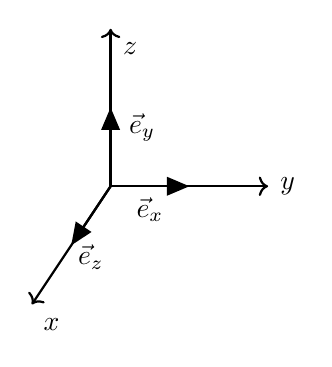
\begin{tikzpicture}
%\draw[step=0.5cm,gray,very thin] (0,0) grid (4,4); %background grid

\draw [thick,->] (1.5,2) -- (3.5,2);
\draw [thick,->] (1.5,2) -- (1.5,4);
\draw [thick,->] (1.5,2) -- (0.5,0.5);

\node[] at (0.75,0.25) {$x$};
\node[] at (3.75,2) {$y$};
\node[] at (1.75,3.75) {$z$};

\draw[>=triangle 45, line width=0.3mm, ->] (1.5,2) -- (2.5,2) ;   
\node[] at (2,1.7) {$\vec{e}_x$};

\draw[>=triangle 45, line width=0.3mm, ->] (1.5,2) -- (1.5,3) ;   
\node[] at (1.9,2.75) {$\vec{e}_y$};

\draw[>=triangle 45, line width=0.3mm, ->] (1.5,2) -- (1,1.25) ;   
\node[] at (1.25,1.1) {$\vec{e}_z$};

\end{tikzpicture}
\end{center}


\noindent Any vector can then be written
\[
{\vec V}  = V_x {\vec e}_x  + V_y {\vec e}_y + V_z \vec{e}_z
\]
The gradient of a function $f$ is 
\[
\vec{\nabla} f= \text{grad }f= 
\frac{\partial f}{\partial x}\; \vec{e}_x +
\frac{\partial f}{\partial y}\; \vec{e}_y +
\frac{\partial f}{\partial z}\; \vec{e}_z,
\]
the divergence of a vector $\vec{V}$ is
\[
\vec{\nabla}\cdot \vec{V} = 
\frac{\partial V_x}{\partial x}+
\frac{\partial V_y}{\partial y}+
\frac{\partial V_z}{\partial z}
\]
and the Laplace operator of a function $f$ is:
\[
\Delta f = 
\frac{\partial^2 f}{\partial x^2} + 
\frac{\partial^2 f}{\partial y^2} + 
\frac{\partial^2 f}{\partial z^2}  
\]
Finally the path increment is
\[
d\vec{r} = dx \; {\vec e}_x  + dy\; {\vec e}_y + dz \; \vec{e}_z
\]
and the volume element is 
\[
dV=dx\; dy \; dz
\]

%........................................
\subsubsection{Polar coordinates}

We have $r>0$ and $\theta=[0,2\pi[$, defined in the $(x,y)-$plane.

\begin{flushright} {\tiny {\color{gray} (tikz\_polar\_coordinates.tex)}} \end{flushright}
%~~~~~~~~~~~~~~~~~~~~~~~~~~~~~~~~~~~~~~~~~~~~~~~~~~~~~~~~~~~~~~~~~~~~~~~~~~~~~~~~~~~~~~~~~~~~~~~~~~
\begin{center}
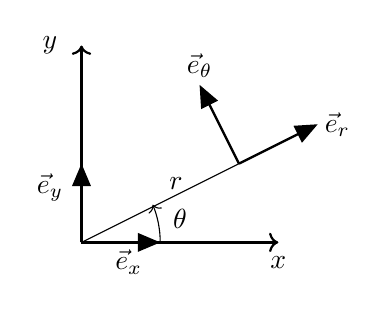
\begin{tikzpicture}
%\draw[step=0.5cm,gray,very thin] (0,0) grid (4.5,4); %background grid

\draw [thick,->] (1,1) -- (3.5,1);
\draw [thick,->] (1,1) -- (1,3.5);

\node[] at (3.5,0.75) {$x$};
\node[] at (0.6,3.5) {$y$};

\draw[>=triangle 45, line width=0.3mm, ->] (1,1) -- (2,1) ;   
\node[] at (1.6,0.75) {$\vec{e}_x$};

\draw[>=triangle 45, line width=0.3mm, ->] (1,1) -- (1,2) ;   
\node[] at (0.6,1.7) {$\vec{e}_y$};

\draw [-] (1,1) -- (3,2);

\draw[>=triangle 45, line width=0.3mm, ->] (3,2) -- (4,2.5) ;   
\node[] at (4.25,2.5) {$\vec{e}_r$};

\draw[>=triangle 45, line width=0.3mm, ->] (3,2) -- (2.5,3) ;   
\node[] at (2.5,3.25) {$\vec{e}_\theta$};


\node[] at (2.2,1.75) {$r$};
\node[] at (2.25,1.3) {$\theta$};

\draw[->] (2,1) arc (0:22.5:1.25);

\end{tikzpicture}
\end{center}


\noindent The relation between the unit vector in Cartesian and Polar/Cylindrical coordinates
is given by:
\[
\left(
\begin{array}{c}
{\vec e}_{r} \\
{\vec e}_{\theta} \\
\end{array}
\right)
=
\left(
\begin{array}{cc}
\cos \theta & \sin \theta \\
-\sin \theta & \cos \theta
\end{array}
\right)
\cdot
\left(
\begin{array}{c}
{\vec e}_{x} \\
{\vec e}_{y} \\
\end{array}
\right)
\]
which should be read:
\begin{eqnarray}
{\vec e}_{r}      &=& \cos\theta \; {\vec e}_{x} + \sin\theta \;  {\vec e}_{y} \nn\\
{\vec e}_{\theta} &=& -\sin\theta \; {\vec e}_{x} + \cos\theta \;  {\vec e}_{y} 
\end{eqnarray}
Note that this $2\times 2$ matrix is a 
rotation matrix\footnote{\url{https://en.wikipedia.org/wiki/Rotation_matrix}}
corresponding to an angle $-\theta$. The inverse of this matrix always exists 
(we can always counter-rotate) and it then yields
\[
\left(
\begin{array}{c}
{\vec e}_{x} \\
{\vec e}_{y} \\
\end{array}
\right)
=
\left(
\begin{array}{cc}
\cos \theta & -\sin \theta \\
\sin \theta & \cos \theta
\end{array}
\right)
\cdot
\left(
\begin{array}{c}
{\vec e}_{r} \\
{\vec e}_{\theta} \\
\end{array}
\right)
\]
so that for any vector ${\vec V}$
\begin{eqnarray}
{\vec V} 
&=& V_x {\vec e}_x  + V_y {\vec e}_y \nonumber\\
&=& V_x [(\cos \theta) {\vec e}_r - (\sin \theta) {\vec e}_\theta]  + 
    V_y [(\sin \theta) {\vec e}_r + (\cos \theta){\vec e}_\theta] \nonumber\\
&=& [V_x (\cos \theta) + V_y (\sin \theta)] {\vec e}_r +
[- V_x(\sin \theta) + V_y (\cos \theta)]{\vec e}_\theta \nn\\
&=& V_r \vec{e}_r  + V_\theta \vec{e}_\theta \nn
\end{eqnarray}
with
\begin{eqnarray}
V_r &=& V_x \cos \theta + V_y \sin \theta \nn\\
V_\theta &=& - V_x \sin \theta + V_y \cos \theta \nn
\end{eqnarray}
Finally the path increment is
\[
d\vec{r} = dr \; {\vec e}_r  + r \sin\theta d\theta \; {\vec e}_\theta
\]
and the volume element is 
\[
dV= r dr \; d\theta
\]

The gradient, divergence and Laplacian formulae are given in the following section.

\index{general}{Path Increment in Polar Coordinates}

%...........................................................
\subsubsection{Cylindrical coordinates \label{ss:cylcoord}}

%Redo with tikz
\begin{center}
\includegraphics[width=4cm]{images/cylindrical}\\
{\captionfont Cylindrical coordinates}
%https://tutorial.math.lamar.edu/classes/calcii/CylindricalCoords.aspx 
\end{center}

\[
{\vec V} 
= V_r \; \vec{e}_r  + V_\theta \; \vec{e}_\theta + V_z \; \vec{e}_z
\]
We have 
\begin{eqnarray}
x &=& r \; \cos\theta \nn\\
y &=& r \; \sin \theta \nn\\\ 
r &=& \sqrt{x^2+y^2} \nn
\end{eqnarray}

Let $f(r,\theta)$ be a function of the spatial coordinates. It s gradient is then
\[
\vec \nabla f
= \frac{\partial f}{\partial r} \; \vec{e}_r 
+ \frac{1}{r} \frac{\partial f}{\partial \theta} \; \vec{e}_\theta
+ \frac{\partial f}{\partial r} \; \vec{e}_z
\]
The divergence of a vector field $\vec{V}$ is 
\[
\vec\nabla \cdot \vec{V} 
= \frac{1}{r} \frac{\partial }{\partial r} (r V_r) 
+ \frac{1}{r} \frac{\partial V_\theta}{\partial \theta} 
+ \frac{\partial V_z}{\partial z}
\]
and the Laplacian of $f$ is
\[
\Delta f = \frac{1}{r} \frac{\partial }{\partial r} \left( r \frac{\partial f}{\partial r} \right)
+ \frac{1}{r^2} \frac{\partial^2 f}{\partial \theta^2} 
+ \frac{\partial^2 f}{\partial z^2} 
\]
Finally the path increment is
\[
d\vec{r} = dr \; {\vec e}_r  + r \sin\theta d\theta \; {\vec e}_\theta + dz \; \vec{e}_z
\]
and the volume element is 
\[
dV= r dr \; d\theta \; dz
\]
\index{general}{Gradient Operator in Cylindrical Coordinates}
\index{general}{Divergence Operator in Cylindrical Coordinates}
\index{general}{Laplace Operator in Cylindrical Coordinates}
\index{general}{Path Increment in Cylindrical Coordinates}

\begin{remark} 
Cylindrical coordinates can also be denoted by $(\rho,\theta)$, $(r,\phi)$ or even $(\rho,\phi)$.
They are sometimes called "cylindrical polar coordinates" or "polar cylindrical coordinates".
\end{remark}

%........................................
\subsubsection{Spherical coordinates \label{ss:sphercoord}}

On the following figure are represented the three Cartesian axis, 
a point and its spherical coordinates $r,\theta,\phi$:
\begin{center}
\includegraphics[width=5cm]{images/sphcoord}\\
{\captionfont Spherical coordinates as commonly used in physics:\\ polar angle $\theta$, and azimuthal angle $\phi$.} 
\end{center}
In this case $\theta\in[0:\pi]$ and $\phi\in]-\pi:\pi]$ and we have the following relationships:
\begin{eqnarray}
r &=& \sqrt{x^2+y^2+z^2} \\
\theta &=& \arccos (z/r) \\
\phi &=& \arctan (y/x) \\
x &=& r \sin \theta \cos \phi \\
y &=& r \sin\theta \sin\phi \\
z &=& r \cos\theta 
\end{eqnarray}
The inverse tangent used to compute $\phi$ must be suitably defined, 
taking into account the correct quadrant of $(x,y)$,
which is why the atan2 intrinsic function is used in \textsc{FORTRAN} for example.    
This is often written as follows:
\begin{eqnarray}
\theta &=& \arctan \left(\sqrt{x^2+y^2},z\right) \\
\phi &=& \arctan (y,x) 
\end{eqnarray}
where we formally take advantage of the two argument arctan
function to eliminate quadrant confusion.

The path increment is expressed as:

\begin{equation}
d\vec{r} = dr \; \vec{e}_r + r d\theta \; \vec{e}_\theta + r \sin\theta d\phi \; \vec{e}_\phi
\end{equation}
The gradient of a function $f(r,\theta,\phi)$ is 
\begin{equation}
\vec\nabla f= \frac{\partial f}{\partial r} \; \vec{e}_r
+ \frac{1}{r} \frac{\partial f}{\partial \theta} \; \vec{e}_\theta 
+ \frac{1}{r \; \sin\theta} \frac{\partial f}{\partial \phi} \;  \vec{e}_\phi
\end{equation}
The divergence of a vector $\vec{V}$ is
\begin{equation}
\vec\nabla\cdot \vec{V}=
\frac{1}{r^2} \frac{\partial}{\partial r} \left(r^2 V_r \right) 
+
\frac{1}{r \sin\theta} \frac{\partial}{\partial \theta} (V_\theta \sin\theta)
+
\frac{1}{r \sin\theta} \frac{\partial V_\phi}{\partial \phi}=0
\label{eq:divsc}
\end{equation}
The Laplacian of function $f$ is given by: \index{general}{Laplacian}
\begin{equation}
\Delta f= \vec\nabla \cdot\vec\nabla f= \vec\nabla^2 f
=
\frac{1}{r^2}\frac{\partial}{\partial r} \left( r^2 \frac{\partial f}{\partial r} \right)
+\frac{1}{r^2 \sin\theta} \frac{\partial}{\partial \theta} \left( \sin\theta \frac{\partial f}{\partial \theta} \right)
+\frac{1}{r^2 \sin^2\theta}  \frac{\partial^2 f}{\partial \phi^2}
\end{equation}

In geography one uses latitude and longitude, represented hereunder:
\begin{center}
\includegraphics[width=10cm]{images/map.jpg}
\end{center}
\begin{itemize}
\item Latitude  $\in[-90:90]$,   or $\in[-\pi/2:\pi/2]$ 
\item Longitude $\in]-180:180]$, or $\in]-\pi:\pi]$ 
\end{itemize}

Since the colatitude is the complementary angle of the latitude, 
i.e. the difference between 90 and the latitude, 
where southern latitudes are denoted with a minus sign,
$\theta$ as shown above is actually is the colatitude.
The colatitude is shown in red on the following figure: 
\index{general}{Colatitude}
\begin{center}
\includegraphics[width=3cm]{images/colatitude}
\end{center}

The volume of a sphere of radius $R$ is easily obtained by computing 
\begin{eqnarray}
V_{sphere} 
&=& \iiint_{sphere} dV \nn\\
&=& \int_0^R r^2 dr \int_0^\pi \sin\theta d\theta \int_0^{2\pi} d\phi  \nn\\
&=& \frac{1}{3}R^3  \cdot 2 \cdot 2\pi \nn\\
&=& \frac{4}{3}\pi R^3 
\end{eqnarray}
\index{general}{Volume of a Sphere}

The volume of a spherical shell of inner radius $R_i$ and outer radius $R_o$
is equally easily obtained by computing 

\begin{eqnarray}
V_{shell}
&=& \iiint_{shell} dV \nn\\
&=& \int_{R_i}^{R_o} r^2 dr \int_0^\pi \sin\theta d\theta \int_0^{2\pi} d\phi  \nn\\
&=& \frac{1}{3}(R_o^3-R_i^3)  \cdot 2 \cdot 2\pi \nn\\
&=& \frac{4}{3}\pi (R^3_o -R^3_i)
\end{eqnarray}
\index{general}{Volume of a Spherical shell}


\noindent The spherical unit vectors are related to the Cartesian unit vectors by:
\[
\left(
\begin{array}{c}
\vec{e}_{r} \\ \vec{e}_\theta \\ \vec{e}_\phi
\end{array}
\right)
=
\left(
\begin{array}{ccc}
\sin\theta \cos\phi & \sin\theta\sin\phi & \cos\theta  \\
\cos\theta \cos\phi & \cos\theta\sin\phi & -\sin\theta \\
-\sin\phi & \cos\phi & 0
\end{array}
\right)
\left(
\begin{array}{c}
\vec{e}_{x} \\ \vec{e}_y \\ \vec{e}_z
\end{array}
\right)
\]
and the Cartesian unit vectors are related to the spherical unit vectors by

\[
\left(
\begin{array}{c}
\vec{e}_{x} \\ \vec{e}_y \\ \vec{e}_z
\end{array}
\right)
=
\left(
\begin{array}{ccc}
\sin\theta \cos\phi & \cos\theta\cos\phi & -\sin\phi  \\
\sin\theta \sin\phi & \cos\theta\sin\phi & \cos\phi \\
\cos\theta & -\sin\theta & 0
\end{array}
\right)
\left(
\begin{array}{c}
\vec{e}_{r} \\ \vec{e}_\theta \\ \vec{e}_\phi
\end{array}
\right)
\]

\begin{eqnarray}
\vec{\upnu} 
&=& u\; \vec{e}_x + v \; \vec{e}_y + w \; \vec{e}_z \\
&=& u\; ( \sin\theta \cos\phi \; \vec{e}_r +  \cos\theta\cos\phi \;  \vec{e}_{\theta} -\sin\phi \; \vec{e}_{\phi} ) \\
&+& v\; ( \sin\theta \sin\phi \; \vec{e}_r + \cos\theta\sin\phi \; \vec{e}_\theta  +  \cos\phi \;  \vec{e}_\phi  )  \\
&+& w\; ( \cos\theta \; \vec{e}_r   -\sin\theta \; \vec{e}_\theta  ) \\
&=& v_r\; \vec{e}_r + v_\theta\; \vec{e}_\theta + v_\phi\; \vec{e}_\phi 
\end{eqnarray}
with 
\begin{eqnarray}
v_r      &=&  u \sin \theta  \cos \phi  + v \sin\theta \sin \phi + w \cos\theta \\
v_\theta &=&  u \cos\theta\cos\phi + v \cos\theta\sin\phi -w \sin\theta   \\
v_\phi   &=& -u \sin\phi  + v \cos\phi  
\end{eqnarray}

%.................................................................................................
\subsubsection{Converting tensors between Cartesian and Cylindrical bases \label{ss:convcartspher}}

\[
{\bm T}_{\tiny Cyl}=
\left(
\begin{array}{ccc}
T_{rr}       & T_{r\theta}      & T_{rz} \\
T_{\theta r} & T_{\theta\theta} & T_{\theta z} \\
T_{z r}      & T_{z \theta}     & T_{zz}
\end{array}
\right)
=
\left(
\begin{array}{ccc}
 \cos \theta&\sin \theta&0 \\
-\sin \theta&\cos \theta&0 \\
0 & 0 & 1 
\end{array}
\right)
\cdot
\left(
\begin{array}{ccc}
T_{xx} & T_{xy} & T_{xz} \\
T_{yx} & T_{yy} & T_{yz} \\
T_{zx} & T_{zy} & T_{zz} 
\end{array}
\right)
\cdot
\left(
\begin{array}{ccc}
\cos \theta & -\sin \theta&0 \\
\sin \theta &  \cos \theta&0 \\
0 & 0 & 1 
\end{array}
\right)
\]

\[
{\bm T}_{\tiny Cart}=
\left(
\begin{array}{ccc}
T_{xx} & T_{xy} & T_{xz} \\
T_{yx} & T_{yy} & T_{yz} \\
T_{zx} & T_{zy} & T_{zz} 
\end{array}
\right)
=
\left(
\begin{array}{ccc}
 \cos \theta&-\sin \theta&0 \\
\sin \theta&\cos \theta&0 \\
0 & 0 & 1 
\end{array}
\right)
\cdot
\left(
\begin{array}{ccc}
T_{rr}       & T_{r\theta}      & T_{rz} \\
T_{\theta r} & T_{\theta\theta} & T_{\theta z} \\
T_{z r}      & T_{z \theta}     & T_{zz}
\end{array}
\right)
\cdot
\left(
\begin{array}{ccc}
\cos \theta & \sin \theta&0 \\
-\sin \theta &  \cos \theta&0 \\
0 & 0 & 1 
\end{array}
\right)
\]



%.................................................................................................
\subsubsection{Converting tensors between Cartesian and Spherical bases \label{ss:convcartspher}}

Let ${\bm T}$ be a tensor
\[
{\bm T}=
\left(
\begin{array}{ccc}
T_{xx} & T_{xy} & T_{xz} \\
T_{yx} & T_{yy} & T_{yz} \\
T_{zx} & T_{zy} & T_{zz} 
\end{array}
\right)
\qquad\qquad
{\bm T}=
\left(
\begin{array}{ccc}
T_{rr}       & T_{r\theta}      & T_{r\phi} \\
T_{\theta r} & T_{\theta\theta} & T_{\theta\phi} \\
T_{\phi r}   & T_{\phi \theta}  & T_{\phi\phi}
\end{array}
\right)
\]
in the Cartesian basis (left) and the spherical basis (right).

The two sets of components are related by
\[
\left(
\begin{array}{ccc}
T_{xx} & T_{xy} & T_{xz} \\
T_{yx} & T_{yy} & T_{yz} \\
T_{zx} & T_{zy} & T_{zz} 
\end{array}
\right)
=
\left(
\begin{array}{ccc}
\sin\theta \; \cos\phi & \cos\theta \; \cos\phi & -\sin\phi \\
\sin\theta \; \sin\phi & \cos\theta \; \sin\phi &  \cos\phi \\
\cos\theta & -\sin\theta & 0 
\end{array}
\right)
\cdot
\left(
\begin{array}{ccc}
T_{rr}       & T_{r\theta}      & T_{r\phi} \\
T_{\theta r} & T_{\theta\theta} & T_{\theta\phi} \\
T_{\phi r}   & T_{\phi \theta}  & T_{\phi\phi}
\end{array}
\right)
\cdot
\left(
\begin{array}{ccc}
\sin\theta\;\cos\phi & \sin\theta\;\sin\phi & \cos\theta \\
\cos\theta\;\cos\phi & \cos\theta\;\sin\phi & -\sin\theta \\
-\sin\phi & \cos\phi & 0 
\end{array}
\right)
\]
or
\[
\left(
\begin{array}{ccc}
T_{rr}       & T_{r\theta}      & T_{r\phi} \\
T_{\theta r} & T_{\theta\theta} & T_{\theta\phi} \\
T_{\phi r}   & T_{\phi \theta}  & T_{\phi\phi}
\end{array}
\right)
=
\left(
\begin{array}{ccc}
\sin\theta \; \cos\phi & \sin\theta \; \sin\phi & \cos\theta \\
\cos\theta \; \cos\phi & \cos\theta \; \sin\phi & -\sin\theta \\
-\sin\phi & \cos\phi & 0 
\end{array}
\right)
\cdot
\left(
\begin{array}{ccc}
T_{xx} & T_{xy} & T_{xz} \\
T_{yx} & T_{yy} & T_{yz} \\
T_{zx} & T_{zy} & T_{zz} 
\end{array}
\right)
\cdot
\left(
\begin{array}{ccc}
\sin\theta\;\cos\phi & \cos\theta\;\cos\phi & -\sin\phi \\
\sin\theta\;\sin\phi & \cos\theta\;\sin\phi & \cos\phi \\
\cos\theta & -\sin\theta & 0
\end{array}
\right)
\]
If we now assume that the tensor ${\bm T}$ is symmetric (e.g. stress tensor, strain rate tensor),
then there are only 6 independent terms.

 \label{ss:coordsys} %-------------------
\subsection{A continuum mechanics primer} %--------------------------------------------------------
\begin{flushright} {\tiny {\color{gray} continuum\_mechanics.tex}} \end{flushright}
%~~~~~~~~~~~~~~~~~~~~~~~~~~~~~~~~~~~~~~~~~~~~~~~~~~~~~~~~~~~~~~~~~~~~~~~~~~~~~~~~~~~~~~~~~~~~~~~~~~

{\sl Contains contributions by W. Spakman} \index{contributors}{W. Spakman}

%......................................................................
\subsubsection{Forces}

In continuum mechanics we make a distinction between two broad classes of forces:
\begin{itemize}
\item Body forces defined as force per unit volume (N/m$^3$): gravity, electro-magnetic forces
\item Tractions: Surface forces defined as force per unit surface area (N/m$^2$):
Contact forces, elastic forces per unit area, internal flow friction, pressure, ...\\
A traction is the surface average of all atomic forces exerted by
atoms on the one side on atoms on the other side of the surface.
For real-Earth processes, internal tractions are ultimately caused by
the body forces, usually gravity.


Existing mantle flow(i.e. flow that is forced elsewhere) can exert
tractions (shear stresses) on the subducting slab or for instance at
the base of lithosphere plates.
In HPT-laboratory experiments external tractions (pressure, shear
traction) are applied to a rock sample, which cause internal
tractions to balance the exerted forces.

\begin{center}
\includegraphics[width=6cm]{images/contmech/spak1}
\end{center}
\end{itemize}

%......................................................................
\subsubsection{Stress tensor and tractions}\label{sec:stresstensor}
\index{general}{Stress Tensor} 
\index{general}{Normal Stress} 
\index{general}{Shear Stress} 
\index{general}{Stress Vector} 
\index{general}{Traction}

The Cauchy tensor\footnote{\url{https://en.wikipedia.org/wiki/Cauchy_stress_tensor}} 
consists of nine components $\sigma_{ij}$  that completely define the state of stress 
at a point inside a material. 
The tensor relates a unit-length direction vector $\vec{n}$ to the so-called 'stress vector' (most commonly called 'traction') $\vec{t}(\vec{n})$ across an imaginary surface perpendicular to $\vec{n}$:
\[
\vec{t}(\vec n)= {\vec n} \cdot {\bm \sigma}
\]

\begin{center}
\includegraphics[width=7cm]{images/contmech/Components_stress_tensor_cartesian}\\
{\scriptsize Modified from original 
file on Wikipedia\footnote{\url{https://commons.wikimedia.org/wiki/File:Components_stress_tensor_cartesian.svg}}}
\end{center}

With respect to an orthonormal basis $\{\vec{e}_x,\vec{e}_y,\vec{e}_z\}$, the Cauchy stress tensor
is given by:
\begin{equation}
{\bm \sigma}=
\left(
\begin{array}{ccc}
\sigma_{xx} & \sigma_{xy} & \sigma_{xz} \\
\sigma_{yx} & \sigma_{yy} & \sigma_{yz} \\
\sigma_{zx} & \sigma_{zy} & \sigma_{zz} 
\end{array}
\right)
\end{equation}
The three diagonal elements are called normal stresses while the off-diagonal terms 
are called shear stresses.

One can easily prove (see for instance Section 3.3.6 of \cite{grbl09}) that the balance 
of angular momentum leads reduces to the statement that the Cauchy stress tensor 
is symmetric, i.e. ${\bm \sigma}={\bm \sigma}^T$.
Therefore, the stress state of the medium at any point and instant can be specified by only six independent parameters, rather than nine:
\begin{equation}
{\bm \sigma}=
\left(
\begin{array}{ccc}
\sigma_{xx} & \sigma_{xy} & \sigma_{xz} \\
\sigma_{xy} & \sigma_{yy} & \sigma_{yz} \\
\sigma_{xz} & \sigma_{yz} & \sigma_{zz} 
\end{array}
\right)
\qquad\qquad
\text{or sometimes}
\qquad\qquad
{\bm \sigma}=
\left(
\begin{array}{ccc}
\sigma_{x}  & \tau_{xy}  & \tau_{xz} \\
\tau_{xy}   & \sigma_{y} & \tau_{yz} \\
\tau_{xz}   & \tau_{yz}  & \sigma_{z} 
\end{array}
\right)
\end{equation}
where the elements $\sigma _{x}$, $\sigma _{y}$, $\sigma _{z}$ are called the orthogonal 
normal stresses (relative to the chosen coordinate system), and $\tau _{xy}$, $\tau _{xz}$,
$\tau _{yz}$ the orthogonal shear stresses.
As seen above, the SI units of both stress tensor and traction are \si{\newton\per\square\metre}.

In Cylindrical coordinates the stress tensor components are given by:
\begin{eqnarray}
\sigma_{rr} &=& -p + 2 \eta \frac{\partial \upnu_r}{\partial r}      \\
\sigma_{\theta\theta} &=& 
 -p + 2\eta \left( \frac{1}{r} \frac{\partial \upnu_\theta}{\partial\theta} +\frac{\upnu_r}{r} \right)    \\
\sigma_{zz} &=& -p + 2 \eta \frac{\partial \upnu_z}{\partial z}      \\
\sigma_{r\theta} &=& \eta \left( \frac{1}{r} \frac{\partial \upnu_r}{\partial \theta} 
+ \frac{\partial \upnu_\theta}{\partial r} - \frac{\upnu_\theta}{r} \right)  \\
\sigma_{rz} &=& \eta \left( \frac{\partial \upnu_r}{\partial z}  + \frac{\partial \upnu_z}{\partial r}\right) \\
\sigma_{\theta z} &=&  \eta \left(  \frac{1}{r} \frac{\partial \upnu_z}{\partial \theta}
+\frac{\partial \upnu_\theta}{\partial z}     \right) 
\end{eqnarray}
\index{general}{Stress Tensor (Cylindrical Coordinates)}

In Spherical coordinates the stress tensor components are given by:
\begin{eqnarray}
\sigma_{rr} &=& -p + 2 \eta \frac{\partial \upnu_r}{\partial r}      \\
\sigma_{\theta\theta} &=& 
 -p + 2\eta \left( \frac{1}{r} \frac{\partial \upnu_\theta}{\partial\theta} +\frac{\upnu_r}{r} \right)    \\
\sigma_{\phi\phi} &=& 
-p + 2\eta \left( \frac{1}{r \sin \theta} \frac{\partial \upnu_\phi}{\partial \phi} 
+\frac{\upnu_r}{r}  + \frac{\upnu_\theta \cot \theta}{r} \right) \\
\sigma_{r\theta} &=& \eta\left(  r \frac{\partial}{\partial r} \frac{\upnu_\theta}{r}  
+\frac{1}{r} \frac{\partial \upnu_r}{\partial\theta}   \right)\\
\sigma_{r\phi} &=& \eta \left( \frac{1}{r \sin\theta}\frac{\partial \upnu_r}{\partial \phi} 
+ r \frac{\partial}{\partial r} \frac{\upnu_\phi}{r}  \right)\\
\sigma_{\theta \phi} &=& \eta \left(
\frac{1}{r \sin\theta} \frac{\partial \upnu_\theta}{\partial\phi}
+\frac{\sin\theta}{r} \frac{\partial}{\partial \theta} \frac{\upnu_\phi}{\sin\theta}
\right) 
\end{eqnarray}
\index{general}{Stress Tensor (Spherical Coordinates)}

 %----------------------------------------------------------------------

\begin{center}
\begin{tabular}{lll}
\hline
Symbol & meaning & unit \\
\hline
\hline
$t$ & Time & s \\
$x,y,z$ & Cartesian coordinates & m \\
${\bm v}$ & velocity vector & m$\cdot$ s$^{-1}$\\
$\rho$ & mass density & kg/m$^3$ \\
$\eta$ & dynamic viscosity &  Pa$\cdot$ s \\
$\lambda$ & penalty parameter & Pa$\cdot$ s \\
$T$ & temperature & K \\
${\bm \nabla}$ & gradient operator & m$^{-1}$ \\
${\bm \nabla}\cdot$ & divergence operator & m$^{-1}$ \\
$p$ & pressure & Pa\\
$\dot{\bm \varepsilon}({\bm v})$ & strain rate tensor & s$^{-1}$ \\
$\alpha$ & thermal expansion coefficient & K$^{-1}$ \\
$k$ & thermal conductivity & W/(m $\cdot$ K) \\
$C_p$ & Heat capacity & J/K \\
$H$ & intrinsic specific heat production & W/kg\\
$\beta_T$ & isothermal compressibility & Pa$^{-1}$  \\
${\bm \tau}$ & deviatoric stress tensor & Pa \\
${\bm \sigma}$ & full stress tensor & Pa \\
\hline
\end{tabular}
\end{center}

%------------------------------------------------------------------------
\subsection{The heat transport equation - energy conservation equation}

Let us start from the heat transport equation as shown in Schubert, Turcotte and Olson \cite{scto01}:
\[
\rho C_p \frac{DT}{Dt} - \alpha T \frac{Dp}{Dt} = {\bm \nabla} \cdot k {\bm \nabla} T + \Phi + \rho H  
\]
with $D/Dt$ being the total derivatives so that 
\[
\frac{DT}{Dt} = \frac{\partial T}{\partial t} + {\bm v}\cdot {\bm \nabla}T
\quad\quad
\frac{Dp}{Dt} = \frac{\partial p}{\partial t} + {\bm v}\cdot {\bm \nabla}p
\]
Solving for temperature, this equation is often rewritten as follows:
\begin{mdframed}[backgroundcolor=blue!5]
\[
\rho C_p \frac{DT}{Dt} - {\bm \nabla} \cdot k {\bm \nabla} T =  \alpha T \frac{Dp}{Dt} + \Phi + \rho H  
\]
\end{mdframed}

A note on the shear heating term $\Phi$: In many publications, $\Phi$ 
is given by $\Phi=\tau_{ij}\partial_j u_i={\bm \tau}:{\bm \nabla}{\bm v}$.

\begin{eqnarray}
\Phi 
&=& \tau_{ij}\partial_j u_i \nonumber\\
&=& 2 \eta \dot{\varepsilon}_{ij}^d\partial_j u_i \nonumber\\
&=& 2 \eta \frac{1}{2}\left( \dot{\varepsilon}_{ij}^d\partial_j u_i + \dot{\varepsilon}_{ji}^d\partial_i u_j \right) \nonumber\\
&=& 2 \eta \frac{1}{2}\left( \dot{\varepsilon}_{ij}^d\partial_j u_i + \dot{\varepsilon}_{ij}^d\partial_i u_j \right) \nonumber\\
&=& 2 \eta  \dot{\varepsilon}_{ij}^d  \frac{1}{2}\left(\partial_j u_i + \partial_i u_j \right) \nonumber\\
&=& 2 \eta  \dot{\varepsilon}_{ij}^d   \dot{\varepsilon}_{ij} \nonumber\\
&=& 2 \eta  \dot{\bm \varepsilon}^d :  \dot{\bm \varepsilon} \nonumber\\
&=& 2 \eta  \dot{\bm \varepsilon}^d : \left( \dot{\bm \varepsilon}^d +\frac{1}{3} ({\bm \nabla}\cdot{\bm v}) {\bm 1} \right)\nonumber\\
&=& 2 \eta  \dot{\bm \varepsilon}^d : \dot{\bm \varepsilon}^d 
+ 2 \eta  \dot{\bm \varepsilon}^d : {\bm 1} ({\bm \nabla}\cdot{\bm v}) \nonumber\\ 
&=& 2 \eta  \dot{\bm \varepsilon}^d : \dot{\bm \varepsilon}^d 
\end{eqnarray}
Finally
\[
\Phi = {\bm \tau}:{\bm \nabla}{\bm v} = 2 \eta  \dot{\bm \varepsilon}^d : \dot{\bm \varepsilon}^d
= 2 \eta \left( (\dot{\varepsilon}_{xx}^d)^2 + (\dot{\varepsilon}_{yy}^d)^2 + 2(\dot{\varepsilon}_{xy}^d)^2 \right)
\]

%------------------------------------------------------------------------
\subsection{The momentum conservation equations} 

Because the Prandlt number is virtually zero in Earth science applications the Navier Stokes 
equations reduce to the Stokes equation:
\[
{\bm \nabla}\cdot {\bm \sigma} + \rho {\bm g} = 0
\]
Since 
\[
{\bm \sigma} = -p {\bm 1} + {\bm \tau}
\]
it also writes
\[
-{\bm \nabla}p + {\bm \nabla}\cdot {\bm \tau} + \rho {\bm g} = 0
\]
Using the relationship ${\bm \tau} = 2 \eta \dot{\bm \varepsilon}^d$ we arrive at 
\begin{mdframed}[backgroundcolor=blue!5]
\[
-{\bm \nabla}p + {\bm \nabla}\cdot (2 \eta \dot{\bm \varepsilon}^d ) + \rho {\bm g} = 0
\]
\end{mdframed}

%------------------------------------------------------------------------
\subsection{The mass conservation equations} 

The mass conservation equation is given by
\[
\frac{D\rho}{Dt} + \rho {\bm \nabla}\cdot{\bm v} = 0
\]
or, 
\begin{mdframed}[backgroundcolor=blue!5]
\[
\frac{\partial \rho}{\partial t} + {\bm \nabla}\cdot(\rho {\bm v}) = 0
\]
\end{mdframed}
In the case of an incompressible flow, then $\partial \rho/\partial t=0$ and 
${\bm \nabla}\rho=0$, i.e. $D\rho/Dt=0$ and the remaining equation is simply:
\[
{\bm \nabla}\cdot{\bm v} = 0
\]

\subsection{The equations in ASPECT manual}
The following is lifted off the ASPECT manual.
We focus on the system of equations in a $d=2$- or $d=3$-dimensional
domain $\Omega$ that describes the motion of a highly viscous fluid driven
by differences in the gravitational force due to a density that depends on
the temperature. In the following, we largely follow the exposition of this
material in Schubert, Turcotte and Olson \cite{scto01}.

Specifically, we consider the following set of equations for velocity $\mathbf
u$, pressure $p$ and temperature $T$:
\begin{align}
  \label{eq:stokes-1}
  -\nabla \cdot \left[2\eta \left(\dot\varepsilon(\bm v)
                                  - \frac{1}{3}(\nabla \cdot \bm v)\mathbf 1\right)
                \right] + \nabla p &=
  \rho \bm g
  &
  & \textrm{in $\Omega$},
  \\
  \label{eq:stokes-2}
  \nabla \cdot (\rho \bm v) &= 0
  &
  & \textrm{in $\Omega$},
  \\
  \label{eq:temperature}
  \rho C_p \left(\frac{\partial T}{\partial t} + \bm v\cdot\nabla T\right)
  - \nabla\cdot k\nabla T
  &=
  \rho H
  \notag
  \\
  &\quad
  +
  2\eta
  \left(\dot\varepsilon(\bm v) - \frac{1}{3}(\nabla \cdot \bm v)\mathbf 1\right)
  :
  \left(\dot\varepsilon(\bm v) - \frac{1}{3}(\nabla \cdot \bm v)\mathbf 1\right)
  \\
  &\quad
  +\alpha T \left( \bm v \cdot \nabla p \right)
  \notag
  \\
  &\quad
  &
  & \textrm{in $\Omega$},
  \notag
\end{align}
where $\dot{\bm \varepsilon}(\mathbf u) = \frac{1}{2}(\nabla \mathbf u + \nabla\mathbf
u^T)$ is the symmetric gradient of the velocity (often called the
\textit{strain rate}).%

In this set of equations, \eqref{eq:stokes-1} and \eqref{eq:stokes-2}
represent the compressible Stokes equations in which $\mathbf v=\mathbf
v(\mathbf x,t)$ is the velocity field and $p=p(\mathbf x,t)$ the pressure
field. Both fields depend on space $\mathbf x$ and time $t$. Fluid flow is
driven by the gravity force that acts on the fluid and that is proportional to
both the density of the fluid and the strength of the gravitational pull.

Coupled to this Stokes system is equation \eqref{eq:temperature} for the
temperature field $T=T(\mathbf x,t)$ that contains heat conduction terms as
well as advection with the flow velocity $\mathbf v$. The right hand side
terms of this equation correspond to
\begin{itemize}
\item internal heat production for example due to radioactive decay;
\item friction (shear) heating;
\item adiabatic compression of material;
\end{itemize}

In order to arrive at the set of equations that ASPECT solves, 
we need to 
\begin{itemize}
\item neglect the $\partial p/\partial t$. {\color{red}WHY?}
\item neglect the $\partial \rho / \partial t$ . {\color{red}WHY?}
\end{itemize}
from equations above. 

----------------------------------------

Also, their definition of the shear heating term $\Phi$ is:
\[
\Phi = k_B ({\bm \nabla}\cdot{\bm v})^2 + 2\eta \dot{\bm \varepsilon}^d:\dot{\bm \varepsilon}^d
\]
For many fluids the bulk viscosity $k_B$ is very small and is often taken to be zero, an assumption known
as the Stokes assumption: $k_B=\lambda+2\eta/3=0$. \index{bulk viscosity}
Note that $\eta$ is the dynamic viscosity and $\lambda$ the second viscosity. \index{dynamic viscosity}
\index{second viscosity}
Also, 
\[
{\bm \tau}=2\eta \dot{\bm \varepsilon} + \lambda ({\bm \nabla}\cdot{\bm v}) {\bm 1}
\]
but since $k_B=\lambda+2\eta/3=0$, then $\lambda=-2\eta/3$ so 
\[
{\bm \tau}=2\eta \dot{\bm \varepsilon} -\frac{2}{3}\eta ({\bm \nabla}\cdot{\bm v}) {\bm 1} = 2\eta \dot{\bm \varepsilon}^d
\]







\newpage
%---------------------------------
\subsection{the Boussinesq approximation: an Incompressible flow}

\index{Boussinesq}

[from aspect manual]
The Boussinesq approximation assumes that the density can be
considered constant in all occurrences in the equations with the exception of
the buoyancy term on the right hand side of \eqref{eq:stokes-1}. The primary
result of this assumption is that the continuity equation \eqref{eq:stokes-2}
will now read
\[
{\bm \nabla}\cdot{\bm v} = 0
\]
This implies that the strain rate tensor is deviatoric.
Under the Boussinesq approximation, the equations are much simplified:

\begin{align}
  \label{eq:stokes-1}
  -\nabla \cdot \left[2\eta \dot{\bm \varepsilon}(\bm v)
                \right] + \nabla p &=
  \rho \bm g
  &
  & \textrm{in $\Omega$},
  \\
  \label{eq:stokes-2}
  \nabla \cdot (\rho \bm v) &= 0
  &
  & \textrm{in $\Omega$},
  \\
  \label{eq:temperature}
  \rho_0 C_p \left(\frac{\partial T}{\partial t} + \bm v\cdot\nabla T\right)
  - \nabla\cdot k\nabla T
  &=
  \rho H
  &
  & \textrm{in $\Omega$}
\end{align}
Note that all terms on the rhs of the temperature equations have disappeared, with the exception 
of the source term.


\newpage
\subsection{Stokes equation for elastic medium}

What follows is mostly borrowed from Becker \& Kaus lecture notes.

%\begin{tabular}{|l|l|l|}
%\hline
%${\bm u}       $ & displacement vector &   \\
%${\bm \sigma}  $ & full stress tensor  & Pa\\
%${\bm \epsilon}$ & strain tensor       &   \\
%${\bm 1}       $ & unit tensor         &   \\
%${\bm f}       $ & body forces         &   \\
%\hline
%\end{tabular}

The strong form of the PDE that governs force balance in a medium is given by
\[
{\bm \nabla}\cdot{\bm \sigma}  + {\bm f} = {\bm 0}
\]
where ${\bm \sigma}$ is the stress tensor and ${\bm f}$ is a body force.

The stress tensor is related to the strain tensor through the generalised 
Hooke's law:
\begin{equation}
\sigma_{ij}=\sum_{kl}C_{ijkl}\epsilon{kl} \label{eq:one}
\end{equation}
where ${\bm C}$ is the fourth-order elastic tensor.
In the case of an isotropic material, this relationship simplifies to
\begin{equation}
\sigma_{ij}=\lambda \epsilon_{kk} \delta_{ij} + 2\mu \epsilon_{ij}
\quad\quad
or, 
\quad\quad
{\bm \sigma} = \lambda ({\bm \nabla}\cdot{\bm u})  {\bm 1} + 2\mu {\bm \epsilon}   \label{eq:two}
\end{equation}
where $\lambda$ is the Lam\'e parameter and $\mu$ is the shear modulus\footnote{It is also sometimes written $G$}.
The term ${\bm \nabla}\cdot{\bm u}$ is the isotropic dilation.

\index{Lam\'e parameter} \index{shear modulus}

The strain tensor is related to the displacement as follows: \index{strain tensor}
\[
{\bm \epsilon} = \frac{1}{2}({\bm \nabla}{\bm u} + {\bm \nabla}{\bm u}^T)
\]

The incompressibility (bulk modulus), $K$, is defined as $p=-K {\bm \nabla}\cdot{\bm u}$ 
where $p$ is the pressure with \index{bulk modulus}
\begin{eqnarray}
p&=&-\frac{1}{3}Tr({\bm \sigma}) \nonumber\\
 &=& -\frac{1}{3} [ \lambda ({\bm \nabla}\cdot{\bm u}) Tr[{\bm 1}] + 2 \mu Tr[{\bm \epsilon}]] \nonumber\\
 &=& -\frac{1}{3} [ \lambda ({\bm \nabla}\cdot{\bm u})  3  + 2 \mu  ({\bm \nabla}\cdot{\bm u}) ] \nonumber\\
 &=& -[ \lambda  + \frac{2}{3} \mu ]   ({\bm \nabla}\cdot{\bm u})  
\end{eqnarray}
so that $K=\lambda+\frac{2}{3}\mu$.

%or
%\[
%\mu=\frac{3K(1-2\nu)}{2(1+\nu)}
%\]


\paragraph{Remark}: Eq. (\ref{eq:one}) and (\ref{eq:two}) are analogous to the ones that one has to solve
in the context of viscous flow using the penalty method. In this case $\lambda$ is the penalty coefficient, 
${\bm u}$ is the velocity, and $\mu$ is then the dynamic viscosity.

%\begin{center}
%\includegraphics[width=15cm]{images/coeffs}\\
%{\small Homogeneous isotropic linear elastic materials have their elastic properties uniquely determined by any two moduli among these; thus, given any two, any other of the elastic moduli can be calculated according to these formulas.}
%\end{center}

The Lam\'e parameter and the shear modulus are also linked to $\nu$ the poisson ratio, 
and $E$, Young's modulus: \index{Poisson ratio} \index{Young's modulus}
\[
\lambda=\mu\frac{2\nu}{1-2\nu}
=\frac{\nu E}{(1+\nu)(1-2\nu)}
\quad\quad
{\rm with}
\quad\quad
E=2\mu(1+\nu)
\]
The shear modulus, expressed often in GPa, describes the material's response to shear stress.
The poisson ratio describes the response in the direction orthogonal to uniaxial stress.
The Young modulus, expressed in GPa, describes the material's strain response to uniaxial stress in the 
direction of this stress.









 %----------------------------------------------------------------------------------
\subsection{Rheology in geodynamics} 
For now what follows only deals with viscous behavior.


\subsubsection{Linear viscous aka Newtonian} \index{Newtonian fluid}

Simply put, a Newtonian fluid is a fluid in which the viscous stresses at every point are linearly proportional 
to the local strain rate.
Mathematically speaking, this means that the fourth-order tensor ${\bm C}$ relating the viscous stress 
tensor to the strain rate tensor does not depend on the stress state and velocity of the flow.
\[
{\bm s}={\bm C} \cdot \dot{\bm \varepsilon}
\]

One very often make sthe assumption that the fluid is isotropic, i.e. its mechanical properties are the 
same along any direction. As a consequence the fourth order viscosity tensor 
${\bm C}$ is symmetric and will have only two independent real parameters: 
a bulk viscosity coefficient, that defines the resistance of the medium to gradual uniform compression; 
and a dynamic viscosity coefficient $\eta$ that expresses its resistance to gradual shearing, 
(we here neglect the so-called rotational viscosity coefficient which results from a coupling between the fluid flow and the rotation of the individual particles). %wiki



Rather logically we denote by non-Newtonian fluids with are not Newtonian, i.e. their viscosity (tensor)
depends on stress. Such fluids are part of our daily life, e.g. honey, toothpaste, paint, blood, and shampoo. 
 


%------------------------------
\subsubsection{Power-law model}
\index{Power-law model}

One of the simplest non-Newtonian viscosity model is the power-law model:
\begin{equation}
\eta = K \dot{\varepsilon}_{II}^{(n-1)/2}
\end{equation}
where $\dot{\varepsilon}_{II}$ is the second invariant of the strain rate tensor as defined in 
Section~\ref{sec:invariants}, and $n$ and $K$ are parameters. $n$ is called the power-law index.

Note that a Newtonian viscosity is recovered when $n=1$. Also $n$ and $K$ may depend on temperature
\cite[p339]{reddybook2}.


%------------------------------
\subsubsection{Carreau model}



%------------------------------
\subsubsection{Bingham model}


%------------------------------
\subsubsection{Herschel-Bulkley visco-plastic model}

The Herschel-Bulkley model is effectively a combination of the power-law model and 
a simple plastic model:
\begin{eqnarray}
{\bm s} &=& 2 \left(  K \dot{\varepsilon}^{n-1} + \frac{\tau_0}{\dot{\varepsilon}}\right)\dot{\bm \varepsilon} \qquad \text{ if } {s}_{II}>\tau_0 \\
\dot{\bm \varepsilon} &=& {\bm 0} \qquad {s}_{II} \leq \tau_0 \\
\end{eqnarray}
in which $\dot{\varepsilon}=\sqrt{\dot{\varepsilon}_{II}}$, 
$\tau_0$ is the yield stress, $K$ the consistency, and $n$ is the flow index \cite{bemj04}.
The flow index measures the degree to which the fluid is shear-thinning ($n<1$) or shear-thickening ($n>1$).
If $n=1$ and $\tau_0=0$ the model reduces to the Newtonian model. 

The term between parenthesis above is the nonlinear effective viscosity. Concretely, the implementation goes as 
follows\footnote{\url{https://en.wikipedia.org/wiki/Herschel-Bulkley_fluid}}:
\[
\eta_{eff} = 
\left\{
\begin{array}{cc}
\eta_0 & \dot{\varepsilon}\leq \dot{\varepsilon}_0 \\ 
K \dot{\varepsilon}^{n-1} + \frac{\tau_0}{\dot{\varepsilon}} & \dot{\varepsilon} \geq \dot{\varepsilon}_0
\end{array}
\right.
\]
The limiting viscosity $\eta_0$ is chosen such that 
$\eta_0 =  K \dot{\varepsilon}_0^{n-1} + \frac{\tau_0}{\dot{\varepsilon}_0}$

A large limiting viscosity means that the fluid will only flow in response to a large applied force. 
This feature captures the Bingham-type behaviour of the fluid. 
Note that when strain rates are large, the power-law behavior dominates. 

As we have seen for Bingham fluids, the equations above are not easily amenable to implementation so that 
one usually resorts to regularisation, which is a modification of the 
equations by introducing a new material parameter which controls the exponential 
growth of stress. This way the equation is valid for both yielded and unyielded areas
\cite{blmi97,papa87}:
\[
\eta_{eff} = K \dot{\varepsilon}^{n-1} + \frac{\tau_0}{\dot{\varepsilon}} [1 - \exp(-m \dot{\varepsilon})] 
\]
When the strain rate becomes (very) small a Taylor expansion of the regularisation 
term yields $1- \exp(-m \dot{\varepsilon}) \sim m \dot{\varepsilon} $ so that 
$\eta_{eff} \rightarrow m \tau_0$.

\todo[inline]{Channel flow of wikipedia with analytical solution!}


%------------------------------
\subsubsection{Dislocation creep}

%------------------------------
\subsubsection{Diffusion creep}

%------------------------------
\subsubsection{Peierls creep}



 %--------------------------------------------
\subsection{Moment of inertia} \begin{flushright} {\tiny {\color{gray} momentofinertia.tex}} \end{flushright}

% borrowed from http://farside.ph.utexas.edu/teaching/336k/Newtonhtml/node64.html

Consider a rigid body rotating with fixed angular velocity $\omega$ about an axis which passes through the origin.
Let ${\bm r}_i$ be the position vector of the $i$th mass element, whose 
mass is $m_i$. We expect this position vector to precess about the axis of rotation (which is parallel to $\omega$) 
with angular velocity $\omega$. 

\begin{displaymath} 
\frac{d{\bm r}_i}{dt} = \mbox{\boldmath$\omega$}\times {\bm r}_i. 
\end{displaymath}

Thus, the above equation specifies the velocity, ${\bm v}_i = d{\bm r}_i/dt$, of each mass element as the body rotates with fixed angular velocity $\omega$ about an axis passing through the origin. 


The total angular momentum of the body (about the origin) is written
\begin{displaymath} 
{\bm L} 
= \sum_{i=1,N} m_i\,{\bm r}_i\times\frac{d{\bm r}_i}{dt}
= \sum_{i=1,N} m_i\,{\bm r}_i\times ( \mbox{\boldmath$\omega$}\times {\bm r}_i )
= \sum_{i=1,N} m_i\, [ r_i^2 {\bm \omega} - ({\bm r}_i\cdot {\bm \omega}) {\bm r}_i ]
\end{displaymath}
The above formula can be written as a matrix equation of the form
\begin{displaymath} 
\left(\begin{array}{c}L_x\\ L_y\\ L_z\end{array}\right)=
\left(\begin{array}{ccc}
I_{xx} & I_{xy} & I_{xz} \\
I_{yx} & I_{yy} & I_{yz} \\
I_{zx} & I_{zy} & I_{zz} 
\end{array}\right) 
\left(\begin{array}{c}\omega_x\\ \omega_y\\ \omega_z\end{array}\right)
\end{displaymath}
where

\begin{eqnarray}
I_{xx}       &=& + \sum_{i=1,N}(y_i^{\,2}+z_i^{\,2}) \,m_i= \int(y^2+ z^2)\,dm = \int_V (y^2+ z^2)\,\rho(x,y,z) dV   \nonumber\\
I_{yy}       &=& + \sum_{i=1,N}(x_i^{\,2}+z_i^{\,2}) \,m_i= \int(x^2+ z^2)\,dm = \int_V (x^2+ z^2)\,\rho(x,y,z) dV   \nonumber\\
I_{zz}       &=& + \sum_{i=1,N}(x_i^{\,2}+y_i^{\,2}) \,m_i= \int(x^2+ y^2)\,dm = \int_V (x^2+ y^2)\,\rho(x,y,z) dV   \nonumber\\
I_{xy}=I_{yx}&=& - \sum_{i=1,N}x_i\,y_i \,m_i=- \int x\,y\,dm =- \int x\,y\,\rho(x,y,z) dV   \nonumber\\
I_{yz}=I_{zy}&=& - \sum_{i=1,N}y_i\,z_i \,m_i= -\int y\,z\,dm =- \int y\,z\,\rho(x,y,z) dV   \nonumber\\
I_{xz}=I_{zx}&=& - \sum_{i=1,N}x_i\,z_i \,m_i= -\int x\,z\,dm =- \int x\,z\,\rho(x,y,z) dV   \nonumber
\end{eqnarray}

Here, $I_{xx}$ is called the moment of inertia about the $x$-axis, $I_{yy}$ the moment of inertia about the $y$-axis, $I_{xy}$ the $xy$ product of inertia, $I_{yz}$ the $yz$ product of inertia, etc.
The matrix of the $I_{ij}$ values is known as the moment of inertia tensor.

 In general, the angular momentum vector, ${\bf L}$ points in a different direction to the angular velocity vector, $\omega$. In other words, ${\bf L}$ is generally not parallel to $\omega$.

Finally, although the above results were obtained assuming a fixed angular velocity, 
they remain valid at each instant in time if the angular velocity varies.

In the simplified case of a spherically symmetric planet, it is easy to see that $I_{xx}=I_{yy}=I_{zz}$ so that $I=\frac{1}{3}(I_{xx}+I_{yy}+I_{zz})$, and $\rho=\rho(r)$ with $dV=4\pi r^2 dr$, leading to
\[
I=\frac{8\pi}{3}\int_0^R \rho(r) r^4 dr
\]
Assuming further that the planet has a constant density $\rho_0$, we obtain 
\[
I=\frac{8 \pi}{3} \rho_0 \int_0^R  r^4 dr = \frac{8 \pi}{3} \rho_0 \frac{R^5}{5} = \frac{2}{5} M R^2 
\]
where $M$ is the mass of the planet and $R$ is its radius.

Assuming now that the planet is composed of a core of radius $R_c$ and density $\rho_c$ surrounded by a mantle of density $\rho_m$, 
we have
\[
I=\frac{8\pi}{3}\int_0^R \rho(r) r^4 dr
=\frac{8\pi}{3} \left( \int_0^{R_c} \rho_c r^4 dr +  \int_{R_c}^{R} \rho_m r^4 dr \right)
=\frac{8\pi}{15} \left( \rho_c R_c^5  +  \rho_m (R^5-R_c^5) \right)
\] 

The moment of inertia of the core is given in Table 2 of "Core Dynamics", Treatise on Geophysics, edited by Peter Olson:
$I_{core}=9.2\times10^{36} kg.m^2$. The total moment of inertia for the Earth is then given by $I=I_{core}+I_{mantle}$.



\subsection{The need for numerical modelling}

The governing equations we have seen in this chapter require the use 
of numerical solution techniques for three main reasons:
\begin{itemize}
\item the advection term in the energy equation couples velocity and temperature;
\item the constitutive law (the relationship between stress and strain rate) 
often depends on velocity (or rather, strain rate), temperature, pressure, ...
\item Even when the coefficients of the PDE's are linear, often their spatial
variability, coupled to potentially complex domain geometries prevent 
arriving at the analytical solution.
\end{itemize}

Also we often have to deal with additional challenges:
\begin{itemize}
\item Complex geometries
\item Multiphysics 
\item Many scales in space and time
\end{itemize}


Note that in CFD one makes a distinction between verification and validation. 
Simply put \cite{roac97}:
\begin{itemize}
\item verification: "solving the equations right"
\item validation: "solving the right equations"
\end{itemize}
\index{general}{Verification}
\index{general}{Validation}



 %%%%%%%%%%%%%%%%%%%%%%%%%%%%%%%%%%%%%%%%%%%%%%%%%%%%%%%%%%%%%%%%%%%%%%%%%%%%%%%%

%%%%%%%%%%%%%%%%%%%%%%%%%%%%%%%%%%%%%%%%%%%%%%%%%%%%%%%%%%%%%%%%%%%%%%%%%%%%%%%%%%%%%%%%%%%%%%%%%%%
%\chapter{The building blocks of the Finite Element Method} %%%%%%%%%%%%%%%%%%%%%%%%%%%%%%%%%%%%%%%

\subsection{Numerical integration} \label{sec:quadrature}As we will see later, using the Finite Element method to solve problems involves computing integrals which are more often than not too complex to be computed analytically/exactly. We will then need to compute them numerically.

[wiki] In essence, 
the basic problem in numerical integration is to compute an approximate solution to a definite integral
\[
\int_a^b f(x) dx
\]
to a given degree of accuracy.
This problem has been widely studied and we know that 
if $f(x)$ is a smooth function, and the domain of integration is bounded, there are many methods for approximating the integral to the desired precision.

There are several reasons for carrying out numerical integration.
\begin{itemize}
\item The integrand $f(x)$ may be known only at certain points, such as obtained by sampling. Some embedded systems and other computer applications may need numerical integration for this reason.
\item A formula for the integrand may be known, but it may be difficult or impossible to find an antiderivative that is an elementary function. An example of such an integrand is $f(x)=exp(-x^2)$, the antiderivative of which (the error function, times a constant) cannot be written in elementary form.
\item It may be possible to find an antiderivative symbolically, but it may be easier to compute a numerical approximation than to compute the antiderivative. That may be the case if the antiderivative is given as an infinite series or product, or if its evaluation requires a special function that is not available.
\end{itemize}

%-----------------------------
\subsubsection{in 1D - theory}

The simplest method of this type is to let the interpolating function be a constant function (a polynomial of degree zero) that passes through the point $((a+b)/2, f((a+b)/2))$.

This is called the midpoint rule \index{midpoint rule} or rectangle rule. \index{rectangle rule}
\[
\int_a^b f(x)dx \simeq (b-a) f(\frac{a+b}{2})
\]

\improvement[inline]{insert here figure}

The interpolating function may be a straight line (an affine function, i.e. a polynomial of degree 1)
passing through the points $(a, f(a))$ and $(b, f(b))$.

This is called the trapezoidal rule. \index{trapezoidal rule} 
\[
\int_a^b f(x)dx \simeq (b-a) \frac{f(a)+f(b)}{2}
\]

\improvement[inline]{insert here figure}

For either one of these rules, we can make a more accurate approximation by breaking up the interval [a, b] into some number n of subintervals, computing an approximation for each subinterval, then adding up all the results. This is called a composite rule, extended rule, or iterated rule. For example, the composite trapezoidal rule can be stated as

\[
\int_a^b f(x)dx \simeq \frac{b-a}{n} \left( \frac{f(a)}{2}  
+\sum_{k=1}^{n-1} f(a+k\frac{b-a}{n})
   +\frac{f(b)}{2} \right)
\]

where the subintervals have the form $[kh,(k+1)h]$, with $h=(b-a)/n$ and $k=0,1,2,\dots,n-1$.


\begin{center}
a)\includegraphics[width=7cm]{images/quadrature/int1}
b)\includegraphics[width=7cm]{images/quadrature/int2}\\
The interval $[-2,2]$ is broken into 16 sub-intervals. The blue lines correspond to the 
approximation of the red curve by means of a) the midpoint rule,  b) the trapezoidal rule.
\end{center}

There are several algorithms for numerical integration (also commonly called 'numerical quadrature', or
simply 'quadrature') \index{quadrature}.
Interpolation with polynomials evaluated at equally spaced points in $[a,b]$
yields the Newton–Cotes formulas, of which the rectangle rule and the trapezoidal rule are examples. \index{Newton-Cotes}
If we allow the intervals between interpolation points to vary, we find another group of quadrature formulas, such as 
the Gauss(ian) quadrature formulas. \index{Gauss quadrature}
A Gaussian quadrature rule is typically more accurate than a Newton–Cotes rule, 
which requires the same number of function evaluations, if the integrand is smooth 
(i.e., if it is sufficiently differentiable).


An $n-$point Gaussian quadrature rule, named after Carl Friedrich Gauss, is a quadrature rule constructed
to yield an exact result for polynomials of degree $2n-1$ or less by a suitable choice of the points $x_i$
and weights $w_i$ for $i=1,\dots,n$.

The domain of integration for such a rule is conventionally taken as $[-1,1]$, so the rule is stated as
\[
\int_{-1}^{+1} f(x) dx = \sum_{i_q=1}^n w_{i_q} f(x_{i_q})
\]
In this formula the $x_{i_q}$ coordinate is 
the $i$-th root of the Legendre polynomial $P_n(x)$. \index{Legendre polynomial}

It is important to note that a Gaussian quadrature will only produce good results if the function $f(x)$
is well approximated by a polynomial function within the range $[-1,1]$.
As a consequence, the method is not, for example, suitable for functions with singularities.

\begin{center}
\includegraphics[width=5.cm]{images/quadrature/gq2}\\
Gauss-Legendre points and their weights.
\end{center}

As shown in the above table, it can be shown that the weight values must fulfill the following condition:
\begin{equation}
\sum_{i_q} w_{i_q}=2 \label{gq23}
\end{equation}
and it is worth noting that all quadrature point coordinates are symmetrical around the origin.

Since most quadrature formula are only valid on a specific interval, we now must address the problem 
of their use outside of such intervals. The solution turns out to be quite simple: one 
must carry out a change of variables from the interval $[a,b]$ to $[-1,1]$.

We then consider the reduced coordinate $r\in[-1,1]$ such that 
\[
r=\frac{2}{b-a}(x-a)-1 
\]
This relationship can be reversed such that when $r$ is known, its equivalent coordinate 
$x\in[a,b]$ can be computed:
\[
x=\frac{b-a}{2}(1+r)+a
\]
From this it follows that
\[
dx=\frac{b-a}{2}dr
\]
and then 
\[
\int_a^b f(x) dx  = \frac{b-a}{2} \int_{-1}^{+1} f(r) dr \simeq 
\frac{b-a}{2} \sum_{i_q=1}^n w_{i_q} f(r_{i_q})
\]

%--------------------
\subsubsection{in 1D - examples}

\paragraph{example 1}

Since we know how to carry out any required change of variables, we choose for simplicity 
$a=-1$, $b=+1$.
Let us take for example $f(x)=\pi$. Then we can compute the integral of this function 
over the interval $[a,b]$ exactly:
\[
I=\int_{-1}^{+1} f(x) dx = \pi \int_{-1}^{+1}dx  = 2 \pi
\]
We can now use a Gauss-Legendre formula to compute this same integral:
\[
I_{gq}=\int_{-1}^{+1} f(x) dx 
= \sum_{i_q=1}^{n_q} w_{i_q} f(x_{i_q}) 
= \sum_{i_q=1}^{n_q} w_{i_q} \pi
= \pi \underbrace{\sum_{i_q=1}^{n_q} w_{i_q} }_{=2}
= 2 \pi
\]
where we have used the property of the weight values of Eq.(\ref{gq23}).
Since the actual number of points was never specified, this result is valid for all 
quadrature rules.


\paragraph{example 2}

Let us now take $f(x)=m x+ p$ and repeat the same exercise:
\[
I=\int_{-1}^{+1} f(x) dx = \int_{-1}^{+1} (mx+p) dx  =  [\frac{1}{2} m x^2 + p x ]_{-1}^{+1} =2p
\]
\[
I_{gq}=\int_{-1}^{+1} f(x) dx 
\!= \sum_{i_q=1}^{n_q} w_{i_q} f(x_{i_q}) 
\!= \sum_{i_q=1}^{n_q} w_{i_q} (m x_{i_q} + p)  
\!= m \underbrace{\sum_{i_q=1}^{n_q} w_{i_q} x_{i_q}}_{=0}  + p \underbrace{\sum_{i_q=1}^{n_q} w_{i_q}}_{=2}  = 2p
\]
since the quadrature points are symmetric w.r.t. to zero on the x-axis.
Once again the quadrature is able to compute the exact value of this integral: this makes sense since 
an $n$-point rule exactly integrates a $2n-1$ order polynomial such that a 1 point quadrature exactly 
integrates a first order polynomial like the one above.



\paragraph{example 3}

Let us now take $f(x)=x^2$. We have 
\[
I=\int_{-1}^{+1} f(x) dx = \int_{-1}^{+1} x^2 dx  =  [\frac{1}{3}x^3 ]_{-1}^{+1} =  \frac{2}{3} 
\]
and 
\[
I_{gq}=\int_{-1}^{+1} f(x) dx 
\!= \sum_{i_q=1}^{n_q} w_{i_q} f(x_{i_q}) 
\!= \sum_{i_q=1}^{n_q} w_{i_q} x_{i_q}^2 
\]

\begin{itemize}
\item $n_q=1$: $x_{iq}^{(1)}=0$, $w_{i_q}=2$. $I_{gq}=0$
\item $n_q=2$: $x_{q}^{(1)}=-1/\sqrt{3}$, $x_{q}^{(2)}=1/\sqrt{3}$, $w_{q}^{(1)}=w_{q}^{(2)}=1$. $I_{gq}=\frac{2}{3}$
\item It also works $\forall n_q>2$ !
\end{itemize}

%-----------------------------
\subsubsection{in 2D/3D - theory}


Let us now turn to a two-dimensional integral of the form
\[
I=\int_{-1}^{+1} \int_{-1}^{+1} f(x,y) dx dy
\]
The equivalent Gaussian quadrature writes:
\[
I_{gq}
\simeq \sum_{i_q=1}^{n_q}\sum_{j_q}^{n_q} f(x_{i_q},y_{j_q}) w_{i_q} w_{j_q}
\]


%----------------------------------------
\subsubsection{quadrature on tetrahedra}

Quadrature rules on tetrahedra take the form:
\[
\int\int\int_{el} f(x,y,z) dxdydz = V_{el} \sum_{iq=1}^{nqel} w_{iq} f(\xi^{iq}_1,\xi^{iq}_2,\xi^{iq}_3,\xi^{iq}_4) 
\]
or, that is to say:
\[
\int\int\int_{el} f(x,y,z) dxdydz = \sum_{iq=1}^{nqel} (w_{iq}V_{el}) f(\xi^{iq}_1,\xi^{iq}_2,\xi^{iq}_3,\xi^{iq}_4) 
\]
with in our case $V_{el}=1/6$.

In the literature it can be found that a one point quadrature is characterised by 
\[
w_{iq}=1 \quad\quad\quad \xi^{iq}_1=\xi^{iq}_2=\xi^{iq}_3=\xi^{iq}_4=0.25
\]
i.e, the coordinates of the single point are given by:
\[
x_{iq}=\sum_{i=1}^4 \xi_i^{iq} x_i = \frac{1}{4} (x_1+x_2+x_3+x_4)
\]
Same for $y$ and $z$ coordinates. 

A four-point quadrature rule is characterised by $w_{iq}=0.25$ and 

\begin{tabular}{lcccc}
 & $\xi_1$ & $\xi_2$ & $\xi_3$ & $\xi_4$ \\
iq=1 & 0.585410196624969 & 0.138196601125011 & 0.138196601125011 & 0.138196601125011 \\
iq=2 & 0.138196601125011 & 0.585410196624969 & 0.138196601125011 & 0.138196601125011 \\
iq=3 & 0.138196601125011 & 0.138196601125011 & 0.585410196624969 & 0.138196601125011 \\
iq=4 & 0.138196601125011 & 0.138196601125011 & 0.138196601125011 & 0.585410196624969 
\end{tabular}
We then have:
\[
r_{iq}=\sum_{i=1}^4 \xi_i^{iq} x_i 
= (\xi_1^{iq},\xi_2^{iq},\xi_3^{iq},\xi_4^{iq})\cdot(r_1,r_2,r_3,r_4) 
= (\xi_1^{iq},\xi_2^{iq},\xi_3^{iq},\xi_4^{iq})\cdot(0,1,0,0) 
= \xi_2^{iq}
\]
\[
s_{iq}=\sum_{i=1}^4 \xi_i^{iq} y_i 
= (\xi_1^{iq},\xi_2^{iq},\xi_3^{iq},\xi_4^{iq})\cdot(s_1,s_2,s_3,s_4) 
= (\xi_1^{iq},\xi_2^{iq},\xi_3^{iq},\xi_4^{iq})\cdot(0,0,1,0) 
= \xi_3^{iq}
\]
\[
t_{iq}=\sum_{i=1}^4 \xi_i^{iq} z_i 
= (\xi_1^{iq},\xi_2^{iq},\xi_3^{iq},\xi_4^{iq})\cdot(t_1,t_2,t_3,t_4) 
= (\xi_1^{iq},\xi_2^{iq},\xi_3^{iq},\xi_4^{iq})\cdot(0,0,0,1) 
= \xi_4^{iq}
\]
Finally:

\begin{tabular}{llll}
     & $r$ & $s$ & $t$ \\
iq=1 & 0.138196601125011 & 0.138196601125011 & 0.138196601125011\\
iq=2 & 0.585410196624969 & 0.138196601125011 & 0.138196601125011\\
iq=3 & 0.138196601125011 & 0.585410196624969 & 0.138196601125011\\
iq=4 & 0.138196601125011 & 0.138196601125011 & 0.585410196624969\\
\end{tabular}





 %----------------------
\subsection{The mesh}
\subsection{A bit of FE terminology} 
We introduce here some terminology for efficient element descriptions \cite{grsa}:
\begin{itemize}
\item For triangles/tetrahedra, the designation 
$P_m \times P_n$ \index{general}{$P_m \times P_n$}
means that each component of the velocity
is approximated by continuous piecewise \index{general}{Piecewise} complete Polynomials of degree $m$ and
pressure by continuous piecewise complete Polynomials of degree  $n$.
For example $P_2 \times P_1$ means 
\[
u \sim a_1 + a_2 x + a_3 y + a_4 xy + a_5 x^2 + a_6 y^2
\]
with similar approximations for $v$, and 
\[
p \sim b_1 + b_2x + b_3 y
\]
Both velocity and pressure are continuous across element boundaries, 
and each triangular element contains 6 velocity nodes and three pressure nodes.

\item For the same families, \index{general}{$P_m \times P_{-n}$} 
$P_m \times P_{-n}$
is as above, except that pressure is approximated via 
piecewise {\sl discontinuous} polynomials of degree $n$. For instance, $P_2 \times P_{-1}$ is the same 
as $P_2P_1$ except that pressure is now an independent linear function in each element and therefore 
discontinuous at element boundaries.

\item For quadrilaterals/hexahedra, the designation 
\index{general}{$Q_m \times Q_n$}  $Q_m \times Q_n$
means that each component of the velocity
is approximated by a continuous piecewise polynomial of degree $m$ {\sl in each direction} on the quadrilateral
and likewise for pressure, except that the polynomial is of degree $n$.
For instance,  $Q_2 \times Q_1$ \index{general}{$Q_2 \times Q_1$} means
\[
u \sim a_1 + a_2 x + a_3 y + a_4 xy + a_5 x^2 + a_6 y^2 + a_7 x^2y + a_8 xy^2 + a_9 x^2y^2
\]
and 
\[
p \sim b_1 + b_2x + b_3 y + b_4 xy
\]
\item For these same families, $Q_m \times Q_{-n}$ is as above, except that the pressure approximation 
is not continuous at element boundaries. \index{general}{$Q_m \times Q_{-n}$}

\item Again for the same families, \index{general}{$Q_m \times P_{-n}$} $Q_m \times P_{-n}$
 indicates the same velocity approximation 
with a pressure approximation that is a discontinuous complete piecewise polynomial of degree $n$
(not of degree $n$ in each direction !)

\item The designation $P_m^+$ or $Q_m^+$ means that some sort of bubble function \index{general}{Bubble Function}
was added to the polynomial approximation for the velocity. You may also find the term 'enriched element'
in the literature.

\item Finally, for $n=0$, we have piecewise-constant pressure, and we omit the minus sign for simplicity.
\end{itemize}

Another point which needs to be clarified is the use of so-called 'conforming elements' 
(or 'non-conforming elements'). \index{general}{Conforming Element} \index{general}{Non-Conforming Element}
Following again \cite{grsa}, conforming velocity elements are those for which the basis functions for a subset 
of $H^1$ for the continuous problem (the first derivatives and their squares are integrable in $\Omega$).
For instance, the rotated $Q_1 \times P_0$ element of Rannacher and Turek (see section \ref{pair}) is such that 
the velocity is discontinous across element edges, so that the derivative does not exist there. Another
typical example of non-conforming element is the Crouzeix-Raviart element \cite{crra73}.

 


 %-----------------------------------------
\subsection{Elements and basis functions in 1D}\label{sec:elts1D} \begin{flushright} {\tiny {\color{gray} elements1D.tex}} \end{flushright}


%------------------------------------------
\subsection{Linear basis functions ($Q_1$) \label{sec:bf1}}
\index{general}{$Q_1$}

Let $f(r)$ be a $C^1$ function on the interval $[-1:1]$ with $f(-1)=f_1$  and $f(1)=f_2$.
\begin{center}
\includegraphics[width=8cm]{images/linshapefct.png}
\end{center}
Let us assume that the function $f(r)$ is to be approximated on $[-1,1]$ by the first order polynomial 
\begin{equation}
f^h(r)=a+br \label{eqquad1}
\end{equation}
Then it must fulfil
\begin{eqnarray}
f^h(r=-1)&=&a-b =f_1 \nonumber\\
f^h(r=+1)&=&a+b =f_2 \nonumber
\end{eqnarray}
This leads to  
\begin{eqnarray}
a&=&\frac{1}{2}(f_1+f_2)  \nn\\
b&=&\frac{1}{2}(-f_1+f_2)  
\end{eqnarray}
and then replacing $a,b$ in Eq.~\eqref{eqquad1} by the above values one gets
\[
f^h(r) = \left[  \frac{1}{2}(1-r)\right] f_1 + \left[ \frac{1}{2}(1+r) \right] f_2
\]
or
\[
f^h(r)=\sum_{i=1}^2 N_i(r) f_1
\]
with
\begin{mdframed}[backgroundcolor=blue!5]
\begin{eqnarray}
N_1(r) &=& \frac{1}{2} (1-r) \nonumber\\
N_2(r) &=& \frac{1}{2} (1+r)
\end{eqnarray}
\end{mdframed}

\begin{center}
\includegraphics[width=8cm]{images/basis1D/linear.pdf}\\
{\captionfont Plot of the two linear functions $N_1(r)$ and $N_2(r)$.}
\end{center}

\newpage
%------------------------------------------
\subsection{Quadratic basis functions ($Q_2$) \label{sec:bf2}}
\index{general}{$Q_2$}

Let $f(r)$ be a $C^1$ function on the interval $[-1:1]$ with $f(-1)=f_1$, $f(0)=f_2$ and $f(1)=f_3$.
\begin{center}
\includegraphics[width=8cm]{images/quadshapefct.png}
\end{center}
Let us assume that the function $f(r)$ is to be approximated on $[-1,1]$ by the second order polynomial 
$f^h(r)$:
\begin{equation}
f(r)=a+br+cr^2 \label{eqquad}
\end{equation}
Then it must fulfil
\begin{eqnarray}
f^h(r=-1)&=&a-b+c = f_1 \nonumber\\
f^h(r=0) &=&a\quad\quad\quad\;     = f_2 \nonumber\\
f^h(r=+1)&=&a+b+c = f_3 \nonumber
\end{eqnarray}
This leads to
\begin{eqnarray}
a&=&f_2   \nn\\
b&=&\frac{1}{2}(-f_1+f_3)  \nn\\
c&=&\frac{1}{2}(f_1+f_3-2f_2) 
\end{eqnarray}
and then replacing $a,b,c$ in Eq.~\eqref{eqquad} by the above values on gets
\[
f^h(r)=\left[\frac{1}{2}r(r-1)\right] f_1 + (1-r^2) f_2 + \left[\frac{1}{2}r(r+1)\right] f_3
\]
or,
\[
\boxed{
f^h(r) = \sum_{i=1}^3 N_i(r) f_i
}
\]
with
\begin{mdframed}[backgroundcolor=blue!5]
\begin{eqnarray}
N_1(r) &=& \frac{1}{2}r(r-1) \nonumber\\
N_2(r) &=& (1-r^2) \nonumber\\ 
N_3(r) &=& \frac{1}{2}r(r+1) 
\end{eqnarray}
\end{mdframed}

\begin{center}
\includegraphics[width=8cm]{images/basis1D/quadratic.pdf}\\
{\captionfont Plot of the three quadratic functions $N_1(r)$, $N_2(r)$ and $N_3(r)$.}
\end{center}
Note that $Q_2$ basis functions can take negative values. 

We will later need the first-order derivatives of these functions:
\begin{mdframed}[backgroundcolor=blue!5]
\begin{eqnarray}
\frac{\partial N_1}{\partial r} &=& r-\frac{1}{2} \nonumber\\
\frac{\partial N_2}{\partial r} &=& -2r \nonumber\\ 
\frac{\partial N_3}{\partial r} &=& r+\frac{1}{2}
\end{eqnarray}
\end{mdframed}


%------------------------------------------
\subsection{Cubic basis functions ($Q_3$) \label{sec:bf3}}
\index{general}{$Q_3$}

We proceed as previously by assuming that the third-order 
polynomial representation of function $f(r)$ is given by
\[
f^h(r)=a+br+cr^2+dr^3
\]
with the nodes at position -1,-1/3, +1/3 and +1.
It then must fulfil all four conditions:
\begin{eqnarray}
f(-1)   &=& a-b+c-d = f_1 \nonumber\\
f(-1/3) &=& a-\frac{b}{3}+\frac{c}{9}-\frac{d}{27} = f_2 \nonumber\\
f(+1/3) &=& a-\frac{b}{3}+\frac{c}{9}-\frac{d}{27} = f_3 \nonumber\\
f(+1)   &=& a+b+c+d = f_4 \nonumber
\end{eqnarray}
Adding the first and fourth equation and the second and third, one arrives at
\[
f_1+f_4 = 2a+2c \quad\quad\quad f_2+f_3=2a+\frac{2c}{9}
\]
and finally:
\[
a=\frac{1}{16} \left( -f_1 + 9f_2 + 9f_3 - f_4  \right)
\]
\[
c=\frac{9}{16}\left(f_1-f_2-f_3+f_4\right)
\]
Combining the original 4 equations in a different way yields
\[
2b+2d=f_4-f_1 
\quad\quad\quad
\frac{2b}{3} + \frac{2d}{27} = f_3-f_2
\]
so that
\[
b=\frac{1}{16} \left( f_1 - 27f_2 + 27f_3 -f_4   \right)
\]
\[
d=\frac{9}{16} \left( -f_1 + 3f_2 - 3f_3 + f_4 \right)
\]
Finally,
\begin{eqnarray}
f^h(r) 
&=& a+b+cr^2+dr^3 \nonumber\\
&=& \frac{1}{16} (-1+  r +9r^2 - 9r^3 )f_1 \nonumber\\ 
&+& \frac{1}{16} ( 9-27r -9r^2 +27r^3 )f_2 \nonumber\\ 
&+& \frac{1}{16} ( 9+27r -9r^2 -27r^3 )f_3 \nonumber\\ 
&+& \frac{1}{16} (-1-  r +9r^2 + 9r^3 )f_4 \nonumber\\ 
&=& \sum_{i=1}^4 N_i(r) f_i \nonumber
\end{eqnarray}
where (see also for example \cite[p49]{li06})
\begin{mdframed}[backgroundcolor=blue!5]
\begin{eqnarray}
N_1&=& \frac{1}{16} (-1+  r+9r^2- 9r^3 ) \nonumber\\ 
N_2&=& \frac{1}{16} ( 9-27r-9r^2+27r^3 ) \nonumber\\ 
N_3&=& \frac{1}{16} ( 9+27r-9r^2-27r^3 ) \nonumber\\ 
N_4&=& \frac{1}{16} (-1-  r+9r^2+ 9r^3 ) \nonumber
\end{eqnarray}
\end{mdframed}

\begin{center}
\includegraphics[width=8cm]{images/basis1D/cubic.pdf}\\
{\captionfont Plot of the four cubic functions $N_1(r)$, $N_2(r)$, $N_3(r)$ and $N_4(r)$.}
\end{center}

Let us now verify that these functions can represent any polynomial function up to third order:

\begin{itemize}
\item
Let us assume $f(r)=C$, then
\[
f^h(r) = \sum N_i(r) f_i = \sum_i N_i C = C \sum_i N_i  = C
\]
so that a constant function is exactly reproduced, as expected.
This is a very important property of the $N_i$ functions: They must fulfil $\sum\limits_i N_i =1$.

\item
Let us assume $f(r)= r$, then $f_1=-1$, $f_2=-1/3$, $f_3=1/3$ and $f_4=+1$. We then have
\begin{eqnarray}
f^h(r) 
&=& \sum N_i(r) f_i  \nonumber\\
&=& - N_1(r) -\frac{1}{3}N_2(r) + \frac{1}{3}N_3(r)  + N_4(r) \nonumber\\
&=& [-(-1+  r+9r^2- 9r^3 ) \nn\\
&&- \frac{1}{3} ( 9-27r-9r^2-27r^3 ) \nn\\
&&+ \frac{1}{3} ( 9+27r-9r^2+27r^3 ) \nn\\
&&+ (-1-  r+9r^2+ 9r^3 )]/16 \nonumber\\
&=& [-r +9r + 9r -r]/16  + ... 0 ... \nonumber\\
&=& r   
\end{eqnarray}

\item The cases $f(r)=r^2$ and $f(r)=r^3$ are left as exercise.

\end{itemize}

The basis functions first-order derivatives are given by
\begin{mdframed}[backgroundcolor=blue!5]
\begin{eqnarray}
\frac{\partial N_1}{\partial r}&=& \frac{1}{16}  (  1 +18r - 27r^2 ) \nonumber\\ 
\frac{\partial N_2}{\partial r}&=& \frac{1}{16}  (-27 -18r + 81r^2 ) \nonumber\\ 
\frac{\partial N_3}{\partial r}&=& \frac{1}{16}  (+27 -18r - 81r^2 ) \nonumber\\ 
\frac{\partial N_4}{\partial r}&=& \frac{1}{16}  ( -1 +18r + 27r^2 ) \nonumber
\end{eqnarray}
\end{mdframed}

We can also verify that the derivatives are also properly approximated:

\begin{itemize}
\item
Let us assume $f(r)=C$, then
\begin{eqnarray}
\frac{\partial f^h}{\partial r} 
&=& \sum_i \frac{\partial N_i}{\partial r} f_i  \nonumber\\
&=&  C \sum_i \frac{\partial N_i}{\partial r}  \nonumber\\
&=& \frac{C}{16} [  (  1 +18r - 27r^2 ) 
+ (-27 -18r + 81r^2 )  
+  (+27 -18r - 81r^2 ) 
+ ( -1 +18r + 27r^2 ) ]  \nonumber\\
&=& 0 \nonumber
\end{eqnarray}

\item
Let us assume $f(r)= r$, then $f_1=-1$, $f_2=-1/3$, $f_3=1/3$ and $f_4=+1$. We then have
\begin{eqnarray}
\frac{\partial f^h}{\partial r} 
&=& \sum_i \frac{\partial N_i}{\partial r} f_i  \nonumber\\
&=& \frac{1}{16} [  -(  1 +18r - 27r^2 ) 
 -\frac{1}{3} (-27 -18r + 81r^2 )  
 +\frac{1}{3} (27 -18r - 81r^2 )
 + ( -1 +18r + 27r^2 ) ]  \nonumber\\
&=& \frac{1}{16} [-2 + 18 + 54r^2 - 54r^2] \nonumber\\
&=& 1 \nonumber
\end{eqnarray}

\item
Let us assume $f(r)= r^2$, then $f_1=1$, $f_2=1/9$, $f_3=1/9$ and $f_4=1$. We then have
\begin{eqnarray}
\frac{\partial f^h}{\partial r} 
&=& \sum_i \frac{\partial N_i}{\partial r} f_i  \nonumber\\
&=& \frac{1}{16} \left[  
(  1 +18r - 27r^2 ) 
+\frac19 (-27 -18r + 81r^2 )  
+\frac19  (27 -18r - 81r^2 )
+ ( -1 +18r + 27r^2 ) \right]  \nonumber\\
&=& \frac{1}{16}(32r) \nn\\
&=& 2r
\end{eqnarray}
as expected.




\end{itemize}

%---------------------------------------------------------------
\subsection{Quartic basis functions ($Q_4$) \label{sec:bf4}}
\index{general}{$Q_4$}

The 1D basis polynomial is given by
\[
f_h(r)=a+br+cr^2+dr^3+er^4
\]
with the nodes at position -1,-1/2, 0, +1/2 and +1.
The function $f^h(r)$ must then fulfil 
\begin{eqnarray}
f_h(-1)   &=& a-b+c-d+e = f_1 \nonumber\\
f_h(-1/2) &=& a-\frac{b}{2}+\frac{c}{4}-\frac{d}{8}+\frac{e}{16} = f_2 \nonumber\\
f_h(0)    &=& a = f_3 \nonumber\\
f_h(+1/2) &=& a-\frac{b}{2}+\frac{c}{4}-\frac{d}{8}+\frac{e}{16} = f_4 \nonumber\\
f_h(+1)   &=& a+b+c+d+e = f_5 \nonumber
\end{eqnarray}
or, 
\begin{equation}
\left(
\begin{array}{ccccc}
 1  &  -1  &  1 &  -1 &  1 \\ 
 1  &  -1/2  &  1/4 &  -1/8 &  1/16 \\ 
 1  &   0    &  0   &   0   & 0 \\
 1  &  1/2  &  1/4 &  1/8 &  1/16 \\ 
 1  &  1  &  1 &  1 &  1 
\end{array}
\right)
\left(
\begin{array}{c}
a \\ b \\ c \\ d \\ e
\end{array}
\right)
=
\left(
\begin{array}{c}
f_1 \\ f_2 \\ f_3 \\ f_4 \\ f_5
\end{array}
\right)
\end{equation}
The third line gives $a=f_3$ so that
\begin{equation}
\underbrace{
\left(
\begin{array}{ccccc}
-1  &  1   &  -1 &  1 \\ 
-1/2 &  1/4 & -1/8 &  1/16 \\ 
 1/2 &  1/4 &  1/8 &  1/16 \\ 
 1  &  1   &  1 &  1 
\end{array}
\right)}_{A}
\left(
\begin{array}{c}
b \\ c  \\ d \\ e
\end{array}
\right)
=
\left(
\begin{array}{c}
f_1 -f_3 \\ f_2 -f_3\\ f_4-f_3 \\ f_5 -f_3
\end{array}
\right)
\end{equation}
The inverse of the matrix $A$ is:
\[
A^{-1}=
\frac{1}{6}
\left(
\begin{array}{ccccc}
1 & -8 & 8 & -1 \\
-1 & 16 & 16 & -1 \\
-4 & 8 & -8 & 4 \\
4 & -16 & -16 & 4
\end{array}
\right)
\]
so that 
\[
\left(
\begin{array}{c}
b \\ c \\ d \\ e
\end{array}
\right)
=
\frac{1}{6}
\left(
\begin{array}{ccccc}
1 & -8 & 8 & -1 \\
-1 & 16 & 16 & -1 \\
-4 & 8 & -8 & 4 \\
4 & -16 & -16 & 4
\end{array}
\right)
\cdot
\left(
\begin{array}{c}
f_1 -f_3 \\ f_2 -f_3\\ f_4-f_3 \\ f_5 -f_3
\end{array}
\right)
\]
and then 
\begin{eqnarray}
b &=& \frac{1}{6} \left( f_1 -8f_2 +8 f_4 -f_5     \right) \\
c &=& \frac{1}{6} \left( -f_1 +16f_2 -30f_3    + 16f_4- f_5   \right) \\
d &=& \frac{1}{6} \left( -4f_1 +8f_2     -8f_4+ 4 f_5   \right) \\
e &=& \frac{1}{6} \left( 4f_1 -16f_2 +24f_3 -16f_4+ 4 f_5   \right) 
\end{eqnarray}
Finally
\begin{eqnarray}
f_h(r) 
&=& a+br+cr^2+dr^3+er^4 \nn\\
&=& f_3 + 
\frac{1}{6} \left( f_1 -8f_2 +8 f_4 -f_5     \right)  r  +
\frac{1}{6} \left( -f_1 +16f_2 -30f_3    + 16f_4- f_5   \right) r^2 + \nn\\ &&
\frac{1}{6} \left( -4f_1 +8f_2     -8f_4+ 4 f_5   \right) r^3 +
\frac{1}{6} \left( 4f_1 -16f_2 +24f_3 -16f_4+ 4 f_5   \right) r^4 \nn\\
&=& \frac{1}{6} \left(  r- r^2 -4r^3 +4r^4\right) f_1 \nn\\
&+& \frac{1}{6} \left(  -8r+16 r^2 +8r^3 -16 r^4\right) f_2 \nn\\
&+& \left( 1 -5r^2+4r^4  \right) f_3 \nn\\
&+& \frac{1}{6} \left(  8r+16 r^2 -8r^3 -16 r^4\right) f_4 \nn\\
&+& \frac{1}{6} \left(  -r- r^2 +4r^3 +4r^4\right) f_5 \nn
\end{eqnarray}
with 
\begin{mdframed}[backgroundcolor=blue!5]
\begin{eqnarray}
N_1(r)&=& \frac{1}{6} \left(  r- r^2 -4r^3 +4r^4\right) \nn\\
N_2(r)&=& \frac{1}{6} \left(  -8r+16 r^2 +8r^3 -16 r^4\right)  \nn\\
N_3(r)&=& \left( 1 -5r^2+4r^4  \right) \nn \\
N_4(r)&=& \frac{1}{6} \left(  8r+16 r^2 -8r^3 -16 r^4\right)  \nn\\
N_5(r)&=& \frac{1}{6} \left(  -r- r^2 +4r^3 +4r^4\right) 
\end{eqnarray}
\end{mdframed}

\begin{center}
\includegraphics[width=8cm]{images/basis1D/quartic.pdf}\\
{\captionfont Plot of the 5 quartic basis functions.}
\end{center}

The basis functions derivative are given by
\begin{mdframed}[backgroundcolor=blue!5]
\begin{eqnarray}
\frac{\partial N_1}{\partial r}&=& \frac{1}{6}(1-2r-12r^2+16r^3) \nn\\
\frac{\partial N_2}{\partial r}&=& \frac{1}{6}(-8+32r+24r^2-64r^3) \nn\\
\frac{\partial N_3}{\partial r}&=& -10r+16r^3 \nn\\
\frac{\partial N_4}{\partial r}&=& \frac{1}{6} (8+32r-24r^2-64r^3) \nn\\
\frac{\partial N_5}{\partial r}&=& \frac{1}{6} (-1-2r+12r^2+16r^3) 
\end{eqnarray}
\end{mdframed}


%---------------------------------------------------------------
\subsection{Fifth-order basis functions ($Q_5$) \label{sec:bf5}}
\index{general}{$Q_5$}

Following the methodology presented hereafter for $Q_6$, we arrive at 

\begin{eqnarray}
\bN_1(r) &=& -\frac{625}{768}(r+\frac35)(r+\frac15)(r-\frac15)(r-\frac35)(r-1) \nn\\
\bN_2(r) &=&  \frac{3125}{768}(r+1)(r+\frac15)(r-\frac15)(r-\frac35)(r-1) \nn\\
\bN_3(r) &=& -\frac{3125}{384}(r+1)(r+\frac35)(r-\frac15)(r-\frac35)(r-1) \nn\\
\bN_4(r) &=&  \frac{3125}{384}(r+1)(r+\frac35)(r+\frac15)(r-\frac35)(r-1) \nn\\
\bN_5(r) &=& -\frac{3125}{768}(r+1)(r+\frac35)(r+\frac15)(r-\frac15)(r-1) \nn\\
\bN_6(r) &=&  \frac{625}{768}(r+1)(r+\frac35)(r+\frac15)(r-\frac15)(r-\frac35) 
\end{eqnarray}

or, 

\begin{mdframed}[backgroundcolor=blue!5]
\begin{eqnarray}
\bN_1(r) &=& -\frac{1}{768} (625r^5-625r^4-250r^3+250r^2+9r-9) \nn\\
\bN_2(r) &=& \frac{25}{768} (125r^5-75r^4-130r^3+78r^2+5r-3) \nn\\
\bN_3(r) &=& -\frac{25}{384} (125r^5-25r^4-170r^3+34r^2+45r-9) \nn\\
\bN_4(r) &=& \frac{25}{384} (125r^5+25r^4-170r^3-34r^2+45r+9) \nn\\
\bN_5(r) &=& -\frac{25}{768} (125r^5+75r^4-130r^3-78r^2+5r+3) \nn\\
\bN_6(r) &=& \frac{1}{768} (625r^5+625r^4-250r^3-250r^2+9r+9) 
\end{eqnarray}
\end{mdframed}

with the derivatives given by

\begin{mdframed}[backgroundcolor=blue!5]
\begin{eqnarray}
\frac{\partial N_1}{\partial r}&=& -\frac{1}{768}(3125r^4-2500r^3-750r^2+500r+9 ) \nn\\ 
\frac{\partial N_2}{\partial r}&=& \frac{25}{768}(625r^4-300r^3-390r^2+156r+5  ) \nn\\ 
\frac{\partial N_3}{\partial r}&=& -\frac{25}{384}(625r^4-100r^3-510r^2+68r+45  ) \nn\\ 
\frac{\partial N_4}{\partial r}&=& \frac{25}{384}(625r^4+100r^3-510r^2-68r+45  ) \nn\\ 
\frac{\partial N_5}{\partial r}&=& -\frac{25}{768}(625r^4+300r^3-390r^2-156r+5  ) \nn\\ 
\frac{\partial N_6}{\partial r}&=& \frac{1}{768}(3125r^4+2500r^3-750r^2-500r+9 ) 
\end{eqnarray}
\end{mdframed}




\begin{center}
\includegraphics[width=11cm]{images/basis1D/Q5.pdf}\\
{\captionfont Plot of the 6 fifth-order basis functions.}
\end{center}


These functions are used in \stone~\ref{f152}.

%---------------------------------------------------------------
\subsection{Sixth-order basis functions ($Q_6$) \label{sec:bf6}}
\index{general}{$Q_6$}

The 1D basis polynomial is given by
\[
f_h(r)=a+br+cr^2+dr^3+er^4+fr^5+gr^6
\]
with the nodes at position -1,-2/3, -1/3, 0, +1/3, +2/3 and +1.
The function $f^h(r)$ must then fulfil 
%\begin{eqnarray}
%f_h(-1)   &=&  a -        b +         c -            d +e -f +g =f_1 \nn\\
%f_h(-2/3) &=&  a -\frac23 b + \frac49 c -\frac{8}{27}d +e -f +g =f_2\nn\\
%f_h(-1/3) &=&  a -\frac13 b + \frac19 c -\frac{1}{27}d +e -f +g =f_3\nn\\
%f_h(0)    &=&  a                                                = f_4 \nn\\
%f_h(+1/3) &=&  a +\frac13 b + \frac19 c +\frac{1}{27}d +e +f +g =f_5\nn\\
%f_h(+2/3) &=&  a +\frac23 b + \frac49 c +\frac{8}{27}d +e +f =g =f_6\nn\\
%f_h(+1)   &=&  a +        b +         c +            d +e +f +g =f_7 \nn
%\end{eqnarray}


\[
\left(
\begin{array}{ccccccc}
1& -1       & 1       & -1           & 1 & -1 & 1  \\
1& -\frac23 & \frac49 & -\frac{8}{27}& \frac{16}{81} & -\frac{32}{243} & \frac{64}{729}  \\
1& -\frac13 & \frac19 & -\frac{1}{27}& \frac{1}{81}  & -\frac{1}{243}  & \frac{1}{729}  \\
1& 0        & 0       & 0            &0 & 0 & 0 \\
1& \frac13  & \frac19 & \frac{1}{27} & \frac{1}{81}  & \frac{1}{243}  & \frac{1}{729}  \\
1& \frac23  & \frac49 & \frac{8}{27} & \frac{16}{81} & \frac{32}{243} & \frac{64}{729}  \\
1& 1        & 1       & 1            & 1 & 1 & 1  
\end{array}
\right)
\cdot
\left(
\begin{array}{c}
a \\ b \\ c \\ d \\ e \\ f \\ g
\end{array}
\right)
=
\left(
\begin{array}{c}
f_1 \\ f_2 \\ f_3 \\ f_4 \\ f_5 \\ f_6 \\ f_7
\end{array}
\right)
\]


The middle line yields $a=f_4$, so that we have:

\[
\left(
\begin{array}{cccccc}
 -1       & 1       & -1           & 1 & -1 & 1  \\
 -\frac23 & \frac49 & -\frac{8}{27}& \frac{16}{81} & -\frac{32}{243} & \frac{64}{729}  \\
 -\frac13 & \frac19 & -\frac{1}{27}& \frac{1}{81}  & -\frac{1}{243}  & \frac{1}{729}  \\
 \frac13  & \frac19 & \frac{1}{27} & \frac{1}{81}  & \frac{1}{243}  & \frac{1}{729}  \\
 \frac23  & \frac49 & \frac{8}{27} & \frac{16}{81} & \frac{32}{243} & \frac{64}{729}  \\
 1        & 1       & 1            & 1 & 1 & 1  
\end{array}
\right)
\cdot
\left(
\begin{array}{c}
b \\ c \\ d \\ e \\ f \\ g
\end{array}
\right)
=
\left(
\begin{array}{c}
f_1 -f_4 \\ f_2 -f_4\\ f_3 -f_4 \\ f_5 -f_4\\ f_6 -f_4\\ f_7-f_4
\end{array}
\right)
\]
Multiplying all lines by 729, we obtain:

\[
\frac{1}{729}
\left(
\begin{array}{cccccc}
 -729 & 729 & -729 & 729 & -729 & 729  \\
 -486 & 324 & -216 & 144 & -96  & 64  \\
 -243 & 81  & -27  & 9   & -3   & 1  \\
 243  & 81  & 27   & 9   & 3    & 1  \\
 486  & 324 & 216  & 144 & 96   & 64  \\
729   & 729 & 729  & 729 & 729  & 729  
\end{array}
\right)
\cdot
\left(
\begin{array}{c}
b \\ c \\ d \\ e \\ f \\ g
\end{array}
\right)
=
\left(
\begin{array}{c}
f_1 -f_4 \\ f_2 -f_4\\ f_3 -f_4 \\ f_5 -f_4\\ f_6 -f_4\\ f_7-f_4
\end{array}
\right)
\]

The inverse\footnote{\url{https://physandmathsolutions.com/Matrices/matrix_inverse/matrix_inverse_6x6.php}} of this matrix is:

\begin{verbatim}
-0.00006859 	0.00061728 	-0.00308642 	0.00308642 	-0.00061728 	0.00006859
0.00006859 	-0.00092593 	0.00925926 	0.00925926 	-0.00092593 	0.00006859
0.00077160 	-0.00617284 	0.01003086 	-0.01003086 	0.00617284 	-0.00077160
-0.00077160 	0.00925926 	-0.03009259 	-0.03009259 	0.00925926 	-0.00077160
-0.00138889 	0.00555556 	-0.00694444 	0.00694444 	-0.00555556 	0.00138889
0.00138889 	-0.00833333 	0.02083333 	0.02083333 	-0.00833333 	0.00138889
\end{verbatim}

Obviously, this is not a very practical approach anymore. One could 
solve the system by hand, making sure to keep fractions but it will be 
cumbersome. Let us turn to another approach.

The nodes inside the reference element are as follows:

\begin{verbatim}
(1) (2)  (3) (4) (5)  (6) (7)
-|---|----|---+---|----|---|-
-1 -2/3 -1/3  0  1/3  2/3  1
\end{verbatim}

Basis function $\bN_1(r)$ is a 6th order polynomial expression 
that should be 1 at node 1, and 0 at others,
i.e. at $r=-2/3,-1/3,0,1/3,2/3,1$. It must then be of the form:
\[
\bN_1(r) = \alpha(r+\frac23)(r+\frac13)(r)(r-\frac13)(r-\frac23)(r-1)
\]
When evaluated at $r=-1$, we get
\[
\bN_1(r=-1) 
= \alpha(-\frac13)(-\frac23)(-1)(-\frac43)(-\frac53)(-2)
= \alpha\frac{80}{81}
\]
Since this quantity must be 1, we have
\[
1 = \alpha \frac{80}{81}
\quad
\rightarrow
\quad
\alpha=\frac{81}{80}
\]
so that 
\begin{eqnarray}
\bN_1(r)
&=& \frac{81}{80}(r+\frac23)(r+\frac13)(r)(r-\frac13)(r-\frac23)(r-1) \nn\\
&=& \frac{81}{80} \frac{1}{81} (3r+2)(3r+1)(r)(3r-1)(3r-2)(r-1) \nn\\
&=& \frac{1}{80} (9r^2-4)(9r^2-1)(r^2-r) \nn\\
&=& \frac{1}{80} (81r^4 -45r^2 +4)(r^2-r) 
\end{eqnarray}

Moving to $\bN_2(r)$, we have
\[
\bN_2(r)= \alpha(r+1)(r+\frac13)(r)(r-\frac13)(r-\frac23)(r-1)
\]
which must be equal to 1 for $r=-2/3$:
\begin{eqnarray}
\bN_2(r=-2/3)
&=& \alpha(-\frac23+1)(-\frac23+\frac13)(-\frac23)(-\frac23-\frac13)(-\frac23-\frac23)(-\frac23-1)\nn\\
&=& \alpha (\frac13)(-\frac13)(-\frac23)(-1)(-\frac43)(-\frac53)\nn\\
&=& -\alpha \frac{40}{243}
\end{eqnarray}
so that 
\[
\bN_2(r)= -\frac{243}{40}(r+1)(r+\frac13)(r)(r-\frac13)(r-\frac23)(r-1)
\]

Moving to $\bN_3(r)$, we have
\[
\bN_3(r)= \alpha(r+1)(r+\frac23)(r)(r-\frac13)(r-\frac23)(r-1)
\]
which must be equal to 1 for $r=-1/3$:
\begin{eqnarray}
\bN_3(r=-1/3)
&=& \alpha(-\frac13+1)(-\frac13+\frac23)(-\frac13)(-\frac13-\frac13)(-\frac13-\frac23)(-\frac13-1) \nn\\
&=& \alpha(\frac23)(\frac13)(-\frac13)(-\frac23)(-1)(-\frac43) \nn\\
&=& \alpha \frac{16}{243}
\end{eqnarray}
so that 
\[
\bN_3(r)= \frac{243}{16}(r+1)(r+\frac23)(r)(r-\frac13)(r-\frac23)(r-1)
\]
Likewise, we arrive at the rest of the basis functions. In the end:

\begin{eqnarray}
\bN_1(r) &=& \frac{81}{80}(r+\frac23)(r+\frac13)(r)(r-\frac13)(r-\frac23)(r-1) \nn\\
\bN_2(r) &=& -\frac{243}{40}(r+1)(r+\frac13)(r)(r-\frac13)(r-\frac23)(r-1) \nn\\
\bN_3(r) &=& \frac{243}{16}(r+1)(r+\frac23)(r)(r-\frac13)(r-\frac23)(r-1) \nn\\
\bN_4(r) &=& -\frac{81}{4}(r+1)(r+\frac23)(r+\frac13)(r-\frac13)(r-\frac23)(r-1) \nn\\
\bN_5(r) &=& \frac{243}{16}(r+1)(r+\frac23)(r+\frac13)(r)(r-\frac23)(r-1) \nn\\
\bN_6(r) &=& -\frac{243}{40}(r+1)(r+\frac23)(r+\frac13)(r)(r-\frac13)(r-1) \nn\\
\bN_7(r) &=& \frac{81}{80}(r+1)(r+\frac23)(r+\frac13)(r)(r-\frac13)(r-\frac23)
\end{eqnarray}
or 

\begin{mdframed}[backgroundcolor=blue!5]
\begin{eqnarray}
\bN_1(r) &=& \frac{1}{80}(81r^6-81r^5-45r^4+45r^3+4r^2-4r) \nn\\
\bN_2(r) &=& -\frac{9}{40}(27r^6 -18r^5 -30r^4 +20r^3 +3r^2 -2r) \nn\\ 
\bN_3(r) &=& \frac{9}{16} (27r^6 -9r^5 -39r^4 +13r^3 +12r^2 -4r) \nn\\ 
\bN_4(r) &=& -\frac{1}{4} (81r^6 - 126r^4+49r^2 -4) \nn\\ 
\bN_5(r) &=& \frac{9}{16} (27r^6 +9r^5 -39r^4 -13r^3 +12r^2 +4r) \nn\\ 
\bN_6(r) &=& -\frac{9}{40}(27r^6 +18r^5 -30r^4 -20r^3 +3r^2 +2r) \nn\\ 
\bN_7(r) &=&  \frac{1}{80}(81r^6+81r^5-45r^4-45r^3+4r^2+4r) 
\end{eqnarray}
\end{mdframed}

\begin{center}
\includegraphics[width=11cm]{images/basis1D/Q6.pdf}\\
{\captionfont Plot of the 7 six-order basis functions.}
\end{center}

Using WolframAlpha\footnote{\url{https://www.wolframalpha.com/}}, we arrive at 

\begin{eqnarray}
\frac{d \bN_1}{dr} &=& \frac{1}{80} (486r^5 - 405r^4 - 180r^3 + 135 r^2 +8r-4) \nn\\
\frac{d \bN_2}{dr} &=& -\frac{9}{20} (81r^5 - 45r^4 -60r^3 + 30r^2 +3r -1) \nn\\ 
\frac{d \bN_3}{dr} &=& \frac{9}{16} (162r^5-45r^4 -156r^3 +39r^2 +24r -4) \nn\\ 
\frac{d \bN_4}{dr} &=& \frac{1}{2} (-243r^5+252r^3-49r) \nn\\
\frac{d \bN_5}{dr} &=& \frac{9}{16} (162r^5 +45r^4 -156r^3 -39r^2 +24r +4) \nn\\ 
\frac{d \bN_6}{dr} &=& -\frac{9}{20} (81r^5 +45r^4 -60r^3 - 30r^2 +3r +1) \nn\\ 
\frac{d \bN_7}{dr} &=& \frac{1}{80} (486r^5 + 405r^4 - 180r^3 -135r^2 +8r+4) 
\end{eqnarray}

These functions are used in \stone~\ref{f152}.





%---------------------------------------------------------------
\subsection{A generic approach to 1D basis functions \label{sec:bfgeneric}}

In order to define basis functions of order $n$ each element 
must have $n+1$ nodes.
The $i-th$ basis function for an $n-th$ order approximation
is given by:
\[
\bN_i(r) = 
\frac{
\prod_{j=0,j \ne i}^n (r-r_j)
}
{
\prod_{j=0,j \ne i}^n (r_i-r_j)
}
\]

Let us see in practice how this works and start with $n=2$ (i.e. $Q_2$ basis functions).
In the reference element we have $r_0=-1$, $r_1=0$ and $r_2=+1$, so that 
\begin{eqnarray}
\bN_0 
&=& \frac{(r-r_1)(r-r_2)}{(r_0-r_1)(r_0-r_2)} \nn\\
&=& \frac{(r-0)(r-1)}{(-1-0)(-1-1)} \nn\\
&=& \frac12 r(r-1) \nn\\
\bN_1
&=& \frac{(r-r_0)(r-r_2)}{(r_1-r_0)(r_1-r_2)} \nn\\
&=& \frac{(r+1)(r-1)}{(0+1)(0-1)} \nn\\
&=& 1-r^2 \nn\\
\bN_2 
&=& \frac{(r-r_0)(r-r_1)}{(r_2-r_0)(r_2-r_1)} \nn\\
&=& \frac{(r+1)(r-0)}{(1+1)(1-0)} \nn\\
&=& \frac12 r(r+1) 
\end{eqnarray}
These are the basis functions obtained in Section~\ref{sec:bf2}.

\todo[inline]{What about derivatives?}












\newpage

Remark:

According to Guermond\footnote{\url{https://people.tamu.edu/~guermond/M661_FALL_2015/chap2.pdf}}:
``While the choice of equidistant nodes appears somewhat natural, it is appro-
priate only when working with low-degree polynomials. The main difficulty
comes from the oscillatory nature of the Lagrange polynomials as the num-
ber of interpolation nodes grows. This phenomenon is often referred to as the
Runge phenomenon [359] (see also Meray [313]''
 %-------------
\subsection{Elements and basis functions in 2D}\label{sec:shpfct2d} \begin{flushright} {\tiny {\color{gray} elements2D.tex}} \end{flushright}


Let us for a moment consider a single quadrilateral element in the $xy$-plane, 
as shown on the following figure:
\begin{center}
\includegraphics[width=5.8cm]{images/shape}
\end{center}
Let us assume that we know the values of a given field $u$ at the four vertices.
For a given point $M$ inside the element in the plane, what is the value of the 
field $u$ at this point?
It makes sense to postulate that $u_M$ will be given  by 
\[
u_M= \phi(u_1,u_2,u_3,u_4,x_M,y_M) 
\]
where $\phi$ is a function to be determined. Although $\phi$ is not unique, we can 
decide to express the value $u_M$ as a weighed sum of the values at the vertices $u_i$.
One option could be to assign all four vertices the same weight, say $1/4$ so that 
$u_M=(u_1+u_2+u_3+u_4)/4$, i.e. $u_M$ is simply given by the arithmetic mean 
of the vertices values. 
If the function $u(x,y)$ is such that it is a constant function, say $u(x,y)=C$, 
then $u_M=(u_1+u_2+u_3+u_4)/4=(C+C+C+C)/4=C$ and the result is exact.
However, for any other function $u$ the value $u_M$ will not be as accurate.
Also, this approach suffers from a major drawback as it does
not use the location of point $M$ inside the element. For instance, when 
$(x_M,y_M) \rightarrow (x_2,y_2)$ we expect $u_M \rightarrow u_2$ but $u_M$ would 
remain equal to $(u_1+u_2+u_3+u_4)/4$.

In light of this, we could now assume that the weights would depend on the position 
of $M$ in a continuous fashion:
\begin{equation}
u(x_M,y_M) = \sum_{i=1}^4 \bN_i(x_M,y_M)\;  u_i
= \bN_1(x_M,y_M) u_1 + \bN_2(x_M,y_M) u_2 + \bN_3(x_M,y_M) u_3 + \bN_4(x_M,y_M) u_4 
\end{equation}
where the $N_i$ are continuous (and also "well behaved") functions which have the property:
\[
\bN_i(x_j,y_j)=\delta_{ij}
\]
or, in other words: 
\begin{eqnarray}
\bN_3(x_1,y_1) &=& 0 \nn\\
\bN_3(x_2,y_2) &=& 0 \nn\\
\bN_3(x_3,y_3) &=& 1 \nn\\
\bN_3(x_4,y_4) &=& 0 
\end{eqnarray}
The functions $\bN_i$ are commonly called basis functions. \index{general}{basis functions}

Omitting the $M$ subscripts, the velocity components $u$ and $v$ for a point inside the element
 are given by:
\begin{eqnarray}
u^h(x,y) &=& \sum_{i=1}^4 \bN_i(x,y)\;  u_i \\
v^h(x,y) &=& \sum_{i=1}^4 \bN_i(x,y)\;  v_i \label{bf01}
\end{eqnarray}
where we have added the superscript $h$ to denote that it is an approximation of the functions 
of this element of diameter $h$. 

One can now easily compute velocity gradients (and therefore the 
strain rate tensor) since we have assumed the basis functions to be "well behaved" 
(in this case first-order differentiable):
\begin{eqnarray}
\dot{\epsilon}^h_{xx}(x,y) 
&=& \frac{\partial u^h}{\partial x} = \sum_{i=1}^4 \frac{\partial \bN_i}{\partial x}\;  u_i \\
\dot{\epsilon}^h_{yy}(x,y) 
&=& \frac{\partial v^h}{\partial y} = \sum_{i=1}^4 \frac{\partial \bN_i}{\partial y}\;  v_i \\
\dot{\epsilon}^h_{xy}(x,y) 
&=& \frac{1}{2}\left(\frac{\partial u^h}{\partial y} + \frac{\partial v^h}{\partial x} \right) 
= \frac{1}{2}\sum_{i=1}^4 \frac{\partial \bN_i}{\partial y}\;  u_i
+ \frac{1}{2}\sum_{i=1}^4 \frac{\partial \bN_i}{\partial x}\;  v_i
\end{eqnarray}
How we actually obtain the exact form of the basis functions $\bN_i$ is explained in the coming sections.



%%%%%%%%%%%%%%%%%%%%%%%%%%%%%%%%%%%%%%%%%%%%%%%%%%%%%%%%%%%%%%%%%%%%%%%%%%%%%%
\subsubsection{Bilinear basis functions in 2D ($Q_1$)} \label{ss:q12d}
\index{general}{$Q_1$}

\begin{flushright} {\tiny {\color{gray} basis\_Q1\_2D.tex}} \end{flushright}
%~~~~~~~~~~~~~~~~~~~~~~~~~~~~~~~~~~~~~~~~~~~~~~~~~~~~~~~~~~~~~~~~~~~~~~~~~~~~~~~~~~~~~~~~~~~~~~~~~~

In this section, we consider for simplicity an element which is a square defined 
by $-1<r<1$, $-1<s<1$ in the Cartesian coordinates system $(r,s)$\footnote{There is a 
reason to choose $r$ and $s$ as coordinates and not $x$ and $y$ as we will see later.}:

\input{tikz_q12d}

Note the counter-clockwise numbering\footnote{Note that in many of the python codes which 
are part of this project the numbering starts at 0.}.
This element is commonly called the reference element. How we go from the $(x,y)$ coordinate system 
to the $(r,s)$ once and vice versa will be dealt with later on.
The basis functions in the above reference element in the reduced 
coordinates system $(r,s)$ are given by:

\begin{mdframed}[backgroundcolor=blue!5]
\begin{eqnarray}
\bN_1(r,s)&=&0.25(1-r)(1-s) \nonumber\\
\bN_2(r,s)&=&0.25(1+r)(1-s) \nonumber\\
\bN_3(r,s)&=&0.25(1+r)(1+s) \nonumber\\
\bN_4(r,s)&=&0.25(1-r)(1+s) 
\end{eqnarray}
\end{mdframed}
These basis functions are the product of the linear basis functions of Section~\ref{sec:bf1}
in the $r$ direction and the $s$ direction.
The partial derivatives of these functions with respect to $r$ ans $s$ automatically follow:

\begin{mdframed}[backgroundcolor=blue!5]
\begin{align}
\frac{\partial \bN_1}{\partial r}(r,s)&= - 0.25(1-s) &
\frac{\partial \bN_1}{\partial s}(r,s)&= - 0.25(1-r) \nonumber\\
\frac{\partial \bN_2}{\partial r}(r,s)&= + 0.25(1-s) &
\frac{\partial \bN_2}{\partial s}(r,s)&= - 0.25(1+r) \nonumber\\
\frac{\partial \bN_3}{\partial r}(r,s)&= + 0.25(1+s) &
\frac{\partial \bN_3}{\partial s}(r,s)&= + 0.25(1+r) \nonumber\\
\frac{\partial \bN_4}{\partial r}(r,s)&= - 0.25(1+s) &
\frac{\partial \bN_4}{\partial s}(r,s)&= + 0.25(1-r) \nonumber
\end{align}
\end{mdframed}

Let us go back to Eq.~\eqref{bf01} and let us assume that the 
function $v(r,s)=C$ so that $v_i=C$ for $i=1,2,3,4$. 
It then follows that 
\[
v^h(r,s) = \sum_{i=1}^4 \bN_i(r,s)\;  v_i 
=C \sum_{i=1}^4 \bN_i(r,s)
=C [
\bN_1(r,s)
+\bN_2(r,s)
+\bN_3(r,s)
+\bN_4(r,s)]=C
\]
This is a very important property: if the $v$ function used to 
assign values at the vertices is constant, then 
the value of $v^h$ {\it anywhere} in the element is exactly $C$.
If we now turn to the derivatives of $v$ with respect to $r$ and $s$:
\[
\frac{\partial {v}^h}{\partial r}(r,s) 
= \sum_{i=1}^4 \frac{\partial \bN_i}{\partial r}(r,s)\;  v_i 
= C \sum_{i=1}^4 \frac{\partial \bN_i}{\partial r}(r,s) 
= C \left[ - 0.25(1-s)  + 0.25(1-s)  + 0.25(1+s)  - 0.25(1+s) \right] = 0 
\]

\[
\frac{\partial v^h}{\partial s}(r,s) 
= \sum_{i=1}^4 \frac{\partial \bN_i}{\partial s}(r,s)\;  v_i 
= C \sum_{i=1}^4 \frac{\partial \bN_i}{\partial s}(r,s) 
= C \left[ - 0.25(1-r) - 0.25(1+r) + 0.25(1+r) + 0.25(1-r) \right] = 0 
\]
We reassuringly find that the derivative of a constant field anywhere in the element is exactly zero.

If we now choose $v(r,s)=ar+bs$ with $a$ and $b$ two constant scalars, we find:
\begin{eqnarray}
v^h(r,s) 
&=& \sum_{i=1}^4 \bN_i(r,s)\;  v_i  \nn\\
&=& \sum_{i=1}^4 \bN_i(r,s) (ar_i+bs_i) \nn\\
&=& a \sum_{i=1}^4 \bN_i(r,s) r_i + b \sum_{i=1}^4 \bN_i(r,s) s_i \nn\\
&=& a \left[ 
 \frac14(1-r)(1-s)(-1)
+\frac14(1+r)(1-s)(+1)
+\frac14(1+r)(1+s)(+1)
+\frac14(1-r)(1+s)(-1) \right]  \nonumber\\
&+& b  
\left[ 
 \frac14(1-r)(1-s)(-1)
+\frac14(1+r)(1-s)(-1)
+\frac14(1+r)(1+s)(+1)
+\frac14(1-r)(1+s)(+1) \right]  \nonumber\\
&=& \frac{a}{4} \left[ 
-(1-r)(1-s)
+(1+r)(1-s)
+(1+r)(1+s)
-(1-r)(1+s) \right]  \nonumber\\
&+& \frac{b}{4}
\left[ 
-(1-r)(1-s)
-(1+r)(1-s)
+(1+r)(1+s)
+(1-r)(1+s) 
\right]  \nonumber\\
&=& ar+bs
\end{eqnarray}
This set of bilinear basis functions is therefore capable of exactly representing a bilinear field.
The derivatives are:
\begin{eqnarray}
\frac{\partial v^h}{\partial r}(r,s) 
&=& \sum_{i=1}^4 \frac{\partial \bN_i}{\partial r}(r,s)\;  v_i  \\
&=& a \sum_{i=1}^4 \frac{\partial \bN_i}{\partial r}(r,s) r_i 
+ b \sum_{i=1}^4 \frac{\partial \bN_i}{\partial r}(r,s) s_i \\
&=& a \left[
- \frac14(1-s)(-1) 
+ \frac14(1-s)(+1) 
+ \frac14(1+s)(+1) 
- \frac14(1+s)(-1) 
\right] \nonumber\\
&+&b \left[
- \frac14(1-s)(-1) 
+ \frac14(1-s)(-1) 
+ \frac14(1+s)(+1) 
- \frac14(1+s)(+1) 
\right] \nonumber\\
&=& \frac{a}{4} \left[
 (1-s)
+ (1-s)
+ (1+s)
+ (1+s)
\right] \nonumber\\
&+&\frac{b}{4} \left[
 (1-s)
- (1-s)
+ (1+s)
- (1+s)
\right] \nonumber\\
&=& a 
\end{eqnarray}
Here again, we find that the derivative of the bilinear field inside the element is exact: 
$\frac{\partial v^h}{\partial r} = \frac{\partial v}{\partial r}$.

However, following the same methodology as above, one can easily prove 
that this is no more true for polynomials of degree strictly higher than 1. 
This fact has serious consequences: if the solution to the problem at hand is 
for instance a parabola, the $Q_1$ basis functions cannot represent the solution properly, 
but only by approximating the parabola in each element by a line. As we will see 
later, $Q_2$ basis functions can remedy this problem by containing quadratic terms.

\begin{remark}
The $Q_1$ basis functions are first-order polynomials. We have seen that they can be used to compute
gradients. However they cannot be used to compute 2nd-order derivatives since their 2nd-order
derivative is identically zero.
\end{remark}




%%%%%%%%%%%%%%%%%%%%%%%%%%%%%%%%%%%%%%%%%%%%%%%%%%%%%%%%%%%%%%%%%%%%%%%%%%%%%%
\subsubsection{Biquadratic basis functions in 2D ($Q_2$)}\label{ss:q22d}
\index{general}{$Q_2$}

\begin{flushright} {\tiny {\color{gray} basis\_Q2\_2D.tex}} \end{flushright}
%~~~~~~~~~~~~~~~~~~~~~~~~~~~~~~~~~~~~~~~~~~~~~~~~~~~~~~~~~~~~~~~~~~~~~~~~~~~~~~~~~~~~~~~~~~~~~~~~~~

This element is part of the so-called Lagrange family \cite{raki00}. 
Inside an element the local numbering of the nodes is as follows\footnote{I have adopted here 
a numbering scheme starting at zero!}:

\input{tikz_q22d}

Note that this numbering is also employed in Li \cite[p56]{li06}.
The polynomial representation of the function $\phi$ over this element is then
\[
\phi^h(r,s) = a + br + cs + drs + er^2 + fs^2 + gr^2s + hrs^2 + i r^2s^2 = \sum_{i=0}^8 \bN_i(r,s) \phi_i
\]
and one can show that the basis functions are:
\begin{mdframed}[backgroundcolor=blue!5]
\begin{eqnarray}
\bN_0(r,s)&=& \frac{1}{2}r(r-1)  \frac{1}{2}s(s-1)\nonumber\\
\bN_1(r,s)&=& \frac{1}{2}r(r+1)  \frac{1}{2}s(s-1)\nonumber\\
\bN_2(r,s)&=& \frac{1}{2}r(r+1)  \frac{1}{2}s(s+1)\nonumber\\
\bN_3(r,s)&=& \frac{1}{2}r(r-1)  \frac{1}{2}s(s+1)\nonumber\\
\bN_4(r,s)&=&     (1-r^2)  \frac{1}{2}s(s-1)\nonumber\\
\bN_5(r,s)&=& \frac{1}{2}r(r+1)      (1-s^2)\nonumber\\
\bN_6(r,s)&=&     (1-r^2)  \frac{1}{2}s(s+1)\nonumber\\
\bN_7(r,s)&=& \frac{1}{2}r(r-1)      (1-s^2)\nonumber\\
\bN_8(r,s)&=&     (1-r^2)      (1-s^2)\nonumber
\end{eqnarray}
\end{mdframed}

Note that we have $\bN_i(r_j,s_j)=\delta_{ij}$ and $\bN_i(r_i,s_i)=1$. 

Their derivatives are given by:
\begin{mdframed}[backgroundcolor=blue!5]
\begin{align}
\frac{\partial \bN_0}{\partial r}&= \frac{1}{2}(2r-1)  \frac{1}{2}s(s-1) & 
\frac{\partial \bN_0}{\partial s}&= \frac{1}{2}r(r-1)  \frac{1}{2}(2s-1)\nonumber\\
\frac{\partial \bN_1}{\partial r}&= \frac{1}{2}(2r+1)  \frac{1}{2}s(s-1) &
\frac{\partial \bN_1}{\partial s}&= \frac{1}{2}r(r+1)  \frac{1}{2}(2s-1)\nonumber\\
\frac{\partial \bN_2}{\partial r}&= \frac{1}{2}(2r+1)  \frac{1}{2}s(s+1) &
\frac{\partial \bN_2}{\partial s}&= \frac{1}{2}r(r+1)  \frac{1}{2}(2s+1)\nonumber\\
\frac{\partial \bN_3}{\partial r}&= \frac{1}{2}(2r-1)  \frac{1}{2}s(s+1) &
\frac{\partial \bN_3}{\partial s}&= \frac{1}{2}r(r-1)  \frac{1}{2}(2s+1)\nonumber\\
\frac{\partial \bN_4}{\partial r}&=       (-2r)  \frac{1}{2}s(s-1) &
\frac{\partial \bN_4}{\partial s}&=     (1-r^2)  \frac{1}{2}(2s-1)\nonumber\\
\frac{\partial \bN_5}{\partial r}&= \frac{1}{2}(2r+1)     (1-s^2)&
\frac{\partial \bN_5}{\partial s}&= \frac{1}{2}r(r+1)        (-2s)\nonumber\\
\frac{\partial \bN_6}{\partial r}&=       (-2r)  \frac{1}{2}s(s+1)&
\frac{\partial \bN_6}{\partial s}&=     (1-r^2)  \frac{1}{2}(2s+1)\nonumber\\
\frac{\partial \bN_7}{\partial r}&= \frac{1}{2}(2r-1)     (1-s^2)&
\frac{\partial \bN_7}{\partial s}&= \frac{1}{2}r(r-1)        (-2s)\nonumber\\
\frac{\partial \bN_8}{\partial r}&=       (-2r)     (1-s^2)&
\frac{\partial \bN_8}{\partial s}&=     (1-r^2)        (-2s)\nonumber
\end{align}
\end{mdframed}


%%%%%%%%%%%%%%%%%%%%%%%%%%%%%%%%%%%%%%%%%%%%%%%%%%%%%%%%%%%%%%%%%%%%%%%%%%%%%%
\subsubsection{Bicubic basis functions in 2D ($Q_3$)}
\index{general}{$Q_3$}

\begin{flushright} {\tiny {\color{gray} basis\_Q3\_2D.tex}} \end{flushright}
%~~~~~~~~~~~~~~~~~~~~~~~~~~~~~~~~~~~~~~~~~~~~~~~~~~~~~~~~~~~~~~~~~~~~~~~~~~~~~~~~~~~~~~~~~~~~~~~~~~

Inside an element the local numbering of the nodes is as follows:

\input{tikz/tikz_q32d}

The 1D cubic basis functions are given by:
\begin{align}
\bN_1(r)&=(-1   +r +9r^2 - 9r^3)/16 & \bN_1(t)&=(-1   +t +9t^2 - 9t^3)/16 \nonumber\\
\bN_2(r)&=(+9 -27r -9r^2 +27r^3)/16 & \bN_2(t)&=(+9 -27t -9t^2 +27t^3)/16 \nonumber\\
\bN_3(r)&=(+9 +27r -9r^2 -27r^3)/16 & \bN_3(t)&=(+9 +27t -9t^2 -27t^3)/16 \nonumber\\
\bN_4(r)&=(-1   -r +9r^2 + 9r^3)/16 & \bN_4(t)&=(-1   -t +9t^2 + 9t^3)/16 \nonumber
\end{align}

The resulting basis functions are simply the tensor product of the above 1D ones:

\begin{mdframed}[backgroundcolor=blue!5]
\begin{eqnarray}
\bN_{01}(r,s)&=&\bN_1(r)\bN_1(s) = (-1   +r +9r^2 - 9r^3)/16 \cdot (-1  +t +9s^2 - 9s^3)/16 \nonumber\\
\bN_{02}(r,s)&=&\bN_2(r)\bN_1(s) = (+9 -27r -9r^2 +27r^3)/16 \cdot (-1  +t +9s^2 - 9s^3)/16 \nonumber\\
\bN_{03}(r,s)&=&\bN_3(r)\bN_1(s) = (+9 +27r -9r^2 -27r^3)/16 \cdot (-1  +t +9s^2 - 9s^3)/16 \nonumber\\
\bN_{04}(r,s)&=&\bN_4(r)\bN_1(s) = (-1   -r +9r^2 + 9r^3)/16 \cdot (-1  +t +9s^2 - 9s^3)/16 \nonumber\\
\bN_{05}(r,s)&=&\bN_1(r)\bN_2(s) = (-1   +r +9r^2 - 9r^3)/16 \cdot (9 -27s -9s^2 +27s^3)/16 \nonumber\\
\bN_{06}(r,s)&=&\bN_2(r)\bN_2(s) = (+9 -27r -9r^2 +27r^3)/16 \cdot (9 -27s -9s^2 +27s^3)/16 \nonumber\\
\bN_{07}(r,s)&=&\bN_3(r)\bN_2(s) = (+9 +27r -9r^2 -27r^3)/16 \cdot (9 -27s -9s^2 +27s^3)/16 \nonumber\\
\bN_{08}(r,s)&=&\bN_4(r)\bN_2(s) = (-1   -r +9r^2 + 9r^3)/16 \cdot (9 -27s -9s^2 +27s^3)/16 \nonumber\\
\bN_{09}(r,s)&=&\bN_1(r)\bN_3(s) = (-1   +r +9r^2 - 9r^3)/16 \cdot (9 +27t -9t^2 -27t^3)/16 \nn\\
\bN_{10}(r,s)&=&\bN_2(r)\bN_3(s) = (+9 -27r -9r^2 +27r^3)/16 \cdot (9 +27t -9t^2 -27t^3)/16 \nn\\
\bN_{11}(r,s)&=&\bN_3(r)\bN_3(s) = (+9 +27r -9r^2 -27r^3)/16 \cdot (9 +27t -9t^2 -27t^3)/16 \nn\\
\bN_{12}(r,s)&=&\bN_4(r)\bN_3(s) = (-1   -r +9r^2 + 9r^3)/16 \cdot (9 +27t -9t^2 -27t^3)/16 \nn\\
\bN_{13}(r,s)&=&\bN_1(r)\bN_4(s) = (-1   +r +9r^2 - 9r^3)/16 \cdot (-1   -t +9t^2 + 9t^3)/16\nn\\
\bN_{14}(r,s)&=&\bN_2(r)\bN_4(s) = (+9 -27r -9r^2 +27r^3)/16 \cdot (-1   -t +9t^2 + 9t^3)/16\nn\\
\bN_{15}(r,s)&=&\bN_3(r)\bN_4(s) = (+9 +27r -9r^2 -27r^3)/16 \cdot (-1   -t +9t^2 + 9t^3)/16\nn\\
\bN_{16}(r,s)&=&\bN_4(r)\bN_4(s) = (-1   -r +9r^2 + 9r^3)/16 \cdot (-1   -t +9t^2 + 9t^3)/16
\end{eqnarray}
\end{mdframed}

\begin{center}
\includegraphics[width=4cm]{images/basis_Q3_2D/N1}
\includegraphics[width=4cm]{images/basis_Q3_2D/N2}
\includegraphics[width=4cm]{images/basis_Q3_2D/N3}
\includegraphics[width=4cm]{images/basis_Q3_2D/N4}\\
\includegraphics[width=4cm]{images/basis_Q3_2D/N5}
\includegraphics[width=4cm]{images/basis_Q3_2D/N6}
\includegraphics[width=4cm]{images/basis_Q3_2D/N7}
\includegraphics[width=4cm]{images/basis_Q3_2D/N8}\\
\includegraphics[width=4cm]{images/basis_Q3_2D/N9}
\includegraphics[width=4cm]{images/basis_Q3_2D/N10}
\includegraphics[width=4cm]{images/basis_Q3_2D/N11}
\includegraphics[width=4cm]{images/basis_Q3_2D/N12}\\
\includegraphics[width=4cm]{images/basis_Q3_2D/N13}
\includegraphics[width=4cm]{images/basis_Q3_2D/N14}
\includegraphics[width=4cm]{images/basis_Q3_2D/N15}
\includegraphics[width=4cm]{images/basis_Q3_2D/N16}\\
{\captionfont Surface representation of the basis functions on the reference element.\\
{\color{gray} in images/basis\_Q3\_2D/ }}
\end{center}

The derivatives are trivial to obtain from the derivatives of the 1D basis functions, 
e.g.
\[
\frac{\partial \bN_{13}}{\partial r} = 
\frac{\partial \bN_{1}}{\partial r} \bN_4(s) 
\]

These basis functions are used in \stone 19.










%%%%%%%%%%%%%%%%%%%%%%%%%%%%%%%%%%%%%%%%%%%%%%%%%%%%%%%%%%%%%%%%%%%%%
\subsubsection{Eight node serendipity basis functions in 2D ($Q_2^{(8)}$)}
\label{sec:serendipity2D}
\index{general}{$Q_2^{(8)}$} 
\index{general}{Serendipity element}

\begin{flushright} {\tiny {\color{gray} basis\_Q28\_2D.tex}} \end{flushright}
%~~~~~~~~~~~~~~~~~~~~~~~~~~~~~~~~~~~~~~~~~~~~~~~~~~~~~~~~~~~~~~~~~~~~~~~~~~~~~~~~~~~~~~~~~~~~~~~~~~

The serendipity elements are those rectangular elements which have no
interior nodes (See for example Reddy \cite[p65]{reddybook2}).
Inside an element a possible local numbering of the nodes is as follows:

\input{tikz/tikz_serendipity2D}

The main difference with the $Q_2$ element resides in the fact that there is 
no node in the middle of the element.
The polynomial representation of the function $\phi$ over the element is then
\[
\phi_h(r,s) = a + br + cs + drs + er^2 + fs^2 + gr^2s + hrs^2
\]
Note that absence of the $r^2s^2$ term which was previously associated 
to the center node. We find that 
\begin{mdframed}[backgroundcolor=blue!5]
\begin{eqnarray}
\bN_0(r,s)&=& \frac{1}{4}(1-r)(1-s)(-r-s-1) \\
\bN_1(r,s)&=& \frac{1}{4}(1+r)(1-s)(r-s-1) \\
\bN_2(r,s)&=& \frac{1}{4}(1+r)(1+s)(r+s-1) \\
\bN_3(r,s)&=& \frac{1}{4}(1-r)(1+s)(-r+s-1) \\
\bN_4(r,s)&=& \frac{1}{2}(1-r^2)(1-s)  \\
\bN_5(r,s)&=& \frac{1}{2}(1+r)  (1-s^2)\\
\bN_6(r,s)&=& \frac{1}{2}(1-r^2)(1+s)  \\
\bN_7(r,s)&=& \frac{1}{2}(1-r)  (1-s^2)
\end{eqnarray}
\end{mdframed}

The basis functions at the mid side nodes are products of a 
second order polynomial parallel to side and 
a linear function perpendicular to the side
while basis functions for corner nodes are modifications of the bilinear
quadrilateral element.

\begin{center}
\includegraphics[width=4cm]{images/basis_Q28_2D/N1}
\includegraphics[width=4cm]{images/basis_Q28_2D/N2}
\includegraphics[width=4cm]{images/basis_Q28_2D/N3}
\includegraphics[width=4cm]{images/basis_Q28_2D/N4}\\
\includegraphics[width=4cm]{images/basis_Q28_2D/N5}
\includegraphics[width=4cm]{images/basis_Q28_2D/N6}
\includegraphics[width=4cm]{images/basis_Q28_2D/N7}
\includegraphics[width=4cm]{images/basis_Q28_2D/N8}\\
{\captionfont Surface representation of the basis functions on the reference element.
{\color{gray} in images/basis\_Q28\_2D/ }}
\end{center}



The first-order derivatives are given by:

\begin{mdframed}[backgroundcolor=blue!5]
\begin{eqnarray}
\frac{\partial \bN_0}{\partial r}(r,s)&=& -\frac{1}{4}(s-1)(2r+s)  \\
\frac{\partial \bN_1}{\partial r}(r,s)&=& -\frac{1}{4}(s-1)(2r-s)  \\
\frac{\partial \bN_2}{\partial r}(r,s)&=& \frac{1}{4}(s+1)(2r+s)  \\
\frac{\partial \bN_3}{\partial r}(r,s)&=& \frac{1}{4}(s+1)(2r-s)  \\
\frac{\partial \bN_4}{\partial r}(r,s)&=& r(s-1)  \\
\frac{\partial \bN_5}{\partial r}(r,s)&=& \frac{1}{2} (1-s^2)  \\
\frac{\partial \bN_6}{\partial r}(r,s)&=& -r(s+1)  \\
\frac{\partial \bN_7}{\partial r}(r,s)&=& -\frac{1}{2} (1-s^2)  
\end{eqnarray}
\end{mdframed}

\begin{mdframed}[backgroundcolor=blue!5]
\begin{eqnarray}
\frac{\partial \bN_0}{\partial s}(r,s)&=& -\frac{1}{4}(r-1)(r+2s) \\
\frac{\partial \bN_1}{\partial s}(r,s)&=& -\frac{1}{4}(r+1)(r-2s) \\
\frac{\partial \bN_2}{\partial s}(r,s)&=&  \frac{1}{4}(r+1)(r+2s) \\
\frac{\partial \bN_3}{\partial s}(r,s)&=&  \frac{1}{4}(r-1)(r-2s) \\
\frac{\partial \bN_4}{\partial s}(r,s)&=& - \frac{1}{2}(1-r^2)\\
\frac{\partial \bN_5}{\partial s}(r,s)&=&  -(r+1)s \\
\frac{\partial \bN_6}{\partial s}(r,s)&=& \frac{1}{2} (1-r^2)\\
\frac{\partial \bN_7}{\partial s}(r,s)&=&  (r-1)s
\end{eqnarray}
\end{mdframed}
These basis functions are used in \stone 52.













%%%%%%%%%%%%%%%%%%%%%%%%%%%%%%%%%%%%%%%%%%%%%%%%%%%%%%%%%%%%%%%%%%%%%
\subsubsection{Eight node serendipity basis functions in 2D ($QH8-C1$)}
\label{sec:serendipity2Db}
\index{general}{$QH8-C1$} \index{general}{Serendipity element}

This element is proposed in Zhang \& Xiang (2020) \cite{zhxi20}. Two remarks
must be made: 1) Eq.~(29) of their publication which is the definition
of the basis functions contains an error\footnote{
Answer from the author: "N5 to N8 is missing an A in the denominator and 
the calculation program does not have this problem"}. 2) The authors use a rather 
uncommon and annoying rotated numbering:
\begin{verbatim}
      y
      |
2=====5=====1             3=====6=====2
|           |             |           |   (r_0,s_0)=(-1,-1)   (r_4,s_4)=( 0,-1)
|           |             |           |   (r_1,s_1)=(+1,-1)   (r_5,s_5)=(+1, 0)
6           8--x          7     +     5   (r_2,s_2)=(+1,+1)   (r_6,s_6)=( 0,+1)
|           |             |           |   (r_3,s_3)=(-1,+1)   (r_7,s_7)=(-1, 0)
|           |             |           |    
3=====7=====4             0=====4=====1
Zhang & Xiang             our numbering
\end{verbatim}

For each element they define (their numbering):
\begin{eqnarray}
A   &=& \frac{1}{2} [ (x_1-x_3)(y_2-y_4)-(x_2-x_4)(y_1-y_3) ] \nn\\
m_x &=& (x_1-x_4)(y_2-y_3)-(x_2-x_3)(y_1-y_4) \nn\\
m_y &=& (x_3-x_4)(y_1-y_2)-(x_1-x_2)(y_3-y_4) \nn
\end{eqnarray}

Note that $A$ is the area of the element, and that in the case when 
the element is a rectangle then $m_x=m_y=0$.

\begin{eqnarray}
\bN_1(r,s)&=& n_1(r,s) +(m_x^2 - m_xm_y + m_y^2)\frac{E(r,s)}{D} \nn\\
\bN_2(r,s)&=& n_2(r,s) +(m_x^2 + m_xm_y + m_y^2)\frac{E(r,s)}{D} \nn\\
\bN_3(r,s)&=& n_3(r,s) +(m_x^2 - m_xm_y + m_y^2)\frac{E(r,s)}{D} \nn\\
\bN_4(r,s)&=& n_4(r,s) +(m_x^2 + m_xm_y + m_y^2)\frac{E(r,s)}{D} \nn\\
\bN_5(r,s)&=& n_5(r,s) -m_x(2Am_x+m_y^2)\frac{E(r,s)}{AD} \nn\\
\bN_6(r,s)&=& n_6(r,s) -m_y(2Am_y+m_x^2)\frac{E(r,s)}{AD} \nn\\
\bN_7(r,s)&=& n_7(r,s) +m_x(-2Am_x+m_y^2)\frac{E(r,s)}{AD} \nn\\
\bN_8(r,s)&=& n_8(r,s) +m_y(-2Am_y+m_x^2)\frac{E(r,s)}{AD} \nn
\end{eqnarray}
with 
\[
E(r,s)=(1-r^2)(1-s^2)
\qquad
D=4(4A^2+m_x^2+m_y^2)
\]
and where the $n_i$ functions are the basis functions of the 'regular' 
8-node element (see Section~\ref{sec:serendipity2D}).

This is implemented in \stone 52.

\todo[inline]{not finished. SHOW CONSISTENCY !! like in paper
email sent to author about mistake.  }








%%%%%%%%%%%%%%%%%%%%%%%%%%%%%%%%%%%%
\subsubsection{Biquartic basis functions in 2D ($Q_4$)}
\index{general}{$Q_4$}

Inside an element the local numbering of the nodes is as follows:

\begin{flushright} {\tiny {\color{gray} (tikz\_q42d.tex)}} \end{flushright}
%~~~~~~~~~~~~~~~~~~~~~~~~~~~~~~~~~~~~~~~~~~~~~~~~~~~~~~~~~~~~~~~~~~~~~~~~~~~~~~~~~~~~~~~~~~~~~~~~~~


\begin{center}
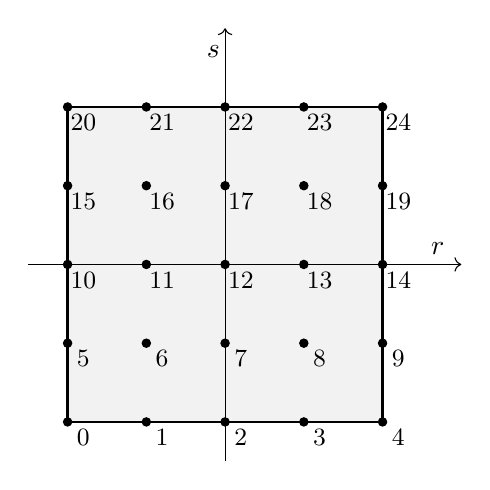
\begin{tikzpicture}
%\draw[step=0.5cm,gray,very thin] (0,0) grid (5,5); 
\draw[fill=gray!10,gray!10](1,1) rectangle (5,5);
\draw[thick] (1,1)--(5,1)--(5,5)--(1,5)--cycle;
\draw [->] (0.5,3) -- (6,3);
\draw [->] (3,0.5) -- (3,6);
\node[] at (5.7,3.2) {$r$};
\node[] at (2.85,5.7) {$s$};
\draw[black,fill=black] (1,1)   circle (1.5pt);
\draw[black,fill=black] (1,2)   circle (1.5pt);
\draw[black,fill=black] (1,3)   circle (1.5pt);
\draw[black,fill=black] (1,4)   circle (1.5pt);
\draw[black,fill=black] (1,5)   circle (1.5pt);

\draw[black,fill=black] (2,1)   circle (1.5pt);
\draw[black,fill=black] (2,2)   circle (1.5pt);
\draw[black,fill=black] (2,3)   circle (1.5pt);
\draw[black,fill=black] (2,4)   circle (1.5pt);
\draw[black,fill=black] (2,5)   circle (1.5pt);

\draw[black,fill=black] (3,1)   circle (1.5pt);
\draw[black,fill=black] (3,2)   circle (1.5pt);
\draw[black,fill=black] (3,3)   circle (1.5pt);
\draw[black,fill=black] (3,4)   circle (1.5pt);
\draw[black,fill=black] (3,5)   circle (1.5pt);

\draw[black,fill=black] (4,1)   circle (1.5pt);
\draw[black,fill=black] (4,2)   circle (1.5pt);
\draw[black,fill=black] (4,3)   circle (1.5pt);
\draw[black,fill=black] (4,4)   circle (1.5pt);
\draw[black,fill=black] (4,5)   circle (1.5pt);

\draw[black,fill=black] (5,1)   circle (1.5pt);
\draw[black,fill=black] (5,2)   circle (1.5pt);
\draw[black,fill=black] (5,3)   circle (1.5pt);
\draw[black,fill=black] (5,4)   circle (1.5pt);
\draw[black,fill=black] (5,5)   circle (1.5pt);

\node[] at (1.2,0.8) {\small $0$};
\node[] at (2.2,0.8) {\small $1$};
\node[] at (3.2,0.8) {\small $2$};
\node[] at (4.2,0.8) {\small $3$};
\node[] at (5.2,0.8) {\small $4$};

\node[] at (1.2,1.8) {\small $5$};
\node[] at (2.2,1.8) {\small $6$};
\node[] at (3.2,1.8) {\small $7$};
\node[] at (4.2,1.8) {\small $8$};
\node[] at (5.2,1.8) {\small $9$};

\node[] at (1.2,2.8) {\small $10$};
\node[] at (2.2,2.8) {\small $11$};
\node[] at (3.2,2.8) {\small $12$};
\node[] at (4.2,2.8) {\small $13$};
\node[] at (5.2,2.8) {\small $14$};

\node[] at (1.2,3.8) {\small $15$};
\node[] at (2.2,3.8) {\small $16$};
\node[] at (3.2,3.8) {\small $17$};
\node[] at (4.2,3.8) {\small $18$};
\node[] at (5.2,3.8) {\small $19$};

\node[] at (1.2,4.8) {\small $20$};
\node[] at (2.2,4.8) {\small $21$};
\node[] at (3.2,4.8) {\small $22$};
\node[] at (4.2,4.8) {\small $23$};
\node[] at (5.2,4.8) {\small $24$};

\end{tikzpicture}
\end{center}



%.....................................................................
\subsubsection{Linear basis functions for triangles in 2D ($P_1$)}\label{ss:p1}
\index{general}{$P_1$}

\begin{flushright} {\tiny {\color{gray} basis\_P1\_2D.tex}} \end{flushright}
%~~~~~~~~~~~~~~~~~~~~~~~~~~~~~~~~~~~~~~~~~~~~~~~~~~~~~~~~~~~~~~~~~~~~~~~~~~~~~~~~~~~~~~~~~~~~~~~~~~

Here we do not start from a reference element but consider instead a generic triangle:

\input{tikz/tikz_P1}

This is the simplest 2D element, which is also called linear triangular element.
Velocities (or displacements) $(u^h,v^h)$ in the element are interpolated from nodal velocities
$(u_i,v_i)$ using basis functions $\bN_i$ as follows,
\begin{small}
\[
\vec\upnu^h=
\left(
\begin{array}{c}
u^h(x,y) \\v^h(x,y)
\end{array}
\right)
=
\left(
\begin{array}{c}
\sum\limits_{i=1}^3 \bN_i(x,y) u_i \\
\sum\limits_{i=1}^3 \bN_i(x,y) v_i
\end{array}
\right)
=
\left(
\begin{array}{cccccc}
\bN_1(x,y) & 0 & \bN_2(x,y) & 0 & \bN_3(x,y) & 0\\
0 & \bN_1(x,y) & 0 & \bN_2(x,y) & 0 & \bN_3(x,y)\\
\end{array}
\right)
\cdot
\left(
\begin{array}{c}
u_1 \\ v_1 \\ u_2 \\ v_2 \\ u_3 \\ v_3
\end{array}
\right)
\]
\end{small}

For this element, we have three nodes at the vertices of the triangle, which are 
numbered around the element in the counterclockwise direction. 
Each node has two degrees of freedom (i.e. it can move in the $x$ and $y$ directions). 
The velocities $u^h$ and $v^h$ are assumed to be linear functions within the element, that is, 
\begin{eqnarray}
u^h(x,y)&=&b_1 +b_2x+b_3y \nn\\
v^h(x,y)&=&b_4 +b_5x+b_6y
\end{eqnarray}
where $b_i$ are constants to be determined and which depend on the triangle shape.
Note that the strain rate components are then given by
\begin{eqnarray}
\dot\varepsilon_{xx}(\vec\upnu)&=&b_2  \nn\\
\dot\varepsilon_{yy}(\vec\upnu)&=&b_6  \nn\\
\dot\varepsilon_{xy}(\vec\upnu)&=&(b_3+b_5)/2 \nn
\end{eqnarray}
and are constant throughout the element.

The velocities should satisfy the following six equations (when it is evaluated at a node we should 
recover the nodal velocity):
\begin{eqnarray}
u_1 &=& u^h(x_1,y_1)= b_1 + b_2x_1+b_3y_1 \nn\\
u_2 &=& u^h(x_2,y_2)= b_1 + b_2x_2+b_3y_2 \nn\\
u_3 &=& u^h(x_3,y_3)= b_1 + b_2x_3+b_3y_3 \nn\\
v_1 &=& v^h(x_1,y_1)= b_4 + b_5x_1+b_6y_1 \nn\\
v_2 &=& v^h(x_2,y_2)= b_4 + b_5x_2+b_6y_2 \nn\\
v_3 &=& v^h(x_3,y_3)= b_4 + b_5x_3+b_6y_3 \nn
\end{eqnarray}
Let us focus on the three equations with the $u$ component of the velocity.
These can be re-written:
\[
\left(
\begin{array}{c}
u_1 \\ u_2 \\ u_3  
\end{array}
\right)
=
\left(
\begin{array}{ccc}
1 & x_1 & y_1 \\
1 & x_2 & y_2 \\
1 & x_3 & y_3 \\
\end{array}
\right)
\cdot
\left(
\begin{array}{c}
b_1 \\ b_2 \\ b_3  
\end{array}
\right)
\]
In order to obtain $b_1,b_2,b_3$ we need to solve this system, or simply to compute the
inverse of the $3\times 3$ ${\bm M}$ matrix, as explained in Appendix~\ref{sec:inv3x3}.
We define $D={\rm det}({\bm M})$ and we get
\[
\left(
\begin{array}{c}
b_1 \\ b_2 \\ b_3  
\end{array}
\right)
=
\frac{1}{D}
\tilde{\bm M}
\cdot
\left(
\begin{array}{c}
u_1 \\ u_2 \\ u_3  
\end{array}
\right)
%\qquad
%{\rm and}
%\qquad
%\left(
%\begin{array}{c}
%b_4 \\ b_5 \\ b_6  
%\end{array}
%\right)
%=
%\frac{1}{D}
%\tilde{\bm M}
%\cdot
%\left(
%\begin{array}{c}
%v_1 \\ v_2 \\ v_3  
%\end{array}
%\right)
\]
The matrix $\tilde{\bm M}$ is given by:
\[
\tilde{\bm M}
%=
%\left(
%\begin{array}{ccc}
%  x_2y_3-x_3y_2  & -(y_3-y_2) &   x_3-x_2 \\
%-(x_1y_3-x_3y_1) &   y_3-y_1  & -(x_3-x_1) \\
%  x_1y_2-x_2y_1  & -(y_2-y_1) &   x_2-x_1
%\end{array}
%\right)
=
\left(
\begin{array}{ccc}
x_2y_3-x_3y_2 & x_3y_1-x_1y_3 & x_1y_2-x_2y_1 \\
y_2-y_3 & y_3-y_1  & y_1-y_2 \\
x_3-x_2 & x_1-x_3 & x_2-x_1 
\end{array}
\right)
\]
so that 
\begin{eqnarray}
b_1 &=& \frac1D [ (x_2y_3-x_3y_2)u_1 + (x_3y_1-x_1y_3)u_2 + (x_1y_2-x_2y_1)u_3 ] \nn\\
b_2 &=& \frac1D [ (y_2-y_3)u_1 + (y_3-y_1)u_2 + (y_1-y_2)u_3 ] \nn\\
b_3 &=& \frac1D [ (x_3-x_2)u_1 + (x_1-x_3)u_2 + (x_2-x_1)u_3 ]
\end{eqnarray}
We then have
\begin{eqnarray}
u^h(x,y) 
&=& b_1 + b_2 x + b_3 y \nn\\
&=&\frac1D [(x_2y_3-x_3y_2)u_1 + (x_3y_1-x_1y_3)u_2 + (x_1y_2-x_2y_1)u_3 ] \nn\\
&+&\frac1D [(y_2-y_3)u_1 + (y_3-y_1)u_2 + (y_1-y_2)u_3]x \nn\\
&+&\frac1D [(x_3-x_2)u_1 + (x_1-x_3)u_2 + (x_2-x_1)u_3]y \nn\\
&=&\frac1D [(x_2y_3-x_3y_2) + (y_2-y_3)x + (x_3-x_2)y]u_1\nn\\ 
&+&\frac1D [(x_3y_1-x_1y_3) + (y_3-y_1) x + (x_1-x_3) y]u_2 \nn\\
&+&\frac1D [(x_1y_2-x_2y_1) + (y_1-y_2) x + (x_2-x_1) y]u_3\nn\\
&=& \bN_1(x,y) u_1 + \bN_2(x,y) u_2 + \bN_3(x,y) u_3
\end{eqnarray}
with the linear basis functions are given by:
\begin{eqnarray}
\bN_1(x,y) &=& \frac{1}{D}[(x_2y_3-x_3y_2) + (y_2-y_3)x + (x_3-x_2)y] \nn\\
\bN_2(x,y) &=& \frac{1}{D}[(x_3y_1-x_1y_3) + (y_3-y_1)x + (x_1-x_3)y] \nn\\
\bN_3(x,y) &=& \frac{1}{D}[(x_1y_2-x_2y_1) + (y_1-y_2)x + (x_2-x_1)y] \nn
\end{eqnarray}
We can then easily verify that for example
\begin{eqnarray}
\bN_2(x_1,y_1)&=& \frac{1}{D}[(x_3y_1-x_1y_3) + (y_3-y_1)x_1 + (x_1-x_3)y_1] = 0 \\
\bN_2(x_2,y_2)&=& \frac{1}{D}[(x_3y_1-x_1y_3) + (y_3-y_1)x_2 + (x_1-x_3)y_2] = 1 \\
\bN_2(x_3,y_3)&=& \frac{1}{D}[(x_3y_1-x_1y_3) + (y_3-y_1)x_3 + (x_1-x_3)y_3] = 0 
\end{eqnarray}
Note that the area $A$ of the triangle is given by:
\[
A=\frac{1}{2}D = \frac{1}{2}
\left|
\begin{array}{ccc}
1 & x_1 & y_1 \\
1 & x_2 & y_2 \\
1 & x_3 & y_3 
\end{array}
\right|
\]

\noindent If we now consider the reference element in the reduced coordinates space $(r,s)$:

\input{tikz/tikz_P1ref}

The basis polynomial is then
\[
f(r,s) = a + br + cs 
\]
and the basis functions:
\begin{mdframed}[backgroundcolor=blue!5]
\begin{eqnarray}
\bN_0(r,s) &=& 1-r-s \\
\bN_1(r,s) &=& r \\
\bN_2(r,s) &=& s 
\end{eqnarray}
\end{mdframed}
Once again we can verify that $\bN_i(x_j,y_j)=\delta_{ij}$ and $\sum\limits_i \bN_i(r,s)=1$.


Coming back to the basis functions given for a generic triangle, we have
\begin{eqnarray}
\bN_1(x,y) &=& \frac{1}{D}[(x_2y_3-x_3y_2) + (y_2-y_3)x + (x_3-x_2)y] \nn\\
\bN_2(x,y) &=& \frac{1}{D}[(x_3y_1-x_1y_3) + (y_3-y_1)x + (x_1-x_3)y] \nn\\
\bN_3(x,y) &=& \frac{1}{D}[(x_1y_2-x_2y_1) + (y_1-y_2)x + (x_2-x_1)y] \nn
\end{eqnarray}
or, introducing the notations $x_{ij}=x_i-x_j$ and $y_{ij}=y_i-y_j$:
\begin{eqnarray}
\bN_1(x,y) &=& \frac{1}{D}[(x_2y_3-x_3y_2) + y_{23} x + x_{32} y] \nn\\
\bN_2(x,y) &=& \frac{1}{D}[(x_3y_1-x_1y_3) + y_{31} x + x_{13} y] \nn\\
\bN_3(x,y) &=& \frac{1}{D}[(x_1y_2-x_2y_1) + y_{12} x + x_{21} y] \nn
\end{eqnarray}
with $D=2|T|$ with $|T|$ being the area of the triangle.



The gradient matrix is then given by (see for example \cite{koko07}) 
\[
{\bm B} = 
\frac{1}{2|T|}
\begin{pmatrix}
\partial_x \bN_1 & 0 & \partial_x \bN_2 & 0 & \partial_x \bN_3 & 0 \\
0 & \partial_y \bN_1 & 0 & \partial_y \bN_2 & 0 & \partial_y \bN_3 \\
\partial_y \bN_1 & \partial_x \bN_1 &
\partial_y \bN_2 & \partial_x \bN_2 &
\partial_y \bN_3 & \partial_x \bN_3 
\end{pmatrix}
= \frac{1}{2|T|} \tilde{\bm B}
\]
with 
\[
\tilde{\bm B}=
\begin{pmatrix}
y_{23} & 0 & y_{31} & 0 & y_{12} & 0 \\
0 & x_{32} & 0 & x_{13} & 0 & x_{21} \\
x_{32} & y_{23} & x_{13} & y_{31} & x_{21} & y_{12}
\end{pmatrix}
\]

{\it What follows is written specifically for the $P_1$ element 
used in the context of elasticity and originates in \cite{koko07}.}

We can also rewrite the element displacement vector
\[
\vec{u}_e = (u_1, v_1, u_2, v_2, u_3, v_3)^T
\]
in a non-standard form
\[
\vec{u}_e = (u_1, u_2, u_3, v_1, v_2, v_3)^T
\]
Then the corresponding gradient matrix is 
\[
\tilde{\bm B}=
\begin{pmatrix}
y_{23}  & y_{31}  & y_{12} & 0 & 0 & 0 \\
0 & 0 & 0 & x_{32}  & x_{13}  & x_{21} \\
x_{32} & x_{13} & x_{21} & y_{23} &  y_{31}  & y_{12}
\end{pmatrix}
\]
We have 
\[
{\bm C} =
\begin{pmatrix}
\lambda + 2 \mu & \lambda & 0 \\
\lambda & \lambda + 2 \mu & 0 \\
0 & 0 & \mu
\end{pmatrix}
=
\begin{pmatrix}
\tilde\lambda  & \lambda & 0 \\
\lambda & \tilde\lambda  & 0 \\
0 & 0 & \mu
\end{pmatrix}
\]
Then 



\begin{landscape}
\begin{eqnarray}
&&
{\bm B}^T \cdot {\bm C} \cdot {\bm B} \nn\\
&=& \frac{1}{4|T|^2} \tilde{\bm B}^T \cdot {\bm C} \cdot \tilde{\bm B} \nn\\
&=& \frac{1}{4|T|^2} \tilde{\bm B}^T \cdot 
\begin{pmatrix}
\tilde\lambda  & \lambda & 0 \\
\lambda & \tilde\lambda  & 0 \\
0 & 0 & \mu
\end{pmatrix}
\cdot 
\begin{pmatrix}
y_{23}  & y_{31}  & y_{12} & 0 & 0 & 0 \\
0 & 0 & 0 & x_{32}  & x_{13}  & x_{21} \\
x_{32} & x_{13} & x_{21} & y_{23} &  y_{31}  & y_{12}
\end{pmatrix} \nn\\
&=& \frac{1}{4|T|^2} \tilde{\bm B}^T \cdot 
\begin{pmatrix}
\tilde\lambda y_{23} & \tilde\lambda y_{31} & \tilde\lambda y_{12} & \lambda x_{32} & \lambda x_{13} & \lambda x_{21} \\
\lambda y_{23} &  \lambda y_{31} &  \lambda y_{12} & \tilde\lambda x_{32} & \tilde\lambda x_{13} & \tilde\lambda x_{21} \\
\mu x_{32} &    \mu x_{13} & \mu x_{21} & \mu y_{23} &    \mu y_{31} & \mu y_{12}  
\end{pmatrix} \nn\\
&=&
\frac{1}{4|T|^2} 
\begin{pmatrix}
y_{23} & 0 & x_{32} \\
y_{31} & 0 & x_{13} \\
y_{12} & 0 & x_{21} \\
0 & x_{32} & y_{23} \\
0 & x_{13} & y_{31} \\
0 & x_{21} & y_{12} 
\end{pmatrix}
\cdot
\begin{pmatrix}
\tilde\lambda y_{23} & \tilde\lambda y_{31} & \tilde\lambda y_{12} & \lambda x_{32} & \lambda x_{13} & \lambda x_{21} \\
\lambda y_{23} &  \lambda y_{31} &  \lambda y_{12} & \tilde\lambda x_{32} & \tilde\lambda x_{13} & \tilde\lambda x_{21} \\
\mu x_{32} &    \mu x_{13} & \mu x_{21} & \mu y_{23} &    \mu y_{31} & \mu y_{12}  
\end{pmatrix} \nn\\
&=&
\frac{1}{4|T|^2} 
\begin{pmatrix}
\tilde\lambda y_{23}^ 2 + \mu x_{32}^2 &
\tilde\lambda y_{23}y_{31} + \mu x_{32}x_{13} &
\tilde\lambda y_{23}y_{12} + \mu x_{32}x_{21} &
\lambda y_{23}x_{32} + \mu x_{32}y_{23} &
\lambda y_{23}x_{13} + \mu x_{32}y_{31} &
\lambda y_{23}x_{21} + \mu x_{32}y_{12}  
\\
\tilde\lambda y_{31}y_{23} + \mu x_{13}x_{32} &
\tilde\lambda y_{31}^2 + \mu x_{13}^2 &
\tilde\lambda y_{31}y_{12} + \mu x_{13}x_{21} &
\lambda y_{31}x_{32} + \mu x_{13}y_{23}  &
\lambda y_{31}x_{13} + \mu x_{13}y_{31}  &
\lambda y_{31}x_{21} + \mu x_{13}y_{12}  
\\
\tilde\lambda y_{12}y_{23} + \mu x_{21}x_{32} &
\tilde\lambda y_{12}y_{31} + \mu x_{21}x_{13} &
\tilde\lambda y_{12}^2 + \mu x_{21}^2 &
\lambda y_{12}x_{32} + \mu x_{21}y_{23}  &
\lambda y_{12}x_{13} + \mu x_{21}y_{31}  &
\lambda y_{12}x_{21} + \mu x_{21}y_{12}  
\\
. & .& . &
\tilde\lambda x_{32}^2 + \mu y_{23}^2 &
\tilde\lambda x_{32}x_{13} + \mu y_{23}y_{31} &
\tilde\lambda x_{32}x_{21} + \mu y_{23}y_{12} 
\\
. & . & . & 
\tilde\lambda x_{13}x_{32} + \mu y_{31}y_{23} &
\tilde\lambda x_{13}^2 + \mu y_{31}^2 &
\tilde\lambda x_{13}x_{21} + \mu y_{31}y_{12} 
\\
. & . & . &
\tilde\lambda x_{21}x_{32} + \mu y_{12}y_{23} &
\tilde\lambda x_{21}x_{13} + \mu y_{12}y_{31} &
\tilde\lambda x_{21}^2 + \mu y_{12}^2 
\end{pmatrix} 
\nn\\
&=& \frac{1}{4|T|^2} 
\begin{pmatrix}
\K_{xx} & \K_{xy} \\
\K_{yx} & \K_{yy}
\end{pmatrix}
\end{eqnarray}
\end{landscape}

with
\begin{eqnarray}
\K_{xx} &=&  
\begin{pmatrix}
\tilde\lambda y_{23}^ 2 + \mu x_{32}^2 &
\tilde\lambda y_{23}y_{31} + \mu x_{32}x_{13} &
\tilde\lambda y_{23}y_{12} + \mu x_{32}x_{21} \\
\tilde\lambda y_{31}y_{23} + \mu x_{13}x_{32} &
\tilde\lambda y_{31}^2 + \mu x_{13}^2 &
\tilde\lambda y_{31}y_{12} + \mu x_{13}x_{21} \\
\tilde\lambda y_{12}y_{23} + \mu x_{21}x_{32} &
\tilde\lambda y_{12}y_{31} + \mu x_{21}x_{13} &
\tilde\lambda y_{12}^2 + \mu x_{21}^2 &
\end{pmatrix}
\nn\\
\K_{yy} &=&  
\begin{pmatrix}
\tilde\lambda x_{32}^2 + \mu y_{23}^2 &
\tilde\lambda x_{32}x_{13} + \mu y_{23}y_{31} &
\tilde\lambda x_{32}x_{21} + \mu y_{23}y_{12} 
\\
\tilde\lambda x_{13}x_{32} + \mu y_{31}y_{23} &
\tilde\lambda x_{13}^2 + \mu y_{31}^2 &
\tilde\lambda x_{13}x_{21} + \mu y_{31}y_{12} 
\\
\tilde\lambda x_{21}x_{32} + \mu y_{12}y_{23} &
\tilde\lambda x_{21}x_{13} + \mu y_{12}y_{31} &
\tilde\lambda x_{21}^2 + \mu y_{12}^2 
\end{pmatrix}
\nn\\
\K_{xy} = \K_{yx}^T &=&
\begin{pmatrix}
\lambda y_{23}x_{32} + \mu x_{32}y_{23} &
\lambda y_{23}x_{13} + \mu x_{32}y_{31} &
\lambda y_{23}x_{21} + \mu x_{32}y_{12}  
\\
\lambda y_{31}x_{32} + \mu x_{13}y_{23}  &
\lambda y_{31}x_{13} + \mu x_{13}y_{31}  &
\lambda y_{31}x_{21} + \mu x_{13}y_{12}  
\\
\lambda y_{12}x_{32} + \mu x_{21}y_{23}  &
\lambda y_{12}x_{13} + \mu x_{21}y_{31}  &
\lambda y_{12}x_{21} + \mu x_{21}y_{12}  
\end{pmatrix}
\end{eqnarray}

If we now introduce the vectors
\[
\vec{x} = 
\begin{pmatrix}
x_{32} \\ x_{13} \\ x_{21} 
\end{pmatrix}
\qquad \text{and}
\qquad
\vec{y}=
\begin{pmatrix}
y_{23} \\ y_{31} \\ y_{12}
\end{pmatrix}
\]
then 
\begin{eqnarray}
\K_{xx} &=&  (\lambda+2\mu) \vec{y}\vec{y}^T + \mu \vec{x}\vec{x}^T \nn\\
\K_{yy} &=&  (\lambda+2\mu) \vec{x}\vec{x}^T + \mu \vec{y}\vec{y}^T \nn\\
\K_{xy} &=& \lambda \vec{y}\vec{x}^T  + \mu \vec{x} \vec{y}^T \nn
\end{eqnarray}

In the end 
\begin{eqnarray}
\K 
&=& \int_T {\bm B}^T \cdot {\bm C} \cdot {\bm B} dV \nn\\
&=& \int_T \frac{1}{4|T|^2} \tilde{\bm B}^T \cdot {\bm C} \cdot \tilde {\bm B} dV \nn\\
&=&  \frac{1}{4|T|^2}  \tilde{\bm B}^T \cdot {\bm C} \cdot \tilde {\bm B} \int_T dV \nn\\
&=&  \frac{1}{4|T|}  \tilde{\bm B}^T \cdot {\bm C} \cdot \tilde {\bm B} 
\end{eqnarray}

This means that one can compute elemental matrices for each triangle
without using Gauss integration (as long as the coefficients are 
constant within the triangle).

Whether the same approach can be taken in 3d needs to be looked at ...











%.....................................................................
\subsubsection{Linear basis functions for quadrilaterals in 2D ($P_1$)}\label{ss:lbfq2D}
\index{general}{$P_1$}

\begin{flushright} {\tiny {\color{gray} basis\_Pm1\_2D.tex}} \end{flushright}
%~~~~~~~~~~~~~~~~~~~~~~~~~~~~~~~~~~~~~~~~~~~~~~~~~~~~~~~~~~~~~~~~~~~~~~~~~~~~~~~~~~~~~~~~~~~~~~~~~~

On the reference element $\Omega=[-1,1]\times[-1,1]$ we have three nodes placed as follows:

\input{tikz/tikz_pm1_2D}

Let us assume that the function $f(r,s)$ is to be approximated on $[-1,1]\times[-1,1]$ by 
\[
f^h(r,s)=a+br+cs
\]
Note that this is a linear function, not a bilinear one. 
The function $f^h$ then must fulfill:
\begin{eqnarray}
f^h(r_1,s_1)&=&a \;\;\;\;\;\; =f_1    \nn\\
f^h(r_2,s_2)&=&a+\frac{b}{2}=f_2 \nn\\
f^h(r_3,s_3)&=&a+\frac{c}{2}=f_3 \nn
\end{eqnarray}
This leads to : 
\[
a=f_1
\quad
\quad
b=2(f_2-f_1)
\quad
\quad
c=2(f_3-f_1)
\]
Then
\[
f(r,s)=f_1 + 2(f_2-f_1) r + 2(f_3-f_1) s
\]
or, 
\[
f(r) = \sum_{i=1}^3 N_i(r,s) f_i
\]
with
\begin{mdframed}[backgroundcolor=blue!5]
\begin{eqnarray}
\bN_1(r) &=& 1-2(r+s)  \nonumber\\
\bN_2(r) &=& 2r   \nonumber\\
\bN_3(r) &=& 2s
\end{eqnarray}
\end{mdframed}

Note that we could also have placed the nodes at a different location: 

\input{tikz/tikz_pm1_2D_bis}

and we would then have
\begin{mdframed}[backgroundcolor=blue!5]
\begin{eqnarray}
\bN_1(r) &=& 1-r-s  \nonumber\\
\bN_2(r) &=& r   \nonumber\\
\bN_3(r) &=& s
\end{eqnarray}
\end{mdframed}








%.....................................................................
\subsubsection{Enriched linear basis functions in triangles ($P_1^+$)}
\index{general}{$P_1^+$}

As we will see in Section~\ref{pair:mini} the above $P_1$ can be enriched 
with a so-called bubble function.
The \index{general}{Bubble Function} bubble function of the MINI element 
is described in \cite{arbf84} as being $\lambda_1\lambda_2\lambda_3$
where $\lambda_i$ are the so-called barycentric 
coordinates\footnote{\url{https://en.wikipedia.org/wiki/Barycentric\_coordinate\_system }}.
\index{general}{Barycentric Coordinates}

\begin{eqnarray}
\lambda_1 &=& \frac{(y2-y3)(x-x3)+(x3-x2)(y-y3)}{(y2-y3)(x1-x3)+(x3-x2)(y1-y3)} \nn\\
\lambda_2 &=& \frac{(y3-y1)(x-x3)+(x1-x3)(y-y3)}{(y2-y3)(x1-x3)+(x3-x2)(y1-y3)} \nn\\
\lambda_3 &=& 1-\lambda_1-\lambda_2 \nn
\end{eqnarray}

\begin{center}
\includegraphics[width=12cm]{images/mini/minielement2}\\
{\small representation of the element in the real coordinate system $(x,y)$
and in the reduced coordinate system $(r,s)$}
\end{center}

\begin{center}
\includegraphics[width=5cm]{images/mini/barycoord}\\
{\small Barycentric coordinates ($\lambda _{1},\lambda _{2},\lambda _{3}$) on an equilateral triangle and on a right triangle.}
\end{center}

In the reference triangle, the barycentric coordinates write
\begin{eqnarray}
\lambda_1 &=& \frac{(s_2-s_3)(r-r_3)+(r_3-r_2)(s-s_3)}{(s_2-s_3)(r_1-r_3)+(r_3-r_2)(s_1-s_3)} = \frac{(-1)(r)+(-1)(s-1)}{(-1)(0)+(-1)(-1)} = -r-s+1  \nn\\
\lambda_2 &=& \frac{(s3-s1)(r-r3)+(r1-r3)(s-s3)}{(s2-s3)(r1-r3)+(r3-r2)(s1-s3)} = \frac{(1)(r)+(0)(s-1)}{(-1)(0)+(-1)(-1)} = r \nn\\
\lambda_3 &=& 1-\lambda_1-\lambda_2 = 1 - (-r-s+1) - r = s \nn
\end{eqnarray}
As we have seen before the bubble function is given by $\lambda_1\lambda_2\lambda_3 = (1-r-s)rs$
and the polynomial form for the basis functions is given by:
\[
f(r,s) =a+br+cs + d (1-r-s)rs
\]
Setting the location of the bubble at $r=s=1/3$, i.e. $\lambda_1\lambda_2\lambda_3 = 1/3$, 
we then have 
\begin{eqnarray}
f(r_1,s_1)&=&f_1 = a+br_1+cs_1 + d (1-r_1-s_1)r_1s_1 = a \nn\\
f(r_2,s_2)&=&f_2 = a+br_2+cs_2 + d (1-r_2-s_2)r_2s_2 = a + b \nn\\
f(r_3,s_3)&=&f_3 = a+br_3+cs_3 + d (1-r_3-s_3)r_3s_3 = a + c \nn\\
f(r_4,s_4)&=&f_4 = a+br_4+cs_4 + d (1-r_4-s_4)r_4s_4 = a + \frac{b}{3} + \frac{c}{3} + \frac{1}{27} \nn
\end{eqnarray}
where point 4 is the location of the bubble.
This yields
\[
a=f_1 
\quad\quad\qquad
b=f_2-a = f_2-f_1
\quad\quad\qquad
c=f_3-a = f_3-f_1
\]
and
\[
d=27(f_4-a-\frac{b}{3} - \frac{c}{3}) = 27 (f_4 - f_1 - \frac{f_2-f_1}{3} - \frac{f_3-f_1}{3} )
=27(f_4 - \frac{f_1}{3}  - \frac{f_2}{3}  - \frac{f_3}{3} )
\] 

Finally
\begin{eqnarray}
f(r,s) 
&=&a+br+cs + d (1-r-s)rs \nn\\
&=& f_1 + (f_2-f_1)r + (f_3-f_1)s + 27(f_4 - \frac{f_1}{3}  - \frac{f_2}{3}  - \frac{f_3}{3} ) (1-r-s)rs \nn\\
&=& [1-r-s-9(1-r-s)rs] f_1 + [r-9(1-r-s)rs ]f_2 + [s-9(1-r-s)rs ]f_3 + [27(1-r-s)rs]f_4 \nn
\end{eqnarray}
so that 
\[
f(r,s)=\sum_{i=1}^4 N_i(r,s) f_i
\]
with 
%\begin{mdframed}[backgroundcolor=blue!15]
\begin{eqnarray}
N_1(r,s) &=& 1-r-s-9(1-r-s)rs \nn\\
N_2(r,s) &=& r-9(1-r-s)rs \nn\\
N_3(r,s) &=& s-9(1-r-s)rs \nn\\
N_4(r,s) &=& 27(1-r-s)rs \nn
\end{eqnarray}
%\end{mdframed}
It is trivial to verify that $\sum_i N_i =1$ for all values of $r,s$
and the gradients of the basis functions are:
\begin{eqnarray}
\frac{\partial N_1}{\partial r}(r,s) &=& -1 - 9(1-2r-s)s \\ 
\frac{\partial N_2}{\partial r}(r,s) &=&  +1 - 9(1-2r-s)s \\ 
\frac{\partial N_3}{\partial r}(r,s) &=&  - 9(1-2r-s)s \\ 
\frac{\partial N_4}{\partial r}(r,s) &=&  27(1-2r-s)s \\ 
\\
\frac{\partial N_1}{\partial s}(r,s) &=& -1 - 9(1-r-2s)r \\ 
\frac{\partial N_2}{\partial s}(r,s) &=&    - 9(1-r-2s)r \\ 
\frac{\partial N_3}{\partial s}(r,s) &=& +1 - 9(1-r-2s)r \\ 
\frac{\partial N_4}{\partial s}(r,s) &=&     27(1-r-2s)r 
\end{eqnarray}

We have two coordinate systems for the element: the global coordinates $(x,y)$ 
and the natural coordinates $(r,s)$. Inside the element, the relation between the two is given by
\begin{eqnarray}
x &=& N_1 x_1 + N_2 x_2 + N_3 x_3 + N_4 x_4 = \sum_i N_i(r,s) x_i\nn\\
y &=& N_1 y_1 + N_2 y_2 + N_3 y_3 + N_4 y_4 = \sum_i N_i(r,s) y_i
\end{eqnarray}
or,
\begin{eqnarray}
x &=& [ 1-r-s-9(1-r-s)rs] x_1 + [r-9(1-r-s)rs] x_2 + [s-9(1-r-s)rs] x_3 + [27(1-r-s)rs] x_4 \nn\\
&=& x_1 -r (x_1-x_2) -s (x_1-x_3) + (1-r-s)rs (-9 x_1 - 9 x_2  -9 x_3 +27 x_4)  \nn\\
&=& x_1 -r (x_1-x_2) -s (x_1-x_3) + (1-r-s)rs (-9 x_1 - 9 x_2  -9 x_3 +27 (x_1+x_2+x_3)/3) \nn\\ 
&=& x_1 -r (x_1-x_2) -s (x_1-x_3) \nn\\ 
&=& x_1 -r x_{12} -s x_{13} \nn\\ 
y &=& [ 1-r-s-9(1-r-s)rs] y_1 + [r-9(1-r-s)rs] y_2 + [s-9(1-r-s)rs] y_3 + [27(1-r-s)rs] y_4 \nn\\
&=& y_1 -r (y_1-y_2) -s (y_1-y_3) + (1-r-s)rs (-9 y_1 - 9 y_2  -9 y_3 +27 y_4)  \nn\\
&=& y_1 -r (y_1-y_2) -s (y_1-y_3) + (1-r-s)rs (-9 y_1 - 9 y_2  -9 y_3 +27 (y_1+y_2+y_3)/3) \nn\\ 
&=& y_1 -r (y_1-y_2) -s (y_1-y_3) \nn \\
&=& y_1 -r y_{12} -s y_{13} \nn 
\end{eqnarray}




























%%%%%%%%%%%%%%%%%%%%%%%%%%%%%%%%%%%%
\subsubsection{Quadratic basis functions for triangles in 2D ($P_2$)}
\index{general}{$P_2$}

\begin{verbatim}
2            
|\
| \        (r_0,s_0)=(0,0) (r_3,s_3)=(1/2,0)
5   4      (r_1,s_1)=(1,0) (r_4,s_4)=(1/2,1/2)
|     \    (r_2,s_2)=(0,1) (r_5,s_5)=(0,1/2)
|      \ 
0===3===1
\end{verbatim}
The basis polynomial is then
\[
f(r,s) = c_1 + c_2 r + c_3 s + c_4  r^2 + c_5 rs  + c_6 s^2
\]
We have 
\begin{eqnarray}
f_1 = f(r_1,s_1) &=& c_1 \nonumber\\
f_2 = f(r_2,s_2) &=& c_1 + c_2 + c_4\nonumber\\
f_3 = f(r_3,s_3) &=& c_1 + c_3 + c_6\nonumber\\
f_4 = f(r_4,s_4) &=& c_1 + c_2/2 + c_4/4\nonumber\\
f_5 = f(r_5,s_5) &=& c_1 + c_2/2 + c_3/2 \nonumber\\
                 &+& c_4/4 + c_5/4 + c_6/4\nonumber\\
f_6 = f(r_6,s_6) &=& c_1 + c_3/2 + c_6/4\nonumber
\end{eqnarray}

This can be cast as ${\bm f}={\bm A}\cdot {\bm c}$ where ${\bm A}$ is a 6x6 matrix:
\[
{\bm A}=
\left(
\begin{array}{cccccc}
1&0   &  0  & 0   & 0   & 0\\
1&1   &  0  & 1   & 0   & 0\\
1&0   &  1  & 0   & 0   & 1\\
1&1/2 &  0  & 1/4 & 0   & 0\\
1&1/2 &  1/2& 1/4 & 1/4 & 1/4\\
1&0   &  1/2& 0   & 0   & 1/4
\end{array}
\right)
\]
It is rather trivial to compute the inverse of this matrix:
\[
{\bm A}^{-1}=
\left(
\begin{array}{cccccc}
1  & 0 & 0  & 0  & 0 & 0  \\
-3 & -1& 0  & 4  & 0 & 0 \\
-3 & 0 & -1 & 0  & 0 & 4 \\
2  & 2 & 0  & -4 & 0 & 0  \\
4  & 0 & 0  & -4 & 4 & -4 \\
2  & 0 & 2  & 0  & 0 & -4
\end{array}
\right)
\]
In the end, one obtains:
\begin{eqnarray}
f(r,s) 
&=& f_1 + (-3f_1-f_2+4f_4) r + (-3f_1-f_3+4f_6)s \nonumber\\
&& +(2f_1+2f_2-4f_4)r^2 + (4f_1-4f_4+4f_5-4f_6) rs \nn\\
&&+ (2f_1+2f_3-4f_6)s^2 \nonumber\\
&=& \sum_{i=1}^6 N_i(r,s) f_i
\end{eqnarray}
with
\begin{mdframed}[backgroundcolor=blue!5]
\begin{eqnarray}
N_1(r,s) &=& 1-3r-3s+2r^2+4rs+2s^2 \nonumber\\
N_2(r,s) &=& -r+2r^2 \nonumber\\
N_3(r,s) &=& -s+2s^2 \nonumber\\
N_4(r,s) &=& 4r-4r^2-4rs \nonumber\\
N_5(r,s) &=& 4rs \nonumber\\
N_6(r,s) &=& 4s-4rs-4s^2 \nonumber
\end{eqnarray}
\end{mdframed}

The derivatives are as follows:
\begin{eqnarray}
\frac{\partial N_1}{\partial r}(r,s) &=&  -3+4r+4s \nn\\ 
\frac{\partial N_2}{\partial r}(r,s) &=&  -1+4r\nn\\ 
\frac{\partial N_3}{\partial r}(r,s) &=&  0\nn\\ 
\frac{\partial N_4}{\partial r}(r,s) &=&  4-8r-4s\nn\\ 
\frac{\partial N_5}{\partial r}(r,s) &=&  4s\nn\\ 
\frac{\partial N_6}{\partial r}(r,s) &=&  -4s\nn
\end{eqnarray}

\begin{eqnarray}
\frac{\partial N_1}{\partial s}(r,s) &=&  -3+4r+4s\nn\\ 
\frac{\partial N_2}{\partial s}(r,s) &=&  0\nn\\ 
\frac{\partial N_3}{\partial s}(r,s) &=&  -1+4s\nn\\ 
\frac{\partial N_4}{\partial s}(r,s) &=&  -4r\nn\\ 
\frac{\partial N_5}{\partial s}(r,s) &=&  4r\nn\\ 
\frac{\partial N_6}{\partial s}(r,s) &=&  4-4r-8s\nn
\end{eqnarray}



%.....................................................................
\subsubsection{Enriched quadratic basis functions in triangles ($P_2^+$)}
\index{general}{$P_2^+$}

This is used by the Crouzeix-Raviart element, see Section~\ref{sec:crouzeix-raviart}. 
\index{general}{Crouzeix-Raviart}

\begin{verbatim}
03             (r_1,s_1)=(0,0)
||\\           (r_2,s_2)=(1,0)
|| \\          (r_3,s_3)=(0,1)
||  \\         (r_4,s_4)=(1/2,0)
06   05        (r_5,s_5)=(1/2,1/2)
|| 07 \\       (r_6,s_6)=(0,1/2)
||     \\      (r_7,s_7)=(1/3,1/3)
01==04==02    
\end{verbatim}

The basis functions are given by:
\todo[inline]{find reference}

\begin{mdframed}[backgroundcolor=blue!5]
\begin{eqnarray}
N_1(r,s) &=&  (1-r-s)(1-2r-2s+ 3rs) \\
N_2(r,s) &=& r (2 r -1 + 3s-3rs-3s^2 ) \\
N_3(r,s) &=& s (2s -1 + 3r-3r^2-3rs )\\
N_4(r,s) &=& 4(1-r-s)r(1 -3s ) \\
N_5(r,s) &=& 4rs [-2+3r+3s]\\
N_6(r,s) &=& 4(1-r-s)s(1-3r)\\
N_7(r,s) &=& 27 (1-r-s)rs 
\end{eqnarray}
\end{mdframed}
It is then easy to verify that for all basis functions we have 
$N_i(r_j,s_j)=\delta_{ij}$ where $j$ denotes one of the seven nodes. 

The derivatives are as follows:
\begin{eqnarray}
\frac{\partial N_1}{\partial r}(r,s) &=& r(4-6s)-3s^2+7s-3\\
\frac{\partial N_2}{\partial r}(r,s) &=& r(4-6s)-3s^2+3s-1\\
\frac{\partial N_3}{\partial r}(r,s) &=& -3s(2r+s-1)  \\
\frac{\partial N_4}{\partial r}(r,s) &=& 4(3s-1)(2r+s-1) \\
\frac{\partial N_5}{\partial r}(r,s) &=& 4s(6r+3s-2) \\
\frac{\partial N_6}{\partial r}(r,s) &=& 4s(6r+3s-4)\\
\frac{\partial N_7}{\partial r}(r,s) &=& -27s(2r+s-1)
\end{eqnarray}

\begin{eqnarray}
\frac{\partial N_1}{\partial s}(r,s) &=& -3r^2+r(7-6s)+4s-3\\
\frac{\partial N_2}{\partial s}(r,s) &=& -3r(r+2s-1)\\
\frac{\partial N_3}{\partial s}(r,s) &=& -3r^2+r(3-6s)+4s-1 \\
\frac{\partial N_4}{\partial s}(r,s) &=& 4r(3r+6s-4)  \\
\frac{\partial N_5}{\partial s}(r,s) &=& 4r(3r+6s-2) \\
\frac{\partial N_6}{\partial s}(r,s) &=& 4(3r-1)(r+2s-1)\\
\frac{\partial N_7}{\partial s}(r,s) &=& -27r(r+2s-1)
\end{eqnarray}


Note that the basis functions can also be expressed as a function of the barycentric coordinates, 
as in the MILAMIN code \cite{daks08} or in Cuvelier \etal, 1986 \cite{cuss86}\footnote{Note
that the numbering of the nodes in the book is different with respect to the one above. }

\begin{verbatim}
03          
||\\        
|| \\       
||  \\      
05   04     
|| 07 \\    
||     \\   
01==06==02    
\end{verbatim}

\begin{eqnarray}
N_1(\lambda_1,\lambda_2,\lambda_3) &=& \eta_1(2\eta_1-1)+ 3\eta_1\eta_2\eta_3\\
N_2(\lambda_1,\lambda_2,\lambda_3) &=& \eta_2(2\eta_2-1)+ 3\eta_1\eta_2\eta_3\\
N_3(\lambda_1,\lambda_2,\lambda_3) &=& \eta_3(2\eta_3-1)+ 3\eta_1\eta_2\eta_3\\
N_4(\lambda_1,\lambda_2,\lambda_3) &=& 4\eta_2\eta_3 - 12\eta_1\eta_2\eta_3\\
N_5(\lambda_1,\lambda_2,\lambda_3) &=& 4\eta_1\eta_3 - 12\eta_1\eta_2\eta_3\\
N_6(\lambda_1,\lambda_2,\lambda_3) &=& 4\eta_1\eta_2 - 12\eta_1\eta_2\eta_3\\
N_7(\lambda_1,\lambda_2,\lambda_3) &=& 27\eta_1\eta_2\eta_3 
\end{eqnarray}

\todo[inline]{
VERIFY that when $\eta_1=1-r-s$, $\eta_2=r$ and $\eta_3=s$ we find the above $r,s$ basis functions
}


%1-4*eta1+3*eta1*eta3-3*eta2*eta3 ...
%-1+4*eta2+3*eta1*eta3-3*eta2*eta3 ...
%3*eta1*eta3-3*eta2*eta3 ...
%4*eta3+12*eta2*eta3-12*eta1*eta3 ...
%-4*eta3+12*eta2*eta3-12*eta1*eta3 ...
%4*eta1-4*eta2+12*eta2*eta3-12*eta1*eta3 ...
%-27*eta2*eta3+27*eta1*eta3

%1-4*eta1+3*eta1*eta2-3*eta2*eta3 ...
%+3*eta1*eta2-3*eta2*eta3 ...
%-1+4*eta3+3*eta1*eta2-3*eta2*eta3 ...
%4*eta2-12*eta1*eta2+12*eta2*eta3 ...
%4*eta1-4*eta3-12*eta1*eta2+12*eta2*eta3 ...
%-4*eta2-12*eta1*eta2+12*eta2*eta3 ...
%27*eta1*eta2-27*eta2*eta3];  







%%%%%%%%%%%%%%%%%%%%%%%%%%%%%%%%%%%%
\subsubsection{Cubic basis functions for triangles ($P_3$)}
\index{general}{$P_3$}

\begin{verbatim}
2
|\          (r_0,s_0)=(0,0)   (r_5,s_5)=(2/3,1/3)
|  \        (r_1,s_1)=(1,0)   (r_6,s_6)=(1/3,2/3)
7   6       (r_2,s_2)=(0,1)   (r_7,s_7)=(0,2/3)
|    \      (r_3,s_3)=(1/3,0) (r_8,s_8)=(0,1/3)
8  9   5    (r_4,s_4)=(2/3,0) (r_9,s_9)=(1/3,1/3)
|       \ 
0==3==4==1
\end{verbatim}
The basis polynomial is then
\[
f(r,s) = c_1 + c_2r + c_3s + c_4 r^2 + c_5 rs + c_6 s^2 + c_7 r^3 +c_8 r^2s + c_9 rs^2 + c_{10}s^3
\]
\begin{eqnarray}
N_0(r,s) &=& \frac{9}{2}(1-r-s)\left(\frac13-r-s\right)\left(\frac23-r-s\right) \\
N_1(r,s) &=& \frac{9}{2}r\left(r-\frac13\right)\left(r-\frac23 \right) \\
N_2(r,s) &=& \frac{9}{2}s\left(s-\frac13\right)\left(s-\frac23\right) \\
N_3(r,s) &=& \frac{27}{2}(1-r-s)r \left(\frac23-r-s\right) \\
N_4(r,s) &=& \frac{27}{2}(1-r-s)r\left(r-\frac13\right) \\
N_5(r,s) &=& \frac{27}{2}rs\left(r-\frac13\right) \\
N_6(r,s) &=& \frac{27}{2}rs\left(r-\frac23\right) \\
N_7(r,s) &=& \frac{27}{2}(1-r-s)s\left(s-\frac13\right) \\
N_8(r,s) &=& \frac{27}{2}(1-r-s)s \left(\frac23-r-s\right) \\
N_9(r,s) &=& 27 rs(1-r-s)
\end{eqnarray}



%..........................................................................
\subsubsection{Enriched linear basis functions in quadrilaterals ($Q_1^+$) -WIP} \label{ss:quadmini}
\index{general}{$Q_1^+$}

\begin{verbatim}
4===========3
|           |   (r_1,s_1)=(-1,-1)
|           |   (r_2,s_2)=(1,-1)
|     5     |   (r_3,s_3)=(1,1)
|           |   (r_4,s_4)=(-1,1)
|           |   (r_5,s_5)=(0,0)
1===========2
\end{verbatim}

\begin{itemize}
\item 
In Bai (1997) \cite{bai97}: "It is well known that the equal-order bilinear velocity-bilinear 
continuous pressure element - the $Q_1\times Q_1$, element - exhibits a certain spurious pressure mode.
In the paper we propose a new stabilized $Q_1\times Q_1$ combination for the velocity and
pressure with three internal degrees of freedom added to the velocity space, that is, one degree of
freedom for each component of the velocity and one degree of freedom shared by both components of
the velocity."

Two versions are proposed, if I understand it correctly.
The first one is given in Eq.~7 (three extra dofs: $u_5$, $v_5$, $w$):
\begin{eqnarray}
u^h(r,s) &=& \sum_{i=1}^4 N_i (r,s) u_i + \left[ u_5 - \frac{w}{4}(1-s) \right] (1-r^2)(1-s^2) \nonumber\\
v^h(r,s) &=& \sum_{i=1}^4 N_i (r,s) v_i + \left[ v_5 - \frac{w}{4}(1-r) \right] (1-r^2)(1-s^2) 
\end{eqnarray}
The second one in Eq.23 (four extra dofs: $u_5$, $v_5$, $u_6$, $v_6$):
\begin{eqnarray}
u^h(r,s) &=& \sum_{i=1}^4 N_i (r,s) u_i + \left[ u_5 +u_6(r+s) \right] (1-r^2)(1-s^2) \nonumber\\
v^h(r,s) &=& \sum_{i=1}^4 N_i (r,s) v_i + \left[ v_5 +v_6(r+s) \right] (1-r^2)(1-s^2) 
\end{eqnarray}

\item In Franca \etal (2007) \cite{fros07}: 
"Stabilized finite element method for Stokes equations with piecewise continuous 
bilinear approximations for both velocity and pressure variables. The velocity
field is enriched with piecewise polynomial bubble functions with null average at element
edges."

It looks like they are proposing (see their Eq.~2.6):
\begin{eqnarray}
u^h(r,s) &=& \sum_{i=1}^4 N_i (r,s) u_i + (\alpha + \gamma s)\frac{1}{2}(r^2+s^2-\frac43) \nn\\ 
v^h(r,s) &=& \sum_{i=1}^4 N_i (r,s) v_i + (\beta + \gamma r) \frac{1}{2}(r^2+s^2-\frac43)  
\end{eqnarray}

\item In Kwon \& Park \cite{kwpa14}: 
"We introduce a new stable MINI-element pair for incompressible Stokes equations on
quadrilateral meshes, which uses the smallest number of bubbles for the velocity. The pressure is 
discretized with the $P_1$-midpoint-edge-continuous elements and each component of the velocity field is
done with the standard $Q_1$-conforming elements enriched by one bubble a quadrilateral."

\item  In Lamichhane (2017) \cite{lami17}: "We consider a quadrilateral MINI
finite element for approximating the solution
of Stokes equations using a quadrilateral mesh. We use the standard bilinear finite
element space enriched with element-wise defined bubble functions for the velocity
and the standard bilinear finite element space for the pressure space. With a simple
modification of the standard bubble function we show that a single bubble function is
sufficient to ensure the inf-sup condition.
This is a refinement of \cite{bai97} where the author enriches the velocity space with
more than a single vector bubble function per element. In this article we show that 
with a small modification of the standard bubble function we can get the stability just 
by using a single vector bubble function per element."

\input{lamichhane2D}

\end{itemize}


\Literature Mons \& Roge (1992) \cite{moro92}, 
Li \etal (2009) \cite{lihc09}, Knobloch \& Tobiska (2000) \cite{knto00}, 
Franca \etal (1993) \cite{frha93}, Idelsohn \etal (1995) \cite{idsn95}.





\newpage
%-----------------------------------------------------------------
\subsubsection{The rotated $Q_1$} \label{ss:rq1}
\index{general}{$\tilde{Q}_1$}

The nodes are not on the corners of the element but in the middle of the
element edges:

\begin{flushright} {\tiny {\color{gray} (tikz\_RTQ1P0.tex)}} \end{flushright}
%~~~~~~~~~~~~~~~~~~~~~~~~~~~~~~~~~~~~~~~~~~~~~~~~~~~~~~~~~~~~~~~~~~~~~~~~~~~~~~~~~~~~~~~~~~~~~~~~~~

\begin{center}
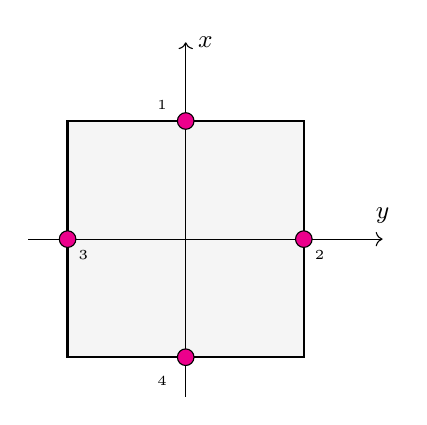
\begin{tikzpicture}
%\draw[step=1cm,gray,very thin] (0,0) grid (8,8); %background grid

\draw[thick,fill=gray!8] (1,1) -- (4,1) -- (4,4) -- (1,4) -- cycle;

\node[] at (1.2,2.3) {\tiny 3};
\node[] at (4.2,2.3) {\tiny 2};
\node[] at (2.2,.7) {\tiny 4};
\node[] at (2.2,4.2) {\tiny 1};

\draw[->] (0.5,2.5)--(5,2.5);
\draw[->] (2.5,0.5)--(2.5,5);

\draw[black,fill=magenta] (1,2.5)   circle (3pt);
\draw[black,fill=magenta] (4,2.5)   circle (3pt);
\draw[black,fill=magenta] (2.5,1)   circle (3pt);
\draw[black,fill=magenta] (2.5,4)   circle (3pt);

\node[] at (5,2.8) {\small $y$};
\node[] at (2.75,5) {\small $x$};
\end{tikzpicture}
\end{center}




\begin{verbatim}
+======3======+
|             |
|      s      |
|      |      |
4      +--r   2
|             |
|             |
|             |
+======1======+
\end{verbatim}

There are two types of basis functions: the Middle Point (MP) variant
such that $N_i({\bm r}_j)=\delta_{ij}$ and the Mid Value (MV) variant
such that $\frac{1}{|\Gamma_i|} \int_{\Gamma_i} N_j d\Gamma = \delta_{ij}$.

%.............................................
\paragraph{The Middle Point (MP) variant}. 
We have $\tilde{Q}_1=span \{ 1,r,s,r^2-s^2 \}$
so a function $f \in \tilde{Q}_1$  is such that 
\begin{equation}
f(r,s)= a + b r + c s + d(r^2-s^2 )
\label{nonpsf}
\end{equation}

This function must be so that 
\begin{eqnarray}
f_1 &=& f(r=0 ,s=-1) = a -c -d \\
f_2 &=& f(r=+1,s=0)  = a +b +d \\
f_3 &=& f(r=0 ,s=+1) = a +c -d \\
f_4 &=& f(r=-1,s=0)  = a -b +d 
\end{eqnarray}
and then 
\[
\left(
\begin{array}{c}
f_A \\ f_b \\ f_C \\ f_D
\end{array}
\right)
=
\left(
\begin{array}{cccc}
1 &0 &-1 &-1 \\
1 &1 &0 &1 \\
1 &0 &1 &-1 \\
1 &-1 &0 &1
\end{array}
\right)
\left(
\begin{array}{c}
a \\ b \\ c \\ d
\end{array}
\right)
\]
This system can easily be solved, $a,b,c,d$ are then replaced in Eq.~\eqref{nonpsf},
which yields 
\begin{eqnarray}
f(r,t) &=& N_1(r,s)f_1 +N_2(r,s)f_1 + N_3(r,s)f_3 +N_4(r,s)f_4
\end{eqnarray}
inside the element with
\begin{mdframed}[backgroundcolor=blue!5]
\begin{eqnarray}
N_1(r,s) &=& \frac{1}{4} (1-2s-(r^2-s^2)) \nonumber\\
N_2(r,s) &=& \frac{1}{4} (1+2r+(r^2-s^2)) \nonumber\\
N_3(r,s) &=& \frac{1}{4} (1+2s-(r^2-s^2)) \nonumber\\
N_4(r,s) &=& \frac{1}{4} (1-2r+(r^2-s^2)) \nonumber
\end{eqnarray}
\end{mdframed}
We of course recover the partition of unity property, i.e. $\sum N_i(r,s)=1$ for any coordinate $r,s$ inside 
the reference element.

\begin{remark}
These basis functions have been independently proposed by Donea \etal. \cite{dogm81}. The authors
prove herein that this element is checkerboard-free (although they do no show any example
of simulation carried out with this element).
\end{remark}

\begin{eqnarray}
\frac{\partial N_1}{\partial r} &=& \frac{1}{2}(-r)\\
\frac{\partial N_2}{\partial r} &=& \frac{1}{2}(1+r)\\
\frac{\partial N_3}{\partial r} &=& \frac{1}{2}(-r)\\
\frac{\partial N_4}{\partial r} &=& \frac{1}{2}(-1+r)
\end{eqnarray}

\begin{eqnarray}
\frac{\partial N_1}{\partial s} &=& \frac{1}{2}(-1+s)\\
\frac{\partial N_2}{\partial s} &=& \frac{1}{2}(-s)\\
\frac{\partial N_3}{\partial s} &=& \frac{1}{2}(1+s)\\
\frac{\partial N_4}{\partial s} &=& \frac{1}{2}(-s)
\end{eqnarray}

\begin{center}
\includegraphics[width=6cm]{images/rannacherturek/N1}
\includegraphics[width=6cm]{images/rannacherturek/N2}\\
\includegraphics[width=6cm]{images/rannacherturek/N3}
\includegraphics[width=6cm]{images/rannacherturek/N4}\\
{\captionfont Graphical representation of the $\tilde{Q}_1$ basis functions}
\end{center}

%......................................
\paragraph{The Mid Value (MV) variant}. 

These basis functions are implemented in deal.II
\footnote{\url{https://www.dealii.org/8.5.0/doxygen/deal.II/polynomials_rannacher_turek_8cc_source.html}}
for $x\in[0,1]$ and $y\in[0,1]$:

\begin{eqnarray}
N_1(x,y) &=&  0.75 + 1.5x - 2.5y -1.5(x^2-y^2) \quad bottom\\
N_2(x,y) &=& -0.25 - 0.5x + 1.5y +1.5(x^2-y^2) \quad right\\
N_3(x,y) &=& -0.25 + 1.5x - 0.5y -1.5(x^2-y^2) \quad top\\
N_4(x,y) &=&  0.75 - 2.5x + 1.5y +1.5(x^2-y^2) \quad left
\end{eqnarray}
We then proceed to rewrite these for $r\in[-1,1]$ and $t\in[-1:1]$:
\begin{mdframed}[backgroundcolor=blue!5]
\begin{eqnarray}
N_1(r,s) &=& \frac{1}{4} -\frac{1}{2}s - \frac{3}{8}(r^2-s^2) \quad bottom \\
N_2(r,s) &=& \frac{1}{4} +\frac{1}{2}r + \frac{3}{8}(r^2-s^2) \quad right \\
N_3(r,s) &=& \frac{1}{4} +\frac{1}{2}s - \frac{3}{8}(r^2-s^2) \quad top \\
N_4(r,s) &=& \frac{1}{4} -\frac{1}{2}r + \frac{3}{8}(r^2-s^2) \quad left
\end{eqnarray}
\end{mdframed}
It is easy to verify that these functions verify the property
\[
\frac{1}{|\Gamma_i|} \int_{\Gamma_i} N_j d\Gamma = \delta_{ij}
\]

These basis functions are used in \cite{shzh06} and mentioned in John \cite[p.722]{john16}.

\begin{eqnarray}
\frac{\partial N_1}{\partial r} &=& -\frac{3}{4}r \nonumber\\
\frac{\partial N_2}{\partial r} &=& \frac{1}{2}+\frac{3}{4}r \nonumber\\
\frac{\partial N_3}{\partial r} &=& -\frac{3}{4}r \nonumber\\
\frac{\partial N_4}{\partial r} &=& -\frac{1}{2}+\frac{3}{4}r \nonumber
\end{eqnarray}

\begin{eqnarray}
\frac{\partial N_1}{\partial t} &=& -\frac{1}{2}+\frac{3}{4}t \nonumber\\
\frac{\partial N_2}{\partial t} &=& -\frac{3}{4}t \nonumber\\
\frac{\partial N_3}{\partial t} &=& \frac{1}{2}+\frac{3}{4}t \nonumber\\
\frac{\partial N_4}{\partial t} &=& -\frac{3}{4}t \nonumber
\end{eqnarray}


\newpage
%-----------------------------------------------------------------------------
\subsubsection{The 2D enriched $Q_1^+\times P_0$ of Fortin} \label{ss:Q1pP02D}

We here consider the enriched $Q_1\times P_0$ element introduced first by 
Fortin (1981) \cite{fort81}.
The layout of the degrees of freedom is as follows:

\begin{flushright} {\tiny {\color{gray} (tikz\_q1pp02D.tex)}} \end{flushright}
%~~~~~~~~~~~~~~~~~~~~~~~~~~~~~~~~~~~~~~~~~~~~~~~~~~~~~~~~~~~~~~~~~~~~~~~~~~~~~~~~~~~~~~~~~~~~~~~~~~

\begin{center}
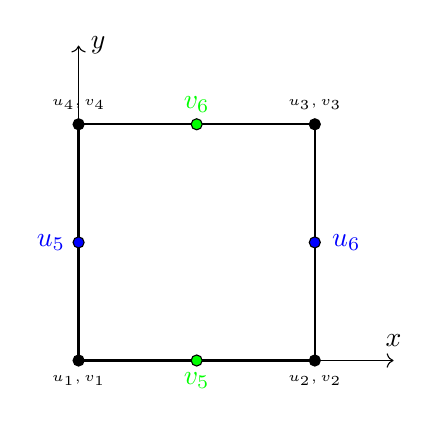
\begin{tikzpicture}
%\draw[fill=gray!23,gray!23](0,0) rectangle (6,5);
%\draw[step=0.5cm,gray,very thin] (0,0) grid (6,5); %background grid

\draw[thick] (1,.5) -- (4,.5) -- (4,3.5) -- (1,3.5) -- cycle; %front

\draw[thin,->] (4,0.5) -- (5,0.5); %x
\draw[thin,->] (1,3.5) -- (1,4.5); %y
\node[] at (5,0.75) {$x$};
\node[] at (1.25,4.5) {$y$};

\draw[black,fill=black] (1,.5)   circle (2pt);
\draw[black,fill=black] (4,.5)   circle (2pt);
\draw[black,fill=black] (4,3.5)   circle (2pt);
\draw[black,fill=black] (1,3.5)   circle (2pt);

\node[] at (1,0.25) {\tiny $u_1,v_1$};
\node[] at (4,0.25) {\tiny $u_2,v_2$};
\node[] at (4,3.75) {\tiny $u_3,v_3$};
\node[] at (1,3.75) {\tiny $u_4,v_4$};

\draw[black,fill=blue] (1,2) circle (2pt); 
\draw[black,fill=blue] (4,2) circle (2pt); 
\node[] at (0.65,2) {\color{blue} $u_5$};
\node[] at (4.4,2) {\color{blue} $u_{6}$};

\draw[black,fill=green] (2.5,0.5) circle (2pt); 
\draw[black,fill=green] (2.5,3.5) circle (2pt); 
\node[] at (2.5,0.25) {\color{green} $v_5$};
\node[] at (2.5,3.75) {\color{green} $v_{6}$};

\end{tikzpicture}\\
\end{center}


\noindent The approximation of the velocity components $u$ and $v$ inside the element is
\[
u^h(r,s) = a^u \; N_1(r,s) + b^u \;  N_2(r,s) + c^u \; N_3(r,s) +d^u \; N_4(r,s) 
+ d\; b_5^u(r,s) + e\; b_{6}^u(r,s)
\]
\[
v^h(r,s) = a^v \; N_1(r,s) + b^v \;  N_2(r,s) + c^v \; N_3(r,s) +d^v \; N_4(r,s) 
+ d^v b_5^v(r,s) + e^v b_{6}^v(r,s)
\]
where $N_{1,2,3,4}$ are the standard $Q_1$ basis functions in 2D and with 
\[
b_5^u(r,s) = \frac{1}{2}(1-r)(1-s^2)
\qquad
b_6^u(r,s) = \frac{1}{2}(1+r)(1-s^2)
\]
and
\[
b_5^v(r,s) = \frac{1}{2}(1-r^2)(1-s)
\qquad
b_6^v(r,s) = \frac{1}{2}(1-r^2)(1+s)
\]
In the end one arrives at

\begin{mdframed}[backgroundcolor=blue!5]
\begin{eqnarray}
{N}_1^u(r,s) &=&  N_1(r,s) - \frac{1}{2} b_5^u(r,s)\nn\\
{N}_2^u(r,s) &=&  N_2(r,s) - \frac{1}{2} b_6^u(r,s)\nn\\
{N}_3^u(r,s) &=&  N_3(r,s) - \frac{1}{2} b_6^u(r,s)\nn\\
{N}_4^u(r,s) &=&  N_4(r,s) - \frac{1}{2} b_5^u(r,s)\nn\\
{N}_5^u(r,s) &=&  b_5^u(r,s) \nn\\
{N}_6^u(r,s) &=&  b_6^u(r,s) \nn\\
\nn\\
{N}_1^v(r,s) &=&  N_1(r,s) - \frac{1}{2} b_5^v(r,s)\nn\\
{N}_2^v(r,s) &=&  N_2(r,s) - \frac{1}{2} b_5^v(r,s)\nn\\
{N}_3^v(r,s) &=&  N_3(r,s) - \frac{1}{2} b_6^v(r,s)\nn\\
{N}_4^v(r,s) &=&  N_4(r,s) - \frac{1}{2} b_6^v(r,s)\nn\\
{N}_5^v(r,s) &=&  b_5^v(r,s) \nn\\
{N}_6^v(r,s) &=&  b_6^v(r,s) 
\end{eqnarray}
\end{mdframed}

We can check for the zero-th order consistency: Let $u(r,s)=C$, then 
\begin{eqnarray}
u^h(r,s) 
= \sum_{i=1}^6 N_i^u(r,s) u_i 
= C \sum_{i=1}^6 N_i^u(r,s) 
= C \sum_{i=1}^4 N_i(r,s)  
= C
\end{eqnarray}



\newpage
%-----------------------------------------------------------------------------
\subsubsection{The DSSY element} \label{ss:dssy_2D}
This element is often reffered to as the 'DSSY' element becaus of the 
four authors of the original paper: Douglas, Santos, sheen and Ye (1999) \cite{doss99}.

The non-conforming finite element space i$Q_l$ is defined based on the 
reference square element on $[-1,1]^2$ :
\[
Q_l = \text{Span} \left\{ 1, r, s, \theta_l(r)-\theta_l(s)  \right\}
\qquad l=1,\; \text{or} \; 2
\]
with
\begin{eqnarray}
\theta_1(r)  &=& r^2-\frac53r^4  \nn\\
\theta_1'(r) &=& 2r-\frac{20}{3}r^3  \nn\\
\theta_2(r)  &=& r^2-\frac{25}{6} r^4 + \frac72 r^6 \\ 
\theta_2'(r) &=& 2r-\frac{50}{3} r^3 + 21 r^5
\end{eqnarray}
The dimension of $Q_l$ is four and the $\theta_l$ functions look like:
\begin{center}
\includegraphics[width=7cm]{images/dssy/theta1}
\includegraphics[width=7cm]{images/dssy/theta2}
\end{center}
We have:
\begin{itemize}
\item $\theta_1(r=-1)=\theta_1(r=+1)=-\frac23$, $\theta_1(r=0)=0$ 
\item $\theta_2(r=-1)=\theta_2(r=+1)=\frac13$, $\theta_2(r=0)=0$ 
\end{itemize}
The nodes are situated at the mid-edges of the quadrilateral:

\input{tikz_dssy2D}

The basis function corresponding to the node (1, 0) is given by
\begin{mdframed}[backgroundcolor=blue!5]
\begin{eqnarray}
N_1(r,s)^{(l)} &=& \frac{1}{4} - \frac{1}{2} r + \frac{\theta_l(r)-\theta_l(s)}{4 \theta_l(1)}  \nn\\
N_2(r,s)^{(l)} &=& \frac{1}{4} + \frac{1}{2} r + \frac{\theta_l(r)-\theta_l(s)}{4 \theta_l(1)}  \nn\\
N_3(r,s)^{(l)} &=& \frac{1}{4} - \frac{1}{2} s - \frac{\theta_l(r)-\theta_l(s)}{4 \theta_l(1)}  \nn\\
N_4(r,s)^{(l)} &=& \frac{1}{4} + \frac{1}{2} s - \frac{\theta_l(r)-\theta_l(s)}{4 \theta_l(1)}  
\end{eqnarray}
\end{mdframed}
We can easily verify that $\sum_i N_i(r,s,t)=1$ and that $N_i(\vec{r}_j)=\delta_{ij}$:
\begin{eqnarray}
N_1^{(l)}(r_1,s_1) 
&=& \frac{1}{4} -\frac{1}{2} (-1) + \frac{\theta_l(-1)-\theta_l(0)}{4 \theta_l(1)}  
= \frac{1}{4} +\frac{1}{2}  + \frac{\theta_l(-1)}{4 \theta_l(1)}  
= \frac{1}{4} +\frac{1}{2}  + \frac{1}{4}   = 1 \nn\\
N_1^{(l)}(r_2,s_2)
&=& \frac{1}{4} -\frac{1}{2} (+1) + \frac{\theta_l(+1)-\theta_l(0)}{4 \theta_l(1)}  
= \frac{1}{4} -\frac{1}{2} + \frac{\theta_l(+1)}{4 \theta_l(1)}  
= \frac{1}{4} -\frac{1}{2} + \frac{1}{4}   = 0 \nn\\
N_1^{(l)}(r_3,s_3)
&=& \frac{1}{4} -\frac{1}{2} (0) + \frac{\theta_l(0)-\theta_l(-1)}{4 \theta_l(1)}  
= \frac14 -\frac14  = 0 \nn\\
N_1^{(l)}(r_4,s_4)
&=& \frac{1}{4} -\frac{1}{2} (0) + \frac{\theta_l(0)-\theta_l(+1)}{4 \theta_l(1)}  
= \frac14 -\frac14  = 0 \nn\\
N_2^{(l)}(r_1,s_1) 
&=& \frac{1}{4} + \frac{1}{2} (-1) + \frac{\theta_l(-1)-\theta_l(0)}{4 \theta_l(1)}  
= \frac14 -\frac12 + \frac14 = 0 \nn\\
N_2^{(l)}(r_2,s_2)
&=& \frac{1}{4} + \frac{1}{2} (+1) + \frac{\theta_l(+1)-\theta_l(0)}{4 \theta_l(1)}  
= \frac14 + \frac12 + \frac14 =1 \nn\\
N_2^{(l)}(r_3,s_3)
&=& \frac{1}{4} + \frac{1}{2} (0) + \frac{\theta_l(0)-\theta_l(-1)}{4 \theta_l(1)}  
= \frac14 - \frac14 = 0 \nn\\
N_2^{(l)}(r_4,s_4)
&=& \frac{1}{4} + \frac{1}{2} (0) + \frac{\theta_l(0)-\theta_l(+1)}{4 \theta_l(1)}  
= \frac14 - \frac14 = 0 \nn\\
N_3^{(l)}(r_1,s_1)
&=& \frac{1}{4} - \frac{1}{2} (0) - \frac{\theta_l(-1)-\theta_l(0)}{4 \theta_l(1)} 
= \frac14 -\frac14 = 0\nn\\
N_3^{(l)}(r_2,s_2)
&=& \frac{1}{4} - \frac{1}{2} (0) - \frac{\theta_l(+1)-\theta_l(0)}{4 \theta_l(1)} 
= \frac14 -\frac14 = 0\nn\\
N_3^{(l)}(r_3,s_3)
&=& \frac{1}{4} - \frac{1}{2} (-1) - \frac{\theta_l(0)-\theta_l(-1)}{4 \theta_l(1)} 
= \frac14 +\frac12 + \frac14 = 1\nn\\
N_3^{(l)}(r_4,s_4)
&=& \frac{1}{4} - \frac{1}{2} (+1) - \frac{\theta_l(0)-\theta_l(+1)}{4 \theta_l(1)} 
= \frac14 -\frac12 + \frac14 = 0\nn\\
N_4^{(l)}(r_1,s_1)
&=& \frac{1}{4} + \frac{1}{2} (0) - \frac{\theta_l(-1)-\theta_l(0)}{4 \theta_l(1)}  
= \frac14 -\frac14 =0\nn\\
N_4^{(l)}(r_2,s_2)
&=& \frac{1}{4} + \frac{1}{2} (0) - \frac{\theta_l(+1)-\theta_l(0)}{4 \theta_l(1)}  
= \frac14 -\frac14 =0\nn\\
N_4^{(l)}(r_3,s_3)
&=& \frac{1}{4} + \frac{1}{2} (-1) - \frac{\theta_l(0)-\theta_l(-1)}{4 \theta_l(1)}  
= \frac14 -\frac12 +\frac14 = 0 \nn\\
N_4^{(l)}(r_4,s_4)
&=& \frac{1}{4} + \frac{1}{2} (1) - \frac{\theta_l(0)-\theta_l(1)}{4 \theta_l(1)}  
= \frac14 +\frac12 +\frac14 = 1 \nn
\end{eqnarray}

The basis functions can also be explicitely written for $\theta_1$ as in Cai \etal \cite{cady99}:
\begin{eqnarray}
N_1(r,s)^{(l)} 
&=& \frac{1}{4} - \frac{1}{2} r - \frac38 \left[\left( r^2-\frac53r^4 \right) - \left(s^2-\frac53s^4 \right) \right] \nn\\
N_2(r,s)^{(l)} 
&=& \frac{1}{4} + \frac{1}{2} r - \frac38 \left[\left( r^2-\frac53r^4 \right) - \left(s^2-\frac53s^4 \right) \right] \nn\\
N_3(r,s)^{(l)} 
&=& \frac{1}{4} - \frac{1}{2} s + \frac38 \left[\left( r^2-\frac53r^4 \right) - \left(s^2-\frac53s^4 \right) \right] \nn\\
N_4(r,s)^{(l)} 
&=& \frac{1}{4} + \frac{1}{2} s + \frac38 \left[\left( r^2-\frac53r^4 \right) - \left(s^2-\frac53s^4 \right) \right] 
\end{eqnarray}

The derivatives of the basis functions are as follows:
\begin{eqnarray}
\partial_r N_1(r,s)^{(l)} &=&  - \frac{1}{2}  + \frac{\theta_l'(r)}{4 \theta_l(1)}  \nn\\
\partial_r N_2(r,s)^{(l)} &=&  + \frac{1}{2}  + \frac{\theta_l'(r)}{4 \theta_l(1)}  \nn\\
\partial_r N_3(r,s)^{(l)} &=&  - \frac{\theta_l'(r)}{4 \theta_l(1)}  \nn\\
\partial_r N_4(r,s)^{(l)} &=&  - \frac{\theta_l'(r)}{4 \theta_l(1)}  
\end{eqnarray}

\begin{eqnarray}
\partial_s N_1(r,s)^{(l)} &=&   -\frac{\theta_l'(s)}{4 \theta_l(1)}  \nn\\
\partial_s N_2(r,s)^{(l)} &=&   -\frac{\theta_l'(s)}{4 \theta_l(1)}  \nn\\
\partial_s N_3(r,s)^{(l)} &=&   - \frac{1}{2} + \frac{\theta_l'(s)}{4 \theta_l(1)}  \nn\\
\partial_s N_4(r,s)^{(l)} &=&   + \frac{1}{2} + \frac{\theta_l'(s)}{4 \theta_l(1)}  
\end{eqnarray}





\Literature: 
Jeon \etal (2013) \cite{jens13},
Bangerth \etal (2017) \cite{baks17},
Sheen (2020) \cite{shee20}













 %-----------
\subsection{Elements and basis functions in 3D} 

%%%%%%%%%%%%%%%%%%%%%%%%%%%%%%%%%%%%%%%%%%%%%%%%%%%%%%%
\subsubsection{Linear basis functions in tetrahedra ($P_1$)}
\index{$P_1$}


\begin{verbatim}
(r_0,s_0) = (0,0,0)
(r_1,s_1) = (1,0,0)
(r_2,s_2) = (0,2,0)
(r_3,s_3) = (0,0,1)
\end{verbatim}

The basis polynomial is given by
\[
f(r,s,t)=c_0 + c_1 r + c_2 s + c_3 t
\]

\begin{eqnarray}
f_1 &=& f(r_1,s_1,t_1) = c_0 \\
f_2 &=& f(r_2,s_2,t_2) = c_0 + c_1\\
f_3 &=& f(r_3,s_3,t_3) = c_0 + c_2\\
f_4 &=& f(r_4,s_4,t_4) = c_0 + c_3
\end{eqnarray}

which yields:
\[
c_0=f_1
\quad
\quad
c_1=f_2-f_1
\quad
\quad
c_2=f_3-f_1
\quad
\quad
c_3=f_4-f_1
\]

\begin{eqnarray}
f(r,s,t) 
&=& c_0 + c_1 r + c_2 s + c_3 t \nonumber\\
&=& f_1 + (f_2-f_1) r + (f_3-f_1) s + (f_4-f_1) t \nonumber\\
&=& f_1 (1-r-s-t) + f_2 r + f_3 s + f_4 t \nonumber\\
&=& \sum_i N_i(r,s,t) f_i \nonumber
\end{eqnarray}

Finally,

\begin{mdframed}[backgroundcolor=blue!5]
\begin{eqnarray}
N_1(r,s,t) &=& 1-r-s-t \nonumber\\
N_2(r,s,t) &=& r \nonumber\\
N_3(r,s,t) &=& s \nonumber\\
N_4(r,s,t) &=& t \nonumber
\end{eqnarray}
\end{mdframed}









%%%%%%%%%%%%%%%%%%%%%%%%%%%%%%%%%%%%%%%%%%%%%%%%%%%%%%%
\subsubsection{Triquadratic basis functions in 3D ($Q_2$)}
\index{$Q_2$}

\begin{eqnarray}
N_{1}&=& 0.5r(r-1)  \;0.5s(s-1)\; 0.5t(t-1)  \nonumber\\
N_{2}&=& 0.5r(r+1)  \;0.5s(s-1)\; 0.5t(t-1)  \nonumber\\
N_{3}&=& 0.5r(r+1)  \;0.5s(s+1)\; 0.5t(t-1)  \nonumber\\
N_{4}&=& 0.5r(r-1)  \;0.5s(s+1)\; 0.5t(t-1)  \nonumber\\
N_{5}&=& 0.5r(r-1)  \;0.5s(s-1)\; 0.5t(t+1)  \nonumber\\
N_{6}&=& 0.5r(r+1)  \;0.5s(s-1)\; 0.5t(t+1)  \nonumber\\
N_{7}&=& 0.5r(r+1)  \;0.5s(s+1)\; 0.5t(t+1)  \nonumber\\
N_{8}&=& 0.5r(r-1)  \;0.5s(s+1)\; 0.5t(t+1)  \nonumber\\
N_{9}&=& (1.-r^2)   \;0.5s(s-1)\; 0.5t(t-1)  \nonumber\\
N_{10}&=& 0.5r(r+1) \;(1-s^2)  \; 0.5t(t-1)  \nonumber\\
N_{11}&=& (1.-r^2)  \;0.5s(s+1)\; 0.5t(t-1)  \nonumber\\
N_{12}&=& 0.5r(r-1) \;(1-s^2)  \; 0.5t(t-1)  \nonumber\\
N_{13}&=& (1.-r^2)  \;0.5s(s-1)\; 0.5t(t+1)  \nonumber\\
N_{14}&=& 0.5r(r+1) \;(1-s^2)  \; 0.5t(t+1)  \nonumber\\
N_{15}&=& (1.-r^2)  \;0.5s(s+1)\; 0.5t(t+1)  \nonumber\\
N_{16}&=& 0.5r(r-1) \;(1-s^2)  \; 0.5t(t+1)  \nonumber\\
N_{17}&=& 0.5r(r-1) \;0.5s(s-1)\; (1-t^2)  \nonumber\\
N_{18}&=& 0.5r(r+1) \;0.5s(s-1)\; (1-t^2)  \nonumber\\
N_{19}&=& 0.5r(r+1) \;0.5s(s+1)\; (1-t^2)  \nonumber\\
N_{20}&=& 0.5r(r-1) \;0.5s(s+1)\; (1-t^2)  \nonumber\\
N_{21}&=& (1-r^2)   \;(1-s^2)  \; 0.5t(t-1)  \nonumber\\
N_{22}&=& (1-r^2)   \;0.5s(s-1)\; (1-t^2)  \nonumber\\
N_{23}&=& 0.5r(r+1) \;(1-s^2)  \; (1-t^2)  \nonumber\\
N_{24}&=& (1-r^2)   \;0.5s(s+1)\; (1-t^2)  \nonumber\\
N_{25}&=& 0.5r(r-1) \;(1-s^2)  \; (1-t^2)  \nonumber\\
N_{26}&=& (1-r^2)   \;(1-s^2)  \; 0.5t(t+1)  \nonumber\\
N_{27}&=& (1-r^2)   \;(1-s^2)  \; (1-t^2)  \nonumber
\end{eqnarray}

 %-------------------------------
 %%%%%%%%%%%%%%%%%%%%%%%%%%%%%%%%%%%%%%%%%%%%%%%%%%%%%%%%%%%%%%%%%%%%%%%%%%%%%%%%

%%%%%%%%%%%%%%%%%%%%%%%%%%%%%%%%%%%%%%%%%%%%%%%%%%%%%%%%%%%%%%%%%%%%%%%%%%%%%%%%%%%%%%%%%%%%%%%%%%%
%\chapter{Solving the heat transport equation with linear Finite Elements \label{chapt5}} %%%%%%%%%
\begin{flushright} {\tiny {\color{gray} chapter5.tex}} \end{flushright}

\subsection{The diffusion equation in 1D} \label{sec:diff1D} 
Let us consider the following one-dimensional grid: 
\begin{center}
\includegraphics[width=10cm]{images/oneD/domain}
\end{center}
Its spans the domain $\Omega$ of length $L_x$. 
It is discretised by means of 
$nnx$ nodes and $nelx=nnx-1$ elements.
Zooming in on element which is bounded by two nodes $k$ and $k+1$,
its size (also sometimes called diameter) is $h_x=x_{k+1}-x_k$, 
and the temperature field we wish to compute is located on those 
nodes so that they are logically called $T_k$ and $T_{k+1}$:

\begin{center}
\includegraphics[width=8cm]{images/oneD/el1D}
\end{center}

We focus here on the 1D diffusion equation (no advection, no heat sources):
\begin{equation}
\rho C_p \frac{\partial T}{\partial t} 
= \frac{\partial }{\partial x} \left( k \frac{\partial T}{\partial x}  \right)
\end{equation}
This is the {\color{olive}strong form} of the ODE to solve.
I can multiply this equation by a function\footnote{This function should be well-behaved with special properties, but we here assume it is a polynomial function.} $f(x)$ and integrate it over $\Omega$:
\begin{equation}
\int_{\Omega} f(x)  \rho C_p\frac{\partial T}{\partial t} dx
=
\int_{\Omega} f(x) \frac{\partial }{\partial x} \left( k \frac{\partial T}{\partial x}  \right) dx
\end{equation}
Looking at the right hand side, it is of the form $\int u v'$ so that I naturally 
integrate it by parts:
\begin{equation}
\int_{\Omega} f(x) \frac{\partial }{\partial x} 
\left( k \frac{\partial T}{\partial x}  \right) dx
=
\left[
f(x) k \frac{\partial T}{\partial x}
\right]_{\partial \Omega}
-
\int_{\Omega} \frac{\partial f}{\partial x}  k \frac{\partial T}{\partial x}  dx
\end{equation}
Assuming there is no heat flux prescribed on the boundary (i.e. $q_x= - k \partial T/\partial x = 0$ ),
\todo[inline]{NOT happy with this statement!!} then:
\begin{equation}
\int_{\Omega} f(x) \frac{\partial }{\partial x} \left( k \frac{\partial T}{\partial x}  \right) dx
=
- \int_{\Omega} \frac{\partial f}{\partial x}  k \frac{\partial T}{\partial x}  dx
\end{equation}
We then obtain the {\color{olive}weak form} of the diffusion equation in 1D:
\begin{equation}
\boxed{
\int_{\Omega} f(x) \rho C_p \frac{\partial T}{\partial t} dx
+
\int_{\Omega} \frac{\partial f}{\partial x}  k \frac{\partial T}{\partial x}  dx = 0
}
\end{equation}
We then use the additive property of the integral 
$\int_\Omega \dots = \sum_{elts} \int_{\Omega_e} \dots$
so that 
\begin{equation}
\sum_{elts} \left(     
\underbrace{ \int_{\Omega_e} f(x) \rho C_p   \frac{\partial T}{\partial t} dx }_{{\Lambda}_f^e}
+
\underbrace{\int_{\Omega_e} \frac{\partial f}{\partial x}  k \frac{\partial T}{\partial x}  dx}_{{\Upsilon}_f^e}      \right) = 0  
\end{equation}

In order to compute these integrals (analytically or by means of a numerical quadrature), 
we will need to evaluate $T$ inside the element. However, inside the element, 
the temperature is not known: all we have is the temperature at the nodes. 
For $x\in [x_k,x_{k+1}]$ we need to come up with a way to compute the temperature at this location. 
It makes sense to think that $T(x)$ will then be a function of the temperature at the nodes, 
i.e. $T(x) = \alpha T_k + \beta T_{k+1}$ where $\alpha$ and $\beta$ are coefficients. 
One over-simplified approach would be to assign $T(x)=(T_k + T_{k+1})/2$ but this would make the
temperature discontinuous from element to element. 
The rather logical solution to this problem is a linear temperature field between $T_k$
and $T_{k+1}$: 

\begin{eqnarray}
T(x) 
%&=& N_{k}(x) T_k + N_{k+1}(x) T_{k+1}  \nn\\
&=& \underbrace{\frac{x_{k+1}-x}{h_x}}_{N_k^\theta(x)} T_k 
+ 
\underbrace{\frac{x-x_k}{h_x}}_{N_{k+1}^\theta(x)} T_{k+1} \nn
\end{eqnarray}
where $N_k^\theta(x)$ is the (temperature) shape function associated to node $k$ and 
$N_{k+1}^\theta(x)$ is the shape function associated to node $k+1$.

Rather reassuringly, we have:
\begin{itemize}
\item $x=x_k$ yields $T(x)=T_k$
\item $x=x_{k+1}$ yields $T(x)=T_{k+1}$
\item $x=(x_k+x_{k+1})/2$ yields $T(x)=(T_k+T_{k+1})/2$
\end{itemize}
In what follows we abbreviate $\partial T/\partial x$ by $\dot{T}$.
Let us compute ${\Lambda}_f^e$ and ${\Upsilon}_f^e$ separately.
\begin{eqnarray}
{\Lambda}_f^e 
&=&\int_{x_k}^{x_{k+1}} f(x) \rho C_p \dot T(x) dx \nn\\
&=& \int_{x_k}^{x_{k+1}} f(x) \rho C_p \;\;  [ N_{k}^\theta(x) \dot{T}_k + N_{k+1}^\theta(x) \dot{T}_{k+1} ] \;\; dx  \nn\\
&=& \int_{x_k}^{x_{k+1}} f(x) \rho C_p N_{k}^\theta(x) \dot{T}_k  dx  
+ \int_{x_k}^{x_{k+1}} f(x) \rho C_p N_{k+1}^\theta(x) \dot{T}_{k+1}   dx \nn\\
&=&  \left( \int_{x_k}^{x_{k+1}} f(x) \rho C_p  N_{k}^\theta(x) dx \right) \dot{T}_k  
+ \left( \int_{x_k}^{x_{k+1}} f(x) \rho C_p N_{k+1}^\theta(x) dx \right)  \dot{T}_{k+1}  \nn
\end{eqnarray}
Taking $f(x)=N_k^\theta(x)$ and omitting '$(x)$' in the rhs:
\[
{\Lambda}_{N_k^\theta}^e=
%\int_{x_k}^{x_{k+1}} {\color{blue}f}(x) \rho C_p \dot{\color{blue}T}(x) dx
\left( \int_{x_k}^{x_{k+1}} \rho C_p  N_k^\theta N_{k}^\theta dx \right) \dot{T}_k  
+ \left( \int_{x_k}^{x_{k+1}} \rho C_p N_k^\theta N_{k+1}^\theta dx \right)  \dot{T}_{k+1} 
\]
Taking $f(x)=N_{k+1}^\theta(x)$ and omitting '$(x)$' in the rhs:
\[
{\Lambda}_{N_{k+1}^\theta}^e
%\int_{x_k}^{x_{k+1}} {\color{blue}f}(x) \dot{\color{blue}T}(x) dx
=  \left( \int_{x_k}^{x_{k+1}} \rho C_p N_{k+1}^\theta N_{k}^\theta dx \right) \dot{T}_k  
+ \left( \int_{x_k}^{x_{k+1}}  \rho C_p  N_{k+1}^\theta N_{k+1}^\theta dx \right)  \dot{T}_{k+1} 
\]
We can rearrange these last two equations as follows:
\[
\left(
\begin{array}{c}
{\Lambda}_{N_k^\theta}^e  \\ \\ {\Lambda}_{N_{k+1}^\theta}^e
\end{array}
\right)
=
\left(
\begin{array}{cc}
\int_{x_k}^{x_{k+1}} N_k^\theta     \rho C_p N_{k}^\theta dx  &  \int_{x_k}^{x_{k+1}} N_k^\theta  \rho C_p N_{k+1}^\theta dx \\ \\
\int_{x_k}^{x_{k+1}} N_{k+1}^\theta \rho C_p N_{k}^\theta dx  &  \int_{x_k}^{x_{k+1}} N_{k+1}^\theta \rho C_p N_{k+1}^\theta dx 
\end{array}
\right)
\cdot
\left(
\begin{array}{c}
\dot{T}_k \\ \\
\dot{T}_{k+1}
\end{array}
\right)
\]
and we can take the integrals outside of the matrix:
\[
\left(
\begin{array}{c}
{\Lambda}_{N_k^\theta}^e \\ \\ {\Lambda}_{N_{k+1}^\theta}^e
\end{array}
\right)
=
\left[
\int_{x_k}^{x_{k+1}}
\rho C_p
\left(
\begin{array}{cc}
N_k^\theta N_{k}^\theta     &  N_k^\theta N_{k+1}^\theta  \\ \\
N_{k+1}^\theta N_{k}^\theta &  N_{k+1}^\theta N_{k+1}^\theta 
\end{array}
\right)
dx
\right]
\cdot
\left(
\begin{array}{c}
\dot{T}_k \\ \\ 
\dot{T}_{k+1}
\end{array}
\right)
\]
Finally, we can define the vectors 
\[
{\vec N}^T = 
\left(
\begin{array}{c}
N_k^\theta(x)  \\ \\  N_{k+1}^\theta (x)
\end{array}
\right)
\]
and 
\[
{\vec T}^e = 
\left(
\begin{array}{c}
T_k \\ \\ T_{k+1}
\end{array}
\right)
\quad
\quad
\quad
\quad
\quad
\dot{\vec T}^e = 
\left(
\begin{array}{c}
\dot{T}_k \\ \\ \dot{T}_{k+1}
\end{array}
\right)
\]
so that 
\[
\left(
\begin{array}{c}
{\Lambda}_{N_k^\theta}^e \\  \\ {\Lambda}_{N_{k+1}^\theta}^e
\end{array}
\right)
=
\left( \int_{x_k}^{x_{k+1}}   {\vec N}^T \rho C_p  {\vec N} dx  \right) \cdot \dot{\vec T}^e
\]

Back to the diffusion term:

\begin{eqnarray}
{\Upsilon}_f^e &=&
\int_{x_k}^{x^{k+1}} \frac{\partial f}{\partial x} k \frac{\partial T}{\partial x} dx \nn\\
&=&
\int_{x_k}^{x^{k+1}} \frac{\partial f}{\partial x} k \frac{\partial  (N_{k}^\theta(x) T_k + N_{k+1}^\theta(x) T_{k+1} ) }{\partial x} dx  \nn\\
%&=&
%\int_{x_k}^{x^{k+1}} \left( \frac{\partial {\color{blue}f}}{\partial x}  \frac{\partial  {\color{blue}N}_{k} } {\partial x}  T_k 
%+ \frac{\partial {\color{blue}f}}{\partial x}  \frac{\partial  {\color{blue}N}_{k+1} } {\partial x}  T_{k+1} \right)  dx \nn\\
&=&
\left( \int_{x_k}^{x^{k+1}} \frac{\partial f}{\partial x}  k \frac{\partial  N_{k}^\theta } {\partial x}  dx \right)  T_k 
+ \left( \int_{x_k}^{x^{k+1}} \frac{\partial f}{\partial x}  k \frac{\partial  N_{k+1}^\theta } {\partial x} dx \right) T_{k+1}  \nn
\end{eqnarray}
Taking $f(x)=N_k^\theta(x)$ 
\[
{\Upsilon}_{N_k^\theta}^e=
%\int_{x_k}^{x^{k+1}} \frac{\partial {\color{blue}f}}{\partial x} \frac{\partial {\color{blue}T}}{\partial x} dx
\left( \int_{x_k}^{x^{k+1}} k\frac{\partial N_k^\theta}{\partial x}  \frac{\partial  N_{k}^\theta } {\partial x}  dx \right)  T_k 
+ \left( \int_{x_k}^{x^{k+1}} k \frac{\partial N_k^\theta}{\partial x}  \frac{\partial  N_{k+1}^\theta } {\partial x} dx \right) T_{k+1}  \nn
\]
Taking $f(x)=N_{k+1}^\theta(x)$ 
\[
{\Upsilon}_{N_{k+1}^\theta}^e=
%\int_{x_k}^{x^{k+1}} \frac{\partial {\color{blue}f}}{\partial x} \frac{\partial {\color{blue}T}}{\partial x} dx
%=
\left( \int_{x_k}^{x^{k+1}} k\frac{\partial N_{k+1}^\theta}{\partial x}  \frac{\partial  N_{k}^\theta } {\partial x}  dx \right)  T_k 
+ \left( \int_{x_k}^{x^{k+1}}  k\frac{\partial N_{k+1}^\theta}{\partial x}  \frac{\partial  N_{k+1}^\theta } {\partial x} dx \right) T_{k+1}  \nn
\]


\[
\left(
\begin{array}{cc}
 {\Upsilon}_{N_k^\theta}^e \\ \\ {\Upsilon}_{N_{k+1}^\theta}^e
\end{array}
\right)
=
\left(
\begin{array}{cc}
\int_{x_k}^{x^{k+1}} \frac{\partial N_k^\theta}{\partial x} k \frac{\partial  N_{k}^\theta } {\partial x}  dx & 
\int_{x_k}^{x^{k+1}} \frac{\partial N_k^\theta}{\partial x} k \frac{\partial  N_{k+1}^\theta } {\partial x} dx 
\\ \\
\int_{x_k}^{x^{k+1}} \frac{\partial N_{k+1}^\theta}{\partial x} k \frac{\partial  N_{k}^\theta } {\partial x}  dx & 
\int_{x_k}^{x^{k+1}} \frac{\partial N_{k+1}^\theta}{\partial x} k \frac{\partial  N_{k+1}^\theta } {\partial x} dx 
\end{array}
\right)
\cdot
\left(
\begin{array}{c}
T_k \\ \\ T_{k+1}
\end{array}
\right)
\]

or,
\[
\left(
\begin{array}{cc}
 {\Upsilon}_{N_k^\theta}^e \\ \\ {\Upsilon}_{N_{k+1}^\theta}^e
\end{array}
\right)
=
\left[
\int_{x_k}^{x^{k+1}}
k
\left(
\begin{array}{cc}
\frac{\partial N_k^\theta}{\partial x}  \frac{\partial  N_{k}^\theta } {\partial x}   & 
\frac{\partial N_k^\theta}{\partial x}  \frac{\partial  N_{k+1}^\theta } {\partial x}  
\\ \\
\frac{\partial N_{k+1}^\theta}{\partial x}  \frac{\partial  N_{k}^\theta } {\partial x}   & 
\frac{\partial N_{k+1}^\theta}{\partial x}  \frac{\partial  N_{k+1}^\theta } {\partial x}  
\end{array}
\right)
dx
\right]
\cdot
\left(
\begin{array}{c}
T_k \\ \\ T_{k+1}
\end{array}
\right)
\]
Finally, we can define the vector 
\[
{\vec B}^T=
\left(
\begin{array}{cc}
 \frac{\partial N_k^\theta}{\partial x}   \\ \\
 \frac{\partial N_{k+1}^\theta}{\partial x}
\end{array}
\right)
\]
so that 
\[
\left(
\begin{array}{cc}
 {\Upsilon}_{N_k^\theta}^e \\ \\ {\Upsilon}_{N_{k+1}^\theta}^e
\end{array}
\right)
=
\left( \int_{x_k}^{x_{k+1}}   {\vec B}^T k {\vec B} dx  \right) \cdot {\vec T}^e
\]

The weak form discretised over 1 element becomes
\[
\underbrace{\left( \int_{x_k}^{x_{k+1}}   {\vec N}^T \rho C_p {\vec N} dx  \right) }_{\bm M^e} \cdot \dot{\vec T}^e
+
\underbrace{\left( \int_{x_k}^{x_{k+1}}   {\vec B}^T k {\vec B} dx  \right)}_{{\bm K}_d^e} \cdot {\vec T}^e
=0
\]
or,
\[
\boxed{
{\bm M}^e \cdot \dot{\vec T}^e + {\bm K}_d^e \cdot {\vec T}^e = 0
}
\]
or,
\[
\boxed{
{\bm M}^e \cdot \frac{\partial {\vec T}^e}{\partial t} + {\bm K}_d^e \cdot {\vec T}^e = 0
}
\]
${\bm M}^e$ is commonly called the mass matrix, or capacitance matrix \cite[p103]{reddybook2}.
\index{Mass matrix}\index{Capacitance matrix}

Using a backward first order in time discretisation for the time derivative:
\[
\dot{\vec T}= \frac{\partial {\vec T}}{\partial t} = \frac{{\vec T}^{new}-{\vec T}^{old}}{\delta t}
\]
we get
\[
{\bm M}^e \cdot \frac{{\vec T}^{new}-{\vec T}^{old}}{\delta t} + {\bm K}_d^e \cdot {\vec T}^{new} = 0
\]
or, 
\[
\boxed{
( {\bm M}^e +  {\bm K}_d^e  \delta t ) \cdot {\vec T}^{new} =  {\bm M}^e \cdot  {\vec T}^{old}
}
\]
with 
\[
{\bm M}^e=  \int_{x_k}^{x_{k+1}}   {\vec N}^T \rho C_p {\vec N} dx  
\quad\quad\quad
{\bm K}_d^e =
 \int_{x_k}^{x_{k+1}}   {\vec B}^T k {\vec B} dx 
\]

Let us compute ${\bm M}$ for an element:
\[
{\bm M}^e=  \int_{x_k}^{x_{k+1}}   {\vec N}^T \rho C_p {\vec N} dx  
\]
with 
\[
{\vec N}^T = 
\left(
\begin{array}{c}
N_k(x)  \\ \\  N_{k+1}(x)
\end{array}
\right)
=
\left(
\begin{array}{c}
\frac{x_{k+1}-x}{h_x}   \\ \\
\frac{x-x_k}{h_x} 
\end{array}
\right)
\]
Then 
\[
{\bm M}^e
=
\left(
\begin{array}{cc}
M_{11} & M_{12} \\
M_{21} & M_{22} 
\end{array}
\right)
=
\left(
\begin{array}{cc}
\int_{x_k}^{x_{k+1}} \rho C_p N_k^\theta N_{k}^\theta dx   &  \int_{x_k}^{x_{k+1}} \rho C_p N_k^\theta N_{k+1}^\theta dx \\ \\
\int_{x_k}^{x_{k+1}} \rho C_p N_{k+1}^\theta N_{k}^\theta dx  &  \int_{x_k}^{x_{k+1}} \rho C_p N_{k+1}^\theta N_{k+1}^\theta dx 
\end{array}
\right)
\]
I only need to compute 3 integrals since $M_{12}=M_{21}$.
Let us start with $M_{11}$:
\[
M_{11}=\int_{x_k}^{x_{k+1}} \rho C_p N_k^\theta(x) N_{k}^\theta(x) dx
=   
\int_{x_k}^{x_{k+1}} \rho C_p 
\frac{x_{k+1}-x}{h_x}  
\frac{x_{k+1}-x}{h_x}  
dx
\]
It is then customary to carry out the change of variable $x \rightarrow r$ where 
$r \in [-1:1]$ as shown hereunder:
\begin{center}
\includegraphics[width=8cm]{images/oneD/el1D_mapping}
\end{center}
The relationships between $x$ and $r$ are:
\[
r=\frac{2}{h_x}(x-x_k)-1
\quad\quad\quad
x=\frac{h_x}{2}(1+r)+x_k
\]

In what follows we assume for simplicity that $\rho$ and $C_p$ are constant within each element.
\[
M_{11}=
\rho C_p
\int_{\tiny x_k}^{x_{k+1}} 
\frac{x_{k+1}-x}{h_x}  
\frac{x_{k+1}-x}{h_x}  
dx
%=  \rho C_p \int_{-1}^{+1} \frac{1}{2}(1-r) \frac{1}{2}(1-r)  \frac{h_x}{2} dr  = \frac{h_x}{3} \rho C_p \nn
=  \frac{\rho C_p h_x}{8} \int_{-1}^{+1} (1-r) (1-r)  dr  = \frac{h_x}{3} \rho C_p
\]
Similarly we arrive at 
\begin{eqnarray}
M_{12}
%\rho C_p \int_{x_k}^{x_{k+1}}  {\color{blue}N}_k(x) {\color{blue}N}_{k+1}(x) dx
=\rho C_p 
\int_{x_k}^{x_{k+1}} 
\frac{x_{k+1}-x}{h_x}  
\frac{x-x_k}{h_x}  
dx
=
\frac{\rho C_p  h_x}{8} 
\int_{-1}^{+1} (1-r) (1+r)dr
= \frac{h_x}{6} \rho C_p \nn
\end{eqnarray}
and 
\[
M_{22}
%=\rho C_p \int_{x_k}^{x_{k+1}} {\color{blue}N}_{k+1}(x) {\color{blue}N}_{k+1}(x) dx
=
\rho C_p 
\int_{x_k}^{x_{k+1}} 
\frac{x-x_k}{h_x}  
\frac{x-x_k}{h_x}  
dx
=
\frac{\rho C_p  h_x}{8} 
\int_{-1}^{+1} (1+r) (1+r)dr
= \frac{h_x}{3} \rho C_p 
\]
Finally 
\[
\boxed{
{\bm M}^e= \frac{h_x}{3} \rho C_p  
\left(
\begin{array}{cc}
1  & 1/2 \\
1/2 & 1
\end{array}
\right)
}
\]

In the new coordinate system, the {\color{olive}shape functions} 
\[
N_k^\theta(x) = \frac{x_{k+1}-x}{h_x} 
\quad
\quad
\quad
N_{k+1}^\theta(x) = \frac{x-x_k}{h_x} 
\]
become 
\[
N_k^\theta(r) = \frac{1}{2} (1-r)
\quad
\quad
\quad
N_{k+1}^\theta(r) = \frac{1}{2} (1+r)
\]

Also, 
\[
\frac{\partial N_k^\theta}{\partial x} = - \frac{1}{h_x} 
\quad
\quad
\quad
\frac{\partial N_{k+1}^\theta}{\partial x} = \frac{1}{h_x} 
\]
so that 
\[
{\vec B}^T=
\left(
\begin{array}{cc}
 \frac{\partial N_k^\theta}{\partial x}   \\ \\
 \frac{\partial N_{k+1}^\theta}{\partial x}
\end{array}
\right)
=
\left(
\begin{array}{cc}
-\frac{1}{h_x} \\ \\
\frac{1}{h_x} 
\end{array}
\right)
\]


We here also assume that $k$ is constant within the element:
\[
{\bm K}_d =
\int_{x_k}^{x_{k+1}}   {\vec B}^T k {\vec B} dx 
= k \int_{x_k}^{x_{k+1}}   {\vec B}^T {\vec B} dx 
\]
simply becomes
\[
{\bm K}_d = k
 \int_{x_k}^{x_{k+1}} 
\frac{1}{h_x^2}
\left(
\begin{array}{cc}
1 & -1 \\ -1 & 1
\end{array}
\right)
dx
\]
and then
\[
\boxed{
{\bm K}_d =
\frac{k}{h_x}
\left(
\begin{array}{cc}
1 & -1 \\ -1 & 1
\end{array}
\right)
}
\]

Let us consider this very simple grid consisting of 4 elements/5 nodes:
\begin{center}
\includegraphics[width=10cm]{images/oneD/grid5}
\end{center}
For each element we have 
\[
\underbrace{( {\bm M}^e +  {\bm K}_d^e \; \delta t )}_{\bm A^{e}} \cdot {\vec T}^{new} =  \underbrace{{\bm M}^e \cdot  {\vec T}^{old} }_{\vec b^{e}}
\]
%or, 
%\[
%{\bm A}^{e}\cdot {\vec T}^{new} =  {\vec b}^{e}
%\]
We can write this equation very explictely for each element:
\begin{itemize}
\item element {\color{red}\tt 1} 
\[
{\bm A}^{\color{red} \tt 1}  \cdot 
\left(
\begin{array}{c}
T_1 \\ T_2
\end{array}
\right)
 =  {\vec b}^{\color{red} \tt 1}
\]
\[
\left\{ 
\begin{array}{l}
A_{11}^{{\color{red}\tt 1}} T_1 + A_{12}^{{\color{red}\tt 1}} T_2 = b^{{\color{red} \tt 1}}_x \\
A_{21}^{{\color{red}\tt 1}} T_1 + A_{22}^{{\color{red}\tt 1}} T_2 = b^{{\color{red} \tt 1}}_y
\end{array}
\right.
\]

\item element {\color{red}\tt 2} 
\[
{\bm A}^{\color{red} \tt 2}  \cdot 
\left(
\begin{array}{c}
T_2 \\ T_3
\end{array}
\right)
 =  {\vec b}^{\color{red} \tt 2}
\]
\[
\left\{ 
\begin{array}{l}
A_{11}^{{\color{red}\tt 2}} T_2 + A_{12}^{{\color{red}\tt 2}} T_3 = b^{{\color{red} \tt 2}}_1 \\
A_{21}^{{\color{red}\tt 2}} T_2 + A_{22}^{{\color{red}\tt 2}} T_3 = b^{{\color{red} \tt 2}}_2
\end{array}
\right.
\]


\item element {\color{red}\tt 3} 
\[
{\bm A}^{\color{red} \tt 3}  \cdot 
\left(
\begin{array}{c}
T_3 \\ T_4
\end{array}
\right)
 =  {\vec b}^{\color{red} \tt 3}
\]
\[
\left\{ 
\begin{array}{l}
A_{11}^{{\color{red}\tt 3}} T_3 + A_{12}^{{\color{red} \tt 3}} T_4 = b^{{\color{red} \tt 3}}_1 \\
A_{21}^{{\color{red}\tt 3}} T_3 + A_{22}^{{\color{red} \tt 3}} T_4 = b^{{\color{red} \tt 3}}_2
\end{array}
\right.
\]


\item element {\color{red}\tt 4} 
\[
{\bm A}^{\color{red} \tt 4}  \cdot 
\left(
\begin{array}{c}
T_4 \\ T_5
\end{array}
\right)
 =  {\vec b}^{\color{red} \tt 4}
\]
\[
\left\{ 
\begin{array}{l}
A_{11}^{{\color{red}\tt 4}} T_4 + A_{12}^{{\color{red}\tt 4}} T_5 = b^{{\color{red}\tt 4}}_1 \\
A_{21}^{{\color{red}\tt 4}} T_4 + A_{22}^{{\color{red}\tt 4}} T_5 = b^{{\color{red}\tt 4}}_2
\end{array}
\right.
\]
\end{itemize}

All equations can be cast into a single linear system: this is the {\color{olive} assembly} phase.
The process can also be visualised as shown hereunder. Because nodes 2,3,4 belong to two elements 
elemental contributions will be summed in the matrix and the rhs:
\begin{center}
\includegraphics[width=8.5cm]{images/oneD/assembly}
\end{center}
The assembled matrix and rhs are then:
\[
\left(
\begin{array}{ccccc}
A_{11}^{{\color{red}\tt 1}} &  A_{12}^{{\color{red}\tt 1}} &0&0&0 \\ \\ 
A_{21}^{{\color{red}\tt 1}} &  A_{22}^{{\color{red} \tt 1}} \!+\! A_{11}^{{\color{red}\tt 2}}  & A_{12}^{{\color{red}\tt 2}}   &0&0 \\ \\
0& A_{21}^{{\color{red}\tt 2}} & A_{22}^{{\color{red} \tt 2}} \! +\! A_{11}^{{\color{red}\tt 3}}  & A_{12}^{{\color{red}\tt 3}}   & 0\\ \\
0&0& A_{21}^{{\color{red}\tt 3}}   & A_{22}^{{\color{red}\tt 3}} \! +\! A_{11}^{{\color{red}\tt 4}}   & A_{12}^{{\color{red}\tt 4}}  \\ \\
0&0&0& A_{21}^{{\color{red}\tt 4}}   & A_{22}^{{\color{red}\tt 4}} 
\end{array}
\right)
\left(
\begin{array}{c}
T_1 \\\\ T_2 \\\\ T_3 \\\\ T_4 \\\\ T_5
\end{array}
\right)
=
\left(
\begin{array}{c}
b_{1}^{{\color{red}\tt 1}} \\ \\
b_{2}^{{\color{red}\tt 1}} + b_{1}^{{\color{red}\tt 2}}\\ \\
b_{2}^{{\color{red}\tt 2}} + b_{1}^{{\color{red}\tt 3}}\\ \\
b_{2}^{{\color{red}\tt 3}} + b_{1}^{{\color{red}\tt 4}}\\ \\
b_{2}^{{\color{red}\tt 4}} 
\end{array}
\right)
\]
Ultimately the assembled matrix system also takes the form
\[
\left(
\begin{array}{ccccc}
A_{11} & A_{12} & 0& 0& 0\\ \\
A_{21} & A_{22} & A_{23}& 0 & 0\\\\
0 & A_{32} & A_{33}&  A_{34}  & 0\\\\
0&0&   A_{43} & A_{44}&  A_{45} \\\\
0&0&0   & A_{54}&  A_{55} \\\\
\end{array}
\right)
\left(
\begin{array}{c}
T_1 \\\\ T_2 \\\\ T_3 \\\\ T_4 \\\\ T_5
\end{array}
\right)
=
\left(
\begin{array}{c}
b_1\\\\
b_2\\\\
b_3\\\\
b_4\\\\
b_5
\end{array}
\right)
\]
and we see that it is sparse. Its sparsity structure is easy to derive: each row corresponds to a dof, 
and since nodes 1 and 2 'see' each other (they belong to the same element) there will be non-zero entries
in the first and second column. 
Likewise, node 2 'sees' node 1 (in other words, there is an edge linking nodes 1 and 2), itself, 
and node 3, so that there are non-zero entries in the second row at columns 1, 2, and 3.

Before we solve the system, we need to take care of boundary conditions.
Let us assume that we wish to fix the temperature at node 2, or in other words 
we wish to set 
\[
T_2 = T^{bc}
\]
This equation can be cast as
\[
\left(
\begin{array}{ccccc}
 0 & 1 & 0 & 0 & 0
\end{array}
\right)
\left(
\begin{array}{c}
T_1 \\ T_2 \\ T_3 \\ T_4 \\ T_5
\end{array}
\right)
=
\left(
\begin{array}{c}
0 \\
T^{bc} \\
0 \\
0 \\
0
\end{array}
\right)
\]

This replaces the second line in the previous matrix equation:
\[
\left(
\begin{array}{ccccc}
A_{11} & A_{12} & 0& 0& 0\\ \\
0 & 1 & 0 & 0 & 0 \\ \\
0 & A_{32} & A_{33}&  A_{34} & 0 \\\\
0&0&   A_{43} & A_{44}&  A_{45} \\\\
0&0&0   & A_{54}&  A_{55} \\\\
\end{array}
\right)
\left(
\begin{array}{c}
T_1 \\\\ T_2 \\\\ T_3 \\\\ T_4 \\\\ T_5
\end{array}
\right)
=
\left(
\begin{array}{c}
b_{1} \\ \\
T^{bc} \\ \\
b_{3}\\\\
b_{4}\\\\
b_{5}
\end{array}
\right)
\]
That's it, we have a linear system of equations which can be solved!






 %----------------------
\subsection{The advection-diffusion equation in 1D} \label{sec:advec-diff1D}\index{Advection-Diffusion}

We start with the 1D advection-diffusion equation
\begin{equation}
\rho c_p \left( \frac{\partial T}{\partial t} 
+ u \frac{\partial T}{\partial x}
\right)
= \frac{\partial }{\partial x} \left( k \frac{\partial T}{\partial x}  \right)
+H
\end{equation}
This is the {\color{olive}strong form} of the ODE to solve.
As in the previous section, I multiply this equation by a function $f(x)$ and integrate it over 
the domain $\Omega$:
\[
\int_{\Omega} f(x)  \rho c_p\frac{\partial T}{\partial t} dx
+
\int_{\Omega} f(x)  \rho c_p u \frac{\partial T}{\partial x} dx
\!=\!
\int_{\Omega} f(x) \frac{\partial }{\partial x}\! \left(\! k\! \frac{\partial T}{\partial x}\!  \right)\! dx
+
\int_{\Omega} f(x) H dx 
\]
As in the previous section I integrate the r.h.s. by parts:
\[
\int_{\Omega} f(x) \frac{\partial }{\partial x} \left( k \frac{\partial T}{\partial x}  \right) dx
=
\left[
f(x) k \frac{\partial T}{\partial x}
\right]_{\partial \Omega}
-
\int_{\Omega} \frac{\partial f}{\partial x}  k \frac{\partial T}{\partial x}  dx
\]
Disregarding the boundary term for now, 
we then obtain the {\color{olive}weak form} of the diffusion equation in 1D:
\[
\boxed{
\int_{\Omega} f(x) \rho c_p \frac{\partial T}{\partial t} dx
+
\int_{\Omega} f(x)  \rho c_p u \frac{\partial T}{\partial x} dx
+
\int_{\Omega} \frac{\partial f}{\partial x}  k \frac{\partial T}{\partial x}  dx = 
\int_{\Omega} f(x) H dx 
}
\]

We then use the additive property of the integral $\int_\Omega \dots = \sum_{elts} \int_{\Omega_e} \dots$
\[
\sum_{elts} \left(     
\underbrace{ \int_{\Omega_e} f(x) \rho c_p   \frac{\partial T}{\partial t} dx }_{{\Lambda}_f^e}
+
\underbrace{  \int_{\Omega_e} f(x)  \rho c_p u \frac{\partial T}{\partial x} dx  }_{{\Sigma}_f^e}
+
\underbrace{\int_{\Omega_e} \frac{\partial f}{\partial x}  k \frac{\partial T}{\partial x}  dx}_{{\Upsilon}_f^e}    
- 
\underbrace{\int_{\Omega_e} f(x) H dx }_{{\Omega}_f^e}
  \right) = 0  
\]

In the element, we have seen that the temperature can be written:

\[
T(x) 
= N^\theta_{k}(x) T_k + N^\theta_{k+1}(x) T_{k+1}  
\]
In the previous presentation we have computed  ${\Lambda}_f^e$ and ${\Upsilon}_f^e$.
Let us now turn to ${\Sigma}_f^e$ and ${\Omega}_f^e$.

\begin{eqnarray}
{\Sigma}_f^e 
&=&\int_{x_k}^{x_{k+1}} f(x) \rho c_p u\frac{\partial T}{\partial x} dx \nn\\
&=&\int_{x_k}^{x_{k+1}} f(x) \rho c_p u\frac{\partial [ N_{k}(x) {T}_k + N_{k+1}(x) {T}_{k+1} ] }{\partial x} dx \nn\\
&=&\int_{x_k}^{x_{k+1}} f(x) \rho c_p u\frac{\partial  N_{k} }{\partial x} T_k dx 
+  \int_{x_k}^{x_{k+1}} f(x) \rho c_p u\frac{\partial  N_{k+1} }{\partial x} T_{k+1} dx \nn\\
&=& \left(  \int_{x_k}^{x_{k+1}} f(x) \rho c_p u\frac{\partial  N_{k} }{\partial x} dx \right) T_k 
+ \left( \int_{x_k}^{x_{k+1}} f(x) \rho c_p u\frac{\partial  N_{k+1} }{\partial x} dx \right)T_{k+1}  \nn
%&=&  \int_{x_k}^{x_{k+1}} {\color{blue}f}(x) \rho c_p \;\;  [ {\color{blue}N}_{k}(x) \dot{T}_k + {\color{blue}N}_{k+1}(x) \dot{T}_{k+1} ] \;\; dx  \nn\\
%&=&  \int_{x_k}^{x_{k+1}} {\color{blue}f}(x) \rho c_p {\color{blue}N}_{k}(x) \dot{T}_k  dx  + \int_{x_k}^{x_{k+1}} {\color{blue}f}(x) \rho c_p {\color{blue}N}_{k+1}(x) \dot{T}_{k+1}   dx \nn\\
%&=&  \left( \int_{x_k}^{x_{k+1}} {\color{blue}f}(x) \rho c_p  {\color{blue}N}_{k}(x) dx \right) \dot{T}_k  
%+ \left( \int_{x_k}^{x_{k+1}} {\color{blue}f}(x) \rho c_p {\color{blue}N}_{k+1}(x) dx \right)  \dot{T}_{k+1}  \nn
\end{eqnarray}

Taking $f(x)=N_k(x)$ and omitting '$(x)$' in the rhs:
\[
{\Sigma}_{N_k}^e=
\left( \int_{x_k}^{x_{k+1}} \rho c_p u N_k \frac{\partial  N_{k} }{\partial x} dx \right) T_k 
+ 
\left( \int_{x_k}^{x_{k+1}} \rho c_p u N_k \frac{\partial  N_{k+1} }{\partial x} dx \right)T_{k+1}  \nn
\]
Taking $f(x)=N_{k+1}(x)$ and omitting '$(x)$' in the rhs:
\[
{\Sigma}_{N_{k+1}}^e=
\left( \int_{x_k}^{x_{k+1}} \rho c_p u N_{k+1} \frac{\partial  N_{k} }{\partial x} dx \right) T_k + 
\left( \int_{x_k}^{x_{k+1}} \rho c_p u N_{k+1} \frac{\partial  N_{k+1} }{\partial x} dx \right)T_{k+1}  \nn
\]



\[
\left(
\begin{array}{c}
{\Sigma}_{N_k}  \\ \\ {\Sigma}_{N_{k+1}}
\end{array}
\right)
\!=\!
\left(
\begin{array}{cc}
\int_{x_k}^{x_{k+1}} \rho c_p u N_k \frac{\partial  N_{k} }{\partial x} dx  & 
\int_{x_k}^{x_{k+1}} \rho c_p u N_k \frac{\partial  N_{k+1} }{\partial x} dx \\ \\
\int_{x_k}^{x_{k+1}} \rho c_p u N_{k+1} \frac{\partial  N_{k} }{\partial x} dx  & 
\int_{x_k}^{x_{k+1}} \rho c_p u N_{k+1} \frac{\partial  N_{k+1} }{\partial x} dx 
\end{array}
\right)
\!\cdot\!
\left(
\begin{array}{c}
{T}_k \\ \\
{T}_{k+1}
\end{array}
\right)
\]
or,
\[
\left(
\begin{array}{c}
{\Sigma}_{N_k} \\ \\ {\Sigma}_{N_{k+1}}
\end{array}
\right)
\!=\!
\left[
\int_{x_k}^{x_{k+1}}
\rho c_p u
\left(
\begin{array}{cc}
N_k \frac{\partial     N_{k} }{\partial x}   & 
N_k \frac{\partial     N_{k+1} }{\partial x}  \\ \\
N_{k+1} \frac{\partial N_{k} }{\partial x}   & 
N_{k+1} \frac{\partial N_{k+1} }{\partial x} 
\end{array}
\right)
dx
\right]
\cdot
\left(
\begin{array}{c}
{T}_k \\ \\ 
{T}_{k+1}
\end{array}
\right)
\]

Finally, we have already defined the vectors 
\[
{\vec N}^T = 
\left(
\begin{array}{c}
N_k(x)  \\ \\  N_{k+1} (x)
\end{array}
\right)
\quad\quad
{\vec B}^T=
\left(
\begin{array}{cc}
 \frac{\partial N_k}{\partial x}   \\ \\
 \frac{\partial N_{k+1}}{\partial x}
\end{array}
\right)
\quad
\quad
{\vec T}^e = 
\left(
\begin{array}{c}
T_k \\ \\ T_{k+1}
\end{array}
\right)
\]
so that 
\[
\left(
\begin{array}{c}
{\Sigma}_{N_k} \\  \\ {\Sigma}_{N_{k+1}}
\end{array}
\right)
=
\left( \int_{x_k}^{x_{k+1}}   {\vec N}^T \rho c_p u {\vec B} dx  \right) \cdot {\vec T}^e
= {\bm K}_a \cdot \vec T^e
\]
One can easily show that 
\[
{\bm K}_a^e=
\rho c_p u
\left(
\begin{array}{cc}
-1/2 & 1/2 \\ \\
-1/2 & 1/2 
\end{array}
\right)
\]
Note that the matrix ${\bm K}_a^e$ is {\sl not} symmetric. 

Let us now look at the source term:
\begin{eqnarray}
{\Omega}_f^e &=&
\int_{x_k}^{x^{k+1}} f(x) H(x) dx \nn
\end{eqnarray}
Taking $f(x)=N_k(x)$ 
\[
{\Omega}_{N_k}=
\int_{x_k}^{x^{k+1}} N_k(x) H(x) dx \nn
\]
Taking $f(x)=N_{k+1}(x)$ 
\[
{\Omega}_{N_{k+1}}=
\int_{x_k}^{x^{k+1}} N_{k+1}(x) H(x) dx \nn
\]
We can rearrange both equations as follows:
\[
\left(
\begin{array}{cc}
 {\Omega}_{N_k} \\ \\ {\Omega}_{N_{k+1}}
\end{array}
\right)
=
\left(
\begin{array}{cc}
\int_{x_k}^{x^{k+1}} N_k(x) H(x) dx \nn \\ \\ 
\int_{x_k}^{x^{k+1}} N_{k+1}(x) H(x) dx \nn
\end{array}
\right)
\]
or,
\[
\left(
\begin{array}{cc}
 {\Omega}_{N_k} \\ \\ {\Omega}_{N_{k+1}}
\end{array}
\right)
=
\left[
\int_{x_k}^{x^{k+1}}
\left(
\begin{array}{cc}
N_k(x)  H(x)  \nn \\ \\ 
N_{k+1}(x) H(x)  \nn
\end{array}
\right)
dx
\right]
\]
so that 
\[
\left(
\begin{array}{cc}
 {\Omega}_{N_k} \\ \\ {\Omega}_{N_{k+1}}
\end{array}
\right)
=
\left(
\int_{x_k}^{x^{k+1}}
{\vec N}^T H(x) dx
\right)
\]

The weak form discretised over 1 element becomes
\begin{eqnarray}
&&\underbrace{\left( \int_{x_k}^{x_{k+1}}   {\vec N}^T \rho c_p {\bm N} dx  \right) }_{\bm M^e} \cdot \dot{\vec T}^e
+
\underbrace{\left( \int_{x_k}^{x_{k+1}}   {\vec N}^T \rho c_p u {\bm B} dx  \right)}_{{\bm K}_a^e} \cdot {\vec T}^e 
 +
\underbrace{\left( \int_{x_k}^{x_{k+1}}   {\vec B}^T k {\bm B} dx  \right)}_{{\bm K}_d^e} \cdot {\vec T}^e 
=
\underbrace{\left( \int_{x_k}^{x_{k+1}}   {\vec N}^T H(x) dx \right)}_{{\vec F}^e} \nn 
\end{eqnarray}
or,
\[
\boxed{
{\bm M}^e \cdot \dot{\vec T}^e + ({\bm K}_d^e + {\bm K}_a^e)\cdot {\vec T}^e = {\vec F}^e
}
\]
or,
\[
\boxed{
{\bm M}^e \cdot \frac{\partial {\vec T}^e}{\partial t} + ({\bm K}_a^e + {\bm K}_d^e) \cdot {\vec T}^e = {\vec F}^e
}
\]











 %---
\subsection{The advection-diffusion equation in 2D} \label{ss:hte_fem}We start from the 'bare-bones' heat transport equation (source terms are omitted): 
\begin{equation}
\rho C_p \left( \frac{\partial T}{\partial t} + {\vec \upnu}\cdot {\vec\nabla T} \right)
= {\vec \nabla} \cdot k \vec\nabla T 
\end{equation}
In what follows we assume that the velocity vield $\vec \upnu$ is known so that temperature is the 
only unknwon.
Let $N^\uptheta$ be the temperature basis functions so that the temperature inside an element is 
given by\footnote{the $\uptheta$ superscript has been chosen to denote temperature so as to avoid confusion
with the transpose operator}:
\begin{equation}
T^h({\vec r}) = \sum_{i=1}^{m_T} N^\uptheta ({\vec r}) T_i = \vec N^\uptheta \cdot \vec T
\end{equation}
where $\vec T$ is a vector of length $m_T$
The weak form is then 
\begin{equation}
\int_\Omega N^\uptheta_i \left[ 
\rho C_p \left( \frac{\partial T}{\partial t} + {\vec \upnu}\cdot {\vec\nabla T} \right) \right] d\Omega
= \int_\Omega  N^\uptheta_i {\vec \nabla} \cdot k \vec\nabla T  d\Omega
\end{equation}

\[
\underbrace{\int_\Omega N^\uptheta_i  \rho C_p \frac{\partial T}{\partial t} d\Omega}_{I}
+ \underbrace{\int_\Omega N^\uptheta_i  \rho C_p  {\vec \upnu}\cdot {\vec\nabla T}   d\Omega}_{II}
= \underbrace{\int_\Omega  N^\uptheta_i {\vec \nabla} \cdot k \vec\nabla T d\Omega}_{III}
\quad\quad
i=1,m_T
\]

Looking at the first term:
\begin{eqnarray}
\int_\Omega N^\uptheta_i  \rho C_p \frac{\partial T}{\partial t} d\Omega
&=&  \int_\Omega N^\uptheta_i  \rho C_p \vec N^\uptheta \cdot \dot{\vec T}  d\Omega \\
\end{eqnarray}
so that when we assemble all contributions for $i=1,m_T$ we get:
\[
I 
= \int_\Omega \vec N^\uptheta  \rho C_p \vec N^\uptheta \cdot \dot{\vec T}  d\Omega
= \left( \int_\Omega \rho C_p  \vec N^\uptheta  \vec N^\uptheta  d\Omega \right) \cdot \dot{\vec T}
= {\bm M}^T \cdot \dot{\vec T}
 \]
where ${\bm M}^T$ is the mass matrix of the system of size $(m_T \times m_T)$ with 
\[
M_{ij}^T = \int_\Omega \rho C_p N_i^\uptheta N_j^\uptheta d\Omega
\]
Turning now to the second term:
\begin{eqnarray}
\int_\Omega N^\uptheta_i  \rho C_p  {\vec \upnu}\cdot {\vec\nabla T}   d\Omega
&=& \int_\Omega N^\uptheta_i  \rho C_p (u \frac{\partial T}{\partial x} +  v \frac{\partial T}{\partial y} ) d\Omega \\
&=& \int_\Omega N^\uptheta_i  \rho C_p (u \frac{\partial \vec N^\uptheta}{\partial x} +  v \frac{\partial \vec N^\uptheta}{\partial y} ) \cdot \vec T d\Omega \\
\end{eqnarray}
so that when we assemble all contributions for $i=1,m_T$ we get:
\[
II = \left(\int_\Omega \rho C_p \vec N^\uptheta (u \frac{\partial \vec N^\uptheta}{\partial x} +  v \frac{\partial \vec N^\uptheta}{\partial y} ) d\Omega \right)  \cdot \vec T = {\bm K}_a \cdot \vec T
\]
where ${\bm K}_a$ is the advection term matrix of size $(m_T \times m_T)$ with
\[
(K_a)_{ij} = \int_\Omega \rho C_p N_i^\uptheta 
\left(u \frac{\partial N_j^\uptheta}{\partial x} +  v \frac{\partial N_j^\uptheta}{\partial y} \right) d\Omega 
\]
Now looking at the third term, we carry out an integration by part and neglect the surface term for now, so that 
\begin{eqnarray}
\int_\Omega  N^\uptheta_i {\vec \nabla} \cdot k \vec\nabla T d\Omega
&=& - \int_\Omega  k \vec \nabla N^\uptheta_i \cdot \vec\nabla T d\Omega \\
&=& - \int_\Omega  k \vec \nabla N^\uptheta_i \cdot \vec\nabla (\vec N^\uptheta \cdot \vec T) d\Omega \\
\end{eqnarray}
with 
\[
\vec \nabla \vec N^\uptheta = 
\left(
\begin{array}{cccc}
\partial_x N_1^\uptheta & 
\partial_x N_2^\uptheta & \dots &
\partial_x N_{m_T}^\uptheta \\ \\
\partial_y N_1^\uptheta & 
\partial_y N_2^\uptheta & \dots &
\partial_y N_{m_T}^\uptheta 
\end{array}
\right)
\]
so that finally:
\[
III = - \left( \int_\Omega k (\vec \nabla \vec N^\uptheta)^T \cdot \vec \nabla \vec N^\uptheta d\Omega \right) \cdot \vec T
= - {\bm K}_d \cdot \vec T
\]
where ${\bm K}_d$ is the diffusion term matrix:
\[
{\bm K}_d = \int_\Omega  k (\vec \nabla \vec N^\uptheta)^T \cdot \vec \nabla \vec N^\uptheta d\Omega 
\]
 Ultimately terms $I,II,III$ together yield:
\[
\boxed{
{\bm M}^\uptheta \cdot \dot{\vec T} + ({\bm K}_a + {\bm K}_d) \cdot \vec T = \vec 0
}
\]
What now remains to be done is to address the time derivative on the temperature vector. 
The most simple approach would be to use an explicit Euler one, i.e.:
\[
\frac{\partial \vec T}{\partial t} = \frac{\vec T^{(k)} - \vec T^{(k-1)}}{\delta t}
\]
where $\vec T^{(k)}$ is the temperature field at time step $k$ and $\delta t$ is the time interval 
between two consecutive time steps.
In this case the discretised heat transport equation is:
\[
\boxed{
\left( {\bm M}^\uptheta  + ({\bm K}_a + {\bm K}_d) \delta t \right) \cdot \vec T^{(k)} =  {\bm M}^\uptheta \cdot \vec T^{(k-1)}
}
\]
\todo[inline]{add source term!!}




Let us then write this equation at times $t$ and $t+\delta t$ :
\begin{eqnarray}
{\bm M}^\uptheta(t) \cdot \dot{\vec T}(t) + {\bm K}(t) \cdot \vec T(t) &=& \vec F(t)  \label{htefem3} \\ 
{\bm M}^\uptheta(t+\delta t) \cdot \dot{\vec T}(t+\delta t) + {\bm K}(t+\delta t)\cdot {\vec T}(t+\delta t) &=& {\vec F}(t+\delta t) \label{htefem4} 
\end{eqnarray}
The time derivative of temperature can be written as follows:
\[
\frac{\vec T(t+\delta t)-\vec T(t) }{\delta t} = \alpha \dot{\vec T}(t+\delta t) + (1-\alpha) \dot{\vec T}(t)
\]
If $\alpha=0$ then this is a fully implicit scheme, if $\alpha=1$ this is a fully explicit scheme. 
If $\alpha=1/2$ this is a second order accurate, mid-point implicit scheme 
One can multiply Eq. (\ref{htefem3}) by $1-\alpha$ and Eq. (\ref{htefem4}) by $\alpha$ and sum them :
\begin{eqnarray}
(1-\alpha) {\bm M}^\uptheta(t) \cdot \dot{\vec T}(t) + (1-\alpha){\bm K}(t)\cdot {\vec T}(t)
&=& (1-\alpha){\vec F}(t)  \nn\\
+ \alpha  {\bm M}(t+\delta t) \cdot \dot{\vec T}(t+\delta t) 
+ \alpha {\bm K}(t+\delta t)\cdot {\vec T}(t+\delta t) && +  \alpha {\vec F}(t+\delta t) \nn 
\end{eqnarray}
Assuming ${\bm M}^\uptheta(t)\approx {\bm M}^\uptheta(t+\delta t)$, ${\bm K}(t+\delta t)={\bm K}(t)$  
and ${\vec F}(t)\approx {\vec F}(t+\delta t)$, then 
\begin{eqnarray}
{\bm M}(t) \cdot \frac{\vec T(t+\delta t)-\vec T(t) }{\delta t} 
+ (1-\alpha){\bm K}(t)\cdot {\vec T}(t)   
+ \alpha {\bm K}(t)\cdot {\vec T}(t+\delta t) 
&=& {\vec F}(t)  \nn
\end{eqnarray}
and finally
\[
\left[ {\bm M}^\uptheta(t) + \alpha {\bm K}(t) \; \delta t \right] \cdot  {\vec T}(t+\delta t)
= \left[ {\bm M}^\uptheta(t) - (1-\alpha) {\bm K}(t) \; \delta t \right] \cdot  {\vec T}(t) + {\vec F}(t) \; \delta t
\]
or, 
\[
{\bm A}\cdot {\vec T} = {\vec b}
\]
with 
\begin{eqnarray}
{\bm A} &=& {\bm M}^\uptheta(t) + \alpha {\bm K}(t) \; \delta t  \nn\\
{\vec b} &=& \left[ {\bm M}^\uptheta(t) - (1-\alpha) {\bm K}(t) \; \delta t \right] \cdot  {\vec T}(t) + {\vec F}(t) \; \delta t \nn
\end{eqnarray}


\todo[inline]{there's got to be a prettier way to arrive at this ...}

 %------------
\subsection{Another approach to solving the advection diffusion}\label{ss:hte_diff} 
As we have seen above, one usually solves the heat transport equation (i.e. 
an advection-diffusion equation) in this form (source terms are neglected):
\begin{equation}
\rho C_p \left( \frac{\partial T}{\partial t} + {\vec \upnu}\cdot {\vec\nabla T} \right)
= {\vec \nabla} \cdot k \vec\nabla T 
\end{equation}
As we have seen in Section~\ref{ss:hte}, the diffusion term is actually the divergence of the heat flux
$\vec{q}=-k \vec \nabla T$. We could then choose to keep the heat flux as an unknown and 
solve a coupled system of equations instead:
\begin{eqnarray}
\rho C_p \left( \frac{\partial T}{\partial t} + {\vec \upnu}\cdot {\vec\nabla T} \right)
&=& - {\vec \nabla} \cdot \vec{q} \nn\\ 
\vec{q} &=& - k \vec \nabla T \nn
\end{eqnarray}
or, 
\begin{eqnarray}
\rho C_p \left( \frac{\partial T}{\partial t} + {\vec \upnu}\cdot {\vec\nabla T} \right)
+ {\vec \nabla} \cdot \vec{q} &=& \vec{0} \label{eq:htediff1}\\ 
\vec{q} + k \vec \nabla T &=& \vec{0} \label{eq:htediff2}
\end{eqnarray}
We have seen that the two left hand side terms of the first equation become 
${\bm M}^\uptheta \cdot \dot{\vec{T}}$ and ${\bm K}_a \cdot \vec{T}$.
Let $N^\uptheta$ be the temperature basis functions so that the temperature inside an element is 
given by
\begin{equation}
T^h({\vec r}) = \sum_{i=1}^{m_T} N^\uptheta_i ({\vec r}) T_i = \vec N^\uptheta \cdot \vec T
\end{equation}
where $\vec T$ is a vector of length $m_T$.
Let $N^q$ be the heat flux basis functions, and let us define (in 2D) $\vec{q}=(\qx,\qy)$ so that 
\begin{eqnarray}
\qx^h({\vec r}) &=& \sum_{i=1}^{m_q} N^q_i ({\vec r}) \qx_i = \vec{N}^q \cdot \vec{\qx} \\
\qy^h({\vec r}) &=& \sum_{i=1}^{m_q} N^q_i ({\vec r}) \qy_i = \vec{N}^q \cdot \vec{\qy} 
\end{eqnarray}
where $\vec{N}^q$, $\vec{\qx}$ and $\vec{\qy}$ are vectors of length $m_q$.
The weak form of the third term of Eq.~(\ref{eq:htediff1}) is then
\begin{eqnarray}
\int_\Omega N_i^\theta  \nabla \cdot \vec{q} \;  d\Omega
&=& -\int_\Omega N_i^\theta  
\left(  \frac{\partial }{\partial x}\qx + \frac{\partial }{\partial y}\qy \right) d\Omega \nn\\
&=& \int_\Omega N_i^\theta  \left(  \frac{\partial \vec{N}^q}{\partial x}\cdot \vec{\qx}
+  \frac{\partial \vec{N}^q}{\partial y}\cdot \vec{\qy} \right) d\Omega \nn\\
&=& \int_\Omega N_i^\theta  \frac{\partial \vec{N}^q}{\partial x}\cdot  \vec{\qx} \;  d\Omega + 
\int_\Omega  N_i^\uptheta \frac{\partial \vec{N}^q}{\partial y} \cdot \vec{\qy} \;  d\Omega \nn
\end{eqnarray}
Writing this last equation for $i=1,...m_T$ yields
\[
\underbrace{\left( \int_\Omega \vec{N}^\theta  \frac{\partial \vec{N}^q}{\partial x} \; d\Omega \right)}_{{\bm H}_x} \cdot\vec{\qx}+ 
\underbrace{\left( \int_\Omega  \vec{N}^\uptheta \frac{\partial \vec{N}^q}{\partial y}  \;  d\Omega\right)}_{{\bm H}_y} \cdot \vec{\qy}
\]
In the end, we obtain:
\begin{equation}
{\bm M}^\uptheta \cdot \dot{\vec{T}} + {\bm K}_a \cdot \vec{T} 
+ {\bm H}_x \cdot \vec{\qx}
+ {\bm H}_y \cdot \vec{\qy}
=\vec{0} \label{eq:htediff3}
\end{equation}
Turning now to Eq.~(\ref{eq:htediff2}), its weak form is
\[
\int_\Omega N_i^q \left( \vec{q} + k \vec \nabla T \right) d\Omega = \vec{0}
\]
and we can decompose it in its $x$ and $y$ components:
%\begin{eqnarray}
%\int_\Omega N_i^q \left( \qx + k  \frac{\partial T}{\partial x} \right) d\Omega &=& 0 \nn\\
%\int_\Omega N_i^q \left( \qy + k  \frac{\partial T}{\partial y} \right) d\Omega &=& 0 \nn
%\end{eqnarray}
%We process these further as follows:
\begin{eqnarray}
0&=&\int_\Omega N_i^q \left( \qx^h + k  \frac{\partial T^h}{\partial x} \right) \; d\Omega  \nn\\
&=& \int_\Omega N_i^q \left( \vec{N}^q \cdot \vec{\qx} 
+ k  \frac{\partial \vec{N}^\uptheta}{\partial x} \cdot \vec{T} \right) \; d\Omega \nn\\ 
&=& \int_\Omega N_i^q \vec{N}^q \cdot \vec{\qx} \; d\Omega  
+ \int _\Omega k N_i^q   \frac{\partial \vec{N}^\uptheta}{\partial x}\cdot \vec{T} \;  d\Omega \nn\\ 
0&=&\int_\Omega N_i^q \left( \qy^h + k  \frac{\partial T^h}{\partial y} \right) \;  d\Omega \nn\\
&=& \int_\Omega N_i^q \left( \vec{N}^q \cdot \vec{\qy} 
+ k  \frac{\partial \vec{N}^\uptheta}{\partial y} \cdot \vec{T} \right) \;  d\Omega \nn\\ 
&=& \int_\Omega N_i^q \vec{N}^q \cdot \vec{\qy} \; d\Omega
+ \int _\Omega k N_i^q   \frac{\partial \vec{N}^\uptheta}{\partial y} \cdot \vec{T} \;  d\Omega 
\end{eqnarray}
Writing these equations for $i=1,...m_q$ yields:
\begin{eqnarray}
0&=& \int_\Omega \vec{N}^q \vec{N}^q \cdot \vec{\qx} \; d\Omega
+ \int _\Omega k \vec{N}^q   \frac{\partial \vec{N}^\uptheta}{\partial x}\cdot \vec{T} \; d\Omega \nn\\ 
&=& \underbrace{\left( \int_\Omega \vec{N}^q \vec{N}^q d\Omega \right)}_{{\bm M}^q}  \cdot \vec{\qx} 
+ \underbrace{\left(\int _\Omega k \vec{N}^q  \frac{\partial \vec{N}^\uptheta}{\partial x}\; d\Omega\right)}_{{\bm G}_x} \cdot \vec{T} \label{eq:htediff4}\\ 
0&=& \int_\Omega \vec{N}^q \vec{N}^q \cdot \vec{\qy} \; d\Omega
+ \int _\Omega k \vec{N}^q   \frac{\partial \vec{N}^\uptheta}{\partial y} \cdot \vec{T} \;  d\Omega \nn\\ 
&=& \underbrace{\left( \int_\Omega \vec{N}^q \vec{N}^q d\Omega \right)}_{{\bm M}^q}  \cdot \vec{\qy} 
+ \underbrace{\left(\int _\Omega k \vec{N}^q  \frac{\partial \vec{N}^\uptheta}{\partial y} \; d\Omega\right)}_{{\bm G}_y} \cdot \vec{T} \label{eq:htediff5}
\end{eqnarray}

Finally Eqs.~(\ref{eq:htediff3},\ref{eq:htediff4},\ref{eq:htediff5}) 
can be combined and yield the following system (assuming an implicit backward 
Euler time scheme):
\[
\left(
\begin{array}{ccc}
{\bm M}^\uptheta + {\bm K}_a \delta t & {\bm H}_x \delta t  & {\bm H}_y \delta t \\
{\bm G}_x & {\bm M}^q & 0 \\
{\bm G}_y & 0 & {\bm M}^q 
\end{array}
\right)
\cdot
\left(
\begin{array}{c}
\vec{T}^{n+1}\\
\vec{\qx}^{n+1}\\
\vec{\qy}^{n+1}
\end{array}
\right)
=
\left(
\begin{array}{c}
{\bm M}^\uptheta \cdot \vec{T}^n\\
\vec{0} \\
\vec{0}
\end{array}
\right)
\]
If we choose $m_q=m_T$ and $N^q=N^\uptheta$ then
%then ${\bm H}_x = {\bm G}_x$,  ${\bm H}_y = {\bm G}_y$  and 
${\bm M}^\uptheta = {\bm M}^q = {\bm M}$ 
so that 
\[
\left(
\begin{array}{ccc}
{\bm M} + {\bm K}_a \delta t & {\bm H}_x \delta t & {\bm H}_y \delta t\\
{\bm G}_x & {\bm M} & 0 \\
{\bm G}_y & 0 & {\bm M}
\end{array}
\right)
\cdot
\left(
\begin{array}{c}
\vec{T}^{n+1}\\
\vec{\qx}^{n+1}\\
\vec{\qy}^{n+1}
\end{array}
\right)
=
\left(
\begin{array}{c}
{\bm M} \cdot \vec{T}^n\\
\vec{0} \\
\vec{0}
\end{array}
\right)
\]
Also, if $k$ is constant in space then ${\bm G}_{x,y}=k {\bm H}_{x,y}$. 
Rather interestingly, one could write Eqs.~(\ref{eq:htediff4},\ref{eq:htediff5}) 
as
\begin{eqnarray}
\vec{\qx}^{n+1} &=& - ({\bm M}^q)^{-1} \cdot {\bm G}_x \cdot \vec{T}^{n+1} \\
\vec{\qy}^{n+1} &=& - ({\bm M}^q)^{-1} \cdot {\bm G}_y \cdot \vec{T}^{n+1}
\end{eqnarray}
and inject it in Eq.~(\ref{eq:htediff3}) to yield:
\begin{equation}
{\bm M}^\uptheta \cdot \dot{\vec{T}} + [ {\bm K}_a 
- {\bm H}_x \cdot ({\bm M}^q)^{-1} \cdot {\bm G}_x 
- {\bm H}_y \cdot ({\bm M}^q)^{-1} \cdot {\bm G}_y ] \cdot \vec{T}^{n+1}
=\vec{0} 
\end{equation}
which means that we can directly solve for temperature! 
Rather interestingly, it is not equivalent to 
Eq.~(\ref{eq:hte_ibe}). Food for thought ...

We will see that this approach bears a lot of resemblance to the one taken in the context 
of Discontinuous Galerkin methods. 



























\subsection{The advection-diffusion eq in axisymmetric cylindrical coordinates}\label{ss:hte_axisym} We start from
\[
\rho C_p \left(\frac{\partial T}{\partial t} 
+\vec\upnu\cdot\vec\nabla T \right)
= k \Delta T
\]
The temperature gradient in cylindrical coordinates is 
\[
\vec\nabla T = 
\left(
\begin{array}{c}
\partial_r T \\
\frac{1}{r}\partial_\theta T \\
\partial_z T 
\end{array}
\right)
\]
Since $\upnu_\theta=0$ and also $\partial_\theta T=0$ then 
\[
\vec\upnu\cdot\vec\nabla T = \upnu_r \frac{\partial T}{\partial r}
+ \upnu_z \frac{\partial T}{\partial z}
\]
and we have the Laplace operator (terms in $\partial_\theta$ have 
been left out):
\[
\Delta T = \frac{1}{r} \frac{\partial }{\partial r}
\left(r \frac{\partial T}{\partial r} \right)
+\frac{\partial^2 T }{\partial z^2}
\]
However for the FE formulation we will formulate the equation as
\[
\rho C_p \left(\frac{\partial T}{\partial t} 
+\vec\upnu\cdot\vec\nabla T \right)
= \vec\nabla \cdot (k \vec\nabla T)
\]
After multiplying this equation by a test function and integrating over the domain, the diffusion term is integrated by parts (surface terms are per usual discarded), and we finally obtain
\[
{\bm M} \cdot \frac{\partial \vec{\cal T}}{\partial t}
+
({\bm K}_a + {\bm K}_d ) \cdot \vec{\cal T} = \vec{0}
\]
with
\begin{eqnarray}
{\bm K}_a &=& \int \rho C_p \vec    {N}^T (\vec\upnu\cdot {\bm B}) \; dV \\
{\bm K}_d &=& \int k {\bm B}^T \cdot {\bm B} \; dV 
\end{eqnarray}
where the matrix ${\bm B}$ is identical in this case to the 2D Cartesian one.

It looks like switching from 2D Cartesian to 3D cylindrical axisymmetric does not introduce any change in the formulation.
A bit too good to be true ? 

 %%%%%%%%%%%%%%%%%%%%%%%%%%%%%%%%%%%%%%%%%%%%%%%%%%%%%%%%%%%%%%%%%%%%%%%%%%%%%%%%

%%%%%%%%%%%%%%%%%%%%%%%%%%%%%%%%%%%%%%%%%%%%%%%%%%%%%%%%%%%%%%%%%%%%%%%%%%%%%%%%%%%%%%%%%%%%%%%%%%%
%\chapter{Solving the flow equations with the FEM} \label{solvingFEM} %%%%%%%%%%%%%%%%%%%%%%%%%%%%%
\begin{flushright} {\tiny {\color{gray} chapter6.tex}} \end{flushright}

%6.3 of donea and huerta

In the case of an incompressible flow, we have seen that the continuity (mass conservation)
equation takes the simple form ${\bm \nabla}\cdot{\bm v}=0$. In other word flow takes place 
under the constraint that the divergence of its velocity field is exactly zero eveywhere 
(solenoidal constraint), i.e. it is divergence free. \index{divergence free}

We see that the pressure in the momentum equation is then a degree of freedom which is needed 
to satisfy the incompressibilty constraint (and it is not related to any constitutive equation)
\cite{dohu}. In other words the pressure is acting as a Lagrange multiplier of the incompressibility
constraint. 

Various approaches have been proposed in the literature to deal with the 
incompressibility constraint but we will only focus on the penalty method 
(section \ref{sec_penalty}) and the so-called mixed finite element method
\ref{sec_mixed}.
 %---------------------------------------------------------------------------
\subsection{Strong and weak forms} \begin{flushright} {\tiny {\color{gray} \tt strongweak.tex}} \end{flushright}
%------------------------------------------------------------------------------

\index{general}{strong form} 

As we have seen in Section~\ref{sec:diff1D}
the strong form consists of the governing equation and the boundary conditions, i.e. 
the mass, momentum and energy conservation equations supplemented with Dirichlet and/or Neumann
boundary conditions on (parts of) the boundary. Ultimately we have two main unknowns that 
we wish to solve for: velocity (a vector) and pressure (a scalar).

\index{general}{weak form}
To develop the finite element formulation, the partial differential equations 
must be restated in an integral form called the weak form. In essence the PDEs are 
first multiplied by an arbitrary function and integrated over the domain.

 %--------------------------------------------
\subsection{Which velocity-pressure pair for Stokes?}\label{ss:pair}\subsubsection{The bi/tri-linear velocity - constant pressure element ($Q_1\times P_0$)}
\includegraphics[width=3cm]{images/under_construction}

\subsubsection{The bi/tri-quadratic velocity - discontinuous linear pressure element ($Q_2 \times P_{-1}$)}
\includegraphics[width=3cm]{images/under_construction}

\subsubsection{The bi/tri-quadratic velocity - bi/tri-linear pressure element ($Q_2 \times Q_1$)}
\includegraphics[width=3cm]{images/under_construction}

\subsubsection{The stabilised bi/tri-linear velocity -  bi/tri-linear pressure element ($Q_1\times Q_1$-stab)}
\includegraphics[width=3cm]{images/under_construction}

\subsubsection{The MINI triangular element ($P_1^+\times P_1$)}
\includegraphics[width=3cm]{images/under_construction}

\subsubsection{The quadratic velocity - linear pressure triangle ($P_2\times P_1$)}
\includegraphics[width=3cm]{images/under_construction}

\subsubsection{The Crouzeix-Raviart triangle ($P_2^+\times P_{-1}$)}
\includegraphics[width=3cm]{images/under_construction}

\subsection{Other elements}

P1P0

P1P1

Q2Q2

P2P2

 %-----------------

\newpage
\subsection{The penalty approach for viscous flow}\label{sec:penalty}\begin{flushright} {\tiny {\color{gray} penalty.tex}} \end{flushright}
%~~~~~~~~~~~~~~~~~~~~~~~~~~~~~~~~~~~~~~~~~~~~~~~~~~~~~~~~~~~~~~~~~~~~~~~~~~~~~~~~~~~~~~~~~~~~~~~~~~

\label{sec_penalty}

\index{general}{Penalty Formulation}

In order to impose the incompressibility constraint, two widely used procedures are available, namely the 
Lagrange multiplier method and the penalty method \cite{bathe82,hugh}. The latter is implemented in {\sc elefant}, which allows for the elimination of the pressure variable from the momentum equation (resulting in a reduction of the matrix size).%, based on a relaxation of the incompressibility constraint. 

Mathematical details on the origin and validity of the penalty approach applied to the Stokes problem can for instance be found in  \cite{cuss86}, \cite{redd82} or \cite{gunz89}.

The penalty formulation of the mass conservation equation is based on a relaxation of the incompressibility constraint and writes 
\begin{equation}
{\vec \nabla}\cdot {\vec \upnu} + \frac{p}{\lambda} = 0 \label{penal}
\end{equation}
where $\lambda$ is the penalty parameter, that can be interpreted (and has the same dimension) as a bulk viscosity. It is 
equivalent to say that the material is weakly compressible. It can be shown that if one chooses $\lambda$ to be a 
sufficiently large number, the continuity equation $ {\vec \nabla}\cdot {\vec \upnu} = 0$ will be approximately satisfied in the finite element solution. The value of $\lambda$ is often recommended to be 6 to 7 orders of magnitude larger than the shear viscosity \cite{dohu03,hulb79}.

%Note that Eq. (\ref{penal}) does not form the basis of the penalty method (as often implied) for the Stokes equation but is a consequence of minimising a modified functional of the problem under certain assumptions \cite{redd82}. 

Equation (\ref{penal}) can be used to eliminate the pressure in the momentum equation 
so that the mass and momentum conservation equations fuse to become :
\begin{equation}
{\vec \nabla}\cdot ( 2 \eta \dot\varepsilon({\vec \upnu})) 
+ \lambda {\vec \nabla} ({\vec \nabla }\cdot {\vec \upnu}) = \rho {\bm g} = 0 \label{peneq}
\end{equation}

\cite{mahu78} have established the equivalence for incompressible problems between the reduced integration
of the penalty term and a mixed Finite Element approach if the pressure nodes coincide with the integration points of the reduced rule.

In the end, the elimination of the pressure unknown in the Stokes equations
replaces the original saddle-point Stokes problem \cite{begl05} by an elliptical problem, 
which leads to a symmetric positive definite (SPD) FEM matrix. 
%Such systems always admit a square root triangular matrix (the Cholesky factor, L) and can be solved, once L has been computed (Cholesky factorization), by 2 triangular matrix solves (upper and lower back-substitutions). 
This is the major benefit of the penalized approach 
over the full indefinite solver with the velocity-pressure variables. Indeed, the SPD character of the matrix lends itself 
to efficient solving stragegies and is less memory-demanding since it is sufficient to store only the upper half of the matrix including the diagonal
\cite{gova}
.
\improvement{list codes which use this approach}

%The stress tensor ${\bm \sigma}$ is symmetric ({\it i.e.} $\sigma_{ij}=\sigma_{ji}$). For simplicity
%I will now focus on a Stokes flow in two dimensions. 

Since the penalty formulation is only valid for incompressible flows, then 
$\dot{\bm \epsilon}=\dot{\bm \epsilon}^d$ so that the $d$ superscript is ommitted in what follows.
Because the stress tensor is symmetric one can also rewrite it the following vector format:
\begin{eqnarray}
\left(
\begin{array}{c}
\sigma_{xx}\\
\sigma_{yy}\\
\sigma_{zz}\\
\sigma_{xy}\\
\sigma_{xz}\\
\sigma_{yz}
\end{array}
\right)
&=&
\left(
\begin{array}{c}
-p\\
-p\\
-p\\
0\\
0\\
0
\end{array}
\right)
+2 \eta
\left(
\begin{array}{c}
\dot{\epsilon}_{xx}\\
\dot{\epsilon}_{yy}\\
\dot{\epsilon}_{zz}\\
\dot{\epsilon}_{xy}\\
\dot{\epsilon}_{xz}\\
\dot{\epsilon}_{yz}
\end{array}
\right)
\nonumber\\
&=&
\lambda
\left(
\begin{array}{c}
\dot{\epsilon}_{xx} + \dot{\epsilon}_{yy} + \dot{\epsilon}_{zz}\\
\dot{\epsilon}_{xx} + \dot{\epsilon}_{yy} + \dot{\epsilon}_{zz}\\
\dot{\epsilon}_{xx} + \dot{\epsilon}_{yy} + \dot{\epsilon}_{zz}\\
0 \\ 0 \\ 0
\end{array}
\right)
+2 \eta
\left(
\begin{array}{c}
\dot{\epsilon}_{xx}\\
\dot{\epsilon}_{yy}\\
\dot{\epsilon}_{zz}\\
\dot{\epsilon}_{xy}\\
\dot{\epsilon}_{xz}\\
\dot{\epsilon}_{yz}
\end{array}
\right)\nonumber\\
&=&
\left[
\lambda
\underbrace{
\left(
\begin{array}{cccccc}
1 & 1 & 1 & 0 & 0 & 0 \\
1 & 1 & 1 & 0 & 0 & 0 \\
1 & 1 & 1 & 0 & 0 & 0 \\
0 & 0 & 0 & 0 & 0 & 0 \\
0 & 0 & 0 & 0 & 0 & 0 \\
0 & 0 & 0 & 0 & 0 & 0 
\end{array}
\right)}_{\bm K}
+ \eta
\underbrace{
\left(
\begin{array}{cccccc}
2 & 0 & 0 & 0 & 0 & 0 \\ 
0 & 2 & 0 & 0 & 0 & 0 \\ 
0 & 0 & 2 & 0 & 0 & 0 \\ 
0 & 0 & 0 & 1 & 0 & 0 \\
0 & 0 & 0 & 0 & 1 & 0 \\
0 & 0 & 0 & 0 & 0 & 1 
\end{array}
\right)
}_{\bm C}
\right]
\cdot
\left(
\begin{array}{c}
\frac{\partial u}{\partial x} \\ \\
\frac{\partial v}{\partial y} \\ \\
\frac{\partial w}{\partial z} \\ \\
\frac{\partial u}{\partial y} + \frac{\partial v}{\partial x} \\ \\
\frac{\partial u}{\partial z} + \frac{\partial w}{\partial x} \\ \\
\frac{\partial v}{\partial z} + \frac{\partial w}{\partial y} 
\end{array}
\right) \nonumber
\end{eqnarray}


Remember that
\[
\frac{\partial u}{\partial x} = \sum_{i=1}^4 \frac{\partial \bN_i}{\partial x}\;  u_i 
\quad\quad
\frac{\partial v}{\partial y} = \sum_{i=1}^4 \frac{\partial \bN_i}{\partial y}\;  v_i 
\quad\quad
\frac{\partial w}{\partial z} = \sum_{i=1}^4 \frac{\partial \bN_i}{\partial z}\;  w_i 
\]
and 
\begin{eqnarray}
\frac{\partial u}{\partial y} +\frac{\partial v}{\partial x} 
&=& \sum_{i=1}^4 \frac{\partial \bN_i}{\partial y}\;  u_i
+ \sum_{i=1}^4 \frac{\partial \bN_i}{\partial x}\;  v_i \nonumber\\
\frac{\partial u}{\partial z} +\frac{\partial w}{\partial x} 
&=& \sum_{i=1}^4 \frac{\partial \bN_i}{\partial z}\;  u_i
+ \sum_{i=1}^4 \frac{\partial \bN_i}{\partial x}\;  w_i \nonumber\\
\frac{\partial v}{\partial z} +\frac{\partial w}{\partial y} 
&=& \sum_{i=1}^4 \frac{\partial \bN_i}{\partial z}\;  v_i
+ \sum_{i=1}^4 \frac{\partial \bN_i}{\partial y}\;  w_i \nonumber
\end{eqnarray}
so that
\[
\left(
\begin{array}{c}
\frac{\partial u}{\partial x} \\ \\
\frac{\partial v}{\partial y} \\ \\
\frac{\partial w}{\partial z} \\ \\
\frac{\partial u}{\partial y} + \frac{\partial v}{\partial x} \\ \\
\frac{\partial u}{\partial z} + \frac{\partial w}{\partial x} \\ \\
\frac{\partial v}{\partial z} + \frac{\partial w}{\partial y} 
\end{array}
\right)
=
\underbrace{
\left(
\begin{array}{ccccccccccccc}
\frac{\partial \bN_1}{\partial x} & 0 & 0 &  
\frac{\partial \bN_2}{\partial x} & 0 & 0 &
\frac{\partial \bN_3}{\partial x} & 0 & 0 & \dots &
\frac{\partial \bN_4}{\partial x} & 0 & 0 \\  \\
0 & \frac{\partial \bN_1}{\partial y} & 0 &
0 & \frac{\partial \bN_2}{\partial y} & 0 &
0 & \frac{\partial \bN_3}{\partial y} & 0 & \dots &
0 & \frac{\partial \bN_4}{\partial y} & 0  \\ \\
0 & 0 & \frac{\partial \bN_1}{\partial z}  &
0 & 0 & \frac{\partial \bN_2}{\partial z}  &
0 & 0 & \frac{\partial \bN_3}{\partial z}  & \dots &
0 & 0 & \frac{\partial \bN_4}{\partial z}   \\ \\
\frac{\partial \bN_1}{\partial y} &  \frac{\partial \bN_1}{\partial x} & 0 &
\frac{\partial \bN_2}{\partial y} &  \frac{\partial \bN_2}{\partial x} & 0 &
\frac{\partial \bN_3}{\partial y} &  \frac{\partial \bN_3}{\partial x} & 0 & \dots &
\frac{\partial \bN_4}{\partial y} &  \frac{\partial \bN_4}{\partial x} & 0 \\ \\ 
\frac{\partial \bN_1}{\partial z} & 0 &\frac{\partial \bN_1}{\partial x}  &
\frac{\partial \bN_2}{\partial z} & 0 &\frac{\partial \bN_2}{\partial x}  &
\frac{\partial \bN_3}{\partial z} & 0 &\frac{\partial \bN_3}{\partial x}  & \dots &
\frac{\partial \bN_4}{\partial z} & 0 &\frac{\partial \bN_4}{\partial x}  \\ \\ 
0 & \frac{\partial \bN_1}{\partial z} &  \frac{\partial \bN_1}{\partial y}  &
0 & \frac{\partial \bN_2}{\partial z} &  \frac{\partial \bN_2}{\partial y}  &
0 & \frac{\partial \bN_3}{\partial z} &  \frac{\partial \bN_3}{\partial y}  & \dots &
0 & \frac{\partial \bN_4}{\partial z} &  \frac{\partial \bN_4}{\partial y} 
\end{array}
\right)
}_{\bm B (6\times 24) }
\cdot
\underbrace{
\left(
\begin{array}{c}
u1 \\ v1 \\ w1 \\ u2 \\ v2 \\ w2 \\ u3 \\ v3 \\ w3 \\ \dots \\ u8 \\ v8 \\ w8
\end{array}
\right)
}_{\vec V (24\times1)}
\]
Finally,
\[
\vec{\sigma}=
\left(
\begin{array}{c}
\sigma_{xx}\\
\sigma_{yy}\\
\sigma_{zz}\\
\sigma_{xy}\\
\sigma_{xz}\\
\sigma_{yz}
\end{array}
\right)
=
(\lambda {\bm K} +  \eta {\bm C} )\cdot {\bm B} \cdot {\vec V}
\]
We will now establish the weak form of the momentum conservation equation. 
\index{general}{Weak Form}
We start again from 
\[
{\vec \nabla}\cdot {\bm \sigma} + {\vec b} = {\vec 0} 
\]
For the $\bN_i$'s 'regular enough', we can write:
\[
\int_{\Omega_e} \bN_i {\vec \nabla}\cdot {\bm \sigma} d\Omega + \int_{\Omega_e} \bN_i  {\vec b} \;  d\Omega =0
\]
We can integrate by parts and drop the surface term\footnote{We will come back to this at a later stage}:
\[
\int_{\Omega_e} {\vec \nabla } \bN_i \cdot {\bm \sigma} \; d\Omega = \int_{\Omega_e} \bN_i  {\vec b}\;  d\Omega 
\]
or, 
\[
\int_{\Omega_e} 
\left(
\begin{array}{cccccc}
\frac{\partial \bN_i}{\partial x} & 0 & 0 & 
\frac{\partial \bN_i}{\partial y} & 
\frac{\partial \bN_i}{\partial z} & 0 \\  \\
0 & \frac{\partial \bN_i}{\partial y} &  0 & 
\frac{\partial \bN_i}{\partial x}  & 0 & \frac{\partial \bN_i}{\partial z} \\ \\
0 & 0 & \frac{\partial \bN_i}{\partial z} & 0 & 
\frac{\partial \bN_i}{\partial x} &  \frac{\partial \bN_i}{\partial y} 
\end{array}
\right)
\cdot
\left(
\begin{array}{c}
\sigma_{xx}\\
\sigma_{yy}\\
\sigma_{zz}\\
\sigma_{xy}\\
\sigma_{xz}\\
\sigma_{yz}
\end{array}
\right) \;
d\Omega = \int_{\Omega_e} \bN_i {\vec b} \;  d\Omega 
\]
Let $i=1,2,3,4,\dots 8$ and stack the resulting eight equations on top of one another. 
\begin{eqnarray}
\int_{\Omega_e} 
\left(
\begin{array}{cccccc}
\frac{\partial \bN_i}{\partial x} & 0 & 0 & 
\frac{\partial \bN_i}{\partial y} & 
\frac{\partial \bN_i}{\partial z} & 0 \\  \\
0 & \frac{\partial \bN_i}{\partial y} &  0 & 
\frac{\partial \bN_i}{\partial x}  & 0 & \frac{\partial \bN_i}{\partial z} \\ \\
0 & 0 & \frac{\partial \bN_i}{\partial z} & 0 & 
\frac{\partial \bN_i}{\partial x} &  \frac{\partial \bN_i}{\partial y} 
\end{array}
\right)
\cdot
\left(
\begin{array}{c}
\sigma_{xx}\\
\sigma_{yy}\\
\sigma_{zz}\\
\sigma_{xy}\\
\sigma_{xz}\\
\sigma_{yz}
\end{array}
\right)
d\Omega &=& \int_{\Omega_e} \bN_1 
\left(
\begin{array}{c}
b_x \\ b_y \\ b_z
\end{array}
\right)
 d\Omega \nonumber\\
\int_{\Omega_e} 
\left(
\begin{array}{cccccc}
\frac{\partial \bN_i}{\partial x} & 0 & 0 & 
\frac{\partial \bN_i}{\partial y} & 
\frac{\partial \bN_i}{\partial z} & 0 \\  \\
0 & \frac{\partial \bN_i}{\partial y} &  0 & 
\frac{\partial \bN_i}{\partial x}  & 0 & \frac{\partial \bN_i}{\partial z} \\ \\
0 & 0 & \frac{\partial \bN_i}{\partial z} & 0 & 
\frac{\partial \bN_i}{\partial x} &  \frac{\partial \bN_i}{\partial y} 
\end{array}
\right)
\cdot
\left(
\begin{array}{c}
\sigma_{xx}\\
\sigma_{yy}\\
\sigma_{zz}\\
\sigma_{xy}\\
\sigma_{xz}\\
\sigma_{yz}
\end{array}
\right)
d\Omega &=& \int_{\Omega_e} \bN_2 
\left(
\begin{array}{c}
b_x \\ b_y \\ b_z
\end{array}
\right) \;
d\Omega \nonumber\\ \nonumber\\
&\dots& \nonumber\\ \nonumber\\
\int_{\Omega_e} 
\left(
\begin{array}{cccccc}
\frac{\partial \bN_8}{\partial x} & 0 & 0 & 
\frac{\partial \bN_8}{\partial y} & 
\frac{\partial \bN_8}{\partial z} & 0 \\  \\
0 & \frac{\partial \bN_8}{\partial y} &  0 & 
\frac{\partial \bN_8}{\partial x}  & 0 & \frac{\partial \bN_8}{\partial z} \\ \\
0 & 0 & \frac{\partial \bN_8}{\partial z} & 0 & 
\frac{\partial \bN_8}{\partial x} &  \frac{\partial \bN_8}{\partial y} 
\end{array}
\right)
\cdot
\left(
\begin{array}{c}
\sigma_{xx}\\
\sigma_{yy}\\
\sigma_{zz}\\
\sigma_{xy}\\
\sigma_{xz}\\
\sigma_{yz}
\end{array}
\right)
d\Omega &=& \int_{\Omega_e} \bN_8 
\left(
\begin{array}{c}
b_x \\ b_y \\ b_z
\end{array}
\right)
d\Omega 
\end{eqnarray}
We easily recognize ${\bm B}^T$ inside the integrals!
Let us define 
\[
{\vec \bN}_b^T=(\bN_1 b_x , \bN_1 b_y, \bN_1 b_z ... \bN_8 b_x, \bN_8 b_y, \bN_8 b_z)
\]
then we can write
\[
\int_{\Omega_e} {\bm B}^T \cdot 
\left(
\begin{array}{c}
\sigma_{xx}\\
\sigma_{yy}\\
\sigma_{zz}\\
\sigma_{xy}\\
\sigma_{xz}\\
\sigma_{yz}
\end{array}
\right)
d\Omega
=
\int_{\Omega_e} {\vec \bN}_b d\Omega 
\]
and finally:
\[
\int_{\Omega_e} {\bm B}^T \cdot [ \lambda {\bm K} + \eta {\bm C} ] \cdot {\bm B} \cdot {\vec V} d\Omega
=
\int_{\Omega_e} {\vec \bN}_b d\Omega 
\]
Since $\vec V$ contains is the vector of unknowns (i.e. the velocities at the corners), 
it does not depend on the $x$ or $y$ coordinates
so it can be taking outside of the integral:
\[
\underbrace{
\left(\int_{\Omega_e} {\bm B}^T \cdot [ \lambda {\bm K} + \eta {\bm C} ] \cdot {\bm B} \;  d\Omega \right) 
}_{\bm A_{el}(24 \times 24)}
\cdot 
\underbrace{
{\vec V}
}_{(24\times 1)}
=
\underbrace{
\int_{\Omega_e} {\vec \bN}_b d\Omega 
}_{\vec B_{el} (24\times 1)}
\]
or, 
\[
\left[
\underbrace{
\left(\int_{\Omega_e} \lambda {\bm B}^T \cdot {\bm K} \cdot {\bm B} \; d\Omega \right) 
}_{\bm A_{el}^\lambda(24 \times 24)}
+
\underbrace{
\left(\int_{\Omega_e}  \eta {\bm B}^T \cdot {\bm C}  \cdot {\bm B} \;  d\Omega \right) 
}_{\bm A_{el}^\eta(24 \times 24)}
\right]
\cdot 
\underbrace{
{\vec V}
}_{(24\times 1)}
=
\underbrace{
\int_{\Omega_e} {\vec \bN}_b d\Omega 
}_{\vec B_{el} (24\times 1)}
\]

\Literature \cite{odks82,dhhu86}

\todo[inline]{reduced integration \cite{hulb79} }

\todo[inline]{write about 3D to 2D}
 %-------------
\subsection{The mixed FEM for viscous flow} \label{sec:mixed} \label{sec_mixed}

What follows is formulated in 2D as the extension to 3D is 
rather trivial. Also the flow is assumed to be incompressible, 
isoviscous, isothermal. 

The methodology to derive the discretised equations of the mixed system is 
quite similar to the one we have used in the case of the penalty formulation.
The big difference comes from the fact that we are now solving for both 
velocity and pressure at the same time, and that we therefore must solve 
the mass and momentum conservation equations together.
As before, velocity inside an element is given by 
\begin{equation}
{\vec \upnu}({\vec r})=\sum_{i=1}^{m_v} N_i^\upnu({\vec r})\;  {\vec \upnu}_i
\label{mixed01}
\end{equation}
where $N_i^{v}$ are the polynomial basis functions for the velocity,
and the summation runs over the $m_v$ nodes composing the element.
A similar expression is used for pressure:
\begin{equation}
p({\vec r})=\sum_{i=1}^{m_p} N_i^p({\vec r}) \; p_i
\label{mixed02}
\end{equation}
Note that the velocity is a vector of size while pressure (and temperature)
is a scalar. There are then $ndof_v$ velocity degrees of freedom per node
and $ndof_p$ pressure degrees of freedom.
It is also very important to remember that the numbers of 
velocity nodes and pressure nodes for a given element 
are more often than not different and that velocity and pressure
nodes need not be colocated. Indeed, unless 
co-called 'stabilised elements' are used, we have $m_v>m_p$, which 
means that the polynomial order of the velocity field is higher than 
the polynomial order of the pressure field (usually by value 1).

\todo[inline]{insert here link(s) to manual and literature} 

Other notations are sometimes used for Eqs.(\ref{mixed01},\ref{mixed02}):
\begin{equation}
u({\vec r}) = \vec{N}^\upnu \cdot \vec{u}
\quad\quad\quad\quad
v({\vec r}) = \vec{N}^\upnu \cdot \vec{v}
\quad\quad\quad\quad
p({\vec r}) = \vec{N}^p \cdot \vec{p}
\end{equation} 
where ${\vec \upnu}=(u,v)$ and $\vec{N}^\upnu$ is the vector containing all basis functions evaluated at location ${\vec r}$:
\begin{eqnarray}
\vec{N}^v &=& \left( N_1^\upnu({\vec r}),  N_2^\upnu({\vec r}),  N_3^\upnu({\vec r}), \dots  N_{m_v}^\upnu({\vec r}) \right) \\
\vec{N}^p &=& \left( N_1^p({\vec r}),  N_2^p({\vec r}),  N_3^p({\vec r}), \dots  N_{m_p}^p({\vec r}) \right)
\end{eqnarray}
and with 
\begin{eqnarray}
\vec{u} &=& \left( u_1,  u_2,  u_3, \dots  u_{m_v} \right) \\
\vec{v} &=& \left( v_1,  v_2,  v_3, \dots  v_{m_v} \right) \\
\vec{p} &=& \left( p_1,  p_2,  p_3, \dots  p_{m_p} \right) 
\end{eqnarray}
We will now establish the weak form of the momentum conservation equation. 
We start again from 
\begin{eqnarray}
{\vec \nabla}\cdot {\bm \sigma} + {\vec b} &=& {\vec 0} \\
{\vec \nabla}\cdot {\vec v} &=& 0
\end{eqnarray}
For the $N_i^\upnu$'s and $N_i^p$ 'regular enough', we can write:
\begin{eqnarray}
\int_{\Omega_e} N_i^\upnu {\vec \nabla}\cdot {\bm \sigma} d\Omega + \int_{\Omega_e} N_i^\upnu  {\vec b} \; d\Omega 
&=& \vec 0 \\
\int_{\Omega_e} N_i^p {\vec \nabla}\cdot {\vec v} d\Omega &=& 0
\end{eqnarray}
We can integrate by parts and drop the surface term\footnote{We will come back to this at a later stage}:
\begin{eqnarray}
\int_{\Omega_e} {\vec \nabla } N_i^\upnu \cdot {\bm \sigma} d\Omega &=& \int_{\Omega_e} N_i^\upnu  {\vec b} d\Omega \\
\int_{\Omega_e} N_i^p {\vec \nabla}\cdot {\vec v} d\Omega &=& 0
\end{eqnarray}
or, 
\begin{equation}
\int_{\Omega_e} 
\left(
\begin{array}{ccc}
\frac{\partial N_i^\upnu}{\partial x} & 0 & \frac{\partial N_i^\upnu}{\partial y} \\  \\
0 & \frac{\partial N_i^\upnu}{\partial y} &  \frac{\partial N_i^\upnu}{\partial x}  
\end{array}
\right)
\cdot
\left(
\begin{array}{c}
\sigma_{xx}\\
\sigma_{yy}\\
\sigma_{xy}\\
\end{array}
\right)
d\Omega = \int_{\Omega_e} N_i^\upnu {\vec b} d\Omega 
\end{equation}
As before (see section XXX) the above equation can ultimately be written:
\begin{equation}
\int_{\Omega_e} {\bm B}^T \cdot 
\left(
\begin{array}{c}
\sigma_{xx}\\
\sigma_{yy}\\
\sigma_{xy}\\
\end{array}
\right)
d\Omega
=
\int_{\Omega_e} {\vec N}_b d\Omega 
\end{equation}
We have previously established that the strain rate 
vector $\vec{\dot \varepsilon}$ is:
\begin{equation}
\vec{\dot\varepsilon}=
\left(
\begin{array}{c}
\frac{\partial u}{\partial x} \\ \\
\frac{\partial v}{\partial y} \\ \\
\frac{\partial u}{\partial y} + \frac{\partial v}{\partial x} \\
\end{array}
\right)
=
\underbrace{
\left(
\begin{array}{ccccccccccc}
\frac{\partial N_1^\upnu}{\partial x} & 0 & 
\frac{\partial N_2^\upnu}{\partial x} & 0 & 
\frac{\partial N_3^\upnu}{\partial x} & 0 & \dots & 
\frac{\partial N_{m_v}^\upnu}{\partial x} & 0
\\  \\
0 & \frac{\partial N_1^\upnu}{\partial y} & 
0 & \frac{\partial N_2^\upnu}{\partial y} &
0 & \frac{\partial N_3^\upnu}{\partial y} & \dots & 
0 & \frac{\partial N_{m_v}^\upnu}{\partial x} 
\\ \\
\frac{\partial N_1^\upnu}{\partial y} &  \frac{\partial N_1^\upnu}{\partial x} &  
\frac{\partial N_2^\upnu}{\partial y} &  \frac{\partial N_2^\upnu}{\partial x} & 
\frac{\partial N_3^\upnu}{\partial y} &  \frac{\partial N_3^\upnu}{\partial x} &   \dots &  
\frac{\partial N_{m_v}^\upnu}{\partial y} &  \frac{\partial N_{m_v}^\upnu}{\partial x}  
\end{array}
\right) 
}_{\bm B}
\cdot
\underbrace{
\left(
\begin{array}{c}
u_1 \\ v_1 \\ u_2 \\ v_2 \\ u_3 \\ v_3 \\ \dots \\ u_{m_v} \\ v_{m_v}
\end{array}
\right)
}_{\vec V}
\end{equation}
or, $\vec{\dot \varepsilon}={\bm B}\cdot {\vec V}$ where ${\bm B}$ is the gradient 
matrix and ${\vec V}$ is the vector of all vector degrees of freedom for the 
element. The matrix ${\bm B}$ is then of size $3\times m_v$ and the vector
${\vec V}$ is $m_v$ long.
we have 
\begin{eqnarray}
\sigma_{xx}&=&-p + 2\eta \dot\varepsilon_{xx} \\
\sigma_{yy}&=&-p + 2\eta \dot\varepsilon_{yy} \\
\sigma_{xy}&=& \hspace{5.5mm} + 2\eta \dot\varepsilon_{xy} 
\end{eqnarray}
so
\begin{equation}
\vec{\sigma} 
=-\left( 
\begin{array}{c}
1 \\ 1 \\ 0 
\end{array}
\right) p+ {\bm C} \cdot \vec{\dot\varepsilon}
=
- \left(
\begin{array}{c}
1 \\ 1 \\ 0 
\end{array}
\right)
\vec{N^p} \cdot {\vec P}  + 
{\bm C} \cdot  {\bm B}\cdot {\vec V}
\end{equation}
with
\begin{equation}
{\bm C}=
\left(
\begin{array}{ccc}
2 & 0 & 0 \\
0 & 2 & 0 \\
0 & 0 & 1  
\end{array}
\right)
\quad\quad\quad
\vec{\dot \varepsilon} = 
\left(
\begin{array}{c}
\dot \varepsilon_{xx} \\
\dot \varepsilon_{yy} \\
2\dot \varepsilon_{xy} 
\end{array}
\right)
\end{equation}
Let us define matrix ${\bm N}^p$ of size $3\times m_p$:
\begin{equation}
{\bm N}^p=
\left(
\begin{array}{c}
1 \\ 1 \\ 0
\end{array}
\right)
\vec{N^p} 
=
\left(
\begin{array}{c}
\vec{N^p} \\
\vec{N^p} \\
0
\end{array}
\right)
\end{equation}
so that
\begin{equation}
\vec{\sigma} 
= - {\bm N}^p
 \cdot {\vec P}  + 
{\bm C} \cdot  {\bm B}\cdot {\vec V}
\end{equation}
finally
\begin{equation}
\int_{\Omega_e} {\bm B}^T \cdot 
[
- {\bm N}^p  \cdot {\vec P}  + {\bm C} \cdot  {\bm B}\cdot {\vec V}
]
d\Omega
=
\int_{\Omega_e} {\bm N}_b d\Omega 
\end{equation}
or,
\begin{equation}
\underbrace{\left(-\int_{\Omega_e} {\bm B}^T \cdot 
{\bm N}^p  
d\Omega \right)}_{\G} \cdot {\vec P} 
+
\underbrace{
\left(
\int_{\Omega_e} {\bm B}^T \cdot 
{\bm C} \cdot  {\bm B}
d\Omega
\right)}_{\K}
\cdot {\vec V}
=
\underbrace{\int_{\Omega_e} {\vec N}_b d\Omega }_{\vec f}
\end{equation}
where the matrix $\K$ is of size $(m_v*ndof_v \times m_v*ndof_v)$, 
and matrix ${\G}$ is of size $(m_v*ndof_v \times m_p*ndof_p)$.
Turning now to the mass conservation equation:
\begin{eqnarray}
0&=&\int_{\Omega_e} \vec{N}^p {\vec \nabla}\cdot {\vec v} \; d\Omega \nonumber\\
&=& \int_{\Omega_e} \vec{N}^p \sum_{i=1}^{m_v} 
\left( \frac{\partial N_i^\upnu}{\partial x} u_i + \frac{\partial N_i^\upnu}{\partial y} v_i \right)  
d\Omega \nonumber\\
&=& 
\int_{\Omega_e} 
\left(
\begin{array}{c}
N_1^p \left(\sum\limits_{i=1}^{m_v} \frac{\partial N_i^\upnu }{\partial x} u_i +
\sum\limits_{i=1}^{m_v} \frac{\partial N_i^\upnu }{\partial x} v_i \right) \\
N_2^p \left(\sum\limits_{i=1}^{m_v} \frac{\partial N_i^\upnu }{\partial x} u_i +
\sum\limits_{i=1}^{m_v} \frac{\partial N_i^\upnu }{\partial x} v_i \right) \\
N_3^p \left(\sum\limits_{i=1}^{m_v} \frac{\partial N_i^\upnu }{\partial x} u_i +
\sum\limits_{i=1}^{m_v} \frac{\partial N_i^\upnu }{\partial x} v_i \right) \\
\dots \\
N_{m_p}^p \left(\sum\limits_{i=1}^{m_v} \frac{\partial N_i^\upnu }{\partial x} u_i +
\sum\limits_{i=1}^{m_v} \frac{\partial N_i^\upnu }{\partial x} v_i \right) \\
\end{array}
\right) d \Omega \nonumber \\  %%%%%%%%%%%%%%%%%%%%%%%%%%
&=& 
\int_{\Omega_e} 
\left(
\begin{array}{ccc}
{N}_1^p & {N}_1^p & 0 \\
{N}_2^p & {N}_2^p & 0 \\
{N}_3^p & {N}_3^p & 0 \\
\dots & \dots & \dots \\
{N}_{m_p}^p & {N}_{m_p}^p & 0 
\end{array}
\right)
\cdot
\left(
\begin{array}{c}
\sum\limits_{i=1}^{m_v} \frac{\partial N_i^\upnu}{\partial x} u_i \\ 
\sum\limits_{i=1}^{m_v} \frac{\partial N_i^\upnu}{\partial x} v_i \\
\sum\limits_{i=1}^{m_v} \frac{\partial N_i^\upnu}{\partial x} v_i +
\sum\limits_{i=1}^{m_v} \frac{\partial N_i^\upnu}{\partial x} u_i 
\end{array}
\right) d\Omega \nonumber\\ %%%%%%%%%%%%%%%%%%%%%%%%%%
&=& 
\int_{\Omega_e} 
\left(
\begin{array}{ccc}
{N}_1^p & {N}_1^p & 0 \\
{N}_2^p & {N}_2^p & 0 \\
{N}_3^p & {N}_3^p & 0 \\
\dots & \dots & \dots \\
{N}_{m_p}^p & {N}_{m_p}^p & 0 
\end{array}
\right)
\cdot
\left(
\begin{array}{ccccccccccc}
\frac{\partial N_1^v}{\partial x} & 0 & 
\frac{\partial N_2^v}{\partial x} & 0 & 
\frac{\partial N_3^v}{\partial x} & 0 & \dots & 
\frac{\partial N_{m_v}^v}{\partial x} & 0
\\  \\
0 & \frac{\partial N_1^v}{\partial y} & 
0 & \frac{\partial N_2^v}{\partial y} &
0 & \frac{\partial N_3^v}{\partial y} & \dots & 
0 & \frac{\partial N_{m_v}^v}{\partial x} 
\\ \\
\frac{\partial N_1^v}{\partial y} &  \frac{\partial N_1^v}{\partial x} &  
\frac{\partial N_2^v}{\partial y} &  \frac{\partial N_2^v}{\partial x} & 
\frac{\partial N_3^v}{\partial y} &  \frac{\partial N_3^v}{\partial x} &   \dots &  
\frac{\partial N_{m_v}^v}{\partial y} &  \frac{\partial N_{m_v}^v}{\partial x}  
\end{array}
\right) 
\cdot
\left(
\begin{array}{c}
u_1 \\ v_1 \\ u_2 \\ v_2 \\ \dots \\ u_{m_v} \\ v_{m_v}
\end{array}
\right)
d\Omega  \nonumber \\
&=& 
\left(\int {\bm N}^p \cdot {\bm B} d\Omega \right) \cdot \vec{V} \nonumber\\
&=& -\G_e^T \cdot {\vec V}
\end{eqnarray}

\todo[inline]{say something about minus sign?}

Ultimately we obtain the following system for each element:
\[
\left(
\begin{array}{cc}
\K_e & \G_e \\
\G_e^T & 0
\end{array}
\right)
\cdot
\left(
\begin{array}{c}
\vec{V} \\ \vec{P} 
\end{array}
\right)
=
\left(
\begin{array}{c}
\vec{f}_e \\ 0 
\end{array}
\right)
\]
Such a matrix is then generated for each element and then must me assembled into the 
global F.E. matrix. 

%--------------------------------------------------------------------------------
\paragraph{On the physical dimensions of the Stokes matrix blocks}

We start from the Stokes equations:

\begin{eqnarray}
- {\vec \nabla p} + {\vec \nabla} \cdot (2 \mu \dot{\bm \varepsilon} ) + \rho {\bm g} &=& 0  \\
\vec \nabla \cdot \vec \upnu &=& 0 
\end{eqnarray}

The dimensions of the terms in the first equation are: $ML^{-2}T^{-2}$. The blocks $\K$ and $\G$
stem from the weak form which obtained by multiplying the strong form equations by the (dimensionless)
basis funstions and integrating over the domain, so that it follows that 
\[
[ \K \cdot \vec V] = [\G \cdot \vec P] = [\vec f] = ML^{-2}T^{-2} L^3 = MLT^{-2} 
\]
We can then easily deduce:
\[
[\K]=MT^{-1}
\quad
\quad
[\G]=L^2
\]
%and finally this also imposes that $[\G^T V]= L^3T^{-1} $, and also that $[\C P]=L^3T^{-1} $,
%i.e. $[\C]=M^{-1}L^4T$ (analogous to $h^3/\mu$, which is also the dimension of the Schur
%complement $\SSS$). One can easily verify that $[\G^T \K \G]=[\C]$.

%--------------------------------------------------------------------------------
\paragraph{On elemental level mass balance.}

Note that in what is above no assumption has been made about whether 
the pressure basis functions are continuous or discontinuous from one 
element to another. 

Indeed, as mentioned in \cite{grsa}, since the 
weak formulation of the momentum equation involves
integration by parts of ${\vec \nabla }p$, the resulting weak form contains 
no derivatives of pressure. This introduces the possibility of approximating it
by functions (piecewise polynomials, of course) that are not $C^0$-continuous, 
and indeed this has been done and is quite popular/useful. 

It is then worth noting that {\sl only} discontinuous pressure 
elements assure an element-level mass balance \cite{grsa}:
if for instance $N_i^p$ is piecewise-constant on element $e$ (of value 1), the 
elemental weak form of the mass conservervation equation is 
\[
\int_{\Omega_e} N_i^p {\vec \nabla} \cdot {\vec \upnu} = 
\int_{\Omega_e} {\vec \nabla} \cdot {\vec \upnu} = 
\int_{\Gamma_e} {\vec n} \cdot {\vec \upnu} = 0
\]
One potentially unwelcome consequence of using 
discontinuous pressure elements is that they 
do not possess uniquely defined pressure 
on the element boundaries; they are dual valued there, 
and often multi-valued at certain velocity nodes. 

%--------------------------------------------------------------------------------
\paragraph{On the ${\bm C}$ matrix}

The relationship between deviatoric stress and deviatoric strain rate tensor is 
\begin{eqnarray}
\bm \tau 
&=& 2 \eta \dot{\bm \varepsilon}^d \\
&=& 2 \eta \left( \dot{\bm \varepsilon} -\frac{1}{3}(\vec\nabla\cdot\vec v) {\bm 1} \right) \\
&=& 2 \eta
\left[ 
\left(
\begin{array}{ccc}
\dot\varepsilon_{xx} & \dot\varepsilon_{xy} & \dot\varepsilon_{xz} \\ 
\dot\varepsilon_{yx} & \dot\varepsilon_{yy} & \dot\varepsilon_{yz} \\ 
\dot\varepsilon_{zx} & \dot\varepsilon_{zy} & \dot\varepsilon_{zz} 
\end{array}
\right)
-
\frac{1}{3}
(\dot\varepsilon_{xx} + \dot\varepsilon_{yy} +  \dot\varepsilon_{zz})
\left(
\begin{array}{ccc}
1 &0 &0 \\
0 &1 &0\\ 
0 &0 &1 
\end{array}
\right)
\right] \\
&=& \frac{2}{3} \eta
\left(
\begin{array}{ccc}
2\dot\varepsilon_{xx} -\dot\varepsilon_{yy} -\dot\varepsilon_{zz} & 
3\dot\varepsilon_{xy} &
3\dot\varepsilon_{xz} \\ 
3\dot\varepsilon_{yx} & 
-\dot\varepsilon_{yy} +2\dot\varepsilon_{yy} -\dot\varepsilon_{yy} & 
3\dot\varepsilon_{yz} \\ 
3\dot\varepsilon_{zx} & 
3\dot\varepsilon_{zy} & 
-\dot\varepsilon_{xx} -\dot\varepsilon_{yy} 2\dot\varepsilon_{zz}  
\end{array}
\right)
\end{eqnarray}
so that 
\[
\vec \tau  
= \frac{2}{3} \eta
\left(
\begin{array}{c}
2\dot\varepsilon_{xx} -\dot\varepsilon_{yy} -\dot\varepsilon_{zz} \\ 
-\dot\varepsilon_{yy} +2\dot\varepsilon_{yy} -\dot\varepsilon_{yy} \\ 
-\dot\varepsilon_{xx} -\dot\varepsilon_{yy} +2\dot\varepsilon_{zz} \\
3\dot\varepsilon_{xy} \\
3\dot\varepsilon_{xz} \\
3\dot\varepsilon_{yz} 
\end{array}
\right)
=
\frac{\eta}{3}
\left(
\begin{array}{cccccc}
4 & -2& -2& 0& 0& 0\\
-2 & 4& -2& 0& 0& 0\\
-2 & -2& 4& 0& 0& 0\\
0 &0 &0 & 3& 0& 0\\
0 &0 &0 & 0& 3& 0\\
0 &0 &0 & 0& 0& 3 
\end{array}
\right)
\cdot
\left(
\begin{array}{c}
\dot\varepsilon_{xx} \\
\dot\varepsilon_{xx} \\
\dot\varepsilon_{xx} \\
2\dot\varepsilon_{xx} \\
2\dot\varepsilon_{xx} \\
2\dot\varepsilon_{xx} \\
\end{array}
\right)
=
{\bm C} \cdot \vec{\dot \varepsilon}
\]
In the case where we assume incompressible flow from the beginning, i.e. ${\bm \varepsilon}={\bm \varepsilon}^d$, then 
\[
\vec \tau  
=
\eta
\left(
\begin{array}{cccccc}
2 & 0& 0& 0& 0& 0\\
0 & 2& 0& 0& 0& 0\\
0 & 0& 2& 0& 0& 0\\
0 &0 &0 & 1& 0& 0\\
0 &0 &0 & 0& 1& 0\\
0 &0 &0 & 0& 0& 1 
\end{array}
\right)
\cdot
\left(
\begin{array}{c}
\dot\varepsilon_{xx} \\
\dot\varepsilon_{xx} \\
\dot\varepsilon_{xx} \\
2\dot\varepsilon_{xx} \\
2\dot\varepsilon_{xx} \\
2\dot\varepsilon_{xx} \\
\end{array}
\right)
=
{\bm C} \cdot \vec{\dot \varepsilon}
\]

%--------------------------------------------------------------------------------
\paragraph{On going from 3D to 2D}

The world is three-dimensional. However, for many different reasons one may wish to solve problems
which are two-dimensional. 

Following ASPECT manual, we  will think of two-dimensional models in the following way: 
\begin{itemize}
\item We assume that the domain we want to solve on is a two-dimensional cross section (in the $x-y$ plane) 
that extends infinitely far in both negative and positive $z$ direction.  
\item We assume that the velocity is zero in the $z$ direction and that all variables 
have no variation in the $z$ direction. 
\end{itemize}

As a consequence, two-dimensional models are three-dimensional ones in which the $z$ 
component of the velocity is zero and so are all $z$ derivatives.
This allows to reduce the momentum conservation equations from 3 equations to 2 equations. 
However, contrarily to what is often seen, the 3D definition of the deviatoric strain rate 
remains, i.e. in other words:
\[
\dot{\bm \varepsilon}^d = \dot{\bm \varepsilon} -\frac{1}{3}(\vec\nabla\cdot\vec v) {\bm 1} 
\]
and not $1/2$.
In light of all this, the full strain rate tensor and the 
deviatoric strain rate tensor in 2D are given by:

\[
{\bm \varepsilon}=
\left(
\begin{array}{ccc}
\dot\varepsilon_{xx} & \dot\varepsilon_{xy} & \dot\varepsilon_{xz} \\ 
\dot\varepsilon_{yx} & \dot\varepsilon_{yy} & \dot\varepsilon_{yz} \\ 
\dot\varepsilon_{zx} & \dot\varepsilon_{zy} & \dot\varepsilon_{zz} 
\end{array}
\right)
=
\left(
\begin{array}{ccc}
\frac{\partial u}{\partial x} & \frac{1}{2}\left(\frac{\partial u}{\partial y} + \frac{\partial v}{\partial x}\right)  & 0 \\
\frac{1}{2}\left(\frac{\partial u}{\partial y} + \frac{\partial v}{\partial x}\right)  &  \frac{\partial v}{\partial y} & 0 \\
0 & 0 & 0
\end{array}
\right)
\]

\[
\dot{\bm \varepsilon}^d=
\frac{1}{3}
\left(
\begin{array}{ccc}
2 \frac{\partial u}{\partial x} - \frac{\partial v}{\partial y} &  
 \frac{1}{2}\left(\frac{\partial u}{\partial y} + \frac{\partial v}{\partial x}\right) &
0 \\ 
 \frac{1}{2}\left(\frac{\partial u}{\partial y} + \frac{\partial v}{\partial x}\right) &
- \frac{\partial u}{\partial x} +2 \frac{\partial v}{\partial y} &  
0 \\ 
0 & 0 & -\frac{\partial u}{\partial x} - \frac{\partial v}{\partial y}
\end{array}
\right)
\]
Although the bottom right term may be surprising, it is of no consequence when this expression of the deviatoric strain rate
is used in the Stokes equation. 



 %----------------------
\subsection{Solving the elastic equations} 
{\large \color{orange} This will be moved to Section \ref{chapt:elasticity}}


NOW BEING REWORKED IN OVERLEAF

In what follows $\vec\upnu$ now stands for the displacement vector, i.e. 
with units of length, not velocity. 
As before, the displacement inside an element is given by 
\begin{equation}
{\vec \upnu}^h({\vec r})=\sum_{i=1}^{m_v} N_i({\vec r})\;  {\vec \upnu}_i
\label{mixed01_el}
\end{equation}
where $N_i$ are the polynomial basis functions for the displacement.
Pressure does not appear in the equations so this is not a case of 
mixed FE as for the viscous Stokes flow. 

Other notations are sometimes used for Eqs.(\ref{mixed01_el}):
\begin{equation}
u^h({\vec r}) = \vec{N} \cdot \vec{u}
\quad\quad\quad\quad
v^h({\vec r}) = \vec{N} \cdot \vec{v}
\quad\quad\quad\quad
w^h({\vec r}) = \vec{N} \cdot \vec{w}
\end{equation} 
where ${\vec \upnu}=(u,v,w)$ and $\vec{N}$ 
is the vector containing all basis functions evaluated at location ${\vec r}$:
\begin{eqnarray}
\vec{N}^v &=& \left( N_1({\vec r}),  N_2({\vec r}),  N_3({\vec r}), \dots  N_{m_v}({\vec r}) \right) \\
\vec{N}^p &=& \left( N_1^p({\vec r}),  N_2^p({\vec r}),  N_3^p({\vec r}), \dots  N_{m_p}^p({\vec r}) \right)
\end{eqnarray}
and with 
\begin{eqnarray}
\vec{u} &=& \left( u_1,  u_2,  u_3, \dots  u_{m_v} \right) \\
\vec{v} &=& \left( v_1,  v_2,  v_3, \dots  v_{m_v} \right) \\
\vec{w} &=& \left( w_1,  w_2,  w_3, \dots  w_{m_v} \right) \\
\end{eqnarray}

%............................................
\paragraph{In three dimensions} We start from
\[
{\bm \sigma} = \lambda (\vec\nabla\cdot \vec\upnu) {\bm 1}+ 2\mu {\bm \varepsilon}
\]
where $\mu$ is the shear modulus and $\lambda$ the Lam{\'e} parameter.

\begin{eqnarray}
\sigma_{xx} &=& (\lambda+2\mu)  \varepsilon_{xx} + \lambda \varepsilon_{yy} + \lambda \varepsilon_{zz} \nn\\
\sigma_{yy} &=& \lambda \varepsilon_{xx} + (\lambda+2\mu)  {\varepsilon}_{yy} + \lambda \varepsilon_{zz}\nn\\
\sigma_{zz} &=& \lambda \varepsilon_{xx} + \lambda \varepsilon_{yy} + (\lambda+2\mu)  {\varepsilon}_{zz} \nn\\
\sigma_{xy} &=& 2\mu  {\varepsilon}_{xy} \nn\\
\sigma_{xz} &=& 2\mu  {\varepsilon}_{xz} \nn\\
\sigma_{yz} &=& 2\mu  {\varepsilon}_{yz} 
\end{eqnarray}
or, 
\[
\vec\sigma =
\left(
\begin{array}{c}
\sigma_{xx}\\ 
\sigma_{yy} \\
\sigma_{zz} \\
\sigma_{xy} \\
\sigma_{xz} \\
\sigma_{yz} 
\end{array}
\right)
=
\left(
\begin{array}{cccccc}
\lambda+2\mu & \lambda & \lambda & 0 & 0 & 0 \\
\lambda & \lambda+2\mu & \lambda & 0 & 0 & 0 \\
\lambda & \lambda & \lambda+2\mu & 0 & 0 & 0 \\
0 & 0 & 0 & \mu & 0 & 0\\
0 & 0 & 0 & 0 & \mu & 0\\
0 & 0 & 0 & 0 & 0 & \mu
\end{array}
\right)
\cdot
\left(
\begin{array}{c}
\varepsilon_{xx} \\
\varepsilon_{yy} \\
\varepsilon_{zz} \\
2\varepsilon_{xy} \\
2\varepsilon_{xz} \\
2\varepsilon_{yz} 
\end{array}
\right)
=\vec\varepsilon
\]
The rest of the procedure is pretty straightforward since it follows the same 
ideas as for the mixed viscous case, except that we here build the $\K$ matrix 
only as follows:
\[
\K=\int_{\Omega_e} {\bm B}^T \cdot {\bm D} \cdot {\bm B} \; dV 
\]




%............................................
\paragraph{In two dimensions} The above relationships simplify to 
\begin{eqnarray}
\sigma_{xx} &=& (\lambda+2\mu)  \varepsilon_{xx} + \lambda \varepsilon_{yy} \\
\sigma_{yy} &=& \lambda \varepsilon_{xx} + (\lambda+2\mu)  \dot{\varepsilon}_{yy} \\
\sigma_{xy} &=& 2\mu  \dot{\varepsilon}_{xy} 
\end{eqnarray}
so 

\[
\vec\sigma =
\left(
\begin{array}{c}
\sigma_{xx}\\ 
\sigma_{yy} \\
\sigma_{xy} 
\end{array}
\right)
=
\left(
\begin{array}{ccc}
\lambda+2\mu & \lambda & 0 \\ 
\lambda & \lambda+2\mu & 0 \\
0 & 0 & \mu 
\end{array}
\right)
\cdot
\left(
\begin{array}{c}
\varepsilon_{xx} \\
\varepsilon_{yy} \\
2\varepsilon_{xy} 
\end{array}
\right)
=\vec\varepsilon
\]







%%%%%%%%%%%%%%%%%%%%%%%%%%%%%%%%%%%%%%%%%%%%%%%%%%%%%%%%%%%%%%%%%%%%%%
\subsubsection{The axisymmetric case} \label{ss:fem_elast_axis}


We start from 
\begin{equation}
{\bm \sigma} = \lambda \vec\nabla\cdot\vec{u}\;  {\bm 1}
+2 \mu {\bm \varepsilon}(\vec{u})
\label{eq:elast_as}
\end{equation}
In cylindrical coordinates the velocity gradient is given by 
\[
\vec\nabla \vec{u}  =
\left(
\begin{array}{ccc}
{\partial \, u_r \over \partial \, r} &
{1 \over r} {\partial \, u_r \over \partial \, \theta} - {u_{\theta} \over r} &
{\partial \, u_r \over \partial z} \\
\\
{\partial \, u_{\theta} \over \partial \, r} &
{1 \over r} {\partial \, u_{\theta} \over \partial \, \theta} + {u_r \over r} &
{\partial \, u_{\theta} \over \partial z} \\
\\
{\partial \, u_{z} \over \partial \, r} &
{1 \over r} {\partial \, u_{z} \over \partial \, \theta} &
{\partial \, u_{z} \over \partial z}
\end{array}
\right)
\]
In the case of axisymmetry, and in this case symmetry about the $z$ axis, there is invariance with respect to the rotation around the axis so stresses and other quantities are independent of the $\theta$ coordinate, or simply put $\partial_\theta \rightarrow 0$.
The velocity gradient simplifies to:
\[
\vec\nabla \vec{u}  =
\left(
\begin{array}{ccc}
{\partial \, u_r \over \partial \, r} &
- {u_{\theta} \over r} &
{\partial \, u_r \over \partial z} \\
\\
{\partial \, u_{\theta} \over \partial \, r} &
{u_r \over r} &
{\partial \, u_{\theta} \over \partial z} \\
\\
{\partial \, u_{z} \over \partial \, r} &
0 &
{\partial \, u_{z} \over \partial z}
\end{array}
\right)
\]
Also, it follows logically that $u_\theta=0$ so that ultimately:
\[
\vec\nabla \vec{u}  =
\left(
\begin{array}{ccc}
\frac{\partial u_r}{\partial r} & 0 & {\partial  u_r \over \partial z} \\\\
0 & {u_r \over r} & 0 \\ \\
{\partial u_{z} \over \partial  r} & 0 & {\partial  u_{z} \over \partial z}
\end{array}
\right)
\]
and the strain tensor is then given by 
\begin{equation}
\label{eq:strain_as} 
{\bm \varepsilon}(\vec{u})
=\frac12\left(\vec\nabla \vec{u}+\vec\nabla \vec{u}^T\right)
=
\left(
\begin{array}{ccc}
{\partial \, u_r \over \partial \, r} &
0 &
\frac12({\partial u_{z} \over \partial r} + {\partial u_r \over \partial z}) \\ \\
0 & {u_r \over r} & 0 \\ \\
\frac12({\partial u_{z} \over \partial r} + {\partial u_r \over \partial z} ) & 0 & {\partial u_{z} \over \partial z} 
\end{array}
\right)
\end{equation}
The term $\vec\nabla \cdot \vec{u}$ is simply the trace of ${\bm \varepsilon}(\vec{u})$ so 
\[
\vec\nabla \cdot \vec{u}
= {\partial u_r \over \partial r} +{u_r \over r}
+{\partial u_{z} \over \partial z}
\]
Finally the full stress tensor is then 
\begin{eqnarray}
{\bm \sigma}
&=&
\left(
\begin{array}{ccc}
\lambda({\partial  u_r \over \partial  r}
+{u_r \over r} +{\partial  u_{z} \over \partial z}) +
2\mu {\partial  u_r \over \partial  r} &
0 & \mu({\partial u_{z} \over \partial  r} + {\partial u_r \over \partial z} ) \\
\\
0 & \lambda({\partial u_r \over \partial r}
+{u_r \over r} +{\partial u_{z} \over \partial z}) + 2\mu{u_r \over r} & 0 \\
\\
\mu({\partial u_{z} \over \partial r} + {\partial u_r \over \partial z} )&0 & \lambda({\partial u_r \over \partial r}
+{u_r \over r} +{\partial u_{z} \over \partial z}) +
2\mu{\partial  u_{z} \over \partial z}
\end{array}
\right) \nonumber\\ \nonumber\\
&=&
\left(
\begin{array}{ccc}
(\lambda+ 2\mu) {\partial u_r \over \partial r}
+\lambda ({u_r \over r} +{\partial  u_{z} \over \partial z})  &
0 &
\mu({\partial u_{z} \over \partial  r} + {\partial u_r \over \partial z} ) \\
\\
0 &
(\lambda+2\mu) \frac{u_r}{r}
+ \lambda({\partial  u_r \over \partial r}
+{\partial u_{z} \over \partial z}) &
0 \\
\\
\mu({\partial u_{z} \over \partial r} + {\partial u_r \over \partial z} ) &
0 &
(\lambda+2\mu) \frac{\partial u_z}{\partial z}
+\lambda({\partial u_r \over \partial r}
+{u_r \over r} ) 
\end{array}
\right) \nonumber
\end{eqnarray}

As we did in the 2D case, we rewrite the six independent stress terms in to a vector $\vec\sigma$ and we use Eq.~\eqref{eq:elast_as} to arrive at:
\[
\vec{\sigma}=
\left(
\begin{array}{c}
\sigma_{rr} \\
\sigma_{\theta\theta} \\
\sigma_{zz} \\
\sigma_{r\theta} \\
\sigma_{rz} \\
\sigma_{\theta z} 
\end{array}
\right)
=
\left(
\begin{array}{cccccc}
\lambda+2\mu & \lambda & \lambda & 0 & 0 & 0 \\
\lambda & \lambda+2\mu & \lambda & 0 & 0 & 0 \\
\lambda & \lambda & \lambda+2\mu & 0 & 0 & 0 \\
0 & 0 & 0 & \mu & 0 & 0\\
0 & 0 & 0 & 0 & \mu & 0\\
0 & 0 & 0 & 0 & 0 & \mu
\end{array}
\right)
\cdot
\left(
\begin{array}{c}
\varepsilon_{rr} \\
\varepsilon_{\theta\theta} \\
\varepsilon_{zz} \\
2\varepsilon_{r\theta} \\
2\varepsilon_{rz} \\
2\varepsilon_{\theta z} 
\end{array}
\right)
=\vec\varepsilon(\vec u)
\]
or $\vec\sigma = {\bm D} \cdot \vec\varepsilon(\vec u)$. Notice the similarity of matrix ${\bm D}$ with the one of Section~(XXX) in the 3D penalty formulation case.
The components of the $\vec\varepsilon$ vector are
\[
\vec\varepsilon(\vec u)
=
\left(
\begin{array}{c}
\varepsilon_{rr} \\
\varepsilon_{\theta\theta} \\
\varepsilon_{zz} \\
2\varepsilon_{r\theta} \\
2\varepsilon_{rz} \\
2\varepsilon_{\theta z} 
\end{array}
\right)
=
\left(
\begin{array}{c}
\frac{\partial u_r}{\partial r} \\ 
\frac{u_r}{r} \\ 
\frac{\partial u_z}{\partial z} \\ 
0 \\ 
\frac{\partial u_z}{\partial r}+\frac{\partial u_r}{\partial z} \\ 
0
\end{array}
\right)
\]
We see that there are two zeroes and consequently we'll find that
$\sigma_{r\theta}$ and $\sigma_{\theta z}$ are also
identically zero, so we discard these and end up with only four stress components :
\[
\vec{\sigma}=
\left(
\begin{array}{c}
\sigma_{rr} \\
\sigma_{\theta\theta} \\
\sigma_{zz} \\
\sigma_{rz} \\
\end{array}
\right)
=
\left(
\begin{array}{cccc}
\lambda+2\mu & \lambda & \lambda & 0  \\
\lambda & \lambda+2\mu & \lambda & 0  \\
\lambda & \lambda & \lambda+2\mu & 0  \\
0 & 0 & 0 & \mu 
\end{array}
\right)
\cdot
\left(
\begin{array}{c}
\varepsilon_{rr} \\
\varepsilon_{\theta\theta} \\
\varepsilon_{zz} \\
2\varepsilon_{rz} 
\end{array}
\right)
%=\vec\varepsilon(\vec u)
\]
Note that in the literature the above relationship is often written 
\[
\left(
\begin{array}{c}
\sigma_{rr} \\
\sigma_{\theta\theta} \\
\sigma_{zz} \\
\sigma_{rz} \\
\end{array}
\right)
=
\frac{E}{(1+\nu)(1-2\nu)}
\left(
\begin{array}{cccc}
1-\nu & \lambda & \nu & 0  \\
\nu & 1-\nu & \nu & 0  \\
\nu & \nu & 1-\nu & 0  \\
0 & 0 & 0 & (1-2\nu)/2
\end{array}
\right)
\cdot
\left(
\begin{array}{c}
\varepsilon_{rr} \\
\varepsilon_{\theta\theta} \\
\varepsilon_{zz} \\
2\varepsilon_{rz} 
\end{array}
\right)
\]
which is equivalent since $E=2\mu(1+\nu)$ and $\lambda=\frac{\nu E}{(1+\nu)(1-2\nu)}$ (see for instance Section~5.2.4 in \cite{zita1}).   

Only displacements in the $r$ and $z$ directions remain (note that $\varepsilon_{\theta\theta}$ is in fact equal to $u_r/r$). In what follows I rename $u=u_r$ and $u_z=w$ to simplify notations. 
Then, inside an element we have 
\begin{eqnarray}
u^h(r,z) &=& \sum_{i=1}^m N_i(r,z) u_i \nonumber\\
w^h(r,z) &=& \sum_{i=1}^m N_i(r,z) w_i
\end{eqnarray}
where $N_i$ are the basis functions attached 
to the $m$ nodes of the element.
We compute the elements of the ${\bm \varepsilon}$ tensor of Eq.~\eqref{eq:strain_as} as follows:
\begin{eqnarray}
\varepsilon_{rr} &=&
\frac{\partial u^h}{\partial r} 
= \sum_{i=1}^m \frac{\partial N_i}{\partial r}(r,z) \; u_i \\
\varepsilon_{\theta\theta} &=& \frac{u_r^h}{r} = 
\frac{1}{r}\sum_{i=1}^m N_i(r,z) \;  u_i \\
\varepsilon_{zz} &=& 
\frac{\partial w^h}{\partial z}
= \sum_{i=1}^m \frac{\partial N_i}{\partial z}(r,z) \; w_i \\
\varepsilon_{rz} &=& \frac12\frac{\partial u^h}{\partial z}
+\frac12 \frac{\partial w^h}{\partial r}
= \sum_{i=1}^m \frac{\partial N_i}{\partial z}(r,z) u_i 
+ \sum_{i=1}^m \frac{\partial N_i}{\partial r}(r,z) w_i 
\end{eqnarray}

\noindent Let us take $m=3$, i.e. linear triangles, for simplicity. Then 
the strain vector $\vec{\varepsilon}^h$ is given by
\[
\vec\varepsilon^h=
\left(
\begin{array}{c}
\frac{\partial u^h}{\partial r} \\ \\
\frac{u^h}{r} \\ \\
\frac{\partial w^h}{\partial z} \\ \\
\frac{\partial u^h}{\partial z} + \frac{\partial w^h}{\partial r} 
\end{array}
\right)
=
\underbrace{
\left(
\begin{array}{ccccccccc}
\frac{\partial N_1}{\partial r} &  0 &  
\frac{\partial N_2}{\partial r} &  0 &
\frac{\partial N_3}{\partial r} &  0 \\  \\
\frac{N_1}{r}  & 0 &  
\frac{N_2}{r}  & 0 &
\frac{N_3}{r}  & 0 \\  \\
 0 & \frac{\partial N_1}{\partial z}  &
 0 & \frac{\partial N_2}{\partial z}  &
 0 & \frac{\partial N_3}{\partial z}  \\ \\
\frac{\partial N_1}{\partial z} & \frac{\partial N_1}{\partial r}  &
\frac{\partial N_2}{\partial z} & \frac{\partial N_2}{\partial r}  &
\frac{\partial N_3}{\partial z} & \frac{\partial N_3}{\partial r}   
\end{array}
\right)
}_{\bm B (4\times 6) }
\cdot
\underbrace{
\left(
\begin{array}{c}
u1 \\  w1 \\ u2 \\  w2 \\ u3 \\ w3 
\end{array}
\right)
}_{\vec U (6\times1)}
\]
or $\vec\varepsilon^h= {\bm B} \cdot \vec{U}$
and finally 
\[
\underbrace{
\left(
\begin{array}{c}
\sigma_{rr} \\
\sigma_{\theta\theta} \\
\sigma_{zz} \\
\sigma_{rz} 
\end{array}
\right)
}_{\vec{\sigma}}
=
\underbrace{
\left(
\begin{array}{cccc}
\lambda+2\mu & \lambda & \lambda & 0  \\
\lambda & \lambda+2\mu & \lambda & 0  \\
\lambda & \lambda & \lambda+2\mu & 0  \\
0 & 0 & 0 & \mu 
\end{array}
\right)
}_{\bm D}
\!
\cdot
\!
\underbrace{
\left(
\begin{array}{ccccccccc}
\frac{\partial N_1}{\partial r} &  0 &  
\frac{\partial N_2}{\partial r} &  0 &
\frac{\partial N_3}{\partial r} &  0 \\  \\
\frac{N_1}{r}  & 0 &  
\frac{N_2}{r}  & 0 &
\frac{N_3}{r}  & 0 \\  \\
 0 & \frac{\partial N_1}{\partial z}  &
 0 & \frac{\partial N_2}{\partial z}  &
 0 & \frac{\partial N_3}{\partial z}  \\ \\
\frac{\partial N_1}{\partial z} & \frac{\partial N_1}{\partial r}  &
\frac{\partial N_2}{\partial z} & \frac{\partial N_2}{\partial r}  &
\frac{\partial N_3}{\partial z} & \frac{\partial N_3}{\partial r}   
\end{array}
\right)
}_{\bm B (4\times 6) }
\!
\cdot
\!
\underbrace{
\left(
\begin{array}{c}
u1 \\  w1 \\ u2 \\  w2 \\ u3 \\ w3 
\end{array}
\right)
}_{\vec U (6\times1)}
\]
or, 
\[
\boxed{
\vec\sigma = {\bm D} \cdot {\bm B} \cdot \vec{U}
}
\]
Note that in 2D, the matrix ${\bm D}$ is $3\times3$ and 
${\bm B}$ is $3\times 6$.

\todo[inline]{I do not know yet how to arrive at what follows}

\noindent The $6\times 6$ stiffness matrix is then 
\[
\K = \iiint {\bm B}^T \cdot {\bm D} \cdot {\bm B}\; dV
\]
with $dV= r dr d\theta dz$ in cylindrical coordinates. The integral 
over the $\theta$ coordinate yields a factor $2\pi$ so 
\[
\K = 2 \pi \iint {\bm B}^T \cdot {\bm D} \cdot {\bm B}\; {\color{red} r} drdz
\]
The integration can now be performed as simply as was the case in the plane stress problem.

\todo[inline]{write the derivation for the rhs}


Note that in practice the matrix ${\bm D}$ is computed as follows (see for example Stone~63):
\[
{\bm D}
=
\left(
\begin{array}{cccc}
\lambda+2\mu & \lambda & \lambda & 0  \\
\lambda & \lambda+2\mu & \lambda & 0  \\
\lambda & \lambda & \lambda+2\mu & 0  \\
0 & 0 & 0 & \mu 
\end{array}
\right)
=
\lambda
\left(
\begin{array}{cccc}
1 & 1 & 1 & 0  \\
1 & 1 & 1 & 0  \\
1 & 1 & 1 & 0  \\
0 & 0 & 0 & 0 
\end{array}
\right)
+
\mu
\left(
\begin{array}{cccc}
2 & 0 & 0 & 0 \\
0 & 2 & 0 & 0 \\
0 & 0 & 2 & 0 \\
0 & 0 & 0 & 1  
\end{array}
\right)
\]


The divergence of the stress tensor is given by
\begin{eqnarray}
\vec\nabla \cdot {\bm \sigma}
& = &
\left[ {1 \over r} {\partial \over \partial \, r} \left( r \, \sigma_{\!rr} \right) + 
{1 \over r} {\partial \, \sigma_{\!r\theta} \over \partial \, \theta} +
{\partial \, \sigma_{\!rz} \over \partial z} - {\sigma_{\theta \theta} \over r} \right] \vec{ e}_r \\
& + &
\left[ {1 \over r} {\partial \over \partial \, r} \left( r \, \sigma_{\!r\theta} \right) + 
{1 \over r} {\partial \, \sigma_{\!\theta\theta} \over \partial \, \theta} +
{\partial \, \sigma_{\!\theta z} \over \partial z} + {\sigma_{r \theta} \over r} \right] \vec{e}_\theta \\
& + &
\left[ {1 \over r} {\partial \over \partial \, r} \left( r \, \sigma_{\!rz} \right) + 
{1 \over r} {\partial \, \sigma_{\!\theta z} \over \partial \, \theta} +
{\partial \, \sigma_{\!zz} \over \partial z} \right] \vec{e}_z
\end{eqnarray}
Since $\sigma_{r\theta}=\sigma_{\theta r}=0$ 
and $\sigma_{z\theta}=\sigma_{\theta z}=0$
and since $\partial_\theta \rightarrow 0$
then 
\begin{eqnarray}
\vec\nabla \cdot {\bm \sigma}
& = &
\left[ {1 \over r} {\partial \over \partial \, r} \left( r \, \sigma_{\!rr} \right) + 
{\partial \, \sigma_{\!rz} \over \partial z} - {\sigma_{\theta \theta} \over r} \right] \vec{ e}_r \\
& + &
\left[ {1 \over r} {\partial \over \partial \, r} \left( r \, \sigma_{\!rz} \right) 
 +
{\partial \, \sigma_{\!zz} \over \partial z} \right] \vec{e}_z
\end{eqnarray}

Then 
\begin{eqnarray}
\vec\nabla \cdot {\bm \sigma}|_r
&=&  {1 \over r} {\partial \over \partial \, r} \left( r \, \sigma_{\!rr} \right) + 
{\partial \, \sigma_{\!rz} \over \partial z} - {\sigma_{\theta \theta} \over r} \\
&=& 
\frac{\partial \sigma_{rr}}{\partial r} + \frac1r (\sigma_{rr}-\sigma_{\theta \theta} ) + \frac{\partial \sigma_{rz}}{\partial z} \\
&=& 
\frac{\partial \sigma_{rr}}{\partial r} + \frac{2\mu}{r} 
({\partial \, u_r \over \partial \, r} - \frac{u_r}{r} ) 
+ \frac{\partial \sigma_{rz}}{\partial z} \\
\vec\nabla \cdot {\bm \sigma}|_z
&=& \frac{\partial \sigma_{rz}}{\partial r} + \frac{\sigma_{rz}}{r}
 + {\partial \, \sigma_{\!zz} \over \partial z} 
\end{eqnarray}





 %-----------------------------------
\subsection{A quick tour of similar literature} 
\begin{itemize} 
\item {\it Treatise on Geophysics}, Volume 7, Edited by D. Bercovici and G. Schubert: 
"Numerical Methods for Mantle Convection", by S.J. Zhong, D.A. Yuen, L.N. Moresi and M.G. Knepley. Note that it is a revision of the previous edition chapter by S.J. Zhong, D.A. Yuen and L.N. Moresi, Volume 7, pp. 227-252, 2007.

\item {\it Computational Science I}, Lecture Notes for CAAM 519, M.G. Knepley, 2017.
\url{https://cse.buffalo.edu/~knepley/classes/caam519/}

\item {\it Numerical Modeling of Earth Systems - An introduction to computational methods with focus onsolid Earth applications of continuum mechanics}, Th.W. Becker and B.J.P. Kaus, 2018.
\url{http://www-udc.ig.utexas.edu/external/becker/Geodynamics557.pdf}

\item {\it Myths and Methods in Modeling}, M. Spiegelman, 2000.
\url{https://earth.usc.edu/~becker/teaching/557/reading/spiegelman_mmm.pdf}

\end{itemize}
 %----------------------------------
\subsection{The case against the $Q_1\times P_0$ element} What follows was written by Dave May and sent to me by email in May 2014. 
It captures so well the problem at hand that I have decided to reproduce it hereunder.

\hspace{4mm}

In the case of the incompressible Stokes equations, we would like to solve
\[
\left(
\begin{array}{cc}
\K   & \G\\
\G^T & 0
\end{array}
\right)
\left(
\begin{array}{c}
\vec{\cal V}\\
\vec{\cal P}
\end{array}
\right)
= 
\left(
\begin{array}{c}
\vec f \\0
\end{array}
\right)
\]
with an iterative method which is algorithmically scalable and optimal. 
Scalable here would mean
that the number of iterations doesn't grow as the mesh is refined. Optimal means the solution 
time varies linearly with the total number of unknowns. 
When using a stable element,
If we right precondition the above system with
\[
P=
\left(
\begin{array}{cc}
\K   & \G\\
0   & -\SSS
\end{array}
\right)
\]
then convergence will occur in 2 iterations,
however this requires an exact solve on $\K$ 
and on $\SSS = \G^T\cdot \K^{-1}\cdot \G$ ($\SSS$ is the pressure schur complement).
In practice, people relax the ideal "two iteration" scenario by first replacing
$\SSS$ via 
$\SSS^* = \int \eta^{-1} \vec N^T \vec N \, dv$ 
(e.g. the pressure mass matrix scaled by the local inverse of viscosity).
\[
P^*=
\left(
\begin{array}{cc}
\K   & \G\\
0   & -\SSS^*
\end{array}
\right)
\]

Using $P^*$, we obtain iteration counts which are larger than 2, but likely
less than 10 - {\it however}, the number of iterations is independent of the mesh size.
Replacing the exact $\K$ solve in $P^*$ again increases the iterations required to solve Stokes,
but it's still independent of the number of elements. When you have this behaviour,
we say the preconditioner ($P^*$) is spectrally equivalent to the operator (which here is Stokes)

The problem with $Q_1\times P_0$ is that there are no approximations for
$\SSS$ which can be generated that ensure a spectrally equivalent $P^*$. Thus, as you refine
the mesh using $Q_1 \times P_0$ elements, the iteration count ALWAYS grows. I worked on this problem
during my thesis, making some improvements to the situation - however the problem still remains,
it cannot be completely fixed and stems entirely from using unstable elements.

Citcom solvers works like this:
\begin{enumerate}
\item Solve $\SSS \cdot {\cal P} = \vec f'$  for pressure
\item Solve $\K \cdot {\cal V} = \vec f - \G \cdot {\cal P}$ for velocity
\end{enumerate}
To obtain a scalable method, we need the number of iterations performed in (1) and (2)
to be independent of the mesh. This means we need a spectrally equivalent preconditioner
for $\SSS$ and $\K$. Thus, we have the same issue as when you iterate on the full stokes system.

When we don't have a scalable method, it means increasing the resolution requires 
more cpu time in a manner which cannot be predicted. The increase in iteration counts 
as the mesh is refined can be dramatic.

If we can bound the number of iterations, AND ensure that the cost per iteration is 
linearly related to the number of unknowns, then we have a good method which can 
run on any mesh resolution with a predictable cpu time. Obtaining scalable and 
optimal preconditioners for $\K$ is somewhat easier. Multi-grid will provide us with this.

The reason citcom doesn't run with $400^3$ elements is exactly due to this issue.
I've added petsc support in citcom (when i was young and naive) - but the root cause of the
non-scalable solve is directly caused by the element choice. Note that many of the high resolution
citcom jobs are single time step calculations--- there is a reason for that.

For many lithosphere dynamics problems, we need a reasonable resolution (at least $200^3$ and realistically $400^3$ to $800^3$). Given the increase in cost which occurs when using Q1P0, this is not achievable, as the citcom code has demonstrated.
Note that citcom is 20 years old now and for its time, it was great, 
but we know much more now and we know how to improve on it.
As a result of this realization, I dumped all my old Q1P0 codes (and Q1Q1 codes, but for other reasons) 
in the trash and started from scratch. The only way to make something like $800^3$ tractable is via iterative, scalable and optimal methods and
that mandates stable elements. I can actually run at something like $1000^3$ (nodal points) these days because of such design choices.


 %--------------
\subsection{Isoviscous Stokes for incompressible flow}\label{ss:isovisc} We start from the momentum equation:
\begin{equation}
-{\vec \nabla}p + {\vec \nabla}\cdot (2 \eta \dot{\bm \varepsilon}^d(\vec\upnu) ) + \rho {\vec g} = \vec{0}
\end{equation}
When the viscosity is constant in space, it can be taken out of the divergence operator:
\begin{equation}
-{\vec \nabla}p + 2 \eta {\vec \nabla}\cdot \dot{\bm \varepsilon}^d(\vec\upnu)  + \rho {\vec g} = \vec{0}
\end{equation}

Let us for simplicity look at a 2D Cartesian formulation of this equation and for incompressible flow:
\begin{eqnarray}
2 {\vec \nabla}\cdot \dot{\bm \varepsilon}^d (\vec\upnu)
&=& \vec\nabla \cdot \left( \vec\nabla \vec\upnu + \vec\nabla \vec\upnu ^T \right) \\ 
&=& 
(\partial_x \; \partial_y) \cdot
\left(
\begin{array}{cc}
\partial_x u & \partial_x v \\
\partial_y u & \partial_y v 
\end{array}
\right) + 
(\partial_x \; \partial_y) \cdot
\left(
\begin{array}{cc}
\partial_x u & \partial_y u \\
\partial_x v & \partial_y v 
\end{array}
\right) \\
&=&( \partial_x^2 u + \partial_y^2 u , \partial_x^2 v + \partial_y^2 v )
+(\partial_x \partial_x u + \partial_y \partial_x v , 
 \partial_x \partial_y u + \partial_y \partial_y v)  \\
&=&( \partial_x^2 u + \partial_y^2 u , \partial_x^2 v + \partial_y^2 v )
+(\partial_x \underbrace{(\partial_x u + \partial_y v)}_{=0} , 
  \partial_y \underbrace{(\partial_x u + \partial_y v)}_{=0}  \\
&=&( \partial_x^2 u + \partial_y^2 u , \partial_x^2 v + \partial_y^2 v )
\end{eqnarray}
and then finally the Stokes equation is:
\begin{equation}
-\vec\nabla p  + \eta \Delta \vec \upnu + \rho \vec g = \vec{0}
\end{equation}

The mass conservation equation remains unchanged and so does the pressure gradient term. 
We shall then focus on the weak form of the previously obtained term.
We multiply it by a velocity test function $N_i^\upnu$ and integrate over an element: 
\begin{eqnarray}
&&\int_{\Omega_e} N_i^\upnu \Delta \vec\upnu^h dV \nonumber\\
&=&\int_{\Omega_e}  \left(\begin{array}{c}
N_i^\upnu \Delta u^h \\
N_i^\upnu \Delta v^h 
\end{array}\right) dV \nonumber\\
&=&\int_{\Omega_e}  \left(\begin{array}{c}
N_i^\upnu \vec\nabla \cdot \vec\nabla u^h \\
N_i^\upnu \vec\nabla \cdot \vec\nabla v^h 
\end{array}\right) dV \nonumber\\
&=&
\int_{\Omega_e}   \left(\begin{array}{c}
\vec\nabla N_i^\upnu \cdot \vec\nabla u^h \\
\vec\nabla N_i^\upnu \cdot \vec\nabla v^h 
\end{array}\right) dV \nonumber\\
&=&
\int_{\Omega_e}
\left(\begin{array}{c}
\partial_x N_i^\upnu \partial_x u^h + \partial_y N_i^\upnu \partial_y u^h \\ 
\partial_x N_i^\upnu \partial_x v^h + \partial_y N_i^\upnu \partial_y v^h 
\end{array}\right) dV \nonumber\\
&=&\int_{\Omega_e}
\left(
\begin{array}{cccc}
\partial_x N_i^\upnu & \partial_y N_i^\upnu & 0 & 0 \\ 
0 & 0 & \partial_x N_i^\upnu & \partial_y N_i^\upnu  \\ 
\end{array}
\right)
\!\cdot\!
\left(
\begin{array}{c}
\partial_x u^h \\
\partial_y u^h \\
\partial_x v^h \\
\partial_y v^h 
\end{array}
\right) dV \nonumber\\
&=&\int_{\Omega_e}
\left(
\begin{array}{cccc}
\partial_x N_i^\upnu & \partial_y N_i^\upnu & 0 & 0 \\ 
0 & 0 & \partial_x N_i^\upnu & \partial_y N_i^\upnu  \\ 
\end{array}
\right)
\!\cdot\!
\left(
\begin{array}{cccccccccc}
\partial_x N_1^\upnu & 0  & \partial_x N_2^\upnu & 0  & \cdots & \partial_x N^\upnu_{m_\upnu} & 0 \\
\partial_y N_1^\upnu & 0  & \partial_y N_2^\upnu & 0  & \cdots & \partial_y N^\upnu_{m_\upnu} & 0 \\
0 & \partial_x N_1^\upnu  & 0& \partial_x N_2^\upnu  & \cdots & 0 & \partial_x N^\upnu_{m_\upnu}  \\
0 & \partial_y N_1^\upnu  & 0& \partial_y N_2^\upnu  & \cdots & 0 & \partial_y N^\upnu_{m_\upnu}  
\end{array}
\right) 
\!\cdot\!
\left(
\begin{array}{c}
u_1 \\ v_1 \\ u_2 \\ v_2 \\ \dots \\ u_{m_v} \\ v_{m_v} 
\end{array}
\right) dV \nonumber
\end{eqnarray}
Writing this equation for $i=1,...m_\upnu$, we obtain:
\[
\int
\left(
\begin{array}{cccc}
\partial_x N_1^\upnu & \partial_y N_1^\upnu & 0 & 0 \\ 
0 & 0 & \partial_x N_1^\upnu & \partial_y N_1^\upnu  \\ 
\partial_x N_2^\upnu & \partial_y N_2^\upnu & 0 & 0 \\ 
0 & 0 & \partial_x N_2^\upnu & \partial_y N_2^\upnu  \\ 
\vdots & \vdots & \vdots & \vdots \\
\vdots & \vdots & \vdots & \vdots \\
\partial_x N_{m_\upnu}^\upnu & \partial_y N_{m_\upnu}^\upnu & 0 & 0 \\ 
0 & 0 & \partial_x N_{m_\upnu}^\upnu & \partial_y N_{m_\upnu}^\upnu  \\ 
\end{array}
\right)
\cdot
\left(
\begin{array}{cccccccccc}
\partial_x N_1^\upnu & 0  & \partial_x N_2^\upnu & 0  & \cdots & \partial_x N^\upnu_{m_\upnu} & 0 \\
\partial_y N_1^\upnu & 0  & \partial_y N_2^\upnu & 0  & \cdots & \partial_y N^\upnu_{m_\upnu} & 0 \\
0 & \partial_x N_1^\upnu  & 0& \partial_x N_2^\upnu  & \cdots & 0 & \partial_x N^\upnu_{m_\upnu}  \\
0 & \partial_y N_1^\upnu  & 0& \partial_y N_2^\upnu  & \cdots & 0 & \partial_y N^\upnu_{m_\upnu}  
\end{array}
\right) 
\cdot
\underbrace{
\left(
\begin{array}{c}
u_1 \\ v_1 \\ u_2 \\ v_2 \\ \dots \\ u_{m_v} \\ v_{m_v} 
\end{array}
\right) }_{\vec V}
dV
\]
or, 
\[
{\bm K}_\eta= \eta \int_{\Omega_e} {\bm B}^T  \cdot {\bm B} \; dV 
\]
where ${\bm B}$ is a $(ndim*ndim) \times (m_v*ndofV)$ matrix (see also Eq. 6.24 of \cite{dohu03}). 

In three dimensions, the matrix ${\bm B}$ is given by
\[
\left(
\begin{array}{cccccccccc}
\partial_x N_1^\upnu & 0  & \partial_x N_2^\upnu & 0  & \cdots & \partial_x N^\upnu_{m_\upnu} & 0 \\
\partial_y N_1^\upnu & 0  & \partial_y N_2^\upnu & 0  & \cdots & \partial_y N^\upnu_{m_\upnu} & 0 \\
\partial_z N_1^\upnu & 0  & \partial_z N_2^\upnu & 0  & \cdots & \partial_z N^\upnu_{m_\upnu} & 0 \\
0 & \partial_x N_1^\upnu  & 0& \partial_x N_2^\upnu  & \cdots & 0 & \partial_x N^\upnu_{m_\upnu}  \\
0 & \partial_y N_1^\upnu  & 0& \partial_y N_2^\upnu  & \cdots & 0 & \partial_y N^\upnu_{m_\upnu}  \\
0 & \partial_z N_1^\upnu  & 0& \partial_z N_2^\upnu  & \cdots & 0 & \partial_z N^\upnu_{m_\upnu}  
\end{array}
\right) 
\]




\subsection{$Q_1\times P_0$ macro-elements} \label{ss:meshtopos} 
%......................................
\subsubsection{The Stenberg macro-element} 

This macro-element is introduced in Stenberg (1984) \cite{sten84}. 

\begin{flushright} {\tiny {\color{gray} (tikz\_stenberg.tex)}} \end{flushright}
%~~~~~~~~~~~~~~~~~~~~~~~~~~~~~~~~~~~~~~~~~~~~~~~~~~~~~~~~~~~~~~~~~~~~~~~~~~~~~~~~~~~~~~~~~~~~~~~~~~

\begin{center}
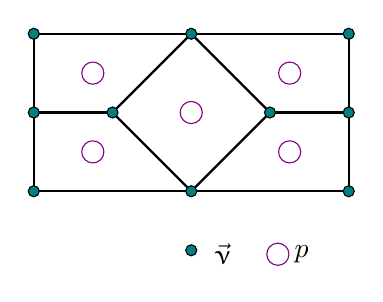
\begin{tikzpicture}
%\draw[fill=gray!23,gray!23](0,0) rectangle (5,5);
%\draw[step=0.5cm,gray,very thin] (0,0) grid (6,4); %background grid
\draw[thick] (1,1) -- (5,1) -- (5,3) -- (1,3) -- cycle;  
\draw[thick] (3,1) -- (4,2) -- (3,3) -- (2,2) -- cycle;  
\draw[thick] (1,2) -- (2,2);  
\draw[thick] (4,2) -- (5,2);  

\draw[black,fill=teal] (1,1) circle (2pt);
\draw[black,fill=teal] (3,1) circle (2pt);
\draw[black,fill=teal] (5,1) circle (2pt);
\draw[black,fill=teal] (1,2) circle (2pt);
\draw[black,fill=teal] (2,2) circle (2pt);
\draw[black,fill=teal] (4,2) circle (2pt);
\draw[black,fill=teal] (5,2) circle (2pt);
\draw[black,fill=teal] (1,3) circle (2pt);
\draw[black,fill=teal] (3,3) circle (2pt);
\draw[black,fill=teal] (5,3) circle (2pt);

\draw[violet] (1.75,1.5) circle (4pt);
\draw[violet] (1.75,2.5) circle (4pt);
\draw[violet] (4.25,1.5) circle (4pt);
\draw[violet] (4.25,2.5) circle (4pt);
\draw[violet] (3,2) circle (4pt);

\draw[black,fill=teal] (3,0.25)   circle (2pt);
\node[] at (3.4,0.2) {$\vec\upnu$};

\draw[violet] (4.1,0.2) circle (4pt); 
\node[] at (4.4,0.2) {$p$};

\end{tikzpicture}
\end{center}




Gresho \& Sani \cite{grsa} state: "For fans of $Q_1\times Q_0$ who want 
guaranteed optimal convergence of both $u$ and $p$ (with however larger error 
constants caused by the distorted shapes?), one way to assure this is
to discretise via the macro elements above, each composed of five $Q_1\times Q_0$
quadrilaterals. Such checkerboard-killer meshes have been employed in practice
by (at least) Bath\'e \cite{chba93}. Both the macro-element and the proof are
due to Stenberg \cite{sten84}."

Chapelle \& Bathe \cite{chba93}: "the numerical inf-sup test is passed for this mesh and in fact,
this behavior was proven analytically (see Brezzi \& Fortin \cite{brfo}, see 
also Le Tallec \& Ruas \cite{leru86}).

\begin{center}
\includegraphics[width=5cm]{images/meshtopos/qizh07}\\
{\captionfont Taken from Qin \& Zhang (2007) \cite{qizh07}.}
\end{center}

Implemented in \stone~78.

\Literature: Fig 3.12 of Elman \etal book \cite{elsw}.

%......................................
\subsubsection{The Le Tallec macro-element} 

This macro-element is introduced in Le Tallec (1981) \cite{leta81}.

\begin{flushright} {\tiny {\color{gray} (tikz\_letallec.tex)}} \end{flushright}
%~~~~~~~~~~~~~~~~~~~~~~~~~~~~~~~~~~~~~~~~~~~~~~~~~~~~~~~~~~~~~~~~~~~~~~~~~~~~~~~~~~~~~~~~~~~~~~~~~~

\begin{center}
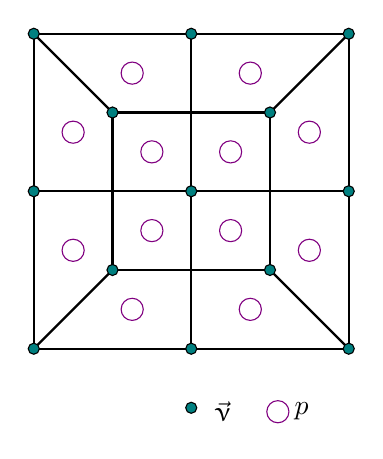
\begin{tikzpicture}
%\draw[fill=gray!23,gray!23](0,0) rectangle (5,5);
%\draw[step=0.5cm,gray,very thin] (0,0) grid (6,6); %background grid
\draw[thick] (1,1) -- (5,1) -- (5,5) -- (1,5) -- cycle;  
\draw[thick] (2,2) -- (4,2) -- (4,4) -- (2,4) -- cycle;  

\draw[thick] (1,1) -- (2,2);  
\draw[thick] (5,1) -- (4,2);  
\draw[thick] (1,5) -- (2,4);  
\draw[thick] (5,5) -- (4,4);  
\draw[thick] (1,3) -- (5,3);  
\draw[thick] (3,1) -- (3,5);  

\draw[black,fill=teal] (1,1)   circle (2pt);
\draw[black,fill=teal] (3,1)   circle (2pt);
\draw[black,fill=teal] (5,1)   circle (2pt);

\draw[black,fill=teal] (2,2)   circle (2pt);
\draw[black,fill=teal] (4,2)   circle (2pt);

\draw[black,fill=teal] (1,3)   circle (2pt);
\draw[black,fill=teal] (3,3)   circle (2pt);
\draw[black,fill=teal] (5,3)   circle (2pt);

\draw[black,fill=teal] (2,4)   circle (2pt);
\draw[black,fill=teal] (4,4)   circle (2pt);

\draw[black,fill=teal] (1,5)   circle (2pt);
\draw[black,fill=teal] (3,5)   circle (2pt);
\draw[black,fill=teal] (5,5)   circle (2pt);

\draw[violet] (2.25,1.5) circle (4pt);
\draw[violet] (3.75,1.5) circle (4pt);

\draw[violet] (1.5,2.25) circle (4pt);
\draw[violet] (1.5,3.75) circle (4pt);
\draw[violet] (2.5,2.5) circle (4pt);
\draw[violet] (3.5,2.5) circle (4pt);
\draw[violet] (2.5,3.5) circle (4pt);
\draw[violet] (3.5,3.5) circle (4pt);
\draw[violet] (4.5,2.25) circle (4pt);
\draw[violet] (4.5,3.75) circle (4pt);
\draw[violet] (2.25,4.5) circle (4pt);
\draw[violet] (3.75,4.5) circle (4pt);

\draw[black,fill=teal] (3,0.25)   circle (2pt);
\node[] at (3.4,0.2) {$\vec\upnu$};

\draw[violet] (4.1,0.2) circle (4pt); 
\node[] at (4.4,0.2) {$p$};

\end{tikzpicture}\\
\end{center}




This macro-element has been proven stable in \cite{leta81,leru86}, i.e. it satisfies 
the stability condition (see Section~\ref{ss:pair}).
It is also mentioned in Qin \& Zhang (2007) \cite{qizh07}.

Implemented in \stone 78.

%..............................................
\subsubsection{The Qin \& Zhang macro-elements}

In their paper Qin \& Zhang (2007) \cite{qizh07} the authors mention the Stenberg and Le Tallec
macro-elements and also introduce three new ones:

\begin{minipage}{0.31\textwidth}
\begin{flushright} {\tiny {\color{gray} (tikz\_qizh07a.tex)}} \end{flushright}
%~~~~~~~~~~~~~~~~~~~~~~~~~~~~~~~~~~~~~~~~~~~~~~~~~~~~~~~~~~~~~~~~~~~~~~~~~~~~~~~~~~~~~~~~~~~~~~~~~~

\begin{center}
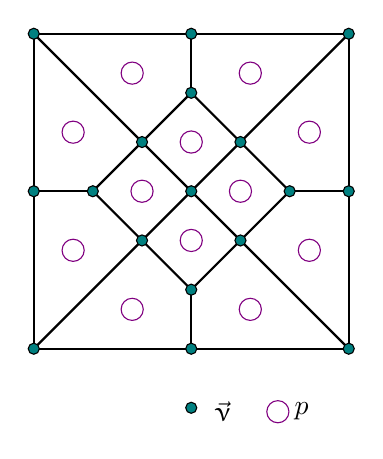
\begin{tikzpicture}
%\draw[fill=gray!23,gray!23](0,0) rectangle (5,5);
%\draw[step=0.5cm,gray,very thin] (0,0) grid (6,6); %background grid
\draw[thick] (1,1) -- (5,1) -- (5,5) -- (1,5) -- cycle;  
\draw[thick] (1.75,3) -- (3,1.75) -- (4.25,3) -- (3,4.25) -- cycle;  

\draw[thick] (1,1) -- (5,5) ;  
\draw[thick] (1,5) -- (5,1) ;  

\draw[thick] (3,1) -- (3,1.75) ;  
\draw[thick] (3,4.25) -- (3,5) ;  

\draw[thick] (1,3) -- (1.75,3) ;  
\draw[thick] (4.25,3) -- (5,3) ;  

\draw[black,fill=teal] (1,1)   circle (2pt);
\draw[black,fill=teal] (3,1)   circle (2pt);
\draw[black,fill=teal] (5,1)   circle (2pt);

\draw[black,fill=teal] (3,1.75)   circle (2pt);
\draw[black,fill=teal] (2.375,2.375)   circle (2pt);
\draw[black,fill=teal] (3.625,2.375)   circle (2pt);

\draw[black,fill=teal] (1,3)   circle (2pt);
\draw[black,fill=teal] (1.75,3)   circle (2pt);
\draw[black,fill=teal] (3,3)   circle (2pt);
\draw[black,fill=teal] (4.25,3)   circle (2pt);
\draw[black,fill=teal] (5,3)   circle (2pt);

\draw[black,fill=teal] (2.375,3.625)   circle (2pt);
\draw[black,fill=teal] (3.625,3.625)   circle (2pt);
\draw[black,fill=teal] (3,4.25)   circle (2pt);

\draw[black,fill=teal] (1,5)   circle (2pt);
\draw[black,fill=teal] (3,5)   circle (2pt);
\draw[black,fill=teal] (5,5)   circle (2pt);

\draw[violet] (2.25,1.5) circle (4pt);
\draw[violet] (3.75,1.5) circle (4pt);

\draw[violet] (1.5,2.25) circle (4pt);
\draw[violet] (3,2.375) circle (4pt);
\draw[violet] (4.5,2.25) circle (4pt);

\draw[violet] (2.375,3) circle (4pt);
\draw[violet] (3.625,3) circle (4pt);

\draw[violet] (3,3.625) circle (4pt);
\draw[violet] (1.5,3.75) circle (4pt);
\draw[violet] (4.5,3.75) circle (4pt);

\draw[violet] (2.25,4.5) circle (4pt);
\draw[violet] (3.75,4.5) circle (4pt);

\draw[black,fill=teal] (3,0.25)   circle (2pt);
\node[] at (3.4,0.2) {$\vec\upnu$};

\draw[violet] (4.1,0.2) circle (4pt); 
\node[] at (4.4,0.2) {$p$};
\end{tikzpicture}\\
\end{center}


\end{minipage}\hfill 
\begin{minipage}{0.31\textwidth}
\begin{flushright} {\tiny {\color{gray} (tikz\_qizh07b.tex)}} \end{flushright}
%~~~~~~~~~~~~~~~~~~~~~~~~~~~~~~~~~~~~~~~~~~~~~~~~~~~~~~~~~~~~~~~~~~~~~~~~~~~~~~~~~~~~~~~~~~~~~~~~~~

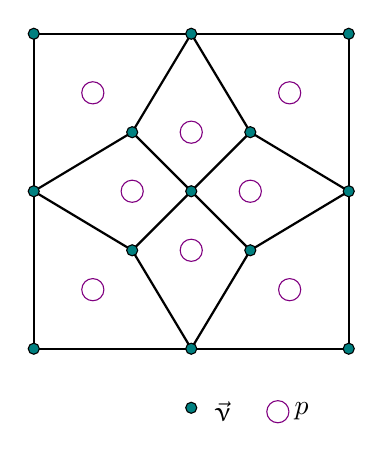
\begin{tikzpicture}

%\draw[fill=gray!23,gray!23](0,0) rectangle (5,5);
%\draw[step=0.5cm,gray,very thin] (0,0) grid (6,6); %background grid
\draw[thick] (1,1) -- (5,1) -- (5,5) -- (1,5) -- cycle;  
\draw[thick] (1,3) -- (2.25,2.25) -- (3,1) -- (3.75,2.25) -- (5,3) --(3.75,3.75) -- (3,5) --(2.25,3.75) --cycle;  
\draw[thick] (2.25,2.25) -- (3.75,3.75) ;  %diags
\draw[thick] (2.25,3.75) -- (3.75,2.25) ;  

\draw[black,fill=teal] (1,1)   circle (2pt); %perimeter nodes
\draw[black,fill=teal] (3,1)   circle (2pt);
\draw[black,fill=teal] (5,1)   circle (2pt);
\draw[black,fill=teal] (1,3)   circle (2pt);
\draw[black,fill=teal] (3,3)   circle (2pt);
\draw[black,fill=teal] (5,3)   circle (2pt);
\draw[black,fill=teal] (1,5)   circle (2pt);
\draw[black,fill=teal] (3,5)   circle (2pt);
\draw[black,fill=teal] (5,5)   circle (2pt);

\draw[black,fill=teal] (2.25,2.25)   circle (2pt); %inside nodes
\draw[black,fill=teal] (3.75,3.75)   circle (2pt);
\draw[black,fill=teal] (2.25,3.75)   circle (2pt);
\draw[black,fill=teal] (3.75,2.25)   circle (2pt);

\draw[violet] (1.75,1.75) circle (4pt);
\draw[violet] (4.25,1.75) circle (4pt);
\draw[violet] (4.25,4.25) circle (4pt);
\draw[violet] (1.75,4.25) circle (4pt);

\draw[violet] (3,2.25) circle (4pt);
\draw[violet] (3,3.75) circle (4pt);
\draw[violet] (2.25,3) circle (4pt);
\draw[violet] (3.75,3) circle (4pt);

%------------------------------------------
\draw[black,fill=teal] (3,0.25)   circle (2pt);
\node[] at (3.4,0.2) {$\vec\upnu$};
\draw[violet] (4.1,0.2) circle (4pt); 
\node[] at (4.4,0.2) {$p$};


\end{tikzpicture}\\

\end{minipage}\hfill 
\begin{minipage}{0.31\textwidth}
\begin{flushright} {\tiny {\color{gray} (tikz\_qizh07c.tex)}} \end{flushright}
%~~~~~~~~~~~~~~~~~~~~~~~~~~~~~~~~~~~~~~~~~~~~~~~~~~~~~~~~~~~~~~~~~~~~~~~~~~~~~~~~~~~~~~~~~~~~~~~~~~


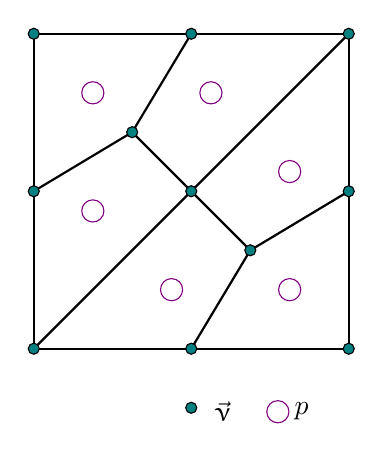
\begin{tikzpicture}
%\draw[fill=gray!23,gray!23](0,0) rectangle (5,5);
%\draw[step=0.5cm,gray,very thin] (0,0) grid (6,6); %background grid
\draw[thick] (1,1) -- (5,1) -- (5,5) -- (1,5) -- cycle;  
\draw[thick] (1,3) -- (2.25,3.75) -- (3,5);
\draw[thick] (3,1) -- (3.75,2.25) -- (5,3);
\draw[thick] (1,1) -- (5,5) ;  %diags
\draw[thick] (2.25,3.75) -- (3.75,2.25) ;  

\draw[black,fill=teal] (1,1)   circle (2pt); %perimeter nodes
\draw[black,fill=teal] (3,1)   circle (2pt);
\draw[black,fill=teal] (5,1)   circle (2pt);
\draw[black,fill=teal] (1,3)   circle (2pt);
\draw[black,fill=teal] (3,3)   circle (2pt);
\draw[black,fill=teal] (5,3)   circle (2pt);
\draw[black,fill=teal] (1,5)   circle (2pt);
\draw[black,fill=teal] (3,5)   circle (2pt);
\draw[black,fill=teal] (5,5)   circle (2pt);

\draw[black,fill=teal] (2.25,3.75)   circle (2pt); %inside nodes
\draw[black,fill=teal] (3.75,2.25)   circle (2pt);

\draw[violet] (4.25,1.75) circle (4pt);
\draw[violet] (1.75,4.25) circle (4pt);

\draw[violet] (2.75,1.75) circle (4pt);
\draw[violet] (4.25,3.25) circle (4pt);
\draw[violet] (1.75,2.75) circle (4pt);
\draw[violet] (3.25,4.25) circle (4pt);

%------------------------------------------
\draw[black,fill=teal] (3,0.25)   circle (2pt);
\node[] at (3.4,0.2) {$\vec\upnu$};
\draw[violet] (4.1,0.2) circle (4pt); 
\node[] at (4.4,0.2) {$p$};
\end{tikzpicture}


\end{minipage}

They also indicate that although stable, these macro-elements are inferior 
to the above two (Stenberg \& Le Tallec). 

%..............................................
\subsubsection{New macro-elements ?}

\begin{center}
\includegraphics[width=4cm]{images/meshtopos/m21}
\includegraphics[width=4cm]{images/meshtopos/m22}
\end{center}

I came up with these, no idea whether these are stable/usable or better than the others.






 

 %---------------
 %%%%%%%%%%%%%%%%%%%%%%%%%%%%%%%%%%%%%%%%%%%%%%%%%%%%%%%%%%%%%%%%%%%%%%%%%%%%%%%%

%%%%%%%%%%%%%%%%%%%%%%%%%%%%%%%%%%%%%%%%%%%%%%%%%%%%%%%%%%%%%%%%%%%%%%%%%%%%%%%%%%%%%%%%%%%%%%%%%%%
%\chapter{The Discontinuous Galerkin Finite Element Method (DG-FEM) \label{dgfem}} %%%%%%%%%%%%%%%%
\chapter{The Discontinuous Galerkin Finite Element Method (DG-FEM) \label{dgfem}} %%%%%%%%%%%%%%%%%

\begin{flushright} {\tiny {\color{gray} chapter7.tex}} \end{flushright}


Books:

\begin{itemize}
\item {\it Discontinuous Galerkin Methods. Theory, Computation and Applications} by
Cockburn, Karniadakis and Shu \cite{cockburn00}
\item {\it Mathematical Aspects of Discontinuous Galerkin Methods} by Di Pietro and Ern 
\cite{dipietro_ern12}
\item {\it Discontinuous Galerkin Methods. Analysis and Applications to Compressible Flow} by 
Dolejsi and Feistauer \cite{dolejsi_feistauer15}
\item {\it Discontinuous Galerkin Methods for Solving Elliptic and Parabolic Equations} by Rivi{\'e}re
\cite{riviere08}
\item {\it Discontinuous finite elements in fluid dynamics and heat transfer} by Li \cite{li06}
\item {\it Nodal Discontinuous Galerkin Methods. Algorithms, Analysis, and Applications} by 
Hesthaven \& Warbuton \cite{hewa08}
\end{itemize}


There are many different flavours of the Discontinuous Galerkin Finite Element Method:
\begin{itemize}
\item {\bf HDG}: Hybridizable DG \cite{conp10}
\item {\bf IIPG}: incomplete interior penalty G  \cite{dole08}
\item {\bf LDG}: Local DG \cite{cacp02}  
\end{itemize}


\section{First-order advection ODE in 1D} 

%------------------------------------------
\subsection{First-order advection ODE in 1D}

What follows is borrowed from the book "Discontinuous finite elements in fluid dynamics and heat
transfer" by Ben Q. Li \cite{li06}.

To illustrate the basic ideas of the discontinuous finite element method, we
consider a simple, one-dimensional, first order differential equation with $u$
specified at one of the boundaries:
\begin{equation}
\frac{du}{dx} + g =0 \qquad x\in[a,b] \qquad \text{and} \qquad u(x=a)=u_a
\end{equation}
where $g$ is a constant (for simplicity).
The domain is discretized such that : $\Omega_j = [x_j,x_{j+1}]$ with $j = 1, 2, ..., nel$.
Then, integrating the above equation over the element $j$ with respect to a weighting function $f(x)$
\begin{equation}
\int_{x_j}^{x_{j+1}} \left( \frac{d u}{dx} + g \right) f(x) dx = 0
\end{equation}
Remembering that $\int_c^d u(x)v'(x) dx = [u(x)v(x)]_c^d - \int_c^d u'(x)v(x) dx$, 
we can now perform an integration by parts on the differential operator and we obtain:
\begin{equation}
[u(x)f(x)]_{x_j}^{x_{j+1}}  -\int_{x_j}^{x_{j+1}} \left( u \frac{d f}{dx} - g f(x)\right)  dx = 0
\end{equation}
or, 
\begin{equation}
u(x_{j+1})f(x_{j+1}) 
- u(x_{j})f(x_{j}) 
-\int_{x_j}^{x_{j+1}} \left( u \frac{d f}{dx} - g f(x)\right)  dx = 0
\end{equation}


On $\Omega_j$ $u$ is approximated by $u_h \in H$, $H$ being an appropriate function
space of finite dimension, and $f$ by $f_h$ taken from the same function space as $u_h$. 
Upon substituting $(u_h , f_h )$ for $(u,f)$ in the equation above, we have
the discontinuous Galerkin finite element formulation:
\begin{equation}
u_h(x_{j+1}) f_h(x_{j+1}) - u_h(x_{j})f_h(x_{j}) 
-\int_{x_j}^{x_{j+1}} \left( u_h \frac{d f_h}{dx} - g f_h(x)\right)  dx = 0
\end{equation}

In the continuous finite element approach, the field variable $u_h$ is forced to be
continuous across the boundary.
The essential idea for the discontinuous method is
that $u_h$ is allowed to be discontinuous across the boundary. Therefore, across the
element, the following two different values are defined at the two sides of the
boundary:
\begin{equation}
u_j^+ = \lim_{x \searrow x_j^+} u_h(x)
\qquad
u_j^- = \lim_{x \nearrow x_j^-} u_h(x)
\end{equation}

\begin{center}
\includegraphics[width=4cm]{images/dgfem/dgfem_1}\\
{\scriptsize An illustration of the jump across $x_j$ of element $j$: 
$x_j$ and $x_{j+1}$ mark the
boundaries of the element}
\end{center}

Conversely, we also have:
\begin{equation}
u_{j+1}^+ = \lim_{x \searrow x_{j+1}^+} u_h(x)
\qquad
u_{j+1}^- = \lim_{x \nearrow x_{j+1}^-} u_h(x)
\end{equation}



It is key to remember that 1) $u_h$ is discontinuous only at the element boundaries; 
2) the solution $u$ is smooth within (but excluding) the boundary. 
By this definition, the above equation contains the variables only within the integral limits of $\Omega_j$ . 
As a consequence, there is no direct coupling with other intervals or other elements. 
{\sl The field values at a node, or the interface between two elements, are not unique}. They are
calculated using the two limiting values approaching the interface from the two
adjacent elements. This feature is certainly desirable for problems with internal
discontinuities.

We can now write CHECK CHECK
\begin{equation}
u_{j+1}^- f_h(x_{j+1}) - u_j^+ f_h(x_{j}) 
-\int_{x_j}^{x_{j+1}} \left( u_h \frac{d f_h}{dx} - g f_h(x)\right)  dx = 0
\end{equation}
and we can integrate by parts again the term which contains a derivative:
\[
\int_{x_j}^{x_{j+1}} u_h(x) \frac{d f_h}{dx} dx = [u_h f_h] -  \int_{x_j}^{x_{j+1}} f_h(x) \frac{d u_h}{dx} dx 
\]

and then 
\begin{equation}
u_{j+1}^- f_h(x_{j+1}) - u_j^+ f_h(x_{j}) 
-\int_{x_j}^{x_{j+1}} \left( u_h \frac{d f_h}{dx} - g f_h(x)\right)  dx = 0
\end{equation}




\newpage
We start from the simplest ODE:
\[
\frac{du}{dx}=1  \qquad x\in[0,2] \qquad \text{and} \qquad u(x=0)=0
\]
As in the Continuous Galerkin case, the function $f$ is replaced by a shape function $N_i(x)$:



How the hell do I arrive at:
\[
\int_{x_j}^{x_{j+1}} \left( \frac{d u_h}{dx} + g(u_h) \right) N_i(x) dx + (u_j^+-u_j^-) N_i(x_j) = 0
\]

\newpage
%------------------------------------------
\subsection{Steady state diffusion in 1D}

Let us start simple with the 1D steady state heat conduction problem in 1D, given by the following 
equation:
\begin{equation}
\frac{d^2T}{dx^2}=0 \qquad T(x=0)=0 \qquad T(x=1)=1 \qquad \text{on} \quad x\in[0,1]
\end{equation}
Although this equation is usually solved as is with its second-order derivative, it can also 
be written in a mixed form:
\[
-\frac{dq}{dx}=0 \qquad q-\frac{dT}{dx}=0 \qquad x\in[0,1]
\]
and the boundary conditions remain unchanged. 

We apply the standard approach to establish the weak forms of these two first-order ODEs, and we do so 
on an element $e$ bound by $x_j$ and $x_{j+1}$
\[
-\int_{x_j}^{x_{j+1}} \frac{dq}{dx} \tilde{N}(x) dx = -[q \tilde{N} ]_{x_j}^{x_{j+1}} 
+ \int_{x_j}^{x_{j+1}} \frac{d\tilde{N}}{dx} q(x) dx = 0
\]
\[
\int_{x_j}^{x_{j+1}}  \left( q-\frac{dT}{dx} \right) \overline{N}(x) dx
=
\int_{x_j}^{x_{j+1}}  q(x) \overline{N}(x) dx
-[ q \overline{N}  ]_{x_j}^{x_{j+1}} + \int_{x_j}^{x_{j+1}} \frac{d\tilde{N}}{dx} T(x) dx = 0
\]
We now must examine the term between square brackets. 
Inside the element, the test functions $\tilde{N}$ and $\overline{N}$ are well defined polynomials
and we we coin:
\[
\tilde{N}_j^+=\tilde{N}(x_j^+)
\qquad
\tilde{N}_{j+1}^-=\tilde{N}(x_{j+1}^-)
\qquad
\qquad
\overline{N}_j^+=\overline{N}(x_j^+)
\qquad
\overline{N}_{j+1}^-=\overline{N}(x_{j+1}^-)
\]
where $N$ is the number of nodes.
Concerning $q$ and $T$, we will for now  give them values $\hat{q}_j$ and $\hat{T}_j$ at node $j$
and $\hat{q}_{j+1}$ and $\hat{T}_{j+1}$ at node $j+1$, and we will specify the hat quantities as follows:

\begin{eqnarray}
\hat{T}_j &=&
\left\{
\begin{array}{ll}
T_j^-   & j=1 \\ 
\frac{1}{2}(T_j^-+T_j^+) + {\cal C} (T_j^- - T_j^+) & j=2,...N-1\\
T_j^+    & j=N \\ 
\end{array}
\right. \nonumber\\
\hat{q}_j &=&
\left\{
\begin{array}{ll}
q_j^+ -{\cal E} (T_j^--T_j^+)  & j=1 \\ 
\frac{1}{2}(q_j^+ + q_j^-) - {\cal E} (T_j^- - T_j^+) - {\cal C}(q_j^- - q_j^+) & j=2,...N-1\\
q_j^- -{\cal E} (T_j^--T_j^+)    & j=N \\ 
\end{array}
\right.
\end{eqnarray}
where ${\cal C}$ and ${\cal E}$ are two constants. 

Inside an element bounded by nodes $k$ and $k+1$, 
the temperature $T$ and heat flux $q$ are interpolated over an isoparametric linear element:
\[
T_h(r) = N_1(r) T_k^+ + N_2(r)T_{k+1}^-
\]
\[
q_h(r) = N_1(r) q_k^+ + N_2(r)q_{k+1}^-
\]
As in the (Continuous) Galerkin case of section~\ref{sec:diff1D}, the test functions are taken to 
be the shape functions, and in this case for both temperature and flux. 










\section{Steady state diffusion in 1D \label{ss:dgss1D}} \input{dgfem1D_ssdiff}
\section{Time-dependent diffusion PDE in 1D} \begin{flushright} {\tiny {\color{gray} dgfem1D\_diff.tex}} \end{flushright}
%~~~~~~~~~~~~~~~~~~~~~~~~~~~~~~~~~~~~~~~~~~~~~~~~~~~~~~~~~~~~~~~~~~~~~~~~~~~~~~~~~~~~~~~~~~~~~~~~~~

Starting from the simple transient 1-D heat conduction problem similar to the 
steady state heat conduction problem only with added time dependence:

\begin{equation}
\frac{\partial T}{\partial t}=\frac{\partial^2T}{\partial x^2} \qquad T(x=0)=0 \qquad T(x=1)=1 \qquad \text{on} \quad x\in[0,1]
\end{equation}

Once again we split this system into two seperate first order equations:
\begin{eqnarray}
\frac{\partial T}{\partial t}-\frac{\partial q}{\partial x}&=&0 \nn\\
\frac{\partial T}{\partial x} -q &=& 0
\end{eqnarray}

We apply the standard approach to establish the weak forms of these two first-order PDEs, and we do so 
on an element $e$ bound by nodes $k$ and $k+1$ with coordinates $x_k$ and $x_{k+1}$
\begin{eqnarray}
-\int_{x_k}^{x_{k+1}} \left( \frac{\partial T}{\partial t}- \frac{dq}{dx} \right) \tilde{f}(x) dx =
\int_{x_k}^{x_{k+1}} \frac{\partial T}{\partial t} \tilde{f}(x)dx
 -\left[q \tilde{f} \right]_{x_k}^{x_{k+1}} 
+ \int_{x_k}^{x_{k+1}} \frac{d\tilde{f}}{dx} q(x) dx &=& 0
\label{eq:dg1a}\\
\int_{x_k}^{x_{k+1}}  \left( q-\frac{dT}{dx} \right) \overline{f}(x) dx
=
\int_{x_k}^{x_{k+1}}  q(x) \overline{f}(x) dx
-\left[ T \overline{f}  \right]_{x_k}^{x_{k+1}} + \int_{x_k}^{x_{k+1}} \frac{d\overline{f}}{dx} T(x) dx 
&=& 0
\label{eq:dg2a}
\end{eqnarray}
where $\tilde{f}$ and $\overline{f}$ are test functions.

In what follows we coin $\dot{T}=\partial T/\partial t$ (for convenience of notation). 
We once again recover Equations (\ref{eq:dgq1}) and (\ref{eq:dgT1}), although with 
an additional time derivative term. 

Filling this into equations (\ref{eq:dgq1}) and (\ref{eq:dgT1}), gives 
\begin{eqnarray}
{\bm K}^e \cdot 
\left( 
\begin{array}{cc}
    {\color{red}q_k^+}  \\
    {\color{red}q_{k+1}^-}
\end{array}
\right)
+
{\bm M}^e \cdot 
\left(
\begin{array}{c}
{\color{red}\dot{T}_k^+}  \\
{\color{red}\dot{T}_{k+1}^-} 
\end{array}
\right) 
+ 
\left(
\begin{array}{cc}
     ({\cal C}+\frac{1}{2})  {\color{red}q_k^+}  \\
     ({\cal C}-\frac{1}{2})  {\color{red}q_{k+1}^-} 
\end{array}
\right)+
\left(
\begin{array}{c}
     {\cal E}    {\color{red}T_k^+}  \\
     {\cal E}    {\color{red}T_{k+1}^-} 
\end{array}
\right) 
&=& 
\left(
\begin{array}{cc}
     ({\cal C}-\frac{1}{2}) q_k^-  \\
     ({\cal C}+\frac{1}{2}) q_{k+1}^+ 
\end{array}
\right)
+ \left(
\begin{array}{cc}
     {\cal E}   T_k^-  \\
     {\cal E}   T_{k+1}^+
\end{array}
\right)  
\nn
\\
{\bm M}^e \cdot
\left(
\begin{array}{cc}
    {\color{red}q_k^+}  \\
    {\color{red}q_{k+1}^-}
\end{array}
\right)+
{\bm K}^e \cdot
\left(
\begin{array}{cc}
 {\color{red}T_k^+}  \\
{\color{red}T_{k+1}^-} 
\end{array}
\right) 
+ \left(
\begin{array}{cc}
     (\frac{1}{2}-{\cal C}) {\color{red}T_k^+}  \\
     -({\cal C}+\frac{1}{2}){\color{red}T_{k+1}^-} 
\end{array}
\right)
&=& \left(
\begin{array}{cc}
     -({\cal C}+\frac{1}{2})  T_k^- \\
     (\frac{1}{2}-{\cal C})  T_{k+1}^+ 
\end{array}
\right) 
\end{eqnarray}

In what follows we set ${\cal E}=0$ so that we have
\begin{eqnarray}
{\bm K}^e \cdot 
\left( 
\begin{array}{cc}
    {\color{red}q_k^+}  \\
    {\color{red}q_{k+1}^-}
\end{array}
\right)
+
{\bm M}^e \cdot 
\left(
\begin{array}{c}
{\color{red}\dot{T}_k^+}  \\
{\color{red}\dot{T}_{k+1}^-} 
\end{array}
\right) 
+ 
\left(
\begin{array}{cc}
     ({\cal C}+\frac{1}{2})  {\color{red}q_k^+}  \\
     ({\cal C}-\frac{1}{2})  {\color{red}q_{k+1}^-} 
\end{array}
\right)
&=& 
\left(
\begin{array}{cc}
     ({\cal C}-\frac{1}{2}) q_k^-  \\
     ({\cal C}+\frac{1}{2}) q_{k+1}^+ 
\end{array}
\right)
\nn
\\
{\bm M}^e \cdot
\left(
\begin{array}{cc}
    {\color{red}q_k^+}  \\
    {\color{red}q_{k+1}^-}
\end{array}
\right)+
{\bm K}^e \cdot
\left(
\begin{array}{cc}
 {\color{red}T_k^+}  \\
{\color{red}T_{k+1}^-} 
\end{array}
\right) 
+ \left(
\begin{array}{cc}
     (\frac{1}{2}-{\cal C}) {\color{red}T_k^+}  \\
     -({\cal C}+\frac{1}{2}){\color{red}T_{k+1}^-} 
\end{array}
\right)
&=& \left(
\begin{array}{cc}
     -({\cal C}+\frac{1}{2})  T_k^- \\
     (\frac{1}{2}-{\cal C})  T_{k+1}^+ 
\end{array}
\right) 
\end{eqnarray}

Using the expressions for ${\bm M}^e$ and ${\bm K}^e$ 
obtained in Appendix~\ref{app:mm} for 1D linear elements we arrive at
\begin{eqnarray}
\frac{1}{2}
\left(
\begin{array}{cc}
-1  & -1 \\
1 & 1
\end{array}
\right)
\cdot 
\left( 
\begin{array}{cc}
    {\color{red}q_k^+}  \\
    {\color{red}q_{k+1}^-}
\end{array}
\right)
+
\frac{h}{6}
\left(
\begin{array}{cc}
2  & 1 \\
1 & 2
\end{array}
\right)
\cdot 
\left(
\begin{array}{c}
{\color{red}\dot{T}_k^+}  \\
{\color{red}\dot{T}_{k+1}^-} 
\end{array}
\right) 
+ 
\left(
\begin{array}{cc}
     ({\cal C}+\frac{1}{2})  {\color{red}q_k^+}  \\
     ({\cal C}-\frac{1}{2})  {\color{red}q_{k+1}^-} 
\end{array}
\right)
&=& 
\left(
\begin{array}{cc}
     ({\cal C}-\frac{1}{2}) q_k^-  \\
     ({\cal C}+\frac{1}{2}) q_{k+1}^+ 
\end{array}
\right)
\nn
\\
\frac{h}{6}
\left(
\begin{array}{cc}
2  & 1 \\
1 & 2
\end{array}
\right)
\cdot
\left(
\begin{array}{cc}
    {\color{red}q_k^+}  \\
    {\color{red}q_{k+1}^-}
\end{array}
\right)+
\frac{1}{2}
\left(
\begin{array}{cc}
-1  & -1 \\
1 & 1
\end{array}
\right)
\cdot
\left(
\begin{array}{cc}
 {\color{red}T_k^+}  \\
{\color{red}T_{k+1}^-} 
\end{array}
\right) 
+ \left(
\begin{array}{cc}
     (\frac{1}{2}-{\cal C}) {\color{red}T_k^+}  \\
     -({\cal C}+\frac{1}{2}){\color{red}T_{k+1}^-} 
\end{array}
\right)
&=& \left(
\begin{array}{cc}
     -({\cal C}+\frac{1}{2})  T_k^- \\
     (\frac{1}{2}-{\cal C})  T_{k+1}^+ 
\end{array}
\right) 
\end{eqnarray}

which simplifies to 
\begin{eqnarray}
\left(
\begin{array}{cc}
C  & -1/2 \\
1/2 & C 
\end{array}
\right)
\cdot 
\left( 
\begin{array}{cc}
    {\color{red}q_k^+}  \\
    {\color{red}q_{k+1}^-}
\end{array}
\right)
+
\left(
\begin{array}{cc}
h/3 & h/6 \\
h/6 & h/3
\end{array}
\right)
\cdot 
\left(
\begin{array}{c}
{\color{red}\dot{T}_k^+}  \\
{\color{red}\dot{T}_{k+1}^-} 
\end{array}
\right) 
&=& 
\left(
\begin{array}{cc}
     ({\cal C}-\frac{1}{2}) q_k^-  \\
     ({\cal C}+\frac{1}{2}) q_{k+1}^+ 
\end{array}
\right)
\nn
\\
\left(
\begin{array}{cc}
h/3 & h/6 \\
h/6 & h/3
\end{array}
\right)
\cdot
\left(
\begin{array}{cc}
    {\color{red}q_k^+}  \\
    {\color{red}q_{k+1}^-}
\end{array}
\right)+
\left(
\begin{array}{cc}
-C  & -1/2 \\
1/2 & -C
\end{array}
\right)
\cdot
\left(
\begin{array}{cc}
 {\color{red}T_k^+}  \\
{\color{red}T_{k+1}^-} 
\end{array}
\right) 
&=& \left(
\begin{array}{cc}
     -({\cal C}+\frac{1}{2})  T_k^- \\
     (\frac{1}{2}-{\cal C})  T_{k+1}^+ 
\end{array}
\right) 
\end{eqnarray}
or, 
\[
{\bm C}_1 \vec{q} +  {\bm M} \vec{\dot{T}} = \vec{f}  
\]
\[
{\bm M} \vec{q} + {\bm C}_2 \vec{T} = \vec{g}
\]
so 
\[
 \vec{q} = {\bm M}^{-1}   (\vec{g} -  {\bm C}_2 \vec{T} )
\]
and then 
\[
{\bm C}_1 [  {\bm M}^{-1}   (\vec{g} -  {\bm C}_2 \vec{T} )   ]    +  {\bm M} \vec{\dot{T}} = \vec{f}  
\]


NOT REALLY FINISHED...










































































%\end{document}




\newpage
\section{Time-dependent advection PDE in 1D \label{ss:dgfem1D_adv}} Starting from the 1-D advection equation:
\begin{equation}
    \frac{\partial T}{\partial t}+u\frac{\partial T}{\partial x}=0 
\end{equation}
where $T$ is the temperature and $u$ the velocity. 
As shown before we start by discretizing the domain into a collection of elements. Then the above equation can be integrated over the element which is bounded by nodes $x_k$ and $x_{k+1}$. 

\begin{equation}
\int_{x_k}^{x_{k+1}}  \left(\frac{\partial T}{\partial t}+u\frac{\partial T}{\partial x}\right) \tilde{f}(x) dx 
=
\int_{x_k}^{x_{k+1}} \tilde{f}(x)\frac{\partial T}{\partial t} dx
+\left[ uT \tilde{f}  \right]_{x_k}^{x_{k+1}}
-\int_{x_k}^{x_{k+1}} \frac{\partial \tilde{f}}{\partial x} uT dx
=0 \nn
\end{equation}
with the test function $\tilde{f}$. 
Inside the elements the test functions are defined by well defined polynomials. 
We once again define
\[
\tilde{f}_k^+=\tilde{f}(x_k^+)
\qquad
\tilde{f}_{k+1}^-=\tilde{f}(x_{k+1}^-)
\]
\begin{equation}
    \int_{x_k}^{x_{k+1}}\left(
    \tilde{f}(x)\frac{\partial T_h}{\partial t}-
    \frac{\partial \tilde{f}}{\partial x} uT_h \right) dx
    +\tilde{f}(x_{k+1})\widehat{uT}(T_{k+1}^-,T_{k+1}^+)
    -\tilde{f}(x_{k})\widehat{uT}(T_{k}^-,T_{k}^+)=0
    \label{1Dcond}
\end{equation}
For a constant $u$ or a linear problem, an effective numerical flux
is the Lax-Friedrichs flux:
\index{general}{Lax-Friedrichs flux}
\begin{equation}
\widehat{uT}(a,b)=u \frac{(a+b)}{2}-|u|\frac{(b-a)}{2}
\end{equation}
when $u>0$ this flux then simply becomes:
\begin{equation}
uT(a,b)=u a
\end{equation}
which is in essence an upwinding scheme.
Filling this into equation \ref{1Dcond} gives:
\begin{equation}
\int_{x_k}^{x_{k+1}}\left(
\tilde{f}(x)\frac{\partial T_h}{\partial t}-
\frac{\partial \tilde{f}}{\partial x} uT_h \right) dx
+\tilde{f}_{k+1}^-uT_{k+1}^-     -\tilde{f}_{k}^-uT_{k}^-=0
\end{equation}
The function $T_h$ inside the element can be approximated 
as follows:
\begin{equation}
T_h(x) = \sum_{i=1}^m N_i(x) T_i = 
N_k(x) {\color{red}T_k^+} + N_{k+1}(x) {\color{red}T_{k+1}^-}
\label{eq:dgadv1} 
\end{equation}
In what follows we coin $\dot{T}=\partial T/\partial t$ so
\begin{equation}
\dot{T}_h(x) 
= \sum_{i=1}^m N_i(x) \dot{T}_i 
= N_k(x) {\color{red}\dot{T}_k^+} + N_{k+1}(x) {\color{red}\dot{T}_{k+1}^-}
\label{eq:dgadv2} 
\end{equation}
Taking $\tilde{f}(x)=N_k(x)$ and then $\tilde{f}(x)=N_{k+1}(x)$ we arrive at
\begin{eqnarray}
\int_{x_k}^{x_{k+1}}\left(
N_k(x) \dot{T}_h -
\frac{\partial N_k}{\partial x} uT_h \right) dx
+\underbrace{N_k(x_{k+1}^-)}_{=0}u {\color{red}T_{k+1}^-}     - \underbrace{N_k (x_{k}^-)}_{=1}uT_{k}^- &=& 0 \\
\int_{x_k}^{x_{k+1}}\left(
N_{k+1}(x) \dot{T}_h -
\frac{\partial N_{k+1}}{\partial x} uT_h \right) dx
+ \underbrace{N_{k+1}(x_{k+1}^-)}_{1}u {\color{red}T_{k+1}^-}     -\underbrace{N_{k+1}(x_{k}^-)}_{=0}uT_{k}^- &=& 0
\end{eqnarray}
i.e.
\begin{eqnarray}
\int_{x_k}^{x_{k+1}}\left(
N_k(x) \dot{T}_h -
\frac{\partial N_k}{\partial x} uT_h \right) dx
   -  uT_{k}^- &=& 0 \\
\int_{x_k}^{x_{k+1}}\left(
N_{k+1}(x)  \dot{T}_h -
\frac{\partial N_{k+1}}{\partial x} uT_h \right) dx
+ u{\color{red} T_{k+1}^-}      &=& 0
\end{eqnarray}
We now use Eqs.~(\ref{eq:dgadv1}) and (\ref{eq:dgadv2})
\begin{eqnarray}
\int_{x_k}^{x_{k+1}}\left(
N_k
[N_k {\color{red}\dot{T}_k^+} + N_{k+1} {\color{red}\dot{T}_{k+1}^-}]
-
\frac{\partial N_k}{\partial x} u
[N_k {\color{red}T_k^+} + N_{k+1} {\color{red}T_{k+1}^-}]
 \right) dx
   -  uT_{k}^- &=& 0 \\
\int_{x_k}^{x_{k+1}}\left(
N_{k+1} 
[N_k {\color{red}\dot{T}_k^+} + N_{k+1} {\color{red}\dot{T}_{k+1}^-}]
 -
\frac{\partial N_{k+1}}{\partial x} u
[N_k {\color{red}T_k^+} + N_{k+1} {\color{red}T_{k+1}^-}]
\right) dx
+ u{\color{red} T_{k+1}^-}      &=& 0
\end{eqnarray}
Defining again (see Appendix~\ref{app:mm})
\[
{\bm M}_e=
\int_{x_k}^{x_{k+1}}
\left(
\begin{array}{cc}
N_kN_k & N_k N_{k+1} \\
N_{k+1}N_k & N_{k+1} N_{k+1} 
\end{array}
\right)
dx
= 
\frac{h}{6}
\left(
\begin{array}{cc}
2  & 1 \\
1 & 2
\end{array}
\right)
\]
and 
\[
{\bm K}^e =
\int_{\Omega_e} 
\left(
\begin{array}{cc}
\frac{dN_k}{dx} N_k     & \frac{dN_k}{dx} N_{k+1} \\
\frac{dN_{k+1}}{dx} N_k & \frac{dN_{k+1}}{dx} N_{k+1}
\end{array}
\right)
dV
=
\frac{1}{2}
\left(
\begin{array}{cc}
-1  & -1 \\
1 & 1
\end{array}
\right)
\]
This results in:
\begin{eqnarray}
{\bm M}_e 
\cdot
\left(
\begin{array}{cc}
{\color{red}\dot T_k^+}  \\
{\color{red} \dot T_{k+1}^-} 
\end{array}
\right) 
-u {\bm K}_e \cdot \left(
\begin{array}{cc}
     {\color{red}T_k^+}  \\
     {\color{red}T_{k+1}^-} 
\end{array}
\right) + 
u
\left( 
\begin{array}{cc}
0 & 0 \\
0 & 1 
\end{array}
\right)
\cdot
\left( 
\begin{array}{c}
0   \\
{\color{red}T_{k+1}^-} 
\end{array}
\right)
-\left(
\begin{array}{cc}
     u{T_{k}^-}   \\
     0 
\end{array}
\right)=0
\end{eqnarray}
or,
\begin{eqnarray}
{\bm M}_e \cdot
\left(
\begin{array}{cc}
{\color{red}\dot T_k^+}  \\
{\color{red} \dot T_{k+1}^-} 
\end{array}
\right) 
=
u \left[ {\bm K}_e -
\left(\begin{array}{cc}
0 & 0 \\
0 & 1 
\end{array}\right)
\right] \cdot 
\left( \begin{array}{cc}
{\color{red}T_k^+}  \\
{\color{red}T_{k+1}^-} 
\end{array} \right) 
+u \left( \begin{array}{cc}
{T_{k}^-}   \\  0 
\end{array} \right)
\end{eqnarray}


\begin{eqnarray}
{\bm M}_e \cdot
\left(
\begin{array}{cc}
{\color{red}\dot T_k^+}  \\
{\color{red} \dot T_{k+1}^-} 
\end{array}
\right) 
=
u\frac{1}{2}  
\left(\begin{array}{cc}
-1 & -1 \\
1 & -1 
\end{array}\right)
 \cdot 
\left( \begin{array}{cc}
{\color{red}T_k^+}  \\
{\color{red}T_{k+1}^-} 
\end{array} \right) 
+u \left( \begin{array}{cc}
{T_{k}^-}   \\  0 
\end{array} \right)
\end{eqnarray}

\begin{eqnarray}
\left(
\begin{array}{cc}
{\color{red}\dot T_k^+}  \\
{\color{red} \dot T_{k+1}^-} 
\end{array}
\right) 
=
u
{\bm M}_e^{-1} \cdot\frac{1}{2}  
\left(\begin{array}{cc}
-1 & -1 \\
1 & -1 
\end{array}\right)
 \cdot 
\left( \begin{array}{cc}
{\color{red}T_k^+}  \\
{\color{red}T_{k+1}^-} 
\end{array} \right) 
+u 
{\bm M}_e^{-1} \cdot
\left( \begin{array}{cc}
{T_{k}^-}   \\  0 
\end{array} \right)
\end{eqnarray}
We have already established that 
\[
{\bm M}_e^{-1} = 
\frac{2}{h}
\left( 
\begin{array}{cc}
2 & -1 \\
-1 & 2
\end{array}
\right)
\]
so 
\begin{eqnarray}
\boxed{
\left(
\begin{array}{cc}
{\color{red}\dot T_k^+}  \\
{\color{red} \dot T_{k+1}^-} 
\end{array}
\right)=
\frac{u}{h} 
\left(\begin{array}{cc}
    -3 & -1 \\
     3 & -1
\end{array}
\right)
\left(
\begin{array}{cc}
{\color{red}T_k^+}  \\
{\color{red}T_{k+1}^-} 
\end{array}
\right) + \frac{u}{h} \left(
\begin{array}{cc}
4   \\
-2 
\end{array}
\right)T_k^-  
}
\end{eqnarray}

Using the same first order Runge-Kutta method as in the previous section, 
\begin{equation}
T^k(t+\delta t)=T_k(t) +\delta t \; \dot{T}_k
\end{equation}
we multiply the equation by $\delta t$ and we obtain 
\begin{eqnarray}
\left(
\begin{array}{cc}
{\color{blue} T_k^+}(t+\delta t)  \\
{\color{blue}T_{k+1}^-} (t+\delta t) 
\end{array}
\right)=
 \left(
\begin{array}{cc}
{\color{blue} T_k^+} (t) \\
{\color{blue}T_{k+1}^-} (t) 
\end{array}
\right)+
\frac{u \delta t}{h} 
\left(\begin{array}{cc}
    -3 & -1 \\
     3 & -1
\end{array}
\right)
\left(
\begin{array}{cc}
{\color{blue}T_k^+} (t) \\
{\color{blue}T_{k+1}^-} (t)
\end{array}
\right) + 
\frac{u \delta t}{h} \left(
\begin{array}{cc}
     4   \\
     -2 
\end{array}
\right)T_k^- (t+\delta t) 
\end{eqnarray}
and finally
\begin{mdframed}[backgroundcolor=blue!5]
\begin{eqnarray}
\left(
\begin{array}{cc}
{\color{blue} T_k^+}(t+\delta t)  \\
{\color{blue}T_{k+1}^-} (t+\delta t) 
\end{array}
\right)=
\left[
{\bm 1} + 
\frac{u \delta t}{h} 
\left(\begin{array}{cc}
    -3 & -1 \\
     3 & -1
\end{array}
\right)
\right]\cdot
\left(
\begin{array}{cc}
{\color{blue}T_k^+} (t) \\
{\color{blue}T_{k+1}^-} (t)
\end{array}
\right) + 
\frac{u \delta t}{h} \left(
\begin{array}{cc}
     4   \\
     -2 
\end{array}
\right)T_k^- (t+\delta t) 
\end{eqnarray}
\end{mdframed}







This problem can be solved starting from the left boundary and sweeping through all the elements. The updated values of adjacent elements are used in the calculation of the next element as soon as this element becomes available which is why 
the last term $T_k^-$ is taken  at $t+\delta t$.
 %-------

\newpage
\section{Steady-state diffusion in 2D} 
Let us start from the 2D steady state heat diffusion equation:
\begin{equation}
    \vec{\nabla} \cdot k \vec{\nabla} T + H=0
\end{equation}
Just as in the 1D case this equation can be split in two separate first order differential equations:
\begin{equation}
    \underbrace{-\vec{\nabla}\cdot \vec{q} + H=0}_{\text{ODE 1}} \quad ; \quad \underbrace{\vec{q}=-k\vec{\nabla } T}_{\text{ODE 2}}
\end{equation}
Let $N^\uptheta_i$ be the temperature basis functions so that the temperature inside an element is given by
\begin{equation}
T_h (\vec{r}) = \sum_{i=1}^m N_i^\uptheta (\vec{r}) \; T_i = \vec{N^\uptheta}\cdot \vec{T}
\end{equation}
where $\vec{T}$ is a vector of length $m$, the number of nodes per element. Similarly we let the basis function for the heat flux be
\begin{equation}
\qhx(x,y) = \sum_{i=1}^m N_i^q (x,y) \qix = \vec{N^q}\cdot \vec{\qx}
\end{equation}
\begin{equation}
\qhy(x,y) = \sum_{i=1}^m N_i^q (x,y) \qiy = \vec{N^q}\cdot \vec{\qy}
\end{equation}
where $\vec{\qx}$, $\vec{\qy}$ and $\vec{N}^q$ 
are vectors of length $m$ too. Implicitly if $m$ is the same for temperature and heat flux, then $N^\uptheta = N^q$.

Let us establish the weak forms of the 1st order ODEs. 


\paragraph{ODE 1} This results in:
\begin{eqnarray}
\int_\Omega {N^\uptheta_i} \vec{\nabla} \cdot \vec{q} \; dV = \int_\Omega {N^\uptheta_i} H \; dV
\label{eq:SSD2D}
\end{eqnarray}
Using the product rule which states:
\[
\vec{\nabla} \cdot ({N^\uptheta_i}\vec{q})={N^\uptheta_i}\vec{\nabla} \cdot \vec{q} 
+ \vec{\nabla}{N^\uptheta_i} \cdot \vec{q} 
\qquad
\Rightarrow
\qquad
{N^\uptheta_i}\vec{\nabla} \cdot \vec{q}=\vec{\nabla} \cdot ({N^\uptheta_i}\vec{q})- 
\vec{\nabla}{N^\uptheta_i} \cdot \vec{q}
\]
which we insert in Eq.~(\ref{eq:SSD2D}) results in 
\begin{equation}
\int_{\Omega} \vec{\nabla} \cdot ({N^\uptheta_i} \vec{q}) dV - 
\int_{\Omega} \vec{\nabla} {N^\uptheta_i} \cdot \vec{q} dV = \int_{\Omega} {N^\uptheta_i} H dV
\label{eq:SSD2D1}
\end{equation}
Using the divergence theorem 
$\int_\Omega \vec{\nabla} \cdot \vec{F} \; d\Omega = \int_{d\Omega}(\vec{F} \cdot \vec{n}) \; dS$ 
 applied to Eq.~(\ref{eq:SSD2D1}) leads to
\begin{equation}
\int_{d\Omega}{N^\uptheta_i} \vec{\hat{q}} \cdot \vec{n} \; dS  - 
\int_{\Omega} \vec{\nabla} {N^\uptheta_i} \cdot \vec{q} \; dV = 
\int_{\Omega} {N^\uptheta_i} H  \; dV
\end{equation}

Here $\vec{n}$ is the outward vector everywhere on the boundary. 
The exact solution $\vec{q}=(\qx,\qy)$ can be approximated with $\vec{q}_h$ in a  finite element space, same for the approximation of the flux at the boundary $\hat{q}=\hat{q_h}$ which takes a special form in the context of the DG methods (as reflected by the presence of the hat).
\begin{equation}
\underbrace{ \int_{d\Omega}{N^\uptheta_i} \vec{\hat{q_h}} \cdot \vec{n} \; dS}_{A } - 
\underbrace{ \int_{\Omega} \vec{\nabla} {N^\uptheta_i} \cdot \vec{q_h} \; dV}_{B} = 
\underbrace{\int_{\Omega} {N^\uptheta_i} H  \;dV }_C
\label{eq:q2dss}
\end{equation}
%To make things very explicit, we can split the heat flux in its $x$ and $y$ component in the above equation:
%\begin{equation}
%\int_{d\Omega}  {N^\theta} (\hat{\qx} \nx + \hat{\qy} \ny) \; dS  -  
%\int_{\Omega} ( \partial_x N^\theta \qx   + 
%\partial_y N^\theta \qy ) \; dV = 
%\int_{\Omega} {N^\theta} H dV
%\label{eq:q2dss}
%\end{equation}
The middle and right terms are explained in Section~\ref{ss:hte_diff}, 
so we will focus on the left term only (i.e. the one with the fluxes).
In all what follows blue symbols belong the the element under consideration 
and brown symbols belong to its neighbour(s).

\includegraphics[width=5cm,angle=90]{images/dgfem/elts}
%Here the blue color (before: $el$ superscript) indicates that it belongs to the element of interest and brown color (before: the $nb$ superscript) 
%denotes the values belonging to the neighbouring element. 
$\vec{n}^+$ indicates the outward vector at the boundary and $\vec{n}^-$ is 
the outward vector of the neighbouring element.

Let us turn to the book for useful definitions:
\begin{itemize}
\item
\underline{Definition of jump operators} The square brackets denote the jump operator:
\begin{eqnarray}
[\vec{q}_h] &=& \vec{\color{blue}q}_h \cdot \vec{n}^+ 
+ \vec{\color{brown} q}_h \cdot \vec{n}^- 
\qquad \text{or} \qquad 
[\vec{q}_h]= (\vec{\color{blue}q}_h - \vec{\color{brown}q}_h) \cdot \vec{n}^+    \nn\\
\left[T_h\right] &=& \blueT_h \vec{n}^+ + {\brownT}_h \vec{n}^-  \qquad \text{or} \qquad 
[T_h]=(\blueT_h  - \brownT_h ) \; \vec{n}^+ 
\end{eqnarray}
%[q_{h,x}]=q_{h,x}^{el}n_x^+ + q_{h,x}^{nb}n_x^- \nn \\
%[q_{h,y}]=q_{h,y}^{el}n_y^+ + q_{h,y}^{nb}n_y^- \nn \\

Note that $[\vec{q}_h]$ is a scalar function which involves the
normal components only; while $[T_h]$ is a vector function. 

\item
\underline{Definition of average operators} The curly brackets indicate the average operator
\begin{eqnarray}
\{ \vec{q}_h \}&=&\frac{1}{2}(\vec{\color{blue}q}_h + \vec{\color{brown}q}_h)
\qquad \text{so} \quad 
\{\qhx\}=\frac{1}{2}(\blueqx_h + \brownqx_h) 
\qquad \text{and}
\qquad  \{\qhy\}=\frac{1}{2}(\blueqy_h + \brownqy_h) \nn \\
\{T_h\}&=&\frac{1}{2}(\blueT_h + \brownT_h) \nn 
\end{eqnarray}
Note that $\{ \vec{q}_h \}$ is a vector, while 
$\{T_h\}$ is a scalar.

\item
\underline{Definitions of fluxes} In the LDG method the boundary flux $\vec{\hat{q}}$ is defined as 
\[
\vec{\hat{q_h}} = \{ \vec{q_h} \} -{\cal{E}} [T_h]- \vec{\cal{C}}  [\vec{q_h}] 
\]
where ${\cal{E}}$ is a scalar (since $[T_h]$ is a vector)
and $\vec{\cal C}$ is a vector (since $[\vec{q}_h]$ is a scalar).
To be once again very explicit:
\begin{eqnarray}
\hat{\qhx} 
&=& \{\qhx\} -{\cal{E}} [T_h]_x- {\cal{C}}_x  [\vec{q}_h] \nn\\
&=& \frac{1}{2}(\blueqx_h + \brownqx_h)
-{\cal{E}} (\blueT_h {n}_x^+ + \brownT_h {n}_x^-)
-{\cal{C}}_x  
(\vec{\color{blue}q}_h \cdot \vec{n}^+ +\vec{\color{brown}q}_h \cdot \vec{n}^-) \label{flux2Da}\\
\hat{\qhy} 
&=& \{\qhy\} -{\cal{E}} [T_h]_y- {\cal{C}}_y  [\vec{q}_h] \nn\\
&=& \frac{1}{2}(\blueqy_h + \brownqy_h)  
-{\cal{E}}  (\blueT_h {n}_y^+ + \brownT_h {n}_y^-)
-{\cal{C}}_y  (\vec{\color{blue} q}_h \cdot \vec{n}^+ +\vec{\color{brown}q}_h \cdot \vec{n}^-) \label{flux2Db}
\end{eqnarray}

\begin{remark}
Note that in the the book the note under table 4.1 states that the $C_{ij}$ 
coefficients are constant matrices, which is quite misleading since some are actually scalars and others vectors.
\end{remark}

\end{itemize}


Filling Eqs.~(\ref{flux2Da},\ref{flux2Db}) into Eq.~(\ref{eq:q2dss}) leads to
%(note that I have introduced the upperscript + on the normal components 
%because the integration is on the boundary of the element - does that make sense?)


\begin{eqnarray}
A&=& \int_{\partial\Omega} N^\uptheta_i \vec{\hat{q_h}} \cdot \vec{n} \; dS \nn\\ 
&=&
\int_{\partial\Omega} N^\uptheta_i \left[ \{ \vec{q_h} \} -{\cal{E}} [T_h]- \vec{\cal{C}}  [\vec{q_h}] \right] \cdot \vec{n}^+ \; dS  \nn\\
&=&
\int_{\partial\Omega}{N^\uptheta_i} \left[ \frac{1}{2}(\vec{\color{blue}q}_h + \vec{\color{brown}q}_h) 
-{\cal{E}} (\blueT_h \vec{n}^+ + \brownT_h \vec{n}^-)- \vec{\cal{C}}  [\vec{q_h}] \right] \cdot \vec{n}^+ \; dS  \nn\\
&=&
\int_{\partial\Omega}{N^\uptheta_i} \left[ \frac{1}{2}(\vec{\color{blue}q}_h + \vec{\color{brown}q}_h)\cdot\vec{n}^+ 
  -{\cal{E}} (\blueT_h \vec{n}^+ + \brownT_h \vec{n}^-) \cdot \vec{n}^+
- \vec{\cal{C}} \cdot \vec{n}^+ [\vec{q_h}] \right] \; dS  \nn\\
&=&
\int_{\partial\Omega}{N^\uptheta_i} \left[ \frac{1}{2}(\vec{\color{blue}q}_h + \vec{\color{brown}q}_h)\cdot\vec{n}^+  -{\cal{E}} (\blueT_h -\brownT_h ) 
- (\vec{\cal{C}} \cdot \vec{n}^+) 
(\vec{\color{blue}q}_h - \vec{\color{brown}q}_h) \cdot \vec{n}^+
\right] \; dS  \qquad \text{since} \quad  \vec{n}^+\!\cdot\!\vec{n}^+ =1 \quad  \vec{n}^+\!\cdot\!\vec{n}^- =-1 \nn\\
&=&
\int_{\partial\Omega}{N^\uptheta_i} \left[
\left(\frac{1}{2} - \vec{\cal{C}} \cdot \vec{n}^+ \right) \vec{\color{blue}q}_h\cdot\vec{n}^+
- {\cal{E}} \blueT_h
\right] \; dS 
+ 
\int_{\partial\Omega}{N^\uptheta_i} \left[
\left(\frac{1}{2} + \vec{\cal{C}} \cdot \vec{n}^+ \right)
\vec{\color{brown}q}_h \cdot\vec{n}^+
+ {\cal{E}} \brownT_h
\right] \; dS  \nn \\
&=&
\int_{\partial\Omega}{N^\uptheta_i} 
\left(\frac{1}{2} - \vec{\cal{C}} \cdot \vec{n}^+ \right) \vec{\color{blue}q}_h\cdot\vec{n}^+ \; dS 
- \int_{\partial\Omega}{N^\uptheta_i}  {\cal{E}} \blueT_h  \; dS 
+ 
\int_{\partial\Omega}{N^\uptheta_i} \left(\frac{1}{2} + \vec{\cal{C}} \cdot \vec{n}^+ \right)
\vec{\color{brown}q}_h \cdot\vec{n}^+   \; dS
+
\int_{\partial\Omega}{N^\uptheta_i}   {\cal{E}} \brownT_h   \; dS  \nn \\
&=& A_1 + A_2 + A_3 + A_4 
\end{eqnarray}
In order to simplify notations we choose $N^q=N^\uptheta=N$ and drop the $h$ subscripts.

\begin{eqnarray}
A_1 
&=& \int_{\partial\Omega}{N_i} \left(\frac{1}{2} - \vec{\cal{C}} \cdot \vec{n}^+ \right) \vec{\color{blue}q}\cdot\vec{n}^+ \; dS \nn \\
&=& \int_{\partial\Omega}{N_i} \left(\frac{1}{2} - \vec{\cal{C}} \cdot \vec{n}^+ \right) ({\color{blue}q}_x n^+_x  +   {\color{blue}q}_y {n}_y^+) \; dS \nn \\
&=& \int_{\partial\Omega}{N_i} \left(\frac{1}{2} - \vec{\cal{C}} \cdot \vec{n}^+ \right) {\color{blue}q}_x n^+_x   \; dS 
+ \int_{\partial\Omega}{N_i} \left(\frac{1}{2} - \vec{\cal{C}} \cdot \vec{n}^+ \right)  {\color{blue}q}_y {n}_y^+ \; dS \nn \\
\Rightarrow {\vec A}_1
&=& \left( \int_{\partial\Omega}  \left(\frac{1}{2} - \vec{\cal{C}} \cdot \vec{n}^+ \right) \vec{N}^T \vec{N} n^+_x  \; dS  \right) \cdot {\color{blue}\vec{\qx}}  
+ \left( \int_{\partial\Omega}  \left(\frac{1}{2} - \vec{\cal{C}} \cdot \vec{n}^+ \right) \vec{N}^T \vec{N} n^+_y  \; dS  \right) \cdot {\color{blue}\vec{\qy}}  \\
A_2 &=& - \int_{\partial\Omega}{N_i}  {\cal{E}} \blueT  \; dS \nn\\
\Rightarrow {\vec A}_2 &=& - \left( \int_{\partial\Omega}   {\cal{E}}   \vec{N}^T \vec{N} dS \right) \cdot \vec{\blueT} \\
A_3 
&=& \int_{\partial\Omega}{N^\uptheta_i} \left(\frac{1}{2} + \vec{\cal{C}} \cdot \vec{n}^+ \right)
 \vec{\color{brown}q} \cdot\vec{n}^+   \; dS \nn\\
&=& \int_{\partial\Omega}{N^\uptheta_i} \left(\frac{1}{2} + \vec{\cal{C}} \cdot \vec{n}^+ \right)
 ({\color{brown}q}_x {n}_x^+  +  {\color{brown}q}_y {n}_y^+       )  \; dS \nn\\
&=& 
\int_{\partial\Omega}{N^\uptheta_i} \left(\frac{1}{2} + \vec{\cal{C}} \cdot \vec{n}^+ \right)  {\color{brown}q}_x {n}_x^+    \; dS 
+ \int_{\partial\Omega}{N^\uptheta_i} \left(\frac{1}{2} + \vec{\cal{C}} \cdot \vec{n}^+ \right)   {\color{brown}q}_y {n}_y^+    \; dS \nn\\
\Rightarrow {\vec A}_3 &=&
  \left(\int_{\partial\Omega} \left(\frac{1}{2} + \vec{\cal{C}} \cdot \vec{n}^+ \right) \vec{N}^T \vec{N} {n}_x^+    \; dS \right) \cdot  {\color{brown}\vec{\qx}}
+ \left(\int_{\partial\Omega} \left(\frac{1}{2} + \vec{\cal{C}} \cdot \vec{n}^+ \right) \vec{N}^T \vec{N} {n}_y^+    \; dS \right) \cdot  {\color{brown}\vec{\qy}} \\
A_4 &=& \int_{\partial\Omega}{N_i}   {\cal{E}}  \brownT   \; dS  \nn\\
\Rightarrow {\vec A}_4 &=&  \left( \int_{\partial\Omega}   {\cal{E}}   \vec{N}^T \vec{N} dS \right) \cdot \vec{\brownT} \\ 
B 
&=& \int_{\Omega} \vec{\nabla} {N_i} \cdot \vec{\color{blue} q} \; dV  \nn \\
&=& \int_{\Omega} (\partial_x N_i {\color{blue}q}_x + \partial_y N_i {\color{blue}q}_y )   \; dV  \nn \\
&=& \int_{\Omega} \partial_x N_i {\color{blue}q}_x   \; dV   
 +  \int_{\Omega} \partial_y N_i {\color{blue}q}_y   \; dV  \nn \\
\Rightarrow {\vec B} &=& 
  \left(\int_{\Omega} \partial_x \vec{N}^T \vec{N}   \; dV \right)\cdot {\color{blue}\vec{\qx}}  
+ \left(\int_{\Omega} \partial_y \vec{N}^T \vec{N}   \; dV \right)\cdot {\color{blue}\vec{\qy}}  \\
C &=& \int_{\Omega} {N_i} H  \;dV \nn \\
\Rightarrow {\vec C} &=& \int_{\Omega} \vec{N}^T H  \;dV  
\end{eqnarray}


The expressions above find their equivalent in the book (NB stands for neighbour):
\begin{center}
\includegraphics[width=11cm]{images/dgfem/li_01}\\
{\captionfont Note that in the book we have: $C_{12}={\bm C}_{12}\cdot {\bm n}^+ \rightarrow \vec{\cal C}\cdot\vec{n}^+$;
$C_{11} \rightarrow {\cal E}$}
\end{center}






%---------------------------------------------------
\paragraph{ODE 2} The weak form of Ode \#2 writes:

\[
\int_\Omega N_i^q (\vec{q} + k\vec{\nabla } T ) dV = 0
\]
or, (once again we drop the superscript on the shape functions and the $h$):
\[
\int_\Omega N_i \vec{q} \;  dV + \int_\Omega N_i k\vec{\nabla } T \; dV = 0
\]
We then use $\int_\Omega \vec\nabla f \; dV = \int_{\partial\Omega} f \vec{dS}$
and as before the temperature on the edge integral should be $\hat{T}$:
\[
\int_\Omega N_i \vec{q} \;  dV + \int_{\partial\Omega}  k N_i \hat{T} \; \vec{n}^+  dS - \int_\Omega \vec\nabla (k N_i)   T \; dV = 0
\]


or, if decomposed in a 2D Cartesian axis system 
\begin{eqnarray}
0
%&=&\int_\Omega N_i \left( \qx + k  \frac{\partial T}{\partial x} \right) \; dV \nn\\
%&=&\int_\Omega N_i  \qx^h dV
%+ \int_\Omega N_i k  \frac{\partial T^h}{\partial x}  \; d\Omega \nn\\
&=&\int_\Omega N_i  \qx dV 
+\int_{\partial\Omega} N_i k \hat{T} \; n^+_x dS
-\int_\Omega \partial_x ( k N_i) \;  T \; dV \nn\\
0
%&=&\int_\Omega N_i \left( \qy^h + k  \frac{\partial T^h}{\partial y} \right) \; dV \nn\\
%&=&\int_\Omega N_i  \qy^h dV
%+ \int_\Omega N_i k  \frac{\partial T^h}{\partial y}  \; d\Omega \nn\\
&=&\int_\Omega N_i  \qy^h dV 
+\int_{\partial\Omega} N_i k \hat{T} \; n^+_y dS
-\int_\Omega \partial_y (k N_i) \;  T \; dV \nn
\end{eqnarray}
%Both can be summed together and creating the vector $\vec{N}=(N_i,N_i)= N_i(\vec{e}_x+\vec{e}_y)$ then we get 
%\[
%\int_\Omega \vec{N}_i \cdot \vec{q}^h dV 
%+\int_{\partial\Omega} k \hat{T} \vec{N}\cdot \vec{n}^+  dS
%-\int_\Omega \vec{\nabla}\cdot (\vec{N}_i k) \;  T \; dV 
%=0
%\]
which (aside from a minus sign coming from a different definition of the heat flux) is 'identical' to the book
(although the notations in the book are hella confusing):
\begin{center}
\includegraphics[width=8cm]{images/dgfem/li_02} (with $\kappa \rightarrow k$, ${\bm w}\rightarrow \vec{N}$)
\end{center}


\begin{eqnarray}
D &=&  \\
E &=&  \\
F &=&  \\
G &=&  \\
H &=&  \\
I &=&  \\
\end{eqnarray}
























\par\noindent\rule{\textwidth}{0.4pt}


We start from the steady state (no advection) energy equation:
\[
\vec\nabla\cdot (k \vec\nabla T) + Q = 0
\]
where $Q$ is a source term.
As we did in 1D we tranform this equation by reintroducing the heat flux
\footnote{\url{https://en.wikipedia.org/wiki/Thermal_conduction}} $\vec{q}$ 
\begin{eqnarray}
\vec q &=& - k \vec\nabla T \\
\vec\nabla \cdot \vec q &=& Q
\end{eqnarray}
We then multiply these two equations with the test functions $\vec{N}_q$ (this one 
is vector valued) and 
$N_T$ respectively and integrate over the element $e$ under consideration:
\begin{eqnarray}
\int_{\Omega_e} \vec{N}_q \cdot  \vec q  \; dV &=& - \int_{\Omega_e} \vec{N}_q \cdot k \vec\nabla T\; dV \\
\int_{\Omega_e} N_T \vec\nabla \cdot \vec q \;  dV &=& \int_{\Omega_e} N_T Q \; dV
\end{eqnarray}
We then use integration by parts to make fluxes appear (and assume $k$ is constant within 
the element). We have
\begin{eqnarray}
\int_{\Omega_e} \vec{N}_q \cdot k \vec\nabla T \; dV 
&=& \int_{\Gamma_e} kT \;  \vec{N}_q \cdot \vec{n} \; dS 
- \int _{\Omega_e}  kT \;  \vec\nabla\cdot \vec{N}_q  \;  dV \\
\int_{\Omega_e} N_T \vec\nabla \cdot \vec q \; dV 
&=& \int_{\Gamma_e} {N}_T \vec{q} \cdot \vec{n}  \; dS
- \int_{\Omega_e} \vec\nabla N_T \cdot \vec q \; dV 
\end{eqnarray}
We then finally obtain the weak forms that are to be discretised:
\begin{eqnarray}
\int_{\Omega_e} \vec{N}_q \cdot  \vec q \; dV &=& 
-\int_{\Gamma_e} kT \;  \vec{N}_q \cdot \vec{n} \; dS 
+ \int _{\Omega_e}  kT \;  \vec\nabla\cdot \vec{N}_q  \;  dV \\
\int_{\Gamma_e}    {N}_T  \vec{q}\cdot \vec{n}  \; dS
- \int_{\Omega_e} \vec\nabla N_T \cdot \vec q \; dV 
&=& \int_{\Omega_e} N_T Q \; dV
\end{eqnarray}

We seek to approximate the exact solution $(\vec{q},T)$ with functions $(\vec{q}_h,T_h)$ inside the element so we 
now have 
\begin{eqnarray}
\int_{\Omega_e} \vec{N}_q \cdot  \vec q_h \; dV &=& 
-\int_{\Gamma_e} k \hat{T}_h \;  \vec{N}_q \cdot \vec{n} \; dS 
+ \int _{\Omega_e}  k T_h \;  \vec\nabla\cdot \vec{N}_q  \;  dV \\
\int_{\Gamma_e}    {N}_T \hat{\vec{q}}_h \cdot \vec{n}  \; dS
- \int_{\Omega_e} \vec\nabla N_T \cdot \vec{q}_h \; dV 
&=& \int_{\Omega_e} N_T Q \; dV
\end{eqnarray}
where the numerical fluxes are the approximations to $(\vec{q},T)$ on the boundary of element $e$.
As before we must now specify these fluxes inside the domain and also on the boundaries. These
can obviously not be chosen at will since they must at least render the discontinuous formulation stable.



The following table is taken from Li \cite{li06} and lists the numerical fluxes 
that are considered consistent and stable for the solution of the steady state heat conduction 
problems \cite{arbc02,cacp00}:
\begin{center}
\begin{tabular}{lll}
\hline
Method & $\hat{\vec{q}}_h$ & $\hat{T}_h$ \\
\hline
LDG \cite{cosh98} & $\{ \vec{q}_h \}$  & \\
DG  \cite{cacp00} & \\
Brezzi et al (2000) \cite{brmm00} &\\
IP \cite{dodu76} & \\
Bassi-Rebay \cite{barm97} &\\
NIPG \cite{riwg99} & \\
\hline
\end{tabular}
\end{center}
where the $C$ coefficients are matrices ?!



\index{general}{Average Operator}
\index{general}{Jump Operator}
The average operator and jump operators in the table are defined as follows:
let $\Gamma_{12}$ be an interior edge shared by elements $1$ and $2$ and let us 
define the unit normal vectors $\vec{n}_1$ and $\vec{n}_2$ on $\Gamma_{12}$ 
pointing exterior to element 1 and 2, respectively.



\end{document}


\subsection{The special case of linear rectangular elements} 
Let us start with ${\cal A}_e$ where we assume that $k$ is constant within an element:
\begin{eqnarray}
{\cal A}_{\Omega_e}&=&
\left(
\begin{array}{ccc}
{\bm E} & {\bm 0} & {\bm H}_x \\
{\bm 0} & {\bm E} & {\bm H}_y \\
{\bm J}_x & {\bm J}_y & {\bm 0}
\end{array}
\right)
=
\left(
\begin{array}{ccc}
{\bm E} & {\bm 0} & -k_e{\bm J}_x \\
{\bm 0} & {\bm E} & -k_e{\bm J}_y \\
{\bm J}_x & {\bm J}_y & {\bm 0}
\end{array}
\right)
\end{eqnarray}
The matrices ${\bm E}$, ${\bm H}_x$, and ${\bm H}_y$ 
have been analytically derived in Appendix~\ref{app:qrle}:
\begin{scriptsize}
\[
{\bm E}=
\frac{h_x h_y}{9}
\left(
\begin{array}{cccc}
1 & 1/2 & 1/4 & 1/2 \\ 
1/2 & 1   & 1/2 & 1/4 \\ 
1/4 & 1/2 & 1 & 1/2 \\ 
1/2 & 1/4 & 1/2 & 1  
\end{array}
\right)
\qquad
{\bm J}_x=
\frac{h_y}{12} 
\left(
\begin{array}{cccc}
-2 & -2 & -1 & -1 \\
 2 &  2 &  1 & 1 \\
  1 &   1 & 2 & 2 \\
- 1 &  - 1 & -2 & -2
\end{array}
\right)
\qquad
{\bm J}_y=
\frac{h_x}{12} 
\left(
\begin{array}{cccc}
-2 & -1 & -1 & -2 \\
-1 & -2 & -2 & -1  \\
 1 &  2 &  2 &  1  \\
2 & 1 & 1 & 2 
\end{array}
\right) 
\]
\end{scriptsize}
The matrix ${\cal A}_{\Omega_e}$ is therefore trivial to implement. 

Let us now turn to $ {\cal A}_{\partial\Omega}$ which is specific to the DG method.
Because elements are rectangles then $n_i^+n_j^+=0$ if $i \neq j$ (where $i$ and $j$ 
are edge indices). 
Also, if $i=j$ then $n_i^+n_j^+=1$. 

\begin{center}
\includegraphics[width=7cm]{images/dgfem/dgelts_q1}
\end{center}

Assuming here again that heat conductivities are constant inside an element
it then follows that 
\begin{eqnarray}
 {\cal A}_{\partial\Omega_e}
&=&
\sum_{i=1}^{nedges}
\left(
\begin{array}{ccc}
{\bm E}_{xx,i} & {\bm E}_{xy,i} & {\bm H}_{x,i} \\
{\bm E}_{yx,i} & {\bm E}_{yy,i} & {\bm H}_{y,i} \\
{\bm J}_{x,i} & {\bm J}_{y,i} & {\bm G}_{T,i}
\end{array}
\right)
=
\sum_{i=1}^{nedges}
\left(
\begin{array}{ccc}
{\bm E}_{xx,i} & {\bm 0} & {\bm H}_{x,i} \\
{\bm 0} & {\bm E}_{yy,i} & {\bm H}_{y,i} \\
{\bm J}_{x,i} & {\bm J}_{y,i} & {\bm G}_{T,i}
\end{array}
\right)
\end{eqnarray}



Note that 
\begin{itemize}
\item $i=1$: bottom edge, i.e. $s=-1$ and then $N_4=N_3=0$; Also $\vec{n}_x^+=0$, $\vec{n}_y^+=-1$
\item $i=2$: right  edge, i.e.  $r=+1$ and then $N_1=N_4=0$; Also $\vec{n}_x^+=1$, $\vec{n}_y^+=0$
\item $i=3$: top edge, i.e. $s=+1$  and then $N_1=N_2=0$; Also $\vec{n}_x^+=0$, $\vec{n}_y^+=1$
\item $i=4$: left edge, i.e. $r=-1$ and then $N_2=N_3=0$; Also $\vec{n}_x^+=-1$, $\vec{n}_y^+=0$
\end{itemize}

Then 
\begin{eqnarray}
{\bm G}_{T,1} &=& -{\cal{E}} \int_{\partial\Omega_1} \vec{N}^T \vec{N} dS = -  {\cal{E}} {\bm C}_1 \nn\\
{\bm G}_{T,2} &=& -{\cal{E}} \int_{\partial\Omega_2} \vec{N}^T \vec{N} dS = -  {\cal{E}} {\bm C}_2 \nn\\
{\bm G}_{T,3} &=& -{\cal{E}} \int_{\partial\Omega_3} \vec{N}^T \vec{N} dS = -  {\cal{E}} {\bm C}_3 \nn\\
{\bm G}_{T,4} &=& -{\cal{E}} \int_{\partial\Omega_4} \vec{N}^T \vec{N} dS = -  {\cal{E}} {\bm C}_4 \nn
\end{eqnarray}
where the matrices ${\bm C}_i$ have been worked out in detail in appendix~\ref{app:qrle}:
\begin{eqnarray}
{\bm C}_{1} 
&=& \int_{1\rightarrow 2} \vec{N}^T \vec{N} dS  
=
\frac{h_x}{6}
\left(\begin{array}{cccc}
2 & 1 & 0 & 0 \\
1 & 2 & 0 & 0 \\
0 & 0 & 0 & 0 \\
0 & 0 & 0 & 0 
\end{array}\right)
\nn\\
\nn\\
{\bm C}_{2} 
&=& \int_{2\rightarrow 3} \vec{N}^T \vec{N} dS  
=
\frac{h_y}{6}
\left(\begin{array}{cccc}
0 & 0 & 0 & 0 \\
0 & 2 & 1 & 0 \\
0 & 1 & 2 & 0 \\
0 & 0 & 0 & 0 
\end{array}\right)
\nn\\
{\bm C}_{3}
&=& \int_{3\rightarrow 4} \vec{N}^T \vec{N} dS 
=
\frac{h_x}{6}
\left(\begin{array}{cccc}
0 & 0 & 0 & 0 \\
0 & 0 & 0 & 0 \\
0 & 0 & 2 & 1 \\
0 & 0 & 1 & 2 
\end{array}\right)
\nn\\
\nn\\
{\bm C}_{4} 
&=& \int_{4\rightarrow 1} \vec{N}^T \vec{N} dS  
=
\frac{h_y}{6}
\left(\begin{array}{cccc}
2 & 0 & 0 & 1 \\
0 & 0 & 0 & 0 \\
0 & 0 & 0 & 0 \\
1& 0 & 0 & 2 
\end{array}\right)
\nn
\end{eqnarray}

\begin{eqnarray}
{\bm E}_{xx,1} &=& -k_e {\cal F} \int_{\partial\Omega_1}  \vec{N}^T\vec{N}  {n}^+_x   n^+_x dS = 0 \nn\\ 
{\bm E}_{xx,2} &=& -k_e {\cal F} \int_{\partial\Omega_2}  \vec{N}^T\vec{N}  {n}^+_x   n^+_x dS = -k_e {\cal F} {\bm C}_2  \nn\\ 
{\bm E}_{xx,3} &=& -k_e {\cal F} \int_{\partial\Omega_3}  \vec{N}^T\vec{N}  {n}^+_x   n^+_x dS = 0 \nn\\ 
{\bm E}_{xx,4} &=& -k_e {\cal F} \int_{\partial\Omega_4}  \vec{N}^T\vec{N}  {n}^+_x   n^+_x dS = -k_e {\cal F} {\bm C}_4  
\nn\\
{\bm E}_{yy,1} &=& -k_e {\cal F} \int_{\partial\Omega_1}  \vec{N}^T\vec{N}  {n}^+_y   n^+_y dS = -k_e {\cal F} {\bm C}_1  \nn\\ 
{\bm E}_{yy,2} &=& -k_e {\cal F} \int_{\partial\Omega_2}  \vec{N}^T\vec{N}  {n}^+_y   n^+_y dS = 0 \nn\\ 
{\bm E}_{yy,3} &=& -k_e {\cal F} \int_{\partial\Omega_3}  \vec{N}^T\vec{N}  {n}^+_y   n^+_y dS = -k_e {\cal F} {\bm C}_3  \nn\\  
{\bm E}_{yy,4} &=& -k_e {\cal F} \int_{\partial\Omega_4}  \vec{N}^T\vec{N}  {n}^+_y   n^+_y dS = 0 
\nn\\ 
{\bm H}_{x,1} &=& k_e \int_{\partial\Omega_1}  \left( \frac{1}{2} + \vec{\cal C} \cdot \vec{n}^+ \right) \vec{N}^T \vec{N} n^+_x dS = 0 \nn\\ 
{\bm H}_{x,2} &=& k_e \int_{\partial\Omega_2}  \left( \frac{1}{2} + \vec{\cal C} \cdot \vec{n}^+ \right) \vec{N}^T \vec{N} n^+_x dS = k_e  \left( \frac{1}{2} + {\cal C}_x \right) {\bm C}_{2} \nn\\ 
{\bm H}_{x,3} &=& k_e \int_{\partial\Omega_3}  \left( \frac{1}{2} + \vec{\cal C} \cdot \vec{n}^+ \right) \vec{N}^T \vec{N} n^+_x dS = 0 \nn\\ 
{\bm H}_{x,4} &=& k_e \int_{\partial\Omega_4}  \left( \frac{1}{2} + \vec{\cal C} \cdot \vec{n}^+ \right) \vec{N}^T \vec{N} n^+_x dS = - k_e  \left( \frac{1}{2} - {\cal C}_x \right) {\bm C}_{4} 
\nn\\
{\bm H}_{y,1} &=& k_e \int_{\partial\Omega_1}  \left( \frac{1}{2} + \vec{\cal C} \cdot \vec{n}^+ \right) \vec{N}^T \vec{N} n^+_y dS = -k_e  \left( \frac{1}{2} - {\cal C}_y \right) {\bm C}_{1} \nn\\ 
{\bm H}_{y,2} &=& k_e \int_{\partial\Omega_2}  \left( \frac{1}{2} + \vec{\cal C} \cdot \vec{n}^+ \right) \vec{N}^T \vec{N} n^+_y dS = 0 \nn\\ 
{\bm H}_{y,3} &=& k_e \int_{\partial\Omega_3}  \left( \frac{1}{2} + \vec{\cal C} \cdot \vec{n}^+ \right) \vec{N}^T \vec{N} n^+_y dS = k_e  \left( \frac{1}{2} + {\cal C}_y \right) {\bm C}_{3} \nn\\ 
{\bm H}_{y,4} &=& k_e \int_{\partial\Omega_4}  \left( \frac{1}{2} + \vec{\cal C} \cdot \vec{n}^+ \right) \vec{N}^T \vec{N} n^+_y dS = 0 \nn\\ 
\nn\\
{\bm J}_{x,1} &=& \int_{\partial\Omega_1}  \left(\frac{1}{2} - \vec{\cal{C}} \cdot \vec{n}^+ \right) \vec{N}^T \vec{N} n^+_x  \; dS = 0 \nn\\ 
{\bm J}_{x,2} &=& \int_{\partial\Omega_2}  \left(\frac{1}{2} - \vec{\cal{C}} \cdot \vec{n}^+ \right) \vec{N}^T \vec{N} n^+_x  \; dS = \left(\frac{1}{2} - {\cal C}_x \right) {\bm C}_{2} \nn\\
{\bm J}_{x,3} &=& \int_{\partial\Omega_3}  \left(\frac{1}{2} - \vec{\cal{C}} \cdot \vec{n}^+ \right) \vec{N}^T \vec{N} n^+_x  \; dS = 0 \nn\\
{\bm J}_{x,4} &=& \int_{\partial\Omega_4}  \left(\frac{1}{2} - \vec{\cal{C}} \cdot \vec{n}^+ \right) \vec{N}^T \vec{N} n^+_x  \; dS = -\left(\frac{1}{2} + {\cal C}_x \right) {\bm C}_{4} \nn\\
\nn\\
{\bm J}_{y,1} &=& \int_{\partial\Omega_1}  \left(\frac{1}{2} - \vec{\cal{C}} \cdot \vec{n}^+ \right) \vec{N}^T \vec{N} n^+_y  \; dS = - \left(\frac{1}{2} + {\cal C}_y \right) {\bm C}_{1} \nn\\
{\bm J}_{y,2} &=& \int_{\partial\Omega_2}  \left(\frac{1}{2} - \vec{\cal{C}} \cdot \vec{n}^+ \right) \vec{N}^T \vec{N} n^+_y  \; dS = 0 \nn\\
{\bm J}_{y,3} &=& \int_{\partial\Omega_3}  \left(\frac{1}{2} - \vec{\cal{C}} \cdot \vec{n}^+ \right) \vec{N}^T \vec{N} n^+_y  \; dS =   \left(\frac{1}{2} - {\cal C}_y \right) {\bm C}_{3} \nn\\
{\bm J}_{y,4} &=& \int_{\partial\Omega_4}  \left(\frac{1}{2} - \vec{\cal{C}} \cdot \vec{n}^+ \right) \vec{N}^T \vec{N} n^+_y  \; dS = 0 \nn
\end{eqnarray}














\subsection{The special case of linear triangular elements} \begin{flushright} {\tiny {\color{gray} dgfem2D\_p1.tex}} \end{flushright}
%~~~~~~~~~~~~~~~~~~~~~~~~~~~~~~~~~~~~~~~~~~~~~~~~~~~~~~~~~~~~~~~~~~~~~~~~~~~~~~~~~~~~~~~~~~~~~~~~~~

\begin{center}
\includegraphics[width=5cm]{images/dgfem/dgelts_p1}
\end{center}

The linear basis functions in the triangle are 
\begin{eqnarray}
N_1(x,y) &=& \frac{1}{2S} ( x_2y_3-x_3y_2+(y_2-y_3)x+(x_3-x_2)y   ) \nn\\
N_2(x,y) &=& \frac{1}{2S} ( x_3y_1-x_1y_3+(y_3-y_1)x+(x_1-x_3)y   ) \nn\\
N_3(x,y) &=& \frac{1}{2S} ( x_1y_2-x_2y_1+(y_1-y_2)x+(x_2-x_1)y   ) \nn
\end{eqnarray}
where $S$ is the area of the element:
\[
S= \frac{1}{2} [(x_1-x_3)(y_2-y_3)-(x_2-x_3)(y_1-y_3)]
\]
We can easily verifiy that $N_i(x_j,y_j)=\delta_{ij}$. We then have 
\begin{eqnarray}
\partial_x N_1(x,y) &=& \frac{1}{2S}  (y_2-y_3) \nn\\
\partial_x N_2(x,y) &=& \frac{1}{2S}  (y_3-y_1) \nn\\
\partial_x N_3(x,y) &=& \frac{1}{2S}  (y_1-y_2) \nn
\end{eqnarray}
and
\begin{eqnarray}
\partial_y N_1(x,y) &=& \frac{1}{2S}  (x_3-x_2) \nn\\
\partial_y N_2(x,y) &=& \frac{1}{2S}  (x_1-x_3) \nn\\
\partial_y N_3(x,y) &=& \frac{1}{2S}  (x_2-x_1) \nn
\end{eqnarray}

Then, as shown in Section~\ref{ss:tle}, the mass matrix\footnote{The mass matrix is commonly called ${\bm M}$ 
but I use here the same notations as in Li's book.}  and the ${\bm J}_x$ and ${\bm J}_y$ matrices are:
\begin{eqnarray}
{\bm E} &=& \int_\Omega \vec{N}^T \vec{N} dV 
=\frac{S}{12} 
\left(
\begin{array}{ccc}
2 &1 &1\\ 
1 &2 &1\\
1 &1 &2
\end{array}
\right) \\
{\bm J}_x &=& - \int_{\Omega} \partial_x \vec{N}^T \vec{N}   \; dV 
=-\frac{1}{6}
\left(
\begin{array}{ccc}
y_2-y_3 & y_2-y_3 & y_2-y_3 \\
y_3-y_1 & y_3-y_1 & y_3-y_1 \\
y_1-y_2 & y_1-y_2 & y_1-y_2 
\end{array}
\right) \nn\\
{\bm J}_y &=&  - \int_{\Omega} \partial_y \vec{N}^T \vec{N}   \; dV  
=-\frac{1}{6} 
\left(
\begin{array}{ccc}
x_3-x_2 & x_3-x_2 & x_3-x_2 \\
x_1-x_3 & x_1-x_3 & x_1-x_3 \\
x_2-x_1 & x_2-x_1 & x_2-x_1 
\end{array}
\right)
\end{eqnarray}
\todo[inline]{reconcile all with minus signs}
In the same appendix we show that 
\begin{eqnarray}
{\bm C}_1 &=& \int_{\partial\Omega_3} \vec{N}^T\vec{N} dS 
= \frac{L_1}{6}
\left(
\begin{array}{ccc}
2 &1 &0\\
1 &2 &0\\
0 &0 &0
\end{array}
\right) \\ 
{\bm C}_2 &=& \int_{\partial\Omega_1} \vec{N}^T\vec{N} dS 
= \frac{L_2}{6}
\left(
\begin{array}{ccc}
0 &0 &0\\
0 &2 &1\\
0 &1 &2
\end{array}
\right) \\
{\bm C}_3 &=& \int_{\partial\Omega_2} \vec{N}^T\vec{N} dS 
= \frac{L_3}{6}
\left(
\begin{array}{ccc}
2 &0 &1\\
0 &0 &0\\
1 &0 &2
\end{array}
\right) 
\end{eqnarray}


%----------------------------------------------------------------
\subsubsection{Testing the waters - constant temperature field}

Let us assume that the temperature is constant in space. It then follows that the heat flux is identically zero. 




%----------------------------------------------------------------
\subsubsection{Testing the waters - linear temperature field}

If the temperature field is given by $T(x,y)=T_0 -a x- by$
then $q_x=a$ and $q_y=b$.







\newpage


\section{Time-dependent diffusion PDE in 2D}

\newpage
\section{Stokes equations} Two relevant papers: 
\begin{itemize}
\item Cockburn \etal (2002) \cite{coks02} - LDG
\item Cockburn \etal (2010) \cite{conp10} - HDG
\end{itemize}

Let us start with the dimensionless Stokes system \cite{coks02}:
\begin{eqnarray}
- \eta \Delta \vec\upnu + \vec\nabla p &=& \vec{f}  \qquad \textrm{in } \Omega\\
\vec\nabla\cdot\vec\upnu &=& 0 \qquad \textrm{in } \Omega\\
\vec{\upnu} &=& \vec{\upnu}_D \qquad \textrm{on } \Gamma
\end{eqnarray}
where $\Omega$ is a bounded domain of $\mathbb{R}^d$ and the Dirichlet boundary conditions are
such that they satisfy the compatibility condition
\[
\int_\Gamma \vec\upnu_D \cdot \vec{n} =0
\]
where $\vec{n}$ is the outward unit normal. 

\index{general}{Gradient-Based Formulation (DG-FEM)}
\paragraph{Gradient-based formulation} In order to obtain the LDG methods we first rewrite this system as the following collection of conservation 
laws \cite{coks02}:
\begin{eqnarray}
{\bm L} &=& \vec\nabla \vec\upnu  \qquad \textrm{in } \Omega\\
\vec\nabla\cdot (-2\eta {\bm L} + p {\bm 1}) &=& \vec{f}  \qquad \textrm{in } \Omega\\
\vec\nabla\cdot\vec\upnu &=& 0 \qquad \textrm{in } \Omega\\
\vec{\upnu} &=& \vec{\upnu}_D \qquad \textrm{on } \Gamma
\end{eqnarray}
supplemented by
\[
\int_\Omega p =0
\]
where ${\bm L}$ is the gradient tensor, ${\bm 1}$ is the unit tensor. \index{general}{Gradient Tensor}
\begin{remark}
It may appear counter-intuitive at first to define ${\bm L}$ as being the gradient
of the velocity instead of the strain rate tensor but under the assumption
of incompressibility $\partial_x u + \partial_y v =0$ (and constant viscosity) we can write:
\[
\vec\nabla\cdot (2 \eta {\bm L}) = 
2\eta
\left(
\begin{array}{c}
\partial_x^2 u + \frac{1}{2}\partial_x\partial_y v + \frac{1}{2}\partial_y^2 u \\
\frac{1}{2}\partial_x^2 v + \frac{1}{2} \partial_y\partial_x u + \partial_y^2 v
\end{array}
\right)
=
2\eta
\left(
\begin{array}{c}
\partial_x^2 u + \frac{1}{2}\partial_x(-\partial_x u) + \frac{1}{2}\partial_y^2 u \\
\frac{1}{2}\partial_x^2 v + \frac{1}{2} \partial_y(-\partial_y v) + \partial_y^2 v
\end{array}
\right)
=
\eta
\left(
\begin{array}{c}
\partial_x^2 u + \partial_y^2 u \\
\partial_x^2 v + \partial_y^2 v
\end{array}
\right)
=
\eta \Delta \vec\upnu
\]
\end{remark}


\begin{remark}
Cockburn \etal (2010) \cite{conp10} also introduce the vorticity-based formulation and the stress-based 
formulation but we will not explore these in what follows.
\end{remark}

RETYPE section 2.1 of \cite{coks02}



 %%%%%%%%%%%%%%%%%%%%%%%%%%%%%%%%%%%%%%%%%%%%%%%%%%%%%%%%%%%%%%%%%%%%%%%%%%%%%%%%

%%%%%%%%%%%%%%%%%%%%%%%%%%%%%%%%%%%%%%%%%%%%%%%%%%%%%%%%%%%%%%%%%%%%%%%%%%%%%%%%%%%%%%%%%%%%%%%%%%%
%\chapter{Additional techniques, features, measurements} %%%%%%%%%%%%%%%%%%%%%%%%%%%%%%%%%%%%%%%%%%
\begin{flushright} {\tiny {\color{gray} chapter8.tex}} \end{flushright}

Solving the Stokes equations and the energy equations is one thing. Doing it in 
a geodynamical context requires a lot of additional techniques. 
\newpage %-----------------------------------------------------------------------------------------
\subsection{Dealing with a free surface (and mesh deformation)}\label{sec:freesurface} \index{general}{Free Surface}


When carrying out global models, typically  mantle convection, the effect of the free surface
is often neglected/negligeable: topography ranges from $\sim$ 10km depth to $\sim$ 10km height, which 
is very small compared to the depth of the mantle ($\sim$ 3000km). 

However, it has long been regognised that there is a feedback between topography and crust/lithosphere
deformation: the surface of the Earth reflects the deeper processes, from orogeny, back-arc basins, 
rifts, mid-ocean ridges, etc ... (see for instance \cite{brau10}).

\begin{remark}
Free surface flows are not unique to Earth sciences, and their modelling has given rise to many studies 
and textbooks. A typical free-surface flow problem in the CFD literature is the so-called 'dam break' 
problem \cite{moeb99,bacp07,liir07,lemx08,homa09,anco09}. Other occurrences involve 
sea waves, flow over structures, flow around ships, mould filling, flow with bubbles \cite{liir07}.
\end{remark}
 
What distinguishes geodynamics free surface modelling from its engineering 
counterpart is (i) the absence of surface tension, (ii) the fact that the fluids under consideration are
Stokesian, (iii) their rheology is complex (the elastic and plastic components can be 
dominant at the surface).

%There are to main modelling approaches employed in Computational Geodynamics: the so-called 
%'sticky air' approach and the Arbitrary-Lagrangian approach.

The problem of dealing with a free surface can be deceptively simple at first glance: as mentioned before the
amplitude of surface movement is often less than 1\% of the domain size. Isostacy-driven movements are
easy to deal with since the movement is vertical (and often characteried by  long wavelength). However, computational 
problems quickly arise in subduction modelling: the downgoing lithosphere subducts below the 
overriding plate and the relative convergence of the two is likely to generate a cusp at the trench. The presence
of shear bands intersecting the surface accentuates the problem:

\begin{center}
\includegraphics[width=13cm]{images/freesurface/matv15} \\
{\tiny Taken from Maffione et al \cite{matv15}. Example of free surface deformation above 
intra-oceanic subduction initiation}
\end{center}

\begin{remark} It is difficult to talk about free surface without including the underlying mesh. What follows
should be read alongside Section~\ref{sec:meshes}.
\end{remark}

%.......................................
\subsubsection{The fully Lagrangian approach}

\index{general}{Bow-tied element}

In this case the mesh is deformed with the velocity (or displacement) computed on its nodes. 
It is sometimes called 'body fitting' \cite{crsg12} or 'boundary fitted'. 
In the case when large deformation occurs (which is rather frequent in geodynamics - 
think about subduction or rifting processes where materials end up moving 100's or 1000's of km, horizontally
and/or vertically), it leads to highly deformed elements, and in some case even bow-tied:

\begin{center}
\frame{\includegraphics[width=4.5cm]{images/freesurface/b00}}
\frame{\includegraphics[width=4.5cm]{images/freesurface/b01}}
\frame{\includegraphics[width=4.5cm]{images/freesurface/b02}}\\
\frame{\includegraphics[width=4.5cm]{images/freesurface/b03}}
\frame{\includegraphics[width=4.5cm]{images/freesurface/b05}}
\frame{\includegraphics[width=4.5cm]{images/freesurface/b07}}\\
\frame{\includegraphics[width=4.5cm]{images/freesurface/b08}}
\frame{\includegraphics[width=4.5cm]{images/freesurface/b09}}
\frame{\includegraphics[width=4.5cm]{images/freesurface/b10}}\\
{\tiny Example of a free surface evolution above a sinking sphere. The isostatic rebound above the sphere 
generates a cusp which, if no special measure is taken, ultimately leads to a bow-tied element. Once this 
occurs the simulation stops since the mapping of the bow-tied element to the reference element yields to
wrong elemental matrix. Curtesy of M. Fraters}
\end{center}

In the mildest cases this does not occur but it has long been established that 
large mesh deformation yields low accuracy calculations, 
especially when angles between edges become small or large. 
One way to overcome this problem is to remesh, i.e. generate a better mesh based on the 
available information on the deformed one. In 2D this is routinely done, especially when 
triangular elements are used. In 3D, multiple remeshing are very costly and it is generally
avoided.  
Note also that re-meshing often involves some form of interpolation and therefore some unwanted 
numerical diffusion. 
When deformation is reasonably small, fully lagrangian methods work and have been used in 
geodynamics \cite{hach96b,mera80,labp00}.

\begin{center}
\includegraphics[width=8cm]{images/freesurface/labp00}\\
{\captionfont Taken from \cite{labp00}. Upper-crustal faulting, note that the bottom and the top surface are deformed.}
\end{center}


\begin{center}
\begin{minipage}{0.45\textwidth}
\centering
\includegraphics[width=7cm]{images/freesurface/guez96}\\
{\captionfont Taken from \cite{guez96}. Subduction model, topographic expression is shown without vertical exaggeration}. 
\end{minipage}\hfill
\begin{minipage}{0.45\textwidth}
\centering
\includegraphics[width=6cm]{images/freesurface/gowo93}\\
{\captionfont Taken from \cite{gowo93}. Asymmetric lithospheric extension.}
\end{minipage}
\end{center}







GET:
Crook et al. 2006, and references therein \cite{crwy06})
Beaumont et al. 1994;  \cite{befh94}


%.......................................
\subsubsection{The Eulerian approach: using sticky air}
\index{general}{Sticky Air}

Sticky air is the default option for numerical methods which mesh 
cannot be deformed (typically the finite difference method).
In this case, the air above the crust/sediments is modelled as a zero-density fluid with 
very low viscosity (see for instance the early article by Zaleski and Julien \cite{zaju92}). 
One problem quickly arises when one realises that the viscosity of the 
air ($\sim 18.5\cdot10^{-6}$ Pa$\cdot$s\footnote{\url{https://en.wikipedia.org/wiki/Viscosity}})
is almost 25-30 orders of magnitude lower than the (effective) viscosity of Earth materials. 
Real air viscosity cannot therefore be used because of 1) round-off errors, 2) extremely 
poorly-conditioned matrices. Low viscosities around $10^{16}-10^{19}$Pa$\cdot$s are then 
commonly used as they are still negligible next to those of the (plastic) crust, and the 
flow of air parallel to Earth materials only generates extremely small shear and normal stress values
(thereby approaching the true nature of a free surface). 
This approach is the one employed in all the papers based on the I2/I3(EL)VIS code (see Appendix~\ref{app:codes})
and has been benchmarked in Crameri et al. \cite{crsg12}.

This approach has a few advantages:
\begin{enumerate}
\item it is simple to implement 
\item it is compatible with all the standard numerical methods (FEM, FDM,FVM)
\item it avoids (potentially complicated) remeshing
\end{enumerate}
and quite a few drawbacks:
\begin{enumerate}
\item it increases the size of the computational domain, thereby adding more unknowns to the linear system: in \cite{scbe08} the air layer is set to 50km while the lithospheric domain underneath is 700km thick;
\item it requires the use of averaging all along the free-surface
where very large viscosity contrasts are present. Here is what Poliakov and Podlachikov \cite{popo92}
say about the sticky air method:
"Zaleski \& Julien \cite{zaju92} used a top layer with a very low
viscosity and density to represent air or water above the
surface. This allows a simple representation of the free
surface. However, due to the very high viscosity and density
contrast and diffusion between the top layer and the
underlying layers, calculations sometimes become unstable
and give significant errors."

\item it can showcase air entrainment:
\begin{center}
\includegraphics[width=8cm]{images/freesurface/scbe08}\\
{\small Taken from \cite{scbe08}. Details of the entrainment and lubrication of the soft surface layer. 
Light blue particles are sticky air particle and are found to greatly alter the viscosity
of the subduction channel.}
\end{center}
\item it is not clear how thick the air layer must be
\item it often requires to ascribe thermal parameters to the air;
\item it makes the implementation of Dirichlet or Neuman boundary conditions for temperature at the surface less
obvious.
\item it makes the coupling with surface processes codes less straightforward.
\item its accuracy depends on the method used to track materials in the rest of the code (markers, level sets, ...). If markers are used, the free surface position is then known up to the average distance between markers.
\item it negatively impacts the condition number of the matrix.
\end{enumerate}

The sticky air approach is employed by various codes in the subduction benchmark study \cite{scbe08}

The term 'sticky water' is sometimes employed too. The dynamic viscosity of water is about 
$10^{-3}$Pa$\cdot$s so that it is also negligible compared to the viscosity of Earth materials
and the same reasonng as air applies. However, in such a case a density of about 1000kg/m$^3$ 
is then assigned to the layer. REF?

In conclusion, as stated in \cite{crsg12}: "the sticky air method is a good way to
simulate a free surface for Eulerian approaches, provided that its
parameters are chosen carefully."


%..........................................................
\subsubsection{The Arbitrary Lagrangian Eulerian (ALE) approach}
\index{general}{Arbitrary Lagrangian Eulerian} \index{general}{ALE}

It is a very widely used approach in FEM-based geodynamics codes but originates in the field of 
CFD \cite{hiac74,hulz81} and is described at length in \cite{sozo01,dohp04,dohu03}.
To put it very simply, the key idea in the ALE formulation is
the introduction of a computational mesh which can move and deform with a velocity 
independent of the velocity carried by the material particles.

\paragraph{The simple approach in \cite{thie11}.}
What follows is written with a 2D Cartesian model in mind ($Q_1\times P_0$ elements are used).
The computational domain is a rectangle of size $L_x \times  L_y$ 
and a nnx $\times$ nny rectangular grid spanning the simulation
domain is generated.
The grid points constituting the top row of the grid define the
discrete free surface of the domain. Once the Eulerian velocity field
has been computed on these, their position is first updated using a
simple Eulerian advection step (see a,b on figure hereunder):
\[
\vec{r}_i'(t+\delta t) = \vec{r}_i(t) + \vec{v}_i \cdot \delta t
\qquad\qquad
i=1,\dots nnx
\]
The other boundaries of the system remain fixed at locations
$x=0$, $x=L_x$ and $y=0$. Even though the Eulerian grid must conform
to the current domain shape, only vertical motion of grid nodes is
allowed. It is therefore necessary to resample the predicted free
surface given by $\vec{r}_i'$ at equidistant positions between $x=0$ and $x=L_x$.
The resampling is carried out either with Spline functions or a 
moving least square algorithm. 
Finally, the vertical position of all the nodes corresponding
to column $i\in [1,nnx]$ is recalculated so that they are equidistant, 
as sketched in Figure d. This has the advantage of keeping
the mesh distortion to a minimum in the case of large
deformation.

\begin{center}
\includegraphics[width=9cm]{images/freesurface/ale2d}\\
 {\small The ALE algorithm of \cite{thie11} in 2D. 
(a) Grid and free surface at a given time $t$; 
(b) advection of the free surface; 
(c) resampling of the free surface at equidistant abscissae; 
(d) vertical adjustment of grid nodes in each column at equidistant ordinates.}
\end{center}

The ALE method is used in the SOPALE, SULEC, FANTOM, ELEFANT, and ASPECT codes to name a few
(see Appendix~\ref{app:codes}).


\paragraph{The not-so-simple but rather elegant approach of ASPECT}

What follows is mostly borrowed from Rose et al \cite{robh17}. Their approach 
has the advantage that it does not presuppose a geometry (Cartesian, Spherical, ...)
nor a number of dimensions. It is also designed to work in parallel and on octree-based
meshes, and with various combinations of boundary conditions.
Note that the authors specify that "for moderate mesh deformation, the mesh stays smooth and well
conditioned, though it breaks down for large deformations".


This approach is obtained by simply imposing the obvious condition 
that no particle (fluid parcel) can cross the free surface (because it is a material surface). 
This can be imposed in a straightforward manner by using a Lagrangian description along this surface. 
However, this condition may be relaxed by imposing only the necessary 
condition: $\vec{\upnu}$ equal to zero along the normal to the boundary 
(ie. $\vec{n}\cdot\vec{\upnu} = 0$, where $\vec{n}$ is the outward unit 
normal to the fluid domain). 
The mesh position, normal to the free surface, is determined from the normal component of 
the particle velocity 
and remeshing can be performed along the tangent; 
see, for instance Huerta and Liu, 1989 \cite{huli88} or Braess and Wriggers, 2000 \cite{brwr00} 

As mentioned above the mesh velocity in normal direction at the free surface (with
unit normal $\vec{n}$) has to be consistent with the velocity of the Stokes
velocity solution $\vec{\upnu}(t)$:
\begin{equation}
\vec{\upnu}_{\text{mesh}}(t)\cdot \vec{n} = \vec{\upnu}(t)\cdot \vec{n} 
\qquad
\text{on}
\quad
\Gamma_F
\end{equation}
In ALE calculations the internal mesh velocity is usually undetermined, 
but one wants to smoothly deform the mesh so as to preserve its regularity, 
avoiding inverted or otherwise poorly conditioned cells. 
The mesh deformation can be calculated in many different ways, icluding algebraic 
(as mentioned in the previous paragraph) and PDE based approaches.
The latter is chosen here. 
The Laplace equation is solved where the unknown is the mesh velocity, i.e. 
one must solve:
\begin{equation}
\Delta \vec{\upnu}_{\text{mesh}} = 0\label{eq:fsaspect1}
\end{equation}
subjected to the following boundary conditions:
\begin{eqnarray}
\vec{\upnu}_{\text{mesh}} &=& \vec{0} \qquad\qquad \text{on } \Gamma_0 \\
\vec{\upnu}_{\text{mesh}} &=& (\vec{\upnu}\cdot\vec{n})\vec{n} \qquad \text{on } \Gamma_F \\
\vec{\upnu}_{\text{mesh}}\cdot \vec{n} &=& 0 \qquad\qquad \text{on } \Gamma_{FS} \label{eq:fsaspect2}
\end{eqnarray}
where $\Gamma_{FS}$ is the part of the boundary with free slip boundary conditions, 
$\Gamma_0$ is the no-slip part and $\Gamma_{FS}$ is the free slip part.

Once the mesh velocity has been obtained for all mesh points, these can be moved with 
said velocity. However, it must be noted that the multiple occurences of the normal vector
in the above equations is not without problem as the normal vectors are not well defined on the
mesh vertices, which is where the mesh velocity is defined.

This yields what the author coin the 'quasi-implicit' scheme 
(we have so far neglected any kind of stabilisation):
\begin{enumerate}
\item Solve the Stokes system;
\item Solve for the surface mesh velocity using Equation~\ref{eq:fsaspect3};
\item Solve for the internal mesh velocity using Equations~\ref{eq:fsaspect1}, \ref{eq:fsaspect2}; 
\item Advect the mesh forward in time using displacements determined by
the forward Euler scheme: $\vec{x}(t^{n+1} ) = \vec{x}(t^n ) + \vec{\upnu}_{\text{mesh}} \delta t$.
\end{enumerate}

Note that Rose et al (2017) \cite{robh17} go further than this, propose a 'nonstandard finite difference scheme' 
and make a link with the stabilisation presented in Kaus et al (2010) \cite{kamm10}.

The authors list two simple methods of computing the normals:
\begin{itemize}
\item one can take $\vec{n}$ as the direction of the local vertical,
\item one could compute $\vec{n}$ as some weighted average of the cell normals adjacent to a given
vertex
\end{itemize}
but conclude that they have found that these schemes do not necessarily
have good mass conservation properties.

A better approach is proposed in the form of an $L_2$ projection of the 
normal velocity $\vec{v}\cdot\vec{n}$ onto the free surface $\Gamma_F$. 
Multiplying the boundary conditions 
\[
\vec{\upnu}_{\text{mesh}} = (\vec{\upnu}\cdot\vec{n})\vec{n} 
\]
by a test function $\vec{w}$ and integrating over the free surface part of the boundary, we find:
\begin{equation}
\int_{\Gamma_F} \vec{w}\cdot\vec{\upnu}_{\text{mesh}} d\Gamma 
=
\int_{\Gamma_F} \vec{w}\cdot (\vec{\upnu}\cdot\vec{n})\vec{n} d\Gamma
=
\int_{\Gamma_F} (\vec{w}\cdot\vec{n}) (\vec{\upnu}\cdot\vec{n}) d\Gamma \label{eq:fsaspect3}
\end{equation}
When discretized, this forms a linear system which can be solved for the mesh velocity 
$\vec{\upnu}_{\text{mesh}}$ at the free surface. 
This system, being nonzero over only the free surface, is relatively computationally inexpensive to solve.
The authors unfortunately fail to mention that this approach is particularly 
interesting since the numerical quadrature used to compute the above integrals
require the normal $\vec{n}$ between the nodes and these normals are well defined over each 
segment joining two nodes!\footnote{what if $Q_k$ with $k>1$ elements are used and nodes on the surface
no more form a line? }

In what follows I present in some detail how to carry out the $L_2$ projection to arrive at the surface velocity
for both $Q_1$ and $Q_2$ elements.

I start from the following integral over a $Q_1$ element:
\begin{eqnarray}
\int_{\Gamma_e} N_i \vec{\upnu}_{mesh} d\Gamma
&=& \int N_i \left( \begin{array}{c} u_{mesh} \\ v_{mesh} \end{array} \right) d\Gamma \\
&=& \int N_i 
\left( \begin{array}{cccc}  N_1 & 0 & N_2 & 0 \\ 0 & N_1 & 0 & N_2  \end{array}\right)\cdot
\left( \begin{array}{c} u_1 \\ v_1 \\ u_2 \\ v_2 \end{array} \right) d\Gamma \\
\end{eqnarray}
Writing this equation alternatively for $N_i=N_1,N_2$ yields:
\[
\int_{\Gamma_e} 
\left( \begin{array}{cccc}  
N_1N_1 & 0 & N_1N_2 & 0 \\ 
0 & N_1N_1 & 0 & N_1N_2 \\
N_2N_1 & 0 & N_2N_2 & 0 \\ 
0 & N_2N_1 & 0 & N_2N_2 
\end{array}\right)
\cdot \left( \begin{array}{c} u_1 \\ v_1 \\ u_2 \\ v_2 \end{array} \right) 
d\Gamma 
=
\int_{\Gamma_e} 
\left( \begin{array}{cccc}  
N_1N_1 & 0 & N_1N_2 & 0 \\ 
0 & N_1N_1 & 0 & N_1N_2 \\
N_2N_1 & 0 & N_2N_2 & 0 \\ 
0 & N_2N_1 & 0 & N_2N_2 
\end{array}\right)
d\Gamma \quad 
\cdot \left( \begin{array}{c} u_1 \\ v_1 \\ u_2 \\ v_2 \end{array} \right) 
\]
Turning now to the right hand side %(I denote by $\vec{n}_e$ the normal to the element edge):
$\int_{\Gamma_e} N_i   (\vec{\upnu}\cdot\vec{n}_e)\vec{n}_e  d\Gamma$, it yields the following rhs:
\[
\int_{\Gamma_e}   (\vec{\upnu}\cdot\vec{n}_e)
\left(\begin{array}{c}
N_1 n_x \\ N_1 n_y \\ N_2 n_x \\ N_2 n_y
\end{array}\right)
 d\Gamma
\]
The elemental matrix and rhs must be built for each element and assembled in a 
global matrix and rhs. The solution is the mesh velocity vector at all surface nodes.
the same approach can be taken for $Q_2$ elements:
\begin{eqnarray}
\int_{\Gamma_e} N_i \vec{\upnu}_{mesh} d\Gamma
&=& \int N_i \left( \begin{array}{c} u_{mesh} \\ v_{mesh} \end{array} \right) d\Gamma \\
&=& \int N_i 
\left( \begin{array}{cccccc}  
N_1 & 0 & N_2 & 0 & N_3 & 0\\ 
0 & N_1 & 0 & N_2 & 0 & N_3 
\end{array}\right)\cdot
\left( \begin{array}{c} u_1 \\ v_1 \\ u_2 \\ v_2 \\ u_3 \\ v_3 \end{array} \right) d\Gamma 
\end{eqnarray}
Writing this equation alternatively for $N_i=N_1,N_2,N_3$ yields:
\begin{eqnarray}
&&\int_{\Gamma_e} 
\left( \begin{array}{cccccc}  
N_1N_1 & 0 & N_1N_2 & 0 & N_1N_3 & 0 \\ 
0 & N_1N_1 & 0 & N_1N_2 & 0 & N_1N_3 \\
N_2N_1 & 0 & N_2N_2 & 0 & N_2N_3 & 0 \\ 
0 & N_2N_1 & 0 & N_2N_2 & 0 & N_2N_3 \\
N_3N_1 & 0 & N_3N_2 & 0 & N_3N_3 & 0 \\ 
0 & N_3N_1 & 0 & N_3N_2 & 0 & N_3N_3 \\
\end{array}\right)
\cdot \left( \begin{array}{c} u_1 \\ v_1 \\ u_2 \\ v_2 \\ u_3 \\ v_3 \end{array} \right) 
d\Gamma \nn\\ 
&=&
\int_{\Gamma_e} 
\left( \begin{array}{cccccc}  
N_1N_1 & 0 & N_1N_2 & 0 & N_1N_3 & 0 \\ 
0 & N_1N_1 & 0 & N_1N_2 & 0 & N_1N_3 \\
N_2N_1 & 0 & N_2N_2 & 0 & N_2N_3 & 0 \\ 
0 & N_2N_1 & 0 & N_2N_2 & 0 & N_2N_3 \\
N_3N_1 & 0 & N_3N_2 & 0 & N_3N_3 & 0 \\ 
0 & N_3N_1 & 0 & N_3N_2 & 0 & N_3N_3 
\end{array}\right)
d\Gamma \quad 
\cdot \left( \begin{array}{c} u_1 \\ v_1 \\ u_2 \\ v_2 \\ u_3 \\ v_3 \end{array} \right) 
\end{eqnarray}

The right hand side is then  
\[
\int_{\Gamma_e}   (\vec{\upnu}\cdot\vec{n}_e)
\left(\begin{array}{c}
N_1 n_x \\ N_1 n_y \\ 
N_2 n_x \\ N_2 n_y \\
N_3 n_x \\ N_3 n_y 
\end{array}\right)
 d\Gamma
\]
Having obtained the boundary condition velocity for the Laplace equation, we can now turn our attention 
to solving this ODE. 


Note that Rose et al (2017) \cite{robh17} go further than this and propose a 'nonstandard finite difference scheme' and make a link with the stabilisation presented in Kaus et al (2010) \cite{kamm10}.

In what follows I omit the subscript 'mesh' and focus on the 2D case. The components of the (mesh) velocity
are given by
\[
u^h = \sum_{i=1}^{m_\upnu} N_i^\upnu u_i
\qquad
\qquad
v^h = \sum_{i=1}^{m_\upnu} N_i^\upnu v_i
\qquad
\qquad
\vec{\upnu}^h=\left( 
\begin{array}{c}
u^h \\
v^h 
\end{array}  \right)
\]
We start from the ODE to solve in its strong form:
\[
\Delta \vec{\upnu}^h = \vec{0}
\]
We multiply it by a velocity test function $N_i^\upnu$ and integrate over an element: 
\begin{eqnarray}
&&\vec 0 \nonumber\\
&=& \int_{\Omega_e} N_i^\upnu  \Delta \vec{\upnu}^h \nonumber\\ 
&=&\int_{\Omega_e} N_i^\upnu \Delta \vec\upnu^h dV \nonumber\\
&=&\int_{\Omega_e}  \left(\begin{array}{c}
N_i^\upnu \Delta u^h \\
N_i^\upnu \Delta v^h 
\end{array}\right) dV \nonumber\\
&=&\int_{\Omega_e}  \left(\begin{array}{c}
N_i^\upnu \vec\nabla \cdot \vec\nabla u^h \\
N_i^\upnu \vec\nabla \cdot \vec\nabla v^h 
\end{array}\right) dV \nonumber\\
&=&
\int_{\Omega_e}   \left(\begin{array}{c}
\vec\nabla N_i^\upnu \cdot \vec\nabla u^h \\
\vec\nabla N_i^\upnu \cdot \vec\nabla v^h 
\end{array}\right) dV \nonumber\\
&=&
\int_{\Omega_e}
\left(\begin{array}{c}
\partial_x N_i^\upnu \partial_x u^h + \partial_y N_i^\upnu \partial_y u^h \\ 
\partial_x N_i^\upnu \partial_x v^h + \partial_y N_i^\upnu \partial_y v^h 
\end{array}\right) dV \nonumber\\
&=&\int_{\Omega_e}
\left(
\begin{array}{cccc}
\partial_x N_i^\upnu & \partial_y N_i^\upnu & 0 & 0 \\ 
0 & 0 & \partial_x N_i^\upnu & \partial_y N_i^\upnu  \\ 
\end{array}
\right)
\!\cdot\!
\left(
\begin{array}{c}
\partial_x u^h \\
\partial_y u^h \\
\partial_x v^h \\
\partial_y v^h 
\end{array}
\right) dV \nonumber\\
&=&\int_{\Omega_e}
\left(
\begin{array}{cccc}
\frac{\partial N_i^\upnu}{\partial x} & \frac{\partial N_i^\upnu}{\partial y} & 0 & 0 \\ 
0 & 0 & \frac{\partial N_i^\upnu}{\partial x} & \frac{\partial N_i^\upnu}{\partial y}  \\ 
\end{array}
\right)
\!\cdot\!
\left(
\begin{array}{cccccccccc}
\frac{\partial N_1^\upnu}{\partial x} & 0  & \frac{\partial N_2^\upnu}{\partial x} & 0  & \cdots & \frac{\partial N^\upnu_{m_\upnu}}{\partial x} & 0 \\ \\
\frac{\partial N_1^\upnu}{\partial y} & 0  & \frac{\partial N_2^\upnu}{\partial y} & 0  & \cdots & \frac{\partial N^\upnu_{m_\upnu}}{\partial y} & 0 \\ \\
0 & \frac{\partial N_1^\upnu}{\partial x}  & 0& \frac{\partial N_2^\upnu}{\partial x}  & \cdots & 0 & \frac{\partial N^\upnu_{m_\upnu}}{\partial x}  \\ \\
0 & \frac{\partial N_1^\upnu}{\partial y}  & 0& \frac{\partial N_2^\upnu}{\partial y}  & \cdots & 0 & \frac{\partial N^\upnu_{m_\upnu}}{\partial y}  
\end{array}
\right) 
\!\cdot\!
\left(
\begin{array}{c}
u_1 \\ v_1 \\ u_2 \\ v_2 \\ \dots \\ u_{m_v} \\ v_{m_v} 
\end{array}
\right) dV \nonumber
\end{eqnarray}
Writing this equation for $i=1,...m_\upnu$, we obtain:
\[
\int
\left(
\begin{array}{cccc}
\frac{\partial N_1^\upnu}{\partial x} & \frac{\partial N_1^\upnu}{\partial y} & 0 & 0 \\ 
0 & 0 & \frac{\partial N_1^\upnu}{\partial x} & \frac{\partial N_1^\upnu}{\partial y}  \\ 
\frac{\partial N_2^\upnu}{\partial x} & \frac{\partial N_2^\upnu}{\partial y} & 0 & 0 \\ 
0 & 0 & \frac{\partial N_2^\upnu}{\partial x} & \frac{\partial N_2^\upnu}{\partial y}  \\ 
\vdots & \vdots & \vdots & \vdots \\
\vdots & \vdots & \vdots & \vdots \\
\frac{\partial N_{m_\upnu}^\upnu}{\partial x} & \frac{\partial N_{m_\upnu}^\upnu}{\partial y } & 0 & 0 \\ 
0 & 0 & \frac{\partial N_{m_\upnu}^\upnu}{\partial x} & \frac{\partial N_{m_\upnu}^\upnu}{\partial y}  \\ 
\end{array}
\right)
\cdot
\left(
\begin{array}{cccccccccc}
\frac{\partial N_1^\upnu}{\partial x} & 0  & \frac{\partial N_2^\upnu}{\partial x} & 0  & \cdots & \frac{\partial N^\upnu_{m_\upnu}}{\partial x} & 0 \\ \\
\frac{\partial N_1^\upnu}{\partial y} & 0  & \frac{\partial N_2^\upnu}{\partial y} & 0  & \cdots & \frac{\partial N^\upnu_{m_\upnu}}{\partial y} & 0 \\ \\
0 & \frac{\partial N_1^\upnu}{\partial x}  & 0& \frac{\partial N_2^\upnu}{\partial x}  & \cdots & 0 & \frac{\partial N^\upnu_{m_\upnu}}{\partial x}  \\ \\
0 & \frac{\partial N_1^\upnu}{\partial y}  & 0& \frac{\partial N_2^\upnu}{\partial y}  & \cdots & 0 & \frac{\partial N^\upnu_{m_\upnu}}{\partial y}  
\end{array}
\right) 
\cdot
\underbrace{
\left(
\begin{array}{c}
u_1 \\ v_1 \\ u_2 \\ v_2 \\ \dots \\ u_{m_v} \\ v_{m_v} 
\end{array}
\right) }_{\vec V}
dV
=\vec{0}
\]
or, 
\[
\left( \int_{\Omega_e} {\bm B}^T  \cdot {\bm B} \; dV \right)\cdot \vec{V} = \vec{0}
\]
where ${\bm B}$ is a $(ndim*ndim) \times (m_v*ndofV)$ matrix. This is implemented in Stone 54 \ref{f54}.

\begin{remark}
The integration by parts should have a minus appear but since the left hand side 
is 0, it is not taken into account. 
\end{remark}

\todo[inline]{surface terms arising from the integration by parts are neglected. EXPLAIN WHY!}


\paragraph{Yet another approach \cite{dohp04}}
The unknown position of free surfaces can be computed using the following approach:
for the simple case of a single-valued function $h=h(x,y,t)$, a hyperbolic equation must be solved,
\begin{equation}
\frac{\partial h}{\partial t} + (\vec{ \upnu}\cdot \vec{ \nabla}) h = 0    \label{eqfs1}
\end{equation}
This is the kinematic equation of the surface and has been used, for instance, 
by Ramaswamy and Kawahara (1987), Huerta and Liu, 1988b, 1990; Souli and Zolesio (2001).





\underline{Idea:} Eq. (\ref{eqfs1}) is a simple advection equation. 
One could also add a diffusion operator with a diffusion coefficient $D$.
Low values of $D$ could be used to stabilise the surface while 
higher values (possibly nonlinear ones) could be used to account for simple 
surface processes. 

\begin{equation}
\frac{\partial h}{\partial t} + (\vec{\upnu}\cdot\vec{ \nabla}) h = D \Delta h  \label{eqfs2}
\end{equation}

Also, Hansen and Nielsen \cite{hanl00,hani03} write:
During the entire model evolution surface processes act to re-distribute sediments. 
These processes are modelled by a diffusion equation with a source term enabling the transport 
of sediments to and from the model profile. The transport equation is written
\[
\dot{h}=\nabla\cdot (\kappa \nabla h) + \dot{s}(w)
\]
where $\kappa=200 km^2/Ma$ is the diffusivity of topography and $\dot{s}(w)$ 
is a linear function of water depth. 



The following pictures are taken from Naliboff et al \cite{nabp17} on the topic 
of how complex fault interaction controls continental rifting. It is a beautiful
example (among many) of the importance of free surface geodynamical expression
and large deformation:

\begin{center}
\includegraphics[width=9cm]{images/freesurface/nabp17a}\\
\includegraphics[width=9cm]{images/freesurface/nabp17b}\\
\includegraphics[width=14cm]{images/freesurface/nabp17c}\\
{\captionfont Taken from \cite{nabp17}}
\end{center}

%-------------------------------------------------------
\subsubsection{On the topic of moving internal nodes}

Braess \& Wriggers \cite{brwr00} propose the following interesting algorithm:
"A measure of the quality of a triangular mesh is the quotient of the
outer radius $r_{out}$ and the inner radius $r_{in}$ 
of each element. This quotient is important because it plays a
certain role in a priori error estimates. If an element degenerates this quotient will approach infinity.
Another important feature of good mesh is that no element becomes very large. With these considerations
in mind the penalty function $W$ is defined:
\begin{equation}
W = \sum_{elts} \left( \frac{r_{out}}{r_{in}} \right)^m \left( \frac{r_{out}}{r_0} \right)^n
\end{equation}
where $m$, $n$ and $r_0$ are positive constants. 
For our calculations we chose $m=3$, $n=1$ and $r_0=1$, but the results seem
to depend only slightly on this choice. Whenever a triangle is distorted or very large, this function becomes
very large. A similar penalty function was presented in \cite{jole97} for 
four-node elements. In that case the angles
of the elements are used to construct the penalty function.
In order to regularize a distorted mesh the coordinates of the internal nodes will be chosen such that $W$ is
minimized. It is not necessary to reach the global minimum, a rough approximation is sufficient.
Therefore the minimization of the potential can be done efficiently with standard procedures and will not be
discussed in any detail. This algorithm can also be applied to $h$-adaptive mesh-generation by choosing
appropriate constants $r_0$ for each triangle."\footnote{Indeed, if $r_0$ is the same for all elements
this parameter will not play any role at all in the minimisation process.} 



\vspace{4cm}
This is still WORK IN PROGRESS. I Need to look at those papers:
\cite{raka87}
\cite{huli88}\cite{pobe98}
\cite{bens89}
\cite{sucy00}
\cite{rama90}
\cite{tebm92}(moving pulse)
\cite{dumg11}
\cite{dumy16} 
\cite{anmp15}
\cite{krwd12}
\cite{stcl10}
\cite{maie12}
\cite{guez96}\cite{zhgm96}
\cite{elsp04}
\cite{brwr00}
\cite{pada83}
and talk about free surface stabilisation \cite{kamm10,qube11,dumg11,robh17}.



 
\newpage %-----------------------------------------------------------------------------------------
\subsection{Convergence criterion for nonlinear iterations\label{sec:nlconvcrit}}\begin{flushright} {\tiny {\color{gray} nlconvcrit.tex}} \end{flushright}

Disclaimer: the topic of nonlinear PDEs solving is vast and has received 
much attention from the mathematical community. In what follows I present 
a few key ideas which are at the core of many codes and publications in 
computational geodynamics.

Looking at the conservation equations that we must solve, i.e. 
conservation of mass, momentum and energy, we find that more often 
than not the coefficients of these PDEs depend on the strain rate, 
temperature, pressure, etc ... 
This makes solving the PDEs even harder. 
Also the advection term $\vec{\upnu}\cdot \vec\nabla$ couples the two primary 
variables velocity and temperature. 

One simple approach consists first in 'separating' the mass+momentum equations 
from the energy equation: one solves the first two equations assuming temperature known
while the energy equation is solved assuming velocity and pressure known. 
Better schemes obviously exist and iterate on these equations until convergence 
for velocity, pressure and temperature is reached (see for instance the \aspect manual). 
In what follows I focus on the mass and momentum equations assuming temperature known. 

The main source of nonlinearity lies in the (effective) viscosity which often
depends on strain rate and pressure (note that density can also depend on pressure
in compressible cases):
\begin{eqnarray}
\vec\nabla\cdot (2 \eta_{\rm eff}(\dot{\bm\varepsilon},p) \;  \dot{\bm\varepsilon}) 
- \vec\nabla p + \rho \vec{g} &=& \vec{0} \nn\\
\vec\nabla \cdot \vec\upnu &=& 0\nn
\end{eqnarray}
Simply put, in order to solve these equations and obtain 
the velocity and pressure fields I need to specify the density and viscosity (and of course 
appropriate boundary conditions!), but in order to compute the viscosity I need the strain rate 
and pressure fields.  

The simplest approach here consists in so-called Picard iterations as 
explained in Section~\ref{ss:picard}.

Let us start with the penalty-based FEM codes. In this case the mass and momentum 
equations are 'merged' into a single PDE where pressure has been eliminated:
\[
\vec\nabla\cdot (2 \eta_{\rm eff}(\dot{\bm\varepsilon},p) \;  \dot{\bm\varepsilon}) 
+\lambda \vec\nabla (\vec\nabla \cdot \vec\upnu) + \rho \vec{g} = \vec{0} 
\]
In this case the algorithm is simple:
\begin{enumerate}
\item start with a guess for the velocity and pressure fields, i.e. $\vec{\cal V}^{old}$ 
and $\vec{\cal P}^{old}$
\item compute the effective viscosity field with $\vec{\cal V}^{old}$ and $\vec{\cal P}^{old}$
\item solve PDE, obtain new solution $\vec{\cal V}^{new}$ 
\item compute $\vec{\cal P}^{new}$ from $\vec{\cal V}^{new}$
\item assess convergence, i.e. answer 'how close are the newly obtained fields from the old ones?'
\item $\vec{\cal V}^{old} \leftarrow \vec{\cal V}^{new}$, and $\vec{\cal P}^{old} \leftarrow \vec{\cal P}^{new}$
\item if not converged go back to 2, else exit
\end{enumerate}

Thieulot (2011) \cite{thie11} computes the means
$\langle \vec{\cal V}^i\rangle$, 
$\langle \vec{\cal V}^{i+1}\rangle$, 
and the variances 
$\sigma_{\cal V}^i$ and 
$\sigma_{\cal V}^{i+1}$ 
followed by the correlation 
\[
R^{i,i+1} = \frac{\langle (\vec{\cal V}^i - \langle \vec{\cal V}^i\rangle)
\cdot ( \vec{\cal V}^{i+1} - \langle \vec{\cal V}^{i+1}\rangle) \rangle }
{\sqrt{\sigma_{\cal V}^i \sigma_{\cal V}^{i+1}}}
\]
Since the correlation is normalised, it takes values between 0
(very dissimilar velocity fields) and 1 (very similar fields). The
following convergence criterion, formulated in terms of the variable $\chi = 1 -R^{i,i+1} $
has been implemented: convergence is reached when $\chi<tol$.
Since pressure is a derived quantity from velocity, if velocity is converged so is 
pressure\footnote{Two caveats here: the amplitude of the chequerboard mode
might come into play - in the case $Q_1\times P_0$ elements are used- and so does the applied smoothing.}.

When the algorithm above is close to convergence then $\vec{\cal V}^i$ and $\vec{\cal V}^{i-1}$ are close. 
If these were scalar quantities we could subtract them and look at the (absolute) difference: 
if it is 'small enough' then the algorithm has converged. 
However there are two problems with this: 
\begin{enumerate}
\item $\vec{\cal V}^i$ and $\vec{\cal V}^{i-1}$ are vector 
quantities (with potentially millions of values) so in order to measure a scalar difference 
between these we must take the norm of the difference, or $||\vec{\cal V}^i-\vec{\cal V}^{i-1}||$
and it is common to take the $L^2$-norm. 
\item we do not know a priori the (magnitude of the) solution so that 'small enough' is a dangerous 
statement. We could check for $||\vec{\cal V}^i-\vec{\cal V}^{i-1}||<tol$ and set $tol=10^{-6}$
for example. However in geodynamics velocities are of the order of a \si{\cm\per\year} which is 
about $3.1\cdot10^{-10}\si{\metre\per\second}$. Small velocity changes would then be enforced
only if $tol<10^{-12}$. This value might prove completely unpractical for other applications. 
In light of all this one then resorts to assessing the {\it relative} change in the velocity by normalising 
the previous quantity by the average velocity in the domain $||\vec{\cal V}^i||$.
\end{enumerate}

This is the very approach taken by Spiegelman \etal \cite{spmw16} who monitor the 
relative changes in the solution from iteration to iteration: 
\[
\frac{||\Delta \vec{\cal V} ||_{L2}}{||\vec{\cal V}||_{L2}} 
=
\left( \frac{\int\limits_\Omega (\vec{\cal V}_i-\vec{\cal V}_{i-1}) \cdot( \vec{\cal V}_i-\vec{\cal V}_{i-1}) dV}{\int\limits_\Omega \vec{\cal V}_i\cdot\vec{\cal V}_i dV} \right)^{1/2}
\]
Of course, if a mixed formulation is used where velocity and pressure are solved for unknowns,
the same monitoring can be done for pressure:
\[
\frac{||\Delta \vec{\cal P} ||_{L2}}{||\vec{\cal P}||_{L2}} 
=
\left( \frac{\int\limits_\Omega (\vec{\cal P}_i-\vec{\cal P}_{i-1}) \cdot( \vec{\cal P}_i-\vec{\cal P}_{i-1}) dV}{\int\limits_\Omega \vec{\cal P}_i\cdot\vec{\cal P}_i dV} \right)^{1/2}
\]
Convergence is reached when both are below 0.001 (as in Lemiale \etal (2008) \cite{lemm08}) 
or 0.0001 (as in Kaus \etal (2010) \cite{kaus10}).

The last option is via the nonlinear residual. Coming back to the penalty formulation, 
we can form the nonlinear residual as follows:
\[
\vec{\cal R}^i = \K(\eta_{\rm eff}(\dot{\bm\varepsilon}^{i},p^{i})) \cdot \vec{\cal V}^i - \vec{f}
\]
where $\K$ is defined in Section~\ref{sec_penalty}. 
Close to convergence $\vec{\cal V}^i$ and $\vec{\cal V}^{i-1}$
are very close so that we expect the residual $\vec{\cal R}$ to become smaller and smaller.
In order to extract a scalar from $\vec{\cal R}$ we once again resort to the $L^2$-norm and 
we also wish to to monitor its relative change. In this case it is customary to use $\vec{\cal R}^0=\vec{f}$ so 
that the convergence criterion becomes
\[
\frac{||\vec{\cal R}^i ||}{||\vec{\cal R}^0 ||} < tol.
\]

FINISH: explain problem with mixed formulation!


\begin{center}
\includegraphics[width=6cm]{images/nlconv/spmw16}\\
{\captionfont Taken from Spiegelman, May \& Wilson \etal (2016). Example of 
reported nonlinear convergence.}
\end{center}





 
\newpage %-----------------------------------------------------------------------------------------
\subsection{Strain weakening} \label{sec:strainweakening} \begin{flushright} {\tiny {\color{gray} strainweakening.tex}} \end{flushright}

Several mechanisms may contribute to strain or strain
rate dependent weakening but their relative and absolute
importance is poorly constrained. Furthermore, 
weakening mechanisms are often crudely parameterised in 
geodynamical codes with simple mathematical functions 
and a limited number of parameters. 

For example, in \cite{alht11} the authors use a von Mises plasticity formulation so that the 
rheology is parameterised by the cohesion $c$, or $c=\sigma_y$ in their notations. The
yield strength $\sigma_y$ starts is constant until the strain
$\varepsilon$ reaches the threshold value $\varepsilon_1$. It then decreases linearly
from $\sigma_y$ to $\sigma_{y}^{sw}$ between $\varepsilon_1$ and $\varepsilon_2$. 
For strain values $\varepsilon>\varepsilon_2$ , the yield strength remains constant 
at $\sigma_y^{sw}$ .

\begin{center}
\includegraphics[width=6cm]{images/strainweakening/alht11}\\
{\tiny Taken from \cite{alht11}}
\end{center}

The same authors in a subsequent study use a Drucker-Prager rheology parameterised by 
cohesion $c$ and friction angle $\phi$. They use the same approach as before but now 
both parameters are subjected to strain weakening: 

\begin{center}
\includegraphics[width=6cm]{images/strainweakening/alht12}\\
{\tiny Taken from \cite{alht12}, see also \cite{thie11}}
\end{center}

They further define the factor $R=C^0/C^{sw}=\phi^0/\phi^{sw}\geq 1$ which is a proxy
for the ratio $\sigma_y/\sigma_y^{sw}$ where $\sigma_y=p \sin\phi + c \; \cos \phi$, 
and carry out 3D crustal extensional models for $R$ between 2 and 5. 


\begin{itemize}
\item In \cite{lemh17} the authors also define 
\[
\tau_y = p \sin (\phi(\varepsilon^p))  + c_0 \cos(\phi(\varepsilon^p))
\]
but the cohesion is regarded to be constant. 
The angle of friction $\phi$ is assumed to decrease as a function of the accumulated plastic
strain $\varepsilon^p$ to
\[
\phi(\varepsilon^p) 
=
\max \left(
\phi_\infty , \phi_0 - \frac{\varepsilon^p (\phi_0-\phi_\infty)}{\varepsilon^p_\infty}
\right)
\]
This equation defines an empirical softening relation which reduces the
friction angle linearly with accumulated plastic strain.
$\phi_0$ defines the initial friction angle, $\varepsilon^p_\infty$
represents the measure of plastic strain after which complete softening is achieved and internal
friction angle reaches $\phi_\infty$ . Plastic strain represents an integrated,
tensorial invariant measure of the deformation which has occurred
due to plastic yielding. Thus, the quantity $\varepsilon^p$ can be regarded as
a simplified measure of material damage. 


\item In Dyksterhuis \etal \cite{dyrm07} a variant of the above formulation is used:
\[
f(\varepsilon)=
\left\{
\begin{array}{cc} 
1-(1-a)(\varepsilon/\varepsilon_0)^n & \varepsilon \leq \varepsilon_0 \\
a &  \varepsilon \geq \varepsilon_0 
\end{array}
\right.
\]
where $\varepsilon$ is the accumulated plastic strain, $\varepsilon_0$ is the
saturation strain beyond which no further weakening
takes place, $n$ is an exponent that controls the shape
of the function and $a$ is a maximum value of strain
weakening beyond which no further weakening
occurs. This equation leads to the following plot:

\begin{center}
\includegraphics[width=6cm]{images/strainweakening/dyrm07}\\
{\tiny Strain-softening behaviour showing strength weakening from 100 to 20\% 
after an accumulated strain of 0.5, after which no further weakening occurs. 
Dashed lines show the effect of the exponential parameter
(En) on the curve. Taken from \cite{dyrm07}}
\end{center}

Although it is not specified in \cite{dyrm07} what $f$ is, other users of the code 
specify that the yield strength is given by 
\[
\sigma_y = (B_0 + B_1 p ) f(\varepsilon)
\]
where $p$ is the pressure, $B_0$ is the cohesion, or yield stress at
zero pressure, and $B_p$ is the pressure dependence of the yield
stress, equivalent to the friction coefficient in Byerlee's law. 

In \cite{yamz18} the authors take a different approach:
\[
C=C_0+C_1 \exp \left( -\frac{\varepsilon_{plast}}{\varepsilon_{ref}} \right)
\]
\[
\mu=\mu_0+\mu_1 \exp \left( -\frac{\varepsilon_{plast}}{\varepsilon_{ref}} \right)
\]
where $C_0$ and $C_0+C_1$ represent the minimum and maximum cohesions, respectively;
$\mu_0$ and $\mu_0+\mu_1$ represent the minimum and maximum frictional coefficients, respectively. 
$\varepsilon_{plast}$ and $\varepsilon_{ref}$ represent accumulated plastic strain and 
reference strain, respectively.

\index{general}{Plastic Hardening}
\item In \cite{leor89} the authors describe another formulation for plastic hardening. The angle of friction 
changes with the accumulated plastic strain:
\[
\sin \phi = \sin \phi_i  + \frac{2(\sin \phi_f - \sin\phi_i)\sqrt{\varepsilon^p_c  \varepsilon^p }}{\varepsilon^p + \varepsilon^p_c}
\] 
where $\phi$ transitions from an initial value $\phi_i$ to a maximum $\phi_f$ attained when the effective
plastic strain reaches a critical value $\varepsilon_c^p$. When $\varepsilon^p \rightarrow \varepsilon^p_c$
then $\phi \rightarrow \phi_f$.

\end{itemize}


\Literature: \cite{ster99,nigo15}
 %----------------
\newpage %-----------------------------------------------------------------------------------------
\subsection{The SUPG formulation for the energy equation} \label{ss:supg} As abondantly documented in the literature advection needs to be stabilised
as it otherwise showcases non-negligible under- and overshoots.
A standard approach is the Streamline Upwind Petrov Galerkin (SUPG) method.

\Literature \cite{brhu82}\cite{humm86}

%------------------------------
\subsubsection{Linear elements}

When using linear elements, its implementation is rather trivial, as shown in 
the DOUAR paper \cite{brtf08} or the FANTOM paper \cite{thie11}. 
The advection matrix is simply modified and computed as follows:
\[
({\bm K}_a^e)_{SUPG}
=
\int_{x_k}^{x_{k+1}}   ({\bm N}^\star)^T \rho C_p \vec\upnu \cdot {\bm B} dx  
\quad\quad
{\text with}
\quad\quad
{\bm N}^\star= {\bm N} + \tau \vec \upnu \cdot {\bm B}
\]
Note that we can also write 
\[
({\bm K}_a^e)_{SUPG}
=
\int_{x_k}^{x_{k+1}}   {\bm N}^T \rho C_p \vec\upnu \cdot {\bm B} dx  
+
\int_{x_k}^{x_{k+1}}  \tau (\vec \upnu \cdot {\bm B})^T   \rho C_p (\vec\upnu \cdot {\bm B}) dx  
\]
and we see that the SUPG method introduces and additional term that is akin to 
a diffusion term in the direction of the flow.
This can be seen by looking at the advection matrix a regular grid of 1D 
elements of size $h$:
\[
({\bm K}_a^e)_{SUPG}=
{\bm K}_a^e
+
\rho C_p
\frac{\tau u^2}{h}
\left(
\begin{array}{cc}
1 & -1 \\ \\
-1 & 1
\end{array}
\right)
\]
The additional matrix has the same structure as the 1D diffusion matrix matrix in \ref{sec:diff1D}.

The parameter $\tau$ is chosen as follows:
\begin{equation}
\tau=\gamma \frac{h}{\upnu} 
\label{tausupg}
\end{equation}
where $\gamma$ is a user chosen parameter (see Appendix A of \cite{thie11}). 

A typical test case for testing a advection scheme is the step advection benchmark (
see for instance \cite{dohu03}). At $t=0$, 
a field $T(x)$ is prescribed in a 1D domain of unit length. For $x\le 1/4$ we have $T(x)=1$ and 
$T(x)=0$ everywhere else as shown on the following figure:
\begin{center}
\includegraphics[width=8cm]{images/supg/fantom3}
\end{center}
The prescribed velocity is $\upnu=1$, 50 elements are used and 250 time steps are 
carried out with $\delta t=0.1h/\upnu=0.002$.
As discussed in \cite{thie11}, using Equation~\ref{tausupg}, 
one arrives to $\gamma=0.045$, which leads to a desired removal of the oscillations through a small
amount of numerical diffusion. Braun \cite{brau03} argues for a constant
$\gamma=1/\sqrt{15}=0.258$ (after \cite{hubr82}), which effect is also shown in the figure above. This 
value is arguably too large and introduces indesirable diffusion.








Another classic example of advection testing is a 2D problem where (for example) a cylinder, a Gaussian 
and a cone are prescribed and advected with a velocity field (see for instance \cite{dohu03}). 

\begin{center}
\includegraphics[width=0.45\textwidth]{images/supg/supg1}
\includegraphics[width=0.45\textwidth]{images/supg/supg2}\\
{\small After a $2\pi$ rotation and in the absence of stabilisation we see that the temperature field
showcases clearly visible ripples.}
\end{center}






\begin{remark}
Note that \aspect{} originally did not rely on the SUPG formulation to stabilise the 
advection(-diffusion) equations\cite{krhb12}. It instead relied on the Entropy Viscosity
formulation \cite{gupp11}.
It is only during the 6th Hackathon in May 2019 that the SUPG was introduced on the code.
Note that the \aspect{} implementation is based on the deal.II step 
63\footnote{\url{https://www.dealii.org/developer/doxygen/deal.II/step_63.html}}.
\end{remark}
 %----------
\newpage %-----------------------------------------------------------------------------------------
\subsection{Assigning values to quadrature points} 
As we have seen in Section \ref{solvingFEM}, the building of the elemental matrix and rhs
requires (at least) to assign a density and viscosity value to each quadrature point inside
the element. Depending on the type of modelling, this task can prove more complex than 
one might expect and have large consequences on the solution accuracy.

Here are several options:

\begin{itemize}
\item The simplest way (which is often used for benchmarks) consists in computing the 'real'
coordinates $(x_q,y_q,z_q)$ of a given quadrature point based on its reduced coordinates 
$(r_q,s_q,t_q)$, and passing these coordinates to a function which returns density and/or viscosity
at this location. For instance, for the Stokes sphere:
\begin{verbatim}
def rho(x,y):
    if (x-.5)**2+(y-0.5)**2<0.123**2:
       val=2.
    else:
       val=1.
    return val

def mu(x,y):
    if (x-.5)**2+(y-0.5)**2<0.123**2:
       val=1.e2
    else:
       val=1.
    return val
\end{verbatim}
This is very simple, but it has been shown to potentially be problematic. In essence, it can introduce very large contrasts inside a single element and perturb the quadrature. Please read section 3.3 of \cite{hedg17} and/or
have a look at the section titled "Averaging material properties" in the ASPECT manual.

\item another similar approach consists in assigning a density and viscosity value to the nodes of the FE mesh first, and then using these nodal values to assign values to the quadrature points. Very often ,and quite logically, the shape functions are used to this effect. Indeed we have seen before that for any point $(r,s,t)$ inside an element we have
\[
f_h(r,s,t) = \sum_{i}^m f_i N_i(r,s,t)
\]  
where the $f_i$ are the nodal values and the $N_i$ the corresponding basis functions. 

In the case of linear elements ($Q_1$ basis functions), this is straightforward. In fact, the basis functions $N_i$ can be seen as moving weights: the closer the point is to a node, the higher the weight (basis function value). 

However, this is quite another story for quadratic elements ($Q_2$ basis functions). In order to illustrate the 
problem, let us consider a 1D problem. The basis functions are 
\[
N_1(r) =\frac{1}{2}r(r-1)
\quad\quad
N_2(r)=1-r^2
\quad\quad
N_3(r) =\frac{1}{2}r(r+1)
\]
Let us further assign: $\rho_1=\rho_2=0$ and $\rho_3=1$. Then 
\[
\rho_h(r) = \sum_{i}^m \rho_i N_i(r) = N_3(r)
\]  
There lies the core of the problem: the $N_3(r)$ basis function is negative for $r\in[-1,0]$. This means that the quadrature point in this interval will be assigned a negative density, which is nonsensical and numerically problematic!

{\color{red} use 2X Q1. write about it !}

\end{itemize}

The above methods work fine as long as the domain contains a single material. As soon as there are multiple fluids in the domain a special technique is needed to track either the fluids themselves or their interfaces. 
Let us start with markers. We are then confronted to the infernal trio (a {\it menage a trois}?)
which is present for each element, composed of its nodes, its markers and its quadrature points. 

Each marker carries the material information (density and viscosity). 
This information must ultimately be projected onto the quadrature points. Two main options are possible: an algorithm is designed and projects the marker-based fields onto the quadrature points directly or the marker fields are first projected onto the FE nodes and then onto the quadrature points using the techniques above.  

--------------------------




At a given time, every element $e$ contains $n^e$ markers. During the FE matrix building 
process, viscosity and density values are needed at the quadrature points. 
One therefore needs to project the values carried by the markers at these locations. 
Several approaches are currently in use in the community and the topic has been 
investigated 
by \cite{deka08} and \cite{dumg11} for instance.

{\sc elefant} adopts a simple approach: viscosity and density are considered to be elemental values, i.e. 
all the markers within a given element contribute to assign a unique constant density and viscosity 
value to the element by means of an averaging scheme. 

While it is common in the literature to treat the so-called arithmetic, geometric and harmonic means 
as separate averagings, I hereby wish to introduce the notion of generalised mean, which is a family 
of functions for aggregating sets of numbers that include as special cases the arithmetic, geometric and 
harmonic means. 

If $p$ is a non-zero real number, we can define the generalised mean (or power mean)
with exponent $p$ of the positive real numbers $a_1$, ... $a_n$ as:
\begin{equation}
M_p(a_1,...a_n)=
\left(
\frac{1}{n} \sum_{i=1}^n a_i^p
\right)^{1/p}
\end{equation}
and it is trivial to verify that we then have the special cases:
\begin{eqnarray}
M_{-\infty} &=& \lim_{p\rightarrow -\infty} M_p = \min (a_1,...a_n)                   \quad ({\rm minimum})  \\
M_{-1}      &=& \frac{n}{\frac{1}{a_1} + \frac{1}{a_2} + \cdots + \frac{1}{a_n}} \quad\quad  ({\rm harm.\; avrg.}) \\
M_{0}       &=& \lim_{p\rightarrow 0} M_p = \bigg(\prod_{i=1}^n a_i \bigg)^{1/n} \quad\quad  ({\rm geom.\; avrg.}) \\
M_{+1}      &=& \frac{1}{n}\sum_{i=1}^n a_i                                      \quad\quad\quad\quad\quad\quad  ({\rm arithm.\; avrg.}) \\
M_{+2}      &=& \sqrt{ \frac{1}{n} \sum_{i=1}^n a_i^2   }    \quad\quad\quad ({\rm root\;  mean \; square})  \\ 
M_{+\infty} &=& \lim_{p\rightarrow +\infty} M_p = \max (a_1,...a_n)     \quad ({\rm maximum}) 
\end{eqnarray}
Note that the proofs of the limit convergence are given in \cite{bull03}.  

An interesting property of the generalised mean is as follows:
for two real values $p$ and $q$, if $p<q$ then $M_p \leq M_q$.
This property has for instance been illustrated in Fig. 20 of \cite{scbe08}. 

One can then for instance look at the generalised mean of 
a randomly generated set of 1000 viscosity values within $10^{18}Pa.s$
and $10^{23}Pa.s$ for $-5\leq p\leq 5$. Results are shown 
in the figure hereunder and the arithmetic, geometric and 
harmonic values are indicated too. 
The function $M_p$ assumes an arctangent-like shape: very low values of p 
will ultimately yield the minimum viscosity in the array while very high values will 
yield its maximum. In between, the transition is smooth and occurs essentially for $|p|\leq 5$. 

\includegraphics[width=12cm]{images/avrg/avrg.pdf}











\begin{mdframed}[backgroundcolor=green!5]
\begin{itemize}
\item[$\triangleright$] {\sl python\_codes/fieldstone\_markers\_avrg}
\end{itemize}
\end{mdframed}



 %----------------------------
\newpage %-----------------------------------------------------------------------------------------
\subsection{Matrix (Sparse) storage} The FE matrix is the result of the assembly process of all elemental matrices. 
Its size can become quite large when the resolution is being increased (from thousands
of lines/columns to tens of millions).

One important property of the matrix is its sparsity. Typically less than 1\% of the 
matrix terms is not zero and this means that the matrix storage can and should be optimised. 
Clever storage formats were designed early on since the amount of RAM memory in computers
was the limiting factor 3 or 4 decades ago. \cite{saad}

There are several standard formats:
\begin{itemize}
\item compressed sparse row (CSR) format\index{CSR} \index{Compressed Sparse Row}
\item compressed sparse column format (CSC) \index{CSC} \index{Compressed Sparse Column}
\item the Coordinate Format (COO)
\item Skyline Storage Format
\item ...
\end{itemize}

I focus on  the CSR format in what follows. 

%..............................................................................
\subsubsection{2D domain - One degree of freedom per node}

Let us consider again the  $3\times2$ element grid which counts 12 nodes.
\begin{verbatim}
8=======9======10======11
|       |       |       |
|  (3)  |  (4)  |  (5)  |
|       |       |       |
4=======5=======6=======7
|       |       |       |
|  (0)  |  (1)  |  (2)  |
|       |       |       |
0=======1=======2=======3
\end{verbatim}

In the case there is only a single degree of freedom per node, the 
assembled FEM matrix will look like this:

\[
\left(
\begin{array}{cccccccccccc}
X & X &   &   & X & X &   &   &   &   &   &   \\
X & X & X &   & X & X & X &   &   &   &   &   \\
  & X & X & X &   & X & X & X &   &   &   &   \\
  &   & X & X &   &   & X & X &   &   &   &   \\
X & X &   &   & X & X &   &   & X & X &   &   \\
X & X & X &   & X & X & X &   & X & X & X &   \\
  & X & X & X &   & X & X & X &   & X & X & X \\
  &   & X & X &   &   & X & X &   &   & X & X \\
  &   &   &   & X & X &   &   & X & X &   &   \\
  &   &   &   & X & X & X &   & X & X & X &   \\
  &   &   &   &   & X & X & X &   & X & X & X \\
  &   &   &   &   &   & X & X &   &   & X & X \\
\end{array}
\right)
\]
where the $X$ stand for non-zero terms.
This matrix structure stems from the fact that
\begin{itemize}
\item node 0 sees nodes 0,1,4,5
\item node 1 sees nodes 0,1,2,4,5,6 
\item node 2 sees nodes 1,2,3,5,6,7 
\item ...
\item node 5 sees nodes 0,1,2,4,5,6,8,9,10 
\item ...
\item node 10 sees nodes 5,6,7,9,10,11 
\item node 11 sees nodes 6,7,10,11
\end{itemize}
In light thereof, we have
\begin{itemize}
\item 4 corner nodes which have 4 neighbours (counting themselves) 
\item 2(nnx-2) nodes which have 6 neighbours
\item 2(nny-2) nodes which have 6 neighbours
\item (nnx-2)$\times$(nny-2) nodes which have 9 neighbours
\end{itemize}
In total, the number of non-zero terms in the matrix is then:
\[
NZ=4\times4+4\times6+2\times6+2\times9=70
\]
In general, we would then have:
\[
NZ=4\times4+[2(nnx-2)+2(nny-2)]\times6 + (nnx-2)(nny-2)\times9
\]

Let us temporarily assume $nnx=nny=n$. Then the matrix size (total
number of unknowns) is $N=n^2$ and  
\[
NZ=16+24(n-2)+9(n-2)^2
\]
A full matrix array would contain $N^2=n^4$ terms. 
The ratio of $NZ$ (the actual number of reals to store)
to the full matrix size (the number of reals a full matrix contains) is then 
\[
R = \frac{16+24(n-2)+9(n-2)^2}{n^4}
\]
It is then obvious that when $n$ is large enough $R \sim 1/n^2$.

CSR stores the nonzeros of the matrix row by row, in a
single indexed array A of double precision  numbers.
Another array COLIND contains the column index of each
corresponding entry in the A array. A third integer array RWPTR
contains pointers to the beginning of each row, which an additional pointer to
the first index following the nonzeros of the matrix A.
A and COLIND have length NZ and RWPTR has length N+1.

In the case of the here-above matrix, the arrays COLIND and RWPTR will look like:
\[
COLIND=(0,1,4,5, \; 0,1,2,4,5,6, \; 1,2,3,5,6,7, ..., 6,7,10,11)
\]
\[
RWPTR=(0,4,10,16, ... )
\]

%..............................................................................
\subsubsection{2D domain - Two degrees of freedom per node}

When there are now two degrees of freedom per node, such as in the case of the Stokes equation
in two-dimensions, the size of the $\K$ matrix is given by 
\begin{lstlisting}
NfemV=nnp*ndofV  
\end{lstlisting}
In the case of the small grid above, we have {\tt NfemV=24}.
Elemental matrices are now $8\times8$ in size.

We still have
\begin{itemize}
\item 4 corner nodes which have 4 neighbours
\item 2(nnx-2) nodes which have 6 neighbours
\item 2(nny-2) nodes which have 6 neighbours
\item (nnx-2)x(nny-2) nodes which have 9 neighbours,
\end{itemize}
but now each degree of freedom from a node sees the other two
degrees of freedom of another node too.
In that case, the number of nonzeros has been multiplied by four
and the assembled FEM matrix looks like:
\begin{equation}
\left(
\begin{array}{cccccccccccccccccccccccc}
X&X & X&X &  &  &  &  & X&X & X&X &  &  &  &  &  &  &  &  &  &  &  &  \\
X&X & X&X &  &  &  &  & X&X & X&X &  &  &  &  &  &  &  &  &  &  &  &  \\
X&X & X&X & X&X &  &  & X&X & X&X & X&X &  &  &  &  &  &  &  &  &  &  \\
X&X & X&X & X&X &  &  & X&X & X&X & X&X &  &  &  &  &  &  &  &  &  &  \\
 &  & X&X & X&X & X&X &  &  & X&X & X&X & X&X &  &  &  &  &  &  &  &  \\
 &  & X&X & X&X & X&X &  &  & X&X & X&X & X&X &  &  &  &  &  &  &  &  \\
 &  &  &  & X&X & X&X &  &  &  &  & X&X & X&X &  &  &  &  &  &  &  &  \\
 &  &  &  & X&X & X&X &  &  &  &  & X&X & X&X &  &  &  &  &  &  &  &  \\
X&X & X&X &  &  &  &  & X&X & X&X &  &  &  &  & X&X & X&X &  &  &  &  \\
X&X & X&X &  &  &  &  & X&X & X&X &  &  &  &  & X&X & X&X &  &  &  &  \\
X&X & X&X & X&X &  &  & X&X & X&X & X&X &  &  & X&X & X&X & X&X &  &  \\
X&X & X&X & X&X &  &  & X&X & X&X & X&X &  &  & X&X & X&X & X&X &  &  \\
 &  & X&X & X&X & X&X &  &  & X&X & X&X & X&X &  &  & X&X & X&X & X&X \\
 &  & X&X & X&X & X&X &  &  & X&X & X&X & X&X &  &  & X&X & X&X & X&X \\
 &  &  &  & X&X & X&X &  &  &  &  & X&X & X&X &  &  &  &  & X&X & X&X \\
 &  &  &  & X&X & X&X &  &  &  &  & X&X & X&X &  &  &  &  & X&X & X&X \\
 &  &  &  &  &  &  &  & X&X & X&X &  &  &  &  & X&X & X&X &  &  &  &  \\
 &  &  &  &  &  &  &  & X&X & X&X &  &  &  &  & X&X & X&X &  &  &  &  \\
 &  &  &  &  &  &  &  & X&X & X&X & X&X &  &  & X&X & X&X & X&X &  &  \\
 &  &  &  &  &  &  &  & X&X & X&X & X&X &  &  & X&X & X&X & X&X &  &  \\
 &  &  &  &  &  &  &  &  &  & X&X & X&X & X&X &  &  & X&X & X&X & X&X \\
 &  &  &  &  &  &  &  &  &  & X&X & X&X & X&X &  &  & X&X & X&X & X&X \\
 &  &  &  &  &  &  &  &  &  &  &  & X&X & X&X &  &  &  &  & X&X & X&X \\
 &  &  &  &  &  &  &  &  &  &  &  & X&X & X&X &  &  &  &  & X&X & X&X \\
\end{array}
\right)\nonumber
\end{equation}
Note that the degrees of freedom are organised as follows: 
\[
(u_0,v_0,u_1,v_1,u_2,v_2, ... u_{11},v_{11})
\]
In general, we would then have:
\[
NZ=4 \left[4\times4+[2(nnx-2)+2(nny-2)]\times6 + (nnx-2)(nny-2)\times9 \right]
\]
and in the case of the small grid,
the number of non-zero terms in the matrix is then:
\[
NZ=4\left[4\times4+4\times6+2\times6+2\times9\right]=280
\]
In the case of the here-above matrix, the arrays COLIND and RWPTR will look like:
\[
COLIND=(0,1,2,3,8,9,10,11, \; 0,1,2,3,8,9,10,11,\; ...)
\]
\[
RWPTR=(0,8,16,28, ... )
\]

%..............................................................................
\subsubsection{Matrix Storage in fieldstone}

The majority of the codes have the FE matrix being a full array
\begin{lstlisting}
a_mat = np.zeros((Nfem,Nfem),dtype=np.float64) 
\end{lstlisting}
and it is converted to CSR format on the fly in the solve phase:
\begin{lstlisting}
sol = sps.linalg.spsolve(sps.csr_matrix(a_mat),rhs)
\end{lstlisting}

Note that linked list storages can be used (lil\_matrix). Substantial memory savings 
but much longer compute times.


%..............................................................................
\subsubsection{Sparse Matrix-Vector multiplication}
\index{SpMV}

\Literature \cite{krda10}


 %---------------------------------------------
\newpage %-----------------------------------------------------------------------------------------
\subsection{Mesh generation} \label{sec:meshes} 
Before basis functions can be defined and PDEs can be discretised and solved 
we must first tesselate the domain with polygons, e.g. triangles and 
quadrilaterals in 2D, tetrahedra, prisms and hexahedra in 3D. \index{convex polygon} 

When the domain is itself simple (e.g. a rectangle, a sphere, ...) the mesh (or grid) can 
be (more or less) easily produced and the connectivity array filled with straightforward 
algorithms \cite{thie18}.
However, real life applications can involve extremely complex geometries (e.g. a bridge, 
a human spine, a car chassis and body, etc ...) and dedicated algorithms/softwares 
must be used (see \cite{thsw,frge,xiyz09}). 

We usually distinguish between two broad classes of grids: structured grids (with a regular 
connectivity) and unstructured grids (with an irregular connectivity).
\index{structured grid} \index{unstructured grid}

\begin{center}
\includegraphics[width=5cm]{images/meshes/structured_grid}
\includegraphics[width=5cm]{images/meshes/unstructured_grid}
\end{center}

\begin{remark}
\index{meshless}
Various families of so-called meshless methods exist and are commonly employed in Computational 
Fluid Dynamics \cite{liugu,liliu,grliu,liuliu}. They are however very rarely used in 
Computational geodynamics, with a noticeable exception \cite{hans03}.
\end{remark}

%............................................
\subsubsection{Quadrilateral-based meshes}

Let us now focus on the case of a rectangular computational domain of size 
{\tt Lx} $\times$ {\tt Ly} with a regular mesh composed of {\tt nelx}$\times${\tt nely}={\tt nel}
   quadrilaterals.  
There are then {\tt nnx}$\times${\tt nny}={\tt nnp} grid points.
The elements are of size {\tt hx}$\times${\tt hy} with {\tt hx}={\tt Lx}/{\tt nelx}.

We have no reason to come up with an irregular/illogical node numbering so 
we can number nodes row by row or column by column as shown on the example 
hereunder of a 3$\times$2 grid:

\begin{verbatim}
8=======9======10======11       2=======5=======8======11
|       |       |       |       |       |       |       |
|  (3)  |  (4)  |  (5)  |       |  (1)  |  (3)  |  (5)  |
|       |       |       |       |       |       |       |
4=======5=======6=======7       1=======4=======7======10
|       |       |       |       |       |       |       |
|  (0)  |  (1)  |  (2)  |       |  (0)  |  (2)  |  (4)  |
|       |       |       |       |       |       |       |
0=======1=======2=======3       0=======3=======6=======9

     "row by row"                  "column by column"
\end{verbatim}

The numbering of the elements themselves could be done in a somewhat chaotic 
way but we follow the numbering of the nodes for simplicity.
The row by row option is the adopted one in \fieldstone{} and the coordinates of the 
points are computed as follows:

\begin{lstlisting}
x = np.empty(nnp, dtype=np.float64)
y = np.empty(nnp, dtype=np.float64)
counter = 0
for j in range(0,nny):
    for i in range(0,nnx):
        x[counter]=i*hx
        y[counter]=j*hy
        counter += 1
\end{lstlisting}
The inner loop has {\tt i} ranging from {\tt 0} to {\tt nnx-1} first for {\tt j}=0, 1, ...
up to {\tt nny-1} which indeed corresponds to the row by row numbering.

\index{connectivity array} 
We now turn to the connectivity. As mentioned before, this is a structured mesh so that the so-called
connectivity array, named {\tt icon} in our case, can be filled easily. For each element we need
to store the node identities of its vertices. Since there are {\tt nel} elements and {\tt m=4} corners, 
this is a {\tt m}$\times${\tt nel} array. The algorithm goes as follows:

\begin{lstlisting}
icon =np.zeros((m,nel),dtype=np.int16)
counter = 0
for j in range(0,nely):
    for i in range(0,nelx):
        icon[0,counter] = i + j * nnx 
        icon[1,counter] = i + 1 + j * nnx 
        icon[2,counter] = i + 1 + (j + 1) * nnx 
        icon[3,counter] = i + (j + 1) * nnx 
        counter += 1
\end{lstlisting}

In the case of the 3$\times$2 mesh, the {\tt icon} is filled as follows:
\begin{center}
\begin{tabular}{ccccccc}
element id$\rightarrow$ &0 &1&2&3&4&5 \\
node id$\downarrow$ \\
0& 0& 1& 2& 4& 5  &6\\
1& 1& 2& 3& 5& 6  &7\\
2& 5& 6& 7& 9& 10 &11\\
3& 4& 5& 6& 8& 9  &10\\
\end{tabular}
\end{center}
It is to be understood as follows: element $\#4$ is composed of nodes 5, 6, 10 and 9.
Note that nodes are always stored in a counter clockwise manner, starting at the bottom left.
This is very important since the corresponding basis functions and their derivatives 
will be labelled accordingly.

In three dimensions things are very similar. The mesh now counts 
{\tt nelx}$\times${\tt nely}$\times${\tt nelz}={\tt nel} elements which represent 
a cuboid of size {\tt Lx}$\times${\tt Ly}$\times${\tt Lz}.
The position of the nodes is obtained as follows:
\begin{lstlisting}
x = np.empty(nnp,dtype=np.float64)
y = np.empty(nnp,dtype=np.float64)
z = np.empty(nnp,dtype=np.float64)
counter=0
for i in range(0,nnx):
    for j in range(0,nny):
        for k in range(0,nnz):
            x[counter]=i*hx
            y[counter]=j*hy
            z[counter]=k*hz
            counter += 1
\end{lstlisting}
The connectivity array is now of size {\tt m}$\times${\tt nel} with {\tt m=8}:
\begin{lstlisting}
icon =np.zeros((m,nel),dtype=np.int16)
counter = 0
for i in range(0,nelx):
    for j in range(0,nely):
        for k in range(0,nelz):
            icon[0,counter]=nny*nnz*(i  )+nnz*(j  )+k
            icon[1,counter]=nny*nnz*(i+1)+nnz*(j  )+k
            icon[2,counter]=nny*nnz*(i+1)+nnz*(j+1)+k
            icon[3,counter]=nny*nnz*(i  )+nnz*(j+1)+k
            icon[4,counter]=nny*nnz*(i  )+nnz*(j  )+k+1
            icon[5,counter]=nny*nnz*(i+1)+nnz*(j  )+k+1
            icon[6,counter]=nny*nnz*(i+1)+nnz*(j+1)+k+1
            icon[7,counter]=nny*nnz*(i  )+nnz*(j+1)+k+1
            counter += 1
\end{lstlisting}

\improvement[inline]{produce drawing of node numbering}

Although it is not very common in geosciences, quadrilateral meshes are sometimes 
employed in a boundary-fitted way, as shown hereunder:

\begin{center}
\includegraphics[width=7cm]{images/meshes/gukt16}\\
\end{center}


%...................................................
\subsubsection{Delaunay triangulation and Voronoi cells, and triangle-based meshes}

The topic of Delaunay\footnote{The triangulation is named after 
Boris Delaunay for his work on this topic from 1934.}
 triangulation is vast, but a simple definition can be written 
as follows:
"a Delaunay triangulation for a set P 
of points in a plane is a triangulation DT(P) such that no point in P is  
inside the circumcircle of any triangle in DT(P)." [wikipedia]
Other properties of such triangulations are that they 
maximize the minimum angle of all the angles of the 
triangles in the triangulation.
Note that for four or more 
points on the same circle (e.g., the vertices of a rectangle) the Delaunay triangulation is  
not unique and that points on a line also cannot yield a valid triangulation
(for the simple reason that they do not form a triangle).

\begin{center}
\includegraphics[width=4cm]{images/meshes/delaunay}
\includegraphics[width=4cm]{images/meshes/delaunay3}\\
{\scriptsize a) A Delaunay triangulation in the plane with circumcircles shown.
b) The Delaunay triangulation of a random set of 100 points in a plane.}
\end{center}

The Delaunay triangulation of a discrete point set P in general corresponds 
to the dual graph of the Voronoi diagram for P. 
A Voronoi diagram is composed of non-overlapping Voronoi cells which make a partition 
of the plane. 
For each point there is a corresponding region consisting of all points closer to that 
point than to any other: this region is the Voronoi cell of that point.

\begin{center}
a)\includegraphics[width=4cm]{images/meshes/delaunay2}
b)\includegraphics[width=4cm]{images/meshes/voronoi}\\
{\scriptsize a) The Delaunay triangulation with all the circumcircles and their centers (in red).
b) Connecting the centers of the circumcircles produces the Voronoi diagram (in red). }
\end{center}

The Delaunay triangulation is used in the DOUAR code which is based on a particle levelset function to track materials. These particles are connected by means of a Delaunay triangulation (usually in a plane at startup, and then in a local Euclidean geometry once the surface is deformed) \cite{brtf08}.

\Literature: \cite{gebo}.


Once a Delaunay triangulation has been obtained it can be used as a FEM mesh.  
Triangle-based meshes are obviously better suited for simulations of complex geometries:
\begin{center}
\includegraphics[height=4cm]{images/meshes/tr1}
\includegraphics[height=4cm]{images/meshes/dolfin}
\end{center}

A very practical 2D triangle mesher is the 
code {\sl Triangle}\footnote{\url{https://www.cs.cmu.edu/~quake/triangle.html}}
written by J.R. Shewchuk \cite{shew96}.
Triangle is specialized for creating two-dimensional finite element meshes, but can 
also perform simpler related tasks such as forming Delaunay triangulations under various assumptions.

\begin{center}
\includegraphics[width=13cm]{images/meshes/bugw01}\\
{\scriptsize Taken from Buiter et al \cite{bugw01}. Finite element grid. 
The subducting plate initially extends to 1226 km in the horizontal direction and 
is not completely shown here. Discretization in the subducting plate is slightly coarser 
towards the right edge.}
\end{center}

\begin{center}
\includegraphics[width=13cm]{images/meshes/bafl16}\\
{\scriptsize Numerical model setup of the 2D axisymmetric half-space with all applied 
boundary conditions to study the effects of ice-cap unloading
on shallow volcanic systems \cite{bafl16}}
\end{center}

Although it is rarely used in practice it is possible to produce meshes which contain 
both quadrilateral and triangular elements:
\begin{center}
\includegraphics[width=13cm]{images/meshes/fige95}\\
{\scriptsize Mesh used to analayse the stress distribution around a pressurized crack in a layered 
elastic medium \cite{fige95}}
\end{center}


\Literature \cite{musd15}\cite{vemm09}



\todo[inline]{mention stripack, plus paper moresi with it, and lithos1.0}

\todo[inline]{write about gmesh}


%...........................
\subsubsection{Tetrahedra}

\begin{center}
\includegraphics[height=4cm]{images/meshes/tetra}\\
\end{center}

\begin{center}
\includegraphics[width=5cm]{images/meshes/glacier}
{\small Example of 3D mesh \cite{yash15}  }
\end{center}

\begin{center}
\includegraphics[width=5cm]{images/meshes/gowo05}
{\small Normalized velocities of a STEP subduction model \cite{gowo05}  }
\end{center}


%............................................
\subsubsection{Hexahedra}

A hexahedron is a convex polytope isomorphic to the cube $[0,1]^3$.
Edges are line segments, facets are strictly {\bf planar} convex polygons.

\begin{center}
\includegraphics[width=5cm]{images/meshes/hexa.jpg}
\includegraphics[width=6cm]{images/meshes/hexa2}
\end{center}




%.......................................
\subsubsection{Adaptive Mesh Refinement}
\index{AMR} \index{Adaptive Mesh Refinement}

\Literature: \cite{bugg10}\cite{beck10}\cite{lezh11} \cite[sect 3]{bugs09} \cite{beck10}


\newpage

\includegraphics[width=5cm]{images/meshes/AMR/amr0}
\includegraphics[width=5cm]{images/meshes/AMR/amr1}
\includegraphics[width=5cm]{images/meshes/AMR/amr2}\\
\includegraphics[width=5cm]{images/meshes/AMR/amr3}
\includegraphics[width=5cm]{images/meshes/AMR/amr4}
\includegraphics[width=5cm]{images/meshes/AMR/amr5}\\
\includegraphics[width=5cm]{images/meshes/AMR/amr6}
\includegraphics[width=5cm]{images/meshes/AMR/amr7}
\includegraphics[width=5cm]{images/meshes/AMR/amr8}

\begin{tabular}{l|ccccccccc}
             & \# l0  & \# l1 & \# l2 & \# l3 & \# l4 & \# l5 & \# l6 & \# l7 & \# l8 \\ 
\hline\hline
max level= 0 & 1 & \\
max level= 1 & 0 & 4 & \\
max level= 2 & 0 & 3 & 4 \\
max level= 3 & 0 & 2 & 7 & 4\\
max level= 4 & 0 & 2 & 5 & 10 & 8 \\
max level= 5 & 0 & 1 & 8 & 12 & 11 & 20 \\ 
max level= 6 & 0 & 1 & 8 & 11 & 13 & 20 & 32 \\
max level= 7 & 0 & 0 & 11 & 14 & 15 & 23 & 37 & 60 \\
max level= 8 & 0 & 0 & 11 & 13 & 17 & 27 & 43 & 72 & 116 \\
\hline
\end{tabular}

\includegraphics[width=8cm]{images/meshes/AMR/amr_data1.pdf}
\includegraphics[width=8cm]{images/meshes/AMR/amr_data2.pdf}

In the particular case presented here, even though the inclusion in a short 
two-dimensional line, the total number of elements grows faster than the 
third power of the refinement level. While of course the total number 
of elements remains much smaller than the constant resolution counterpart, 
this observation tells us that authorising a unit increase of the maximum 
refinement level can have a substantial effect on the total number of elements.

\newpage

\noindent
\includegraphics[width=4cm]{images/meshes/AMR/amr_0}
\includegraphics[width=4cm]{images/meshes/AMR/amr_1}
\includegraphics[width=4cm]{images/meshes/AMR/amr_2}
\includegraphics[width=4cm]{images/meshes/AMR/amr_3}\\
\includegraphics[width=4cm]{images/meshes/AMR/amr_4}
\includegraphics[width=4cm]{images/meshes/AMR/amr_5}
\includegraphics[width=4cm]{images/meshes/AMR/amr_6}
\includegraphics[width=4cm]{images/meshes/AMR/amr_7}


\includegraphics[width=5cm]{images/meshes/AMR/amr_data3.pdf}
\includegraphics[width=5cm]{images/meshes/AMR/amr_data4.pdf}
\includegraphics[width=5cm]{images/meshes/AMR/amr_data5.pdf}






%.......................................
\subsubsection{Conformal Mesh Refinement}

\Literature: \cite{vaks15}\cite{kott05}


%.......................................
\subsubsection{Meshes in an annulus}


\begin{center}
\includegraphics[width=7cm]{images/meshes/brhv08}
\includegraphics[width=7cm]{images/meshes/brva07a}\\
{\scriptsize The quadratic finite element mesh as used in \cite{brhv08,brva07a}}
\end{center}


%.......................................
\subsubsection{Meshes in a hollow sphere}

The cubed sphere \cite{roip96}

The Citcom mesh  \cite{thie18}

WRITE MORE!!
 %----------------------------
\newpage %-----------------------------------------------------------------------------------------
\subsection{Visco-Plasticity} 
\Literature: \cite{mumc03,chpe15,momu06,muso11}

\subsubsection{Tensor invariants}\label{sec:invariants}

Before we dive into the world of nonlinear rheologies it is necessary to introduce the concept of tensor 
invariants since they are needed further on. \index{general}{Tensor Invariant}
Unfortunately there are many different notations used in the literature and these can prove to be 
confusing. Note that we only consider symmetric tensors in what follows.

\index{general}{Moment Invariant}
Given a tensor $\bm{T}$,  one can compute its (moment) invariants as follows \cite[p.339]{reddybook2}: 
\begin{itemize}
\item first invariant:
\begin{eqnarray}
{\cal I}_1({\bm T})|^{2D} &=& Tr[\bm{T}] = T_{xx} + T_{yy} \nonumber\\
{\cal I}_1({\bm T})|^{3D} &=& Tr[\bm{T}] = T_{xx} + T_{yy} + T_{zz} 
\end{eqnarray}
\item second invariant:
\begin{eqnarray}
{\cal I}_2({\bm T})|^{2D} &=& \frac{1}{2} Tr[{\bm T}\cdot{\bm T}] = \frac{1}{2} \sum_{ij} T_{ij} T_{ji} = \frac{1}{2} (T_{xx}^2 + T_{yy}^2) + T_{xy}^2 \nonumber\\
{\cal I}_2({\bm T})|^{3D} &=& \frac{1}{2} Tr[{\bm T}\cdot{\bm T}] = \frac{1}{2} \sum_{ij} T_{ij} T_{ji} = \frac{1}{2} (T_{xx}^2 + T_{yy}^2 + T_{yy}^2) + T_{xy}^2 + T_{xz}^2 + T_{yz}^2 
\end{eqnarray}
\item third invariant: 
\begin{equation}
{\cal I}_3({\bm T}) = \frac{1}{3} Tr[{\bm T}\cdot{\bm T}\cdot {\bm T}]  = \frac{1}{3}\sum_i\sum_j \sum_k T_{ij} T_{jk} T_{ki} 
\end{equation}
\end{itemize}
These definitions are to be found in Appendix A.2 of \cite{zita2}.
 

\subsubsection{Stress invariants}\label{sec:stress_invariants}

The implementation of the plasticity criterions relies essentially 
on the second invariants of the (deviatoric) stress ${\bm \tau}$ 
and the (deviatoric) strainrate tensors $\dot{\bm \varepsilon}$:

\begin{eqnarray}
{\cal I}_2({\bm \tau})|^{2D}            
&=& \frac{1}{2} ( \tau_{xx}^2 + \tau_{yy}^2  ) + \tau_{xy}^2   \nonumber\\
&=& \frac{1}{4} (\sigma_{xx} - \sigma_{yy})^2 + \sigma_{xy}^2 \nonumber\\
\nonumber\\
{\cal I}_2({\bm \tau})|^{3D}            
&=&\frac{1}{2}(\tau_{xx}^2 + \tau_{yy}^2 + \tau_{zz}^2 ) + \tau_{xy}^2 + \tau_{xz}^2 + \tau_{yz}^2  \nonumber\\
&=&\frac{1}{6}\left[(\sigma_{xx}-\sigma_{yy})^2 + (\sigma_{yy}-\sigma_{zz})^2 + (\sigma_{xx}-\sigma_{zz})^2 \right] 
   + \sigma_{xy}^2 + \sigma_{xz}^2 + \sigma_{yz}^2 \nonumber \\
\nonumber\\
{\cal I}_2(\dot{\bm{\varepsilon}}^d)|^{2D} 
&=& \frac{1}{2} \left[ (\dot{\varepsilon}_{xx}^d)^2 + (\dot{\varepsilon}_{yy}^d)^2  \right] + (\dot{\varepsilon}_{xy}^d)^2  \nonumber\\
           &=& \frac{1}{2} \left[ 
               \frac{1}{4}(\dot{\varepsilon}_{xx} - \dot{\varepsilon}_{yy})^2 + \frac{1}{4}(\dot{\varepsilon}_{yy} - \dot{\varepsilon}_{xx})^2 
               \right] + \dot{\varepsilon}_{xy}^2  \nonumber\\
           &=& \frac{1}{4} (\dot{\varepsilon}_{xx} - \dot{\varepsilon}_{yy})^2  + \dot{\varepsilon}_{xy}^2  \nonumber\\
\nonumber\\
{\cal I}_2(\dot{\bm{\varepsilon}}^d)|^{3D} 
&=& \frac{1}{2} \left[ (\dot{\varepsilon}_{xx}^d)^2 + (\dot{\varepsilon}_{yy}^d)^2 + (\dot{\varepsilon}_{zz}^d)^2   \right] 
+ (\dot{\varepsilon}_{xy}^d)^2  
+ (\dot{\varepsilon}_{xz}^d)^2  
+ (\dot{\varepsilon}_{yz}^d)^2  \nonumber\\
           &=& \frac{1}{6} \left[ (\dot{\epsilon}_{xx}-\dot{\epsilon}_{yy})^2 + (\dot{\epsilon}_{yy}-\dot{\epsilon}_{zz})^2 + (\dot{\epsilon}_{xx}-\dot{\epsilon}_{zz})^2 \right] 
               + \dot{\epsilon}_{xy}^2 + \dot{\epsilon}_{xz}^2 + \dot{\epsilon}_{yz}^2 \nonumber \\
\nonumber
\end{eqnarray}

Note that these (second) invariants are almost always used under a square root so we define:
\begin{mdframed}[backgroundcolor=blue!5]
\[
\tau_{e}=\sqrt{{\cal I}_2({\bm \tau})}
\quad\quad
\quad\quad
\dot{\varepsilon}_{e}=\sqrt{{\cal I}_2(\dot{\bm \varepsilon}^d)}
\]
\end{mdframed}
Note that these quantities have the same dimensions as their tensor counterparts, i.e. Pa for stresses and s$^{-1}$ for strain rates.

If the stress tensor is such that it is diagonal, i.e.
\[
{\bm \sigma}= \left( \begin{array}{ccc}
\sigma_1 & 0 & 0 \\
0 & \sigma_2 & 0 \\
0 & 0 & \sigma_3
\end{array}\right)
\qquad
{\rm and}
\qquad
{\bm \tau}= \left( \begin{array}{ccc}
\tau_1 & 0 & 0 \\
0 & \tau_2 & 0 \\
0 & 0 & \tau_3
\end{array}\right)
\]
then the invariants are 
\begin{eqnarray}
{\cal I}_1({\bm \sigma}) &=& \sigma_1 + \sigma_2+ \sigma_3 \nonumber\\
{\cal I}_2({\bm \tau})|^{2D} &=& \frac{1}{4} (\sigma_{1} - \sigma_{2})^2 \nonumber\\
{\cal I}_2({\bm \tau})|^{3D} &=& \frac{1}{6}\left[(\sigma_{1}-\sigma_{2})^2 + (\sigma_{2}-\sigma_{3})^2 
+ (\sigma_{1}-\sigma_{3})^2 \right] \\ 
{\cal I}_3({\bm \tau}) 
&=& \frac{1}{3} Tr[{\bm T}\cdot{\bm T}\cdot {\bm T}]  \nn\\
&=& \frac{1}{3} Tr
\left[
\left(
\begin{array}{ccc}
\tau_1 & 0 & 0 \\
0 & \tau_2 & 0 \\
0 & 0 & \tau_3 
\end{array}
\right)
\cdot
\left(
\begin{array}{ccc}
\tau_1 & 0 & 0 \\
0 & \tau_2 & 0 \\
0 & 0 & \tau_3 
\end{array}
\right)
\cdot
\left(
\begin{array}{ccc}
\tau_1 & 0 & 0 \\
0 & \tau_2 & 0 \\
0 & 0 & \tau_3 
\end{array}
\right)
\right] \nn\\
&=&  \frac{1}{3} Tr
\left(
\begin{array}{ccc}
\tau_1^3 & 0 & 0 \\
0 & \tau_2^3 & 0 \\
0 & 0 & \tau_3^3 
\end{array}
\right) \nn\\
&=& \frac{1}{3}(\tau_1^3+\tau_2^3+\tau_3^3) \nn\\
&=&  \frac{1}{3} [ 
(\sigma_1-{\cal I}_1({\bm \sigma})/3)^3+  
(\sigma_2-{\cal I}_1({\bm \sigma})/3)^3+
(\sigma_3-{\cal I}_1({\bm \sigma})/3)^3 ]   \nonumber\\ 
&=&  \frac{1}{3\cdot 27} [ 
(3\sigma_1-{\cal I}_1({\bm \sigma}))^3+  
(3\sigma_2-{\cal I}_1({\bm \sigma}))^3+
(3\sigma_3-{\cal I}_1({\bm \sigma}))^3 ]   \nonumber\\ 
&=& \frac{1}{81}
\left[
(2\sigma_1-\sigma_2-\sigma_3)^3+
(2\sigma_2-\sigma_1-\sigma_3)^3+
(2\sigma_3-\sigma_1-\sigma_2)^3
\right] 
\label{eq:3rdinvb} 
\end{eqnarray}
This formulation of the third invariant of ${\bm \tau}$ is used in \cite{wojc18}.


{\color{gray} 
One can prove that (REF?)\footnote{Near identical equations are to be found at 
\url{https://en.wikipedia.org/wiki/Cauchy_stress_tensor}} 
\begin{eqnarray}
{\cal I}_3({\bm \tau}) 
&=& \frac{1}{27} \left( 2 {\cal I}_1({\bm \sigma})^3 + 
9 {\cal I}_1({\bm \sigma}) {\cal I}_2({\bm \sigma}) 
+27 {\cal I}_3({\bm \sigma})   \right) \nn\\
&=& det ({\bm\tau}) \nn\\
&=& \tau_1 \tau_2\tau_3 \nn\\
\end{eqnarray}

The third (deviatoric) stress invariant is given by: (VERIFY!!)
\begin{eqnarray}
{\cal I}_3({\bm \tau})|^{3D} 
&=&  \frac{1}{3} s_{xx} (s_{xx}^2 + 3  s_{xy}^2   + 3  s_{xz}^2  )     \nonumber\\
&+& \frac{1}{3} s_{yy} (3s_{xy}^2 +  s_{yy}^2   + 3  s_{yz}^2  )     \nonumber\\
&+& \frac{1}{3} s_{zz} ( 3 s_{xz}^2  + 3 s_{yz}^2 +s_{zz}^2)       \nonumber\\
&+& 2   s_{xy} s_{xz} s_{yz}   \nonumber \\
&=& s_1 s_2 s_3 \nonumber
\end{eqnarray}

}

%%%%%%%%%%%%%%%%%%%%%%%%%%%%%%%%%%%%%%%%%%%%%%%%%%%%%%%%%%%%%%%%%%%%%%%%%%%%%%%%%%%%%%%%%%%%%%%%%%%%
\subsubsection{Alternative principal stresses notations}\label{sec:altinv}

The principal stress of the stress tensor ${\bm \sigma}$ are $\sigma_1$, $\sigma_2$
and $\sigma_3$ with $\sigma_1 \geq \sigma_2 \geq \sigma_3$.
Following \cite{wojc18}, we start by stating that the intermediate principal 
stress can always be represented as a linear combination of two other stresses:
\begin{equation}
\sigma_2 = (1-b)\sigma_1 + b \sigma_3
\qquad
{\rm where}
\qquad
b = \frac{\sigma_1-\sigma_2}{\sigma_1-\sigma_3}\in [0,1]
\end{equation}
The quantity $b$ is called the principal stress ratio. \index{general}{Principal Stress Ratio}
Let us now introduce the maximum shear plane stresses $p$ and $q$ such that 
\begin{equation}
p=\frac{\sigma_1+\sigma_3}{2}
\qquad
q=\frac{\sigma_1-\sigma_3}{2}
\end{equation}
so that we have 
\begin{eqnarray}
\sigma_1 &=& p+q \\
\sigma_2 &=& p-aq \qquad a=2b-1 \in[-1,1] \\
\sigma_3 &=& p-q
\end{eqnarray}
The quantity $a$ is an equivalent measure of the principal stress ratio.
We can introduce $a,p,q$ in the invariants above:
\begin{eqnarray}
{\cal I}_1({\bm \sigma}) 
&=& \sigma_1 + \sigma_2 + \sigma_3 \nn\\
&=& p+q + p-aq + p-q \nn\\
&=& 3p -aq \\
{\cal I}_2({\bm \tau}) 
&=&\frac{1}{6}\left[(\sigma_{1}-\sigma_{2})^2 +(\sigma_{2}-\sigma_{3})^2 +(\sigma_{1}-\sigma_{3})^2\right]\nn\\ 
&=&\frac{1}{6}\left[(p+q-p+aq)^2 +(p-aq-p+q)^2 +(p+q-p+q)^2\right]\nn\\ 
&=&\frac{1}{6}\left[(q+aq)^2 +(-aq+q)^2 +(q+q)^2\right]\nn\\ 
&=&\frac{q^2}{6}\left[(1+a)^2 +(-a+1)^2 + 4 \right]\nn\\ 
&=&\frac{q^2}{6}\left[ 1+2a+a^2 +1 - 2a+a^2 + 4 \right]\nn\\ 
&=&\frac{q^2}{3}\left( a^2 +3 \right)
\end{eqnarray}
Using the definition of the third invariant of Eq.~\ref{eq:3rdinvb}:
\begin{eqnarray}
{\cal I}_3({\bm \tau}) 
&=& \frac{1}{81} \left[
(2\sigma_1-\sigma_2-\sigma_3)^3+
(2\sigma_2-\sigma_1-\sigma_3)^3+
(2\sigma_3-\sigma_1-\sigma_2)^3
\right] \nn\\
&=& \frac{1}{81} \left[
(2p+2q-p+aq-p+q)^3+
(2p-2aq-p-q-p+q)^3+
(2p-2q-p-q-p+aq)^3
\right] \nn\\
&=& \frac{1}{81} \left[ (2q+aq+q)^3+ (-2aq-q+q)^3+ (-2q-q+aq)^3 \right] \nn\\
&=& \frac{q^3}{81} \left[ (3+a)^3+ (-2a)^3+ (-3+a)^3 \right] \nn\\
&=& \frac{q^3}{81} \left[ 27 +9a + 3a^2 + a^3  -8a^3 -27 +9a -3a^2 + a^3 \right] \nn\\
&=& \frac{q^3}{81} \left( 18a  -6 a^3  \right) \nn\\
&=& \frac{2a q^3}{27} \left( 3 - a^2  \right) 
\end{eqnarray}
which is not exactly Eq.(14) of \cite{wojc18}!!

\begin{remark}
Wojciechowski \cite{wojc18} defines the Lode angle \index{general}{Lode Angle} 
as being the opposite of my definition in Eq.~\ref{eq:lodang}.
\end{remark}

Finally, we can show that 
\begin{eqnarray}
a 
&=& 2b-1 \nn\\
&=& 2 \frac{\sigma_1-\sigma_2}{\sigma_1-\sigma_3} -1 \nn\\
&=& 2 \frac{  -\frac{1}{\sqrt{3}}\sin \theta  + \cos \theta - \frac{2}{\sqrt{3}} \sin \theta }
{-\frac{1}{\sqrt{3}}\sin \theta  + \cos \theta +\frac{1}{\sqrt{3}}\sin \theta  + \cos \theta } -1 \nn\\
&=& \frac{ -\frac{1}{\sqrt{3}}\sin \theta  + \cos \theta - \frac{2}{\sqrt{3}}\sin\theta }{\cos \theta } -1 \nn\\
&=& -\frac{3}{\sqrt{3}} \frac{\sin\theta}{\cos\theta} \nn\\
&=& -\sqrt{3} \tan\theta
\end{eqnarray}
Here again we arrive at the opposite of Eq.16 of \cite{wojc18}. 

%%%%%%%%%%%%%%%%%%%%%%%%%%%%%%%%%%%%%%%%%%%%%%%%%%%%%%%%%%%%%%%%%%%%%%%%%%%%%%%%%%%%%%%%%%%%%%%%%%%%
\subsubsection{Scalar viscoplasticity}

This formulation is quite easy to implement. It is widely used, e.g. \cite{will92,thfb08,spmw16}, and relies on the assumption that 
a scalar quantity $\eta_p$ (the 'effective plastic viscosity') exists such that the deviatoric stress tensor 
\begin{equation}
{\bm \tau}=2\eta_p \dot{\bm\varepsilon} \label{eqscpl1}
\end{equation}
is bounded by some yield stress value $Y$.
From Eq. (\ref{eqscpl1}) it follows that $\underline{\tau}_{II}= 2\eta_p \dot{\underline{\varepsilon}}_{II}=Y$ which yields
\begin{mdframed}[backgroundcolor=blue!5]
\[
\eta_p = \frac{Y}{2 \dot{\underline{\varepsilon}}_{II}}
\]
\end{mdframed}
This approach has also been coined the Viscosity Rescaling Method (VRM) \cite{kacha04}. 
\index{general}{VRM} \index{general}{Viscosity Rescaling Method}

\improvement[inline]{insert here the rederivation 2.1.1 of spmw16}

It is at this stage important to realise that (i) in areas where the strainrate is low, the resulting effective viscosity will be large, and 
(ii) in areas where the strainrate is high, the resulting effective viscosity will be low. This is not without consequences since 
(effective) viscosity contrasts up to 8-10 orders of magnitude have been observed/obtained with this formulation and it makes the FE 
matrix very stiff, leading to (iterative) solver convergence issues.
In order to contain these viscosity contrasts one usually resorts to viscosity limiters $\eta_{min}$ and $\eta_{max}$ such that 
\[
\eta_{min} \leq \eta_p \leq \eta_{max}
\]
Caution must be taken when choosing both values as they may influence the final results.


\begin{mdframed}[backgroundcolor=green!5]
\begin{itemize}
\item[$\triangleright$] {\sl python\_codes/fieldstone\_indentor}
\end{itemize}
\end{mdframed}


%-------------------------------------------------
\subsubsection{About the yield stress value $Y$}

In geodynamics the yield stress value is often given as a simple function. 
It can be constant (in space and time) and in this case we are dealing with a von Mises plasticity yield criterion. 
\index{general}{von Mises}. We simply assume $Y_{vM}=C$ where $C$ is a constant cohesion independent of pressure, strainrate,
deformation history, etc ... \index{general}{Cohesion}

Another model is often used: the Drucker-Prager plasticity model. \index{general}{Drucker-Prager}
A friction angle $\phi$ is then introduced and the yield value $Y$ takes the form
\[
Y_{DP}=p \sin\phi + C \cos \phi
\]
and therefore depends on the pressure $p$. Because $\phi$ is with the range $[0^\circ,45^\circ]$, $Y$ is
found to increase with depth (since the lithostatic pressure often dominates the overpressure).

Note that a slightly modified verion of this plasticity model has been used: the total pressure $p$
is then replaced by the lithostatic pressure $p_{lith}$.




%-------------------------------------------------
\subsubsection{Work in progress}

\Literature \cite{zico74,zigo74,zico74b,zien75,corm75,zigo75,zihl75,zijo78,vidm82,vidm84,vede84,zivt85,vimd86}
\cite{wasd97,debo88,debo01,hesd02,bewv11,mumg10,leor89,sccm13,desm93,demu92,debo91,shmv16}
\cite{modm01}\cite{baji02}
\cite{modm02}

Note that \cite{vidm82,vidm84,vimd86,zivt85} use the following formulation which they attribute to \cite{zijo78}:
\[
\eta_{eff} = \frac{c + (\dot{\varepsilon}_e / \gamma)^{1/n}}{ \dot{\varepsilon}_e }
\] 
For a perfectly plastic flow law, $\gamma \rightarrow \infty$ and then 
\[
\eta_{eff} = \frac{c}{ \dot{\varepsilon}_e }
\] 
and when when $c=0$ then the effective viscosity is essentially of the power law type.
Also, when $n=1$ the formulation becomes identical to the v-vp formulation (when the max viscosity is infinite) and with $1/\gamma=\eta_{min}$.





 %--------------------------------------------
\newpage %-----------------------------------------------------------------------------------------
\subsection{Pressure smoothing/filtering for $Q_1\times P_0$ elements \label{psmoothing}} 
It has been widely documented that the use of the $Q_1 \times P_0$ element is 
not without problems. Aside from the 
consequences it has on the FE matrix properties, we will here focus on another unavoidable side effect: 
the spurious pressure checkerboard modes. 
\index{general}{Pressure Smoothing} 
\index{general}{Checkerboard mode}

These modes have been thoroughly analysed decades ago, see for instance
Hughes \etal (1979)\cite{hulb79}, 
Sani \etal (1981) \cite{sagl81a,sagl81b},
Griffiths \& Silvester (1994) \cite{grsi94}.
They can be filtered out(Chen (1995)  \cite{chpc95}) 
or simply smoothed (Lee \etal (1979) \cite{legs79}), as we will see later.
Nodes on edges and corners may need special treatment as documented in Sani \etal \cite{sagl81a} or
Lee \etal (1979) \cite{legs79}.
The list of 8 schemes is not exhaustive with regards to the above mentioned publications. 
There has been considerable amount of work on the topic and this section is 
unfortunately not representing the literature appropriately.

\mscthesis: Get relevant literature, digest it, implement all variants in \stone 12.
 \index{general}{MSc Thesis} 


On the following figure (a,b), pressure fields for the lid driven cavity experiment 
are presented for both an even and un-even number of elements. We see that 
the amplitude of the modes can sometimes be so large that the 'real' pressure signal is 
not visible under the checkerboard and that something as simple as the number of elements in the 
domain can trigger those or not at all.

\begin{center}
a)\includegraphics[width=4cm]{images/checkerboard/p_el}
\includegraphics[width=4cm]{images/checkerboard/p_el_33x33}
b)\includegraphics[width=5cm]{images/checkerboard/press_doneahuerta}
c)\includegraphics[width=7cm]{images/checkerboard/douarpunch}\\
{\captionfont a) element pressure for a 32x32 grid and for a 33x33 grid;\\ 
b) image from \cite[p307]{dohu03} for a manufactured solution;
c) elemental pressure and smoothed pressure for the punch experiment \cite{thfb08}}
\end{center}

%----------------------------------------------------------------------
\paragraph{Scheme 1}.

The easiest post-processing step that can be used (especially when a regular grid is used) 
is explained in Thieulot \etal (2008) \cite{thfb08}: "The element-to-node interpolation is performed by
averaging the elemental values from elements common to each node; 
the node-to-element interpolation is performed
by averaging the nodal values element-by-element. This
method is not only very efficient but produces a smoothing
of the pressure that is adapted to the local density of the
octree. Note that these two steps can be repeated until a
satisfying level of smoothness (and diffusion) of the pressure field is attained."


\begin{center}
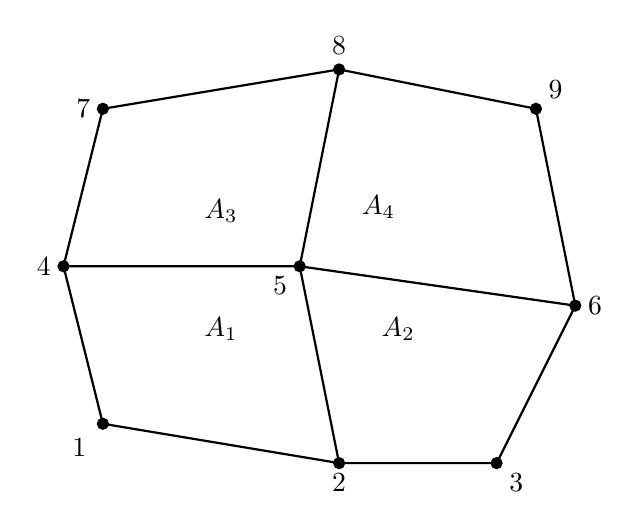
\begin{tikzpicture}
%\draw[fill=gray!5,gray!5](0,0) rectangle (9,7);
%\draw[step=0.5cm,gray,very thin] (0,0) grid (9,7); %background grid
\draw[thick](1.5,1.5) -- (4.5,1) -- (6.5,1) -- (7.5,3) -- (7,5.5) -- (4.5,6) --(1.5,5.5) -- (1,3.5) -- cycle;  
\draw[thick](4.5,1)--(4,3.5)--(4.5,6);
\draw[thick](1,3.5)--(4,3.5)--(7.5,3);
\draw[black,fill=black] (1.5,1.5) circle (2pt); \node[] at (1.2,1.2){1}; %1
\draw[black,fill=black] (4.5,1)   circle (2pt); \node[] at (4.5,0.75){2}; %2
\draw[black,fill=black] (6.5,1)   circle (2pt); \node[] at (6.75,0.75){3}; %3
\draw[black,fill=black] (1,3.5)   circle (2pt); \node[] at (0.75,3.5){4}; %4
\draw[black,fill=black] (4,3.5)   circle (2pt); \node[] at (3.75,3.25){5}; %5
\draw[black,fill=black] (7.5,3)   circle (2pt); \node[] at (7.75,3){6}; %6
\draw[black,fill=black] (1.5,5.5) circle (2pt); \node[] at (1.25,5.5){7}; %7
\draw[black,fill=black] (4.5,6)   circle (2pt); \node[] at (4.5,6.3){8}; %8
\draw[black,fill=black] (7,5.5)   circle (2pt); \node[] at (7.25,5.75){9}; %9
%\draw[thin,dashed](1,3.5)--(4.5,1)--(7.5,3)--(4.5,6)--cycle;
\node[] at (3,2.7){$A_1$}; %8
\node[] at (5.25,2.7){$A_2$}; %8
\node[] at (5,4.25){$A_4$}; %8
\node[] at (3,4.2){$A_3$}; %8
\end{tikzpicture}
\end{center}
\[
q_5^{(1)} = \frac{1}{4}\sum_{e=1}^4 p_e
\] 

In the codes which rely on the $Q_1 \times P_0$ element, the (elemental) pressure
is simply defined as 
\begin{lstlisting}
p=np.zeros(nel,dtype=np.float64)  
\end{lstlisting}
while the nodal pressure is then defined as\footnote{In virtually all stones $p$
stands for the 'raw' pressure and $q$ stands for its projection onto the velocity mesh.} 
\begin{lstlisting}
q=np.zeros(nnp,dtype=np.float64)  
\end{lstlisting}
The element-to-node algorithm is then simply (in 2D):

\begin{lstlisting}
count=np.zeros(nnp,dtype=np.int32)  
for iel in range(0,nel):
    q[icon[0,iel]]+=p[iel]
    q[icon[1,iel]]+=p[iel]
    q[icon[2,iel]]+=p[iel]
    q[icon[3,iel]]+=p[iel]
    count[icon[0,iel]]+=1
    count[icon[1,iel]]+=1
    count[icon[2,iel]]+=1
    count[icon[3,iel]]+=1
q=q/count
\end{lstlisting}



%----------------------------------------------------------------------
\paragraph{Schemes 2,3}.

{\sl Schemes 2,3} are very similar and are presented in Sani \etal (1981) \cite{sagl81a,sagl81b}.
Scheme 2 uses the areas of the surrounding elements as weights for the arithmetic averaging
while scheme 3 uses the area of the triangles:

\begin{multicols}{2}

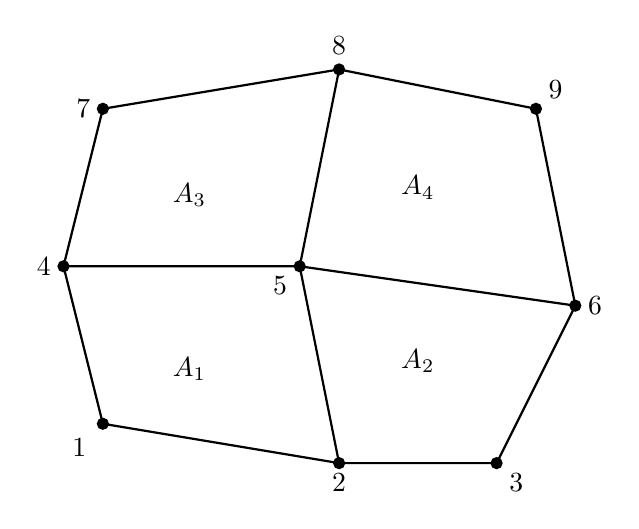
\begin{tikzpicture}
%\draw[fill=gray!5,gray!5](0,0) rectangle (9,7);
%\draw[step=0.5cm,gray,very thin] (0,0) grid (9,7); %background grid
\draw[thick](1.5,1.5) -- (4.5,1) -- (6.5,1) -- (7.5,3) -- (7,5.5) -- (4.5,6) --(1.5,5.5) -- (1,3.5) -- cycle;  
\draw[thick](4.5,1)--(4,3.5)--(4.5,6);
\draw[thick](1,3.5)--(4,3.5)--(7.5,3);
\draw[black,fill=black] (1.5,1.5) circle (2pt); \node[] at (1.2,1.2){1}; %1
\draw[black,fill=black] (4.5,1)   circle (2pt); \node[] at (4.5,0.75){2}; %2
\draw[black,fill=black] (6.5,1)   circle (2pt); \node[] at (6.75,0.75){3}; %3
\draw[black,fill=black] (1,3.5)   circle (2pt); \node[] at (0.75,3.5){4}; %4
\draw[black,fill=black] (4,3.5)   circle (2pt); \node[] at (3.75,3.25){5}; %5
\draw[black,fill=black] (7.5,3)   circle (2pt); \node[] at (7.75,3){6}; %6
\draw[black,fill=black] (1.5,5.5) circle (2pt); \node[] at (1.25,5.5){7}; %7
\draw[black,fill=black] (4.5,6)   circle (2pt); \node[] at (4.5,6.3){8}; %8
\draw[black,fill=black] (7,5.5)   circle (2pt); \node[] at (7.25,5.75){9}; %9
\node[] at (2.6,2.2){$A_1$}; %8
\node[] at (5.5,2.3){$A_2$}; %8
\node[] at (2.6,4.4){$A_3$}; %8
\node[] at (5.5,4.5){$A_4$}; %8
\end{tikzpicture}

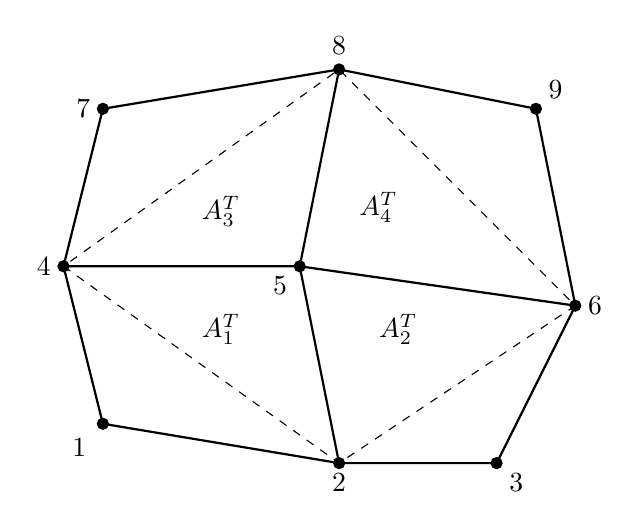
\begin{tikzpicture}
%\draw[fill=gray!5,gray!5](0,0) rectangle (9,7);
%\draw[step=0.5cm,gray,very thin] (0,0) grid (9,7); %background grid
\draw[thick](1.5,1.5) -- (4.5,1) -- (6.5,1) -- (7.5,3) -- (7,5.5) -- (4.5,6) --(1.5,5.5) -- (1,3.5) -- cycle;  
\draw[thick](4.5,1)--(4,3.5)--(4.5,6);
\draw[thick](1,3.5)--(4,3.5)--(7.5,3);
\draw[black,fill=black] (1.5,1.5) circle (2pt); \node[] at (1.2,1.2){1}; %1
\draw[black,fill=black] (4.5,1)   circle (2pt); \node[] at (4.5,0.75){2}; %2
\draw[black,fill=black] (6.5,1)   circle (2pt); \node[] at (6.75,0.75){3}; %3
\draw[black,fill=black] (1,3.5)   circle (2pt); \node[] at (0.75,3.5){4}; %4
\draw[black,fill=black] (4,3.5)   circle (2pt); \node[] at (3.75,3.25){5}; %5
\draw[black,fill=black] (7.5,3)   circle (2pt); \node[] at (7.75,3){6}; %6
\draw[black,fill=black] (1.5,5.5) circle (2pt); \node[] at (1.25,5.5){7}; %7
\draw[black,fill=black] (4.5,6)   circle (2pt); \node[] at (4.5,6.3){8}; %8
\draw[black,fill=black] (7,5.5)   circle (2pt); \node[] at (7.25,5.75){9}; %9
\draw[thin,dashed](1,3.5)--(4.5,1)--(7.5,3)--(4.5,6)--cycle;
\node[] at (3,2.7){$A_1^T$}; %8
\node[] at (5.25,2.7){$A_2^T$}; %8
\node[] at (5,4.25){$A_4^T$}; %8
\node[] at (3,4.2){$A_3^T$}; %8
\end{tikzpicture}

\end{multicols}




\[
q_5^{(2)} = \frac{\sum\limits_{e=1}^4 A_e p_e}{\sum\limits_{e=1}^4 A_e}
\qquad
\qquad
q_5^{(3)} = \frac{\sum\limits_{e=1}^4 A_e^T p_e}{\sum\limits_{e=1}^4 A_e^T}
\] 


\begin{remark} Although Schemes 1,2,3 are similar, scheme 1 is the simplest and fastest
to implement since the areas of neighbouring elements/triangles are not needed.
\end{remark}

\begin{remark} 
Schemes 1,2,3 are identical if all elements are rectangles of identical dimensions.
\end{remark}




%----------------------------------------------------------------------
\paragraph{Scheme 4} This scheme has been designed by me. 
It resembles the last three ones, but the weighing is in this case different.

Let us consider a 1D problem:
\begin{center}
\includegraphics[width=0.5\linewidth]{images/pressure_smoothing/newalgo.png}
\end{center}

Elemental pressures $p_1$ and $p_2$ corresponding to elements 1 and 2 respectively are known at
locations $x_1$ and $x_2$. The two elements have a different size, characterised in this case
by the distances $d_1$ and $d_2$ to their common edge.

The equation of the line passing through points $(x_1,p_1)$ and $(x_2,p_2)$ is 
\[
p(x)=\frac{p_2-p_1}{x_2-x_1}(x-x_1)+p_1
\]
The $x$ coordinate of the common edge is given by $x=x_1+d_1/2$, 
and since $x_2-x_1=(d_1+d_2)/2$, the 
pressure at this location writes:
\[
p(x_M)= \frac{p_2-p_1}{d_1+d_2}d_1+p_1 = \frac{\frac{p_1}{d_1} + \frac{p_2}{d_2}}{\frac{1}{d_1} + \frac{1}{d_2}}
\]
Extrapolating this formula to 2D, $d_1$ and $d_2$ are in fact the element volumes, so that
\[
q_5^{(4)} = 
\frac{\sum\limits_{j=1}^4 \frac{p_j^e}{A_j^e}}{\sum\limits_{j=1}^4 \frac{1}{A_j^e}}
=
\frac{
\frac{p_1^e}{A_1^e}+
\frac{p_2^e}{A_2^e}+
\frac{p_3^e}{A_3^e}+
\frac{p_4^e}{A_4^e}
}{
\frac{1}{A_1^e}+
\frac{1}{A_2^e}+
\frac{1}{A_3^e}+
\frac{1}{A_4^e}
}\]

There remains a problem, due to the presence of the boundary nodes for which 
the sums present in the above equation do not run up to 4. A boundary
node only has three neighbours and a corner node only two. Additional measures
are required for these nodes. 

\begin{center}
\includegraphics[width=0.5\linewidth]{images/pressure_smoothing/newalgo_corner.png}
\end{center}

The pressure value $p_N$ is obtained as follows:
\[
q_N = \frac{ 
 \frac{p_2^e}   {A_2^e}
+\frac{p_3^e}   {A_3^e}
+\frac{p_{2'}^e}{A_{2'}^e}
+\frac{p_{3'}^e}{A_{3'}^e}
}{
 \frac{1}{A_2^e}
+\frac{1}{A_3^e}
+\frac{1}{A_{2'}^e}
+\frac{1}{A_{3'}^e}
}
\]
The areas and pressures of the mirrored elements 2' and 3' are extrapolated from the areas of elements 2 and 6, and 3 and 7 respectively. 
Likewise the pressure $p_M$ at the corner node is obtained through the pressures of its surrounding elements.


%------------------------------------------------------------------------------
\paragraph{Scheme 5 - Least squares} This scheme is presented (among other places) in Lee \etal (1979)
\cite{legs79}. 
Let us start from the patch of 4 $Q_1$ elements counting 9 nodes: 

\begin{center}
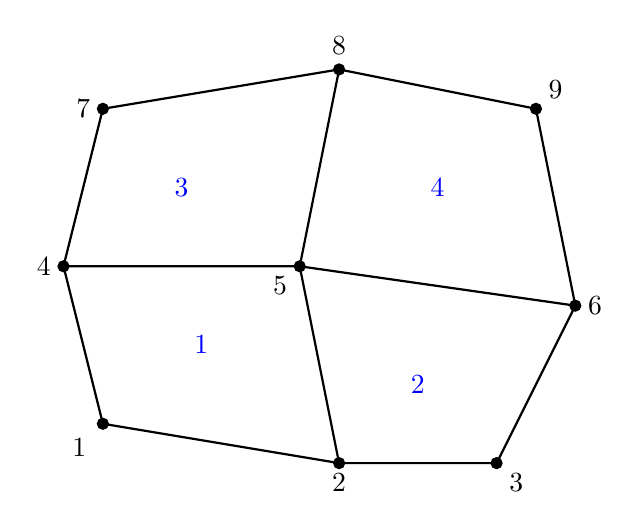
\begin{tikzpicture}
%\draw[fill=gray!5,gray!5](0,0) rectangle (9,7);
%\draw[step=0.5cm,gray,very thin] (0,0) grid (9,7); %background grid
\draw[thick](1.5,1.5) -- (4.5,1) -- (6.5,1) -- (7.5,3) -- (7,5.5) -- (4.5,6) --(1.5,5.5) -- (1,3.5) -- cycle;  
\draw[thick](4.5,1)--(4,3.5)--(4.5,6);
\draw[thick](1,3.5)--(4,3.5)--(7.5,3);

\node[] at (2.75,2.5) {\color{blue}1};
\node[] at (5.5,2) {\color{blue}2};
\node[] at (2.5,4.5) {\color{blue}3};
\node[] at (5.75,4.5) {\color{blue}4};

\draw[black,fill=black] (1.5,1.5) circle (2pt); \node[] at (1.2,1.2){1}; %1
\draw[black,fill=black] (4.5,1)   circle (2pt); \node[] at (4.5,0.75){2}; %2
\draw[black,fill=black] (6.5,1)   circle (2pt); \node[] at (6.75,0.75){3}; %3
\draw[black,fill=black] (1,3.5)   circle (2pt); \node[] at (0.75,3.5){4}; %4
\draw[black,fill=black] (4,3.5)   circle (2pt); \node[] at (3.75,3.25){5}; %5
\draw[black,fill=black] (7.5,3)   circle (2pt); \node[] at (7.75,3){6}; %6
\draw[black,fill=black] (1.5,5.5) circle (2pt); \node[] at (1.25,5.5){7}; %7
\draw[black,fill=black] (4.5,6)   circle (2pt); \node[] at (4.5,6.3){8}; %8
\draw[black,fill=black] (7,5.5)   circle (2pt); \node[] at (7.25,5.75){9}; %9

\end{tikzpicture}
\end{center}



We are looking for a field $q$ living on the nodes.
We build the quantity
\[
J=\iint_\Omega (q-p)^2 dV
\]
where $p$ is the elemental field. To make things clearer we split the integral into 
the sum of elemental integrals:
\[
J=
\iint_{\Omega_1} (q(x,y)-p_1)^2 dV+
\iint_{\Omega_2} (q(x,y)-p_2)^2 dV+
\iint_{\Omega_3} (q(x,y)-p_3)^2 dV+
\iint_{\Omega_4} (q(x,y)-p_4)^2 dV
\]
Inside each element the field $q(x,y)$ is given by a bilinear interpolation so that:
\begin{eqnarray}
J
&=& \iint_{\Omega_1} (\bN_1(x,y) q_1 + \bN_2(x,y)q_2 + \bN_5(x,y)q_5 + \bN_4(x,y)q_4 -p_1)^2 dV \nn\\
&+& \iint_{\Omega_2} (\bN_2(x,y) q_2 + \bN_3(x,y)q_3 + \bN_6(x,y)q_6 + \bN_5(x,y)q_5 -p_2)^2 dV \nn\\
&+& \iint_{\Omega_3} (\bN_4(x,y) q_4 + \bN_5(x,y)q_5 + \bN_8(x,y)q_8 + \bN_7(x,y)q_7 -p_3)^2 dV \nn\\
&+& \iint_{\Omega_4} (\bN_5(x,y) q_5 + \bN_6(x,y)q_6 + \bN_9(x,y)q_9 + \bN_8(x,y)q_8 -p_4)^2 dV 
\end{eqnarray}
where the $N_i$ functions are the basis functions (unusually expressed in $x,y$ coordinates).
The least square procedure looks for the set of $q_i$ such that 
\[
\frac{\partial J}{\partial q_i} =0 \qquad \forall i=1,...9
\]
and this yields 9 equations/constraints for 9 unknowns.
\begin{eqnarray}
\frac{\partial J}{\partial q_1} 
&=& \iint_{\Omega_1} 2 (\bN_1(x,y) q_1 + \bN_2(x,y)q_2 + \bN_5(x,y)q_5 + \bN_4(x,y)q_4 -p_1) \bN_1(x,y) dV \nn\\
\frac{\partial J}{\partial q_2}
&=& \iint_{\Omega_1} 2(\bN_1(x,y) q_1 + \bN_2(x,y)q_2 + \bN_5(x,y)q_5 + \bN_4(x,y)q_4 -p_1) \bN_2(x,y) dV \nn\\
&+& \iint_{\Omega_2} 2(\bN_2(x,y) q_2 + \bN_3(x,y)q_3 + \bN_6(x,y)q_6 + \bN_5(x,y)q_5 -p_2) \bN_2(x,y) dV \nn\\
\frac{\partial J}{\partial q_3}
&=& \iint_{\Omega_2} 2(\bN_2(x,y) q_2 + \bN_3(x,y)q_3 + \bN_6(x,y)q_6 + \bN_5(x,y)q_5 -p_2) \bN_3(x,y) dV \nn\\
\frac{\partial J}{\partial q_4}
&=& \iint_{\Omega_1} 2(\bN_1(x,y) q_1 + \bN_2(x,y)q_2 + \bN_5(x,y)q_5 + \bN_4(x,y)q_4 -p_1) \bN_4(x,y) dV \nn\\
&+& \iint_{\Omega_3} 2(\bN_4(x,y) q_4 + \bN_5(x,y)q_5 + \bN_8(x,y)q_8 + \bN_7(x,y)q_7 -p_3) \bN_4(x,y) dV \nn\\
\frac{\partial J}{\partial q_5}
&=& \iint_{\Omega_1} 2(\bN_1(x,y) q_1 + \bN_2(x,y)q_2 + \bN_5(x,y)q_5 + \bN_4(x,y)q_4 -p_1) \bN_5(x,y) dV \nn\\
&+& \iint_{\Omega_2} 2(\bN_2(x,y) q_2 + \bN_3(x,y)q_3 + \bN_6(x,y)q_6 + \bN_5(x,y)q_5 -p_2) \bN_5(x,y) dV \nn\\
&+& \iint_{\Omega_3} 2(\bN_4(x,y) q_4 + \bN_5(x,y)q_5 + \bN_8(x,y)q_8 + \bN_7(x,y)q_7 -p_3) \bN_5(x,y) dV \nn\\
&+& \iint_{\Omega_4} 2(\bN_5(x,y) q_5 + \bN_6(x,y)q_6 + \bN_9(x,y)q_9 + \bN_8(x,y)q_8 -p_4) \bN_5(x,y) dV \nn\\
\frac{\partial J}{\partial q_6}
&=& \iint_{\Omega_2} 2(\bN_2(x,y) q_2 + \bN_3(x,y)q_3 + \bN_6(x,y)q_6 + \bN_5(x,y)q_5 -p_2) \bN_6(x,y) dV \nn\\
&+& \iint_{\Omega_4} 2(\bN_5(x,y) q_5 + \bN_6(x,y)q_6 + \bN_9(x,y)q_9 + \bN_8(x,y)q_8 -p_4) \bN_6(x,y) dV \nn\\
\frac{\partial J}{\partial q_7}
&=& \iint_{\Omega_3} 2(\bN_4(x,y) q_4 + \bN_5(x,y)q_5 + \bN_8(x,y)q_8 + \bN_7(x,y)q_7 -p_3) \bN_7(x,y) dV \nn\\
\frac{\partial J}{\partial q_8}
&=& \iint_{\Omega_3} 2(\bN_4(x,y) q_4 + \bN_5(x,y)q_5 + \bN_8(x,y)q_8 + \bN_7(x,y)q_7 -p_3) \bN_8(x,y)dV \nn\\
&+& \iint_{\Omega_4} 2(\bN_5(x,y) q_5 + \bN_6(x,y)q_6 + \bN_9(x,y)q_9 + \bN_8(x,y)q_8 -p_4) \bN_8(x,y)dV \nn\\ 
\frac{\partial J}{\partial q_9}
&=& \iint_{\Omega_4} 2(\bN_5(x,y) q_5 + \bN_6(x,y)q_6 + \bN_9(x,y)q_9 + \bN_8(x,y)q_8 -p_4) \bN_9(x,y)dV 
\end{eqnarray}
The factor 2 are removed and the terms $\int p_i N_j $ are known so they end up in the right hand side.
\begin{eqnarray}
 \iint_{\Omega_1} (\bN_1 \bN_1 q_1 + \bN_1 \bN_2 q_2 + \bN_1 \bN_5 q_5 + \bN_1 \bN_4 q_4) dV 
&=& \iint_{\Omega_1} p_1 N_1 dV \nn\\
 \iint_{\Omega_1} (\bN_2 \bN_1 q_1 + \bN_2 \bN_2 q_2 + \bN_2 \bN_5 q_5 + \bN_2 \bN_4 q_4) dV \nn\\
+\iint_{\Omega_2} (\bN_2 \bN_2 q_2 + \bN_3 \bN_2 q_3 + \bN_6 \bN_2 q_6 + \bN_5 \bN_2 q_5) dV 
&=& \iint_{\Omega_1} p_1N_2 dV + \iint_{\Omega_2}  p_2 \bN_2 dV \nn\\
\nn\\
\dots &=& \dots \nn\\
\nn\\
 \iint_{\Omega_4} (\bN_9\bN_5 q_5 + \bN_9\bN_6q_6 + \bN_9\bN_9q_9 + \bN_9\bN_8q_8) dV &=&  \iint_{\Omega_4} p_4 \bN_9 dV 
\end{eqnarray}

The mass matrices corresponding to the four elements are 
\[
{\bm M}_1 = \int_{\Omega_1} \left( \begin{array}{cccc}
 \bN_1 \bN_1 & \bN_1 \bN_2 & \bN_1 \bN_5 & \bN_1 \bN_4 \\
 \bN_2 \bN_1 & \bN_2 \bN_2 & \bN_2 \bN_5 & \bN_2 \bN_4 \\
 \bN_5 \bN_1 & \bN_5 \bN_2 & \bN_5 \bN_5 & \bN_5 \bN_4 \\
 \bN_4 \bN_1 & \bN_4 \bN_2 & \bN_4 \bN_5 & \bN_4 \bN_4 
\end{array}\right) dV
\qquad
{\bm M}_2 = \int_{\Omega_2} \left( \begin{array}{cccc}
 \bN_2 \bN_2 & \bN_2 \bN_3 & \bN_2 \bN_6 & \bN_2 \bN_5 \\
 \bN_3 \bN_2 & \bN_3 \bN_3 & \bN_3 \bN_6 & \bN_3 \bN_5 \\
 \bN_6 \bN_2 & \bN_6 \bN_3 & \bN_6 \bN_6 & \bN_6 \bN_5 \\
 \bN_5 \bN_2 & \bN_5 \bN_3 & \bN_5 \bN_6 & \bN_5 \bN_5 
\end{array}\right) dV
\]
\[
{\bm M}_3 = \int_{\Omega_3} \left( \begin{array}{cccc}
 \bN_4 \bN_4 & \bN_4 \bN_5 & \bN_4 \bN_8 & \bN_4 \bN_7 \\
 \bN_5 \bN_4 & \bN_5 \bN_5 & \bN_5 \bN_8 & \bN_5 \bN_7 \\
 \bN_8 \bN_4 & \bN_8 \bN_5 & \bN_8 \bN_8 & \bN_8 \bN_7 \\
 \bN_7 \bN_4 & \bN_7 \bN_5 & \bN_7 \bN_8 & \bN_7 \bN_7 
\end{array}\right) dV
\qquad
{\bm M}_4 = \int_{\Omega_4} \left( \begin{array}{cccc}
 \bN_5 \bN_5 & \bN_5 \bN_6 & \bN_5 \bN_9 & \bN_5 \bN_8 \\
 \bN_6 \bN_5 & \bN_6 \bN_6 & \bN_6 \bN_9 & \bN_6 \bN_8 \\
 \bN_9 \bN_5 & \bN_9 \bN_6 & \bN_9 \bN_9 & \bN_9 \bN_8 \\
 \bN_8 \bN_5 & \bN_8 \bN_6 & \bN_8 \bN_9 & \bN_8 \bN_8 
\end{array}\right) dV
\]
so that the 9 equations above are actually the result of the assembly process of these four 
elemental systems:
\[
\left( \iint_{\Omega_e} \vec{\bN}^T\vec{\bN} dV \right) \cdot \vec{q}_e = \iint_{\Omega_i} \vec{\bN}^T p_e dV 
\qquad\qquad e=1,2,3,4
\]


%------------------------------------------------------------------------------
\paragraph{Scheme 6 - Consistent pressure recovery}

The is the method presented in Zienkiewicz \& Nakazawa (1982) \cite{zina82}. In the second part 
of this publication the authors wish to establish a simple and effective numerical method to calculate 
variables eliminated by the penalisation process. 
The method involves an additional finite element solution for the nodal pressures using 
the same finite element basis and numerical quadrature as used for the velocity.

Let us start with\footnote{I here voluntarily use $q$ instead of $p$}:
\[
q = -\lambda \vec\nabla\cdot \vec\upnu
\]
We are going to treat this equation as any other PDE in the context of the FE method, i.e. 
we are going to establish its weak form. 
We assume that the pressure is given inside an element by
\[
q(x,y) = \sum_{i=1}^4 \bN_i(x,y) q_i = \vec{\bN} \cdot \vec{q}
\]
and the velocity:
\[
\vec\upnu = (u,v) 
\qquad 
\qquad 
u(x,y)  = \sum_{i=1}^4 \bN_i(x,y) u_i
\qquad 
\qquad 
v(x,y)  = \sum_{i=1}^4 \bN_i(x,y) v_i
\]
where the $\bN_i$ are the $Q_1$ basis functions and $q_i$ are the sought after nodal values. 
We multiply the equation above by a $Q_1$ basis function $\bN_i$ and integrate over the whole domain:
\[
\iint_\Omega \bN_i(x,y) q(x,y) \; dxdy 
= -\lambda \iint_\Omega \bN_i \vec\nabla\cdot \vec\upnu  \; dx dy
\]
As before we now focus on the above expression inside a single element $e$:
\[
\iint_{\Omega_e} \bN_i(x,y) q(x,y) \; dxdy = -\lambda \iint_{\Omega_e} \bN_i \vec\nabla\cdot \vec\upnu \; dx dy
\]
After $\bN_i \rightarrow \vec{\bN}=(\bN_1,\bN_2,\bN_3,\bN_4)^T$, the left hand side term becomes:
\[
\iint _{\Omega_e} \vec{\bN}^T q(x,y) \; dxdy 
=
\iint _{\Omega_e} \vec{\bN}^T \vec{\bN} \cdot \vec{q} \; dxdy 
=
\left(\underbrace{\iint _{\Omega_e} \vec{\bN}^T \vec{\bN} dxdy}_{{\bm M}_e} \right) \cdot \vec{q}  
\]
where ${\bm M}_e$ is the elemental mass matrix.
We now turn to the right hand side. We have
\[
\vec\nabla\cdot \vec\upnu
= \frac{\partial u}{\partial x}+\frac{\partial v}{\partial y}
= \sum_i \frac{\partial \bN_i}{\partial x} u_i + \sum_i \frac{\partial \bN_i}{\partial y} v_i 
\]
We here too define $\vec{V}_e=(u_1,v_1,u_2,v_2,u_3,v_3,u_4,v_4)^T$ so that 

\begin{eqnarray}
&& \iint_{\Omega_e} \vec{\bN} {\vec \nabla}\cdot {\vec \upnu} \; dV \nn\\
&=& \iint_{\Omega_e} \vec{\bN}^T \sum_{i=1}^{4} 
\left( \frac{\partial \bN_i}{\partial x} u_i + \frac{\partial \bN_i}{\partial y} v_i 
\right)  
dV \nonumber\\
&=& 
\iint_{\Omega_e} 
\left(
\begin{array}{c}
\bN_1 \left(
\sum\limits_{i=1}^{4} \frac{\partial \bN_i}{\partial x} u_i +
\sum\limits_{i=1}^{4} \frac{\partial \bN_i}{\partial y} v_i \right) \\
\bN_2 \left(
\sum\limits_{i=1}^{4} \frac{\partial \bN_i}{\partial x} u_i +
\sum\limits_{i=1}^{4} \frac{\partial \bN_i}{\partial y} v_i \right) \\
\bN_3 \left(
\sum\limits_{i=1}^{4} \frac{\partial \bN_i}{\partial x} u_i +
\sum\limits_{i=1}^{4} \frac{\partial \bN_i}{\partial y} v_i \right) \\
\bN_4 \left(
\sum\limits_{i=1}^{4} \frac{\partial \bN_i}{\partial x} u_i +
\sum\limits_{i=1}^{4} \frac{\partial \bN_i}{\partial y} v_i \right) 
\end{array}
\right) dV \nonumber \\  %%%%%%%%%%%%%%%%%%%%%%%%%%
&=& 
\int_{\Omega_e} 
\left(
\begin{array}{ccc}
{\bN}_1& {\bN}_1 &  0 \\\\
{\bN}_2& {\bN}_2 &  0 \\\\
{\bN}_3& {\bN}_3 &  0 \\\\
{\bN}_4& {\bN}_4 &  0 
\end{array}
\right)
\cdot
\left(
\begin{array}{c}
\sum\limits_i \frac{\partial \bN_i}{\partial x} u_i \\ \\
\sum\limits_i \frac{\partial \bN_i}{\partial y} v_i \\ \\
\sum\limits_i (\frac{\partial \bN_i}{\partial y} u_i\! +\! \frac{\partial \bN_i}{\partial x} v_i) 
\end{array}
\right)
\; dV \nonumber\\ %%%%%%%%%%%%%%%%%%%%%%%%%%
&=& 
\int_{\Omega_e} 
\underbrace{
\left(
\begin{array}{cccccc}
{\bN}_1 & {\bN}_1 &  0 \\
{\bN}_2 & {\bN}_2 &  0 \\
{\bN}_3 & {\bN}_3 &  0 \\
{\bN}_4 & {\bN}_4 &  0 
\end{array}
\right)
}_{{\bm N}}
\cdot
\underbrace{
\left(\begin{array}{cccccccc}
\partial_x \bN_1 & 0 &  
\partial_x \bN_2 & 0 &  
\partial_x \bN_3 & 0 &  
\partial_x \bN_4 & 0 \\ \\
0 & \partial_y \bN_1 &   
0 & \partial_y \bN_2 &   
0 & \partial_y \bN_3 &   
0 & \partial_y \bN_4 \\ \\
\partial_y \bN_1 & \partial_x \bN_1 &  
\partial_y \bN_2 & \partial_x \bN_2 &  
\partial_y \bN_3 & \partial_x \bN_3 &  
\partial_y \bN_4 & \partial_x \bN_4 
\end{array}\right)}_{{\bm B}}
\cdot \vec{V}_e
\; dV  \nonumber \\
&=& 
\left(\int_{\Omega_e} {\bm N} \cdot {\bm B} \; dV \right) \cdot \vec{V}_e \nonumber\\
&=& -\G_e^T \cdot {\vec V}_e
\end{eqnarray}

After assembly we arrive at
\[
{\bm M} \cdot \vec{q} = \lambda \G^T \cdot {\vec V} 
\qquad
\text{with}
\qquad
\G_e = -\int_{\Omega_e} {\bm N} \cdot {\bm B} \; dV
\]
where ${\bm M}$ is the global mass matrix, $\vec{q}$ the vector of all 
nodal pressures, $\G$ the discrete gradient matrix and $\vec{V}$
the (velocity) solution vector. 
The system can be easily solved since the mass matrix is a friendly matrix.
The vector ${\vec q}$ contains the nodal pressure values directly, with 
no need for a smoothing scheme! 

\begin{remark}
Very importantly, the mass matrix ${\bm M}$ is to be evaluated at the full integration points, 
while the constraint part (the right hand side of the equation) is to be evaluated at 
the reduced integration point, i.e. in the middle of the element.  
\end{remark}

\begin{remark}
As noted in \cite{zina82}, it is interesting to note that when linear elements are used 
and the lumped matrices are used for the ${\bm M}$ the resulting algebraic equation is identical 
to the smoothing scheme 1 only if a uniform square finite element 
mesh is used. In this respect this method is expected to yield different results when elements 
are not square or even rectangular.
\end{remark}

\begin{remark}
The third column of the matrix ${\bm N}$
and the last line of the ${\bm B}$ matrix could be removed altogether.
If your code is based on the mixed formulation, then you already 
have built matrix $\G$ so you can easily re-use this piece of code 
to compute $\G$ again, this time with a reduced integration quadrature.
If you are using the penalty formulation then you need to program 
all from scratch and then simply do away with these unnecessary terms, or 
you can direcly build the rhs as $\int_{\Omega_e} \vec{\bN}^T p_e$ (assuming
you have previously computed the pressure in the middle of each element 
by means of $p=-\lambda\vec\nabla\cdot\vec\upnu$).
\end{remark}

\begin{remark}
This  scheme is identical to the least square scheme!
\end{remark}


%--------------------------------------------------------------
\paragraph{Scheme 7}

Same as scheme 6, but with lumped mass matrix.  


%--------------------------------------------------------------
\paragraph{Scheme 8 - bilinear interpolation} Let us assume that the centers of the 
four elements make a $Q_1$ quadrilateral element, as shown on this figure:


\begin{center}
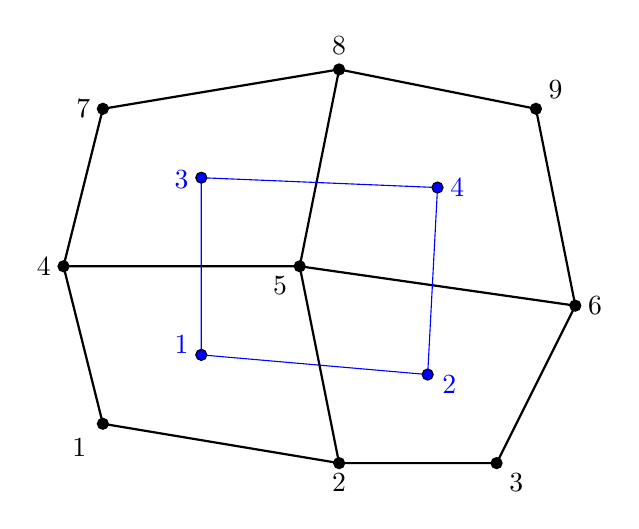
\begin{tikzpicture}
%\draw[fill=gray!5,gray!5](0,0) rectangle (9,7);
%\draw[step=0.5cm,gray,very thin] (0,0) grid (9,7); %background grid
\draw[thick](1.5,1.5) -- (4.5,1) -- (6.5,1) -- (7.5,3) -- (7,5.5) -- (4.5,6) --(1.5,5.5) -- (1,3.5) -- cycle;  
\draw[thick](4.5,1)--(4,3.5)--(4.5,6);
\draw[thick](1,3.5)--(4,3.5)--(7.5,3);

\draw[black,fill=blue] (2.75,2.375) circle (2pt); 
\node[] at (2.5,2.5) {\color{blue}1};
\draw[black,fill=blue] (5.625,2.125) circle (2pt); 
\node[] at (5.9,2) {\color{blue}2};
\draw[black,fill=blue] (5.75,4.5) circle (2pt); 
\node[] at (2.5,4.6) {\color{blue}3};
\draw[black,fill=blue] (2.75,4.625) circle (2pt); 
\node[] at (6,4.5) {\color{blue}4};

\draw[black,fill=black] (1.5,1.5) circle (2pt); \node[] at (1.2,1.2){1}; %1
\draw[black,fill=black] (4.5,1)   circle (2pt); \node[] at (4.5,0.75){2}; %2
\draw[black,fill=black] (6.5,1)   circle (2pt); \node[] at (6.75,0.75){3}; %3
\draw[black,fill=black] (1,3.5)   circle (2pt); \node[] at (0.75,3.5){4}; %4
\draw[black,fill=black] (4,3.5)   circle (2pt); \node[] at (3.75,3.25){5}; %5
\draw[black,fill=black] (7.5,3)   circle (2pt); \node[] at (7.75,3){6}; %6
\draw[black,fill=black] (1.5,5.5) circle (2pt); \node[] at (1.25,5.5){7}; %7
\draw[black,fill=black] (4.5,6)   circle (2pt); \node[] at (4.5,6.3){8}; %8
\draw[black,fill=black] (7,5.5)   circle (2pt); \node[] at (7.25,5.75){9}; %9

\draw[blue](2.75,2.375)--(5.625,2.125)--(5.75,4.5)--(2.75,4.625)--cycle;
\end{tikzpicture}
\end{center}




The values at the corners are $p_1$,
$p_2$, $p_3$ and $p_4$. Assuming that the pressure inside this element can be represented 
by a bilinear field, we have 
\[
p(x,y)= a+ bx +cy +dxy
\]
where the coefficients will be determined by ensuring that $p(x_i,y_i)=p_i$ for $i=1,2,3,4$, or:
\begin{eqnarray}
a+bx_1+cy_1+dx_1y_1 &=& p_1 \\
a+bx_2+cy_2+dx_2y_2 &=& p_2 \\
a+bx_3+cy_3+dx_3y_3 &=& p_3 \\
a+bx_4+cy_4+dx_4y_4 &=& p_4 
\end{eqnarray}
i.e.
\[
\left(
\begin{array}{cccc}
1 & x_1 & y_1 & x_1y_1 \\
1 & x_2 & y_2 & x_2y_2 \\
1 & x_3 & y_3 & x_3y_3 \\
1 & x_4 & y_4 & x_4y_4
\end{array}
\right)\cdot
\left(
\begin{array}{c}
a \\b\\c\\d
\end{array}
\right)
=
\left(
\begin{array}{c}
p_1\\p_2\\p_3\\p_4
\end{array}
\right)
\]

There remains an issue with nodes which are on the boundaries of the domain. These are of course not 
'surrounded' by four pressure values so the above algorithm does not apply directly. However, looking 
at the above figure, and assuming that node 1 is a lower left corner of a 2D domain, we can use the 
bilinear interpolation based on elements 1,2,3,4 to extrapolate a nodal pressure value at node 1. 
The same would apply for nodes 2 and 4 for example. 

\begin{remark}
This scheme is not applicable to quadtree-based meshed.
\end{remark}





\newpage %-----------------------------------------------------------------------------------------
\subsection{Pressure scaling} \index{general}{pressure scaling}
\begin{flushright} {\tiny {\color{gray} pressure\_scaling.tex}} \end{flushright}
%~~~~~~~~~~~~~~~~~~~~~~~~~~~~~~~~~~~~~~~~~~~~~~~~~~~~~~~~~~~~~~~~~~~~~~~~~~~~~~~~~~~~~~~~~~~~~~~~~~

As nicely explained in the 
step 32 of deal.ii\footnote{\url{https://www.dealii.org/9.0.0/doxygen/deal.II/step\_32.html}},
we often need to scale the $\G$ block since it is many orders of magnitude smaller than $\K$ (especially in geodynamics where viscosities are $\sim 10^{22}$), 
which introduces large inaccuracies in the solving process to the point that the solution is nonsensical. 
This scaling coefficient is $\eta/L$ where $\eta$ and $L$ are representative viscosities and lengths. 
We start from 
\[
\left(
\begin{array}{cc}
\K & \G \\ \G^T & -\C 
\end{array}
\right)
\cdot
\left(
\begin{array}{c}
\vec{\cal V} \\ \vec{\cal P}
\end{array}
\right)
=
\left(
\begin{array}{c}
\vec{f} \\ \vec{h}
\end{array}
\right)
\]
and introduce the scaling coefficient as follows (which in fact does not alter the solution at all):
\[
\left(
\begin{array}{cc}
\K & \frac{\eta}{L}\G \\ \frac{\eta}{L}\G^T & - \frac{\eta^2}{L^2} \C 
\end{array}
\right)
\cdot
\left(
\begin{array}{c}
\vec{\cal V} \\\frac{L}{\eta} \vec{\cal P}
\end{array}
\right)
=
\left(
\begin{array}{c}
 \vec{f} \\ \frac{\eta}{L} \vec{h}
\end{array}
\right)
\]
We then end up with the modified Stokes system:
\[
\left(
\begin{array}{cc}
\K & \underline{\G} \\ \underline{\G}^T & \underline{\C} 
\end{array}
\right)
\cdot
\left(
\begin{array}{c}
\vec{\cal V} \\ \underline{\vec{\cal P}}
\end{array}
\right)
=
\left(
\begin{array}{c}
\vec{f} \\ \underline{\vec{h}}
\end{array}
\right)
\]
where 
\[
\underline{\G}=\frac{\eta}{L}\G
\quad\quad
\quad\quad
\underline{\vec{\cal P}}=\frac{L}{\eta} \vec{\cal P}
\quad\quad
\quad\quad
\underline{\C}=\frac{\eta^2}{L^2} \C
\quad\quad
\quad\quad
\underline{\vec{h}}=\frac{\eta}{L}\vec{h}
\]
After the solve phase, we recover the real pressure with $\vec{\cal P}=\frac{\eta}{L}\underline{\vec{\cal P}}$.

Note that in Section~\ref{sec:block_scaling} we revisit the topic and this time 
scale all the blocks of the Stokes matrix.



 %-------------------------------------------
\newpage %-----------------------------------------------------------------------------------------
\subsection{Pressure normalisation, nullspace\label{ss_pnorm}} 
%..................................................
\subsubsection{Basic idea and naive implementation}

When Dirichlet boundary conditions are imposed everywhere on the boundary, pressure is only present by its gradient in 
the equations. It is thus determined up to an arbitrary constant (one speaks then of a null space of size 1).  
In such a case, one commonly impose the average of the pressure over the whole domain or on a subsect of the boundary 
to be have a zero average, i.e.
\[
\int_\Omega p dV = 0
\]
Another possibility is to impose the pressure value at a single node. 

Let us assume that we are using $Q_1 \times P_0$ elements. Then the pressure is constant 
inside each element. 
The integral above becomes:
\[
\int_\Omega p dV = 
\sum_e  \int_{\Omega_e} p dV = 
\sum_e  p_e \int_{\Omega_e} dV = 
\sum_e  p_e A_e = 0
\]
where the sum runs over all elements $e$ of area $A_e$.
This can be rewritten 
\[
\LLL^T \cdot \vec{\cal P}=0
\] 
and it is a constraint on the pressure solution. 
As we have seen before \ref{XXX}, we can associate to it a 
Lagrange multiplier $\lambda$ so that we must solve the modified Stokes system:
\[
\left(
\begin{array}{ccc}
\K & \G & 0\\ 
\G^T & 0 & \LLL \\
0 & \LLL^T & 0
\end{array}
\right)
\cdot
\left(
\begin{array}{c}
\vec{\cal V} \\ \vec{\cal P} \\ \lambda
\end{array}
\right)
=
\left(
\begin{array}{c}
\vec{f} \\ \vec{h} \\ 0
\end{array}
\right)
\]
When higher order spaces are used for pressure (continuous or discontinuous)
one must then carry out the above integration numerically by means of (usually)
a Gauss-Legendre quadrature.

Although valid, this approach has one main disadvantage: it makes the Stokes matrix larger (although
marginally so -- only one row and column are added), but more importantly it prevents the use of some
of the solving strategies of Section \ref{solvers}.


%..................................................
\subsubsection{Implementation -- the real deal}

The idea is actually quite simple and requires two steps:
\begin{enumerate}
\item remove the null space by prescribing the pressure at one location and solve the system;
\item post-process the pressure so as to arrive at a pressure field which fulfills the required normalisation (surface, volume, ...)
\end{enumerate}

\todo[inline]{finish explain}






 %----
\newpage %-----------------------------------------------------------------------------------------
\subsection{Solving the Stokes system \label{sec:solvers}} \begin{flushright} {\tiny {\color{gray} \tt solvers.tex}} \end{flushright}
%~~~~~~~~~~~~~~~~~~~~~~~~~~~~~~~~~~~~~~~~~~~~~~~~~~~~~~~~~~~~~~~~~~~~~~~~~~~~~~~~~~~~~~~~~~~~~~~~~~

Let us start again from the (full) Stokes system:
\begin{equation}
\underbrace{
\left(
\begin{array}{cc}
\K & \G \\ \G^T & -\C 
\end{array}
\right)
}_{\cal A}
\cdot
\left(
\begin{array}{c}
\vec{\cal V} \\ \vec{\cal P}
\end{array}
\right)
=
\left(
\begin{array}{c}
\vec{f} \\ \vec{h}
\end{array}
\right)
\label{StokesSyst}
\end{equation}
We need to solve this system in order to obtain the solution, i.e. the $\vec{\cal V}$ 
and $\vec{\cal P}$ vectors. But how? 
Unfortunately, this question is not simple to answer and the appropriate method depends on many 
parameters, but mainly on how big the matrix blocks are and what the condition number of the matrix $\K$ is. 

First let us start with an obvious question: couldn't we just compute the inverse of the matrix ${\cal A}$?
Under the assumption that the inverse of $\K$ and $\SSS$ exists, we can and we find\footnote{The matrix 
$\C$ is here omitted but it bears no consequences on the conclusion.}
\[
{\cal A}^{-1} = 
\left(
\begin{array}{cc}
\K & \G \\ \G^T & 0
\end{array}
\right)^{-1}
=
\left(
\begin{array}{cc}
\K^{-1} + \K^{-1} \cdot \G \cdot\SSS^{-1} \cdot\G^T \cdot\K^{-1} & -\K^{-1} \cdot\G \cdot\SSS^{-1} \\ 
-\SSS^{-1} \cdot\G^T \cdot\K^{-1}  &  \SSS^{-1}
\end{array}
\right)
\]
However, such an expression is of limited interest in the numerical solution of saddle
point problems since it showcases 5 times the inverse of $\K$ and more importantly
the inverse of the Schur complement matrix $\SSS$ which is likely to be a full matrix so 
that we never want to compute it explicitely.


As concisely explained in Clevenger \& Heister (2021) \cite{clhe21}, 
there are three common approaches used in the literature for solving the above equation on large scales:
\begin{itemize}
\item a pressure corrected, Schur complement CG scheme, using multigrid as an 
approximation to the velocity block;
\item a block-preconditioned Krylov
method, also using multigrid on the velocity block.
For this method, there are two main types:
\begin{itemize}
\item GMRES\cite{mabl15,rumi15} (or any Krylov method not requiring symmetry) with
block-triangular preconditioner (This is what \aspect does):
\[
{\bm P} = \left(
\begin{array}{cc}
\K & \G \\
0 & - \SSS
\end{array}
\right)
\]

\item MINRES\cite{gmhj16} with block-diagonal preconditioner
\[
{\bm P} = \left(
\begin{array}{cc}
\K & 0 \\
0 & - \SSS
\end{array}
\right)
\]

\end{itemize}

\item an all-at-once multigrid performed on the entire Stokes system, using Uzawa-type smoothers.
\end{itemize}



\Literature: Preconditioners for Incompressible Navier-Stokes Solvers 
\begin{small}
\begin{itemize}
\item \fullcite{benz02}
\item \fullcite{bewa08}
\item \fullcite{urvs08}
\item \fullcite{seuv10}
\item Saddle point preconditioners have been extensively discussed and studied \cite{bewa08}, \cite{dewu04}
\item Diagonal preconditioners in \cite{shrb01}, \cite{babc94}.
\end{itemize}
\end{small}

\Literature: Solving Stokes Saddle Point problem
\begin{small}
\begin{itemize}
\item \fullcite{laqu86}
\item \fullcite{rotf90}
\item \fullcite{frha93}
\item \fullcite{elgo94}
\item \fullcite{cheb96}, \fullcite{elma96}
\item \fullcite{brpv97}
\item \fullcite{lixu01}
\item \fullcite{dogs06}, \fullcite{lica06}
\item \fullcite{hoow17}
\item Pragmatic solvers for 3D Stokes problems with heterogeneous coefficients \cite{samb20}
\end{itemize}
\end{small}



%------------------------------------------------------------------------------
\subsection{Block diagonal scaling} \label{sec:block_scaling}

We have already seen in Section~\ref{pscaling} how and why we scale the $\G$ block. 
We revisit this topic more thoroughly in what follows.
This section is borrowed from Section~2.6 of \textcite{mamo08} (2008).

Let us state again the equation we wish to solve (Eq. 6 in the paper):
\[
\begin{pmatrix}
\K & \G \\
\G^T & 0
\end{pmatrix}
\cdot
\begin{pmatrix}
\vec{\cal V} \\
\vec{\cal P}
\end{pmatrix}
=
\begin{pmatrix}
\vec{f} \\
\vec{h}
\end{pmatrix}
\]

Prior to solving this equation, the autors apply a row/column scaling to the equation
to effectively normalize the operators $\K$ and $\G$ with the intention of
reducing round off errors. The scaling is particularly important for
problems in geodynamics when dimensional quantities are used to
define the problem and because of the large, local variations which
may occur in the constitutive tensor (in practice, the effective viscosity) . 

They apply a symmetric block diagonal scaling to the equation via the scaling matrix\footnote{
The $S$ stands for 'scaling', the Schur complement is given by $\SSS$}
\[
{\bm S} = 
\begin{pmatrix}
{\bm S}_1 & 0 \\ 0 & {\bm S}_2
\end{pmatrix}
\]
Writing the first equation as ${\bm A} \cdot \vec{x} = \vec{b}$, 
the symmetric scaling operation is applied as follows:
\[
{\bm S}^{-1} \cdot {\bm A} \cdot \vec{x}= {\bm S}^{-1} \cdot \vec{b} 
\]
followed by\footnote{${\bm S}^{-T}$ is the inverse of the transpose of the matrix.} 
\[
{\bm S}^{-1} \cdot {\bm A} \cdot {\bm S}^{-T} \cdot {\bm S}^T \cdot \vec{x}= {\bm S}^{-1} \cdot \vec{b} 
\]
to give the scaled system ${\bm A}_s \cdot \vec{y}_s = \vec{b}_s$ , where the operator 
${\bm A}_s$ is given by
\begin{eqnarray}
{\bm S}^{-1} \cdot {\bm A} \cdot {\bm S}^{-T} 
&=&\begin{pmatrix}
{\bm S}_1^{-1} & 0 \\ 0 & {\bm S}_2^{-1}
\end{pmatrix}
\cdot 
\begin{pmatrix}
\K & \G \\
\G^T & 0
\end{pmatrix}
\cdot
\begin{pmatrix}
{\bm S}_1^{-T} & 0 \\ 0 & {\bm S}_2^{-T}
\end{pmatrix} \nn\\
&=&
\begin{pmatrix}
{\bm S}_1^{-1} \cdot \K \cdot {\bm S}_1^{-T} & {\bm S}_1^{-1} \cdot \G \cdot {\bm S}_2^{-T} \\
({\bm S}_1^{-1} \cdot \G \cdot {\bm S}_2^{-T})^{T} & 0 
\end{pmatrix} \nn\\
&=&
\begin{pmatrix}
\K_s & \G_s \\
\G^T_s & 0
\end{pmatrix} \nn\\
&=&{\bm A}_s \nn
\end{eqnarray}
with
\[
{\bm S}^T \cdot \vec{x} 
= 
\begin{pmatrix}
{\bm S}_1^T \cdot \vec{\cal V} \\
{\bm S}_2^T \cdot \vec{\cal P}
\end{pmatrix}
=\vec{y}_s
\qquad\qquad
{\bm S}^{-1} \cdot \vec{b} = 
\begin{pmatrix}
{\bm S}_1^{-1}\cdot\vec{f} \\
{\bm S}_2^{-1}\cdot\vec{h}
\end{pmatrix}
=\vec{b}_s
\]
Following the solution of the scaled system, we recover the un-scaled
solution from $\vec{x} = {\bm S}^{-T} \cdot  \vec{y}_s$. 
The form of the scaling operation is based
on the preconditioner described in Rusten and Winther (1992). For
the purpose of scaling, rather than full preconditioning of the indefinite system, 
we let both ${\bm S}_1$ and ${\bm S}_2$ be diagonal matrices. We seek
to approximately normalize the operators $\K$ and $\G$.

Thus we let 
\[
S_1(i,i) = \sqrt{ \max_j K_{ij}} \qquad \forall i \in [1,NfemV]
\]
The choice for ${\bm S}_2$ is based on the requirement that $\G^T_s\cdot \G_s \simeq {\bm 1}_{Nfemp}$ (i.e.
the identity matrix of size $NfemP\times NfemP$) which yields the relation
\[
\G^T_s \cdot \G = ({\bm S}_1^{-1} \cdot \G \cdot {\bm S}_2^{-T})^T 
\cdot ({\bm S}_1^{-1} \cdot \G \cdot {\bm S}_2^{-T} )
= {\bm S}_2^{-1} \cdot \G^T \cdot {\bm S}_1^{-T} \cdot {\bm S}_1^{-1} \cdot \G \cdot {\bm S}_2^{-T} = {\bm 1}
\]
We can left multiply by ${\bm S}_2$ and right multiply by  ${\bm S}_2^T$ to obtain
\[
\G^T \cdot {\bm S}_1^{-T} \cdot {\bm S}_1^{-1} \cdot \G = {\bm S}_2 \cdot {\bm S}_2^T
\]
We can approximately satisfy this equation if we first define the vector $\vec{g}$ of size $NfemV$
\[
g_i = \max_j(G_{ij}) 
\]
and then let
\[
S_2(i,i)=\frac{1}{NfemV} \sqrt{ \left( \sum_k S_1^2(k,k) \right)   \vec{g}_i \cdot \vec{g}_i}
\]
Note that in the paper the above equation (their eq.37) does not contain any $i$ in the rhs, 
which is probably missing from the $\vec{g}$ vectors.


{\color{red} sent email to Dave May 15/01/2026}



%...................................................
\subsection{When using the penalty formulation}

In this case we are only solving for velocity since pressure has been eliminated 
and is later recovered in a post-processing step. The linear system is of the form:
\[
(\K_\eta+\K_\lambda) \cdot \vec {\cal V} = \vec f
\]
 We also know that 
the penalty factor $\lambda$ is many orders of magnitude higher than the viscosity and 
in combination with the use of the $Q_1 \times P_0$ element the resulting matrix 
condition number is very high so that the use of iterative solvers is precluded. 
Indeed codes such as \sopale \cite{full95}, \douar \cite{brtf08}, \fantom \cite{thie11} 
or \sulec \cite{qube11} relying on the penalty formulation all use direct solvers.
The most popular are BLKFCT\footnote{\url{http://dm.unife.it/blkfclt/}}, 
MUMPS\footnote{\url{http://mumps.enseeiht.fr/}}\cite{amdu89,amdl00,amdk01,amgl06,ambl19}, 
PasTiX \cite{herr02},
WSMP\footnote{\url{http://www.research.ibm.com/projects/wsmp}} \cite{GUPTA94ieee,GUPTA09sc-long},
UMFPACK and CHOLMOD\footnote{\url{http://faculty.cse.tamu.edu/davis/suitesparse.html}}
, SuperLU\footnote{\url{https://portal.nersc.gov/project/sparse/superlu/}}, 
PARDISO\footnote{\url{https://www.pardiso-project.org/}}
\cite{pardiso-6.0a,pardiso-6.0b,pardiso-6.0c}, or those inside 
PETSc\footnote{\url{https://www.mcs.anl.gov/petsc/}}.

Braun \etal (2008) \cite{brtf08} list the following features of direct solvers:
\begin{itemize}
\item Robust
\item Black-box operation
\item Difficult to parallelize
\item Memory consumption
\item Limited scalability
\end{itemize}

The main advantage of direct solvers is used in this case: They can solve ill-conditioned 
matrices. However, memory requirements for the storage of number of nonzeros in the 
Cholesky matrix grow very fast as the number of equations/grid size increases, especially in 3D,
to the point that even modern computers with tens of Gb of RAM cannot deal with a $\sim 100^3$ element mesh.
This explains why direct solvers are often used for 2D problems and rarely in 3D with noticeable 
exceptions \cite{thfb08,yahb09,brya10,lobh10,alht11,alht12,alhf13,whbb14,neew18}. 

Note that \textcite{pedr24} (2024) conducted a detailed study comapring 
MUMPS, UMFPACK, and Intel DSS (PARDISO).
The conclusions are 
\begin{displayquote}
{\color{darkgray}
1. Intel DSS is not ready for production codes because it computes incorrect results without warnings;\\
2. UMFPACK reaches the memory limit earlier than the other solvers and must be configured with the automatic
symmetry strategy to yield correct results; and\\
3. MUMPS is not thread-safe and, in particular, does not work well with OpenBLAS, which causes thread 'locks' and
conflicts. However, MUMPS works well with Intel MKL and is the only solver able to tackle massive systems.}
\end{displayquote}
In \textcite{saramito} we find the following table whigh gives the aymptotic computing time versus the 
size of the sparse matrix $n$ and the geometry dimension $d$:
\[
\begin{array}{lcc}
d& \text{factorize} & \text{solve} \\
\hline\hline
1& n & n \\
2& n^{3/2} & n \log n \\
3& n^2 & n^{4/3}\\
\hline
\end{array}
\]

%....................................................................
\subsection{Uzawa algorithms and the Schur complement approach }

\index{general}{Uzawa algorithm}

Let us write the above system as two equations:
\begin{eqnarray}
\K \cdot \vec{\cal V} + \G \cdot \vec{\cal P} &=& \vec{f} \nn\\
\G^T \cdot  \vec{\cal V} - \C \cdot \vec{\cal P} &=& \vec{h} \nn
\end{eqnarray}
Again, $\C$ is typically non-zero in the case of stabilised elements or if a 
penalty formulation is used. 
The first line can be re-written 
$\vec{\cal V}=\K^{-1}\cdot (\vec{f} - \G \cdot \vec{\cal P})$ and can be inserted in the second:
\begin{equation}
\G^T\cdot \vec{\cal V} =\G^T \cdot  [ \K^{-1} \cdot  (\vec{f} - \G \cdot  \vec{\cal P}) ] - \C\cdot \vec{\cal P} = \vec{h} 
\end{equation}
which can be written: 
\begin{mdframed}[backgroundcolor=blue!5]
\begin{equation}
(\G^T \cdot \K^{-1} \cdot \G + \C) \cdot \vec{\cal P} = \G^T \cdot \K^{-1}\cdot \vec{f} - \vec{h} 
\end{equation}
\end{mdframed}
The matrix $\SSS= \G^T \cdot \K^{-1} \cdot \G + \C$ is called the Schur complement. 
\index{general}{Schur Complement} 
It is Symmetric (since $\K$ is symmetric) and  Positive-Definite\footnote{$M$ 
positive definite $\iff$ $x^TMx>0$ $\forall \; x\in \mathbb{R}^n \setminus {\bm 0}$ }
(SPD) \index{general}{SPD} if $Ker({\G})=0$. 
Having solved this equation (i.e. we have obtained $\vec{\cal P}$), the velocity can be recovered by solving 
$\K\cdot \vec{\cal V} =\vec{f}- \G \cdot \vec{\cal P}$. 

\begin{remark}
The Schur complement matrix naturally occurs when the Stokes matrix is decomposed using 
a LDU block-factorisation. Indeed, we have 
\[
\left(
\begin{array}{cc}
\K & \G \\ 
\G^T & 0
\end{array}
\right)
=
\left(
\begin{array}{cc}
{\bm I} & 0 \\ 
\G^T \cdot \K^{-1} & {\bm I}
\end{array}
\right)
\cdot
\left(
\begin{array}{cc}
\K & 0 \\ 
0 & -\SSS
\end{array}
\right)
\cdot
\left(
\begin{array}{cc}
{\bm I} & \K^{-1} \cdot \G \\ 
0 & {\bm I}
\end{array}
\right)
\]
\end{remark}

For now, let us assume that we have built the $\SSS$ matrix\footnote{We will 
revisit this topic later on, but be aware that we never build $\SSS$ in practice.} 
and the right hand 
side $\underline{\vec{f}}=\G^T \cdot \K^{-1} \cdot \vec{f} - \vec{h}$.
We must then solve $\SSS\cdot \vec{\cal P} = \underline{\vec{f}}$.
It is easy to see that $\SSS$ is actually a full matrix (i.e. not sparse) and 
aside from the costs of building it, explicitly using a direct solver would require 
a lot (i.e. too much in practice) of memory so that we must then turn to iterative methods. 

\index{general}{Richardson Iterations}
One can resort to so-called Richardson iterations, defined as follows 
(e.g., see Varga \cite{varga}, p141):
in solving the matrix equation ${\bm A}\cdot {\vec X}={\vec b}$,
the Richardson iterative method is defined by: 
\begin{equation}
{\vec X}_{k+1} = {\vec X}_k + \alpha_k (-{\bm A} \cdot {\vec X}_k + {\vec b})
\quad\quad
m\geq 0 
\end{equation}
where the $\alpha_k$'s are real scalars. 
It is easy to see that when the method converges then ${\vec X}_{k+1} \simeq {\vec X}_k$  and then 
for $\alpha_k\neq 0$ then ${\bm A}\cdot {\vec X}={\vec b}$ is satisfied. 
In our case, it writes:
\begin{eqnarray}
\vec {\cal P}_{k+1} 
&=& \vec {\cal P}_{k} + \alpha_k ( - \SSS \cdot \vec{\cal P}_{k}  +  \underline{\vec{f}}) \nonumber\\
&=& \vec {\cal P}_{k} + \alpha_k \left[ - (\G^T \cdot \K^{-1} \cdot \G + \C)  \cdot \vec{\cal P}_{k} 
+  (\G^T \cdot \K^{-1} \cdot \vec{f} - \vec{h}   ) \right] \nonumber\\
&=& \vec {\cal P}_{k} + \alpha_k \left[ \G^T \cdot \K^{-1} \cdot ( - \G \cdot \vec{\cal P}_{k} + \vec{f}) 
-\C \cdot \vec{\cal P}_{k} - \vec{h} 
\right] \nonumber\\
&=& \vec {\cal P}_{k} + \alpha_k \left[ \G^T \cdot \K^{-1} \cdot ( \K\cdot \vec{\cal V}_k)
-\C \cdot \vec{\cal P}_{k}  - \vec{h} \right] \nonumber\\
&=& \vec {\cal P}_{k} + \alpha_k \left( \G^T \cdot \vec{\cal V}_k -\C \cdot \vec{\cal P}_{k} - \vec{h} \right) 
\end{eqnarray}
The above iterations are then carried out and for each new pressure field the associated velocity field 
is computed. The method of using Richardson iterations applied to the Schur complement 
is commonly called the Uzawa algorithm (see Braess \cite[p221]{braess}
\footnote{I have slightly 
altered the indices of the velocities wrt the book}).

\begin{mdframed}[backgroundcolor=blue!5]
\underline{\bf Uzawa algorithm (1)}: assume $\vec{\cal P}_0$ known
\begin{eqnarray}
\text{solve} \qquad \mathbb{K} \cdot \vec{\cal V}_k &=& \vec f - \mathbb{G}\cdot \vec {\cal P}_{k} \\
\vec{\cal P}_{k+1} &=& 
\vec{\cal P}_{k}  + \alpha_k (\mathbb{G}^T\cdot \vec{\cal V}_k  -\C \cdot \vec{\cal P}_{k} -\vec h)
\quad
\quad
\quad
\quad
k=0,1,2, ... \label{uzaa2}
\end{eqnarray}
\end{mdframed}
This same algorithm is to be found on page 59 of \cite{saramito}.

This method is rather simple to implement, although
what makes an appropriate set of $\alpha_k$ values is not 
straightforward, which is why the conjugate gradient method (or any method
which computes an optimal $\alpha_k$ in some sense) is often preferred, 
as detailed in the next section. 

It is known that such iterations will converge for $0< \alpha < \rho(\SSS)= \lambda_{max}(\SSS)$ 
where $\rho(\SSS)$ is the spectral radius of the matrix $\SSS$
which is essentially the largest, in absolute value, eigenvalue of $\SSS$ (neither of which 
can be computed easily).  
It can also be proven that the rate of convergence depends on the condition number of the matrix.

Richardson iterations are part of the family of stationary iterative 
methods\footnote{\url{https://mathworld.wolfram.com/StationaryIterativeMethod.html}}, 
since it can be rewritten 
\begin{equation}
{\vec X}_{k+1} = ({\bm I} - \alpha_k {\bm A} ) \cdot {\vec X}_k + \alpha_k {\vec b}
\end{equation}
which is the definition of a stationary method. 
The four main stationary methods are the Jacobi method, 
Gauss-Seidel method, successive overrelaxation method (SOR), 
and symmetric successive overrelaxation method (SSOR).
\index{general}{Jacobi Iterative Method}
\index{general}{Gauss-Seidel Iterative Method}
\index{general}{SOR Iterative Method}
\index{general}{SSOR Iterative Method}

Since the $\alpha$ parameter is the key to a successful Uzawa algorithm, 
this issue has of course been investigated. What follows is 
presented in p221 of Braess \cite{braess}.
For the analysis of the Uzawa algorithm, we define the residual
\[
\vec {\cal R}_k = \vec h - \mathbb{G}^T \cdot \vec{\cal V}_k  +\C \cdot \vec{\cal P}_{k}
\]
In addition, suppose the solution of the saddle point problem is denoted
by $(\vec{\cal V}^\star,\vec{\cal P}^\star)$ so that we have
\[
\vec{f} = \K \cdot \vec{\cal V}^\star + \G \cdot \vec{\cal P}^\star
\qquad
{\rm and}
\qquad
\vec{h} = \G^T \cdot \vec{\cal V}^\star - \C \cdot \vec{\cal P}^\star 
\]

Now substituting the iteration formula for ${\cal V}_k$, and inserting $\vec{f}$ and $\vec{h}$ from above,
we get
\begin{eqnarray}
\vec{\cal R}_k 
&=& \vec{h} -\G^T  \cdot \vec{\cal V}_k  +\C \cdot \vec{\cal P}_{k} \nn\\
&=& \vec{h} -\mathbb{G}^T\cdot \mathbb{K}^{-1} (\vec f - \mathbb{G}\cdot \vec{\cal P}_{k})  +\C \cdot \vec{\cal P}_{k}\nn\\
&=& (\G^T\cdot\vec{\cal V}^\star - \C \cdot \vec{\cal P}^\star) -\mathbb{G}^T\cdot \mathbb{K}^{-1} (\K\cdot\vec{\cal V}^\star 
+ \G\cdot\vec{\cal P}^\star - {\G}\cdot \vec{\cal P}_{k})+\C \cdot \vec{\cal P}_{k} \nn\\
&=& ({\G}^T \cdot \mathbb{K}^{-1} \cdot \mathbb{G} + \C)\cdot (\vec {\cal P}_{k} - \vec{\cal P}^\star) 
\end{eqnarray}
From Eq.~\eqref{uzaa2} it follows that:
\begin{eqnarray}
\vec{\cal P}_{k+1} - \vec{\cal P}_{k}  
&=& \alpha\; (\mathbb{G}^T\cdot \vec{\cal V}_k -\C \cdot \vec{\cal P}_{k} -\vec h) \\
&=& -\alpha\; \vec{\cal R}_k \\ 
&=& -\alpha\; ( \mathbb{G}^T \cdot \mathbb{K}^{-1} \cdot \mathbb{G} + \C )
\cdot (\vec {\cal P}_{k} -\vec{\cal P}^\star)\\ 
&=& \alpha\; (\mathbb{G}^T \cdot \mathbb{K}^{-1} \cdot \mathbb{G} + \C) \cdot 
(\vec{\cal P}^\star - \vec {\cal P}_{k} ) 
\end{eqnarray}
Thus the Uzawa algorithm is equivalent to applying the gradient method 
to the reduced equation using a fixed step size. 
In particular, the iteration converges for
$
\alpha < 2 || \G^T \cdot \K^{-1} \cdot \G + \C||^{-1}
$
and one can show that the good step size $\alpha_k$ is given by\footnote{I need to include matrix $\C$.}
\begin{equation}
\alpha_k = \frac{\vec{\cal R}_k \cdot \vec{\cal R}_k}
{(\G \cdot \vec{\cal R}_k)\cdot (\K^{-1}\cdot \G \cdot \vec{\cal R}_k)}
\label{uzaa3}
\end{equation}



However, if we were to use this rule formally, we would 
need an additional multiplication by $\K^{-1}$ in every step 
of the iteration. This can be avoided by storing an 
auxiliary vector. 
Note that this algorithm is presented in Zienkiewicz \etal (1985) \cite{zivt85} 
in the context of viscoplastic flow.

%Note that in \cite{glow} it is stated: the convergence of this algorithm is proved for 
%$\alpha \in (0,2\mu/d)$ (where $d$ is the number of dimensions).
%\todo[inline]{check this, and report page number}

As mentioned above, there is a way to rework the original Uzawa algorithm 
to include Eq. (\ref{uzaa3}). It is yields a modified 
Uzawa algorithm (see p222 of Braess \cite{braess}
\footnote{I have slightly 
altered the indices of the velocities wrt the book}):


\begin{mdframed}[backgroundcolor=blue!5]
\underline{\bf Uzawa algorithm (2)}: assume $\vec{\cal P}_0$ known. 
Solve $\mathbb{K}\cdot \vec{\cal V}_0 = \vec f - \mathbb{G}\cdot  \vec{\cal P}_0$. 
For $k=0,1,2,...$, compute 
\begin{eqnarray}
\vec{\cal R}_k=\vec q_k &=& \vec h-\mathbb{G}^T \cdot \vec{\cal V}_k + \C \cdot \vec{\cal P}_{k}\\
\vec{p}_k &=& {\G}\cdot q_k \\
\vec H_k &=& {\K}^{-1}\cdot \vec{p}_k \\
\alpha_k &=& \frac{\vec q_k \cdot \vec q_k}{\vec{p}_k \cdot \vec H_k} \\
\vec {\cal P}_k &=& \vec {\cal P}_{k-1} - \alpha_k  \vec q_k \\
\vec {\cal V}_{k} &=& \vec {\cal V}_{k-1} + \alpha_k  \vec H_k
\end{eqnarray}
\end{mdframed}


\Literature: \\
\begin{itemize}
\item
\fullcite{cach88}
\item
\fullcite{bamn02}
\item
\fullcite{cao03}
\item
\fullcite{kosa11}
\end{itemize}

These Uzawa methods have been implemented in \stone~147.


\newpage
%...................................................
\subsection{Conjugate gradient and the Schur complement approach }
\label{ss:schurpcg}

\index{general}{CG} \index{general}{Conjugate Gradient}
Since the Schur matrix $\SSS$ is Symmetric Positive Definite, 
the Conjugate Gradient (CG) 
method\footnote{\url{https://en.wikipedia.org/wiki/Conjugate_gradient_method}} \cite{hest52} 
is very appropriate to solve this system. 

Indeed, looking at the definition of Wikipedia: "{\it In mathematics, the conjugate 
gradient method is an algorithm for the numerical solution of particular systems of 
linear equations, namely those whose matrix is symmetric and positive-definite. 
The conjugate gradient method is often implemented as an iterative algorithm, applicable 
to sparse systems that are too large to be handled by a direct implementation or other 
direct methods such as the Cholesky decomposition. 
Large sparse systems often arise when numerically solving partial differential 
equations or optimization problems.}"

See also the excellent document by J. Shewchuk entitled {\it 
An Introduction to the Conjugate Gradient Method Without the Agonizing Pain}
available at \url{https://www.cs.cmu.edu/~quake-papers/painless-conjugate-gradient.pdf}.

A simple Wikipedia search (crossed-checked against other online sources) 
tells us that the Conjugate Gradient algorithm is as follows:

\vspace{0.4cm}

\begin{minipage}{0.48\textwidth}
\centering
{\captionfont Algorithm as obtained from Wikipedia.}\\
\frame{\includegraphics[width=8cm]{images/solvers/cgwiki}}
\end{minipage}\hfill
\begin{minipage}{0.48\textwidth}
\centering
{\captionfont Algorithm as obtained from Shewchuck}\\
\frame{\includegraphics[width=8cm]{images/solvers/shewchuk.png}}
\end{minipage}

\vspace{.5cm}

The same algorithm with our notations (we wish to solve $\SSS\cdot \vec{\cal P}=\underline{\vec{f}}$):
\begin{itemize}
\item $\vec{r}_0 = \underline{\vec{f}} - \SSS \cdot \vec{\cal P}_0$
\item $\vec{p}_0 = \vec{r}_0$
\item $k=0$ 
\item repeat
\begin{itemize}
\item $\alpha_k = (\vec{r}_k^T\cdot \vec{r}_k )/(\vec{p}_k^T \cdot \SSS\cdot  \vec{p}_k )$
\item $\vec{\cal P}_{k+1} = \vec{\cal P}_k+\alpha_k \vec{p}_k$
\item $\vec{r}_{k+1} = \vec{r}_k - \alpha_k \; \SSS \cdot \vec{p}_k $ 
\item if $\vec{r}_{k+1}$ is sufficiently small, exit loop.
\item $\beta_k=(\vec{r}_{k+1}^T \cdot \vec{r}_{k+1})/(\vec{r}_k^T \cdot \vec{r}_k)$ 
\item $\vec{p}_{k+1} =\vec{r}_{k+1}+ \beta_k \vec{p}_k$ 
\item $k=k+1$ 
\end{itemize}
\item return $\vec{\cal P}_{k+1}$ as the result
\end{itemize}

This algorithm is of course explained in detail in many textbooks such as Saad \cite{saad},
in Zhong, Yuen, Moresi \& Knepley (2012) \cite{zhym12}, and in Section~\ref{ss:itsolvers}.

Let us look at this algorithm more closely. The parts which may prove to be somewhat tricky 
are those involving the matrix the Schur complement matrix since we wish never to build 
it explicitely. We start the iterations with a guess pressure $\vec{\cal P}_0$ (and an initial guess velocity 
which is obtained by solving $\K\cdot \vec{\cal V}_0 =\vec{f}- \G\cdot \vec{\cal P}_0$).
\begin{eqnarray}
\vec{r}_0 
&=& \underline{\vec{f}}-\SSS \cdot \vec{\cal P}_0 \nn\\
&=& \G^T\cdot \K^{-1}\cdot \vec{f} - \vec{h} - (\G^T\cdot \K^{-1}\cdot \G + \C)\cdot \vec{\cal P}_0 \nn\\ 
&=& \G^T\cdot \K^{-1}\cdot (\vec{f} - \G\cdot \vec{\cal P}_0) - \vec{h} \nn\\
&=& \G^T\cdot \K^{-1}\cdot \K\cdot \vec{\cal V}_0 -\C \cdot \vec{\cal P}_0 - \vec{h} \nn\\ 
&=& \G^T\cdot \vec{\cal V}_0  -\C \cdot \vec{\cal P}_0   - \vec{h}  
\end{eqnarray}
We see that we were able to compute $\SSS \cdot \vec{\cal P}_0$ without ever forming the 
Schur complement matrix explicitely. We now turn to the $\alpha_k$ coefficient:
\[
\alpha_k 
= \frac{\vec{r}_k^T\cdot \vec{r}_k }{\vec{p}_k \cdot \SSS\cdot  \vec{p}_k } 
= \frac{\vec{r}_k^T \cdot \vec{r}_k }{\vec{p}_k\cdot (\G^T \cdot \K^{-1} \cdot \G +\C )\cdot \vec{p}_k } 
= \frac{\vec{r}_k^T \cdot \vec{r}_k }{(\G\cdot \vec{p}_k)^T \cdot  \K^{-1} \cdot (\G \cdot \vec{p}_k) + \vec{p}_k\cdot \C\cdot \vec{p}_k } 
\]
We then define $\tilde{\vec{p}}_k = \G \cdot \vec{p}_k$, so that $\alpha_k$ can be computed as follows:
\begin{enumerate}
\item compute $\tilde{\vec{p}}_k = \G \cdot  \vec{p}_k$
\item solve $\K\cdot  \vec{d}_k = \tilde{\vec{p}}_k$
\item compute 
\[
\alpha_k=\frac{\vec{r}_k^T \cdot \vec{r}_k}{\tilde{\vec{p}}_k^T \cdot \vec{d}_k 
+ \vec{p}_k^T \cdot \C\cdot \vec{p}_k }
\]
\end{enumerate}
Then we need to look at the term $\SSS\cdot \vec{p}_k$:
\[
\SSS\cdot \vec{p}_k = (\G^T\cdot \K^{-1}\cdot \G\cdot +\C )\vec{p}_k 
= \G^T\cdot \K^{-1}\cdot \tilde{\vec{p}}_k  + \C\cdot \vec{p}_k= \G^T\cdot  \vec{d}_k + \C \cdot \vec{p}_k
\]
We can then rewrite the CG algorithm as follows: 
\begin{itemize}
\item choose $\vec{\cal P}_0$
\item compute $\vec{\cal V}_0$ solution of $\K\cdot \vec{\cal V}_0 =\vec{f}- \G\cdot \vec{\cal P}_0$ 
\item $\vec{r}_0 = \G^T\cdot \vec{\cal V}_0 - \C \cdot \vec{\cal P}_0 - \vec{h}$ 
\item if $\vec{r}_0$ is sufficiently small, then return $(\vec{\cal V}_0,\vec{\cal P}_0)$ as the result
\item $\vec{p}_0=\vec{r}_0$
\item $k=0$
\item repeat
\begin{itemize}
\item compute $\tilde{\vec{p}}_k = \G\cdot \vec{p}_k$
\item solve $\K\cdot  \vec{d}_k = \tilde{\vec{p}}_k$
\item compute $\alpha_k=(\vec{r}_k^T \cdot  \vec{r}_k)/
              (\tilde{\vec{p}}_k^T\cdot \vec{d}_k + \vec{p}_k^T\cdot \C\cdot\vec{p}_k)$
\item $\vec{\cal P}_{k+1} = \vec{\cal P}_k+\alpha_k \vec{p}_k$
\item $\vec{r}_{k+1} = \vec{r}_k - \alpha_k (\G^T \cdot \vec{d}_k + \C \cdot \vec{p}_k) $
\item if $\vec{r}_{k+1}$ is sufficiently small, then exit loop
\item $\beta_k=(\vec{r}_{k+1}^T \cdot \vec{r}_{k+1})/(\vec{r}_k^T \cdot \vec{r}_k)$
\item $\vec{p}_{k+1} =\vec{r}_{k+1}+ \beta_k \vec{p}_k$
\item $k=k+1$
\end{itemize}
\item return $\vec{\cal P}_{k+1}$ as result
\end{itemize}
We see that we have managed to solve the Schur complement equation with the Conjugate Gradient method
without ever building the matrix $\SSS$. Having obtained the pressure solution $\vec{\cal P}_{k+1}$, 
we can easily recover 
the corresponding velocity with $\K\cdot \vec{\cal V}_{k+1} =\vec{f}- \G\cdot \vec{\cal P}_{k+1}$. 
However, this is rather unfortunate because it requires yet another solve with the $\K$ matrix. 
As it turns out, we can slightly alter the above algorithm to have it update the velocity 
as well so that this last solve is unnecessary.

We have 
\begin{eqnarray}
\vec{\cal V}_{k+1} 
&=& \K^{-1}\cdot (f - \G\cdot \vec{\cal P}_{p+1} ) \nn\\
&=& \K^{-1}\cdot (f - \G\cdot (\vec{\cal P}_k+\alpha_k \vec{p}_k) ) \nn\\
&=& \K^{-1}\cdot (f - \G\cdot \vec{\cal P}_k) - \alpha_k \K^{-1}\cdot \G \cdot \vec{p}_k \nn\\
&=& \vec{\cal V}_k - \alpha_k \K^{-1}\cdot \tilde{\vec{p}}_k  \nn\\
&=& \vec{\cal V}_k - \alpha_k \vec{d}_k 
\end{eqnarray}
and we can insert this simple and cheap calculation inside the algorithm and get the velocity solution 
nearly for free. The final Conjugate Gradient algorithm is then 

\newpage
\begin{mdframed}[backgroundcolor=blue!5]
\underline{\bf solver\_cg}: assume $\vec{\cal P}_0$ known
\begin{itemize}
\item compute $\vec{\cal V}_0=\K^{-1}\cdot (\vec{f}-\G \cdot \vec{\cal P}_0)$
\item $\vec{r}_0 = \G^T\cdot \vec{\cal V}_0 -\C \cdot \vec{\cal P}_0 - \vec{h}$ 
\item if $\vec{r}_0$ is sufficiently small, then return $(\vec{\cal V}_0,\vec{\cal P}_0)$ as the result
\item $\vec{p}_0=\vec{r}_0$
\item $k=0$
\item repeat
\begin{itemize}
\item compute $\tilde{\vec{p}}_k = \G \cdot \vec{p}_k$
\item solve $\K\cdot \vec{d}_k = \tilde{p}_k$
\item compute $\alpha_k=(\vec{r}_k^T \cdot  \vec{r}_k)/(\tilde{\vec{p}}_k^T \cdot \vec{d}_k 
      + \vec{p}_k^T \cdot \C\cdot \vec{p}_k)$
\item $\vec{\cal P}_{k+1} = \vec{\cal P}_k+\alpha_k \vec{p}_k$
\item $ \vec{\cal V}_{k+1} = \vec{\cal V}_k - \alpha_k \vec{d}_k$
\item $\vec{r}_{k+1} = \vec{r}_k - \alpha_k (\G^T \cdot \vec{d}_k + \C \cdot \vec{p}_k) $
\item if $\vec{r}_{k+1}$ is sufficiently small ($||\vec{r}_{k+1}||_2/||\vec{r}_0||_2 <tol$), then exit loop
\item $\beta_k=(\vec{r}_{k+1}^T \cdot \vec{r}_{k+1})/(\vec{r}_k^T \cdot \vec{r}_k)$
\item $\vec{p}_{k+1} =\vec{r}_{k+1}+ \beta_k \vec{p}_k$
\item $k=k+1$
\end{itemize}
\item return $\vec{\cal P}_{k+1}$ as result
\end{itemize}
\end{mdframed}

\begin{remark}
Again, the matrix $\C$ is rarely present unless for example when stabilised elements are used 
such as the stabilised $Q_1\times P_0$ or the stabilised $Q_1\times Q_1$ elements.
\end{remark}

This iterative algorithm will converge to the solution with a rate which depends on 
the condition number of the $\SSS$ matrix, which is not easy to compute since 
$\SSS$ is never built. However, it has been established that large viscosity contrasts in the domain 
will have a negative impact on the convergence. 

\begin{remark} 
This algorithm requires one solve with matrix $\K$ per iteration 
but says nothing about the method employed to do so (direct or iterative solver)
nor the corresponding preconditioner.
\end{remark} 

\index{general}{Preconditioned Conjugate Gradient}  
One thing we know improves the convergence of any iterative solver is the use of a 
preconditioner matrix and therefore now focus on the Preconditioned Conjugate Gradient (PCG) method.
Once again we turn to Wikipedia\footnote{\url{https://en.wikipedia.org/wiki/Conjugate_gradient_method}}:
and read: ``In most cases, preconditioning is necessary to ensure 
fast convergence of the conjugate gradient method. If ${\bm M}^{-1}$ is 
symmetric positive-definite and ${\bm M}^{-1}\cdot {\bm A}$ has a better condition number than 
${\bm A}$, a preconditioned conjugate gradient method can be used. It takes the following form:''

\begin{minipage}{0.43\textwidth}
\centering
{\captionfont Algorithm as obtained from Wikipedia.}\\
\frame{\includegraphics[width=7cm]{images/solvers/pcgwiki}}
\end{minipage}\hfill
\begin{minipage}{0.52\textwidth}
\begin{center}
{\captionfont Algorithm as found in Saad \cite{saad}}\\
\frame{\includegraphics[width=9cm]{images/solvers/saad}}
\end{center}
\end{minipage}

\vspace{0.5cm}


The same algorithm with our notations:
\begin{itemize}
\item $\vec{r}_0 = \underline{\vec{f}} - \SSS \cdot \vec{\cal P}_0$ 
\item $\vec{z}_0= {\bm M}^{-1} \cdot \vec{r}_0$ 
\item $\vec{p}_0 = \vec{z}_0$
\item $k=0$ 
\item repeat
\begin{itemize}
\item $\alpha_k = (\vec{r}_k^T\cdot \vec{z}_k )/(\vec{p}_k^T \cdot \SSS\cdot  \vec{p}_k )$
\item $\vec{\cal P}_{k+1} = \vec{\cal P}_k+\alpha_k \vec{p}_k$
\item $\vec{r}_{k+1} = \vec{r}_k - \alpha_k \; \SSS \cdot \vec{p}_k $ 
\item $\vec{z}_{k+1} = {\bm M}^{-1} \cdot \vec{r}_{k+1}$ 
\item $\beta_k=(\vec{z}_{k+1}^T \cdot \vec{r}_{k+1})/(\vec{z}_k^T \cdot \vec{r}_k)$ 
\item $\vec{p}_{k+1} =\vec{z}_{k+1}+ \beta_k \vec{p}_k$ 
\item $k=k+1$ 
\end{itemize}
\item return $\vec{\cal P}_{k+1}$ as the result
\end{itemize}



Note that in the algorithm above the preconditioner matrix ${\bm M}$ 
has to be symmetric positive-definite and fixed, i.e., cannot change from iteration to iteration. 
We see that this algorithm introduces an additional vector $\vec{z}$ and a solve with the 
matrix ${\bm M}$ at each iteration, which means that ${\bm M}$ must 
be such that solving ${\bm M}\cdot \vec{x}= \vec{f}$ 
where $\vec{f}$ is a given rhs vector must be cheap. Ultimately, the PCG algorithm applied to 
the Schur complement equation takes the form:

\newpage
\begin{mdframed}[backgroundcolor=blue!5]
\underline{\bf solver\_pcg}: assume $\vec{\cal P}_0$ known
\begin{itemize}
\item compute $\vec{\cal V}_0=\K^{-1}(\vec{f}-\G\cdot \vec{\cal P}_0)$
\item $\vec{r}_0 = \G^T \cdot \vec{\cal V}_0 - \C \cdot \vec{\cal P}_0 - \vec{h}$
\item if $\vec{r}_0$ is sufficiently small, then return $(\vec{\cal V}_0,\vec{\cal P}_0)$ as the result
\item $\vec{z}_0= M^{-1} \cdot \vec{r}_0$ 
\item $\vec{p}_0=\vec{z}_0$
\item $k=0$
\item repeat
\begin{itemize}
\item compute $\tilde{\vec{p}}_k = \G \cdot \vec{p}_k$
\item solve $\K\cdot  \vec{d}_k = \tilde{\vec{p}}_k$
\item compute $\alpha_k=(\vec{r}_k^T \cdot \vec{z}_k)/(\tilde{\vec{p}}_k^T \cdot \vec{d}_k
      + \vec{p}_k^T\cdot\C \cdot \vec{p}_k$)
\item $\vec{\cal P}_{k+1} = {\cal P}_k+\alpha_k \vec{p}_k$
\item $\vec{\cal V}_{k+1} = {\cal V}_k - \alpha_k \vec{d}_k$
\item $\vec{r}_{k+1} = \vec{r}_k - \alpha_k (\G^T \cdot \vec{d}_k + \C \cdot \vec{p}_k) $
\item if $\vec{r}_{k+1}$ is sufficiently small (i.e. $||\vec{r}_{k+1}||_2/||\vec{r}_0||_2 <tol$), 
      then exit loop
\item $\vec{z}_{k+1}=M^{-1} \cdot \vec{r}_{k+1}$
\item $\beta_k=(\vec{z}_{k+1}^T \cdot  \vec{r}_{k+1})/(\vec{z}_k^T \cdot  \vec{r}_k)$
\item $\vec{p}_{k+1} =\vec{z}_{k+1}+ \beta_k \vec{p}_k$
\item $k=k+1$
\end{itemize}
\item return $\vec{\cal P}_{k+1}$ as result
\end{itemize}
\end{mdframed}

Preconditioners of the Schur complement matrix are discussed in Section~\ref{sec:precond_S}







\newpage
%......................................................
\subsection{Generalized Conjugate Residual approach (Geenen \etal (2009))}

This approach is presented in \textcite{geum09} (2009).  
The saddle point problem arising from the constrained Stokes equation is 
solved with a Krylov method, GCR \cite{vavu94}, right preconditioned (postconditioned) 
with a block triangular preconditioner (BTR) \cite{brpa88}.

The preconditioner ${\bm P}$ is given by
\[
{\bm P} = \left(
\begin{array}{cc}
\K & \G \\
0 & - \tilde{\SSS}
\end{array}
\right)
\]

The GCR algorithm \cite{eies83} in this case is taken from Vuik \etal (2000) \cite{vusb00}
and makes use of the block triangular preconditioner as follows:
\begin{itemize}
\item[] $\vec{r}_0 = \vec{b} - {\bm A}\cdot \vec{x}^0$
\item[] for $k$=0,1,2,...
\begin{itemize}
\item $\vec{s}^{k+1}={\bm P}^{-1} \cdot \vec{r}^k$
\item $\vec{v}^{k+1} = {\bm A}\cdot \vec{s}^{k+1}$
\item for i=0,1,...$k$
\begin{itemize}
\item $\vec{v}^{k+1}=\vec{v}^{k+1} - (\vec{v}^{k+1},\vec{v}^{i}) \vec{v}^i$
\item $\vec{s}^{k+1}=\vec{s}^{k+1} - (\vec{v}^{k+1},\vec{v}^{i}) \vec{s}^i$
\end{itemize}
\item end for
\item $\vec{v}^{k+1}=\vec{v}^{k+1} / \| \vec{v}^{k+1} \|_2$
\item $\vec{s}^{k+1}=\vec{s}^{k+1} / \| \vec{v}^{k+1} \|_2$  
\item $\vec{x}^{k+1} = \vec{x}^k + (\vec{v}^{k+1},\vec{r}^k) \vec{s}^{k+1} $
\item $\vec{r}^{k+1} = \vec{r}^k - (\vec{v}^{k+1}, \vec{r}^k) \vec{v}^{k+1}$
\end{itemize}
\item[] end for
\end{itemize}

As explained in Geenen \etal, instead of constructing ${\bm P}^{-1}$
explicitely and applying it to $\vec{r}$, we instead solve the system 
${\bm P}\cdot \vec{s} = \vec{r}$. We first decompose $\vec{r}$ and $\vec{s}$
as follows:
\[
\vec{r}^k = \left( \begin{array}{c} \vec{r}_\upnu^k \\ \vec{r}_p^k   \end{array} \right)
\qquad
\vec{s}^{k+1} = \left( \begin{array}{c} \vec{s}_\upnu^{k+1} \\ \vec{s}_p^{k+1}   \end{array} \right)
\]
so that we have to solve 
\[
\left(
\begin{array}{cc}
\K & \G \\
0 & - \tilde{\SSS}
\end{array}
\right)
\cdot
\left( \begin{array}{c} \vec{s}_\upnu^{k+1} \\ \vec{s}_p^{k+1}   \end{array} \right)
=
\left( \begin{array}{c} \vec{r}_\upnu^k \\ \vec{r}_p^k   \end{array} \right)
\]
This is actually rather trivial because of the upper triangular nature of the preconditioner ${\bm P}$.
It immediately follows:
\begin{eqnarray}
\tilde{\SSS}\cdot  \vec{s}_p^{k+1} &=& -\vec{r}_p^k   \\
\K \cdot \vec{s}_\upnu^{k+1} &=& \vec{r}_\upnu^k - \G \cdot \vec{s}_p^{k+1}
\end{eqnarray}
As before we now must specify how we solve the above two equations (and we must therefore
make a choice about the approximate Schur complement $\tilde{\SSS}$).

In the paper they take ${\bm  M}_p$, the pressure mass matrix scaled with the inverse of viscosity 
as an approximation to the Schur complement $\tilde{\SSS}$, which is spectrally equivalent.
Note that sometimes this mass matrix can be lumped which makes solving with it trivial and fast.

The inner solve with $\K$ is carried out with a CG solvers preconditioned with AMG. They 
state that ``Using AMG as a preconditioner to CG for the subsystem solution
guarantees $h$-independent convergence of the solver during the preconditioner construction phase.''


%......................................................
\subsection{The Arrow-Hurwicz algorithm}

This is borrowed from algorithm 8.7 in \textcite{saad}.

\begin{itemize}
\item[] Select an initial guess $\vec{\cal V}^0$ and $\vec{\cal P}^0$ 
\item[] for $k$=0,1,2,... until convergence
\begin{itemize}
\item $\vec{\cal V}^{k+1}=\vec{\cal V}^k + \epsilon ( \vec{f}- \K \cdot \vec{\cal V}^k - \G \cdot \vec{\cal P}^k )$
\item $\vec{\cal P}^{k+1}=\vec{\cal P}^k + \omega ( \G^T \cdot \vec{\cal V}^{k+1} - \vec{h})$
\end{itemize}
\end{itemize}

The above algorithm is a block-iteration of the form
\[
\left(
\begin{array}{cc}
I & 0 \\
-\omega \G^T & I
\end{array}
\right)
\cdot
\left(
\begin{array}{c}
\vec{\cal V}^{k+1} \\
\vec{\cal P}^{k+1}
\end{array}
\right)
=
\left(
\begin{array}{cc}
I-\epsilon \K & -\epsilon \G \\
0 & I
\end{array}
\right)
\cdot
\left(
\begin{array}{c}
\vec{\cal V}^{k} \\
\vec{\cal P}^{k}
\end{array}
\right)
+
\left(
\begin{array}{c}
\epsilon \vec{f} \\
-\omega \vec{h}
\end{array}
\right)
\]



%......................................................
\subsection{Using MINRES a la Burstedde \etal (2008)}

This approach is presented in Burstedde \etal (2008) \cite{bugg08}.
They state that neglecting the off-diagonal blocks motivates use of the symmetric
positive definite preconditioner:
\[
{\bm P} = \left(
\begin{array}{cc}
\tilde{\K} & 0 \\
0 & \tilde{\SSS}
\end{array}
\right)
\]
where $\tilde{\K}$ is a variable-viscosity discrete vector Laplacian
approximation of $\K$ (see explanations in \cite{bugs09}), 
which is motivated by the fact that
for constant viscosity and Dirichlet boundary conditions,
$\K$ and $\tilde\K$ are equivalent. 
$\tilde{\SSS}$ is an approximation of
the Schur complement given by a lumped mass matrix
weighted by the inverse viscosity $\eta^{-1}$. The resulting
diagonal matrix $\tilde{\SSS}$ is spectrally equivalent to $\SSS$ \cite{elsw}.
They also use AMG as preconditioner for the inner solves. 

Note that Burstedde \etal  (2008) \cite{bugg08} relies on stabilised 
$Q_1\times Q_1$ elements from Dohrmann \& Bochev \cite{dobo04} 
so that their Stokes matrix does feature the associated $-\C$ block.
Subsequent papers do so too, see Burstedde \etal (2009) \cite{bugs09}, 
Burstedde \etal (2013) \cite{busa13}.
The same solver structure based on MINRES is used in these articles too.

%---------------------------------------------
\subsection{The Augmented Lagrangian approach}
\index{general}{Augmented Lagrangian}


We start from the saddle point Stokes system:
\begin{equation}
\left(
\begin{array}{cc}
\K & \G \\ \G^T & 0 
\end{array}
\right)
\cdot
\left(
\begin{array}{c}
\vec{\cal V} \\ \vec{\cal P}
\end{array}
\right)
=
\left(
\begin{array}{c}
\vec{f} \\ \vec{h}
\end{array}
\right)
\label{StokesSyst2}
\end{equation}
The AL method consists of subtracting $\lambda^{-1} \mathbb{M}_p \cdot \vec{\cal P}$ from the left and 
right-side of the mass conservation equation (where $\mathbb{M}_p$ is the pressure mass matrix) 
and introducing the following iterative scheme:
\begin{equation}
\left(
\begin{array}{cc}
\K & \G \\ \G^T & -\lambda^{-1} \mathbb{M}_p
\end{array}
\right)
\cdot
\left(
\begin{array}{c}
\vec{\cal V}^{k+1} \\ \vec{\cal P}^{k+1}
\end{array}
\right)
=
\left(
\begin{array}{c}
\vec{f} \\ \vec{h} - \lambda^{-1} \mathbb{M}_p \cdot \vec{\cal P}^k
\end{array}
\right)
\label{ALStokes}
\end{equation}
where $k$ is the iteration counter and $\lambda$ is an artificial compressibility term which has 
the dimensions of dynamic viscosity. 
The choice of $\lambda$ can be difficult as too low or too high a value yields either erroneous results and/or terribly ill-conditioned matrices. The LaCoDe paper \cite{demh19} uses such a method and report 
that $\lambda=\max_\Omega({\eta})$ works well. 
Note that at convergence we have $||\vec{\cal P}^{k+1}-\vec{\cal P}^k||<\epsilon$ and then Eq.(\ref{ALStokes}) converges to Eq.(\ref{StokesSyst2}) and the velocity and pressure fields are solution of the unmodified system Eq.(\ref{StokesSyst2}).

The introduction of this term serves one purpose: allowing us to solve the system 
in a segregated manner (i.e. computing successive iterates of the velocity and pressure 
fields until convergence is reached). The second line of Eq.~(\ref{ALStokes}) is 
\[
\G^T \cdot \vec{\cal V}^{k+1} - \lambda^{-1} \mathbb{M}_p \cdot \vec{\cal P}^{k+1} = \vec{h} - \lambda^{-1} \mathbb{M}_p \cdot \vec{\cal P}^k
\]
and can therefore be rewritten
\[
\vec{\cal P}^{k+1} = \vec{\cal P}^k + \lambda \mathbb{M}_p^{-1} \cdot (\G^T \cdot \vec{\cal V}^{k+1} - \vec h)
\]
We can then substitute this expression of $\vec{\cal P}^{k+1}$ in the first equation. This yields:
\begin{eqnarray}
\K \cdot \vec{\cal V}^{k+1}  
&=& \vec f - \G \cdot {\cal P}^{k+1}) \\
\K \cdot \vec{\cal V}^{k+1}  
&=& \vec f - \G \cdot ( \vec{\cal P}^k + \lambda \mathbb{M}_p^{-1} \cdot  (\G^T \cdot \vec{\cal V}^{k+1} - \vec h)  ) \\
\K \cdot \vec{\cal V}^{k+1} + \lambda \G \cdot \mathbb{M}_p^{-1} \cdot \G^T \cdot \vec{\cal V}^{k+1} 
&=& \vec f - \G \cdot ( \vec{\cal P}^k - \lambda \mathbb{M}_p^{-1}\vec h)  ) \\
\underbrace{  \left(  \K  + \lambda \G \cdot \mathbb{M}_p^{-1} \cdot \G^T \right)   }_{\tilde{\K}  } \cdot \vec{\cal V}^{k+1} 
&=& \underbrace{ \vec f - \G \cdot ( \vec{\cal P}^k - \lambda \mathbb{M}_p^{-1}\vec h)  )}_{\vec{f}^{k+1}} \\
\end{eqnarray}
The iterative algorithm goes as follows:
\begin{mdframed}[backgroundcolor=blue!5]
\begin{enumerate}
\item if it is the first timestep, set $\vec{\cal P}^0=0$ , otherwise set it to the pressure of the previous timestep.
\item calculate $\tilde{\K}$
\item calculate $\vec{f}^{k+1}$
\item solve $\tilde{\K} \cdot \vec{\cal V}^{k+1} = \vec{f}^{k+1}$
\item update pressure with 
$\vec{\cal P}^{k+1} = \vec{\cal P}^k + \lambda \mathbb{M}_p^{-1} \cdot (\G^T \cdot \vec{\cal V}^{k+1} - \vec h)$
\end{enumerate}
\end{mdframed}

\begin{remark} 
If discontinuous pressures are used, the pressure mass matrix can be inverted element by element which is 
cheaper than inverting $\M_p$ as a whole. If the pressure field is continuous computing the inverse 
of the pressure mass matrix is definitely not a viable option.
\end{remark}

\begin{remark} 
This method has obvious ties with the penalty method. 
\end{remark}

\begin{remark} 
If $\lambda >> \max_\Omega(\eta)$ then the matrix $\tilde{\K}$ is ill-conditioned and 
a direct solver must probably be used.
\end{remark}

\newpage
%------------------------------------------------------------------------------
\subsection{The SIMPLE method}
\index{general}{SIMPLE} 
\begin{flushright} {\tiny {\color{gray} simple.tex}} \end{flushright}
%~~~~~~~~~~~~~~~~~~~~~~~~~~~~~~~~~~~~~~~~~~~~~~~~~~~~~~~~~~~~~~~~~~~~~~~~~~~~~~~~~~~~~~~~~~~~~~~~~~


What follows is borrowed from \fullcite{john16}, page 666. 

The SIMPLE method (Semi-Implicit Method for Pressure-Linked Equations)
has been introduced by \textcite{pasp72} (1972) as an iterative method to solve
the finite volume discretized incompressible Navier-Stokes equations. 

The algorithm is based on the following steps (adapted from \cite{eche13}):
\begin{itemize}
\item First the pressure is assumed to be known from the previous iteration.
\item Then the velocity is solved from the momentum equations. The newly obtained
velocities do not satisfy the continuity equation since the pressure is only a
guess.
\item In the next substeps the velocities and pressures are corrected in order to
satisfy the discrete continuity equation.
\end{itemize}

SIMPLE relies on the block LU decomposition
\begin{equation}
\left(\begin{array}{cc}
\K & \G \\ \G^T & 0  
\end{array}\right)
\cdot
\left(\begin{array}{c}
\vec{\cal V} \\ \vec{\cal P}
\end{array}\right)
=
\left(\begin{array}{cc}
\K & 0 \\ \G^T & -\SSS
\end{array}\right)
\cdot
\left(\begin{array}{cc}
{\bm I} & \K^{-1} \cdot \G \\
0 & {\bm I} 
\end{array}\right)
\cdot
\left(\begin{array}{c}
\vec{\cal V} \\ \vec{\cal P}
\end{array}\right)
=
\left(\begin{array}{c}
\vec{f} \\ \vec{h}
\end{array}\right)
\end{equation}

The approximation $\K^{-1}$ as ${\bm D}_\K^{-1} = (\text{diag}(\K))^{-1}$ leads to the 
SIMPLE algorithm. In this case the approximation of the Schur complement matrix is given by
$\tilde{\SSS} = \G^T\cdot  {\bm D}_\K^{-1} \cdot \G$  and the decomposition looks like
\[
\left(
\begin{array}{cc}
\K & \G \\ \G^T & -\C 
\end{array}
\right)
\simeq
\left(
\begin{array}{cc}
\K & 0 \\ 
\G^T & -\tilde{\SSS}
\end{array}
\right)
\cdot
\left(
\begin{array}{cc}
{\bm I} & {\bm D}_\K^{-1} \cdot \G \\
0 & {\bm I} 
\end{array}
\right)
\]
Thus one iteration of SIMPLE solves the following system:
\[
\left(
\begin{array}{cc}
\K & \G \\ \G^T & -\C 
\end{array}
\right)
\simeq
\left(
\begin{array}{cc}
\K & 0 \\ 
\G^T & -\tilde{\SSS}
\end{array}
\right)
\cdot
\left(
\begin{array}{cc}
{\bm I} & {\bm D}_\K^{-1} \cdot \G \\
0 & {\bm I} 
\end{array}
\right)
\cdot
\left(
\begin{array}{c}
\vec{\cal V} \\ \vec{\cal P}
\end{array}
\right)
=
\left(
\begin{array}{c}
\vec{f} \\ \vec{h}
\end{array}
\right)
\]

Before we can write out the SIMPLE algorithm, we must first take a small detour via so-called
distributive iterative methods \cite{vusb00,tack10}. 
Let us consider the linear system 
\[
{\bm A}\cdot \vec{x}=\vec{b}
\] 
A stationary iterative method is defined as follows:
\[
\vec{x}^{k+1}= {\bm B}\cdot \vec{x}^{k}+ \vec{c}
\]
where $\vec{c}=({\bm I}-{\bm B})\cdot {\bm A}^{-1}\cdot \vec{b}$. 
Left-multiplying all terms by $({\bm I}-{\bm B})^{-1}$ first and then left-multiplying again 
by ${\bm A}$  we arrive at:
\[
{\bm A}\cdot ({\bm I}-{\bm B})^{-1}\cdot \vec{x}^{k+1}
={\bm A}\cdot ({\bm I}-{\bm B})^{-1}\cdot {\bm B}\cdot 
\vec{x}^{k} + {\bm A}\cdot ({\bm I}-{\bm B})^{-1} \cdot \vec{c}
\]
We define ${\bm M}={\bm A}\cdot ({\bm I}-{\bm B})^{-1} $ so that now
\[
{\bm M}\cdot\vec{x}^{k+1}={\bm M}\cdot {\bm B}\cdot \vec{x}^{k}+\vec{b} 
\]
We define ${\bm N}={\bm M}\cdot {\bm B}$
and finally 
\[
{\bm M}\cdot\vec{x}^{k+1}={\bm N}\cdot \vec{x}^{k}+\vec{b} 
\]
Note that ${\bm M}-{\bm N}={\bm M}-{\bm M}\cdot {\bm B}
= {\bm M}\cdot  ({\bm I}-{\bm B}) 
= {\bm A}\cdot ({\bm I}-{\bm B})^{-1}\cdot ({\bm I}-{\bm B}) 
= {\bm A}$. 
Let us now write the original system 
${\bm A}\cdot \vec{x}=\vec{b}$ as $({\bm A}\cdot {\bm B})\cdot ({\bm B}^{-1}\cdot \vec{x})=\vec{b}$
or, $ \underline{\bm A}\cdot  \underline{\vec{x}}=\vec{b} $
with 
$\vec{x}={\bm B}\cdot \underline{\vec{x}}$
and 
$\underline{\bm A}={\bm A}\cdot {\bm B}$.
Splitting $\underline{\bm A}={\bm M}-{\bm N}$ again yields 
\[
{\bm M}\cdot \underline{\vec{x}}^{k+1}={\bm N}\cdot \underline{\vec{x}}^{k}+\vec{b} 
\]
Using $\vec{x}={\bm B}\cdot \underline{\vec{x}}$, we get 
\[
{\bm M}\cdot {\bm B}^{-1}\cdot \vec{x}^{k+1} = {\bm N}\cdot {\bm B}^{-1}\cdot  \vec{x}^{k}+\vec{b} 
\]
We can then 'solve' for $\vec{x}^{k+1}$ and we then have 
\begin{eqnarray}
\vec{x}^{k+1}
&=&  {\bm B}\cdot {\bm M}^{-1} \cdot[ {\bm N} \cdot  {\bm B}^{-1}  \cdot \vec{x}^{k}+ \vec{b}  ] \nn\\
&=&  {\bm B}\cdot {\bm M}^{-1} \cdot[ ({\bm M} - \underline{\bm A}) \cdot  {\bm B}^{-1}\cdot \vec{x}^{k}+\vec{b}  ]\nn\\
&=&  {\bm B}\cdot {\bm M}^{-1} \cdot[ ({\bm M} - {\bm A}\cdot {\bm B}) \cdot  {\bm B}^{-1}\cdot  \vec{x}^{k}+ \vec{b}  ]\nn\\
&=&  {\bm B}\cdot {\bm M}^{-1} \cdot[ {\bm M}\cdot {\bm B}^{-1} \cdot \vec{x}^{k} - {\bm A}\cdot {\bm B}\cdot  {\bm B}^{-1} \cdot \vec{x}^{k}+\vec{b}  ]\nn\\
&=&  {\bm B}\cdot {\bm M}^{-1} \cdot[ {\bm M}\cdot {\bm B}^{-1} \cdot \vec{x}^{k} - {\bm A}\cdot \vec{x}^{k}+ \vec{b}  ]\nn\\
&=&  \vec{x}^k + {\bm B}\cdot {\bm M}^{-1}\cdot [ \vec{b}    - {\bm A} \cdot \vec{x}^{k}  ] \nn
\end{eqnarray}
Finally, we have the following recursion:
\begin{equation}
\boxed{\vec{x}^{k+1} = \vec{x}^k +{\bm B} \cdot {\bm M} ^{-1}\cdot (\vec{b} -{\bm A}\cdot \vec{x}^{k}  ) }
\label{eq:simplerec}
\end{equation}
Coming back to the SIMPLE algorithm, we start from 
\[
{\bm A}=
\left(
\begin{array}{cc}
\K & \G \\
\G^T & 0
\end{array}
\right)
\]
The matrix ${\bm B}$ is then chosen to be 
\[
{\bm B}=
\left(
\begin{array}{cc}
{\bm I} & -\K^{-1} \cdot \G \\
0 & {\bm I}
\end{array}
\right)
\]
We then have 
\[
{\bm A}\cdot  {\bm B} = 
\left(
\begin{array}{cc}
\K & \G \\
\G^T & 0
\end{array}
\right)
\cdot 
\left(
\begin{array}{cc}
{\bm I} & -\K^{-1} \cdot \G \\
0 & {\bm I}
\end{array}
\right)
=
\left(
\begin{array}{cc}
\K & 0 \\
\G^T & -\SSS
\end{array}
\right)
\]
where $\SSS=\G^T \cdot \K^{-1} \cdot \G$.
Let us recall that we define ${\bm D}_\K =\text{diag}(\K)$ and $\hat{\SSS}=\G^T \cdot {\bm D}_\K^{-1} \cdot \G$. 
We further define 
\[
{\bm M}=
\left(
\begin{array}{cc}
\K & 0 \\
\G^T & -\hat{\SSS}
\end{array}
\right)
\]
and ${\bm N}$ follows from the splitting ${\bm A}\cdot {\bm B}= {\bm M} - {\bm N}$. 
(Note that we do not need to form nor use ${\bm N}$).

The standard SIMPLE algorithm also replaces $\K^{-1}$  by  ${\bm D}_\K^{-1}$ in ${\bm B}$ so that 
${\bm B}$ is approximated by:
\[
{\bm B}=
\left(
\begin{array}{cc}
{\bm I} & -{\bm D}_\K^{-1} \cdot \G \\
0 & {\bm I}
\end{array}
\right)
\]
in the iterations.
We can define 
\[
\vec{r}^k=
\vec{b}-{\bm A}\cdot \vec{x}^k = 
\left(
\begin{array}{c}
\vec{f} \\ \vec{h}
\end{array}
\right)
-
\left(
\begin{array}{cc}
\K & \G \\
\G^T & 0
\end{array}
\right)
\cdot
\left(
\begin{array}{c}
\vec{\cal V}^k \\ \vec{\cal P}^k
\end{array}
\right)
=
\left(
\begin{array}{c}
\vec{r}_{\cal V}^k \\ \vec{r}_{\cal P}^k
\end{array}
\right)
\]

The iteration loop of Eq.~\eqref{eq:simplerec} then takes the form 
\[
\left(
\begin{array}{c}
\vec{\cal V}^{k+1} \\ 
\vec{\cal P}^{k+1}
\end{array}
\right)
=
\left(
\begin{array}{c}
\vec{\cal V}^k \\ 
\vec{\cal P}^k
\end{array}
\right)
+ 
{\bm B}\cdot  {\bm M} ^{-1}
\left(
\begin{array}{c}
r_{\cal V}^k \\ r_{\cal P}^k
\end{array}
\right)
=
\left(
\begin{array}{c}
\vec{\cal V}^k \\ 
\vec{\cal P}^k
\end{array}
\right)
+ 
\left(
\begin{array}{c}
\delta \vec{\cal V}^k \\ 
\delta \vec{\cal P}^k
\end{array}
\right)
\quad
\textrm{with}\quad
\left(
\begin{array}{c}
\delta \vec{\cal V}^k \\ 
\delta \vec{\cal P}^k
\end{array}
\right)
=
{\bm B} \cdot {\bm M}^{-1}
\left(
\begin{array}{c}
\vec{r}_{\cal V}^k \\ 
\vec{r}_{\cal P}^k
\end{array}
\right)
\]
This last equation can be rewritten\footnote{Remember 
that $({\bm A}\cdot {\bm B})^{-1}={\bm B}^{-1}\cdot {\bm A}^{-1}$}:
\[
{\bm M} \cdot 
\left[ {\bm B}^{-1} \cdot 
\left(
\begin{array}{c}
\delta \vec{\cal V}^k \\ 
\delta \vec{\cal P}^k
\end{array}
\right)
\right]
=
\left(
\begin{array}{c}
\vec{r}_{\cal V}^k \\ 
\vec{r}_{\cal P}^k
\end{array}
\right)
\]
We then have to solve 
\begin{equation}
{\bm M} 
\cdot
\left(
\begin{array}{c}
\delta^\star \vec{\cal V}^k \\ 
\delta^\star \vec{\cal P}^k
\end{array}
\right)
=
\left(
\begin{array}{cc}
\K & 0 \\
\G^T & -\hat{\SSS}
\end{array}
\right)
\cdot
\left(
\begin{array}{c}
\delta^\star \vec{\cal V}^k \\ 
\delta^\star \vec{\cal P}^k
\end{array}
\right)
=
\left(
\begin{array}{c}
\vec{r}_{\cal V}^k \\ 
\vec{r}_{\cal P}^k
\end{array}
\right)
\label{simple1aa}
\end{equation}
and then compute
\begin{equation}
\left(
\begin{array}{c}
\delta \vec{\cal V}^k \\ 
\delta \vec{\cal P}^k
\end{array}
\right)
=
{\bm B} \cdot 
\left(
\begin{array}{c}
\delta^\star \vec{\cal V}^k \\ 
\delta^\star \vec{\cal P}^k
\end{array}
\right)
\label{simple2aa}
\end{equation}
Fortunately Eq.~\eqref{simple1aa} translates into:
\begin{eqnarray}
\K \cdot \delta^\star \vec{\cal V}^k &=&  \vec{r}_{\cal V}^k   \\
\hat{\SSS} \cdot  \delta^\star \vec{\cal P}^k &=&  - \vec{r}_P^k + \G^T \cdot \delta^\star \vec{\cal V}^k 
\end{eqnarray}
and Eq.~\eqref{simple2aa} translates into:
\[
\left(
\begin{array}{c}
\delta \vec{\cal V}^k \\ 
\delta \vec{\cal P}^k
\end{array}
\right)
=
\left(
\begin{array}{cc}
{\bm I} & -{\bm D}_\K^{-1}\cdot \G \\
0 & {\bm I}
\end{array}
\right)
\cdot
\left(
\begin{array}{c}
\delta^\star \vec{\cal V}^k \\ 
\delta^* \vec{\cal P}^k
\end{array}
\right)
\]
or, 
\begin{eqnarray}
\delta \vec{\cal V}_k &=& \delta^\star \vec{\cal V}^k 
-{\bm D}_\K^{-1}\cdot \G \cdot\delta^\star \vec{\cal P}_k \\
\delta \vec{\cal P}_k &=& \delta^\star \vec{\cal P}^k
\end{eqnarray}


The final algorithm will then look as follows:

\begin{mdframed}[backgroundcolor=blue!5]
\begin{enumerate}
\item compute the residuals 
\begin{eqnarray}
\vec{r}_{\cal V} &=& \vec{f} - \K \cdot \vec{\cal V}^{(k)} - \G \cdot \vec{\cal P}^{(k)} \nn\\
\vec{r}_{\cal P} &=& \vec{h} - \G^T \cdot \vec{\cal V}^{(k)}
\end{eqnarray}
\item Solve $\K  \cdot \delta^\star \vec{\cal V}^k =  \vec{r}_{\cal V}^k  $
\item Solve $\hat{\SSS} \cdot \delta^\star \vec{\cal P}^k =  \vec{r}_{\cal P}^k - \G^T \cdot  \delta^\star \vec{\cal V}^k $
\item Compute $\delta \vec{\cal V}^k = \delta^\star \vec{\cal V}^k -{\bm D}_\K^{-1} \cdot \G \cdot \delta^\star \vec{\cal P}_k $
\item Update $\delta \vec{\cal P}^k = \delta^\star \vec{\cal P}^k$
\item Update 
\begin{eqnarray}
\vec{\cal V}^{(k+1)} &=& \vec{\cal V}^{(k)} + \omega_{\cal V} \; \delta \vec{\cal V}^{(k)} \nn\\
\vec{\cal P}^{(k+1)} &=& \vec{\cal P}^{(k)} + \omega_{\cal P} \; \delta \vec{\cal P}^{(k)} 
\end{eqnarray}
\end{enumerate}
\end{mdframed}
where the parameters $\omega_{\cal V}$ and $\omega_{\cal P}$ are between 0 and 1. 

Note that SIMPLE can be used as left and as right preconditioner, 
see page 669 of \textcite{john16}.

Also, John states that:
``SIMPLE is easily to implement, which makes
it attractive. It relies on the already assembled matrix blocks. Only the approximation 
$\hat{\SSS}$ of the Schur complement matrix has to be computed. This
matrix couples pressure degrees of freedom that are usually not coupled in finite
element approximations of the diffusion operator, but it is still a sparse matrix.
The efficiency of SIMPLE depends on how good $\K^{-1}$ is approximated by its
diagonal.''


Note that SIMPLE is also discussed (and improved?) in \cite{brsa97b} (1997). 


\newpage
What follows is taken from section 6.5.1 of the book by \cite{tack10}.
I have adapted their notations to fit the ones of FieldStone. 
In retrospect this is not as well explained as the material above 
taken from \textcite{john16} but we obtain the same algorithm. 

\subsection*{Distributive iterations}
To apply the method of distributive iterations (Section 6.3.4 of the book), initially we define
\[
\mathbb{A} = \begin{pmatrix}
\K & \G \\
\G^T & 0
\end{pmatrix}
\]
We choose a distribution matrix $\mathbb{B}$ such as to represent 
$\mathbb{A}\cdot \mathbb{B}$ in a block-triangular form:
\begin{equation}
{\mathbb A}\cdot {\mathbb B} = 
\begin{pmatrix}
\mathbb{Q} & 0 \\
\mathbb{R} & \mathbb{T}
\end{pmatrix}
\label{simple:eq1}
\end{equation}
Splitting $\mathbb{A}\cdot \mathbb{B} = \mathbb{M} - \mathbb{L}$\footnote{we find $M-N$ in the book, 
but $N$ is already defined at the 1-1 block of the matrix $A$, so I use $L$ instead.} is easily obtained by splitting $\mathbb{Q}$ and $\mathbb{T}$, 
leading to simple separate updates for velocity and pressure. A possible choice for ${\mathbb B}$ is
\[
{\mathbb B} = 
\begin{pmatrix}
\mathbb{I} & \mathbb{B}_{12} \\
0 &  \mathbb{B}_{22} 
\end{pmatrix}
\]
and hence 
\[
{\mathbb A}\cdot {\mathbb B} = 
\begin{pmatrix}
\K & \K \cdot \mathbb{B}_{12} + \G \cdot \mathbb{B}_{22} \\
\G^T & \G^T \cdot \mathbb{B}_{12}
\end{pmatrix}
\]
Choosing $\mathbb{B}_{12}$ and $\mathbb{B}_{22}$ such that $\K \cdot \mathbb{B}_{12} + \G \cdot \mathbb{B}_{22} =0$ results in the block-triangular form \eqref{simple:eq1}.
Therefore we choose
$\mathbb{B}_{12} = - \K^{-1} \cdot \G \cdot \mathbb{B}_{22} $ which leads to:
\[
{\mathbb A}\cdot {\mathbb B} 
= 
\begin{pmatrix}
\K & 0 \\
\G^T & - \G^T \cdot \K^{-1} \cdot \G \cdot \mathbb{B}_{22} 
\end{pmatrix}
= 
\begin{pmatrix}
\K & 0 \\
\G^T & - \SSS \cdot \mathbb{B}_{22} 
\end{pmatrix}
=
\begin{pmatrix}
\mathbb{Q} & 0 \\
\mathbb{R} & \mathbb{T}
\end{pmatrix}
\]
with $\mathbb{T} = - \SSS \cdot \mathbb{B}_{22}$, $\mathbb{Q}=\K$, $\mathbb{R}=\G^T$ and with $\mathbb{B}_{22}$ still to be chosen.

Various methods result from the choice of $\mathbb{B}_{22}$. We present one of the choices in
the next section, i.e. the SIMPLE method.

\subsection*{The SIMPLE method}

A method widely known in the literature as the SIMPLE method (Semi-Implicit Method for
Pressure-Linked Equations) is proposed in \textcite{pasp72} (1972) and discussed in detail in the book by \textcite{patankar1980} (1980). This is perhaps the oldest and most widely used iterative method
for the Stokes equations. The SIMPLE method is obtained by choosing 
$\mathbb{B}_{22}={\bm 1}$, so that now $\mathbb{T}=\SSS$ and then
\[
{\mathbb A}\cdot {\mathbb B}  
=
\begin{pmatrix}
\K & 0 \\
\G^T & - \SSS
\end{pmatrix}
=
\begin{pmatrix}
\K & 0 \\
\G^T & - \G^T \cdot \K^{-1} \cdot \G 
\end{pmatrix}
\]
where $\SSS$ is the standard Schur complement.
A splitting ${\mathbb A}\cdot {\mathbb B} = \M-\mathbb{L}$ is defined by
\[
\mathbb{M}
=
\begin{pmatrix}
\mathbb{Q} & 0 \\
\G^T & \mathbb{T}
\end{pmatrix}
\]
where $\mathbb{Q}$ is an approximation to $\K$ (which we will
denote by $\hat{\mathbb{K}}$)
and $\mathbb{T}$ is an approximation to $-\SSS$
(which we will denote by $-\hat{\mathbb{S}}$)
such that $\mathbb{M}\cdot \vec{x} = \vec{b}$ is easily solvable.
Then
\[
\mathbb{M}=
\begin{pmatrix}
\hat{\mathbb{K}} & 0 \\
\G^T & -\hat{\mathbb{S}}
\end{pmatrix}
\]
where $\hat{\mathbb{K}}$ and $\hat{\mathbb{S}}$ are approximations to $\K$ 
and $\SSS $ 

For the distribution step in (6.55) $\mathbb{B}$ is approximated by\footnote{In 
equation 6.65 of the book matrix $\hat{\bm N}$ should read $\hat{\bm N}^{-1}$}
\[
{\mathbb B} = 
\begin{pmatrix}
{\bm 1} & -\tilde{\K}^{-1} \cdot \G \\
0 &  {\bm 1} 
\end{pmatrix}
\]
where $\tilde{\mathbb{K}}^{-1}$ is an easy to evaluate approximate inverse of $\K$.
Depending on the choice of $\tilde{\K}$, $\hat{\mathbb{K}}$ and $\hat{\mathbb{S}}$, 
various variants of the SIMPLE method are obtained.
In the original SIMPLE method, one chooses $\tilde{\K} =\text{diag}(\K)$. 
This makes $\G^T \cdot \tilde{\K}^{-1} \cdot \G$   easy to determine.

Consider now the following algorithm. Using (6.55) we have
\[
\vec{b} - \mathbb{A} \cdot \vec{x}^k = 
\begin{pmatrix}
\vec{f} \\ \vec{h} 
\end{pmatrix}
-
\begin{pmatrix}
\K & \G \\
\G^T & 0
\end{pmatrix}
\cdot
\begin{pmatrix}
\vec{\cal V} \\ 
\vec{\cal P}
\end{pmatrix}
= 
\begin{pmatrix}
\vec{r}_{\cal V} \\
\vec{r}_{\cal P}
\end{pmatrix}
\]
After computing the residuals $\vec{r}_{\cal V}$ and $\vec{r}_{\cal P}$ preliminary 
velocity $\delta \vec{\cal V}$ and pressure $\delta \vec{P}$ corrections 
are computed by solving subsequently
\begin{eqnarray}
\hat{\mathbb{K}}\cdot\delta \vec{\cal V} &=& \vec{r}_V \nn\\
\hat{\mathbb{S}}\cdot\delta \vec{\cal P} &=&\vec{r}_{\cal P} - \G^T \cdot \delta \vec{\cal V} \nn
\end{eqnarray}
In the distribution step new corrections are obtained by
\[
\begin{pmatrix}
\delta \vec{\cal V} -\tilde{\K} \cdot \G \cdot \delta \vec{\cal P} \\
\delta \vec{\cal P}
\end{pmatrix}
\]
Finally we find the velocity and pressure at next iterative step as
\begin{eqnarray}
\vec{\cal V}^{k+1} &=& \vec{\cal V}^{k} + \omega_{\cal V} \delta \vec{\cal V} \nn\\
\vec{\cal P}^{k+1} &=& \vec{\cal P}^{k} + \omega_{\cal P} \delta \vec{\cal P}
\end{eqnarray}
where $\omega_{\cal V}$ and $\omega_{\cal P}$ are relaxation parameters 
between 0 and 1.

\newpage
Let us now turn to \textcite{eche13} (2013)
Note that the same material is also available in \textcite{urvs09} (2009).
Again I adapt the notations of the original material to fit mine.

The algorithms follows from a block $LU$ decomposition of the coefficient matrix
\begin{equation}
\left(\begin{array}{cc}
\K & \G \\ \G^T & 0  
\end{array}\right)
\cdot
\left(\begin{array}{c}
\vec{\cal V} \\ \vec{\cal P}
\end{array}\right)
=
\left(\begin{array}{cc}
\K & 0 \\ \G^T & -\SSS
\end{array}\right)
\cdot
\left(\begin{array}{cc}
{\bm I} & \K^{-1} \cdot \G \\
0 & {\bm I} 
\end{array}\right)
\cdot
\left(\begin{array}{c}
\vec{\cal V} \\ \vec{\cal P}
\end{array}\right)
=
\left(\begin{array}{c}
\vec{f} \\ \vec{h}
\end{array}\right)
\end{equation}
The approximation $\K^{-1}={\bm D}_\K^{-1}$ in the (2, 2) and (1, 2) block of the
$L$ and $U$ block matrices, respectively, leads to the SIMPLE algorithm. Solve recursively the
following systems
\[
\begin{pmatrix}
\K & 0 \\
\G^T & -\SSS
\end{pmatrix}
\cdot
\begin{pmatrix}
\vec{\cal V}^\star \\
\delta \vec{\cal P}
\end{pmatrix}
=
\begin{pmatrix}
\vec{f} \\
\vec{h}
\end{pmatrix}
\]
and
\[
\begin{pmatrix}
{\bm 1} & -{\bm D}_\K^{-1} \cdot \G \\
0 & {\bm 1}
\end{pmatrix}
\cdot
\begin{pmatrix}
\vec{\cal V} \\
\vec{\cal P}
\end{pmatrix}
=
\begin{pmatrix}
\vec{\cal V}^\star \\
\delta \vec{\cal P}
\end{pmatrix}
\]
This method leads to the following Algorithm for the SIMPLE method:

\begin{enumerate}
\item $\vec{\cal P}$ is given
\item Solve $\K \cdot \vec{\cal V}^\star = \vec{r}_{\cal V} - \G \cdot \vec{\cal P}  $
\item Solve $\hat{\SSS} \cdot \delta\vec{\cal P} = \vec{r}_{\cal P} - \G^T \cdot \vec{\cal V}^\star $
\item Update $\vec{\cal V} = \vec{\cal V}^\star - {\bm D}^{-1} \cdot \G \cdot \delta \vec{\cal P} $
\item Update $\vec{\cal P} = \vec{\cal P} + \delta \vec{\cal P} $
\item If not converged go to 2.
\end{enumerate}

Note that the author sees SIMPLE as a preconditioner and therefore 
does not implement any relaxation step at the end.









\newpage
%...................................................
\subsection{The GMRES approach - NOT FINISHED}

The Generalized Minimal Residual method \cite{sasc86} 
is an extension of MINRES (which is only applicable to symmetric systems) 
to unsymmetric systems. 
Like MINRES, it generates a sequence of orthogonal vectors and 
combines these through a least-squares solve and update. However, 
in the absence of symmetry this can no longer be done with short recurrences. As a consequence, 
all previously computed vectors in the orthogonal sequence have to be retained and 
for this reason ''restarted'' versions of the method are used.

It must be said that the (preconditioned) GMRES method is actually 
much more difficult to implement 
than the (preconditioned) Conjugate Gradient method.
However, since it can deal with unsymmetric matrices, it means that it can be applied 
directly to the Stokes system matrix (as opposed to the CG method which 
is used on the Schur complement equation).

 
%In what follows we wish to solve the linear system ${\bm A}\cdot \vec x = \vec b$ and use the preconditioner 
%matrix ${\bm M}$.

\Literature: \cite[p208]{eijkhout} \cite{saad,saad93} \cite{babc94} \cite{ayac03}

\todo[inline]{finish GMRES algo description. not sure what to do, hard to explain, not easy to code.}

%Let $\vec x^{(0)}$ be an initial guess of the solution.

%for j=1,2,...

%    solve $\vec r$ from ${\bm M}\cdot \vec r = \vec b - {\bm A}\cdot \vec x^{(0)}$

%    $\vec v^{(1)}=\vec{r}/||\vec r||_2$

%    $\vec s = ||\vec r||_2 \; \vec e_1$

%    for i=1,2,...m
 
%        solve $\vec w$ from $\bm M \cdot \vec w = \bm A \cdot \vec v^{(i)}$

%        for k=1,...i

%            $h_{k,i}=(\vec w,\vec v^{(k)})$

%            $\vec w=\vec w-h_{k,i} \vec v^{(k)}$

%        end 

%        $h_{i+1,i}=||\vec w||_2$

%        $\vec v^{(i+1)} = \vec w/h_{i+1,i}$

%end 


\begin{center}
\includegraphics[width=8cm]{images/solvers/GMRESR}\\
{\captionfont Taken from ur Rehman, vuik \& Segal.}
\end{center}

the FGMRES approach \cite{deit13}

\Literature \cite{pasa75,mamo08,fumt11,knke04,kool00,kopo93,rusg17} 


%--------------------------------------------------------------
\subsection{Segregated methods}

See GR and MSc thesis of Carmen Spronk for context. FINISH!

\begin{itemize}
\item \fullcite{cobl77}
\item \fullcite{bezi86}
\item \fullcite{risc86}
\item \fullcite{lefr87}
\item \fullcite{raju91}
\item \fullcite{shaw91}
\item \fullcite{haeh93}
\item \fullcite{leru95}
\item \fullcite{duto98}
\item \fullcite{duto98b}
\item \fullcite{sucy00}
\item \fullcite{duto00}
\item \fullcite{wade03}
\item \fullcite{wade04}
\item \fullcite{utne08}
\end{itemize}


%--------------------------------------------------------------------------------
\subsection{Preconditioners of the Schur complement matrix} \label{sec:precond_S}


Following Zhong \etal \cite{zhym12} one can define the following matrix as preconditioner:
\[
{\bm M} = \text{diag} \left[ \G^T (\text{diag} [\K]  )^{-1} \G \right]
\]
which is the preconditioner used for the Citcom codes. It 
can be constructed while the FEM matrix is being built/assembled
and it is trivial to invert. The entries in
$\text{diag}[\K]$ are the average viscosity in the elements associated
with a given degree of freedom.

Another very cheap way of building ${\bm M}$ for $Q_1\times P_0$ elements 
is to realise that the matrix $\SSS$ has dimensions element surface/volume 
divided by viscosity. We can then postulate 
\[
M_{e,e} = \frac{|\Omega|_e}{\eta_e} 
\]
where $e$ is an element and $\eta_e$ is the (average viscosity) inside the element.
For higher order elements, we need to use the pressure mass matrix.

These two preconditioners and two other variants are implemented in \stone 16 for 
$Q_1\times P_0$ elements.

Digging further in the literature we find the article by \textcite{mamo08} (2008).
In what follows I focus on their Section 3.1:  we consider 4 different Schur complement 
preconditioners\footnote{the authors present a different type in the form of ``approximate commutator''
in section 3.2 of the paper, with BFBt, etc ...}.
What follows is entirely borrowed from the paper.
Let us recall that the Schur complement matrix $\SSS$ is given by $\SSS=\G^T \cdot \K^{-1} \cdot \G$.

\begin{enumerate}
%----
\item One of the earliest Schur complement preconditioners was given by 
\textcite{verf84} (1984) who showed that the pressure mass matrix 
$\M_p$ is spectrally equivalent to the Schur complement when the viscosity 
$\eta=\eta_0$ is constant, thus giving rise to the Schur complement preconditioner
\[
\hat{\SSS}=\eta_0 \M_p^{-1}
\]
The same preconditioner was derived by \textcite{cach88} (1988) (when Re → 0) [...]. 
See \textcite{begl05} (2005) for more details. In the case of variable viscosity 
Stokes flow, one may consider defining a preconditioner 
for $\SSS$ based on a scaling each row in $\M_p$ by the local viscosity, i.e.
\[
\hat{\SSS}_0={\bm N} \cdot \M_p
\]
where ${\bm N}$ is a diagonal matrix of size $NfemP \times NfemP$ containing the scaling due to
a variable viscosity. For finite element computations, ${\bm N}$ could be defined as
\[
{\bm N} = \sum_e^{n_{el}} \bar{\eta}^e {\bm 1}_{m_p} 
\]
in which $n_{el}$ is the number of elements, $m_p$ is the number of pressure nodes per 
element and $ \bar{\eta}^e$ is the element averaged viscosity. The sum sign above is 
to be understood as the assembly operator.

%----
\item Several other preconditioners for $\SSS$ that are suitable for capturing 
local viscosity variations can be constructed by letting 
$\hat{\K}^{-1}=(\text{diag}(\K))^{-1} ={\bm D}_\K^{-1}$.
The first one is 
\[
\hat{\SSS}_1=\G^T \cdot {\bm D}_\K^{-1} \cdot \G
\]
which was first introduced in Carriere and Jeandel (1991) to study thermoconvective flows. 
In their experiments, this preconditioner was found to outperform the preconditioner 
of Cahouet and Chabard (1988). Since only the diagonal of $\K$ is considered, this preconditioner
matrix can be explicitly computed. 
See next subsubsection for how to build this preconditioner matrix.


To define $\vec{z} = \hat{\SSS}^{-1}\cdot \vec{r}$ one could
either employ a factorization (incomplete or exact), or use a Krylov
method to solve $\hat{\SSS} \cdot \vec{z}= \vec{r}$. As $\hat{\SSS}$ is used to define a preconditioner,
a low accuracy solve may be employed provided the outer Krylov method permits variable preconditioning.


%----
\item A simpler approximation would be to let
\[
\hat{\SSS}_2 = \text{diag}( \G^T \cdot {\bm D}_\K^{-1} \cdot \G)
\]
for which the inverse can be explicitly computed very efficiently.

%----
\item When using finite elements, we have the possibility of defining
an element based Schur complement $\hat{\SSS}^e$ and assemble these local
contributions into a global preconditioner matrix $\hat{\SSS}$ according to:
\[
\hat{\SSS}_3=\sum_e \hat{\SSS}^e
\qquad \text{with}
\qquad 
\hat{\SSS}^e = (\G^T)^e \cdot (D_\K^e)^{-1} \cdot \G^e
\]
When using discontinuous pressure elements, the elemental
pressure unknowns are decoupled from one another yielding a
block diagonal sparsity pattern, where the block size is given by
the number of pressure nodes per element $m_p$. This particular nonzero 
structure enables $\hat{\SSS}^{-1}$ to be constructed very efficiently as we
can directly assemble the inverse preconditioner via
\[
\hat{\SSS}_4^{-1} = \sum_e (\hat{\SSS}^e)^{-1}.
\]
If we use $Q_1\times P_0$ shape functions which yield a block diagonal matrix
$\hat{\SSS}_3$ with block size 1, (i.e. a scalar) and is thus easily inverted. The
preconditioners $\hat{\SSS}_3^{-1}$ and $\hat{\SSS}_4^{-1}$ are implemented in the 
mantle convection code CITCOM \cite{moso95}, with $\hat{\SSS}_4^{-1}$ being used as the default. 

However if a $Q_1$ space is used for the pressure field then there are $m_p=4$ P-dofs 
per element in 2d and $m_p=8$ P-dofs in 3d, which makes computing $(\hat{\SSS}^e)^{-1}$
not practical. This means that $\hat{\SSS}_3$ will probably be preferred.
\end{enumerate}



%..................................................................................
\subsubsection{How to compute $\hat{\SSS}_1=\G^T \cdot {\bm D}_\K^{-1} \cdot \G$}


Let us consider a 3x2 mesh of $Q_2\times Q_1$ elements:
\begin{verbatim}
28--29--30--31--32--33--34       8-------9------10------11
 |       |       |       |       |       |       |       |
21  22  23  24  25  26  27       |       |       |       |
 |       |       |       |       |       |       |       |
14--15--16--17--18--19--20       4-------5-------6-------7
 |       |       |       |       |       |       |       |
 7   8   9  10  11  12  13       |       |       |       |
 |       |       |       |       |       |       |       |
 0---1---2---3---4---5---6       0-------1-------2-------3
      velocity nodes                  pressure nodes
\end{verbatim}

The non-zero pattern of the pressure mass matrix is as follows:
\[
\left(
\begin{array}{cccccccccccc}
X&X&.&X&X&.&.&.&.&.&.&. \\
X&X&X&.&X&X&X&.&.&.&.&. \\
.&X&X&X&.&X&X&X&.&.&.&. \\
.&.&X&X&.&.&X&X&.&.&.&. \\
X&X&.&.&X&X&.&.&X&X&.&. \\
X&X&X&.&X&X&X&.&X&X&X&.\\
.&X&X&X&.&X&X&X&.&X&X&X\\
.&.&X&X&.&.&X&X&.&.&X&X \\
.&.&.&.&.X&X&.&.&X&X&.&. \\
.&.&.&.&X&X&X&&X&X&X&.\\
.&.&.&.&.&X&X&X&.&X&X&X\\
.&.&.&.&.&.&X&X&.&.&X&X
\end{array}
\right)
\]
This is based on the information: ``I am P-node i, which other P-nodes am I connected to?''
For example P-node 0 is connected to P-nodes 0,1,4,5 inside the first element and 
there are therefore 4 non-zero terms in the first (i.e. corresponding to $i=0$) line of $\G$
at columns 0,1,4,5.
Another one: P-node 5 is connected to P-nodes 0,1,2,4,5,6,8,9,10 so there are 9 non-zero terms in the 
line corresponding to $i=5$.

Let us now turn to $\G$ (or rather $\G^T$ in what follows).
The size of the $\G^T$ matrix is $Nfem_P \times Nfem_V=12 \times 70$
so that I will not even try to draw the matrix it like I did for $Q_1\times P_0$ 
in stone~16. Instead I will follow a similar reasoning.
Let us start by writing down the lists of V-nodes that each P-node sees:

\begin{itemize}
\item P-node 0 sees V-nodes 0 1 2 7 8 9 14 15 16
\item P-node 1 sees V-nodes 0 1 2 3 4 7 8 9 10 11 14 15 16 17 18 
\item P-node 2 sees V-nodes 2 3 4 5 6 9 10 11 12 13 16 17 18 19 20
\item P-node 3 sees V-nodes 4 5 6 11 12 13 18 19 20
\item P-node 4 sees V-nodes 0 1 2 7 8 9 14 15 16 21 22 23 28 29 30
\item P-node 5 sees V-nodes 0 1 2 3 4 7 8 9 10 11 14 15 16 17 18 21 22 23 24 25 28 29 30 31 32
\item ...
\item P-node 11 sees V-nodes 18 19 20 25 26 27 32 33 34
\end{itemize}
or, we can rewrite the same information as follows:
\begin{itemize}
\item ${\cal L}(0) = \{ 0, 1, 2, 7, 8, 9, 14, 15, 16 \}$
\item ${\cal L}(1) = \{ 0, 1, 2, 3, 4, 7, 8, 9, 10, 11, 14, 15, 16, 17, 18 \}$
\item ${\cal L}(2) = \{ 2, 3, 4, 5, 6, 9, 10, 11, 12, 13, 16, 17, 18, 19, 20 \}$
\item ${\cal L}(3) = \{4,5,6,11,12,13,18,19,20  \}$
\item ${\cal L}(4) = \{0,1,2,7,8,9,14,15,16,21,22,23,18,19,30  \}$
\item ${\cal L}(5) = \{0,1,2,3,4,7,8,9,10,11,14,15,16,17,18,21,22,23,24,25,28,29,30,31,32  \}$
\item ${\cal L}(6) = \{2,3,4,5,6,9,10,11,12,13,16,17,18,19,20,23,24,25,26,27,30,31,32,33,34  \}$
\item ${\cal L}(7) = \{4,5,6,11,12,13,18,19,20,25,26,27,32,33,34  \}$
\item ${\cal L}(8) = \{14,15,16,21,22,23,28,29,30  \}$
\item ${\cal L}(9) = \{14,15,16,17,18,21,22,23,24,25,28,29,30,31,32  \}$
\item ${\cal L}(10) = \{16, 17, 18, 19, 20, 23, 24, 25, 26, 27, 30, 31, 32, 33, 34\}$
\item ${\cal L}(11) = \{18, 19, 20, 25, 26, 27, 32, 33, 34 \}$
\end{itemize}
where ${\cal L}(i)$ is the list of V-nodes that P-node $i$ sees.
These lists ultimately allow us to recover the sparsity pattern of $\G$. Note that 
each number in a list actually counts for two consecutive V-dofs.

Let us recall that the matrix we wish to form is 
\[
\hat{\SSS}=\G^T \cdot {\bm D}_\K^{-1} \cdot \G
\]
where ${\bm D}_\K$ is the diagonal of matrix $\K$.
Because ${\bm D}_\K$ is diagonal, finding its inverse is trivial and multiplying with it is fast.
In what follows I denote $\tilde{\K}=D_{\bm K}^{-1}$.

We can start with the diagonal terms of the $\hat{\SSS}$ matrix:
\begin{eqnarray}
\hat{S}_{0,0} %= \vec{G}_{0,:} \cdot \vec{G}_{:,0} 
&=& \sum_{i={\cal L}(0)} \sum_{j=1}^2 G_{0,2*i+j} G_{0,2*i+j} \tilde{K}_{2*i+j} \nn\\
\hat{S}_{1,1} 
&=& \sum_{i={\cal L}(1)} \sum_{j=1}^2 G_{1,2*i+j} G_{1,2*i+j} \tilde{K}_{2*i+j}\nn\\
\hat{S}_{2,2} 
&=& \sum_{i={\cal L}(2)} \sum_{j=1}^2 G_{2,2*i+j} G_{2,2*i+j} \tilde{K}_{2*i+j}\nn\\
\hat{S}_{3,3} &=& etc ... 
\end{eqnarray}
where the sum over $j$ runs over the number of V dofs per node, i.e. the number of physical dimensions.

Likewise, we  will have
\begin{eqnarray}
%----------------------------
\hat{S}_{0,1}=\hat{S}_{1,0} 
&=& \sum_{i= {\cal L}(0) \bigcap {\cal L}(1)} \sum_{j=1}^2 G_{0,2*i+j} G_{1,2*i+j} \tilde{K}_{2*i+j} 
=\sum_{i= 0, 1, 2, 7, 8, 9, 14, 15, 16 } \sum_{j=1}^2 G_{0,2*i+j} G_{1,2*i+j} \tilde{K}_{2*i+j} 
\nn\\
%----------------------------
\hat{S}_{0,2}=\hat{S}_{2,0} 
&=& \sum_{i={\cal L}(0) \bigcap {\cal L}(2)} \sum_{j=1}^2 G_{0,2*i+j} G_{2,2*i+j} \tilde{K}_{2*i+j} 
=\sum_{i=2,9,16} \sum_{j=1}^2 G_{0,2*i+j} G_{2,2*i+j} \tilde{K}_{2*i+j} 
\nn\\
%----------------------------
\hat{S}_{0,3}=\hat{S}_{3,0} 
&=& \sum_{i= {\cal L}(0) \bigcap {\cal L}(3)} \sum_{j=1}^2 G_{0,2*i+j} G_{3,2*i+j} \tilde{K}_{2*i+j} 
=\sum_{i=\emptyset} \sum_{j=1}^2 G_{0,2*i+j} G_{3,2*i+j} \tilde{K}_{3*i+j} =0 \nn \\
%----------------------------
\hat{S}_{0,4}=\hat{S}_{4,0} 
&=& \sum_{i= {\cal L}(0) \bigcap {\cal L}(4)} \sum_{j=1}^2 G_{0,2*i+j} G_{4,2*i+j} \tilde{K}_{4*i+j} 
=\sum_{i=0, 1, 2, 7, 8, 9, 14, 15, 16} \sum_{j=1}^2 G_{0,2*i+j} G_{4,2*i+j} \tilde{K}_{2*i+j} \nn\\
%----------------------------
\hat{S}_{0,5}=\hat{S}_{5,0} 
&=& \sum_{i= {\cal L}(0) \bigcap {\cal L}(4)} \sum_{j=1}^2 G_{0,2*i+j} G_{5,2*i+j} \tilde{K}_{2*i+j} 
=\sum_{i=0, 1, 2, 7, 8, 9, 14, 15, 16} \sum_{j=1}^2 G_{0,2*i+j} G_{4,2*i+j} \tilde{K}_{2*i+j} \nn\\
%----------------------------
\hat{S}_{0,6}=\hat{S}_{6,0} 
&=& \sum_{i= {\cal L}(0) \bigcap {\cal L}(4)} \sum_{j=1}^2 G_{0,2*i+j} G_{6,2*i+j} \tilde{K}_{2*i+j} 
= \sum_{i=2,9,16} \sum_{j=1}^2 G_{0,2*i+j} G_{6,2*i+j} \tilde{K}_{2*i+j} \nn\\
%----------------------------
\hat{S}_{0,7}=\hat{S}_{7,0} 
&=& \sum_{i= {\cal L}(0) \bigcap {\cal L}(4)} \sum_{j=1}^2 G_{0,2*i+j} G_{7,2*i+j} \tilde{K}_{2*i+j} = 0\nn\\
%----------------------------
\hat{S}_{0,8}=\hat{S}_{8,0} 
&=& \sum_{i= {\cal L}(0) \bigcap {\cal L}(4)} \sum_{j=1}^2 G_{0,2*i+j} G_{8,2*i+j} \tilde{K}_{2*i+j} 
=\sum_{i=14,15,16} \sum_{j=1}^2 G_{0,2*i+j} G_{8,2*i+j} \tilde{K}_{2*i+j} \nn\\
%----------------------------
\hat{S}_{0,9}=\hat{S}_{9,0} 
&=& \sum_{i= {\cal L}(0) \bigcap {\cal L}(4)} \sum_{j=1}^2 G_{0,2*i+j} G_{9,2*i+j} \tilde{K}_{2*i+j} 
= \sum_{i=14,15,16} \sum_{j=1}^2 G_{0,2*i+j} G_{9,2*i+j} \tilde{K}_{2*i+j} \nn\\
%----------------------------
\hat{S}_{0,10}=\hat{S}_{10,0} 
&=& \sum_{i= {\cal L}(0) \bigcap {\cal L}(4)} \sum_{j=1}^2 G_{0,2*i+j} G_{10,2*i+j} \tilde{K}_{2*i+j} 
= \sum_{i=16} \sum_{j=1}^2 G_{0,2*i+j} G_{10,2*i+j} \tilde{K}_{2*i+j} \nn\\
%----------------------------
\hat{S}_{0,11}=\hat{S}_{11,0} 
&=& \sum_{i= {\cal L}(0) \bigcap {\cal L}(4)} \sum_{j=1}^2 G_{0,2*i+j} G_{4,2*i+j} \tilde{K}_{2*i+j} =0
\end{eqnarray}
and in the end we see that since ${\cal L}(i) \bigcap {\cal L}(i) = {\cal L}(i)$
the diagonal terms can also be expressed with the same formula as the off-diagonal terms:
\[
\hat{S}_{I,J} = \hat{S}_{J,I} = \sum_{i= {\cal L}(I) \bigcap {\cal L}(J)} 
\sum_{j=1}^2 G_{I,2*i+j} G_{J,2*i+j} \tilde{K}_{2*i+j} 
\]
where ${\cal L}_I$ is the list of V-nodes seen by P-node $I$.

Establishing the list of V-nodes seen by each P-node is a reasonable task. However computing (quickly)
the intersection of two lists will need some careful attentions.

The non-zero pattern of $\hat{\SSS}$ is then different than the pressure mass matrix:
\[
\left(
\begin{array}{cccccccccccc}
X&X&X&0&X&X&X&0&X&X&X&0 \\
X&X&.&.&.&.&.&.&.&.&.&. \\
X&.&X&.&.&.&.&.&.&.&.&. \\
0&.&.&X&.&.&.&.&.&.&.&. \\
X&.&.&.&X&.&.&.&.&.&.&. \\
X&.&.&.&.&X&.&.&.&.&.&. \\
X&.&.&.&.&.&X&.&.&.&.&. \\
0&.&.&.&.&.&.&X&.&.&.&. \\
X&.&.&.&.&.&.&.&X&.&.&. \\
X&.&.&.&.&.&.&.&.&X&.&. \\
X&.&.&.&.&.&.&.&.&.&X&. \\
0&.&.&.&.&.&.&.&.&.&.&X 
\end{array}
\right)
\]

Obviously this kinda looks like the matrix is full, but two P-nodes more than 2 elements apart have no 
Vdof in common and this will yield zeros. The bandwidth of the matrix is larger than the mass matrix 
bandwidth.

\newpage

\noindent I start by writing this simple code. It loops over each 
P-node and finds to which V-node it corresponds to.
\begin{lstlisting}
counter=0
for jp in range(0,nely+1):
    for ip in range(0,nelx+1): # loop over pressure nodes
        iv=2*ip
        jv=2*jp
        kv=nnx*jv+iv
        print('P-node',ip,jp,counter,' -> V-node',iv,jv,kv)
        counter+=1
\end{lstlisting}
In the code \lstinline{ip,jp} are the integer coordinates/indices of the P-node, 
while \lstinline{iv,jv} are the integer coordinates/indices of the V-node.
Upon executing the code we obtain:
{\small
\begin{verbatim}
P-node 0 0 0  -> V-node 0 0 0 
P-node 1 0 1  -> V-node 2 0 2 
P-node 2 0 2  -> V-node 4 0 4 
P-node 3 0 3  -> V-node 6 0 6 
P-node 0 1 4  -> V-node 0 2 14
P-node 1 1 5  -> V-node 2 2 16
P-node 2 1 6  -> V-node 4 2 18
P-node 3 1 7  -> V-node 6 2 20
P-node 0 2 8  -> V-node 0 4 28
P-node 1 2 9  -> V-node 2 4 30
P-node 2 2 10  -> V-node 4 4 32
P-node 3 2 11  -> V-node 6 4 34
\end{verbatim}
}
We see that this is indeed correct since:
\begin{verbatim}
28--29--30--31--32--33--34       8-------9------10------11
 |       |       |       |       |       |       |       |
21  22  23  24  25  26  27       |       |       |       |
 |       |       |       |       |       |       |       |
14--15--16--17--18--19--20       4-------5-------6-------7
 |       |       |       |       |       |       |       |
 7   8   9  10  11  12  13       |       |       |       |
 |       |       |       |       |       |       |       |
 0---1---2---3---4---5---6       0-------1-------2-------3
      velocity nodes                  pressure nodes
\end{verbatim}

The strategy is then simple: for each P-node, find its corresponding V-node, and explore the (up to)
24 V-nodes around it. This exploration is carried out by means of a double for loop (-2,-1,0,1,2) which 
is added to the code above:
\begin{lstlisting}
counter=0
for jp in range(0,nely+1):
    for ip in range(0,nelx+1): # loop over pressure nodes
        iv=2*ip
        jv=2*jp
        kv=nnx*jv+iv
        for n in (-2,-1,0,1,2):
            for m in (-2,-1,0,1,2):
                iiv=iv+m
                jjv=jv+n
                if iiv>=0 and iiv<nnx and jjv>=0 and jjv<nny: #if Vnode exists
                   kkv=nnx*jjv+iiv
\end{lstlisting}
There are 25 combinations \lstinline{m,n} but depending on where in space the P-node is (typically on the hull 
of the domain), some combinations might lead to locations outside of the mesh so a test is carried out 
before the global index/identity of the found V-node is established (i.e. \lstinline{kkv}).

We will need to store this information: how many V-nodes each P-node sees, and the 
corresponding list. 
This is done in these arrays:
\begin{lstlisting}
nb_of_Vnodes_seen_by_Pnode=np.zeros(nn_P,dtype=np.int32)
list_of_Vnodes_seen_by_Pnode=np.zeros((nn_P,25),dtype=np.int32)
\end{lstlisting}
and these are included in the loops above as follows:
\begin{lstlisting}
counter=0
for jp in range(0,nely+1):
    for ip in range(0,nelx+1): # loop over pressure nodes
        iv=2*ip
        jv=2*jp
        kv=nnx*jv+iv
        Nv=0
        for n in (-2,-1,0,1,2):
            for m in (-2,-1,0,1,2):
                iiv=iv+m
                jjv=jv+n
                if iiv>=0 and iiv<nnx and jjv>=0 and jjv<nny: #if V-node exists
                   kkv=nnx*jjv+iiv
                   #print('m=',m,'n=',n,'iiv=',iiv,'jjv=',jjv,'kkv=',kkv)
                   list_of_Vnodes_seen_by_Pnode[counter,Nv]=kkv
                   Nv+=1
                #end if
            #end for
        #end for
        nb_of_Vnodes_seen_by_Pnode[counter]=Nv
        counter += 1
\end{lstlisting}
so that when we run 
\begin{lstlisting}
for i in range(0,nn_P):
    print('P-node',i,'sees V-nodes:',list_of_Vnodes_seen_by_Pnode[i,:nb_of_Vnodes_seen_by_Pnode[i]])
\end{lstlisting}
we obtain:
{\small
\begin{verbatim}
P-node 0 sees V-nodes: [ 0  1  2  7  8  9 14 15 16] 
P-node 1 sees V-nodes: [ 0  1  2  3  4  7  8  9 10 11 14 15 16 17 18] 
P-node 2 sees V-nodes: [ 2  3  4  5  6  9 10 11 12 13 16 17 18 19 20] 
P-node 3 sees V-nodes: [ 4  5  6 11 12 13 18 19 20] 
P-node 4 sees V-nodes: [ 0  1  2  7  8  9 14 15 16 21 22 23 28 29 30] 
P-node 5 sees V-nodes: [ 0  1  2  3  4  7  8  9 10 11 14 15 16 17 18 21 22 23 24 25 28 29 30 31 32] 
P-node 6 sees V-nodes: [ 2  3  4  5  6  9 10 11 12 13 16 17 18 19 20 23 24 25 26 27 30 31 32 33 34] 
P-node 7 sees V-nodes: [ 4  5  6 11 12 13 18 19 20 25 26 27 32 33 34] 
P-node 8 sees V-nodes: [14 15 16 21 22 23 28 29 30] 
P-node 9 sees V-nodes: [14 15 16 17 18 21 22 23 24 25 28 29 30 31 32] 
P-node 10 sees V-nodes: [16 17 18 19 20 23 24 25 26 27 30 31 32 33 34] 
P-node 11 sees V-nodes: [18 19 20 25 26 27 32 33 34] 
\end{verbatim}
}
Finally we will need to compute the intersection between lists as follows:
\begin{lstlisting}
for i in range(0,nn_P):
  for j in range(0,nn_P):
    print(i,j,list(set(list_of_Vnodes_seen_by_Pnode[i,:nb_of_Vnodes_seen_by_Pnode[i]]) &\
                   set(list_of_Vnodes_seen_by_Pnode[j,:nb_of_Vnodes_seen_by_Pnode[j]])))
\end{lstlisting}

The full code is available in the {\tt images/approxS/} folder.





 %-----------------------
\newpage %-----------------------------------------------------------------------------------------
\subsection{The consistent boundary flux (CBF)} The Consistent Boundary Flux technique was devised to 
alleviate the problem of the accuracy of primary variables 
derivatives (mainly velocity and temperature) on boundaries, 
where basis function (nodal) derivatives do not exist.
These derivatives are important since they are needed to compute
the heat flux (and therefore the NUsselt number) or 
dynamic topography and geoid. 


The idea was first introduced in \cite{mizu86} and later used 
in geodynamics \cite{zhgh93}. It was finally implemented 
in the CitcomS code \cite{zhmt08} and more recently
in the ASPECT code (dynamic topography postprocessor).
Note that the CBF should be seen as a post-processor step 
as it does not alter the primary variables values.

The CBF method is implemented and used in \ref{f_XX}.

%---------------------------------------------------------------
\subsubsection{applied to the Stokes equation}
We start from the strong form:
\[
{\bm \nabla}\cdot{\bm \sigma} = {\bm b}
\]
and then write the weak form:
\[
\int_\Omega N {\bm \nabla}\cdot{\bm \sigma} dV = \int_\Omega N {\bm b} dV
\]
where $N$ is any test function. We then use the two equations:
\[
\bm \nabla \cdot ( N  \bm \sigma ) = N \bm \nabla \cdot \bm \sigma + \bm \nabla N \cdot  \bm \sigma  
\quad\quad \text{(chain rule)}
\]
\[
\int_\Omega (\bm \nabla \cdot \bm f )\; dV = \int_\Gamma \bm f\cdot \bm n \; dS
\quad\quad \text{(divergence theorem)}
\]
Integrating the first equation over $\Omega$ and using the second, we can write:
\[
\int_\Gamma N {\bm \sigma}\cdot {\bm n} \; dS 
-  \int_\Omega {\nabla N} \cdot{\bm \sigma} \; dV 
= \int_\Omega N {\bm b} dV
\]
On $\Gamma$, the traction vector is given by ${\bm t}={\bm \sigma}\cdot {\bm n}$: 
\[
\int_\Gamma N {\bm t} dS =  \int_\Omega {\nabla N} \cdot{\bm \sigma} dV + \int_\Omega N {\bm b} dV
\]
Considering the traction vector as an unknown living on the nodes on the boundary, 
we can expand (for $Q_1$ elements)
\[
t_x = \sum_{i=1}^2 t_{x|i} N_i 
\quad\quad
t_y = \sum_{i=1}^2 t_{y|i} N_i 
\]
on the boundary so that the left hand term yields a mass matrix $M'$.
Finally, using our previous experience of discretising the weak form, we can write:
\[
M' \cdot {\cal T} = -\K {\cal V} - \G {\cal P} + f
\]
where ${\cal T}$ is the vector of assembled tractions which we want to compute 
and ${\cal V}$ and ${\cal T}$ are the solutions of the Stokes problem. 
Note that the assembly
only takes place on the elements along the boundary.

Note that the assembled mass matrix is tri-diagonal can be easily solved with 
a Conjugate Gradient method. With a trapezoidal integration rule 
(i.e. Gauss-Lobatto) the matrix can even be diagonalised and the resulting 
matrix is simply diagonal, which results in a very cheap solve \cite{zhgh93}.

%---------------------------------------------------------------
\subsubsection{applied to the heat equation}
We start from the strong form of the heat transfer equation (without the source terms for simplicity):
\[
\rho c_p
\left(\frac{\partial T}{\partial t} + {\bm v}\cdot {\bm \nabla}T\right)
=
{\bm \nabla} \cdot k{\bm \nabla T}
\]
The weak form then writes:
%\[
%\int_\Omega N
%\rho c_p
%\left(\frac{\partial T}{\partial t} + {\bm v}\cdot {\bm \nabla}T\right) dV
%=
%\int_\Omega N
%{\bm \nabla} \cdot k{\bm \nabla T} dV
%\]
\[
\int_\Omega N
\rho c_p
\frac{\partial T}{\partial t} dV 
+
\rho c_p
\int_\Omega N
 {\bm v}\cdot {\bm \nabla}T  dV
=
\int_\Omega N
{\bm \nabla} \cdot k{\bm \nabla T} dV
\]
Using once again integration by parts and divergence theorem:
\[
\int_\Omega N
\rho c_p
\frac{\partial T}{\partial t} dV 
+
\rho c_p
\int_\Omega N
 {\bm v}\cdot {\bm \nabla}T  dV
=
\int_\Gamma N k {\bm \nabla T} \cdot {\bm n} d\Gamma
-
\int_\Omega  {\bm \nabla} N \cdot k{\bm \nabla T} dV
\]
On the boundary we are interested in the heat flux ${\bm q}=-k {\bm \nabla T}$
\[
\int_\Omega N
\rho c_p
\frac{\partial T}{\partial t} dV 
+
\rho c_p
\int_\Omega N
 {\bm v}\cdot {\bm \nabla}T  dV
=
-\int_\Gamma N {\bm q} \cdot {\bm n} d\Gamma
- \int_\Omega  {\bm \nabla} N \cdot k{\bm \nabla T} dV
\]
or,
\[
\int_\Gamma N {\bm q} \cdot {\bm n} d\Gamma
=
-\int_\Omega N
\rho c_p
\frac{\partial T}{\partial t} dV 
-\rho c_p
\int_\Omega N
 {\bm v}\cdot {\bm \nabla}T  dV
- \int_\Omega  {\bm \nabla} N \cdot k{\bm \nabla T} dV
\]
Considering the normal heat flux $q_n = {\bm q} \cdot {\bm n}$ as an unknown 
living on the nodes on the boundary, 
\[
q_n = \sum_{i=1}^2 q_{n|i} N_i
\]
so that the left hand term becomes a mass matrix for the shape functions living on 
the boundary.
We have already covered the right hand side terms when building the FE system 
to solve the heat transport equation, so that in the end 
\[
M' \cdot {\cal Q}_n =
- M \cdot \frac{\partial \bm T}{\partial t} -K_a \cdot {\bm T} - K_d \cdot {\bm T} 
\]
where ${\cal Q}_n$ is the assembled vector of normal heat flux components.
Note that in all terms the assembly only takes place over the elements along the boundary.







\newpage
What follows only applies to the reference element.

\begin{verbatim}
    N
 3-----2
 |     |
W|     |E
 |     |
 0-----1
    S
\end{verbatim}

We start from 
\begin{eqnarray}
\int_{\Gamma} N_i {\bm t} dS 
&=& 
 \int_{\Gamma_{0-1}} N_i {\bm t} dS  
+\int_{\Gamma_{1-2}} N_i {\bm t} dS  
+\int_{\Gamma_{2-3}} N_i {\bm t} dS  
+\int_{\Gamma_{3-0}} N_i {\bm t} dS
\end{eqnarray}
for $i=0,3$. Let us start with $N_0$, then 

\begin{eqnarray}
\int_{\Gamma} N_0 {\bm t} dS 
&=& 
 \int_{\Gamma_{0-1}} N_0 {\bm t} dS  
+\int_{\Gamma_{1-2}} N_0 {\bm t} dS  
+\int_{\Gamma_{2-3}} N_0 {\bm t} dS  
+\int_{\Gamma_{3-0}} N_0 {\bm t} dS \nn\\
&=& \int_{\Gamma_{0-1}} N_0 (N_0^\Gamma {\bm t}_0 + N_1^\Gamma {\bm t}_1) dS \nn\\ 
&+& \int_{\Gamma_{1-2}} N_0 (N_1^\Gamma {\bm t}_1 + N_2^\Gamma {\bm t}_2) dS \nn\\
&+& \int_{\Gamma_{2-3}} N_0 (N_2^\Gamma {\bm t}_2 + N_3^\Gamma {\bm t}_3) dS \nn\\
&+& \int_{\Gamma_{3-0}} N_0 (N_3^\Gamma {\bm t}_3 + N_0^\Gamma {\bm t}_0) dS \nn\\ 
&=& \left( \int_{\Gamma_{0-1}} N_0 N_0^\Gamma dS \right) {\bm t}_0 + \left( \int_{\Gamma_{0-1}} N_0 N_1^\Gamma dS\right) {\bm t}_1 \nn\\ 
&+& \left( \int_{\Gamma_{1-2}} N_0 N_1^\Gamma dS \right) {\bm t}_1 + \left( \int_{\Gamma_{1-2}} N_0 N_2^\Gamma dS\right) {\bm t}_2 \nn\\
&+& \left( \int_{\Gamma_{2-3}} N_0 N_2^\Gamma dS \right) {\bm t}_2 + \left( \int_{\Gamma_{2-3}} N_0 N_3^\Gamma dS\right) {\bm t}_3 \nn\\
&+& \left( \int_{\Gamma_{3-0}} N_0 N_3^\Gamma dS \right) {\bm t}_3 + \left( \int_{\Gamma_{3-0}} N_0 N_0^\Gamma dS\right) {\bm t}_0 \nn  
\end{eqnarray}

In what follows we will make use of 
\[
\int_{-1}^{+1} \frac{1}{4} (1-x)(1-x) dx = 2/3 
\]
\[
\int_{-1}^{+1} \frac{1}{4} (1+x)(1+x) dx = 2/3 
\]
\[
\int_{-1}^{+1} \frac{1}{4} (1+x)(1-x) dx = 1/3 
\]



\newpage 
\begin{eqnarray}
\int_{\Gamma_{0-1}} N_0(r,s=-1) N_0^\Gamma(r) dS  &=&  \int_{-1}^{+1}\frac{1}{2}(1-r) \cdot  \frac{1}{2}(1-r) dr= 2/3 \nn\\
\int_{\Gamma_{0-1}} N_0(r,s=-1) N_1^\Gamma(r) dS  &=&  \int_{-1}^{+1}\frac{1}{2}(1-r) \cdot  \frac{1}{2}(1+r) dr= 1/3 \nn\\
\int_{\Gamma_{1-2}} N_0(r=+1,s) N_1^\Gamma(s) dS  &=&  \int_{-1}^{+1}\frac{1}{4}(0)(1-s) \cdot  \frac{1}{2}(1-s) ds=0 \nn\\
\int_{\Gamma_{1-2}} N_0(r=+1,s) N_2^\Gamma(s) dS  &=&  \int_{-1}^{+1}\frac{1}{4}(0)(1-s) \cdot  \frac{1}{2}(1+s) ds=0 \nn\\
\int_{\Gamma_{2-3}} N_0(r,s=+1) N_2^\Gamma(r) dS  &=&  -\int_{-1}^{+1}\frac{1}{4}(1-r)(0) \cdot  \frac{1}{2}(1+r) dr=0 \nn\\
\int_{\Gamma_{2-3}} N_0(r,s=+1) N_3^\Gamma(r) dS  &=&  -\int_{-1}^{+1}\frac{1}{4}(1-r)(0) \cdot  \frac{1}{2}(1-r) dr=0 \nn\\
\int_{\Gamma_{3-0}} N_0(r=-1,s) N_3^\Gamma(s) dS  &=&  -\int_{-1}^{+1}\frac{1}{2}(1-s) \cdot  \frac{1}{2}(1+s) ds= -1/3 \nn\\
\int_{\Gamma_{3-0}} N_0(r=-1,s) N_0^\Gamma(s) dS  &=&  -\int_{-1}^{+1}\frac{1}{2}(1-s) \cdot  \frac{1}{2}(1-s) ds= -2/3 \nn
\end{eqnarray}

\begin{eqnarray}
\int_{\Gamma_{0-1}} N_1(r,s=-1) N_0^\Gamma(r) dS  &=&  \int_{-1}^{+1} \frac{1}{2}(1+r)     \cdot  \frac{1}{2}(1-r) dr= 1/3\nn\\
\int_{\Gamma_{0-1}} N_1(r,s=-1) N_1^\Gamma(r) dS  &=&  \int_{-1}^{+1} \frac{1}{2}(1+r)     \cdot  \frac{1}{2}(1+r) dr= 2/3\nn\\
\int_{\Gamma_{1-2}} N_1(r=+1,s) N_1^\Gamma(s) dS  &=&  \int_{-1}^{+1} \frac{1}{2}(1-s)     \cdot  \frac{1}{2}(1-s) ds= 2/3\nn\\
\int_{\Gamma_{1-2}} N_1(r=+1,s) N_2^\Gamma(s) dS  &=&  \int_{-1}^{+1} \frac{1}{2}(1-s)     \cdot  \frac{1}{2}(1+s) ds= 1/3\nn\\
\int_{\Gamma_{2-3}} N_1(r,s=+1) N_2^\Gamma(r) dS  &=&  -\int_{-1}^{+1}\frac{1}{4}(1+r)(0)  \cdot  \frac{1}{2}(1+r) dr= 0\nn\\
\int_{\Gamma_{2-3}} N_1(r,s=+1) N_3^\Gamma(r) dS  &=&  -\int_{-1}^{+1}\frac{1}{4}(1+r)(0)  \cdot  \frac{1}{2}(1-r) dr= 0\nn\\
\int_{\Gamma_{3-0}} N_1(r=-1,s) N_3^\Gamma(s) dS  &=&  -\int_{-1}^{+1}\frac{1}{4}(0)(1-s)  \cdot  \frac{1}{2}(1+s) ds= 0\nn\\
\int_{\Gamma_{3-0}} N_1(r=-1,s) N_0^\Gamma(s) dS  &=&  -\int_{-1}^{+1}\frac{1}{4}(0)(1-s)  \cdot  \frac{1}{2}(1-s) ds= 0\nn
\end{eqnarray}

\begin{eqnarray}
\int_{\Gamma_{0-1}} N_2(r,s=-1) N_0^\Gamma(r) dS  &=&  \int_{-1}^{+1} \frac{1}{4}(1+r)(0)  \cdot  \frac{1}{2}(1-r) dr= 0\nn\\
\int_{\Gamma_{0-1}} N_2(r,s=-1) N_1^\Gamma(r) dS  &=&  \int_{-1}^{+1} \frac{1}{4}(1+r)(0)  \cdot  \frac{1}{2}(1+r) dr= 0\nn\\
\int_{\Gamma_{1-2}} N_2(r=+1,s) N_1^\Gamma(s) dS  &=&  \int_{-1}^{+1} \frac{1}{2}(1+s)     \cdot  \frac{1}{2}(1-s) ds= 1/3 \nn\\
\int_{\Gamma_{1-2}} N_2(r=+1,s) N_2^\Gamma(s) dS  &=&  \int_{-1}^{+1} \frac{1}{2}(1+s)     \cdot  \frac{1}{2}(1+s) ds= 2/3 \nn\\
\int_{\Gamma_{2-3}} N_2(r,s=+1) N_2^\Gamma(r) dS  &=&  -\int_{-1}^{+1}\frac{1}{2}(1+r)     \cdot  \frac{1}{2}(1+r) dr= -2/3\nn\\
\int_{\Gamma_{2-3}} N_2(r,s=+1) N_3^\Gamma(r) dS  &=&  -\int_{-1}^{+1}\frac{1}{2}(1+r)     \cdot  \frac{1}{2}(1-r) dr= -1/3\nn\\
\int_{\Gamma_{3-0}} N_2(r=-1,s) N_3^\Gamma(s) dS  &=&  -\int_{-1}^{+1}\frac{1}{4}(0)(1+s)  \cdot  \frac{1}{2}(1+s) ds= 0\nn\\
\int_{\Gamma_{3-0}} N_2(r=-1,s) N_0^\Gamma(s) dS  &=&  -\int_{-1}^{+1}\frac{1}{4}(0)(1+s)  \cdot  \frac{1}{2}(1-s) ds= 0\nn
\end{eqnarray}

\begin{eqnarray}
\int_{\Gamma_{0-1}} N_3(r,s=-1) N_0^\Gamma(r) dS  &=&  \int_{-1}^{+1} \frac{1}{4}(1-r)(0) \cdot  \frac{1}{2}(1-r) dr= 0\nn\\
\int_{\Gamma_{0-1}} N_3(r,s=-1) N_1^\Gamma(r) dS  &=&  \int_{-1}^{+1} \frac{1}{4}(1-r)(0) \cdot  \frac{1}{2}(1+r) dr= 0\nn\\
\int_{\Gamma_{1-2}} N_3(r=+1,s) N_1^\Gamma(s) dS  &=&  \int_{-1}^{+1} \frac{1}{4}(0)(1+s) \cdot  \frac{1}{2}(1-s) ds= 0\nn\\
\int_{\Gamma_{1-2}} N_3(r=+1,s) N_2^\Gamma(s) dS  &=&  \int_{-1}^{+1} \frac{1}{4}(0)(1+s) \cdot  \frac{1}{2}(1+s) ds= 0\nn\\
\int_{\Gamma_{2-3}} N_3(r,s=+1) N_2^\Gamma(r) dS  &=&  -\int_{-1}^{+1}\frac{1}{2}(1-r)    \cdot  \frac{1}{2}(1+r) dr= -1/3\nn\\
\int_{\Gamma_{2-3}} N_3(r,s=+1) N_3^\Gamma(r) dS  &=&  -\int_{-1}^{+1}\frac{1}{2}(1-r)    \cdot  \frac{1}{2}(1-r) dr= -2/3\nn\\
\int_{\Gamma_{3-0}} N_3(r=-1,s) N_3^\Gamma(s) dS  &=&  -\int_{-1}^{+1}\frac{1}{2}(1+s)    \cdot  \frac{1}{2}(1+s) ds= -2/3\nn\\
\int_{\Gamma_{3-0}} N_3(r=-1,s) N_0^\Gamma(s) dS  &=&  -\int_{-1}^{+1}\frac{1}{2}(1+s)    \cdot  \frac{1}{2}(1-s) ds= -1/3\nn
\end{eqnarray}







\newpage
so finally
\begin{eqnarray}
\int_{\Gamma} N_0 {\bm t} dS &=& \frac{1}{3} {\bm t}_1 -  \frac{1}{3} {\bm t}_3  \nn\\ 
\int_{\Gamma} N_1 {\bm t} dS &=& \frac{1}{3} {\bm t}_0 + \frac{4}{3} {\bm t}_1 +  \frac{1}{3} {\bm t}_2 \nn\\   
\int_{\Gamma} N_2 {\bm t} dS &=& \frac{1}{3} {\bm t}_1  -\frac{1}{3}  {\bm t}_3\nn\\ 
\int_{\Gamma} N_3 {\bm t} dS &=& -\frac{1}{3} {\bm t}_0 - \frac{1}{3} {\bm t}_2 - \frac{4}{3} {\bm t}_3 \nn
\end{eqnarray}
 
\[
\frac{1}{3}
\left(
\begin{array}{cccccccc}
. &. &1 &. &. &. &-1 & .\\
.& . &. &1 &. &. &. &-1 \\
1 & . & 4 & . & 1 &. & .& .\\
. &1 & . & 4 & . & 1 &. & . \\
. & . & 1 & .& . & . & -1 & .\\
. & . & . & 1 & .& . & . & -1 \\
-1 & . & . & . & -1 & .  & -4 & . \\
. & -1 & . & . & . & -1 & .  & -4  
\end{array}
\right)
\cdot
\left(
\begin{array}{c}
t_{x,0}\\
t_{y,0}\\
t_{x,1}\\
t_{y,1}\\
t_{x,2}\\
t_{y,2}\\
t_{x,3}\\
t_{y,3}
\end{array}
\right)
=
\left(
\begin{array}{c}
\\
\\
\\
rhs\\
\\
\\
\\
\end{array}
\right)
\]
Note that the resulting matrix is symmetric.


\newpage
Let us start with a small example, a 3x2 element FE grid:

\begin{center}
\begin{verbatim}
8=======9======10======11
|       |       |       |
|  (3)  |  (4)  |  (5)  |
|       |       |       |
4=======5=======6=======7
|       |       |       |
|  (0)  |  (1)  |  (2)  |
|       |       |       |
0=======1=======2=======3
\end{verbatim}
\end{center}


\begin{eqnarray}
\text{Element 0:} \quad\quad
\int_{\Gamma} N_i {\bm t} dS 
&=& \int_{\Gamma_{0-1}} N_i {\bm t} dS  +\int_{\Gamma_{1-5}} N_i {\bm t} dS +\int_{\Gamma_{5-4}} N_i {\bm t} dS  +\int_{\Gamma_{4-0}} N_i {\bm t} dS\\
\text{Element 1:} \quad\quad
\int_{\Gamma} N_i {\bm t} dS 
&=& \int_{\Gamma_{1-2}} N_i {\bm t} dS  +\int_{\Gamma_{2-6}} N_i {\bm t} dS +\int_{\Gamma_{6-5}} N_i {\bm t} dS  +\int_{\Gamma_{5-1}} N_i {\bm t} dS\\
\text{Element 2:} \quad\quad
\int_{\Gamma} N_i {\bm t} dS 
&=& \int_{\Gamma_{2-3}} N_i {\bm t} dS  +\int_{\Gamma_{3-7}} N_i {\bm t} dS +\int_{\Gamma_{7-6}} N_i {\bm t} dS  +\int_{\Gamma_{6-2}} N_i {\bm t} dS\\
\text{Element 3:} \quad\quad
\int_{\Gamma} N_i {\bm t} dS 
&=& \int_{\Gamma_{4-5}} N_i {\bm t} dS  +\int_{\Gamma_{5-9}} N_i {\bm t} dS +\int_{\Gamma_{9-8}} N_i {\bm t} dS  +\int_{\Gamma_{8-4}} N_i {\bm t} dS\\
\text{Element 4:} \quad\quad
\int_{\Gamma} N_i {\bm t} dS 
&=& \int_{\Gamma_{5-6}} N_i {\bm t} dS  +\int_{\Gamma_{6-10}} N_i {\bm t} dS +\int_{\Gamma_{10-9}} N_i {\bm t} dS  +\int_{\Gamma_{9-5}} N_i {\bm t} dS\\
\text{Element 5:} \quad\quad
\int_{\Gamma} N_i {\bm t} dS 
&=& \int_{\Gamma_{6-7}} N_i {\bm t} dS  +\int_{\Gamma_{7-11}} N_i {\bm t} dS +\int_{\Gamma_{11-10}} N_i {\bm t} dS  +\int_{\Gamma_{10-6}} N_i {\bm t} dS
\end{eqnarray}

We see that the integral $\int_{\Gamma_{1-5}} N_i {\bm t} dS$ of element 0 is exactly the opposite\footnote{these are line integrals, one is going from node 1 to 5, the other from 5 to 1} of the the integral $\int_{\Gamma_{5-1}} N_i {\bm t} dS$ of element 1, so that their contributions to the assembled matrix 
would actually cancel out. Likewise, any edge common to two elements will see in the expressions above two integrals of opposite sign, shich ultimately will not
contribute to the assembled matrix. 

Let us then remove the integrals over edges 1-5, 2-6, 4-5, 5-6, 6-7, 5-9 and 6-10 off the equations above:

\begin{eqnarray}
\text{Element 0:} \quad\quad
\int_{\Gamma} N_i {\bm t} dS 
&=& \int_{\Gamma_{0-1}} N_i {\bm t} dS  +\int_{\Gamma_{4-0}} N_i {\bm t} dS\\
&=& \int_{\Gamma_{0-1}} N_i (N_0 {\bm t}_0 + N_1 {\bm t}_1)  dS  +\int_{\Gamma_{4-0}} N_i (N_0 {\bm t}_0 +N_4 {\bm t}_4) dS\\
&=& \int_{\Gamma_{0-1}} N_i N_0 dS \quad {\bm t}_0  +  \int_{\Gamma_{0-1}} N_i N_1 dS \quad  {\bm t}_1  
+\int_{\Gamma_{4-0}} N_i N_0 dS \quad  {\bm t}_0 + \int_{\Gamma_{4-0}} N_i N_4 dS \quad {\bm t}_4 \nonumber\\
\text{Element 1:} \quad\quad
\int_{\Gamma} N_i {\bm t} dS 
&=& \int_{\Gamma_{1-2}} N_i {\bm t} dS  \\ 
&=& \int_{\Gamma_{1-2}} N_i (N_1 {\bm t}_1 + N_2 {\bm t}_2) dS  \\ 
\text{Element 2:} \quad\quad
\int_{\Gamma} N_i {\bm t} dS 
&=& \int_{\Gamma_{2-3}} N_i {\bm t} dS  +\int_{\Gamma_{3-7}} N_i {\bm t} dS \\ 
\text{Element 3:} \quad\quad
\int_{\Gamma} N_i {\bm t} dS 
&=& \int_{\Gamma_{9-8}} N_i {\bm t} dS  +\int_{\Gamma_{8-4}} N_i {\bm t} dS\\
\text{Element 4:} \quad\quad
\int_{\Gamma} N_i {\bm t} dS 
&=& \int_{\Gamma_{10-9}} N_i {\bm t} dS \\ 
&=& \int_{\Gamma_{10-9}} N_i (N_{10}{\bm t}_{10}+N_{9}{\bm t}_9) dS \\ 
\text{Element 5:} \quad\quad
\int_{\Gamma} N_i {\bm t} dS 
&=& \int_{\Gamma_{7-11}} N_i {\bm t} dS +\int_{\Gamma_{11-10}} N_i {\bm t} dS  
\end{eqnarray}
We see that the 






























\end{document}




 %--------------------------------------
\newpage %-----------------------------------------------------------------------------------------
\subsection{The value of the timestep}\label{ss:cfl} The chosen time step dt used for time integration is chosen to
comply with the Courant-Friedrichs-Lewy condition \cite{cfd_anderson}.
\begin{equation}
\delta t = C \min \left( \frac{h}{\max |{\bm v}|} , \frac{h^2}{\kappa}  \right)
\end{equation}
where $h$ is a measure of the element size, $\kappa = k/ \rho C_p$ 
is the thermal diffusivity and C is the so-called CFL number chosen in $[0,1[$.

In essence the CFL condition arises when solving hyperbolic PDEs \index{hyperbolic PDE}.
It limits the time step in many explicit time-marching computer simulations
so that the simulation does not produce incorrect results. 

This condition is not needed when solving the Stokes equation but it is mandatory 
when solving the heat transport equation or any kind of advection-diffusion equation. 
Note that any increase of grid resolution (i.e. $h$ becomes smaller) yields an automatic 
decrease of the time step value.






 %---------------------------------
\newpage %-----------------------------------------------------------------------------------------
\subsection{Mappings} 
\index{isoparametric}
The name isoparametric derives from the fact that the same ('iso') 
functions are used as basis functions and for the mapping to the reference element. 
 %-----------------------------------------------------------
\newpage %-----------------------------------------------------------------------------------------
\subsection{Exporting data to vtk format} 
This format seems to be the universally accepted format for 2D and 3D visualisation in 
Computational Geodynamics. Such files can be opened with free softwares such as 
Paraview \footnote{https://www.paraview.org/}, MayaVi \footnote{https://docs.enthought.com/mayavi/mayavi/}
or Visit \footnote{https://wci.llnl.gov/simulation/computer-codes/visit/}.

Unfortunately it is my experience that no simple tutorial exists about how to build 
such files. There is an official document which describes the vtk 
format\footnote{https://www.vtk.org/wp-content/uploads/2015/04/file-formats.pdf}
but it delivers the information in a convoluted way. I therefore describe hereafter 
how \fieldstone{} builds the vtk files. 

I hereunder show vtk file corresponding to the 3x2 grid presented earlier \ref{subsection_meshes}.
In this particular example there are:
\begin{itemize}
\item 12 nodes and 6 elements
\item 1 elemental field: the pressure {\tt p})
\item 2 nodal fields: 1 scalar (the smoothed pressure {\tt q}), 1 vector (the velocity field {\tt u,v,0})
\end{itemize}
Note that vtk files are inherently 3D so that even in the case of a 2D simulation the $z$-coordinate 
of the points and for instance their $z$-velocity component must be provided.
The file, usually called {\sl solution.vtu} starts with a header:

\lstinputlisting[language=python,firstline=1,lastline=3]{images/vtk/solution.vtu}

We then proceed to write the node coordinates as follows:

\lstinputlisting[language=python,firstline=4,lastline=19]{images/vtk/solution.vtu}

These are followed by the elemental field(s):

\lstinputlisting[language=python,firstline=20,lastline=29]{images/vtk/solution.vtu}

Nodal quantities are written next:

\lstinputlisting[language=python,firstline=30,lastline=59]{images/vtk/solution.vtu}

To these informations we must append 3 more datasets. The first one is the connectivity, 
the second one is the offsets and the third one is the type. The first one is trivial
since said connectivity is needed for the Finite Elements. The second must be understood as follows:
when reading the connectivity information in a linear manneer the offset values 
indicate the beginning of each element (omitting the zero value). The third simply is the type of element 
as given in the vtk format document (9 corresponds to a generic quadrilateral with an 
internal numbering consistent with ours). 

\lstinputlisting[language=python,firstline=60,lastline=85]{images/vtk/solution.vtu}

The file is then closed with

\lstinputlisting[language=python,firstline=86,lastline=88]{images/vtk/solution.vtu}

The {\sl solution.vtu} file can then be opened with ParaView, MayaVi or Visit and the reader 
is advised to find tutorials online on how to install and use these softwares. 



 %-------------------------------
\newpage %-----------------------------------------------------------------------------------------
\subsection{Runge-Kutta methods}\label{ss:rkm} These methods were developed around 1900 by the German mathematicians Carl Runge and Martin Kutta.
The RK methods are methods for the numerical integration of ODEs. These methods are well 
documented in any numerical analysis textbook and the reader is referred to \cite{gery10,tack10}.






Any Runge-Kutta method is uniquely identified by its Butcher tableau.


The following method is called the Runge-Kutta-Fehlberg method and is 
commonly abbreviated RKF45. Its Butcher tableau is as follows: 

\begin{tabular}{c|cccccc}
0 & \\
1/4 	&1/4\\ 
3/8 	&3/32 		&9/32 \\
12/13 	&1932/2197 	&-7200/2197 &	7296/2197\\
1 	&439/216 	&-8 	&3680/513 &	-845/4104\\
1/2 	&-8/27 		&2 	&-3544/2565& 	1859/4104 &	-11/40 	\\
\hline
&16/135 	&0 		&6656/12825 	&28561/56430 	&-9/50& 	2/55\\
&25/216 	&0 	&1408/2565 	&2197/4104 	&-1/5 	&0 
\end{tabular}


The first row of coefficients at the bottom of the table gives the fifth-order accurate method, and the second row gives the fourth-order accurate method. 
 %--------------------------------
\newpage %-----------------------------------------------------------------------------------------
\subsection{Am I in or not? - finding reduced coordinates}\label{sec:amiin}
It is quite common that at some point one must answer the question:
"Given a mesh and its connectivity on the one hand, and the coordinates of a 
point on the other, how do I accurately and quickly determine in which element 
the point resides?"

One typical occurence of such a problem is linked to the use of the Particle-In-Cell 
technique: particles are advected and move through the mesh, and need to be localised 
at every time step. This question could arise in the context of a benchmark where 
certain quantities need to be measured at specific locations inside the domain. 

%-------------------------------------------
%-------------------------------------------
\subsubsection{Two-dimensional space}

We shall first focus on quadrilaterals. There are many kinds of quadrilaterals as shown 
hereunder: 

\begin{center}
\includegraphics[width=12cm]{images/quadrilaterals} % from https://en.wikipedia.org/wiki/Quadrilateral#/media/File:Quadrilaterals.svg
\end{center}

I wish to arrive at a single algorithm which is applicable to all quadrilaterals and therefore 
choose an irregular quadrilateral. For simplicity, let us consider a $Q_1$ element, with a single
node at each corner. 

\begin{center}
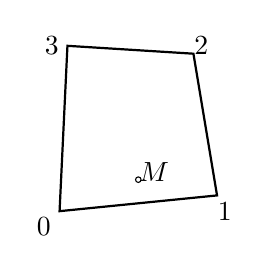
\begin{tikzpicture}
%\draw[step=0.5cm,gray,very thin] (0,0) grid (4,4); %background grid
\draw[thick] (1,1) -- (3,1.2) -- (2.7,3) -- (1.1,3.1) -- cycle;  
\node[] at (0.8,0.8) {0};
\node[] at (3.1,1) {1};
\node[] at (2.8,3.1) {2};
\node[] at (0.9,3.1) {3};
\node[] at (2.2,1.5) {$M$};
\draw (2.,1.4) circle (1pt);
\end{tikzpicture}\\
\end{center}

Several rather simple options exist:
\begin{itemize}
\item we could subdivide the quadrilateral into two triangles and check whether point $M$ is inside any of them (as it turns out, 
this problem is rather straightforward for triangles. Simply google it.)
\item We could check that point $M$ is always on the left side of segments $0\rightarrow 1$, $1\rightarrow 2$, $2\rightarrow 3$, $3\rightarrow 0$.
\item ...  
\end{itemize}

Any of these approaches will work although some might be faster than others. In three-dimensions all will however become 
cumbersome to implement and might not even work at all. Fortunately, there is an elegant way to answer the question, as 
detailed in the following subsection.

%-------------------------------------------
\subsubsection{Three-dimensional space}

If point $M$ is inside the quadrilateral, there exist a set of reduced coordinates $r,s,t\in[-1:1]^3$ such that 

\[
\sum_{i=1}^4 N_i(r_M,s,t) x_i = x_M
\quad\quad\quad
\sum_{i=1}^4 N_i(r_M,s,t) y_i = y_M
\quad\quad\quad
\sum_{i=1}^4 N_i(r_M,s,t) z_i = z_M
\]
This can be cast as a system of three equations and three unknowns. Unfortunately, each shape function $N_i$ 
contains a term $rst$ (as well as $rs$, $rt$, and $st$) so that it is not a linear system and standard techniques
are not applicable. 
We must then use an iterative technique: the algorithm starts with a guess for values $r,s,t$ and 
improves on their value iteration after iteration. 

The classical way of solving nonlinear systems of equations is Newton's method. 
\index{general}{Newton's method}
We can rewrite the equations above as ${\bm F}(r,s,t)=0$:
\begin{eqnarray}
\sum_{i=1}^8 N_i(r,s,t) x_i - x_M&=&0 \nonumber\\
\sum_{i=1}^8 N_i(r,s,t) y_i - y_M&=&0 \nonumber\\
\sum_{i=1}^8 N_i(r,s,t) z_i - z_M&=&0
\end{eqnarray}
or,
\begin{eqnarray}
F_r(r,s,t)&=&0 \nonumber\\
F_s(r,s,t)&=&0 \nonumber\\
F_t(r,s,t)&=&0 \nonumber
\end{eqnarray}

so that we now have to find the zeroes of continuously differentiable functions ${\bm F}:\mathbb{R} \rightarrow \mathbb{R}$.
The recursion is simply:
\[
\left(
\begin{array}{c}
r_{k+1} \\s_{k+1} \\ t_{k+1}
\end{array}
\right)
=
\left(
\begin{array}{c}
r_{k} \\s_{k} \\ t_{k}
\end{array}
\right)
- J_F(r_k,s_k,t_k) ^{-1} 
\left(
\begin{array}{c}
F_r(r_k,s_k,t_k) \\
F_s(r_k,s_k,t_k)\\
F_t(r_k,s_k,t_k)
\end{array}
\right)
\]
where $J$ the Jacobian matrix:
\begin{eqnarray}
J_F(r_k,s_k,t_k)
&=&
\left(
\begin{array}{ccc}
\frac{\partial F_r}{\partial r}(r_k,s_k,t_k) & \frac{\partial F_r}{\partial s}(r_k,s_k,t_k) & \frac{\partial F_r}{\partial t}(r_k,s_k,t_k) \\\\
\frac{\partial F_s}{\partial r}(r_k,s_k,t_k) & \frac{\partial F_s}{\partial s}(r_k,s_k,t_k) & \frac{\partial F_s}{\partial t}(r_k,s_k,t_k) \\\\
\frac{\partial F_t}{\partial r}(r_k,s_k,t_k) & \frac{\partial F_t}{\partial s}(r_k,s_k,t_k) & \frac{\partial F_t}{\partial t}(r_k,s_k,t_k) 
\end{array}
\right) \nonumber\\
&=&
\left(
\begin{array}{ccc}
\sum\limits_{i=1}^8 \frac{\partial N_i}{\partial r}(r_k,s_k,t_k) x_i &
\sum\limits_{i=1}^8 \frac{\partial N_i}{\partial s}(r_k,s_k,t_k) x_i &
\sum\limits_{i=1}^8 \frac{\partial N_i}{\partial t}(r_k,s_k,t_k) x_i \\
\sum\limits_{i=1}^8 \frac{\partial N_i}{\partial r}(r_k,s_k,t_k) y_i &
\sum\limits_{i=1}^8 \frac{\partial N_i}{\partial s}(r_k,s_k,t_k) y_i &
\sum\limits_{i=1}^8 \frac{\partial N_i}{\partial t}(r_k,s_k,t_k) y_i \\
\sum\limits_{i=1}^8 \frac{\partial N_i}{\partial r}(r_k,s_k,t_k) z_i &
\sum\limits_{i=1}^8 \frac{\partial N_i}{\partial s}(r_k,s_k,t_k) z_i &
\sum\limits_{i=1}^8 \frac{\partial N_i}{\partial t}(r_k,s_k,t_k) z_i 
\end{array}
\right) \nonumber 
\end{eqnarray}
In practice, we solve the following system:
\[
J_F(r_k,s_k,t_k) 
\left[  
\left(
\begin{array}{c}
r_{k+1} \\s_{k+1} \\ t_{k+1}
\end{array}
\right)
-
\left(
\begin{array}{c}
r_{k} \\s_{k} \\ t_{k}
\end{array}
\right)
\right]=-
\left(
\begin{array}{c}
F_r(r_k,s_k,t_k) \\
F_s(r_k,s_k,t_k)\\
F_t(r_k,s_k,t_k)
\end{array}
\right)
\]
Finally, the algorithm goes as follows:
\begin{itemize}
\item set guess values for $r,s,t$ (typically 0)
\item loop over k=0,...
\item Compute rhs= $-{\bm F}(r_k,s_k,t_k)$ 
\item Compute matrix $J_F(r_k,s_k,t_k)$
\item solve system for $(dr_k,ds_k,dt_k)$
\item update $r_{k+1}=r_k+dr_k$, $s_{k+1}=s_k+ds_k$, $t_{k+1}=t_k+dt_k$ 
\item stop iterations when $(dr_k,ds_k,dt_k)$ is small
\item if $r_k,s_k,t_k\in[-1,1]^3$ then $M$ is inside.
\end{itemize}
This method converges quickly but involves iterations, and multiple solves of $3\times 3$ systems which, 
when carried out for each marker and at each time step can prove to be expensive. 
A simple modification can be added to the above algorithm: iterations should be carried out {\it only}
when the point $M$ is inside of a cuboid of size $[\min\limits_i{x_i}:\max\limits_i{x_i}]\times[\min\limits_i{y_i}:\max\limits_i{y_i} ]
\times[\min\limits_i{z_i}:\max\limits_i{z_i}]$ where the sums run over the vertices of the element. 
In 2D this translates as follows: only carry out Newton iterations when $M$ is inside the red rectangle!
\begin{center}
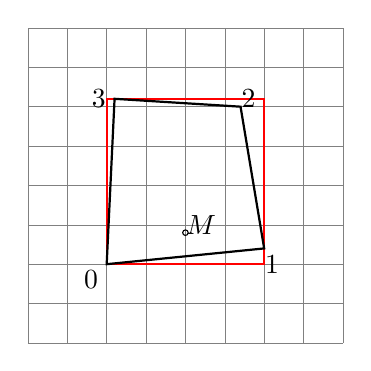
\begin{tikzpicture}
\draw[step=0.5cm,gray,very thin] (0,0) grid (4,4); %background grid
\draw[thick,red] (1,1) -- (3,1) -- (3,3.1) -- (1,3.1) -- cycle;  
\draw[thick] (1,1) -- (3,1.2) -- (2.7,3) -- (1.1,3.1) -- cycle;  
\node[] at (0.8,0.8) {0};
\node[] at (3.1,1) {1};
\node[] at (2.8,3.1) {2};
\node[] at (0.9,3.1) {3};
\node[] at (2.2,1.5) {$M$};
\draw (2.,1.4) circle (1pt);
\end{tikzpicture}\\
\end{center}

Note that the algorithm above extends to high degree elements such as $Q_2$ and higher, even with curved sides.


\todo[inline]{write about case when element is rectangle/cuboid}


 %---------
\newpage %-----------------------------------------------------------------------------------------
\subsection{Error measurements and convergence rates} \index{$L_1$ norm}
\index{$L_2$ norm}
\index{$H^1$ norm}

What follows is written in the case of a two-dimensional model. Generalisation to
3D is trivial. What follows is mostly borrowed from \cite{thmk14}.

When measuring the order of accuracy of the primitive variables $\vec{v}$ and $p$,
it is standard to report errors in both the $L_1$ and the $L_2$ norm.
For a scalar quantity $\Psi$, the $L_1$ and $L_2$ norms are computed as
\[
\norm{\Psi}_1 = \int_V |\Psi| dV
\quad\quad
\quad\quad
\norm{\Psi}_2 = \sqrt{ \int_V \Psi^2 dV }
\]
For a vector quantity $\vec{k}=(k_x,k_y)$ in a two-dimensional space,
the $L_1$ and $L_2$ norms are defined as:
\[
\norm{\vec{k}}_1 = \int_V (|k_x|+|k_y|) dV
\quad\quad
\quad\quad
\norm{\vec{k}}_2 = \sqrt{ \int_V (k_x^2+k_y^2) dV }
\]
To compute the respective norms
the integrals in the above norms can be approximated by splitting them
into their element-wise contributions. The element volume integral can then
be easily computed by numerical integration using Gauss-Legendre quadrature.

The respective $L_1$ and $L_2$ norms for the pressure error can be evaluated via
\[
e_p^h|_1 = \sum_{i=1}^{n_e} \sum_{q=1}^{n_q} |e_p^h(\vec{r}_q)| w_q |J_q|
\quad\quad
\quad\quad
e_p^h|_2=\sqrt{ \sum_{i=1}^{n_e} \sum_{q=1}^{n_q} |e_p^h(\vec{r}_q)|^2 w_q |J_q| }
\]
where $e_p^h(\vec{r}_q)=p^h(\vec{r}_q) - p(\vec{r}_q)$ 
is the pressure error evaluated at the $q$-th quadrature associated with
the $i$th element. $n_e$ and $n_q$ refer to the number of elements and
the number of quadrature points per element.
$w_q$ and $J_q$ are the quadrature weight of the Jacobian associated with
point $q$.

The velocity error $e_{\vec v}^h$ is evaluated using the following two norms
\[
e_{\vec{v}}^h|_1 = \sum_{i=1}^{n_e} \sum_{q=1}^{n_q} [ |e_u^h(\vec{r}_q)| + |e_v^h(\vec{r}_q)| ]    w_q |J_q|
\quad\quad
\quad\quad
e_{\vec v}^h|_2=\sqrt{ \sum_{i=1}^{n_e} \sum_{q=1}^{n_q} \left[ |e_u^h({\bm r}_q)|^2 +  e_v^h({\bm r}_q)|^2 \right] w_q |J_q| }
\]
where $e_u^h(\vec{r}_q)=u^h(\vec{r}_q) - u(\vec{r}_q)$ and $e_v^h(\vec{r}_q)=v^h(\vec{r}_q)-v(\vec{r}_q)$.




\index{$H^1(\Omega)$ space} \index{$H^1$ norm} \index{$H^1$ semi-norm}
Another norm is very varely used in the geodynamics literature but is preferred in the 
Finite Element literature: the so-called $H^1$ norm. The mathematical basis for this
norm and the nature of the $H^1(\Omega)$ Hilbert space is to be found in many FE books \cite{dohu03,john16,hugh}.
This norm is expression is expressed as follows for a function $f$ such that $f,|\nabla f|\in L^2(\Omega)$
\footnote{\url{https://en.wikipedia.org/wiki/Sobolev_space}}
\[
\norm{f}_{H^1} = \left( \int_\Omega ( |f|^2 + |\nabla f|^2  ) d\Omega   \right)^{1/2}
\]
We then have 
\[
e_{\vec v}^h|_{H^1} = \norm{\vec{v}^h-\vec{v}}_{H^1} = \sqrt{
\sum\limits_{i=1}^d 
\int_\Omega  
\left[
({v}_i^h-{v}_i)^2
+
\vec\nabla(v_i^h-v_i)\cdot\vec\nabla(v_i^h-v_i) 
\right] d\Omega   
}
\]
where $d$ is the number of dimensions.
Note that sometimes the following semi-norm is used \cite{dobo04,bodg06}:
\[
e_{\vec v}^h|_{H^1} = \norm{\vec{v}^h-\vec{v}}_{H^1} = \sqrt{
\sum\limits_{i=1}^d 
\int_\Omega  
\left[
\vec\nabla(v_i^h-v_i)\cdot\vec\nabla(v_i^h-v_i) 
\right] d\Omega   
}
\]
 

When computing the different error norms for $e_p$ and $e_{\vec v}$ for a set of numerical experiments with
varying resolution $h$ we expect the error norms to follow the following relationships:
\[
e_{\vec v}^h|_1 = C h^{rvL_1} 
\quad\quad\quad\quad
e_{\vec v}^h|_2 = C h^{rvL_2} 
\quad\quad\quad\quad 
e_{\vec v}^h|_{H^1} = C h^{rvH^1}
\]
\[
e_p^h|_1 = C h^{rpL_1} 
\quad\quad\quad 
e_p^h|_2 = C h^{rpL_2}
\]
where $C$ is a resolution-independent constant
and $rpXX$ and $rvXX$ are the convergence rates for
pressure and velocity in various norms, respectively. 
Using linear regression on the logarithm of the respective error norm and the resolution $h$,
one can compute the convergence rates of the numerical solutions.

As mentioned in \cite{dobo04}, when finite element solutions converge at
the same rates as the interpolants we say that the method is optimal, i.e.:
\index{optimal rate}

\[
e_{\vec v}^h|_{L_2} = {\cal O}(h^3)
\quad\quad\quad\quad
e_{\vec v}^h|_{H^1} = {\cal O}(h^2)
\quad\quad\quad\quad
e_{p}^h|_{L_2} = {\cal O}(h^2)
\]

%\begin{itemize}
%\item For $Q_1P_0$, the theoretical lower bound for $r_v'$ is 2 and for $r_p'$ it is 1
%\item For $Q_2P_{-1}$, the theoretical lower bound for $r_v'$ is 3 and for $r_p'$ it is 2
%\end{itemize}
We note that when using discontinuous pressure space
(e.g., $P_0$, $P_{-1}$), these bounds remain valid even
when the viscosity is discontinuous provided that the element boundaries conform to the discontinuity.

 
\subsubsection{About extrapolation}
\index{Extrapolation}

{\it Section contributed by W. Bangerth and part of Thieulot \& Bangerth [in prep.]}

In a number of numerical benchmarks we
want to estimate the error $X_h-X^\ast$ between a quantity $X_h$ computed
from the numerical solution $\vec{u}_h,p_h$ and the corresponding value
$X$ computed from the exact solution $\vec{u},p$. Examples of such quantities
$X$ are the root mean square velocity $v_{rms}$, but it could also be a mass flux
across a boundary, an average horizontal velocity at the top boundary, or
any other scalar quantity.

If the exact solution is known, then one can of course compute $X$ from it.
On the other hand, we would of course like to assess convergence also in
cases where the exact solution is not known. In that case, one can compute
an \textit{estimate} $X^\ast$ for $X$ by way of \textit{extrapolation}.
To this end, we make the assumption that asymptotically, $X_h$ converges to
$X$ at a fixed (but unknown) rate $r$, so that
\begin{equation}
  \label{eq:extrapolation-1}
  e_h=|X_h-X| \approx C h^r.
\end{equation}
Here, $X$, $C$ and $r$ are all unknown constants to be determined, although
we are not really interested in $C$.
We can evaluate $X_h$ from the numerical solution
on successively refined meshes with mesh sizes $h$, $h/2$, and $h/4$. Then,
in addition to \eqref{eq:extrapolation-1} we also have
\begin{eqnarray}
  \label{eq:extrapolation-2}
  e_{h/2}=|X_{h/2}-X| \approx C \left(\frac h2\right)^r,
  \\
  \label{eq:extrapolation-3}
  e_{h/4} =|X_{h/4}-X| \approx C \left(\frac h4\right)^r.
\end{eqnarray}
Taking ratios of equations \eqref{eq:extrapolation-1}--\eqref{eq:extrapolation-3},
and replacing the unknown $X$ by an \textit{estimate} $X^\ast$, we then
arrive at the following equation:
\begin{equation*}
\frac{|X_h-X^\star|}{|X_{h/2}-X^\star|}
=
\frac{|X_{h/2}-X^\star|}{|X_{h/4}-X^\star|}=2^r.
\end{equation*}
If one assumes that $X_h$ converges to $X$ uniformly either from above or
below (rather than oscillate around $X$), then this equation allows us
to solve for $X^\ast$ and $r$:
\begin{equation*}
X^\star = \frac{X_h X_{h/2}-X_{h/2}^2}{X_h - 2 X_{h/2} + X_{h/4}}, \qquad\qquad
r = \log_2 \frac{X_{h/2}-X^\star}{X_{h/4}-X^\star}.
\end{equation*}
In the determination of $r$, we could also have used $X_h$ and $X_{h/2}$,
but using $X_{h/2}$ and $X_{h/4}$ is generally more reliable because
the higher order terms we have omitted in \eqref{eq:extrapolation-1} are less
visible on finer meshes.

 %-----------------------------
\newpage %-----------------------------------------------------------------------------------------
\subsection{The initial temperature field} \subsubsection{Single layer with imposed temperature b.c.}

Let us take a single layer of material characterised by
a heat capacity $c_p$, a heat conductivity $k$
and a heat production term $H$.

\begin{center}
\includegraphics[width=5cm]{images/initial_temperature/tempcond.png}
\end{center}

The Heat transport equation writes
\[
\rho c_p ( \frac{\partial T}{\partial t} + {\vec v} \cdot {\vec \nabla} { T}) = 
{\vec \nabla} \cdot (k {\vec \nabla} T) + \rho H
\]
At steady state and in the absence of a velocity field, and assuming
that the material properties to be independent of time and space, and that
there is no heat production ($H=0$), this equation
simplifies to
\[
\Delta T =0 
\]
Assuming the layer to be parallel to the $x$-axis, this yields to write
\[
T(x,y)=T(y)=\alpha T+ \beta
\]
In order to specify the constants $\alpha$ and $\beta$, we need two constraints.

At the bottom of the layer $y=y_b$ a temperature $T_b$ is prescribed while a temperature
$T_t$ is prescribed at the top with $y=y_t$. This ultimately yields a temperature field in
the layer given by
\[
\boxed{
T(y) = \frac{T_t-T_b}{y_t-y_b}(y-y_b) + T_b
}
\]

If now the heat production coefficient is not zero, the differential equation
reads
\[
 k \Delta T + H = 0 
\]
The temperature field is then expected to be of the form
\[
T(y)= - \frac{H}{2k} y^2 + \alpha y + \beta 
\]
Supplied again with the same boundary conditions, this leads to
\[
\beta=T_b + \frac{H}{2k} y_b^2 - \alpha y_b
\]
ie,
\[
T(y) = -\frac{H}{2k} (y^2-y_b^2) + \alpha (y-y_b) + T_b
\]
and finally
\[
\alpha =  \frac{T_t-T_b}{y_t-y_b}  + \frac{H}{2k}(y_b+y_t)
\]
or,
\[
T(y) = -\frac{H}{2k} (y^2-y_b^2) + \left( \frac{T_t-T_b}{y_t-y_b}  + \frac{H}{2k}(y_b+y_t)   \right) (y-y_b) + T_b
\]

Taking $H=0$ in this equation obviously yields the temperature field obtained previously.
Taking $k=2.25$, $T_t=0C$, $T_b=550C$, $y_t=660km$, $y_b=630km$ yields the following
temperature profiles and heat fluxes when the heat production $H$ varies:
\begin{center}
\includegraphics[width=5cm]{images/initial_temperature/temperature1.pdf}
\includegraphics[width=5cm]{images/initial_temperature/heatflux1.pdf}
\end{center}
Looking at the values at the top, which are somewhat estimated to be
about $55-65mW/m^2$ \cite[table 8.6]{jama}, one sees that value $H=0.8e-6$ yields a very acceptable
heat flux.
Looking at the bottom, the heat flux is then about $0.03W/m^2$
which is somewhat problematic since the heat flux at the Moho
is reported to be somewhere between 10 and 20 $mW/m^2$ in \cite[table 7.1]{jama}.


%-----------------------------------------------------
\subsection{Single layer with imposed heat flux b.c.}

Let us now assume that heat fluxes are imposed at the top and bottom of the layer:
\begin{center} 
\includegraphics[width=5cm]{images/initial_temperature/tempcond2.png}
\end{center}

We start again from the ODE
\[
k \Delta T + H = 0 
\]
but only integrate it once:
\[
k \frac{dT}{dy}  + H y + \alpha  = 0 
\]
At the bottom $q=k(dT/dy)|_{y=y_b} = q_b$ and at the top
$q=k(dT/dy)|_{y=y_t} = q_t$ so that 

\todo[inline]{to finish}


 
%-----------------------------------------------------
\subsection{Single layer with imposed heat flux and temperature b.c. }

\begin{center}
\includegraphics[width=5cm]{images/initial_temperature/tempcond3.png}
\end{center}

\todo[inline]{to finish}


%---------------------------------------------------------------
\subsubsection{Half cooling space}

%---------------------------------------------------------------
\subsubsection{Plate model}

%---------------------------------------------------------------
\subsubsection{McKenzie slab}










 %---------------------------
\newpage %-----------------------------------------------------------------------------------------
\subsection{Kinematic boundary conditions}\label{kin_bc} \index{general}{Essential Boundary Conditions}
\index{general}{Natural Boundary Conditions}

Boundary conditions come in two basic flavors: essential and natural.
\begin{itemize}
\item Essential bcs directly affect DOFs, and are imposed on the FEM matrix. 
\item Natural bcs do not directly affect DOFs and are imposed on the right-hand side vector.
\end{itemize}

\subsubsection{In-out flux boundary conditions for lithospheric models}

\begin{center}
\includegraphics[width=8cm]{images/boundary_conditions/bc1}\\
\includegraphics[width=8cm]{images/boundary_conditions/drawing.png}
\end{center}

The velocity on the side is given by
\begin{eqnarray}
u(y) &=& v_{ext} \quad\quad y<L_1 \nn\\
u(y) &=& \frac{v_{in}-v_{ext}}{y_2-y_1}(y-y_1) + v_{ext} \quad\quad y_1<y<y_2 \nn\\
u(y) &=& v_{in} \quad\quad y>y_2 \nn
\end{eqnarray}
The requirement for volume conservation is:
\[
\Phi=\int_{0}^{L_y} u(y) dy = 0
\]
Having chosen $v_{in}$ (the velocity of the plate), one can then compute $v_{ext}$
as a function of $y_1$ and $y_2$.

\begin{eqnarray}
\Phi
&=&\int_{0}^{y_1} u(y) dy  +\int_{y_1}^{y_2} u(y) dy +\int_{y_2}^{L_y} u(y) dy \nn\\
&=& v_{ext} y_1  + \frac{1}{2}(v_{in}+v_{ext})(y_2-y_1) + (L_y-y_2) v_{in} \nn\\
&=& v_{ext} [y_1 + \frac{1}{2}(y_2-y_1) ] + v_{in} [ \frac{1}{2}(y_2-y_1)  + (L_y-y_2) ] \nn\\
&=& v_{ext}\frac{1}{2} (y_1 + y_2 ) + v_{in} [ L_y - \frac{1}{2}(y_1+y_1) ] \nn
\end{eqnarray}
and finally
\begin{mdframed}[backgroundcolor=blue!5]
\[
v_{ext} = -v_{in} \frac{ L_y - \frac{1}{2}(y_1+y_1)}{ \frac{1}{2} (y_1 + y_2 ) }
\]
\end{mdframed}

Note that in some cases applying free slip boundary conditions on a curved boundary with a triangular mesh 
can be problematic as explained in Dione \etal (2013) \cite{ditu13}.

\Literature \cite{ensg82}
 %--------------------
\newpage %-----------------------------------------------------------------------------------------
\subsection{Computing gradients - the recovery process} 
write about recovering accurate strain rate components and heat flux components on the nodes.

Let $\vec g(\vec r)$  be the desired nodal 
field which we want to be the continuous $Q_1$ representation of the field $\vec \nabla f^h$.
Since the derivative of the shape function does not exist on the nodes we need to design
an algorithm do do so. This problem is well known and has been 
investigated %\cite{XX.XXX}
\improvement{refs!}.
The main standard techniques are listed hereafter.


%..............................
\subsubsection{Global recovery}

The global recovery approach is rather simple: we wish to find $\vec g^h$
such that it satisfies
\[
\int_\Omega \phi \vec g^h \; d\Omega  = \int_\Omega \phi \vec\nabla f^h \; d\Omega 
\quad\quad \forall \phi
\] 
We will then successively replace $\phi$ by all the shape functions $N_i$ 
and since we have $g^h=\sum_j N_i g_i$ we then obtain
\[
\sum_j \int N_i N_j d\Omega g_i = \int N_i  \vec\nabla f^h \; d\Omega 
\]
or, 
\[
\mathbb{M} \cdot \vec{\cal G} = \vec f
\]



%..................................................
\subsubsection{Local recovery - centroid average over patch}





%..................................................
\subsubsection{Local recovery - nodal average over patch}

Let $j$ be the node at which we want to compute $\vec g$.
Then 
\[
\vec g_j = \vec g(\vec r_j) = 
\frac{\sum\limits_{ e \text{ adj. to }j} |\Omega_e| (\vec\nabla f)_e(\vec r_j) }{\sum |\Omega_e|}
\]
where $|\Omega_e|$ is the volume of the element and $(\vec\nabla f^h)_e(\vec r_j)$
is the gradient of $f$ as obtained with the shape functions inside element $e$ and 
computed at location $\vec r_j$.

%........................................................
\subsubsection{Local recovery - least squares over patch}



%........................................................
\subsubsection{Link to pressure smoothing}

When the penalty method is used to solve the Stokes equation, the pressure
is then given by $p=-\lambda \vec\nabla \cdot \vec v$. As explained in 
section \ref{sec_penalty}, the velocity is first obtained and the pressure 
is recovered by using this equation as a postprocessing step. Since the divergence 
cannot be computed easily at the nodes, the pressure is traditionally computed 
in the middle of the elements, yielding an elemental pressure field (remember, 
we are talking about $Q_1P_0$ elements here -- bi/tri-linear velocity, discontinuous
constant pressure)



\improvement{tie to fieldstone 12}

 %-------------------------
\newpage %-----------------------------------------------------------------------------------------
\subsection{Tracking materials and/or interfaces} \begin{flushright} {\tiny {\color{gray} tracking.tex}} \end{flushright}

Unless using a fully Lagrangian formulation, one needs an additional numerical method to represent/track
the various materials present in an undeformable (Eulerian) mesh.
The figure below (by B. Hillebrand) illustrates the three main methods used in geodynamics.

\begin{center}
\includegraphics[width=15cm]{images/tracking/tracking}
\end{center}

Note that what follows is applicable to FEM, FDM, etc ...


A typical test for advection algorithm is the Zalesak disk \cite{zale79}. It is a two dimensional test 
problem of solid body rotation with a constant angular velocity $\omega$ (in rad/sec):

\begin{center}
\includegraphics[width=6cm]{images/tracking/zale79a}
\includegraphics[width=6cm]{images/tracking/zale79b}\\
{\tiny Taken from \cite{zale79}. Left: Schematic representation of two dimensional 
solid body rotation problem. The field inside the cut out has value 3 and it is 1
outside. The rotational speed is such that one full revolution is effected in 
628 cycles. The width of the gap separating the two halves of the cylinder,
as well as the maximum extent of the "bridge" connecting the two halves, is 5 cells.
Right: Perspective view of initial conditions for the two dimensional! solid body rotation
problem. Note that only a $50\times50$ portion of the mesh centered on the cylinder is displayed.}
\end{center}

This benchmark is widely used in the literature \cite{stco91,supu00,vasv05,dilp06,basd08,zhbl14}.
Note that the Zalesak disc is often supplemented with a cone and a Gaussian features:

\begin{center}
\includegraphics[width=6cm]{images/tracking/leve96}\\
{\tiny Taken from \cite{leve96}. Initial data for solid rotation tests}
\end{center}

%..............................................
\subsubsection{The Particle-in-cell technique}\label{ss:pic}
\index{general}{Particle-in-Cell}  
\index{general}{Marker-and-Cell} 
\index{general}{PIC} 
\index{general}{MAC}

\begin{remark}
The terms 'particle' and 'marker' are commonly (and unfortunately) interchangeably used in the literature 
in the context of the particle-in-cell technique. However, one should be aware that the marker-and-cell (MAC) 
technique is something different: it was invented in the early 60's at the Los Alamos Laboratories by 
Harlow and Welch (1965) \cite{hawe65}. For more information on MAC see the review paper 
by McKee \etal (2008) \cite{mctf08}. 
Also, Tackley and King (2003) \cite{taki03} talk about the tracer-ratio method in the context of PIC... 
\end{remark}

The Particle-in-cell method is by far the most widely used in computational geodynamics. 
In its most basic form it is a rather simple method to implement and this probably owes to its success
and early adoption \cite{popo92}  in non-parallel codes such as \sopale \cite{full95}, 
I2VIS \cite{geyu03} or \citcoms \cite{mczh04} (Appendix~\ref{app:codes}).
It has been implemented in \aspect{} \cite{galh18} and the inherent load balancing issues arising from the 
parallel implementation as well as from the use of Adaptive Mesh Refinement are discussed. 
It has also been implemented in the MILAMIN code \cite{daks08} to study LLSVPs \cite{musd15}.

\begin{center}
\includegraphics[width=8cm]{images/tracking/crsg12}\\
{\captionfont One of the main problems of the PIC method is the fact that the interface 
between the fluid is not tracked explicitely, and if one uses a random distribution of 
particles the black dotted line reprensents the 'real' interface between the fluids 
while the red line is liekly to be the interface one would obtain based on the 
distribution of particles. Taken from Crameri \etal (2012) \cite{crsg12}.}
\end{center}

Samuel (2018) \cite{samu18} does a great job at explaining 
the core problem with PIC: {\it the method requires the method requires particle-mesh 
and mesh-particle mappings to be specified. These critical operations constitute a
major source of inaccuracy in the PIC solution \cite{mona85,dumg11,thmk14}. 
Indeed, while the Lagrangian advection alone is not prone
to significant numerical diffusion, particle–mesh mappings can introduce 
important amounts of dissipation. This is particularly true
when the spatial distribution of particles is not homogeneous, leading 
to areas in the vicinity of gridpoints that are not sufficiently
well sampled by particles, and other regions where the domain is
oversampled by particles. This recurrent sampling problem develops 
in regions characterized by strong deformation, and concerns
both compressible and incompressible flow \cite{waav15,pukp16}. 
The non-homogeneous sampling has two main
origins. \\
- The first one corresponds to inaccuracies in advecting the
Lagrangian particles \cite{meje04}. This aspect has drawn
the attention of a few recent studies \cite{waav15,pukp16}, 
which have proposed the use of conservative schemes to
map velocity components from the Eulerian grid to the Lagrangian
particles during their advection. Such schemes have shown to significantly 
improve the accuracy of the interpolation, and result in
a considerably more homogeneous spatial sampling. \\
- The second origin, which has received less attention, is related to the deforming
nature of the flow \cite{modm03}, and is completely independent 
of the accuracy of the numerical methods for interpolating
the velocities at particles’ locations. In fact, for a given velocity
field, particles should travel along their characteristics, and even in
the case of incompressible flows, the distance between characteristics 
can vary in general, and can strongly diverge or converge in
regions characterized by strong deformation. This naturally leads to
the development of a non-homogeneous spatial distribution of the
Lagrangian particles, even if the particles locations are perfectly
known.}



The basic methodology goes as follows:
\begin{enumerate}
\item distribute particles in the domain
\item assign a material identity (and/or any other quantity) to each of them
\item project particle quantities of the Eulerian nodes of the mesh
\item solve the Stokes equations for a new velocity field
\item interpolate the velocity onto the particles
\item move the particles with their respective velocities 
\item go back to step 3
\end{enumerate}  

As it turns out each step above needs to be carefully executed and is more difficult than it 
first looks. 

\paragraph{Distributing particles in the domain}. Let us assume we wish to distribute $N_p$ particles
in the domain. How large must $N_p$ be? To simplify, one end member could be 'as many particles as possible that fit in memory' 
while the other end member could be 'one per element/cell on average'. While the former does not necessarily guarantee a 
desired accuracy while being CPU and memory intensive, the latter will certainly lead to zones in the domain void 
of particles which will be problematic since the projection onto the mesh might yield zero values or very inaccurate values.
How many particles (per element/cell) will be enough?
Also, should the particles be randomly distributed in the domain or on some kind of regular grid? 
See \stone 13.

Taken from Tackley and King (2003) \cite{taki03}: "Tracers are initialized on a regular grid 
with each tracer perturbed from its grid position by a random amount of up to
$\pm$ half a grid spacing, in order to eliminate artifacts due to tracer alignment."


\paragraph{Averaging and projection}. This is a very critical step. Unfortunately, there is no community-wide
agreed-upon method. The problem at hand boils down to: at a given location $(\vec r)$ in space I need a
the value of a field which is carried by the particles. 
The first step is to find the particle(s) close to this point. If done naively, this is a very costly affair, 
and begs the question what 'close' means. Finding all particles within a radius $R$ of point $\vec r$ can 
be done very efficiently (e.g. with linked lists, Verlet lists, ...) but the choice 
of $R$ proves to be critical:
if too small, there may not be any particle inside the circle, and if too large there may be many particles 
inside the circle and the averaging over so many particles in space will prove to be over diffusive. 
In practice, the FD or FE mesh is used to provide an indication of $R$. 
In FDM, the four cells (or quarter cells) around
a node represent the volume of space containing the particles whose properties are to be averaged \cite{dumg11} 
as illustrated in the following figure:

\begin{center}
\includegraphics[width=12cm]{images/dumg11}\\
{\captionfont Taken from \cite{dumg11}. The "4-cell" and "1-cell" schemes for projecting 
properties defined on the markers (denoted by stars) onto a node (denoted by the solid circle). 
(A) The 4-cell scheme. The support of the interpolating function $N_i$ associated
with node $i$ is indicated by the shaded region. Only markers within the support of node $i$ 
contribute to the projection operation used to define the nodal value at $i$. The shape of 
the bilinear interpolation function for node $i$ is indicated in the lower frame. 
(B) The 1-cell scheme. The thick lines in the lower frame indicate the grid used to discretize the
Stokes equations, while the thin lines indicate the grid onto which marker properties are projected. 
The 1-cell scheme utilizes a compact support of size $\Delta x \times  \Delta y$. The support 
for nodes $r$, $s$, $t$ are indicated by the shaded regions. Only markers within the nodal 
support contribute to the projection operation for that node.}
\end{center}

Given that the FEM requires to compute integrals over each element, one could assume that 
only the particles inside the element will contribute 
to the average values assigned to the quadrature points (which I coin 'elemental approach'). 

However, one could also decide to first average the properties onto the nodes
before using these nodal values to assign values to the quadrature points (which I coin 'nodal approach'). 
In this case the FDM approach seen above could apply. 

Finally, in both FDM and FEM bi/trilinear basis functions are used for the interpolation as 
they can be interpreted as weighing functions. Higher order basis functions could also be used 
but the standard $Q_2$ basis functions (Section~\ref{sec:shpfct2d})
are 2-nd order polynomials which can take negative values (as opposed to the $Q_1$ 
basis functions which are strictly positive)
and this can pose problems: in some cases, although all values to be averaged are positive, 
their weighed average can be negative.
See Section~\ref{ss:bern} for concrete examples.

\underline{nodal approach}

\underline{elemental approach (1) - piece-wise constant interpolation} 

What follows is written with simplicity in mind, although more mathematical formulations 
can be found in the literature \cite{galh18}.

Assuming that we have established a list of particles tracking a field $f(\vec r)$ inside the 
element 
%and that each particle has an 
%associated weight $w_i$ (function of the location where the average is to be computed or not), 
we must now compute their average value $<f>$. 
The simplest approach which comes to mind is the arithmetic mean ($am$):
\[
\langle f\rangle_{am} = \frac{\sum\limits_{i=1}^n f_i}{n}
\]  
where $n$ is the number of particles inside the element.
In the case where $f$ is the (mass) density $\rho$, it is indeed what should be used. 
However, turning now to viscosity $\eta$, we know that its value can vary by many orders of magnitude 
over very short distances.
It is then likely that the average runs over values spanning values between 
$10^{18}\text{Pa s}$ and $10^{25} \text{Pa s}$.
As explained in \cite{scbe08} the arithmetic averaging tends to 'favour' large values: 
if the sum runs over 
10 particles, 9 carrying the value $10^{25}$ and 1 carrying the value $10^{19}$, 
the average value is then
\[
\langle\eta\rangle = \frac{9\cdot 10^{25}+1\cdot 10^{19}}{10} \simeq 0.9\cdot 10^{25}
\]
which is much much closer to $10^{25}$ than to $10^{19}$.
Other averagings are then commonly used, namely the geometric mean ($gm$)  and the 
harmonic mean ($hm$), defined as follows:
\[
\langle f\rangle_{gm} = \left( \prod_i f_i \right)^{1/n} 
\qquad
\text{or, }
\qquad
\log_{10} \langle f \rangle_{gm} = \frac{\sum\limits_{i=1}^{n} \log_{10} f_i }{n}  
\]
and 
\[
\langle f\rangle_{hm} = \left( \frac{\sum\limits_{i=1}^n \frac{1}{f_i} }{n}  \right)^{-1}
\qquad
\text{or, }
\qquad
\frac{1}{\langle f\rangle_{hm} } = \frac{\sum\limits_{i=1}^n  \frac{1}{f_i} }{n}  
\]
The geometric mean can be seen as a form of arithmetic mean of $\log_{10}$ values, 
while the harmonic mean can be seen as 
a form of arithmetic mean of the inverse values.

Looking back at the above example, the geometric mean of the viscosities is given by 
\[
\log \langle \eta\rangle_{gm} = \frac{9\cdot 25+1\cdot 19}{10} = 24.4 
\qquad \text{or,} \qquad 
\langle \eta\rangle_{gm} \simeq 2.5 \cdot 10^{24}
\]
and the harmonic mean:
\[
\langle\eta\rangle_{hm} \simeq \left( \frac{1}{10 \cdot  10^{19}} \right)^{-1} = 10^{20}
\]
We see that the harmonic mean tends to favour the small values. Also we recover the known property:
\begin{equation}
\langle f \rangle_{am}\quad  \geq \quad
\langle f \rangle_{gm}\quad  \geq \quad
\langle f \rangle_{hm} 
\end{equation}

%When all $f_i$ are equal to $f_0$ their computed average should also be equal to $f_0$. As a consequence the 
%weights $N_i$ should fulfil the condition $\sum\limits_{i=1}^n N_i=1$.
%If all weights are equal, then $N_i=1/n$ and the averagings become:

%\begin{equation}
%\langle f\rangle_{am} = \frac{1}{n} \sum\limits_{i=1}^n f_i
%\qquad
%\langle f\rangle_{gm} = \prod_i f_i^{1/n} 
%\qquad
%\langle f\rangle_{hm} = \left( \frac{1}{n}\sum_i^n \frac{1}{\phi_i} \right)^{-1}
%\end{equation}

Once a single average value has been computed for the whole element, then 
all quadrature points are assigned this value. 


\underline{elemental approach (2) - Least Squares Interpolation } 
One can revisit this topic on the grounds that 
with high(er) order elements optimal convergence is unlikely to be reached 
if viscosity (and density) are assumed to be constant inside each element (see  
\cite{galb19}). One could therefore use the least-square method to arrive at 
a functional representation of the field inside the element which is as 
close as possible (in the least-squares sense, then) to the particle-based field. 

Thielmann \etal (2014) \cite{thmk14} use the $Q_2P_{-1}$ element and introduce an element-wise interpolation
scheme based on a least squares fitting of the particle properties and choose the functional to 
be a linear function to match the pressure space. 
They define the error $\epsilon$ such that 
\[
\epsilon^2 = \sum_{i=1}^n ( \tilde{f}(x_i,y_i)-f_i)^2
\]
with $\tilde{f}(x,y)=a+bx+cy$. 
We then look for the minimum of $\epsilon^2$, i.e. $\vec\nabla(\epsilon^2)=0$ in the $\{a,b,c\}$ space.
So 
\begin{eqnarray}
0=\frac{\partial \epsilon^2}{\partial a} 
&=& 2\sum\limits_i ( \tilde{f}(x_i,y_i)-f_i) \nn\\
&=& 2\sum\limits_i ( a + bx_i +cy_i -f_i) \nn\\
&=& 2 \left[ a \sum\limits_i 1 + b \sum\limits_i x_i + c \sum y_i - \sum\limits_i f_i \right] \nn\\
0=\frac{\partial \epsilon^2}{\partial b} &=& 2\sum\limits_i ( \tilde{f}(x_i,y_i)-f_i) x_i \nn\\
&=& 2\sum\limits_i ( a + bx_i +cy_i -f_i) x_i \nn\\
&=& 2 \left[ a \sum\limits_i x_i  + b \sum\limits_i x_i^2 + c \sum x_i y_i - \sum\limits_i x_i f_i \right]\nn\\
0=\frac{\partial \epsilon^2}{\partial c} &=& 2\sum\limits_i ( \tilde{f}(x_i,y_i)-f_i) y_i \nn\\ 
&=& 2\sum\limits_i ( a + bx_i +cy_i -f_i) y_i \nn\\
&=& 2 \left[ a \sum\limits_i y_i + b \sum\limits_i x_i y_i + c \sum y_i^2 - \sum\limits_i y_if_i \right] \nn
\end{eqnarray}
so 
\[
\left( 
\begin{array}{ccc}
\sum\limits_i 1 & \sum\limits_i x_i & \sum\limits_i y_i \\
\sum\limits_i x_i & \sum\limits_i x_i^2 & \sum\limits_i x_iy_i \\
\sum\limits_i y_i & \sum\limits_i x_i y_i & \sum\limits_i y_i^2 
\end{array}
\right)
\cdot
\left(
\begin{array}{c}
a\\
b\\
c
\end{array}
\right)
=
\left(
\begin{array}{c}
\sum\limits_i f_i \\
\sum\limits_i x_i f_i \\
\sum\limits_i y_i f_i 
\end{array}
\right)
\]

We could also then decide to use a bi-linear function $\tilde{f}$, i.e.
\[
\tilde{f}(x,y)=a+bx+cy+dxy
\]
which lies in the $Q_1$ space of Taylor-Hood quadrilateral elements. In this case the error is 
\[
\epsilon^2 
= \sum_{i=1}^n ( \tilde{f}(x_i,y_i)-f_i)^2
= \sum_{i=1}^n (a+bx_i+cy_i + dx_iy_i -f_i)^2
\]
and one has to solve a $4\times 4$ system this time:
\[
\left( 
\begin{array}{cccc}
\sum\limits_i 1 & \sum\limits_i x_i & \sum\limits_i y_i & \sum\limits_i x_iy_i\\
\sum\limits_i x_i & \sum\limits_i x_i^2 & \sum\limits_i x_iy_i & \sum\limits_i x_i^2 y_i\\
\sum\limits_i y_i & \sum\limits_i x_i y_i & \sum\limits_i y_i^2 & \sum\limits_i x_iy_i^2\\ 
\sum\limits_i x_iy_i & \sum\limits_i x_i y_i & \sum\limits_i y_i^2 & \sum\limits_i x_i^2y_i^2  
\end{array}
\right)
\cdot
\left(
\begin{array}{c}
a\\
b\\
c\\
d
\end{array}
\right)
=
\left(
\begin{array}{c}
\sum\limits_i f_i \\
\sum\limits_i x_i f_i \\
\sum\limits_i y_i f_i \\
\sum\limits_i x_i y_i f_i 
\end{array}
\right)
\]


Once this linear system (or the previous one) has been solved we have obtained the coefficients $a,b,c(,d)$ 
which allow us to compute $\tilde{f}$ anywhere inside the element, and especially 
at the quadrature points. 

\begin{remark}
Using a different (bi)linear function $\tilde{f}$ for each element 
means that it is likely to be discontinuous 
from one element to another in regions of high gradients. 
\end{remark}

There is however one drawback with this approach (linear or bi-linear alike):
in the areas of steep gradients the computed coefficients can be such that 
the function $\tilde{f}$ evaluated on a quadrature point 
is negative  which 1) would be wrong but not numerically 
dramatic for density, 2) would be wrong and physically and numerically 
problematic for viscosity (a viscosity cannot be negative, and this would 
automatically destroy the SPD nature of the viscous block of the Stokes matrix).

This problem is discussed in Thielmann \etal (2014) in Section 3.2.1 and they 
call this "Over- and Under-shooting". A simple (iteratuve) 
fix is then designed which insures that the computed value is within user-defined 
acceptable bounds. This is also mentioned in \cite{galb19} but the authors 
explain that this problem was not encountered in the context of the publication.





\begin{remark}
Two variants of the PIC methods have been proposed: the Deformable PIC (DPIC) 
by Samuel (2018) \cite{samu18}, and the multiscale PIC in \cite{asmo12}.
\end{remark}

\begin{remark}
TO BE WRITTEN.
A word about the tracer ratio method. \cite{taki03}. 
Trim \etal (2020) show a modified method 
with a tracer repositioning algorithm designed to promote even tracer
coverage \cite{trlb20}. 
\end{remark}



See Stone~67 for a concrete example of Particle-In-Cell use and a detailed 
explanation of its implementation.



%.....................................................................
\paragraph{Interpolation of the velocity onto particles}.

Once the particle $i$ has been localised inside a given element (Section~\ref{sec:amiin}) 
and its reduced coordinates $(r,s,t)$ determined, the velocity at this location can 
be computed through the basis functions:
\[
\vec\upnu_i=\sum_{k=1}^m N_i(r,s,t) \vec\upnu_k
\]
This approach is not without problem: while the nodal velocities $\vec\upnu_k$ are such 
that\footnote{for incompressible flows, of course} 
$\vec\nabla\cdot\vec\upnu=0$ (in the weak sense), the computed velocity $\vec\upnu_i$ 
is not necessarily divergence-free! In order to remedy this, a 
Conservative Velocity Interpolation (CVI) has been proposed in \cite{waav15}.
Because the complete derivations for the CVI algorithm is quite large I 
have decided to make a new section about it (Section~\ref{sec:cvi}) rather than include it 
here.

%.....................................................................
\paragraph{Moving the particles}

This is discussed in the context of the Runge-Kutta Methods, see Section~\ref{sec:rkparticles}.



%..............................................
\subsubsection{The level set function technique}
\index{general}{Level-set Method} 
\index{general}{Level-set Function} 
\index{general}{LSM} 
\index{general}{LSF} 
\index{general}{ENO}

This method was developed in the 80's by Stanley Osher and James Sethian \cite{lofo06}

The Level-set Method (LSM), as it is commonly used in Computational Fluid Dynamics -- and especially 
in Computational Geodynamics -- represents a close curve $\Gamma$ (say, in our case, the 
interface between two fluids or layers) by means of a function $\phi$ (called the level-set function, or LSF).
$\Gamma$ is then the zero level-set of $\phi$:
\begin{equation}
\Gamma = \left\{ (x,y) \; |\; \phi(x,y)=0 \right\}
\end{equation}
The convention is that $\phi>0$ inside the region delimited by $\Gamma$ and $\phi<0$ outside.
The function value indicates on which side of the
interface a point is located (negative or positive) and this is
used to identify materials. 

Furthermore, if the curve $\Gamma$ moves with a velocity $\vec \upnu$, 
then it satisfies the following equation:
\begin{equation}
\frac{\partial \phi}{\partial t} + \vec\upnu \cdot \vec\nabla \phi = 0 
\end{equation}

The level set function is generally chosen to
be a signed distance function, i.e. $|\vec\nabla \phi| = 1$ everywhere 
and its value is also the distance to the interface.

As explained in \cite{hitg14}, the level-set function $\phi$ is advected 
with the velocity $\vec\upnu$ which is obtained by solving the Stokes equations.
This velocity does not guarantee that after an advection step the signed 
distance quality of the LSF is preserved. 
The LSF then needs to be corrected, which is also called reinitialisation. 
Finally, solving the advection equation must be done in an accurate manner both in time and space,
so that so-called ENO (essentially non-oscillatory) schemes are often employed for the 
space derivative \cite{ossh91,saev10}.


The level set method has not often been used in the geodynamics 
community with some notable exceptions 
\cite{bomh06,bomh07,habm07,grbh07,zlfd08,hagr10,sunh10,suhe10,hitg14}
An overview of the method and applications can
be found in \cite{osfe01}.

Several improvements upon the original LSM have been proposed, 
such as for instance the conservative level set of \cite{zhbl14}.
The most notable difference between CLS method originally proposed by Olsson \etal \cite{olkr05,olkz07}
and standard LS method lies in the choice of LS function. Instead of the signed distance function, the
CLS methods employ the Heaviside function $H(\phi)$ 
\[
H(\phi)=
\left\{
\begin{array}{ll}
1 & \phi>0 \\
1/2 & \phi=0 \\
0 & \phi<0
\end{array}
\right.
\]
where $\phi$ is the signed distance function as in the LSM. 
In practice, a hyperbolic tangent function is used:
\[
H(\phi) = \frac{1}{2} (1+\tan (\phi/2\epsilon))
\]
where $\epsilon$ defines the spreading width of $H$. In the case where there are only 
two fluids (i.e. a single level set is sufficient), the material properties such as density and viscosity
are computed as follows:
\[
\rho=\rho_1+(\rho_2-\rho_1)H(\phi)
\]
\[
\eta=\eta_1+(\eta_2-\eta_1)H(\phi)
\]

\Literature: \cite{vasv05,vasv08,migi07,vasv05b}. 
\begin{itemize}
\item Review of level-set methods \cite{gifo18}
\item Interactive 3-D computation of fault surfaces using level sets \cite{kadt08}
\end{itemize}

%..............................................
\subsubsection{The field/composition technique \label{sec:compfield}}
\index{general}{Compositional Field}

This is the approach taken by the \aspect{} developers \cite{krhb12,hedg17}. 
Each material $i$ is represented by a compositional field $c_i$, 
which takes values between 0 and 1.
Each compositional field is then advected with the (prescribed or computed) Stokes velocity \cite{chri92}:
\begin{equation}
\frac{\partial c_i}{\partial t} + {\bm v}\cdot {\bm \nabla }c_i = 0
\end{equation}
The value at a point (Finite element node or quadrature point) is 1 if it is in the 
domain covered by the material $i$, and 0 otherwise.
In one dimension, each compositional field is a Heavyside function. 
This approach is somewhat similar to the LSM but the field is essentially 
discontinuous across the interface, which makes it very difficult to advect.  
On the plus side, compositional fields need not be reinitialised, as opposed to LSF's.

Accurate numerical advection is a notoriously difficult problem. Unless very specialised 
techniques are used it often yields undershoot ($c_i<0$) and overshoot ($c_i>0$), which 
ultimately yields mass conservation issues. Also, unless special care is taken, 
compositional fields tend to become more and more diffuse over time: the SUPG method (Section~\ref{sec:supg})
and the entropy viscosity method \cite{krhb12,ropu19} add small amounts of diffusion to dampen the under- and 
overshoots. This means that at a given point two or more compositions may have values, 
which require some form of averaging. If under- and overshoots are present, these averagings
can become very problematic and even yield meaningless quantities (e.g. negative viscosities).

One rather old and popular filtering approach is the so-called Lenardic and Kaula (1993) \cite{leka93}
filter:

\begin{center}
\includegraphics[width=6cm]{images/compositions/leka93_filter1}\\
\includegraphics[width=6cm]{images/compositions/leka93_filter2}\\
{\captionfont Taken from Lenardic and Kaula \cite{leka93}}
\end{center}

\begin{center}
\includegraphics[width=16cm]{images/compositions/leka93_filter3}\\
{\captionfont From FENICS book}
\end{center}


\begin{center}
\includegraphics[width=8cm]{images/compositions/plth13}\\
{\captionfont 
Filtering approach proposed by Lenardic and Kaula (1993). 
The composition field $C$ is assumed to vary between 0 and 1. Grid points with $C$-values 
lower than 0 and greater than 1 are set to 0 and 1, respectively (red). 
$C_{min}$ and $C_{max}$ are the minimum and maximum spurious values observed. 
Grid points whose $C$-value is lower than $|C_{min}|$ or greater than ($2-C_{max}$) 
are also set to 0 and 1, respectively (blue). 
The $C$-value of all grid points that do not exhibit spurious oscillations (green) is then corrected
according to the difference between the original average composition and that computed after the reset-
ting of the spurious values.
Taken from Plesa \etal (2013) \cite{plth13}.}
\end{center}











\Literature: \cite{vyrc13}

Entropy viscosity method \cite{gupa11}

\improvement[inline]{write about DG approach}






%..............................................
\subsubsection{The Volume-of-Fluid method} 
\index{general}{Volume-of-Fluid Method}
\index{general}{VOF}

%from Napoleon \etal
The Volume-Of-Fluid (VOF) method is a fixed-grid approach based on the one-fluid model and considers that the various immiscible fluids (or `phases') can be described as a single fluid whose local physical properties, namely density and viscosity, vary in space and time depending on the volume fraction $C_i$ of each phase $i$ 
\cite{hini81,youn82}. 

The volume fraction of each fluid intrinsically obeys $\sum \limits_{{i=1}}^n C_i = 1$ where $n$ is the number of phases. 
Typically, $C_i=1$ in grid cells filled only with fluid $i$, and $0<C_i<1$ in grid cells cross--cut by an interface. 
There are two main classes of VOF methods: methods that try to reconstruct exactly the interface between fluids (e.g. \cite{puth18}), which requires significant computational time, and methods that do not, such as in JADIM and OpenFOAM. 
With no interface reconstruction, the thickness of the interfacial region is defined by $0<C_i<1$, and typically occupies two to three grid cells. 

\cite{hini81}\cite{ropu19}

See review of the method in Robey's phd thesis \cite{robe19}.


%..............................................
\subsubsection{The method of characteristics}

\todo[inline]{ask Arie to write something}

\cite{devv00a}

%.............................................
\subsubsection{The Marker Chain method}
\index{general}{Marker Chain method} 

In two dimensions, the idea is quite simple: each interface is discretised by means of a number
of Lagrangian points (which may or may not vary in time). The points are numbered and 
connected (think of the connectivity array of a 1D FEM code). In the case of small deformations, 
and in the absence of in/out-flow boundaries, the method is reasonably trivial to implement, and 
each couple of point defines a segment (and therefore its normal vector too) which can then be used
to answer the question: "at this location, am I above or below this interface" or "am I this domain our
outside this domain" (in the case that the interface does not reach any of the boundaries).

This method becomes somewhat impractical when large deformation occurs or, for example, 
when a domain splits into two (e.g. slab break off). One interface must then become two, 
and it requires an algorithm capable of detecting the breakup of the surface and capable 
of rebuilding/patching the new ones so that they can still be used further. 
Note that in case of large deformation some markers may get further and further apart 
from each other which makes for a poor representation of the surface. New markers should then 
be added but the question of when and where must then be addressed.

Also, switching to three dimensions can prove to be very difficult or simply very 
costly: the generation of the inital marker position is trivial but their connectivity 
can be complicated to establish at startup: for instance, a Stokes sphere will require
a mesh made of triangles which maps exactly the surface of the sphere (see \cite{thie18,moma19} 
for methods on how to efficiently produce such meshes). In the case of more complex 3D geometries
this may prove nearly impossible to do. So will the problem of splitting a surface into two 
(or merging two domains). \todo{I still have pics from the old days using \douar- include} 

This method is usually coupled to Eulerian meshes (typically with FDM, but not only). 
It was used in \cite{woid78} in the context of salt domes analysis and later in \cite{chri82,chyu84}.
It is also used in \cite{vaks97} but little details are given about the algorithms used
to track and update the chain in the presence of such large deformation.
It is also used (athough coupled to level set functions) in the \douar code\cite{brtf08} 
(see Section~\ref{app:codes}). Having worked myself on this code and having had to produce 
complex initial triangulated surfaces for simulations (see for example \cite{lobh10}) it is 
easy to understand why later users of this code did implement the marker-in-cell technique.
More recently, it is used to track the free surface position in a FDM code \cite{dumy16,chmd19}.

Finally, Christensen \cite{chri92} makes the following interesting comment:  
"One might assume that different methods 
of representing the discontinuity, for example, by a tracer chain \cite{chyu84} or a cloud of 
tracers, would solve these problems. However, the difficulties 
arise not only from the way in which material boundaries are 
represented. Physically, the rate of shear strain parallel to a 
rheological boundary is discontinuous. Within the finite ele-
ment scheme such jump can only be realized at an element 
boundary. In an Eulerian scheme, where the discontinuity will 
crosscut the elements, the jump in strain rate must be approx- 
imated by a continuous variation, and effectively, the rheolog-
ical properties on both sides of the discontinuity will be 
averaged in some way within the element."

Literature: Lin \& van Keken (2006) \cite{liva05,liva06a,liva06b,kaus05,mulyukova}

%..............................................
\subsubsection{Hybrid methods}

In Braun \etal \cite{brtf08} a level set method is presented which is based on a 3-D set
of triangulated points, which makes it a hybrid between tracers and level set functions:
in the \douar code (Appendix~\ref{app:codes}) the interface is then explicitely tracked by means of the tracers while the LSF is computed 
on the FE nodes. Although very promising in theory, this method proved to be difficult to use in practice
since it requires a) a triangulation of the interfaces at $t=0$ which is not trivial if the geometries
are complex (think about a slab in 3D); b) the addition or removal of tracers because of the interface deformation
and the patching of the triangulation; c) the calculation of the distance to the interfaces for each 
FE node based on the triangle normal vectors. 
This probably explains why the Particle-In-Cell method was later implemented in this code (pers. comm.).
Note that another very similar approach is used in \cite{saev10}.



%..............................................
\subsubsection{Boundary fitted mesh}

This method is rather simple to implement and works well for small deformations. It is 
for instance used by Frehner \cite{freh14} (see online supplementary material) in which it is 
stated: "The numerical grid is set up in such a way that the interface
between different material phases (two layers in this case) coincides with element boundaries. Hence, each
element belongs to a unique material phase and no interpolation is necessary."
With such a method, each element is initally attributed a material phase/number and its material
properties do not change. 


\vspace{2cm} 

\Literature: three-dimensional front tracking method using a triangular mesh \cite{sclo03}.







 %-------------------------------
\newpage %-----------------------------------------------------------------------------------------
\subsection{Static condensation} \index{general}{Static Condensation}

The idea behind static condensation is quite simple: in some cases, there are dofs 
belonging to an element which only belong to that element. For instance, the so-called MINI 
element ($P_1^+ \times P_1$) showcases a bubble function in the middle (see section \ref{ss:pair}). 
In the following, $\vec{\cal V}^\star$ corresponds to the list of such dofs inside an element.
The discretised Stokes equations on any element looks like:

\begin{equation}
\left(
\begin{array}{ccc}
\K   & L & \G \\
L^T & \K^\star  & H \\
\G^T & H^T & 0
\end{array}
\right)_e
\left(
\begin{array}{c}
\vec{\cal V} \\ \vec{\cal V}^\star \\ \vec{\cal P}
\end{array}
\right)_e
=
\left(
\begin{array}{c}
\vec{f} \\ \vec{f}^\star \\ \vec{h}
\end{array}
\right)_e
\end{equation}
This is only a re-writing of the elemental Stokes matrix where the matrix $\K$ has been 
split in four parts.
Note that the matrix $\K^\star$ is diagonal.\todo{check}

This can also be re-written in non-matrix form:
\begin{eqnarray}
\K \cdot \vec{\cal V} + L \cdot \vec{\cal V}^\star + \G \cdot \vec{\cal P} &=& \vec{f} \\
L^T V + K^\star \cdot  \vec{\cal V}^\star + H \cdot \vec{\cal P} &=& \vec{f}^\star \\
\G^T \cdot \vec{\cal V} + H^T \vec{\cal V}^\star &=& \vec{h}
\end{eqnarray}
The $\vec{\cal V}^\star$ in the second equation can be isolated:
\[
\vec{\cal V}^\star = \K^{-\star} \cdot ( \vec{f}^\star - L^T \cdot \vec{\cal V} - H \cdot \vec{\cal P})
\]
and inserted in the first and third equations:
\begin{eqnarray}
\K \cdot \vec{\cal V} + L \left[ \K^{-\star} ( \vec{f}^\star - L^T \cdot \vec{\cal V} - H \cdot \vec{\cal P} )  \right] + \G \cdot \vec{\cal P} &=& \vec{f} \\
\G^T \cdot \vec{\cal V} + H^T \left[  \K^{-\star} ( \vec{f}^\star - L^T \cdot \vec{\cal V} - H \cdot \vec{\cal P}) \right]  &=& \vec{h}
\end{eqnarray}
or,
\begin{eqnarray}
(\K-L\cdot \K^{-\star} \cdot L^T)\cdot \vec{\cal V} + (G-L\cdot \K^{-\star} \cdot H) \cdot \vec{\cal P} &=& \vec{f}-L\cdot \K^{-\star} \cdot \vec{f}^\star \\
(G^T -H^T\cdot \K^{-\star}\cdot  L^T ) \cdot \vec{\cal V}  - 
(H^T \cdot \K^{-\star} \cdot H )\cdot \vec{\cal P}   &=& \vec{h} -H^T\cdot \K^{-\star}\cdot \vec{f}^\star
\end{eqnarray}
i.e.
\begin{eqnarray}
\underline{\K} \cdot \vec{\cal V} + \underline{\G}\cdot \vec{\cal P} &=& \underline{\vec{f}} \\
\underline{\G}^T \cdot \vec{\cal V} - \underline{\C} \cdot \vec{\cal P} &=& \underline{\vec{h}}
\end{eqnarray}
with
\begin{eqnarray}
\underline{\K}&=& K-L\cdot \K^{-\star} \cdot L^T \\
\underline{\G}&=& G-L\cdot \K^{-\star} \cdot H \\
\underline{\C}&=& H^T \cdot \K^{-\star} \cdot H \\
\underline{\vec{f}}&=& \vec{f}-L\cdot \K^{-\star} \cdot \vec{f}^\star \\
\underline{\vec{h}}&=& \vec{h} -H^T\cdot \K^{-\star}\cdot \vec{f}^\star
\end{eqnarray}
Note that $\underline{\K}$ is symmetric, and so is the Stokes matrix.


For instance, in the case of the MINI element, the dofs corresponding to the bubble 
could be eliminated at the elemental level, which would make the Stokes matrix smaller
(see book by Braess \cite{braess}). 
However, it is then important to note that static condensation introduces a 
pressure-pressure term which was not there in the original formulation.









 %-------------------------------------
\newpage %-----------------------------------------------------------------------------------------
\subsection{Measuring incompressibility \label{ss_incomp}} 
The velocity divergence error integrated over the whole element is given by
\begin{equation}
e_{div}= \int_\Omega (\vec\nabla\cdot \vec v^h - \underbrace{\vec\nabla\cdot \vec v}_{=0}  ) \; d\Omega
= \int_\Omega (\vec\nabla\cdot \vec v^h) \; d\Omega
\end{equation}
where $\Gamma_e$ is the boundary of element $e$ and $\vec{n}$ is the unit 
outward normal of $\Gamma_e$.

Furthermore we also have \cite{dobo04}:
\[
e_{div}
= \int_{\Gamma_e} \vec{v}^h\cdot\vec{n} \;  d\Gamma
\]
The reason is as follows and is called the divergence theorem:
suppose a volume $V$ subset of $\mathbb{R}^d$ which is compact
and has a piecewise smooth boundary $S$, and if $\vec F$ is
a continuously differentiable vector field then
\[
\int_V ( \vec\nabla\cdot\vec F)\; dV = \int_S (\vec F \cdot \vec n)\; dS
\]
The left side is a volume integral while the right side is a surface integral.
Note that sometimes the notation $d\vec S = \vec n \; dS $ is used so that 
$\vec F \cdot \vec n \; dS = \vec F \cdot d\vec S$.

The average velocity divergence over an element can be defined as 
\[
<\vec \nabla \cdot \vec v>_e 
= \frac{1}{V_e} \int_{\Omega_e}  (\vec\nabla\cdot\vec v) \; d\Omega
= \frac{1}{V_e} \int_{\Gamma_e} \vec{v}\cdot\vec{n} \; d\Gamma
\]
Note that for elements using discontinuous pressures we shall 
recover a zero divergence element per element (local mass conservation)
while for continuous pressure elements the mass conservation 
is guaranteed only globally (i.e. over the whole domain), see section 3.13.2 of \cite{grsa}.

Note that one could instead compute $<|\vec\nabla\cdot \vec v|>_e$. Either volume or 
surface integral can be computed by means of an appropriate Gauss-Legendre quadrature algorithm.

\improvement[inline]{implement and report}


 %------------------------
\newpage %-----------------------------------------------------------------------------------------
\subsection{Periodic boundary conditions\label{ss_periodic}}
This type of boundary conditions can be handy in some specific cases such 
as infinite domains. The idea is simple: when material leaves the domain 
through a boundary it comes back in through the opposite boundary (which 
of course presupposes a certain topology of the domain). 

For instance, if one wants to model a gas a the molecular level and wishes 
to avoid interactions of the molecules with the walls of the container, 
such boundary conditions can be used, mimicking an infinite domain in all 
directions. 

Let us consider the small mesh depicted hereunder:

We wish to implement horizontal boundary conditions so that 
\[
u_5=u_1
\quad\quad
u_{10}=u_6
\quad\quad
u_{15}=u_{11}
\quad\quad
u_{20}=u_{16}
\]
One could of course rewrite these conditions as constraints and extend the Stokes 
matrix but this approach turns out to be not practical at all. 

Instead, the method is rather simple: replace in the connectivity array the dofs on the right side
(nodes 5, 10, 15, 20) by the dofs on the left side. In essence, we wrap the system upon itself 
in the horizontal direction so that elements 4, 8 and 12 'see' and are 'made of' the nodes 1, 6, 11 and 16.
In fact, this is only necessary during the assembly. Everywhere in the loops nodes 5, 10, 15 and 20 appear 
one must replace them by their left pendants 1, 6, 11 and 16. This autmatically generates a matrix 
with lines and columns corresponding to the $u_5$, $u_{10}$, $u_{15}$ and $u_{20}$ being exactly zero. 
The Stokes matrix is the same size, the blocks are the same size and the symmetric character of the matrix 
is respected. However, there is a remaining problem. There are zeros on the diagonal 
of the above mentioned lines and columns. One must then place there 1 or a value more
appropriate.

Another way of seeing this is as follows: let us assume we have built and assembled
the Stokes matrix, and we want to impose periodic b.c. so that dof $j$ and $i$ are the same. 
The algorithm is composed of four steps:
\begin{enumerate} 
\item add col $j$ to col $i$
\item add row $j$ to row $i$ (including rhs)
\item zero out row $j$, col $j$
\item put average diagonal value on diagonal ($j,j$)
\end{enumerate} 

\begin{remark}
Unfortunately the non-zero pattern of the matrix with periodic b.c. is not the same 
as the matrix without periodic b.c.
\end{remark}


 %---------------------
\newpage %-----------------------------------------------------------------------------------------
\subsection{Removing rotational nullspace\label{ss_nullspace}} \index{general}{Angular Velocity} 
\index{general}{Angular Momentum} 
\index{general}{Moment of Inertia}

When free slip boundary conditions are prescribed in an annulus or
hollow sphere geometry there exists a rotational nullspace, or in other words there exists
a tangential velocity field ('pure rotation') which, 
if added or subtracted to the solution, genrates a solution which is still the solution of the PDEs. 

As in the pressure normalisation case (see section \ref{ss_pnorm}), the solution is simple:
\begin{enumerate}
\item fix the tangential velocity at {\it one} node on a boundary, and solve the sytem (the nullspace 
has been removed)\footnote{\url{https://scicomp.stackexchange.com/questions/3531/how-to-remove-rigid-body-motions-in-linear-elasticity}}
\item post-process the solution to have the velocity field fulfill the required conditions, i.e.
either a zero net angular momentum or a zero net angular velocity of the domain. 
\end{enumerate}

\begin{remark}
In \aspect{} this is available under the option 
"Remove nullspace = angular momentum" and "Remove nullspace = net rotation".
The "angular momentum" option removes a rotation such that the net angular momentum is zero.
The "net rotation" option removes the net rotation of the domain.
\end{remark}

%____________________________________
\paragraph{Angular momentum approach}

In order to remove the angular momentum, we search for a rotation
vector ${\vec \omega}$ such that
\begin{equation}
\int_\Omega \rho[{\vec r} \times ({\vec v}-{\vec \omega} \times {\vec r})] \; dV= \vec 0
\end{equation}

The angular momentum of a rigid body can be obtained from the sum 
of the angular momentums of the particles forming the 
body\footnote{\url{http://www.kwon3d.com/theory/moi/iten.html}}:
\begin{eqnarray}
\vec H 
&=& \sum_i \vec L_i\\
&=& \sum_i \vec r_i \times m_i \vec v_i\\
&=& \sum_i \vec r_i \times m_i (\vec \omega_i \times \vec r_i)\\
&=& \sum_i m_i 
\left(
\begin{array}{ccc}
\sum_i m_i(y_i^2+z_i^2) & -\sum_i m_i x_iy_i & -\sum_i m_i x_i z_i \\
-\sum_i m_i x_iy_i & \sum_i m_i(x_i^2+z_i^2) & -\sum_i m_i y_i z_i \\
-\sum_i m_i x_i z_i & -\sum_i m_i y_i z_i & \sum_i m_i(x_i^2+y_i^2)
\end{array}
\right)
\cdot
\left(
\begin{array}{c}
\omega_x \\ \omega_y \\ \omega_z
\end{array}
\right)
\end{eqnarray}
In the continuum limit, we have:
\begin{equation}
{\vec H} = \int_\Omega \rho(\vec r) \, {\vec r} \times {\vec v}\; dV
\end{equation}
and the $3\times3$ moment of inertia tensor $\bm I$
(also called inertia tensor) is given by\footnote{\url{https://en.wikipedia.org/wiki/Moment\_of\_inertia}}
\begin{equation}
{\bm I}= 
\int_\Omega \rho(\vec r) [\vec r\cdot\vec r \; \bm 1 - \vec r \times \vec r  ] dV
\end{equation}
so that the above equation writes:
$
{\vec H}={\bm I}\cdot {\vec \omega}
$
and then ${\vec \omega}={\bm I}^{-1} \cdot {\vec H}$.

Ultimately, at each velocity node a rotation about the rotation 
vector ${\vec \omega}$ is then subtracted from the velocity 
solution \cite[eq. 26]{zhmt08}:
\begin{equation}
\vec v_{new} = \vec v_{old} - \vec \omega \times \vec r 
\end{equation}


%____________________________________
%\paragraph{Angular velocity approach}

%The angular velocity\footnote{\url{https://en.wikipedia.org/wiki/Angular_velocity }}
% vector is given by $\vec\omega = \frac{\vec r\times \vec v}{r^2}$
%so that the volume-averaged angular velocity of the cylindrical shell is:
%\begin{equation}
%\vec {\omega} = \frac{1}{|\Omega|} \int_\Omega \frac{{\vec r}\times {\vec v}}{r^2} dV
%\end{equation}


%...............................
\subsubsection{Three dimensions}

The angular momentum vector is given by:
\begin{equation}
\vec H 
= \int_\Omega \rho(\vec r) \left( 
\begin{array}{c} 
yw-zv \\ zu-xw \\ xv-yu 
\end{array} \right) d\vec r
= 
\left(\begin{array}{c} 
\int_\Omega \rho(\vec r) (yw-zv) d\vec r\\
\int_\Omega \rho(\vec r) (zu-xw) d\vec r\\
\int_\Omega \rho(\vec r) (xv-yu) d\vec r
\end{array} \right)
= 
\left( 
\begin{array}{c} 
H_x \\ H_y \\ H_z
\end{array} \right)
\end{equation}
while the inertia tensor for a continuous body is given 
by
\begin{eqnarray}
\bm I
&=&\int_\Omega \rho(\vec r) [\vec r\cdot\vec r \; \bm 1 - \vec r \times \vec r  ] d\vec r \\
&=&\int_\Omega \rho(\vec r) 
\left[
\left(
\begin{array}{ccc}
x^2+y^2+z^2 & 0 & 0 \\
0 & x^2+y^2+z^2 & 0 \\
0 & 0 & x^2+y^2+z^2
\end{array}
\right)
- 
\left(
\begin{array}{ccc}
xx & xy & xz \\
yx & yy & yz \\
zx & zy & zz 
\end{array}
\right)
\right] 
d\vec r \\
&=&\int_\Omega \rho(\vec r) 
\left(
\begin{array}{ccc}
y^2+z^2 & -xy & -xz \\
-yx & x^2+z^2 & -yz \\
-zx & -zy & x^2+y^2 
\end{array}
\right)
d\vec r \\
&=&
\left(
\begin{array}{ccc}
\int_\Omega \rho(\vec r) (y^2+z^2) d\vec r & 
-\int_\Omega \rho(\vec r) xy d\vec r & 
-\int_\Omega \rho(\vec r) xz d\vec r \\\\
-\int_\Omega \rho(\vec r) yx d\vec r & 
\int_\Omega \rho(\vec r) (x^2+z^2) d\vec r & 
-\int_\Omega \rho(\vec r) yz d\vec r \\\\
-\int_\Omega \rho(\vec r) zx d\vec r & 
-\int_\Omega \rho(\vec r) zy d\vec r & 
\int_\Omega \rho(\vec r) (x^2+y^2) d\vec r 
\end{array}
\right)\\
&=&
\left(
\begin{array}{ccc}
I_{xx} & I_{xy} & I_{xz} \\
I_{yx} & I_{yy} & I_{yz} \\
I_{zx} & I_{zy} & I_{zz} 
\end{array}
\right)
\end{eqnarray}


%-----------------------------
\subsubsection{Two dimensions}

In two dimensions, flow is taking place in the $(x,y)$ plane. 
This means that $\vec r=(x,y,0)$ and $\vec v=(u,v,0)$ are coplanar, 
and therefore that $\vec \omega$ is perpendicular to the plane.
We have then
\begin{equation}
\vec H = \int_\Omega \rho(\vec r) \left( 
\begin{array}{c} 
0 \\ 0 \\ xv-yu 
\end{array} \right) d\vec r
= 
\left(\begin{array}{c} 
0 \\ 0 \\
\int_\Omega \rho(\vec r) (xv-yu) d\vec r
\end{array} \right)
\end{equation}
and 
\begin{equation}
\bm I
=
\left(
\begin{array}{ccc}
I_{xx} & I_{xy} & I_{xz} \\
I_{yx} & I_{yy} & I_{yz} \\
I_{zx} & I_{zy} & I_{zz} 
\end{array}
\right)
=
\left(
\begin{array}{ccc}
I_{xx} & I_{xy} & 0 \\
I_{yx} & I_{yy} & 0 \\
0      & 0      & I_{zz} 
\end{array}
\right)
\end{equation}
since $I_{xz}=I_{yz}=0$ as $z=0$, and with 
$I_{xx}=\int_\Omega \rho(\vec r) y^2 d\vec r$ and 
$I_{yy}=\int_\Omega \rho(\vec r) x^2 d\vec r$.
The solution to ${\bm I}\cdot \vec \omega = \vec H$ can be easily obtained 
(see Appendix \ref{sec:inv3x3}):
\begin{eqnarray}
\omega_x
&=&
\frac{1}{det(\bm I)}
\left| 
\begin{array}{ccc}
0 & I_{xy} & 0 \\
0 & I_{yy} & 0 \\
H_3 & 0 & I_{zz} 
\end{array}
\right| = 0 \\ \nonumber\\
\omega_y
&=&
\frac{1}{det(\bm I)}
\left| 
\begin{array}{ccc}
I_{xx} & 0 & 0 \\
I_{yx} & 0 & 0 \\
0 & H_z & I_{zz} 
\end{array}
\right| = 0 \\ \nonumber\\ 
\omega_z
&=&
\frac{1}{det(\bm I)}
\left| 
\begin{array}{ccc}
I_{xx} & I_{xy} & 0\\
I_{yx} & I_{yy} & 0\\
0 & 0 & H_z
\end{array}
\right| \\
&=& \frac{1}{det(\bm I)} \left( I_{xx}I_{yy}H_z - I_{yx}I_{xy}H_z \right) \\
&=& \frac{1}{det(\bm I)} \left( I_{xx}I_{yy} - I_{yx}I_{xy} \right) H_z 
\end{eqnarray}
with $det(\bm I)=I_{xx}I_{yy}I_{zz}-I_{yx}I_{xy}I_{zz}=(I_{xx}I_{yy}-I_{yx}I_{xy})I_{zz}$ and then
\[
\omega_z
=\frac{ ( I_{xx}I_{yy} - I_{yx}I_{xy} ) H_z}{(I_{xx}I_{yy}-I_{yx}I_{xy})I_{zz}}
=\frac{ H_z}{I_{zz}}
=\frac{ \int_\Omega \rho(\vec r) (xv-yu) d\vec r }{ \int_\Omega \rho(\vec r) (x^2+y^2) d\vec r  }
\]

Concretely, this means that in 2D one does not need to solve the system ${\bm I}\cdot \vec \omega = \vec H$
since only $\omega_z$ is not zero.

%Likewise, the volume-averaged angular velocity is then simply:
%\begin{equation}
%\omega_z = \frac{1}{|\Omega|}\int_\Omega \frac{xv-yu}{r^2}d\vec r
%\end{equation}
Then, since $\vec{r}=(x,y,z)$ and $\vec{\omega}=(0,0,\omega_z)$: 
\begin{equation}
\vec \upnu_{new}(\vec{r}) = \vec \upnu_{old} - \vec \omega \times \vec r 
=\left(
\begin{array}{c}
u_{old} - (-\omega_z y) \\
v_{old} - (\omega_z x)\\
0 \\
\end{array}
\right)
\end{equation}















 %-----------------
\newpage %-----------------------------------------------------------------------------------------
\subsection{Picard and Newton \label{ss_nonlinear}} \index{nonlinear} \index{Picard iterations} \index{relaxation}

\todo[inline]{explain why our eqs are nonlinear}

%--------------------------------
\subsubsection{Picard iterations}

Let us consider the following system of nonlinear algebraic equations:
\[
\mathbb{A}(\vec X) \cdot \vec X = \vec b(\vec X)
\]
Both matrix and right hand side depend on the solution vector $\vec X$.

For many mildly nonlinear problems, a simple successive substitution 
iteration scheme (also called Picard method) will converge to the solution
and it is given by the simple relationship:
\[
\mathbb{A}(\vec X^n) \cdot \vec X^{n+1} = \vec b(\vec X^n)
\]
where $n$ is the iteration number. 
It is easy to implement:
\begin{enumerate}
\item guess $\vec X^0$ or use the solution from previous time step
\item compute $\mathbb{A}$ and $\vec b$ with current solution vector $\vec X^{old}$
\item solve system, obtain $T^{new}$
\item check for convergence (are $\vec X^{old}$ and$\vec X^{new}$ close enough?)
\item $\vec X^{old} \leftarrow \vec X^{new}$
\item go back to 2.
\end{enumerate}

There are various ways to test whether iterations have converged. The simplest
one is to look at $\norm{\vec X^{old}-\vec X^{new} }$ (in the $L_1$, $L_2$ or maximum norm)
and assess whether this term is smaller than a given tolerance $\epsilon$. 
However this approach poses a problem: in geodynamics, if two consecutively obtained 
temperatures do not change by more than a thousandth of a Kelvin (say $\epsilon=10^{-3}$K )
we could consider that iterations have converged but looking now at velocities which 
are of the order of a cm/year (i.e. $\sim 3\cdot 10^{-11}$m/s) we would need a tolerance 
probably less than $10^{-13}$m/s. We see that using absolute values for a convergence 
criterion is a potentially dangerous affair, which is why one uses a relative 
formulation (thereby making $\epsilon$ a dimensionless parameter):
\[
\frac{\norm{\vec X^{old}-\vec X^{new}}}{\norm{\vec X^{new}}} < \epsilon
\]
Another convergence criterion is proposed by Reddy (section 3.7.2) \cite{reddybook2}:
\[
\left(
\frac{ (\vec X^{old}-\vec X^{new})\cdot(\vec X^{old}-\vec X^{new} ) }{ X^{new}\cdot X^{new}  } 
\right)^{1/2} < \epsilon
\]
Yet another convergence criterion is used in \cite{thie11}: the means $<\vec X^{old}>$, $<\vec X^{new}>$
as well as the variances $\sigma^{old}$ amd $\sigma^{new}$ are computed, followed by the 
correlation factor $R$:
\[
R= \frac{ <  (\vec X^{old}-<\vec X^{old}>)\cdot( \vec X^{new}-<\vec X^{new}> )>  }{\sqrt{\sigma^{old}\sigma^{new}}}
\]
Since the correlation is normalised, it takes values between 0
(very dissimilar velocity fields) and 1 (very similar fields). The
following convergence criterion is then used: $1-R < \epsilon$.

\todo[inline]{write about nonlinear residual}


Note that in some instances and improvement in convergence rate can be obtained by use of a 
relaxation formula where one first solves
\[
\mathbb{A}(\vec X^n) \cdot \vec X^{\star} = \vec b(\vec X^n)
\]
and then update $\vec X^n$ as follows:
\[
\vec X^n = \gamma \vec X^n + (1-\gamma) \vec X^\star 
\quad\quad\quad
0 < \gamma \leq 1
\]
When $\gamma=1$ we recover the standard Picard iterations formula above.

%------------------------------------------
\subsection{Defect correction formulation}

Work in progress. 

We start from the system to solve:
\[
{\bm A}(\vec X) \cdot \vec X = \vec b(\vec X)
\]
with the associated residual vector $\vec F$ 
\[
\vec F(\vec X) = {\bm A}(\vec X) \cdot \vec X - \vec b(\vec X)
\]
The Newton-Raphson algorithm consists of two steps:
\begin{enumerate}
\item solve $\bm J_k \cdot \delta \vec X_k = -\vec F(\vec X_k)$, or in the 
case of the incompressible Stokes equation FEM system:
\[
\left(
\begin{array}{cc}
\bm J^{{\cal V}{\cal V}}_k & \bm J^{{\cal V}{\cal P}}_k \\
\bm J^{{\cal P}{\cal V}}_k & 0
\end{array}
\right)
\cdot
\left(
\begin{array}{c}
\delta \vec {\cal V}_k \\ \delta \vec {\cal P}_k
\end{array}
\right)
=
\left(
\begin{array}{c}
- \vec F_k^{\cal V} \\ -\vec F_k^{\cal P}
\end{array}
\right)
\]

\item update $\vec X_{k+1} = \vec X_k + \alpha_k \delta \vec X_k$
\end{enumerate}
The defect correction Picard approach consists of neglecting the derivative terms present 
in the $J$ terms (Eqs. 16,17,18 of \cite{frbt19}) so that 
\[
\bm J^{{\cal V}{\cal V}}_k \simeq \K_k 
\quad\quad
\bm J^{{\cal V}{\cal P}}_k \simeq \G 
\quad\quad
\bm J^{{\cal P}{\cal V}}_k \simeq \G^T
\]
and step 1 of the above iterations become:
\[
\left(
\begin{array}{cc}
\K_k & \G \\ \G^T & 0
\end{array}
\right)
\cdot
\left(
\begin{array}{c}
\delta \vec {\cal V}_k \\ \delta \vec {\cal P}_k
\end{array}
\right)
=
\left(
\begin{array}{c}
- \vec F_k^{\cal V} \\ -\vec F_k^{\cal P}
\end{array}
\right)
\]



 %----------------------------
\newpage %-----------------------------------------------------------------------------------------
\subsection{Parallel or not?} \label{sec:parallel} \index{general}{Domain Decomposition}

%---------------------------
\subsubsection{Rationale}

Let us assume that we want ro run a simulation of the whole Earth mantle
with a constant resolution of $5\text{km}$. The volume of the mantle is
\[
V_{mantle}=\frac{4}{3}\pi (R_{out}^3-R_{in}^3) \simeq  10^{12}  km^3
\]
while the volume of an element is $V_{e} = 125 \text{km}^3$ (this is 
only an average since the tesselation of a hollow sphere with 
hexahedra yields elements which are not all similar \cite{thie18}).
Consequently, the number of cells needed to discretise the mantle
is 
\[
N_{el}=\frac{V_{mantle}}{V_{e}}\simeq 8\times 10^9
\]
We know that the matrix size is approx. 4 times the number of elements in 3D:
\[
N\simeq 25 \times 10^9
\]
Using between 9 and 125 particles per element (a very conservative number),
the total number of particles is then
\[
N_{particles}  \geq 10^{10}
\]
The unescapable conclusion is that high-resolution 3D 
calculations 
 have a very large memory footprint and require extremely long computational times.

The only way to overcome this problem is by resorting to 
using supercomputers with many processors and large memory capacities.

The idea behind parallel programming is to have each processor carry out 
only a subset of the total number of operations required. In order to reduce 
the memory footprint on each processor, only a subset of the computational
mesh is known by each: one speaks then of domain decomposition.

An example of such a large parallel calculation of 3D convection with 
domain decomposition in a spherical shell can be found in \cite{krhb12}:

\begin{center}
a)\includegraphics[width=7cm]{images/parallel/krhb2}
b)\includegraphics[width=7cm]{images/parallel/krhb1} \\
{\captionfont a)Isocontours of the temperature field; b) Partitioning of the domain onto 512 proc. 
The mesh counts 1,424,176 cells. The solution has approximately 54 million unknowns 
(39 million vel., 1.7 million press., and 13 million temp.)
}
\end{center}


\Literature:
\begin{itemize}
\item Three parallel iterative solvers for the Stokes system, discretized by low order 
tetrahedral elements, are compared with respect to their numerical efficiency and their 
scalability running on up to 786,432 parallel threads. Gmeiner et al (2016) \cite{gmhj16}
\end{itemize}


%----------------------------------------------
\subsubsection{Strong scaling vs weak scaling}

\begin{center}
\includegraphics[width=16cm]{images/parallel/fig}
\end{center}


 %------------------------------
\newpage %-----------------------------------------------------------------------------------------
\subsection{Stream function} \label{sec:streamfunction} \index{general}{Stream Function}

\Literature \cite{giju98}\cite{scja81}\cite{chyu84}\cite{chri84}\cite{hayu94}\cite{olwh97}




The Stream function (commonly denoted by $\Phi$ or $\Psi$) approach is a useful approach in 
fluid dynamics as it 
can provide relatively quick solutions to 2D incompressible flow problems.
Using a stream function
formulation is numerically convenient because velocity information is contained in a single scalar equation
and pressure vanishes from the solution process.
The stream function is a function of coordinates and time of an inviscid liquid.
It allows to determine the components of velocity by differentiating the stream function 
with respect to the space coordinates. 
A family of curves $\Psi = const$ represent {\it streamlines}, i.e. 
the stream function remains constant along a streamline. 
Although also valid in 3D, this approach is mostly used in 2D because of its 
relative simplicity {\color{red} REFERENCES}.

%........................................
\subsubsection{In Cartesian coordinates}

In two dimensions the velocity is obtained as follows:
\begin{equation}
{\vec \upnu} = (u,v) = \left( \frac{\partial \Psi}{\partial y},-\frac{\partial \Psi}{\partial x} \right) 
\end{equation}
Provided the function $\Psi$ is a smooth enough function, 
this automatically insures that the flow is incompressible:
\begin{equation}
{\vec \nabla}\cdot {\vec \upnu} = 
\frac{\partial u}{\partial x} + \frac{\partial v}{\partial y}
=
\frac{\partial^2 \Psi}{\partial xy} - \frac{\partial^2 \Psi}{\partial xy} =0 
\end{equation}
Assuming constant viscosity, the Stokes equation writes:
\begin{equation}
-{\vec \nabla}p + \eta \Delta {\vec \upnu} + \rho {\vec g} = \vec{0}
\end{equation}
Let us introduce the vector ${\vec{W}}$ for convenience such that in each dimension:
\begin{eqnarray}
W_x&=&-\frac{\partial p}{\partial x} 
+ \eta\left( \frac{\partial^2 u}{\partial x^2} + \frac{\partial^2 u}{\partial x^y} \right) \\
W_y&=&-\frac{\partial p}{\partial y} 
+ \eta \left(\frac{\partial^2 v}{\partial x^2} + \frac{\partial^2 v}{\partial x^y} \right) 
\end{eqnarray}
Taking the curl of the vector ${\vec{W}}$ and only considering the component perpendicular to the $xy$-plane:
\begin{equation}
\frac{\partial W_y}{\partial x} - \frac{\partial W_x}{\partial y}  = 
-\frac{\partial \rho g_y}{\partial x} + \frac{\partial \rho g_x}{\partial y}   
\end{equation}
The advantage of this approach is that the pressure terms cancel out (the curl of a gradient is always zero), 
so that:
\begin{equation}
\frac{\partial}{\partial x}\eta\left( \frac{\partial^2 v}{\partial x^2} + \frac{\partial^2 v}{\partial x^y}  \right) 
- \frac{\partial }{\partial y} \eta \left( \frac{\partial^2 u}{\partial x^2} + \frac{\partial^2 u}{\partial x^y} \right) = 
-\frac{\partial \rho g_y}{\partial x} + \frac{\partial \rho g_x}{\partial y}   
\end{equation}
and then replacing $u,v$ by the their stream function derivatives yields (for a constant viscosity):
\begin{equation}
\eta \left(\frac{\partial^4 \Psi}{\partial x^4} + 
\frac{\partial^4 \Psi}{\partial y^4} + 
2\frac{\partial^4 \Psi}{\partial x^2y^2} \right)
=
-\frac{\partial \rho g_y}{\partial x} + \frac{\partial \rho g_x}{\partial y}   
\end{equation}
or, 
\begin{equation}
\eta {\vec \nabla}^4 \Psi 
=
\left(\frac{\partial^2 }{\partial x^2} + \frac{\partial^2 }{\partial y^2} \right) 
\left(\frac{\partial^2 }{\partial x^2} + \frac{\partial^2 }{\partial y^2} \right) \Psi
=
-\frac{\partial \rho g_y}{\partial x} + \frac{\partial \rho g_x}{\partial y}   
\label{eq:sf1}
\end{equation}
Note that $\vec\nabla^2 \vec\nabla^2 = \vec\nabla^4 $ is known as the Biharmonic operator.
\index{general}{Biharmonic Operator} 

These equations are also to be found in the geodynamics literature, 
see Eq. 1.43 \cite[eq. 1.43]{tack10} or \cite[p 70-71]{gery10}.

In the presence of temperature variations and multiple compositions, 
Trim et al (2020) \cite{trlb20}  use the  following nondimensional 
equation:
\[
\left(
\frac{\partial^2 }{\partial x^2} - 
\frac{\partial^2 }{\partial y^2}  
\right)
\left[ \eta
\left(
\frac{\partial^2 \Psi}{\partial x^2} - 
\frac{\partial^2 \Psi}{\partial y^2}  
\right)
\right]
+4
\frac{\partial^2 }{\partial xy} 
\left[
\eta 
\frac{\partial^2 \Psi}{\partial xy} 
\right]
=
Ra_T \frac{\partial T}{\partial x}-
Ra_C \frac{\partial C}{\partial x}
\]
\todo[inline]{check/rederive this formula!}


%........................................
\subsubsection{In Cylindrical coordinates}

TODO

VERIFY THOSE! minus signs ?
\[
\upnu_r=\frac{1}{r}\frac{\partial \Phi}{\partial \theta} 
\]
\[
\upnu_\theta=-\frac{\partial \Phi}{\partial r} 
\]
 %-------------------
\newpage %-----------------------------------------------------------------------------------------
\subsection{Corner flow} \label{sec:cornerflow} \begin{flushright} {\tiny {\color{gray} cornerflow.tex}} \end{flushright}

The mantle wedge comprised between the downgoing slab and the overriding plate
has been extensively studied since very important geodynamical processes take place
in it or right above it (slab dehydration and water transport, melting, over-riding plate
deformation, vulcanism, ...).

To first approximation one can approach the problem and simplify it greatly by 
assuming that both plates kinematic behaviour are independent of what happens 
in the wedge, that the wedge geometry does not change over time, that the problem 
is essentially 2D, and that the mantle extends very far away from the actual 
wedge (plates are infinite). 

Under such assumptions, it is possible to derive an analytical solution 
for incompressible Stokes flow in the wedge as documented at p. 224 in  Batchelor \cite{batchelor}.

Literature: \cite{tosl78}

\todo[inline]{FIND refs. check new version of Vol7 theoretical geophys}

A corner flow setup is shown hereunder:
\begin{center}
\includegraphics[width=8cm]{images/cornerflow/corner}
\end{center}

\index{general}{Stream Function} \index{general}{Biharmonic Operator}
The solution to this problem is arrived at by means of the stream function $\Phi$, defined 
as $u=-\partial \Phi/\partial y$ and $v=\partial \Phi/partial x$, so that we automatically have $\vec\nabla\cdot\vec\upnu=0$.
As shown in Section~\ref{sec:streamfunction}, the stream function $\Phi$ is then the solution to 
the biharmonic equation
\[
\vec\nabla^2 \vec\nabla^2 \Phi = \vec\nabla^4 \Phi = 0
\]

Considering the geometry of the problem has plates of infinite extent with constant relative
velocity, the solution for velocity everywhere is expected to be independent of $r$. This means the
equation is separable and we will use a solution of the form
\[
\Phi(r,\theta)= R(r) f(\theta)
\]
However, given the infinite extent of the domain, the velocity is expected to be 
independent of $r$, so we postulate $R(r)=r$ (look at the relationship between velocity components and 
stream function), or:
\[
\Phi(r,\theta)= r f(\theta)
\]
and we then have to solve
\[
\Delta \left( \frac{1}{r} (f+f'')\right) = \frac{1}{r^3}(f+2f''+f'''')=0.
\]
The solution of this equation for $f$ is:
\begin{eqnarray}
f(\theta) &=&A \sin\theta + B \cos \theta + C \theta \sin \theta + D \theta \cos \theta   \nn\\
f'(\theta)&=&A \cos\theta - B \sin \theta + C (\sin \theta + \theta \cos \theta) + D (\cos \theta - \theta \sin \theta) \nn
\end{eqnarray}
with
\[
\upnu_r=\frac{1}{r}\frac{\partial \Phi}{\partial \theta} = f'(\theta)
\]
\[
\upnu_\theta=-\frac{\partial \Phi}{\partial r} = -f(\theta)
\]
$A$, $B$, $C$ and $D$ are four constants to be determined by means of the boundary conditions which 
are as follows:
\begin{eqnarray}
\upnu_r(\theta=0)            &=&  0 \nonumber\\
\upnu_\theta(\theta=0)       &=&  0 \nonumber\\
\upnu_r(\theta=\theta_0)     &=&  -U_0 \nonumber\\
\upnu_\theta(\theta=\theta_0)&=&  0 \nonumber
\end{eqnarray}
or,
\begin{eqnarray}
f'(0)= A+D &=& 0 \\
f(0) = B &=& 0 \\
f'(\theta_0) &=& -U_0 \\
f(\theta_0) &=& 0 
\end{eqnarray}

From the second equation it is trivial to see that $B=0$, so that:
\[
f(\theta)=A \sin\theta + C \theta \sin \theta + D \theta \cos \theta
\]
\[
f'(\theta)=A \cos\theta + C (\sin \theta + \theta \cos \theta) + D (\cos \theta - \theta \sin \theta)
\]
From the first one we obtain $D=-A$ so that 
\[
f(\theta)=A (\sin\theta - \theta \cos \theta)  + C \theta \sin \theta 
\]
\[
f'(\theta)=A ( \theta \sin \theta)    + C (\sin \theta + \theta \cos \theta) 
\]
The last two boundary conditions yield:
\[
0=A (\sin\theta_0 - \theta_0 \cos \theta_0)  + C \theta_0 \sin \theta_0 
\]
\[
-U_0 = A ( \theta_0 \sin \theta_0)    + C (\sin \theta_0 + \theta_0 \cos \theta_0) 
\]
or, 
\[
A= - U_0 \frac{\theta_0 \sin\theta_0}{\theta_0^2-\sin^2\theta_0}
\quad\quad
C=   U_0 \frac{\sin\theta_0 - \theta_0 \cos \theta_0}{\theta_0^2-\sin^2\theta_0}
\]
Finally:
\[
(A,B,C,D)=
(
-\theta_0 \sin\theta_0,
0,
\sin\theta_0 - \theta_0 \cos \theta_0,
\theta_0 \sin\theta_0
)
\frac{U_0}{\theta_0^2-\sin^2\theta_0}
\]

We have 
\begin{eqnarray}
{\bm e}_r      &=& \cos\theta {\bm e}_x + \sin\theta {\bm e}_y \\
{\bm e}_\theta &=& -\sin\theta {\bm e}_x + \cos\theta {\bm e}_y
\end{eqnarray}
so that the velocity field can be expressed in Cartesian coordinates:
\begin{eqnarray}
{\bm \upnu} 
&=& \upnu_r {\bm e}_r + \upnu_\theta {\bm e}_\theta \nn\\
&=& \upnu_r ( \cos\theta {\bm u}_x + \sin\theta {\bm e}_y) + \upnu_\theta (-\sin\theta {\bm u}_x + \cos\theta {\bm e}_y) \nn\\
&=& ( \upnu_r \cos\theta - \upnu_\theta \sin\theta  ) {\bm e}_x + ( \upnu_r \sin\theta + \upnu_\theta\cos\theta  ) {\bm e}_y
\end{eqnarray}




\Literature: Ribe \cite{ribe89} present a simple model for the mantle flow induced by back arc spreading behind a subduction zone.



 %-------------------------------
\newpage %-----------------------------------------------------------------------------------------
\subsection{Surface processes \label{sec:surfaceprocesses}} %.......................................................................
\subsubsection{In 1D - simple nonlinear diffusion a la \cite{bucl97}}

The tectonic-scale transport equations describe long term changes
in topography $h(x,y,t)$ as a result of simultaneous short- and long-range
mass transport processes \cite{befh92,kobe94}.

The short-range surface processes are represented by cumulative effects of hillslope 
processes (soil creep, rainsplash, slides) that remove material from uplifted areas 
down to the valleys. 
It is then assumed that the horizontal material flux $\vec{q}_s$ is related to 
local slope $\vec\nabla h$ by $\vec{q}_s=-K_s \vec{\nabla}h$ 
where $K_s$ is the effective diffusivity. Assumption of conservation of mass 
volume leads to the linear diffusion equation for erosion:
\[
\frac{\partial h}{\partial t} = K_s \Delta h
\]
This equation can be solved with constant-elevation (fixed $h$ value)
boundary conditions simulating local base levels of erosion. 

Note that is practice the coefficient $K_s$ might depend on slope and curvature, 
i.e.
\[
\frac{\partial h}{\partial t} = K_s(x,y,h,\vec\nabla h)\Delta h
\]
Following \cite{goss76}, Burov \& Cloetingh use an empirical non linear 
expression $K_s=k_s(x) (\vec\nabla h)^n$. 




%...........................................................
\subsubsection{In 1D - not so simple, a la \cite{anpa19}}. 

The change in surface elevation rate due to surface processes is equal
to the divergence of the sediment flux 
(assuming there is no density difference between the bedrock and
sediment and ignoring the effects of compaction):
\[
\frac{\partial h}{\partial t} = -\frac{\partial q_s}{\partial x}
\]
where $h$ is the topography, $t$ is the time, $q_s$ represents the sediment flux, 
and $x$ is the horizontal coordinate. 

The next step consists in a formulation for the sediment flux. Still following \cite{anpa19}, 
in the subaerial environment, it is possible to define the sediment transport 
flux $q_s$ in terms of the water flux $q_w$ as
\[
q_s=-(K+c q_w^n) \frac{\partial h}{\partial x}
\]
where $K$ is the slope diffusivity, $c$ is the transport coefficient, 
and $n \geq 1$ is the power law that defines the type
of relationship between the sediment transport and the water flux 
(Simpson \& Schlunegger, 2003; Smith \& Bretherton, 1972).
\todo[inline]{get these papers}
This model accounts for hillslope diffusion processes where the topography will tend to
a dispersive diffusion (Culling, 1960) and fluvial transport processes that result in concentrative diffusion
due to water run off (Graf, 1984). For a simple parameterization we choose a linear relationship between
sediment transport and water flux $(n=1)$.

The water flux can be related to the water discharge/effective rainfall $\alpha$ as
\[
\frac{\partial}{\partial x} (\vec{n} q_w) = -\alpha
\]
where $\vec n$ is a unit vector directed down the surface gradient (Smith \& Bretherton, 1972). 
By assuming a constant $\alpha$ and integrating equation (12) over the surface in the downstream direction, we obtain

\[
q_w = \alpha x_d
\]
where $x_d$ is the downstream distance from the drainage divide. By substituting equations (11) and
(13) into (10) we obtain the 1-D sediment mass conservation equation for combined hillslope and
discharge-dependent fluvial transport
\[
\frac{\partial h}{\partial t} = \frac{\partial}{\partial x} \left( (K+k \alpha x_d) 
\frac{\partial h}{\partial x}   \right)
\]
where the downstream distance $x_d$ is calculated at each time step as the distance from the topographic highs
to the valley floors. Because $q_w$ is dependent on the length of the drainage, the model mimics 1-D landscapes
similar to river profiles in which fluvial processes are dominant.

 %-------------
\newpage %-----------------------------------------------------------------------------------------
\subsection{Geometric multigrid} 

The following is mostly borrowed from the Wikipedia page on multigrid methods\footnote{\url{https://en.wikipedia.org/wiki/Multigrid_method}}.

There are many types of (geometric) multigrid algorithms, but the common features are that a hierarchy of grids is considered. The important steps are:

\begin{itemize}
\item {\sl Smoothing}: reducing high frequency errors, for example using a few iterations of the Gauss-Seidel method.
\item {\sl Residual Computation}: computing residual error after the smoothing operation(s).
\item {\sl Restriction}: downsampling the residual error to a coarser grid.
\item {\sl Interpolation or prolongation}: interpolating a correction computed on a coarser grid into a finer grid.
\item {\sl Correction}: Adding prolongated coarser grid solution onto the finer grid.
\end{itemize}

There are many choices of multigrid methods with varying trade-offs between speed of solving a single iteration and the rate of convergence with said iteration. The 3 main types are V-Cycle, F-Cycle, and W-Cycle.

Any geometric multigrid cycle iteration is performed on a hierarchy of grids and hence it can be coded using recursion. Since the function calls itself with smaller sized (coarser) parameters, the coarsest grid is where the recursion stops.

Note that the ratio of the number of nodes between two consecutive levels has to be constant between all the levels. Often powers of 2 are used (especially if the grids are based on quad/octrees) but it is not a requirement. 



\begin{center}
\includegraphics[width=6cm]{images/multigrid/mggrid}\\
{\scriptsize Image from \url{http://web.utk.edu/~wfeng1/research.html}}
\end{center}



What follows is a pseudo-code example of a recursive V-Cycle Multigrid for solving 
the Poisson equation ($\nabla^2 \phi = f$) 
on a uniform grid of spacing $h$:

\begin{verbatim}
function phi = V_Cycle(phi,f,h)
% Pre-Smoothing
phi = smoothing(phi,f,h);
% Compute Residual Errors
r = residual(phi,f,h);
% Restriction
rhs = restriction(r);
eps = zeros(size(rhs));
% stop recursion at smallest grid size
if smallest_grid_size_is_achieved
   eps = smoothing(eps,rhs,2*h);
else        
   eps = V_Cycle(eps,rhs,2*h);        
end
% Prolongation and Correction
phi = phi + prolongation(eps);
% Post-Smoothing
phi = smoothing(phi,f,h);    
end
\end{verbatim}

A multigrid method with an intentionally reduced tolerance can be used as an efficient preconditioner for an external iterative solver. The solution may still be obtained in ${\cal O}(N)$ time as well as in the case where the multigrid method is used as a solver. Multigrid preconditioning is used in practice even for linear systems, typically with one cycle per iteration.

\begin{center}
\includegraphics[width=8cm]{images/multigrid/cycles}\\
{\scriptsize Taken from \cite{tack10}: Different types of multigrid cycle with four grid levels: (top left) V-cycle, (top right) W-cycle,
(bottom left) F-cycle and (bottom right) full multigrid. ‘S’ denotes smoothing while ‘E’ denotes
exact coarse-grid solution.}
\end{center} 

Check Kaus BEcker syllabus!

\Literature: \cite{tack10,gery10,mabl15,lopp14,tros01,moma05}
 %-----------------------------------------------------
\newpage %-----------------------------------------------------------------------------------------
\subsection{Algebraic multigrid} 
\Literature: \cite{nano12}\cite{nota12}
 %-----------------------------------------------------
\newpage %-----------------------------------------------------------------------------------------
\subsection{Computing depth \label{ss:depth}} 
\begin{flushright} {\tiny {\color{gray} computing\_depth.tex}} \end{flushright}

In the case of a perfectly rectangular, cylindrical or spherical domain, 
computing the depth of any given point inside the domain is trivial. 
However, when the free surface becomes somewhat distorted, the concept of 
depth needs to be refined. What follows is an attempt at bringing clarity
as to how to compute depth in all cases.

The depth $d({\bm r})$ satisfies the equation:
\[
\frac{{\bm g}}{|{\bm g}|} \cdot {\bm \nabla} d = 1
\]
with $d=0$ at the surface.

This is a form of steady-state advection equation (the time derivative is zero, 
there is no diffusion, nor any source term).

Given the boundary conditions, one could solve this equation 
over the whole domain. 

Note that in the case of a cartesian box, ${\bm g}=-g {\bm u}_z$,
we need to solve 
\[
- \frac{\partial}{\partial z} d = 1
\]
For a flat top surface at $d(z=L_z)=0$ so that in the end
\[
d(z)=L_z-z
\]

 %----------------------------
\newpage %-----------------------------------------------------------------------------------------
\subsection{Imposing boundary conditions \label{ss:howtobc}} 
Let us consider a quadrilateral element with one degree of freedom per node and let us assume that we are solving the temperature equation. The local matrix and right-hand side vector are given by 
\[
A_{el}(4\times 4) \quad\quad {\text and} \quad\quad B_{el}(4)
\]
Let us assume that we want to impose $\tilde{T}=10$ on the third node (local coordinates numbering). For instance, having built $A_{el}$ and $B_{el}$, the system looks like :
\[
\left(
\begin{array}{cccc}
3 & 1 & 6  & 9 \\
5 & 2 & 2  & 8 \\
7 & 4 & 11 & 2 \\
9 & 6 & 4  & 3
\end{array}
\right)
\left(
\begin{array}{c}
T_1 \\ T_2 \\ T_3 \\ T_4
\end{array}
\right)
=
\left(
\begin{array}{c}
4 \\ 3 \\ 1 \\ 2
\end{array}
\right)
\]



which can be rewritten 
\[
3 T_1 + T_2 + 6 T_3 + 9 T_4 = 4
\]
\[
5 T_1 + 2T_2 + 2 T_3 + 8 T_4 = 3
\]
\[
7 T_1 + 4T_2 + 11 T_3 + 2 T_4 = 1
\]
\[
9 T_1 + 6T_2 + 4 T_3 + 3 T_4 = 2
\]
or, 
\[
3 T_1 + T_2 + \quad  + 9 T_4 = 4 - 6T_3
\]
\[
5 T_1 + 2T_2 + \quad + 8 T_4 = 3 - 2T_3
\]
\[
7 T_1 + 4T_2 + 11T_3 + 2 T_4 = 1 
\]
\[
9 T_1 + 6T_2 + \quad + 3 T_4 = 2 - 4T_3
\]


\begin{itemize}

\item \underline{Technique 1:} Replace the hereabove system by
\[
\left(
\begin{array}{cccc}
3 & 1 & 6  & 9 \\
5 & 2 & 2  & 8 \\
7 & 4 & 11 +  10^{12} & 2 \\
9 & 6 & 4  & 3
\end{array}
\right)
\left(
\begin{array}{c}
T_1 \\ T_2 \\ T_3 \\ T_4
\end{array}
\right)
=
\left(
\begin{array}{c}
4 \\ 3 \\ \tilde{T}\times (11 + 10^{12}) \\ 2
\end{array}
\right)
\]




\item \underline{Technique 2:} One can choose not to solve for $T_3$ anymore, i.e. not to consider it as a degree of freedom and therefore write:

\[
3 T_1 + T_2 + 9 T_4 = 4 - 6T_3
\]
\[
5 T_1 + 2T_2 + 8 T_4 = 3 - 2T_3
\]
\[
9 T_1 + 6T_2 +  3 T_4 = 2 - 4T_3
\]


\item \underline{Technique 3:} Since we want to impose $T_3=10$, then we can write 
\[
3 T_1 + T_2 + \quad  + 9 T_4 = 4 - 6T_3
\]
\[
5 T_1 + 2T_2 + \quad + 8 T_4 = 3 - 2T_3
\]
\[
0 + 0 + T_3 + 0 = 10
\]
\[
9 T_1 + 6T_2 + \quad + 3 T_4 = 2 - 4T_3
\]
and in matrix form :
\[
\left(
\begin{array}{cccc}
3 & 1 & 0  & 9 \\
5 & 2 & 0  & 8 \\
0 & 0 & 1 & 0 \\
9 & 6 & 0  & 3
\end{array}
\right)
\left(
\begin{array}{c}
T_1 \\ T_2 \\ T_3 \\ T_4
\end{array}
\right)
=
\left(
\begin{array}{c}
4 - A_{13} T_3\\ 3 - A_{23}T_3 \\ 10 \\ 2-A_{43} T_3
\end{array}
\right)
\]

\end{itemize}

The first technique is not a good idea in practice as it introduces very large 
values and will likely derail the solver. The second option is somewhat difficult
to implement as it means that elemental matrix and rhs sizes will change from 
element to element and it therefore requires more book-keeping.
The third technique is the one adopted throughout this document. 


 %---------------------
\newpage %-----------------------------------------------------------------------------------------
\subsection{The Geoid} \label{ss:geoid} 
%---------------------------------
\subsubsection{What is the geoid?}



The geoid is usually defined in two ways:
\begin{itemize}
\item Mean sea level (easy to define in the oceans, but harder on land)
\item A gravitational equipotential surface. This means that everywhere at sea level experiences the same value of gravity potential, so there is no tendency for water to flow downhill since all points in the vicinity have the same value of gravity potential, pointed toward the center of the earth.
\end{itemize}

\begin{center}
\includegraphics[width=10cm]{images/geoid/ww15mgh}\\
{\captionfont Data Max value: 85.4 meters, east of New Guinea. Data Min value:-107.0 meters, south of India. 
This image shows 15'x15' geoid undulations covering the planet Earth from the NIMA/GSFC WGS-84 EGM96 15' Geoid Height File. The undulations refer to the differences from the WGS-84(G873) reference ellipsoid. Map and description from National Geodetic Survey.}
\end{center}
%https://www.usna.edu/Users/oceano/pguth/md_help/geology_course/geoid.htm


%---------------------------------
\subsubsection{How to compute it?}

%---------------------------------
\subsubsection{Interesting modelling}

\begin{center}
\includegraphics[width=15cm]{images/geoid/mogu96}
{\scriptsize Idealized 2D slab calculations for each viscosity model: geoid and geoid filtered 
to pass only the longest wavelengths ($\sim$ 4000 km).
(a) Cold slab extends to 500 km depth in the upper mantle, 
(b) Slab extends to 750 km so that it is partly supported by the high viscosity lower mantle at 670 km. 
(c) Slab tilted at 45\degree to the vertical extending to the top of the lower mantle. 
Taken from \cite{mogu96}}
\end{center}
 %--------------------------------------------
\newpage %-----------------------------------------------------------------------------------------
\subsection{The Lyapunov time/exponent, mixing stirring}\label{ss:lyapunov}\index{Lyapunov Time}

%from wiki

Simply put, the Lyapunov time is the characteristic timescale on which a dynamical system is chaotic.
 It is defined as the inverse of a system's largest Lyapunov exponent.

The Lyapunov time mirrors the limits of the predictability of the system. By convention, it is defined as the time for the distance between nearby trajectories of the system to increase by a factor of e. However, measures in terms of 2-foldings and 10-foldings are sometimes found, since they correspond to the loss of one bit of information or one digit of precision respectively.

The Lyapunov exponent or Lyapunov characteristic exponent of a dynamical system is a quantity 
that characterizes the rate of separation of infinitesimally close trajectories. 
Quantitatively, two trajectories in phase space with initial separation $\delta \mathbf{Z}_0$ 
diverge (provided that the divergence can be treated within the linearized approximation) at a rate given by
\[
|\delta \mathbf{Z} (t)|\approx e^{\lambda t}|\delta \mathbf {Z} _{0}| 
\]
where $\lambda$ is the Lyapunov exponent. 

Measuring the Lyapunov exponent or time (or related quantities) is relevant in the context of mantle stirring. 
On the one hand it is argued that the mantle is convecting and very efficient at mixing resulting in a 
somewhat homogenous composition. On the other hand, there is are modeling studies that suggest that
whole-mantle convection can preserve heterogeneity in the presence of well-mixed mantle. 

Two approaches are taken in the literature:

\begin{itemize}
\item using marker advection
\item twin experiments \cite{becr14}
\end{itemize}



\Literature \cite{vazh99,falt02,fasa03,saad11,sato12,becr14}

 %------
\newpage %-----------------------------------------------------------------------------------------
\subsection{Phase transitions}\label{ss:phasetransitions}
The topic of phase transitions and their implementation is computational geodynamics is a 
{\sl very} vast topic. It requires input from thermodynamics, geochemistry and petrology, and also requires 
dedicated algorithms which are quite complex.

Let us start with simple examples from the literature:

\begin{itemize}
\item Zlotnik et al, 2007 \cite{zldf07}. The equations that is used in this work are the 
standard incompressible Stokes equations by the authors chose to represent the 
density as a function of of temperature and pressure by the following expression:
\[
\rho(T,p)=\rho_0[1-\alpha(T-T_0)][1+\beta(p-p_0)]
\]
where $\alpha$ and $\beta$ are, respectively, the thermal expansion and
compressibility coefficients, and $T_0$ and $p_0$ are reference values at surface.

The authors then proceed to divide the phase diagram into three regions corresponding 
to three minerals: olivine, spinel-structured olivine, and perovskite:

\begin{center}
\includegraphics[width=7cm]{images/phasetransitions/zldf07}\\
{\captionfont Phase diagram indicating stable mineral phases in the 
temperature-pressure plane. The phase diagram is divided into three regions
corresponding to three distinct minerals: olivine, spinel and perovskite.
Taken from \cite{zldf07}.}
\end{center}

They state that two major mineralogical phase transitions occur, one at
410 km depth and other at 660 km depth (other deeper transitions run outside the 
domain under study because their domain is 1000km deep). The density increases 
discontinuously across these phase transitions. 
In order to take into account the effect of these 
discontinuities, the density $\rho_0$ above is taken as a reference density plus an 
increment $\Delta \rho$:
\[
\rho_0 = \rho_{olivine} + \Delta \rho
\]
where 
\[
\Delta \rho
=
\left\{
\begin{array}{lll}
0 & \text{if } (T,p) \text{is in the olivine region} \\
\Delta \rho_{es} & \text{if } (T,p) \text{is in the spinel region} \\
\Delta \rho_{per} & \text{if } (T,p) \text{is in the perovskite region} 
\end{array}
\right.
\]
The authors unfortunately fail to report how the phase transitions affect the viscosity.

The obvious problem with this otherwise simple approach is that density varies in the domain but 
is not accompanied by a volume change so that it violates mass conservation.

\item the following phase diagram is taken from Peltier et al (1997) \cite{pebs97}.

\begin{center}
\includegraphics[width=7cm]{images/phasetransitions/pebs97}\\
{\captionfont Phase boundary for the $\alpha \rightarrow \beta \rightarrow \gamma$ transitions of 
Olivine}
\end{center}


\end{itemize}


\begin{center}
\includegraphics[width=6cm]{images/phasetransitions/kian95a}
\includegraphics[width=5cm]{images/phasetransitions/kian95b}\\
{\captionfont Left: Solidus and liquidus temperatures; 
Right: melt fraction as a function temperature for dry peridotite.
Taken from King \& Anderson (1995) \cite{kian95}, 
Both after McKenzie \& Bickle \cite{mcbi88}.}
\end{center}

\begin{center}
\includegraphics[width=6cm]{images/phasetransitions/latb17}\\
{\captionfont Left: Solidus and liquidus curves. 
Taken from Lavecchia et al (2017) \cite{latb17}.} 
\end{center}




\Literature: \cite{scyt75}
 %----------------
\newpage %-----------------------------------------------------------------------------------------
\subsection{Open boundary conditions}\label{ss:openbc}So-called open boundary conditions have a special meaning in computational geodynamics. 
They usually refer to the boundary conditions on the sides of Cartesian models, 
usually looking at subduction or rifting processes. 

In the literature boundary conditions on the vertical sidewalls are usually 
\begin{itemize}
\item no-slip (no flow at the boundary), 
\item free slip (impermeable); 
\item open to some particular form of through-flow.
\end{itemize}

Free slip is the most commonly used boundary condition while prescribed in- and outflow 
or periodic boundary conditions are also common. (REF?)

Taken from Chertova et al (2012) \cite{chgv12}:
"Open boundaries for which the horizontal in- and outflow are defined by a fully 
internally developed flow, have hardly been used [...]. 
Such open boundaries basically prescribe a hydrostatic pressure condition on 
the boundary preventing the model to collapse while horizontal in and outflow is free, 
in the sense that it is driven by the internal dynamics and the usual condition of 
incompressible flow. 
Among the range of boundary conditions used, open boundaries may fit best to 
real-mantle flow conditions surrounding subduction zones." 

Two examples of the use of such boundary conditions were found in 
the literature: \cite{qusp10} and \cite{chgv12}.

We start again from the variational form of the momentum equation, and focus on the term containing 
the full stress tensor ${\bm \sigma}$. 
Let us look at the stress tensor gradient, multiplied by the shape function $N$, integrated over the domain:
\begin{eqnarray}
\int_V N {\vec \nabla}\cdot {\bm \sigma} \; dV 
&=&\int_V \left[ {\vec \nabla}\cdot(N {\bm \sigma}) -{\vec \nabla}N \cdot {\bm \sigma}\right] \; dV \nonumber\\
&=& \int_V  {\vec \nabla}\cdot(N {\bm \sigma})\;  dV -\int_V  {\vec \nabla}N \cdot {\bm \sigma} \; dV
\end{eqnarray}
The right term yields the $\K$ and $\G$ matrices after discretisation, as seen in Section~\ref{XXX}.
Turning to the left term, we then make use of the Green-Gauss divergence 
theorem\footnote{\url{https://en.wikipedia.org/wiki/Divergence_theorem}} which states that for 
a continuously differentiable vector field $\vec{F}$:
\[
\int_V ({\vec \nabla} \cdot {\vec F})\; dV = \int _S {\vec F}\cdot {\vec n} \; dS
\]
so that (applying it now to tensors):
\[
\int_V  {\vec \nabla}\cdot(N {\bm \sigma})\;  dV =\int_S  N {\bm \sigma} \cdot {\vec n} \;  dS
\]
This right hand side term is responsible for the surface 
boundary conditions and cannot be neglected if one 
wishes to implement stress boundary conditions, 
such as the so-called open boundary conditions. 

%.................................................................
\subsubsection{two-dimensional case - $Q_1 \times P_0$ elements}

On the following figure two elements are represented, one on the 
left boundary, one on the right boundary:
\begin{center}
\includegraphics[width=5cm]{images/openbc/drawing.png}
\end{center}

The prescribed traction on the leftt boundary is
\[
{\vec t}={\bm \sigma}\cdot {\vec n}=
\left(
\begin{array}{cc}
-p_{bc} & 0 \\
0 & -p_{bc}
\end{array}
\right)
\cdot
\left(
\begin{array}{c}
-1 \\ 0
\end{array}
\right)
=
\left(
\begin{array}{c}
p_{bc} \\ 0
\end{array}
\right)
\]
The integral on the side of the element is then 
\[
\int_\Gamma N_i {\vec t} \; dS
\]
for $i=1,2,3,4$, which yields the following elementalrhs vector:
\[
\vec{F}=
\int_{\Gamma_{14}} 
\left(
\begin{array}{c}
N_1(x,y) t_x(x,y)\\
N_1(x,y) t_y(x,y)\\
N_2(x,y) t_x(x,y)\\
N_2(x,y) t_y(x,y)\\
N_3(x,y) t_x(x,y)\\
N_3(x,y) t_y(x,y)\\
N_4(x,y) t_x(x,y)\\
N_4(x,y) t_y(x,y)
\end{array}
\right)
\; dS
\]
It is worth noting that the integral takes place on $\Gamma_{14}$ 
so that $N_2$ and $N_3$ are identically zero on this edge
and also $t_y=0$ 
so 
\[
\vec{F}=
\left(
\begin{array}{c}
\int_{\Gamma_{14}}  N_1(x,y) t_x(x,y) dS\\
0 \\
0 \\ 0 \\ 0 \\ 0 \\
\int_{\Gamma_{14}} N_4(x,y) t_x(x,y) dS\\
0
\end{array}
\right)
\]
If the traction (applied pressure) is constant over the element, 
then  
\[
\vec{F}=
t_x
\left(
\begin{array}{c}
\int_{\Gamma_{14}}  N_1(x,y)  dS\\
0 \\
0 \\ 0 \\ 0 \\ 0 \\
\int_{\Gamma_{14}} N_4(x,y)  dS\\
0
\end{array}
\right)
=
t_x
\left(
\begin{array}{c}
\int_{y_1}^{y_4} N_1(x,y) dy\\
0 \\
0 \\ 0 \\ 0 \\ 0 \\
\int_{y_1}^{y_4} N_4(x,y) dy\\
0
\end{array}
\right)
=
\frac{t_x h_y}{2}
\left(
\begin{array}{c}
1 \\
0 \\
0 \\ 0 \\ 0 \\ 0 \\
1 \\
0
\end{array}
\right)
\]
where $h_y$ is the height of the element along the segment. 




Let us recall the elemental vector for the buoyancy term 
${\bm B}_{\rho g}^{el}=\int_\Omega N \rho {\bm g}dV$:
\[
{\bm B}_{el}^{\rho g}(r_q,s_q) =
\left(
\begin{array}{c}
N_1(r_q,s_q) \rho(r_q,s_q) gx\\
N_1(r_q,s_q) \rho(r_q,s_q) gy\\
N_2(r_q,s_q) \rho(r_q,s_q) gx\\
N_2(r_q,s_q) \rho(r_q,s_q) gy\\
N_3(r_q,s_q) \rho(r_q,s_q) gx\\
N_3(r_q,s_q) \rho(r_q,s_q) gy\\
N_4(r_q,s_q) \rho(r_q,s_q) gx\\
N_4(r_q,s_q) \rho(r_q,s_q) gy\\
\end{array}
\right)
\omega_q |J|
\] 
It follows that the corresponding additional elemental right hand side vector writes
for the left open boundary (note that here $r_q,s_q$ are taken on the 1-4 edge):
\[
{\bm B}^{\Gamma,left}_{el}(r_q,s_q) =
h
\left(
\begin{array}{c}
N_1(r_q,s_q) t_x(r_q,s_q) \\
N_1(r_q,s_q) t_y(r_q,s_q) \\
N_2(r_q,s_q) t_x(r_q,s_q) \\
N_2(r_q,s_q) t_y(r_q,s_q) \\
N_3(r_q,s_q) t_x(r_q,s_q) \\
N_3(r_q,s_q) t_y(r_q,s_q) \\
N_4(r_q,s_q) t_x(r_q,s_q) \\
N_4(r_q,s_q) t_y(r_q,s_q) 
\end{array}
\right)
=
(y_4-y_1)
\left(
\begin{array}{c}
-p(r_q,s_q)/2 \\
0\\
0\\
0\\
0\\
0\\
-p(r_q,s_q)/2 \\
0
\end{array}
\right)
\] 
The function $p$ in this case is the pre-computed lithostatic pressure.

And for the right boundary, the corresponding additional elemental right hand side vector writes:

\[
{\bm B}^{\Gamma,right}_{el} =
h
\left(
\begin{array}{c}
N_1(r_q,s_q) t_x(r_q,s_q) \\
N_1(r_q,s_q) t_y(r_q,s_q) \\
N_2(r_q,s_q) t_x(r_q,s_q) \\
N_2(r_q,s_q) t_y(r_q,s_q) \\
N_3(r_q,s_q) t_x(r_q,s_q) \\
N_3(r_q,s_q) t_y(r_q,s_q) \\
N_4(r_q,s_q) t_x(r_q,s_q) \\
N_4(r_q,s_q) t_y(r_q,s_q) 
\end{array}
\right)
=
(y_3-y_2)
\left(
\begin{array}{c}
0\\
0\\
-p(r_q,s_q)/2 \\
0\\
-p(r_q,s_q)/2 \\
0\\
0\\
0
\end{array}
\right)
\] 


\[
{\bm B}_{el} =
{\bm B}_{el}^{\rho g} + 
{\bm B}^{\Gamma,right}_{el} + 
{\bm B}^{\Gamma,left}_{el} 
\]

\subsubsection{three-dimensional case}

\begin{center}
\includegraphics[width=5.5cm]{images/openbc/drawing3D.png}
\end{center}

The face xleft is made of nodes 1,4,5,8, so we need 
to add terms in $B_{el}(1,10,13,22)$. Its surface is 
$S=(y_4-y_1)((z_5-z_1)+(z_8-z_4))/2$, and the lithostatic pressure 
at its center is given by $p=(p_1+p_4+p_5+p_8)/4$.

The face xright is made of nodes 2,3,6,7, so we need 
to add terms in $B_{el}(4,7,16,19)$.

The face yleft is made of nodes 1,2,5,6, so we need 
to add terms in $B_{el}(2,5,14,17)$.

The face xright is made of nodes 3,4,7,8, so we need 
to add terms in $B_{el}(8,11,20,23)$.

%\begin{center}
%\includegraphics[width=4cm]{FEM/openbc/openbc1.png}
%\includegraphics[width=4cm]{FEM/openbc/openbc2.png}\\
%{\small Example of a Stokes sphere sinking when 
%both $y=0$ and $y=L_y$ walls are subjected to
%open boundary conditions.}
%\end{center}



 %-----------------------------
\newpage %-----------------------------------------------------------------------------------------
\subsection{Implementation of an elasto-viscous rheology} \label{ss:evrheo} 
\index{general}{Maxwell Time}

A viscoelastic material can behave both elastically and viscously. Its response to 
an applied stress is dependent on the material properties and can be found using 
the Maxwell time ($t_M$) of said material. 
This material constant is defined as the ratio of the material viscosity and shear modulus
\[
t_M = \frac{\eta}{\mu}
\]
where $\eta$ is the viscosity and $\mu$ the shear modulus.

The total deviatoric strainrate tensor can be decomposed into an elastic component and a viscous component:
\[
\dot{{\bm \varepsilon}}^d(\vec\upnu) = 
\dot{{\bm \varepsilon}}^d_e(\vec\upnu)  + \dot{{\bm \varepsilon}}^d_v(\vec\upnu)= 
\frac{\tilde{\dot{\bm \tau}}}{2\mu}
+\frac{\bm \tau}{2 \eta}
\]
%\begin{remark}
%The deviatoric strain rate tensor should be denoted by $\dot{\bm \varepsilon}^d$. However, 
%because of the time superscripts that enter the equations a bit later one, we temporarily 
%choose to denote it by $\dot{\underline{\bm \varepsilon}}^d$ in this section. 
%\end{remark}

[From wikipedia] In continuum mechanics, objective stress rates are time derivatives of 
stress that do not depend on the frame of reference. 
Many constitutive equations are designed in the form of a relation between a 
stress-rate and a strain-rate (or the rate of deformation tensor). i
The mechanical response of a material should not depend on the frame of reference. 
In other words, material constitutive equations should be frame indifferent (objective). 
If the stress and strain measures are material quantities then objectivity is automatically 
satisfied. However, if the quantities are spatial, then the objectivity of the stress-rate 
is not guaranteed even if the strain-rate is objective.

There are numerous objective stress rates in continuum mechanics - 
all of which can be shown to be special forms of Lie derivatives. 
Some of the widely used objective stress rates are \cite{holm20}:
a) the Truesdell rate of the Cauchy stress tensor,
b) the Green–Naghdi rate of the Cauchy stress, and
c) the Jaumann rate of the Cauchy stress.

The Jaumann rate of the Cauchy stress is a further specialization of 
the Lie derivative (Truesdell rate). This rate has the form
\[
\tilde{\dot{\bm \tau}}^{t+\delta t} 
= \frac{D {\bm \tau}}{Dt}
- ( \dot{\bm \omega}(\vec\upnu^t)\cdot {\bm \tau}^t - {\bm \tau}^t \cdot \dot{\bm \omega}(\vec\upnu^t)   )
= \frac{ {\bm \tau}^{t+\delta t} - {\bm \tau}^t }{ \delta t} 
- ( \dot{\bm \omega}(\vec\upnu^t)\cdot {\bm \tau}^t - {\bm \tau}^t \cdot \dot{\bm \omega}(\vec\upnu^t)   )
\]
where $D/Dt$ is the material derivative and $\dot{\bm \omega}$ is the rotation rate -also called spin tensor- which is anti-symmetric and has zero trace - see Section~\ref{ss:srst}:
\[
\dot{\bm \omega}(\vec\upnu) = \frac{1}{2}\left( \vec\nabla\vec \upnu - (\vec\nabla \vec\upnu)^T \right)
\]
In the case of a Lagrangian description, we have \cite{vosc15} 
\[
\tilde{\dot{\bm \tau}}^{t+\delta t} 
= \frac{ {\bm \tau}^{t+\delta t} - {\bm \tau}^t }{ \delta t} 
- ( \dot{\bm \omega}(\vec\upnu^t)\cdot {\bm \tau}^t - {\bm \tau}^t \cdot \dot{\bm \omega}(\vec\upnu^t)   )
\]
so that 
\[
\dot{{\bm \varepsilon}}^d(\vec\upnu^{t+\delta t}) = 
\frac{\tilde{\dot{\bm \tau}}^{t+\delta t}}{2\mu}
+\frac{\bm \tau ^{t+\delta t}}{2 \eta}
=
\frac{1}{2\mu} \left[ \frac{ {\bm \tau}^{t+\delta t} - {\bm \tau}^t }{ \delta t} 
- ( \dot{\bm \omega}(\vec\upnu^t) \cdot {\bm \tau}^t - {\bm \tau}^t \cdot \dot{\bm \omega}(\vec\upnu^t)   )  \right]
+\frac{\bm \tau ^{t+\delta t}}{2 \eta}
\]

Let us multiply this by $2\mu \delta t$ and transform the equations until a satisfying 
formulation is found:

\[
2\mu \delta t\dot{\bm \varepsilon}^d(\vec\upnu^{t+\delta t}) 
=
{\bm \tau}^{t+\delta t} - {\bm \tau}^t 
- \delta t ( \dot{\bm \omega}(\vec\upnu^t) \cdot {\bm \tau}^t - {\bm \tau}^t \cdot \dot{\bm \omega}(\vec\upnu^t)   ) 
+
\frac{\mu \delta t }{ \eta}
{\bm \tau ^{t+\delta t}}   
\]

\[
2\mu \delta t\dot{\bm \varepsilon}^d(\vec\upnu^{t+\delta t}) 
=
\left( 1 + \frac{\mu \delta t }{ \eta}   \right) {\bm \tau}^{t+\delta t} - {\bm \tau}^t 
- \delta t ( \dot{\bm \omega}(\vec\upnu^t) \cdot {\bm \tau}^t - {\bm \tau}^t \cdot \dot{\bm \omega}(\vec\upnu^t)   ) 
\]

\[
\left( 1 + \frac{\mu \delta t }{ \eta}   \right) {\bm \tau}^{t+\delta t} 
=
2\mu \delta t\dot{\bm \varepsilon}^d(\vec\upnu^{t+\delta t}) 
+ {\bm \tau}^t + \delta t ( \dot{\bm \omega}(\vec\upnu^t) \cdot {\bm \tau}^t - {\bm \tau}^t \cdot 
\dot{\bm \omega}(\vec\upnu^t)   ) 
\]

\[
{\bm \tau}^{t+\delta t} 
=
2\frac{\mu \delta t}{\left( 1 + \frac{\mu \delta t }{ \eta}   \right)}  
\dot{\bm \varepsilon}^d(\vec\upnu^{t+\delta t}) 
+ \frac{1}{\left( 1 + \frac{\mu \delta t }{ \eta}   \right)}{\bm \tau}^t 
+ \frac{\delta t}{\left( 1 + \frac{\mu \delta t }{ \eta}   \right)}
 ( \dot{\bm \omega}(\vec\upnu^t) \cdot {\bm \tau}^t - {\bm \tau}^t \cdot \dot{\bm \omega}(\vec\upnu^t)   ) 
\]
We define:
\begin{equation}
\boxed{
\eta_{eff}=\frac{\mu \delta t}{\left( 1 + \frac{\mu \delta t }{ \eta}   \right)} = 
\frac{ \eta \delta t}{\delta t + \eta/\mu} =
 \frac{\eta}{1+ t_M/\delta t}
}
\label{eq:evetaeff}
\end{equation}

\[
\boxed{
Z=\frac{\eta_{eff}}{\mu \delta t} = \frac{\eta}{\mu \delta t + \eta}
}
\]

\[
\boxed{
{\bm J}^t=  \dot{\bm \omega}(\vec\upnu^t) \cdot {\bm \tau}^t - {\bm \tau}^t \cdot \dot{\bm \omega}(\vec\upnu^t)  
}
\]

so that we can write 
\[
{\bm \tau}^{t+\delta t} 
=
2 \eta_{eff}   \dot{\bm \varepsilon}^d(\vec\upnu^{t+\delta t}) 
+ Z {\bm \tau}^t 
+ Z \delta t {\bm J}^t
\]

or,  
\[
{\bm \tau}^{t+\delta t} 
= 2 \eta_{eff}   \dot{\bm \varepsilon}^d(\vec\upnu^{t+\delta t}) +  \underline{\bm \tau}^{t}
\qquad
\text{with}
\qquad
\underline{\bm \tau}^{t} = 
 Z  {\bm \tau}^t + Z \delta t {\bm J}^t 
\]


The total stress tensor is then 
\begin{equation}
\boxed{
{\bm \sigma}^{t+\delta t} 
= -p^{t+\delta t} {\bm 1} + {\bm \tau}^{t+\delta t} 
= - p^{t+\delta t} {\bm 1} + 2 \eta_{eff}   \dot{\bm \varepsilon}^d(\vec\upnu^{t+\delta t}) 
+  Z  {\bm \tau}^t + Z \delta t {\bm J}^t
}
\label{eq:sigmaev}
\end{equation}

\begin{remark}
When $\mu\rightarrow \infty$ we have
$\eta_{eff} \rightarrow \eta$ and $Z \rightarrow 0$ and 
we recover the Stokes equation for a purely viscous fluid.
\end{remark}

%..................................
\subsubsection{Strong form}

Let us now turn to the momentum conservation equation:
\begin{eqnarray}
&&{\vec \nabla}\cdot {\bm \sigma}^{t+\delta t} + \rho^{t+\delta t} {\vec g} = \vec{0} \nn\\
&\Rightarrow&
{\vec \nabla}\cdot (-p^{t+\delta t} {\bm 1}+  {\bm \tau}^{t+\delta t})+\rho^{t+\delta t}{\vec g}= \vec{0} \nn\\
&\Rightarrow&
- {\vec \nabla}p^{t+\delta t} +  {\vec \nabla}\cdot  {\bm \tau}^{t+\delta t} + \rho^{t+\delta t} {\vec g} = \vec{0} \nn\\
&\Rightarrow&
- {\vec \nabla}p^{t+\delta t} +  {\vec \nabla}\cdot  
\left(
2 \eta_{eff}   \dot{\bm \varepsilon}^d(\vec\upnu^{t+\delta t}) 
+  \underline{\bm \tau}^{t}
\right)
+ \rho^{t+\delta t} {\vec g} = \vec{0} \nn
\end{eqnarray}
and finally
\[
\boxed{
- {\vec \nabla}p^{t+\delta t} +  {\vec \nabla}\cdot  
2 \eta_{eff}   \dot{\bm \varepsilon}^d(\vec\upnu^{t+\delta t}) 
 = - \rho^{t+\delta t} {\vec g}
-{\vec \nabla}\cdot  \underline{\bm \tau}^{t}
}
\]

%..................................
\subsubsection{Weak form}

The mass conservation equation is still $\vec\nabla\cdot\vec\upnu=0$ so we need not look into 
it since its weak form is in Section~\ref{sec:mixed}.

For the $N_i^\upnu$'s we can write:
\begin{eqnarray}
\int_{\Omega_e} N_i^\upnu {\vec \nabla}\cdot {\bm \sigma}^{t+\delta t} d\Omega 
+ \int_{\Omega_e} N_i^\upnu  \rho {\vec g} \; d\Omega 
&=& \vec 0 
\end{eqnarray}
We can integrate by parts and drop the surface term\footnote{We will come back to this at a later stage}
REVISIT and use Eq.~(\ref{eq:sigmaev}):
\begin{eqnarray}
\int_{\Omega_e} {\vec \nabla } N_i^\upnu \cdot {\bm \sigma}^{t+\delta t} \;  d\Omega 
&=& \int_{\Omega_e} N_i^\upnu  \rho {\vec g} \; d\Omega \nn\\ 
\int_{\Omega_e} {\vec \nabla } N_i^\upnu \cdot 
\left[ - p^{t+\delta t} {\bm 1} + 2 \eta_{eff} \dot{\bm \varepsilon}^d(\vec\upnu^{t+\delta t}) +
 \underline{\bm \tau}^{t}  \right] \;  d\Omega 
&=& \int_{\Omega_e} N_i^\upnu   \rho {\vec g}    \; d\Omega  \\
\int_{\Omega_e} {\vec \nabla } N_i^\upnu \cdot 
\left[ - p^{t+\delta t} {\bm 1} + 2 \eta_{eff} \dot{\bm \varepsilon}^d(\vec\upnu^{t+\delta t}) 
\right] \;  d\Omega 
&=& \int_{\Omega_e} N_i^\upnu   \rho {\vec g} \; d\Omega
- \int_{\Omega_e}  {\vec \nabla } N_i^\upnu \cdot \underline{\bm \tau}^{t}   \; d\Omega  
\end{eqnarray}
We see that the left hand term is virtually identical to the one in Section~\ref{sec:mixed}, although
the viscosity has been replaced with the effective viscosity of Eq.~(\ref{eq:evetaeff}).
The headache will come from the right hand side term $ \underline{\bm \tau}^{t}$, as we will see.

\paragraph{In two dimensions - Cartesian coordinates}. 
The rotation rate tensor is given by:
\[
\dot{\bm \omega}(\vec\upnu) = \frac{1}{2}\left( \vec\nabla\vec \upnu - (\vec\nabla \vec\upnu)^T \right)
= 
\left( \begin{array}{cc}
0 & \dot{\omega}_{xy} \\
-\dot{\omega}_{xy} & 0
\end{array}\right)
=\frac{1}{2}
\left( \begin{array}{cc}
0 & \frac{\partial v}{\partial x} - \frac{\partial u}{\partial y} \\ 
\frac{\partial v}{\partial x} - \frac{\partial u}{\partial y} & 0 
\end{array}\right)
\]
so that the tensor ${\bm J}$ can be computed explicitely: 
\begin{eqnarray}
{\bm J}^t 
&=& \dot{\bm \omega}(\vec\upnu^t) \cdot {\bm \tau}^t - {\bm \tau}^t \cdot \dot{\bm \omega}(\vec\upnu^t)  \nn\\
&=&
\left( \begin{array}{cc}
0 & \dot{\omega}_{xy}(\vec\upnu^t) \\
-\dot{\omega}_{xy}(\vec\upnu^t) & 0
\end{array}\right)
\cdot
\left( \begin{array}{cc}
\tau^t_{xx} & \tau^t_{xy} \\
\tau^t_{xy} & \tau^t_{yy}
\end{array}\right)
-
\left( \begin{array}{cc}
\tau^t_{xx} & \tau^t_{xy} \\
\tau^t_{xy} & \tau^t_{yy}
\end{array}\right)
\cdot
\left( \begin{array}{cc}
0 & \dot{\omega}_{xy}(\vec\upnu^t) \\
-\dot{\omega}_{xy}(\vec\upnu^t) & 0
\end{array}\right)\nn\\
&=&
\dot{\omega}_{xy}(\vec\upnu^t)
\left( \begin{array}{cc}
0 & 1\\ 
-1 & 0
\end{array}\right)
\cdot
\left( \begin{array}{cc}
\tau^t_{xx} & \tau^t_{xy} \\
\tau^t_{xy} & \tau^t_{yy}
\end{array}\right)
-
\dot{\omega}_{xy}(\vec\upnu^t)
\left( \begin{array}{cc}
\tau^t_{xx} & \tau^t_{xy} \\
\tau^t_{xy} & \tau^t_{yy}
\end{array}\right)
\cdot
\left( \begin{array}{cc}
0 & 1 \\ 
-1 & 0
\end{array}\right) \nn\\
&=&
\dot{\omega}_{xy}(\vec\upnu^t)
\left( \begin{array}{cc}
\tau^t_{xy} & \tau^t_{yy} \\
-\tau^t_{xx} & -\tau^t_{xy}
\end{array}\right)
-
\dot{\omega}_{xy}(\vec\upnu^t)
\left( \begin{array}{cc}
-\tau^t_{xy} & \tau^t_{xx} \\
-\tau^t_{yy} & \tau^t_{xy}
\end{array}\right) \nn\\
&=&
\dot{\omega}_{xy}(\vec\upnu^t)
\left( \begin{array}{cc}
2\tau^t_{xy} & \tau_{yy}^t-\tau_{xx}^t \\
\tau^t_{yy}-\tau_{xx}^t & -2\tau_{xy}^t
\end{array}\right)
\end{eqnarray}

so that the tensor equation $\underline{\bm \tau}= Z {\bm \tau} + Z \delta t {\bm J}$ can be 
reformulated as follows in a vector form: 
\begin{eqnarray}
\left(
\begin{array}{c}
\underline{\tau}^t_{xx}\\
\underline{\tau}^t_{yy}\\
\underline{\tau}^t_{xy}
\end{array}
\right)
=
Z 
\left(
\begin{array}{c}
{\tau}_{xx}^t\\
{\tau}_{yy}^t\\
{\tau}_{xy}^t
\end{array}
\right)
+ Z \delta t
\left(
\begin{array}{c}
J^t_{xx}\\
J^t_{yy}\\
J^t_{xy}
\end{array}
\right)
=
Z 
\left(
\begin{array}{c}
{\tau}^t_{xx}\\
{\tau}^t_{yy}\\
{\tau}^t_{xy}
\end{array}
\right)
+ Z \delta t
\dot{\omega}^t_{xy}
\left(
\begin{array}{c}
 2\tau^t_{xy} \\
-2\tau^t_{xy} \\
\tau^t_{yy}-\tau^t_{xx} 
\end{array}
\right)
\end{eqnarray}




or, 
\begin{eqnarray}
\left(
\begin{array}{c}
{ \sigma}_{xx}^{t+\delta t}\\
{ \sigma}_{yy}^{t+\delta t}\\
{ \sigma}_{xy}^{t+\delta t}
\end{array}
\right)
&=&
\left(
\begin{array}{c}
-p^{t+\delta t} \\ 
-p^{t+\delta t} \\ 
0
\end{array}
\right)
+
2 \eta_{eff}
\left(
\begin{array}{c}
\dot{\varepsilon}_{xx}(\vec\upnu^{t+\delta t})\\
\dot{\varepsilon}_{yy}(\vec\upnu^{t+\delta t})\\
\dot{\varepsilon}_{xy}(\vec\upnu^{t+\delta t})
\end{array}
\right)
+
\left(
\begin{array}{c}
\underline{ \tau}_{xx}^t\\
\underline{ \tau}_{yy}^t\\
\underline{ \tau}_{xy}^t
\end{array}
\right) \nn\\
&=&
\left(
\begin{array}{c}
-p^{t+\delta t} \\ 
-p^{t+\delta t} \\ 
0
\end{array}
\right)
+
2 \eta_{eff}
\left(
\begin{array}{c}
\dot{\varepsilon}_{xx}(\vec\upnu^{t+\delta t})\\
\dot{\varepsilon}_{yy}(\vec\upnu^{t+\delta t})\\
\dot{\varepsilon}_{xy}(\vec\upnu^{t+\delta t})
\end{array}
\right)
+
Z
\left(
\begin{array}{c}
{\tau}_{xx}^t\\
{\tau}_{yy}^t\\
{\tau}_{xy}^t
\end{array}
\right)
+
Z \delta t \dot{\omega}_{xy}
\left(
\begin{array}{c}
 2\tau_{xy}^t \\
-2\tau_{xy}^t \\
\tau_{yy}^t-\tau_{xx}^t 
\end{array}
\right)
\end{eqnarray}



...


\begin{equation}
\int_{\Omega_e} {\bm B}^T \cdot 
\left(
\begin{array}{c}
\sigma_{xx}^{t+\delta t}\\
\sigma_{yy}^{t+\delta t}\\
\sigma_{xy}^{t+\delta t}
\end{array}
\right)
d\Omega
=
\int_{\Omega_e} {\vec N}_b d\Omega 
\end{equation}


\begin{equation}
\int_{\Omega_e} {\bm B}^T \cdot 
\left[
\left(
\begin{array}{c}
-p^{t+\delta t} \\ -p^{t+\delta t} \\ 0
\end{array}
\right)
+
2 \eta_{eff}
\left(
\begin{array}{c}
\dot{\varepsilon}^d_{xx}(\vec\upnu^{t+\delta t})\\
\dot{\varepsilon}^d_{yy}(\vec\upnu^{t+\delta t})\\
\dot{\varepsilon}^d_{xy}(\vec\upnu^{t+\delta t})
\end{array}
\right)
\right]
d\Omega
=
\int_{\Omega_e} {\vec N}_b d\Omega
-
\int_{\Omega_e} {\bm B}^T \cdot 
\left[
Z
\left(
\begin{array}{c}
{\tau}_{xx}^t\\
{\tau}_{yy}^t\\
{\tau}_{xy}^t
\end{array}
\right)
+
Z \delta t \dot{\omega}_{xy}(\vec\upnu^t)
\left(
\begin{array}{c}
 2\tau_{xy}^t \\
-2\tau_{xy}^t \\
\tau_{yy}^t-\tau^t_{xx} 
\end{array}
\right)
\right]
\; d\Omega \nn 
\end{equation}

As seen in Section~\ref{sec:mixed} the left hand side terms yield $\K \cdot \vec{V} + \G \cdot \vec{P}$.
The buoyancy term in the rhs is also standard and yields $\vec{f}$.
The discretised momentum equation then writes
\[
\K \cdot \vec{V} + \G \cdot \vec{P} = \vec{f} + \vec{f}_{el}
\]
and the last rhs term is 
\[
\boxed{
\vec{f}_{el} = 
-
\int_{\Omega_e} {\bm B}^T \cdot 
\left[
Z
\left(
\begin{array}{c}
{\tau}_{xx}^t\\
{\tau}_{yy}^t\\
{\tau}_{xy}^t
\end{array}
\right)
+
Z \delta t \dot{\omega}_{xy}(\vec\upnu^t)
\left(
\begin{array}{c}
 2\tau_{xy}^t \\
-2\tau_{xy}^t \\
\tau_{yy}^t-\tau^t_{xx} 
\end{array}
\right)
\right]
\; d\Omega 
}
\]
with the matrix ${\bm B}$ being given by
\[
{\bm B}=
\left(
\begin{array}{ccccccccccc}
\frac{\partial N_1^\upnu}{\partial x} & 0 & 0 &  \cdots  & \frac{\partial N_{m_v}^\upnu}{\partial x} & 0 & 0 \\ \\
0 & \frac{\partial N_1^\upnu}{\partial y} & 0 & \cdots & 0 & \frac{\partial N_{m_v}^\upnu}{\partial y} & 0 \\ \\
\frac{\partial N_1^\upnu}{\partial y} &  \frac{\partial N_1^\upnu}{\partial x} &  
0 & \cdots  &\frac{\partial N_{m_v}^\upnu}{\partial x} 
& \frac{\partial N_{m_v}^\upnu}{\partial x} & 0 \\ \\
\end{array}
\right) 
\]






%..........................................................
\paragraph{In three dimensions - Cartesian coordinates}
The spin tensor is given by 
\[
\dot{\bm \omega}(\vec\upnu) 
= \frac{1}{2}\left( \vec\nabla\vec \upnu - (\vec\nabla \vec\upnu)^T \right)
= 
\left( \begin{array}{ccc}
0 & \dot{\omega}_{xy} & \dot{\omega}_{xz}\\
-\dot{\omega}_{xy} & 0 & \dot{\omega}_{yz} \\
-\dot{\omega}_{xz} & -\dot{\omega}_{yz} & 0
\end{array}\right)
\]
so that 
\begin{eqnarray}
{\bm J}^t 
&=& \dot{\bm \omega}(\vec\upnu^t) \cdot {\bm \tau}^t - {\bm \tau}^t \cdot \dot{\bm \omega}(\vec\upnu^t)  \nn\\
&=&
\left( \begin{array}{ccc}
0 & \dot{\omega}_{xy} & \dot{\omega}_{xz}\\
-\dot{\omega}_{xy} & 0 & \dot{\omega}_{yz} \\
-\dot{\omega}_{xz} & -\dot{\omega}_{yz} & 0
\end{array}\right)
\cdot
\left( \begin{array}{ccc}
\tau_{xx} & \tau_{xy} & \tau_{xz}\\
\tau_{xy} & \tau_{yy} & \tau_{yz}\\
\tau_{xz} & \tau_{yz} & \tau_{zz}
\end{array}\right)
-
\left( \begin{array}{ccc}
\tau_{xx} & \tau_{xy} & \tau_{xz}\\
\tau_{xy} & \tau_{yy} & \tau_{yz}\\
\tau_{xz} & \tau_{yz} & \tau_{zz}
\end{array}\right)
\cdot
\left( \begin{array}{ccc}
0 & \dot{\omega}_{xy} & \dot{\omega}_{xz}\\
-\dot{\omega}_{xy} & 0 & \dot{\omega}_{yz} \\
-\dot{\omega}_{xz} & -\dot{\omega}_{yz} & 0
\end{array}\right)
\nn\\
&=&
\end{eqnarray}

FINISH!!!


check appendix A of Loes' GR 
 %--
\newpage %-----------------------------------------------------------------------------------------
\subsection{Implementation of an elasto-visco-plastic rheology}
\cite{hepk14}
\cite{daws16}
\label{ss:evprheo} %-
\newpage %-----------------------------------------------------------------------------------------
\subsection{The PREM model} \label{ss:prem} 
Let us define $x=r/R$.
Following table I of Dziewonski \& Anderson (1981) \cite{dzan81} \index{general}{P.R.E.M.}
we have 

\begin{itemize}
\item for the inner core $0<r<1221.5\si{\km}$:
\[
\rho(x) =13.0885-8.8381 x^2
\]
\item for the outer core $1221.5<r<3480$km:
\[
\rho(x)=12.5815-1.2638x-3.6426x^2-5.5281x^3
\]
\item for the Lower mantle $3480<r<5701$km:
\[
\rho(x)=7.9565-6.4761x+5.5283x^2-3.0807x^3
\]
\item for the transition zone 1 $5701<r<5771$km:
\[
\rho(x)=5.3197-1.4836x
\]
\item for the transition zone 2 $5771<r<5971$km:
\[
\rho(x)=11.2494-8.0298x
\]
\item for the transition zone 3 $5971<r<6151$km:
\[
\rho(x)=7.1089-3.8045x
\]
\item Low velocity zone $6151<r<6291$km:
\[
\rho(x)=2.6910+0.6924x
\]
\item LID  $6291<r<6346.6$km:
\[
\rho(x)=2.6910+0.6924x
\]
\item Lower Crust $6346.6<r<6356$km:
\[
\rho(x)=2.9
\]
\item Upper Crust $6356<r<6368$km:
\[
\rho(x)=2.6
\]
\item Ocean $6368<r<6371$km
\[
\rho(x)=1.020
\]
\end{itemize}

\noindent Note that the returned densities should be multiplied by 1000 to obtain 
units of kg/m$^3$.

One can verify that the functions above yield the familiar PREM density profile:
\begin{center}
\includegraphics[width=6cm]{images/prem/rho.pdf}
\end{center}

Following Eq.~(\ref{eqn_g_rad_comp}), the radial component of the gravitational 
acceleration at a position $r$ outside of the Earth is given by:

\begin{equation}
g_r(r) 
= - \frac{1}{r^2} \int_0^r 4\pi {\cal G} \rho(r') r'^2 dr'
= - \frac{4 \pi {\cal G}}{r^2} \int_0^r \rho(r') r'^2 dr'
\end{equation}
 
This integral can be broken up into layer integrals and we can compute the contribution 
of each layer to the gravity value $g_r(r)$.

Let us remember that $x=r/R$ so $dr = R dx$. 
\begin{eqnarray}
g_{ic}(r)
&=&  \frac{4 \pi {\cal G}}{r^2} \int_0^{1221.5} (13.0885-8.8381 (r/R)^2) r^2 dr \nn\\
&=&  \frac{4 \pi {\cal G} R^3}{r^2}  \int_0^{1221.5/6371} (13.0885-8.8381 x^2) x^2 dx \nn\\
&\simeq& 0.0302907  \frac{4 \pi {\cal G} R^3}{r^2}\nn\\
g_{oc}(r)
&=&  \frac{4 \pi {\cal G} R^3}{r^2} 
\int_{1221.5/6371}^{3480/6371} (12.5815-1.2638x-3.6426x^2-5.5281x^3)x^2 dx 
\simeq 0.56663  \frac{4 \pi {\cal G} R^3}{r^2}\nn\\
g_{lm}(r) 
&=& \int_{3480/6371}^{5701/6371} (7.9565-6.4761x+5.5283x^2-3.0807x^3)x^2 dx 
\simeq 0.904793 \frac{4 \pi {\cal G} R^3}{r^2}\nn\\
g_{tz1}(r) 
&=& \int_{5701/6371}^{5771/6371} (5.3197-1.4836x)x^2 dx 
\simeq 0.0354823 \frac{4 \pi {\cal G} R^3}{r^2}\nn\\
g_{tz2}(r)
&=& \int_{5771/6371}^{5971/6371}   (11.2494-8.0298x)x^2 dx \simeq  0.1026 \frac{4 \pi {\cal G} R^3}{r^2}\nn\\
g_{tz3}(r)
&=& \int_{5971/6371}^{6151/6371}   (7.1089-3.8045x)x^2 dx  \simeq 0.0892215 \frac{4 \pi {\cal G} R^3}{r^2}\nn\\
g_{lvz} 
&=&  \int_{6151/6371}^{6291/6371} (2.6910+0.6924x) x^2 dx  \simeq  0.0705516 \frac{4 \pi {\cal G} R^3}{r^2}\nn\\
g_{lid}
&=& \int_{6291/6371}^{6346.6/6371} (2.6910+0.6924x)x^2 dx \simeq 0.0289968 \frac{4 \pi {\cal G} R^3}{r^2}\nn\\
g_{lc}
&=& \int_{6346.6/6371}^{6356/6371} 2.9 x^2 dx  \simeq 0.00425234 \frac{4 \pi {\cal G} R^3}{r^2}\nn\\
g_{uc}
&=& \int_{6356/6371}^{6368/6371} 2.6 x^2 dx  \simeq 0.00488337 \frac{4 \pi {\cal G} R^3}{r^2}\nn\\
g_{o}
&=& \int_{6368/6371}^{1} 1.020 x^2 dx  \simeq 0.000480075 \frac{4 \pi {\cal G} R^3}{r^2}
\end{eqnarray}


Finally 
\begin{eqnarray}
|g_r(r)| 
&=&  g_{ic}(r) + g_{oc}(r) + g_{lm}(r) + g_{tz1}(r) + g_{tz2}(r) + g_{tz3}(r) + 
g_{lvz}(r) + g_{lid}(r) + g_{lc}(r) + g_{uc}(r) + g_{o}(r) \nn\\
&=& 
\frac{4 \pi {\cal G} R^3}{r^2}
(
0.0302907 + 
0.56663 +
0.904793 +
0.0354823 +
0.1026 +
0.0892215+ \nn\\
&& 
0.0705516 +
0.0289968 +
0.00425234+
0.00488337+
0.000480075
  ) \nn\\
&\simeq& 
\frac{4 \pi {\cal G} R^3}{r^2} \nn
1.838181685
\end{eqnarray}

At the surface of the Earth, $r=R$ so we arrive at (after multiplying by 1000, see comment above): 
\[
\boxed{
g_{\tiny PREM}(R) \simeq 
4 \pi \cdot 6.67408\times 10^{-11}\cdot  6371\times 10^3 \cdot 1.838181685
\simeq 9.82194
}
\]

All these calculations should be rechecked, although obviously the obtained value makes much sense. 

 %----------------------------------------- 
\newpage %-----------------------------------------------------------------------------------------
\subsection{Interpolation inside an element} \label{ss:bern} \begin{flushright} {\tiny {\color{gray} bernstein.tex}} \end{flushright}


The $n+1$ Bernstein basis polynomials of degree $n$ on the interval $[0,1]$
are defined as \footnote{\url{https://en.wikipedia.org/wiki/Bernstein_polynomial}}
\index{general}{Bernstein Polynomials}
\[
b_{m,n}(x) = \left( \begin{array}{c} n \\ m \end{array}\right) x^m(1-x)^{n-m}
\qquad m=0,1,...n
\]
The first few Bernstein polynomials are 
\begin{eqnarray}
b_{0,0}(x) &=& 1 \\
b_{0,1}(x) &=& 1-x \nn\\
b_{1,1}(x) &=& x \\
b_{0,2}(x) &=& (1-x)^2 \nn\\
b_{1,2}(x) &=& 2x(1-x) \nn\\
b_{2,2}(x) &=& x^2 
\end{eqnarray}

\includegraphics[width=5cm]{images/bernstein/b0.pdf}
\includegraphics[width=5cm]{images/bernstein/b1.pdf}
\includegraphics[width=5cm]{images/bernstein/b2.pdf}

We see that the zero-th and first order polynomials are the same as the linear basis functions defined in 
Section~\ref{sec:elts1D}. However the second order polynomials (and higher) differ from the second-order
basis functions. 

Also, the Bernstein polynomials have a lot of properties, but one that is of importance to us
is the following: $b_{m,n}(x) \geq 0 \quad  \forall x\in [0,1]$, i.e. the polynomials 
are positive. This is however not true for basis functions for $n\geq 2$.
Another important property shared with basis functions is that their sum over the interval is 
exactly 1, i.e. $\sum_m b_{m,n}(x)=1$.

In order to facilitate the comparison between the 2nd-order basis functions and Bernstein 
polynomials, I will express the latter as a function of the reduced coordinate
$r\in[-1,1]=2(x-1/2)$ (or $x=(r+1)/2$). We have then:

\begin{eqnarray}
b_{0,2}(r) &=& \frac{1}{4}(1-r)^2 \nn\\
b_{1,2}(r) &=& \frac{1}{2}(1-r^2) \nn\\
b_{2,2}(r) &=& \frac{1}{4}(1+r)^2
\end{eqnarray}

Both 2nd-order Bernstein polynomials and basis functions are plotted here under:
\begin{center}
\includegraphics[width=7cm]{images/bernstein/b2_.pdf}
\includegraphics[width=7cm]{images/bernstein/N2_.pdf}\\
{\captionfont Left: Second-order Bernstein polynomials; right: 2nd-order basis functions.}
\end{center}

Having reached this point, the burning question is why should we care?

\paragraph{Example 1}
In order to answer this question, let us carry out the following 
experiment: each node $i$ in the element carries a field value $f_i$ and for simplicity, 
we choose $f_0=f(r=-1)=1$, $f_1=f(r=0)=0$, $f_2=f(r=+1)=0$.
Then, we can compute the value of the field inside of the element 
as we usually do in the FE methodology:
\[
f^h(r) = \sum_{i=0}^2 f_i N_i(r) = f_0 N_0(r) = N_0(r) = \frac{1}{2}r(r-1)
\]
This means that although the field $f$ is always positive (or null) inside the element
its representation with the basis functions is negative over half (!) of the element
(see purple curve on the right panel above).
If we now turn to the Bernstein polynomials:
\[
f^h(r) = \sum_{i=0}^2 b_{i,2} = b_{0,2} = \frac{1}{4}(1-r)^2
\]
which is {\it always} positive over the interval $[-1,+1]$, 
and looking at the purple curve on the left panel above, 
we see that the value decreases monotonously when we go away from node 1, and reaches 
zero at the other end of the element. 

Also:
\[
\text{Shape function: } \int_{-1}^{+1} f^h(r)dr = \int_{-1}^{+1} \frac{1}{2}r(r-1) dr = \frac{1}{3}  
\]
\[
\text{Bernstein polynomial: } \int_{-1}^{+1} f^h(r)dr =  \int_{-1}^{+1} \frac{1}{4}(1-r)^2 dr=  \frac{2}{3}  
\]
Analytical value for the integral can be obtained by splitting the integral as $\int_{-1}^0 + \int_0^{+1}$.
The left part can be represented by a line of equation $-r$ and the right part simply by 0, so that the 
integral is equal to 1/2. We then see that the Shape function-based interpolation underestimates
the integral while the Bernstein polynomial-based interpolation overestimates it.


\paragraph{Example 2}

We now choose $f_0=f(r=-1)=1$, $f_1=f(r=1)=0$, $f_2=f(r=+1)=0$. Then 
\[
f^h(r) = \sum_{i=0}^2 f_i N_i(r) = f_0 N_0(r) f(1) N_1(r) 
= N_0(r) + N_1(r) = \frac{1}{2}r(r-1) + 1-r^2 = -\frac{1}{2}r^2 -\frac{1}{2}r +1  
\]
Looking now at the Bernstein polynomials:
\[
f^h(r) = \sum_{i=0}^2 b_{i,2} = b_{0,2} + b_{1,2} = \frac{1}{4}(1-r)^2 + \frac{1}{2}(1-r^2)
= -\frac{1}{4}r^2-\frac{1}{2}r+\frac{3}{4}
\]
If we now plot both approximations:
\begin{center}
\includegraphics[width=7cm]{images/bernstein/N2__.pdf}
\end{center}
We see that in this case the basis function-based approximation yields values 
above 1 over half of the element while the Bernstein polynomial-based 
approximation remains between 0 and 1 as expected.

\paragraph{Approximation of polynomials}
Let us now explore another aspect of such an interpolation based on the Bernstein polynomials
and assume that $f(r)=C$. Then 
\[
f^h(r) = \sum_{i=0}^2 f_i b_{i,2}(r) = C \sum_{i=0}^2 b_{i,2}(r) = C \cdot 1 = C
\]
Such interpolation can exactly represent a constant field. 
Let us assume that $f(r)=ar+b$. Then 
\begin{eqnarray}
f^h(r) 
&=& \sum_{i=0}^2 f(r_i) b_{i,2}(r)  \nn\\
&=& \sum_{i=0}^2 (ar_i+b) b_{i,2}(r) \nn\\
&=& a\sum_{i=0}^2 r_i b_{i,2}(r) + b \sum_{i=1}^3 b_{i,2}(r) \nn\\
&=& a (-b_{0,2}(r)+b_{2,2}(r)) + b \cdot 1 \nn\\
&=& ar+b 
\end{eqnarray}
Such interpolation can exactly represent a linear field. 

Let us assume that $f(r)=ar^2+br+c$. Then 
\begin{eqnarray}
f^h(r) 
&=& \sum_{i=0}^2 f(r_i) b_{i,2}(r) \nn \\
&=& \sum_{i=0}^2 (ar^2+br+c) b_{i,2}(r) \nn\\
&=& \sum_{i=0}^2 r_i^2 b_{i,2}(r) + b \sum_{i=0}^2 r_i b_{i,2}(r) + c \sum_{i=0}^2 b_{i,2}(r) \nn\\
&=& a\sum_{i=0}^2 r_i^2 b_{i,2}(r) + br + c \nn\\
&=& a (b_{0,2}(r) + b_{2,2}(r)) + br + c \nn\\
&=& a\frac{1}{2}(1+r^2)  + br + c 
\end{eqnarray}
which is not equal to $f(r)$.

On the other hand it is trivial to show that 
\begin{eqnarray}
f^h(r) 
&=&  \sum_{i=0}^2 f(r_i) N_i(r) \nn \\
&=&  \sum_{i=0}^2   (ar_i^2+br_i+c)  N_i(r) \nn \\
&=&  a \sum_{i=0}^2  r_i^2 N_i(r) + b \sum_{i=0}^2 r_i  N_i(r) +  c \sum_{i=0}^2  N_i(r) \nn \\
&=&  a \sum_{i=0}^2  r_i^2 N_i(r) + b \sum_{i=0}^2 r_i  N_i(r) +  c \nn\\
&=&  a (N_0(r)+N_2(r)) + b (-N_0(r) +N_2(r)) +  c \nn\\
&=&  a r^2  + b r+ c 
\end{eqnarray}

To hammer the point once more: let $f(r)=r^2+r+1$.
Then 
\begin{eqnarray}
f^h_{Q_1} 
&=& f(-1) \frac{1}{2}(1-r) + f(+1) \frac{1}{2}(1+r) \nn\\
&=&  \frac{1}{2}(1-r) + 3 \frac{1}{2}(1+r) \nn\\
&=& 2-r \\
f^h_{Q_2} &=& r^2+r+1 \\
f^h_{B_2} &=& \frac{1}{2} (1+r^2)+r+1 
\end{eqnarray}
We see on the following figure that although Bernstein polynomials cannot 
represent $f(r)$ exactly they still do a better job than first order basis functions
($Q_1$ projection).
\begin{center}
\includegraphics[width=7cm]{images/bernstein/hammer.pdf}
\end{center}

As a conclusion there is a trade-off: 2nd-order Bernstein polynomials {\it always} yield positive 
values when the field is positive (as opposed to 2nd-order basis functions) but they cannot 
represent exactly a 2nd-order polynomial field (while basis functions can).

The positivity can be really critical in geodynamical simulations: a negative density makes no sense, 
and a negative viscosity even less!

The 2nd-order Bernstein polynomials are used in Stone \ref{f64}. The actual context of this stone is not 
important. Fields such as density and viscosity are known on the 
9 nodes of the $Q_2$ element and need to be projected onto the 9 quadrature points. 
For instance, these nodal fields are given by:
\begin{center}
\includegraphics[width=7cm]{images/bernstein/rhonodal.png}
\includegraphics[width=7cm]{images/bernstein/etaeffnodal.png}
\end{center}
The resulting fields on the quadrature points are shown:
\begin{center}
\includegraphics[width=7cm]{images/bernstein/qrho.png}
\includegraphics[width=7cm]{images/bernstein/qetaeff.png}
\end{center}
The bottom row is obtained with the basis functions while the top row is obtained with the Bernstein 
polynomials as interpolants. The thin blue line actually indicated points with negative viscosity and 
on the left the colour bar shows densities below the value of 1890 (lowest density in the domain).


 







 

 %------------------- 
\newpage %-----------------------------------------------------------------------------------------
\subsection{Stability analysis for Rayleigh-B\'enard convection} \label{ss:sarb} 

The system is a layer of fluid between $y=0$ and $y=h$, with boundary conditions $T(x,y=0)=T_b$ 
and $T(x,y=h)=0$, characterized by $\rho_0$, $C_p$, $k$, $\eta_0$. 

The Rayleigh number of the system is 
\[
\text{Ra}= \frac{\rho_0 g_0 \alpha \Delta T h^3}{\eta_0 \kappa}
\]

The Stokes equation is $\vec \nabla \cdot \bm \sigma + \vec b = \vec 0$ with $\vec b=\rho \vec g$. 
The components of the this equation on the $x$- and $y-$axis are:
\begin{eqnarray}
(\vec \nabla \cdot \bm \sigma)_x &=& - \rho \vec g \cdot \vec e_x = 0\\ 
(\vec \nabla \cdot \bm \sigma)_y &=& - \rho \vec g \cdot \vec e_y = \rho g_0
\end{eqnarray}
since $\vec g$ and $\vec e_y$ are in opposite directions ($\vec g = - g_0 \vec e_y$, with $g_0>0$, 
or $g_y=-g_0$).

The stream function formulation of the incompressible isoviscous Stokes equation is then
\[
\eta_0 \nabla^4 \Psi
= -\frac{\partial \rho g_y}{\partial x} + \frac{\partial \rho g_x}{\partial y}   
= -\frac{\partial \rho g_y}{\partial x} 
=  g_0 \frac{\partial \rho}{\partial x} 
\]
since $g_x=0$. 

Assuming a linearised density field with regards to temperature $\rho(T)=\rho_0 (1-\alpha T)$
we have 
\[
\frac{\partial \rho}{\partial x} 
=
-\rho_0 \alpha \frac{\partial T}{\partial x} 
\]
and then 
\begin{equation}
\boxed{
\nabla^4 \Psi= -\frac{\rho_0 g_0 \alpha}{\eta_0} \frac{\partial T}{\partial x} 
%= -Ra \frac{\partial T}{\partial x} 
}
\end{equation}
For small perturbations of the conductive state $T_c(y)=(1-y/h)T_b$ 
we define the temperature perturbation $\tilde{T}(x,y)$ such that 
\[
T(x,y)=T_c(y)+\tilde{T}(x,y)
\]
Note that the temperature perturbation $\tilde{T}$ must satisfy the homogeneous boundary 
conditions $\tilde{T}(x,y=0)=0$ and $\tilde{T}(x,y=h)=0$.

The temperature equation is
\[
\rho C_p \left( \frac{\partial T}{\partial t} + {\vec \upnu}\cdot {\vec \nabla} T \right) 
=\rho C_p \left( \frac{\partial (T_c+\tilde{T})}{\partial t} + {\vec \upnu}\cdot {\vec \nabla} 
(T_c+\tilde{T}) \right) 
= k \Delta (T_c+\tilde{T})
\]
and can be simplified as follows:
\[
\rho C_p \left( \frac{\partial \tilde{T}}{\partial t} + {\vec \upnu}\cdot {\vec \nabla} T_c \right) 
= k \Delta \tilde{T}
\]
since a) $T_c$ does not depend on time, b) $\Delta T_c=0$, c) we assume the nonlinear 
term ${\vec \upnu}\cdot {\vec \nabla} \tilde{T} $ to be second order (temperature perturbations and 
coupled velocity changes are assumed to be small).

Using the relationship between velocity and stream function
$v=-\partial_x \Psi$
and since $\vec\nabla T_c = - T_b/h \vec{e}_y$ then
\[
{\vec \upnu}\cdot {\vec \nabla} T_c =  \frac{T_b}{h}   \frac{\partial \Psi}{\partial x} 
\]
Since $\kappa =k/\rho_0 C_p=1$ we get 
\begin{equation}
\boxed{
\frac{\partial \tilde{T}}{\partial t} - \kappa \Delta \tilde{T} 
= -  \frac{T_b}{h}   \frac{\partial \Psi}{\partial x}
}
\end{equation}
%We also have [{\color{red} prove}]
%\[
%{\bm \nabla}^4 \Psi = -Ra \frac{\partial T_1}{\partial %x}
%\]
Looking at these equations, we immediately think about a separation of variables approach to solve these
equations. Both equations showcase the Laplace operator $\Delta$, and the eigenfunctions of the biharmonic operator and the Laplace operator are the same. 
We then pose that $\Psi$ and $\tilde{T}$ can be written:
\begin{eqnarray}
\Psi(x,y,t) &=& \Psi_0 \exp(pt)\exp(\pm i k_x x) \exp(\pm i k_y y) \\ %= \Psi_0 E_\psi(x,y,t) \\
\tilde{T}(x,y,t) &=& \tilde{T}_0 \exp(pt) \exp(\pm i k_x x) \exp(\pm i k_y y) %=\tilde{T}_0 E_T(x,y,t) 
\end{eqnarray}
where $C_\Psi$ and $C_T$ are constants.
%where $k_x=2\pi/L_x$ and $k_y=2\pi/L_y$ are the horizontal and vertical wave number respectively.
Note that we then have
\[
\nabla^2 \Psi = -(k_x^2+k_y^2) \Psi
\quad\quad
\nabla^2 \tilde{T} = -(k_x^2+k_y^2) \tilde{T}
\]
The boundary conditions on $\tilde{T}$, 
coupled with a choice of a real function for the $x$ dependence 
yields\footnote{We assume here that temperature is a real quantity, not a complex one.}:
\[
\tilde{T}(x,y,t) = \tilde{T}_0 \exp(pt) \cos (k_x x) \sin (n\pi y).
\]
where $n$ is an integer number. 

The velocity vector is given by:
\begin{eqnarray}
%u &=& \frac{\partial \Psi}{\partial y} \\
%  &=& \frac{\partial }{\partial y} \left[ A_\Psi \exp(pt)\exp(\pm i k_x x) \exp(\pm i k_y y) \right]  \\
%  &=& A_\Psi \exp(pt)\exp(\pm i k_x x) (\pm i k_y) \exp(\pm i k_y y)   \\
v &=& -\frac{\partial \Psi}{\partial x}  \\
  &=& -\frac{\partial }{\partial x} \left[  \Psi_0 \exp(pt)\exp(\pm i k_x x) \exp(\pm i k_y y) \right] \\
  &=& - \Psi_0 \exp(pt) (\pm i k_x) \exp(\pm i k_x x) \exp(\pm i k_y y)
\end{eqnarray}
The velocity boundary conditions are $v(x,y=0)=0$ and $v(x,y=h)=0$ 
which imposes conditions on $\partial \Psi/\partial x$ and we find that we 
can use the same $y$ dependence as for $\tilde{T}$. 
Choosing again for a real function for the $x$ dependence yields:
\[
\Psi(x,y,t) = \Psi_0 \exp(pt) \sin(k_x x) \sin(n\pi z)
\]
We then have
\begin{eqnarray}
\Psi(x,y,t) &=& \Psi_0 \exp(pt)  \sin(k_x x) \sin(n\pi y)  \\
\tilde{T}(x,y,t)  &=& \tilde{T}_0 \exp(pt)  \cos(k_x x) \sin(n\pi y)   
\end{eqnarray}
In what follows we simplify notations: $k=k_x$. Then the two framed PDEs above become:


\begin{eqnarray}
&& \nabla^4 \Psi= -\frac{\rho_0 g_0 \alpha}{\eta_0} \frac{\partial \tilde{T}}{\partial x} \\
&\Rightarrow& 
(k^2 + n \pi^2)^2 \Psi_0 \exp(pt)  \sin(k x) \sin(n\pi y) = -\frac{\rho_0 g_0 \alpha}{\eta_0} 
 k \tilde{T}_0 \exp(pt)  \cos(k x) \sin(n\pi y)  \\ 
&\Rightarrow& 
(k^2 + n \pi^2)^2 \Psi_0     = \frac{\rho_0 g_0 \alpha}{\eta_0} 
 k \tilde{T}_0   
\end{eqnarray}


\begin{eqnarray}
&& \frac{\partial \tilde{T}}{\partial t} - \kappa \Delta \tilde{T} 
= -  \frac{T_b}{h}   \frac{\partial \Psi}{\partial x} \\
&\Rightarrow & p \tilde{T} - \kappa (k^2 + n^2\pi^2) \tilde{T}   
= -  \frac{T_b}{h} k \Psi_0 \exp(pt)  \cos(k x) \sin(n\pi y) \\
&\Rightarrow & p + \kappa (k^2 + n^2\pi^2) \tilde{T}   
= -  \frac{T_b}{h} k \Psi_0  \\
\end{eqnarray}

 
These equations must then be verified for all $\Psi_0$ and $\tilde{T}_0$, 
which leads to write:
\[
\left(
\begin{array}{cc}
p + (k^2+n^2\pi^2) & -k \\
-Ra \; k & (k^2+n^2\pi^2)^2 
\end{array}
\right)
\left(
\begin{array}{c}
\tilde{T}_0 \\ \Psi_0
\end{array}
\right)
=
\left(
\begin{array}{c}
0 \\ 0
\end{array}
\right)
\]
The determinant of such system must be nul otherwise there is only a trivial solution to the problem, i.e. $A_\theta=0$ and $A_\Psi=0$ which is not helpful. CHECK/REPHRASE
\[
D= [p + (k^2+n^2\pi^2)](k^2+n^2\pi^2)^2 - Ra \; k^2 =0
\]
or, 
\[
p = \frac{Ra \; k^2 -(k^2+n^2\pi^2)^3 }{ (k^2+n^2\pi^2)^2}
\]

The coefficient $p$ determines the stability of the system: if it is negative, 
the system is stable and both $\Psi$ and $\tilde{T}$ will decay to zero (return to conductive state). 
If $p=0$, then the system is meta-stable, and if $p>0$ then the system is unstable and 
the perturbations will grow. 

The threshold is then $p=0$ and the corresponding critical Rayleigh number $\text{Ra}_c$ is:
\[
Ra_c=\frac{(k^2+n^2\pi^2)^3}{k^2}
\]

The minimum critical Rayleigh number is given by 
\[
\left. \frac{\partial Ra_c}{\partial k}\right|_{n=1}=0
\]
or, 
\[
Ra_c = \frac{27}{4}\pi^4 \simeq 657.4839
\]



 %---- 
\newpage %-----------------------------------------------------------------------------------------
\subsection{From 1D tomography to density/temperature} 
The mantle is heterogeneous but it is also inaccessible. This means that one must rely on indirect methods 
to probe its structure. Seismic tomography is a technique for imaging the subsurface of 
the Earth with seismic waves produced by earthquakes or explosions. 
P-, S-, and surface waves can be used for tomographic models of different resolutions.

Seismic velocity is a meaningful parameter for the interior dynamics of the
Earth because there exists a direct relation between seismic velocity and density. 
Such a relation was analysed experimentally by (for instance) Barton (1986) who 
used laboratory measurements of P-wave seismic velocity and density of rocks \cite{bart86}. 

Fourty years later or so, a crucial question remains: what is the exact form of the 
relation between density and seismic velocity for the entire Earth’s mantle?

I will here not go into the details of the underlying theories and their approximations but 
will show a few useful results. 

From tomography to density, the workflow is usually as follows:
\[
d \ln V_p \rightarrow d \ln V_s \rightarrow d \ln \rho \rightarrow d\rho
\]
Note that if the method is based on shear wave tomography the conversion $d \ln V_p \rightarrow d \ln V_s$
is not necessary. 
Also the last step $d \ln \rho \rightarrow d\rho$ requires a background density field, 
often taken to be either the PREM model of AK135 (see Section~\ref{ss:prem}). 

On the following plots are shown radial averages of the ratio $d \ln V_s/d\ln V_p$ and 
$d\ln \rho/d \ln V_s$:

\begin{center}
\includegraphics[height=5cm]{images/dlnvsdlnrho/moek16b}
\includegraphics[height=5cm]{images/dlnvsdlnrho/moek16a}\\
{\captionfont Taken from Moulik \& Ekstrom (2016) \cite{moek16}}
\end{center}

\begin{center}
\includegraphics[height=6cm]{images/dlnvsdlnrho/xi.pdf}\\
{\captionfont Profiles of scaling factor $\xi=d \ln \rho/d\ln V_s$. Data from 
Steinberger \& Calderwood (2006) \cite{stca06} and Moulik \& Ekstrom (2016) \cite{moek16}.
Data available in images/dlnrhodlnvs/} 
\end{center}



\Literature: \cite{roma01}
 %-------------------------
\newpage %-----------------------------------------------------------------------------------------
\subsection{Conservative Velocity Interpolation - CVI (WIP!)} \label{sec:cvi}\begin{flushright} {\tiny {\color{gray} \tt cvi.tex}} \end{flushright}
%~~~~~~~~~~~~~~~~~~~~~~~~~~~~~~~~~~~~~~~~~~~~~~~~~~~~~~~~~~~~~~~~~~~~~~~~~~~~~~~~~~~~~~~~~~~~~~~~~~


To my knowledge the conservative velocity interpolation (CVI) was introduced to 
the computational geodynamics community in \textcite{waav15} (2015). 
As mentioned in the paper  ``An improved velocity interpolation scheme that conserves the divergence 
of the flow field has been developed by \textcite{jepm01} (2001) and the simplified scheme for incompressible 
flow (i.e., divergence free) has been demonstrated that it largely eliminates the spurious 
distribution of particles for 2D incompressible flow problem (see \textcite{meje04} (2004)).''

Additional more recent publications on the topic of accurate marker 
advection: \textcite{simw21} (2021), \textcite{siwv22} (2022).

%-------------------------------------------------------------
\subsection{A few remarks about Wang \etal (2015)}

The article by \textcite{waav15} (2015) comes with supplementary material with more details 
on the derivation of the corrective velocities but that material is a Word
document printed to pdf with an annoying layout of equations, different font sizes,
lack of alignment, etc ... Also, Fig.~1 of the paper is reproduced here:
\begin{center}
\includegraphics[width=4cm]{images/cvi/wang15}
\end{center}
Why the authors chose to label nodes a,b,...h and not 1,2,...8 shall forever remain 
a mystery, but it is not as problematic as the labelling of the axes:
indeed, if $X_1$ is the $x$-axis then $X_3$ should be the $y$-axis 
and $X_2$ the $z$-axis. That is quite illogical. Or is it a mistake in 
the drawing only? In any case this sheds some confusion on the equations 
presented in the paper so I have decided to carry out all the CVI derivations 
in this chapter.

Their paper does not seem to consider cases where the element is not a 
cuboid (so what about CitcomS, or ALE formulations?), nor does it address higher order elements. 
Finally many details of the setups in the paper are just not there and I had to 
email the author(s) multiple time regarding:

\begin{itemize}
\item the setup of the couette flow in section 3.1 is 
incomplete: for instance, size of the box ? velocity value ? exact 
formula for the vel field (couette flow, I know, but how thick are the 
layers before rotation)? etc ...\\
Wang answered me: ``The box is a unit box (nondimentional 1*1). I attached the function for 
the analytical solution for the exact formula for the velocity field that you asked. I didn't 
find the models file yet, so I can't tell you what it is the value of the velocity. 
But I think it can be: 1m*1m box with 1m/s on the surface (V0).
In Citcom, the timestep is chosen to let any material in one cell not to move more than half
of the cell length (CFL=0.5). Then we have this parameter "finetunedt" ($<1$) to multiply it. I remember
I usually use 0.9 or 0.7.  So the CFL=0.45 or 0.35. 
Concerning the Couette flow we used a viscosity of 1e3, 
which make very sharp velocity contrast across the diagonal line.''
\begin{small}
\begin{verbatim}
for (i=1;i<=E->lmesh.nno;i++)
{     
x =  E->X[1][i]; 
z =  E->X[2][i];
eta1=E->control.testvelval[1];
eta2=E->control.testvelval[2];
alpha=E->control.testvelval[3]*PI/180;  /*coordinate rotation angle */
V0=E->control.testvelval[4];
h=sqrt(2.0)*sin(alpha+PI/4); /*WHL: h (with analytical solution) is a function of the rotation angle */
V1=(x*sin(alpha)+z*cos(alpha))*2*V0*eta2/(eta1+eta2)/h;
V2=(x*sin(alpha)+z*cos(alpha))*2*V0*eta1/(eta1+eta2)/h+(eta2-eta1)*V0/(eta1+eta2);
if (x*sin(alpha)+z*cos(alpha)<0.5*h)          
{
E->V[1][i]=V1*cos(alpha);
E->V[2][i]=-V1*sin(alpha);
}
else
{
E->V[1][i]=V2*cos(alpha);
E->V[2][i]=-V2*sin(alpha);
}
if (E->mesh.nsd == 3)
E->V[3][i]=0.;
}
\end{verbatim}
\end{small}

\item which advection scheme was used and 
I am worried that at no point in the publication the timestep size is 
either mentioned nor its importance discussed.\\
Wang answered: ``About the timestep, my experience is that using smaller timestep 
would't solve this kind of problem. Otherwise we probably
would not need to use this new velocity interpolation.  I could not remember that I tested 
the effects of timestep for this model. So it would be nice to know the result if you test it.  
The advection scheme is the 2nd Runge Kutta. ''

\item Agrusta wrote: "here the input values for the couette flow: 
testvelval=100000,1,45,0.01    \# eta1,eta2,angle,velocity. mesh = 33x33. 
initial tracers 100X100, random distribution"

\end{itemize}

Looking at their Fig.~2a,b we see black arrow tips in the blue region where 
velocity should be zero. Velocity is indeed zero and the authors confirmed that 
the arrow tips are an artefact of their visualisation software (!).

\Literature: 
McNally (2011) \cite{mcna11} proposed
a divergence-free interpolation of vector fields from point values in the context 
of magnetohydrodynamics. \textcite{pukp16} (2016) has applied the CVI to staggered grid FDM.

 
%-------------------------------------------------------------
\subsection{In 2D with $Q_1$ basis functions - Naive approach}

Let us start directly in reduced coordinates $(r,s)\in [-1:1]^2$ (i.e. the reference element).
The velocity components inside of the element are given by:
\begin{eqnarray}
u^h(r,s)&=&\sum_i \bN_i(r,s) u_i \nn\\
v^h(r,s)&=&\sum_i \bN_i(r,s) v_i \nn
\end{eqnarray}
where $\bN_i$ are the four $Q_1$ basis functions defined as follows:
\begin{eqnarray}
\bN_1(r,s)&=& \frac{1}{4}(1-r)(1-s)  \nonumber\\ 
\bN_2(r,s)&=& \frac{1}{4}(1+r)(1-s)  \nonumber\\ 
\bN_3(r,s)&=& \frac{1}{4}(1+r)(1+s)  \nonumber\\ 
\bN_4(r,s)&=& \frac{1}{4}(1-r)(1+s)  \nonumber
\end{eqnarray}
The incompressibility constraint in the $(r,s)-$coordinate system reads
\[
(\vec\nabla\cdot\vec\upnu)^h=
\frac{\partial u^h}{\partial r}+
\frac{\partial v^h}{\partial s}
=
\sum_i \left(  
\frac{\partial \bN_i}{\partial r} u_i+
\frac{\partial \bN_i}{\partial s} v_i
\right)
=0.
\]
However, it is trivial to verify that the incompressibility 
condition is not and \textit{can not} be verified for all values of  
$r,s \in [-1,1]^2$.
It would then make sense to think of a corrective term to the interpolation
which would add just enough degrees of freedoms so as to insure an exact\footnote{more
on this later} incompressibility in the element. 
Let us then write:
\begin{eqnarray}
u^h(r,s)&=&\sum_i \bN_i(r,s) u_i + (a s + b)(1-r)(1+r) \nn\\
v^h(r,s)&=&\sum_i \bN_i(r,s) v_i + (c r + d)(1-s)(1+s) \nn
\end{eqnarray}
Note that in this way the correction is zero on the $x=-1$ and $x=+1$ sides 
of the element for $u$, and likewise for $v$ on the top and bottom sides (in 
other words the velocity remains continuous from one element to another).
In this case,
\begin{eqnarray}
\frac{\partial u^h}{\partial r}&=&\sum_i \frac{\partial \bN_i}{\partial r} u_i + (a s + b) (-2r) \nn\\
\frac{\partial v^h}{\partial s}&=&\sum_i \frac{\partial \bN_i}{\partial s} v_i + (c r + d)(-2s) \nn
\end{eqnarray}
We have introduced 4 coefficients  $(a,b,c,d)$ which remain to be determined. 
We start with:
\begin{eqnarray}
\sum_i \frac{\partial N_i}{\partial r} u_i 
&=& -\frac{1}{4} (1-s) u_1 + \frac{1}{4} (1-s) u_2 +\frac{1}{4} (1+s) u_3 -\frac{1}{4} (1+s) u_4 \nn\\
&=& (1-s) \frac{u_2-u_1}{4} + (1+s) \frac{u_3-u_4}{4} \nn\\
&=& (1-s) u_{21} + (1+s) u_{34} \nn\\
\sum_i \frac{\partial N_i}{\partial s} v_i 
&=& -\frac{1}{4} (1-r) v_1 - \frac{1}{4} (1+r) v_2 +\frac{1}{4} (1+r) v_3 +\frac{1}{4} (1-r) v_4 \nn\\
&=& (1-r) \frac{v_4-v_1}{4} + (1+r)\frac{v_3-v_2}{4} \nn\\
&=& (1-r) v_{41} + (1+r) v_{32} \nn
\end{eqnarray}
where $u_{ij}=(u_i-u_j)/4$ and $v_{ij}=(v_i-v_j)/4$, so that in the end
\begin{eqnarray}
\frac{\partial u^h}{\partial r} &=& (1-s) u_{21} + (1+s) u_{34} + (a s + b)(-2r) \\
\frac{\partial v^h}{\partial s} &=& (1-r) v_{41} + (1+r) v_{32} + (c r + d)(-2s)
\end{eqnarray}
The incompressibility condition is now:
\[
(\vec\nabla\cdot\vec\upnu)^h =
(1-s) u_{21} + (1+s) u_{34} 
+ (a s + b) (-2r) +
(1-r) v_{41} + (1+r) v_{32}
+ (c r + d)(-2s)
=0
\]
This can be rewritten as
\[
(\vec\nabla\cdot\vec\upnu)^h =
C_0  + C_1 r + C_2 s + C_3 rs = 0
\]
where the four $C_i$ coefficients are functions of the velocities and the other coefficients.
In order for this expression to be exactly zero {\it everywhere}, each $C$ coefficient has
to be independently zero.

\begin{eqnarray}
C_0   &(.)  &  u_{21} + u_{34} + v_{41} + v_{32} =0\nn\\ 
C_1   &(r)  &  -v_{41} + v_{32} -2b =0\nn\\ 
C_2   &(s)  &  -u_{21} + u_{34} -2d =0 \nn\\ 
C_3   &(rs) &  -2a -2c =0\nn 
\end{eqnarray}

The first line is simply the incompressibility condition
expressed in the center of the element (i.e. $r=s=0$),
so we set it aside for now (I will come back to it later!)
and focus on the remaining three.

At this stage it is important to note that in the absence of corrective terms (i.e. $a=b=c=d=0$)
then only $C_3=0$ and the divergence inside the element is a linear field.

We obtain
\[
c=-a
\qquad
b=\frac{1}{2}(-v_{41} + v_{32})
\qquad
d=\frac{1}{2} (-u_{21} + u_{34})
\]
Since $a$ and $c$ are not otherwise constrained, we can set them to zero, and we then have:
\[
b=\frac{1}{2}(v_{14} + v_{32})
\quad\quad
d=\frac{1}{2} (u_{12} + u_{34})
\]
and finally
\begin{eqnarray}
u^h(r,s)
&=&\sum_i \bN_i(r,s) u_i + b(1-r)(1+r) 
=\sum_i \bN_i(r,s) u_i + \frac{1}{2}(v_{14} + v_{32})(1-r)(1+r) \nn\\
v^h(r,s)
&=&\sum_i \bN_i(r,s) v_i + d(1-s)(1+s) 
=\sum_i \bN_i(r,s) v_i + \frac{1}{2} (u_{12} + u_{34})(1-s)(1+s) \nn
\end{eqnarray}

By using these corrected interpolations for both components 
of the velocity then one ensures that a point-wise divergence free
velocity field anywhere in the element.
However, these derivations were carried out in the reference element. 
In fact they would work also for rectangular elements with minimal 
changes, but not for generic quadrilaterals.

To be clear, let us now compute the velocity divergence of the corrected 
velocity field above:
\begin{eqnarray}
(\vec\nabla\cdot\vec\upnu)^h 
&=&
\frac{\partial u^h}{\partial r}+
\frac{\partial v^h}{\partial s}
\nn\\
&=& (1-s) u_{21} + (1+s) u_{34} +  \frac{1}{2}(v_{14} + v_{32})(-2r)
+ (1-r) v_{41} + (1+r) v_{32}  + \frac{1}{2} (u_{12} + u_{34})(-2s) \nn\\
&=& u_{21} + u_{34} + v_{41} + v_{32}
-s u_{21} + s u_{34} -r v_{14} -r v_{32} 
-r v_{41} + r v_{32} -s u_{12} -s u_{34} \nn\\
&=& u_{21} + u_{34} + v_{41} + v_{32} 
\end{eqnarray}
A point must then be made crystal clear: the divergence is
{\it not} zero. The quantity above is constant inside the element 
(it does not depend on $r$ nor $s$). 
{\bf All what the CVI algorithm does is to remove the spatial dependence
of the velocity divergence inside the element}.

%-------------------------------------------------------------------
\subsection{In 2D with $Q_1$ basis functions - better approach}

We now consider a generic quadrilateral in the $x,y$-coordinate space and its equivalent in the 
reference space $r,s$. One can easily show that the gradient of a field $f$ verifies 
\[
\left(
\begin{array}{c}
\frac{\partial f}{\partial x} \\ \\
\frac{\partial f}{\partial y} 
\end{array}
\right)
=
\tilde{\bm J} \cdot
\left(
\begin{array}{c}
\frac{\partial f}{\partial r} \\ \\
\frac{\partial f}{\partial s} 
\end{array}
\right)
\]
where $\tilde{\bm J}$ in the inverse of the Jacobian matrix.
We then postulate again
\begin{eqnarray}
u^h(r,s)&=&\sum_i \bN_i(r,s) u_i + (a s + b)(1-r)(1+r) \nn\\
v^h(r,s)&=&\sum_i \bN_i(r,s) v_i + (c r + d)(1-s)(1+s) \nn
\end{eqnarray}
In this case,
\begin{eqnarray}
\frac{\partial u^h}{\partial r}&=&\sum_i \frac{\partial \bN_i}{\partial r} u_i + (a s + b) (-2r)   \nn\\
\frac{\partial u^h}{\partial s}&=&\sum_i \frac{\partial \bN_i}{\partial s} u_i + a (1-r^2) \nn\\
\frac{\partial v^h}{\partial r}&=&\sum_i \frac{\partial \bN_i}{\partial s} v_i + c (1-s^2) \nn\\
\frac{\partial v^h}{\partial s}&=&\sum_i \frac{\partial \bN_i}{\partial s} v_i + (c r + d)(-2s) \nn
\end{eqnarray}
We have introduced 4 coefficients  $(a,b,c,d)$ which remain to be determined.
In order to compute the velocity divergence inside the element we will need 
\begin{eqnarray}
\frac{\partial u}{\partial x} 
&=& \tilde{J}_{xx} \frac{\partial u}{\partial r} +  \tilde{J}_{xy} \frac{\partial u}{\partial s}  \nn\\
&=& \tilde{J}_{xx} \left( \sum_i \frac{\partial \bN_i}{\partial r} u_i + (a s + b) (-2r)  \right) 
 +  \tilde{J}_{xy} \left( \sum_i \frac{\partial \bN_i}{\partial s} u_i + a (1-r^2) \right)  \nn\\
&=& \tilde{J}_{xx} \left(  -(1-s) u_{12} + (1+s) u_{34} + (a s + b) (-2r)  \right) \nn\\ 
&+&  \tilde{J}_{xy} \left(  -(1-r) u_{14} - (1+r) u_{23} + a (1-r^2) \right)
\nn\\
\frac{\partial v}{\partial y} 
&=& \tilde{J}_{yx} \left(  -(1-s) v_{12} + (1+s) v_{34} + c (1-s^2)   \right)  \nn\\
&+&  \tilde{J}_{yy} \left(  -(1-r) v_{14} - (1+r) v_{23} + (cr+d) (-2s) \right) \nn
\end{eqnarray}
where $u_{ij}=(u_i-u_j)/4$ and $v_{ij}=(v_i-v_j)/4$.
The velocity divergence can be written as follows
\[
\frac{\partial u}{\partial x} 
+\frac{\partial v}{\partial y} = C_0 +C_1 r + C_2 s + C_3 rs + C_4 r^2 + C_5 s^2 =0
\]
with
\begin{eqnarray}
C_0 &=& J_{xx} (-u_{12} + u_{34} ) + J_{xy} (- u_{14} - u_{23} )  + J_{yx}  (-v_{12} + v_{34}) + J_{yy} (-v_{14} - v_{23} )  \nn\\ 
C_1 &=& J_{xy} (u_{14} - u_{23}) + J_{yy} (v_{14} - v_{23}) - 2 b J_{xx}   \nn\\ 
C_2 &=& J_{xx} (u_{12} + u_{34}) + J_{yx} ( v_{12} + v_{34} )  - 2 d J_{yy}    \nn\\ 
C_3 &=& -2 a J_{xx}  -2 c J_{yy} \nn\\ 
C_4 &=& -a J_{xy}  \nn\\
C_5 &=& -c J_{yx}  \nn\\
\end{eqnarray}
where the six $C_i$ coefficients are functions of the velocities and the other coefficients.
In order for this expression to be exactly null {\it everywhere}\footnote{We know by now 
that this is not possible}, each $C$ coefficient has
to be independently null.

This immediately yields $a=c=0$ (since the components of the $\tilde{\bm J}$ tensor
are not necessarily zero - and if $J_{xy}$ and $J_{yx}$ are zero then the equation 
for $C_3$ remains and we would still take $a=c=0$ for simplicity) 
and the equation for $C_3$ is immediately satisfied.
We then have:
\begin{eqnarray}
b&=&\frac{1}{2J_{xx}} ( J_{xy} (u_{14} - u_{23}) + J_{yy} (v_{14} - v_{23})  )  \nn\\
d&=&\frac{1}{2J_{yy}} ( J_{xx} (u_{12} + u_{34}) + J_{yx} ( v_{12} + v_{34} ) ) \nn
\end{eqnarray}
These expressions contain the same ingredients as before but also 
introduce more coupling between the velocity components. 
If the element is rectangular then $J_{xy}=J_{yx}=0$ and 
\begin{eqnarray}
b&=&\frac{J_{yy}}{2J_{xx}} ( v_{14} - v_{23} ) \nn\\
d&=&\frac{J_{xx}}{2J_{yy}} ( u_{12} + u_{34} ) \nn
\end{eqnarray}
If the element is square then $J_{xx}=J_{yy}=0$ so 
\begin{eqnarray}
b&=&\frac{1}{2} ( v_{14} - v_{23} ) \nn\\
d&=&\frac{1}{2} ( u_{12} + u_{34} ) \nn
\end{eqnarray}
and finally the velocity correction is 
\begin{eqnarray}
\delta u&=&\frac{1}{2} ( v_{14} - v_{23} ) (1-r)(1+r)\nn\\
\delta v&=&\frac{1}{2} ( u_{12} + u_{34} ) (1-s)(1+s)\label{eq:cvi_corr1}
\end{eqnarray}

%-------------------------------------------------------------------
\subsection{Comparison with Wang \etal (2015) for 2D}

Rather annoyingly Wang \etal (2015) use a reference element that is $[0,1]\times[0,1]$
as opposed to the standard $[-1,1]\times[-1,1]$:
\begin{center}
\fbox{\includegraphics[width=12cm]{images/cvi/wang15_b}}\\
{\captionfont Taken from the supplementary material of Wang \etal (2015).}
\end{center}
Since basis functions must be 1 on their node, then the numbering must be as follows:
\begin{verbatim}
c--d            4--3
|  |     <=>    |  |
a--b            1--2
\end{verbatim}
Setting $\Delta x_1=\Delta x_2=1$, replacing $a$ by $1$, $b$ by 2, 
$c$ by 4 and $d$ by 3, $x_1$ by $r'$ and $x_2$ by $s'$, $U_1$ by $u$
and $U_2$ by $v$, we arrive at 
(in order to render the notations a bit lighter I have set $U=U_1$ and $V=U_2$)
\begin{eqnarray}
\Delta U &=& \frac12 r'(1-r')(v_1-v_2-v_4+v_3) = \frac12 r'(1-r')(4v_{14}-4v_{23}) \nn\\
\Delta V &=& \frac12 s'(1-s')(u_1-u_2-u_4+u_3) = \frac12 s'(1-s')(4u_{12}+4u_{34}) \nn
\end{eqnarray}
Since $r=2r'-1$ and $s=2s'-1$ then we find that 
\begin{eqnarray}
\Delta U &=& \frac12 (1-r^2)(v_{14}-v_{23}) \nn\\
\Delta V &=& \frac12 (1-s^2)(u_{12}+u_{34})
\end{eqnarray}
which is Eq.~\eqref{eq:cvi_corr1}. In the case of the reference element then 
my velocity corrections are identical to theirs.

Let us look at the equations of the figure above. 
Since the authors state that they ``transform the rectangular cells into unit squares'' 
we do away with $\Delta x_1 = \Delta x_2 = 1$. Eqs. 3 and 1 together yield:
\begin{eqnarray}
U&=&(1-x_1)(1-x_2) U^a+x_1(1-x_2)U^b + (1-x_1)x_2 U^c + x_1x_2 U^d
+ \frac12 x_1(1-x_1)(V^a-V^b-V^c+V^d) \nn\\
V&=&(1-x_1)(1-x_2) V^a+x_1(1-x_2)V^b + (1-x_1)x_2 V^c + x_1x_2 V^d
+ \frac12 x_2(1-x_2)(U^a-U^b-U^c+U^d) \nn
\end{eqnarray}
Then 
\begin{eqnarray}
\frac{\partial U}{\partial x_1} 
&=& -(1-x_2) U^a+(1-x_2)U^b -x_2 U^c + x_2 U^d + \frac12 (1-2x_1)(V^a-V^b-V^c+V^d) \nn\\
\frac{\partial V}{\partial x_2}
&=& -(1-x_1) V^a - x_1V^b + (1-x_1) V^c + x_1 V^d + \frac12 (1-2x_2)(U^a-U^b-U^c+U^d) \nn
\end{eqnarray}
So 
\begin{eqnarray}
\frac{\partial U}{\partial x_1} \! + \! \frac{\partial V}{\partial x_2} 
&=&
-(1-x_2) U^a+(1-x_2)U^b -x_2 U^c + x_2 U^d + \frac12 (1-2x_1)(V^a-V^b-V^c+V^d) \nonumber\\
&&-(1-x_1) V^a - x_1V^b + (1-x_1) V^c + x_1 V^d + \frac12 (1-2x_2)(U^a-U^b-U^c+U^d) \nonumber\\
&=& -U^a + U^b + x_2(U^a-U^b-U^c+U^d) + \frac12 (V^a-V^b-V^c+V^d)
-x_1 (V^a-V^b-V^c+V^d) \nonumber\\
&& -V^a+V^c + x_1(V^a-V^b-V^c+V^d) + \frac12 (U^a-U^b-U^c+U^d)
-x_2 (U^a-U^b-U^c+U^d) \nonumber\\
&=& -U^a + U^b  + \frac12 (V^a-V^b-V^c+V^d)
 -V^a+V^c  + \frac12 (U^a-U^b-U^c+U^d) \nonumber\\
 &\neq & 0
\end{eqnarray}
Unfortunately, the authors seem to be under the impression that 
this quantity is zero since they talk of ``2D divergence-free interpolation'' 
and ``the divergence of the vector field need to be
zero''. Their own equations prove that this is not the case.


%-----------------------------------------------------------------
\subsection{In 3D with $Q_1$ basis functions - Naive approach}

In this case we are addressing the case of the divergence being as close 
to zero as possible in the reference element. We'll treat the  
case of a generic hexahedron in the next section. 

Let us start directly in reduced coordinates $(r,s,t)\in [-1:1]^3$:
\begin{eqnarray}
u^h(r,s,t)&=&\sum_i \bN_i(r,s,t) u_i\nn\\
v^h(r,s,t)&=&\sum_i \bN_i(r,s,t) v_i\nn\\
w^h(r,s,t)&=&\sum_i \bN_i(r,s,t) w_i\nn
\end{eqnarray}
with
\begin{eqnarray}
\bN_1&=&\frac{1}{8} (1-r)(1-s)(1-t) \nonumber\\ 
\bN_2&=&\frac{1}{8} (1+r)(1-s)(1-t) \nonumber\\ 
\bN_3&=&\frac{1}{8} (1+r)(1+s)(1-t) \nonumber\\ 
\bN_4&=&\frac{1}{8} (1-r)(1+s)(1-t) \nonumber\\ 
\bN_5&=&\frac{1}{8} (1-r)(1-s)(1+t) \nonumber\\ 
\bN_6&=&\frac{1}{8} (1+r)(1-s)(1+t) \nonumber\\ 
\bN_7&=&\frac{1}{8} (1+r)(1+s)(1+t) \nonumber\\ 
\bN_8&=&\frac{1}{8} (1-r)(1+s)(1+t) \nn
\end{eqnarray}
The incompressibility constraint imposes:
\[
\frac{\partial u^h}{\partial r}+
\frac{\partial v^h}{\partial s}+
\frac{\partial w^h}{\partial t}=0
=
\sum_i \left(  
\frac{\partial \bN_i}{\partial r} u_i+
\frac{\partial \bN_i}{\partial s} v_i+
\frac{\partial \bN_i}{\partial t} w_i
\right)
=0
\]
However, once again it is trivial to verify that the incompressibility
condition is not and can not be verified for all values of
$r,s,t \in [-1,1]^3$.

It would then make sense to think of a corrective term to the interpolation
which would add just enough degrees of freedoms so as to insure an exact
incompressibility in the element.
Let us then write:
\begin{eqnarray}
u^h(r,s,t)&=&\sum_i \bN_i(r,s,t) u_i + (a s + b t +c)(1-r)(1+r) \nn\\
v^h(r,s,t)&=&\sum_i \bN_i(r,s,t) v_i + (d r + e t +f)(1-s)(1+s) \nn\\
w^h(r,s,t)&=&\sum_i \bN_i(r,s,t) w_i + (g r + h s +i)(1-t)(1+t) \nn
\end{eqnarray}
We thereby make sure that the corrections are zero on the edges 
so that velocity remains continuous from one element to another.
In this case,
\begin{eqnarray}
\frac{\partial u^h}{\partial r}&=&\sum_i \frac{\partial \bN_i}{\partial r} u_i + (a s + b t +c)(-2r)\nn\\
\frac{\partial v^h}{\partial s}&=&\sum_i \frac{\partial \bN_i}{\partial s} v_i + (d r + e t +f)(-2s)\nn\\
\frac{\partial w^h}{\partial t}&=&\sum_i \frac{\partial \bN_i}{\partial t} w_i + (g r + h s +i)(-2t)\nn
\end{eqnarray}
We have introduced 9 coefficients  $(a,b,c,d,e,f,g,h,i)$ which remain to be determined.
The incompressibility condition is now:
\[
\sum_i \left(  
\frac{\partial \bN_i}{\partial r} u_i+
\frac{\partial \bN_i}{\partial s} v_i+
\frac{\partial \bN_i}{\partial t} w_i
\right)
+ (a s + b t +c) (-2r) + (d r + e t +f)(-2s) + (g r + h s +i)(-2t) 
=0
\]
This can be rewritten as
\[
C_0  + C_1 r + C_2 s + C_3 t + C_4 rs + C_5 st + C_6 rt = 0
\]
where the seven $C_i$ coefficients are functions of the velocities and the other coefficients.
In order for this expression to be exactly zero {\it everywhere}\footnote{By now we know 
this is not possible -- see 2D}, each $C$ coefficient has
to be independently zero.

We start with:
\begin{eqnarray}
8\sum_i \frac{\partial \bN_i}{\partial r} u_i 
&=& (1-s)(1-t)(u_2-u_1)
+ (1+s)(1-t)(u_3-u_4)
+ (1-s)(1+t)(u_6-u_5)
+ (1+s)(1+t)(u_7-u_8) \nn\\
8\sum_i \frac{\partial \bN_i}{\partial s} v_i 
&=& (1-r)(1-t)(v_4-v_1)
+ (1+r)(1-t)(v_3-v_2)
+ (1-r)(1+t)(v_8-v_5)
+ (1+r)(1+t)(v_7-v_6) \nn\\
8\sum_i \frac{\partial \bN_i}{\partial t} w_i 
&=& (1-r)(1-s)(w_5-w_1)
+ (1+r)(1-s)(w_6-w_2)
+ (1+r)(1+s)(w_7-w_3)
+ (1-r)(1+s)(w_8-w_4) \nn
\end{eqnarray}

Let us denote $u_{ij}=(u_i-v_j)/8$ (same for $v$, $w$), so that:
\begin{eqnarray}
\sum_i \frac{\partial \bN_i}{\partial r} u_i 
&=& (1-s)(1-t)u_{21}
+ (1+s)(1-t)u_{34}
+ (1-s)(1+t)u_{65}
+ (1+s)(1+t)u_{78} \nn\\
\sum_i \frac{\partial \bN_i}{\partial s} v_i 
&=& (1-r)(1-t)v_{41}
+ (1+r)(1-t)v_{32}
+ (1-r)(1+t)v_{85}
+ (1+r)(1+t)v_{76} \nn\\
\sum_i \frac{\partial \bN_i}{\partial t} w_i 
&=& 
  (1-r)(1-s)w_{51}
+ (1+r)(1-s)w_{62}
+ (1+r)(1+s)w_{73}
+ (1-r)(1+s)w_{84} \nn
\end{eqnarray}
We finally arrive at:
\begin{eqnarray}
C_0   &(.)  &  u_{21} + u_{34} + u_{65} + u_{78} + v_{41} + v_{32} + v_{85} + v_{76} + w_{51} + w_{62} + w_{73} + w_{84} =0  \nn\\
C_1   &(r)  &  -v_{41} +v_{32} -v_{85} + v_{76} - w_{51} + w_{62} + w_{73} -w_{84} -2c =0\nn\\ 
C_2   &(s)  &  -u_{21} +u_{34} -u_{65} + u_{78} - w_{51} - w_{62} + w_{73} +w_{84} -2f =0 \nn\\ 
C_3   &(t)  &  -u_{21} -u_{34} +u_{65} + u_{78} - v_{41} - v_{32} + v_{85} +v_{76} -2i =0 \nn\\ 
C_4   &(rs) &  w_{51} -w_{62} +w_{73} - w_{84}  -2a -2d =0  \nn\\
C_5   &(st) &  u_{21} -u_{34} -u_{65} + u_{78}  -2e -2h =0  \nn\\
C_6   &(rt) &  v_{41} -v_{32} -v_{85} + v_{76}  -2b -2g =0  \nn
\end{eqnarray}

I leave $C_0$ alone but I still unfortunately end up with 6 equations and 9 unknowns $a,b,c,d,e,f,g,h$.
Coming up with additional constraints is not trivial, so I will instead further assume 
$\alpha_r=b=a$, $\alpha_s=e=d$ and $\alpha_t=h=g$, and rename 
$\beta_r=c$, $\beta_s=f$ and $\beta_t=i$ so that
I have now six unknowns $\alpha_r,\alpha_s,\alpha_t,\beta_r,\beta_s,\beta_t$ for six equations
\begin{eqnarray}
C_1   &(r)  &  -v_{41} +v_{32} -v_{85} + v_{76} - w_{51} + w_{62} + w_{73} -w_{84} -2\beta_r \nn\\ 
C_2   &(s)  &  -u_{21} +u_{34} -u_{65} + u_{78} - w_{51} - w_{62} + w_{73} +w_{84} -2\beta_s \nn\\ 
C_3   &(t)  &  -u_{21} -u_{34} +u_{65} + u_{78} - v_{41} - v_{32} + v_{85} +v_{76} -2\beta_t \nn\\ 
C_4   &(rs) &  w_{51} -w_{62} +w_{73} - w_{84}  -2\alpha_r -2\alpha_s   \nn\\
C_5   &(st) &  u_{21} -u_{34} -u_{65} + u_{78}  -2\alpha_s -2\alpha_t   \nn\\
C_6   &(rt) &  v_{41} -v_{32} -v_{85} + v_{76}  -2\alpha_r -2\alpha_t   \nn
\end{eqnarray}


This naturally yields:
\begin{eqnarray}
\beta_r
&=& \frac{1}{2} ( -v_{41} +v_{32} -v_{85} + v_{76} - w_{51} + w_{62} + w_{73} -w_{84}  ) \nn\\
&=& \frac{1}{16} (v_1-v_2+v_3-v_4+v_5-v_6+v_7-v_8  +w_1-w_2 - w_3 + w_4 - w_5 + w_6 +w_7  - w_8    )  \nn\\
\beta_s&=& \frac{1}{2} ( -u_{21} +u_{34} -u_{65} + u_{78} - w_{51} - w_{62} + w_{73} +w_{84}  ) \nn\\
&=& \frac{1}{16} (u_1-u_2+u_3-u_4+u_5-u_6+u_7-u_8  +w_1 + w_2 - w_3 - w_4 - w_5 - w_6 +w_7 + w_8   )  \nn\\
\beta_t&=& \frac{1}{2} ( -u_{21} -u_{34} +u_{65} + u_{78} - v_{41} - v_{32} + v_{85} +v_{76}   ) \nn\\
&=& \frac{1}{16} ( u_1-u_2-u_3+u_4 -u_5 + u_6 + u_7 - u_8 +v_1 +v_2 - v_3 - v_4 - v_5 - v_6 + v_7 + v_8  )  \nn
\end{eqnarray}
and we need to solve
\begin{eqnarray}
\tilde{w} -2\alpha_r -2\alpha_s&=&0\nn\\
\tilde{u} -2\alpha_s -2\alpha_t&=&0\nn\\
\tilde{v} -2\alpha_r -2\alpha_t&=&0\nn
\end{eqnarray}
where
\begin{eqnarray}
\tilde{u} 
&=& u_{21} -u_{34} -u_{65} + u_{78} 
=\frac{1}{8}(-u_1 + u_2-u_3+u_4 + u_5-u_6 + u_7-u_8  )
\nn\\
\tilde{v} 
&=& v_{41} -v_{32} -v_{85} + v_{76}
= \frac{1}{8} (-v_1 + v_2 - v_3 + v_4 + v_5 - v_6 + v_7 - v_8    )
  \nn\\ 
\tilde{w} 
&=&  w_{51} -w_{62} +w_{73} - w_{84} 
=\frac{1}{8} (-w_1+w_2-w_3+w_4 + w_5 - w_6 + w_7 -w_8  )
\nn
\end{eqnarray}
which yields:
\[
\alpha_r=\frac{1}{4} ( -\tilde{u} + \tilde{v} + \tilde{w} ) 
\quad\quad
\alpha_s=\frac{1}{4} ( \tilde{u} - \tilde{v} + \tilde{w} ) 
\quad\quad
\alpha_t=\frac{1}{4} ( \tilde{u} + \tilde{v} - \tilde{w} ) 
\]

So finally:

\begin{eqnarray}
u^h(r,s,t)&=&\sum_i \bN_i(r,s,t) u_i + [\alpha_r (s+t) +\beta_r](1-r)(1+r) \nn\\
v^h(r,s,t)&=&\sum_i \bN_i(r,s,t) v_i + [\alpha_s (r+t) +\beta_s](1-s)(1+s) \nn\\
w^h(r,s,t)&=&\sum_i \bN_i(r,s,t) w_i + [\alpha_t (r+s) +\beta_t](1-t)(1+t) \nn
\end{eqnarray}


%-------------------------------------------------------------------
\subsection{In 3D with $Q_1$ basis functions - better approach}

We start again from 
\[
\left(
\begin{array}{c}
\frac{\partial f}{\partial x} \\ \\
\frac{\partial f}{\partial y} \\ \\
\frac{\partial f}{\partial z} 
\end{array}
\right)
=
\tilde{\bm J} \cdot
\left(
\begin{array}{c}
\frac{\partial f}{\partial r} \\ \\
\frac{\partial f}{\partial s} \\ \\ 
\frac{\partial f}{\partial t} 
\end{array}
\right)
\]
where $\tilde{\bm J}$ is the inverse of the Jacobian matrix ${\bm J}$. We then postulate 
\begin{eqnarray}
u^h(r,s,t)&=&\sum_i \bN_i(r,s,t) u_i + (a s + b t +c)(1-r)(1+r) \nn\\
v^h(r,s,t)&=&\sum_i \bN_i(r,s,t) v_i + (d r + e t +f)(1-s)(1+s) \nn\\
w^h(r,s,t)&=&\sum_i \bN_i(r,s,t) w_i + (g r + h s +i)(1-t)(1+t) \nn
\end{eqnarray}
so that:
\begin{eqnarray}
\frac{\partial u}{\partial x} 
&=& \tilde{J}_{xx} \frac{\partial u^h}{\partial r} 
+\tilde{J}_{xy} \frac{\partial u}{\partial s}
+\tilde{J}_{xz} \frac{\partial u}{\partial t} \nn\\
&=&  \tilde{J}_{xx} \left[\sum_i \frac{\partial \bN_i}{\partial r} u_i + (a s + b t +c)(-2r)  \right]\! %\nn\\
+\tilde{J}_{xy} \left[\sum_i \frac{\partial \bN_i}{\partial s} u_i + a (1-r^2)  \right]\! %\nn\\
+\tilde{J}_{xz} \left[\sum_i \frac{\partial \bN_i}{\partial t} u_i + b (1-r^2)  \right]
\nn\\
\frac{\partial v}{\partial y} 
&=& \tilde{J}_{yx} \frac{\partial v^h}{\partial r} 
+\tilde{J}_{yy} \frac{\partial v}{\partial s}
+\tilde{J}_{yz} \frac{\partial v}{\partial t} \nn\\
&=&  \tilde{J}_{yx} \left[\sum_i \frac{\partial \bN_i}{\partial r} v_i + d (1-s^2)  \right]\!
+\tilde{J}_{yy} \left[\sum_i \frac{\partial \bN_i}{\partial s} v_i + (d r + e t +f)(-2s) \right]\!
+\tilde{J}_{yz} \left[\sum_i \frac{\partial \bN_i}{\partial t} v_i + e (1-s^2)  \right] 
\nn\\
\frac{\partial w}{\partial z} 
&=& \tilde{J}_{zx} \frac{\partial w^h}{\partial r} 
+\tilde{J}_{zy} \frac{\partial w}{\partial s}
+\tilde{J}_{zz} \frac{\partial w}{\partial t} \nn\\
&=&  \tilde{J}_{zx} \left[\sum_i \frac{\partial \bN_i}{\partial r} w_i + g (1-t^2)  \right]\! 
+\tilde{J}_{zy} \left[\sum_i \frac{\partial \bN_i}{\partial s} w_i + h (1-t^2) \right] \! 
+\tilde{J}_{zz} \left[\sum_i \frac{\partial \bN_i}{\partial t} w_i + (g r + h s +i)(-2t)  \right] \nn
\end{eqnarray}

where for any function $f$:
\begin{eqnarray}
\sum_i
\frac{\partial \bN_i}{\partial r} f_i 
%&=&
% (1-s)(1-t)(f_{2}-f_1)
%+(1-s)(1+t)(f_{6}-f_5)
%+(1+s)(1-t)(f_{3}-f_4)
%+(1+s)(1+t)(f_{7}-f_8) \nn\\
&=&
 (1-s)(1-t)f_{21}
+(1-s)(1+t)f_{65}
+(1+s)(1-t)f_{34}
+(1+s)(1+t)f_{78} 
\nn\\
&=& ( f_{21}+f_{65}+f_{34}+f_{78}) \nn\\
&+& (-f_{21}-f_{65}+f_{34}+f_{78})s \nn\\
&+& (-f_{21}+f_{65}-f_{34}+f_{78})t \nn\\
&+& ( f_{21}-f_{65}-f_{34}+f_{78})st 
\nn\\
&=& f_{r1} + f_{r2}s + f_{r3}t + f_{r4} st \nn\\ 
\sum_i
\frac{\partial \bN_i}{\partial s} f_i 
%&=&
% (1-r)(1-t)(f_4-f_1)
%+(1+r)(1-t)(f_3-f_2)
%+(1-r)(1+t)(f_8-f_5)
%+(1+r)(1+t)(f_7-f_6) \nn\\
&=&
 (1-r)(1-t)f_{41}
+(1+r)(1-t)f_{32}
+(1-r)(1+t)f_{85}
+(1+r)(1+t)f_{76} \nn\\
&=&
   ( f_{41}+f_{32}+f_{85}+f_{76})  \nn\\
&+&(-f_{41}+f_{32}-f_{85}+f_{76})r \nn\\
&+&(-f_{41}-f_{32}+f_{85}+f_{76})t \nn\\
&+&( f_{41}-f_{32}-f_{85}+f_{76})rt
\nn\\
&=& f_{s1} + f_{s2}r + f_{s3}t + f_{s4} rt \nn\\ 
\sum_i
\frac{\partial \bN_i}{\partial t} f_i 
&=&
 (1-r)(1-s)f_{51}
+(1+r)(1-s)f_{62}
+(1+r)(1+s)f_{73}
+(1-r)(1+s)f_{84} \nn\\
&=&( f_{51}+f_{62}+f_{73}+f_{84}) \nn\\ 
&+&(-f_{51}+f_{62}+f_{73}-f_{84})r\nn\\
&+&(-f_{51}-f_{62}+f_{73}+f_{84})s\nn\\
&+&( f_{51}-f_{62}+f_{73}-f_{84})rs
\nn\\
&=& f_{t1} + f_{t2}r + f_{t3}s + f_{t4} rs \nn
\end{eqnarray}
The velocity divergence is then 
\begin{eqnarray}
&& \frac{\partial u}{\partial x} 
+\frac{\partial v}{\partial y} 
+\frac{\partial w}{\partial z} \nn\\ 
&=&  
\tilde{J}_{xx} \left[\sum_i \frac{\partial \bN_i}{\partial r} u_i + (a s + b t +c)(-2r)  \right]
+\tilde{J}_{xy} \left[\sum_i \frac{\partial \bN_i}{\partial s} u_i + a (1-r^2)  \right]
+\tilde{J}_{xz} \left[\sum_i \frac{\partial \bN_i}{\partial t} u_i + b (1-r^2)  \right] \nn\\
&+& 
\tilde{J}_{yx} \left[\sum_i \frac{\partial \bN_i}{\partial r} v_i + d (1-s^2)  \right]
+\tilde{J}_{yy} \left[\sum_i \frac{\partial \bN_i}{\partial s} v_i + (d r + e t +f)(-2s) \right]
+\tilde{J}_{yz} \left[\sum_i \frac{\partial \bN_i}{\partial t} v_i + e (1-s^2)  \right]  \nn\\
&+&
\tilde{J}_{zx} \left[\sum_i \frac{\partial \bN_i}{\partial r} w_i + g (1-t^2)  \right]
+\tilde{J}_{zy} \left[\sum_i \frac{\partial \bN_i}{\partial s} w_i + h (1-t^2) \right]  
+\tilde{J}_{zz} \left[\sum_i \frac{\partial \bN_i}{\partial t} w_i + (g r + h s +i)(-2t)  \right] \nn\\
&=&\tilde{J}_{xx} \left[ u_{r1} + u_{r2}s + u_{r3}t + u_{r4} st + (a s + b t +c)(-2r)  \right] \nn\\
&+&\tilde{J}_{xy} \left[ u_{s1} + u_{s2}r + u_{s3}t + u_{s4} rt  + a (1-r^2)  \right] \nn\\
&+&\tilde{J}_{xz} \left[ u_{t1} + u_{t2}r + u_{t3}s + u_{t4} rs  + b (1-r^2)  \right] \nn\\
&+&\tilde{J}_{yx} \left[ v_{r1} + v_{r2}s + v_{r3}t + v_{r4} st    + d (1-s^2)  \right] \nn\\
&+&\tilde{J}_{yy} \left[ v_{s1} + v_{s2}r + v_{s3}t + v_{s4} rt   + (d r + e t +f)(-2s) \right] \nn\\
&+&\tilde{J}_{yz} \left[ v_{t1} + v_{t2}r + v_{t3}s + v_{t4} rs   + e (1-s^2)  \right]  \nn\\
&+&\tilde{J}_{zx} \left[ w_{r1} + w_{r2}s + w_{r3}t + w_{r4} st   + g (1-t^2)  \right] \nn\\
&+&\tilde{J}_{zy} \left[ w_{s1} + w_{s2}r + w_{s3}t + w_{s4} rt   + h (1-t^2) \right] \nn\\ 
&+&\tilde{J}_{zz} \left[ w_{t1} + w_{t2}r + w_{t3}s + w_{t4} rs   + (g r + h s +i)(-2t)  \right] \nn\\
&=& C_0 +C_1 r + C_2 s + C_3 t + C_4 rs + C_5 st + C_6 rt + C_7r^2 + C_8 s^2 + C_9 t ^2 =0 
\end{eqnarray}
with:
\begin{eqnarray}
C_0 &=&
\tilde{J}_{xx} u_{r1} + \tilde{J}_{xy} u_{s1} + \tilde{J}_{xz} u_{t1} + 
\tilde{J}_{yx} v_{r1} + \tilde{J}_{yy} v_{s1} + \tilde{J}_{yz} v_{t1} + 
\tilde{J}_{zx} w_{r1} + \tilde{J}_{zy} w_{s1} + \tilde{J}_{zz} w_{t1} \nn\\
&+&\tilde{J}_{xy} a+\tilde{J}_{xz} b + \tilde{J}_{yx} d + \tilde{J}_{yz} e + \tilde{J}_{zx} g + \tilde{J}_{zy} h \nn\\
C_1 &=& 
\tilde{J}_{xy} u_{s2} + \tilde{J}_{xz} u_{t2} + 
\tilde{J}_{yy} v_{s2} + \tilde{J}_{yz} v_{t2} + 
\tilde{J}_{zy} w_{s2} + \tilde{J}_{zz} w_{t2} -\tilde{J}_{xx} 2c \nn \\ % r
C_2 &=&
\tilde{J}_{xx} u_{r2} + \tilde{J}_{xz} u_{t3} +
\tilde{J}_{yx} v_{r2} + \tilde{J}_{yz} v_{t3} +
\tilde{J}_{zx} w_{r2} + \tilde{J}_{zz} w_{t3} -\tilde{J}_{yy} 2f \nn\\ % s 
C_3 &=&
\tilde{J}_{xx} u_{r3} + \tilde{J}_{xy} u_{s3} +
\tilde{J}_{yx} v_{r3} + \tilde{J}_{yy} v_{s3} +
\tilde{J}_{zx} w_{r3} + \tilde{J}_{zy} w_{s3} -\tilde{J}_{zz} 2i \nn\\ % t 
C_4 &=& \tilde{J}_{xz} u_{t4} + \tilde{J}_{yz} v_{t4} + \tilde{J}_{zz} w_{t4} -\tilde{J}_{xx} 2a - \tilde{J}_{yy} 2d  \nn\\ % rs
C_5 &=& \tilde{J}_{xx} u_{r4} + \tilde{J}_{yx} v_{r4} + \tilde{J}_{zx} w_{r4} -\tilde{J}_{yy} 2e - \tilde{J}_{zz} 2h  \nn\\ % st
C_6 &=& \tilde{J}_{xy} u_{s4} + \tilde{J}_{yy} v_{s4} + \tilde{J}_{zy} w_{s4} -\tilde{J}_{xx} 2b - \tilde{J}_{zz} 2g  \nn\\ % rt
C_7 &=& - \tilde{J}_{xy} a - \tilde{J}_{xz} b  \nn\\ % r^2 
C_8 &=& - \tilde{J}_{yx} d - \tilde{J}_{yz} e  \nn\\ % s^2 
C_9 &=& - \tilde{J}_{zx} g - \tilde{J}_{zy} h  \nn   % t^2
\end{eqnarray}
Of course what we want is a point-wise zero velocity divergence so we would 
need $C_0=C_1=...C_9=0$.
However we have 10 $C$ coefficients/equations  and only 9 variables $a,b,c,d,e,f,g,h,i$.
We leave the $C_0$ equation alone and hope for the best (see 2D case). In other words we hope that 
if/when we have found $a,b,c,d,e,f,g,h,i$ so that $C_1=...C_9=0$ then $C_0$ is 'small' 
(whatever that means). As mentioned earlier, the CVI only removes the 
spatial dependence of the velocity divergence inside an element, it does not zero it.

It is then trivial to obtain $c,f,i$ from the equations of $C_1,C_2,C_3$:
\begin{eqnarray}
C_1=0 &\Rightarrow&
\tilde{J}_{xy} u_{s2} + \tilde{J}_{xz} u_{t2} + 
\tilde{J}_{yy} v_{s2} + \tilde{J}_{yz} v_{t2} + 
\tilde{J}_{zy} w_{s2} + \tilde{J}_{zz} w_{t2} -\tilde{J}_{xx} 2c =0 \nn\\
&& c= \frac{1}{2 \tilde{J}_{xx}} (
\tilde{J}_{xy} u_{s2} + \tilde{J}_{xz} u_{t2} + 
\tilde{J}_{yy} v_{s2} + \tilde{J}_{yz} v_{t2} + 
\tilde{J}_{zy} w_{s2} + \tilde{J}_{zz} w_{t2} ) \nn\\
C_2=0 &\Rightarrow&
\tilde{J}_{xx} u_{r2} + \tilde{J}_{xz} u_{t3} +
\tilde{J}_{yx} v_{r2} + \tilde{J}_{yz} v_{t3} +
\tilde{J}_{zx} w_{r2} + \tilde{J}_{zz} w_{t3} -\tilde{J}_{yy} 2f =0 \nn\\
&& f= \frac{1}{2 \tilde{J}_{yy}} (  
\tilde{J}_{xx} u_{r2} + \tilde{J}_{xz} u_{t3} +
\tilde{J}_{yx} v_{r2} + \tilde{J}_{yz} v_{t3} +
\tilde{J}_{zx} w_{r2} + \tilde{J}_{zz} w_{t3} ) \nn\\
C_3=0 &\Rightarrow&
\tilde{J}_{xx} u_{r3} + \tilde{J}_{xy} u_{s3} +
\tilde{J}_{yx} v_{r3} + \tilde{J}_{yy} v_{s3} +
\tilde{J}_{zx} w_{r3} + \tilde{J}_{zy} w_{s3} -\tilde{J}_{zz} 2i =0 \nn\\
&& i= \frac{1}{2 \tilde{J}_{zz}} (  
\tilde{J}_{xx} u_{r3} + \tilde{J}_{xy} u_{s3} +
\tilde{J}_{yx} v_{r3} + \tilde{J}_{yy} v_{s3} +
\tilde{J}_{zx} w_{r3} + \tilde{J}_{zy} w_{s3} ) \nn
\end{eqnarray}

Concerning $a,b,d,e,g,h$ we are left with 6 equations for 6 unknowns, which can be cast as follows:
\[
\left(
\begin{array}{cccccc}
\tilde{J}_{xx} & & \tilde{J}_{yy} & & & \\
 & & & \tilde{J}_{yy} & &  \tilde{J}_{zz}\\ 
 & \tilde{J}_{xx} & & & \tilde{J}_{zz} & \\ 
 \tilde{J}_{xy} &  \tilde{J}_{xz} & & & & \\ 
 & & \tilde{J}_{yx} & \tilde{J}_{yz} & \\ 
 & & & & \tilde{J}_{zx} & \tilde{J}_{zy} \\ 
\end{array}
\right)
\left(
\begin{array}{c}
a \\b\\ d\\ e\\ g\\ h
\end{array}
\right)
=
\frac{1}{2}
\left(
\begin{array}{c}
 \tilde{J}_{xz} u_{t4} + \tilde{J}_{yz} v_{t4} + \tilde{J}_{zz} w_{t4} \\
 \tilde{J}_{xx} u_{r4} + \tilde{J}_{yx} v_{r4} + \tilde{J}_{zx} w_{r4} \\
 \tilde{J}_{xy} u_{s4} + \tilde{J}_{yy} v_{s4} + \tilde{J}_{zy} w_{s4} \\
 0 \\ 0 \\  0
\end{array}
\right)
\]
At this stage we can only hope that the system is not ill-posed and that 
a solution exists.
Obviously solving a $6\times 6$ linear system for every marker/particle/etc ... 
will turn out to be costly. Let's see if we cannot do better.

From the last three equations for $C_7,C_8,C_9$ we have 
\[
b=-\frac{\tilde{J}_{xy}}{\tilde{J}_{xz}} a \quad\quad
d=-\frac{\tilde{J}_{yz}}{\tilde{J}_{yx}} e \quad\quad
h=-\frac{\tilde{J}_{zx}}{\tilde{J}_{zy}} g
\]
At this stage we have determined $c,f,i$ entirely and have expressed 
$b,d,h$ as functions of $a,e,g$. There only remain three unknowns $a,e,g$
and the equations involving $C_4$, $C_5$, $C_6$ become:
\begin{eqnarray}
0=C_4 
&=& \underbrace{\tilde{J}_{xz}u_{t4}+\tilde{J}_{yz}v_{t4}+\tilde{J}_{zz}w_{t4}}_{2T} 
-\tilde{J}_{xx} 2a - \tilde{J}_{yy} 2d  
= 2T  -\tilde{J}_{xx} 2a + \tilde{J}_{yy} 2\frac{\tilde{J}_{yz}}{\tilde{J}_{yx}} e  \nn\\ % rs
0=C_5 
&=& \underbrace{\tilde{J}_{xx}u_{r4}+\tilde{J}_{yx}v_{r4}+\tilde{J}_{zx}w_{r4}}_{2R} 
-\tilde{J}_{yy} 2e - \tilde{J}_{zz} 2h  
= 2R -\tilde{J}_{yy} 2e + \tilde{J}_{zz} 2\frac{\tilde{J}_{zx}}{\tilde{J}_{zy}} g  \nn\\ % st
0=C_6 
&=& \underbrace{\tilde{J}_{xy}u_{s4}+\tilde{J}_{yy}v_{s4}+\tilde{J}_{zy}w_{s4}}_{2S} 
-\tilde{J}_{xx} 2b - \tilde{J}_{zz} 2g  
= 2S +\tilde{J}_{xx} 2\frac{\tilde{J}_{xy}}{\tilde{J}_{xz}} a - \tilde{J}_{zz} 2g   % rt
\end{eqnarray}
This is much more manageable:
\[
\left(
\begin{array}{ccc}
\tilde{J}_{xx} & - \tilde{J}_{yy} \tilde{J}_{yz}/\tilde{J}_{yx} & 0 \\
0 & \tilde{J}_{yy} & - \tilde{J}_{zz} \tilde{J}_{zx}/\tilde{J}_{zy} \\
- \tilde{J}_{xx} \tilde{J}_{xy} / \tilde{J}_{xz} & 0 & \tilde{J}_{zz}
\end{array}
\right)
\cdot
\left(
\begin{array}{c}
a \\ e \\ g
\end{array}
\right)
=
\left(
\begin{array}{c}
T \\ R \\ S
\end{array}
\right)
\]
or,
\[
\left(
\begin{array}{ccc}
A_{11} & A_{12} & 0 \\
0 & A_{22} & A_{23} \\
A_{31} & 0 & A_{33}
\end{array}
\right)
\cdot
\left(
\begin{array}{c}
a \\ e \\ g
\end{array}
\right)
=
\left(
\begin{array}{c}
T \\ R \\ S
\end{array}
\right)
\]
The solution is not super-elegant, so I stop here 
and we might solve the 3x3 system on the fly.

Could there be a case where some off-diagonal $\tilde{J}$ terms
are zero and some are not?


Summary
\begin{mdframed}[backgroundcolor=blue!5]
\begin{eqnarray}
u^h(r,s,t)&=&\sum_i \bN_i(r,s,t) u_i + (a s + b t +c)(1-r)(1+r) \nn\\
v^h(r,s,t)&=&\sum_i \bN_i(r,s,t) v_i + (d r + e t +f)(1-s)(1+s) \nn\\
w^h(r,s,t)&=&\sum_i \bN_i(r,s,t) w_i + (g r + h s +i)(1-t)(1+t) \nn\\
a&=& ... \\
b&=&-\frac{\tilde{J}_{xy}}{\tilde{J}_{xz}} a \nn\\ 
c&=& \frac{1}{2 \tilde{J}_{xx}} (
\tilde{J}_{xy} u_{s2} + \tilde{J}_{xz} u_{t2} + 
\tilde{J}_{yy} v_{s2} + \tilde{J}_{yz} v_{t2} + 
\tilde{J}_{zy} w_{s2} + \tilde{J}_{zz} w_{t2} ) \nn\\
d&=&-\frac{\tilde{J}_{yz}}{\tilde{J}_{yx}} e \nn\\
e&=& ... \\
f&=& \frac{1}{2 \tilde{J}_{yy}} (  
\tilde{J}_{xx} u_{r2} + \tilde{J}_{xz} u_{t3} +
\tilde{J}_{yx} v_{r2} + \tilde{J}_{yz} v_{t3} +
\tilde{J}_{zx} w_{r2} + \tilde{J}_{zz} w_{t3} ) \nn\\
g&=& ... \\
h&=&-\frac{\tilde{J}_{zx}}{\tilde{J}_{zy}} g \nn\\
i&=& \frac{1}{2 \tilde{J}_{zz}} (  
\tilde{J}_{xx} u_{r3} + \tilde{J}_{xy} u_{s3} +
\tilde{J}_{yx} v_{r3} + \tilde{J}_{yy} v_{s3} +
\tilde{J}_{zx} w_{r3} + \tilde{J}_{zy} w_{s3} ) \nn
\end{eqnarray}
\end{mdframed}

%-------------------------------------------------
\paragraph{Case of a regular grid made of cuboids}

In the case of a regular grid with nodes aligned with the $x,y,z$ axis, the $6\times 6$ 
system above is indefinite as $\tilde{J}_{xy}=\tilde{J}_{yx}=\tilde{J}_{xz}=...=0$.
Let us then rewrite the $C$ equations again in this specific case:

\begin{eqnarray}
C_0 &=& \tilde{J}_{xx} u_{r1} + \tilde{J}_{yy} v_{s1} +\tilde{J}_{zz} w_{t1} \nn\\
C_1 &=& \tilde{J}_{yy} v_{s2} + \tilde{J}_{zz} w_{t2} -\tilde{J}_{xx} 2c \nn \\ % r
C_2 &=& \tilde{J}_{xx} u_{r2} + \tilde{J}_{zz} w_{t3} -\tilde{J}_{yy} 2f \nn\\ % s 
C_3 &=& \tilde{J}_{xx} u_{r3} + \tilde{J}_{yy} v_{s3} -\tilde{J}_{zz} 2i \nn\\ % t 
C_4 &=& \tilde{J}_{zz} w_{t4} - \tilde{J}_{xx} 2a - \tilde{J}_{yy} 2d  \nn\\ % rs
C_5 &=& \tilde{J}_{xx} u_{r4} - \tilde{J}_{yy} 2e - \tilde{J}_{zz} 2h  \nn\\ % st
C_6 &=& \tilde{J}_{yy} v_{s4} - \tilde{J}_{xx} 2b - \tilde{J}_{zz} 2g  \nn\\ % rt
C_7 &=& 0  \nn\\ 
C_8 &=& 0  \nn\\ 
C_9 &=& 0  \nn\
\end{eqnarray}
We see that the condition $C_7=C_8=C_9=0$ are automatically satisfied.
The $c,f,i$ coefficients are obtained as in the general case above. We are left with the 
equations for $C_4,C_5,C_6$ (we leave the $C_0$ equation alone - note that 
it does not contain any coefficient $a,b,c...$ anymore anyways).

Also, elements are cuboids of size $h_x\times h_y \times h_z$, 
so that their Jacobian matrix is 
\[
{\bm J} =
\left(
\begin{array}{ccc}
h_x/2 & 0 & 0 \\
0 & h_y/2 & 0 \\
0 & 0 & h_z/2
\end{array}
\right) 
\]
and its inverse:
\[
\tilde{\bm J} = 
\left(
\begin{array}{ccc}
2/h_x & 0 & 0 \\
0 & 2/h_y & 0 \\
0 & 0 & 2/h_z
\end{array}
\right) 
\]
Then the $C_4$,$C_5$,$C_6$ equations become 
\begin{eqnarray}
0=C_4 &=& \frac{2}{h_z} w_{t4} - \frac{2}{h_x} 2a - \frac{2}{h_y}  2d  \nn\\ 
0=C_5 &=& \frac{2}{h_x} u_{r4} - \frac{2}{h_y} 2e - \frac{2}{h_z}  2h  \nn\\ 
0=C_6 &=& \frac{2}{h_y} v_{s4} - \frac{2}{h_x} 2b - \frac{2}{h_z}  2g  
\end{eqnarray}

This is problematic since we are left with 6 unknowns and 3 equations
So we should probably go back to the original definition of 
\begin{eqnarray}
u^h(r,s,t)&=&\sum_i \bN_i(r,s,t) u_i + (a s + b t +c)(1-r)(1+r) \nn\\
v^h(r,s,t)&=&\sum_i \bN_i(r,s,t) v_i + (d r + e t +f)(1-s)(1+s) \nn\\
w^h(r,s,t)&=&\sum_i \bN_i(r,s,t) w_i + (g r + h s +i)(1-t)(1+t) \nn
\end{eqnarray}
and simply choose 3 of the 6 coefficients $a,b,d,e,g,h$ to be zero ? 
May be better, as proposed earlier: take $\alpha_r=a=b$, 
$\alpha_s=d=e$ and $\alpha_t=g=h$? Then, keeping only $\alpha_r,\alpha_s,\alpha_t$:
\begin{eqnarray}
u^h(r,s,t)&=&\sum_i \bN_i(r,s,t) u_i + (\alpha_r (s + t) +c)(1-r)(1+r) \nn\\
v^h(r,s,t)&=&\sum_i \bN_i(r,s,t) v_i + (\alpha_s (r + t) +f)(1-s)(1+s) \nn\\
w^h(r,s,t)&=&\sum_i \bN_i(r,s,t) w_i + (\alpha_t (r + s) +i)(1-t)(1+t) \nn
\end{eqnarray}
The $C_4$,$C_5$,$C_6$ equations become 
\begin{eqnarray}
0=C_4 &=& \frac{2}{h_z} w_{t4} - \frac{2}{h_x} 2\alpha_r - \frac{2}{h_y}  2\alpha_s  \nn\\ % rs
0=C_5 &=& \frac{2}{h_x} u_{r4} - \frac{2}{h_y} 2\alpha_s - \frac{2}{h_z}  2\alpha_t  \nn\\ % st
0=C_6 &=& \frac{2}{h_y} v_{s4} - \frac{2}{h_x} 2\alpha_r - \frac{2}{h_z}  2\alpha_t  \nn % rt
\end{eqnarray}
and we have 3 equations and 3 unknowns:
\[
\left(
\begin{array}{ccc}
2h_z/h_x & 2h_z/h_y & 0 \\
0        & 2h_x/h_y & 2h_x/h_z \\
2h_y/h_x & 0        & 2h_y/h_z
\end{array}
\right)
\cdot
\left(
\begin{array}{c}
\alpha_r \\ \alpha_s \\ \alpha_t
\end{array}
\right)
=
\left(
\begin{array}{c}
w_{t4} \\
u_{r4} \\
v_{s4} 
\end{array}
\right)
\]

multiply last line by $h_z/h_y$:
\[
\left(
\begin{array}{ccc}
2h_z/h_x & 2h_z/h_y & 0 \\
0        & 2h_x/h_y & 2h_x/h_z \\
h_z/h_y \cdot 2h_y/h_x & 0        & h_z/h_y \cdot 2h_y/h_z
\end{array}
\right)
\cdot
\left(
\begin{array}{c}
\alpha_r \\ \alpha_s \\ \alpha_t
\end{array}
\right)
=
\left(
\begin{array}{c}
w_{t4} \\
u_{r4} \\
h_z/h_y \cdot v_{s4} 
\end{array}
\right)
\]
\[
\left(
\begin{array}{ccc}
2h_z/h_x & 2h_z/h_y & 0 \\
0        & 2h_x/h_y & 2h_x/h_z \\
2h_z/h_x & 0        & 2 
\end{array}
\right)
\cdot
\left(
\begin{array}{c}
\alpha_r \\ \alpha_s \\ \alpha_t
\end{array}
\right)
=
\left(
\begin{array}{c}
w_{t4} \\
u_{r4} \\
h_z/h_y \cdot v_{s4} 
\end{array}
\right)
\]
subtract line 3 from line 1 and put in in line 3:
\[
\left(
\begin{array}{ccc}
2h_z/h_x & 2h_z/h_y & 0 \\
0        & 2h_x/h_y & 2h_x/h_z \\
0        & -2h_z/h_y & 2
\end{array}
\right)
\cdot
\left(
\begin{array}{c}
\alpha_r \\ \alpha_s \\ \alpha_t
\end{array}
\right)
=
\left(
\begin{array}{c}
w_{t4} \\
u_{r4} \\
h_z/h_y \cdot v_{s4} - w_{t4}
\end{array}
\right)
\]
now multiply 3rd line by $h_x/h_z$
\[
\left(
\begin{array}{ccc}
2h_z/h_x & 2h_z/h_y & 0 \\
0        & 2h_x/h_y & 2h_x/h_z \\
0        &h_x/h_z \cdot -2h_z/h_y & h_x/h_z 2
\end{array}
\right)
\cdot
\left(
\begin{array}{c}
\alpha_r \\ \alpha_s \\ \alpha_t
\end{array}
\right)
=
\left(
\begin{array}{c}
w_{t4} \\
u_{r4} \\
h_x/h_z (h_z/h_y \cdot v_{s4} - w_{t4})
\end{array}
\right)
\]
\[
\left(
\begin{array}{ccc}
2h_z/h_x & 2h_z/h_y & 0 \\
0        & 2h_x/h_y & 2h_x/h_z \\
0        & -2h_x/h_y & 2h_x/h_z 
\end{array}
\right)
\cdot
\left(
\begin{array}{c}
\alpha_r \\ \alpha_s \\ \alpha_t
\end{array}
\right)
=
\left(
\begin{array}{c}
w_{t4} \\
u_{r4} \\
h_x/h_y \cdot v_{s4} - h_x/h_z w_{t4}
\end{array}
\right)
\]
Add line 2 to line 3:
\[
\left(
\begin{array}{ccc}
2h_z/h_x & 2h_z/h_y & 0 \\
0        & 2h_x/h_y & 2h_x/h_z \\
0        & 0 & 4h_x/h_z 
\end{array}
\right)
\cdot
\left(
\begin{array}{c}
\alpha_r \\ \alpha_s \\ \alpha_t
\end{array}
\right)
=
\left(
\begin{array}{c}
w_{t4} \\
u_{r4} \\
u_{r4} + h_x/h_y \cdot v_{s4} - h_x/h_z w_{t4}
\end{array}
\right)
\]
From the third line we obtain:
\[
\alpha_t = \frac14 \frac{h_z}{h_x} \left(u_{r4} + \frac{h_x}{h_y} v_{s4} - \frac{h_x}{h_z} w_{t4} \right)
= \frac14 \left(  \frac{h_z}{h_x} u_{r4} +\frac{h_z}{h_y} v_{s4}-  w_{t4}  \right)
\]
Then
\[
2 \frac{h_x}{h_y} \alpha_s + 2\frac{h_x}{h_z} \alpha_t = u_{r4}
\]
\begin{eqnarray}
\alpha_s  
&=& \frac{h_y}{h_x} \left( \frac12 u_{r4} -  \frac{h_x}{h_z} \alpha_t \right) \nn \\
&=& \frac12 \frac{h_y}{h_x} u_{r4} - \frac{h_y}{h_z} \alpha_t \nn\\ 
&=& \frac12 \frac{h_y}{h_x} u_{r4} - \frac{h_y}{h_z} \frac14 \left(  \frac{h_z}{h_x} u_{r4} +\frac{h_z}{h_y} v_{s4}-  w_{t4}  \right)\nn \\
&=& \frac12 \frac{h_y}{h_x} u_{r4} -  \frac14 \left(  \frac{h_y}{h_x} u_{r4} + v_{s4}-  \frac{h_y}{h_z} w_{t4}  \right) \nn\\
&=& \frac14 \frac{h_y}{h_x} u_{r4} - \frac14 v_{s4} + \frac14 \frac{h_y}{h_z} w_{t4}  \nn\\
&=& \frac14 \left( \frac{h_y}{h_x} u_{r4} - v_{s4} +  \frac{h_y}{h_z} w_{t4}  \right) \nn
\end{eqnarray}
and finally:
\[
2 \frac{h_z}{h_x} \alpha_r + 2 \frac{h_z}{h_y} \alpha_s = w_{t4}
\]
\begin{eqnarray}
\alpha_r 
&=& \frac{h_x}{h_z} \left(\frac12 w_{t4} -  \frac{h_z}{h_y} \alpha_s\right) \nn\\
&=& \frac12 \frac{h_x}{h_z} w_{t4} - \frac{h_x}{h_y} \alpha_s \nn \\
&=& \frac12 \frac{h_x}{h_z} w_{t4} - \frac{h_x}{h_y} \left(
\frac14 \frac{h_y}{h_x} u_{r4} - \frac14 v_{s4} + \frac14 \frac{h_y}{h_z} w_{t4}  \right)\nn \\
&=& \frac12 \frac{h_x}{h_z} w_{t4} -  \left(
\frac14  u_{r4} - \frac14 \frac{h_x}{h_y}v_{s4} + \frac14 \frac{h_x}{h_z} w_{t4}  \right)\nn \\
&=& -\frac14 u_{r4} + \frac14 \frac{h_x}{h_y}v_{s4} + \frac14\frac{h_x}{h_z} w_{t4} \nn\\
&=& \frac14 \left( - u_{r4} +  \frac{h_x}{h_y}v_{s4} + \frac{h_x}{h_z} w_{t4}    \right) \nn
\end{eqnarray}


\begin{eqnarray}
\beta_r 
&=& \frac{1}{2 \tilde{J}_{xx}} ( \tilde{J}_{yy} v_{s2} + \tilde{J}_{zz} w_{t2} ) \nn\\
&=& \frac{h_x}{4} \left( \frac{2}{h_y} v_{s2} + \frac{2}{h_z} w_{t2} \right) \nn\\
&=& \frac{1}{2} \left( \frac{h_x}{h_y} v_{s2} + \frac{h_x}{h_z} w_{t2} \right) \nn\\
\beta_s 
&=& \frac{1}{2 \tilde{J}_{yy}} ( \tilde{J}_{xx} u_{r2} + \tilde{J}_{zz} w_{t3} ) \nn\\
&=& \frac{h_y}{4} \left(\frac{2}{h_x} u_{r2} + \frac{2}{h_z}  w_{t3} \right) \nn\\
&=& \frac{1}{2} \left(\frac{h_y}{h_x} u_{r2} + \frac{h_y}{h_z}  w_{t3} \right) \nn\\
\beta_t 
&=& \frac{1}{2 \tilde{J}_{zz}} ( \tilde{J}_{xx} u_{r3} + \tilde{J}_{yy} v_{s3} ) \nn\\
&=& \frac{h_z}{4} \left( \frac{2}{h_x} u_{r3} + \frac{2}{h_y}  v_{s3} \right) \nn\\
&=& \frac{1}{2} \left( \frac{h_z}{h_x} u_{r3} + \frac{h_z}{h_y}  v_{s3} \right) \nn
\end{eqnarray}


To recap,
\begin{mdframed}[backgroundcolor=blue!5]
\begin{eqnarray}
u^h(r,s,t)&=&\sum_i \bN_i(r,s,t) u_i + (\alpha_r (s + t) +\beta_r)(1-r)(1+r) \nn\\
v^h(r,s,t)&=&\sum_i \bN_i(r,s,t) v_i + (\alpha_s (r + t) +\beta_s)(1-s)(1+s) \nn\\
w^h(r,s,t)&=&\sum_i \bN_i(r,s,t) w_i + (\alpha_t (r + s) +\beta_t)(1-t)(1+t) \nn\\
\alpha_r &=& \frac14 \left( - u_{r4} +  \frac{h_x}{h_y}v_{s4} + \frac{h_x}{h_z} w_{t4}    \right) \nn\\
\alpha_s &=& \frac14 \left( \frac{h_y}{h_x} u_{r4} - v_{s4} +  \frac{h_y}{h_z} w_{t4}  \right) \nn\\
\alpha_t &=& \frac14 \left(  \frac{h_z}{h_x} u_{r4} +\frac{h_z}{h_y} v_{s4}-  w_{t4}  \right) \nn\\
\beta_r &=& \frac{1}{2} \left( \frac{h_x}{h_y} v_{s2} + \frac{h_x}{h_z} w_{t2} \right) \nn\\
\beta_s &=& \frac{1}{2} \left(\frac{h_y}{h_x} u_{r2} + \frac{h_y}{h_z}  w_{t3} \right) \nn\\
\beta_t &=& \frac{1}{2} \left( \frac{h_z}{h_x} u_{r3} + \frac{h_z}{h_y}  v_{s3} \right) \nn
\end{eqnarray}
\end{mdframed}




%-------------------------------------------------------------------
\subsection{Comparison with Wang \etal (2015) for 3D}

The following is taken from the supplementary material of Wang \etal (2015):
\begin{center}
\fbox{\includegraphics[width=11cm]{images/cvi/wang15_c}}\\
\fbox{\includegraphics[width=11cm]{images/cvi/wang15_d}}\\
\fbox{\includegraphics[width=11cm]{images/cvi/wang15_e}}\\
{\captionfont Taken from the supplementary material of Wang \etal (2015).}
\end{center}
In my opinion, it is quite unbelievable that such a document was accepted for publication
(even as supplementary material). 
There is not much justification for why their equation 7 only contains $x_2$ and not also 
$x_3$, same for the other two equations. 
Rather surprising is also the fact that although equations 3,6,7,8,9 do not contain 
any $\Delta x_{\{1,2,3\}}$term  then equations 11,12,13 do feature them. 
Nevertheless, we must make sense of this mess. 

Since the authors state that they ``transform the rectangular cells into unit squares'' 
I do away with $\Delta x_1 = \Delta x_2 = \Delta x_3 =1$ altogether. 
Also, $U_1,U_2,U_3$ have become $U,V,W$.

The polynomial representation of $U,V,W$ on the element including the correction factors is
\begin{eqnarray}
U 
&=&(1-x_1)(1-x_2)(1-x_3) U^a 
+(1-x_1)(1-x_2)x_3 U^e \nonumber\\
&+&x_1(1-x_2)(1-x_3) U^b 
+x_1(1-x_2)x_3 U^f \nonumber\\
&+&(1-x_1)x_2(1-x_3) U^c 
+(1-x_1)x_2 x_3 U^g \nonumber\\
&+&x_1 x_2(1-x_3) U^d 
+ x_1 x_2 x_3 U^h \nonumber\\
&+& x_1(1-x_1)(C_{10}+x_2 C_{12})\\
V 
&=&(1-x_1)(1-x_2)(1-x_3) V^a 
+(1-x_1)(1-x_2)x_3 V^e \nonumber\\
&+&x_1(1-x_2)(1-x_3) V^b
+x_1(1-x_2)x_3 V^f \nonumber\\
&+&(1-x_1)x_2(1-x_3) V^c 
+(1-x_1)x_2 x_3 V^g \nonumber\\
&+&x_1 x_2(1-x_3) V^d 
+x_1 x_2 x_3 V^h \nonumber\\
&+& x_2(1-x_2)(C_{20}+x_3 C_{23})\\
W 
&=&(1-x_1)(1-x_2)(1-x_3) W^a 
+(1-x_1)(1-x_2)x_3 W^e \nonumber\\
&+&x_1(1-x_2)(1-x_3) W^b
+x_1(1-x_2)x_3 W^f \nonumber\\
&+&(1-x_1)x_2(1-x_3) W^c 
+(1-x_1)x_2 x_3 W^g \nonumber\\
&+&x_1 x_2(1-x_3) W^d 
+ x_1 x_2 x_3 W^h \nonumber\\
&+& x_3(1-x_3)(C_{30}+x_1 C_{31})
\end{eqnarray}


Then 
\begin{eqnarray}
\frac{\partial U}{\partial x_1}  
&=&-(1-x_2)(1-x_3) U^a 
-(1-x_2)x_3 U^e 
+(1-x_2)(1-x_3) U^b
+(1-x_2)x_3 U^f \nonumber\\
&+&-x_2(1-x_3) U^c 
-x_2 x_3 U^g 
+ x_2(1-x_3) U^d 
+  x_2 x_3 U^h \nonumber\\
&+& (1-2x_1)(C_{10}+x_2 C_{12})
\\
\frac{\partial V}{\partial x_2}
&=&-(1-x_1)(1-x_3) V^a 
-(1-x_1)x_3 V^e 
-x_1(1-x_3) V^b
-x_1x_3 V^f \nonumber\\
&+&(1-x_1)(1-x_3) V^c
+(1-x_1) x_3 V^g 
+x_1 (1-x_3) V^d 
+x_1  x_3 V^h \nonumber\\
&+& (1-2x_2)(C_{20}+x_3 C_{23})
\\
\frac{\partial W}{\partial x_3} 
&=&-(1-x_1)(1-x_2) W^a 
+(1-x_1)(1-x_2) W^e 
-x_1(1-x_2) W^b
+x_1(1-x_2) W^f \nonumber\\
&-&(1-x_1)x_2 W^c 
+(1-x_1)x_2  W^g 
-x_1 x_2 W^d 
+ x_1 x_2  W^h \nonumber\\
&+& (1-2x_3)(C_{30}+x_1 C_{31})
\end{eqnarray}
So the velocity divergence can be written 
\begin{eqnarray}
\frac{\partial U}{\partial x_1}
+
\frac{\partial V}{\partial x_2} 
+
\frac{\partial W}{\partial x_3} 
= A + Bx_1 + Cx_2 + Dx_3 + E x_1x_2 + Fx_2x_3 + G x_3x_1
\end{eqnarray}
with
\begin{eqnarray}
A &=& -U^a + U^b  + C_{10} -V^a + V^c + C_{20} -W^a + W^e + C_{30}
\\
B &=& -2 C_{10} + V^a -V^b -V^c +V^d  + W^a -W^e -W^b +W^f +C_{31}
\\
C &=& U^a -U^b -U^c +U^d + C_{12} -2 C_{20} +W^a -W^e -W^c +W^g
\\
D &=& U^a -U^e -U^b +U^f + V^a -V^e -V^c +V^g + C_{23} -2C_{30}
\\
E &=& -2C_{12}  -W^a +W^e +W^b -W^f + W^c -W^g -W^d +W^h
\\
F &=& -U^a +U^e +U^b -U^f +U^c -U^g -U^d +U^h   -2C_{23}
\\
G &=&   -V^a +V^e +V^b -V^f +V^c -V^g -V^d + V^h -2C_{31}
\end{eqnarray}
A term by term comparison of these equations shows that these are identical to the 
7 equations in the supplementary material between Eq.~13 and Eq.~14 (why are these not 
numbered in the supplementary material?).

Ideally we wish to have all 7 coefficients $A$ to $G$ equal to zero. 
This leaves us with 7 equations involving 6 unknowns.
In other words the system is over constrained and cannot be solved. 
However the authors seem to interprete this in the exact opposite way by offering 
yet one more constraint (Eq.~14) which a) is irrelevant b) is not justified (it is 
indeed related to Eq.~10 but only by taking all $C_{ij}$ coefficients equal to zero and expressed 
for $x_1=x_2=x_3=1/2$). Funny enough, that constraint of Eq.~14 is not used further... 

From $E=0,F=0,G=0$ we get:
\begin{eqnarray}
C_{12} &=& \frac12 ( -W^a +W^e +W^b -W^f + W^c -W^g -W^d +W^h )\\
C_{23} &=& \frac12 (-U^a +U^e +U^b -U^f +U^c -U^g -U^d +U^h  ) \\
C_{31} &=& \frac12 ( -V^a +V^e +V^b -V^f +V^c -V^g -V^d + V^h )
\end{eqnarray}
and from $B=0,C=0,D=0$ we get 
\begin{eqnarray}
C_{10} &=& \frac12 ( V^a -V^b -V^c +V^d  + W^a -W^e -W^b +W^f +C_{31} ) \\
C_{20} &=& \frac12 ( U^a -U^b -U^c +U^d + C_{12} +W^a -W^e -W^c +W^g ) \\
C_{30} &=& \frac12 (U^a -U^e -U^b +U^f + V^a -V^e -V^c +V^g + C_{23} )
\end{eqnarray}
These 6 expressions are identical to the ones in the paper. 
However, let us now turn to $A$:
\begin{eqnarray}
A 
&=& -U^a + U^b  + C_{10} -V^a + V^c + C_{20} -W^a + W^e + C_{30} \\
&=& -U^a + U^b +\frac12 ( V^a -V^b -V^c +V^d  + W^a -W^e -W^b +W^f +C_{31} ) \\
&&-V^a + V^c + \frac12 ( U^a -U^b -U^c +U^d + C_{12} +W^a -W^e -W^c +W^g ) \\
&&-W^a + W^e + \frac12 (U^a -U^e -U^b +U^f + V^a -V^e -V^c +V^g + C_{23} ) \\
&=& -U^a + U^b +\frac12 ( V^a -V^b -V^c +V^d  + W^a -W^e -W^b +W^f ) \\
&&+\frac12 \frac12 ( -V^a +V^e +V^b -V^f +V^c -V^g -V^d + V^h ) \\
&&-V^a + V^c + \frac12 ( U^a -U^b -U^c +U^d  +W^a -W^e -W^c +W^g ) \\
&&+\frac12 \frac12 ( -W^a +W^e +W^b -W^f + W^c -W^g -W^d +W^h ) \\
&&-W^a + W^e + \frac12 (U^a -U^e -U^b +U^f + V^a -V^e -V^c +V^g +  ) \\ 
&& +\frac12 \frac12 (-U^a +U^e +U^b -U^f +U^c -U^g -U^d +U^h  ) \\
&\neq& 0
\end{eqnarray}
(easy to prove: for example $W^h$ appears only once)

Once again, we find that the divergence is not identically zero in the element, thereby refuting the 
statement ``Adding these corrections does not improve the order of accuracy of 
the interpolation (it remains a second-order accurate scheme), but they ensure 
a divergence-free velocity field over the cell'' on page 3 of the article. 
Their entire paper is based on a false premise.

%------------------------------------------------------------------------
\subsection{In 2D with $P_1$ basis functions - what about triangles?}


The reference linear element is: 
\begin{verbatim}
s
|
3
|\
|  \
|    \
1-----2 ->r
\end{verbatim}

The basis functions are 
\begin{eqnarray}
\bN_1(r,s) &=& 1-r-s \nn\\
\bN_2(r,s) &=& r \nn\\
\bN_3(r,s) &=& s 
\end{eqnarray}
and the velocity vector is $\vec\upnu=(u,v)$. 
Its representation inside the element is 
\begin{eqnarray}
u^h(r,s)&=&\sum_i \bN_i(r,s) u_i \nn\\
v^h(r,s)&=&\sum_i \bN_i(r,s) v_i \nn
\end{eqnarray}
and the velocity divergence in the element is given by
\[
(\vec\nabla\cdot\vec\upnu)^h = 
\frac{\partial u^h}{\partial r}
+
\frac{\partial v^h}{\partial s}
=(-u_1+u_2)+(-v_1+v_3)
\]
which is evidently not zero everywhere in the element.
There is however a fundamental difference with regards to quadrilaterals
for which the same quantity still contains $r$ and $s$ terms which 
opens the door to a correction in order to cancel them.
In this case, not so much: this term is exactly the one
we could not get rid off for quads!

The following consists of a few misguided attempts at designing a 
CVI scheme for triangles despite the above observation.

%_______________________________
\paragraph{approach 1}
As we have seen before the CVI approach consists in adding polynomial 
terms to the expressions of $u^h$ and $v^h$.
In what follows I assume that the additional terms are of the form 
(I here use only two basis functions per line, similarly to the quadrilateral counterpart):
\begin{eqnarray}
u^h(r,s)&=&\sum_i N_i(r,s) u_i + f(r,s) r(1-r-s) \\
v^h(r,s)&=&\sum_i N_i(r,s) v_i + g(r,s) s(1-r-s) 
\end{eqnarray}
Note that we thereby ensure that $u$ is continuous across edges, and so is $v$.

The velocity divergence requirement is then
\begin{eqnarray}
0=\vec\nabla\cdot\vec\upnu_h 
&=& 
  -u_1+u_2 + \partial_r f r(1-r-s) + f(r,s)(1-2r-s) \\
&&-v_1+v_3 + \partial_s g s(1-r-s) + g(r,s)(1-2s-r)
\end{eqnarray}

\begin{itemize}
\item
We start simple and postulate $f(r,s)=a$, $g(r,s)=b$, so then 
\begin{eqnarray}
0=\vec\nabla\cdot\vec\upnu_h 
&=&   -u_1+u_2 +  a(1-2r-s) -v_1+v_3 +  b(1-2s-r) \\
&=&  (-u_1+u_2-v_1+v_3 +a +b ) + (-2a-b)r + (-a-2b)s
\end{eqnarray}
It is impossible to find $a$ and $b$ such that this expression is zero everywhere inside the element.

\item
We then turn to linear functions and postulate then $f(r,s)=a+br+cs$, $g(r,s)=d+er+fs$, so  
\begin{eqnarray}
0=\vec\nabla\cdot\vec\upnu_h 
&=& -u_1+u_2 + \partial_r f r(1-r-s) + f(r,s)(1-2r-s) \nn\\
&&  -v_1+v_3 + \partial_s g s(1-r-s) + g(r,s)(1-2s-r) \nn\\
&=& -u_1+u_2 + b r(1-r-s) + (a+br+cs) (1-2r-s) \nn\\
&&  -v_1+v_3 + f s(1-r-s) + (d+er+fs)(1-2s-r) \nn\\
&=& -u_1+u_2  -v_1+v_3 + a + d \nn\\
&& +(b-2a+b-d+e)r \nn\\
&& +(f-a+c-2d+f)s \nn\\
&& +(-b-2b-e)r^2 \nn\\
&& +(-f-c-2f)s^2 \nn\\
&& +(-b-f-b-2c-2e-f)rs \nn\\
&=& -u_1+u_2  -v_1+v_3 + a + d \nn\\
&& +(2b-2a-d+e)r \nn\\
&& +(2f-a+c-2d)s \nn\\
&& +(-3b-e)r^2 \nn\\
&& +(-3f-c)s^2 \nn\\
&& +(-2b-2f-2c-2e)rs  \nn
\end{eqnarray}
Immediately $e=-3b$ and $c=-3f$. Inserting these in the last line yields
$-2b-2f-2c-2e=-2b-2f+6f+6b=4b+4f=0$, i.e. $b=-f$.
Inserting these in the remaining lines:
\begin{eqnarray}
a+d &=& u_1-u_2  +v_1-v_3 \nn\\
2b-2a-d+(-3b) &=& 0 \nn\\
2(-b)-a+(3b)-2d &=& 0 \nn
\end{eqnarray}
or,
\begin{eqnarray}
a+d &=& u_1-u_2  +v_1-v_3 \nn\\
-2a-b-d &=& 0 \nn\\
-a + b-2d &=& 0 \nn
\end{eqnarray}
or, 
\[
\left(
\begin{array}{ccc}
1 &0 & 1 \\
-2 & -1 & -1 \\
-1 & 1 & -2 
\end{array}
\right)
\cdot
\left(
\begin{array}{c}
a \\ b  \\d 
\end{array}
\right)
=
\left(
\begin{array}{c}
u_1-u_2+v_1-v_3 \\
0 \\ 0 
\end{array}
\right)
\]
Determinant= 3 -2 -1 = 0. Matrix is singular ... !! 

\item We now try bilinear functions and 
postulate $f(r,s)=a+br+cs+hrs$, $g(r,s)=d+er+fs+krs$, so then 

\begin{eqnarray}
0=\vec\nabla\cdot\vec\upnu_h 
&=& -u_1+u_2 + \partial_r f r(1-r-s) + f(r,s)(1-2r-s) \nn\\
&&  -v_1+v_3 + \partial_s g s(1-r-s) + g(r,s)(1-2s-r) \nn\\
&=& -u_1+u_2 + (b+hs) r(1-r-s) + (a+br+cs+hrs) (1-2r-s) \nn\\
&&  -v_1+v_3 + (f+kr) s(1-r-s) + (d+er+fs+krs)(1-2s-r) \nn\\
&=& -u_1+u_2  -v_1+v_3 + a + d \nn\\
&& +(b-2a+b-d+e)r \nn\\
&& +(f-a+c-2d+f)s \nn\\
&& +(-b-2b-e)r^2 \nn\\
&& +(-f-c-2f)s^2 \nn\\
&& +(-b-f-b-2c-2e-f+2h+2k)rs \nn\\
&& +(-h-k-2k-h)rs^2 \nn\\
&& +(-h-k-2h-k)r^2s \nn\\
&=& -u_1+u_2  -v_1+v_3 + a + d \nn\\
&& +(b-2a+b-d+e)r \nn\\
&& +(f-a+c-2d+f)s \nn\\
&& +(-3b-e)r^2 \nn\\
&& +(-3f-c)s^2 \nn\\
&& +(-2b-2f-2c-2e+2h+2k)rs \nn\\
&& +(-2h-3k)rs^2 \nn\\
&& +(-3h-2k)r^2s 
\end{eqnarray}
Immediately we see that the last 2 lines yield $k=h=0$ which are the coefficients 
in front of the new terms (with regards to linear $f$ and $g$). This is a dead end too. 

I {\it could} keep adding high order terms but I suspect it is a doomed effort 
and even if it would work, the cost would be prohibitive.

\end{itemize}


%_______________________________
\paragraph{approach 2} This time I include all three basis functions $r$ , $s$ and $1-r-s$, 
not just two. Then

\begin{eqnarray}
u^h(r,s)&=&\sum_i N_i(r,s) u_i + f(r,s) rs(1-r-s) \\
v^h(r,s)&=&\sum_i N_i(r,s) v_i + g(r,s) rs(1-r-s) 
\end{eqnarray}

\begin{eqnarray}
0=\vec\nabla\cdot\vec\upnu^h
&=& 
  -u_1+u_2 + \partial_r f \; rs(1-r-s) + f(r,s)s(1-2r-s) \\
&&-v_1+v_3 + \partial_s g \; rs(1-r-s) + g(r,s)r(1-2s-r)
\end{eqnarray}


We postulate $f(r,s)=a$, $g(r,s)=b$, so then 
\begin{eqnarray}
0=\vec\nabla\cdot\vec\upnu^h 
&=&   -u_1+u_2 +  as(1-2r-s) -v_1+v_3 +  br(1-2s-r) \\
&=&  (-u_1+u_2 -v_1+v_3) + ...
\end{eqnarray}
This is also a dead end and this will not change with high order 
terms in $f$ and $g$. Because of the presence of all three 
basis functions in the additional terms we see that no 
coefficient will enter the parenthesis above and therefore it is doomed. 


%_______________________________
\paragraph{approach 3} 

We start from
\[
\left(
\begin{array}{c}
\frac{\partial u}{\partial x} \\ \\
\frac{\partial u}{\partial y} 
\end{array}
\right)
=
\tilde{\bm J} \cdot
\left(
\begin{array}{c}
\frac{\partial u}{\partial r} \\ \\
\frac{\partial u}{\partial s} 
\end{array}
\right)
\]
where $\tilde{\bm J}$ in the inverse of the Jacobian matrix.
We then postulate again
\begin{eqnarray}
u(r,s)&=&\sum_i \bN_i(r,s) u_i + (a_x + b_xr + c_xs + d_xrs + e_xr^2 + f_xs^2) \nn\\ 
v(r,s)&=&\sum_i \bN_i(r,s) v_i + (a_y + b_yr + c_ys + d_yrs + e_yr^2 + f_ys^2) \nn
\end{eqnarray}
In this case,
\begin{eqnarray}
\frac{\partial u}{\partial r}&=&\sum_i \frac{\partial \bN_i}{\partial r} u_i + (b_x + d_xs + 2e_xr ) \\
\frac{\partial u}{\partial s}&=&\sum_i \frac{\partial \bN_i}{\partial s} u_i + (c_x + d_xr + 2f_xs ) \\
\frac{\partial v}{\partial r}&=&\sum_i \frac{\partial \bN_i}{\partial s} v_i + (b_y + d_ys + 2e_yr ) \\
\frac{\partial v}{\partial s}&=&\sum_i \frac{\partial \bN_i}{\partial s} v_i + (c_y + d_yr + 2f_ys ) 
\end{eqnarray}


We have
\begin{eqnarray}
\frac{\partial u}{\partial x} 
&=& \tilde{J}_{xx} \frac{\partial u}{\partial r} +  \tilde{J}_{xy} \frac{\partial u}{\partial s}  \nn\\
&=& \tilde{J}_{xx} \left( \sum_i \frac{\partial \bN_i}{\partial r} u_i + (b_x + d_xs + 2e_xr )  \right) 
 +  \tilde{J}_{xy} \left( \sum_i \frac{\partial \bN_i}{\partial s} u_i + (c_x + d_xr + 2f_xs )  \right)  \nn\\
&=& \tilde{J}_{xx} \left( - u_{12} + b_x + d_xs + 2e_xr \right) \nn\\ 
&+& \tilde{J}_{xy} \left( - u_{13} + c_x + d_xr + 2f_xs \right) \nn\\ 
\nn\\
\frac{\partial v}{\partial y} 
&=& \tilde{J}_{yx} \frac{\partial v}{\partial r} +  \tilde{J}_{yy} \frac{\partial v}{\partial s} \nn\\
&=& \tilde{J}_{yx} \left(  \sum_i \frac{\partial \bN_i}{\partial r} v_i + (b_y + d_ys + 2e_yr ) \right)  
+  \tilde{J}_{yy} \left( \sum_i \frac{\partial \bN_i}{\partial s} v_i + (c_y + d_yr + 2f_ys ) \right) \nn\\
&=& \tilde{J}_{yx} \left( -u_{12} + b_y + d_ys + 2e_yr  \right)  \nn\\
&+& \tilde{J}_{yy} \left( -v_{13} + c_y + d_yr + 2f_ys  \right) \nn
\end{eqnarray}
where $u_{ij}=(u_i-u_j)$ and $v_{ij}=(v_i-v_j)$.

Then 
\begin{eqnarray}
\frac{\partial u^h}{\partial x}
+
\frac{\partial v^h}{\partial y}
&=& \tilde{J}_{xx} \left( - u_{12} + b_x + d_xs + 2e_xr \right) 
+ \tilde{J}_{xy} \left( - u_{13} + c_x + d_xr + 2f_xs \right) \nn\\
&+& \tilde{J}_{yx} \left( -u_{12} + b_y + d_ys + 2e_yr  \right) 
+ \tilde{J}_{yy} \left( -v_{13} + c_y + d_yr + 2f_ys  \right) \nn
\end{eqnarray}

We see that yet again velocity components never multiply $r$ nor $s$ so that 
no space dependent correction can be designed. 



%-------------------------------------------------------------
\subsection{In 2D with $Q_2$ basis functions - Naive approach}

\begin{verbatim}
 03===06===02  
 ||   ||   ||  
 ||   ||   ||  
 07===08===05  
 ||   ||   ||  
 ||   ||   ||  
 00===04===01  
\end{verbatim}

The basis functions are given by:
\begin{eqnarray}
N_{0}(r,s) &=& \frac{1}{2}r(r-1)\frac12 s(s-1)\nonumber\\
N_{1}(r,s) &=& \frac{1}{2}r(r+1)\frac12 s(s-1)\nonumber\\
N_{2}(r,s) &=& \frac{1}{2}r(r+1)\frac12 s(s+1)\nonumber\\
N_{3}(r,s) &=& \frac{1}{2}r(r-1)\frac12 s(s+1)\nonumber\\
N_{4}(r,s) &=& \frac{1}{2}(1-r^2)  s(s-1)\nonumber\\
N_{5}(r,s) &=& \frac{1}{2}r(r+1)(1-s^2) \nonumber\\
N_{6}(r,s) &=& \frac{1}{2}(1-r^2)  s(s+1)\nonumber\\
N_{7}(r,s) &=& \frac{1}{2}r(r-1)(1-s^2) \nonumber\\
N_{8}(r,s) &=& (1-r^2)  (1-s^2) \nonumber
\end{eqnarray}
and their partial derivatives with respect to the reduced coordinates by
\begin{eqnarray}
\frac{\partial \bN_0}{\partial r}&=& \frac{1}{2}(2r-1)  \frac{1}{2}s(s-1) \nonumber\\
\frac{\partial \bN_1}{\partial r}&=& \frac{1}{2}(2r+1)  \frac{1}{2}s(s-1) \nonumber\\
\frac{\partial \bN_2}{\partial r}&=& \frac{1}{2}(2r+1)  \frac{1}{2}s(s+1) \nonumber\\
\frac{\partial \bN_3}{\partial r}&=& \frac{1}{2}(2r-1)  \frac{1}{2}s(s+1) \nonumber\\
\frac{\partial \bN_4}{\partial r}&=&       (-2r)  \frac{1}{2}s(s-1) \nonumber\\
\frac{\partial \bN_5}{\partial r}&=& \frac{1}{2}(2r+1)     (1-s^2)\nonumber\\
\frac{\partial \bN_6}{\partial r}&=&       (-2r)  \frac{1}{2}s(s+1)\nonumber\\
\frac{\partial \bN_7}{\partial r}&=& \frac{1}{2}(2r-1)     (1-s^2)\nonumber\\
\frac{\partial \bN_8}{\partial r}&=&       (-2r)     (1-s^2)\nonumber\\ \nonumber\\
\frac{\partial \bN_0}{\partial s}&=& \frac{1}{2}r(r-1)  \frac{1}{2}(2s-1)\nonumber\\
\frac{\partial \bN_1}{\partial s}&=& \frac{1}{2}r(r+1)  \frac{1}{2}(2s-1)\nonumber\\
\frac{\partial \bN_2}{\partial s}&=& \frac{1}{2}r(r+1)  \frac{1}{2}(2s+1)\nonumber\\
\frac{\partial \bN_3}{\partial s}&=& \frac{1}{2}r(r-1)  \frac{1}{2}(2s+1)\nonumber\\
\frac{\partial \bN_4}{\partial s}&=&     (1-r^2)  \frac{1}{2}(2s-1)\nonumber\\
\frac{\partial \bN_5}{\partial s}&=& \frac{1}{2}r(r+1)        (-2s)\nonumber\\
\frac{\partial \bN_6}{\partial s}&=&     (1-r^2)  \frac{1}{2}(2s+1)\nonumber\\
\frac{\partial \bN_7}{\partial s}&=& \frac{1}{2}r(r-1)        (-2s)\nonumber\\
\frac{\partial \bN_8}{\partial s}&=&     (1-r^2)        (-2s) \nonumber
\end{eqnarray}

We then have
\begin{eqnarray}
\frac{\partial u^h}{\partial r} 
&=& \sum_i \frac{\partial \bN_i}{\partial r} u_i \nonumber\\
&=& 
\left[ \frac{1}{2}(2r-1)  \frac{1}{2}s(s-1) \right]u_0
+\left[ \frac{1}{2}(2r+1)  \frac{1}{2}s(s-1) \right]u_1
+\left[ \frac{1}{2}(2r+1)  \frac{1}{2}s(s+1) \right]u_2
+\left[ \frac{1}{2}(2r-1)  \frac{1}{2}s(s+1) \right]u_3 \nonumber\\
&&+\left[       (-2r)  \frac{1}{2}s(s-1) \right]u_4
+\left[ \frac{1}{2}(2r+1)     (1-s^2)\right]u_5
+\left[       (-2r)  \frac{1}{2}s(s+1)\right]u_6
+\left[ \frac{1}{2}(2r-1)     (1-s^2)\right]u_7 \nonumber\\
&&+\left[       (-2r)     (1-s^2)\right]u_8 \nonumber\\
\frac{\partial v^h}{\partial s} 
&=& \sum_i \frac{\partial \bN_i}{\partial s} v_i \nonumber\\
&=& 
\left[ \frac{1}{2}r(r-1)  \frac{1}{2}(2s-1) \right] v_0
+\left[ \frac{1}{2}r(r+1)  \frac{1}{2}(2s-1) \right] v_1
+\left[ \frac{1}{2}r(r+1)  \frac{1}{2}(2s+1) \right] v_2
+\left[ \frac{1}{2}r(r-1)  \frac{1}{2}(2s+1) \right] v_3 \nonumber\\
&&+\left[     (1-r^2)  \frac{1}{2}(2s-1) \right] v_4
+\left[ \frac{1}{2}r(r+1)        (-2s) \right] v_5
+\left[     (1-r^2)  \frac{1}{2}(2s+1) \right] v_6
+\left[ \frac{1}{2}r(r-1)        (-2s) \right] v_7 \nonumber\\
&&+\left     (1-r^2)        (-2s) \right] v_8 \nonumber
\end{eqnarray}
or, multiplying each side by 4:
\begin{eqnarray}
4\frac{\partial u^h}{\partial r} 
&=& 
\left[ (2r-1)  s(s-1) \right]u_0
+\left[ (2r+1) s(s-1) \right]u_1
+\left[ (2r+1)  s(s+1) \right]u_2
+\left[ (2r-1) s(s+1) \right]u_3 \nonumber\\
&&+\left[       -4rs(s-1) \right]u_4
+\left[ 2(2r+1)     (1-s^2)\right]u_5
+\left[       -4rs(s+1)\right]u_6
+\left[ 2(2r-1)     (1-s^2)\right]u_7 \nonumber\\
&&+\left[       -8r     (1-s^2)\right]u_8 \nonumber\\
&=& 
\left[ (2r-1)  (s^2-s) \right]u_0
+\left[ (2r+1) (s^2-s) \right]u_1
+\left[ (2r+1)  (s^2+s) \right]u_2
+\left[ (2r-1) (s^2+s) \right]u_3 \nonumber\\
&&+\left[       -4rs(s-1) \right]u_4
+\left[ 2(2r+1)     (1-s^2)\right]u_5
+\left[       -4rs(s+1)\right]u_6
+\left[ 2(2r-1)     (1-s^2)\right]u_7 \nonumber\\
&&+\left[       -8r     (1-s^2)\right]u_8 \nonumber\\
4\frac{\partial v^h}{\partial s} 
&=& 
\left[ r(r-1)  (2s-1) \right] v_0
+\left[ r(r+1)  (2s-1) \right] v_1
+\left[ r(r+1)  (2s+1) \right] v_2
+\left[ r(r-1)  (2s+1) \right] v_3 \nonumber\\
&&+\left[  2   (1-r^2) (2s-1) \right] v_4
+\left[ -4rs(r+1)      \right] v_5
+\left[   2  (1-r^2)  (2s+1) \right] v_6
+\left[ -4rs(r-1)     \right] v_7 \nonumber\\
&&+\left[  -8s   (1-r^2)  \right] v_8 \nonumber\\
&=& 
\left[ (r^2-r)  (2s-1) \right] v_0
+\left[ (r^2+r)  (2s-1) \right] v_1
+\left[ (r^2+r)  (2s+1) \right] v_2
+\left[ (r^2-r)  (2s+1) \right] v_3 \nonumber\\
&&+\left[  2   (1-r^2) (2s-1) \right] v_4
+\left[ -4rs(r+1)      \right] v_5
+\left[   2  (1-r^2)  (2s+1) \right] v_6
+\left[ -4rs(r-1)     \right] v_7 \nonumber\\
&&+\left[  -8s   (1-r^2)  \right] v_8 \nonumber
\end{eqnarray}
We then have
\begin{eqnarray}
4(\vec\nabla\cdot\vec\upnu)^h 
&=& 4\frac{\partial u^h}{\partial r} + 4\frac{\partial v^h}{\partial s} \nonumber\\
&=& \left( 2u_5 -2u_7 -2v_4 +2v_6                                      \right) 1    \nonumber\\
&+& \left( 4u_5 +4u_7 -8u_8 +v_0 -v_1 +v_2 -v_3                        \right) r    \nonumber\\
&+& \left( u_0 -u_1 +u_2 -u_3 +4v_4 +4v_6 -8v_8                        \right) s    \nonumber\\
&+& \left( -2u_0 -2u_1 +2u_2 +2u_3 +4u_4 -4u_6 -2v_0 +2v_1 +2v_2 -2v_3 -4v_5 +4v_7   \right) rs   \nonumber\\
&+& \left( -v_0 -v_1 +v_2 +v_3 +2v_4 -2v_6                             \right) r^2  \nonumber\\
&+& \left( -u_0 + u_1 +u_2 -u_3 -2u_5 +2u_7                         \right) s^2  \nonumber\\
&+& \left( 2v_0 +2v_1 +2v_2 +2v_3 -4v_4 -4v_5 -4v_6 -4v_7 +8v_8        \right) r^2s \nonumber\\
&+& \left( 2u_0 +2u_1 +2u_2 +2u_3 -4u_4 -4u_5 -4u_6 -4u_7 +8u_8     \right) rs^2 \nonumber
\end{eqnarray}
i.e.
\begin{eqnarray}
(\vec\nabla\cdot\vec\upnu)^h 
&=& C_0 + C_1 r + C_2 s + C_3 rs + C_4 r^2 + C_5 s^2 + C_6 r^2s + C_7 rs^2 \label{eq:cviQ2raw}
\end{eqnarray}
with
\begin{eqnarray}
C_0 &=& \frac{1}{4}(2u_5 -2u_7 -2v_4 +2v_6)  \nonumber\\ 
C_1 &=& \frac{1}{4}( 4u_5 +4u_7 -8u_8 +v_0 -v_1 +v_2 -v_3  ) \nonumber\\ 
C_2 &=& \frac{1}{4}( u_0 -u_1 +u_2 -u_3 +4v_4 +4v_6 -8v_8  ) \nonumber\\
C_3 &=& \frac{1}{4}(  -2u_0 -2u_1 +2u_2 +2u_3 +4u_4 -4u_6 -2v_0 +2v_1 +2v_2 -2v_3 -4v_5 +4v_7  )   \nonumber \\ 
C_4 &=& \frac{1}{4}(-v_0 -v_1 +v_2 +v_3 +2v_4 -2v_6 )           \nonumber \\ 
C_5 &=& \frac{1}{4}(-u_0 + u_1 +u_2 -u_3 -2u_5 +2u_7   )           \nonumber \\ 
C_6 &=& \frac{1}{4}(  2v_0 +2v_1 +2v_2 +2v_3 -4v_4 -4v_5 -4v_6 -4v_7 +8v_8)     \nonumber   \\ 
C_7 &=& \frac{1}{4}(  2u_0 +2u_1 +2u_2 +2u_3 -4u_4 -4u_5 -4u_6 -4u_7 +8u_8  )     \nonumber 
\end{eqnarray}

Looking at $C_0$, we see that it is effectively $(u_5-u_7)/2+(v_6-v_4)/2$ which 
is the divergence expressed in the middle of the element using only the mid-edges 
velocity components (as in a staggered FD grid).

Looking now at $C_4$ we can write it
\[
C_4 = \frac{1}{4}(-(v_0 -2v_4 +v_1) + (v_3 -2v_6 +v_2) )   
\]
Since the reference element is of size $2\times 2$, then the 
distance between nodes 0 and 4, and 4 and 1 respectively is $h=1$.
We then recognise
\[
\frac{v_0 -2v_4 +v_1}{h^2} \sim v_4''
\]
and likewise
\[
\frac{v_3 -2v_6 +v_2}{h^2} \sim v_6''
\]
Can we recognize more FD stencils?









The divergence inside an element is a polynomial, and as before 
we then need to design a CVI so that we can get rid of the terms 
containing the $C_{1-7}$ coefficients (while keeping $C_0$ as low
as possible, although we don't have much control over this).

Because we need that the correction term are zero on the edges ($r=\pm 1$  and $s=\pm 1$), 
we postulate
\begin{eqnarray}
\delta u(r,s) &=& (1-r^2) f(r,s) \nonumber\\
\delta v(r,s) &=& (1-s^2) g(r,s) \nonumber
\end{eqnarray}
with 
\begin{eqnarray}
f(r,s) 
&=& \sum_{i=0}^m\sum_{j=0}^n a_{ij} r^is^j 
=a_{00}+ a_{10}r + a_{01}s + a_{11}rs + a_{20}r^2 + a_{02}s^2 + a_{12}rs^2 + a_{21}r^2s + a_{22}r^2s^2 
+ \dots \nonumber\\
g(r,s) 
&=& \sum_{k=0}^p\sum_{l=0}^q b_{kl} r^ks^l 
=b_{00}+ b_{10}r + b_{01}s + b_{11}rs + b_{20}r^2 + b_{02}s^2 + b_{12}rs^2 + b_{21}r^2s + b_{22}r^2s^2 
+ \dots \nonumber
\end{eqnarray}
Then the partial derivatives of the velocity corrections are 
given by: 
\begin{eqnarray}
\frac{\partial}{\partial r} \delta u(r,s)
&=&-2r f(r,s) + (1-r^2) \frac{\partial f}{\partial r}  \nonumber\\
&=& -2r (a_{00}+ a_{10}r + a_{01}s + a_{11}rs + a_{20}r^2 + a_{02}s^2 + a_{12}rs^2 + a_{21} r^2s + a_{22}r^2s^2 + \dots) \nonumber\\
&+& (1-r^2) (a_{10} + a_{11}s + 2a_{20}r + a_{12}s^2 + 2a_{21} rs + 2a_{22}rs^2 + \dots) \nonumber\\
\frac{\partial }{\partial s} \delta v(r,s)
&=&-2s g(r,s) + (1-s^2) \frac{\partial g}{\partial s} \nonumber\\ 
&=&-2s(b_{00}+ b_{10}r + b_{01}s + b_{11}rs + b_{20}r^2 + b_{02}s^2 + b_{12}rs^2 + b_{21} r^2s + b_{22}r^2s^2 + \dots) \nonumber\\
&+& (1-s^2)(b_{01} + b_{11}r + 2b_{02}s + 2b_{12}rs + b_{21} r^2 + 2b_{22}r^2s + \dots)\nonumber
\end{eqnarray}
We immediately see that $a_{12}$, $a_{22}$, $a_{20}$, $a_{21}$,
$b_{02}$, $b_{12}$, $b_{21}$ and $b_{22}$ must be zero, as well as all 
higher order terms because these $r^\alpha s^\beta$ are not present in \eqref{eq:cviQ2raw}. Then 
\begin{eqnarray}
f(r,s) &=& a_{00} + a_{10} r + a_{01} s + a_{11} rs + a_{02} s^2  \nonumber\\
g(r,s) &=& b_{00} + b_{10} r + b_{01} s + b_{11} rs + b_{20} r^2 \nonumber\\
\delta u(r,s) &=& (1-r^2) (a_{00} + a_{10} r + a_{01} s + a_{11} rs + a_{02} s^2) \nonumber\\
\delta v(r,s) &=& (1-s^2) (b_{00} + b_{10} r + b_{01} s + b_{11} rs + b_{20} r^2) \nonumber\\
\frac{\partial}{\partial r} \delta u(r,s)
&=& -2r (a_{00}+ a_{10}r + a_{01}s + a_{11}rs + a_{02}s^2 ) + (1-r^2) (a_{10} + a_{11}s ) \nonumber\\
\frac{\partial}{\partial s} \delta v(r,s)
&=&-2s(b_{00}+ b_{10}r + b_{01}s + b_{11}rs + b_{20}r^2  ) + (1-s^2)(b_{01} + b_{11}r  )\nonumber
\end{eqnarray}
And we have 10 $a_{ij}$ and $b_{kl}$ coefficients to determine.
Let us write the corrected velocity divergence:
\begin{eqnarray}
(\vec\nabla\cdot\vec\upnu)^h_{CVI} 
&=&
(\vec\nabla\cdot\vec\upnu)^h 
+
\frac{\partial}{\partial r} \delta u(r,s)
+
\frac{\partial}{\partial s} \delta v(r,s) \nonumber\\
&=& C_0 + C_1 r + C_2 s + C_3 rs + C_4 r^2 + C_5 s^2 + C_6 r^2s + C_7 rs^2 \nonumber\\
&& -2r (a_{00}+ a_{10}r + a_{01}s + a_{11}rs + a_{02}s^2 ) + (1-r^2) (a_{10} + a_{11}s ) \nonumber\\
&&-2s(b_{00}+ b_{10}r + b_{01}s + b_{11}rs + b_{20}r^2  ) + (1-s^2)(b_{01} + b_{11}r  )\nonumber
\end{eqnarray}
If we want to cancel all first and second-order polynomial terms we need to have
\begin{eqnarray}
C_0 + a_{10} + b_{01} &=& 0 \nn\\
C_1 -2a_{00}  +b_{11} &=& 0 \nn\\ 
C_2 + a_{11} -2b_{00} &=& 0 \nn\\ 
C_3 -2a_{01} -2b_{10} &=& 0 \nn\\ 
C_4 -3a_{10}          &=& 0 \label{cvi:aaa1}\\ 
C_5 -3b_{01}          &=& 0 \label{cvi:aaa2}\\ 
C_6 -3a_{11} -2b_{20} &=& 0 \nn\\ 
C_7 -2a_{02} -3b_{11} &=& 0 \nn 
\end{eqnarray}
In total there are 10 coefficients and 8 only equations. Interestingly, 
we see that this time around we also do not really stand a chance to 
actually have $C_0 +a_{10}+b_{01}=0$ 
because $a_{10}$ and $b_{01}$ are actually given by \eqref{cvi:aaa1} and \eqref{cvi:aaa2}:
\begin{eqnarray}
a_{10} &=& C_4/3 \nn\\
b_{01} &=& C_5/3 \nn
\end{eqnarray}
I am then left with
\begin{eqnarray}
C_1 -2a_{00}  +b_{11} &=& 0 \label{cvi:aaa5} \\ 
C_2 + a_{11} -2b_{00} &=& 0 \label{cvi:aaa6} \\ 
C_3 -2a_{01} -2b_{10} &=& 0 \label{cvi:aaa7} \\ 
C_6 -3a_{11} -2b_{20} &=& 0 \label{cvi:aaa3} \\ 
C_7 -2a_{02} -3b_{11} &=& 0 \label{cvi:aaa4} 
\end{eqnarray}
I now have 8 unknowns and 5 equations.
Since the system is overconstrained, we could further  
zero $b_{20}$ and $a_{02}$ (thereby removing quadratic terms altogether from $f$ and $g$). 
Then  \eqref{cvi:aaa3} and \eqref{cvi:aaa4} give
\begin{eqnarray}
a_{11} &=& C_6/3 \nn\\
b_{11} &=& C_7/3 \nn
\end{eqnarray}
and then  \eqref{cvi:aaa5} and \eqref{cvi:aaa6} yield 
\begin{eqnarray}
a_{00} &=& \frac12 (C_1+b_{11}) = \frac12 (C_1 + C_7/3) \nonumber\\
b_{00} &=& \frac12 (C_2+a_{11}) = \frac12 (C_2 + C_6/3) \nonumber
\end{eqnarray}
Finally, we are left with \eqref{cvi:aaa7} and we assume for simplicity $a_{01}=b_{10}$ so 
\[
a_{01}=b_{10}=C_3/4
\]
It must be noted that this is only {\it one} possible approach. 

In the end, chosing the $a_{ij}$'s and $b_{kl}$'s coefficients as obtained above will yield
\begin{eqnarray}
(\vec\nabla\cdot\vec\upnu)^h_{CVI} 
&=& C_0 + a_{10} + b_{01} \nonumber\\ 
&=& C_0 + \frac{C_4}{3} + \frac{C_5}{3} \nonumber\\
&=& 
\frac{1}{4}(2u_5 -2u_7 -2v_4 +2v_6)  
+\frac13\frac{1}{4}(-v_0 -v_1 +v_2 +v_3 +2v_4 -2v_6 ) 
+\frac13\frac{1}{4}(-u_0 + u_1 +u_2 -u_3 -2u_5 +2u_7) \nonumber \\
&=&  
\frac{1}{12}\left(6u_5 -6u_7 -6v_4 +6v_6  
-v_0 -v_1 +v_2 +v_3 +2v_4 -2v_6  
-u_0 + u_1 +u_2 -u_3 -2u_5 +2u_7 \right) \nonumber \\
&=& \frac{1}{12}(-(u_0+u_3    +u_1+u_2 -u_3 + 4u_5 -4u_7  -v_0-v_1+v_2+v_3  -4v_4 +4v_6    ) \nn 
\end{eqnarray}
Finish? What can we say there? what do we recognise?

Finally:

\begin{eqnarray}
\delta u(r,s) 
&=& (1-r^2) (a_{00} + a_{10} r + a_{01} s + a_{11} rs + a_{02} s^2) \nonumber\\
&=& (1-r^2) \left(\frac12 (C_1 + \frac{C_7}{3})  + \frac{C_4}{3} r + \frac{C_3}{4}  s 
+ \frac{C_6}{3} rs \right) \nonumber\\
&=& \frac{1}{12} (1-r^2) ( 6C_1 + 2C_7 + 4C_4 r+ 3C_3s + 4C_6 rs   ) \nonumber\\
\delta v(r,s) 
&=& (1-s^2) (b_{00} + b_{10} r + b_{01} s + b_{11} rs ) \nonumber\\
&=& (1-s^2) \left(\frac12 (C_2 + \frac{C_6}{3}) + \frac{C_3}{4} r + \frac{C_5}{3}s + \frac{C_7}{3} rs \right) \nonumber\\
&=& \frac{1}{12} (1-s^2) \left(6 C_2 + 2 C_6 + 3 C_3 r + 4 C_5s + 4 C_7 rs \right) \nonumber
\end{eqnarray}

Let us verify one more time:
\begin{eqnarray}
12\frac{\partial}{\partial r} \delta u(r,s) 
&=& (-2r) ( 6C_1 + 2C_7 + 4C_4 r+ 3C_3s + 4C_6 rs   )
+  (1-r^2) ( 4C_4 + 4C_6 s   )\nn \\
12\frac{\partial}{\partial s} \delta v(r,s) 
&=&  (-2s) \left(6 C_2 + 2 C_6 + 3 C_3 r + 4 C_5s + 4 C_7 rs \right)
+ 
 (1-s^2) \left(4 C_5 + 4 C_7 r \right) \nn
\end{eqnarray}
so that
\begin{eqnarray}
\frac{\partial}{\partial r} \delta u(r,s) 
+\frac{\partial}{\partial s} \delta v(r,s) 
&=&\frac{1}{12}\left( -12C_1 r -4 C_7r -8C_4r^2 -6C_3rs -8C_6 r^2s 
+4C_4 + 4C_6s-4C_4r^2 - 4C_6 r^2s \right) \nn\\
&&\frac{1}{12}\left( -12C_2s -4C_6s -6C_3rs -8C_5 s^2 -8C_7rs^2
+4C_5 + 4C_7r-4C_5s^2 -4C_7 rs^2 \right)\nn\\
&=&\frac{1}{12}\left( 4C_4 + 4C_5  -12C_1r -12C_2s  -12C_3 rs -12C_4 r^2 -12C_5 s^2
-12C_6 r^2s -12 C_7rs^2  \right) \nn\\
&=& \frac13 C_4 + \frac13 C_5  -C_1r -C_2s  -C_3 rs -C_4 r^2 -C_5 s^2
-C_6 r^2s - C_7rs^2 \nn
\end{eqnarray}
it adds up!

\newpage
Recap:

\begin{mdframed}[backgroundcolor=blue!5]
\begin{eqnarray}
\delta u(r,s) 
&=& \frac{1}{12} (1-r^2) ( 6C_1 + 2C_7 + 4C_4 r+ 3C_3s + 4C_6 rs   ) \nonumber\\
\delta v(r,s) 
&=& \frac{1}{12} (1-s^2) \left(6 C_2 + 2 C_6 + 3 C_3 r + 4 C_5s + 4 C_7 rs \right) \nonumber\\
C_0 &=& \frac{1}{4}(2u_5 -2u_7 -2v_4 +2v_6)  \nonumber\\ 
C_1 &=& \frac{1}{4}( 4u_5 +4u_7 -8u_8 +v_0 -v_1 +v_2 -v_3  ) \nonumber\\ 
C_2 &=& \frac{1}{4}( u_0 -u_1 +u_2 -u_3 +4v_4 +4v_6 -8v_8  ) \nonumber\\
C_3 &=& \frac{1}{4}(  -2u_0 -2u_1 +2u_2 +2u_3 +4u_4 -4u_6 -2v_0 +2v_1 +2v_2 -2v_3 -4v_5 +4v_7  )   \nonumber \\ 
C_4 &=& \frac{1}{4}(-v_0 -v_1 +v_2 +v_3 +2v_4 -2v_6 )           \nonumber \\ 
C_5 &=& \frac{1}{4}(-u_0 + u_1 +u_2 -u_3 -2u_5 +2u_7   )           \nonumber \\ 
C_6 &=& \frac{1}{4}(  2v_0 +2v_1 +2v_2 +2v_3 -4v_4 -4v_5 -4v_6 -4v_7 +8v_8)     \nonumber   \\ 
C_7 &=& \frac{1}{4}(  2u_0 +2u_1 +2u_2 +2u_3 -4u_4 -4u_5 -4u_6 -4u_7 +8u_8  )     \nonumber 
\end{eqnarray}
\end{mdframed}

or 


\begin{mdframed}[backgroundcolor=blue!5]
\begin{eqnarray}
\delta u(r,s) &=& (1-r^2) (a_{00} + a_{10} r + a_{01} s + a_{11} rs ) \nonumber\\
\delta v(r,s) &=& (1-s^2) (b_{00} + b_{10} r + b_{01} s + b_{11} rs ) \nonumber\\
a_{00} &=& \frac12 (C_1 + C_7/3) \nonumber\\
a_{01} &=& C_3/4 \nonumber\\
a_{10} &=& C_4/3 \nonumber\\
a_{11} &=& C_6/3 \nonumber\\
b_{00} &=& \frac12 (C_2 + C_6/3) \nonumber\\
b_{01} &=& C_5/3 \nonumber\\
b_{10} &=& C_3/4 \nonumber\\
b_{11} &=& C_7/3\nonumber 
\end{eqnarray}
\end{mdframed}









 %---------------
\newpage %-----------------------------------------------------------------------------------------
\subsection{Computing field derivatives -WIP} \label{ss:nodderiv} 

 

currently being worked on in Overleaf







 %------
\newpage %-----------------------------------------------------------------------------------------
\subsection{Iterative solvers \label{ss:itsolvers}} 
In what follows, we want to solve the system of linear equations
\begin{equation}
{\bm A}\cdot \vec{x} = \vec{b} 
\end{equation}
for the vector $\vec{x}$.
We denote the unique solution of this system by $\vec{x}^\star$.

Note that in some cases the the known $n\times n$ matrix ${\bm A}$ is 
symmetric (i.e., ${\bm A}^T = {\bm A}$), 
positive-definite (i.e. $\vec{x}^T\cdot {\bm A} \cdot \vec{x} > 0$ 
for all non-zero vectors $\vec{x}$ in $\mathbb{R}^n$), 
and real, and $\vec{b}$ is known as well (typically the $\K$ matrix). 


\Literature: Direct and Iterative Solvers \cite{lane18}


%........................................
\subsubsection{Stationary iterative methods}


Basic examples of stationary iterative methods use a splitting of the matrix ${\bm A}$ such as
\[
{\bm A}={\bm D}+{\bm L}+{\bm U}
\]
where ${\bm D}$ is only the diagonal part of ${\bm A}$, 
${\bm L}$ is the strict lower triangular part of ${\bm A}$ and
${\bm U}$ is the strict upper triangular part of ${\bm A}$.

For instance:
\[
{\bm A}=
\left(
\begin{array}{ccc}
1 & 5 & 8 \\
6 & 4 & 2 \\
-1 & 7 & 5
\end{array}
\right)
\qquad
\Rightarrow
\qquad
{\bm D}=
\left(
\begin{array}{ccc}
1 & 0 & 0 \\
0 & 4 & 0 \\
0 & 0 & 5
\end{array}
\right)
\quad
{\bm L}=
\left(
\begin{array}{ccc}
0 & 0 & 0 \\
6 & 0 & 0 \\
-1 & 7 & 0
\end{array}
\right)
\quad
{\bm U}=
\left(
\begin{array}{ccc}
0 & 5 & 8 \\
0 & 0 & 2 \\
0 & 0 & 0
\end{array}
\right)
\]



\begin{itemize}
\item Jacobi method\footnote{\url{https://en.wikipedia.org/wiki/Jacobi_method}}: 
The solution is then obtained iteratively via

\begin{equation}
{\bm D} \cdot \vec{x}^{{\color{Fuchsia}k+1}} = -({\bm L} + {\bm U}) \cdot \vec{x}^{\color{Fuchsia}k} 
+ \vec{b}
\qquad k=0,1,\dots
\end{equation}
where 
$\vec{x}^{\color{Fuchsia}k}$ is the $k$-th approximation or iteration of $\vec{x}$ and
$\vec{x}^{\color{Fuchsia}0}$ is the initial guess (often taken to be zero).
A sufficient (but not necessary) condition for the method to converge is that the matrix ${\bm A}$ 
is strictly or irreducibly diagonally dominant.

\item Gauss-Seidel method\footnote{\url{https://en.wikipedia.org/wiki/Gauss-Seidel_method}}: 
It is defined by the iteration
\begin{equation}
{\bm L_\star} \cdot \vec{x}^{{\color{Fuchsia}k+1}} = - {\bm U} \cdot \vec{x}^{\color{Fuchsia}k} 
+ \vec{b}
\qquad k=0,1,\dots
\end{equation}
where ${\bm L}_\star = {\bm L}+{\bm U}$.

There is actually a way to make the computation of $\vec{x}^{(k+1)}$ which uses the elements of 
$\vec{x}^{(k+1)}$ that have already been computed, and only the elements of $\vec{x}^{(k)}$ that 
have not been computed in the $k+1$ iteration. 
This means that, unlike the Jacobi method, only one storage vector is required as elements 
can be overwritten as they are computed, which can be advantageous for very large problems. 

Note that Gauss-Seidel is the same as SOR (successive over-relaxation) with $\omega = 1$.

\item Successive over-relaxation method (SOR):
\begin{equation}
({\bm D} + \omega {\bm L}) \cdot \vec{x}^{{\color{Fuchsia}k+1}} 
= - (\omega{\bm U} + (\omega-1) {\bm D}) \cdot \vec{x}^{\color{Fuchsia}k} 
+ \omega \vec{b}
\qquad k=0,1,\dots
\end{equation}


\item Symmetric successive over-relaxation 
(SSOR)\footnote{\url{https://en.wikipedia.org/wiki/Symmetric_successive_over-relaxation}}:
The version of SOR for symmetric matrices ${\bm A}$, in which ${\bm U}={\bm L}^T$ is 
given by the recursion
\begin{equation}
\vec{x}^{{\color{Fuchsia}k+1}} 
=  \vec{x}^{\color{Fuchsia}k} 
-\gamma^k {\bm P}^{-1} ( {\bm A}\cdot \vec{x}^{(k)} -\vec{b})
\qquad k=0,1,\dots
\end{equation}
with 
\[
{\bm P} = \left(\frac{\bm D}{\omega}+{\bm L}\right) \frac{\omega}{2-\omega} {\bm D}^{-1}\cdot
\left(\frac{\bm D}{\omega}+ {\bm L} \right)
\]
with $0<\omega<2$.

%\item Richardson method: 
%\item Damped Jacobi method: 


\end{itemize}

\index{general}{Jacobi solver}
\index{general}{Gauss-Seidel solver}
\index{general}{SOR iterative method}
\index{general}{SSOR iterative method}

\index{general}{GMRES solver}

All these methods can be cast in a more general framework\footnote{
\url{https://en.wikipedia.org/wiki/Iterative_method}}: 
The basic iterative methods work by splitting the matrix A into M-N 
and here the matrix M should be easily invertible. The iterative methods are now defined as 
\begin{equation}
{\bm M} \cdot \vec{x}^{k+1} = {\bm N}\cdot \vec{x}^k + \vec{b}
\end{equation}
with 
\begin{itemize}
\item Richardson method: ${\bm M}=\frac{1}{\omega} {\bm I}$
\item Jacobi method: ${\bm M}={\bm D}$
\item Damped Jacobi method: ${\bm M}=\frac{1}{\omega}{\bm D}$
\item Gauss–Seidel method: ${\bm M}={\bm D} + {\bm L}$
\item Successive over-relaxation method: ${\bm M} = \frac{\bm D}{\omega}+{\bm L}$
\item Symmetric successive over-relaxation:  ${\bm M} = \left(\frac{\bm D}{\omega}+{\bm L}\right) \frac{\omega}{2-\omega} {\bm D}^{-1}\cdot \left(\frac{\bm D}{\omega}+ {\bm L} \right)$
\end{itemize}
and ${\bm N}={\bm M}-{\bm A}$.

%........................................
\subsubsection{Krylov subspace methods}

\index{general}{CG solver}
\begin{itemize}
\item {\color{purple} Conjugate Gradient}
\footnote{\url{https://en.wikipedia.org/wiki/Conjugate_gradient_method}} 

It was first proposed by Hestenes and Stiefel in 1952 \cite{hest52}.
The method solves an SPD system ${\bm A}\cdot \vec{x} = \vec{b}$ of size $n$.
In theory (i.e. exact arithmetic) it does so in $n$ iterations.
Each iteration requires a few inner products in $\mathbb{R}^n$ and one matrix-vector multiplication.
With roundoff error, CG can work poorly (or not at all), but for some 
${\bm A}$ (and $\vec{b}$), can get good approximate solution in $<<n$ iterations.

As an iterative method, the conjugate gradient method monotonically (in the energy norm) 
improves approximations $\vec{x}_k$ to the exact solution and
may reach the required tolerance after a relatively small (compared to the problem size) number 
of iterations. The improvement is typically linear and its speed is determined by the 
condition number $\kappa({\bm A})$ of the system matrix ${\bm A}$: 
the larger $\kappa({\bm A})$ is, the slower the improvement.

If $\kappa({\bm A})$ is large, preconditioning is commonly used to replace the 
original system ${\bm A} \cdot \vec{x}-\vec{b}=\vec{0}$ 
with ${\bm M}^{-1}\cdot ({\bm A} \cdot \vec{x}-\vec{b})=\vec{0}$ 
such that $\kappa({\bm M}^{-1}\cdot {\bm A})$ 
is smaller than $\kappa({\bm A})$. 

The resulting method is called the Preconditioned Conjugate Gradient method (PCG).
An extreme case of preconditioner is ${\bm M}={\bm A}^{-1}$ but it is a silly case
since applying the preconditioner is as difficult as solving the system in the 
first place.
In the end the goal is to find a matrix ${\bm M}$ that is cheap to multiply, 
and is an approximate inverse of ${\bm A}$ 
(or at least has a more clustered spectrum than ${\bm A}$).

\begin{center}
\frame{\includegraphics[height=5.6cm]{images/solvers/cgwiki}}
\frame{\includegraphics[height=5.6cm]{images/solvers/pcgwiki}}
\frame{\includegraphics[height=5.6cm]{images/solvers/shew94}}\\
{\captionfont Top: algorithms as obtained from Wikipedia (Left: CG; Right: PCG);
Bottom: algorithm from Shewchuk (1994) \cite{shew94}.}
\end{center}

Also available on Wikipedia is a (naive) MATLAB implementation of the CG algorithm:
\begin{center}
\frame{\includegraphics[height=6cm]{images/solvers/cgwiki2}}
\end{center}
We see that its implementation is actually rather simple and straightforward!

\Literature: Shewchuk, An Introduction to the Conjugate 
Gradient Method Without the Agonizing Pain \cite{shew94}.
CG using mpi \cite{siho04}.
Een kwart eeuw iteratieve methoden \cite{vuik09}.

The CG and PCG algorithms are used in Section~\ref{ss:schurpcg}.
It is implemented in \stone~15,16,82.

\index{general}{BiCG solver}
\item Biconjugate Gradient method
\footnote{\url{https://en.wikipedia.org/wiki/Biconjugate_gradient_method}}
\item Biconjugate Gradient stabilised method
\footnote{\url{https://en.wikipedia.org/wiki/Biconjugate_gradient_stabilized_method}}
\item MINRES: For iterative solution of symmetric systems Ax = b, the conjugate gradient method
(CG) is commonly used when A is positive definite, while the minimum residual method (MINRES)
is typically reserved for indefinite systems.
\item Generalized minimal residual method (GMRES)
\footnote{\url{https://en.wikipedia.org/wiki/Generalized_minimal_residual_method}}
\end{itemize}





 %----------------------------
\newpage %-----------------------------------------------------------------------------------------
\subsection{Weak seeds in extension modelling \label{ss:weakseeds}} 
{\sl This section was mostly written by I. van Zelst with some input by S. Buiter}. 
\index{contributors}{I. van Zelst}

Numerical models that investigate dynamics of the lithosphere and upper mantle always
start from an initial geometry with a set of prescribed mechanical and thermal conditions. 
This initial setup is usually a more-or-less standard representation of the
lithosphere and asthenosphere, as defined from compilations of geological and geophysical 
observations and laboratory measurements. Deformation is driven by internal buoyancy
forces and/or velocity or stress boundary conditions. However, unless an 
intrinsically unstable setup is defined or boundary conditions are discontinuous, 
deformation may take long model time to localise (up to millions of years). 
This is because these models need to build up numerical disturbance to create starting 
points for the deformation. In such models, deformation may in the first stages be
accommodated by pure shear extension or shortening \cite{pybf00,moql07}. 

To avoid this long starting phase and, in addition, exert some control 
over the initial location of deformation (preferably away from the boundaries), modellers 
use different approaches to initiate and localise deformation.

One manner to localise deformation is by discontinuous boundary conditions, such 
as the so-called S-point velocity discontinuity at the bottom of the system 
(or the tip of a basal sheet) which is used in both numerical 
\cite{brbe95,elfb95,will99a,bemh00,bube06,thfb08,brya10}
and analogue studies \cite{bube06,mime00}.
These models are usually on the scale of the (upper-) crust. 
S-point models are less flexible than upper-mantle scale models as they do not include
feedback relations between deformation and the basal velocity field.
Models of extension of continental lithosphere often use 'seeds' to initiate
extension. Such seeds are usually small regions that are weaker than the surrounding crust
and lithosphere. The use of seeds can be justified by considering the fact that in
nature continental lithosphere is hardly ever (if at all) homogeneous in composition 
and stratification. In addition, extension often occurs in regions of former
convergence, such as the opening of the North Atlantic Ocean that largely followed the old 
sutures of the Iapetus and Rheic Oceans \cite{wils66}. Analogues for numerical seeds 
can therefore be found in inherited faults, inherited crustal thickness changes, and/or 
plumes impacting the lithosphere. However, this immediately points out a problem with 
single-seed models as orogenic inheritance and mantle upwellings may be expected to 
occur over larger areas than a seed of some hundreds of meters to a few kilometres 
in width and height.

A literature survey shows that seeds in previous numerical studies differ in shape, size, 
orientation, mechanical and thermal properties, and depth in the models. 
Three types of weak seeds can be identified that have been 
used in previous models of (continental) extension:

%.................................................
\paragraph{Seeding through thermal effects}
A weak region can be achieved by a temperature anomaly in the crust or lithosphere,
which is created by directly imposing a temperature difference, by assigning high radiogenic 
heat production, or modelling a thermal upwelling in the mantle below.
The elevated temperature reduces viscosity values for models with a temperature-dependent 
viscosity.
An advantage of using an imposed temperature anomaly is that it will dissipate with time, 
thus reducing the impact on later model stages \cite{hani03}.
Examples of thermal anomalies used to initiate extension are
an elevated temperature at the base of the crust \cite{hani03},
an elevated temperature at the base of the lithosphere 
(100$\rm^\circ$ in \cite{bupo01}, 
up to 200$\rm^\circ$ in \cite{brau13}),
a temperature anomaly imposed from the base of the lithosphere to the middle
crust \cite{chld92},
and a 10\si{\milli\watt\per\square\metre} perturbation in basal heat flow \cite{frbr01}.
In \cite{bupo01} the rifting is initiated by means of 
a thermal perturbation placed at the bottom of the mantle lithosphere with a maximum temperature $T_{2}$ 
exponentially which decays from the center to $T_{1}$ on the left and $T_{3}$ on the right. 

%.................................................
\paragraph{Seeding by mechanical inhomogeneity} 
A seed may be composed of a material with a lower rheological strength than the 
surroundings.
A weak seed may, for example, have a lower imposed viscosity 
\cite{lemm08,kaus10,mishin11}, 
a lower value for angle of internal friction 
\cite{pybf02,kapo06,thie11,grpy13,chbe13}, 
a lower value for cohesion \cite{alht11}, or a lower value for density \cite{tibb08}. 

The seed may also be assigned different material properties, as, for example,
a Von Mises seed in a frictional plastic material \cite{hube07}.
A frequently used approach is to assume that a region has already accummulated
strain, leading to strain-weakening 
\cite{labp00,hubb05,peso08,alht11,alht12,knak13,alhf13}. 
Previous studies have used a variety of shapes and sizes for weak seeds. 
Examples are square seeds, fault-shaped weak inclusions, and rectangular seeds with different 
aspect ratios: \cite{hubb05} use a $6\times 3$ km seed, while the weak seed 
of \cite{hube07} has a size of $12\times 10$ km. 

Instead on confining the seed to a geometrically simple region, randomly distributed seeds 
have also been used \cite{thie11}, \cite{thsh14}, albeit for compression. 

\paragraph{Seeding through geometrical discontinuity} 
A seed is created by an abrupt variation in the thickness of the crust and/or lithosphere.
A locally thinned crust could be throught to be caused by a previous rifting phase,
whereas a thickner crust could represent preceding mountain building.
Such crustal thickness variations effect not only mechanical strength, but may also
impose a thermal anomaly.
\cite{busc08} implemented a gaussian shaped mohorovi\v{c}i\'c discontinuity of 250m 
height as a representation of the weak zone resulting in a slightly thinner crust.
A step change in crustal thickness alters the symmetry of the domain. 
Chenin et al \cite{chsm20} implement a sinusoidal perturbation of the moho.

%\paragraph{Seeding through numerical noise}
%include initiation on numerical noise (models of Moresi, Tirel) 

Only few studies have investigated how different methods of implementing a weak zone 
can affect the results of a model. 
\cite{dyrm07} found that a single seed produces a symmetric narrow rift, an initial shear
zone tends to produce an asymmetric rift, and multipe seeds promote a wide rift. 
Note however that this behaviour will be affected by rheological stratification, as not
all systems can evolve in a wide rift mode \cite{hubb05,buhb08}.
\cite{dyrm07} found that a seed needs to be 10 times weaker than 
the surrounding material in order to localise strain. 
To initiate shear bands with a Coulomb dip angle (45 $\pm\phi$/2, where $\phi$ is the
angle of internal friction), seeds need to be well resolved (5-10 elements, \cite{kaus10}). 

This variety in the shape, size, orientation, mechanical and thermal properties, 
and depth of the seed(s) begs the question if these different approaches to
initiate extension could have an effect on model evolution? 
As such variations might not be
removed by subsequent deformation stages, the initiation effects could propagate into
later model evolution. 
In addition, weak seeds introduce a weakness into the extensional system that may 
potentially be long-lasting. 
For instance, seeds with a weakness defined by material or strain-weakened properties 
stay in the model and may control deformation also in later model stages. 
The heat associated with thermal seeds will diffuse away, but additional 
heat has been introduced into the initial system and the setup will therefore differ from 
models with mechanically weak seeds. 

 %------------
\newpage %-----------------------------------------------------------------------------------------
\subsection{Earth radial viscosity profile} 

\begin{center}
\includegraphics[width=5cm]{images/viscosity_profile/yohk01}\\
{\captionfont Radial viscosity profile of the reference model. 3-layered model is adopted: 
the lithosphere (0 km to 150 km), the upper mantle (150 km to 670km) 
and the lower mantle (670 km to 2900 km). Taken from \cite{yohk01}}
\end{center}

\begin{center}
\includegraphics[width=5cm]{images/viscosity_profile/stca06}\\
{\captionfont Taken from \cite{stca06}}
\end{center}



 %----------------------------
\newpage %-----------------------------------------------------------------------------------------
\subsection{Earth radial temperature profile \label{ss:adiab}} 

[from ASPECT manual]



---------------------------------------------
\paragraph{Isentropic gradient}

The material properties also define the slope of the adiabat (the change in temperature with
pressure at constant entropy) at all pressures and temperatures. Using the cyclic relation,
we can define this slope in terms of partial differentials of the entropy with respect to pressure
and temperature:
\begin{eqnarray}
\left( \frac{\partial T}{\partial p} \right)_{S} 
&=& - \left( \frac{\partial T}{\partial S} \right)_{p} \left( \frac{\partial S}{\partial p} \right)_{T} \\
&=& - \left( \frac{T}{C_p} \right) \left( - \frac{\alpha}{\rho} \right) \\
&=& \frac{\alpha T}{\rho C_p} \label{eq:mm_isentropic_gradient}
\end{eqnarray}
This expression does not pose a constraint on the material properties, but in order to be 
self-consistent, the adiabat must be computed following this relation.

For complex material models, obtaining analytical functions which obey all these relations
may be a non-trivial exercise. Furthermore, it is often not immediately clear when a
given formulation is thermodynamically inconsistent. Indeed, both the
thermodynamic and the geodynamic literature contain many equations of
state and material parameterizations which do not obey these 
relations! This may not invalidate the results obtained with these 
models, but it is a point worth keeping in mind as the geodynamics
community moves to more complicated and more realistic parameterizations.

\emph{A final note of warning: Some compressible formulations in \aspect{}
  (Section~\ref{sec:mass-conservation-approximation}) use the isothermal compressibility,
  while others use the isentropic compressibility. Fully self-consistent material models must
  either specify what approximation of the compressible equations they are consistent with
  (see Section~\ref{sec:approximate-equations}), or have a switch so that they use the correct
  compressibility for each of the different approximations. The conversion between isothermal
  and isentropic compressibilities is given in~\eqref{eq:mm_isentropic_compressibility}.}

--------------------------------------------------

\paragraph{Initial conditions and the adiabatic pressure/temperature}

The thermo-mechanically coupled (Navier-)Stokes 
equations require us to
pose initial conditions for the temperature
Note that the equations
themselves do not require that initial conditions are specified for
the velocity and pressure variables (since there are no time
derivatives on these variables in the model).

Nevertheless, a nonlinear solver will have difficulty converging to
the correct solution if we start with a completely unphysical pressure
for models in which coefficients such as density $\rho$ and viscosity
$\eta$ depend on the pressure and temperature. To this end, \aspect{}
uses pressure and temperature fields $p_{\textrm{ad}}(z),
T_{\textrm{ad}}(z)$ computed in the adiabatic conditions model
(see Section~\ref{parameters:Adiabatic_20conditions_20model}).
By default, these fields satisfy adiabatic conditions:
\begin{align}
\rho C_p \frac{\textrm{d}}{\textrm{d}z} T_{\textrm{ad}}(z)
&=
\frac{\partial\rho}{\partial T} T_{\textrm{ad}}(z) g_z,
\\
\frac{\textrm{d}}{\textrm{d}z} p_{\textrm{ad}}(z)
&=
\rho g_z,
\end{align}
where strictly speaking $g_z$ is the magnitude of the vertical
component of the gravity vector field, but in practice we take the
magnitude of the entire gravity vector.

These equations can be integrated numerically starting at $z=0$, using
the depth dependent gravity field and values of the coefficients
$\rho=\rho(p,T,z), C_p=C_p(p,T,z)$. As starting conditions at $z=0$ we
choose a pressure $p_{\textrm{ad}}(0)$ equal to the average surface
pressure (often chosen to be zero, see Section~\ref{sec:pressure}),
and an adiabatic surface temperature $T_{\textrm{ad}}(0)$ that is
also selected in the input parameter file.
%\index[prmindex]{Adiabatic surface temperature}
%\index[prmindexfull]{Adiabatic surface temperature}

\note{The adiabatic surface temperature is often chosen significantly
  higher than the actual surface temperature. For example, on earth,
  the actual surface temperature is on the order of 290 K, whereas a
  reasonable adiabatic surface temperature is maybe 1600 K. The reason
  is that the bulk of the mantle is more or less in thermal equilibrium
  with a thermal profile that corresponds to the latter temperature,
  whereas the very low actual surface temperature and the very high
  bottom temperature at the core-mantle boundary simply induce a
  thermal boundary layer. Since the temperature and pressure profile
  we compute using the equations above are simply meant to be good
  starting points for nonlinear solvers, it is important to choose
  this profile in such a way that it covers most of the mantle well;
  choosing an adiabatic surface temperature of 290 K would yield a
  temperature and pressure profile that is wrong almost throughout the
  entire mantle.}

For instance, let us consider $\alpha=3\cdot 10^{-5}$, 
$g_z=10$, $C_p=1250$, $\rho=\rho_0(1-\alpha (T-T_0)$ so that 
$\frac{\partial\rho}{\partial T} = -\alpha \rho_0$ 
with $\rho_0=3300$.

Then we must solve the following equation
\[
\rho_0(1-\alpha(T-T_0)) C_p \frac{\textrm{d}T}{\textrm{d}z} 
=
- \alpha T^2  g_z
\]

----------------------------------

In Verhoogen (1951) \cite{verh51}:
As is well known, the adiabatic gradient may be written as
\[
\frac{dT}{dP} = \alpha T /\rho C_p
\]
If hydrostatic equilibrium is assumed, the pressure varies with depth $h$ as 
$dP = \rho g dh$, so that
\[
\frac{d \ln T}{dh} = \frac{\alpha g}{C_p}
\]
from which the temperature $T$ at any depth $h$ may be computed as a function of the temperature
at any assigned depth if the ratio $\alpha/C_p$ 
is known at all depths ($g$, the acceleration of gravity, will
be taken as constant in the mantle).

----------------------------------
\begin{center}
\includegraphics[width=12cm]{images/adiabatic/drawing.png}
{\captionfont Adiabatic temperature profiles.}
\end{center}

----------------------------------


\begin{center}
\includegraphics[width=7cm]{images/adiabatic/kayy10a}
\includegraphics[width=7cm]{images/adiabatic/kayy10b}\\
{\captionfont Taken from Katsura et al (2010) \cite{kayy10}.
Left: The adiabatic temperature distributions in the mantle. The three solid lines
denote the temperature distributions proposed in this study using three different
pressure scales. Those proposed by the previous studies are shown for comparison
(BS81: Brown and Shankland, 1981; IK89: Ito and Katsura, 1989; dS00: da Silva et al.,
2000; SD08: Stacey and Davis, 2008). The mantle solidus proposed by Hirschmann
(2000) is also shown.
Right:
Adiabatic temperature gradient in the mantle. The adiabatic temperature gradient 
abruptly increases in association with the olivine–wadsleyite,
wadsleyite–ringwoodite, ringwoodite–perovskite + periclase transitions, as is the
case for the thermal expansion. The adiabatic temperature gradients given in the
previous studies are also shown for comparison (BS81: Brown and Shankland, 1981;
SD08: Stacey and Davis, 2008).
}
\end{center}

----------------------------------

From DyMaLi: In the interior of a convecting medium temperatures follow an adiabatic profile. 
At the top and bottom of a convecting layer thermal boundary layers with large thermal gradients form. 
The interior is thermally well mixed and therefore essentially isothermal, with a slight increase 
of temperatures with depth due to the effect of pressure.
For example in the Earth’s mantle the geothermal gradient ∂T /∂z is about 20C/km near the 
surface and about 0.3C/km in the interior of the mantle. This small gradient in the 
interior is the adiabatic gradient. If a small
volume of material is moved to shallower depth is experiences a slight increase in volume 
due to the decreasing pressure and associated with this a slight decrease in temperature. 
This change in temperature is the adiabatic temperature change.

The adiabatic gradient can be determined from the thermodynamics relation between entropy per unit mass S,
temperature T, and pressure P:
\[
dS = \left( \frac{dS}{dT}\right)_P dT +  \left( \frac{dS}{dP}\right)_T dP
=
\frac{C_p }{T} dT - \frac{\alpha}{\rho} dP
\]
In case of a reversible adiabatic process the entropy change is zero, and so the adiabatic gradient is:
\[
\left( \frac{dT}{dP}\right)_S = \frac{\alpha T}{\rho C_p} 
\]
The gradient can also be expressed in terms of depth, remembering that $d p = \rho gdz$ 
in a hydrostatic fluid:
\[
\left( \frac{dT}{dz}\right)_S = \frac{\alpha g T}{C_p} 
\]
Thus to determine the adiabatic gradient one needs values of $\alpha$ 
and $C_p$ with depth. These are obtained from laboratory experiments.

One also needs an estimate of density as a function of depth, which is generally determined
from seismology. 
Integration of the adiabatic gradient in terms of pressure then gives
temperature as a function of pressure. 
Temperature as a function of depth is obtained by integrating the density
distribution to obtain g as a function of depth.

not finished
----------------------------------

Vol07\_02


This adiabaticity hypothesis should, however, not
be taken too literally (Jeanloz and Morris, 1987 \cite{jemo87}). In
most numerical simulations, the resulting averaged
geotherm can be far (a few hundred kelvins) from
adiabatic (Bunge et al., 2001 \cite{burm01}). First, radioactive heat-
ing, dissipation, and diffusion are never totally
negligible, second, even if each fluid parcel follows
its own adiabatic geotherm, the average geotherm
may not correspond to any particular adiabat.




----------------------------------

\Literature: 
{\it On the thermal gradient in the Earth’s deep interior}, Tirone (2016) \cite{tiro16} \\
{\it Is the mantle geotherm subadiabatic}, Jeanloz \& Morris (1987) \cite{jemo87} \\

Bunge (2005) \cite{bung05}

Dannberg \& Solomatov \cite{daso15} + supplementary!

 %-----------------
\newpage %-----------------------------------------------------------------------------------------
\subsection{Earth radial thermal expansion profile} \begin{flushright} {\tiny {\color{gray} thermal\_expansion\_profile.tex}} \end{flushright}


\begin{center}
\includegraphics[width=7cm]{images/thermal_expansion/pape95}\\
{\captionfont 
Taken from \textcite{pape95} (1995).}
\end{center}

\begin{center}
\includegraphics[width=10cm]{images/thermal_expansion/buja04}\\
{\captionfont 
Taken from \textcite{buja04} (2004). To dimensionalize, multiply 
the thermal expansivity (thick solid line) 
by $\alpha_0=2\cdot 10^{-5}~\si{\per\kelvin}$.
}
\end{center}


\begin{center}
\includegraphics[width=10cm]{images/thermal_expansion/stca06.jpg}\\
{\captionfont Taken from \textcite{stca06}.}
\end{center}

see Matyska \etal (2011) \cite{mayw11}

Mantle convection with internal heating and pressure-dependent thermal expansivity, Leitch \etal (1991) \cite{leys91}

Eq(8) of Hassan \etal \cite{hafg15}

\begin{center}
\includegraphics[width=10cm]{images/thermal_expansion/nemi23}\\
{\captionfont Taken from \textcite{nemi23}.}
\end{center}
 %------------
\newpage %-----------------------------------------------------------------------------------------
\subsection{Earth radial density profile} \begin{flushright} {\tiny {\color{gray} density\_profile.tex}} \end{flushright}
%~~~~~~~~~~~~~~~~~~~~~~~~~~~~~~~~~~~~~~~~~~~~~~~~~~~~~~~~~~~~~~~~~~~~~~~~~~~~~~~~~~~~~~~~~~~~~~~~~~

\begin{center}
\includegraphics[width=12cm]{images/density_profile/density_profile}
\end{center}

\Literature: Kennett (1998) \cite{kenn98}

\textcolor[RGB]{220,220,220}{\rule{\linewidth}{0.2pt}}

\begin{center}
\includegraphics[width=8cm]{images/density_profile/chmo95}\\
{\captionfont Taken from \textcite{chmo95} (1995).
A model for average crustal petrology versus depth consistent with average velocity depth
profile (solid circles) and velocity depth curves for common rock types (open symbols). 
Variations of density and SiO 2 content with depth are from rock percentages
shown on the left.} 
\end{center}


\textcolor[RGB]{220,220,220}{\rule{\linewidth}{0.2pt}}

Let us look at the density and pressure profiles in a 1D isothermal 'planet'. 
We start from 
\[
-\vec\nabla p + \rho \vec{g} = \vec{0}
\]
In 1D, and assuming $\vec{g}=-g \vec{e}_z$:
\[
-\frac{dp}{dz}-\rho g=0
\]
or
\[
\frac{dp}{dz}= -\rho g
\]
Assuming $\rho$ and $g$ constant in the domain $z\in [0,L]$, we can solve this ODE and we obtain:
\[
p(z) = \rho g (L-z)
\]
Let us now turn to the case of an isothermal but compressible fluid. 
Its density is now given by 
\[
\rho(p) = \rho_0(1-\beta p)
\]
where $\beta$ is the compressibility (assumed to be constant in the domain). We must then solve
\begin{eqnarray}
\frac{dp}{dz}= -\rho_0(1-\beta p) g
&\Rightarrow&
\frac{dp}{1-\beta p} = -\rho_0 g dz \nonumber\\
&\Rightarrow&
\int \frac{dp}{1-\beta p} = -\int \rho_0 g dz \nonumber\\
&\Rightarrow&
-\frac{1}{\beta} \ln (1-\beta p) = -\rho_0 g z + C \nonumber\\
&\Rightarrow&
\ln (1-\beta p) = \beta \rho_0 g z + D \nonumber\\
&\Rightarrow&
1 -\beta p = \exp \left( \beta \rho_0 g z + D  \right) \nonumber\\
&\Rightarrow&
p(z) = \frac{1}{\beta} \left[ 1- \exp \left( \beta \rho_0 g z + D  \right) \right] \nonumber\\
\end{eqnarray}
At $z=L$ we require $p=0$ so we obtain
\[
p(z) = \frac{1}{\beta} \left[ 1- \exp \left( \beta \rho_0 g (z-L)  \right) \right]
\]
Note that when the compressibility tends to zero, by virtue of 
\[
\exp x \sim 1 + x + \frac{x^2}{2} + ...
\]
for $x\rightarrow 0$ we then recover the linear pressure profile above.

Let us now take $\rho_0=\SI{4000}{\kg\per\cubic\meter}$, 
$g=\SI{10}{\meter\per\square\second}$ and $\beta=4\cdot 10^{-12}~\si{\per\pascal}$ \cite{gadb20} 
and $L=3000~\si{\km}$.

\begin{center}
\includegraphics[width=12cm]{images/density_profile/pressure}
\end{center}

TODO: produce same plot with density
 %--------------------------------
\newpage %-----------------------------------------------------------------------------------------
\subsection{Computing the volume of a hexahedron} \begin{flushright} {\tiny {\color{gray} \tt volume\_hexahedron.tex}} \end{flushright}

What follows is based on the report "Efficient Computation of Volume of
Hexahedral Cells" by J. Grandy (1997) \cite{gran97}.
We assume the following internal numbering of the hexahedron,
which is different than the one in the paper: 

\begin{center}
\includegraphics[width=3.4cm]{images/hexahedron/gran97}\\
{\captionfont Modified from \cite{gran97}}
\end{center}

If the hexahedron is such that some or all the opposite faces are planes parallel to 
each other than the volume can be arrived at very 
simply\footnote{\url{https://en.wikipedia.org/wiki/Cuboid}}.
The real catch here is that the four nodes which make up a face are not 
necessarily co-planar!  

The volume can then be computed as follows
\begin{eqnarray}
V &=& [(\vec{r}_6-\vec{r}_1)+(\vec{r}_7-\vec{r}_0),(\vec{r}_6-\vec{r}_3),(\vec{r}_2-\vec{r}_0)] \nn\\
  &+& [(\vec{r}_7-\vec{r}_0),(\vec{r}_6-\vec{r}_3)+(\vec{r}_5-\vec{r}_0),(\vec{r}_6-\vec{r}_4)] \nn\\
  &+& [(\vec{r}_6-\vec{r}_1),(\vec{r}_5-\vec{r}_0),(\vec{r}_6-\vec{r}_4)+(\vec{r}_2-\vec{r}_0)] \nn\\
  &/& 12
\end{eqnarray}
where $[\cdot]$ is the triple product:
\[
[\vec{A},\vec{B},\vec{C}] = 
\left|
\begin{array}{ccc}
A_x & B_x & C_x \\
A_y & B_y & C_y \\
A_z & B_z & C_z 
\end{array}
\right|
\]
It is implemented and used in \stone~98. The code is shown hereunder:
\begin{lstlisting}
def hexahedron_volume (x,y,z):
    val=(triple_product(x[6]-x[1]+x[7]-x[0],y[6]-y[1]+y[7]-y[0],z[6]-z[1]+z[7]-z[0],\
                        x[6]-x[3],          y[6]-y[3],          z[6]-z[3],          \
                        x[2]-x[0],          y[2]-y[0],          z[2]-z[0]          )\
        +triple_product(x[7]-x[0],          y[7]-y[0],          z[7]-z[0],          \
                        x[6]-x[3]+x[5]-x[0],y[6]-y[3]+y[5]-y[0],z[6]-z[3]+z[5]-z[0],\
                        x[6]-x[4],          y[6]-y[4],          z[6]-z[4]          )\
        +triple_product(x[6]-x[1],          y[6]-y[1],          z[6]-z[1],          \
                        x[5]-x[0],          y[5]-y[0],          z[5]-z[0],          \
                        x[6]-x[4]+x[2]-x[0],y[6]-y[4]+y[2]-y[0],z[6]-z[4]+z[2]-z[0]))/12.
    return val
\end{lstlisting}
with 
\begin{lstlisting}
def triple_product (Ax,Ay,Az,Bx,By,Bz,Cx,Cy,Cz):
    val = Ax * ( By * Cz - Bz * Cy )\
        - Ay * ( Bx * Cz - Bz * Cx )\
        + Az * ( Bx * Cy - By * Cx )
    return val
\end{lstlisting}

\Literature: \fullcite{duko88}

 %----------------------





%\subsection{Steady state thermal problems \label{ss_ss}} \input{steadystate} %-
 %%%%%%%%%%%%%%%%%%%%%%%%%%%%%%%%%%%%%%%%%%%%%%%%%%%%%%%%%%%%%%%%%%%%%%%%%%%%%%%%

%%%%%%%%%%%%%%%%%%%%%%%%%%%%%%%%%%%%%%%%%%%%%%%%%%%%%%%%%%%%%%%%%%%%%%%%%%%%%%%%%%%%%%%%%%%%%%%%%%%
%\chapter{Geodynamics GEO3-1313 syllabus (Utrecht University)} %%%%%%%%%%%%%%%%%%%%%%%%%%%%%%%%%%%%
\begin{flushright} {\tiny {\color{gray} chapter9.tex}} \end{flushright}


\index{contributors}{A. van den Berg}
What follows was written by Arie van den Berg and was/is used as the syllabus for the 
3rd year geodynamics course at Utrecht University. It is reproduced with Arie's permission
and has been slightly modified by me.

\subsection{Introduction} %------------------------------------------------------------------------
The internal constitution of the Earth has been investigated 
systematically from the nineteenth century on.
With the advent of seismological instrumentation for
the registration of tele-seismic events,
by the end of that century, the main tool for
obtaining direct information about distribution of the material 
properties controling seismic wave propagation became available.
Before this, mainly global properties could be determined from
gravity and magnetic field observations, astronomical data and 
indications about the heatflow from the Earth's interior.
As a result of the early seismological investigations the
main internal structure of the Earth was revealed within the 
first few decades of the twentieth century with the discovery of the
earth's core in 1906 by Oldham and Gutenberg (1912) and the solid 
inner core in 1936 by Lehmann. 

From the radial distribution of the seismic velocity profile, 
obtained by processing the tables of 
traveltime versus epicentral distance, Williamson and Adams (1923) \cite{wiad23}
made a first estimate of the density profile for a compressible
homogeneous mantle model,
consistent with the total mass of the Earth
and obtained at the same time strong indication 
for a high density core, compositionally distinct from the mantle.
They concluded that "It is therefore impossible to explain the high density of the Earth 
on the basis of compression alone. The dense interior cannot consist of ordinary rocks 
compressed to a small volume; we must therefore fall back on the only reasonable alternative, 
namely, the presence of a heavier material, presumably some metal, which, 
to judge from its abundance in the Earth's crust, in meteorites and in the Sun, is probably iron."
 
Bullen\footnote{Keith Edward Bullen (29 June 1906 – 23 September 1976) was a 
New Zealand-born mathematician and geophysicist. He is noted for his seismological interpretation of 
the deep structure of the Earth's mantle and core.} (1975) \cite{bull75} 
further refined the analysis and showed the assumption 
of a homogeneous mantle to be inconsistent with the known moment of 
inertia of the Earth.
In the 1940s and 1950s he introduced a global divison of the
Earth in concentric shells, labelled A through G, ranging from the
Earth's crust (A), bounded by the moho discontinuity, 
to the inner core (G).
Region C between, roughly 400km and 900km, characterized by rapid 
increase of the seismic velocities, was identified by Bullen as
a transition region between the upper mantle region B and a
homogeneous lower mantle, region D.
The deduced inhomogeneity of the mantle was projected by Bullen in this
C region. 
E through G were used to label subdivisions of the core.
Region E indicated the liquid, adiabatic outer core,
F a transition region between inner and outer core and G the solid
inner core.
Birch (1952) \cite{birc52} published improved equations of state,
based on finite-strain theory,
thereby giving a more firm physical basis to interpretation of 
available data in terms of a compressible medium.
  
In the second half of the twentieth century the resolution and 
accuracy of the models were further improved using 
continuously improved seismological observations and a growing 
data set.
It also became possible to obtain independent information about
the radial density distribution from spectral analysis of 
radial eigen-vibrations of the Earth after very large earthquakes.
This development resulted in the publication of the 
Preliminary Reference Earth Model (PREM) by Dziewonski and Anderson (1981) \cite{dzan81}
which still serves as a global reference.

%\begin{center}
%\includegraphics[width=8cm,frame]{images/prem1}
%\includegraphics[width=8cm,frame]{images/prem2}\\
%{\small 
%Upper mantle velocities, density and anisotropic parameter $\eta$ in PREM. 
%The dashed lines are the horizontal components of velocity. The solid curves are $\eta$, $\rho$ and the vertical,or radial, components of velocity.}
%\end{center}

The improved seismologial models indicated
that the continuous rapid velocity increase in the transition zone (C) 
was actually a succession of several abrupt changes,
confirming radial inhomogeneity in mineral phase and possibly in 
chemical composition of the mantle.
 
From geological and cosmochemical arguments a probable composition of 
the Earth had been derived consisting of a mantle with major element
composition dominated by magnesium-iron silicates and an iron-nickle
core with a small amount of lighter elements mixed in,
most likely including mainly sulphur. 
In the 1960s this resulted in the definition of a so-called
pyrolitic composition of the mantle by Ringwood
which could explain the main
mantle petrological observations regarding the complementary
nature of basalts and ultra mafic mantle rocks found in ophiolites, 
kimberlites and mantle perioditite bodies
(Ringwood, 1975 \cite{ring75}). 

In experimental high-pressure and temperature work on the 
candidate mantle materials a series of phase transitions were found
at pressure and temperature values relevant for the Earth's mantle
which could be related to the seismic discontinuities 
revealed by the seismological data.
From these the most prominent at approximately 410 and 660 km depth 
were identified as the phase transition of the olivine component 
$\mathrm{(Mg,Fe)_2 SiO_4}$
of the pyrolitic mantle
to a denser wadsleyite crystal structure and,
at 660 km, a transition (dissociation) from a $\gamma$-spinel 
(known as ringwoodite) structure to a two-phase assemblage, 
post-spinel, i.e.
magnesium-iron perovskite, 
$\mathrm{(Mg,Fe)SiO_3}$ and w\"{u}stite $\mathrm{(Mg,Fe)O}$. 

It was also found that the 660 km boundary corresponds to an
endothermic phase transition which would have implications for 
large scale circulation in the mantle, leading to long-standing 
speculations about the degree of layering in mantle convection
(Christensen \& Yuen (1985) \cite{chyu85},
Albarede \& van der Hilst (2002) \cite{alva02}), \url{http://www.mantleplumes.org}.

A more recent development in this area is the discovery of a new phase
transition of magnesium-perovskite to a denser form for pressure
temperature conditions, approximately 125 GPa 2500 K, relevant for the D"
layer close to the core-mantle boundary
(Lay et al., 2005, van der Hilst et al., 2007).

\begin{center}
\includegraphics[width=12cm]{images/gravity/effect}\\
{\captionfont Effect of water on the phase relations in Earth's mantle and deep water cycle,\\
Litasov \& Ohtani (2007) \cite{lioh07}} 
\end{center}


~\\
In the following sections the density distribution in the
Earth's interior is treated in relation to the gravity field
and internal pressure distribution of a self-gravitating compressible
planet model and the link is shown with results from theoretical
mineral physics and high pressure-temperature experimental data for
mantle materials.
 %---------------------------------------------------------------------
\subsection{Global internal structure and temperature of the Earth} %------------------------------
To understand the Earth's internal dynamics and evolution we need
to know its internal structure and material properties.
What do we know about Earth's global internal structure?

For a substance of given chemical composition, the material properties
are determined by temperature and pressure.
A full understanding of the Earth's internal dynamics therefore
requires that we know the internal distribution of composition, 
temperature and pressure as illustrated in the following figure:

\begin{center}
\includegraphics[width=10cm]{images/gravity/reg}\\
{\captionfont
Illustration of the central roles that pressure, temperature and density play in geophysics.\\ 
Taken from Regenauer-Lieb et al., Phil. Mag., 2006 \cite{rehy06}.
}
\end{center}
 
The internal pressure distribution is directly linked with the Earth's 
own internal gravity field and density distribution because
the local pressure gradient equals the local gravity acceleration
times the density (see problem \ref{problem-pressure}).
In Section~\ref{section_Density-gravity-pressure} density, gravity
and pressure are treated together in a consistent way. 

If the internal pressure distribution is known we can relate sharp
transitions in the physical parameters as shown in the PREM model,
illustrated in the following figure 
to phase transitions, solid-solid or solid-liquid, 
in the Earth's deep interior.

\begin{center}
\includegraphics[width=8cm]{images/gravity/PREM-inc-pressure}\\
{\captionfont Radial (depth)distribution of density $\rho$, 
seismic velocities $v_p$ and $v_s$,
gravity acceleration $g$ and pressure $P$ \\
in the PREM model (Dziewonski and Anderson (1981) \cite{dzan81}).}
\end{center}


Phase transitions in `candidate' materials for the Earth's interior
are investigated under high pressure and temperature conditions in
HPT laboratory experiments
\footnote{
Deep Earth pressure and temperature conditions can be produced in 
a Diamond Anvil Cell (DAC),
see \url{http://en.wikipedia.org/wiki/Diamond\_anvil\_cell}.
}.
Using theoretical mineral physics models the complete mineral phase 
diagram of mantle silicates can, in principle,
be constructed from a limited set of experimental data
(Stixrude \& Lithgow-Bertelloni (2005) \cite{stli05,stli05b}
Jacobs \& de Jong (2007) \cite{jade07}).  
To constrain the possible candidate materials we also need to know 
the internal distribution of the Earth's chemical composition.
Such composition models are derived from geological evidence and
cosmochemical considerations.


Table I of (Dziewonski and Anderson (1981) \cite{dzan81}) gives 
an expression for the density as a function of the radius $r$, which 
I have turned into a python function:
\begin{lstlisting}
def prem_density(radius):
    x=radius/6371.e3
    if radius>6371e3:
       densprem=0
    elif radius<=1221.5e3:
       densprem=13.0885-8.8381*x**2
    elif radius<=3480e3:
       densprem=12.5815-1.2638*x-3.6426*x**2-5.5281*x**3
    elif radius<=3630.e3:
       densprem=7.9565-6.4761*x+5.5283*x**2-3.0807*x**3
    elif radius<=5600.e3:
       densprem=7.9565-6.4761*x+5.5283*x**2-3.0807*x**3
    elif radius<=5701.e3:
       densprem=7.9565-6.4761*x+5.5283*x**2-3.0807*x**3
    elif radius<=5771.e3:
       densprem=5.3197-1.4836*x
    elif radius<=5971.e3:
       densprem=11.2494-8.0298*x
    elif radius<=6151.e3:
       densprem=7.1089-3.8045*x
    elif radius<=6291.e3:
       densprem=2.6910+0.6924*x
    elif radius<=6346.e3:
       densprem=2.6910+0.6924*x
    elif radius<=6356.e3:
       densprem=2.9
    elif radius<=6368.e3:
       densprem=2.6
    else:
       densprem=1.020
    return densprem*1000
\end{lstlisting}

\begin{center}
\includegraphics[width=8cm]{images/prem/rho.pdf}\\
{\captionfont PREM density as computed with the function above. 
Code available in /images/prem/} 
\end{center}


%--------------------------------------------------
\subsubsection{Early models of the Earth's density}

The total Earth mass $M_{\oplus}$ and average density $\left <\rho \right >$
were not known 
before independent measurement of Newton's gravitational 
constant by Cavendish, 
(see Section~\ref{section_Density-gravity-pressure}).
When the average density had been determined as approximately 
$5.5 \cdot 10^3~\mathrm{kg\cdot m}^{-3}$ it became clear, 
from the lower density of surface rocks of around 
$2.7 \cdot 10^3~\mathrm{kg\cdot m}^{-3}$,
that the Earth's interior must consist of higher density material.

Besides the mass or average density the (average) 
moment of inertia $I$ (defined in Section~\ref{sect_scalarmomint}) 
provides a constraint on the radial distribution of density.
     
These two integral parameter values have been applied in several 
two-parameter models for the radial density distribution of the Earth.
At the end of the nineteenth century Wiechert\footnote{Emil Johann 
Wiechert (26 December 1861 – 19 March 1928) was a German physicist 
and geophysicist who made many contributions to both fields, 
including presenting the first verifiable model of a layered structure of the 
Earth and being among the first to discover the electron.} assumed that the 
compressibility of Earth materials would be negligible to first
approximation and that Earth's high mean density was due to a dense,
probably metallic, core.
He assumed an iron core based on astronomical evidence of high iron
content of the sun's outer layers 
(see also Section~\ref{section-chemical-composition}).

Wiechert considered in particular layered spherically symmetric 
models consisting of two uniform layers, core and mantle.
Since the radius of the Earth's core had not yet been determined by
seismology, Wiechert used the core radius $R_c$ and density 
$\rho_c$ as unknown parameters to be determined from the
known data.
Wiechert assumed the density of the mantle to be 
$\rho_m=3.2 \cdot~10^3 \mathrm{kg\cdot m}^{-3}$ and using known values for $M$ and $I$
he derived for the radius of the core
$R_c/R = 0.779$ corresponding to a mantle depth of about
$1400~\mathrm{km}$ and a core density 
$\rho_c=8.2\cdot 10^3~\mathrm{kg\cdot m}^{-3}$.
This model is investigated in problem 
\ref{problem-wiechert-2layermodel}.

Later, after $R_c/R = 0.545$ had been determined using
seismic data, Jeffreys substituted the known value of the
core radius and derived for the mantle and core densities
$\rho_c=12.6\cdot 10^3~ \mathrm{kg\cdot m}^{-3}$ and 
$\rho_m=4.14\cdot 10^3~ \mathrm{kg\cdot m}^{-3}$ (Bullen (1975) \cite{bull75}).
This model is investigated in problem 
\ref{problem-jeffreys-2layermodel}.

The (radially averaged) density distribution in the Earth remains a topic of research
\cite{kenn98}.
 %--------------------------------------------------------------
\subsubsection{The moment of inertia of a spherically symmetric density distribution} %------------
\label{sect_scalarmomint} 
The moment of inertia $I$ of a point mass of mass $m$,
with respect to a given rotation axis is defined as $I = m d^2$
where $d$ is the distance from the point mass to the axis.
This quantity relates the angular velocity $\omega$, 
about the rotation axis,
to the angular momentum $J$, of the point mass, in $J = I \omega$.
This is an analogous relation as the one between the linear momentum $p$
and the linear velocity $v$, $p = m v$. 
For an extended mass distribution in a volume $V$,
a moment of inertia tensor, $I_{ij}$,
relating the angular momentum vector ${\bf J}$ to the rotation vector ${\bf \Omega}$
can be defined as $J_i = I_{ij} \Omega_j$, where the summation convention for repeated
indices is implied.
This tensor is described by a $3 \times 3$ matrix defined by volume integration
over point masses in the volume.
Here we only consider spherically symmetric mass distributions where
the moment tensor is isotopric, $I_{ij} = I \delta_{ij}$,
with scalar coefficient $I$.
\footnote{
$\delta_{ij}$ is the Kronecker delta, i.e. $\delta_{ij}=1$ for
$i=j$ and zero otherwise. }
In simple terms, the moment of inertia is the same for any rotation axis
through the centre of the spherically symmetric body.

The moment of inertia $I$ can be determined from Earth's global gravity
field and the precession rate of the rotation axis determined 
from astronomical data, see Bullen, {\it The Earth's density}, 1975.
The principal moments of inertia can also be calculated with the hydrostatic
equilibrium figure of the Earth \cite{lihz17}.


The scalar moment of inertia is defined as
a volume integral over point masses,
\begin{mdframed}[backgroundcolor=blue!5]
\begin{equation}
I = \int_V \rho(\vec{r}) d(\vec r)^2 dV. \label{eq:momI}
\end{equation}
\end{mdframed}
where $d(\vec r)$ is the distance from point $\vec{r}$ to the rotation axis.

For a {\it spherically symmetric} body of finite volume, 
it is often expressed in terms of the total mass $M$, the outer radius $R$ 
and a prefactor $f$ as,
\begin{equation}
\boxed{    I = f M R^2}
\label{def_momint_prefact}
\end{equation}

\begin{center}
\includegraphics[width=6cm]{images/gravity/moments}\\
{\captionfont Taken from Wikipedia\footnote{\url{https://en.wikipedia.org/wiki/Moment_of_inertia_factor}}}
\end{center}

We have seen that the planetary mass and surface density were used to
constrain models for the interior density distribution.
These models are further constrained by the planets moment of inertia $I$
that can be determined from (satellite) geodetic and astronomical
observations.
For Earth the following values for the total mass and moment of inertia
prefactor have been found,
\begin{eqnarray}
M &=& 5.97 \cdot 10 ^{24}\si{\kilo\gram} \nonumber\\
I &=& 0.3307 M R^2  \si{\kilo\gram\square\metre} \nonumber
\end{eqnarray}
where $R = 6371\si{\kilo\metre}$ is the mean radius.
The observed moment of inertia prefactor $f=0.3307$ is smaller than the 
value $0.4$ for a homogeneous sphere 
(see problem \ref{momint_homogeneous_sphere}), 
%(see \ref{sect_scalarmomint}), 
another indication of mass concentration towards the earth's centre.

\vspace{0.5cm}
\fbox{
\begin{minipage}{0.9\textwidth}
\begin{problem}
 {\small \it
  Derive the following expression for the moment of inertia of a 
  spherically symmetric Earth model with outer radius $R$,
  \begin{equation}
   I = \frac{8 \pi}{3} 
       \int_0^R \rho (r) r^4 dr
  \label{mominert_uniform_sphere}
  \end{equation}
  {\it Hint:} use the symmetry and compute 
  $I = \frac{1}{3} (I_x + I_y + I_z )$,
  where $I_x$ is the moment of inertia with respect to a rotation axis coinciding
  with the $x$-axis.
 }
\end{problem}
\end{minipage}
}

\vspace{0.5cm}
\fbox{
\begin{minipage}{0.9\textwidth}
\begin{problem}
\label{momint_homogeneous_sphere}
{\small \it
  Derive from Eq.~(\ref{mominert_uniform_sphere}) the value of the 
  prefactor $f$ of the moment of inertia for a uniform sphere.
  {\it answer:} $f=2/5$.

In general the moment of inertia prefactor $f$ is an indicator of the
degree of mass concentration towards the centre of a spherically 
symmetric mass distribution. 
Endmembers of mass concentration are 
a) a concentrated central point mass and 
b) all mass concentrated on a spherical surface of zero thickness.

   Verify that the moment of inertia of the point mass endmember 
   equals zero
   and that for the prefactor for a spherical shell of vanishing thickness 
   we have $f=\frac{2}{3}$. 
}
\end{problem}
\end{minipage}
}

\todo[inline]{Add bit of theory for delta function is sph coords}

\vspace{0.5cm}

Wiechert's two-layer model with a distinct core is constrained 
by the moment of inertia prefactor $f$, the mantle radius $R$ and 
density $\rho_m$
and the total mass $M$ or, equivalently, 
the mean density $\left < \rho \right >$.
Expressions for the core radius $R_c$ and density $\rho_c$   
can be formulated for this model as specified in the following exercise 
(Bullen, 1975).

\todo[inline]{for 2025: add figure for pb 2,3. Add plot of rho(r) for pb 3. }


\vspace{0.5cm}
\fbox{
\begin{minipage}{0.9\textwidth}
\begin{problem}
\label{problem-wiechert-2layermodel}
 {\small \it
  Derive a 2-parameter model for the earth's 1-D radial density 
  distribution $\rho(r)$ consisting of two uniform layers
  (core and mantle) of radius $R_c$ and $R$ respectively and
  with contrasting uniform densities $\rho_c$ and $\rho_m$ for 
  core and mantle respectively.
  Assume $\rho_m$ to be known, leaving $\rho_c$ and $R_c$ as
  unknown parameters that can be determined from the known 
  moment of inertia prefactor $f$ and the average density 
   $\left <\rho \right >$. 

Compute the total mass M

Compute the average density and arrive at:

\begin{equation} 
\left < \rho \right > = \frac{3}{R^3} \int_0^R \rho(r) r^2 dr
\end{equation} 

Use $I=fMR^2$ and the total mass to arrive at:
  \begin{equation} 
    f R^5 \left < \rho \right > = 2 \int_0^R \rho(r) r^4 dr
  \end{equation} 



  Derive the following expressions for $R_c$ and $\rho_c$,
  \begin{equation} 
     \frac{R_c}{R}
       =
     \left (
       \frac{\frac{5}{2}f \frac{\left < \rho \right >}{\rho_m} -1}
            { \frac{\left <\rho \right >}{\rho_m} -1}
    \right )^{1/2}
    ~,~~
     \rho_c = 
        \rho_m 
        \left \{ 1 + 
                 \left ( \frac{R}{R_c} \right )^3 
                 \left ( \frac{\left < \rho \right >}{\rho_m} -1 \right ) 
       \right \}
%%   \rho_c = \rho_m + \left ( \frac{R_c}{R} \right )^{-3}
%%            \left ( \frac{<\rho >}{\rho_m} -1 \right )
  \end{equation} 



 }



\end{problem}
\end{minipage}
}

\vspace{0.5cm}

In Bullen's two-layer model the core radius is assumed to be known
from seismology.
For this model the mantle and core densities can be expressed in the
known parameters in the following problem.


\vspace{0.5cm}
\fbox{
\begin{minipage}{0.9\textwidth}
\begin{problem}
\label{problem-jeffreys-2layermodel}
 {\small \it
  Assume the core radius $R_c$ to be a known parameter in the 
  following.
  Derive a 2-parameter model for the earth's 1-D radial density 
  distribution $\rho(r)$ consisting of two uniform layers
  (core and mantle), with a core and mantle radius $R_c$ and $R$ and
  different uniform densities $\rho_m$ and $\rho_c$ for 
  mantle and core.
  Express the parameters $\rho_m$ and $\rho_c$ in terms of the
  mass and moment of inertia.

  {\it Hint:} compute $M$ first, then $I$, as a function of all other parameters.
  Establish a relationship of the form $(M,I)^T={ A}\cdot (\rho_c,\rho_m)^T$ where
  $A$ is a $2\times2$ matrix.

  {\it Solution:} in matrix-vector format,
  \begin{equation}
  \label{matvec-density-expr-dim}
    \left (
        \begin{array}{c}
               \rho_c \\
               \rho_m \\
        \end{array}
   \right )
   =
   \frac{4\pi}{3\Delta}
    \left (
        \begin{array}{cc}
               \frac{2}{5}(R^5-R_c^5) & -(R^3-R_c^3) \\
              -\frac{2}{5}R_c^5       & R_c^3        \\
        \end{array}
   \right )
    \left (
        \begin{array}{c}
                   M \\
                   I \\
        \end{array}
   \right )
  \end{equation}
  where the determinant 
     $\Delta = \frac{32\pi^2}{45} 
               \left (
                 R_c^3 (R^5 -R_c^5) - R_c^5 (R^3-R_c^3)
              \right ) $.
 }
\end{problem}
\end{minipage}
}

\vspace{0.5cm}

\todo[inline]{Carry out live demo of python code. Code is in images/geodynamics}



\vspace{0.5cm}
\fbox{
\begin{minipage}{0.9\textwidth}
\begin{problem}
SKIP THIS PROBLEM.
{\small \it
The numerical value of the interim expressions in 
(\ref{matvec-density-expr-dim}) exceeds the magnitude of 
single precision real type variables in computer programs,
that are limitid to approximately $1.7 \cdot 10^{38}$.
A work around for this problem may be to use double precision 
real variables that have a higher maximum magnitude
of about $10^{308}$.

An alternative solution is to switch to using non-dimensional 
parameters, denoted by primes, in the following way:
define 
$R_c^{'} =R_c/R$,
$M_0= 4/3 \cdot \pi R^3 \rho_0 $ and %$M^{'}=1$.
$M= M_0 \cdot M/M_0 = M_0 \cdot M^{'}$,
$\rho_c=\rho_0 \rho_c^{'}$,
$\rho_m=\rho_0 \rho_m^{'}$ and express the moment of inertia 
in the reference density $\rho_0$ and outer radius as,
$I = f M R^2= f 4/3\cdot \pi R^5 \rho_0 $.
With these definitions rewrite (\ref{matvec-density-expr-dim}) 
into the non-dimensional form,
  \begin{equation}
  \label{matvec-density-expr-nondim}
    \left (
        \begin{array}{c}
               \rho_c^{'} \\
               \rho_m^{'} \\
        \end{array}
   \right )
   =
   \frac{16\pi^2}{9\Delta^{'}}
    \left (
        \begin{array}{cc}
               \frac{2}{5}(1-R_c^{'5}) & -(1-R_c^{'3}) \\
              -\frac{2}{5}R_c^{'5}     & R_c^{'3}      \\
        \end{array}
   \right )
    \left (
        \begin{array}{c}
                   M^{'} \\
                   f \\
        \end{array}
   \right )
  \end{equation}
  where the determinant 
     $\Delta^{'} = \frac{32\pi^2}{45} 
               \left (
                 R_c^{'3} (1 -R_c^{'5}) - R_c^{'5} (1-R_c^{'3})
              \right ) $.
 }
\end{problem}
\end{minipage}
}

\vspace{0.5cm}

%%\begin{problem}
%%  Show that the moment of inertia can be split in separate contributions
%%  from the mantle and the core, $I = I_m + I_c$.
%%
%%  Derive expressions for $I_m$ and $I_c$ for the above model with uniform 
%%  mantle and core in terms of the masses of equivalent spheres with
%%  radius $R$ and $R_c$ and densities $\rho_m, \rho_c$ and 
%%  the density contrast
%%  $\Delta \rho = \rho_c - \rho_m$.
%%
%%  Show from these expressions that the moment of inertia prefactor $f$
%%  of the two-layer model is smaller or greater than 0.4 in cases where
%%  $\Delta \rho$ is positive or negative respectively.
%%  \newline
%%  {\it Hint:}
%%  Derive an expression for the prefactor $f$ in terms of $\Delta \rho$.
%%\end{problem}

 %------------------------------------

\newpage
\subsubsection{Density, gravity and pressure in the Earth} %---------------------------------------
\label{section_Density-gravity-pressure} In the Earth's mantle major solid state phase transitions occur in the 
silicate material which constitutes the planetary mantle
outside the metallic iron/nickle core.
These phase transitions are induced by the increase in the static
pressure from a 1 bar ($10^5\si{\pascal}$) atmospheric value at the Earth's surface to 
$136 \cdot 10^9\si{\pascal}$ at the core mantle boundary at a depth of
approximately 2900\si{\kilo\metre}.
Phase transitions in the Earth's interior are associated with changes 
in the elastic wave velocities that can be deduced from seismological 
observations.
In high pressure experiments, phase transitions in candidate mantle
silicates can be studied and correlated with the seismological data
to constrain the mineralogy and pressure/temperature distribution 
in the mantle.
Knowledge of the internal material constitution of the Earth,
such as the mineral phase,
is a requirement for understanding the main geodynamical processes that determine
Earth's evolution.

Density and pressure inside the Earth are linked with self-gravitation.
This means that the hydrostatic or lithostatic pressure is a direct 
result of the gravity field generated by the Earth's own mass 
distribution.
The lithostatic pressure can be expressed as the weight of a column
of unit cross-sectional area extending from zero depth, at the Earth's 
surface, to the depth $z$ of the evaluation point,
\begin{equation}
 P(z) = \int_0^z \rho(z') g(z') dz'
\label{def_pressure_integ}
\end{equation}
where $\rho$ is the mass density and $g$ is the magnitude of
the gravitational acceleration.

The gravity field defining $g$ is generated by the Earth's own density 
distribution.
Weak periodic gravity `perturbations' are generated by celestial
bodies, expressed in the external tides, both ocean tides and solid
earth tides.
The main tides are generated by the Earth's moon and by the Sun.

In the following section expressions for the gravity field in terms
of the density distribution are given, based on Newton's law of
gravitation.

In the description of the density distribution we will first neglect 
the role of self-compression and consider a number of one-dimensional 
(1-D), spherically symmetric, parameterized density distributions.
Self-compression and compressibility are then treated in section 
\ref{Pressure_density}.
Self-compression and finite compressibility result in a 
continuous increase of density with pressure in agreement 
with several geophysical observations.  

\vspace{0.5cm}
\fbox{
\begin{minipage}{0.9\textwidth}
\begin{problem}
\label{problem-pressure}
 {\small \it
  Derive the expression (\ref{def_pressure_integ}) 
  (where the depth $z$ is not to be confused with a 
   cartesian coordinate)
  for the lithostatic 
  pressure in a spherically
  symmetric planet from the elastostatic equation for a static medium,
  \begin{equation} 
     \partial_j \sigma_{ij} + \rho g_i = 0
\qquad
\Leftrightarrow
\qquad
\vec\nabla\cdot{\bm \sigma} + \rho \vec{g} = \vec{0}
  \label{elastostatic-eqn}
  \end{equation} 
  {\it Hint:}
  Assume hydrostatic conditions where the stress tensor 
  can be written as
  $\sigma_{ij}=-P\delta_{ij}$,
  with $\delta_{ij}$ the Kronecker delta,
  and derive from equation (\ref{elastostatic-eqn})
  for the pressure gradient, $\vec\nabla P = \rho {\vec g}$. 
 }
\end{problem}
\end{minipage}
}

\vspace{0.5cm}

%---------------------------------------------------------
\subsubsection{Gravity field of a mass distribution}
Newton formulated the attraction force acting on a point 
mass $m_0$,  located in a point with position vector ${\vec r}=(x,y,z)$,
with $x,y,z$ the cartesian coordinates,
from a second point mass $m_1$ located at
${\vec r}_1=(x_1,y_1,z_1)$, illustrated in the following figure as,
\begin{equation}
{\vec F} ({\vec r}) 
=\frac{{\cal G} m_0 m_1}{\left | {\vec r}_1 - {\vec r} \right | ^2} ~ 
          {\vec e}_{\vec{r} \vec{r}_1}
\label{pointmass_gravity}
\end{equation}

\begin{center}
\includegraphics[width=7cm]{images/gravity/gravity_diagram}\\
{\captionfont Vector diagram of the gravitational forces acting on the two 
point masses $m_0$, $m_1$ in vector locations ${\vec r}$ and
${\vec r}_1$ respectively.
From the expression for the gravity field (\ref{pointmass_gravity}) 
it follows that the forces on both masses
are of equal magnitude and in opposite direction.}
\end{center}

Where ${\vec e}_{\vec{r}\vec{r}_1}$ is the unit vector in 
${\vec r}$ pointing towards ${\vec r}_1$
and ${\vec F}({\vec r}_1) = - {\vec F}({\vec r})$.
${\vec r}, {\vec r}_1$ 
are the position vectors of the two point masses
and 
$\left | {\vec r}_1 - {\vec r} \right | =
\sqrt{(x_1-x)^2 + (y_1-y)^2 + (z_1-z)^2}$
is the distance between the points ${\vec r}$ and ${\vec r}_1$.
${\cal G}$ is the gravitational constant 
${\cal G} \simeq 6.67 \times 10^{-11} \si{\newton\square\metre\per\square\kilo\gram}$,
$m_0, m_1$ the mass of the respective pointmasses.


This gravitation effect is usually specified as a gravitation force per 
unit mass or acceleration vector ${\vec g}$,
\begin{mdframed}[backgroundcolor=blue!5]
\begin{equation}
{\vec g}({\vec r}) =
\frac{{\cal G} m_1}{\left | {\vec r}_1 - {\vec r} \right | ^2} ~ {\vec e}_{\vec{r}\vec{r}_1} 
\label{grav_accel}
\end{equation}
\end{mdframed}
It can be verified by inspection that the acceleration vector field 
can be written as the 
gradient of a scalar potential field $U({\vec r})$ (i.e. the potential
energy per unit mass) with
\begin{mdframed}[backgroundcolor=blue!5]
\[
{\vec g} = - \vec\nabla U = 
(- \frac{\partial U}{\partial x}, 
 - \frac{\partial U}{\partial y}, 
 - \frac{\partial U}{\partial z}),\]
\end{mdframed}
in Cartesian coordinates (see problem \ref{problem-verify-gradient}),
and
\begin{mdframed}[backgroundcolor=blue!5]
\begin{equation}
U({\vec r}) = - \frac{{\cal G} m_1}{\left | {\vec r}_1 - {\vec r} \right |} 
\label{grav_potential}
\end{equation}
\end{mdframed}

The gravity acceleration and corresponding potential field are additive 
such that the total force or potential of a 
collection of $N$ point masses is obtained by summation over individual
point contributions,
\begin{equation}
{\vec g} ({\vec r}) = 
\sum_j^N \frac{{\cal G} m_j}{\left | {\vec r}_j - {\vec r} \right | ^2} ~ {\vec e}_{\vec{r}\vec{r}_j}
, 
\qquad
U({\vec r}) = 
- \sum_j^N \frac{{\cal G} m_j}{\left | {\vec r}_j - {\vec r} \right |}
\label{eq:gUexo}
\end{equation}
With this definition and sign convention the potential field of
a point source in the origin is represented by a
potential well ($U({\vec r}) < 0$).
This is known as Coulomb's law and the equivalent form for a continuous
mass distribution of density $\rho$ (mass per unit volume) contained in
a volume $V$ is,
\begin{equation}
{\vec g}({\vec r}) = 
\int_V \frac{{\cal G} \rho({\vec r}^{'})}
{\left | {\vec r}^{'} - {\vec r} \right | ^2} ~ 
{\vec e}_{\vec{r}\vec{r}^{'}} ~ dV({\vec r}^{'})
,
\qquad 
U({\vec r}) = 
- \int_V \frac{{\cal G} \rho({\vec r}^{'})}
                     {\left | {\vec r}^{'} - {\vec r} \right |} ~ 
dV({\vec r}^{'})
\label{Coulomb-integrals}
\end{equation}

\vspace{.4cm}

Besides the integral expression for the gravity field defined in
(\ref{Coulomb-integrals}) there is also the differential form
using the second order partial differential equations of Laplace and
Poisson.
It can be shown by verification (see hereafter) that $U$ in (\ref{Coulomb-integrals})
satisfies Poisson's equation, 
\begin{mdframed}[backgroundcolor=blue!5]
\begin{equation}
\vec\nabla^2 U = 4\pi {\cal G}\rho  \label{poisson_eqn}
\end{equation}
\end{mdframed}
which reduces to Laplace's equation $\vec\nabla^2 U = 0$
outside the mass distribution in $V$ (where $\rho =0$). 

To show that $U$ in (\ref{Coulomb-integrals}) satisfies Poisson's
equation integrate the normal component of the acceleration field
over an arbitrary closed surface $S$ enclosing $V$
and change the order of integration for the volume and surface
integral.
\begin{equation}
\int_S \vec\nabla U({\vec r}) \cdot {\vec n} \ dA({\vec r})
   = - \int_V {\cal G} \rho({\vec r}^{'}) 
    \left \{
     \int_S 
       \vec\nabla 
       \left ( \frac{1}{\left | {\vec r}^{'}-{\vec r} \right |} \right )
      \cdot {\vec n} \ dA({\vec r}) 
    \right \} dV({\vec r}^{'})
\label{surface_integral}
\end{equation}
The surface integral on the right is independent of the choice of the
surface $S$ as long as it contains ${\vec r}^{'}$.
We therefore replace this surface by a sphere of radius $R$ centered
at $r^{'}$ and find for the surface integral the value $- 4 \pi$.
\newline
Next we apply the Gauss divergence theorem to the left hand surface 
integral to obtain,
\begin{equation}
\int_V \vec\nabla^2 U \ dV = \int_V 4 \pi {\cal G} \rho \ dV  
\label{int_form_poisson}
\end{equation}
Note that the surface has been contracted on the volume $V$
to obtain (\ref{int_form_poisson}).
Since the surface and enclosed volume are arbitrary we obtain the Poisson
equation,
\begin{equation}
\vec\nabla^2 U  = 4 \pi {\cal G} \rho 
\end{equation}


\vspace{.4cm}

In Newton's time the numerical value of ${\cal G}$ had not been
determined yet. 
As a result it was not possible to determine the mass of the 
Earth $M_{\oplus}$ by measuring the gravitation force of the Earth 
on a known `test mass'.
This way only the value of $G M_{\oplus}$ could be determined.
Only with the experiment named after Cavendish (1798)
\footnote{\url{http://en.wikipedia.org/wiki/Cavendish_experiment}}
it became possible
to measure ${\cal G}$ directly, in a torsion balance experiment,
by determining the gravitational attraction of two closely spaced test 
masses shown here:  

\begin{center}
\includegraphics[width=8cm]{images/gravity/Cavendish_Experiment}
\end{center}

Since Cavendish many experiments have been conducted in order to 
determine the value of this constant:

\begin{center}
\includegraphics[width=9cm]{images/gravity/big_G}\\
{\captionfont This chart compares the results from a dozen experiments measuring ${\cal G}$. 
The vertical stripe represents the most recent recommended value for G (black line) 
with its error bar (gray). Far to the right are the two outlying BIPM measurements, in blue.
Taken from \url{https://www.nist.gov/image/glabel2016plotfromstephanpng}}
\end{center}

The recommended value is ${\cal G}=6.67430(15)\cdot 10^{-11} \si{\cubic\meter\per\kg\per\square\second}$, 
see for instance \url{https://physics.nist.gov/cgi-bin/cuu/Value?bg}.

%---------------------------------------------------------
\subsubsection{Multipole expansion}

The idea behind the multipole expansion is simple: the denominator in Eq.~\eqref{grav_potential}
can be rewritten in such a way that it can be expanded as a Taylor series. 
We have 
\[
\frac{1}{|\vec{r}-\vec{r}'|} 
= \frac{1}{\sqrt{ (\vec{r}-\vec{r}') \cdot (\vec{r}-\vec{r}')   }}
= \frac{1}{\sqrt{ \vec{r}\cdot\vec{r} - 2 \vec{r}\cdot \vec{r}' + \vec{r}'\cdot \vec{r}'   }}
= \frac{1}{r^2} \frac{1}{\sqrt{ 1 - 2 \frac{\vec{r}\cdot \vec{r}'}{r^2} + \left(\frac{r'}{r} \right)^2   }}
\]

The potential can be expanded in a series of Legendre polynomials. 
\[
(1-2XZ+Z^2)^{-1/2} = \sum_{n=0}^\infty Z^n P_n(X)
\]
valid for $|X|\le 1$ and $|Z|\le q$. The coefficients $P_n$ are the Legendre polynomials of degree $n$.


FINISH!

%---------------------------------------------------------
\subsubsection{Gravitational potential energy}


For two pairwise interacting point particles, the gravitational potential energy ${\cal U}$
is given by 
\[
{\cal U} = \frac{-{\cal G} Mm}{R}
\]
where $M$ and $m$ are the masses of the two particles, $R$ is the distance between them.
Close to the Earth's surface, the gravitational field is approximately constant, and the gravitational potential energy of an object reduces to
\[
{\cal U} = m g h 
\]
where $m$ is the object's mass, $g = {\cal G} M_E/ R_E^2$ 
is the gravity of Earth, and $h$ is the height of the object's center of mass above a chosen reference level.







%---------------------------------------------------------
\subsubsection{Let us talk units}
 
The SI units for (gravity) acceleration are $\si{\metre\per\square\second}$.
However in the context of gravity, we will rarely encounter these.

The Gal is the commonly used unit in gravimetry:
\[
0.01 \si{\metre\per\square\second} = 1 {\rm Gal}
\]
and often measurements are given in mGal or $\mu$Gal.

As such, the acceleration due to Earth's gravity 
at its surface is 976 to 983 Gal, the variation being due 
mainly to differences in latitude and elevation. 


%---------------------------------------------------------
\subsubsection{Gravity Force Inside a Spherical Shell}


%from wiki https://en.wikipedia.org/wiki/Shell_theorem

In classical mechanics, the {\it shell theorem} gives 
gravitational simplifications that can be applied to objects inside or outside a 
{\it spherically symmetrical} body. 

Isaac Newton proved the shell theorem and stated that:
\begin{enumerate}
\item A spherically symmetric body affects external objects gravitationally as though all of its mass were concentrated at a point at its centre.
\item If the body is a spherically symmetric shell (i.e., a hollow ball), no net gravitational force is exerted by the shell on any object inside, regardless of the object's location within the shell.
\end{enumerate}

\begin{center}
\includegraphics[width=8cm]{images/gravity/drawing}
\end{center}

These two propositions are not easy to prove. The second one is very important: it states
that if I stand mid-mantle at a radius of, say, 5000\si{\kilo\metre}, the 1371\si{\kilo\metre}-thick 
shell of rock above me does not contribute to the force of gravity that I am feeling. 
Only the rocks below my feet contribute to this force.
At this location we can write
\[
\frac{{\cal G}m M(r)}{r^2} = m a
\]
where $M(r)$ is the mass inside a sphere of radius $r$. The mass $m$ of my body cancels out, and we
obtain 
\[
\frac{{\cal G} M(r)}{r^2} = a
\]
The acceleration in this context is often called $g$ and it clearly depends on $r$ so that 
if density is constant, $M(r)=\frac{4\pi}{3}r^3\rho_0$ and then 
\[
g(r) = {\cal G} \frac{4\pi}{3}r\rho_0
\]
It also follows that the gravity acceleration in the center of the planet ($r=0$) must be zero and 
the gravity acceleration increases linearly with the distance to the center. 
If now the density is not constant (but radially symmetric, i.e. $\rho=\rho(r)$) then 
\[
g(r) =  {\cal G} \frac{4\pi}{r^2} \int_0^r \rho(r') r'^2 dr'
\]
Remember that this is true because of the spherical symmetry!

%---------------------------------------------------------
\subsubsection{Nonuniqueness}

Given a body with mass $M$ at a distance $r$ from me, the gravitational acceleration 
that I feel is 
\[
a = \frac{{\cal G} M}{r^2}
\]
If the mass is now twice as far (distance $2r$) then 
\[
a' = \frac{{\cal G} M}{(2r)^2} =  \frac{1}{4} \frac{{\cal G} M}{r^2} = \frac{1}{4}a
\]
Because of the inverse square of the distance the acceleration is four times as small. 

However, if I now 'make' the mass of the body four times as large and twice as far, 
\[
a'' = \frac{{\cal G} (4M)}{(2r)^2} = \frac{{\cal G} M}{r^2} =a
\]
There lies a very important fact: There is an inescapabale trade-off between distance 
and mass. 

If gravity is measured at a single point in space nothing certain can be said about 
what lies below: the object generating the gravity anomaly could be 'close' and 
not so massive, or 'far' and really massive, 
both situations potentially leading to the same measurement.

\begin{center}
\includegraphics[width=6cm]{images/gravity/nonunique}\\
{\captionfont Taken from \textcite{vapb15} (2015).}
\end{center}


%---------------------------------------------------------
\subsubsection{The Netherlands}

As explained in \textcite{crdv02} (2002),  
in The Netherlands gravity values
increase from south to north with about 1 milligal per kilometer. Smallest values occur
in Limburg (981,100 milligal), while the largest values occur in Groningen (981,350
milligal). Local variations are limited to 1 milligal over some kilometers.


\begin{center}
\includegraphics[height=5cm]{images/gravity/gravityNL}
\includegraphics[height=5cm]{images/gravity/gravityNL2}\\
{\captionfont Left: Taken from \url{https://www.nlog.nl/en/gravity-and-magnetic-field}. 
The size of the Bouguer anomaly at a particular location is a measure of the mass deficit or mass 
excess in the underlying rocks. A mass deficit  exists where  the stratigraphic succession is composed of relatively light rocks; 
this yields a negative Bouguer anomaly. A mass excess exists where the stratigraphic succession is 
composed of relatively heavy rocks, this yields a positive anomaly.
Right: Taken from \url{https://upload.wikimedia.org/wikipedia/commons/c/ce/Valversnelling_in_Nederland.svg}.

}
\end{center}

\begin{center}
\includegraphics[width=8cm]{images/gravity/bodemdaling}\\
{\captionfont Taken from \url{https://bodemdalingskaart.nl/portal/index}. Is the continuous sinking of certain parts of the Netherlands 
visible in the satellite gravity rate measurements ?}
\end{center}

\todo[inline]{write about Anomalies, Additivity, Inversion}



%----------------------------------------------------------------
%\subsubsection{Problem section: spherically symmetric density 
%distributions and corresponding gravity fields}


%---------------------------------------------------------
\subsubsection{A few problems more to solve}

\vspace{0.5cm}
\fbox{
\begin{minipage}{0.9\textwidth}
\begin{problem}
 {\small \it
  Verify that the familiar surface value of the Earth's gravity
  acceleration $g_0=9.8 ~\mathrm{m/s^2}$ corresponds to the value of a point mass
  at the Earth's centre with the same mass as the Earth (see Table).
 }
\end{problem}
\end{minipage}
}

\begin{center}
  \begin{tabular}{|l|c|c|c|} \hline
               & Radius & Mass & Density \\ 
               & km   & kg & $\mathrm{kg/m^3}$\\ \hline
%%%      &             \\
     Earth   & $6371$ & $5.97 \cdot 10^{24}$ & $5.515 \times 10^3$ \\
     Moon    & $1738$ & $7.34 \cdot 10^{22}$ & $3.34  \times 10^3$ \\ 
     Mars    & $3394$ & $6.42 \cdot 10^{23}$ & $3.93  \times 10^3$ \\
     Jupiter &$71492$ & $1.9  \cdot 10^{27}$ & $1.326 \times 10^3$ \\
     Sun     &$6.96\cdot 10^5$ 
                      & $1.99 \cdot 10^{30}$ &        -            \\
%%%      &             \\ 
  \hline
  \end{tabular} \\
{ \captionfont Radius-mass parameters of Earth moon and planets.}
\end{center}


\begin{center}
\includegraphics[width=7cm]{images/gravity/marsgravity}
\includegraphics[width=7cm]{images/gravity/moongravity}\\
{\captionfont Left: Mars gravity, taken from Hirt \etal (2011) \cite{hick12}; 
Right: Moon gravity, taken from \url{https://en.wikipedia.org/wiki/Gravitation_of_the_Moon}}
\end{center}


%REDUNDANT WITH PREVIOUS EX
%\fbox{
%\begin{minipage}{0.9\textwidth}
%\begin{problem}
% {\small \it
%  Compute the Earth's mass $M_{\oplus}$ from the given values of the
%  gravity acceleration at the surface $g_0$, the gravitational constant $G$
%  and the planet radius.
% }
%\end{problem}
%\end{minipage}
%}



\vspace{0.5cm}

\fbox{
\begin{minipage}{0.9\textwidth}
\begin{problem}
 {\small \it
The PREM profile suggests that the magnitude of the gravity aceleration
  is approximately constant throughout the Earth's mantle.
Assume an approximate uniform value of $g$ in the Earth's mantle, equal to the surface value $g_0 \sim 9.8m/s^2$ 
and use an approximate average mantle density $\rho_m\sim 4.5 \times 10^3kg/m^3$ 
to obtain from Eq. (\ref{def_pressure_integ}) an approximation of the static pressure at the core mantle boundary at a depth of 2891km.
 }
\end{problem}
\end{minipage}
}

\vspace{0.5cm}

\vspace{0.5cm}
\fbox{
\begin{minipage}{0.9\textwidth}
\begin{problem}
\label{problem-verify-gradient}
 {\small \it
  Verify the consistency of the expression for the gravity acceleration
  and potential of a point mass in
  (\ref{grav_accel}) and (\ref{grav_potential}),
  i.e. prove from these expressions 
  by explicit calculation of the gradient vector from the
  scalar potential field that ${\vec g}= - \vec\nabla U$.

Hint: specify the potential in \eqref{grav_potential} 
in Cartesian coordinates (i.e. write explicitely $|\vec{r}_1-\vec{r}|$)
and differentiate the result with respect to the coordinates $x,y,z$.
What is the derivative of $(f(x))^\alpha$ with respect to $x$?   
After a few steps you should then arrive at \eqref{grav_accel}. 
 }
\end{problem}
\end{minipage}
}

\vspace{0.5cm}

%%\begin{problem}
%%  The magnitude of the vertical (radial) component of the gravity
%%  acceleration is often expressed as the scalar quantity
%%   $g = \left | g_r \right |
%%      = \left | ( {\bf g} \cdot {\bf e}_r ) \right |$.
%%  \newline
%%  Verify the relation between the magnitude of the vertical 
%%  acceleration and the gravity potential,
%%   \begin{equation}
%%      g = \frac{\partial U}{\partial r}
%%   \end{equation}
%%\end{problem}

%%\begin{problem}
%%  Show by explicit calculation that 
%%  $\nabla \cdot ( 1/r^2 {\bf e}_{\bf r} ) = 0$
%%  and 
%%  $\nabla^2 1/r = 0$ 
%%  outside the origin ${\bf r}=0$. 
%%  In other words, the gravitation force field has zero divergence 
%%  outside it's source, the mass distribution contained in a volume $V$.
%%  Outside $V$ we have $\left | {\bf r}^{'} - {\bf r} \right | > 0$ 
%%  such that we can
%%  differentiate inside the Coulomb integral and obtain 
%%  $\nabla^2 U({\bf r}) = 0$, $( {\bf r} \ni V)$, showing that 
%%  $U$ satisfies the Laplace equation outside $V$.   
%%\end{problem}

\vspace{0.5cm}
\fbox{
\begin{minipage}{0.9\textwidth}
\begin{problem}
 {\small \it
  Apply the Poisson equation (\ref{poisson_eqn}) to obtain the
  gravity field of a 
  point-mass distribution with mass $M$, 
  described by a Dirac delta function, 
  $\rho({\vec r}) = M \delta ({\vec r}-{\vec r}_0)$.
  Where the following property holds for the delta function,
  \begin{equation}
   \int_V \delta( {\vec r}-{\vec r}_0) dV =
     \left \{
       \begin{array}{ll}
         1, ~ {\vec r}_0 \in V \\ 
         0, ~ {\vec r}_0 \ni V \\ 
       \end{array}
     \right .
  ~or,~ more ~general
   \int_V f({\vec r}) \delta( {\vec r}-{\vec r}_0) dV =
     \left \{
       \begin{array}{ll}
         f({\vec r}_0), ~ {\vec r}_0 \in V \\ 
         0, ~ {\vec r}_0 \ni V \\ 
       \end{array}
     \right .
  \end{equation}

  Hint: integrate (\ref{poisson_eqn}) over a spherical volume,
  centered at ${\vec r}_0$ and apply the Gauss divergence theoreme:
  for a vector field ${\vec A}=(A_1,A_2,A_3)$ with divergence 
  $\vec\nabla \cdot {\vec A} = 
   \frac{\partial A_1}{\partial x} +
   \frac{\partial A_2}{\partial y} +
   \frac{\partial A_3}{\partial z}
  $
  \begin{equation}
    \int_{V} \vec\nabla \cdot {\vec A} dV
      =
    \int_{\partial V} {\vec A} \cdot {\vec n} dS
  \end{equation}
  where $\partial V$ is the closed boundary surface of $V$.
 }
\end{problem}
\end{minipage}
}


\vspace{0.5cm}

\fbox{
\begin{minipage}{0.9\textwidth}
\begin{problem}
 {\small \it
  Check the dimensional units in (\ref{poisson_eqn})
  and verify that the gravitational potential has the dimension of 
  energy per unit mass.
  This is in agreement with the identification of the gravity potential
  with the potential (gravitational) energy of a unit mass in the
  gravity field.
\footnote{
  The local potential field value $U({\bf r}_1)$ equals the negative of
  the (gravitational) potential energy $W({\bf r}_1)$ 
  of a unit point mass positioned at ${\bf r}_1$. 
  It can be shown that the change in potential energy $\Delta W$ 
  that results from
  moving a unit mass from ${\bf r}_1$ to ${\bf r}_2$ follows directly
  from the potential field values $U({\bf r}_1)$, $U({\bf r}_2)$ and is
  independent of the path taken between ${\bf r}_1$ and ${\bf r}_2$.
  This property defines a so called conservative field $U$.

  To derive this result we compute the potential energy difference 
  as the path (line) integral of the work done by the gravity force 
  field on a unit mass and apply the gradient property 
  ${\vec g}= - \vec\nabla U$.
The work done by moving a unit point mass from a location
${\bf r}_1$ to
${\bf r}_2$ is defined by the line integral,
\begin{eqnarray}
   \Delta W 
   &=& 
     \int_{{\bf r}_1}^{{\bf r}_2}
               {\bf F} \cdot d{\bf r}
    = 
     \int_{{\bf r}_1}^{{\bf r}_2}
               {\bf g} \cdot d{\bf r}
    = 
     \int_{{\bf r}_1}^{{\bf r}_2}
             - \vec\nabla U \cdot d{\bf r}
    = 
     \int_{U({\bf r}_1)}^{U({\bf r}_2)} - dU
%%%           \nonumber \\
    = 
      -\left ( U({\bf r}_2) - U({\bf r}_1) \right ) = - \Delta U
\label{work-integral}
\end{eqnarray}
Here the following gradient property has been used, 
relating the gradient vector to the differential of the scalar 
potential field,
\begin{equation}
   dU
    =
   \frac{\partial U}{\partial x} dx + 
   \frac{\partial U}{\partial y} dy + 
   \frac{\partial U}{\partial z} dz
    =
   \vec\nabla U \cdot d{\vec r} 
\end{equation}
The gravitational potential field can thus be defined in terms of the
work done by the gravity field to move a unit mass from infinity 
to the evaluation point.
\begin{equation}
   W({\bf r}_1) 
    =
    \int_{{\bf r}_\infty}^{{\bf r}_1}
     {\bf g} \cdot d{\bf r}
    =
    \int_{{\bf r}_\infty}^{{\bf r}_1}
     -\vec\nabla U \cdot d{\bf r}
    =
    \int_{U({\bf r}_\infty)}^{U({\bf r}_1)}
     -dU
    =
     - U({\bf r}_1) + U({\bf r}_\infty) = - U({\bf r}_1)
\end{equation}
Where $U({\bf r}_\infty) = 0$ has been used.
}
 }
\end{problem}
\end{minipage}
}

\vspace{0.5cm}

The above can be applied in the 
determination of the escape velocity from the
surface of a planet. 
This is the minimum launch velocity to escape from the planet's gravity
field. 
For a spherically symmetric planet the external gravity potential is
given by (\ref{grav_field_unif_sphere}).
Moving an object from the surface, the gravity potential changes 
by $\Delta U = U(r) - U(R) = {\cal G} M(-\frac{1}{r} + \frac{1}{R})$.
Applying an energy conservation argument we require the change
in total (potential plus kinetic) energy per unit mass to be:
$\Delta E= \Delta U + \Delta K = 0$. 
With $\Delta K = - v_{ex}^2 /2$ we get $v_{esc} = \sqrt{2{\cal G}M/R}$.

\vspace{0.5cm}
\fbox{
\begin{minipage}{0.9\textwidth}
\begin{problem}
{\small \it
Compute the surface escape velocities for different celestial bodies
using the parameters given in the Table above. 
}
\end{problem}
\end{minipage}
}


\vspace{0.5cm}

To watch: 
\begin{itemize}
\item Tossing Satellites into Orbit with SpinLaunch: Is that Possible? (3min) \\
\url{https://www.youtube.com/watch?v=-BCeanUiKwM}
\item Can We Throw Satellites to Space? (42min) \\
\url{https://www.youtube.com/watch?v=yrc632oilWo}
\end{itemize}

\vspace{0.5cm}


\vspace{0.5cm}
\fbox{
\begin{minipage}{0.9\textwidth}
\begin{problem}
 {\small \it
  The potential energy of a self-gravitating planet in its own
  gravity field is defined 
  in terms of the volume density $\rho U$ as,
  \begin{equation}
     E = - \int_V \rho U dV
  \end{equation}
  Derive the following expression for the potential energy
  of a spherically symmetric, uniform density model,
  using the expression for the internal gravity potential defined in
  (\ref{grav_field_unif_sphere_int})
  \begin{equation}
    E = \frac{8\pi}{5} {\cal G} \rho_0 M R^2
  \end{equation}
  Compute the potential energy value $E$, 
  assuming a density 
   $\rho_0=5.5\cdot 10^3 \mathrm{kg/m^3}$ and planetary radius 
   $R = 6371 \mathrm{km}$.
  \newline
  {\it answer: $4.4 \cdot 10^{32} \mathrm{J}$}
 }
\end{problem}
\end{minipage}
}

\vspace{0.5cm}


The gravitational energy considered above plays an important role
in major compositional differentiation processes that occurred 
in the early Earth and are still occuring today.
\begin{itemize}
\item
  A so called `core catastrophe' occured when
  the iron/nickel core of the Earth differentiated from the silicate mantle
  in the first few million years after the formation of the Earth
  in the early solar system.
  This event has probably freed enough potential energy to melt the mantle 
  completely, resulting in a global magma ocean \footnote{https://en.wikipedia.org/wiki/Iron\_catastrophe}.
\item
  Crystallization of the solid inner core from the liquid outer core,
  as a result of core cooling,
  is accompanied by compositional differentiation. 
  The liquid outer core contains a lighter fraction, possibly sulfur,
  which stays behind in the liquid during freezing of the inner
  core.
  The enriched residual liquid near the inner core boundary is less
  dense than the average liquid of the outer core and this results
  in a gravitationally unstable layering that induces
  `chemically driven' convective flow in the outer core.
  The potential energy released in this chemical convection is 
  probably an important energy source in powering the geodynamo
  that generates the Earth's present day magnetic field.
\end{itemize}
 %----------------------

\subsubsection{The gravitational potential for spherical problems}

Starting from the Poisson equation, 
\[
\Delta U = 4 \pi {\cal G} \rho
\]
and using Gauss' theorem (noting that $\Delta U=\vec\nabla\cdot \vec\nabla U$):
\[
\int_V \Delta U dV = \int_V \vec\nabla\cdot \vec\nabla U dV = 
\int_\Gamma \vec\nabla U \cdot \vec{n} \; dS
= \int_V 4 \pi {\cal G} \rho \; dV
= 4 \pi {\cal G} \int_V \rho \; dV
\]
where $\vec{n}$ is the outward pointing normal vector.

A uniform sphere of mass $M$ and radius $a$ (and therefore density $\rho=M/(4\pi a^3/3)$) 
has the potential
\[
U(r) =
\left\{
\begin{array}{cc}
-2\pi {\cal G} \rho (a^2-r^2/3) & r \le a \\
-{\cal G} M/r & r\ge a
\end{array}
\right.
\]
VERIFY!

Outside the sphere the potential is Keplerian, while inside it has the form of a parabola; 
both the potential and its derivative are continuous at the surface of the sphere.

A sphere with density profile 
\[
\rho(r) = \rho_0 (r/r_0)^{-2}
\]
has the potential 
\[
U(r) = 4\pi {\cal G} \rho_0 r_0^2 \ln (r/r_0)
\]
VERIFY!

As it turns out, pairs of functions related by Poisson's equation provide 
convenient building-blocks for galaxy models. 
Three such functions often used in the literature are listed here; all describe models characterized
by a total mass M and a length scale a:

\begin{itemize}
\item Plummer (1905) \cite{dejo87} 
\[
\rho(r)= \frac{3M}{4\pi a^3 }\left(1+\frac{r^2}{a^2} \right)^{-5/2}
\qquad
U(r)=-\frac{{\cal G}M}{\sqrt{r^2+a^2}}
\]
\item Hernquist (1990)
\[
\rho(r)=\frac{M}{2\pi} \frac{a}{r(r+a)^3} 
\qquad
U(r)=-\frac{{\cal G}M}{r+a}
\]
\item Jaffe (1983)
\[
\rho(r)=\frac{M}{4\pi} \frac{a}{r^2(r+a)^2} 
\qquad
U(r)=\frac{{\cal G}M}{a} \ln \frac{a}{r+a}
\]
\end{itemize}
VERIFY!

  

\subsubsection{The gravity and pressure field for parameterized density models with self-gravitation}
\label{sect_param_densmod} In the following problems a number of simple density distributions are 
investigated
that will serve as a reference for models more constrained by 
geophysical observations to be introduced in later sections.
The gravity field can be determined by solving the governing
Poisson equation (\ref{poisson_eqn}) using suitable boundary conditions.
For the special case of spherically symmetric mass distributions
simple 1-D integral expressions can be used to derive the
corresponding radial pressure distribution. 

\vspace{0.5cm}
\fbox{
\begin{minipage}{0.9\textwidth}
\begin{problem}
\label{prob_poisson_homog_sphere}
{\small \it
The internal and external gravity field for a simple model of
a planet can by derived by solving the Poisson equation 
(\ref{poisson_eqn}), and applying appropriate boundary conditions to 
the general solution.
Consider a spherically symmetric planet of radius $R$ and uniform
density $\rho_0$. 

\begin{enumerate}
\item
   Derive expressions for the gravity potential field $U$ and the gravity 
   force field $g = |{\bf g}|$ inside and outside the planet.

   {\it Hints:}
   Solve Poisson's equation in spherical coordinates for the interior $(r \le R)$
   and exterior domain $r \ge R$ separately.
   The separate solutions for the interior $U_{int}, g_{int}$ and  
   exterior $U_{ext}, g_{ext}$ 
   domain each contain two integration constants which can be determined by 
   applying the following boundary conditions,
    \begin{equation}
       \lim_{r \rightarrow \infty} U_{ext}(r) = 0, 
            ~~~ \lim_{r \rightarrow 0} g_{int}(r) < \infty
    \end{equation}

    Continuity of the gravity accelaration $g$ at the surface $r=R$,
    \begin{equation}
       g_{int} (R) = g_{ext} (R)
    \end{equation}

    Continuity of the gravity potential $U$ at the surface $r=R$,
    \begin{equation}
       U_{int} (R) = U_{ext} (R)
    \end{equation}


   {\it Answers}
    \begin{equation}
       g_{int} = \frac{4\pi}{3} G \rho_0 r ~,~~~
       U_{int} = \frac{2\pi}{3} G \rho_0 r^2 - \frac{3}{2} \frac{GM}{R}
    \label{grav_field_unif_sphere_int}
    \end{equation}
    where $M = \frac{4\pi}{3} R^3 \rho_0$ is the planet mass and $G$ is 
    the gravitational constant.

    \begin{equation}
       g_{ext} = \frac{GM}{r^2} ~,~~~
       U_{ext} =   -\frac{GM}{r}
       \label{grav_field_unif_sphere}
    \end{equation}
\item
    Verify that the external gravity force field is identical to the field of a
    concentrated point mass at $r=0$.
    %Derive a corresponding relation between the internal gravity force field and
    %a (different) concentrated point mass, $m(r)$  at the center
    %(see also (\ref{def_equiv_mass1})).
\item
    Derive an expression for the radial distribution of the pressure in the planetary
    interior and compute the central pressure for a case with 
    $\rho_0 = 5.5 \cdot 10^3 \mathrm{kg m^{-3}}$ and
    $R = 6.371 \times 10^6 m$.

    Solution: $P(r) = \frac{2\pi}{3} \rho_0^2 G \left ( R^2 - r^2 \right )$

\end{enumerate}
}
\end{problem}
\end{minipage}
}

\vspace{0.5cm}

The gravity field of a spherically symmetric density
distribution is identical
to the field of an equivalent point-mass.
(see problem \ref{prob_poisson_homog_sphere}  for the spatial case of a uniform density distribution).
This can be formulated as follows,
\begin{equation}
%%U(r) = \int_r^{\infty}g(r') dr'
%%     = - \frac{Gm(r)}{r} ,~~
  g(r) =   \frac{Gm(r)}{r^2},~
\label{def_equiv_mass1}
\end{equation}
with 
\begin{equation}
  m(r) =   \int_{V(r)} \rho dV = 
           \int_0^r \rho(r') 4\pi r'^2 dr'
\label{def_equiv_mass2}
\end{equation}
Here $m(r)$ is the mass inside a sphere of radius $r$ and $g(r)$ is 
the corresponding magnitude of the gravity acceleration.
For the corresponding gravity potential this implies, with
$
\int_r^{\infty} \frac{dU}{dr'} dr' = U(\infty) - U(r) = - U(r)
$,
\begin{equation}
 U(r) = - \int_r^{\infty} \frac{dU}{dr'} dr'
      = \int_r^{\infty} g_r(r') dr'
      = \int_r^{\infty} - g(r') dr'
      = - \int_r^{\infty} \frac{Gm(r')}{r'^2} dr'
\label{equiv_potential}
\end{equation}
where the radial vector component $g_r$ has been expressed in the vector length 
$g$ as $g_r= {\bf g} \cdot {\bf e}_r= - g$.

To derive (\ref{def_equiv_mass1}), the potential field at the 
radial coordinate $r$ 
can be split in contributions originating from an internal- and external density 
distribution $U(r) = U_i (r) + U_e (r)$.
With corresponding pairs, 
$U_i \leftrightarrow \rho_i$, 
and
$U_e \leftrightarrow \rho_e$,
where
$\rho_e(r') = 0, ~r' \le r$,
and
$\rho_e(r') = \rho(r'), ~r' > r$.
This follows from the linearity of the governing Poisson equation.

The field generated by the internal mass distribution is obtained
by integrating the corresponding Poisson equation in spherical 
coordinates,
\begin{equation}
  \frac{1}{r'^2}
  \frac{d}{dr'} r'^2
  \frac{dU_i}{dr'}
   =
  4\pi G \rho_i
\end{equation}
\begin{equation}
  \int_0^r
      \frac{d}{dr'} \left ( r'^2 \frac{dU_i}{dr'} \right ) dr'
   =
  \int_0^r 4\pi G \rho_i r'^2 dr'
\end{equation}
The left hand side becomes simply $ r^2 \frac{dU_i}{dr} $ so 
the radial component of the gravity acceleration becomes
\begin{equation}
   g_r(r) = - \frac{dU_i}{dr} 
          = - \frac{1}{r^2} \int_0^r 4\pi G \rho_i r'^2 dr'
%          = - \frac{Gm(r)}{r^2}
\label{eqn_g_rad_comp}
\end{equation}
Furthermore the acceleration field $g_e$ from the external
mass distribution $\rho_e$ for internal evaluation points
$r'<r$ is zero.
The corresponding gravity potential $U_e$ is uniform,
which follows from the relevant Poisson equation,
in spherical coordinates for a spherically symmetric mass distribution,
\begin{equation}
   \frac{1}{r'^2} \frac{d}{dr'} r'^2 \frac{dU_e}{dr'}
    =
   4\pi G \rho_e 
    = 0
   ~\rightarrow~ 
   r'^2 \frac{dU_e}{dr} = A
   ~\rightarrow~ 
   g_e(r') = - \frac{dU_e}{dr'} = -\frac{A}{r'^2}
\end{equation}
A non-singular field requires $A=0,~g_e(r')=0,~r' \le 0$ and,
\begin{equation}
   \frac{dU_e}{dr'} = 0 ~\rightarrow~ U_e(r') = B,~r' \le r
\end{equation}

Looking back at the PREM model, it is a radial model $\rho(r)$ so 
can compute $g_r$ at the surface of the Earth. The code 
is available in /images/prem/ and uses a somewhat naive 
numerical quadrature of Eq.~(\ref{eqn_g_rad_comp}):

\begin{center}
\includegraphics[width=10cm]{images/prem/g.pdf}\\
{\captionfont Radial gravity component measured at the surface
of the Earth as a function of the cell size used for the integration.}
\end{center}

For very high resolutions we do recover the analytical value as
computed in Section~\ref{ss:prem}.



\vspace{0.5cm}
\fbox{
\begin{minipage}{0.9\textwidth}
\begin{problem}
{\small \it
Verify that (\ref{def_equiv_mass1}) and (\ref{equiv_potential}), 
applied to the special case of a homogeneous sphere of density $\rho_0$,
lead to the same expression for the internal and external potential and
acceleration field as given in problem \ref{prob_poisson_homog_sphere}.
}
\end{problem}
\end{minipage}
}

\vspace{0.5cm}

For a two-parameter spherically symmetric planet model consisting of 
a uniform core and mantle with radius $R_c$ and $R_m$ 
and contrasting densities $\rho_c$ and $\rho_m$,
the gravity field can also be determined by solving the
Poisson equation for the particular density distribution and 
determination of the integration constants from the boundary conditions.
However in this case the formula (\ref{def_equiv_mass1}) are more
convenient to obtain expressions for the gravity field.

\vspace{0.5cm}
\fbox{
\begin{minipage}{0.9\textwidth}
\begin{problem}
{\small \it
Derive expressions for the gravity acceleration and internal
pressure distribution for the two-parameter model
\begin{equation}
  \rho(r) =
    \left \{
       \begin{array}{cc}
          \rho_c,   & r < R_c       \\
          \rho_m,   & R_c < r \le R \\
          \rho_e=0, & r > R         \\
       \end{array}
    \right.
  ~,~~
  g(r) =
    \left \{
       \begin{array}{cc}
          g_c, & r < R_c       \\
          g_m, & R_c < r \le R \\
          g_e, & r > R         \\
       \end{array}
    \right.
  ~,~~
  P(r) =
    \left \{
       \begin{array}{cc}
          P_c, & r < R_c  \\
          P_m, & r \ge R_c  \\
       \end{array}
    \right.
\end{equation}
using (\ref{def_equiv_mass1}) and (\ref{def_pressure_integ}).
See also (\ref{pressure_integral}).

{\bf Answer:}
\begin{equation}
  g_c(r) = \frac{4\pi}{3}G \rho_c r
  ,~~
  g_m(r) = \frac{G}{r^2}
           \left \{
             \frac{4\pi}{3} \rho_m 
              \left (
                     r^3 - R_c^3
             \right )
             + M_c
          \right \}
  ,~~
  g_e(r) = \frac{G}{r^2}\left ( M_m + M_c \right )
\end{equation}
\begin{equation}
  M_c = \frac{4\pi}{3} R_c^3 \rho_c 
  ~,~~
  M_m = \frac{4\pi}{3} \rho_m \left ( R^3 - R_c^3 \right )
\end{equation}
\begin{equation}
   P_c(r) = P_m(R_c) + 
            \frac{2\pi}{3} G \rho_c^2 \left ( R_c^2 - r^2 \right )
\end{equation}
\begin{equation}
   P_m(r) = \frac{2\pi}{3} G \rho_m^2 
           \left \{ R_m^2 - r^2 
                    +
                   2 \left (
                       \frac{\rho_c}{\rho_m} -1
                    \right )
                   R_c^3 \left (
                           \frac{1}{r} - \frac{1}{R_m}
                        \right )
          \right \}
\label{eqn_P_2layer_model}
\end{equation}
}
\end{problem}
\end{minipage}
}
 %--------------------------------
\subsubsection{The pressure effect on density} %---------------------------------------------------
\label{Pressure_density} 
In the previous sections we considered the gravity field of a given
mass distribution.
For self-gravitating planets of sufficient size {\bf the local
density depends on the pressure, through selfcompression} i.e.
the compression of the material caused by the planets own gravity field.
As we have seen in previous sections the lithostatic pressure
depends on the gravity field and the density distribution. 
It follows that the determination of the density, gravity and
pressure are coupled problems that must be solved simultaneously
and can not be solved separately.
Here we will consider the solution of such coupled problems.

From observations of the average density of surface rocks of some
$2.7 \cdot 10^3~\mathrm{kg/m^3}$ 
and the known mean density of the Earth 
$5.5 \cdot 10^3~\mathrm{kg/m^3}$, 
it follows that the surface density is less than half the 
mean Earth value.
{\bf The difference between both density values suggests a density increase
in the interior which could be related either to different composition at depth}, 
for example corresponding to a dense metallic core, 
{\bf and/or the effect of selfcompression in an otherwise 
homogeneous planet}. 
Solid state phase transitions of mantle material due to increasing pressure
can also explain part of the high mean density value.

From the nineteenth century on, models of the internal density 
distribution of the earth have been investigated. 
These models have in common that the radial density distribution is 
parameterized in a simple way with a small number of parameters,
typically two, which are then adjusted to the known data such as 
the surface density and the Earth's total mass or moment of inertia.

%An early example of this approach is the parameterization of Laplace,
%\begin{equation}
%   \rho(r) = \rho_0 \frac{\sin(qr)}{qr}
%\label{laplace_rho}
%\end{equation}
%where $\rho_0$, the density at the centre, and the parameter $q$ 
%can be expressed in the surface density $\rho_0$
%and the total mass $M$.

%Besides the planetary mass and surface density, models
%for the interior density distribution
%are also constrained by the planets moment of inertia $I$
%(\ref{mominert_uniform_sphere})
%that can be determined from (satelite) geodetic and astronomical
%observations.
%For Earth the following values for the total mass and moment of inertia
%prefactor have been found,
%\begin{equation}
%M = 5.97 \cdot 10 ^{24}~\mathrm{kg},~
%I = 0.3307 M R^2 
%\end{equation}
%where $R = 6371$ km is the mean radius.
%The observed moment of inertia prefactor $f=0.3307$ is smaller than the 
%value $0.4$ for a homogeneous sphere (see \ref{sect_scalarmomint}), 
%another indication of mass concentration towards the earth's centre.

In the following the relation between density, gravity and pressure in
a self-gravitating planet will be investigated in a more
self consistent way.

~\\
For a spherically symmetric density distribution the corresponding magnitude of the 
gravity acceleration vector is given by (\ref{eqn_g_rad_comp}),
\begin{equation}
g(r) = |{\bm g}({\bm r})|=|g_r(r)| = \frac{4 \pi G}{r^2}
       \int_0^r \rho(r^{'}) r^{'2} dr^{'}
     = \frac{Gm(r)}{r^2}
\label{g_accel}
\end{equation}
where $m(r)$ is the mass of a sphere of radius $r$ and $\rho(r)$
is the corresponding radial density profile.

\vspace{0.5cm}

\fbox{
\begin{minipage}{0.9\textwidth}
\begin{problem}
{\small \it
Use (\ref{g_accel}) to show that it is not possible to derive a {\it unique}
radial mass distribution of a spherically symmetric planet from
the observed surface value of the gravity field alone.
This can be verified by showing that multiple density profiles exist that
produce the same surface gravity. 
To illustrate this 
sketch a schematic internal radial profile of the
gravity acceleration in a comparison of two spherically symmetric
planets of identical mass $M$ and radius $R$.
The first one is a homogeneous planet with density $\rho_0$
and the second one is a differentiated planet with a uniform high 
density core $\rho_c=\rho_0+\delta \rho$ and less dense mantle 
$\rho_m=\rho_0-\delta \rho$.
Verify that these assumptions correspond to this special case
with volume fraction of the core $\phi_c =1/2$.

%The same external gravity field is obtained with a spherical
%shell of zero thickness and radius $r$, 
%with a uniform surface mass density $\sigma(r) = M/(4\pi r^2)$, 
%(a uniform mass sheet)
%as a special case of (\ref{def_equiv_mass}).
%It can be shown more generally that for the external gravity field
%of a non-spherically symmetric mass distribution, 
%equivalent non-uniform mass sheets
%can be defined generating the same external gravity field.

}
\end{problem}
\end{minipage}
}


\vspace{0.5cm}


From the above results the lithostatic pressure distribution can be 
obtained by substitution for the gravity acceleration and 
integrating the pressure gradient $dP/dr = - \rho g$.
Assuming a zero pressure value at the surface this results in,
\begin{equation}
P(r) = \int_r^R \rho(r^{'}) g(r^{'}) dr^{'}
     = 4 \pi G \int_r^R \rho(r^{'}) 
                 \left \{
                      \frac{1}{r^{'2}}
                      \int_0^{r^{'}}
                           \rho(r^{''}) r^{''2} dr^{''}
                 \right \}
               dr^{'}
\label{pressure_integral}
\end{equation}


The pressure in the Earth's interior reaches values over 350 GPa
as shown in Fig. \ref{Fig_PREM}.
For such high pressure values the effect of self-compression 
on the density is significant.
In the following this effect is further explored.

%--------------------------------
\paragraph{The bulkmodulus}

  An isotropic linear elastic solid can be described by two 
  independent elasticity parameters, for instance the Lam\'{e} parameters
  $\lambda$ and $\mu$ \footnote{https://en.wikipedia.org/wiki/Elastic\_modulus}.
  The bulkmodulus can be expressed in the Lam\'{e} parameters as,
  $K = \lambda + \frac{2}{3}\mu$.
  The bulkmodulus $K$ and the shearmodulus $\mu$ are 
  the most commonly used parameters to specify the 
  elastic parameters of Earth materials.

The bulk modulus $K$ 
of a substance measures the substance's resistance to uniform compression. 
It is defined as the ratio of the infinitesimal pressure increase to the 
resulting relative decrease of the volume. Its SI unit is the Pascal, 
and its dimensional form is $M^1L^{-1}T^{-2}$.

\begin{center}
\includegraphics[width=6cm]{images/gravity/bulkmodulus}
\end{center}


The incompressibility $K$, or bulkmodulus
, is defined as,
\begin{equation}
   \frac{1}{K} = \frac{1}{\rho} \frac{d\rho}{dP}
\label{def_incompres}
\end{equation}
By substitution of $dP = - \rho g dr$ in (\ref{def_incompres}) 
we derive a differential equation for the density profile
of a compressible planet model,
\begin{equation}
  \frac{1}{K} = \frac{-1}{\rho^2 g} \frac{d\rho}{dr}
    \Rightarrow 
  \frac{d\rho}{dr} = - \frac{\rho^2 g}{K}
%  \frac{1}{\rho} \frac{d\rho}{dP}
%    =
%   \frac{1}{\rho} \frac{d\rho}{dr}\frac{dr}{dP} =
%   \frac{1}{K} 
%   ~\rightarrow 
%    \frac{d\rho}{dr} 
%       = \left ( \frac{dr}{dP} \right )^{-1} \frac{\rho}{K} 
%       = - \frac{\rho^2 g}{K} 
\label{dens_ode}
\end{equation}

%--------------------------------
\paragraph{Parameterization of the bulkmodulus}
The radial density distribution for a selfcompressing planet can be 
obtained from (\ref{dens_ode}) once the bulkmodulus $K$ is known.
We will first consider simple cases where $K$ is either a uniform
constant or it is parameterized in terms of the density.

\vspace{0.5cm}
\fbox{
\begin{minipage}{0.9\textwidth}
\begin{problem}
\label{problem_singular-density-model}
{\small \it
  Assume both $K$ and $g$ in (\ref{dens_ode}) 
  to be uniform in the mantle and derive the
  following density profile,

%\footnote{
%  Hint:
%  First order ordinary differential equations like 
%  (\ref{dens_ode}) are of so called separable form, 
%  \begin{equation}
%   \frac{dy}{dx} = P(y)Q(x)
%  \end{equation}
%  (see for instance, E.L. Ince, 
%   {\it Integration of ordinary differential equations}, 
%   Oliver and Boyd, 1956)
%  in which case they can be integrated in the following way,
%  \begin{equation}
%   \frac{dy}{P(y)} = Q(x) dx
%    \rightarrow
%   \int \frac{dy}{P(y)} = \int Q(x) dx + C
%    \rightarrow
%  \end{equation}
%   In cases where the lefthand integral is a known function, say $f(y)$,
%   the solution is obtained by the inverse function,
%  \begin{equation}
%    y(x) = f^{-1}
%            \left ( \int Q(x)dx + C \right )
%  \end{equation}
%  Example: $dy/dx= - y^2 e^{-x}~,~~x\ge 0$, 
%  \begin{equation}
%    \int -\frac{dy}{y^2} = \int e^{-x} dx + C
%    \rightarrow
%     \frac{1}{y} = -e^{-x}+ C
%    \rightarrow
%     y(x) = \frac{1}{C -e^{-x}}
%  \end{equation}
%  The integration constant $C$ can be expressed in an
%  initial condition, $C=1+1/y(0)$.
%}
  \begin{equation}
     \rho(z) = \frac{\rho_0}{1-\frac{\rho_0 gz}{K}}
  \label{eqn_singular-density-model}
  \end{equation}
  where $z=R-r$ is the depth coordinate and
  $\rho_0=\rho(0)$ is the surface density value.

  \begin{itemize}
  \item
  Compute the depth $z_1$ where the expression (\ref{eqn_singular-density-model}) 
  becomes singular,
  i.e. $\rho \rightarrow \infty$, suggesting infinite compression of the material.
  To do this assume Earth(mantle)-like values of the incompressibility,
   $K=400 \mathrm{GPa}$ (see Fig.\ref{Fig_pressure_incompress}) 
  and the surface density $\rho_0 = 3 \cdot 10^3~ \mathrm{kg/m^3}$.
  \item
  Now consider a simplified model of a large rocky exoplanet of Earth-like
  composition with $M=8 M_{\oplus}$ and $R=1.5 R_{\oplus}$.
  Assume uniform gravity (adapted for the given $M,R$) and uniform 
  incompressibility $K$.
  Do you now find the singular depth $z_1$ within the depth range of the planet?
  Comment on the assumption of a uniform gravity field in view of the models
  presented in section \ref{sect_param_densmod}. 
  \end{itemize}
}
\end{problem}
\end{minipage}
}



\vspace{0.5cm}

\fbox{
\begin{minipage}{0.9\textwidth}
\begin{problem}
{\small \it
The result of problem \ref{problem_singular-density-model}
gives the density depth distribution for the model with constant properties.
The resulting expression  (\ref{eqn_singular-density-model}) also contains
the uniform gravity acceleration.
A more fundamental relation between density and pressure,
not including gravity, can be derived 
for this model with constant material property $K$ as an equation of state (EOS)
for the density. 

Derive from the definition of the bulkmodulus (\ref{def_incompres}) 
the following logarithmic EOS for the density in terms of the 
static pressure,
%\footnote{
%Hint: evaluate the integral expression for pressure
%$P(z) = \int_0^z \rho g dz^{'}$ by substitution of 
%(\ref{eqn_singular-density-model}).
%}
\begin{equation}
 P = \ln \left ( \left ( \frac{\rho}{\rho_0} \right )^K \right )
\label{logarithmic-EOS}
\end{equation}
Show that the above EOS (\ref{logarithmic-EOS}) can be inverted to obtain an explicit expression
for density as a function of pressure. 
%\begin{equation}
% \rho(P) = \rho_0 \exp \left ( \frac{P}{K} \right )
%\label{exponential-density}
%\end{equation}
}
\end{problem}
\end{minipage}
}

\vspace{0.5cm}

The singular behavior in the density model of problem 
\ref{problem_singular-density-model} is a result
of the assumed uniform $g$ and $K$ in (\ref{dens_ode}).
While $g$ is reasonably constant with depth in the mantle,
as illustrated in Fig. \ref{Fig_PREM},
$K$ is not.
The incompressibility increases with increasing depth/pressure
and as a result
the compression remains  finite for earth-like conditions.
The incompressibility can be expressed in the density and the 
seismic wave velocities,
$v_p = \sqrt{(\lambda + 2\mu)/\rho}$,
$v_s = \sqrt{\mu/\rho}$. 
With $K=\lambda + \frac{2}{3} \mu$ this becomes $K= \rho ( v_p^2 - 4/3 v_s^2)$. 
A radial profile $K(P(r))$ can therefore be derived, from the seismic velocities 
determined from inversion of traveltime
tables of longitudinal and shearwave seismic arrivals. 

The $K(P(r))$ profile derived from the PREM model of 
Dziewonski and Anderson (1981) appears to be roughly linear as shown
in the following figure: 

\begin{center}
\includegraphics[width=6cm]{images/gravity/pressure_incompress}\\
{\captionfont Incompressibility profile derived from the PREM model.}
\end{center}

A linear relation between bulkmodulus and pressure as suggested
by this figure is also obtained
using the following
power law parameterization for the bulkmodulus in terms of the
density $K(\rho)$.
\begin{equation}
K = C \rho^n
~~ \Rightarrow
\ln(K) = \ln(C) + n\ln(\rho) 
~~ \Rightarrow
n = \frac{d \ln (K)}{d \ln (\rho)} =  \frac{dK}{dP} = K_0^{'}
\label{K-rho}
\end{equation}
where $C$ is a constant.
The constant pressure derivative in this model 
implies a linear pressure relation $K(P)=K_0 + K_0^{'}P$.
This appears to approximate the distribution of $K$ in particular in the
lower mantle as determined from seismological data in the PREM model. 
$K_0^{'} \approx 4$ for the magnesium-iron sillicates 
$\mathrm{(Mg,Fe)SiO_3}$ (perovskite)
and dense oxides $\mathrm{(Mg,Fe)O}$ (w\"{u}stite),
representative for 
the earth's deep mantle.

\paragraph{The Murnaghan e.o.s.} 
An equation of state directly relating the density or specific volume,
$V = 1/\rho$,
to pressure can be derived from such an 
`ansatz' of a linear pressure dependence $K = K_0 + K_0' P$
as shown in the following,
\begin{equation}
 \frac{1}{\rho} \frac{d\rho}{dP} =\frac{1}{K}
 ~\rightarrow~
 \frac{1}{V} \frac{dV}{dP} =-\frac{1}{K}
 ~\rightarrow~
  dP = -(K_0+K_0'P)\frac{1}{V} dV
\end{equation}
\begin{equation}
  \int_0^P \frac{dP'}{K_0+K_0'P'}
   =
 -\int_{V_0}^V \frac{1}{V'}dV'
   =
  \int_V^{V_0} \frac{1}{V'}dV'
   =
  \ln \left ( \frac{V_0}{V} \right )
\end{equation}
Substitution in the integral over pressure of 
$K_0+K_0'P'=x$, $dx=K_0'dP'$ gives,
\begin{equation}
 \int_{x_0=K_0}^{x_P=K_0+K_0'P}
  \frac{1}{K_0'} \frac{dx}{x}
  =
  \frac{1}{K_0'} \ln \left ( \frac{K_0+K_0'P}{K_0} \right )
  =
  \ln \left ( \frac{V_0}{V} \right )
\end{equation}
\begin{equation}
  1 + \frac{K_0'P}{K_0}
  =
  \left ( \frac{V_0}{V} \right )^{K_0'}
  ~\rightarrow~
  P = \frac{K_0}{K_0'} 
      \left (
        \left (
            \frac{V_0}{V}
       \right )^{K_0'}  -1
     \right )
\label{eqn_murnaghan_eos}
\end{equation}
This relation is known as the Murnaghan equation of state (EOS).

The Murnaghan equation of state is a relationship between the volume of a body and the pressure to which it is subjected. 
This is one of many state equations that have been used in earth sciences and shock physics to model the behavior 
of matter under conditions of high pressure. It owes its name to Francis D. Murnaghan 
who proposed it in 1944 to reflect material behavior under a pressure range as wide as possible 
to reflect an experimentally established fact: {\bf the more a solid is compressed, the more difficult it is to compress further}.

The Murnaghan equation is derived, under certain assumptions, from the equations of continuum mechanics. 
It involves two adjustable parameters: the modulus of incompressibility $K_0$ and its first derivative 
with respect to the pressure, $K_0'$, both measured at ambient pressure. 
In general, these coefficients are determined by a regression on experimentally obtained values 
of volume $V$ as a function of the pressure $P$. 
These experimental data can be obtained by X-ray diffraction or by shock tests. 
Regression can also be performed on the values of the energy as a function of the volume obtained from ab-initio and molecular dynamics calculations.


%~\\
%Substitution in (\ref{secorder-ode}) results in
%Emden's equation,
%\begin{equation}
%\frac{d}{dr} \left (
%                     r^2 \rho^{n-2} \frac{d\rho}{dr}
%            \right )
%=
%   - \frac{4 \pi G}{C} r^2 \rho = - A^2 r^2 \rho
%\label{emden_eqn}
%\end{equation}
%This model leads to a non-linear differential equation for the density 
%profile $\rho (r)$, which can be solved numerically.
%For the special case $n=2$ the equation is linear and can be solved
%analytically (see below).
%
%\begin{problem}
%Show that a related parameterization by Laplace, 
%$dP/d\rho = C \rho$, leads to (\ref{K-rho}) with $n=2$,
%(Poirier, Introduction to the physics of the Earth's interior, 2000).
%Show that the corresponding density is,
%\begin{equation}
% \rho(r) = \rho(0) \sin ( Ar) /Ar
%\label{eqn_laplace_n2}
%\end{equation}
%{\it Hint:} substitute  $\rho(r) = \Psi(r) /r$ and solve the integration
%constants from the radial symmetry, $d\rho/dr=0$, and prescribed density 
%$\rho (0)$ at $r=0$.
%\end{problem}
%
%\begin{problem}
%The above model is used as an approximation for giant gas planets like 
%Jupiter.
%The planet outer radius is then defined by the zero density value.
%Verify that in this way the planetary radius is fixed and in particular,
%independent of the total mass of the planet.
%Give a physical interpretation of this characteristic.
%\end{problem}



\vspace{0.5cm}
\fbox{
\begin{minipage}{0.9\textwidth}
\begin{problem}
 {\small \it
  Derive an explicit expression for the pressure dependent density
  from the Murnaghan equation of state (\ref{eqn_murnaghan_eos}).
\newline
  Answer:
  \begin{equation}
     \rho(P) = \rho_0 \left (
                              \frac{K_0^{'}P}{K_0} + 1
                     \right )^{1/K_0^{'}}
  \end{equation}
 }
\end{problem}
\end{minipage}
}


\vspace{0.5cm}
\fbox{
\begin{minipage}{0.9\textwidth}
\begin{problem}
\label{problem_powerlaw-K_constant-g}
 {\small \it
  In problem \ref{problem_singular-density-model} 
  we have seen that a simple model with uniform 
  incompressibility and gravity
  $K=K_0$ and $g=g_0$ leads to physically impossible solutions.
  In a refined version of this model, applied to the Earth's mantle,
  $g=g_0$ is maintained (compare Fig.\ref{Fig_PREM}), 
  and $K$ is parameterized using the powerlaw relation (\ref{K-rho}).
  \newline
  Derive the following density profile for the model corresponding to 
  (\ref{K-rho}).  
  \begin{equation}
     \rho(r) = \rho_0 
        \left (
              1 + (n-1) \frac{\rho_0 g_0 z}{K_0}
       \right )^{\frac{1}{n-1}}
  \label{eqn_g0_n2}
  \end{equation}
  where $z=R-r$ is the depth coordinate and the 0 subscript refers to
  zero pressure conditions. 
  Note that 
  the singularity for $\rho_0 g_0 z / K_0 =1$ 
  in problem \ref{problem_singular-density-model} is absent in this model.
 }
\end{problem}
\end{minipage}
}

\vspace{0.5cm}


A more widely used and more accurate EOS 
for a higher pressure range is the equation
derived by Birch (1952) from a consideration of 
elastic strain energy, known as the 
Birch-Murnaghan EOS (Poirier, 2000).

In other cases than the special simplified cases discussed above, 
in particular in problems \ref{problem_singular-density-model} and 
\ref{problem_powerlaw-K_constant-g},
the gravity acceleration varies also with depth.
Also more accurate equations of state may be necessary for very high pressure,
encountered in the deep interior of large (exo)planets,
that result in large compression.
Such models can be formulated in a more general way by the following coupled set
of equations for pressure, gravity and density.
\begin{equation}
  \frac{dP}{dr} = - \rho g
\label{mod_pressure_gradient}
\end{equation}
\begin{equation}
  g(r) = \frac{G m(r)}{r^2} 
\label{mod_gravity_accel}
\end{equation}
\begin{equation}
  F(\rho,P,T) = 0
\label{mod_EOS}
\end{equation}
where the radial mass distribution $m(r)$ is defined as in (\ref{def_equiv_mass}).
A model based on 
(\ref{mod_pressure_gradient}),
(\ref{mod_gravity_accel}), and 
(\ref{mod_EOS}) 
can be constructed for the internal structure 
(density, gravity, pressure) of a planet of given mass $M$ and composition,
i.e. with given parameters of the EOS (\ref{mod_EOS}) such as 
$\rho_0, K_0, K_0'$ in the Murnaghan EOS (\ref{eqn_murnaghan_eos}). 
Consider the application of such a model to a planet for which only the 
planet mass $M$ is known.
\footnote{
Such models can be applied to exoplanets that are recently being discovered
https://en.wikipedia.org/wiki/Methods\_of\_detecting\_exoplanets .
For some of these planets, detected from radial velocity variations of the star,
only the planet mass $M$ is known.
}
Assume a homogeneous terrestrial (rocky) planet without a distinct metallic core. 
Assuming an earth-mantle like composition, representative values of the
EOS parameters can be used, to solve the coupled model equations in 
the following iterative scheme.
\begin{enumerate}
  \item
  Define a grid along the radial coordinate 
  $r_i, i=1,\ldots, N,~ r_1=0$. 
  This grid defines a subdivision of the interior in $N-1$ concentric layers and
  must be chosen large enough, i.e. $r_N > R$.
  \item
  Choose an initial estimate of the central pressure $P^{(1)}(0)$.
  \item
  \label{cycle_layer_loop}
  In a loop over the internal layers, starting upward from the centre,  
  first compute the pressure decrement over the layer from (\ref{mod_pressure_gradient}).
  This is then used to obtain the pressure at the next grid point and
  corresponding density from the EOS (\ref{mod_EOS}).
  From the computed density the corresponding mass distribution $m(r_i)$ and
  gravity $g(r_i)$ (\ref{mod_gravity_accel}) follow.
  \item
  \label{item_pressure-correction}
  The layer iteration in the previous item is stopped when a zero pressure 
  value has been reached. The radial level reached this way now defines 
  the next approximation of the planetary radius $R^{(j)}$ and 
  $M^{(j)}=m(R^{(j)})$ is a new approximation of the planet mass $M$.
  \item
  From the total mass defect $\Delta M^{(j)} = M^{(j)} -M$ a correction 
  to the central pressure is computed as $\Delta P^{(j)}$,
  (problem \ref{problem_pressure-correction}). 
  In the next iteration the radial integration is repeated from item 
  \ref{cycle_layer_loop} 
  with an updated central pressure $P^{(j+1)}(0) = P^{(j)}(0) + \Delta P^{(j)}$
  and this iterative procedure is repeated until convergence is reached, 
  i.e. until $|\Delta M^{(j)}|/M$ drops below a specified tolerance value. 
\end{enumerate}





\fbox{
\begin{minipage}{0.9\textwidth}
\begin{problem}
 \label{problem_pressure-correction}
 {\small \it
 A correction for the central pressure in item \ref{item_pressure-correction} 
 can be estimated by distributing the mass defect $\Delta M^{(j)}$ 
 over a spherical shell of thickness $\Delta R^{(j)}$, positioned at the surface,
 and computing an approximate pressure $\Delta P^{(j)}$ at the bottom of this shell.
 
 Derive the following expression for the thickness of this spherical shell,
 \begin{equation} 
  \frac{\Delta R^{(j)}}{R^{(j)}} = 
  \left ( \frac{\Delta M^{(j)}}{M^{*(j)}} + 1 \right )^{1/3} -1
 \end{equation} 
 Where $M^{*(j)} = \frac{4\pi}{3} \rho(R^{(j)}) {R^{(j)}}^3$.

The correction for the central pressure is then defined as,
$\Delta P^{(j)} = \rho(R^{(j)}) g(R^{(j)}) \Delta R^{(j)}$.

 }
\end{problem}
\end{minipage}
}

\vspace{0.5cm}



%Now consider a two-layer model consisting of a dense metallic core and silicate mantle.
%How could the above schematic solution be adapted for such a two-layer model if the 
%mass fraction $X_c = M_c/M$ is known? What other information will you need to do an
%actual model calculation?
 %------------------------------------
\subsubsection{Adiabatic density distribution} %---------------------------------------------------
\label{Adiabatic density distribution} 
In the previous section density models were based on 
assumptions about the parameterization of the bulkmodulus $K$.
The density model of Williamson and Adams (1923), (Hemley, 2006)
does not depend on a parameterized $K$. 
Instead it is defined in terms of the seismic wave velocities
$v_p$ and $v_s$ that can be determined from inversion of seismological
traveltime data as $K/\rho = v_p^2 - 4/3 v_s^2$.

The W-A model can be derived from thermodynamic principles
for a homogeneous self-compressing
layer which is in an adiabatic state.
The bulkmodulus applied in this model is expressed in the seismic
wave velocities which in turn depend on the elasticity parameters
and the density.
The elastic deformation proces in seismic wave propagation occurs
on a relatively short time scale (seconds-minutes) compared to the 
characteristic time scale of conductive heat transport in solids
(see \ref{section_energy_budget}).
Therefore (diffusive) heat exchange can be neglected and adiabatic
conditions apply in seismic wave propagation.  
This implies that the elasticity parameters determined from 
seismic data, including the bulkmodulus $K$ pertain to adiabatic
conditions (see also Appendix \ref{Appnd_adiabatic_temperature_profile}).

Other processes such as convective mantle flow that occur on
a much longer time scale may take place under more general
(non-adiabatic) conditions.

In section \ref{section_thermal-state} on the thermal state of the Earth 
it is shown that
adiabatic conditions hold for the interior of a fluid layer when heat 
transport is dominated by advection and heat diffusion by
conduction/radiation plays a minor role.
Assuming the Earth's mantle to be in a state of vigorous thermal
convection it also follows that the average temperature profile, 
the geotherm, corresponds to an adiabatic distribution.

In general the density differential can be written as,
\begin{equation}
d\rho = \left ( \frac{\partial \rho}{\partial P} \right )_S dP +
        \left ( \frac{\partial \rho}{\partial S} \right )_P dS
\label{eqn_density_differential}
\end{equation}
where the differential of the entropy $S$ is dropped in case of
adiabatic conditions and the pressure derivative is written in terms of the
adiabatic bulkmodulus $K_S$ defined in (\ref{def_incompres}),
$1/K_s =  \left ( \partial \rho/\partial P \right )_S / \rho$.


\fbox{
\begin{minipage}{0.9\textwidth}
\begin{problem}
 {\small \it
  Derive the Williamson-Adams equation for a homogeneous adiabatic layer
  from the density differential (\ref{eqn_density_differential}) and
  assumption of isentropic (adiabatic) conditions with $dS\equiv 0$,
  \begin{equation}
        \frac{d\rho}{dr} = - \frac{\rho^2 g}{K_S}
  \label{AW_density}
  \end{equation}
 }
\end{problem}
\end{minipage}
}

\vspace{0.5cm}

~\\
The density solution of the W-A equation can be expressed in terms
of the seismic parameter $\Phi = K_S/\rho$ which in turn can be obtained
from seismic velocity models:
$\Phi = v_p^2 - \frac{4}{3} v_s^2$ for $P$ and $S$ waves.
$\sqrt{\Phi}= \sqrt{K_S/\rho}$ is known as the bulkvelocity.
For a given bulkvelocity profile, 
obtained from seismic observations,
the W-A density profile is derived from
(\ref{AW_density}) as,
\begin{equation}
     \ln \left (  \frac{\rho(r)}{\rho(R)} \right ) = 
        \int_r^R \Phi^{-1}(r^{'}) g(r^{'}) dr^{'}
\label{W-A_integral}
\end{equation}

\fbox{
\begin{minipage}{0.9\textwidth}
\begin{problem}
 {\small \it
  Derive (\ref{W-A_integral}) by integration of the W-A equation
  (\ref{AW_density}).
 }
\end{problem}
\end{minipage}
}

\vspace{0.5cm}

In (\ref{W-A_integral}) the gravity acceleration $g$ depends on
the density distribution $\rho(r)$ in the lefthand side.
Therefore the density profile can not be simply obtained from 
a seismologically determined $\Phi(r)$ profile and a single 
evaluation of the integral in (\ref{W-A_integral}).
The expression represents an integral equation that can be solved
iteratively as specified in problem \ref{AW-iteration}.

\fbox{
\begin{minipage}{0.9\textwidth}
\begin{problem}
 {\small \it
  Assume that a seismic parameter profile for the mantle
  $\Phi(r)$, obtained from seismic travel times, is available.
  Investigate how (\ref{W-A_integral}) can be used to compute a 
  sequence of mantle density profiles $\rho^{(j)}(r), j=1,2,\ldots$ 
  in an iterative procedure, by succesive substitution.
  How would you define a starting profile $\rho^{(1)}(r)$ for this
  iterative procedure?
  \newline
  Hint:
  Substitute the density profile for iteration number $j$ 
  in the gravity acceleration in the righthand
  side of (\ref{W-A_integral}) for the computation of an updated
  profile $j+1$.
  This is an example of a general solution strategy for non-linear
  problems known as `succesive substitution' or Picard iteration. 
\label{AW-iteration}
 }
\end{problem}
\end{minipage}
}

\vspace{0.5cm}

~\\
Williamson and Adams (1923) \cite{wiad23} used the iterative scheme 
in problem \ref{AW-iteration}
to test the hypothesis
that the mass concentration towards the Earth's centre is 
completely explained by 
compression of a homogeneous self-gravitating sphere.
They showed that integrating (\ref{W-A_integral}) from a surface value
of $3.3\cdot 10^3~\mathrm{kg/m^3}$ results in unrealistically 
high density values for 
depths greater than the core-mantle boundary.
This way they concluded that an inhomogeneous earth with a dense,
compositionally distinct core, probably iron-nickle, was required by
the observations.
The necessary multiple integrals in the evaluation of 
(\ref{W-A_integral})
had to be computed by means of graphical approximation methods in 1923,
several decades before the advent of electronic computers.

In a later analysis Bullen (1936) showed that the assumption of 
a homogeneous selfcompressing mantle described by the 
W-A equation,
and a chemically distinct dense core,
leads to unrealistically high values of the moment of 
inertia for the core
$I_c = f M_c R_c^2$, with a prefactor value $f\sim 0.57$ greater
than the value of a core with uniform density, 0.4.    
Since this would imply a density decrease towards the centre Bullen
concluded that the applicability of the W-A model for the whole mantle 
can not be maintained and that instead a distinct mantle transition layer, 
labeled C-layer,
must be included between the upper and lower mantle proper,
related to transitions in mineral phase and/or composition
(Bullen, 1975).

\fbox{
\begin{minipage}{0.9\textwidth}
\begin{problem}
\label{problem-WA-temperature}
~
\newline
{\small \it
\begin{enumerate}
\item
  Derive the following equation for the temperature distribution of
  a W-A layer (see Appendix \ref{Appnd_adiabatic_temperature_profile}),
  \begin{equation}
     \frac{dT}{dr} = - \frac{\alpha g}{c_P} T
  \label{ode-adiabat}
  \end{equation}
  where $\alpha$ and $c_P$ are the thermal expansion coefficient and
  the specific heat at constant pressure.
  \newline
  {\it Hint:}
  Use the differential for the entropy,
  \begin{equation}
     dS = \left ( \frac{\partial S}{\partial T} \right )_P dT +
          \left ( \frac{\partial S}{\partial P} \right )_T dP
  \end{equation}
  and the thermodynamic relations:
  $\left ( \partial S/ \partial T \right )_P = c_P / T$
  and
  $\left ( \partial S/ \partial P \right )_T = -\alpha / \rho$. 
  
  ~\\
\item
  Derive the expression for the temperature profile for an adiabatic
  layer, sometimes referred to as the `adiabat', by solving equation 
  (\ref{ode-adiabat}), 
  \begin{equation}
     T(r) = T(R) \exp \left (  
                              \int_r^R \frac{\alpha g}{c_P} ~ dr^{'}
                     \right )
  \label{general_adiabat}
  \end{equation}
  The temperature extrapolated to the surface, $T_P = T(R)$ is known as
  the potential temperature of the layer. 
  The quantity $H_T = ( \alpha g / c_P)^{-1} $ 
  is known as the thermal scale height of the layer.
  
\item
  Derive an expression from (\ref{general_adiabat})
  for the special case with a constant value of the scale height
  parameter.
\end{enumerate}
} 
\end{problem}
\end{minipage}
}

\vspace{0.5cm}

The W-A equation for the density of an adiabatic layer can be
generalized introducing the Bullen parameter $\eta$ which is 
used as a measure of the departure of the actual density/temperature
profile from an adiabat. This is done by writing,
\begin{equation}
 \eta(r) = - \frac{\Phi}{\rho g} \frac{d \rho}{dr}
\end{equation}
where $\eta(r)$ has been substituted for the constant value 
$(\equiv 1)$
in the W-A equation.

\subsubsection{Current density models}
The concept of an adiabatic layer was essential when no independent
determinations for the density distribution were available and the
W-A equation was used to compute $\rho(r)$ for given values of the
seismic parameter $\Phi(r)$ determined from seismological
observations (Bullen, 1975).

During the 1970s
a radial density distribution has been obtained for the Earth from
inversion of seismological observations,
incorporating spectral analysis of the Earth's eigenvibrations,
under the constraints of the given values for $M$ and $I$. 
This, together with seismic velocities determined from bodywave
traveltimes and surfacewave dispersion, 
has resulted in the Preliminary Reference Earth Model
(PREM), (Dziewonski and Anderson, 1981 \cite{dzan81}).

Since $\rho(r)$ can be determined from analysis of the earth's 
normal modes (radial eigenvibrations) the `adiabaticity' 
of the mantle is no longer assumed.

The degree of `adiabaticity' is used in numerical modelling experiments
as a diagnostic for the dynamic state - where a high degree of 
adiabaticity indicates vigorous thermal convection and predominantly
convective heat transport
(van den Berg and Yuen, 1998, \cite{vayu98}
Matyska and Yuen, 2000, \cite{mayu00}
Bunge \etal, 2001).

Usually the outcome of such experiments shows that the upper and lower
mantle separately are approximately adiabatic - away from boundary
layers were conductive transport dominates.
In recent years models of the deep lower mantle have become
popular were a compositionally distinct dense layer occupies the bottom
30\% (roughly) of the lower mantle 
(Kellog \etal (1999) \cite{kehv99}, Albarede and van der Hilst (2002) \cite{alva02}).


 %----------------------
\subsubsection{Earth's chemical composition} %-----------------------------------------------------
\label{section-chemical-composition} For a complete description of the Earth's interior we need to know
it's chemical composition, temperature and pressure.
In section \ref{section_Density-gravity-pressure} 
the pressure is expressed in the density distribution 
and the related internal gravity field.
Once the internal pressure distribution is known,
sharp transitions or discontinuities in the material properties,
like the seismic velocities $v_p, v_s$ and the density 
in the PREM model,
can be identified with mineral phase transitions and as such they can
be related to the mineral $(P,T)$ phase diagram
of candidate mantle silicate materials in order to estimate the temperature 
in the Earth's interior.
Such phase diagrams are determined from
experimental (HPT) and theoretical work in mineral physics.

What do we know about Earth's bulk chemical composition?
Candidate mantle materials have been defined based on
cosmochemical and petrological considerations.
Models of the chemical composition of the Earth are commonly based on
the hypothesis that the planet was formed in a multi-stage accretion proces
from material that condensated from the original solar nebula
approximately 4.6 billion years ago at the time of formation of the
solar system.
The chemical composition of chondritic meteorites, in particular
the carbonaceous chondrites (CI type)
(McBride and Gilmour (2003) \cite{mcgi03})
show a strong correlation with the composition of the outer layer of
the sun (photosphere), determined from spectral analysis of the 
solar light, as illustrated in the following figure:

\begin{center}
\includegraphics[height=7cm]{images/gravity/photosphere-meteoritic-restricted}
\includegraphics[height=7cm]{images/gravity/brown-musset_fig5-6} \\
{\captionfont
Left:
Element abundance (normalized with $Si=10^6$),
of the solar shallow photosphere compared to
chondritic meteorites (Anders \& Grevesse (1989) \cite{angr89}).
Right:
amounts of Earth's major elements assuming a chondritic
composition (Brown \& Musset (1993) \cite{brmu93}). 
}
\end{center}


The solar-chondritic data in the lefthand frame show that Mg, Fe and Si are 
by far the most abundant (non-volatile) elements.
According to the chondritic Earth hypothesis a similar abundance can be expected
for the bulk-earth.
This is illustrated in the righthand pie diagrams.
Note the large proportion of oxygen, bound in oxides.
In most crust-mantle rocks S is less abundant than Al or Ca.
This is usually explained by assuming that S is relatively volatile and 
also `siderophile', meaning that a significant fraction may have ended up in the
iron-nickle core during an early core-mantle differentiation.

The chondritic meteorites are thought to be representive
of the undifferentiated material condensated from the solar nebula.

Around 1960 a model chemical composition for the bulk of the Earth's
mantle, coined pyrolite,
was introduced by Ringwood (see (Ringwood, 1975) and original references
therein).
This is still used as a reference model.
The pyrolitic composition is associated with the main upper mantle rock type
peridotite that is brought to the Earth's surface in small fragments
included in volcanic rocks (xenoliths) and also in larger,
kilometer sized, fragments in so called peridotite bodies
(Spengler \etal, 2006).
The pyrolitic composition of the upper mantle rocks is also strongly
correlated with the composition of chondritic meteorites,
in agreement with the hypothesis of a chondritic origin of the Earth.

Mantle peridotites are found with different degrees of depletion 
(mass fraction lost) by partial melting.
More depleted material is denoted as harzburgite and the relatively 
undepleted peridotite is known as lherzolite.
During progressive partial melting the mineral composition of the residual
rock material, a mineral assemblage consisting of olivine, pyroxene and
garnet, shifts towards the olivine composition.
The olivine enriched harzburgitic residue appears to be the chemical
complement of the basaltic melt product, with respect to the original
lherzolitic mantle source rock.
This depletion relation, between oceanic and continental crust on the one
hand and peridotitic mantle rock on the other,
is reflected in the element abundance of crust and mantle rocks, 
illustrated in the following figure:

\begin{center}
\includegraphics[width=12cm]{images/gravity/abund}\\
{\captionfont 
Chemical abundance of crustal and mantle rocks,
normalized with respect to CI chondritic values.
Data from (McBride and Gilmour, 2003 \cite{mcgi03}).
}
\end{center}

This figure shows abundance ratio's relative to the CI-chondritic composition.
The curve for mantle rock appears to be relatively close to the chondritic composition,
whereas the crustal material is enriched with respect to the mantle in
most elements shown.

A notable exception to this crustal enrichment is found for magnesium which appears
to be enriched in average mantle peridotite.
This is in agreement with the previous observation that 
the olivine/pyroxene content ratio of the residual increases with the
degree of partial melting.
Magnesium content increases with the olivine 
(forsterite $\mathrm{Mg_2SiO_4}$)/pyroxene $\mathrm{MgSiO_3}$ ratio.

An other observation that can be made from the figure above 
is the apparent depletion of the siderophile elements Fe and Ni, both in
crust and mantle material, with respect to the chondritic composition.
This is usually explained by the formation of a liquid Fe, Ni rich metal core
of the Earth during the first few million years of the accretion proces,
in the early solar system.
During this event the molten liquid metal would have differentiated from the 
silicate mantle, leaving the mantle depleted in siderophile (iron loving) elements.

Core formation is also sometimes used as an explanation of the apparent K
(potasium) depletion of both mantle and crust with respect to chondrites.
In this explanation K is disolved in liquid iron in significant quantity
at high pressure and temperature (Rama Murthy \etal, 2003).
An alternative explanation for the Earth's K depletion is an escape
of K due to significant volatilization during the planetary accretion proces. 

\fbox{
\begin{minipage}{0.9\textwidth}
\begin{problem}
{\small \it
From Figure \ref{Fig-crust-mantle-data} it can be concluded that the Earth's mantle
and crust lost roughly $2/3$ of its original iron content corresponding to a
chondritic composition.
Verify how this iron-depletion of crust and mantle could be explained by 
differentiation of the Earth's mostly-iron core.
Use the following data in your argument:
a)
The mass fraction of the core $X_c = M_c/M_{\oplus} = 0.315$.
b)
The Fe mass fraction $X_{mFe} \sim 10\%$ of the pyrolitic mantle,
c)
The mass fraction of lighter elements in the core - (S, Si, O)
amounts to about 20\%.
d)
The Fe mass fraction of the bulk Earth $X_{\oplus Fe} ~ \sim 33\%$ 
(Fig. \ref{Fig-photosphere-meteoritic})
}
\end{problem}
\end{minipage}
}
 %------------------------
\subsubsection{Phase transitions as anchor points of the geotherm} %-------------------------------
\label{section-anchor points} Major phase boundaries in the Earth's mantle and core have been
identified with sharp transitions in the 
seismic wave velocities and the density distribution of the 
PREM model.

The depth distribution of the mineral composition for a pyrolitic mantle model
is shown in the following figure:

\begin{center}
\includegraphics[width=10cm]{images/gravity/hirose_fig2}\\
{\captionfont
          Pressure/depth distribution of mineral assemblage for a pyrolitic
          mantle model.
          Cpx: clinopyroxene,
          Opx: orthopyroxene,
          Mj: majorite garnet,
          Ol: olivine,
          Wd: wadsleyite,
          Rw: ringwoodite,
          CaPv: $CaSiO_3$ perovskite
          MgPv: $MgSiO_3$-rich perovskite,
          MgPP: $MgSiO_3$-rich post-perovskite,
          Mw: magnesiow\"{u}stite.
(From: (Hirose, 2007))
}
\end{center}

This figure clearly illustrates the different mineral composition 
of the upper and lower mantle regions separated by the major
phase boundary near 660 km depth ($\sim$ 24 GPa),
where the ringwoodite polymorph of olivine, 
$\mathrm{(Mg,Fe)_2SiO_4}$,
transforms (dissociates) into a mineral assemblage of perovskite, 
$\mathrm{(Mg,Fe)SiO_3}$ and
magnesiow\"{u}stite, 
$\mathrm{(Mg,Fe)O}$.

For a given mantle composition, for instance for a pyrolitic mantle,
the pressure-temperature mineral phase diagram can be determined
for the relevant $P,T$ range of the Earth's mantle by HPT experiments
and mineral physics theory.
A sharp transition at a pressure $P_t$ in the PREM model can then be 
located at the corresponding pressure in the phase diagram by the 
intersection of the $P_t$ isobar with the diagram phase boundaries.
The (possibly multiple) intersection points define the corresponding
transition temperature $T_t$. 
The pressure-temperature point located in the phase diagram
defines an `anchor point' that constrains the geotherm.
In this procedure the phase transition is used as a mantle/core 
thermometer.

This way several $(P,T)$ `anchor points' of the geotherm have
been determined, related to the solid state phase transition near 
660 km depth and the solid/liquid inner/outer core boundary at 
1220 km from the Earth's centre.

The following figure from Boehler (1996) \cite{boeh96})
illustrates the determination of anchor points of the geotherm at the 
phase boundary near 660 km depth
($P_{660}=24 \mathrm{GPa}, T_{660}=1900 \pm 100$ K)
and at the boundary between the outer and inner core at 5150 km depth,
($P_{ICB}=330 \mathrm{GPa}, T_{ICB}=4850 \pm 200$ K).

\begin{center}
\includegraphics[width=7cm]{images/gravity/boehler_annrev96_fig1}
\includegraphics[width=7cm]{images/gravity/boehler_annrev96_fig6}\\
{\captionfont
Schematic radial temperature distribution in the mantle
           and core, constrained by major phase transitions (Boehler, 1996),
           (UM-upper mantle, LM lower mantle, OC outer core, IC inner core).
           The temperature of the upper/lower mantle boundary is 
           constrained by the $\gamma$-spinel to postspinel phase
           transition at 660 km depth.
           The temperature at the inner/outer core boundary at 
           5150 km depth (radius 1220 km) is constrained 
           by the melting temperature of the hypothetical
           core `Fe-O-S' alloy.
           The right hand frame shows a schematic core temperature 
           distribution (geotherm) labeled `CORE ADIABAT' in the 
           liquid outer core
           versus pressure and the melting curve (liquidus) of the core 
            `Fe-O-S' alloy.
           (CMB core-mantle boundary, ICB inner core boundary).
           The ICB is determined by the intersection of the liquidus
           and the geotherm.
           During core cooling the ICB moves outward as the inner core
           grows by crystallisation.}
%\label{Fig_boehler_annrev96_fig1-6}
\end{center}

Starting from these anchor points the temperature is then extrapolated 
from both sides to the core mantle boundary at 2900 km depth.
For this temperature extrapolation assumptions have to be made about 
the dominant heat transport mechanism and in this case it is assumed
that heat transport operates mainly through thermal convection.
This will be further investigated in later sections dealing with 
heat transport in the Earth's mantle.


\fbox{
\begin{minipage}{0.9\textwidth}
\begin{problem}
 {\small \it
   Estimate the temperature near the bottom of the mantle by adiabatic
   extrapolation of the temperature $T_{660} ~\sim~ 1900 \mathrm{K}$
   of the phase transition near 660 km depth, to the depth of the
   core mantle boundary, using the general expression for the
   adiabat in a homogeneous layer.

   Hints:
   apply the result of problem \ref{problem-WA-temperature} and
   assume uniform values of the `scale height parameter'
     $H_T = (\alpha g/c_P )^{-1}$, with
     $\alpha=2\cdot 10^{-5} \mathrm{K^{-1}}$, 
     $g=10 \mathrm{m s^{-2}}$,
     $c_P=1250 \mathrm{J kg^{-1}K^{-1}}$. 
   Further: approximate the adiabat by a linear depth function,
   in agreement with the schematic diagram of Boehler (1996) - see  
   figure above -to obtain a uniform 
   adiabatic temperature gradient.
 }
\end{problem}
\end{minipage}
}

\vspace{.5cm}

The `head' of the extrapolated outer core adiabat is at a temperature
of approximately 4000 K and the `foot' of the lower mantle adiabat at
approximately 2700 K.
This result indicates a large temperature contrast of about 1300 K
across the CMB.

How can such a large contrast be explained physically?
As we will see later, this can be explained by interpreting the CMB 
as a boundary between two separately convecting fluid layers, each with
a thermal boundary layer where the main heat transport mechanism shifts
from convection in the interior of the fluid layers, 
to conduction near the boundary interface, 
where vertical convective transport 
vanishes with the flow velocity component normal to the boundary. 
Separately convecting layers are in agreement with the large density
contrast across the CMB where the density almost doubles,
as illustrated in the PREM profile.
The resulting strong temperature contrast across the CMB is consistent 
with a lower mantle in a state of vigorous thermal convection.

\vspace{.5cm}

\fbox{
\begin{minipage}{0.9\textwidth}
\begin{problem}
 {\small \it
Explain why we can not turn this argument around and conclude
from these indications for a strong temperature contrast at CMB
that the mantle convects vigorously.

Hint: Check Appendix \ref{Appnd_adiabatic_temperature_profile}
for the assumptions made for an adiabatic geotherm
in the lower mantle.
}
\end{problem}
\end{minipage}
}

\vspace{.5cm}

More recent developments, providing independent information, shed new light 
on the temperature distribution in the bottom layer of the lower mantle.
A previously unknown mantle phase transition has been identified,
in the main constituent magnesium-perovskite, to a 
($\sim$ 1.5\%) denser phase
(post-perovskite) both in experimental HPT and theoretical 
(mineral physics) work at temperatures and pressure conditions
corresponding to a region in the lowermost mantle close to the 
core-mantle boundary.
This is illustrated in the figure hereafter 
showing experimental data points delineating the phase boundary.

\begin{center}
\includegraphics[width=7cm]{images/gravity/hirose_fig1}
\includegraphics[width=7cm]{images/gravity/hirose_fig5}\\
{\captionfont
Left: phase relations near the bottom of the mantle for 
          pyrolitic material (Hirose, 2007).
          The solid- and dashed line correspond to different
          pressure calibration of the HPT experiments. 
          The Clapeyron slope of the phase boundary is 
          assumed $11.5 ~MPa/K$. 
          CaPv: $CaSiO_3$ perovskite
          MgPv: $MgSiO_3$-rich perovskite,
          MgPP: $MgSiO_3$-rich post-perovskite,
          Mw: magnesiow\"{u}stite.
       Right: schematic temperature profiles in the lower mantle 
       in relation to
       the perovskite (PV) to postperovskite (PPV) phase transition
       and the melting curve for pyrolitic mantle material and 
       subducted basaltic crust (MORB) (Hirose \etal (2007) \cite{hibl07}).
}
%\label{Fig_hirose-fig1-5-Yuen_Book2007}
\end{center}


This phase transition has a high valued
positive slope of the phase boundary (Clapeyron parameter) 
$dP_t/dT \sim 10 ~ \mathrm{MPa K^{-1}}$. 
The intercept of the phase boundary with the core mantle boundary
at $\sim$ 136 GPa appears to be at a temperature several hundred Kelvin
below the temperature of the liquid metal outer core as illustrated in
the right part of the above figure.
As a consequence the geotherm may intersect the phase boundary 
at multiple depth's,
depending on the local mantle temperature, 
a phenomenon known as `double crossing' (Hernlund \etal., 2005).
When a double crossing of the geotherm occurs, 
a thin layer exists directly bordering the core, where perovskite is the stable
phase while on top of this bottom PV layer, a postperovskite layer 
exists with a variable thickness of up to several hundred
kilometers.  

A further implication of the phase diagram illustrated in 
is that the PPV layer will be absent in hot regions where the
geotherm is completely above the PV-PPV phase boundary.
This post-perovskite phase boundary has also been associated with the 
top of the D" layer at variable height $\sim 100-300$ km above the CMB
(Lay \etal., 2005).


These seismological interpretations of the postperovskite 
phase boundary have been based on limited resolution methods applying
1-D radial velocity models.
In a more recent development, techniques related to seismic wave
migration methods, used in the oil and gas exploration industry,
are applied to delineate reflecting interfaces in 2-D and 3-D models
in seismic stratigraphy of the CMB region (van der Hilst \etal., 2007).
This way the spatial resolution has been brought down to about 20 km,
allowing mapping of detailed  structures in the lowermost mantle.
An important target of these high resolution seismic methods is 
the bottom interface of a postperovskite layer,
associated with the `double crossing', where mantle material 
transforms back from postperovskite into perovskite due to the steep 
increase in temperature in the bottom thermal boundary layer, 
illustrated in the figure above,
related to the temperature contrast across the CMB.

In a similar way as for the spinel-postspinel phase transition
the temperature  at the seismic interfaces can then be estimated
from the given depth(pressure) and the experimentally determined
parameters of the postperovskite phase transition.
This way a mantle adiabatic geotherm and boundary 
layer structure (error function) have been estimated with a CMB
temperature $T_{cmb}~\sim~ 4000$ K (van der Hilst \etal., 2007).
The `foot' of the adiabatic mantle geotherm derived from this
lies at a temperature of approximately 2500 K.
Both the estimated CMB temperature and the foot of the adiabat
seem to confirm independent earlier findings based on adiabatic
temperature extrapolation over large depth ranges (Boehler, 1996 \cite{boeh96}). 

The temperature contrast of about 1500 K across the core-mantle
boundary resulting from these interpretations identify the
bottom of the mantle as a thermal boundary layer,
characteristic of a vigorously convecting layer where the boundary
interface has a fixed or slowly varying temperature,
as we will see in the section on heat transport in the mantle.
As such these results from mineral physics and seismology have
produced new evidence for strong mantle convective flow near the
core-mantle boundary.
 %--------------------------

\newpage
\subsection{Programming exercises - February 2020} 
\subsubsection{Full sphere}

\begin{itemize}
\item In a domain of size $L\times L \times L$ compute and store the coordinates 
of $N^3$ points.
\item Compute the associated volume $dV$ of a point as a function of L and N.
\item For points inside a sphere of radius $L/2$ assign a density $\rho_0=1$ and zero otherwise.
\item Compute the gravity potential and vector components $H=10^m$ meters above the north pole 
with $m=0,1,2,3,..10$. 
\item Compare the computed quantities as a function of $H$.
\item Plot on the same graphic the analytical values. 
\item Repeat the exercise with different values of $N$. Discuss.
\end{itemize}


\subsubsection{Full sphere - revisited}

use spherical coordinates

\subsubsection{Full sphere - revisited again}

spiral mesh


\newpage
\subsection{Exam - February 2020} This is not the full 2020 exam, only the first two exercises. 

%-----------------------
\subsection*{Exercise 1}
Let us consider a spherically symmetric body of radius $R$.

\begin{enumerate}
\item (1 pt) use symmetry considerations with regards to the 3 axis
to arrive at the moment of inertia $I$:
\begin{equation}
I=\frac{8\pi}{3} \int_0^R \rho(r) r^4 dr 
\end{equation}
\item (1/2 pt) The density inside the sphere is given by
\[
\rho(r)=\rho_0 \left[ a \left(\frac{r}{R}\right)^2+ b \left(\frac{r}{R}\right) + c \right]
\]
Compute coefficients $a,b,c$ such that the density matches the curve on the following figure:

\begin{center}
\includegraphics[width=9cm]{images/gravity/exam2020/rho.pdf}
\end{center}

\item (1 pt) Compute the total mass $M$ of the planet using this expression for the density.
\item (1 pt) Compute the moment of inertia $I$
\item (1/2 pt) Can $I$ be written $I=fMR^2$? if so, give $f$.
\item (1/2 pt) What are the dimensions of $\rho$, $I$ and $M$?
\end{enumerate}

\subsection*{Exercise 1 - answer}

Question 1 was treated in class.  
Looking at the figure, we see that $\rho(r=0)=\rho_0$, i.e. $c=1$.
Also, we see that $\rho(r=R)=0$, i.e.
\[
\rho_0 \left[ a +b + 1 \right] =0 
\]
or, $a+b=-1$.
Finally, we see that $\rho(r=R/2)=3\rho_0/4$, so
\[
\rho_0 \left[ \frac{a}{4} +\frac{b}{2} +1 \right] = \frac{3}{4}\rho_0
\]
or, $a/4 + b/2 = -1/4$.
This leads to $a=-1$ and $b=0$ so 
\[
\rho(r) = \rho_0 \left[ 1 - \left(\frac{r}{R}\right)^2  \right]
\]


%-----------------------
\subsection*{Exercise 2}

Let us consider the same sphere as in the previous exercise, and the same density profile $\rho(r)$.
The gravitational potential satisfies the Poisson equation:
\begin{equation}
\Delta U = 4 \pi {\cal G} \rho({\vec r}) \label{exam2020:eqlap}
\end{equation}
and we have the following relationship between the gravitational acceleration 
vector and the potential: ${\vec g}=-{\vec \nabla} U$.

\begin{enumerate}
\item (1/2 pt) Write explicitely Eq.(\ref{exam2020:eqlap}) for a point inside the sphere and a point outside the sphere.
\item (1 pt) Compute $g(r)$ and $U(r)$ for a point inside the sphere as a function of $r$. Use 
$\lim_{r\rightarrow 0} g(r) \neq \infty$
to get rid of an integration constant.
\item (1 pt) Compute $g(r)$ and $U(r)$ for a point outside the sphere as a function of $r$. 
Use $\lim_{r\rightarrow\infty}U(r)=0$ to get rid of another integraion constant.
\item (1 pt) Use the continuity of $g(r)$ and $U(r)$ at $r=R$ 
to compute the last two remaining integration constants.
\end{enumerate}

%-----------------------
\subsection*{Exercise 2 - answer}

Inside the sphere Eq.(\ref{exam2020:eqlap}) is

\begin{equation}
\frac{1}{r^2} \frac{\partial}{\partial r} \left( r^2 \frac{\partial U}{\partial r} \right) = 4 \pi {\cal G} 
\rho_0 \left[ a \left(\frac{r}{R}\right)^2+ b \left(\frac{r}{R}\right) + c \right]
\end{equation}

We could use the values of $a$, $b$ and $c$ obtained above but I here choose not to, in order to show that 
this exercise can be carried out independently from the first one. Then: 

\begin{equation}
\frac{\partial}{\partial r} \left( r^2 \frac{\partial U}{\partial r} \right) = 4 \pi {\cal G} 
\rho_0 \left[ a \frac{r^4}{R^2}+ b \frac{r^3}{R} + c r^2 \right]
\end{equation}

\begin{equation}
r^2 \frac{\partial U}{\partial r} = 4 \pi {\cal G} \rho_0 \left[ a \frac{r^5}{5R^2}+ b \frac{r^4}{4R} + c \frac{r^3}{3} \right] + A
\end{equation}

\begin{equation}
\frac{\partial U}{\partial r} = 4 \pi {\cal G} \rho_0 \left[ a \frac{r^3}{5R^2}+ b \frac{r^2}{4R} + c \frac{r}{3} \right] + \frac{A}{r^2}
\end{equation}
so that 
\begin{equation}
g(r)=-\frac{\partial U}{\partial r} = -4 \pi {\cal G} \rho_0 \left[ a \frac{r^3}{5R^2}+ b \frac{r^2}{4R} + c \frac{r}{3} \right] + \frac{A}{r^2}
\end{equation}
We use $\lim_{r\rightarrow 0} g(r) \neq \infty$ to arrive at $A=0$.
Finally 

\begin{equation}
U_{in}(r) = 4 \pi {\cal G} \rho_0 \left[ a \frac{r^4}{20R^2}+ b \frac{r^3}{12R} + c \frac{r^2}{6} \right] + B
\end{equation}

With $a=-1$, $b=0$ and $c=1$:
\begin{eqnarray}
g_{in}(r) &=&  -4 \pi {\cal G} \rho_0 \left[ - \frac{r^3}{5R^2}+   \frac{r}{3} \right]  \\
U_{in}(r) &=& 4 \pi {\cal G} \rho_0 \left[ - \frac{r^4}{20R^2} +  \frac{r^2}{6} \right] + B
\end{eqnarray}

Outside the sphere we must solve 
\begin{equation}
\frac{1}{r^2} \frac{\partial}{\partial r} \left( r^2 \frac{\partial U}{\partial r} \right) = 0 
\end{equation}

\begin{equation}
r^2 \frac{\partial U}{\partial r}  = C 
\end{equation}
\begin{equation}
\frac{\partial U}{\partial r}  = \frac{C}{r^2}
\end{equation}
\begin{equation}
U_{out}(r) = -\frac{C}{r} + D
\end{equation}
We use $\lim_{r\rightarrow\infty}U(r)=0$ to arrive at $D=0$ so that 
\begin{eqnarray}
g_{out}(r) &=& -\frac{C}{r^2}  \\
U_{out}(r) &=& -\frac{C}{r} 
\end{eqnarray}

Both fields should match at $r=R$:
\begin{eqnarray}
g_{in}(r=R) &=& g_{out}(r=R) \\
U_{in}(r=R) &=& U_{out}(r=R) 
\end{eqnarray}
i.e.
\[
-4 \pi {\cal G} \rho_0 \left[ a \frac{R^3}{5R^2}+ b \frac{R^2}{4R} + c \frac{R}{3} \right]  =   -\frac{C}{R^2} 
\]
so 
\[
C = 4 \pi {\cal G} \rho_0 R^3 \left[ \frac{a}{5}+ \frac{b}{4} +  \frac{c}{3} \right]   
\]
Now, 
\[
4 \pi {\cal G} \rho_0 \left[ a \frac{R^4}{20R^2}+ b \frac{R^3}{12R} + c \frac{R^2}{6} \right] + B = -\frac{C}{R} 
\]
\[
4 \pi {\cal G} \rho_0 R^3 \left[  \frac{a}{20}+ \frac{b}{12} +  \frac{c}{6} \right] + B R = -4 \pi {\cal G} \rho_0 R^3 \left[  \frac{a}{5}+  \frac{b}{4} +  \frac{c}{3} \right]   
\]
so 
\[
B R= -4 \pi {\cal G} \rho_0 R^3 \left[
 \frac{a}{5}+ \frac{a}{20}
+\frac{b}{4}+ \frac{b}{12}
+\frac{c}{3}+ \frac{c}{6}
\right]
\]
\[
B = -4 \pi {\cal G} \rho_0 R^2 \left[
 \frac{a}{4}
+\frac{b}{3}
+\frac{c}{2}
\right]
\]

With $a=-1$, $b=0$ and $c=1$:
\[
B = - \pi {\cal G} \rho_0 R^2  
\qquad
C = \frac{8\pi}{15} {\cal G} \rho_0 R^3 
\]

Finally

\begin{eqnarray}
g_{in}(r) &=&  -4 \pi {\cal G} \rho_0 \left[ - \frac{r^3}{5R^2}+   \frac{r}{3} \right]  \\
U_{in}(r) &=& 4 \pi {\cal G} \rho_0 \left[ - \frac{r^4}{20R^2} +  \frac{r^2}{6} \right] 
 - \pi {\cal G} \rho_0 R^2  \\
g_{out}(r) &=& - \frac{8\pi}{15} {\cal G} \rho_0 R^3 \frac{1}{r^2} \\ 
U_{out}(r) &=& -\frac{8\pi}{15} {\cal G} \rho_0 R^3 \frac{1}{r}  
\end{eqnarray}





\subsection{Exam - March 2021} 
%---------------------------------
\subsection*{Exercise 1}


Let us consider a spherically symmetric body of radius $R$.

\begin{enumerate}
\item (1 pt) use symmetry considerations with regards to the 3 axis
to arrive at the moment of inertia $I$:
\begin{equation}
I=\frac{8\pi}{3} \int_0^R \rho(r) r^4 dr 
\end{equation}
\item (1 pt) The density inside the sphere is given by
\[
\rho(r)=a \frac{r}{R} +b
\]
Compute the total mass $M$ of the planet using this expression for the density.
\item (1 pt) Compute the moment of inertia $I$ also as a function of $a$ and $b$.
\item (1/2 pt) Can $I$ be written $I=fMR^2$? if so, give $f$.
\item (1/2 pt) What are the dimensions of $a$, $b$, $\rho$, $I$ and $M$?
\item (1/2 pt) Set $a=0$ and $b=\rho_0$ and look again at $M$ and $I$. Conclude.
\end{enumerate}

%-----------------------------------------
\subsection*{Exercise 1 - answer}

The first question is answered in Problem 1, see Section~\ref{sect_scalarmomint}.

The mass of the planet is given by
\begin{eqnarray}
M
&=& \iiint_V \rho(r) dV \nn\\
&=& \iiint_V \rho(r) r^2 \sin\theta dr d\theta d\phi \nn\\
&=& \iiint_V \left(a\frac{r}{R}+b\right) r^2 \sin\theta dr d\theta d\phi \nn\\
&=& 4\pi \int_0^R \left(a\frac{r}{R}+b\right) r^2 dr \nn\\
&=& 4\pi \left[ \frac{a}{R} \int_0^R r^3 dr +b\int_0^R  r^2 dr \right]\nn\\
&=& 4\pi \left[ \frac{a}{R} \frac14 R^4  + b\frac13 R^3 \right]\nn\\
&=& 4 \pi R^3 \left( \frac{a}{4} + \frac{b}{3} \right)
\end{eqnarray}


The moment of inertia of the planet is given by
\begin{eqnarray}
I
&=& \frac{8\pi}{3} \iiint_0^R \rho(r) r^4 dV \nn\\
&=& \frac{8\pi}{3} \iiint_0^R \left(a\frac{r}{R}+b\right) r^4 dV \nn\\
&=& \frac{8\pi}{3} \left( \frac{a}{6} + \frac{b}{5} \right) R^5 \nn\\
&=& \underbrace{(4 \pi R^3 ) \left( \frac{a}{4} + \frac{b}{3} \right)}_{M}
\left( \frac{a}{4} + \frac{b}{3} \right)^{-1} 
R^2  \frac23\left( \frac{a}{6} + \frac{b}{5} \right) \nn\\
&=& \underbrace{\left( \frac{a}{4} + \frac{b}{3} \right)^{-1}
\frac23 \left( \frac{a}{6} + \frac{b}{5} \right)}_{f} M R^2
\end{eqnarray}

The dimensions of $a$, $b$, $I$ and $M$ are as follows:
\[
[a]=[b]=ML^{-3}
\qquad
[I]= ML^2
\qquad
[M]=M
\]

When $a=0$ and $b=\rho_0$ we find the standard mass of a constant density sphere 
$M=\frac43 \pi R^3 \rho_0$ and $f=2/5$.


%---------------------------------
\subsection*{Exercise 2}





Let us consider the same sphere as in the previous exercise, and the same density profile $\rho(r)$.
The gravitational potential satisfies the Poisson equation:
\begin{equation}
\Delta U = 4 \pi {\cal G} \rho({\vec r}) \label{eqlap}
\end{equation}
and we have the following relationship between the gravitational acceleration 
vector and the potential: ${\vec g}=-{\vec \nabla} U$.

\begin{enumerate}
\item (1/2 pt) Write explicitely Eq.(\ref{eqlap}) for a point inside the sphere and a point outside the sphere.
\item (1 pt) Compute $g(r)$ and $U(r)$ for a point inside the sphere as a function of $r$. Use
$\lim_{r\rightarrow 0} g(r) \neq \infty$
to get rid of an integration constant.
\item (1 pt) Compute $g(r)$ and $U(r)$ for a point outside the sphere as a function of $r$.
Use $\lim_{r\rightarrow\infty}U(r)=0$ to get rid of another integraion constant.
\item (1 pt) Use the continuity of $g(r)$ and $U(r)$ at $r=R$
to compute the last remaining integration constants.
\item (1/2 pt) Set $a=0$ and $b=\rho_0$ and sketch the obtained fields.
\end{enumerate}



%---------------------------------
\subsection*{Exercise 2 - answer}

outside $\Delta U=0$. Inside $\Delta U= 4\pi {\cal G} (a\frac{r}{R}+b)$

\begin{equation}
\frac{1}{r^2} \frac{\partial}{\partial r} \left( r^2 \frac{\partial U}{\partial r} \right) = 4 \pi {\cal G} 
\left( a \frac{r}{R} + b \right) \nn
\end{equation}

\begin{equation}
\Rightarrow \qquad
\frac{\partial}{\partial r} \left( r^2 \frac{\partial U}{\partial r} \right) = 4 \pi {\cal G} 
 \left( a \frac{r^3}{R} + b r^2 \right) \nn
\end{equation}

\begin{equation}
\Rightarrow \qquad
r^2 \frac{\partial U}{\partial r} = 4 \pi {\cal G} \left(a \frac{r^4}{4R} + b \frac{r^3}{3} \right) + A  \nn
\end{equation}

\begin{equation}
\Rightarrow \qquad
\frac{\partial U}{\partial r} 
= 4 \pi {\cal G} \left( a\frac{r^2}{4R} + b \frac{r}{3} \right) + \frac{A}{r^2} \nn
\end{equation}
so that 
\begin{equation}
g(r)=-\frac{\partial U}{\partial r} = -4 \pi {\cal G} \left[ a \frac{r^2}{4R} + b \frac{r}{3} \right] + \frac{A}{r^2} \nn
\end{equation}
We use $\lim_{r\rightarrow 0} g(r) \neq \infty$ to arrive at $A=0$.
Finally 
\begin{equation}
g_{in}(r)= -4 \pi {\cal G} \left( a \frac{r^2}{4R} + b \frac{r}{3} \right)
\end{equation}
and 
\[
U_{in}= - \int g(r) dr = 4 \pi {\cal G} \left( a \frac{r^3}{12R} + b \frac{r^2}{6} \right) + B
\]
Outside the sphere we must solve
\begin{equation}
\frac{1}{r^2} \frac{\partial}{\partial r} \left( r^2 \frac{\partial U}{\partial r} \right) = 0 \nn
\end{equation}

\begin{equation}
\Rightarrow \qquad
r^2 \frac{\partial U}{\partial r}  = C \nn 
\end{equation}
\begin{equation}
\Rightarrow \qquad
\frac{\partial U}{\partial r}  = \frac{C}{r^2} \nn
\end{equation}
\begin{equation}
\Rightarrow \qquad
U_{out}(r) = -\frac{C}{r} + D  \nn
\end{equation}
We use $\lim_{r\rightarrow\infty}U(r)=0$ to arrive at $D=0$ so that 
\begin{eqnarray}
g_{out}(r) &=& -\frac{C}{r^2}  \nn\\
U_{out}(r) &=& -\frac{C}{r} \nn
\end{eqnarray}
Both fields should match at $r=R$:
\begin{eqnarray}
g_{in}(r=R) &=& g_{out}(r=R) \nn\\
U_{in}(r=R) &=& U_{out}(r=R) \nn
\end{eqnarray}
i.e.
\begin{equation}
 -4 \pi {\cal G} \left( a \frac{R^2}{4R} + b \frac{R}{3} \right) 
= -\frac{C}{R^2} 
\end{equation}
\[
\Rightarrow \qquad
C = 4 \pi {\cal G} R^3 \left( \frac{a}{4}+ \frac{b}{3} \right) = M {\cal G}
\]
so unsurprisingly (!):
\begin{eqnarray}
g_{out}(r) &=& -\frac{M{\cal G}}{r^2}  \nn\\
U_{out}(r) &=& -\frac{M{\cal G}}{r} \nn
\end{eqnarray}


and 
\[
4 \pi {\cal G} \left( a \frac{R^3}{12R} + b \frac{R^2}{6} \right) + B 
= -\frac{M{\cal G}}{R}
\]
\[
4 \pi {\cal G}  R^2 \left( a \frac{1}{12} + b \frac{1}{6} \right) + B 
= -\frac{M {\cal G} }{R}
\]
\[
B = 
-\frac{M {\cal G} }{R}
- 4 \pi {\cal G}  R^2 \left( a \frac{1}{12} + b \frac{1}{6} \right) 
\]
so 
\[
U_{in}= 4 \pi {\cal G} \left( a \frac{r^3}{12R} + b \frac{r^2}{6} \right) 
-\frac{M {\cal G} }{R}
- 4 \pi {\cal G}   R^2 \left( a \frac{1}{12} + b \frac{1}{6} \right) 
\]

If $a=0$ and $b=\rho_0$, then 
\[
g_{in}(r) = -4 \pi {\cal G} \rho_0 \frac{r}{3} 
\]
and 
\[
U_{in}= 4 \pi {\cal G} \left( \rho_0 \frac{r^2}{6} \right) 
-\frac{M {\cal G} }{R}
- 4 \pi {\cal G}   R^2 \left( \rho_0 \frac{1}{6} \right) 
= \frac{2 \pi}{3} {\cal G} \rho_0 r^2 
-\frac32 \frac{M {\cal G} }{R}
\]
which is the solution to problem 14. 






\newpage
\subsection{WORK in PROGRESS. DUH.} %--------------------------------------------------------------
WORK in PROGRESS. DUH.

We start from the Poisson equation for the gravity potential:
\begin{equation}
\Delta U = 4\pi \rho {\cal G}
\end{equation}
As a consequence, inside a domain where $\rho=0$, the equation becomes $\Delta U=0$.

Let us assume that the spherical coordinates are appropriate for the problem at hand, and that 
the potential can be decomposed as follows:
\[
U(r,\theta,\phi) = U_r(r) U\bot(\theta,\phi)
\]
The full Laplacian operator in spherical coordinates is given 
by\footnote{\url{https://en.wikipedia.org/wiki/Laplace_operator}}:
\[
\Delta U 
= 
\underbrace{\frac{1}{r^2} \frac{\partial }{\partial r}\left(r^2 \frac{\partial U}{\partial r}\right)}_{\Delta_r}
+
\underbrace{
\frac{1}{r^2 \sin\theta} \frac{\partial }{\partial \theta} \left(\sin\theta \frac{\partial U}{\partial \theta} \right) 
+
\frac{1}{r^2 \sin^2\theta} \frac{\partial^2 U }{\partial \phi^2}
}_{\Delta_\bot}
\]
we then have:
\[
(\Delta_r + \Delta_\bot)(U_r U_\bot)=0
\]
i.e., 
\[
U_\bot \Delta_r U_r + U_r \Delta_\bot U_\bot=0
\]
Assuming $U_\bot=\sum_l\sum_m U_{lm}Y_{lm}$, knowing that spherical 
harmonics functions verify
\[
r^2 \Delta_\bot Y_l^m(\theta,\phi) = -l(l+1) Y_l^m (\theta,\phi)
\]
and assuming for now that the problem at hand is 1st degree (l=1), then 
\[
\Delta_\bot Y_l^m(\theta,\phi) = -\frac{2}{r^2} Y_l^m (\theta,\phi)
\]
and then
\[
\Delta_r U_r - U_r \frac{2}{r^2}=0
\]
make a link with my 2018 paper. 
\newpage

In spherical coordinates, the Laplacian is given by
\[
\Delta = 
\frac{1}{r^2} \frac{\partial }{\partial r} \left( r^2 \frac{\partial }{\partial r} \right)
+
\frac{1}{r^2 \sin^2 \theta} \frac{\partial}{\partial \theta} \left( \sin\theta \frac{\partial }{\partial \theta} \right)
+
\frac{1}{r^2 \sin^2 \theta} \frac{\partial^2}{\partial \phi^2}
\]
We wish to solve Laplace's equation $\Delta T(r,\theta,\phi)=0$ using the method 
of separation of variables:
\[
T(r,\theta,\phi) = R(r) \Theta(\theta) \Phi(\phi)
\]
We can insert this decomposition into the Laplace equation and multiply it by $r^2/R\Theta\Phi$ to obtain
\[
\frac{1}{R} \frac{d}{dr} \left( r^2 \frac{dR}{dr} \right) 
+ 
\frac{1}{\Theta} \frac{1}{\sin \theta} \frac{d}{d\theta} \left( \sin \theta \frac{d\Theta}{d\theta} \right)
+
\frac{1}{\Phi} \frac{1}{\sin^2 \theta} \frac{d^2\Phi}{d\phi^2}
=
0
\]
For reasons that will become clear later, the separation constant  is taken to be $-m^2$:
\begin{equation}
\frac{1}{\Phi} \frac{d^2\Phi}{d\phi^2} = -m^2
\label{eq:spha2}
\end{equation}
and 
\begin{equation}
-\frac{\sin\theta}{\Theta} \frac{d}{d\theta} \left( \sin \theta \frac{d\Theta}{d\theta} \right)
- \frac{\sin^2\theta}{R} \frac{d}{dr} \left( r^2 \frac{dR}{dr} \right) = -m^2
\label{eq:spha2}
\end{equation}
The first equation yields
\[
\Phi(\phi) = 
\left\{
\begin{array}{c}
e^{im\phi} \\ e^{-im\phi}
\end{array}
\right.
\qquad\qquad 
\text{for} \; m=0,1,2,3,...
\]
Note that $m$ must be an integer since $\phi$ is a periodic variable and $\Phi(\phi + 2\pi) = \Phi(\phi)$. 
In the case of $m=0$, the general solution is $\Phi(\phi) = a\phi + b$, but we must choose $a=0$ to
be consistent with $\Phi(\phi + 2\pi) = \Phi(\phi)$. Hence in the case of $m = 0$, only one solution is
allowed.

Equation \ref{eq:spha2} can now be recast in the following form:
\begin{equation}
 \frac{1}{R} \frac{d}{dr} \left( r^2 \frac{dR}{dr} \right) 
= 
-\frac{1}{\Theta}\frac{1}{\sin\theta} \frac{d}{d\theta} \left( \sin \theta \frac{d\Theta}{d\theta} \right) 
+\frac{m^2}{\sin^2\theta} = l(l+1) \label{eq:spha3}
\end{equation}
where the separation variable at this step is denoted by $l(l + 1)$ for reasons that will shortly
become clear.
The resulting radial equation is 
\[
\frac{1}{R} \frac{d}{dr} \left( r^2 \frac{dR}{dr} \right)  = l(l+1)
\]
or, 
\[
r^2 \frac{d^2R}{dr^2} + 2 r \frac{dR}{dr} - l(l+1)R =0
\]
The solution is of the form $R=r^s$. To determine the exponent $s$, 
we insert this solution back into the above ODE. The end result is
\[
s(s+1)=l(l+1) \qquad \Rightarrow \qquad s=l \; \text{or} \; s=-l-1
\]
or, 
\[
R(r) = 
\left\{
\begin{array}{c}
r^l \\ r^{-(l+1)}
\end{array}
\right.
\]
Eq. (\ref{eq:spha3}) also yields:
\[
\frac{1}{\sin\theta} \frac{d}{d\theta} \left( \sin\theta \frac{d\Theta}{d\theta} \right) 
+
\left[ l(l+1) - \frac{m^2}{\sin^2\theta} \right] \Theta = 0
\]
One can then carry out the following change of variables $x=\cos\theta$ and $y=\Theta(\theta)$ so that 
the above equation reduces to:
\[
(1-x^2) \frac{d^2 y}{d x^2} - 2x \frac{dy}{dx} + 
\left[ l(l+1)-\frac{m^2}{\sin^2\theta} \right] y =0
\]
This equation is the differential equation for associated Legendre 
polynomials\footnote{\url{https://en.wikipedia.org/wiki/Associated_Legendre_polynomials}}.
\index{Associated Legendre polynomials}
We then have
\[
y=P_l^m(x) \qquad \text{for} \; l=0,1,2,3,... \quad \text{and} \; m=-l,-l+1,...0,...l=1,l
\]
and 
\[
P_l^m(x)= \frac{(-1)^m}{2^l \; l!} (1-x^2)^{m/2}
\frac{d^{l+m}}{dx^{l+m}} (x^2-1)^l
\]
with $m \geq 0$ and $l\geq 0$.

In our case the differential equation for the associated Legendre polynomials, given above, depends
on $m^2$ and is therefore not sensitive to the sign of $m$.
Consequently, $P_l^m(x)$ and $P_l^{-m}(x)$ must be equivalent solutions and 
hence proportional to each other, and one can show that
\[
P_l^{-m}(\cos\theta) = (-1)^m\frac{(l-m)!}{(l+m)} P_l^m(\cos\theta)
\]
Combining all the results obtained above, we have found that the general solution to
Laplace’s equation is of the form
\begin{mdframed}[backgroundcolor=blue!5]
\[
T(r,\theta,\phi) = 
\left\{
\begin{array}{c}
r^l \\ r^{-(l+1)}
\end{array}
\right\}
P_l^m(\cos\theta) 
\left\{
\begin{array}{c}
e^{im\phi} \\ e^{-im\phi}
\end{array}
\right\}
\]
\end{mdframed}
where $l=0,1,2,3,...$ and $m=-l,-l+1,...,l-1,l$.

When solving the Laplace’s equation in spherical coordinates, it is traditional
to introduce the spherical harmonics, $Y_l^m(\theta,\phi)$:
\[
Y_l^m(\theta,\phi) = (-1)^m \sqrt{\frac{2l+1}{4\pi} \frac{(l-m)!}{(l+m)!}} P_l^m(\cos\theta) e^{im\phi}
\] 



 %----------------------------------------------------------------------------------

\subsection{Gravity benchmarks} \begin{flushright} {\tiny {\color{gray} gravity\_benchmarks.tex}} \end{flushright}
%~~~~~~~~~~~~~~~~~~~~~~~~~~~~~~~~~~~~~~~~~~~~~~~~~~~~~~~~~~~~~~~~~~~~~~~~~~~~~~~~~~~~~~~~~~~~~~~~~~

There are many analytical solutions for buried bodies of simple shape.
Hereafter are the most common ones:

%...................................
\subsection{Buried sphere (3D)}

To calculate the pull of gravity, we can use the fact that a sphere has the same
gravitational pull as a point mass located at its centre. The distance between 
the measurement point and the center of the sphere is $\sqrt{x^2+d^2}$, so
\[
g_z = \frac{{\cal G} M_{sphere} d }{(x^2 + d^2)^{3/2}}
\]

Let us take the following example: 
radius a=50m, $\Delta \rho=2000$, variable depth d=100m

\begin{center}
\includegraphics[width=6cm]{images/gravity/buriedsphere}
\end{center}

$g_z$ has its maximum value directly above the sphere at $x=0$m and is 
given by 
\[
g_{z}^{max}
= \frac{{\cal G} M_{sphere} d }{(d^2)^{3/2}}
= \frac{{\cal G} M_{sphere}  }{d^2}
\]
We can then find the half width of the curve by finding $x_{1/2}$ such that 
\[
\frac{{\cal G} M_{sphere} d }{(x_{1/2}^2 + d^2)^{3/2}} =
\frac{g_{z}^{max}}{2} = \frac{ {\cal G} M_{sphere} }{2 d^2}
\]
or, 
FINISH , derive $x_{1/2}$


%...............................................
\subsection{Buried horizontal cylinder (3D)} 

anticline can be approximated by a horizontal cylinder
\[
g_z=\frac{2 {\cal G} \pi a^2 d \Delta \rho}{x^2+d^2}
\]
the maximum value of g z is located directly above the axis of the cylinder

g zmax for a cylinder is larger than g zmax for a sphere of the same radius.

Cannot distinguish a buried sphere from a cylinder with just a single profile. Need to
collect gravity on a grid and make a map.

%............................
\subsection{Buried column (2D)}

\[
g_z=2 {\cal G} \Delta \rho b \ln \frac{r_2}{r_1}
\]

\begin{center}
\includegraphics[width=3cm]{images/gravity/column}
\end{center}

%...................................
\subsection{Buried columns (2D)}

\[
g_z=2 {\cal G} \sum_i  \Delta \rho_i  b_i  \ln \frac{r_{2,i}}{r_{1,i}}
\]

\begin{center}
\includegraphics[width=3cm]{images/gravity/columns}
{\tiny {\color{gray} in ./images/gravity/columns/}}
\end{center}





%....................................
\subsection{Uniform layer of rock}

A layer of rock has an infinite extent, thickness $\Delta z$ 
and a density $\rho$. The gravitational
attraction of this slab at the point P at height $z$ obove the layer is 
\[
g_z=2 \pi {\cal G} \rho \Delta z
\]
Note that g z does not depend on the distance from the layer to the measurement point.



\newpage
%............................................................
\subsection{A constant density shell (Root \etal, 2021)}

Results \& raw data in {\tt ./images/benchmark\_gravity/bench1}

The shell is defined between $R_1$ and $R_2$. It contains a single material of 
density $3300\si{\kilogram\per\cubic\meter}$. The layer is centered around depth $100\si{\kilo\metre}$.
Gravity is measured $250\si{\kilo\metre}$ above the surface, i.e. $r=6621\si{\kilo\metre}$.
The thickness of the shell is 2, 5 or 10km.  

The analytical gravity vector norm is given by 
\[
g = \frac{4\pi}{3}\rho \frac{R_2^3-R_1^3}{r^2} {\cal G} 
\]
where we take ${\cal G}=6.67384\cdot10^{-11}$ (default in \aspect{}) or $\tilde{\cal G}=6.67428\cdot 10^{-11}$ sometimes.

\begin{center}
\begin{tabular}{lllll}
\hline
shell thickness      & volume                 & mass                & gravity using ${\cal G}$          & gravity using $\tilde{\cal G}$    \\
($\si{\kilo\metre}$) &  ($\si{\cubic\metre}$) & ($\si{\kilo\gram}$) & ($\si{\metre\per\square\second}$) & ($\si{\metre\per\square\second}$) \\
\hline\hline
2 & 9.8835614e17 & 3.2615753e21 & 496.542034795 &  496.574771345 \\
5 & 2.4708905e17 & 8.1539385e21 & 1241.35514223 & 1241.43698361 \\
10& 4.9417817e18 & 1.630788e22  & 2482.71067903 & 2482.87436182 \\
\hline
\end{tabular}
\end{center}    

In the \aspect{} input file there are three main parameters which may influence the results:
\begin{itemize}
\item the radial resolution, controlled in the input file by: {\tt set Number of slices = 1,2,3,4}
\item the tangential/lateral resolution, controlled by: {\tt set Initial lateral refinement  = 3,4,5,6}
\item the number of (additional) quadrature points, controlled by: {\tt set Quadrature degree increase =0,1,...6}
\end{itemize}
We set here the default values at 1, 6 and 3 respectively.

\begin{center}
\begin{tabular}{llllll}
\hline
         & lat. res. 3 & lat. res. 4 & lat. res. 5 & lat. res. 6 & lat. res. 7 \\ 
\hline
\hline
nslice=1 (1 cells radial) \# cells & 384   & 1,536 & 6,144  & 24,576 & 98,304  \\
           & $6\times64$  & $6\times256$ & $6\times1,024$ & $6\times4,096$ & $6\times16,384$ \\
           & $6\times8^2$  & $6\times16^2$ & $6\times32^2$ & $6\times64^2$ & $6\times128^2$ \\
nslice=2 (2 cells radial) \# cells & 768   & 3,072 & 12,288 & 49,152 & 196,608 \\
nslice=3 (3 cells radial) \# cells & 1,152 & 4,608 & 18,432 & 73,728 & 294,912 \\
nslice=4 (4 cells radial) \# cells & 1,536 & 6,144 & 24,576 & 98,304 & 393,216 \\
\hline
average area   (m2)   &  1.328292e+12 & 3.320732e11 & 8.30183e10 & 2.075457e10 & 5.188644e9 \\ 
approx size    (km)          &  1152km   & 576  & 288km & 144km  & 72km \\ 
approx size    (degree)      &  10.5 & 5.2 & 2.6 & 1.3 & 0.65 \\
\hline 
\end{tabular}
\end{center}

Earth has a surface of ${\cal S}=4\pi R^2\simeq 5.1006447\cdot 10^{14} \si{\square\meter}$. 
An average degree resolution means that this surface would be tesselated in blocks of 
approximately $2\pi R/ 360 \simeq 111\si{\kilo\metre}$ size. There would then be about 41,398 of such blocks. 
If a resolution of 2 degrees is required, then the blocks would be about 220km in size and 
there would be about 10,349 blocks. 

Results obtained with \aspect{} with $\tilde{G}$ are in the following table:

\noindent
\begin{tiny}
\begin{tabular}{|l|c|c|c|}
\hline
Thickness (km)  & 2   & 5  & 10 \\
Shell formula (mGal)  &  496.574771345 & 1241.43698361 & 2482.87436182 \\ 
\hline
$m=4$, $\sim{}5^\circ$   &  
496.554320/496.602897/496.574854 &
1241.385829/1241.507337/1241.437190 &
2482.771870/2483.015344/2482.874775 \\
$m=5$, $\sim{}2.6^\circ$ & 
496.574748/496.574819/496.574771 &
1241.436926/1241.437102/1241.436983 &
2482.874246/2482.874599/2482.874361 \\
$m=6$,$\sim{}1.3^\circ$  & 
496.574771/496.574771/496.574771 &
1241.436984/1241.436984/1241.436984 &
2482.874362/2482.874362/2482.874362 \\
\hline
\end{tabular}
\end{tiny}



%...................................................
\paragraph{Results for a 10km thick shell with \aspect{}}

\begin{center}
\includegraphics[width=5.7cm]{./images/benchmark_gravity/bench1/grav_nqplus}
\includegraphics[width=5.7cm]{./images/benchmark_gravity/bench1/grav_latres}
\includegraphics[width=5.7cm]{./images/benchmark_gravity/bench1/grav_nslice}\\
\includegraphics[width=5.7cm]{./images/benchmark_gravity/bench1/grav_nqplus_error}
\includegraphics[width=5.7cm]{./images/benchmark_gravity/bench1/grav_latres_error}
\includegraphics[width=5.7cm]{./images/benchmark_gravity/bench1/grav_nslice_error}\\
\includegraphics[width=5.7cm]{./images/benchmark_gravity/bench1/grav_nqplus_relerror}
\includegraphics[width=5.7cm]{./images/benchmark_gravity/bench1/grav_latres_relerror}
\includegraphics[width=5.7cm]{./images/benchmark_gravity/bench1/grav_nslice_relerror}\\
{\tiny {\color{gray} in ./images/benchmark\_gravity/bench1/}}
\end{center}

I then define the concept of 'cost'. In terms of computational cost, there is a tradeoff between resolution and 
number of quadrature points. The cost is then defined as 
\[
C = nel \times nq^3
\]
where $nel$ is the number of elements in the mesh and $nq$ is the number of quadrature points per element
and per dimension.


\begin{center}
\includegraphics[width=5.7cm]{./images/benchmark_gravity/bench1/grav_cost}
\includegraphics[width=5.7cm]{./images/benchmark_gravity/bench1/grav_cost_error}\\
{\tiny {\color{gray} in ./images/benchmark\_gravity/bench1/}}
\end{center}

Preliminary conclusion: nq+ at least 3, nslice not so important here, lat res at least 6


TODO RUN 2 and 5 km shells !


\newpage
%................................................
\subsection{The WINTERC mono-layer benchmark (Root \etal, 2021)}

A single data file is used,  {\tt rho\_56km\_SH\_W32.txt}, 
stored in {\tt images/benchmark\_gravity/bench2}. 
It contains density values for a single layer comprised between 56 and 80km depths, 
i.e. there is no radial variation of the density. 
Because of how \aspect{} works, the density values need to be transformed into 
initial temperatures. Using the simple material model we have
\[
\rho = \rho_0 (1-\alpha(T-T_0))
\]
so 
\[
T= \frac{1}{\alpha} \left(1 - \frac{\rho}{\rho_0} \right)
\]
and we here take $\alpha = 3\cdot 10^{-5}$, $T_0=0$ and $\rho_0=3300$, so that 
the temperatures range between -1198.9 and  141.5. These values make no sense, 
but all we want is that the densities $\rho(T)$ generated by the material model 
are those of the original dataset. 

Furthermore, the {\tt rho\_56km\_SH\_W32.txt} file contains 720x360 lines, i.e. 
the resolution is a half degree for longitude and latitude. These range from 0.25
to 359.75 and from -89.75 to 89.75 respectively. These must be transformed into 
spherical coordinates $\phi\in[0,2\pi]$ and $\theta \in[0,\pi]$.

Also the original data file contains longitude, latitude and density values for 
a thick layer. The ascii data file which \aspect can read requires radial values 
in increasing order as well, 
so for each combination $\phi-\theta$ I generate two values, one at 
radius 6371-81km and one at 6371-55km so that the depth layer 56-80km fits in it.
The data format of the ascii file is specified in 
{\tt data/initial-temperature/ascii-data/test/shell\_3d.txt} in \aspect{}.

Stone 98 reads in {\tt rho\_56km\_SH\_W32.txt} 
and generates the {\tt bench2.txt} file which is to be read by \aspect{}.
Note that the first line of this file is mandatory and reads: 
{\tt \# POINTS: 2 720 360}

\begin{center}
\includegraphics[width=5cm]{./images/benchmark_gravity/bench2/dens1}
\includegraphics[width=5cm]{./images/benchmark_gravity/bench2/dens2}
\includegraphics[width=5cm]{./images/benchmark_gravity/bench2/dens3}\\
{\tiny {\color{gray} in ./images/benchmark\_gravity/bench2/}}
\end{center}

\begin{center}
\includegraphics[width=7cm]{./images/benchmark_gravity/bench2/g}
\includegraphics[width=7cm]{./images/benchmark_gravity/bench2/U}\\
{\captionfont Results obtained with \aspect{}. Top to bottom, level 4, 5, 6.
Measurements grid is 181x91 points.\\
{\tiny {\color{gray} in ./images/benchmark\_gravity/bench2/}}
}
\end{center}

\begin{center}
\includegraphics[width=8.5cm]{python_codes/fieldstone_98/images/U}
\includegraphics[width=8.5cm]{python_codes/fieldstone_98/images/gr}\\
{\captionfont From Stone 98. Resolution of measurement grid is 181x91. It took 
about 19,100 seconds to run, averaging 1.16s per measurement point.  
Potential isocontours at -400.5e3, -401e3, -401.5e3, -402e3. 
Radial acceleration contours at 0.0603, 0.0606 and 0.0609.\\
{\tiny {\color{gray} in ./python\_codes/images/}}
}
\end{center}

\begin{tabular}{lcccc}
\hline
level & avrg density & total mass & number of cells & time \\
\hline
\hline
4     & 3323  & 3.981e+22 & 1,536  & 503s  \\
5     & 3323  & 3.981e+22 & 6,144  & 2030s \\
6     & 3323  & 3.981e+22 & 24.576 & 8190s \\
\hline
\end{tabular}

\newpage
%....................................
\subsection{Moho benchmark (Root \etal, 2021)}

We consider an 80km thick shell with a density interface inside, using CRUST1.0 Moho 
for the boundary (upper dens = 2900kg/m3, lower dens = 3300 kg/m3).
Stone 97 reads the CRUST1.0 file and transforms it into {\tt bench3.ascii} in the 
right ASPECT format.  


\begin{center}
\includegraphics[width=7.5cm]{./images/benchmark_gravity/bench3/g}
\includegraphics[width=7.5cm]{./images/benchmark_gravity/bench3/U}\\
{\captionfont bench3.ascii file has 301 points in the radial direction, i.e. a 
300m resolution. 181x91 gravity measurement points. Lateral refinement level is 6, 25 slices.\\
{\tiny {\color{gray} in ./images/benchmark\_gravity/bench3/}}
}
\end{center}


\newpage
%....................................
\subsection{Gravity potential and gravity field of a two-layer 
spherically symmetric planet}


Let us assume that the planet consists of two layers: 
the core (of density $\rho_c$) and the mantle (of density $\rho_m$).
Its outer radius is $R_2$ and the cmb is at $R_1$.
We wish to compute the gravitational potential of this system
and we start from the spherically symmetric Poisson equation:
\begin{equation}
\frac{1}{r^2} \frac{\partial}{\partial r}\left( r^2 \frac{\partial U}{\partial r} \right)
=
4 \pi {\cal G} \rho
\label{poissonpde}
\end{equation}

We have three domains on the $r$-axis ($a$ stands for air): 
\begin{itemize}
\item $r\in [0,R_1]$, density $\rho_c$
\item $r\in [R_1,R_2]$, density $\rho_m$
\item $r\in [R_2,+\infty)$, density $\rho_a=0$
\end{itemize}

We denote $\hat{\rho}=4 \pi {\cal G} \rho$. In the end we have to solve 
Eq.~\ref{poissonpde} in all three domains:
\begin{eqnarray}
\frac{1}{r^2} \frac{\partial}{\partial r}\left( r^2 \frac{\partial U}{\partial r} \right)
&= \hat{\rho}_c & r\in[0,R_1]\\
\frac{1}{r^2} \frac{\partial}{\partial r}\left( r^2 \frac{\partial U}{\partial r} \right)
&= \hat{\rho}_m & r\in[R_1,R_2]\\
\frac{1}{r^2} \frac{\partial}{\partial r}\left( r^2 \frac{\partial U}{\partial r} \right)
&= 0 & r\in[R_2,+\infty)]
\end{eqnarray}

The generic solution of Eq.~(\ref{poissonpde}) is obtained as follows:
\begin{eqnarray}
&& \frac{1}{r^2} \frac{\partial}{\partial r}\left( r^2 \frac{\partial U}{\partial r} \right)
= \hat{\rho}  \\
&\Rightarrow & \frac{\partial}{\partial r}\left( r^2 \frac{\partial U}{\partial r} \right) = \hat{\rho} r^2  \\
&\Rightarrow &  r^2 \frac{\partial U}{\partial r} = \frac{1}{3}\hat{\rho}r^3 + A \\
&\Rightarrow &  \frac{\partial U}{\partial r}= \frac{1}{3}\hat{\rho}r +\frac{A}{r^2} =g(r)\\
&\Rightarrow &  U(r)= \frac{1}{6}\hat{\rho}r^2  -\frac{A}{r} + B 
\end{eqnarray}

So now we have the following set of equations:
\begin{eqnarray}
g(r)= \frac{1}{3}\hat{\rho}_c r +\frac{A}{r^2} \qquad\qquad
U(r)= \frac{1}{6}\hat{\rho}_c r^2  -\frac{A}{r} + B & \quad r\in[0,R_1]\\ 
g(r)= \frac{1}{3}\hat{\rho}_m r +\frac{C}{r^2} \qquad\qquad
U(r)= \frac{1}{6}\hat{\rho}_m r^2  -\frac{C}{r} + D & \quad  r\in[R_1,R_2]\\ 
g(r)= \frac{1}{3}\hat{\rho}_a r +\frac{E}{r^2} \qquad\qquad
U(r)= \frac{1}{6}\hat{\rho}_a r^2  -\frac{E}{r} + F & \quad r\in[R_2,+\infty) 
\end{eqnarray}

We know that $\rho_a=0$ and we additionally impose
\[
\lim_{r\rightarrow 0} g(r) = 0 
\qquad
\qquad
\lim_{r\rightarrow +\infty} U(r) = 0 
\]
which automatically leads to $A=F=0$.

In the end we have:
\begin{eqnarray}
g(r)= \frac{1}{3}\hat{\rho}_c r  \qquad\qquad
U(r)= \frac{1}{6}\hat{\rho}_c r^2   + B & \quad r\in[0,R_1]\\ 
g(r)= \frac{1}{3}\hat{\rho}_m r +\frac{C}{r^2} \qquad\qquad
U(r)= \frac{1}{6}\hat{\rho}_m r^2  -\frac{C}{r} + D & \quad  r\in[R_1,R_2]\\ 
g(r)= \frac{E}{r^2} \qquad\qquad
U(r)= -\frac{E}{r}  & \quad r\in[R_2,+\infty) 
\end{eqnarray}

We have now four unknowns $B,C,D,E$. Since the two fields $g$ and $U$
must be continuous at $r=R_1$ and $r=R_2$, then we have four constraints and 
that will allow us to determine the four unknowns.

Let us start with the continuity at $r=R_1$:
\begin{eqnarray}
g(r=R_1) &=& \frac{1}{3}\hat{\rho}_c R_1 =  
\frac{1}{3}\hat{\rho}_m R_1 +\frac{C}{R_1^2} \\
U(r=R_1)&=& \frac{1}{6}\hat{\rho}_c R_1^2   + B =
\frac{1}{6}\hat{\rho}_m R_1^2  -\frac{C}{R_1} + D 
\end{eqnarray}
The first equation yields
\[
C=\frac{R_1^3}{3} (\hat{\rho}_c-\hat{\rho}_m)
\]
which we plug in the second equation:
\[
\frac{1}{6}\hat{\rho}_c R_1^2   + B =
\frac{1}{6}\hat{\rho}_m R_1^2  -\frac{R_1^2}{3} (\hat{\rho}_c-\hat{\rho}_m)   + D 
\]
\[
\frac{1}{6}(\hat{\rho}_c-\hat{\rho}_m) R_1^2   + B =
 -\frac{R_1^2}{3} (\hat{\rho}_c-\hat{\rho}_m)   + D 
\]
\[
(\frac{1}{6}+\frac13)(\hat{\rho}_c-\hat{\rho}_m) R_1^2   + B = D 
\]
\[
\frac12(\hat{\rho}_c-\hat{\rho}_m) R_1^2   + B = D 
\]
We cannot go any further so we turn to $r=R_2$:
\begin{eqnarray}
g(r=R_2)&=& \frac{1}{3}\hat{\rho}_m R_2 +\frac{C}{R_2^2}= \frac{E}{R_2^2} \\
U(r=R_2)&=& \frac{1}{6}\hat{\rho}_m R_2^2  -\frac{C}{R_2} + D = -\frac{E}{R_2}   
\end{eqnarray}
in which we insert the known value of $C$:
\begin{eqnarray}
\frac{1}{3}\hat{\rho}_m R_2 +\frac{1}{R_2^2} \frac{R_1^3}{3} (\hat{\rho}_c-\hat{\rho}_m)   = \frac{E}{R_2^2} \\
\frac{1}{6}\hat{\rho}_m R_2^2  -\frac{1}{R_2}\frac{R_1^3}{3} (\hat{\rho}_c-\hat{\rho}_m) + D = -\frac{E}{R_2}   
\end{eqnarray}
Multiplying the first equation by $R_2^2$ and the second one by $R_2$:
\begin{eqnarray}
\frac{1}{3}\hat{\rho}_m R_2^3 +  \frac{R_1^3}{3} (\hat{\rho}_c-\hat{\rho}_m) = E \\
\frac{1}{6}\hat{\rho}_m R_2^3  -\frac{R_1^3}{3} (\hat{\rho}_c-\hat{\rho}_m) + D R_2=-E
\end{eqnarray}
The first equation then gives us $E$:
\[
E=\frac13 \hat{\rho}_m (R_2^3-R_1^3) +  \frac13 R_1^3 \hat{\rho}_c
\]
So in the end, we have
\begin{eqnarray}
C &=&\frac{R_1^3}{3} (\hat{\rho}_c-\hat{\rho}_m) \\
E &=& \frac13 \hat{\rho}_m (R_2^3-R_1^3) +  \frac13 R_1^3 \hat{\rho}_c \\
D 
&=& \frac{1}{R_2}\left( -E -\frac{1}{6}\hat{\rho}_m R_2^3  +\frac{R_1^3}{3} (\hat{\rho}_c-\hat{\rho}_m) \right)\\
&=& \frac{1}{R_2}\left( -\frac13 \hat{\rho}_m (R_2^3-R_1^3) -  \frac13 R_1^3 \hat{\rho}_c -\frac{1}{6}\hat{\rho}_m R_2^3  +\frac{R_1^3}{3} (\hat{\rho}_c-\hat{\rho}_m) \right)\\
&=& \frac{1}{6 R_2}  \left[
( -2R_2^3 + 2R_1^3 - R_2^3 -2 R_1^3 )\hat{\rho}_m +
( -2R_1^3 + 2R_1^3 )\hat{\rho}_c 
\right] \\
&=& \frac{1}{6 R_2}  \left( -3R_2^3 \hat{\rho}_m \right) \\
&=& -\frac{R_2^2}{2}  \hat{\rho}_m  \\
B &=& D-\frac12(\hat{\rho}_c-\hat{\rho}_m) R_1^2  \\
&=&  -\frac{R_2^2}{2}  \hat{\rho}_m   -\frac12(\hat{\rho}_c-\hat{\rho}_m) R_1^2  \\
&=& \frac12 ( R_1^2 -R_2^2 ) \hat{\rho}_m - \frac12  R_1^2  \hat{\rho}_c
\end{eqnarray}

We set $R_1=3400$km, $R_2=6400km$, $\rho_c=6000$kg/m3 and $\rho_m=4000$kg/m3
and obtain the following fields:  

\begin{center}
\includegraphics[width=12cm]{images/gravity_benchmark2/g.pdf}\\
\includegraphics[width=12cm]{images/gravity_benchmark2/U.pdf}
\end{center}

We find that the fields fulfill all conditions and are continuous, as expected.

Also, setting $\rho_c=0$ (i.e. the planet is a hollow sphere), 
we recover the following fields:
\begin{center}
\includegraphics[width=8cm]{images/gravity_benchmark2/g0.pdf}
\includegraphics[width=8cm]{images/gravity_benchmark2/U0.pdf}
\end{center}

These are similar to the results presented in Appendix A of \textcite{thie18}.






\newpage
\subsection{Gravity forward calculations in practice} 
\[
\vec g (\vec r) = -\vec\nabla U (\vec r)
\]
with 
\[
U(\vec r) = {\cal G} \int\int\int \frac{\rho(\vec r')}{|\vec r-\vec r'|}dV
\]
with (in a Cartesian coordinates system):
\[
|\vec r-\vec r'|=\sqrt{(x-x')^2 + (y-y')^2 + (z-z')^2}
\qquad dV = dx'dy'dz'
\]
We then have 
\begin{eqnarray}
g_x (x,y,z) 
&=& - {\cal G} \int\int\int \frac{\partial }{\partial x} \frac{\rho(\vec r')}{|\vec r-\vec r'|}dx'dy'dz' \nn\\
&=&  {\cal G} \int\int\int \frac{\rho(\vec r') (x-x')}{|\vec r-\vec r'|^3}dx'dy'dz' \nn\\
g_y (x,y,z) 
&=& - {\cal G} \int\int\int \frac{\partial }{\partial y} \frac{\rho(\vec r')}{|\vec r-\vec r'|}dx'dy'dz' \nn\\
&=&  {\cal G} \int\int\int \frac{\rho(\vec r') (y-y')}{|\vec r-\vec r'|^3}dx'dy'dz' \nn\\
g_z (x,y,z) 
&=& - {\cal G} \int\int\int \frac{\partial }{\partial z} \frac{\rho(\vec r')}{|\vec r-\vec r'|}dx'dy'dz' \nn\\
&=&  {\cal G} \int\int\int \frac{\rho(\vec r') (z-z')}{|\vec r-\vec r'|^3}dx'dy'dz' \nn
\end{eqnarray}

In order to compute the gravity tensor ${\bm T}=\vec\nabla \vec g$
(also called Marussi tensor ?), 
we need to compute $\frac{\partial^2 U}{\partial \alpha \partial \beta}$ with $\alpha,\beta=x,y,z$
and we obtain (See Arroyo et al (2015) \cite{arct15}):
\begin{eqnarray}
T_{xx}(x,y,z)&=& -{\cal G} \int\int\int \frac{3(x-x')^2-({\vec r}-{\vec r}')^2}{|{\vec r}-{\vec r}'|^5} \rho({\vec r}') dx'dy'dz' \\
T_{yy}(x,y,z)&=& -{\cal G} \int\int\int \frac{3(y-y')^2-({\vec r}-{\vec r}')^2}{|{\vec r}-{\vec r}'|^5} \rho({\vec r}') dx'dy'dz' \\
T_{zz}(x,y,z)&=& -{\cal G} \int\int\int \frac{3(z-z')^2-({\vec r}-{\vec r}')^2}{|{\vec r}-{\vec r}'|^5} \rho({\vec r}') dx'dy'dz' \\
T_{xy}(x,y,z)&=& -{\cal G} \int\int\int \frac{3(x-x')(y-y')}{|{\vec r}-{\vec r}'|^5}  \rho({\vec r}') dx'dy'dz' \\
T_{xz}(x,y,z)&=& -{\cal G} \int\int\int \frac{3(x-x')(z-z')}{|{\vec r}-{\vec r}'|^5}  \rho({\vec r}') dx'dy'dz' \\
T_{yz}(x,y,z)&=& -{\cal G} \int\int\int \frac{3(y-y')(z-z')}{|{\vec r}-{\vec r}'|^5}  \rho({\vec r}') dx'dy'dz' 
\end{eqnarray}
Note that the trace satisfies the Laplace equation $T_{xx}+T_{yy}+T_{zz}=\Delta U = 0$.

\todo[inline]{redo all calculations to be sure}

Unless the geometry is conveniently chosen with lots of symmetry and the density is also very simple the above 
integrals cannot be computed analyticaly and one must resort to numerical integration based on a tesselation of the 
space, such as prisms or tesseroids. 

%........................
\subsubsection{Prisms}
The gravitational potential $U$ of a right rectangular parallelopiped (prism) of homogeneous mass-density $\rho_0$ is
described by Newton’s integral \cite{hese07}
\[
U(x,y,z) 
= {\cal G} \rho_0 \int_{z_1}^{z_2}\int_{y_1}^{y_2}\int_{x_1}^{x_2} \frac{1}{|\vec r-\vec r'|}dx'dy'dz'
= {\cal G} \rho_0 \int_{z_1}^{z_2}\int_{y_1}^{y_2}\int_{x_1}^{x_2} \frac{1}{\sqrt{(x-x')^2+(y-y')^2+(z-z')^2} }dx'dy'dz'
\]

\begin{center}
\includegraphics[width=5cm]{images/gravity/hese07}\\
{\captionfont Taken from \cite{hese07}.}
\end{center}

The denominator is the distance between the computation point $P(x,y,z)$ 
and the running integration point $Q(x',y',z')$. 
The coordinate axes have been assumed to be parallel to the edges of the prism, which
extends between the coordinate surfaces related to the
bounds $x_1$, $x_2$, $y_1$, $y_2$, $z_1$, $z_2$.
It is well known that the integral can be solved analytically (Mader (1951) \cite{made51}, see also Nagy et al \cite{napb00,napb02}), 
resulting in the formula for the potential $U(x,y,z)$:

\[
U(x,y,z)= {\cal G} \rho_0
\sum_{i=1}^2\sum_{j=1}^2\sum_{k=1}^2 (-1)^{i+j+k}
\left(A+B+C-\frac{1}{2}D\right)
\]
with 
\begin{eqnarray}
A&=& (x-x_i)(y-y_j) \ln \left|  \frac{z-z_k + r_{ijk}}{\sqrt{(x-x_i)^2+(y-y_j)^2}}   \right| \nn\\
B&=& (y-y_j)(z-z_j) \ln \left|  \frac{x-x_i + r_{ijk}}{\sqrt{(y-y_j)^2+(z-z_k)^2}}   \right| \nn\\
C&=& (x-x_i)(z-z_k) \ln \left|  \frac{y-y_j + r_{ijk}}{\sqrt{(z-z_k)^2+(x-x_i)^2}}   \right| \nn\\
D&=& (x-x_i)^2 \arctan \frac{(y-y_j) (z-z_k)}{(x-x_i) r_{ijk}} \nn\\
 &+& (y-y_j)^2 \arctan \frac{(z-z_k) (x-x_i)}{(y-y_j) r_{ijk}} \nn\\
 &+& (z-z_k)^2 \arctan \frac{(x-x_i) (y-y_j)}{(z-z_k) r_{ijk}} \nn 
\end{eqnarray}
and 
\[
r_{ijk}=\sqrt{ (x-x_i)^2+(y-y_j)^2+(z-z_k)^2}
\]
\begin{remark}
The direct application of this equation will fail when the computation point $P$ is situated on an edge or on
a corner of the prism; the respective limit values have been derived by Nagy et al. \cite{napb00,napb02}
\end{remark}


The gravity vector and tensor can then be computed \cite{plou76,arct15,cooo15}:
\begin{eqnarray}
g_x(x,y,z) &=&{\cal G} \rho_0 \sum_{i=1}^2\sum_{j=1}^2\sum_{k=1}^2 (-1)^{i+j+k} \times \nn\\
&&\left[(y-y_j) \ln((z-z_k)+r_{ijk}) + (z-z_k)\ln((y-y_j)+r_{ijk}) - (x-x_i) \arctan  \frac{(y-y_j( (z-z_k)}{(x-x_i) r_{ijk}} \right] \nn\\ 
g_y(x,y,z) &=&{\cal G} \rho_0 \sum_{i=1}^2\sum_{j=1}^2\sum_{k=1}^2 (-1)^{i+j+k} \times \nn\\
&&\left[(z-z_k) \ln((x-x_i)+r_{ijk}) + (x-x_i)\ln((z-z_k)+r_{ijk}) - (y-y_j) \arctan  \frac{(x-x_i) (z-z_k)}{(y-y_j) r_{ijk}} \right] \nn\\ 
g_z(x,y,z) &=&{\cal G} \rho_0 \sum_{i=1}^2\sum_{j=1}^2\sum_{k=1}^2 (-1)^{i+j+k} \times \nn\\
&&\left[(y-y_j) \ln((x-x_i)+r_{ijk}) + (x-x_i)\ln((y-y_j)+r_{ijk}) - (z-z_k) \arctan  \frac{(x-x_i) (y-y_j)}{(z-z_k) r_{ijk}} \right] \nn\\ 
T_{xx}(x,y,z) &=& {\cal G} \rho_0 \sum_{i=1}^2\sum_{j=1}^2\sum_{k=1}^2 (-1)^{i+j+k} \arctan \frac{(y-y_j) (z-z_k)}{(x-x_i) r_{ijk}}\nn\\
T_{yy}(x,y,z) &=& {\cal G} \rho_0 \sum_{i=1}^2\sum_{j=1}^2\sum_{k=1}^2 (-1)^{i+j+k} \arctan \frac{(x-x_i) (z-z_k)}{(y-y_j) r_{ijk}}\nn\\
T_{zz}(x,y,z) &=& {\cal G} \rho_0 \sum_{i=1}^2\sum_{j=1}^2\sum_{k=1}^2 (-1)^{i+j+k} \arctan \frac{(x-x_i) (y-y_j)}{(z-z_k) r_{ijk}}\nn\\
T_{xy}(x,y,z) &=& {\cal G} \rho_0 \sum_{i=1}^2\sum_{j=1}^2\sum_{k=1}^2 (-1)^{i+j+k} \ln ((z-z_k) + r_{ijk})\nn\\
T_{xz}(x,y,z) &=& {\cal G} \rho_0 \sum_{i=1}^2\sum_{j=1}^2\sum_{k=1}^2 (-1)^{i+j+k} \ln ((y-y_j) + r_{ijk})\nn\\
T_{yz}(x,y,z) &=& {\cal G} \rho_0 \sum_{i=1}^2\sum_{j=1}^2\sum_{k=1}^2 (-1)^{i+j+k} \ln ((x-x_i) + r_{ijk})\nn
\end{eqnarray}

Note that Heck \& Seitz \cite{hese07} report that the logarithmic terms can be transformed in order to provide a better numerical stability and then

\begin{eqnarray}
g_x(x,y,z) 
&=&{\cal G} \rho_0 \sum_{i=1}^2\sum_{j=1}^2\sum_{k=1}^2 (-1)^{i+j+k}  
\left[(y-y_j) \ln \left|\frac{(z-z_k)+r_{ijk}}{\sqrt{(x-x_i}^2+(y-y_j)^2}\right|   \right. \nn\\
&& \left.  + (z-z_k) \ln \left| \frac{ (y-y_j)+r_{ijk}}{ \sqrt{(x-x_i}^2+(z-z_k)^2 } \right|
  - (x-x_i) \arctan  \frac{(y-y_j) (z-z_k)}{(x-x_i) r_{ijk}} \right] 
\end{eqnarray}

The gravitational potential of the homogeneous rectangular prism, 
neglecting terms of order four and higher in $x$, $y$, $z$, 
is then given by MacMillan’s (1930)\footnote{MacMillan WD (1930) Theoretical Mechanics, vol 2: the The-
ory of the potential. McGraw-Hill, New York (reprinted by Dover Publications, New York 1958)} formula:
\[
U(x,y,z) = {\cal G} \rho_0 \Delta_x \Delta_y \Delta_y
\left[
\frac{1}{l_0}
+ \frac{3(x_0-x)^2-l_0^2}{24l_0^5}\Delta_x^2
+ \frac{3(y-y_0)^2-l_0^2}{24l_0^5}\Delta_y^2
+ \frac{3(z-z_0)^2-l_0^2}{24l_0^5}\Delta_z^2
+ {\cal O}(\Delta^4)
\right]
\]

\begin{center}
\includegraphics[width=5cm]{images/gravity/hese07b}\\
{\captionfont Taken from \cite{hese07}.}
\end{center}

It is obvious that the zero-order approximation is 
identical with the potential of a point-mass at $P_0$ 
when the total mass of the prism $m=\rho_0 \Delta_x \Delta_y \Delta_z$ 
is concentrated at its geometrical centre $P_0$:
\[
U(x,y,z) = {\cal G} \rho_0 \Delta_x \Delta_y \Delta_y \frac{1}{l_0}
\]

It is also common \cite{duti16} to look at:
\begin{itemize}
\item the differential curvature magnitude ($DCM$) 
which is also known as the horizontal directive tendency, computed by a
combination of components of tensor $T_{xx}$ , $T_{xy}$ and $T_{yy}$ . 
It emphasizes greatly the effects of shallower sources (Saad, 2006);
\[
DCM=\sqrt{ (T_{xx}-T_{yy})^2+ 2 T_{xy}^2 }
\]
\item the horizontal gradient magnitude ($HGM$) of $g_z$ can be computed
from the horizontal derivative components of $g_z$ and can be used
as edge detector or to map the body outline as it verifies the prism
boundaries
\[
HGM=\sqrt{T_{zx}^2+T_{zy}^2} 
=\sqrt{ \left(-\frac{\partial g_z}{\partial x}\right)^2 
+ \left(-\frac{\partial g_z}{\partial y}\right)^2  }
\]

\item the total gradient magnitude ($TGM$) is
computed from the three derivatives of vertical component of gravity:
\[
TGM=\sqrt{T_{zx}^2+T_{zy}^2+T_{zz}^2}
=\sqrt{ \left(-\frac{\partial g_z}{\partial x}\right)^2 
+ \left(-\frac{\partial g_z}{\partial y}\right)^2  
+ \left(-\frac{\partial g_z}{\partial z}\right)^2  }
\]

\end{itemize}

\paragraph{Example 1}

The result of calculating
the components of a prism measuring 200m$^3$ at a height of 0.01 km, 
with an observation mesh of 1km$\times$1km, and discretized every 20m is shown hereunder:
\begin{center}
\includegraphics[width=13cm]{images/gravity/arct15b}\\
{\captionfont Taken from Arroyo et al (2015) \cite{arct15}. 
Gravity gradient response for a prism buried a depth of 100m,\\ 
Each side having a length of 200 m and constant density contrast 
of 100 kg/m$^3$.}
\end{center}


\newpage
\paragraph{Example 2}. Buried prims of size 8x4x1 km along x, y and z directions respectively. 
Density is 2700. Mapped gravity field and its gradient on a plane of constant 1000m height.

\begin{center}
\includegraphics[width=13cm]{images/gravity/duti16a}\\
{\captionfont (a) A model containing a prism and (b-d): corresponding gravity vector components and 
(e-j) GGT components with sampling interval of 0.2 km in x and y directions. Taken from \cite{duti16}}
\end{center}

\begin{center}
\includegraphics[width=13cm]{images/gravity/duti16b}\\
{\captionfont A map view of complex behavior of gravity gradients for prism model. Taken from \cite{duti16}}
\end{center}

\begin{center}
\includegraphics[width=13cm]{images/gravity/duti16c}\\
{\captionfont Computed vertical gravity component G z and three invariants map of HGM, DCM and TGM 
for given prism model. HGM = Horizontal Gradient Magnitude,
DCM = Differential Curvature Magnitude and TGM = Total Gradient Magnitude. Taken from \cite{duti16}}
\end{center}







\Literature:
\begin{itemize}
\item Analytic Expressions for the Gravity Gradient Tensor
of 3D Prisms with Depth-Dependent Density \cite{jilz18}
\item New computationally efficient quadrature formulas for triangular
prism elements \cite{kuym13}
\item 3D Gravity Modeling of Complex Salt Features in the Southern
Gulf of Mexico \cite{naoo16}.
\end{itemize}

\bscthesis \index{general}{BSc Thesis} Sort out the mess by \cite{duti16} and \cite{zhhu17}.



%.........................
\subsubsection{Tesseroids}

\begin{center}
\includegraphics[width=7cm]{images/gravity/uibb11}\\
{\captionfont Taken from \cite{uibb11}}
\end{center}


Optimal forward calculation method of the Marussi tensor due to a geologic structure at GOCE height 
\cite{uibb11}

%.........................
\subsubsection{Other shapes}

\Literature

Rapid Gravity Computations for Two-Dimensional Bodies \cite{tawl59}

Rapid Computation of Gravitational Attraction of Three-Dimensional Bodies of Arbitrary Shape
\cite{taew60}





\subsection{Instruments to measure gravity} 


%.....................................
\subsubsection{Gravity meters}


include here pic of Vening Meinesz

\begin{center}
\includegraphics[width=10cm]{images/gravity/Gouden_kalf}\\
{\captionfont 
Taken from 
website\footnote{\url{http://deepearthscience.blogspot.com/2016/06/the-gravimeter-of-professor-vening.html}}.
The pendulum apparatus of Vening Meinesz, also known as "Het Gouden Kalf" (the Golden Calf). Positioned on the left side is the protective casing with the recording instrument on top. On the right side is the pendulum apparatus with the three pendulums at the back. }
\end{center}


\paragraph{Absolute gravity measurements}

After a time $t$ an object has fallen by a distance $x$ in a gravity field $g$
with $x=gt^2/2$ so that $g=2x/t^2$.

\begin{center}
\includegraphics[width=6cm]{images/gravity/fg5}\\
{\captionfont by Micro-g LaCoste. 
The FG5\footnote{\url{http://microglacoste.com/product/fg5-x-absolute-gravimeter/}}
 operates by using a free-fall method. An object is dropped inside a vacuum 
chamber and its position is monitored very accurately using a laser interferometer. 
Dropping chamber of 33cm. Accuracy of approx. $2\mu$Gal.}
\end{center}



%.....................................
\subsubsection{Planes}

\begin{center}
\includegraphics[width=12cm]{images/gravity/halo}
\end{center}





%.....................................
\subsubsection{Satellites}

\paragraph{GRACE}

Note that GRACE consists of two satellites
which are in a low orbit and the distance between them
is accurately measured. Changes in this
separation are caused by increases and decreases
in gravity.

Examples of applications using GRACE data:
\begin{itemize}
\item Inference of mantle viscosity from GRACE and relative sea level data \cite{pazw07}
\item Exploring the uncertainty in GRACE estimates of the mass
redistributions at the Earth surface: implications for the global water
and sea level budgets \cite{blml18}
\end{itemize}



\paragraph{GOCE}

Gravity Field and Steady-State Ocean Circulation Explorer (GOCE) was the first of ESA's 
Living Planet Programme satellites intended to map in unprecedented detail the Earth's gravity field
with a spatial resolution up to 80 km.
The spacecraft's primary instrumentation was a highly sensitive gravity gradiometer consisting of 
three pairs of accelerometers which measured gravitational gradients along three orthogonal axes.



\begin{center}
\includegraphics[width=7cm]{images/gravity/goce}
\end{center}

Examples of applications using GOCE data:
\begin{itemize}
\item GOCE gravitational gradients along the orbit \cite{boff11}
\item Moho Estimation Using GOCE Data: A Numerical Simulation \cite{resa12}
\item Global Moho from the combination of the CRUST2.0 model and GOCE data \cite{ress13}
\item Advancements in satellite gravity gradient data for crustal studies \cite{ebbf13}
\item Sensitivity of GOCE Gravity Gradients to Crustal Thickness and Density Variations: Case Study
for the Northeast Atlantic Region \cite{ebbf14}
\item Mapping the mass distribution of Earth’s mantle
using satellite-derived gravity gradients \cite{papg14}
\item GOCE gravity gradient data for lithospheric modeling \cite{boem15}
\item Exploration of tectonic structures with GOCE in Africa and across-continents \cite{brai15}
\item GEMMA: An Earth crustal model based on GOCE satellite data \cite{resa15}
\item GOCE data, models, and applications: A review \cite{vapb15a}
\item Geological units and Moho depth determination in the Western Balkans exploiting GOCE data \cite{samp15}
\item The combined inversion of seismological and GOCE gravity data: New
insights into the current state of the Pacific lithosphere and upper mantle \cite{togr17}
\end{itemize}


\subsection{Gravity anomalies} 

\paragraph{Caves and cavities}

\paragraph{Underground man-made structures (bunkers)}

\paragraph{Mineral deposits}

\paragraph{Impact craters}

\paragraph{Salt layers}




\subsection{Gravity reductions} In gravity work, more than in any other branch of geophysics, large and
(in principle) calculable effects are produced by sources which are not of
direct geological interest. These effects are removed by reductions involving
sequential calculation of a number of recognized quantities.

\paragraph{Latitude correction} Because of the shape of the Earth, 
latitude has a large effect on gravity measurements, as visible in 
the following figure:

\begin{center}
\includegraphics[width=7cm]{images/gravity/vm3}
\includegraphics[width=7cm]{images/gravity/vm2}\\
{\captionfont gravity as measured by V. Meinesz onboard the K-XVIII
submarine. On the left: chronological order.\\ On the right: same 
measurements, but organised per latitude. }
\end{center}

It is obvious that we are not interested in this long wavelength pattern, but 
rather in the deviations from it. 

The formula is as follows:
\[
g_n = 978031.85 (1.0 + 0.005278895 \sin^2(lat) + 0.000023462 \sin^4(lat)) \text{(mgal)}
\]
where $lat$ is the latitude.

\paragraph{Free-air correction}

After substracting the above signal, the observed gravity will
be due in part to the height of the gravity station above the sea-level reference
surface.
An increase in height implies an increase in distance from the Earth's
centre of mass and the effect is negative for stations above sea level ($g \propto r^{-2}$).
The free-air correction is thus positive and 
the quantity obtained after applying both the latitude and
free-air corrections is termed the free-air anomaly or free-air gravity.


\paragraph{Bouguer correction}



\paragraph{Terrain correction}


material10.pdf

\subsection{How not to think about gravity (or Earth Sciences)} 
\includegraphics[width=5.5cm]{images/gravity_stupid/stupid1}
\includegraphics[width=5.5cm]{images/gravity_stupid/stupid2}
\includegraphics[width=5.5cm]{images/gravity_stupid/stupid4}

\includegraphics[width=5.5cm]{images/gravity_stupid/stupid7}
\includegraphics[width=5.5cm]{images/gravity_stupid/stupid5}
\includegraphics[width=5.5cm]{images/gravity_stupid/stupid6}

\includegraphics[width=5.5cm]{images/gravity_stupid/stupid3}
\includegraphics[width=5.5cm]{images/gravity_stupid/stupid8}

\includegraphics[height=10cm]{images/gravity_stupid/stupid9}
\includegraphics[height=10cm]{images/gravity_stupid/stupid10}

\includegraphics[height=10cm]{images/gravity_stupid/stupid11}
\includegraphics[height=8cm]{images/gravity_stupid/stupid12}

\includegraphics[width=7cm]{images/gravity_stupid/stupid13}
\includegraphics[width=7cm]{images/gravity_stupid/stupid14}

 %%%%%%%%%%%%%%%%%%%%%%%%%%%%%%%%%%%%%%%%%%%%%%%%%%%%%%%%%%%%%%%%%%%%%%%%%%%%%%%%

%%%%%%%%%%%%%%%%%%%%%%%%%%%%%%%%%%%%%%%%%%%%%%%%%%%%%%%%%%%%%%%%%%%%%%%%%%%%%%%%%%%%%%%%%%%%%%%%%%%
%\chapter{Mantle Dynamics GEO4-1416 syllabus (Utrecht University)} %%%%%%%%%%%%%%%%%%%%%%%%%%%%%%%%

\subsection{Computer practicals} 
{\Large Work in Progress - 28 january 2020}

\subsubsection{Introduction}

In parameterized convection models for planetary thermal evolution the heat transport characteristics 
of the convecting mantle are formulated in a pseudo steady state approximation. 
This is done by parameterization of the surface heatflux as a function of convective vigor, 
through the non-dimensional Nusselt number $Nu$. 
$Nu$ is usually expressed in terms of the 
Rayleigh number $Ra$ as $Nu \sim C\, Ra^\beta$, where $C$ is a constant depending on the domain geometry
(please do read section 1 of \cite{wodd09} for more information).


In this lab exercise you will investigate the characteristics of steady-state Rayleigh-Benard convection 
and determine the relation between the Nusselt and Rayleigh number experimentally, 
by means of numerical modelling. In particular you will measure the heatflow through the top surface of 
a 2D model of a convecting layer, as a function of the Rayleigh number, expressed in the temperature 
contrast across the convecting layer. 
This is done by a series of modelling experiments where the coupled equations for thermal convection are solved 
numerically using finite element methods.

The following sections contain descriptions of the numerical model and the experiments to be done. 

%........................................................
\subsubsection{Reminder of the governing model equations}

In this computerlab you will perform experiments with numerical solutions of the coupled equations describing thermal convection in an incompressible viscous fluid with infinite Prandtl number\footnote{In heat transfer problems, the Prandtl number controls the relative thickness of the momentum and thermal boundary layers. When Pr is small, it means that the heat diffuses quickly compared to the velocity (momentum).}.

In what follows, the assumption is made that geological materials can be treated as fluids (with 
special properties) within the realm of continuum fluid mechanics.
A Boussinesq approximation is applied, neglecting density variations in the equations except in the buoyancy term of the momentum conservation equation. We consider two-dimensional problems.


\begin{eqnarray}
{\vec \nabla}\cdot {\bm \sigma} + \rho(T) {\vec g} &=& {\vec 0} \label{eq_moce}\\
{\vec \nabla}\cdot {\vec \upnu} &=& 0 \label{eq_mace}\\
{\bm \sigma} &=& -p {\bm 1} + {\bm s} \label{steq}\\
{\bm s} &=& 2 \mu \dot{\bm \varepsilon} \label{stwomu}\\
\dot{\bm \varepsilon}  &=& \frac{1}{2} \left( {\vec \nabla}{\vec \upnu} 
+ ({\vec \nabla}{\vec \upnu})^T  \right) \label{epsdot} \\
\rho_0 c_p \left( \frac{\partial T}{\partial t}  + {\vec \upnu}\cdot {\vec \nabla} T\right) 
&=& {\vec \nabla}\cdot (k {\vec \nabla}T)  \label{eqhte} \\
\rho(T) &=& \rho_0 (1 - \alpha (T-T_0)) 
\end{eqnarray}

Equation (\ref{eq_moce}) is the momentum conservation equation and 
Eq. (\ref{eq_mace}) is the mass conservation equation for incompressible fluids.
One can resolve the stress tensor ${\bm \sigma}$ into its spherical part $-p{\bm 1}$ and its stress deviation ${\bm s}$ (see Eq. (\ref{steq})), where the deviatoric stress tensor is proportional to the strain rate tensor $\dot{\bm \varepsilon}$ (see Eq.(\ref{stwomu})) through the dynamic viscosity $\mu$. Finally Eq. (\ref{epsdot}) relates the strain rate tensor to the velocity field.

Equations (\ref{eq_moce}), (\ref{eq_mace}), (\ref{steq}), (\ref{stwomu}) and (\ref{epsdot}) all together lead to the following form of the Stokes equations:
\begin{eqnarray}
{\vec \nabla}\cdot [\mu ({\vec\nabla} {\vec \upnu} + {\vec \nabla} {\vec \upnu}^T ) ] 
- {\vec \nabla}p + \rho {\vec g} &=& {\vec 0} \label{mce2} \\
{\vec \nabla}\cdot {\vec \upnu} &=& 0 \label{eq_mace2}
\end{eqnarray}
Equation (\ref{mce2}) is an elliptic equation characterized by the 
fact that changes in buoyancy and constitutive relationships anywhere in the domain have an immediate influence on the entire domain.

\begin{table}
\centering
\begin{tabular}{ll}
\hline
symbol & meaning and dimension \\
\hline
\hline
${\bm g}$ & gravity acceleration vector $(m.s^{-2})$ \\
$L_x$, $L_y$ & domain size $(m)$ \\
$p$ & pressure $(Pa)$ \\
${\bm s}$ & deviatoric stress vector $(Pa)$ \\
${\bm v}=(u,v,w)$ & velocity $(m.s^{-1})$ \\
$\dot{\bm \varepsilon}$ & strain-rate tensor $(s^{-1})$ \\
$\lambda$ & penalty coefficient $(Pa.s)$ \\
$\mu$ & viscosity $(Pa.s)$ \\
$\rho,\rho_0$ & mass density $(kg.m^{-3})$ \\
${\bm \sigma}$ & stress tensor $(Pa)$ \\
$k$ & heat conductivity \\
$c_p$ & heat capacity\\
$\alpha$ & thermal expansion \\
\hline
\end{tabular}
\caption{Nomenclature \label{table_nomenc}}
\end{table}


%........................................................
\subsubsection{Numerical solution of the equations}

Introduced in the late 1950s, the finite element method (FEM) \cite{hugh,zita1,zita2,zita3} 
has emerged as one of the most powerful numerical methods so far devised. 

Quadrilateral/hexahedral $Q_1P_0$ elements (bi/tri-linear velocity, piecewise constant pressure) are used in this code.
Despite the fact that they violate the Ladyzhenskaya, Babouska and Brezzi (LBB) stability condition \cite{dohu03}, they remain a popular practical choice in mixed finite 
element approximation of incompressible materials. 

This popularity can be explained by factors such as a) local mass conservation ; b) simple and uniform data structures and algebraic problems 
with manageable sizes and small bandwidths. The latter are of paramount importance for problems 
where geometry resolution requires very fine meshes and higher order elements can quickly lead to intractable algebraic problems in three space dimensions.


The physical domain $\Omega$ is broken up into elements, and a set of finite element basis functions is defined for each element so that functional 
representations of the independent variables can be constructed.

A thorough mathematical treatment of the finite element formulation of the equations gouverning the physics of the system is beyond the scope of this 
work, and has been exposed rigorously in some key references: the reader is referred to \cite{dohu03} or \cite{gunz89} for details on the theory and implementation of viscous incompressible flows, and to \cite{lens04} for details on the theory and implementation of the heat transport equation. The FEM formulation of Eqs. (\ref{peneq}) and (\ref{eqhte}) is presented succinctly in the next section.

Even though Eqs. (\ref{peneq}) and (\ref{eqhte}) are coupled through the viscosity and density dependences on temperature and/or velocity, these equations are traditionally not solved in a coupled manner. The obtention of a new set of variables $({\bm v},p,T)$ at a given time is the product of a three-stage process:
\begin{enumerate}
\item solve for velocity field
\item recover pressure field from velocity field 
\item solve for temperature
\end{enumerate}

The size of the assembled FE matrix grows like the square of the total number of nodes, but this matrix is very sparse. Contrarily to 
optimised FE codes, no appropriate sparse storage scheme (lower triangular compressed sparse column, or CSC) is used in the code
you are going to use. This 
strongly limits the number of elements/nodes which a grid can count.

%, as this allows for a substantial reduction of memory usage.

The Galerkin finite element equation corresponding to Eq. (\ref{peneq}) is 
\[
( {\bm K}_\mu + {\bm K}_\lambda)\cdot {\bm v} = {\bm B}
\]
with
\[
{\bm K}_\mu =\int_\Omega {\bm B}^T \cdot {\bm D}_{\mu } \cdot {\bm B} \; d\Omega
\]
\[
{\bm K}_\lambda =\int_\Omega {\bm B}^T \cdot {\bm D}_{\lambda} \cdot {\bm B} \; d\Omega
\]
\[
{\bm B}=\int_\Omega {\bm N}^T \rho {\bm g} \; d\Omega
\]

\[
{\bm D}_\mu^{2D} = \mu 
\left(
\begin{array}{ccc}
2& 0& 0 \\ 
0& 2& 0 \\
0& 0& 1 
\end{array}
\right)
\quad\quad
{\bm D}_\lambda^{2D} = 
\lambda 
\left(
\begin{array}{ccc}
1 & 1& 0\\
1 & 1& 0\\
0 & 0& 1
\end{array}
\right)
\]
and where ${\bm N}$ is the vector of shape functions, and ${\bm B}$ is the matrix of spatial derivatives of the shape functions. 


The finite element equation corresponding to the heat transfer equation is
\[
{\bm M}_c\cdot \frac{\partial {\bm T}}{\partial t} + ({\bm K}_a  + {\bm K}_d)\cdot {\bm T} = {\bm F} 
\]
where
\[
{\bm M}_c=\int_\Omega {\bm N}^T \rho c_P {\bm N} \; d\Omega
\] 
\begin{equation}
{\bm K}_a=\int_\Omega ({\bm N}^\star)^T \rho c_P  {\bm v}\cdot{\bm B} \; d\Omega \label{advmat}
\end{equation}
\[
{\bm K}_d=\int_\Omega {\bm B}^T k {\bm B} \; d\Omega
\] 
\[
{\bm F}=\int_\Omega {\bm N}^T  H \; d\Omega
\]

where ${\bm T}$ is the vector of the nodal temperatures and ${\bm v}$ is the vector of nodal velocities.



%%%%%%%%%%%%%%%%%%%%%%%%%%%%%%%%%%%%%%%%%%%%%%%%%%
\subsubsection{Two-dimensional convection in a unit box}

This benchmark deals with the 2-D thermal convection of a fluid 
of infinite Prandtl number in a rectangular closed cell.
In what follows, we will focus on the case 1a, 1b, and 1c experiments as shown in \cite{blbc89}:
steady convection with constant viscosity in a square box.

The temperature is fixed to zero on top and to $\Delta T$ at the bottom, 
with reflecting symmetry at the sidewalls (i.e. $\partial_x T=0$) 
and there are no internal heat sources. 
Free-slip conditions are implemented on all boundaries. 

The Rayleigh number is given by
\begin{equation}
Ra = \frac{\alpha g_y \rho_0 \Delta T h^3 }{\kappa \nu}
=\frac{\alpha g_y \Delta T h^3 \rho^2 c_p}{k \mu}
\end{equation}

In what follows, I use the following parameter values:  
$L_x=L_y=1$,$\rho_0=c_P=k=\mu=1$, $T_0=0$, $\alpha=10^{-4}$, $g=10^{4}Ra$.
%and I run the model with $Ra=10^4,10^{5}$ and $10^6$.

The initial temperature field is given by 
\begin{equation}
T(x,y)=(1-y) - 0.01\cos(\pi x/L_x) \sin(\pi y/L_y)
\end{equation}
The perturbation in the initial temperature fields leads to 
a perturbation of the density field and sets the fluid in motion. 
Depending on the initial Rayleigh number, the system ultimately reaches a 
steady state after some time. 
%The steady-state 
%temperature fields of case 1a,b,c are shown in Fig. \ref{fig_blankenbach1}.

The root mean square of the velocity field in the whole domain is defined as 
follows:
\begin{equation}
v_{rms}= \left( \frac{1}{V_\Omega} \int_\Omega |{\bm v}|^2 \; dV \right)^{1/2} \label{eq_vrms}
\end{equation}

%was measured for a $100\times100$ grid resolution for all three cases
%and divided by the corresponding steady state values presented in \cite{blbc89}. 
%Results are shown in Fig. \ref{fig_blankenbach2} and one 
%sees that there is a very good agreement as all three curves ultimately 
%converge to the expected value 1.

The Nusselt number (i.e. the mean surface temperature gradient over mean bottom temperature)
is computed as follows \cite{blbc89}:
\begin{equation}
Nu = L_y \frac{\int \frac{\partial T}{\partial y}(y=L_y) dx  }{\int T(y=0) dx}
\label{eqNu}
\end{equation}
Note that in our case the denominator is equal to 1 since $L_x=1$ and the temperature at the 
bottom is prescribed to be 1.

%The case 1a results are shown in Fig. \ref{fig_blankenbach3} for three grid resolutions.  
%We see that the Nusselt number converges towards the expected value and that with 
%increasing resolution the error decreases. 
%The relative error on the Nusselt number has been measured for 
%various grid resolutions with $Ra=10^4$ and %is shown in Fig. (\ref{fig_blankenbach4}).
%was found to decrease quadratically with the element size.

Finally, the steady state root mean square velocity and Nusselt number measurements
are indicated in Table \ref{tab_bl} alongside those of \cite{blbc89} and \cite{tack94}.
(Note that this benchmark was also carried out and published in 
other publications \cite{trha98,albe00,gery10,dawk11,lezh11} but since they did not provide  a complete set 
of measurement values, they are not included in the table.)

%The results obtained with {\sc elefant} compare favourably to those 
%initially published by \cite{blbc89} and fall within $1\%$ of the expected values. 



%Finally, the steady state root mean square velocity and Nusselt number measurements
%of Blankenbach et al, and those obtained with Aspect are indicated in Table (\ref{tab_bl}).
%(Note that this benchmark was also carried out an published in 
%other publications \cite{trha98, gery10, dawk11} but since they did not provide  a complete set 
%of measurement values, they were not included in the table.)

\begin{table}
\centering
\begin{tabular}{llcc}
\hline
          &           & Blankenbach et al & Tackley \cite{tack94}    \\
\hline
\hline
$Ra=10^4$ & $V_{rms}$ &  $42.864947  \pm 0.000020$ & 42.775 \\
          & $Nu$      &  $4.884409   \pm 0.000010$ & 4.878  \\
$Ra=10^5$ & $V_{rms}$ &  $193.21454  \pm 0.00010 $ & 193.11 \\
          & $Nu$      &  $10.534095  \pm 0.000010$ & 10.531 \\
$Ra=10^6$ & $V_{rms}$ &  $833.98977  \pm 0.00020 $ & 833.55 \\
          & $Nu$      &  $21.972465  \pm 0.000020$ & 21.998 \\
\hline
\end{tabular} 
\caption{Steady state Nusselt number $Nu$ and $V_{rms}$ measurements as reported in the literature.  \label{tab_bl}}
\end{table}







%\begin{figure}
%\centering
%\includegraphics[width=8cm]{blankenbach/convergence.pdf}
%\caption{Steady state Nusselt number as a function of the element size. \label{fig_blankenbach4}}
%\end{figure}

%%%%%%%%%%%%%%%%%%%%%%%%%%%%%%%%%%%%%%%
\subsubsection{Experiments}

The code is to be downloaded there {\tt http://cedricthieulot.net/mantledynamics.html} . 


\begin{itemize}
\item Determine the Nusselt number at steady state for a range of Rayleigh numbers, 
starting from a subcritical value. 
Collect the Rayleigh and Nusselt numbers in a 2-column ascii file and produce a plot of Nu against Ra using double logarithmic axes with
gnuplot.
\item Determine the logarithmic slope or powerlaw index $\beta$ defined in the introduction.

\item produce such a curve for various grid resolutions. How can you explain the differences in the results ? Produce a plot 
of $Nu$ as a function of the grid spacing. Discuss.

\item Look at how the $v_{rms}$ values at steady state depend on $Ra$. 

\item For three contrasting $Ra$ values, plot the temperature profiles (data to be found in {\tt Tavrg.dat}) on a single plot and discuss the obtained figure.

\item Set the number of points in the horizontal directions to 25. Choose $Ra=10^5$ and progressively increase the number 
of points in the vertical direction. Report on the variation of the $Nu$ number at steady state as a function of the vertical
resolution.

\item Estimate the value of the critical Rayleigh number from your Nusselt number plot and investigate the 
difference with the value found in Rayleigh's linear stability analysis for a layer of depth $h$ and infinite horizontal extent, 
$Ra_C = (27/4)  \pi^4$.

\item The modelling program produces data files containing ‘snapshots’ of the resulting numerical solution 
of the temperature and velocity fields in a suitable format ({\tt .vtu}) for visualization with graphics program {\sl paraview}. 
Produce colorplots with paraview of the temperature field, for three contrasting Rayleigh number cases, and discuss them.

\item Explore the effect of the aspect ratio of the domain on $Ra_c$ and the slope $\beta$.

\item Change the initial temperature profile to something more random, repeat some of these experiments. What can you conclude ?

\end{itemize}



\newpage

\begin{itemize}
\item Rayleigh number for convection driven by a hot base (constant temperature) and a cold surface:	
\[
Ra 
= \frac{\alpha g_y \rho_0 h^3 }{\kappa \eta} \cdot (T_{bot}-T_{top})
=\frac{\alpha g_y h^3 \rho^2 c_p}{k \eta}\cdot (T_{bot}-T_{top})
\]
\item Rayleigh number	for convection driven by a hot base (constant heat flow $Q_{bot}$) and a cold surface:	
\[
Ra = \frac{\alpha g_y \rho_0 h^3 }{\kappa \eta} \cdot \frac{Q_{bot} h }{k}
\]
\item Rayleigh  number for  convection  driven  by  internal  heating
\[
Ra = \frac{\alpha g_y \rho_0 h^3 }{\kappa \eta} \cdot \frac{H h^2 }{k}
\]
where $H$ is the radiogenic heat production per cubic meter.
\item Rayleigh number for convection driven by both basal heat flow and internal heating
\[
Ra = \frac{\alpha g_y \rho_0 h^3 }{\kappa \eta} \cdot \frac{Q_{bot} h + H h^2 }{k}
\]
Note that the second term in the Rayleigh numbers describes the heating mode.
\end{itemize}



 %%%%%%%%%%%%%%%%%%%%%%%%%%%%%%%%%%%%%%%%%%%%%%%%%%%%%%%%%%%%%%%%%%%%%%%%%%%%%%%

%%%%%%%%%%%%%%%%%%%%%%%%%%%%%%%%%%%%%%%%%%%%%%%%%%%%%%%%%%%%%%%%%%%%%%%%%%%%%%%%%%%%%%%%%%%%%%%%%%%
%\chapter{The Finite Difference Method} %%%%%%%%%%%%%%%%%%%%%%%%%%%%%%%%%%%%%%%%%%%%%%%%%%%%%%%%%%%

\subsection{Back to basics: what is a derivative?} Before we start with the basics of the Finite Difference method, we should quickly recall the definition 
of the derivative of a function. 

\begin{center}
{\sl 
The derivative of a function $y=f(x)$ of a variable $x$ is a measure of the rate at which the value $y$ 
of the function changes with respect to the change of the variable $x$. It is called "the derivative of $f$ 
with respect to $x$". If $x$ and $y$ are real numbers, and if the graph of $f$ is plotted against $x$, the derivative 
is the \underline{slope} of this graph at each point. 
}
\end{center}

\noindent There are two standard notations:
\begin{equation}
\frac{df}{dx}(x) \qquad \text{and} \qquad f'(x)
\end{equation}
The mathematical definition is\footnote{if the limit exists}:
\begin{equation}
\boxed{
f'(x)
=\lim_{h\rightarrow 0} \frac{f(x+h)-f(x)}{(x+h)-x} 
=\lim_{h\rightarrow 0} \frac{f(x+h)-f(x)}{h} 
}
\end{equation}
i.e., how much does the function grow between $x$ and $x+h$, divided by the length $h$.
On the following left plot the function is in green while the line joining the points
$x,f(x)$ and $x+h,f(x+h)$ is shown in purple. On the right figure we see that 
when $h$ becomes smaller and smaller this line does indeed get closer and closer 
to the real tangent line in brown.

\begin{center}
\includegraphics[width=7.4cm]{images/derivative/der2}
\includegraphics[width=7.4cm]{images/derivative/der1}\\
{\captionfont 
Left: The secant to curve $y=f(x)$ determined by points $(x,f(x))$ and $(x+h, f(x+h))$;
Right: The tangent line as limit of secants ($h''<h'<h$).
Taken from Wikipedia\footnote{\url{https://en.wikipedia.org/wiki/Derivative}}.
}
\end{center}

\noindent Also, one can rewrite the formula above as
\begin{equation}
f(x+h) \simeq f(x) +  f'(x) h
\end{equation}
which is in fact the beginning of the Taylor expansion of the function:
\begin{equation}
f(x+h) \simeq f(x) +  f'(x) h + \frac{1}{2!} f''(x) h^2 + \dots 
\end{equation}
We will see in what follows that the Taylor expansion and the concept of derivation is 
central in the Finite Difference method. 


\subsection{Welcome to the discrete world} \begin{flushright} {\tiny {\color{gray} discrete.tex}} \end{flushright}
%~~~~~~~~~~~~~~~~~~~~~~~~~~~~~~~~~~~~~~~~~~~~~~~~~~~~~~~~~~~~~~~~~~~~~~~~~~~~~~~~~~~~~~~~~~~~~~~~~~

In mathematics and in physics we assume that space and time form a continuum, i.e.
a segment can be divided in two indefinitely, or in other words one can 'zoom in'
on a part of space or time as much as needed. 
However computers are binary machines with a finite amount of memory so they 
cannot represent a continuum (the transistors in a processor are either 'on' or 'off', 
nothing in between). As a consequence, in the context of solving PDEs
describing physical phenomena, computers will only allow us to compute the solution 
at certain discrete locations and at certain discrete times. 

\begin{center}
\includegraphics[width=4cm,height=5cm]{images/discrete/monalisa1.jpg}
\includegraphics[width=4cm,height=5cm]{images/discrete/monalisa2.jpg}
\includegraphics[width=4cm,height=5cm]{images/discrete/monalisa3.jpg}\\
{\captionfont Illustration of space discretisation. If the picture is cut up 
in a small number of cells covering it we obtain the picture on the left.
If more cells are used, we obtain the picture in the middle. When a (very) large
number of cells is used we finally see all details and it approaches a continuum.}
\end{center}



\subsection{FDM basics in 1D} \label{ss:fdm_basics1D} In what follows we suppose that we have a function $f(x)$, 
which is continuous and differentiable over the range of interest. 
Let us also assume that we know the value $f(x_0)$ and all the derivatives at $x = x_0$. 

%.......................................
\subsubsection{First order derivatives}

The forward Taylor-series expansion for $f(x_0 + h)$, away 
from the point $x_0$ by a small amount $h$ is given by
\[
f(x_0+h)=f(x_0)+ 
h \frac{\partial f}{\partial x}(x_0)  + 
\frac{h^2}{2!} \frac{\partial^2 f}{\partial x^2}(x_0)  +
\dots  +
\frac{h^n}{n!} \frac{\partial^n f}{\partial x^n}(x_0)  
+ {\cal O}(h^{n+1})
\]
We can substract $f(x_0)$ to each side of the equation and divide by $h$:
\[
\frac{1}{h} (f(x_0+h)-f(x_0)) = 
 \frac{\partial f}{\partial x}(x_0)  + 
\frac{h}{2!} \frac{\partial^2 f}{\partial x^2}(x_0)  + \dots 
\]
and we can then express the first derivative of $f$ as follows:
\[
\frac{\partial f}{\partial x}(x_0) = \frac{f(x_0+h)-f(x_0)}{h} - 
\frac{h}{2!} \frac{\partial^2 f}{\partial x^2}(x_0)  \dots
\]
or, replacing the term in $h$ by ${\cal O}(h)$:
\[
\boxed{
\frac{\partial f}{\partial x}(x_0) = \frac{f(x_0+h)-f(x_0)}{h} + {\cal O}(h)
}
\]
${\cal O}(h)$ indicates that the full solution would require additional terms of order $h$, $h^2$, 
and so on. ${\cal O}$ is called the {\color{olive}truncation error}: if the distance $h$ 
is made smaller and smaller, the (numerical approximation) error decreases $\propto$ $h$ in this case.

In the context of a discrete calculation on a set of discrete points $x_i$
we can compute the first order derivative of $f$ as an approximation:

\begin{verbatim}


          --------|----------|----------|----------|---> x
                x_{i-1}     x_i       x_{i+1}


\end{verbatim}


\[
\boxed{
\frac{\partial f}{\partial x}(x_i) = \frac{f_{i+1}-f_i}{h} + {\cal O}(h) 
}
\qquad
\qquad
\text{(forward difference)} 
\]
where functions $f_i = f (x_i)$ are evaluated at discretely spaced $x_i$ with $x_{i+1} = x_i + h$ 
(i.e. $h=x_{i+1}-x_i$), where the node spacing, or resolution, $h$ is assumed constant.
We also introduce the notation $f_i'=f'(x_i)=\frac{\partial f}{\partial x} (x_i)$. 



The {\bf forward FD derivative} as expressed above is called {\bf first order accurate},
and this means that very small $h$ is required for an accurate solution.
\index{general}{Forward FD Derivative}
\index{general}{Truncation Error}

We can also expand the Taylor series backward (i.e. looking 'left' of $x_0$)
\[
f(x_0-h)=f(x_0)-
h \frac{\partial f}{\partial x}(x_0)  + 
\frac{h^2}{2!} \frac{\partial^2 f}{\partial x^2}(x_0)  -
\dots 
\]
The {\bf backward FD derivative} then writes:
\[
\boxed{
\frac{\partial f}{\partial x}(x_i) = \frac{f_{i}-f_{i-1}}{h} + {\cal O}(h) 
}
\qquad
\qquad
\text{(backward difference)} 
\]

\index{general}{Backward FD Derivative}



Alternatively, we can substract the backward formula from the forward one 
and divide by two. Concretely, we start from 
\[
f(x_0+h)=f(x_0)+ 
h \frac{\partial f}{\partial x}(x_0)  + 
\frac{h^2}{2!} \frac{\partial^2 f}{\partial x^2}(x_0)  + \dots  
\]
and substract the following from it
\[
f(x_0-h)=f(x_0)-
h \frac{\partial f}{\partial x}(x_0)  + 
\frac{h^2}{2!} \frac{\partial^2 f}{\partial x^2}(x_0)  + \dots 
\]
to obtain:
\[
f(x_0+h)-f(x_0-h) = 2h \frac{\partial f}{\partial x}(x_0)  +{\cal O}(h^3) 
\]
or, 
\[
\frac{\partial f}{\partial x}(x_0)  = \frac{ f(x_0+h)-f(x_0-h)}{2h} +{\cal O}(h^2) 
\]
We see that the resulting {\bf central difference} approximation is 
{\bf second order accurate}. In the discrete world one then write
\[
\boxed{
f_i' = \frac{f_{i+1}-f_{i-1}}{2h} + {\cal O}(h^2)
}
\qquad
\qquad
\text{(central difference)} 
\]
Simply put, the denominator is $2h$ because it is the distance between point $x_{i-1}$ and $x_{i+1}$.


\begin{center}
\includegraphics[width=7cm]{images/fdm/fd1}\\
{\captionfont 
3 types of the finite difference method. Central gives the best approximation of the derivative.
Taken from Wikipedia\footnote{\url{https://en.wikipedia.org/wiki/Finite_difference}}
}
\end{center}

%.......................................
\subsubsection{Second order derivatives}

Many PDEs contain second order derivatives so we now turn to these and 
define $f_i''=f''(x_i) = \frac{\partial^2 f}{\partial x^2} (x_i)$. 

%______________________________
\paragraph{Second order forward} 
Let us define a function $g(x)$ such that $g=f'$. Then we have seen that  
\[
g_i' = \frac{g_{i+1}-g_{i}}{h}
\]
On the one hand, we have $g_i'=g'(x_i)=f''(x_i)=f_i''$ and on the other hand
\[
\frac{g_{i+1}-g_{i}}{h} = \frac{f_{i+1}'-f_{i}'}{h}
\]
so we can use the forward derivative formula twice for $f_{i+1}'$ and $f_{i}'$ and 
obtain the following second order derivatives of $f$:
\[
f_{i}'' 
= \frac{f_{i+1}'-f_i'}{h} 
%+ {\cal O}(h^2)
= \frac{\frac{f_{i+2}-f_{i+1}}{h}-
\frac{f_{i+1}-f_i}{h}
}{h} 
%+ {\cal O}(h^2)
= \frac{f_{i+2}-2f_{i+1}+f_i}{h^2} 
%+ {\cal O}(h^2)
\]
which is the {\bf first order accurate}, {\bf forward difference} approximation for
second order derivatives at $x_{i}$.

%______________________________
\paragraph{Second order backward}
Likewise, we obtain the following formula when using the backward derivative twice:

\[
f_{i}'' 
= \frac{f_{i}'-f_{i-1}'}{h} 
%+ {\cal O}(h^2)
= \frac{\frac{f_{i}-f_{i-1}}{h}- \frac{f_{i-2}-f_{i-1}}{h}  }{h} 
%+ {\cal O}(h^2)
= \frac{f_{i}-2f_{i-1}+f_{i-2}}{h^2} 
%+ {\cal O}(h^2)
\]





%______________________________
\paragraph{Second order central} 
By adding the taylor expansions (with $+h$ and $-h$) 
a {\bf second order accurate}  approximation of the second derivative is obtained.
We start from 

\begin{eqnarray}
f(x_0+h)&=&f(x_0)+ 
h \frac{\partial f}{\partial x}(x_0)  + 
\frac{h^2}{2!} \frac{\partial^2 f}{\partial x^2}(x_0)  +
\dots  +
\frac{h^n}{n!} \frac{\partial^n f}{\partial x^n}(x_0)  
+ {\cal O}(h^{n+1}) \nn
\\
f(x_0-h)&=&f(x_0) 
-h \frac{\partial f}{\partial x}(x_0)  + 
\frac{h^2}{2!} \frac{\partial^2 f}{\partial x^2}(x_0)  +
\dots  +
\frac{(-h)^n}{n!} \frac{\partial^n f}{\partial x^n}(x_0)  
+ {\cal O}(h^{n+1})
\end{eqnarray}
and we see that adding the first equation to the second yields

\[
f(x_0+h) + f(x_0-h) =2 f(x_0)+ 
\underbrace{h \frac{\partial f}{\partial x}(x_0)   
-h \frac{\partial f}{\partial x}(x_0)}_{=0}  + 
\frac{h^2}{2!} \frac{\partial^2 f}{\partial x^2}(x_0)  +
\frac{h^2}{2!} \frac{\partial^2 f}{\partial x^2}(x_0)  
+ {\cal O}(h^{3})
\]
or, 
\[
\frac{\partial^2 f}{\partial x^2}(x_0)  =
\frac{f(x_0+h) -2f(x_0) + f(x_0-h) }{h^2}
+ {\cal O}(h)
\] 
which translates into
\[
\boxed{
f_{i}''=\frac{f_{i+1}-2f_i+f_{i-1}}{h^2} + {\cal O}(h)
}
\qquad
\qquad
\text{second order central difference}
\]

Another way to arrive at the same expression is to write the expansion at $x_0 \pm h/2$, 
i.e. at the (convenient, yet inexistant) half points $i\pm 1/2$:
\begin{verbatim}
     
                              x_{i-1/2)           x_{i+1/2}
               --------|----------+----------|---------+----------|-------------> x
                     x_{i-1}                x_i                x_{i+1}

\end{verbatim}

\[
f_{i+1/2}'=\frac{f_{i+1}-f_i}{h}
\quad\quad
\quad\quad
f_{i-1/2}'=\frac{f_{i}-f_{i-1}}{h}
\]
\[
f_i''=\frac{f_{i+1/2}'-f_{i-1/2}'}{h} = 
\frac{f_{i+1}-2f_i+f_{i-1}}{h^2} 
\]

Note that derivatives of the form (see heat transport equation in Section~\ref{ss:hte}) 
\[
\frac{\partial }{\partial x} \left(  k  \frac{\partial f}{\partial x} \right)
\]
where $k$ is a function of space, should be formed as follows
\[
\left. \frac{\partial }{\partial x} \left(  k  \frac{\partial f}{\partial x} \right) \right|_i
=
\frac{ k_{i+1/2} \frac{f_{i+1}-f_i}{h} - k_{i-1/2}\frac{f_i-f_{i-1}}{h}    }{h} + {\cal O}(h^3)
\]
where $k_{i\pm 1/2}$ is evaluated between the points to maintain the second order accuracy.

\begin{remark}
If the heat conductivity $k$ shows strong jumps from one grid point to another that are not aligned with
the grid-nodes, most second-order methods will show first order accuracy at best.
\end{remark}






 
\subsection{Solving the 1D diffusion equation} \label{ss:fdm_diff1D} Consider the one-dimensional, transient (i.e. time-dependent) 
heat conduction equation without heat generating sources

\[
\rho C_p \frac{\partial T}{\partial t} 
= \frac{\partial }{\partial x} \left(  k  \frac{\partial T}{\partial x} \right)
\]
where $\rho$ is density, $C_p$ heat capacity, $k$ thermal conductivity, $T$ temperature, 
$x$ distance, and $t$ time. 

If the thermal conductivity, density and heat capacity are constant over the model domain, 
the equation can be simplified to a diffusion equation:
\[
\frac{\partial T}{\partial t} =  \kappa \frac{\partial^2 T}{\partial x^2} 
\]
where $\kappa=k/\rho c_p$ is the heat diffusivity.

We wish to solve this PDE in time and space (provided the appropriate 
boundary conditions have been given). 

\begin{verbatim}

 |----------------------------------------------------------------------|-------> x
x=0                                                                    x=Lx

                 h
            <---------->
 
 |----------+----------+ - - - - - - +---------+---------+- - - - - - - | 
 0          1          2            i-1        i        i+1            nnx

\end{verbatim}

The derivative of temperature with regards to time can be approximated
with a forward finite difference approximation as
\[
\frac{\partial T}{\partial t} 
\simeq \frac{T_{i}^{n+1}-T_i^n}{t^{n+1}-t^n} 
= \frac{T_{i}^{n+1}-T_i^n}{\delta t} 
\]
where $\delta t$ is the time step, i.e. the time between two consecutive 
measurements (the equivalent of $h$ in space).

$n$ represents the temperature at the current time step whereas $n+1$
represents the new (future) temperature. The subscript $i$ refers to the location in space.

Both $n$ and $i$ are integers; $n$ varies from 1 to nstep (total number of time steps)
and $i$ varies from 1 to nnx (total number of grid points in $x$-direction).

The spatial derivative is replaced by a central FD approximation
\[
\frac{\partial^2 T}{\partial x^2} 
\simeq \frac{T_{i+1}^n - 2T_i^n + T_{i-1}^n}{h^2}
\]
We obtain
\[
\frac{T_{i}^{n+1}-T_i^n}{\delta t} 
= \kappa \frac{T_{i+1}^n - 2T_i^n + T_{i-1}^n}{h^2}
\]
and finally
\[
T_i^{n+1}=T_i^n + \delta t \; \kappa \frac{T_{i+1}^n - 2T_i^n + T_{i-1}^n}{h^2}
\]

Because the temperature at the current time step $n$ is known,
we can compute the new temperature without solving any additional equations.
Such a scheme is an {\bf explicit} finite difference method and
was made possible by the choice to evaluate the temporal derivative with forward differences.

In order to solve the original PDE equation we need to
\begin{itemize}
\item prescribe an initial temperature field
\item prescribe two boundary conditions 
\end{itemize}
Such requirements hold also in the discrete world. 

We know that this numerical scheme will converge to the exact solution for
small $h$ and $\delta t$ because it has been shown to be {\color{olive}consistent} - 
that its discretization process
can be reversed, through a Taylor series expansion, to recover the governing partial differential equation -
and because it is {\color{olive}stable} for certain values of
$h$ and $\delta t$: any spontaneous perturbations in the solution (such as round-off error) 
will either be bounded or will decay.

Concretely, we will prescribe an initial temperature field $T_i^0$ for $i=1,nnx$.
For example:
\begin{verbatim}

        T
         |                                         o..........o
         o.........o                             .
         |           .                         . 
         |             .                     .
         |               .                 .
         |                 .             .
         |                   o..........o 
         |
         +----------------------------------------------------+----> x
         0                                                    Lx
         |                    
         |---------+---------+----------+----------+----------| 
         0         1         2          3          4          5       (nnx=6)

\end{verbatim}
Then, we will be able to compute the new temperature of (for example) 
node 3 at time $t=1\cdot \delta t$ 
(i.e. $T_3^1$) with 
\[
T_3^{1}=T_3^0 + \delta t \; \kappa \frac{T_{4}^0 - 2T_3^0 + T_{2}^0}{h^2}
\]
Note that $T_0$ and $T_5$ cannot be computed by means of the above equation, 
which is not a problem because both these values are actually the chosen 
boundary conditions. 


The main drawback of the explicit approach is that stable solutions are
obtained {\it only} when
\[
0 < \frac{2\kappa \delta t}{h^2} \leq1
\]
or,
\[
\delta t \leq \frac{h^2}{2 \kappa}
\]
If this condition is not satisfied, the solution becomes {\color{olive} unstable}, starts to
wildly oscillate and ultimately 'blows up'. We will observe this during the practicals. 

The stability condition means that the maximum time step needs to be smaller than the time it
takes for an anomaly to diffuse across the grid (nodal) spacing $h$.
The explicit solution is an example of a {\color{olive} conditionally stable method}
that only leads to well behaved solutions if a criterion like the one above is satisfied.

An alternative approach is an {\bf implicit} finite difference scheme, where the spatial derivatives
of the Laplacian are evaluated (at least partially) at the new time step.

We then use the backward difference for the time derivative:
\[
\frac{\partial T}{\partial t} 
= \frac{T_{i}^{n}-T_i^{n-1}}{\delta t} 
\]
so that
\[
\frac{T_{i}^{n}-T_i^{n-1}}{\delta t} 
= \kappa \frac{T_{i+1}^n - 2T_i^n + T_{i-1}^n}{h^2}
\]
It is a fully implicit scheme where the time derivative is taken backward.
Let us define the dimensionless parameter $s$ as follows:
\[
s=\frac{\kappa \delta t}{h^2}
\]
The previous equation can be rearranged as follows:
\[
-s T_{i+1}^{n} + (1+2s) T_{i}^{n} - s T_{i-1}^{n} = T_i^{n-1}
\]
Note that in this case we no longer have an explicit relationship for 
$T^{n+1}_{i-1}$, $T^{n+1}_i$ and $T^{n+1}_{i+1}$.
Instead, we have to solve a {\color{olive}linear system of equations}, which is discussed further below.

The main advantage of implicit methods is that there are no restrictions on the time step,
the fully implicit scheme is {\bf unconditionally stable}.
This does not mean that it is accurate. 
Taking large time steps may result in an inaccurate solution for features with
small spatial scales!

For any application, it is therefore always a good idea to check the 
results by decreasing the time step
until the solution does not change anymore (this is called a {\color{olive}convergence check}), and 
to ensure the
method can deal with small and large scale features robustly at the same time.

Once again let us look at things with a very concrete approach. Let us discretise the 
domain of length $L_x$ with 7 cells, i.e. $i=0,\dots 6$ ($nnx=6$).
We also prescribe the following boundary conditions (remember it is a 2nd order derivative in space, 
so we need two of them): $T(x=0)=T_0=0$ and $T(x=L_x)=T_6=100$ (we assume that they 
do not change with time for simplicity). Finally we assume that we 
know $T_i^0$ for all $i$ and we wish to compute $T_i^1$.

We then have:
\begin{eqnarray}
T_0^1 &=& 0 \nn\\
-s T_{2}^{1} + (1+2s) T_{1}^{1} - s T_{0}^{1} &=& T_1^{0} \nn\\
-s T_{3}^{1} + (1+2s) T_{2}^{1} - s T_{1}^{1} &=& T_2^{0} \nn\\
-s T_{4}^{1} + (1+2s) T_{3}^{1} - s T_{2}^{1} &=& T_3^{0} \nn\\
-s T_{5}^{1} + (1+2s) T_{4}^{1} - s T_{3}^{1} &=& T_4^{0} \nn\\
-s T_{6}^{1} + (1+2s) T_{5}^{1} - s T_{4}^{1} &=& T_5^{0} \nn\\
T_6^1 &=& 100\nn
\end{eqnarray}
or, 
\[
\underbrace{
\left(
\begin{array}{ccccccc}
1 & 0 & 0 & 0 & 0 & 0 & 0  \\
-s & 1+2s & -s & 0 & 0 & 0 & 0 \\
0 & -s & 1+2s & -s & 0 & 0 & 0 \\
0 & 0 & -s & 1+2s & -s & 0 & 0 \\
0 & 0 & 0 & -s & 1+2s & -s & 0 \\
0 & 0 & 0 & 0 & -s & 1+2s & -s \\
0 & 0 & 0 & 0 & 0 & 0 & 1
\end{array}
\right)
}_{\bm A}
\cdot
\underbrace{
\left(
\begin{array}{ccccccc}
T_0^1 \\ T_1^1 \\ T_2^1 \\ T_3^1 \\ T_4^1 \\ T_5^1 \\ T_6^1  
\end{array}
\right)
}_{\vec{T}}
=
\underbrace{
\left(
\begin{array}{ccccccc}
0 \\ T_1^0\\ T_2^0\\ T_3^0\\ T_4^0\\ T_5^0 \\ 100
\end{array}
\right)
}_{\vec{b}}
\]

As opposed to the explicit approach we must solve a linear system which size is given 
by the total number of nodes/points $nnx$ in order to compute a new temperature field.

In summary, an implicit method requires us to solve ${\bm A}\cdot\vec{T} = \vec{b}$ with
\begin{itemize}
\item ${\bm A}$ is a $nnx \times nnx$  sparse matrix,
\item ${\vec b}$ is a known vector of size $nnx$ (often called the 'right-hand side', or {\color{olive} rhs})
\item ${\vec T}$ the vector of unknowns.
\end{itemize}





\subsection{Solving the 1D advection equation} \label{ss:fdm_adv1D} \begin{flushright} {\tiny {\color{gray} fdm\_adv1D.tex}} \end{flushright}

%TODO to improve notes:
%use http://farside.ph.utexas.edu/teaching/329/lectures/node91.html
%


The 1D hyperbolic advection equation is:
\begin{equation}
\rho C_p \left( \frac{\partial T}{\partial t}  
+ u \frac{\partial T}{\partial x} \right)=0 
\end{equation}
or simply
\begin{equation}
\frac{\partial T}{\partial t} + u \frac{\partial T}{\partial x}=0 
\end{equation}
We have seen how to deal with the time derivative (explicit, implicit) 
and with the first order space derivative (forward, backward or central).
Let us consider the FTCS scheme (Forward in Time, Central in Space).
\[
\frac{T_{\color{teal}i}^{n+1}-T^n_{\color{teal}i}}{\delta t} 
+ u_i \frac{T^n_{\color{teal}i+1} - T^n_{{\color{teal}i-1}}}{2h} =0 
\]
or,
\[
T_i^{n+1} = T_i^n - \frac{u_i \delta t}{2 h} (T_{i+1}^n-T_{i-1}^n)
\]
Note that although the velocity $u$ is prescribed, it can vary in space, hence
the subscript $i$. 



There is however a major problem: 
the FTCS method is in this case {\bf unconditionally} {\bf un}stable (see Section 6.2.1 
of \cite{hoch}, section 4.3.1 of \cite{pell08}), i.e., it blows up for any $\delta t$.
The instability is related to the fact that this scheme produces negative diffusion, 
which is numerically unstable.


Finally, The Crank-Nicolson implicit scheme for solving the diffusion equation 
can be adapted to solve the advection equation:

\[
\frac{T_{\color{teal}i}^{n+1}-T^n_{\color{teal}i}}{\delta t} 
=- u_i 
\frac12 \left(
\frac{T^n_{\color{teal}i+1} - T^n_{{\color{teal}i-1}}}{2h} 
+
\frac{T^{n+1}_{\color{teal}i+1} - T^{n+1}_{{\color{teal}i-1}}}{2h} 
\right)
\]
or,
\[
T_{\color{teal}i}^{n+1} + \frac{u_i \delta t}{4h} (T_{{\color{teal}i+1}}^{n+1}-T_{{\color{teal}i-1}}^{n+1}) 
= T_{\color{teal}i}^n - \frac{u \delta t}{4h} (T_{{\color{teal}i+1}}^{n}-T_{{\color{teal}i-1}}^{n}) 
\]
which then makes the method implicit.








We could also consider the FTFS method:
\[
\frac{T_{\color{teal}i}^{n+1}-T^n_{\color{teal}i}}{\delta t} 
+ u_i \frac{T^n_{\color{teal}i+1} - T^n_{{\color{teal}i}}}{h} =0 
\]
but it is also {\bf unconditionally} {\bf un}stable (see Section 6.2.1 of \cite{hoch}).

We will now look at to methods which alleviate this problem:

\index{general}{Lax-Friedrichs method}
\begin{itemize}
\item The {\color{olive} Lax-Friedrichs method}\footnote{Named after Peter Lax 
and Kurt O. Friedrichs. \url{https://en.wikipedia.org/wiki/Lax-Friedrichs_method}} consists of replacing the $T_{\color{teal}i}^n$ 
in the time derivative term with $(T_{{\color{teal}i+1}}^n + T_{{\color{teal}i-1}}^n)/2$
(see for instance Section 4.3.1 of \cite{pell08} in the context of surface processes). 
The resulting equation is
\[
\frac{T_{\color{teal}i}^{n+1}-  (T_{{\color{teal}i+1}}^n + T_{{\color{teal}i-1}}^n)/2 }{\delta t} 
= - u_i \frac{T^n_{{\color{teal}i+1}}-T^n_{{\color{teal}i-1}}}{2 h}
\]
or, 
\[
T_{\color{teal}i}^{n+1} = \frac{1}{2} (T_{{\color{teal}i+1}}^n + T_{{\color{teal}i-1}}^n)  
- \frac{u_i \delta t}{h}  \frac{1}{2} (T^n_{{\color{teal}i+1}}-T^n_{{\color{teal}i-1}})
\]
von Neumann stability analysis indicates that this method is stable
when $C=u \delta t/h \leq 1$ where $C$ is the Courant number.
\item In the {\color{olive}Streamline upwind} method the spatial finite difference scheme 
depends on the sign of the velocity:
\[
\frac{T_{\color{teal}i}^{n+1}-  (T_{{\color{teal}i+1}}^n + T_{{\color{teal}i-1}}^n)/2   }{\delta t} =
\left\{
\begin{array}{l}
 - u_i \frac{T^n_{{\color{teal}i}}-T^n_{{\color{teal}i-1}}}{h_x}  \quad\quad  {\rm if} \quad u_i<0\\ \\
 - u_i \frac{T^n_{{\color{teal}i+1}}-T^n_{{\color{teal}i}}}{h_x}  \quad\quad  {\rm if} \quad u_i>0
\end{array}
\right.
\]
In fact, we have replaced central with forward or backward derivatives, depending on the flow direction. 
This method is stable when $C=u \delta t/h \leq 1$. 

\item {\color{olive} Lax-Wendroff method}\footnote{Named after Peter Lax 
and Burton Wendroff \url{https://en.wikipedia.org/wiki/Lax-Wendroff_method}} \cite{hoch}
is second-order accurate in both space and time. 
This method is an example of explicit time integration where the function that defines the governing equation is evaluated at the current time. 
\[
T^{n+1}_i = T_i^n - \frac{u \delta t}{2 h} (T_{i+1}^n-T_{i-1}^n)
+ \frac{u^2 dt^2}{2 h^2} (T_{i+1}^n-2 T_i^n+T_{i-1}^n)
\]








\end{itemize}
These are not the only possibilities, see for instance 
the {\color{olive} leapfrog method} or the
MacCormack method\footnote{\url{https://en.wikipedia.org/wiki/MacCormack_method}} (well suited for nonlinear equations).  
\index{general}{Leapfrog method}
\index{general}{Lax-Wendroff method}




%-/-/-/-/-/-/-/-/-/-/-/-/-/-/-/-/-/-/-/
\begin{center}
\begin{minipage}[t]{0.77\textwidth}
\par\noindent\rule{\textwidth}{0.4pt}

\begin{center}
\includegraphics[width=0.8cm]{images/garftr} \\
{\color{orange}Exercise FDM-6}
\end{center}

Let us consider the domain $[0,1]$. The temperature field at $t=0$ is 
given by $T=1$ for $x<0.25$ and $T=0$ otherwise. The prescribed 
velocity is $u=1$ and we set $nnx=51$.
Boundary conditions are $T=1$ at $x=0$ and $T=0$ at $x=1$.

\begin{center}

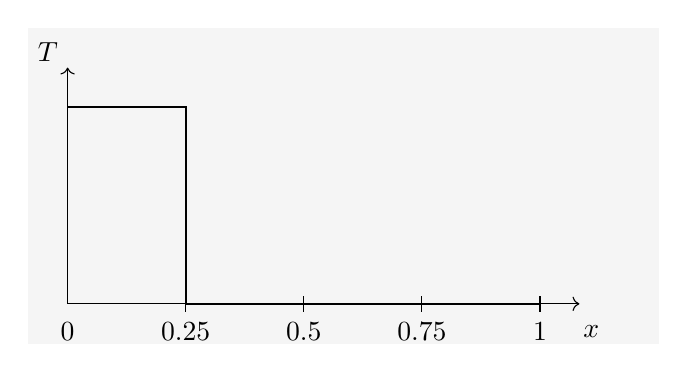
\begin{tikzpicture}
\draw[fill=gray!8,gray!8](0,0) rectangle (8,4);
%\draw[step=0.5cm,gray,very thin] (0,0) grid (8,4); %background grid

\draw[->] (0.5,0.5) -- (7,0.5) ; 
\node[] at (0.5,0.15) {$0$};

\node[] at (2,0.15) {$0.25$};
\node[] at (3.5,0.15) {$0.5$};
\node[] at (5,0.15) {$0.75$};
\node[] at (6.5,0.15) {$1$};
\draw[->] (0.5,0.5) -- (0.5,3.5) ; 
\node[] at (0.25,3.7) {$T$};


\draw[-] (2,0.4) -- (2,0.6) ; 
\draw[-] (3.5,0.4) -- (3.5,0.6) ; 
\draw[-] (5,0.4) -- (5,0.6) ; 
\draw[-] (6.5,0.4) -- (6.5,0.6) ; 


%\draw[-] (2,1) -- (1.75,0.75) ; 
%\draw[-] (2.5,1) -- (2.25,0.75) ; 
%\draw[-] (3,1) -- (2.75,0.75) ; 
%\draw[-] (3.5,1) -- (3.25,0.75) ; 
%\draw[-] (4,1) -- (3.75,0.75) ; 
%\draw[-] (4.5,1) -- (4.25,0.75) ; 

%---------------------------------

%\draw[thick,->] (7,1) -- (7,5) ; 
%\node[] at (6.6,4) {$L_y$};
%\node[] at (6.6,1) {$0$};
%\draw[-] (6.85,1) -- (7.15,1) ; 
%\draw[-] (6.85,4) -- (7.15,4) ; 
%\node[] at (7.6,4) {$p=0$};
%\node[] at (6.6,5) {$y$};

%---------------------------------

\draw[thick] (0.5,3) -- (2,3) -- (2,0.5) -- (6.5,0.5) ; 
\node[] at (7.15,0.15) {$x$};


\end{tikzpicture}



\end{center}

Program the above FTCS method. Run the model for 250 time steps with $\delta t=0.002$. 
Program the Lax-Friedrichs method by modifying the previous code.\\
Bonus: Program the upwind method and/or the Crank-Nicolson method. 

\par\noindent\rule{\textwidth}{0.4pt}
\end{minipage}
\end{center}
%-/-/-/-/-/-/-/-/-/-/-/-/-/-/-/-/-/-/




\newpage
\subsection{FDM basics in 2D} \label{ss:fdm_basics2D} 
In a 2D Cartesian domain overlain by a $nnx \times nny$ grid, 
the spacing between nodes in the $x$ and $y$ direction is $h_x$ 
and $h_y$ respectively. 

\begin{center}


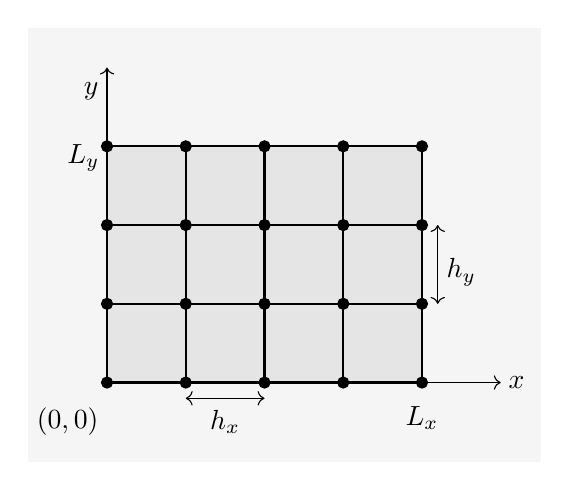
\begin{tikzpicture}
\draw[fill=gray!8,gray!8](0,0) rectangle (6.5,5.5);
%\draw[step=0.5cm,gray,very thin] (0,0) grid (8,5); %background grid


\draw[fill=gray!20,gray!20](1,1) rectangle (5,4);
\draw[thick] (1,1) -- (5,1) -- (5,4) -- (1,4) -- cycle;  

\draw[thick] (1,2) -- (5,2) ; 
\draw[thick] (1,3) -- (5,3) ; 
\draw[thick] (2,1) -- (2,4) ; 
\draw[thick] (3,1) -- (3,4) ; 
\draw[thick] (4,1) -- (4,4) ; 

\draw[black,fill=black] (1,1)  circle (2pt);
\draw[black,fill=black] (2,1)  circle (2pt);
\draw[black,fill=black] (3,1)  circle (2pt);
\draw[black,fill=black] (4,1)  circle (2pt);
\draw[black,fill=black] (5,1)  circle (2pt);
\draw[black,fill=black] (1,2)  circle (2pt);
\draw[black,fill=black] (2,2)  circle (2pt);
\draw[black,fill=black] (3,2)  circle (2pt);
\draw[black,fill=black] (4,2)  circle (2pt);
\draw[black,fill=black] (5,2)  circle (2pt);
\draw[black,fill=black] (1,3)  circle (2pt);
\draw[black,fill=black] (2,3)  circle (2pt);
\draw[black,fill=black] (3,3)  circle (2pt);
\draw[black,fill=black] (4,3)  circle (2pt);
\draw[black,fill=black] (5,3)  circle (2pt);
\draw[black,fill=black] (1,4)  circle (2pt);
\draw[black,fill=black] (2,4)  circle (2pt);
\draw[black,fill=black] (3,4)  circle (2pt);
\draw[black,fill=black] (4,4)  circle (2pt);
\draw[black,fill=black] (5,4)  circle (2pt);

\draw [<->] (5.2,2) -- (5.2,3); \node[] at (5.5,2.4) {$h_y$};
\draw [<->] (2,0.8) -- (3,0.8); \node[] at (2.5,0.5) {$h_x$};

\draw [->] (5,1) -- (6,1); \node[] at (6.2,1) {$x$};
\draw [->] (1,4) -- (1,5); \node[] at (0.8,4.7) {$y$};

\node[] at (0.5,0.5) {$(0,0)$};
\node[] at (5,0.55) {$L_x$};
\node[] at (0.7,3.85) {$L_y$};

%\node[] at (2.2,3.1) {\tiny{\color{brown}i-1,j}};
%\node[] at (3.2,3.1) {\tiny{\color{brown}i,j}};
%\node[] at (4.2,3.1) {\tiny{\color{brown}i+1,j}};

%\node[] at (3.2,4.1) {\tiny{\color{brown}i,j+1}};
%\node[] at (3.2,2.1) {\tiny{\color{brown}i,j-1}};

%\draw[black,fill=black] (3.1,0.2) circle (2pt); \node[] at (3.4,0.2) {$\vec\upnu$};
%\draw (4.1,0.2) circle (4pt); 
%\node[] at (2.5,4.5) {4 vel. nodes, 1 press. nodes};
\end{tikzpicture}

\end{center}

We have seen in Section~\ref{ss:fdm_basics1D} how to discretise second-order derivatives in 1D. 
In 2D, we then logically have for a function $f(x,y)$

\begin{equation}
\frac{\partial^2 f}{\partial x^2}(x_0,y_0) = \frac{f(x_0+h_x,y_0) -2f(x_0,y_0) + f(x_0-h_x,y_0) }{h_x^2} 
+ {\cal O}(h_x^2)
\end{equation}
\begin{equation}
\frac{\partial^2 f}{\partial y^2}(x_0,y_0) = \frac{f(x_0,y_0+h_y) -2f(x_0,y_0) + f(x_0,y_0-h_y) }{h_y^2} 
+ {\cal O}(h_y^2)
\end{equation}
What about mixed derivatives? Since these are combinations of first-order derivatives, 
we can straightforwardly discretise them:
\begin{eqnarray}
&& \frac{\partial^2 f }{\partial x \partial y}(x_0,y_0) \nn\\
&=& \frac{\partial }{\partial x} \left(\frac{\partial f}{\partial y}\right) (x_0,y_0) \nn\\
&=& \frac{\partial }{\partial x} \left(\frac{ f(x_0,y_0+h_y)-f(x_0,y_0-h_y)}{2h_y} \right) \nn\\
&=& \frac{1}{2h_y} \frac{\partial f}{\partial x} (x_0,y_0+h_y)
   -\frac{1}{2h_y} \frac{\partial f}{\partial x} (x_0,y_0-h_y) \nn\\
&=& \frac{1}{2h_y}  \frac{ f(x_0+h_x,y_0+h_y)-f(x_0-h_x,y_0+h_y)}{2h_x} 
-   \frac{1}{2h_y}  \frac{ f(x_0+h_x,y_0-h_y)-f(x_0-h_x,y_0-h_y)}{2h_x}  \nn\\
&=& \frac{f(x_0+h_x,y_0+h_y)-f(x_0-h_x,y_0+h_y)-f(x_0+h_x,y_0-h_y)+f(x_0-h_x,y_0-h_y)}{2 h_x h_y}
+ {\cal O}(h_x^2,h_y^2) \nn
\end{eqnarray}

%...............................
\subsubsection{From 1D to 2D}

INSERT TEXT

\begin{center}
\begin{flushright} {\tiny {\color{gray} (tikz\_needicon.tex)}} \end{flushright}
%~~~~~~~~~~~~~~~~~~~~~~~~~~~~~~~~~~~~~~~~~~~~~~~~~~~~~~~~~~~~~~~~~~~~~~~~~~~~~~~~~~~~~~~~~~~~~~~~~~


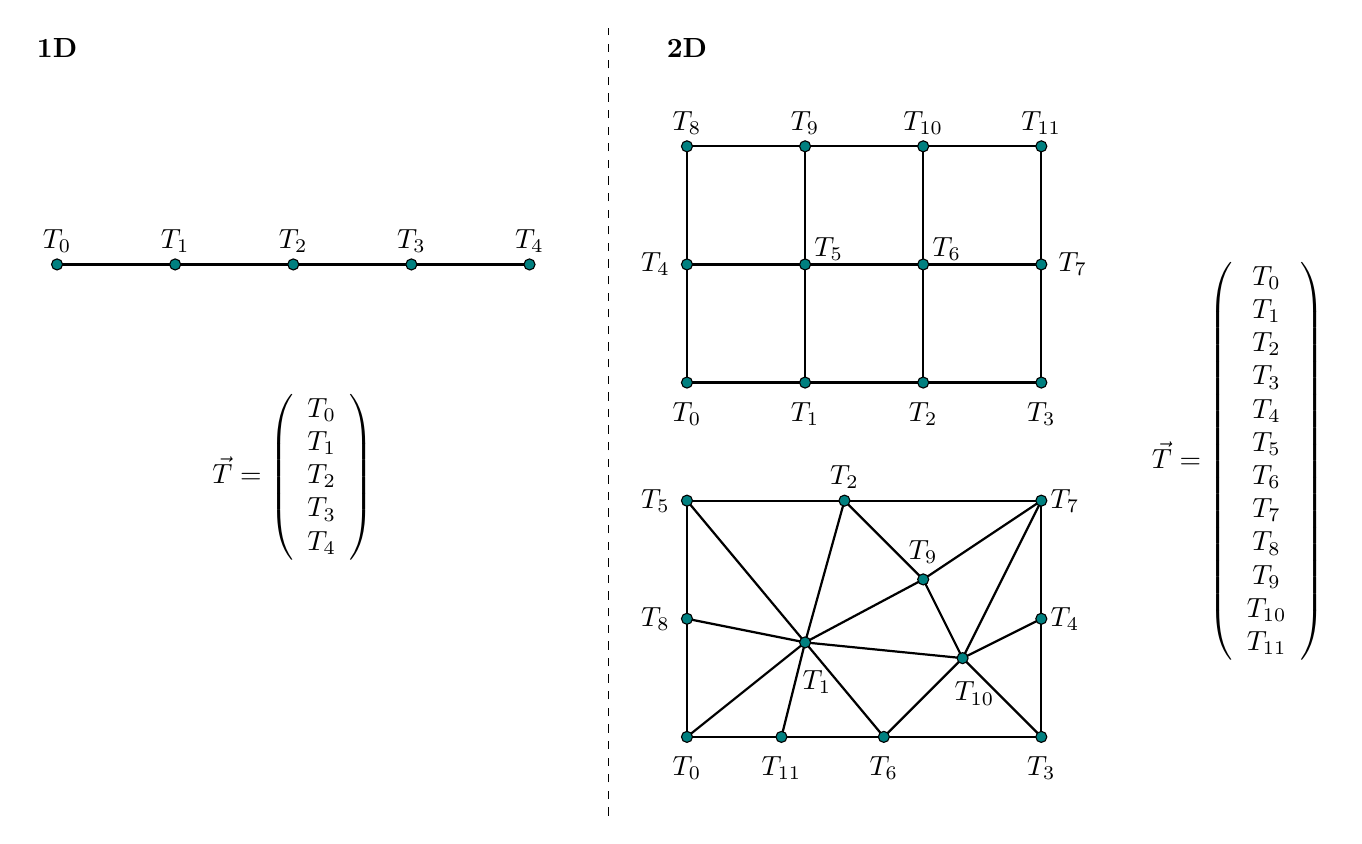
\begin{tikzpicture}
%\draw[step=0.5cm,gray,very thin] (0,0) grid (17,10); 

\node[] at (1,9.75) {\bf 1D};

\draw[thick] (1,7)--(7,7);
\draw[black,fill=teal] (1,7) circle (2pt);
\draw[black,fill=teal] (2.5,7) circle (2pt);
\draw[black,fill=teal] (4,7) circle (2pt);
\draw[black,fill=teal] (5.5,7) circle (2pt);
\draw[black,fill=teal] (7,7) circle (2pt);

\node[] at (1,7.3) {$T_0$};
\node[] at (2.5,7.3) {$T_1$};
\node[] at (4,7.3) {$T_2$};
\node[] at (5.5,7.3) {$T_3$};
\node[] at (7,7.3) {$T_4$};

\node[] at (4,4.3) {
$\vec{T}=\left(
\begin{array}{c}
T_0 \\ T_1 \\ T_2 \\ T_3 \\ T_4
\end{array}
\right)$};

%%%%%%%%%%%%%%%%%%%%%%%%%%%%%%%%%%%%%%%%%55
\draw[dashed] (8,0)--(8,10); 

\node[] at (9,9.75) {\bf 2D};

\draw[thick](9,5.5) rectangle (13.5,8.5);
\draw[thick](9,7)--(13.5,7);
\draw[thick](10.5,5.5)--(10.5,8.5);
\draw[thick](12,5.5)--(12,8.5);

\node[] at (16,4.5) {
$\vec{T}=\left(
\begin{array}{c}
T_0 \\ T_1 \\ T_2 \\ T_3 \\ T_4 \\
T_5 \\ T_6 \\ T_7 \\ T_8 \\ T_9 \\ T_{10} \\ T_{11}
\end{array}
\right)$};

\draw[black,fill=teal] (9,5.5) circle (2pt);
\draw[black,fill=teal] (10.5,5.5) circle (2pt);
\draw[black,fill=teal] (12,5.5) circle (2pt);
\draw[black,fill=teal] (13.5,5.5) circle (2pt);

\draw[black,fill=teal] (9,7) circle (2pt);
\draw[black,fill=teal] (10.5,7) circle (2pt);
\draw[black,fill=teal] (12,7) circle (2pt);
\draw[black,fill=teal] (13.5,7) circle (2pt);

\draw[black,fill=teal] (9,8.5) circle (2pt);
\draw[black,fill=teal] (10.5,8.5) circle (2pt);
\draw[black,fill=teal] (12,8.5) circle (2pt);
\draw[black,fill=teal] (13.5,8.5) circle (2pt);

\node[] at (9,5.1) {$T_0$};
\node[] at (10.5,5.1) {$T_1$};
\node[] at (12,5.1) {$T_2$};
\node[] at (13.5,5.1) {$T_3$};
\node[] at (8.6,7) {$T_4$};

\node[] at (10.8,7.2) {$T_5$};
\node[] at (12.3,7.2) {$T_6$};

\node[] at (13.9,7) {$T_7$};

\node[] at (9,8.8) {$T_8$};
\node[] at (10.5,8.8) {$T_9$};
\node[] at (12,8.8) {$T_{10}$};
\node[] at (13.5,8.8) {$T_{11}$};

%%%%%%%%%%%%%%%%%%%%%%%%%%%%%%%%%%%%%%%5
%triangular mesh

\draw[thick](9,1) rectangle (13.5,4);


\draw[thick](9,1)--(10.5,2.2)--(12,3)--(13.5,4);
\draw[thick](9,4)--(10.5,2.2)--(12.5,2)--(13.5,1);
\draw[thick](11,4)--(12,3)--(12.5,2)--(13.5,2.5);
\draw[thick](13.5,4)--(12.5,2)--(11.5,1)--(10.5,2.2)--(9,2.5);
\draw[thick](10.2,1)--(10.5,2.2)--(11,4);


\draw[black,fill=teal] (9,1) circle (2pt);
\draw[black,fill=teal] (10.2,1) circle (2pt);
\draw[black,fill=teal] (11.5,1) circle (2pt);
\draw[black,fill=teal] (13.5,1) circle (2pt);

\draw[black,fill=teal] (9,2.5) circle (2pt);
\draw[black,fill=teal] (10.5,2.2) circle (2pt);
\draw[black,fill=teal] (12,3) circle (2pt);
\draw[black,fill=teal] (12.5,2) circle (2pt);
\draw[black,fill=teal] (13.5,2.5) circle (2pt);

\draw[black,fill=teal] (9,4) circle (2pt);
\draw[black,fill=teal] (11,4) circle (2pt);
\draw[black,fill=teal] (13.5,4) circle (2pt);

\node[] at (9,0.6) {$T_0$};
\node[] at (10.2,0.6) {$T_{11}$};
\node[] at (11.5,0.6) {$T_6$};
\node[] at (13.5,0.6) {$T_3$};

\node[] at (8.6,2.5) {$T_8$};
\node[] at (8.6,4) {$T_5$};
\node[] at (11,4.3) {$T_2$};
\node[] at (13.8,4) {$T_7$};
\node[] at (13.8,2.5) {$T_4$};

\node[] at (12,3.35) {$T_9$};
\node[] at (12.65,1.55) {$T_{10}$};

\node[] at (10.65,1.7) {$T_1$};

\end{tikzpicture}

\end{center}


Also, here is a rather handy code snippet which should allow you to make nice plots of the coming exercises.

\begin{lstlisting}
       filename = 'solution_{:04d}.pdf'.format(istep) 
       fig = plt.figure ()
       ax = fig.gca(projection='3d')
       ax.plot_surface(x.reshape ((nny,nnx)),y.reshape((nny,nnx)),T.reshape((nny,nnx)),color = 'darkseagreen')
       ax.set_xlabel ( 'X [ m ] ')
       ax.set_ylabel ( 'Y [ m ] ')
       ax.set_zlabel ( ' Temperature  [ C ] ')
       plt.title('Timestep  %.2d' %(istep),loc='right')
       plt.grid ()
       plt.savefig(filename)
       #plt.show ()
       plt.close()
\end{lstlisting}

 
\newpage
\subsection{Solving the 2D diffusion equation} \label{ss:fdm_diff2D} We now revisit the transient heat equation, this time with sources/sinks for 2D problems.
The heat equation is 
\[
\rho C_p \frac{\partial T}{\partial t} =
\vec\nabla \cdot k \vec\nabla T + Q 
\]
which simply writes as follows when Cartesian coordinates are used:
\[
\rho C_p \frac{\partial T}{\partial t} = 
\frac{\partial }{\partial x} \left(  k  \frac{\partial T}{\partial x} \right)+
\frac{\partial }{\partial y} \left(  k  \frac{\partial T}{\partial y} \right)+
Q
\]
where $Q$ is the radiogenic heat production.

If the heat conductivity is constant, it writes:
\[
\frac{\partial T}{\partial t} =
\kappa \left(  \frac{\partial^2 T}{\partial x^2} +   \frac{\partial^2 T}{\partial y^2} \right)+
\frac{Q}{\rho C_p}
\]

In order to solve this equation over the Cartesian domain of size $L_x \times L_y$
we need to generate a mesh as shown hereunder:
\begin{center}
\includegraphics[width=8cm]{images/fdm/fdgrid}
\end{center}
The spacing between the nodes in the $x$-direction is $h_x$ and $h_y$ is the spacing
between the nodes in the vertical direction. There are now $np=nnx\times nny$ nodes in total.

In one dimension, the subscript indicated the node $i$. In two dimensions we therefore 
need two indices ${\color{brown}i}$ and ${\color{brown}j}$ 
to identify a node, so that the temperature at node ${\color{brown}i},{\color{brown}j}$ 
at time $n$ is denoted $T_{{\color{brown}i,j}}^n$.

%The vector $\vec{T}$ contains all the temperature unknowns, so it is a vector that is $np$-long. 
%But how should this vector be organised ? In other words, 
One question remains: should we number nodes 
row by row ? column by column ? randomly ? 
These three approaches are shown hereunder: 

\vspace{.5cm}

\begin{minipage}[t]{\textwidth}


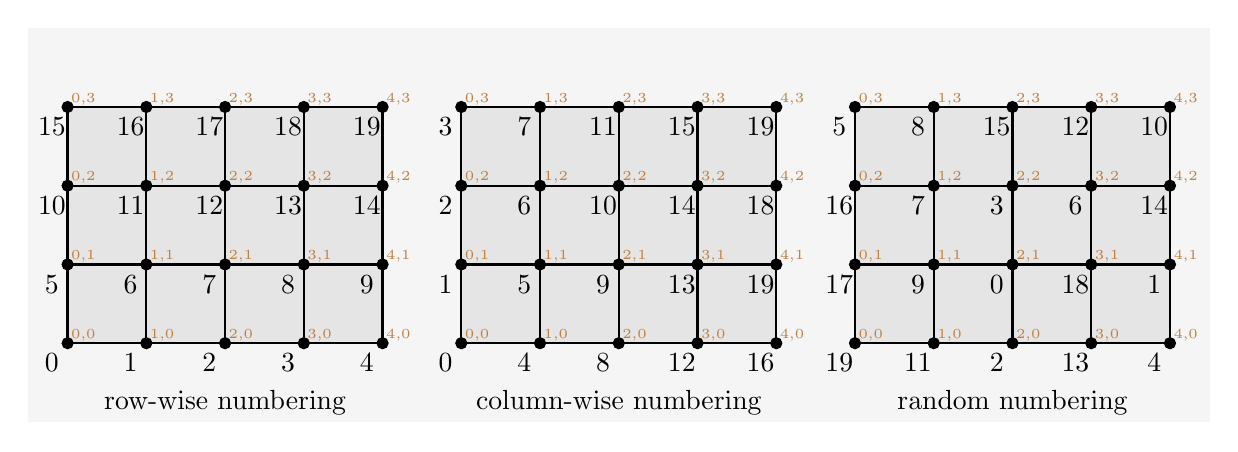
\begin{tikzpicture}
\draw[fill=gray!8,gray!8](0.5,0) rectangle (15.5,5);
%\draw[step=0.5cm,gray,very thin] (0,0) grid (17,5); %background grid

\draw[fill=gray!20,gray!20](1,1) rectangle (5,4);
\draw[fill=gray!20,gray!20](6,1) rectangle (10,4);
\draw[fill=gray!20,gray!20](11,1) rectangle (15,4);

\draw[thick] (1,1) -- (5,1) -- (5,4) -- (1,4) -- cycle;  
\draw[thick] (1,2) -- (5,2) ; 
\draw[thick] (1,3) -- (5,3) ; 
\draw[thick] (2,1) -- (2,4) ; 
\draw[thick] (3,1) -- (3,4) ; 
\draw[thick] (4,1) -- (4,4) ; 
\node[] at (0.8,0.75) {0};
\node[] at (1.8,0.75) {1};
\node[] at (2.8,0.75) {2};
\node[] at (3.8,0.75) {3};
\node[] at (4.8,0.75) {4};
\node[] at (0.8,1.75) {5};
\node[] at (1.8,1.75) {6};
\node[] at (2.8,1.75) {7};
\node[] at (3.8,1.75) {8};
\node[] at (4.8,1.75) {9};
\node[] at (0.8,2.75) {10};
\node[] at (1.8,2.75) {11};
\node[] at (2.8,2.75) {12};
\node[] at (3.8,2.75) {13};
\node[] at (4.8,2.75) {14};
\node[] at (0.8,3.75) {15};
\node[] at (1.8,3.75) {16};
\node[] at (2.8,3.75) {17};
\node[] at (3.8,3.75) {18};
\node[] at (4.8,3.75) {19};
\node[] at (1.2,1.1) {\tiny{\color{brown} 0,0}};
\node[] at (2.2,1.1) {\tiny{\color{brown} 1,0}};
\node[] at (3.2,1.1) {\tiny{\color{brown} 2,0}};
\node[] at (4.2,1.1) {\tiny{\color{brown} 3,0}};
\node[] at (5.2,1.1) {\tiny{\color{brown} 4,0}};
\node[] at (1.2,2.1) {\tiny{\color{brown} 0,1}};
\node[] at (2.2,2.1) {\tiny{\color{brown} 1,1}};
\node[] at (3.2,2.1) {\tiny{\color{brown} 2,1}};
\node[] at (4.2,2.1) {\tiny{\color{brown} 3,1}};
\node[] at (5.2,2.1) {\tiny{\color{brown} 4,1}};
\node[] at (1.2,3.1) {\tiny{\color{brown} 0,2}};
\node[] at (2.2,3.1) {\tiny{\color{brown} 1,2}};
\node[] at (3.2,3.1) {\tiny{\color{brown} 2,2}};
\node[] at (4.2,3.1) {\tiny{\color{brown} 3,2}};
\node[] at (5.2,3.1) {\tiny{\color{brown} 4,2}};
\node[] at (1.2,4.1) {\tiny{\color{brown} 0,3}};
\node[] at (2.2,4.1) {\tiny{\color{brown} 1,3}};
\node[] at (3.2,4.1) {\tiny{\color{brown} 2,3}};
\node[] at (4.2,4.1) {\tiny{\color{brown} 3,3}};
\node[] at (5.2,4.1) {\tiny{\color{brown} 4,3}};
\draw[black,fill=black] (1,1)  circle (2pt);
\draw[black,fill=black] (2,1)  circle (2pt);
\draw[black,fill=black] (3,1)  circle (2pt);
\draw[black,fill=black] (4,1)  circle (2pt);
\draw[black,fill=black] (5,1)  circle (2pt);
\draw[black,fill=black] (1,2)  circle (2pt);
\draw[black,fill=black] (2,2)  circle (2pt);
\draw[black,fill=black] (3,2)  circle (2pt);
\draw[black,fill=black] (4,2)  circle (2pt);
\draw[black,fill=black] (5,2)  circle (2pt);
\draw[black,fill=black] (1,3)  circle (2pt);
\draw[black,fill=black] (2,3)  circle (2pt);
\draw[black,fill=black] (3,3)  circle (2pt);
\draw[black,fill=black] (4,3)  circle (2pt);
\draw[black,fill=black] (5,3)  circle (2pt);
\draw[black,fill=black] (1,4)  circle (2pt);
\draw[black,fill=black] (2,4)  circle (2pt);
\draw[black,fill=black] (3,4)  circle (2pt);
\draw[black,fill=black] (4,4)  circle (2pt);
\draw[black,fill=black] (5,4)  circle (2pt);
%---------------------------------------------------
\draw[thick] (6,1) -- (10,1) -- (10,4) -- (6,4) -- cycle;  
\draw[thick] (6,2) -- (10,2) ; 
\draw[thick] (6,3) -- (10,3) ; 
\draw[thick] (7,1) -- (7,4) ; 
\draw[thick] (8,1) -- (8,4) ; 
\draw[thick] (9,1) -- (9,4) ; 
\node[] at (6.2,1.1)  {\tiny{\color{brown} 0,0}};
\node[] at (7.2,1.1)  {\tiny{\color{brown} 1,0}};
\node[] at (8.2,1.1)  {\tiny{\color{brown} 2,0}};
\node[] at (9.2,1.1)  {\tiny{\color{brown} 3,0}};
\node[] at (10.2,1.1) {\tiny{\color{brown} 4,0}};
\node[] at (6.2,2.1)  {\tiny{\color{brown} 0,1}};
\node[] at (7.2,2.1)  {\tiny{\color{brown} 1,1}};
\node[] at (8.2,2.1)  {\tiny{\color{brown} 2,1}};
\node[] at (9.2,2.1)  {\tiny{\color{brown} 3,1}};
\node[] at (10.2,2.1) {\tiny{\color{brown} 4,1}};
\node[] at (6.2,3.1)  {\tiny{\color{brown} 0,2}};
\node[] at (7.2,3.1)  {\tiny{\color{brown} 1,2}};
\node[] at (8.2,3.1)  {\tiny{\color{brown} 2,2}};
\node[] at (9.2,3.1)  {\tiny{\color{brown} 3,2}};
\node[] at (10.2,3.1) {\tiny{\color{brown} 4,2}};
\node[] at (6.2,4.1)  {\tiny{\color{brown} 0,3}};
\node[] at (7.2,4.1)  {\tiny{\color{brown} 1,3}};
\node[] at (8.2,4.1)  {\tiny{\color{brown} 2,3}};
\node[] at (9.2,4.1)  {\tiny{\color{brown} 3,3}};
\node[] at (10.2,4.1) {\tiny{\color{brown} 4,3}};
\draw[black,fill=black] (6,1)  circle (2pt);
\draw[black,fill=black] (7,1)  circle (2pt);
\draw[black,fill=black] (8,1)  circle (2pt);
\draw[black,fill=black] (9,1)  circle (2pt);
\draw[black,fill=black] (10,1)  circle (2pt);
\draw[black,fill=black] (6,2)  circle (2pt);
\draw[black,fill=black] (7,2)  circle (2pt);
\draw[black,fill=black] (8,2)  circle (2pt);
\draw[black,fill=black] (9,2)  circle (2pt);
\draw[black,fill=black] (10,2)  circle (2pt);
\draw[black,fill=black] (6,3)  circle (2pt);
\draw[black,fill=black] (7,3)  circle (2pt);
\draw[black,fill=black] (8,3)  circle (2pt);
\draw[black,fill=black] (9,3)  circle (2pt);
\draw[black,fill=black] (10,3)  circle (2pt);
\draw[black,fill=black] (6,4)  circle (2pt);
\draw[black,fill=black] (7,4)  circle (2pt);
\draw[black,fill=black] (8,4)  circle (2pt);
\draw[black,fill=black] (9,4)  circle (2pt);
\draw[black,fill=black] (10,4)  circle (2pt);
\node[] at (5.8,0.75) {0};
\node[] at (6.8,0.75) {4};
\node[] at (7.8,0.75) {8};
\node[] at (8.8,0.75) {12};
\node[] at (9.8,0.75) {16};
\node[] at (5.8,1.75) {1};
\node[] at (6.8,1.75) {5};
\node[] at (7.8,1.75) {9};
\node[] at (8.8,1.75) {13};
\node[] at (9.8,1.75) {19};
\node[] at (5.8,2.75) {2};
\node[] at (6.8,2.75) {6};
\node[] at (7.8,2.75) {10};
\node[] at (8.8,2.75) {14};
\node[] at (9.8,2.75) {18};
\node[] at (5.8,3.75) {3};
\node[] at (6.8,3.75) {7};
\node[] at (7.8,3.75) {11};
\node[] at (8.8,3.75) {15};
\node[] at (9.8,3.75) {19};

%---------------------------------------------------
\draw[thick] (11,1) -- (15,1) -- (15,4) -- (11,4) -- cycle;  
\draw[thick] (11,2) -- (15,2) ; 
\draw[thick] (11,3) -- (15,3) ; 
\draw[thick] (12,1) -- (12,4) ; 
\draw[thick] (13,1) -- (13,4) ; 
\draw[thick] (14,1) -- (14,4) ; 
\node[] at (11.2,1.1) {\tiny{\color{brown} 0,0}};
\node[] at (12.2,1.1) {\tiny{\color{brown} 1,0}};
\node[] at (13.2,1.1) {\tiny{\color{brown} 2,0}};
\node[] at (14.2,1.1) {\tiny{\color{brown} 3,0}};
\node[] at (15.2,1.1) {\tiny{\color{brown} 4,0}};
\node[] at (11.2,2.1) {\tiny{\color{brown} 0,1}};
\node[] at (12.2,2.1) {\tiny{\color{brown} 1,1}};
\node[] at (13.2,2.1) {\tiny{\color{brown} 2,1}};
\node[] at (14.2,2.1) {\tiny{\color{brown} 3,1}};
\node[] at (15.2,2.1) {\tiny{\color{brown} 4,1}};
\node[] at (11.2,3.1) {\tiny{\color{brown} 0,2}};
\node[] at (12.2,3.1) {\tiny{\color{brown} 1,2}};
\node[] at (13.2,3.1) {\tiny{\color{brown} 2,2}};
\node[] at (14.2,3.1) {\tiny{\color{brown} 3,2}};
\node[] at (15.2,3.1) {\tiny{\color{brown} 4,2}};
\node[] at (11.2,4.1) {\tiny{\color{brown} 0,3}};
\node[] at (12.2,4.1) {\tiny{\color{brown} 1,3}};
\node[] at (13.2,4.1) {\tiny{\color{brown} 2,3}};
\node[] at (14.2,4.1) {\tiny{\color{brown} 3,3}};
\node[] at (15.2,4.1) {\tiny{\color{brown} 4,3}};
\draw[black,fill=black] (11,1)  circle (2pt);
\draw[black,fill=black] (12,1)  circle (2pt);
\draw[black,fill=black] (13,1)  circle (2pt);
\draw[black,fill=black] (14,1)  circle (2pt);
\draw[black,fill=black] (15,1)  circle (2pt);
\draw[black,fill=black] (11,2)  circle (2pt);
\draw[black,fill=black] (12,2)  circle (2pt);
\draw[black,fill=black] (13,2)  circle (2pt);
\draw[black,fill=black] (14,2)  circle (2pt);
\draw[black,fill=black] (15,2)  circle (2pt);
\draw[black,fill=black] (11,3)  circle (2pt);
\draw[black,fill=black] (12,3)  circle (2pt);
\draw[black,fill=black] (13,3)  circle (2pt);
\draw[black,fill=black] (14,3)  circle (2pt);
\draw[black,fill=black] (15,3)  circle (2pt);
\draw[black,fill=black] (11,4)  circle (2pt);
\draw[black,fill=black] (12,4)  circle (2pt);
\draw[black,fill=black] (13,4)  circle (2pt);
\draw[black,fill=black] (14,4)  circle (2pt);
\draw[black,fill=black] (15,4)  circle (2pt);
\node[] at (10.8,0.75) {19};
\node[] at (11.8,0.75) {11};
\node[] at (12.8,0.75) {2};
\node[] at (13.8,0.75) {13};
\node[] at (14.8,0.75) {4};
\node[] at (10.8,1.75) {17};
\node[] at (11.8,1.75) {9};
\node[] at (12.8,1.75) {0};
\node[] at (13.8,1.75) {18};
\node[] at (14.8,1.75) {1};
\node[] at (10.8,2.75) {16};
\node[] at (11.8,2.75) {7};
\node[] at (12.8,2.75) {3};
\node[] at (13.8,2.75) {6};
\node[] at (14.8,2.75) {14};
\node[] at (10.8,3.75) {5};
\node[] at (11.8,3.75) {8};
\node[] at (12.8,3.75) {15};
\node[] at (13.8,3.75) {12};
\node[] at (14.8,3.75) {10};


\node[] at (3,0.25) {row-wise numbering};
\node[] at (8,0.25) {column-wise numbering};
\node[] at (13,0.25) {random numbering};

\end{tikzpicture}
\\
\begin{center}
{\captionfont Left: row-wise numbering; middle: column-wise ordering; Right: random numbering.
$nnx=5$, $nny=4$ and therefore $np=20$.
}
\end{center}
\end{minipage}

\vspace{.5cm}

This is a critical point because the discretised PDE is formulated as a function of $T_{{\color{brown} i,j}}$ 
with ${\color{brown}i}=0,\dot nnx-1$ and ${\color{brown}j}=0,\dots nny-1$ 
but the vector $\vec{T}$ containing all these values
is indexed by a single index ${\color{teal}k}=0,\dots np-1$. The numbering strategy determines how easy
it is to go from $({\color{brown}i},{\color{brown}j})$ to ${\color{teal}k}$ and vice versa. 
Very concretely again, where does $T_{\color{brown}3,4}$ should be placed in the global 
vector of unknowns $\vec{T}$?

We then need a (preferably simple/straightforward) 'function' 
which associates to every $(i,j)$ a global index $k$. 
For the first grid with row-wise numbering, we have 
$0\leq {\color{brown}i} \leq 4$ , $0 \leq {\color{brown}j} \leq 3$ 
so that $0 \leq {\color{teal}k} \leq 19$
and it follows that 
\[
{\color{teal} k}={\color{brown}j}*nnx+{\color{brown}i}
\]
This is easy to verify: ${\color{brown}i}=3$ and ${\color{brown}j}=2$ 
does correspond to the $13^{th} node$, 
${\color{brown}i}=4$ and ${\color{brown}j}=1$ does correspond to the $9^{th} node$, etc ...

\begin{minipage}[t]{\textwidth}
\begin{center}
\input{tikz_fdm5x4mesh}
\end{center}
\end{minipage}







%.............................
\paragraph{Explicit scheme} The simplest approach is an {\color{olive} FTCS} 
(forward time, centered space) explicit method like in 1D:
\[
\frac{T_{{\color{brown}i,j}}^{n+1}-T_{{\color{brown}i,j}}^n}{\delta t}
= \kappa
\left(
\frac{ T_{{\color{brown}i-1,j}}^{n}-2T_{{\color{brown}i,j}}^{n}+T_{{\color{brown}i+1,j}}^{n}  }{h_x^2} + 
\frac{ T_{{\color{brown}i,j-1}}^{n}-2T_{{\color{brown}i,j}}^{n}+T_{{\color{brown}i,j+1}}^{n}  }{h_y^2}
\right)
+\frac{Q_{{\color{brown}i,j}}^n}{\rho C_p}
\]
where we have assumed that the source term $Q$ can depend of space coordinates and therefore 
appears as $Q_{i,j}$ in the equation.
We define $s_x$ and $s_y$ as follows:
\[
s_x = \frac{\kappa \delta t}{h_x^2}
\quad\quad
s_y = \frac{\kappa \delta t}{h_y^2}
\]
so that
\[
T_{{\color{brown}i,j}}^{n+1} = T_{{\color{brown}i,j}}^n 
+ s_x ( T_{{\color{brown}i-1,j}}^{n}
-2T_{{\color{brown}i,j}}^{n}+T_{i+1,j}^{n} ) 
+s_y ( T_{{\color{brown}i,j-1}}^{n}
-2T_{{\color{brown}i,j}}^{n}
+T_{{\color{brown}i,j+1}}^{n} ) + 
\frac{Q_{{\color{brown}i,j}}^n \delta t}{\rho C_p}
\]
The scheme is stable for  
\[
\delta t \leq \frac{\min(h_x^2,h_y^2)}{2 \kappa}
\]
Boundary conditions can be set the usual way. A constant (Dirichlet) temperature 
at node $(i,j)$ is given by
\[
T_{i,j}=T_{bc} 
\]
where $T_{bc}$ is the prescribed temperature. 

%...........................
\paragraph{Implicit scheme} 
If we now employ a fully implicit, unconditionally stable discretization scheme, the discretised 
PDE becomes:
\[
\frac{T_{i,j}^{n+1}-T_{i,j}^n}{\delta t}
= \kappa
\left(
\frac{ T_{i-1,j}^{n+1}-2T_{i,j}^{n+1}+T_{i+1,j}^{n+1}  }{h_x^2} + 
\frac{ T_{i,j-1}^{n+1}-2T_{i,j}^{n+1}+T_{i,j+1}^{n+1}  }{h_y^2}
\right)
+\frac{Q_{i,j}^n}{\rho C_p}
\]

Rearranging terms with $n+1$ on the left and terms with $n$ on the right hand side gives
\[
-s_x T_{i+1,j}^{n+1}-s_y T_{i,j+1}^{n+1} +(1+2s_x+2s_y)T_{i,j}^{n+1} -s_x T_{i-1,j}^{n+1} -s_y T_{i,j-1}^{n+1} 
=
T_{i,j}^n
+\frac{Q_{i,j}^n \delta t}{\rho C_p}
\]
which here again yields a linear system of equations written ${\bm A}\cdot {\vec T} = {\vec b}$
where ${\bm A}$ is a $(np \times np)$ matrix.



Boundary conditions are $T(x,y)=0$ on all sides, so all nodes 
on the boundary have a prescribed zero temperature\footnote{We assume
here again that these boundary conditions do not change with time.}:
\begin{eqnarray}
T_{\color{brown}0,0} = T_{\color{teal} 0} &=& 0 \nn\\
T_{\color{brown}1,0} = T_{\color{teal} 1} &=& 0 \nn\\
T_{\color{brown}2,0} = T_{\color{teal} 2} &=& 0 \nn\\
T_{\color{brown}3,0} = T_{\color{teal} 3} &=& 0 \nn\\
T_{\color{brown}4,0} = T_{\color{teal} 4} &=& 0 \nn\\
T_{\color{brown}0,1} = T_{\color{teal} 5} &=& 0 \nn\\
T_{\color{brown}4,1} = T_{\color{teal} 9} &=& 0 \nn\\
T_{\color{brown}0,2} = T_{\color{teal} 10} &=& 0 \nn\\
T_{\color{brown}4,2} = T_{\color{teal} 14} &=& 0 \nn\\
T_{\color{brown}0,3} = T_{\color{teal} 15} &=& 0 \nn\\
T_{\color{brown}1,3} = T_{\color{teal} 16} &=& 0 \nn\\
T_{\color{brown}2,3} = T_{\color{teal} 17} &=& 0 \nn\\
T_{\color{brown}3,3} = T_{\color{teal} 18} &=& 0 \nn\\
T_{\color{brown}4,3} = T_{\color{teal} 19} &=& 0 \nn
\end{eqnarray}
In what follows we assume for simplicity and conciseness of notation that 
$h_x=h_y=h$ so that $s_x=s_y=s$ and we will use the notationa $\tilde{Q}=Q \delta t/\rho C_p$
The discretised PDE equation will now be applied to the interior nodes:
\[
-s T_{{\color{brown} i+1,j}}^{n+1}
-s T_{{\color{brown}i,j+1}}^{n+1} 
+(1+4s)T_{{\color{brown}i,j}}^{n+1} 
-s T_{{\color{brown}i-1,j}}^{n+1} 
-s T_{{\color{brown}i,j-1}}^{n+1} 
= T_{{\color{brown}i,j}}^n 
+\tilde{Q}_{{\color{brown}i,j}}^n
\]

\begin{itemize}
\item For node ${\color{teal}k}=6$ (${\color{brown}i}=1,{\color{brown}j}=1$):
\[
-s T_{{\color{brown}2,1}}^{n+1}
-s T_{{\color{brown}1,2}}^{n+1} 
+(1+4s)T_{{\color{brown}1,1}}^{n+1} 
-s T_{{\color{brown}0,1}}^{n+1} 
-s T_{{\color{brown}1,0}}^{n+1} 
= T_{{\color{brown}1,1}}^n +\tilde{Q}_{{\color{brown}1,1}}^n
\]
or, 
\[
-s T_{\color{teal} 7}^{n+1}-s T_{\color{teal} 11}^{n+1} +(1+4s)T_{\color{teal} 6}^{n+1} -s T_{\color{teal} 5}^{n+1} -s T_{\color{teal} 1}^{n+1} 
= T_{\color{teal} 6}^n +\tilde{Q}_{\color{teal} 6}^n
\]

\item For node $k=7$ ($i=2,j=1$):
\item For node $k=8$ ($i=3,j=1$):
\item For node $k=11$ ($i=1,j=2$):
\item For node $k=12$ ($i=2,j=2$):
\item For node $k=13$ ($i=3,j=2$):
\end{itemize}



\begin{landscape}
\[
\left(
\begin{array}{cccccccccccccccccccc}
1 & . & . & . & . & . & . & . & . & . & . & . & . & . & . & . & . & . & . & . \\ %#0
. & 1 & . & . & . & . & . & . & . & . & . & . & . & . & . & . & . & . & . & . \\ %#1
. & . & 1 & . & . & . & . & . & . & . & . & . & . & . & . & . & . & . & . & . \\ %#2
. & . & . & 1 & . & . & . & . & . & . & . & . & . & . & . & . & . & . & . & . \\ %#3
. & . & . & . & 1 & . & . & . & . & . & . & . & . & . & . & . & . & . & . & . \\ %#4
. & . & . & . & . & 1 & . & . & . & . & . & . & . & . & . & . & . & . & . & . \\ %#5
. & -s& . & . & . & -s& {1+4s} & -s& . & . & . & -s & . & . & . & . & . & . & . & . \\ %#6
. & . & -s& . & . & . & -s& {1+4s} & -s& . & . & . & -s & . & . & . & . & . & . & .\\ %#7
. & . & . & -s& . & . & . & -s & {1+4s} & -s & . & . & . & -s & . & . & . & . & . & . \\ %#8
. & . & . & . & . & . & . & . & . & 1 & . & . & . & . & . & . & . & . & . & . \\ %#9
. & . & . & . & . & . & . & . & . & . & 1 & . & . & . & . & . & . & . & . & . \\ %#10
. & . & . & . & . & . &-s & . & . & . & -s& {1+4s} & -s& . & . & .  & -s& . & . & .\\ %#11
. & . & . & . & . & . & . &-s & . & . & . & -s& {1+4s} & -s& . & . & .  & -s& . & .\\ %#12
. & . & . & . & . & . & . & . &-s & . & . & . & -s& {1+4s} & -s& . & . & .  & -s & .\\ %#13
. & . & . & . & . & . & . & . & . & . & . & . & . & . & 1 & . & . & . & . & . \\ %#14
. & . & . & . & . & . & . & . & . & . & . & . & . & . & . & 1 & . & . & . & . \\ %#15
. & . & . & . & . & . & . & . & . & . & . & . & . & . & . & . & 1 & . & . & . \\ %#16
. & . & . & . & . & . & . & . & . & . & . & . & . & . & . & . & . & 1 & . & . \\ %#17
. & . & . & . & . & . & . & . & . & . & . & . & . & . & . & . & . & . & 1 & . \\ %#18
. & . & . & . & . & . & . & . & . & . & . & . & . & . & . & . & . & . & . & 1    %#19
\end{array}
\right)
\cdot
\underbrace{
\left(
\begin{array}{c}
T_{\color{teal}0} \\ 
T_{\color{teal}1} \\ 
T_{\color{teal}2} \\ 
T_{\color{teal}3} \\ 
T_{\color{teal}4} \\ 
T_{\color{teal}5} \\ 
T_{\color{teal}6} \\ 
T_{\color{teal}7} \\ 
T_{\color{teal}8} \\ 
T_{\color{teal}9} \\ 
T_{\color{teal}10} \\ 
T_{\color{teal}11} \\ 
T_{\color{teal}12} \\ 
T_{\color{teal}13} \\ 
T_{\color{teal}14} \\ 
T_{\color{teal}15} \\ 
T_{\color{teal}16} \\ 
T_{\color{teal}17} \\ 
T_{\color{teal}18} \\ 
T_{\color{teal}19} 
\end{array}
\right)
}_{\vec T}
=
\underbrace{
\left(
\begin{array}{c}
0\\ 
0\\ 
0\\ 
0\\ 
0\\ 
0\\ 
T_{{\color{teal}6}}^n + \tilde{Q}_{\color{teal}6} \\ 
T_{{\color{teal}7}}^n + \tilde{Q}_{\color{teal}7} \\ 
T_{{\color{teal}8}}^n + \tilde{Q}_{\color{teal}8} \\ 
0\\ 
0\\ 
T_{{\color{teal}11}}^n + \tilde{Q}_{\color{teal}11} \\ 
T_{{\color{teal}12}}^n + \tilde{Q}_{\color{teal}12} \\ 
T_{{\color{teal}13}}^n + \tilde{Q}_{\color{teal}13} \\ 
0\\ 
0\\ 
0\\ 
0\\ 
0\\ 
0 
\end{array}
\right)
}_{\vec b}
\]
\end{landscape}


Note that we now have five diagonals filled with non-zero entries as opposed to three
diagonals in the 1D case.






\subsection{Solving the 2D advection-diffusion equation} \label{ss:fdm_advdiff2D} 
So far, we have mainly focused on the diffusion equation in a non-moving domain 
(relevant for the case of a dike intrusion cooling off 
or for a lithosphere which remains undeformed). 

We now want to consider problems where material moves during the time period under 
consideration and takes temperature anomalies with it (e.g. a plume rising 
through a convecting mantle). 
If the numerical grid remains fixed in the background, the hot temperatures should 
be moved to different grid points at each time step. 

We start again from the heat transport equation of Section~\ref{ss:hte}:
\begin{equation}
\rho C_p \left( \frac{\partial T}{\partial t} + \vec\upnu \cdot \vec\nabla T  \right)=
\vec\nabla \cdot k \vec\nabla T + Q 
\end{equation}
In one-dimensional Cartesian coordinates:
\begin{equation}
\rho C_p \left( \frac{\partial T}{\partial t}  
+ u \frac{\partial T}{\partial x} \right)= 
\frac{\partial }{\partial x} \left(  k  \frac{\partial T}{\partial x} \right)+ Q
\end{equation}
and in 2D
\begin{equation}
\rho C_p \left( \frac{\partial T}{\partial t}   
+ u \frac{\partial T}{\partial x}  
+ v \frac{\partial T}{\partial y} \right) 
=
\frac{\partial }{\partial x} \left(  k  \frac{\partial T}{\partial x} \right)
+
\frac{\partial }{\partial y} \left(  k  \frac{\partial T}{\partial y} \right)
+Q
\end{equation}
and in the case where $k$ is constant in space:
\begin{equation}
\frac{\partial T}{\partial t}   
+ u \frac{\partial T}{\partial x}  
+ v \frac{\partial T}{\partial y} 
=
\kappa \left( 
\frac{\partial^2 T}{\partial x^2} 
+ \frac{\partial^2 T}{\partial y^2} \right) +Q
\end{equation}
Since we have already seen how to deal with 'pure' diffusion equations in the 
previous section, let us now turn to 'pure' advection equations:

\begin{equation}
\frac{\partial T}{\partial t}  + u \frac{\partial T}{\partial x} = 0
\end{equation}
or
\begin{equation}
\frac{\partial T}{\partial t}  + u \frac{\partial T}{\partial x} + v \frac{\partial T}{\partial y}= 0
\end{equation}
where we assume $\vec\upnu=(u,v)$ known. 

Even though the equations appear simple, it is quite tricky to solve them accurately, 
more so than for the diffusion problem. 
This is particularly the case if there are large gradients in the quantity that is to be advected. 







\newpage
\subsection{FEM vs FDM?}\label{ss:femvsfdm}   
Let us start with the 1D steady advection-diffusion equation:
\begin{equation}
\rho C_p u \frac{dT}{dx} - k \frac{d^2T}{dx^2} = f \qquad \text{in} \quad [0,L_x]
\label{eq:fdm1Dad}
\end{equation}
with the boundary conditions $T(x=0)=0$ and $T(x=L_x)=0$.

We have seen before (see Section~\ref{XXX}) 
that the elemental matrix ${\bm K}_a$ for the advection and 
the elemental matrix  ${\bm K}_d$ for the diffusion terms are
\[
{\bm K}_a^e = \frac{\rho C_p u}{2} 
\left(
\begin{array}{cc}
-1 & 1 \\
-1 & 1 
\end{array}
\right)
\qquad
{\bm K}_d^e=\frac{k}{h_x}
\left(
\begin{array}{cc}
1 & -1 \\ 
-1 & 1
\end{array}
\right)
\]
where $h_x$ is the distance between nodes in the $x$-direction 
and $e$ denotes the element number. 

Assuming that we have 5 elements (i.e. 6 nodes), the assembled $6\times 6$ 
advection and diffusion matrices 
(before boundary conditions are applied) are:
\[
{\bm K}_a
= \frac{\rho C_p u}{2}
\left(
\begin{array}{cccccc}
-1 & 1 & 0 & 0 & 0  &0\\
-1 & 0 & 1 & 0 & 0  &0\\
 0 &-1 & 0 & 1 & 0  &0\\
 0 & 0 &-1 & 0 & 1  &0\\
 0 & 0 & 0 &-1 & 0  &1\\
 0 & 0 & 0 & 0 &-1  &1\\
\end{array}
\right)
\qquad
{\bm K}_d
= \frac{k}{h_x}
\left(
\begin{array}{cccccc}
 1 &-1 & 0 & 0 & 0 &  0\\
-1 & 2 &-1 & 0 & 0 &  0\\
 0 &-1 & 2 &-1 & 0 &  0\\
 0 & 0 &-1 & 2 &-1 &  0\\
 0 & 0 & 0 &-1 & 2 & -1\\
 0 & 0 & 0 & 0 &-1 &  1\\
\end{array}
\right)
\]
The rhs is zero, so that we would have to solve $({\bm K}_a+{\bm K}_d)\cdot \vec{T}=0$ 
, or:
\[
\left[ 
\frac{\rho C_p u}{2}
\left(
\begin{array}{cccccc}
-1 & 1 & 0 & 0 & 0  &0\\
-1 & 0 & 1 & 0 & 0  &0\\
 0 &-1 & 0 & 1 & 0  &0\\
 0 & 0 &-1 & 0 & 1  &0\\
 0 & 0 & 0 &-1 & 0  &1\\
 0 & 0 & 0 & 0 &-1  &1\\
\end{array}
\right)
+
\frac{k}{h_x}
\left(
\begin{array}{cccccc}
 1 &-1 & 0 & 0 & 0 &  0\\
-1 & 2 &-1 & 0 & 0 &  0\\
 0 &-1 & 2 &-1 & 0 &  0\\
 0 & 0 &-1 & 2 &-1 &  0\\
 0 & 0 & 0 &-1 & 2 & -1\\
 0 & 0 & 0 & 0 &-1 &  1\\
\end{array}
\right)
\right]
\cdot
\left(
\begin{array}{c}
T_1 \\ T_2 \\ T_3 \\ T_4 \\ T_5 \\ T_6
\end{array}
\right)
= \vec{0}
\]
Note that boundary conditions are not applied yet. 
Therefore the algebraic equation for an interior node $i$ is 
\[
\rho C_p u
\frac{T_{i+1}-T_{i-1}}{2}
+
\frac{k}{h_x}
(-T_{i-1}+2T_i-T_{i+1}) = 0
\]
or, 
\begin{equation}
\boxed{
\rho C_p u
\frac{T_{i+1}-T_{i-1}}{2h_x}
-
\frac{k}{h_x^2}
(T_{i-1}-2T_i+T_{i+1}) = 0
} \label{eq:fdm1Ddiscr}
\end{equation}

However, we have seen in Section~\ref{fdm_basics1D} that the 
second order accurate central differencing based approximate first and second
derivatives written for an interior node $i$ 
of a finite difference mesh with a constant node spacing of $h$ is 
\[
\left. \frac{dT}{dx}\right|_i
\simeq \frac{T_{i+1}-T_{i-1}}{2 h_x}
\qquad
\frac{d^2T}{dx^2} 
\simeq \frac{T_{i+1}-2T_i+T_{i-1}}{h_x^2}
\]
Using these approximations, the discretised formualtion of Eq.~(\ref{eq:fdm1Dad}) is
exactly the same as Eq.~(\ref{eq:fdm1Ddiscr}).
This simple example proves that the FEM and the FDM share similarities!


It is also useful to introduce the elemental Peclet number
\[
Pe = \frac{uh}{2 \kappa} = \frac{u h \rho C_p}{2 k}
\]
\index{general}{Peclet Number}
and Eq.~(\ref{eq:fdm1Dad}) becomes:
\[
\frac{u}{2h_x}
\left[
\left(1-\frac{1}{Pe}\right) T_{i+1} + \frac{2}{Pe} T_i - \left(1+\frac{1}{Pe}\right)T_{i-1} 
\right] = f
\]
CHECK!!!














 %%%%%%%%%%%%%%%%%%%%%%%%%%%%%%%%%%%%%%%%%%%%%%%%%%%%%%%%%%%%%%%%%%%%%%%%%%%%%%%

%%%%%%%%%%%%%%%%%%%%%%%%%%%%%%%%%%%%%%%%%%%%%%%%%%%%%%%%%%%%%%%%%%%%%%%%%%%%%%%%%%%%%%%%%%%%%%%%%%%
%\chapter{Manufactured solutions \& numerical benchmarks} %%%%%%%%%%%%%%%%%%%%%%%%%%%%%%%%%%%%%%%%%

\newpage %-----------------------------------------------------------------------------------------
\subsection{The method of manufactured solutions \label{mms}} \index{general}{MMS} 
\index{general}{Method of Manufactured Solutions}

The method of manufactured solutions is a relatively simple way of carrying out
code verification. In essence, one postulates a solution for the PDE at hand (as
well as the proper boundary conditions), inserts it in the PDE and computes the 
corresponding source term. 
The same source term and boundary conditions will then be used in a numerical 
simulation so that the computed solution can be compared with the (postulated)
true analytical solution. 

Examples of this approach are to be found in \cite{dohu03,busa13,bodg06,polp14,polp14b,lopp14,blmp16}.

%-----------------------------------------------------------------------------
\subsubsection{Analytical benchmark I \label{mms1} - "DH"}

Taken from \cite{dohu03}. We consider a two-dimensional problem 
in the square domain $\Omega=[0,1]\times[0,1]$, which possesses a closed-form analytical 
solution. The problem consists of determining the velocity field ${\vec \upnu} = (u,v)$ 
and the pressure $p$ such that 
\begin{eqnarray}
\eta \Delta {\vec \upnu} - {\vec \nabla} p + {\vec b} &=& \vec 0 \quad\quad {\rm in} \; \Omega\\
\vec{\nabla} \cdot \vec{v} &=& 0 \quad\quad {\rm in} \; \Omega\\
\vec{v}&=&\vec{0} \quad\quad {\rm on} \; \Gamma_D
\end{eqnarray}
where the fluid viscosity is taken as $\eta=1$.
The components of the body force $\vec{b}$ are prescribed as 
\begin{eqnarray}
b_x &=& (12 - 24y) x^4 + (-24 + 48y) x^3 + (-48y + 72y^2 - 48 y^3 + 12) x^2 \nonumber\\
    && + (-2 + 24y -72y^2+48y^3)x + 1-4y + 12y^2-8y^3 \nonumber\\ 
b_y &=& (8 - 48y + 48 y^2) x^3 + (-12 + 72y - 72y^2) x^2  \nonumber\\
    && + (4 - 24y + 48y^2 - 48y^3 + 24y^4) x - 12y^2 + 24y^3 - 12y^4  \nonumber
\end{eqnarray}
With this prescribed body force, the exact solution is 
\begin{eqnarray}
u(x,y) &=& x^2(1- x)^2 (2y - 6y^2 + 4y^3)  \nonumber\\
v(x,y) &=& -y^2 (1 - y)^2 (2x - 6x^2 + 4x^3) \nonumber\\
p(x,y) &=& x(1 -x)- 1/6 \nonumber 
\end{eqnarray}
Note that the pressure obeys $\int_{\Omega} p \; d\Omega = 0$.
One can turn to the spatial derivatives of the fields:
\begin{eqnarray}
\dot{\varepsilon}_{xx}=\frac{\partial u}{\partial x} &=&  (2x -6x^2 +4 x^3 ) (2y - 6y^2 + 4y^3)  \\
\dot{\varepsilon}_{yy}=\frac{\partial v}{\partial y} &=&  - (2x -6x^2 +4 x^3 ) (2y - 6y^2 + 4y^3)  \\
\dot{\varepsilon}_{xy}=\frac{1}{2}\left(\frac{\partial u}{\partial y}+\frac{\partial v}{\partial x}\right) 
&=&=\frac{1}{2}\left( x^2(1- x)^2 ( 2-12y+12y^2  ) -y^2 (1-y)^2 (2-12x+12x^2) \right)
\end{eqnarray}
with of course  ${\vec \nabla} \cdot {\vec \upnu} = 0$ and 
\begin{eqnarray}
\frac{\partial p}{\partial x} &=& 1-2x  \\
\frac{\partial p}{\partial y} &=& 0
\end{eqnarray}

The velocity and pressure fields look like:

\begin{center}
\includegraphics[height=4cm]{images/mms/Ex1_Q2Q1_velo.png}
\includegraphics[height=4cm]{images/mms/Ex1_Q2Q1_streamlines.png}
\includegraphics[height=4cm]{images/mms/Ex1_Q2Q1_pres.png}\\
{\small http://ww2.lacan.upc.edu/huerta/exercises/Incompressible/Incompressible\_Ex1.htm}
\end{center}

As shown in \cite{dohu03}, If the LBB condition is not satisfied, spurious oscillations spoil the pressure approximation. 
Figures below show results obtained with a mesh of 20x20 Q1P0 (left) and P1P1 (right) elements:
\begin{center}
\includegraphics[height=5cm]{images/mms/Ex1_Q1P0_pres.png}
\includegraphics[height=5cm]{images/mms/Ex1_P1P1_pres.png}]]
{\small http://ww2.lacan.upc.edu/huerta/exercises/Incompressible/Incompressible\_Ex1.htm}
\end{center}

Taking into account that the proposed problem has got analytical solution, it is easy to analyze convergence of the different pairs of elements:
\begin{center}
\includegraphics[height=7cm]{images/mms/Ex1_conv_qua.png}\\
{\small http://ww2.lacan.upc.edu/huerta/exercises/Incompressible/Incompressible\_Ex1.htm}
\end{center}

One can also compute the stress components:
\begin{eqnarray}
\sigma_{xx} &=&  2x^2(2x - 2)(4y^3 - 6y^2 + 2y) + 4x(-x + 1)^2*(4y^3 - 6y^2 + 2y) - x(-x + 1) + 1/6 \\
\sigma_{xy} &=&  x^2(-x + 1)^2*(12y^2 - 12y + 2) - y^2(-y + 1)^2*(12x^2 - 12x + 2) \\
\sigma_{yy} &=&  -x(-x + 1) - 2y^2(2y - 2)(4x^3 - 6x^2 + 2x) - 4y(-y + 1)^2(4x^3 - 6x^2 + 2x) + 1/6
\end{eqnarray}

All the necessary functions to do this benchmark are in {\tt mms/dh.py}:
\lstinputlisting[language=python]{mms/dh.py}

This benchmark is implemented in ASPECT \cite{aspectmanual} and in {\tt Stones 01}.

%-----------------------------------------------------------------------------
\subsubsection{Analytical benchmark II \label{mms2} - "DB2D"}

Taken from \cite{dobo04,bodg06}. It is for a unit square with $\nu=\mu/\rho=1$ and the smooth exact solution is
\begin{eqnarray}
u(x,y) &=& x+x^2 - 2xy+x^3 - 3xy^2 + x^2y \\
v(x,y) &=& -y-2xy+y^2 -3x^2y + y^3 - xy^2 \\
p(x,y) &=& xy+x+y+x^3y^2 - 4/3
\end{eqnarray}
Note that the pressure obeys $\int_{\Omega} p \; d\Omega = 0$

\begin{eqnarray}
b_x &=& - (1+y-3x^2y^2) \\
b_y &=& - (1-3x-2x^3y) 
\end{eqnarray}

This benchmark is also used in \cite{wosp14}.

%-----------------------------------------------------------------------------
\subsubsection{Analytical benchmark III \label{mms3} - "DB3D"}

This benchmark begins by postulating a polynomial solution 
to the 3D Stokes equation \cite{dobo04}:
\begin{equation}
\vec{\upnu}
=
\left(
\begin{array}{c}
x+x^2+xy+x^3y \\
y + xy + y^2 + x^2 y^2\\
-2z - 3xz - 3yz - 5x^2 yz
\end{array}
\right)
\label{eqbur}
\end{equation}
and
\begin{equation}
p = xyz + x^3 y^3z - 5/32
\end{equation}
While it is then trivial to verify that this velocity field is divergence-free (see here under),  
the corresponding body force of the Stokes equation can be computed by  
inserting this solution into the momentum equation with a given viscosity $\eta(x,y,z)$
(constant or position/velocity/strain rate dependent). 
The domain is a unit cube and velocity boundary conditions 
simply use Eq. (\ref{eqbur}). 
Note that the pressure fulfills 
\[
\int_\Omega p(x,y,z) dV = 0.  
\]
Following \cite{busa13}, the viscosity
is given by the smoothly varying function
\begin{equation}
\eta(x,y,z) = exp(1 - \beta(x(1 - x) + y(1 - y) + z(1 - z)))
\end{equation}
Choosing $\beta=0$ yields a constant velocity $\eta=e^1$ (and greatly simplifies the right-hand side).
One can easily show that the ratio of viscosities $\eta^\star$
in the system follows $\eta^\star=\exp(-3\beta/4)$ so that choosing $\beta=10$ yields
$\eta^\star\simeq 1808$ and $\beta=20$ yields $\eta^\star\simeq 3.269\times10^6$.

The exact form of the rhs is carried out in Stone \ref{f17}.

%-----------------------------------------------------------------------------
\subsubsection{Analytical benchmark IV \label{mms4} - "Bercovier \& Engelman"}

From \cite{been79}. The two-dimensional domain is a unit square. The body forces are:
\begin{eqnarray}
f_x &=& 128[ x^2(x-1)^2 12 (2y-1) + 2 (y-1)(2y-1)y(12x^2-12x+2)  ] \nn\\
f_y &=& 128[ y^2(y-1)^2 12 (2x-1) + 2 (x-1)(2x-1)y(12y^2-12y+2)  ] \nn\\
\end{eqnarray}
The solution is
\begin{eqnarray}
u &=& -256x^2(x-1)^2y(y-1)(2y-1) \nn\\
v &=&  256y^2(y-1)^2x(x-1)(2x-1) \nn\\
p &=& 0 
%p &=& (x-1/2)(y-1/2) 
\end{eqnarray}

\begin{eqnarray}
du/dx &=& 512 (1 - 2x) (-1+x) x(-1+y) y(-1+2y) \\ 
du/dy &=& -256 (-1 + x)^2 x^2 (1 - 6 y + 6 y^2) \\ 
dv/dx &=&  256y^2(y-1)^2x(x-1)(2x-1) \\ 
dv/dy &=& -512 (-1 + x) x (1 - 2 x) (-1 + y) y (-1 + 2 y) \\
\end{eqnarray}

and we can easily verify that $\vec\nabla\cdot\vec\upnu=du/dx+dv/dy=0$.

CHECK RHS !

Another choice with a non-zero pressure:
\begin{eqnarray}
f_x &=& 128[ x^2(x-1)^2 12 (2y-1) + 2 (y-1)(2y-1)y(12x^2-12x+2)  ] + y - 1/2 \nn\\
f_y &=& 128[ y^2(y-1)^2 12 (2x-1) + 2 (x-1)(2x-1)y(12y^2-12y+2)  ] + x - 1/2 \nn\\
\end{eqnarray}
The solution is
\begin{eqnarray}
u &=& -256x^2(x-1)^2y(y-1)(2y-1) \nn\\
v &=&  256y^2(y-1)^2x(x-1)(2x-1) \nn\\
p &=& (x-1/2)(y-1/2) 
\end{eqnarray}


%-----------------------------------------------------------------------------
\subsubsection{Analytical benchmark V \label{mms5} - "VJ1"}

This is taken from Appendix D1 of \cite{john16}.

The domain $\Omega$ is a unit square. We consider the stream function
\[
\phi(x,y)=1000x^2(1-x)^4y^3(1-y)^2
\]
The velocity field is defined by
\begin{eqnarray}
u(x,y) &=&  \partial_y \phi = 1000(x^2(1-x)^4 y^2 (1-y)(3-5y)  ) \\
v(x,y) &=& -\partial_x \phi = 1000(-2x(1-x)^3(1-3x)y^3(1-y)^2)
\end{eqnarray}
and it is easy to verify that $\vec\nabla\cdot\vec v=0$.

The pressure is given by:
\[
p(x,y)=\pi^2( xy^3\cos(2\pi x^2y) - x^2y \sin(2\pi xy)) + \frac{1}{8}
\]

\begin{center}
\includegraphics[width=8cm]{images/mms/mms5}\\
Taken from \cite{john16}.
\end{center}

\bscthesis \index{general}{BSc Thesis}

%-----------------------------------------------------------------------------
\subsubsection{Analytical benchmark VI \label{mms6} - "Ilinca \& Pelletier"}
\index{general}{Poiseuille flow} \index{general}{Shear Heating}

This is taken from \cite{ilpe07}.

Let us consider the Poiseuille flow of a Newtonian fluid. The channel has 
isothermal flat walls located at $y=\pm h$. The velocity distribution is parabolic:
\[
u = u_0 \left(1-\frac{y^2}{h^2} \right) 
\quad\quad\quad
v=0
\]
where $u_0$ is the maximum velocity. The (steady state) temperature field is the solution of
the advection-diffusion equation:
\[
\rho C_p \vec v \cdot \vec\nabla T
= k \Delta T + \Phi
\]
where $\Phi$ is the dissipation function given by
\[
\Phi
=\eta \left[  
2\left(\frac{\partial u}{\partial x} \right)^2 + 
2\left(\frac{\partial v}{\partial y} \right)^2 +
\left( \frac{\partial v}{\partial x} + \frac{\partial u}{\partial y} \right)^2
\right]
=
\eta \left( \frac{\partial u}{\partial y} \right)^2 = 4 \eta \frac{u_0^2 y^2}{h^4}
\]
We logically assume that $T=T(y)$ so that $\partial T/\partial x=0$ and $\vec v \cdot \vec\nabla T=0$.
We then have to solve:
\[
k \frac{\partial^2 T}{\partial y^2} + 4 \eta \frac{u_0^2 y^2}{h^4} = 0
\]
We can integrate twice and use the boundary conditions $T(y=\pm h)=T_0$ to arrive at:
\[
T(y) = T_0 + \frac{1}{3} \frac{\eta u_0^2}{k} \left[ 1-\left(\frac{y}{h}\right)^4  \right]
\]
with a maximum temperature
\[
T_M = T(y=0) = T_0 + \frac{1}{3} \frac{\eta u_0^2}{k} 
\]

%-----------------------------------------------------------------------------
\subsubsection{Analytical benchmark VII \label{mms7} - "grooves"}

This benchmark was designed by Dave May. 
The velocity and pressure fields are given by
\begin{eqnarray}
u(x,y) &=& x^3 y + x^2 + xy + x \nn\\
v(x,y) &=& -\frac{3}{2}x^2y^2 - 2xy - \frac{1}{2}y^2 - y \nn\\
p(x,y) &=& x^2y^2 + xy + 5 + p_0
\end{eqnarray}
where $p_0$ is a constant to be determined based on the type of pressure normalisation.
The viscosity is chosen to be
\begin{equation}
\eta(x,y)=-\sin(p)+1+\epsilon = -\sin (x^2y^2 + xy + 5) + 1 + \epsilon 
\end{equation}
where $\epsilon$ actually controls the viscosity contrast. Note that inserting the polynomial 
expression of the pressure inside the viscosity expression makes the problem linear. 
We have
\begin{eqnarray}
\dot{\varepsilon}_{xx} = \frac{\partial u}{\partial x} &=& 3x^2y+2x+y+1 \nn\\
\dot{\varepsilon}_{yy} = \frac{\partial v}{\partial y} &=& -3x^2y-2x-y-1 \nn\\
\dot{\varepsilon}_{xy} = \frac{1}{2}\left(\frac{\partial u}{\partial y} + \frac{\partial v}{\partial x} \right)
&=& \frac{1}{2}\left(x^3+x-3xy^2-2y \right)
\end{eqnarray}
and we can verify that the velocity field is incompressible since ${\vec \nabla}\cdot{\vec \upnu} = 
\dot{\varepsilon}_{xx} + \dot{\varepsilon}_{yy} =0$.
The pressure gradient is given by
\begin{eqnarray}
\frac{\partial p}{\partial x} &=& 2xy^2+y \nn\\
\frac{\partial p}{\partial y} &=& 2x^2y+x \nn
\end{eqnarray}
The right hand side term of the Stokes equation is such that
\begin{eqnarray}
 - \frac{\partial p}{\partial x} + \frac{\partial s_{xx}}{\partial x} + \frac{\partial s_{yx}}{\partial y} +f_x&=&0\nn\\
 - \frac{\partial p}{\partial y} + \frac{\partial s_{xy}}{\partial x} + \frac{\partial s_{yy}}{\partial y} +f_y&=&0
\end{eqnarray}
with 
\begin{eqnarray}
\frac{\partial s_{xx}}{\partial x} 
&=& \frac{\partial (2 \eta \dot{\varepsilon}_{xx}) }{\partial x} = 2 \eta \frac{\partial  \dot{\varepsilon}_{xx} }{\partial x} +  2\frac{\partial \eta }{\partial x} \dot{\varepsilon}_{xx} \nn\\
\frac{\partial s_{zx}}{\partial z} 
&=& \frac{\partial (2 \eta \dot{\varepsilon}_{zx}) }{\partial z} = 2 \eta \frac{\partial  \dot{\varepsilon}_{zx} }{\partial z} +  2\frac{\partial \eta }{\partial z} \dot{\varepsilon}_{zx} \nn\\
\frac{\partial s_{xz}}{\partial x} 
&=& \frac{\partial (2 \eta \dot{\varepsilon}_{xz}) }{\partial x} = 2 \eta \frac{\partial  \dot{\varepsilon}_{xz} }{\partial x} +  2\frac{\partial \eta }{\partial x} \dot{\varepsilon}_{xz} \nn\\
\frac{\partial s_{zz}}{\partial z} 
&=& \frac{\partial (2 \eta \dot{\varepsilon}_{zz}) }{\partial z} = 2 \eta \frac{\partial  \dot{\varepsilon}_{zz} }{\partial z} +  2\frac{\partial \eta }{\partial z} \dot{\varepsilon}_{zz} \nn\\
\frac{\partial \eta }{\partial x} &=& -z (2 x z + 1) \cos(x^2 z^2 + x z + 5) \nn\\
\frac{\partial \eta }{\partial z} &=& -x (2 x z + 1) \cos(x^2 z^2 + x z + 5) \nn\\
\frac{\partial  \dot{\varepsilon}_{xx} }{\partial x} &=& 6xz+2 \nn\\
\frac{\partial  \dot{\varepsilon}_{zx} }{\partial z} &=& -3xz-1  \nn\\
\frac{\partial  \dot{\varepsilon}_{xz} }{\partial x} &=& \frac{1}{2}(3x^2+1-3z^2)  \nn\\
\frac{\partial  \dot{\varepsilon}_{zz} }{\partial z} &=& -3x^2-1  \nn
\end{eqnarray}

\index{general}{pressure nullspace}
Velocity boundary conditions are prescribed on all four boundaries so that the pressure is known up to a constant
(the pressure solution has a nullspace), 
and the $p_0$ constant can be determined by requiring that
\[
\int_0^L\int_0^L p(x,y) \; dx dy = 
\int_0^L\int_0^L (x^2y^2+xy+5) dx dy + \int_0^L \int_0^L p_0 \; dxdy = 
\int_0^L\int_0^L (x^2y^2+xy+5) dx dy + p_0 L^2 =0 
\]
where $L$ is the size of the square domain.
Then
\[
p_0 =-  \frac{1}{L^2}  \int_0^L\int_0^L (x^2y^2+xy+5) dx dy
= -\frac{L^4}{9}-\frac{L^2}{4} - 5 
\]
\[
\]
%\begin{itemize}
%\item
%When the domain is $1\times 1$, $p_0=-\frac{1}{9}-\frac{1}{4} - 5 = -193/36$.
%\item
%When the domain is $2\times 2$, $p_0=-\frac{16}{9}-\frac{4}{4} - 5*4 = -70/9$.
%\item
%When the domain is $3\times 3$, $p_0=-\frac{81}{9}-\frac{9}{4} - 5*9 = -585/16$.
%\item
%When the domain is $4\times 4$, $p_0=-\frac{256}{9}-\frac{16}{4} - 5*16 = -1348/9$.
%\end{itemize}

As seen in the following figure, the value of $\epsilon$ controls the viscosity field amplitude.
This is simply explained by the fact that when the $\sin$ term of the viscosity takes value 1, the viscosity
is then equal to $\epsilon$.
\begin{center}
\includegraphics[width=14cm]{images/mms/mms7_mueffs}\\
Domain size 2x2 with $\epsilon=0.1, 0.01, 0.001$
\end{center}

Another interesting aspect of this benchmark is the fact that increasing the domain size
adds complexity to it as it increases the number of low viscosity zones and the spacing 
between them also decreases:

\begin{center}
\includegraphics[width=7.28cm]{images/mms/mms7_visc}
\includegraphics[width=7.28cm]{images/mms/mms7_vel}\\
\includegraphics[width=7.28cm]{images/mms/mms7_press}
\includegraphics[width=7.28cm]{images/mms/mms7_rhs}\\
Three different domain sizes (1x1, 2x2, 3x3) with $\epsilon=0.001$.
\end{center}


Finally, because the analytical expression for both components of the velocity is a polynomial, we can also
compute the root mean square velocity exactly. For instance, for a 2x2 domain:
\begin{center}
\includegraphics[width=8cm]{images/mms/mms7_vrmstheo}
\end{center}
and we end up with (for $L=2$)
\[
v_{rms} = \sqrt{\frac{1}{L^2}\frac{861752}{1575}} = \sqrt{\frac{215438}{1575}}
\simeq 11.6955560683
\]

\bscthesis \index{general}{BSc Thesis}

%-----------------------------------------------------------------------------
\subsubsection{Analytical benchmark VIII \label{mms8} - "Kovasznay"}

This flow was published by L.I.G. Kovasznay in 1948 \cite{kova48}. 
This paper presents an exact two-dimensional solution of the Navier-Stokes equations 
with a periodicity in the vertical direction, 
gives an analytical solution to the steady-state Navier-Stokes equations that is similar
which is a flow-field behind a periodic array of cylinders.

\[
u(x,y)=1-\exp(\lambda x) \cos (2\pi y)
\qquad
\qquad
v(x,y)=\frac{\lambda}{2\pi} \exp(\lambda x) \sin (2 \pi y)
\qquad
\qquad
\lambda=\frac{Re}{2}-\sqrt{\frac{Re^2}{4}+4\pi^2}
\]

Following step-55 of deal.II \footnote{\url{https://www.dealii.org/current/doxygen/deal.II/step_55.html}}
we have to 'cheat' here since we are not solving the non-linear Navier-Stokes equations, but the linear Stokes system without convective term. Therefore, to recreate the exact same solution
we move the convective term into the right-hand side.

The analytical solution is prescribed left and right, while free/no (??) slip is prescribed at top and bottom.

Solution as implemented in step-55:
\begin{verbatim}
const double pi2 = pi*pi;
  u = -exp(x*(-sqrt(25.0 + 4*pi2) + 5.0))*cos(2*y*pi) + 1;
  v = (1.0L/2.0L)*(-sqrt(25.0 + 4*pi2) + 5.0)*exp(x*(-sqrt(25.0 + 4*pi2) + 5.0))*sin(2*y*pi)/pi;
  p = -1.0L/2.0L*exp(x*(-2*sqrt(25.0 + 4*pi2) + 10.0)) 
- 2.0*(-6538034.74494422 + 0.0134758939981709*exp(4*sqrt(25.0 + 4*pi2)))/(-80.0*exp(3*sqrt(25.0 + 4*pi2)) 
+ 16.0*sqrt(25.0 + 4*pi2)*exp(3*sqrt(25.0 + 4*pi2))) 
- 1634508.68623606*exp(-3.0*sqrt(25.0 + 4*pi2))/(-10.0 + 2.0*sqrt(25.0 + 4*pi2)) 
+ (-0.00673794699908547*exp(sqrt(25.0 + 4*pi2)) 
+ 3269017.37247211*exp(-3*sqrt(25.0 + 4*pi2)))/(-8*sqrt(25.0 + 4*pi2) + 40.0) 
+ 0.00336897349954273*exp(1.0*sqrt(25.0 + 4*pi2))/(-10.0 + 2.0*sqrt(25.0 + 4*pi2));
\end{verbatim}


%-----------------------------------------------------------------------------
\subsubsection{Analytical benchmark IX \label{mms9} - "VJ2"}

It is presented in \cite{jolm17} and meant to be a peculiar case where the velocity solution 
is exactly zero. The viscosity is 1, the domain is a unit square, no-slip boundary conditions 
are prescribed everywhere. The buoyancy force is given by $\vec{b}=(0,Ra(1-y+3y^2))$ where 
$Ra>0$ is a parameter. The flow is incompressible and the analytical pressure solution 
is given by $p=Ra(y^3-y^2/2+y-7/12)$.

%-----------------------------------------------------------------------------
\subsubsection{Analytical benchmark X \label{mms10} - "VJ3"}

This benchmark comes from John et al. \cite{jolm17}.
The domain is once again the unit square. The velocity field has the form of a large vortex.

\begin{eqnarray}
u(x,y) &=& 200x^2(1-x)^2y(1-y)(1-2y) \\
v(x,y) &=& -200x(1-x)(1-2x)y^2(1-y)^2 \\
p(x,y) &=& 10\left[(x-1/2)^3y^2+(1-x)^3(y-1/2)^3 \right]
\end{eqnarray}

\begin{center}
\includegraphics[width=4.5cm]{images/benchmark_VJ3/u.pdf}
\includegraphics[width=4.5cm]{images/benchmark_VJ3/v.pdf}
\includegraphics[width=4.5cm]{images/benchmark_VJ3/p.pdf}
\end{center}

\begin{eqnarray}
\dot{\varepsilon}_{xx}=\frac{\partial u}{\partial x} &=& -400(1-x)x(2x-1)(y-1)y(2y-1)  \\
\frac{\partial u}{\partial y} &=& 200(1-x)^2x^2 (6y^2-6y+1)  \\
\frac{\partial v}{\partial x} &=& -200(6x^2-6x+1)(1-y)^2y^2  \\
\dot{\varepsilon}_{yy}=\frac{\partial v}{\partial y} &=& 400(x-1)x(2x-1)(1-y)y(2y-1) 
\end{eqnarray}
so that 
\begin{eqnarray}
\dot{\varepsilon}_{xy}
&=&\frac{1}{2} \left[ 200(1-x)^2x^2 (6y^2-6y+1)   -200(6x^2-6x+1)(1-y)^2y^2  \right] \nn\\
&=&100(1-x)^2x^2 (6y^2-6y+1)   -100(6x^2-6x+1)(1-y)^2y^2 
\end{eqnarray}
Also
\begin{eqnarray}
\frac{\partial \dot{\varepsilon}_{xx}}{\partial x} &=& 400(6x^2-6x+1)y(2y^2-3y+1) \nn\\
\frac{\partial \dot{\varepsilon}_{xy}}{\partial x} 
&=& 200 (-2 x^2 (1 - x) (6 y^2 - 6 y + 1) + 2 x (1 - x)^2 (6 y^2 - 6 y + 1) - 6 (2 x - 1) (1 - y)^2 y^2)\nn\\
&=&  100 (-2 x^2 (1 - x) (6 y^2 - 6 y + 1) + 2 x (1 - x)^2 (6 y^2 - 6 y + 1) - 6 (2 x - 1) (1 - y)^2 y^2) \nn\\
\frac{\partial \dot{\varepsilon}_{xy}}{\partial y} &=& 400 (6 x^2 - 6 x + 1) (1 - y) y^2 + 200 (1 - x)^2 x^2 (12 y - 6) - 400 (6 x^2 - 6 x + 1) (1 - y)^2 y   \nn \\
\frac{\partial \dot{\varepsilon}_{yy}}{\partial y} &=& -400x(2x^2-3x+1)(6y^2-6y+1) 
\end{eqnarray}


\begin{eqnarray}
\frac{\partial p}{\partial x} &=& 30(x-1/2)^2y^2-30(1-x)^2(y-1/2)^3 \\
\frac{\partial p}{\partial y} &=& 20(x-1/2)^3y + 30(1-x)^3(y-1/2)^2  
\end{eqnarray}

From $\vec\nabla\cdot{\bm \sigma}+\vec{b}=\vec{0}$ we can obtain the rhs as follows:
\begin{eqnarray}
\vec{b} 
&=& - \vec\nabla\cdot{\bm \sigma} \nn\\ 
&=& \vec\nabla p -  \vec\nabla\cdot{\bm s} \nn\\ 
&=& \vec\nabla p -  \vec\nabla\cdot(2 \eta \dot{\bm \varepsilon})  
\end{eqnarray}
Assuming $\eta=1$ we arrive at:
\begin{eqnarray}
b_x &=&  \frac{\partial p}{\partial x} 
-2\frac{\partial \dot{\varepsilon}_{xx}}{\partial x}  
-2\frac{\partial \dot{\varepsilon}_{xy}}{\partial y}  \\
b_y &=&  \frac{\partial p}{\partial y}  
-2\frac{\partial \dot{\varepsilon}_{xy}}{\partial x} 
-2\frac{\partial \dot{\varepsilon}_{yy}}{\partial y}  
\end{eqnarray}

All the necessary functions to do this benchmark are in {\tt mms/vj3.py}:
\lstinputlisting[language=python]{mms/vj3.py}

\begin{center}
\includegraphics[width=4.5cm]{images/mms/vj3/u}
\includegraphics[width=4.5cm]{images/mms/vj3/v}
\includegraphics[width=4.5cm]{images/mms/vj3/vel}\\
\includegraphics[width=4.5cm]{images/mms/vj3/p}
\includegraphics[width=4.5cm]{images/mms/vj3/exx}
\includegraphics[width=4.5cm]{images/mms/vj3/exy}
\end{center}

%-----------------------------------------------------------------------------
\subsubsection{Analytical benchmark XI \label{mms11} - "PPC1"}



%-----------------------------------------------------------------------------
\subsubsection{Analytical benchmark XII \label{mms11} - "PPC2"}



%-----------------------------------------------------------------------------
\subsubsection{Annulus with kinematical b.c.}

The domain is a hollow cylinder or inner radius $R_{i}=$ and outside radius $R_{o}=1$.
Boundary conditions are prescribed both on the inside and the outside with 
${\vec \upnu}=(u,v)=(-y,x)$, or in 
polar coordinates ${\vec \upnu}=r {\vec e}_\theta$.

The gravity is radial and is set to
\[
g_x=-x/r  \quad\quad g_z=-y/r
\]
where $r=\sqrt{x^2+z^2}$, which in polar coordinates is ${\vec g}=-{\vec e}_r$.
The viscosity is also set to 1, and the density is given by
\[
\rho(r)=r^n
\]
where $n$ is a positive or nul integer. The pressure is set to zero at the outer boundary.

The gradient operator in polar coordinates writes:
\[
{\vec \nabla} = \frac{\partial }{\partial r} {\vec e}_r 
+ \frac{1}{r} \frac{\partial }{\partial \theta} {\vec e}_\theta 
\]
and the Laplacian operator:
\[
\Delta = \frac{\partial^2}{\partial r^2} + \frac{1}{r} \frac{\partial }{\partial r} + \frac{1}{r^2} \frac{\partial^2 }{\partial \theta^2}
\]
Note that in our case we need to take the Laplacian of a vector, and unfortunately the Laplacian of a vector is not the Laplacian 
of the vector's coordinates in polar coordinates (unlike cartesian coordinates). 
The Laplacian of a vector is given by\footnote{https://en.wikipedia.org/wiki/Vector\_Laplacian} 
\[
\nabla^2 \vec{A} = \nabla(\nabla\cdot\vec{A}) - \nabla\times(\nabla \times\vec{A})
=
\left(
\begin{array}{l}
\frac{\partial^2 A_r}{\partial r^2} + \frac{1}{r} \frac{\partial A_r}{\partial r} - \frac{1}{r^2} A_r  + \frac{1}{r^2} \frac{\partial^2 A_r}{\partial \theta^2}  - \frac{2}{r^2} \frac{\partial A_\theta}{\partial \theta} \\ \\
\frac{\partial^2 A_\theta}{\partial r^2} + \frac{1}{r} \frac{\partial A_\theta}{\partial r} - \frac{1}{r^2} A_\theta  + \frac{1}{r^2} \frac{\partial^2 A_\theta}{\partial \theta^2}  + \frac{2}{r^2} \frac{\partial A_r}{\partial \theta} 
\end{array}
\right)
=
\left(
\begin{array}{l}
\Delta A_r \\ \\ \Delta A_\theta
\end{array}
\right)
\]
The Stokes equation writes:
\[
\mu \Delta {\vec \upnu} + \rho {\vec g} = {\vec 0 }
\]


The velocity solution is expected to be ${\vec \upnu}= r {\vec e}_\theta $.
The Stokes equation in polar coordinates then writes:
\[
-\frac{\partial p}{\partial r} + \Delta v_r + \rho(r) (- 1)  = 0 
\]
\[
-\frac{1}{r}\frac{\partial p}{\partial \theta} + \Delta v_\theta = 0
\]
Since $\Delta v_\theta = 0$, then $\frac{\partial p}{\partial \theta}=0$ and then the pressure is independent of $\theta$, 
which is what we expect since the density distribution is radial. 
We then focus on the first equation, and since $v_r=0$, we then obtain:
\[
\frac{\partial p}{\partial r}  = - \rho(r)
\]

\begin{itemize}
\item If $\rho(r)=1$, then 
\[
\frac{\partial p}{\partial r}  = - 1
\]
yields $p(r)=-r+C$ where C is a constant determined by means of b.c. ($p(r=1)=0$) so finally
\[
\boxed{
p(r)=1-r
}
\]

\item If $\rho(r)=r$, then 
\[
\frac{\partial p}{\partial r}  = - r
\]
so that $p(r)=-\frac{1}{2}r^2 + C$ and likewise
\[
\boxed{
p(r)=\frac{1}{2} (1- r^2)
}
\]
\end{itemize}
  
In general, by taking $\rho(r)=r^n$ with $n=0,1,...$ one arrives to a pressure field given by 
\[
\boxed{
p(r)=\frac{1}{n+1} (1- r^{n+1})
}
\]

\begin{center}
\includegraphics[width=6cm]{images/benchmark_annulus_mms/vel}
\includegraphics[width=6cm]{images/benchmark_annulus_mms/press}
\end{center}

This benchmark is of course very simple and the fact that the solution is independent of $\theta$
renders it not so useful. It has succesfully been implemented in ELEFANT.

%-----------------------------------------------------------------------------
\subsubsection{Viscous beam under extension}

The domain is a Cartesian box of size $L_x \times L_y$. 
Velocity $-u_0$ is applied on the left boundary and 
velocity $+u_0$ is applied on the right boundary. 
Bottom and top boundaries are left free. 
If no vertical velocity is prescribed anywhere there is an obvious nullspace 
in the solution which is problematic (numerically of course, but also 
because the solution is then not unique). One might want to set $v=0$ at $y=L_y/2$
on each side for example. 
The solution to this problem (incompressible Stokes equations) is given by
\begin{eqnarray}
u(x,y)&=&2u_0(x/L_x-1/2)\\
v(x,y)&=&-2 u_0 L_y/L_x (y/L_y-1/2)
\end{eqnarray}
in the absence of gravity. The strain rate tensor is then:
\[
\dot{\bm \varepsilon} =
\left(
\begin{array}{cc}
\dot{\varepsilon}_{xx} & \dot{\varepsilon}_{xy} \\
\dot{\varepsilon}_{xx} & \dot{\varepsilon}_{yy} 
\end{array}
\right)
=
\left(
\begin{array}{cc}
2 u_0 /Lx & 0 \\
0 & -2 u_0 /L_x 
\end{array}
\right)
\]
and we see that the flow is indeed incompressible as the trace 
of the strain rate tensor is zero. 

The momentum equation is 
\[
-\vec\nabla p + \vec\nabla \cdot (2 \eta \dot{\bm\varepsilon}) = \rho \vec g
\]
where the viscosity $\eta$ is constant in space. 
If gravity is set to zero, we obtain:
\begin{eqnarray}
-\frac{\partial p}{\partial x} &=& 0 \\
-\frac{\partial p}{\partial y} &=& 0 
\end{eqnarray}
since the strain rate is constant in space and the divergence operator applied to it returns 
the zero tensor. We there fore can conclude that pressure should be constant. 

Since the top and bottom boundaries are free, we have ${\bm \sigma}\cdot \vec{n} = \vec{0}$ on these.
The stress tensor is given by ${\bm \sigma} = - {\bm 1} + 2 \eta \dot{\bm \varepsilon}$ and the normal on the 
top is $\vec{n}=(0,+1)$ so that on the top boundary we have
\[
- p + 2 \eta \dot{\epsilon}_{yy} = 0
\]
or, 
\[
p= 2 \eta \dot{\epsilon}_{yy} 
\]
Note that using the bottom boundary with $\vec{n}=(0,-1)$ yields the same result.


\newpage
%-----------------------------------------------------------------------------
\subsubsection{Channel flow with Herschel-Bulkley rheology}

We start from the following formulation for the Herschel-Bulkley rheology:
\[
\eta_{hb}
=
\left\{
\begin{array}{lc}
\eta_0 & \dot{\varepsilon}_e\leq \dot{\varepsilon}_0 \\
K  \dot{\varepsilon}_e^{n-1} + \frac{\tau_0}{\dot{\varepsilon}_e}  
& \dot{\varepsilon}_e\geq \dot{\varepsilon}_0 
\end{array}
\right.
\]
and the limiting viscosity $\eta_0$ is such that 
\[
\eta_0 = K  \dot{\varepsilon}_0^{n-1} + \frac{\tau_0}{\dot{\varepsilon}_0}  
\]

We consider a two-dimensional channel in the $x,y$ plane. The walls 
are at $y=0$ and $y=H$ with no-slip boundary conditions. 
In the absence of gravity, the Stokes equation simplify to 
\begin{equation}
-\frac{\partial p}{\partial x}  +\frac{\partial }{\partial y} (2\eta_{hb} \dot{\varepsilon}_{xy}) =0
\qquad
\text{and}
\qquad
\dot{\varepsilon}_{xy} = \frac{1}{2} \frac{\partial u}{\partial y} 
\label{eq:hb1}
\end{equation}
where we assume the velocity $\vec\upnu=(u(y),0)$.
It then follows that 
\[
\dot{\varepsilon}_{e} 
= \sqrt{{\cal I}_2(\dot{\bm \varepsilon})} 
=\sqrt{ \frac{1}{2} \dot{\bm \varepsilon} : \dot{\bm \varepsilon} }
=\sqrt{ 
\frac{1}{2}[(\dot{\varepsilon}_{xx})^2 + (\dot{\varepsilon}_{yy})^2 + (\dot{\varepsilon}_{zz})^2]  
+ (\dot{\varepsilon}_{xy})^2  
+ (\dot{\varepsilon}_{xz})^2  
+ (\dot{\varepsilon}_{yz})^2 
}
=\sqrt{\dot{\varepsilon}_{xy}^2 }
= \left|\frac{1}{2} \frac{\partial u}{\partial y}  \right|
\]
In the case of a Newtonian fluid, the analytical solution is 
known and the velocity profile is a parabola with zero velocity on the
walls and maximum velocity in the middle. 
Although the rheology of the fluid is non-linear we assume that a 
similar velocity profile is expected (although not described by a parabola).
We then expect three zones (and we assume that the fluid flows from left to right):
\begin{itemize}

%..............................
\item In the middle, where it is expected that $\frac{\partial u}{\partial y}=0$ (at least in one point)
because of symmetry. We also therefore expect $\dot{\varepsilon}_e\leq \dot{\varepsilon}_0$ in this region
so that $\eta_{hb}=\eta_0$. How thick this region is will be determined later. 

Eq.~\eqref{eq:hb1} must then be solved 
\begin{eqnarray}
\frac{\partial p}{\partial x}  
&=&\frac{\partial }{\partial y} \left(2\eta_{hb}  \frac{1}{2}\frac{\partial u}{\partial y} \right) 
= \eta_0 \frac{\partial^2 u}{\partial y^2}  
\end{eqnarray}

Let us call $\Pi=\frac{\partial p}{\partial x} <0$, then we must solve:
\[
\frac{\partial^2 u}{\partial y^2} = \frac{\Pi}{\eta_0} 
\]
The solution is then of the form
\[
\boxed{
u(y)|_{mid} = \frac{1}{2}\frac{\Pi}{\eta_0} y^2 + 2a y + b
}
\]
and 
\[
\boxed{
\dot{\varepsilon}_{xy}|_{mid}= \frac{1}{2} \frac{\Pi}{\eta_0}y  + a
}
\]
We will determine $a$ and $b$ later. 

%..............................
\item Near the bottom wall, with $\frac{\partial u}{\partial y}>0$ so that  
$\dot{\varepsilon}_{e} = +\frac{1}{2}\left( \frac{\partial u}{\partial y}  \right)$  
and $\dot{\varepsilon}_e\geq \dot{\varepsilon}_0 $. 
We solve Eq.~\eqref{eq:hb1} again, this time with the non-linear formulation of the viscosity: 
\begin{eqnarray}
\frac{\partial p}{\partial x}  
&=&\frac{\partial }{\partial y} \left( 2 \eta_{hb}  \frac{1}{2}\frac{\partial u}{\partial y} \right)  \nn\\
&=&2 \frac{\partial }{\partial y} \left[  
\left( K  \dot{\varepsilon}_e^{n-1} + \frac{\tau_0}{\dot{\varepsilon}_e}  
\right) \frac{1}{2}\frac{\partial u}{\partial y} \right] \nn\\
&=&\frac{\partial }{\partial y} \left[  
\left( K \left|\frac{1}{2}\frac{\partial u}{\partial y}\right|^{n-1} 
+ \tau_0 \left|\frac{1}{2}\frac{\partial u}{\partial y}\right|^{-1} 
\right) \frac{1}{2}\frac{\partial u}{\partial y} \right]  \nn\\
&=&  \frac{\partial }{\partial y} \left[  
K \left(\frac{1}{2}\frac{\partial u}{\partial y}\right)^{n} + \tau_0 \right] 
\end{eqnarray}
We then must solve:
\[
\frac{\partial }{\partial y} \left[  
K \left(\frac{1}{2}\frac{\partial u}{\partial y}\right)^{n} + \tau_0 \right] 
= \Pi
\]
\[
K \left(\frac{1}{2}\frac{\partial u}{\partial y}\right)^{n} + \tau_0  = \Pi y +c
\]
\[
\left(\frac{1}{2}\frac{\partial u}{\partial y}\right)^{n}   = \frac{1}{K} ( \Pi y +c -\tau_0 )
\]
or, 
\[
\boxed{
\dot{\varepsilon}_{xy}|_{bot}=
\frac{1}{2}\frac{\partial u}{\partial y}  = \left( \frac{1}{K} ( \Pi y +c -\tau_0 ) \right)^{1/n}
}
\]
so 
\[
\boxed{
u(y)|_{bot} = 2 \frac{n}{n+1} \frac{K}{\Pi} \left( \frac{1}{K} ( \Pi y +c -\tau_0 ) \right)^{1+1/n} + d
}
\]


%..............................
\item Near the top wall, with $\frac{\partial u}{\partial y}<0$ so that 
$\dot{\varepsilon}_{e} = -\frac{1}{2}\left( \frac{\partial u}{\partial y}  \right)$ 
and $\dot{\varepsilon}_e\geq \dot{\varepsilon}_0$. We solve yet again Eq.~\eqref{eq:hb1}:
\begin{eqnarray}
\frac{\partial p}{\partial x}  
&=&\frac{\partial }{\partial y} \left( 2 \eta_{hb}  \frac{1}{2}\frac{\partial u}{\partial y} \right)  \nn\\
&=&2 \frac{\partial }{\partial y} \left[  
\left( K  \dot{\varepsilon}_e^{n-1} + \frac{\tau_0}{\dot{\varepsilon}_e}  
\right) \frac{1}{2}\frac{\partial u}{\partial y} \right] \nn\\
&=&\frac{\partial }{\partial y} \left[  
\left( K \left|\frac{1}{2}\frac{\partial u}{\partial y}\right|^{n-1} 
+ \tau_0 \left|\frac{1}{2}\frac{\partial u}{\partial y}\right|^{-1} 
\right) \frac{1}{2}\frac{\partial u}{\partial y} \right]  \nn\\
&=&-\frac{\partial }{\partial y} \left[  
\left( K \left( - \frac{1}{2}\frac{\partial u}{\partial y}\right)^{n-1} 
+ \tau_0 \left( -\frac{1}{2}\frac{\partial u}{\partial y}\right)^{-1} 
\right) \left(-\frac{1}{2}\frac{\partial u}{\partial y}\right) \right]  \nn\\
&=& -\frac{\partial }{\partial y} \left[   
K \left(-\frac{1}{2}\frac{\partial u}{\partial y}\right)^{n} + \tau_0 \right] 
\end{eqnarray}
We then must solve:
\[
-\frac{\partial }{\partial y} \left[ 
K \left(-\frac{1}{2}\frac{\partial u}{\partial y}\right)^{n} + \tau_0 \right] 
= \Pi
\]
\[
K \left(-\frac{1}{2}\frac{\partial u}{\partial y}\right)^{n} + \tau_0 = - \Pi y + e
\]
\[
 \left(-\frac{1}{2}\frac{\partial u}{\partial y}\right)^{n}  = \frac{1}{K} (-\Pi y + e - \tau_0)
\]
which yields
\[
\boxed{
\dot{\varepsilon}_{xy}|_{top}
=  - \left( \frac{1}{K} (- \Pi y +e - \tau_0 ) \right)^{1/n}
}
\]
\[
\boxed{
u(y)|_{top} = 2 \frac{n}{n+1} \frac{K}{\Pi} \left( \frac{1}{K} ( -\Pi y +e -\tau_0 ) \right)^{1+1/n} + f
}
\]


\end{itemize}

\newpage

We have 6 integration constants $a,b,c,d,e,f$ and 6 additional constraints from 
continuity or boundary conditions:
\begin{eqnarray}
(1)&&u(0) = 0 \text{ boundary condition}\\
(2)&&u(H) = 0 \text{ boundary condition}\\
(3)&&u(y_1) \text{ must be continuous}\\
(4)&&u(y_2) \text{ must be continuous}\\
(5)&&\dot{\varepsilon}_{xy}(y_1) \text{ must be continuous}\\
(6)&&\dot{\varepsilon}_{xy}(y_2) \text{ must be continuous}
\end{eqnarray}

%......................................................
\paragraph{Using symmetry to compute $a$}
Because of symmetry, we expect $y_1=H/2-\delta$ and $y_2=H/2+\delta$ with $\delta \neq 0$ 
(i.e. $y_1\neq y_2$) and we expect $u(y_1)=u(y_2)$ so that 
\[
u(y_1)|_{mid}=
\frac{1}{2}\frac{\Pi}{\eta_0} y_1^2 + 2a y_1 + b
=
\frac{1}{2}\frac{\Pi}{\eta_0} y_2^2 + 2a y_2 + b=
u(y_2)|_{mid}
\]
or, 
\[
\frac{1}{2}\frac{\Pi}{\eta_0} (y_1^2-y_2^2) + 2a (y_1-y_2) =0
\]
\[
\frac{1}{2}\frac{\Pi}{\eta_0} (y_1-y_2)(y_1+y_2) + 2a (y_1-y_2) =0
\]
\[
\frac{1}{2}\frac{\Pi}{\eta_0} (y_1+y_2) + 2a =0
\]
\[
\frac{1}{2}\frac{\Pi}{\eta_0} H + 2a =0
\]
and finally we obtain $a$:
\[
\boxed{
a = -\frac{1}{4} \frac{\Pi}{\eta_0} H
}
\]
Note that we could have obtained the same thing by enforcing that the strain rate 
at $y_1$ and $y_2$ are the opposite of one another. It then follows: 
\[
\boxed{
u(y)|_{mid} 
= \frac{1}{2}\frac{\Pi}{\eta_0} y^2  -2\frac{1}{4} \frac{\Pi}{\eta_0} H y + b
= \frac{1}{2}\frac{\Pi}{\eta_0} (y^2  -  y H) + b
}
\]
and 
\[
\boxed{
\dot{\varepsilon}_{xy}|_{mid}
= \frac{1}{2} \frac{\Pi}{\eta_0}y  -\frac{1}{4} \frac{\Pi}{\eta_0} H
= \frac{1}{2} \frac{\Pi}{\eta_0} (y  -\frac{H}{2} )
}
\]
Because of the parabola-like flow profile, we expect the strain rate 
to be zero in the middle $y=H/2$, and positive for $z_1<y<H/2$ and 
negative for $H/2<y<z_2$, which is indeed what we recover ($\Pi<0$).

%......................................................
\paragraph{Using bottom boundary condition to obtain $d$}
\[
u(y=0)|_{bot} = 2 \frac{n}{n+1} \frac{K}{\Pi} \left( \frac{1}{K} ( c -\tau_0 ) \right)^{1+1/n} + d = 0
\]
so 
\[
d = -2 \frac{n}{n+1} \frac{K}{\Pi} \left( \frac{1}{K} ( c -\tau_0 ) \right)^{1+1/n} 
\]
and then
\[
\boxed{
u(y)|_{bot} = 
2 \frac{n}{n+1} \frac{K}{\Pi} \left[ \left( \frac{1}{K} ( \Pi y +c -\tau_0 ) \right)^{1+1/n} 
- \left( \frac{1}{K} ( c -\tau_0 ) \right)^{1+1/n} \right]
}
\]


%......................................................
\paragraph{Using top boundary condition to obtain $f$}
\[
u(y=H)|_{top} = 2 \frac{n}{n+1} \frac{K}{\Pi} \left( \frac{1}{K} ( -\Pi H +e -\tau_0 ) \right)^{1+1/n} + f =0
\]
so 
\[
f= -2 \frac{n}{n+1} \frac{K}{\Pi} \left( \frac{1}{K} ( -\Pi H +e -\tau_0 ) \right)^{1+1/n} 
\]
and then
\[
\boxed{
u(y)|_{top} = 2 \frac{n}{n+1} \frac{K}{\Pi}
\left[
\left( \frac{1}{K} ( -\Pi y +e -\tau_0 ) \right)^{1+1/n} - 
\left( \frac{1}{K} ( -\Pi H +e -\tau_0 ) \right)^{1+1/n} \right]
}
\]


%......................................................
\paragraph{computing $\delta$}

The coordinates of the transitions $y_1$ and $y_2$ are the location where the strain rate 
reaches $\dot{\varepsilon}_0$. In other words:
\[
\dot{\varepsilon}_{xy}|_{mid}(y=y_1)
= \frac{1}{2} \frac{\Pi}{\eta_0} \left(y_1  -\frac{H}{2} \right)
= \frac{1}{2} \frac{\Pi}{\eta_0} \left(\frac{H}{2}-\delta  -\frac{H}{2} \right)
= -\frac{1}{2} \frac{\Pi}{\eta_0} \delta
= \dot{\varepsilon}_0
\]
or, 
\[
\delta = -\frac{2 \dot{\varepsilon}_0 \eta_0}{\Pi}
\]
Since $\Pi<0$ it adds up and $\delta>0$. We can also write
\[
\boxed{
\delta = \frac{2 \dot{\varepsilon}_0 \eta_0}{|\Pi|}
}
\]
and we will use throughout what follows:
\[
\dot{\varepsilon}_0 = - \frac{1}{2}\frac{\Pi}{\eta_0} \delta
\]


%......................................................
\paragraph{Using strain rate continuity at $y_1$ to compute $c$}
\[
\left( \frac{1}{K} ( \Pi y_1 +c -\tau_0 ) \right)^{1/n}
= \frac{1}{2} \frac{\Pi}{\eta_0} \left(y_1  -\frac{H}{2} \right)
=- \frac{1}{2} \frac{\Pi}{\eta_0} \delta
\]
\[
 \Pi y_1 +c -\tau_0 
= K\left( - \frac{1}{2} \frac{\Pi}{\eta_0} \delta\right)^{n}
\]
\[
c = K\left( - \frac{1}{2} \frac{\Pi}{\eta_0} \delta\right)^{n} + \tau_0 -\Pi y_1
\]

\[
\boxed{
c = K \dot{\varepsilon}_0^{n} + \tau_0 -\Pi y_1
}
\]




\begin{eqnarray}
u(y)|_{bot} 
&=& 
2 \frac{n}{n+1} \frac{K}{\Pi} \left[ \left( \frac{1}{K} ( \Pi y +c -\tau_0 ) \right)^{1/n+ 1 } 
- \left( \frac{1}{K} ( c -\tau_0 ) \right)^{1/n+ 1 } \right]
\nn\\
&=& 
2 \frac{n}{n+1} \frac{K}{\Pi} 
\left[ \left( \frac{1}{K} ( \Pi (y-y_1) +K \dot{\varepsilon}_0^{n}   ) \right)^{1/n+ 1 } 
- \left( \frac{1}{K} (  K  
\dot{\varepsilon}_0^{n}  -\Pi y_1    ) \right)^{1/n+ 1 } \right]
\nn\\
&=& 
2 \frac{n}{n+1} \frac{K}{\Pi} \left[ \left( \frac{\Pi}{K} (y-y_1) 
+ \dot{\varepsilon}_0^{n}    \right)^{1/n+ 1 } 
- \left(  \dot{\varepsilon}_0^{n}  - \frac{\Pi}{K}y_1     \right)^{1/n+ 1 } \right]
\nn\\
\dot{\varepsilon}_{xy}|_{bot}
&=& \left( \frac{1}{K} ( \Pi y +c -\tau_0 ) \right)^{1/n} \nn\\
&=& \left( \frac{\Pi}{K} (y-y_1) + \dot{\varepsilon}_0^{n}   \right)^{1/n} \nn
\end{eqnarray}



%......................................................
\paragraph{Using strain rate continuity at $y_2$ to compute $e$}
\[
-\left( \frac{1}{K} ( -\Pi y_2 +e -\tau_0 ) \right)^{1/n}
= \frac{1}{2} \frac{\Pi}{\eta_0} \left(y_2  -\frac{H}{2} \right)
= \frac{1}{2} \frac{\Pi}{\eta_0} \delta  
\]
\[
-\Pi y_2 +e -\tau_0 
= K\left(-\frac{1}{2} \frac{\Pi}{\eta_0} \delta  \right)^{n} 
\]
\[
e = K\left(-\frac{1}{2} \frac{\Pi}{\eta_0} \delta  \right)^{n} + \tau_0 + \Pi y_2 
\]
\[
\boxed{
e = K \dot{\varepsilon}_0^n + \tau_0 + \Pi y_2 
}
\]



\begin{eqnarray}
u(y)|_{top} &=& 2 \frac{n}{n+1} \frac{K}{\Pi}
\left[
\left( \frac{1}{K} ( -\Pi y +e -\tau_0 ) \right)^{1/n+ 1 } - 
\left( \frac{1}{K} ( -\Pi H +e -\tau_0 ) \right)^{1/n+ 1 } \right] \nn\\
&=& 2 \frac{n}{n+1} \frac{K}{\Pi}
\left[
\left( -\frac{\Pi}{K}(y+y_2)+ \dot{\varepsilon}_0^{n}  \right)^{1/n+ 1 } - 
\left( -\frac{\Pi}{K}(H+y_2)+ \dot{\varepsilon}_0^{n}  \right)^{1/n+ 1 } 
\right]
\nn\\
\dot{\varepsilon}_{xy}|_{top}
&=&  - \left( \frac{1}{K} (- \Pi y +e - \tau_0 ) \right)^{1/n} \nn\\
&=&  - \left( - \frac{\Pi}{K} (y+y_2) +  
\dot{\varepsilon}_0^{n} \right)^{1/n} \nn
\end{eqnarray}




%......................................................
\paragraph{Using velocity continuity to compute $b$} 
We use $u(y_1)|_{bot}=u(y_1)|_{mid}$: 

\[
2 \frac{n}{n+1} \frac{K}{\Pi} \left[ \left( \frac{\Pi}{K} (y_1-y_1) 
+ \dot{\varepsilon}_0^{n}    \right)^{1/n+ 1 } 
- \left( \dot{\varepsilon}_0^{n}  - \frac{\Pi}{K}y_1     \right)^{1/n+ 1 } \right]
=
\frac{1}{2}\frac{\Pi}{\eta_0} (y_1^2  -  y_1 H) + b
\]

\[
2 \frac{n}{n+1} \frac{K}{\Pi} \left[ 
\dot{\varepsilon}_0^{n+ 1} 
- \left( \dot{\varepsilon}_0^{n}  - \frac{\Pi}{K}y_1  \right)^{1/n+ 1 } \right]
=
\frac{1}{2}\frac{\Pi}{\eta_0} y_1 (y_1  - H) + b
\]
so 
\[
b= 
2 \frac{n}{n+1} \frac{K}{\Pi} \left[ 
\dot{\varepsilon}_0^{n+ 1} 
- \left( \dot{\varepsilon}_0^{n}  - \frac{\Pi}{K}y_1  \right)^{1/n+ 1 } \right]
- \frac{1}{2}\frac{\Pi}{\eta_0} y_1 (y_1  - H) 
\]

%............................................................
\paragraph{Using velocity continuity to compute $b$ - AGAIN} 
This time we use $u(y_2)|_{top}=u(y_2)|_{mid}$: 

\[
2 \frac{n}{n+1} \frac{K}{\Pi}
\left[
\left( -\frac{\Pi}{K}(y_2-y_2)+ \dot{\varepsilon}_0^{n}  \right)^{1/n+ 1 } - 
\left( -\frac{\Pi}{K}(H-y_2)+ \dot{\varepsilon}_0^{n}  \right)^{1/n+ 1 } 
\right]
= \frac{1}{2}\frac{\Pi}{\eta_0} (y_2^2  -  y_2 H) + b
\]

\[
2 \frac{n}{n+1} \frac{K}{\Pi}
\left[
\dot{\varepsilon}_0^{n+1}  - 
\left( -\frac{\Pi}{K}(H-y_2)+   \dot{\varepsilon}_0^{n}  \right)^{1/n+ 1 } 
\right]
=
\frac{1}{2}\frac{\Pi}{\eta_0} (y_2^2  -  y_2 H) + b
\]
and since $H-y_2 = H- H/2 - \delta = H/2 -\delta = y_1$ and
\[
y_2^2-y_2H = y_2(y_2 - H) = (H/2+\delta)(-y_1) 
= (-H/2-\delta)y_1
= (-H+H/2-\delta)y_1
= (-H+y_1)y_1
\] 
so that we indeed recover the same $b$ value as above. 

\newpage
To summarize:

\begin{mdframed}[backgroundcolor=blue!5]
\begin{eqnarray}
u(y)|_{bot} 
&=& 
2 \frac{n}{n+1} \frac{K}{\Pi} \left[ \left( \frac{\Pi}{K} (y-y_1) +  \dot{\varepsilon}_0^{n}    \right)^{1/n+ 1 } 
- \left(   \dot{\varepsilon}_0^{n}  - \frac{\Pi}{K}y_1     \right)^{1/n+ 1 } \right]
\nn\\
u(y)|_{mid} 
&=& \frac{1}{2}\frac{\Pi}{\eta_0} (y^2  -  y) + 
2 \frac{n}{n+1} \frac{K}{\Pi} \left[ 
+ \dot{\varepsilon}_0^{n+ 1} 
- \left( \dot{\varepsilon}_0^{n}  - \frac{\Pi}{K}y_1  \right)^{1/n+ 1 } \right]
- \frac{1}{2}\frac{\Pi}{\eta_0} y_1 (y_1  - H) 
\nn\\
u(y)|_{top} 
&=& 2 \frac{n}{n+1} \frac{K}{\Pi}
\left[
\left(-\frac{\Pi}{K}(y+y_2)+ \dot{\varepsilon}_0^{n}\right)^{\frac{1}{n}+ 1 } - 
\left(-\frac{\Pi}{K}(H+y_2)+ \dot{\varepsilon}_0^{n}\right)^{\frac{1}{n}+ 1 } 
\right]
\nn\\
\dot{\varepsilon}_{xy}|_{bot}
&=& \left( \frac{\Pi}{K} (y-y_1) + \dot{\varepsilon}_0^{n}   \right)^{1/n} \nn\\
\dot{\varepsilon}_{xy}|_{mid}
&=& \frac{1}{2} \frac{\Pi}{\eta_0} (y  -\frac{H}{2} ) \nn\\
\dot{\varepsilon}_{xy}|_{top}
&=&  - \left( - \frac{\Pi}{K} (y+y_2) +  \dot{\varepsilon}_0^{n} \right)^{1/n} \nn
\end{eqnarray}
\end{mdframed}

%............................................................
\paragraph{Let's start simple: $n=1$}

\begin{center}
\includegraphics[width=7cm]{images/mms/channel_hb/velocity}
\includegraphics[width=7cm]{images/mms/channel_hb/exy}
\end{center}



PROBLEM : it does not work for $n>1$ !!!

%\newpage
%To solve this equation it is necessary to non-dimensionalize the quantities involved. 
%The channel depth $H$ is chosen as a length scale, 
%the mean velocity $V$ is taken as a velocity scale, 
%and the pressure scale is taken to be 
%$P_0 =k (V/L_y)^n$. This analysis introduces the non-dimensional pressure gradient 
%\[
%\pi_0 = \frac{L_y}{P_0}\frac{\partial p}{\partial x}
%\]
%which is negative for flow from left to right, and the Bingham number: 
%\[
%B_n = \frac{\tau_0}{k}\left(\frac{L_y}{V}\right)^n
%\]







 %------------------------
\newpage %-----------------------------------------------------------------------------------------
\subsection{Geodynamical benchmarks}\label{sec:geobench} Some published numerical experiments have over time become benchmarks for other codes, while some 
others showcased comparisons between codes. Here is a short list of 'famous' benchmarks' in the 
computational geodynamics community.

\begin{itemize}
\item the plastic brick \cite{lemm08,kaus10,qurj09,mishin11,muso11,maie12,spmw16,gltf18,frbt19}
\item 2D Rayleigh-Benard convection (Blankenbach)  \cite{blbc89,ogaw93,trha98,chhl08,king09,lezh11,vyrc13,trab90,bepo10,chgs02} {\tt stone 03}
\item 2D Rayleigh-Benard convection, lateral heating, 30+ codes \cite{dejo83}
\item 2D Rayleigh-Benard convection with nonlinear rheology \cite{tosn15,aspectmanual}
\item 2D Rayleigh-Benard laminar plumes \cite{vavl09}
\item 2D Rayleigh-Taylor convection/instability \cite{pros81,trab90,wesc92,popo92,ogaw93,soga01,bast02,taki03,bomh06}
      \cite{basd08,qurj09,saev10,sunh10,como97,lezh11,lomw12,vyrc13,vaks97,bomh06,chtl13,deka08,mishin11,ropu19,robe19}
      \cite{maie12,fusc13,devv00a,dadh07,demh19,aspectmanual}
\item Thin layer entrainment (see Section~\ref{sec:tlentr})
\item 3D Rayleigh-Taylor instability \cite{fukk08,vosc15}
\item subduction problems \cite{scbe08,vack08,cehg14}
\item numerical sandbox \cite{bbeg06,maie12,busa16,gltf18}
\item the Stokes sphere \cite{galemanual,aspectmanual}, in visco-plastic fluid \cite{limd02,demj04}. 
      Finite deformation in and around a fluid sphere \cite{sccm88,crud88}.
\item the sinking block (sinker) \cite{thie11,cehg14,gery10,geyu03,mamo08,mishin11,fumt11,maie12} (see Section~\ref{sec:sinker})
\item multiple sinkers \cite{mabl14,mabl15}
\item 1D compression \cite{modm02}
\item 2D compressible Stokes flow problem \cite{itki94,tagu07,lezh08,kilv10,lizh13}
\item 3D convection at infinite Prandtl number (Busse) \cite{bucc93,trha98,onmm06,krhb12}
\item Free surface evolution \cite{crsg12,aspectmanual}
\item Love's problem \cite{bebe04}
\item Poiseuille flow \cite{fojg94,fuku11,tagm09} (see Section~\ref{ss:poiseuille})
\item Couette flow with temperature dependent viscosity \cite{egat10,demh19}
\item Couette flow with shear heating \cite{egat10}
\item Poiseuille-Couette flow \cite{fusc13}
\item Lid driven cavity \cite{kawa61,chor67,shry78,foth79,ghgs82,kost84,bope98,xika01,brsa06,ertu09}
\item Lid driven cavity with analytical solution (see Section~\ref{sec:ldc_anal})
\item Lid driven cavity with nonlinear rheology \cite{been80,svna18}
\item Wannier flow \cite{wann50,yemu99,cehg14}
\item bending of elastic plate/beam \cite{cehg14,boht08a,vosc15,egat10,demh19,modm02,litu02}
\item flexure of finite length elastic plate \cite{chtl13}
\item thermal diffusion of half-cooling space (see Section~\ref{sec:hcsp}) 
\item thermal diffusion of Gaussian distribution (see compgeo notes, elefant manual)
\item stress build-up in Maxwell visco-elastic material \cite{geyu07,chtl13,egat10,demh19}
\item plastic oedometer test  \cite{chtl13}
\item SolCx \cite{dumg11,gemd13,mamo08,vemmXX,demh19,aspectmanual} {\tt Stone 05}
\item SolKz \cite{dumg11,gemd13,mamo08,vemmXX,demh19,aspectmanual} {\tt Stone 06}
\item SolVi, inclusion \cite{scpo03,kapo06,maie12,deka08,bepo10,sunh10,vosc15,demh19,aspectmanual,litu02} {\tt Stone 07}
\item channel flow (nonlinear) \cite{maie12,frbt19,gery10,egat10} (\bscthesis) \index{general}{BSc Thesis}
\item indentor, punch problem (see Section~\ref{sec:punch}). See also \cite{hukm03,fojd04,gerb12} for application. {\tt stone 08}
\item relaxation of sinusoidal topography \cite{crsg12,robh17}
\item single layer visco-elastic folding \cite{scps01,vosc15}
\item Three-dimensional folding of an embedded viscous layer in pure shear \cite{flet91}
\item dam-break problem \cite{moeb99,bacp07,liir07,lemx08,homa09,anco09,grdn97,hini81,basd08}
\item hot blob problem \cite{bugs09,fumt11} (see Section~\ref{sec:hotblob})
\item viscous(-elastic) flow around a cylinder in a channel (see Section~\ref{sec:flowcyl})
\item Infinite plate with a circular hole \cite{yiha10,rama16}
\item Semi-infinite elastic half plane with a circular hole \cite{verr98}
\item Slope stability for elasto-plastic materials \cite{rama16}
\item Time-dependent flow in an annulus \cite{galb19} (see Section \ref{sec:tdba})
\item Convection in 2D-box \cite{galb19} (see Section~\ref{sec:citb})
\item Onset of convection \cite{aspectmanual}
\item Polydiapirism \cite{wesc92,aspectmanual}
\item Slab detachment benchmark (see Section~\ref{sec:slabdetach}) 
\item Hollow sphere Stokes flow benchmark \cite{thie17,homb20}
\item Annulus benchmark \cite{aspectmanual}, \cite{ples11}
\item Viscosity grooves benchmark \cite{aspectmanual}
\item Latent heat benchmark \cite{aspectmanual}
\item Layered flow with viscosity contrast \cite{aspectmanual} (see Section \ref{sec:layfl}) 
\item Brittle thrust wedges benchmark \cite{busa16,aspectmanual}
\item 2D linear viscous subduction \cite{scbe08,gltf18}
\item mantle convection in 3D spherical shell \cite{rasz96,iwas96,zhzm00,yoka04,sthh06,chcc07,zhmt08,kaks08,wrfy10,dadb13,arfw14,liki19}
\item Benchmark of 3D numerical models of subduction against a laboratory experiment \cite{memm18}
\item 3D subduction \cite{ozrs08}
\item heat flow around a cylinder (see Section~\ref{sec:hfcyl})
\item Laplace equation on a semi infinite plate (see Section~\ref{sec:lapplate})
\item 2D Stokes flow over cavity \cite{poma14}
\item fractal networks of  shear bands \cite{pohe94}
\item square plate with a crack subjected to a horizontal tensile traction \cite{litu02}
\item analytical solution for solitary porosity waves \cite{copo15}
\item analytical solution for solitary wave of magma \cite{dahe16} and refs therein
\item Stokes flow caused by the motion of a rigid sphere close to a viscous interface \cite{dagr98}
\item Deformation caused by a closed vertical volcanic pipe \cite{boda99}
\item Mantle convection with reversing mobile plates \cite{kogk05}
\item A comparison of mantle convection models featuring plates \cite{stlh14}
\item Elastic material in simple shear (see Section~\ref{sec:elastsimpshear})
\item Elastic material in pure shear (see Section~\ref{sec:elastpureshear})
\item Uniform strip load on elastic material (see Section~\ref{sec:elaststripload})
\item Linear Stability Analysis for Thermal Convections in Spherical Shells \cite{yuwa19}
\item Channel flow \cite{manc08}
\item Viscous half-space loading \cite{hask35}
\item Nakiboglu and Lambeck (1982) has cylindrical load on variety of rheologies \cite{nala82}
\item Jull and McKenzie (1996) \cite{jumc96} parabolic load on viscoelastic half-space (and melt fractions) 
\item Squeezing flow between moving parallel plates \cite{gugu77}
\item generalized half-plane and half-space Cerruti \cite{nowi92,zhga15}
\item Analytical Solutions of Displacements Produced by spherically-shaped Internal Overpressure \cite{gech12}
\item Sagging viscous bridge \cite{stokes98}
\end{itemize}


%.......................................................
\subsubsection{Poiseuille flow} \label{ss:poiseuille}

We consider a two-dimensional channel in the $x,y$ plane. The walls 
are at $y=0$ and $y=H$ with no-slip boundary conditions. 
In the absence of gravity, the Stokes equation simplify to 
\begin{equation}
-\frac{\partial p}{\partial x}  +\frac{\partial }{\partial y} (2\eta_0 \dot{\varepsilon}_{xy}) =0
\qquad
\text{and}
\qquad
\dot{\varepsilon}_{xy} = \frac{1}{2} \frac{\partial u}{\partial y} 
\label{eq:pois1}
\end{equation}
where we assume the velocity $\vec\upnu=(u(y),0)$.
In the case of a Newtonian fluid, the analytical solution is 
known and the velocity profile is a parabola with zero velocity on the
walls and maximum velocity in the middle. 


Eq.~\eqref{eq:pois1} must then be solved 
\begin{eqnarray}
\frac{\partial p}{\partial x}  
&=&\frac{\partial }{\partial y} \left(2\eta_{0}  \frac{1}{2}\frac{\partial u}{\partial y} \right) 
= \eta_0 \frac{\partial^2 u}{\partial y^2}  
\end{eqnarray}

We pose $\Pi=\frac{\partial p}{\partial x}<0$, i.e. 
there is more pressure applied to the left than to the right of the channel.
We then must solve:
\[
\frac{\partial^2 u}{\partial y^2} = \frac{\Pi}{\eta_0} 
\]
The solution is then of the form
\[
u(y) = \frac{1}{2}\frac{\Pi}{\eta_0} y^2 + 2a y + b
\]
and 
\[
\dot{\varepsilon}_{xy}= \frac{1}{2} \frac{\Pi}{\eta_0}y  + a
\]
We will now determine $a$ and $b$.

The velocity must be zero at $y=0$ and $y=H$ so 
\[
u(y=0)=b=0
\] 
and 
\[
u(y=H)=\frac{1}{2}\frac{\Pi}{\eta_0} H^2 + 2a H =0
\]
or, 
\[
2a=-\frac{1}{2}\frac{\Pi}{\eta_0} H
\]
so 
\begin{equation}
\boxed{
u(y) = \frac{1}{2}\frac{\Pi}{\eta_0} (y^2 - y H)
}
\end{equation}
and 
\begin{equation}
\boxed{
\dot{\varepsilon}_{xy}= \frac{1}{2} \frac{\Pi}{\eta_0} \left(y  - \frac{H}{2} \right)
}
\end{equation}
 


 











%..................................................
\subsubsection{Relaxation of sinusoidal topography}

Following Kramer et al. \cite[Section 3.1.1]{krwd12} and \cite{robh17} 
the benchmark consists of the relaxation of surface topography in a 
two-dimensional Cartesian box with an isoviscous fluid. 
Free slip boundary conditions are imposed on the sides and bottom of the domain.
The setup is as follows:

\begin{center}
\begin{minipage}{0.45\textwidth}
\centering
\includegraphics[height=0.8\textwidth]{images/benchmark_relaxation/robh17}\\
{\captionfont Taken from \cite{robh17}. Setup for the free surface relaxation benchmark.
For the tests $\rho=\eta=g=L=D=1$ and $\xi_0=0.005$.}
\end{minipage}\hfill
\begin{minipage}{0.45\textwidth}
\centering
\includegraphics[height=0.8\textwidth]{images/benchmark_relaxation/krwd12}\\
{\captionfont Taken from \cite{krwd12}. $D=3\cdot 10^6$,$\eta=10^{21}$, $\rho=4500$, $g=10$, $\xi_0=10^3$m, and 
$L=D/4,D/2,D,2D,4D$.}
\end{minipage}
\end{center}
and the infinitesimal sinusoidal perturbations to the free surface is given by
\[
\xi(x,t=0)=\xi_0 \cos \left( \frac{2 \pi n x}{L}  \right)
\]
where $n$ is a wavenumber which is an integer multiple of 1/2 (taken to be 1/2 exactly in both cases).


%...............................................................
\subsubsection{the plastic brick}

\Literature \cite{hans03,moml07,lemm08,kaus10,egat10,qurj09,mishin11,maie12,spmw16,gltf18,frbt19,aspectmanual}

Pretty much all of the brick-type (elasto-)visco-plastic experiments in the literature
introduce a weak seed at the bottom of the domain to seed deformation (the shear bands
will ultimately stem from it). 
Dimensioned and dimensionless experiments have been carried out, with or without 
elastic behaviour, with or without adaptive mesh refinement, with first order and 
second order quadrilateral elements or Taylor-Hood triangles, with or without 
Newton algorithm, in extension and compression, with or without time-stepping,
with or without viscous lower layer. 


\begin{center}
\includegraphics[width=7cm]{images/benchmark_brick/momu06}\\
{\captionfont Moresi \& M{\"u}lhaus, 2006 \cite{momu06}}
\end{center}

\begin{center}\noindent\rule{8cm}{0.4pt}\end{center}

\begin{center}
\begin{minipage}{0.45\textwidth}
\centering
\includegraphics[height=0.8\textwidth]{images/benchmark_brick/moml07}\\
{\captionfont Moresi et al, 2007 \cite{moml07}}
\end{minipage}\hfill
\begin{minipage}{0.45\textwidth}
\centering
\includegraphics[height=0.8\textwidth]{images/benchmark_brick/poso08}\\
{\captionfont Popov et al, 2008 \cite{poso08}}
\end{minipage}
\end{center}

\begin{center}\noindent\rule{8cm}{0.4pt}\end{center}

\begin{center}
\includegraphics[width=5cm]{images/benchmark_brick/lemm08a}
\includegraphics[width=5cm]{images/benchmark_brick/lemm08b}
\includegraphics[width=5cm]{images/benchmark_brick/lemm08c}\\
{\captionfont Lemiale et al, 2008 \cite{lemm08}}
\end{center}

\begin{center}\noindent\rule{8cm}{0.4pt}\end{center}

\begin{center}
\includegraphics[width=7cm]{images/benchmark_brick/qurj09b}
\includegraphics[width=6cm]{images/benchmark_brick/qurj09a}\\
{\captionfont Quinteros et al., 2009 \cite{qurj09}}
\end{center}

\begin{center}\noindent\rule{8cm}{0.4pt}\end{center}

\begin{center}
\includegraphics[width=5cm]{images/benchmark_brick/kaus10a}
\includegraphics[width=5cm]{images/benchmark_brick/kaus10b}
\includegraphics[width=5cm]{images/benchmark_brick/kaus10c}\\
{\captionfont Kaus, 2010 \cite{kaus10}}
\end{center}

\begin{center}\noindent\rule{8cm}{0.4pt}\end{center}

\begin{center}
\includegraphics[width=3.74cm]{images/benchmark_brick/mishina}
\includegraphics[width=3.74cm]{images/benchmark_brick/mishinb}
\includegraphics[width=3.74cm]{images/benchmark_brick/mishinc}
\includegraphics[width=3.74cm]{images/benchmark_brick/mishind}\\
{\captionfont Mishin, phd thesis, 2011 \cite{mishin11}}
\end{center}

\begin{center}\noindent\rule{8cm}{0.4pt}\end{center}

\begin{center}
\includegraphics[width=9cm]{images/benchmark_brick/muso11}\\
{\captionfont M{\"u}hlhaus et al, 2011 \cite{muso11}.}
\end{center}

\begin{center}\noindent\rule{8cm}{0.4pt}\end{center}

\begin{center}
\includegraphics[width=9cm]{images/benchmark_brick/lemm11}\\
{\captionfont Lemiale et al, 2011 \cite{lemm11}.}
\end{center}

\begin{center}\noindent\rule{8cm}{0.4pt}\end{center}

\begin{center}
\includegraphics[width=8cm]{images/benchmark_brick/maie12a}
\includegraphics[width=5cm]{images/benchmark_brick/maie12b}\\
{\captionfont Maierova, phd thesis, 2012 \cite{maie12}}
\end{center}

\begin{center}\noindent\rule{8cm}{0.4pt}\end{center}

\begin{center}
\includegraphics[width=5cm]{images/benchmark_brick/mofm13a}
\includegraphics[width=8cm]{images/benchmark_brick/mofm13b}\\
{\captionfont Mohajeri et al, 2013 \cite{mofm13}.}
\end{center}

\begin{center}\noindent\rule{8cm}{0.4pt}\end{center}

\begin{center}
\includegraphics[width=5cm]{images/benchmark_brick/thie14a}
\includegraphics[width=8cm]{images/benchmark_brick/thie14b}\\
{\captionfont Thieulot, 2014 \cite{thie14}.}
\end{center}




\begin{center}\noindent\rule{8cm}{0.4pt}\end{center}

\begin{center}
\includegraphics[width=5cm]{images/benchmark_brick/spmw16a}
\includegraphics[width=5cm]{images/benchmark_brick/spmw16b}\\
{\captionfont Spiegelman et al, 2016 \cite{spmw16}}
\end{center}

\begin{center}\noindent\rule{8cm}{0.4pt}\end{center}

\begin{center}
\includegraphics[width=5cm]{images/benchmark_brick/gltf18a}
\includegraphics[width=5cm]{images/benchmark_brick/gltf18b}
\includegraphics[width=5cm]{images/benchmark_brick/gltf18c}\\
{\captionfont Glerum et al, 2018 \cite{gltf18}}
\end{center}

\begin{center}\noindent\rule{8cm}{0.4pt}\end{center}

\begin{center}
\begin{minipage}{0.45\textwidth}
\centering
\includegraphics[height=0.8\textwidth]{images/benchmark_brick/frbt19}\\
{\captionfont Fraters et al, 2019 \cite{frbt19}}
\end{minipage}\hfill
\begin{minipage}{0.45\textwidth}
\centering
\includegraphics[height=0.8\textwidth]{images/benchmark_brick/aspectmanual}\\
{\captionfont Aspect manual \cite{aspectmanual}}
\end{minipage}
\end{center}

%..........................................................................
\subsubsection{Infinite plate with a circular hole \cite{rama16}}
\mscthesis \index{general}{MSc Thesis}

An infinite plate with a circular hole of radius $a$ 
is subjected to a unidirectional tensile load of $\sigma$ in the $x$ direction as shown
in the figure. In this case, only one quarter of the domain is analysed due
to symmetry along $x$ and $y$ axis. 

\begin{center}
\includegraphics[width=0.65\textwidth]{images/benchmark_hole/yobu02}
\includegraphics[width=0.25\textwidth]{images/benchmark_hole/yobu02b}\\
{\captionfont Left: An infinite plate with a circular hole subjected to unidirectional tension 
and its quarter model with symmetric conditions imposed on the left and bottom edges.
Right: Tangential stress distribution for $\theta=0$  and $\theta=\pi/2$. \cite{yobu02}}
\end{center}

The inner boundary of the hole is traction free and the right edge was
imposed with the tractions based on the analytical solutions.
The left edge is constrained in the $x$ direction and the bottom
edge is constrained in the $y$ direction, respectively. The plane stress
condition is considered and the parameters are: 
Young modulus $E=$3e7 MPa, Poisson Ratio $\nu=$0.3, Load $\sigma$=10 N/m$^2$, a=1m.

The analytical stress components for this
problem are 

\begin{eqnarray}
\sigma_{xx}(x,y) &=& \sigma \left(  1-\frac{a^2}{r^2}\left(\frac{3}{2}\cos 2\theta + \cos 4\theta \right) 
+ \frac{3a^4}{2r^4} \cos 4\theta \right) \\
\sigma_{yy}(x,y) &=& -\sigma \left( \frac{a^2}{r^2} \left(\frac{1}{2}\cos 2\theta - \cos 4\theta \right) 
- \frac{3a^4}{2r^4} \cos 4\theta \right) \\
\sigma_{xy}(x,y) &=& -\sigma \left( \frac{a^2}{r^2} \left(\frac{1}{2}\sin 2\theta + \sin 4\theta\right) 
+ \frac{3a^4}{2r^4} \sin 4\theta \right) 
\end{eqnarray}

Note that \cite{rama16} cites \cite{chnn10} which cites the book \cite[p772]{yobu02} 
which cites \cite{budynas} for the solution!
\todo[inline]{there are discrepancies between \cite{rama16} and \cite{chnn10}}

Following \cite{yobu02}, it can be shown, from linear elasticity, that the tangential
stress throughout the plate is given by
\[
\sigma_\theta = \frac{\sigma}{2} \left[ 1+\frac{a^2}{r^2} - \left( 1+3\frac{a^4}{r^4}  \right) \cos 2\theta   \right]
\]
The maximum stress is $\sigma_\theta=3\sigma$ at $r=a$ and $\theta=\pm \pi/2$. Along the surface of the hole, 
the tangential stress is $-\sigma$ at y $\theta=0$  and $\theta=\pi$, 
and increases, as $\theta$ increases, to $3\sigma$ at $\theta=\pi/2$ and $\theta=3\pi/2$.
 

%..............................................................................
\subsubsection{Slope stability for elasto-plastic materials a la \cite{rama16}}
\mscthesis \index{general}{MSc Thesis}

The bottom of the domain is constrained and the model is 
subjected to gravitational load. The material properties considered are

Young modulus 20e3 MPa, Poisson Ratio 0.49, Constitutive law Mohr-Coulomb 
(friction angle $\phi=20$\degree, 
dilatancy angle $\phi=20$\degree, cohesion $c$=50Mpa).

\begin{center}
\includegraphics[width=0.5\textwidth]{images/benchmark_slope/rama16c}
\includegraphics[width=0.4\textwidth]{images/benchmark_slope/rama16b}\\
{\captionfont Left: Slope stability problem setup; Right: Adaptive Refinement based 
on Plasticity Indicator}
\end{center}








%..............................................................................
\subsubsection{Time-dependent benchmark in an annulus}\label{sec:tdba}

This benchmark is presented in Gass{m\"o}ller et al \cite{galb19}.
The domain is a 2D annulus with inner and outer radii $R_1=1$ and $R_2=2$, respectively.
In this situation, the incompressible isothermal Stokes equations and their solution
can be expressed in a cylindrical coordinate system in terms of the radius $r$ and the
azimuthal angle $\theta$. The viscosity is set to $eta=1$, and the density is given by
\begin{equation}
\rho(r,\theta)=48r^5
\end{equation}
The gravity vector is set to 
\begin{equation}
\vec{g}(r,\theta)=\frac{r^3}{384} \vec{e}_r + \vec{e}_\theta
\end{equation}
Note that this gravity vector is not the gradient of a gravity potential
and consequently not physical.
The Stokes system can then be solved using a separation of variables
approach and yields
\begin{equation}
\vec{\upnu}=-r^7 \vec{e}_\theta
\quad\quad
p(r,\theta)=\frac{r^9}{72}-\frac{512}{72}
\end{equation}
\begin{center}
\includegraphics[width=12cm]{images/benchmark_annulus/galb19}\\
{\captionfont Taken from \cite{galb19}}
\end{center}
Rather importantly, this benchmark was arrived at by means of a stream function (see Section~\ref{sec:streamfunction}) 
$\psi(r,\theta)=F(r)G(\theta)$ with $F(r)=r^8/8$ and $G(\theta)=1$.

%..............................................................................
\subsubsection{Convection in 2D-box} \label{sec:citb}

We start from the following stream function (see Section~\ref{sec:streamfunction}):
\begin{equation}
\psi(x,y)=\frac{1}{\pi} \sin \pi x \sin \pi y
\end{equation}
which yields:
\begin{eqnarray}
u(x,y)&=&\frac{\partial \psi}{\partial y} = \sin \pi x \cos \pi y \nn\\
v(x,y)&=&-\frac{\partial \psi}{\partial x} = - \cos \pi x \sin \pi y
\end{eqnarray}
The pressure field is 
\begin{equation}
p(x,y) = 2\pi \cos (\pi x) \cos (\pi y) 
\end{equation}
with 
\begin{equation}
\rho(x,y)=\sin(\pi x) \sin (\pi y)
\qquad\qquad
g_y = -4\pi ^2 \frac{\cos (\pi x)}{\sin (\pi x)}
\end{equation}

\begin{center}
\includegraphics[width=12cm]{images/benchmark_convbox/galb19}\\
{\captionfont Taken from \cite{galb19}}
\end{center}

\begin{eqnarray}
v_{rms} 
&=& \sqrt{\frac{1}{L_xL_y} \int_0^1 \int_0^1 (u^2+v^2) dxdy} \nn\\
&=& \sqrt{\int_0^1 \int_0^1 ( \sin^2 (\pi x) \cos^2 (\pi y) + \cos^2 (\pi x) \sin^2 (\pi y) ) dxdy} \nn\\
&=& \sqrt{ \int_0^1 \sin^2 (\pi x) dx  \cdot \int_0^1 \cos^2 (\pi y) dy + \int_0^1 \cos^2 (\pi x) dx \cdot \int \sin^2 (\pi y) dy } \nn\\
&=& \sqrt{\frac{1}{2} \frac{1}{2}+ \frac{1}{2} \frac{1}{2} }\nn\\
&=& \frac{\sqrt{2}}{2} \nn\\
&\simeq& 0.70711...
\end{eqnarray}


%..............................................................................
\subsubsection{The sinker problem}\label{sec:sinker}

This experiment is not a benchmark stricto sensu since there is no analytical solution. However, it is widely used in the technical literature because of its simple setup and since it allows to test solving strategies.
Also, it can conveniently be carried out in both two and three dimensions.

\paragraph{In two dimensions} The time dependent version of the experiment is for instance to be found 
in Gerya \cite{gery10} and the same is repeated in Thieulot \cite{thie11}.

This simple benchmark provides challenging numerical experiments 
dealing with large viscosity variations within the simulation
domain. It consists of a bulk of fluid 1 ($\eta_1,\rho_1$) 
in which a block of fluid 2 ($\eta_2,\rho_2$) falls under its own
weight. The domain is a square of size $L_x = L_y = 500$ km and the
block is initially centred at point ($x$ = 250 km, $y$ = 400 km) with size
$100 \times 100$ km.
Free slip boundary conditions are imposed on all sides of the domain. 
In \cite{thie11} five experiments have been conducted:
$\eta_1 = 10^{20}$ Pa.s, $\rho_2$ = 3220 kg/m$^3$ ;
$\eta_1 = 10^{21}$ Pa.s, $\rho_2$ = 3300 kg/m$^3$ ;
$\eta_1 = 10^{22}$ Pa.s, $\rho_2$ = 6600 kg/m$^3$ ;
$\eta_1 = 10^{23}$ Pa.s, $\rho_2$ = 3300 kg/m$^3$ ;
$\eta_1 = 10^{24}$ Pa.s, $\rho_2$ = 9900 kg/m$^3$,
while in all experiments the density of the surrounding fluid is
$\rho_1=3200$ kg/m$^3$ and the viscosity of the block is varied between
$10^{19}$ and $5\cdot10^{27}$ Pa.s.

\begin{center}
\includegraphics[width=5cm]{images/benchmark_sinker/thie11a}
\includegraphics[width=7cm]{images/benchmark_sinker/thie11b}\\
{\captionfont Left: 
$\eta_1 = 10^{21}$ Pa.s, $\rho_2= 3300$ kg/m$^3$. 
(a) Initial setup; 
(b) $\eta_1 = 10^{21}$ Pa.s at time $t$ = 10 Myrs; 
(c) $\eta_1 = 10^{22}$ Pa.s at time $t$ = 20 Myrs; 
(d) $\eta_1 = 10^{23}$ Pa.s at time $t$ = 20 Myrs; 
(e) $\eta_1 = 10^{25}$ Pa.s at time $t$ = 20 Myrs; 
(f) $\eta_1 = 10^{27}$ Pa.s at time $t$ = 20 Myrs. 
Right: Velocity measurements as a function of the viscosity contrast between
surrounding medium and block for all experiments.
Taken from \cite{thie11}}
\end{center}

\paragraph{In three dimensions}
Let us look at the sinker experiment from Furuichi et al \cite{fumt11}: 
The domain is the unit box the origin at the center of the box. A cube with a viscosity $\eta_1=\Delta \eta$ 
and density $\rho_1 = 1$ was placed at the middle of the domain defined by
$-0.15 \leq x,y,z \leq 0.15$.
The material surrounding the cube has the properties $\eta_0=1$ and $\rho_0 = 0$. 
The body force of the momentum equation was taken as $(0, 0,-\rho g)$ with $g = 1$.
Along all walls on the domain, free-slip boundary conditions were employed.

\begin{center}
\includegraphics[width=8cm]{images/benchmark_sinker/fumt11}\\
{\captionfont Simulation setup for the 3D falling block (SINKER) problem. The vectors represent computed flow.
Taken from \cite{fumt11}}
\end{center}



%......................................................
\subsubsection{The hot blob problem}\label{sec:hotblob}

This is a very similar setup as the 3D sinker from the same authors
with higher but more diffusive variation of viscosity.
The body force is given by $(0, 0, \beta T)$ and
where the temperature field $T$ is defined by $T = \exp  (-\gamma (x^2+y^2+(z-0.3)^2))$ 
with the constant parameters $\beta=10^6$ and $\gamma=200$. 
The temperature-dependent viscosity $\eta = \exp( -\alpha T)$ is employed with the parameter for viscosity
contrast $\alpha$.

\begin{center}
\includegraphics[width=8cm]{images/benchmark_hotblob/fumt11}\\
{\captionfont Simulation setting of BLOB problem. Isosurface and vectors represent temperature field \\and computed flow respectively. Taken from \cite{fumt11}}
\end{center}

%...........................................................
\subsubsection{The punch/indentor problem in 2D} \label{sec:punch}

The punch benchmark is one of the few boundary value problems involving plastic solids 
for which there exists an exact solution. 
Such solutions are usually either for highly simplified geometries (spherical or axial 
symmetry, for instance) or simplified material models (such as rigid plastic solids) \cite{kacha04}.

In this experiment, a rigid punch indents a rigid plastic half space; the slip line field theory gives 
exact solutions as shown hereunder:

\begin{center}
\includegraphics[width=6cm]{images/benchmark_punch/thfb08}\\
{\captionfont Two-dimensional rigid punch indenting a rigid
plastic half space. (a) Prandtl’s rigid plastic solution; (b)
Hill’s solution. Taken from \cite{thfb08}}
\end{center}

The plane strain formulation of the equations and the detailed solution to the problem 
were derived in the Appendix of \cite{thfb08} and are also presented in \cite{gepd98} 
and in \cite[Chapt.6]{bower2009}.
The two dimensional punch problem has been extensively studied numerically for the past 40 years 
\cite{zihl75,prlo90,zihp95,ziph95,chpe01,chan99,huhy99,yuti06,bufs08,raab07,gltf18} and has been used to draw a parallel with the tectonics of eastern China in the context of the 
India-Eurasia collision \cite{tamo76,mota77,engl82} or the European Alps \cite{repe97}.
It is also worth noting that it has been carried out in one form or another in series of 
analogue modelling articles concerning the same region, with a rigid indenter colliding with a rheologically 
stratified lithosphere \cite{peta88,daco88,jodc90}.
 
Numerically, the one-time step punch experiment is performed on a two-dimensional
domain of purely plastic von Mises material. 
Given that the von Mises rheology yield criterion does not depend on pressure, the density of the material and/or the gravity vector is set to zero. Sides are set to free slip boundary conditions, the bottom to no slip, while a vertical velocity $(0,-v_p)$ is prescribed at the top boundary for nodes whose $x$ coordinate is within $[L_x/2-\delta/2,L_x/2+\delta/2]$. 

The analytical solution predicts that the angle of the shear bands stemming from the sides of the punch 
is $\pi/4$, that the pressure right under the punch is $1+\pi$, 
and that the velocity of the rigid blocks on each side of the punch is $v_p/\sqrt{2}$ 
(this is simply explained by invoking conservation of mass).


\begin{center}
\includegraphics[width=10cm]{images/benchmark_punch/gltf18}\\
{\captionfont The punch benchmark results after 500 nonlinear iterations for a rough punch (left column) 
and a smooth punch (right column). (a,f) Viscosity field with analytical slip lines. 
(b,g) Strain rate norm $\dot\varepsilon_e$ with measured shear band angles. 
(c,h) Velocity magnitude with velocity vectors along the surface of the domain.
(d,i) Pressure field. (e,j) Pressure along the surface of the domain (colored line) and analytical 
solution values $\pi + 1$ and 1 (grey lines). Taken from \cite{gltf18}}
\end{center}

\begin{remark}
This benchmark is often mentioned or used in the context of bearing capacity, footings, 
limit state design/analysis \cite{mich01,zhll03,gour04,gork06,lesk05,shls03}.
\end{remark}


%................................................................................
\subsubsection{Lid driven cavity with analytical solution} \label{sec:ldc_anal}

This comes from \cite{elsw}(section 3.1.4). The velocity is prescribed to be
\[
{\vec v}=(2y(1-x^2) ; -2x(1-y^2) )
\]
with a domain given by $\Omega=[-1:1]\times[-1:1]$.
The strainrate tensor is then given by:
\[
\dot{\bm \varepsilon}=
\left(
\begin{array}{cc}
-4xy & -x^2+y^2  \\
-x^2+y^2 & 4xy   
\end{array}
\right)
\]
The Stokes equation is then:
\begin{eqnarray}
-\frac{\partial p}{\partial x} + 2\eta ( -4y + 2y ) &=& \rho g_x \\
-\frac{\partial p}{\partial y} + 2\eta ( -2x + 4x ) &=& \rho g_y
\end{eqnarray}
where we assume the viscosity $\eta=1$ to be constant in space.
Assuming $g_x=0$, the first equation is
\[
\frac{\partial p}{\partial x} = - 4 y
\]
i.e.
\[
p(x,y)= -4  y x +f(y)
\]
Inserting this in the second equation:
\[
4  x - f'(y) + 4 x  = \rho g_y
\]
or,
\[
-f'(y) + 8  x  = \rho g_y
\]
Assuming $g_y=-1$, we get $\rho=-8x$ and then $f'(y)=0$ so $f(y)=C$ where $C$
is a constant.
Finally the pressure is given by:
\[
p(x,y)=-4  y x + C
\]
We add the following requirement: $\int_\Omega p(x,y) d\Omega =0$ so that $C=0$.

\begin{center}
\includegraphics[width=6cm]{images/benchmark_ldc_anal/velo}
\includegraphics[width=6cm]{images/benchmark_ldc_anal/press}
\end{center}

\begin{eqnarray}
v_{rms}^2 
&=& \frac{1}{\Omega} \int_\Omega (u^2+v^2) d\Omega \nonumber\\
&=& \frac{1}{4} \int_{-1}^{+1}\int_{-1}^{+1} (u^2+v^2) dxdy \nonumber\\
&=& \frac{1}{4} \int_{-1}^{+1}\int_{-1}^{+1} [ 4y^2(1-x^2)^2 + 4x^2(1-y^2)^2   ] dxdy \nonumber\\
&=& 
\end{eqnarray}

\todo[inline]{finish vrms calculation of benchmark}



%................................................................................
\subsubsection{Flow around a cylinder} \ref{sec:flowcyl}

There are many variants of this problem: 2D \cite{turek}, 3D \cite{john02}.
Many studies focus on Navier-Stokes flow since the cylinder generates
vortices at high Reynolds numbers. Steady state solutions at low Re are shown 
here\footnote{\url{up of the test and data measurement}}.
Note the interesting benchmark for 2D visco-elastic flow in \cite{bepo10}.

\begin{center}
\includegraphics[width=7cm]{images/benchmark_flow_cylinder/turek}
\includegraphics[width=7cm]{images/benchmark_flow_cylinder/john02}\\
{\captionfont Left: taken from \cite{turek}; Right: taken from \cite{john02}}
\end{center}

\Literature: \cite{taie87}

%................................................................................
\subsubsection{Thin layer entrainment} \label{sec:tlentr})
\begin{flushright} {\tiny {\color{gray} benchmark\_thin\_layer\_entrainment.tex}} \end{flushright}

The problem is a simulation to study the
amount of entrainment by thermal convection of a dense,
thin layer at the bottom of the model \cite{vaks97}. 
To the author's knowledge only two other publications \cite{taki03,vant07}
have presented results pertaining to this benchmark.
The results shown here after are obtained with my \elefant code using 
the particle-in-cell technique. 

The box is $2\times 1$, and contains two fluids:
\begin{center}
\includegraphics[width=0.45\linewidth]{images/benchmark_thinlayer/temperature_init}
\includegraphics[width=0.45\linewidth]{images/benchmark_thinlayer/mat_init}
\end{center}
Fluid 1 has a density $\rho_1=1$ and a viscosity $\eta=1$.
Fluid 2 is heavier ($\rho_2=\rho_1 + \Delta \rho$) 
but has the same viscosity. 
Both fluids have a thermal expansion coefficient $\alpha=10^{-10}$, a 
thermal conductivity $k=1$, and a heat capacity coefficient $c_p=1$.
Fluid 2 is placed at the bottom of the box ($0\leq y \leq 0.025$).

This experiment is parameterised by the thermal Rayleigh number $Ra=300,000$ and 
and the compositional Rayleigh number $Ra_c=450,000$ which are defined as follows:

\begin{eqnarray}
Ra_T=\frac{\alpha \rho g \Delta T L_y^3}{\kappa \eta}
= \frac{\alpha \rho^2 g \Delta T L_y^3 c_p}{k \eta}
= \alpha g \\
Ra_c&=&\frac{ \Delta \rho g L_y^3}{\kappa \eta}
= \frac{ \rho \Delta \rho g L_y^3 c_p}{k \eta}
= \Delta \rho g
\end{eqnarray}
where I have used the relationship $\kappa=k/\rho c_p$.
$B$ is defined as $B=Ra_T/Ra_c$ so 
The gravity acceleration is therefore set to $g=Ra/\alpha$ and this yields $\Delta \rho=Ra_c/g=B Ra_T/g = B\times \alpha$.

Free-slip boundary conditions are imposed on all sides of the domain.
Temperature boundary conditions are $T(x,y=0)=1$ and 
$T(x,y=1)=0$. The analytical initial temperature field is given by 
\begin{equation}
T(x,y)=T_u(x,y)+T_l(x,y)+T_r(x,y)+T_s(x,y)-\frac{3}{2}
\end{equation}
where
\begin{eqnarray}
T_u(x,y) &=& \frac{1}{2} {\rm erf} \left(  \frac{1-y}{2} \sqrt{\frac{u_0}{x}} \right) \nonumber\\
T_l(x,y) &=& 1-\frac{1}{2} {\rm erf} \left( \frac{y}{2} \sqrt{\frac{u_0}{L_x-x}} \right) \nonumber\\
T_r(x,y) &=& \frac{1}{2} + \frac{Q}{2\sqrt{\pi}} \sqrt{\frac{u_0}{y+1}} \exp \left(  -\frac{x^2u_0}{4y+4} \right) \nonumber\\
T_s(x,y) &=& \frac{1}{2} - \frac{Q}{2\sqrt{\pi}} \sqrt{\frac{u_0}{2-y}} \exp \left(  -\frac{(L_x-x)^2u_0}{8-4y} \right) 
\end{eqnarray}
with
\begin{equation}
u_0=\frac{L_x^{7/3}}{(1+L_x^4)^{2/3}} \left(\frac{Ra}{2\sqrt{\pi}} \right)^{2/3}
\quad\quad
Q=2\sqrt{\frac{L_x}{\pi u_0}}
\end{equation}
Using $L_x=2$, $Ra=3\times10^5$, one gets
$u_0 \simeq 1469.315 $ and $Q\simeq 0.0416305$.

Given the small thickness of the bottom layer, it seems quite legitimate to 
investigate the influence of grid resolution on the simulation. 
I have therefore looked at the initial root mean square velocity measurement 
as a function of the element diagonal value (a proxy for the average resolution
in the case where elements are not square). 


Results are confirm that 
the element size plays a non negligible role at startup on the dynamics of the system.
Superimposed on the figure are the measurements provided by Prof. van Keken (black squares
in the gray box).
They agree well with my measurements but also indicate that 
none of the authors in the original study ran the experiment at a high-enough resolution
to start with (their results were therefore most likely resolution dependent).

We see that the number of markers per element at startup is critical at 
(very) low resolution but that it does not lead to 
significant velocity variations at high resolution. 

\begin{center}
\includegraphics[width=0.65\linewidth]{images/benchmark_thinlayer/thie14}\\
{\scriptsize 
Thin layer entrainment experiment: root mean square velocity measurements at
$t=0$ as a function of the element diagonal size. 
The red square points correspond to resolutions where the number of elements in each direction 
is a multiple of 40 (i.e. $L_y/d$), so that no element would contain a mix of fluids 1 and 2. 
Pink points correspond to cases wherethe number of markers within each element was varied between 4 and 500 
(random spatial distribution). Taken from \cite{thie14}}
\end{center}


Looking at the root mean square velocity measurements, we see that
the measurements done with \elefant agree nicely with those presented in \cite{vaks97}. 
Past $t\sim0.015$, the curves diverge clearly across all codes and authors, 
so I only need to focus the comparison for times $t <0.015$. 
For the three tested resolutions,measurements agree well and fall within the grey curves 
representing all results of van Keken et al. 
Additional tests have been carried out concerning the value of the
Courant number (0.1 to 0.25) and the initial number of markers per element (100 or 200) 
and these parameters led to extremely similar results.

\begin{center}
\includegraphics[width=0.65\linewidth]{images/benchmark_thinlayer/thie14b}\\
{\scriptsize Thin layer entrainment experiment. Root mean square velocity as a function of time.All results presented invan Keken et al.(1997) are collapsed in dashed lines. All simulationswere run with an initial marker density of 100 markers per element and with a Courant numberof 0.25. Taken from \cite{thie14}.}
\end{center}

As observed in van Keken et al., the dense layer is first swept 
into the lower left corner. Thermal instabilities then further develop in an asymmetrical way 
and entrain the dense material. Past $t\simeq 0.015$ the system becomes more 
and more chaotic with markers being randomly mixed in the system in a non-orderly fashion.

\begin{center}
\includegraphics[width=0.23\linewidth]{images/benchmark_thinlayer/maarkers0000}
\includegraphics[width=0.23\linewidth]{images/benchmark_thinlayer/maarkers0025}
\includegraphics[width=0.23\linewidth]{images/benchmark_thinlayer/maarkers0050}
\includegraphics[width=0.23\linewidth]{images/benchmark_thinlayer/maarkers0075}\\
\includegraphics[width=0.23\linewidth]{images/benchmark_thinlayer/maarkers0100}
\includegraphics[width=0.23\linewidth]{images/benchmark_thinlayer/maarkers0125}
\includegraphics[width=0.23\linewidth]{images/benchmark_thinlayer/maarkers0150}
\includegraphics[width=0.23\linewidth]{images/benchmark_thinlayer/maarkers0175}\\
\includegraphics[width=0.23\linewidth]{images/benchmark_thinlayer/maarkers0200}
\includegraphics[width=0.23\linewidth]{images/benchmark_thinlayer/maarkers0225}
\includegraphics[width=0.23\linewidth]{images/benchmark_thinlayer/maarkers0250}
\includegraphics[width=0.23\linewidth]{images/benchmark_thinlayer/maarkers0275}\\
{\scriptsize  marker distribution as obtained with \elefant for 
grid 240x120, init\_marker\_density=7, random distribution, 
CFL=0.25, rkmethod=2, m\_to\_q=2. Unpublished.}
\end{center}


\Literature: Trim \etal (2020) \cite{trlb20}.




Carried out in van Keken et al (1997) \cite{vaks97}. Also in \cite{trlb20}.

\todo[inline]{write about this benchmark. use ELEFANT manual.}


%................................................................................
\subsubsection{Heat flow around a cylinder} \label{sec:hfcyl}

The domain is a 2D Cartesian box of size 8x4.
The Stokes equations are not solved and the following velocity is prescribed:
\begin{eqnarray}
u(x,y)&=& U_\infty \left(  1-\frac{x^2-y^2}{(x^2+y^2)^2}  \right) \\
v(x,y)&=& -2U_\infty \frac{xy}{(x^2+y^2)^2}
\end{eqnarray}
Boundary conditions are as follows:
$T=0$ is imposed at the top and bottom of the domain. 
$T=1$ is imposed inside a disc centered at (2,2) with radius 1.  
Further: $k=0.01$, $c_p=1$, $\rho=1$, CFL number is 0.1.

\begin{center}
\includegraphics[width=5cm]{images/benchmark_heatcyl/u}
\includegraphics[width=5cm]{images/benchmark_heatcyl/w}
\includegraphics[width=5cm]{images/benchmark_heatcyl/vel}
\end{center}

\begin{center}
\includegraphics[width=5cm]{images/benchmark_heatcyl/temper_0000}
\includegraphics[width=5cm]{images/benchmark_heatcyl/temper_0020}
\includegraphics[width=5cm]{images/benchmark_heatcyl/temper_0040}\\
\includegraphics[width=5cm]{images/benchmark_heatcyl/temper_0060}
\includegraphics[width=5cm]{images/benchmark_heatcyl/temper_0080}
\includegraphics[width=5cm]{images/benchmark_heatcyl/temper_0150}\\
{\captionfont Time evolution of the temperature field.
Results obtained with ELEFANT (unpublished)}
\end{center}


%................................................................................
\subsubsection{Thermal diffusion of half-cooling space} \label{sec:hcsp}

This is a simple 1D experiment which solution is (for instance) available 
in Turcotte \& Schubert \cite{tusc} and is also presented in \cite{chtl13}.

The domain is 100km deep. $T_0=$0\degree C is prescribed a the surface and 
$T_m=$1300\degree C is prescribed at the bottom. The initial temperature is $T(y)=1300$\degree C.
The material is characterised by $\rho=1000$kg/m$^3$, $C_p=1000$J/kg/K, 
$k=1$J/m/K. The time-dependent solution is given by:
\begin{equation}
T(y,t)=T_0 + (T_0-T_m) \text{erf} \left( \frac{y}{2\sqrt{k t /\rho C_p}}  \right)
\end{equation}

\begin{center}
\includegraphics[width=6cm]{images/benchmark_hcsp/chtl13}\\
{\captionfont Thermal diffusion of half space cooling plate.
The temperature profiles in the analytical solution at 1, 5,
and 15 Myrs are plotted in solid lines. The results from
DynEarthSol2D are plotted in circles. Taken from \cite{chtl13}}
\end{center}


%................................................................................
\subsubsection{Laplace equation on a semi infinite plate} \label{sec:lapplate})
This experiment is based on a 2nd year mathematics lecture I give at Utrecht University. 
One wishes to solve the Laplace equation for temperature on the following plate subject 
to the indicated boundary conditions:

\begin{center}
\includegraphics[width=3.5cm]{images/benchmark_lapplate/laplace2.png}
\end{center}


The temperature satisfies the 2D Laplace equation inside the plate:
\begin{equation}
\frac{\partial^2 T}{\partial x^2}
+ \frac{\partial^2 T}{\partial y^2} = 0
\end{equation}

We could try to solve the equation by using a tentative solution of the form:
\begin{equation}
T(x,y)=\theta(x) \Phi(y)
\end{equation}

\includegraphics[width=.5cm]{images/benchmark_lapplate/warning.png}
We do not {\it know} the solution is of this form.

We substitute (2) into (1) and obtain:
\[
\Phi \frac{\partial^2 \theta}{\partial x^2} +
\theta \frac{\partial^2 \Phi}{\partial y^2} = 0
\]
Dividing by $\theta\Phi$ gives:
\[
\frac{1}{\theta} \frac{\partial^2 \theta}{\partial x^2} +
\frac{1}{\Phi} \frac{\partial^2 \Phi}{\partial y^2} = 0
\]

Separation of variables: we say that each term is a constant because the first term is a function of $x$ only
and the second a function of $y$ only.
We then write
\[
\frac{1}{\theta} \frac{\partial^2 \theta}{\partial x^2} = - \frac{1}{\Phi} \frac{\partial^2 \Phi}{\partial y^2} = -k^2
\]
where $k$ is called the separation constant.
This leads to 
\[
\frac{\partial^2 \theta}{\partial x^2} + k^2 \theta = 0
\]
\[
\frac{\partial^2 \Phi}{\partial y^2} - k^2 \Phi =0
\]

\begin{itemize}
\item The solution to the first one is $\theta(x)=\sin kx$ or $\theta(x)=\cos kx$
\item The solution to the second one is $\Phi(x)=e^{kx}$ or $\Phi(x)=e^{-kx}$
\end{itemize}


The general solution writes:

\[
T(x,y)=\theta(x) \Phi(y)=
\left\{
\begin{array}{c}
\sin kx \\ \cos kx
\end{array}
\right\}
\left\{
\begin{array}{c}
e^{ky} \\ e^{-ky}
\end{array}
\right\}
\]

We can now use the b.c. to find the solution to the Laplace equation.

\begin{itemize}
\item Since $T\rightarrow 0$ when $y\rightarrow \infty$ then $e^{ky}$ unacceptable.
\item Since $T=0$ when $x=0$ then $\cos kx$ unacceptable.
\end{itemize}

so
\[
T(x,y)=
\sin (kx)  \;
 e^{-kx}
\]

We finally use $T=0$ at $x=10$ which leads to $10k=n \pi$, i.e.:

\[
T(x,y)=\sin (\frac{n\pi x}{10}) \;   e^{-n\pi y/10}
\]

\includegraphics[width=.5cm]{images/benchmark_lapplate/warning.png}
Problem: the solution does not satisfy  $T(x,0)=100$.
However, a linear combination of solutions is still a solution !
Let's find such a combination which satisfies the b.c. at $y=0$ :
\[
T(x,y) = \sum_{n=1}^\infty b_n \sin (\frac{n\pi x}{10}) \;   e^{-n\pi y/10}
\]

We impose then $T(x,0)=100$:
\[
100 = \sum_{n=1}^\infty b_n \sin (\frac{n\pi x}{10}) 
\]
This is the Fourier sine series of $f(x)=100$ with $l=10$ (chapter 7.9 of Boas).

The coefficient $b_n$ is then given by
\[
b_n=\frac{2}{l} \int_0^l f(x) \sin\frac{n \pi x}{l} dx
=\frac{2}{10} \int_0^l 100 \sin\frac{n \pi x}{10} dx
=
\left\{
\begin{array}{ll}
400/n\pi & {\rm odd \; n} \\
0 & {\rm even \; n} \\
\end{array}
\right.
\]

Finally (!):
\[
T(x,y) = 
\frac{400}{\pi}
\left(
e^{-\pi y/10} \sin (\frac{\pi x}{10})
+\frac{1}{3}
\sin (\frac{3\pi x}{10}) \;   e^{-3\pi y/10}
+ \dots
\right)
\]

The simulation has been run with a 10x50 domain. All coefficients of the temperature equation are
set to 1, and the Stokes equation is not solved. The timestep is fixed to $dt=0.1$. Resolution 
is 32x160. 

\begin{center}
a)
\includegraphics[width=1.8cm]{images/benchmark_lapplate/temper0000.png}
\includegraphics[width=1.8cm]{images/benchmark_lapplate/temper0010.png}
\includegraphics[width=1.8cm]{images/benchmark_lapplate/temper0020.png}
\includegraphics[width=1.8cm]{images/benchmark_lapplate/temper0030.png}
\includegraphics[width=1.8cm]{images/benchmark_lapplate/temper0040.png}
\includegraphics[width=1.8cm]{images/benchmark_lapplate/temper0050.png}
\includegraphics[width=1cm]{images/benchmark_lapplate/colourscale.png}
\hspace{.2cm}
b)\includegraphics[width=1.8cm]{images/benchmark_lapplate/temper_analytical.png}\\
{\small a) time evolution of the temperature field; b) analytical steady state solution}
\end{center}







%................................................................................
\subsubsection{Slab detachment benchmark} \label{sec:slabdetach}

\cite{schm11,aspectmanual,gltf18}

\begin{center}
\includegraphics[width=6cm]{images/benchmark_slabdetach/gltf18}\\
{\captionfont The detachment benchmark model setup of Schmalholz \cite{schm11}: 
a symmetric system of nonlinear viscous lithosphere with a vertical slab extending into a linear 
viscous mantle. The top and bottom boundaries are free slip, while the vertical boundaries are no slip.
Taken from \cite{gltf18}.}
\end{center}

%................................................................................
\subsubsection{Layered flow with viscosity contrast} \label{sec:layfl}

The idea behind this benchmark is to construct an analytical solution to the incompressible
Stokes equation in the case where the viscosity field showcases a 
viscosity contrast at location $y=y_0$ whose amplitude and width can be controlled. 
The viscosity is defined as
\[
\eta(y)=\frac{1}{\frac{1}{\pi} \tan^{-1} (\frac{y-y_0}{\beta} ) + 1/2 + \epsilon}
\]
where $\beta$ and $\epsilon$ are parameters. 

\begin{center}
\includegraphics[width=7cm]{images/benchmark_layeredflow/viscosityA}
\includegraphics[width=7cm]{images/benchmark_layeredflow/viscosityB}\\
\includegraphics[width=7cm]{images/benchmark_layeredflow/viscosityC}
\includegraphics[width=7cm]{images/benchmark_layeredflow/viscosityD}\\
{\captionfont Viscosity profiles for different values of $\beta$ and $\epsilon$ 
for $y_0=1/3$.
When $\beta$ is very large, the viscosity 
essentially converges to $\sim (1/2 + \epsilon)^{-1}$. 
$\beta$ controls the width of the transition while $\epsilon$ controls the amplitude 
of the viscosity variation.}
\end{center}

The flow is assumed to take place in an infinitely long pipe (in the horizontal direction)
and bound by 
$y=-1$ and $y+1$.
At the bottom we impose $v_x(y=-1)=0$ while we impose $v_x(y=+1)=1$ at the top.
The density is set to 1 while the gravity is set to zero.
Under these assumptions, the flow velocity and pressure fields are given by:
\begin{eqnarray}
v_x(x,y)&=&\frac{1}{2\pi} \left(  -\beta C_1 \log [\beta^2 + (z-y_0)^2]  + 2 (z-y_0)  C_1 \tan^{-1} \frac{z-y_0}{\beta} + \pi (1+2\epsilon) z C_1  + C_2 \right) \nonumber\\
v_y(x,y) &=& 0 \nonumber\\ 
p(x,y) &=& 0 
\end{eqnarray}
where $C_1$ and $C_2$ are integration constants:
\begin{eqnarray}
C_1 &=& 2\pi \left[ 
 \beta  \log [\beta^2 + (1+y_0)^2]  -  2(1+y_0) \tan^{-1} \frac{1+y_0}{\beta} 
-\beta  \log [\beta^2 + (1-y_0)^2]  +  2(1-y_0) \tan^{-1} \frac{1-y_0}{\beta} + 2\pi (1+2\epsilon)   \right]^{-1} \nonumber\\
C_2 &=&  \left[ \beta  \log [\beta^2 + (1+y_0)^2]  -  2(1+y_0) \tan^{-1} \frac{1+y_0}{\beta} + \pi(1+2\epsilon) \right]C_1, 
\end{eqnarray}

\begin{center}
\includegraphics[width=7cm]{images/benchmark_layeredflow/layeredflow_vel}
\includegraphics[width=7cm]{images/benchmark_layeredflow/layeredflow_viscosity}\\
{\captionfont Velocity and viscosity fields}
\end{center}

\paragraph{Analytical derivations} 
The flow takes place in the horizontal direction and is infinite in the this direction too so that:
\[
\vec\upnu=(u(y),0)
\]
The strain rate tensor is then given by:
\[
\dot{\bm \varepsilon}=
\frac{1}{2}
\left(
\begin{array}{cc}
0 & du/dy \\
du/dy & 0
\end{array}
\right)
\]
The momentum equation then becomes:
\[
{\vec \nabla} \cdot (2 \eta \dot{\bm \epsilon} ) -{\vec \nabla}p 
=
{\vec \nabla} \cdot \left[ \eta(y) 
\left(
\begin{array}{cc}
0 & du/dy \\
du/dy & 0
\end{array}
\right)
\right] -{\vec \nabla}p 
= \rho {\vec g}
\]
On the vertical axis, when the gravity is zero, the equation is automatically verified when the 
pressure is zero.
On the horizontal axis:
\[
\frac{d}{dy} \left(\eta(y) \frac{du}{dy} \right) = 0
\]
Then 
\[
\eta(y) \frac{du}{dy}  = C_1
\]
or,
\[
\frac{du}{dy}  = \frac{C_1}{\eta(y)} = C_1 \left(\frac{1}{\pi} \tan^{-1} \frac{y-y_0}{\beta} 
+ 1/2 + \epsilon\right)
\]
so that the velocity is given by:
\[
u(y) = \frac{1}{\pi} ( y \tan^{-1}((y-y_0)/\beta) - y_0 \tan^{-1}((y-y_0)/beta)  
-0.5* \beta \log (\beta^2 + y^2 - 2 y y_0 +y_0^2) + \pi y (\epsilon +0.5)) 
\]

\[
u(z)=\frac{1}{2\pi} \left(  -\beta C_1 \log [\beta^2 + (z-y_0)^2]  + 2 (z-y_0)  C_1 \tan^{-1} \frac{z-y_0}{\beta} + \pi (1+2\epsilon) z C_1  + C_2 \right)
\]
where $C_1$ and $C_2$ are integration constants.
I wish to impose $u(z=-1)=0$ and $u(z=+1)=1$:
\[
\frac{1}{2\pi} \left(  -\beta C_1 \log [\beta^2 + (-1-y_0)^2]  + 2 (-1-y_0)  C_1 \tan^{-1} \frac{-1-y_0}{\beta} - \pi (1+2\epsilon)  C_1  + C_2 \right) = 0
\]
\[
\frac{1}{2\pi} \left(  -\beta C_1 \log [\beta^2 + (1-y_0)^2]  + 2 (1-y_0)  C_1 \tan^{-1} \frac{1-y_0}{\beta} + \pi (1+2\epsilon)  C_1  + C_2 \right) = 1
\]
or,
\[
 -\beta C_1 \log [\beta^2 + (-1-y_0)^2]  + 2 (-1-y_0)  C_1 \tan^{-1} \frac{-1-y_0}{\beta} - \pi (1+2\epsilon)  C_1  + C_2 = 0
\]
\[
 -\beta C_1 \log [\beta^2 + (1-y_0)^2]  + 2 (1-y_0)  C_1 \tan^{-1} \frac{1-y_0}{\beta} + \pi (1+2\epsilon)  C_1  + C_2 = 2\pi
\]
or,
\[
 -\beta C_1 \log [\beta^2 + (-1-y_0)^2]  + 2 (1+y_0)  C_1 \tan^{-1} \frac{1+y_0}{\beta} - \pi (1+2\epsilon)  C_1  + C_2 = 0
\]
\[
 -\beta C_1 \log [\beta^2 + (1-y_0)^2]  + 2 (1-y_0)  C_1 \tan^{-1} \frac{1-y_0}{\beta} + \pi (1+2\epsilon)  C_1  + C_2 = 2\pi
\]




or,
\[
-\beta C_1 \log (\beta^2 + (1+y_0)^2)  +  2(1+y_0)C_1 \tan^{-1} ((1+y_0)/\beta) - \pi (1+2\epsilon)  C_1  +C_2  = 0
\]
\[
-\beta C_1 \log (\beta^2 + (1-y_0)^2)  +  2(1-y_0)C_1 \tan^{-1} ((1-y_0)/\beta) + \pi (1+2\epsilon)C_1  +C_2  = 2\pi
\]
I can now substract the first line from the second line:
\[
\beta C_1 \log (\beta^2 + (1+y_0)^2)  -  2(1+y_0)C_1 \tan^{-1} ((1+y_0)/\beta)  
-\beta C_1 \log (\beta^2 + (1-y_0)^2)  +  2(1-y_0)C_1 \tan^{-1} ((1-y_0)/\beta) + 2\pi (1+2\epsilon)C_1    = 2\pi
\]
i.e.,
\[
C_1= 2\pi \left[ 
 \beta  \log [\beta^2 + (1+y_0)^2]  -  2(1+y_0) \tan^{-1} [\frac{1+y_0}{\beta}] 
-\beta  \log [\beta^2 + (1-y_0)^2]  +  2(1-y_0) \tan^{-1} [\frac{1-y_0}{\beta}] + 2\pi (1+2\epsilon)   \right]^{-1}
\]
and then 
\[
C_2= \beta C_1 \log (\beta^2 + (1+y_0)^2)  -  2(1+y_0)C_1 \tan^{-1} ((1+y_0)/\beta) + \pi(1+2\epsilon) C_1 
\]



%\newpage

%\newpage
%For $\epsilon=0$

%\begin{center}
%\includegraphics[width=15cm]{viscosityA}\\
%\includegraphics[width=5cm]{velocity1}
%\includegraphics[width=5cm]{velocity3}
%\includegraphics[width=5cm]{velocity5}
%\end{center}

%\newpage
%For $\epsilon=0.1$

%\begin{center}
%\includegraphics[width=15cm]{viscosityB}\\
%\includegraphics[width=5cm]{velocity6}
%\includegraphics[width=5cm]{velocity8}
%\includegraphics[width=5cm]{velocity10}
%\end{center}



%................................................................................
\subsubsection{Elastic material in simple shear} \label{sec:elastsimpshear}

The domain is a Cartesian box of size $1\times1$. The boundary conditions are as follows:
\begin{itemize}
\item bottom: $u=v=0$
\item top: $u=1$, $v=0$
\end{itemize}
The shear modulus $\mu$ is set to 1, and the Poisson ratio $\nu$ is set to 0.25. 
Gravity is set to zero. 

The analytical solution for this problem is given by 
\[
\vec{\upnu}=
\left(
\begin{array}{c}
y \\
0 
\end{array}
\right)
\]
so that 
\[
\vec{\nabla}\vec{\upnu}=
\left(
\begin{array}{cc}
0 & 0 \\
1 & 0
\end{array}
\right)
\quad\quad
{\bm \varepsilon} = 
\frac{1}{2}
\left(
\begin{array}{cc}
0 & 1 \\
1 & 0
\end{array}
\right)
\]
The stress tensor then writes:
\[
{\bm \sigma}= \lambda \vec{\nabla}\cdot \vec{\upnu} + 2 \mu {\bm \varepsilon} 
= \mu 
\left(
\begin{array}{cc}
0 & 1 \\
1 & 0
\end{array}
\right)
\]
since $\vec{\nabla}\cdot \vec{\upnu}=0$.

The principal direction angle $\theta_p$ defines the principal
directions where the only stresses are normal stresses, and 
is given by the relationship:
\[
\tan (2\theta_p) =  \frac{2 \sigma_{xy}}{\sigma_{xx} -\sigma_{yy}}
\]
In our case the rhs is equal to $\infty$, which means that $2 \theta_p = \frac{\pi}{2}$
so that $\theta_p=\frac{\pi}{4}$.

The principal stresses are found from the original stresses via
\[
\sigma_{1,2}=\frac{\sigma_{xx}+\sigma_{yy}}{2} \pm \sqrt{  \left( \left(\frac{\sigma_x-\sigma_y}{2}\right)^2 +\sigma_{xy}^2  \right)}
\]
In our case 
\[
\sigma_{1,2} = \pm \sigma_{xy} = \pm \mu
\]
When plotting the principal stresses on the domain we expect crosses at 45\degree. 


%................................................................................
\subsubsection{Elastic material in pure shear} \label{sec:elastpureshear}

This is the same material as the previous benchmark but the boundary conditions are 
now as follows: $u=-1$ on the left, $u=1$ on the right, $v=1$ on the bottom and $v=-1$
on the top. 

In this case we have 
\[
u(x,y)=2(x-1/2) 
\qquad
v(x,y)=-2(y-1/2) 
\]
so 
\[
\vec{\nabla}\vec{\upnu}=
\left(
\begin{array}{cc}
2 & 0 \\
0 & -2
\end{array}
\right)
={\bm \varepsilon}
\]
and $\vec{\nabla}\cdot \vec{\upnu}=0$ so that 
the stress tensor then writes:
\[
{\bm \sigma}= \lambda \vec{\nabla}\cdot \vec{\upnu} + 2 \mu {\bm \varepsilon} 
= 2\mu 
\left(
\begin{array}{cc}
2 & 0 \\
0 & -2
\end{array}
\right)
\]

The principal direction angle $\theta_p$ defines the principal
directions where the only stresses are normal stresses, and 
is given by the relationship:
\[
\tan (2\theta_p) =  \frac{2 \sigma_{xy}}{\sigma_{xx} -\sigma_{yy}} = 0
\]
which means that $\theta_p = 0$.
Then the principal stresses are found from the original stresses via
\[
\sigma_{1,2}=\frac{\sigma_{xx}+\sigma_{yy}}{2} \pm \sqrt{  \left( \left(\frac{\sigma_x-\sigma_y}{2}\right)^2 +\sigma_{xy}^2  \right)}
\]
In our case 
\[
\sigma_{1,2} = \pm 4 \mu 
\]
When plotting the principal stresses on the domain we expect crosses which align with the axis. 






%................................................................................
\subsubsection{Uniform strip load on elastic material} \label{sec:elaststripload}


%\begin{center}
%\includegraphics[width=8cm]{ELASTOMECHANICS/UNIFORM_STRIP_LOAD/fig2}
%\end{center}

From Davis and Selvadurai \cite{dase96}(section 4.6) we have the components of the stress tensor:
\[
\sigma_{xx}=\frac{p_0}{\pi}\left[ \theta - \frac{1}{2}\sin 2\theta  \right]^{\theta_2}_{\theta_1}
\quad\quad\quad
\sigma_{zz}=\frac{p_0}{\pi}\left[ \theta + \frac{1}{2}\sin 2\theta  \right]^{\theta_2}_{\theta_1}
\quad\quad\quad
\sigma_{xz}=\frac{p_0}{\pi}\left[ \sin^2 \theta  \right]^{\theta_2}_{\theta_1}
\]
or, 
\begin{eqnarray}
\tilde{\sigma}_{xx}&=&\left[ \theta - \frac{1}{2}\sin 2\theta  \right]^{\theta_2}_{\theta_1} = \Theta - \frac{1}{2} ( \sin 2\theta_2 - \sin 2\theta_1) \nn\\
\tilde{\sigma}_{zz}&=&\left[ \theta + \frac{1}{2}\sin 2\theta  \right]^{\theta_2}_{\theta_1} = \Theta + \frac{1}{2} ( \sin 2\theta_2 - \sin 2\theta_1) \nn\\
\tilde{\sigma}_{xz}&=&\left[ \sin^2 \theta  \right]^{\theta_2}_{\theta_1} =  \sin^2 \theta_2 - \sin^2 \theta_1 \nn
\end{eqnarray}
with $\Theta=\theta_2-\theta_1$ and $\tilde{\sigma}_{ij}=\sigma_{ij}\pi/p_0$.
The (dimensionless) principal stresses are given by 
\[
\tilde{\sigma}_{1,2}=\frac{\tilde{\sigma}_{xx}+\tilde{\sigma}_{zz}}{2} \pm \sqrt{  \left(\frac{\tilde{\sigma}_{xx}-\tilde{\sigma}_{zz}}{2}\right)^2 +\tilde{\sigma}_{xz}^2 }
\]
We have
\begin{eqnarray}
\frac{\tilde{\sigma}_{xx}+\tilde{\sigma}_{zz}}{2} &=&  \Theta 
\nn\\
\frac{\tilde{\sigma}_{xx}-\tilde{\sigma}_{zz}}{2}
&=&  -\frac{1}{2} (  \sin 2\theta_2 - \sin 2\theta_1 ) \nn\\
&=&  -\frac{1}{2} ( 2 \cos (\theta_1+\theta_2) \sin \Theta ) \nn\\ 
&=&  -\cos (\theta_1+\theta_2) \sin \Theta  \nn\\ 
\tilde{\sigma}_{xz}
&=&\left[ \sin^2 \theta  \right]^{\theta_2}_{\theta_1}  \nn\\
&=&\sin^2 \theta_2 - \sin^2 \theta_1 \nn\\
&=&\frac{1}{2} (1-\cos \theta_2) - \frac{1}{2} (1-\cos 2\theta_1) \nn\\
&=& -\frac{1}{2} (\cos \theta_2 - \cos 2\theta_1) \nn\\
&=& -\frac{1}{2} ( -2 \sin (\theta_1+\theta_2) \sin(\theta_2-\theta_1) ) \nn\\
&=& \sin (\theta_1+\theta_2) \sin \Theta \nn
\end{eqnarray}
so that the principal stresses are finally given by
\[
\sigma_1 = \frac{p_0}{\pi} ( \Theta + \sin \Theta) 
\quad\quad\quad
\sigma_3 = \frac{p_0}{\pi} ( \Theta - \sin \Theta) 
\]
The principal stresses will be constant on any circle that passes through the edges of the 
strip load. It can also be shown that the direction of $\sigma_1$ points toward the highest 
point of this circle.

%\begin{center}
%\includegraphics[width=8cm]{ELASTOMECHANICS/UNIFORM_STRIP_LOAD/fig3}
%\end{center}


 %----------
 %%%%%%%%%%%%%%%%%%%%%%%%%%%%%%%%%%%%%%%%%%%%%%%%%%%%%%%%%%%%%%%%%%%%%%%%%%%%%%%

%%%%%%%%%%%%%%%%%%%%%%%%%%%%%%%%%%%%%%%%%%%%%%%%%%%%%%%%%%%%%%%%%%%%%%%%%%%%%%%%%%%%%%%%%%%%%%%%%%%
%\chapter{The literature} %%%%%%%%%%%%%%%%%%%%%%%%%%%%%%%%%%%%%%%%%%%%%%%%%%%%%%%%%%%%%%%%%%%%%%%%%
\chapter{The literature} %%%%%%%%%%%%%%%%%%%%%%%%%%%%%%%%%%%%%%%%%%%%%%%%%%%%%%%%%%%%%%%%%%%%%%%%%%

\begin{flushright} {\tiny {\color{gray} topics.tex}} \end{flushright}

This is a {\it very} rough attempt at classifying my somewhat extensive 
bibliography per theme/topic.
It goes without saying that this cannot be extensive and that since I 
started computational geodynamics myself around twothousandsix these lists are 
biaised towards the last 2 decades or so. 
In retrospect, the categories I have chosen could have been subdivided
into narrower fields. I understand that having 100+ references 
for 'subduction'  or 'mantle convection' is not particularly useful, 
but it means that all these papers show up in the bibliography section 
of this book, and the titles of said papers are then searchable per keyword.



%--------------------------------------------------------------------
%--------------------------------------------------------------------
\subsection{Big review papers - very good for students}
%--------------------------------------------------------------------
%--------------------------------------------------------------------

\begin{itemize}

\item Subduction
   \begin{itemize}
   \item [\nineteeneightytwo] Controls of subduction geometry, location of magmatic arcs, 
         and tectonics of (back-)arc regions \cite{crpi82}
   \item [\nineteenninetyfive] From the trench to the core-mantle boundary \cite{kinc95}
   \item [\twothousandone] Stagnant slabs in the upper and lower mantle transition region \cite{fuwo01}
   \item [\twothousandone] A Review of the Role of Subduction Dynamics for Regional and Global Plate Motions \cite{befa09}
   \item [\twothousandtwo] Subduction zones \cite{ster02}
   \item [\twothousandeight] Modeling the subduction dynamics \cite{bill08}
   \item [\twothousandnine] Exhumation of oceanic blueschists and eclogites in subduction zones \cite{agyj09}
   \item [\twothousandnine] A review of the role of subduction dynamics for regional and global plate motions \cite{befa09}
   \item [\twothousandnine] Stagnant Slab: A Review \cite{fuon09}
   \item [\twothousandten] Slab dynamics in the transition zone \cite{bill10}
   \item [\twothousandeleven] Future directions in subduction modeling \cite{gery11}
   \item [\twothousandthirteen] Introduction to the special issue on ``Subduction Zones'' of Solid Earth \cite{bufv13}
   \item [\twothousandfourteen] Rheological and geodynamic controls on the mechanisms of subduction and HP/UHP exhumation 
                of crustal rocks during continental collision \cite{bufa14,bufy14b}
   \item [\twothousandseventeen] Subduction-transition zone interaction: A review \cite{goav17}
   \item [\twothousandeighteen] Slab breakoff: A critical appraisal of a geological theory as applied in space and time \cite{garm18}
   \item [\twothousandeighteen] Subduction initiation in nature and models \cite{stge18}
   \end{itemize}

\item Orogeny:
   \begin{itemize}
   \item [\nineteenseventy] Mountain Belts and the New Global Tectonics  \cite{debi70}
   \item [\nineteeneightyeight] Support, structure, and evolution of mountain belts \cite{moly88}
   \item [\twothousandtwelve] Experimental modelling of orogenic wedges: A review \cite{grmd12} 
   \item [\twothousandthirteen] the origin of orogens \cite{jabe13}
   \end{itemize}

\item Mantle convection 

   \begin{itemize}
   \item [\nineteenninetytwo] Geophysical and geochemical observations in the mantle \cite{dari92}
   \item [\nineteenninetyeight] The scales of mantle convection \cite{ande98}
   \item [\twothousandfive] Numerical and laboratory studies of mantle convection \cite{taxn05}
   \item [\twothousandeight] Mantle convection: a review \cite{ogaw08}
   \item [\twothousandtwelve] Dynamics and evolution of the deep mantle  \cite{tack12}
   \item [\twothousandeighteen] Crustal evolution and mantle dynamics through Earth history \cite{kore18}
   \item [\twothousandtwenty] Mantle Convection in Terrestrial Planets \cite{mube20}
   \end{itemize}

\item Mantle \& plates:
   \begin{itemize}
   \item [\twothousandthree] The generation of plate tectonics from mantle convection \cite{berc03}
   \item [\twothousandnine] Supercontinent-superplume coupling, true polar wander and plume mobility \cite{lizh09}
   \item [\twothousandeleven] Mantle convection models featuring plate tectonic behavior \cite{lowm11}
   \item [\twothousandtwelve] Interior dynamics and long term evolution of habitable planets \cite{taab12}
   \item [\twothousandfourteen] Mantle dynamics in the Mediterranean \cite{faba14}
   \item [\twothousandfifteen] Rapid Plate Motion Variations Through Geological Time \cite{iabu15}
   \item [\twothousandseventeen] A mantle convection perspective on global tectonics \cite{cogu17}
   \end{itemize}

\item Plate tectonics and/or Wilson cycle
   \begin{itemize}
   \item [\twothousandeleven] Plate Tectonics, the Wilson Cycle, LLSVPs and Mantle Plumes \cite{burk11}
   \item [\twothousandfourteen] Review of Wilson Cycle plate margins \cite{buto14}
   \item [\twothousandeighteen] The diversity of tectonic modes and thoughts about transitions between them \cite{lena18}
   \item [\twothousandnineteen] Fifty years of the Wilson Cycle concept in plate tectonics \cite{wihb19}
   \end{itemize}

\item Mantle structure
   \begin{itemize}
   \item [\nineteeneightysix] Temperature distribution in crust and mantle \cite{jemo86}
   \item [\twothousand] Heterogeneity of the lowermost mantle \cite{garn00}
   \item [\twothousandone] 5 page review of Earth's mantle structure \cite{hewo01}
   \item [\twothousandtwo] Mantle mixing: the generation, preservation, and destruction of chemical heterogeneities \cite{vahb02}
   \item [\twothousandthree] Whole-mantle convection and the transition-zone water filter \cite{beka03}
   \item [\twothousandseven] Thermo-chemical structure of the lower mantle \cite{dett07}
   \item [\twothousandtwelve] Geophysics of Chemical Heterogeneity in the Mantle \cite{stli12}
   \item [\twothousandthirteen] Caveats on tomographic images \cite{fopa13}
   \end{itemize}

\item Plumes
   \begin{itemize}
   \item[\nineteenseventyseven] Old paper with very funny cartoons \cite{hovo77}
   \item[\twothousandtwentyone] Mantle plumes and their role in Earth processes \cite{kobj21}
   \end{itemize}


\item Computational geodynamics
   \begin{itemize}
   \item [\nineteenninetyseven] Quantification of uncertainty in computational fluid dynamics \cite{roac97}
   \item [\twothousand] Modelling plate tectonics and convection in the mantle \cite{mogz00}
   \item [\twothousandone] Overview of numerical methods for Earth simulations \cite{momd01}
   \item [\twothousandtwo] Uncertainty Quantification for Multiscale Simulations \cite{degg02}
   \item [\twothousandfive] Numerical solution of saddle point problems \cite{begl05}
   \item [\twothousandeight] Recent advances in computational geodynamics: Theory, numerics and applications \cite{kags08}
   \item [\twothousandthirteen] Overview of adaptive finite element analysis in computational geodynamics \cite{masm13}
   \item [\twothousandthirteen] What makes computational open source software libraries successful? \cite{bahe13}
   \item [\twothousandfourteen] Advances and challenges in geotectonic modelling \cite{bufy14}
   \item [\twothousandfifteen] Attributes of a community computer code \cite{comc15}
   \item [\twothousandfifteen] Attributes of a community lithospheric modeling computer code \cite{comc15}
   \item [\twothousandfifteen] Moving lithospheric modeling forward: Attributes of a community computer code \cite{comc15}
   \item [\twothousandseventeen] Software and the Scientist: Coding and Citation Practices in Geodynamics \cite{hwfs17}
   \item [\twothousandnineteen] Impact of Outreach through Software Citation for Community Software \cite{hwpc19}
   \item [\twothousandnineteen] The Role of Scientific Communities in Creating Reusable Software \cite{kehg19}
   \item [\twothousandtwenty] On the cause of continental breakup \cite{niu20}
   \end{itemize}

\item Extensional systems
   \begin{itemize}
   \item [\twothousandsixteen] Fault linkage and relay structures in extensional settings \cite{foro16}
   \item [\twothousandseventeen] Rifted margin architecture and crustal rheology: Reviewing 
                Iberia-Newfoundland, Central South Atlantic, and South China Sea \cite{brhc17}
   \item [\twothousandnineteen] Rifted Margins: State of the Art and Future Challenges \cite{pema19}\\
   \end{itemize}

\item Rheology \index{topics}{Rheology}
   \begin{itemize}
   \item [\nineteeneightythree] Rheology of the lithosphere \cite{kirb83}
   \item [\nineteeneightyseven] Rheology of the Lithosphere \cite{kikr87} \cite{ramu87}
   \item [\nineteenninetynine] The yield stress - a review \cite{barn99}
   \item [\twothousandtwo] The Origins of Rheology: A Short Historical Excursion \cite{dora02}
   \item [\twothousandthree] Modeling shear zones: solid- and fluid-thermal-mechanical approaches \cite{reyu03}
   \item [\twothousandeight] Rheology of the Lower Crust and Upper Mantle \cite{budr08}
   \item [\twothousandeight] Tectonic pressure: Theoretical concepts and modelled examples \cite{manc08}
   \item [\twothousandten] Rheology of deep upper mantle \cite{kara10}
   \item [\twothousandeleven] Rheology and strength of the lithosphere \cite{buro11}
   \item [\twothousandtwelve] Serpentine in active subduction zones \cite{reyn12}
   \item [\twothousandfourteen] Plate tectonics on terrestrial planets: From the view-point of mineral physics \cite{kara14}
   \item [\twothousandfifteen] Tectonic significance of serpentinites \cite{gusr15}
   \item [\twothousandtwentyone] Clarification of terminology conflicts \cite{wang21} 
   \end{itemize}

\item Miscellaneous
   \begin{itemize}
   \item The solid Earth's influence on sea level \cite{conr13}  \index{topics}{Sea Level}
   \item Vening Meinesz \cite{vlaa89}
   \item The geoscience of coupled deep Earth-surface processes in Europe \cite{clzb07}
   \end{itemize}

\item The lithosphere
   \begin{itemize}
   \item [\twothousandfive] Evolution of the continental lithosphere \cite{slee05}
   \item [\twothousandten] Lithosphere tectonics and thermo-mechanical properties: An integrated modelling
         approach for Enhanced Geothermal Systems exploration in Europe \cite{clvz10}
   \item [\twothousandthirteen] The behavior of the lithosphere on seismic to geologic timescales \cite{wazh13}
   \item [\twothousandfourteen] Continental transforms \cite{noto14}
   \item [\twothousandseventeen] The structural evolution of the deep continental lithosphere \cite{comm17}
   \end{itemize}

\item Gravity \& Geoid studies
   \begin{itemize}
   \item Long wavelength gravity and topography anomalies \cite{wada81}
   \item The geological significance of the geoid \cite{chas85}
   \item Observing Global Mass Transport to Understand Global Change and to benefit society \cite{pabb15}
   \end{itemize}

\item Planetary Magnetic Fields and Fluid Dynamos \cite{jone11}


\item Analogue modelling: historical outline \cite{koyi97}; Approaches, scaling, materials and quantification, with an application to subduction experiments \cite{scst16}
\item Exhumation of (ultra-)high-pressure terranes: concepts and mechanisms \cite{warr13}
\item Paradigms, new and old, for ultra-high-pressure tectonism \cite{hage13}
\item The role of solid-solid phase transitions in mantle convection \cite{fada17}
\item Verification, validation and confirmation of numerical models \cite{orsb94}
\item Experimental modelling of orogenic wedges \cite{grmd12}
\item Structure and dynamics of the mantle wedge \cite{vank03}
\item Mountain building, observations and models of dynamic topgraphy \cite{flgm13,fabc13}
\item Reconciling laboratory and observational models of mantle rheology in geodynamic modelling \cite{king16}
\item Controlling parameters, surface expressions and the future directions in delamination modeling \cite{goue18}
\item Salt tectonics at passive margins: Geology versus models \cite{brfo11}
\item Structural dynamics of salt systems \cite{javs94}
\item Crustal versus mantle core complexes \cite{brst18}
\item Precambrian geodynamics: concepts and models \cite{gery14}
\item A review of brittle compressional wedge models \cite{buit12}
\item accreted terranes: a compilation of island arcs, oceanic
      plateaus, submarine ridges, seamounts, and continental fragments \cite{tebu14}
\item Hotspot swells \cite{kiad14}
\item Theory of scale models as applied to the study of geologic structures \cite{hubb37}
\item Dynamic Topography and Ice Age Paleoclimate \cite{miac20}
\end{itemize}

%------------------------------------------------------------------------------
%------------------------------------------------------------------------------
\subsection{Analogue modelling}
\index{topics}{Analogue Modelling}
%------------------------------------------------------------------------------
%------------------------------------------------------------------------------

\begin{scriptsize}
\begin{itemize}
\item[\nineteenseventyfive]
\textcite{dixo75} \citetitle{dixo75}\\
\item[\nineteeneightytwo]
\textcite{tapl82} \citetitle{tapl82}\\
\item[\nineteeneightyeight] 
\textcite{peta88} \citetitle{peta88}\\
\textcite{crud88} \citetitle{crud88}\\
\item[\nineteenninety]
\textcite{mccl90} \citetitle{mccl90}\\ 
\textcite{jodc90} \citetitle{jodc90}\\
\item[\nineteenninetyone]
\textcite{daco91}
\item[\nineteenninetytwo]
\textcite{salt92}
\item[\nineteenninetythree]
\textcite{nabr93}
\textcite{shem93}
\item[\nineteenninetyseven] 
\textcite{vank97}
\item[\nineteenninetyeight] 
\textcite{bubr98}
\item[\nineteenninetynine] 
\textcite{dava99}
\textcite{befo99}
\textcite{fagd99}
\textcite{nagg99}
\item[\twothousand]
\textcite{sche00}
\textcite{sobm00}
\textcite{chlb00}  
\textcite{mime00}
\item[\twothousandone] 
\textcite{haki01}
\textcite{chys01}  
\textcite{lirc01}
\item[\twothousandtwo] 
\textcite{dagl02}
\item[\twothousandthree] 
\textcite{smbs03}
\textcite{muso03}
\textcite{nagv03}
\item[\twothousandfour] 
\textcite{sche04}
\textcite{sche04b}
\item[\twothousandfive] 
\textcite{jujb05}
\textcite{sche05}
\textcite{sobb05}
\item[\twothousandsix] 
\textcite{scbb06}
\textcite{tibs06}
\textcite{crnp06}
\textcite{lemm06}
\textcite{pabs06}
\textcite{malm06}
\item[\twothousandseven] 
\textcite{socb07}
\item[\twothousandeight] 
\textcite{clbz08}
\textcite{fufh08}
\textcite{esfm08}
\item[\twothousandnine] 
\textcite{pina09}
\textcite{bonn09}
\item[\twothousandeleven] 
\textcite{dalt11}
\textcite{gopc11}
\textcite{grhd11}
\item[\twothousandtwelve] 
\textcite{grmd12}
\textcite{iadc12}
\item[\twothousandthirteen] 
\textcite{luws13}
\textcite{vadv13}
\textcite{guhf13}
\textcite{mibg13}
\textcite{mesc13}
\textcite{dusc13}
\textcite{kern13} 
\textcite{wakk13}
\item[\twothousandfifteen] 
\textcite{casw15}
\textcite{rods15}
\textcite{kiff15}
\textcite{chsd15}
\item[\twothousandsixteen] 
\textcite{scbb16}
\textcite{chss16}
\item[\twothousandseventeen]
\textcite{casw17}
\item[\twothousandeighteen] 
\textcite{pirf18}
\textcite{bews18} 
\item[\twothousandnineteen] 
\textcite{mocb19}
\textcite{sccs19}
\textcite{muwm19}
\textcite{fegb19}
\item[\twothousandtwenty] 
\textcite{zwsr20} \citetitle{zwsr20}\\ 
\textcite{kiph20} \citetitle{kiph20}\\
\textcite{daro20} \citetitle{daro20}\\
\end{itemize}
\end{scriptsize}

%------------------------------------------------------------------------------
%------------------------------------------------------------------------------
\subsection{Archean tectonics, Hadean Earth, early Earth}
\index{topics}{Archean tectonics}
\index{topics}{Early Earth}
\index{topics}{Hedean Earth}
%------------------------------------------------------------------------------
%------------------------------------------------------------------------------

\begin{scriptsize}
\begin{itemize}
\item[\nineteeneightyfour]   
\textcite{boas84} \citetitle{boas84}\\
\item[\nineteeneightynine]   
\textcite{cagh89} \citetitle{cagh89}\\
\item[\nineteenninetyfour]   
\textcite{vlvv94} \citetitle{vlvv94}\\
\item[\nineteenninetysix]    
\textcite{kafo96} \citetitle{kafo96}\\
\item[\twothousand]          
\textcite{devv00b} \citetitle{devv00b}\\
\item[\twothousandfour]      
\textcite{vavv04} \citetitle{vavv04}\\
\textcite{vavv04b} \citetitle{vavv04b}\\
\item[\twothousandsix]       
\textcite{reho06} \citetitle{reho06}\\
\item[\twothousandeight]     
\textcite{vava08} \citetitle{vava08}\\
\item[\twothousandten]       
\textcite{grpy10} \citetitle{grpy10}\\
\item[\twothousandfifteen]   
\textcite{maha15} \citetitle{maha15}\\
\item[\twothousandsixteen]   
\textcite{onlw16} \citetitle{onlw16}\\ 
\textcite{fige16} \citetitle{fige16}\\
\item[\twothousandseventeen] 
\textcite{onmz17} \citetitle{onmz17}\\
\item[\twothousandeighteen]  
\textcite{fole18} \citetitle{fole18}\\
\item[\twothousandnineteen]  
\textcite{canc19} \citetitle{canc19}\\ 
\textcite{gery19} \citetitle{gery19}\\
\item[\twothousandtwenty]    
\textcite{chcg20} \citetitle{chcg20}\\ 
\textcite{grco20} \citetitle{grco20}\\
\textcite{canc20} \citetitle{canc20}\\
\textcite{gumc20} \citetitle{gumc20}\\
\textcite{fole20} \citetitle{fole20}\\
\item[\twothousandtwentyone]
\textcite{pegz21} \citetitle{pegz21}    
\end{itemize}
\end{scriptsize}


%------------------------------------------------------------------------------
%------------------------------------------------------------------------------
\subsection{Asymmetry}
\label{sec:topics:asymmetry}
\index{topics}{Asymmetry}
%------------------------------------------------------------------------------

\begin{scriptsize}
\begin{itemize}
\item[1989]
\textcite{brbe89b} \citetitle{brbe89b}\\
\item[1993]
\textcite{gowo93} \citetitle{gowo93}\\
\item[2003]
\textcite{hube03} \citetitle{hube03}\\
\item[2006]
\textcite{coma06} \citetitle{coma06}\\
\item[2008]
\textcite{vanv08} \citetitle{vanv08}\\
\textcite{naht08} \citetitle{naht08}\\
\item[2011]
\textcite{vanj11} \citetitle{vanj11}\\
\item[2014]
\textcite{buge14} \citetitle{buge14}\\
\textcite{flgw14} \citetitle{flgw14}\\
\item[2015]
\textcite{svlh15} \citetitle{svlh15}\\
\item[2016]
\textcite{frsc16} \citetitle{frsc16}\\
\end{itemize}
\end{scriptsize}


%------------------------------------------------------------------------------
%------------------------------------------------------------------------------
\subsection{Anisotropy, Lattice/Crystal preferred orientation, SKS splitting}
\label{sec:topics:anisotropy}
\index{topics}{Anisotropy} 
\index{topics}{LPO/CPO} 
\index{topics}{SKS splitting}
%------------------------------------------------------------------------------
%------------------------------------------------------------------------------

\begin{scriptsize}
\begin{itemize}
\item[\nineteeneightynine] 
\cite{ribe89b}
\cite{ribe89c}
\item[\nineteenninetyone] 
\cite{riyu91}
\item[\nineteenninetytwo] 
\cite{ribe92b}
\item[\nineteeneightythree] 
\cite{zhhj93}
\item[\twothousandtwo] 
\cite{mudm02} 
\cite{mcvk02} 
\cite{kari02}
\item[\twothousandthree] 
\cite{mumc03} 
\cite{mcvk03}
\cite{beke03}
\item[\twothousandfour] 
\cite{mumc04} 
\cite{karb04}
\item[\twothousandsix] 
\cite{besb06}
\cite{lafh06}
\item[\twothousandseven] 
\cite{cobs07} \cite{cobs07}\\
\cite{rimb07} \cite{rimb07}\\
\cite{lopk07} \cite{lopk07}\\
\item[\twothousandeight] 
\textcite{beke08} \citetitle{beke08}\\
\textcite{beck08} \citetitle{beck08}\\
\item[\twothousandnine] 
\textcite{tokv09} \citetitle{tokv09}\\
\item[\twothousandten] 
\textcite{cobe10} \citetitle{cobe10}\\
\textcite{jabi10a} \citetitle{jabi10a}\\
\item[\twothousandeleven] 
\textcite{obbh11} \citetitle{obbh11}\\
\textcite{scbb11} \citetitle{scbb11}\\
\item[\twothousandtwelve] 
\textcite{mibe12} \citetitle{mibe12}\\
\textcite{ruma12} \citetitle{ruma12}\\
\item[\twothousandthirteen] 
\textcite{faca13} \citetitle{faca13}\\
\textcite{almb13} \citetitle{almb13}\\
\item[\twothousandfourteen] 
\textcite{facc14} \citetitle{facc14} \\
\textcite{diwl14} \citetitle{diwl14}\\
\textcite{lidr14} \citetitle{lidr14}\\
\item[\twothousandfifteen] 
\textcite{ealw15} \citetitle{ealw15}\\
\textcite{gorc15} \citetitle{gorc15}\\
\item[\twothousandseventeen] 
\textcite{majf17} \citetitle{majf17}\\ 
\textcite{hegd17} \citetitle{hegd17}\\
\item[\twothousandeighteen] 
\textcite{peka18} \citetitle{peka18}\\
\item[\twothousandnineteen] 
\textcite{mats19} \citetitle{mats19}\\
\textcite{stff19} \citetitle{stff19}\\
\textcite{fefs19} \citetitle{fefs19}\\
\item[\twothousandtwentyone] 
\textcite{hafw21} \citetitle{hafw21}\\
\textcite{mabh21} \citetitle{mabh21}\\
\textcite{mota21} \citetitle{mota21}\\ 
\textcite{frbi21} \citetitle{frbi21}\\ 
\end{itemize}
\end{scriptsize}

%------------------------------------------------------------------------------
%------------------------------------------------------------------------------
\subsection{Benchmark, analytical solutions, code comparisons, methodology, num. methods, theory}
%------------------------------------------------------------------------------
%------------------------------------------------------------------------------

{\color{red} this category makes little sense ... should be split? removed? }

\begin{scriptsize}
\nineteenseventyfour: Hirt \etal \cite{hiac74}\\
\nineteenseventyfive: Wakiya \cite{waki75a,waki75b}\\
\nineteeneightyfour: Yuen \& Sabadini \cite{yusa84}, Smolarkiewicz \cite{smol84}\\
\nineteeneightynine: Blankenbach \etal \cite{blbc89}\\
\nineteenninety: Travis \etal \cite{trab90}\\
\nineteenninetythree: Lenardic \& Kaula \cite{leka93}\\
\nineteenninetyfour: Braun \& Sambridge \cite{brsa94}\\
\nineteenninetyfive: Braun \& Sambridge \cite{brsa95}, Moresi \& Solomatov \cite{moso95}, 
                     Fullsack \cite{full95}\\
\nineteenninetysix: Zhong \cite{zhon96}, Moresi \etal \cite{mozg96}\\
\nineteenninetyseven: Ristow \cite{rist97}\\
\nineteenninetynine: Lindgren \cite{lind99}, Bird \cite{bird99}\\
\twothousandone: Moresi \etal\cite{modm01}, van Keken \cite{vank01}\\
\twothousandtwo: M{\"u}hlhaus \etal \cite{mudm02}\\
\twothousandthree: \cite{taki03}\cite{modm03}\cite{geyu03}\cite{geyu03b}\cite{taxi03}\cite{scpo03}\\
\twothousandfour: \cite{kaps04}\cite{kasa04}\cite{kaks08}\cite{mumc04}\\
\twothousandfive: \cite{mure05}\\
\twothousandsix: \cite{kapo06}\cite{more06}\cite{onmm06}\cite{mudm06}\cite{tact06}\\
\twothousandseven: \cite{toma07}\cite{chcc07}, Kaus \& Becker \cite{kabe07}, \cite{kaks07}\cite{moql07}\cite{geyu07}\cite{dadh07}
      \cite{zldf07}\\
\twothousandeight: \cite{zhmt08}\cite{deka08}\cite{trub08}\cite{krdp08}\cite{mamo08}\cite{gepd98}
      \cite{vack08}\cite{heta08}\cite{brtf08}\cite{daks08}\cite{chzy08}\cite{tack08}\cite{hust08b}\\
\twothousandnine: King \cite{king09}, Geenen \etal \cite{geum09}, Velic \etal \cite{vemm09}, 
                  Quinteros \etal \cite{qurj09}\\
\twothousandten: \cite{kaus10}\cite{kamm10}\cite{egat10}\cite{kilv10}\\
\twothousandeleven: \cite{dumg11}\cite{uibb11}\cite{hegc11}\cite{muso11}\cite{dawk11}\cite{lemm11}\\
\twothousandtwelve: \cite{crsg12}\cite{chgv12}\cite{krwd12}\cite{may12}\cite{gerb12}\cite{asmo12}\\
\twothousandthirteen: \cite{chtl13}\cite{kemk13}\cite{gemd13}\cite{hutm13}\\
\twothousandfourteen: \cite{thmk14}\cite{mabl14}\cite{lopp14}\cite{stlh14}\\
\twothousandfifteen: \cite{lelk15}\cite{rumi15}\cite{chpe15}\cite{mabl15}\\
\twothousandsixteen: \cite{dumy16}\cite{blmp16}\\
\twothousandseventeen: \cite{robh17}\cite{wisv17}\cite{majc17}\\
\twothousandeighteen: Meriaux \etal \cite{memm18}, Crameri \cite{cram18}, Wieczorek \& Meshede \cite{wime18}\\
\twothousandnineteen: \cite{liki19}\cite{demh19}\cite{galb19}\cite{frtv19}\cite{yuwa19}\cite{ropu19}\\
\twothousandtwenty: \cite{homb20}\cite{trlb20}\cite{gadb20}\cite{jaca20a,jaca20b} 
\twothousandtwentyone: Clevenger \& Heister \cite{clhe21}
\end{scriptsize}

%------------------------------------------------------------------------------
%------------------------------------------------------------------------------
\subsection{Continental crust} 
\index{topics}{Continental Crust}
%------------------------------------------------------------------------------
%------------------------------------------------------------------------------

\begin{scriptsize}
\begin{itemize}
\item[\nineteeneightysix] Chapman \cite{chap86}, Barton \cite{bart86}
\item[\nineteeneightynine] Ord \& Hobbs \cite{ord89}
\item[\nineteenninetyfour] Sawyer \cite{sawy94}
\item[\twothousandone] Doin \& Henry \cite{dohe01}
\item[\twothousandfour] Gerya \etal \cite{gepm04}
\item[\twothousandthirteen] Castro \etal \cite{cavg13}, Tirel \etal \cite{tibb13}
\item[\twothousandnineteen] Schmeling \etal \cite{scmw19}
\end{itemize}
\end{scriptsize}


%------------------------------------------------------------------------------
%------------------------------------------------------------------------------
\subsection{Oceanic crust} 
\index{topics}{Oceanic Crust}

\begin{scriptsize}
\begin{itemize}
\item[\nineteeneightyeight] 
\textcite{mofo88} \citetitle{mofo88}\\
\item[\nineteenninetyfour] 
\textcite{chho94} \citetitle{chho94}\\
\item[\nineteenninetysix] 
\textcite{vaky96} \citetitle{vaky96}\\
\item[\twothousandfour] 
\textcite{vavv04b} \citetitle{vavv04b}\\
\item[\twothousandseven] 
\textcite{brva07b} \citetitle{brva07b}\\
\item[\twothousandeight] 
\textcite{gomm08} \citetitle{gomm08}\\
\item[\twothousandthirteen] 
\textcite{limc13} \citetitle{limc13}\\
\textcite{yosh13} \citetitle{yosh13}\\
\item[\twothousandfifteen] 
\textcite{rula15} \citetitle{rula15}\\
\item[\twothousandseventeen] 
\textcite{taac17} \citetitle{taac17}\\
\item[\twothousandtwenty] 
\textcite{mugu20} \citetitle{mugu20}\\
\textcite{yabt20} \citetitle{yabt20}\\
\end{itemize}
\end{scriptsize}


%------------------------------------------------------------------------------
%------------------------------------------------------------------------------
\subsection{Core dynamics, core formation, CMB temperature/heat flux}
\index{topics}{Core Dynamics} 
\index{topics}{CMB}
%------------------------------------------------------------------------------
%------------------------------------------------------------------------------

\begin{scriptsize}
\begin{itemize}
\item[\nineteenninetysix] Hansen \& Yuen \cite{hayu96}, Boehler \cite{boeh96}
\item[\nineteenninetyeight] van den Berg \& Yuen \cite{vayu98}
\item[\twothousandfour] Nakagawa \& Tackley \cite{nata04c}
\item[\twothousandseven] Petford \etal \cite{pery07}
\item[\twothousandeight] Lay \etal \cite{lahb08}, Golabek \etal \cite{gost08}, Samuel \& Tackley \cite{sata08}
\item[\twothousandnine] King \etal \cite{kisn09}\\
\item[\twothousandten] Nakagawa \& Tackley \cite{nata10}, Lassak \etal \cite{lamg10}, 
                       Samuel \etal \cite{sate10}
\item[\twothousandeleven] Zhang \& Zhong  \cite{zhzh11}, Deguen \& Cardin \cite{deca11}
\item[\twothousandtwelve] Cottaar \& Buffett  \cite{cobu12}
\item[\twothousandtwelve] Truemper \etal  \cite{trbh12}
\item[\twothousandthirteen] Nakagawa \& Tackley  \cite{nata13}
\item[\twothousandeighteen] Langemeyer \etal  \cite{lalt18}
\item[\twothousandnineteen] Yin \etal  \cite{yiym19}, Bouffard \etal \cite{bocl19}
\item[\twothousandtwenty] Heyn \etal \cite{hect20}, Lesher \etal \cite{ledb20}
\end{itemize}
\end{scriptsize}

%------------------------------------------------------------------------------
%------------------------------------------------------------------------------
\subsection{Compressible flow}
\index{topics}{Compressible Flow}

\begin{scriptsize}
\begin{itemize}
\item[\nineteensixty] Spiegel \& Veronis \cite{spve60}
\item[\nineteeneighty] Jarvis \& McKenzie \cite{jamc80}
\item[\nineteeneightyseven]  Yuen \etal \cite{yuqh87}
\item[\nineteeneightyeight] Glatzmaier \cite{glat88}, Yuen \etal \cite{yuzl88} 
\item[\nineteeneightynine] Machetel \& Yuen \cite{mayu89} 
\item[\nineteenninetytwo] Bercovici \etal \cite{besg92}, Balachandar \etal \cite{bayr92}
\item[\nineteenninetysix] Tackley \cite{tack96}, Zhang \& Yuen \cite{zhyu96}
\item[\nineteenninetyeight] Mittal \& Tezduyar \cite{mite98} 
\item[\twothousandfour] Nakagawa \& Tackley \cite{nata04}
\item[\twothousandfive] Hauke \etal \cite{halg05a,halg05b}
\item[\twothousandseven] Feistauer \& Ku{\v{c}}era \cite{feku07} 
\item[\twothousandeight] Tackley \cite{tack08}, Leng \& Zhong \cite{lezh08}, Trubitsyn \cite{trub08}
\item[\twothousandnine] Taliadorou \etal \cite{tagm09} 
\item[\twothousandten] King \etal \cite{kilv10}
\item[\twothousandeleven] Tan \etal \cite{talz11}
\item[\twothousandtwelve] Bollada \& Philips \cite{boph12}
\item[\twothousandthirteen] \cite{lizh13}, Shahraki \& Schmeling \cite{shsc13}
\item[\twothousandfifteen] Kameyama \etal \cite{kamo15}
\item[\twothousandsixteen] Ghelichkhan \& Bunge \cite{ghbu16}
\item[\twothousandeighteen] Colli \etal \cite{cogb18}, Ghelichkhan \& Bunge \cite{ghbu18}
\item[\twothousandnineteen] Curbelo \etal \cite{cuda19}, de Montserrat \etal \cite{demh19}
\item[\twothousandtwenty] Gassm{\"o}ller \etal \cite{gadb20}
\end{itemize}
\end{scriptsize}

%------------------------------------------------------------------------------
%------------------------------------------------------------------------------
\subsection{Computational Structural geology}
\index{topics}{Structural Geology}
%------------------------------------------------------------------------------
%------------------------------------------------------------------------------

\begin{scriptsize}
\begin{itemize}
\item[\nineteenseventyone] \cite{stbe71}
\item[\nineteenninetytwo] Barr \& Houseman \cite{baho92}
\item[\nineteenninetythree] Ildefonse \& Mancktelow \cite{ilma93}
\item[\nineteenninetyfive] \cite{fige95}
\item[\nineteenninetysix] Barr \& Houseman \cite{baho96}, Herrmann \etal \cite{hept96}
\item[\twothousand] \cite{acgf00}\cite{trla00}
\item[\twothousandone] \cite{masc01}
\item[\twothousandsix] Crook \etal \cite{crwy06}
\item[\twothousandeight] \cite{manc08}\cite{scsf08}
\item[\twothousandeleven] \cite{frem11}
\item[\twothousandthirteen] \cite{soma13}\cite{lehl13}
\item[\twothousandfourteen] \cite{olbm14}
\item[\twothousandfifteen] \cite{pevp15}\cite{jalr15}
\item[\twothousandseventeen] Nabavi \etal \cite{naam17}, \cite{scdu17}
\item[\twothousandeighteen] Nabavi \etal \cite{naam18}, Webber \etal \cite{weef18}
\item[\twothousandnineteen] \cite{llor19}\cite{yada19}\cite{sogh19}
\end{itemize}
\end{scriptsize}

%------------------------------------------------------------------------------
%------------------------------------------------------------------------------
\subsection{Channel flow model} 
\index{topics}{Channel Flow}
%------------------------------------------------------------------------------
%------------------------------------------------------------------------------

\begin{scriptsize}
\begin{itemize}
\item[\twothousand] 
\textcite{clro00} \citetitle{clro00}\\
\item[\twothousandfour] 
\textcite{bejn04} \citetitle{bejn04}\\
\textcite{jabm04} \citetitle{jabm04}\\
\item[\twothousandsix] 
\textcite{jabn06} \citetitle{jabn06}\\
\textcite{mebe06} \citetitle{mebe06}\\
\textcite{benj06} \citetitle{benj06}\\
\item[\twothousandseven] 
\textcite{jabn07} \citetitle{jabn07}\\
\item[\twothousandeleven] 
\textcite{jabe11} \citetitle{jabe11}\\
\end{itemize}
\end{scriptsize}

%------------------------------------------------------------------------------
%------------------------------------------------------------------------------
\subsection*{Continental collision} 
\index{topics}{Continental Collision}
%------------------------------------------------------------------------------
%------------------------------------------------------------------------------

\begin{scriptsize}
\begin{itemize}
\item[\nineteenseventyfive] 
\textcite{mota75} \citetitle{mota75}
\item[\nineteeneightytwo] 
\textcite{enmc82} \citetitle{enmc82} 
\item[\nineteeneightysix] 
\textcite{hoen86a} \citetitle{hoen86a}
\item[\nineteenninetyeight] 
\textcite{elbj98} \citetitle{elbj98} 
\textcite{bubr98} \citetitle{bubr98}
\item[\nineteenninetynine] 
\textcite{elbe99} \citetitle{elbe99} 
\textcite{will99b} \citetitle{will99b}
\item[\twothousand] 
\textcite{sobm00} \citetitle{sobm00}
\item[\twothousandthree] 
\textcite{refm03} \citetitle{refm03}
\item[\twothousandfive] 
\textcite{sobb05} \citetitle{sobb05}
\item[\twothousandnine] 
\textcite{sckb09} \citetitle{sckb09}
\item[\twothousandeleven] 
\textcite{lemk11} \citetitle{lemk11}
\item[\twothousandtwelve] 
\textcite{mavf12} \citetitle{mavf12}
\item[\twothousandthirteen] 
\textcite{scpo13} \citetitle{scpo13}
\item[\twothousandfourteen] 
\textcite{lesh14} \citetitle{lesh14}
\item[\twothousandfifteen] 
\textcite{puka15} \citetitle{puka15}
\item[\twothousandeighteen] 
\textcite{masg18} \citetitle{masg18} 
\textcite{gesr18} \citetitle{gesr18}
\item[\twothousandtwentyone] 
\textcite{scvg21} \citetitle{scvg21}
\end{itemize}
\end{scriptsize}

%------------------------------------------------------------------------------
%------------------------------------------------------------------------------
\subsection{Core complexes}
\index{topics}{Metamorphic Core Complex}
%------------------------------------------------------------------------------
%------------------------------------------------------------------------------

\begin{scriptsize}
\begin{itemize}
\item[\twothousandseven] 
\textcite{gewm07} \citetitle{gewm07}
\item[\twothousandeight] 
\textcite{tibb08} \citetitle{tibb08}
\item[\twothousandnine] 
\textcite{tigv09} \citetitle{tigv09} 
\textcite{retw09} \citetitle{retw09}
\item[\twothousandten] 
\textcite{olbt10} \citetitle{olbt10}
\item[\twothousandeleven] 
\textcite{retk11} \citetitle{retk11}
\item[\twothousandtwelve] 
\textcite{lehm12} \citetitle{lehm12} 
\textcite{scgb12} \citetitle{scgb12}
\item[\twothousandfifteen] 
\textcite{pebu15} \citetitle{pebu15}
\item[\twothousandseventeen] 
\textcite{esmp17} \citetitle{esmp17}
\item[\twothousandeighteen] 
\textcite{brst18} \citetitle{brst18}
\item[\twothousandnineteen] 
\textcite{biem19} \citetitle{biem19}
\end{itemize}
\end{scriptsize}


%------------------------------------------------------------------------------
%------------------------------------------------------------------------------
\subsection{GPS}
\index{topics}{GPS} 
%------------------------------------------------------------------------------
%------------------------------------------------------------------------------



%------------------------------------------------------------------------------
%------------------------------------------------------------------------------
\subsection{Tomography, deep Earth structure}
\index{topics}{Mantle Tomography}
%------------------------------------------------------------------------------
%------------------------------------------------------------------------------
\begin{scriptsize}
\begin{itemize}
\item[\nineteeneightyone] 
\textcite{dzan81} \citetitle{dzan81}\\
\item[\nineteenninetyone] 
\textcite{spak91} \citetitle{spak91}\\
\item[\nineteenninetythree] 
\textcite{kara93} \citetitle{kara93}\\
\item[\twothousandnine] 
\textcite{scbr09} \citetitle{scbr09}\\
\item[\twothousandthree] 
\textcite{pimo03} \citetitle{pimo03}\\
\item[\twothousandten] 
\textcite{sifb10} \citetitle{sifb10}\\ 
\item[\twothousandeleven]
\textcite{ridv11} \citetitle{ridv11}\\


\cite{fopa13} \cite{fopa13}\\ 

\item[\twothousandsixteen] 
\textcite{moek16} \citetitle{moek16}\\
\item[\twothousandeighteen] 
\textcite{homs18} \citetitle{homs18}\\
\end{itemize}
\end{scriptsize}

%------------------------------------------------------------------------------
%------------------------------------------------------------------------------
\subsection{Heat flow}
\index{topics}{Heat Flow}
%------------------------------------------------------------------------------
%------------------------------------------------------------------------------
\begin{scriptsize}
\begin{itemize}
\item[\nineteensixtyseven]
\textcite{mcke67} \citetitle{mcke67}
\item[\twothousandtwenty]
\textcite{moku20} \citetitle{moku20}
\end{itemize}
\end{scriptsize}

%------------------------------------------------------------------------------
%------------------------------------------------------------------------------
\subsection{Gravity, GRACE, GOCE}
\index{topics}{GRACE} 
\index{topics}{GOCE} 
\index{topics}{Gravity} 
%------------------------------------------------------------------------------
%------------------------------------------------------------------------------
\begin{scriptsize}
\begin{itemize}
\item[\nineteensixtyfour] 
\textcite{runc64} \citetitle{runc64}\\
\item[\nineteensixtyfive]
\textcite{morg65} \citetitle{morg65}\\
\item[\nineteensixtyseven] 
\textcite{mcke67} \citetitle{mcke67}\\
\item[\nineteeneightytwo] 
\textcite{clau82} \citetitle{clau82}\\
\item[\nineteeneightythree]
\textcite{kawa83} \citetitle{kawa83}\\
\item[\nineteeneightysix] 
\textcite{mequ86} \citetitle{mequ86}\\
\textcite{camq86} \citetitle{camq86}\\
\item[\nineteenninety]
\textcite{lips90} \citetitle{lips90}\\
\item[\twothousand] 
\textcite{zhmr00} \citetitle{zhmr00}\\
\item[\twothousandsix] 
\textcite{saad06} \citetitle{saad06}\\
\item[\twothousandeight]
\textcite{stdm08} \citetitle{stdm08}\\
\item[\twothousandten]
\textcite{katc10} \citetitle{katc10}\\
\item[\twothousandeleven]
\textcite{ruys11} \citetitle{ruys11}\\
\textcite{furu11} \citetitle{furu11}\\
\item[\twothousandfifteen]
\textcite{rotv15} \citetitle{rotv15}\\
\item[\twothousandeighteen] 
\textcite{zhmc18} \citetitle{zhmc18}\\
\textcite{ghmc18} \citetitle{ghmc18}\\
\item[\twothousandtwenty] 
\textcite{root20} \citetitle{root20}\\ 
\textcite{szes20} \citetitle{szes20}\\
\textcite{lerm20} \citetitle{lerm20}\\
\textcite{rovb20} \citetitle{rovb20}\\
\textcite{hasm20} \citetitle{hasm20}\\
\item[\twothousandtwentyone]
\textcite{fulm21} \citetitle{fulm21}\\
\end{itemize}
\end{scriptsize}

%----------------------------------------
HEAT FLUX
\begin{scriptsize}
\begin{itemize}
\item[\twothousandten] 
\textcite{dada10} \citetitle{dada10}
\end{itemize}
\end{scriptsize}


%%%%%%%%%%%%%%%%%%%%%%%%%%%%%%%%%%%%%%%%%%%%%%
 
\begin{scriptsize}
\nineteenseventyseven: Romanowicz \& Lambeck \cite{rola77}\\
\nineteenninetytwo: Gordon \& Stein \cite{gost92}\\
\nineteenninetyeight: Wahr \etal \cite{wamb98}\\
\nineteenninetynine: Ritsema \etal \cite{rivw99}, Smith \etal \cite{smst99}\\ 
\twothousand: Braitenberg \etal \cite{brzf00}\\
\twothousandone: Bunge \& Davies \cite{buda01}\\
\twothousandtwo: Becker \& Boschi \cite{bebo02}\\
\twothousandthree: Kreemer \etal \cite{krhh03}, Song \& Simons \cite{sosi03}, 
, Vermeersen \cite{verm03}\\
\twothousandfour: Tapley \etal \cite{tabr04}, Ritsema \etal \cite{rivw04}, Boschi \etal \cite{boek04},
                  Wahr \etal \cite{wasz04}\\
\twothousandfive: Chen \etal \cite{chrw05}, Trampert \& van der Hilst \cite{trva05}\\
\twothousandsix: Marotta \etal \cite{masr06}, Artemieva \cite{arte06}, 
                 Swenson \& Wahr \cite{swwa06}, Crosby \etal \cite{crms06}\\
\twothousandseven: Mickus \etal \cite{mitk07}, Loyd \etal \cite{lobc07}, Ritsema \etal \cite{rimb07}, 
                   Rangelova \etal \cite{ravb07}, Tamisiea \etal \cite{tamd07}, 
                   Heck \& Seitz \cite{hese07}\\
\twothousandeight: Zhou \cite{zhou08}, Romanowicz \cite{roma08}, 
                   Tesauro \etal \cite{tekc08}, van der Wal \cite{vaws08}, 
\twothousandtwelve: Hayes \etal \cite{hawj12}, Reguzzoni \& Sampietro \cite{resa12},
                    \cite{fesw12}\cite{simj12}\cite{beck12}\cite{pahk12}, 
                    Save \etal \cite{sabt12}, Sasgen \etal \cite{sakm12}, 
                    Mandea \etal \cite{mapl12}, Jacob \etal \cite{jawp12},
                    Hirt \etal \cite{hick12}\\
\twothousandthirteen: \cite{ress13}\cite{ebbf13}\cite{davi13}\cite{scle13}\cite{waja13}, 
\twothousandfourteen: \cite{paml14}\cite{ebbf14}\cite{krbk14}\cite{licl14}\cite{aubb14}, 
                      Cadio \& Korenaga \cite{cako14}, Schrama \etal \cite{scwr14}\\
\twothousandfifteen: Bouman \etal \cite{boem15}, Broerse \etal \cite{brrs15}, 
                     Fullea \etal \cite{furc15}, Pail \etal \cite{pabb15},
                     Mandea \etal \cite{manp15}, 
                     Fecher \etal \cite{fepg15}, van der Meijde \etal \cite{vapb15},
                     Reguzzoni \& Sampietro \cite{resa15}\\
\twothousandsixteen: Koelemeijer \etal \cite{kord16}
                     Root \etal \cite{rond16}, 
                     Dubey \& Tiwari \cite{duti16}, Colli \etal \cite{cogb16}\\
\twothousandseventeen: Root \etal \cite{roev17}\\
\twothousandeighteen: Panet \etal \cite{pabn18}, Hayes \etal \cite{hamp18}
                      Richards \etal \cite{rihc18}\\
\twothousandnineteen: Soler \etal \cite{sopg19}, Shulgin \& Artemieva \cite{shar19}, 
                      Afonso \etal \cite{afss19}, 
                      Saraswati \cite{sacm19}, Szwillus \etal \cite{szae19}\\
\end{scriptsize}



%------------------------------------------------------------------------------
%------------------------------------------------------------------------------
\subsection{Discontinuous Galerkin (DG)}
\index{topics}{Discontinuous Galerkin Method} 
\index{topics}{DG-FEM}
%------------------------------------------------------------------------------
%------------------------------------------------------------------------------

\begin{scriptsize}
\nineteenseventythree: \textcite{rehi73}\\
\nineteenninetyseven: \textcite{bare97}\\
\nineteenninetyeight: \textcite{cosh98}\\
\nineteenninetynine: \textcite{riwg99}\\
\twothousand: \textcite{coks00}\textcite{brmm00}\textcite{cacp00}\\
\twothousandtwo: \textcite{cacp02}\textcite{coks02}\textcite{arbc02}\textcite{gurw02}\\
\twothousandthree: \textcite{cock03}\\
\twothousandfour: \textcite{coks04}\\
\twothousandfive: \textcite{cacs05}\textcite{coks05}\textcite{cogo05a}\textcite{cogo05b}\textcite{cogo05c}\\
\twothousandseven: \textcite{coks07}\textcite{feku07}\\
\twothousandeight: \textcite{kans08}\textcite{mofh08}\textcite{dole08}\textcite{pepe08}\\
\twothousandnine: \textcite{coks09}\textcite{cogo09}\textcite{cogl09}\textcite{ngpc09}\textcite{shu09}\textcite{codg08}\textcite{cogw09}\\
\twothousandten: \textcite{ngpc10}\textcite{conp10}\textcite{mofp10}\textcite{kari10}\textcite{cogs10}\\
\twothousandeleven: \textcite{geor11}\textcite{ngpc11}\\
\twothousandtwelve: \textcite{kauf12}\textcite{ngpe12}\textcite[chapt. 31]{lomw12}\\
\twothousandthirteen: \textcite{vyrc13}\textcite{rhcv13}, \textcite{klwh13}\\
\twothousandfifteen: \textcite{lelk15}\textcite{kalc15}\\
\twothousandsixteen: \textcite{cock16}\textcite{makc16}\\
\twothousandseventeen: \textcite{fewk17}\textcite{iglo17},
                       \textcite{hepb17}\textcite{chll17},
                       \textcite{sclu17a}\textcite{sclu17b}
                       \textcite{sclu17c}\textcite{zhan17}\\
\twothousandeighteen: \textcite{puth18}\textcite{wogu18}\textcite{fakr18}\textcite{muwy18}
\end{scriptsize}

%------------------------------------------------------------------------------
%------------------------------------------------------------------------------
\subsection{Dynamo}
\index{topics}{Dynamo}
%------------------------------------------------------------------------------
%------------------------------------------------------------------------------

\begin{scriptsize}
\begin{itemize}
\item[\twothousandfive] Harder \& Hansen \cite{haha05}
\item[\twothousandnine] Roberts \etal \cite{rolm09}
\item[\twothousandeleven] Jones \cite{jone11}
\item[\twothousandthirteen] Ernst-Hullermann \etal \cite{erhh13}, van Summeren \etal \cite{vagc13}
\item[\twothousandsixteen] Choblet \etal \cite{chah16}
\end{itemize}
\end{scriptsize}

%------------------------------------------------------------------------------
%------------------------------------------------------------------------------
\subsection{(role of) Elasticity in geodynamics modelling}
\index{topics}{Elasticity in Geodynamics}
%------------------------------------------------------------------------------
%------------------------------------------------------------------------------

\begin{scriptsize}
\begin{itemize}
\item[\nineteenseventy] 
\textcite{walc70} \citetitle{walc70} \\
\item[\nineteenseventyseven]
\textcite{debr77} \citetitle{debr77}\\
\item[\nineteeneightyfour]
\textcite{yusa84} \citetitle{yusa84}\\
\item[\nineteeneightysix] 
\textcite{sayp86} \citetitle{sayp86}\\
\item[\nineteeneightyseven] 
\textcite{brbe87} \citetitle{brbe87}\\
\item[\nineteenninetyfive]
\textcite{budi95} \citetitle{budi95}\\
\textcite{hamy95} \citetitle{hamy95}\\
\item[\nineteenninetysix] 
\textcite{hach96b} \citetitle{hach96b}\\
\textcite{chri96b} \citetitle{chri96b}\\
\textcite{mitr96} \citetitle{mitr96}\\
\item[\nineteenninetyseven] 
\textcite{hajc97} \citetitle{hajc97}\\
\item[\nineteenninetyeight] 
\textcite{copo98} \citetitle{copo98}\\
\textcite{reyu98} \citetitle{reyu98}\\
\item[\twothousandone] 
\textcite{vapy01} \citetitle{vapy01}\\
\textcite{modm01} \citetitle{modm01}\\
\item[\twothousandtwo]
\textcite{mumh02} \citetitle{mumh02}\\
\textcite{modm02} \citetitle{modm02}\\
\item[\twothousandthree] 
\textcite{hukm03}\citetitle{hukm03}\\
\textcite{wabu03}\citetitle{wabu03}\\
\item[\twothousandfive] 
\textcite{mure05}\citetitle{mure05}\\
\item[\twothousandsix] 
\textcite{kapo06}\citetitle{kapo06}\\
\textcite{mudm06}\citetitle{mudm06}\\
\item[\twothousandseven] 
\textcite{kabe07}\citetitle{kabe07}\\
\item[\twothousandeight] 
\textcite{baso08}\citetitle{baso08}\\
\textcite{fukk08}\citetitle{fukk08}\\
\textcite{thpo08}\citetitle{thpo08}\\
\item[\twothousandnine] 
\textcite{qurj09}\citetitle{qurj09}\\
\item[\twothousandten] 
\textcite{bepo10}\citetitle{bepo10}\\
\item[\twothousandtwelve] 
\textcite{gerb12}\citetitle{gerb12}\\
\textcite{kasc12}\citetitle{kasc12}\\
\item[\twothousandthirteen] 
\textcite{wahd13}\citetitle{wahd13}\\
\item[\twothousandfourteen] 
\textcite{famc14}\citetitle{famc14}\\
\textcite{fogm14}\citetitle{fogm14}\\
\textcite{olbe14}\citetitle{olbe14}\\
\textcite{hepk14}\citetitle{hepk14}\\
\item[\twothousandfifteen] 
\textcite{thkp15}\citetitle{thkp15}\\
\item[\twothousandsixteen] 
\textcite{bafl16}\citetitle{bafl16}\\
\textcite{jads16}\citetitle{jads16}\\
\textcite{olbm16}\citetitle{olbm16}\\
\item[\twothousandseventeen] 
\textcite{pact17} \citetitle{pact17}\\
\item[\twothousandeighteen] 
\textcite{dusd18} \citetitle{dusd18}\\
\textcite{mosp18} \citetitle{mosp18}\\
\item[\twothousandnineteen] 
\textcite{pact19} \citetitle{pact19}\\
\item[\twothousandtwenty] 
\textcite{sams20} \citetitle{sams20}\\
\textcite{lahh20} \citetitle{lahh20}\\
\end{itemize}
\end{scriptsize}

%------------------------------------------------------------------------------
%------------------------------------------------------------------------------
\subsection{(Geodynamics+) surface processes, erosion, sedimentation, topography evolution}
\index{topics}{Surface Processes}
\index{topics}{Erosion} 
\index{topics}{Sedimentation}
\index{topics}{Topography Evolution}
\index{topics}{Landscape Evolution}
%------------------------------------------------------------------------------
%------------------------------------------------------------------------------

\begin{scriptsize}
\begin{itemize}
\item [1953]                
\textcite{lema53} \citetitle{lema53}\\
\item [\nineteensixty]      
\textcite{cull60} \citetitle{cull60}\\
\item [\nineteenninety] 
\textcite{moen90} \citetitle{moen90}\\
\textcite{enmo90} \citetitle{enmo90}\\
\item [\nineteenninetytwo] 
\textcite{befh92} \citetitle{befh92}\\
\textcite{chas92} \citetitle{chas92}\\
\item [\nineteenninetythree] 
\textcite{povp93} \citetitle{povp93}\\
\textcite{wibf93} \citetitle{wibf93}\\
\item [\nineteenninetyfour] 
\textcite{howa94} \citetitle{howa94}\\ 
\textcite{koon94} \citetitle{koon94}\\ 
\textcite{kobe94} \citetitle{kobe94}\\
\textcite{gikb94} \citetitle{gikb94}\\ 
\textcite{whme04} \citetitle{whme04}\\
\item [\nineteenninetyfive] 
\textcite{chmm95} \citetitle{chmm95}\\
\textcite{koon95} \citetitle{koon95}\\
\item [\nineteenninetysix] 
\textcite{avbu96} \citetitle{avbu96}\\
\textcite{bekh96} \citetitle{bekh96}\\
\textcite{kobe96} \citetitle{kobe96}\\
\textcite{whme06} \citetitle{whme06}\\
\item [\nineteenninetyseven] 
\textcite{brsa97} \citetitle{brsa97}\\
\textcite{gaft97} \citetitle{gaft97}\\
\textcite{babr97} \citetitle{babr97}\\
\item [\nineteenninetyeight] 
\textcite{deea98} \citetitle{deea98}\\
\textcite{vabr98} \citetitle{vabr98}\\
\item [\nineteenninetynine] 
\textcite{will99a} \citetitle{will99a}\\
\textcite{bupi99} \citetitle{bupi99}\\
\textcite{babr99} \citetitle{babr99}\\
\textcite{tobr99} \citetitle{tobr99}\\
\item [\twothousandone] 
\textcite{zemk01} \citetitle{zemk01}\\
\textcite{tulg01} \citetitle{tulg01}\\
\textcite{brsh01} \citetitle{brsh01}\\
\textcite{bupo01} \citetitle{bupo01}\\
\textcite{coul01} \citetitle{coul01}\\
\textcite{crda01} \citetitle{crda01}\\
\textcite{moln01} \citetitle{moln01}\\
\item [\twothousandtwo] 
\textcite{wibr02} \citetitle{wibr02}\\ 
\textcite{mobr02} \citetitle{mobr02}\\
\textcite{garc02} \citetitle{garc02}\\ 
\textcite{whtu02} \citetitle{whtu02}\\ 
\textcite{tuwh02} \citetitle{tuwh02}\\
\item [\twothousandthree] 
\textcite{brau03} \citetitle{brau03}\\
\item [\twothousandfour] 
\textcite{fijj04} \citetitle{fijj04}\\
\textcite{gocl04} \citetitle{gocl04}\\
\textcite{simp04} \citetitle{simp04}\\ 
\textcite{skdi04} \citetitle{skdi04}\\
\item [\twothousandfive] 
\textcite{lave05} \citetitle{lave05}\\
\textcite{will05} \citetitle{will05}\\
\textcite{lahd05} \citetitle{lahd05}\\
\item [\twothousandsix] 
\textcite{rosw06} \citetitle{rosw06}\\ 
\textcite{brau06} \citetitle{brau06}\\
\textcite{bocr06} \citetitle{bocr06}\\ 
\textcite{simp06} \citetitle{simp06}\\
\textcite{stwr06} \citetitle{stwr06}\\ 
\textcite{golc06} \citetitle{golc06}\\
\item [\twothousandseven] 
\textcite{buto07} \citetitle{buto07}\\ 
\textcite{sebp07} \citetitle{sebp07}\\
\textcite{tomk07} \citetitle{tomk07}\\ 
\textcite{strw07} \citetitle{strw07}\\
\item [\twothousandeight] 
\textcite{alle08} \citetitle{alle08}\\ 
\textcite{rowf08} \citetitle{rowf08}\\
\item [\twothousandnine]  
\textcite{whip09} \citetitle{whip09}\\ 
\textcite{kuhe09} \citetitle{kuhe09}\\
\textcite{makh09} \citetitle{makh09}\\ 
\textcite{pina09} \citetitle{pina09}\\
\textcite{dala09} \citetitle{dala09}\\ 
\textcite{bonn09} \citetitle{bonn09}\\
\item [\twothousandten] 
\textcite{will10} \citetitle{will10}\\ 
\textcite{tuha10} \citetitle{tuha10}\\
\textcite{brau10} \citetitle{brau10}\\ 
\textcite{brya10} \citetitle{brya10}\\
\textcite{crmw10} \citetitle{crmw10}\\
\item [\twothousandeleven] 
\textcite{robr11} \citetitle{robr11}\\
\textcite{grhd11} \citetitle{grhd11}\\
\item [\twothousandtwelve]  
\textcite{kiwh12} \citetitle{kiwh12}\\
\textcite{brvv12} \citetitle{brvv12}\\
\item [\twothousandthirteen] 
\textcite{vehc13} \citetitle{vehc13}\\ 
\textcite{brwi13} \citetitle{brwi13}\\
\textcite{fihv13a}\citetitle{fihv13a}\\
\textcite{fihv13b}\citetitle{fihv13b}\\
\textcite{brrs13} \citetitle{brrs13}\\ 
\textcite{chgz13} \citetitle{chgz13}\\
\textcite{tuva13} \citetitle{tuva13}\\ 
\textcite{caya13} \citetitle{caya13}\\
\item [\twothousandfourteen] 
\textcite{mehn14} \citetitle{mehn14}\\ 
\textcite{crbr14} \citetitle{crbr14}\\
\textcite{cokm14} \citetitle{cokm14}\\ 
\textcite{erhv14} \citetitle{erhv14}\\
\textcite{stsc14} \citetitle{stsc14}\\ 
\textcite{olbm14} \citetitle{olbm14}\\
\item [\twothousandfifteen]  
\textcite{uewg15} \citetitle{uewg15}\\
\textcite{fohk15} \citetitle{fohk15}\\
\textcite{cofk15} \citetitle{cofk15}\\
\textcite{erhv15} \citetitle{erhv15}\\
\item [\twothousandsixteen]  
\textcite{coyc16} \citetitle{coyc16}\\
\textcite{schr16} \citetitle{schr16}\\
\item [\twothousandeighteen] 
\textcite{jolp18} \citetitle{jolp18}\\
\item [\twothousandnineteen] 
\textcite{anpa19} \citetitle{anpa19}\\
\textcite{sall19} \citetitle{sall19}\\
\item [\twothousandtwenty]  
\textcite{ster20} \citetitle{ster20}\\
\textcite{diho20} \citetitle{diho20}\\
\textcite{fabe20} \citetitle{fabe20}\\
\textcite{behu20} \citetitle{behu20}\\
\textcite{grco20} \citetitle{grco20}\\
\textcite{stmj21} \citetitle{stmj21}\\
\end{itemize}
\end{scriptsize}

%------------------------------------------------------------------------------
%------------------------------------------------------------------------------
\subsection{Geotechnics}
\index{topics}{Geotechnics}
%------------------------------------------------------------------------------
%------------------------------------------------------------------------------

\begin{scriptsize}
\nineteenninetynine: \textcite{ster99}\\
\twothousandthree: \textcite{gora03}\textcite{zhll03}\\
\twothousandfour: \textcite{gour04}\\
\twothousandsix: \textcite{gork06}\\
\twothousandfourteen: \textcite{bufy14}
\end{scriptsize}

%------------------------------------------------------------------------------
%------------------------------------------------------------------------------
\subsection{Glacier dynamics, ice sheets, ice flow, ice rheology}
\index{topics}{Glacier Dynamics} 
\index{topics}{Ice Sheets} 
\index{topics}{Ice flow} 
\index{topics}{Ice Rheology}
%------------------------------------------------------------------------------
%------------------------------------------------------------------------------

\begin{scriptsize}
\begin{itemize}
\item[\nineteeneightynine] Budd \& Jacka \cite{buja89}
\item[\nineteenninety] van der Ween \& Whillans \cite{vawh90}
\item[\nineteenninetyfour] Wilson \& Zhang \cite{wizh94}
\item[\nineteenninetyseven] Greve \cite{grev97}
\item[\twothousandone] Goldsby \& Kohlstedt \cite{goko01}
\item[\twothousandfour] Freeman \etal \cite{frmm04}
\item[\twothousandsix] \cite{asbl06}, Freeman \etal \cite{frmm06}
\item[\twothousandseven] Sulsky \etal \cite{susp07}, Zwinger \etal \cite{zwgg07}
\item[\twothousandeleven] Zhang \etal \cite{zhjg11}
\item[\twothousandtwelve] Pollard \& DeConto \cite{pode12}
\item[\twothousandthirteen] Rasmussen \etal \cite{raab13}
\item[\twothousandfourteen] Leng \etal \cite{lejx14}, Montagnat \etal \cite{moad14}
\item[\twothousandfifteen] Isaac \etal \cite{issg15}, Frehner \etal \cite{frlg15}
\item[\twothousandsixteen] Krabbendam \cite{krab16}, Dansereau \etal \cite{daws16}
\item[\twothousandseventeen] Logan \etal \cite{lolc17}, Goelzer \etal \cite{gors17}
\item[\twothousandeighteen] Helanow \& Ahlkrona \cite{heah18}, Minchew \etal \cite{mimr18}
\item[\twothousandnineteen] Kuiper \etal \cite{kudd19,kuwd19}, Kuiper PhD thesis \cite{kuiper19}
\end{itemize}
\end{scriptsize}


also ian\_hewitt\_karthaus\_rheology.pdf

%------------------------------------------------------------------------------
%------------------------------------------------------------------------------
\subsection{(use of) Inverse methods, inversion, adjoint methods, assimilation}
\index{topics}{Inverse Methods} 
\index{topics}{Adjoint Methods} 
\index{topics}{Data Assimilation}
%------------------------------------------------------------------------------
%------------------------------------------------------------------------------

What Is an Adjoint Model? \cite{erri97}

\begin{scriptsize}
\begin{itemize}
\item[\nineteenninetysix] 
\textcite{fomi96}  \citetitle{fomi96}\\ 
\item[\nineteenninetyeight] 
\textcite{cava98}  \citetitle{cava98}\\
\item[\nineteenninetynine] 
\textcite{samb99}  \citetitle{samb99} \\
\textcite{samb99b} \citetitle{samb99b}\\
\item[\twothousandone] 
\textcite{bomo01} \citetitle{bomo01}\\ 
\textcite{kapo01} \citetitle{kapo01}\\ 
\textcite{kasc01} \citetitle{kasc01}\\
\item[\twothousandtwo] 
\textcite{shri02} \citetitle{shri02}\\
\textcite{burb02} \citetitle{burb02}\\
\item[\twothousandthree] 
\textcite{buht03} \citetitle{buht03}\\
\item[\twothousandfour] 
\textcite{isst04} \citetitle{isst04}\\ 
\textcite{mifo04} \citetitle{mifo04}\\
\item[\twothousandsix] 
\textcite{sifg06} \citetitle{sifg06}\\
\item[\twothousandseven] 
\textcite{isks07} \citetitle{isks07}\\
\item[\twothousandeight] 
\textcite{splg08} \citetitle{splg08}\\
\textcite{ligu08} \citetitle{ligu08}\\
\item[\twothousandnine] 
\textcite{wama09} \citetitle{wama09}\\
\textcite{splg09} \citetitle{splg09}\\
\textcite{sifg09} \citetitle{sifg09}\\
\item[\twothousandtwelve] 
\textcite{naco12} \citetitle{naco12}\\
\item[\twothousandfourteen] 
\textcite{wosp14} \citetitle{wosp14}\\
\textcite{hobo14} \citetitle{hobo14}\\
\textcite{licl14} \citetitle{licl14}\\ 
\textcite{bakp14} \citetitle{bakp14}\\
\textcite{glfo14} \citetitle{glfo14}\\ 
\textcite{gran14} \citetitle{gran14}\\
\item[\twothousandfifteen] 
\textcite{wahg15} \citetitle{wahg15}\\
\textcite{cobs15} \citetitle{cobs15}\\
\textcite{vybu15} \citetitle{vybu15}\\
\textcite{sobd15} \citetitle{sobd15}\\
\textcite{rasg15} \citetitle{rasg15}\\
\item[\twothousandsixteen] 
\textcite{ghbu16} \citetitle{ghbu16}\\ 
\textcite{bocf16} \citetitle{bocf16}\\
\textcite{yagu16} \citetitle{yagu16}\\
\textcite{baum16} \citetitle{baum16}\\
\textcite{pric16} \citetitle{pric16}\\
\item[\twothousandseventeen] 
\textcite{ligs17} \citetitle{ligs17}\\
\textcite{zhli17} \citetitle{zhli17}\\
\item[\twothousandeighteen] 
\textcite{bofc18} \citetitle{bofc18}\\
\textcite{ghbu18} \citetitle{ghbu18}\\
\textcite{cogb18} \citetitle{cogb18}\\
\textcite{ghmc18} \citetitle{ghmc18}\\
\textcite{prda18} \citetitle{prda18}\\
\textcite{repk18} \citetitle{repk18}\\
\textcite{fupc18} \citetitle{fupc18}\\
\textcite{shyp18} \citetitle{shyp18}\\
\item[\twothousandnineteen]
\textcite{mamr19} \citetitle{mamr19}\\ 
\item[\twothousandtwenty] 
\textcite{rehp20} \citetitle{rehp20}\\ 
\textcite{lufs20} \citetitle{lufs20}\\
\textcite{ruml20} \citetitle{ruml20}\\
\textcite{resi20} \citetitle{resi20}\\
\textcite{orza20} \citetitle{orza20}\\
\textcite{moku20} \citetitle{moku20}\\
\item[\twothousandtwentyone] 
\textcite{mabh21} \citetitle{mabh21}\\
\textcite{reub21} \citetitle{reub21}\\
\end{itemize}
\end{scriptsize}

%------------------------------------------------------------------------------
%------------------------------------------------------------------------------
\subsection{Large scale mantle-plate interaction, whole Earth models}
%------------------------------------------------------------------------------
%------------------------------------------------------------------------------

\begin{scriptsize}
\nineteeneightyfive: Yuen \& Fleitout \cite{yufl85}\\
\nineteenninetythree: Lowman \& Jarvis \cite{loja93}\\
\nineteenninetyfive: Lowman \& Jarvis \cite{loja95}\\
\nineteenninetysix: Lowman \& Jarvis \cite{loja96}\\
\nineteenninetyeight: Pysklywec \& Mitrovica \cite{pymi98}\\
\nineteenninetynine: Lowman \& Jarvis \cite{loja99}\\
\twothousand: Goes \etal \cite{golw00}
\twothousandone: Lowman \etal \cite{lokg01} \\
\twothousandthree: Lowman \etal \cite{lokg03} \\
\twothousandfour: Lowman \etal \cite{lokg04} \\
\twothousandsix: Conrad \& Lithgow-Bertelloni \cite{coli06}\\
\twothousandeight: Goes \etal \cite{gocm08}, Takaku \& Fukao \cite{tafu08}\\
\twothousandten: \cite{wamg10}\cite{stgb10}\cite{cobe10}\\
\twothousandeleven: Lowman \etal \cite{lokt11}\\
\twothousandtwelve: \cite{algs12}\cite{roct12}\cite{crtm12}\\
\twothousandthirteen: \cite{ghbh13}\cite{yahb13}\\
\twothousandsixteen: \cite{macs16}\\
\twothousandeighteen: \cite{hulz18}\cite{osss18b}\\
\twothousandnineteen: Flament \cite{flam19}
\end{scriptsize}

%------------------------------------------------------------------------------
%------------------------------------------------------------------------------
\subsection{Crust/Lithosphere modelling, plate motion, plate stress}
%------------------------------------------------------------------------------
%------------------------------------------------------------------------------
\index{topics}{Plate motion modelling}

\begin{scriptsize}
\begin{itemize}
\item[1914]
\textcite{barr14} \citetitle{barr14}\\
\item[\nineteenseventy]
\textcite{walc70} \citetitle{walc70}\\
\item[\nineteenseventyseven] 
\textcite{crou77} \citetitle{crou77}\\
\item[\nineteeneightyone]
\textcite{brpo81} \citetitle{brpo81}\\
\item[\nineteeneightythree]
\textcite{mcja83} \citetitle{mcja83}\\
\item[\nineteeneightyfour]
\textcite{kupa84} \citetitle{kupa84}\\
\textcite{riff84} \citetitle{riff84}\\
\item[\nineteeneightysix]
\textcite{stbb86} \citetitle{stbb86}\\
\item[\nineteeneightyeight] 
\textcite{daco88} \citetitle{daco88}\\
\textcite{coda88} \citetitle{coda88}\\
\item[\nineteeneightynine]
\textcite{jabe89} \citetitle{jabe89}\\
\item[\nineteenninety]
\textcite{chmo90} \citetitle{chmo90}\\
\item[\nineteenninetyone]
\textcite{chbv91} \citetitle{chbv91}\\
\textcite{daco91} \citetitle{daco91}\\
\item[\nineteenninetytwo]
\textcite{moln92} \citetitle{moln92}\\
\textcite{budi92} \citetitle{budi92}\\
\textcite{kigw92} \citetitle{kigw92}\\
\item[\nineteenninetythree]
\textcite{nefo93} \citetitle{nefo93}\\
\textcite{brau93} \citetitle{brau93}\\
\textcite{grma93} \citetitle{grma93}\\
\textcite{berc93} \citetitle{berc93}\\
\item[\nineteenninetyfour] 
\textcite{buso94} \citetitle{buso94}\\
\textcite{befh94} \citetitle{befh94}\\
\item[\nineteenninetyfive] 
\textcite{belg95} \citetitle{belg95}\\
\textcite{brbe95} \citetitle{brbe95}\\
\textcite{kian95} \citetitle{kian95}\\
\textcite{budi95} \citetitle{budi95}\\
\textcite{elfb95} \citetitle{elfb95}\\
\textcite{zhgu95b} \citetitle{zhgu95b}\\
\item[\nineteenninetysix] 
\cite{bekh96}
\cite{berc96}
\cite{jabh96}\\
\item[\nineteenninetyseven] 
\cite{thsj97}
\cite{babr97}
\cite{bucl97}
\cite{mole97}\\
\item[\nineteenninetyeight] 
\cite{bird98}
\cite{lecd98}
\cite{kian98}
\cite{mafs98}
\cite{madu98}
\cite{gumm98}
\cite{berc98}
\cite{madu98}\\
\item[\nineteenninetynine] 
\cite{will99b}
\cite{bird99}
\cite{clbp99}
\cite{fugo99}
\cite{mole99}
\cite{lemo99}
\cite{gebp99}\\
\item[\twothousand] 
\cite{hanl00}
\cite{labp00}
\cite{lemm00}
\cite{gumm00}
\cite{lemo00}
\cite{pepo00}
\cite{scys00b}\\
\item[\twothousandone] 
\cite{homo01}
\cite{beoc01}
\cite{kapo01}\\
\item[\twothousandtwo] 
\cite{labu02}
\cite{coli02}
\cite{bast02}
\cite{gedh02}
\cite{kilg02}\\
\item[\twothousandthree] 
\cite{wipo03}
\cite{wabu03}
\cite{geur03}
\cite{upke03}
\cite{vamf03}
\cite{bupf03}
\cite{lemm03}
\cite{onmo03}\\
\item[\twothousandfour] 
\cite{tibb04}
\cite{gewi04}
\cite{colm04}
\textcite{coli04} \citetitle{coli04}\\
\textcite{pybe04} \citetitle{pybe04}\\
\item[\twothousandfive] 
\cite{vazs05}
\cite{hagu05}
\cite{wiwg05}
\cite{mcjp05}\\
\item[\twothousandsix] 
\cite{bube06}
\cite{basv06}
\cite{kasc06}
\cite{fuwb06}
\cite{colm06}
\cite{pabs06}
\cite{crnp06} 
\cite{sahm06}\\
\item[\twothousandseven] 
\cite{afrf07}
\cite{kore07}
\cite{gewm07}
\cite{jabn07}\\
\item[\twothousandeight] 
\cite{affr08}
\cite{tibb08}
\cite{hapo08}
\cite{busc08}
\cite{clbz08}
\cite{chlg08}
\cite{kasb08}
\cite{fabs08}
\cite{chgu08}
\cite{buit08}
\cite{onlg08}\\
\item[\twothousandnine]
\cite{bupb09}
\cite{plmg09}
\cite{rigo09}
\cite{bubg09}
\cite{coco09}\\
\item[\twothousandten]
\textcite{hamo10} \citetitle{hamo10}\\
\textcite{fasm10} \citetitle{fasm10}\\
\textcite{grpy10} \citetitle{grpy10}\\
\textcite{vago10} \citetitle{vago10}\\
\textcite{plmf10} \citetitle{plmf10}\\
\textcite{spgs10a} \citetitle{spgs10a}\\
\textcite{pygp10} \citetitle{pygp10}\\
\textcite{jabw10} \citetitle{jabw10}\\
\item[\twothousandeleven]
\textcite{rera11} \citetitle{rera11}\\
\textcite{chss11} \citetitle{chss11}\\
\item[\twothousandtwelve]
\textcite{wagw12} \citetitle{wagw12}\\
\textcite{vacl12} \citetitle{vacl12}\\
\textcite{buit12} \citetitle{buit12}\\
\textcite{kogp12} \citetitle{kogp12}\\
\textcite{gohg12} \citetitle{gohg12}\\
\textcite{trub12} \citetitle{trub12}\\
\item[\twothousandthirteen]
\textcite{wazh13} \citetitle{wazh13}\\
\textcite{krcu13} \citetitle{krcu13}\\
\textcite{frbm13} \citetitle{frbm13}\\
\textcite{wagw13} \citetitle{wagw13}\\
\textcite{duyp13} \citetitle{duyp13}\\
\textcite{rugb13} \citetitle{rugb13}\\
\textcite{scdg13} \citetitle{scdg13}\\
\item[\twothousandfourteen]
\textcite{kava14} \citetitle{kava14}\\
\textcite{dusp14} \citetitle{dusp14}\\
\textcite{wavp14} \citetitle{wavp14}\\
\textcite{whbb14} \citetitle{whbb14}\\
\textcite{scml14} \citetitle{scml14}\\
\textcite{mals14} \citetitle{mals14}\\
\textcite{gupm14} \citetitle{gupm14}\\
\textcite{gahs14} \citetitle{gahs14}\\
\textcite{mutg14} \citetitle{mutg14}\\
\item[\twothousandfifteen] 
\textcite{wavp15} \citetitle{wavp15}\\
\textcite{thkp15} \citetitle{thkp15}\\
\textcite{mags15} \citetitle{mags15}\\
\textcite{duys15} \citetitle{duys15}\\
\textcite{dusp15} \citetitle{dusp15}\\
\item[\twothousandsixteen] 
\textcite{wahz16} \citetitle{wahz16}\\
\textcite{heps16} \citetitle{heps16}\\
\item[\twothousandseventeen] 
\textcite{rugb17} \citetitle{rugb17}\\  
\textcite{ozgw17} \citetitle{ozgw17}\\
\textcite{vomc17} \citetitle{vomc17}\\  
\textcite{taac17} \citetitle{taac17}\\
\textcite{ithc17} \citetitle{ithc17}\\  
\textcite{liwg17} \citetitle{liwg17}\\
\item[\twothousandeighteen]
\textcite{wavp18} 
\textcite{nigw18} 
\textcite{bemc18}  
\textcite{neew18} 
\textcite{stbe18}\\
\item[\twothousandnineteen] 
\textcite{koen19}
\textcite{kipd19}
\textcite{crcm19}
\textcite{pedm19}
\textcite{mazz19}
\textcite{chch19}\\
\item[\twothousandtwenty] 
\textcite{yamq20} 
\textcite{miko20}
\end{itemize}
\end{scriptsize}


%------------------------------------------------------------------------------
%------------------------------------------------------------------------------
\subsection{Delamination, edge driven convection, gravitational instability, mantle unrooting, lithosphere thinning, small scale convection} 
\index{topics}{Delamination} 
\index{topics}{Edge Driven Convection}
\index{topics}{Mantle Unrooting}
\index{topics}{Lithosphere Thinning}
%------------------------------------------------------------------------------
%------------------------------------------------------------------------------

\begin{scriptsize}
\begin{itemize}
\item[\nineteenseventynine] Bird \cite{bird79}
\item[\nineteeneightyone] Houseman \etal \cite{homm81}
\item[\nineteeneightyfive] Yuen \& Fleitout \etal \cite{yufl85}
\item[\nineteeneightysix] Fleitout \etal \cite{flfy86}
\item[\nineteenninetythree] Kay \& Kay \cite{kaka93} 
\item[\nineteenninetyfive] King \& Anderson \cite{kian95}
\item[\nineteenninetyseven] Houseman \& Molnar \cite{homo97}
\item[\nineteenninetyeight] King \& Anderson \cite{kian98}, Schott \& Schmeling \cite{scsc98}, 
                            Marotta \& al \cite{mafs98}, Meissner \& Mooney \cite{memo98}
\item[\nineteenninetynine] Schott \etal \cite{scys99} 
\item[\twothousand] King \& Ritsema \cite{kiri00}, Schott \etal \cite{scys00}, 
                    Houseman \etal \cite{honk00}
\item[\twothousandone] Jull \& Kelemen \cite{juke01}
\item[\twothousandthree] Korenaga \& Jordan \cite{kojo03} 
\item[\twothousandfour] Morency \& Doin \cite{modo04}
\item[\twothousandsix] Le Pourhiet \etal \cite{legs06}
\item[\twothousandseven] Elkins-Tanton \cite{elki07}
\item[\twothousandeight] Valera \etal \cite{vanv08}, Gogus \& Pyslklywec \cite{gopy08}, 
                         van Wijk \etal \cite{vavg08}
\item[\twothousandten] van Wijk \etal \cite{vabv10}
\item[\twothousandeleven] Levander \etal \cite{lesm11}, Valera \etal \cite{vanj11}
\item[\twothousandtwelve] Bajolet \etal \cite{bagf12}
\item[\twothousandthirteen] Krystopowicz \& Currie \cite{krcu13}, Stern \etal \cite{sths13}
\item[\twothousandfourteen] Bao \etal \cite{baeg14}, Kaislaniemi \& van Hunen \cite{kava14}
\item[\twothousandfifteen] Wang \etal \cite{wahz15,wavp15}
\item[\twothousandsixteen] Dalaison \& Davies \cite{dada16}
\item[\twothousandseventeen] Beall \etal \cite{bems17}
\item[\twothousandeighteen] Perry-Houts \& Karlstrom \cite{peka18}
\item[\twothousandnineteen] Lei \etal \cite{lell19}
\item[\twothousandtwenty] Magni \& Kirali \cite{maki20}
\item[\twothousandtwentyone] Qi \etal \cite{qizx21}, Comeau \etal \cite{cosb21}
\end{itemize}
\end{scriptsize}


%------------------------------------------------------------------------------
%------------------------------------------------------------------------------
\subsection{Detachment faults} 
\index{topics}{Detachment faults}
%------------------------------------------------------------------------------
%------------------------------------------------------------------------------

\begin{scriptsize}
\begin{itemize}
\item[\twothousandseven]     
\textcite{werr07} \citetitle{werr07}
\item[\twothousandten]       
\textcite{jaml10} \citetitle{jaml10}
\item[\twothousandeleven]    
\textcite{rera11} \citetitle{rera11}
\item[\twothousandfifteen]   
\textcite{matv15} \citetitle{matv15}
\item[\twothousandnineteen]  
\textcite{gubg19} \citetitle{gubg19}
\item[\twothousandtwentyone] 
\textcite{sabg21} \citetitle{sabg21}
\end{itemize}
\end{scriptsize}

%------------------------------------------------------------------------------
%------------------------------------------------------------------------------
\subsection{Dynamic topography} 
\index{topics}{Dynamic Topography}
%------------------------------------------------------------------------------
%------------------------------------------------------------------------------

\begin{scriptsize}
\begin{itemize}
\item[\nineteeneightyfive] Hager \etal \cite{hacr85}
\item[\nineteeneightyseven] Revenaugh \& Parsons \cite{repa87}
\item[\nineteenninetytwo] Kiefer \& Hager \cite{kiha92}
\item[\nineteenninetythree] Gurnis \cite{gurn93,gurn93b}
\item[\nineteenninetyseven] Pysklywec \& Mitrovica \cite{pymi97}
\item[\nineteenninetynine] Burgess \& Moresi \cite{bumo99}
\item[\twothousandthree] Conrad \& Gurnis \cite{cogu03}
\item[\twothousandnine] Conrad \& Husson \cite{cohu09}
\item[\twothousandten] Boschi \etal \cite{bofb10}, Braun \cite{brau10},
                       Stein \etal \cite{stfh10}, Shephard \etal \cite{shml10}
\item[\twothousandeleven] Ramsay \& Pysklywec \cite{rapy11}
\item[\twothousandtwelve] Shephard \etal \cite{shlm12}, Zhang \etal \cite{zhzf12}
\item[\twothousandthirteen] Braun \etal \cite{brrs13}, Flament \etal \cite{flgm13}
\item[\twothousandfifteen] Austermann \etal \cite{aupm15}, Kiraly \etal \cite{kiff15},
                           Davila \& Lithgow-Bertelloni \cite{dali15}
\item[\twothousandsixteen] Hoggard \etal \cite{howa16}, Gvirtzman \etal \cite{gvfb16},
                           Yang \& Gurnis \cite{yagu16}, Steinberger \cite{stei16},
                           Colli \etal \cite{cogb16}
\item[\twothousandseventeen] Yang \etal \cite{yamm17}, Austermann \etal \cite{aumh17},
                             Greff-Lefftz \etal \cite{grrb17}
\item[\twothousandeighteen] Osei Tutu \etal \cite{osss18}, Vibe \etal \cite{vibc18}
\item[\twothousandnineteen] Deschamps \& Li \cite{deli19}, Davies \etal \cite{davk19}, 
                            Bodur \& Rey \cite{bore19}
\item[\twothousandtwenty] Briaud \etal \cite{braf20}, Mitrovica \etal \cite{miac20}
\end{itemize}
\end{scriptsize}


%------------------------------------------------------------------------------
%------------------------------------------------------------------------------
\subsection{Cratons}
\index{topics}{Cratons}

\begin{scriptsize}
\begin{itemize}
\item[\nineteenninetyseven] Burgess \etal \cite{bugm97}
\item[\nineteenninetynine] Drury \etal \cite{drdv99}, Lenardic \& Moresi \cite{lemo99}
\item[\twothousand] King \& Ritsema \cite{kiri00}, Lenardic \etal \cite{lemm00},
                    Schoofs \etal \cite{scth00}
\item[\twothousandone] Braun \& Shaw \cite{brsh01}, Drury \etal \cite{drvc01}
\item[\twothousandthree] Lenardic \etal \cite{lemm03}, Weinberg \etal \cite{wemv03}
\item[\twothousandeight] O'Neill \cite{onlg08}
\item[\twothousandnine] Cooper \& Conrad \cite{coco09}, Keranen \etal \cite{kekj09}
\item[\twothousandeleven] Huismans \& Beaumont \cite{hube11}
\item[\twothousandtwelve] Gorczyk \etal \cite{gohg12}, Guillou-Frottier \etal \cite{gubc12},
                          Miller \& Becker \cite{mibe12}, Polyansky \etal \cite{pokb12}
\item[\twothousandthirteen] Francois \etal \cite{frbm13}, Gac \etal \cite{gahs13},
                            Liao \etal \cite{ligw13}
\item[\twothousandfourteen] Ganne \etal \cite{gagb14}, Wang \etal \cite{wavp14},
                            Bao \etal \cite{baeg14}, Liao \& Gerya \cite{lige14}
\item[\twothousandfifteen] Wang \etal \cite{wahz15,wazh15}, Taramon \etal \cite{tarn15}
\item[\twothousandsixteen] Wang \etal \cite{wahz16}, Koptev \etal \cite{kobc16}
\item[\twothousandseventeen] Liao \etal \cite{liwg17}
\item[\twothousandeighteen] Ran \etal \cite{rabw18}, Beall \etal \cite{bemc18},
                            Gorczyk \etal \cite{gomb18}, Wenker \& Beaumont \cite{webe18b},
                            Wang \etal \cite{wavp18}, Paul \etal \cite{pagc19}
\item[\twothousandtwenty] Capitanio \etal \cite{canc20}, Celli \etal \cite{cels20},
                          Perchuk \etal \cite{pegz20}, Paul \& Ghosh \cite{pagh20}
\end{itemize}
\end{scriptsize}




%------------------------------------------------------------------------------
%------------------------------------------------------------------------------
\subsection{Lattice Boltzmann Method}
\index{topics}{Lattice Boltzmann Method}

Mora \& Yuen \cite{moyu17}
Mora \& Yuen \cite{moyu18}


%------------------------------------------------------------------------------
%------------------------------------------------------------------------------
\subsection{Lithospheric stress, intra-plate stress, intra-plate deformation}
\index{topics}{Lithospheric Stress}
\index{topics}{Intraplate Stress}
\index{topics}{Global Stress Field}
%------------------------------------------------------------------------------
%------------------------------------------------------------------------------

\begin{scriptsize}
\begin{itemize}
\item[\nineteenseventyfive] 
\textcite{fouy75}\cite{fouy75}\\
\textcite{sosr75}\cite{sosr75}\\
\item[\nineteenseventysix] 
\textcite{riss76}\cite{riss76}\\
\item[\nineteenseventyseven] 
\textcite{chtu77}\cite{chtu77}\\
\item[\nineteenseventynine] 
\textcite{riss79}\cite{riss79}\\
\item[\nineteeneightynine] 
\textcite{boww89}\cite{boww89}\\
\item[\nineteenninetyone] 
\textcite{worg91}\cite{worg91}\\
\item[\nineteenninetytwo] 
\textcite{rich92}\cite{rich92}\\
\textcite{wuvr92}\cite{wuvr92}\\
\textcite{zoba92}\cite{zoba92}\\
\textcite{clko92}\cite{clko92}\\
\item[\twothousandone] 
\cite{stsm01}
\item[\twothousandtwo] 
\cite{jack02}
\item[\twothousandfour] 
\cite{ligu04}
\item[\twothousandfive] 
\cite{timr05}
\item[\twothousandseven] 
\cite{hert07}
\item[\twothousandeight] 
\cite{bilr08}
\cite{ghhw08}
\cite{netv08}
\item[\twothousandnine] 
\cite{ghhf09}
\cite{nacl09}
\item[\twothousandten] 
\cite{bepo10}
\cite{yosh10}
\item[\twothousandtwelve] 
\cite{nalr12}
\cite{ghho12}
\cite{wagw12}
\item[\twothousandthirteen] 
\cite{ghhw13}\cite{wagw13}
\item[\twothousandfourteen] 
\cite{vagw14}
\item[\twothousandseventeen] 
\cite{grrb17}
\item[\twothousandeighteen] 
\cite{osss18} 
\cite{magu18}
\item[\twothousandnineteen] 
\cite{tamg19}
\end{itemize}
\end{scriptsize}


%--------------------------------------------------------------------
%------------------------------------------------------------------------------
\subsection{Paleomagnetism} 
\index{topics}{Paleomagnetism}
%--------------------------------------------------------------------
%------------------------------------------------------------------------------

TODO

Rolf \& Pesonen \cite{rope18}



%--------------------------------------------------------------------
%------------------------------------------------------------------------------
\subsection{Passive margins} 
\index{topics}{Passive Margins}
%--------------------------------------------------------------------
%------------------------------------------------------------------------------

\begin{scriptsize}
\nineteeneightytwo: \cite{clwv82}\\
\nineteeneightysix: \cite{lies86}\\
\twothousandfive: Gemmer \etal \cite{gebi05}\\
\twothousandeight: \cite{clbz08}\cite{kasb08}\\
\twothousandten: \cite{fasm10}\cite{nigm10}\\
\twothousandeleven: \cite{rapy11}\cite{nigm11}\cite{brfo11}\\
\twothousandthirteen: \cite{mana13}\cite{yahb13}\\
\twothousandfourteen: \cite{macg14}\\
\twothousandfifteen: \cite{gebw15}\cite{nigo15}\\
\twothousandsixteen: \cite{dupm16}\\
\twothousandeighteen: \cite{sahf18}\cite{mube18}\cite{tebu18}\\
\twothousandnineteen: Zhong \& Li \cite{zhli19}
\end{scriptsize}


%--------------------------------------------------------------------
%------------------------------------------------------------------------------
\subsection{Folding, buckling} 
\index{topics}{Folding} 
\index{topics}{Buckling}
%--------------------------------------------------------------------
%------------------------------------------------------------------------------

\todo[inline]{separate buckling from folding}

\begin{scriptsize}
\begin{itemize}
\item[\nineteenseventy] 
\textcite{ramb70} \citetitle{ramb70}\\
\item[\nineteenseventyone] 
\textcite{ramb71} \citetitle{ramb71}\\
\item[\nineteenseventyeight] 
\textcite{wilz78} \citetitle{wilz78}\\
\item[\nineteenninetyone] 
\textcite{flet91} \citetitle{flet91}\\
\item[\nineteenninetythree] 
\textcite{zhhj93} \citetitle{zhhj93}\\
\item[\nineteenninetyfive] 
\textcite{flet95} \citetitle{flet95}\\
\item[\nineteenninetysix] 
\textcite{zhho96} \citetitle{zhho96}\\
\item[\nineteenninetynine] 
\textcite{nagg99} \citetitle{nagg99}\\
\textcite{bupo99} \citetitle{bupo99}\\
\textcite{scpo99} \citetitle{scpo99}\\
\item[\twothousandone] 
\textcite{scpo01} \citetitle{scpo01}\\
\textcite{scpo01b} \citetitle{scpo01b}\\
\item[\twothousandtwo] 
\textcite{mumh02} \citetitle{mumh02}\\
\item[\twothousandthree] 
\textcite{ribe03} \citetitle{ribe03}\\
\textcite{nagv03} \citetitle{nagv03}\\
\item[\twothousandsix] 
\textcite{frsc06} \citetitle{frsc06}\\
\item[\twothousandseven] 
\textcite{risr07} \citetitle{risr07}\\
\item[\twothousandeight] 
\textcite{schm08} \citetitle{schm08}\\
\textcite{manc08} \citetitle{manc08}\\
\textcite{scdk08} \citetitle{scdk08}\\
\item[\twothousandnine] 
\textcite{simp09} \citetitle{simp09}\\
\item[\twothousandten] 
\textcite{resb10} \citetitle{resb10}\\
\item[\twothousandeleven] 
\textcite{freh11} \citetitle{freh11}\\
\item[\twothousandtwelve] 
\textcite{reds12} \citetitle{reds12}\\
\textcite{grsc12} \citetitle{grsc12}\\
\textcite{scsc12} \citetitle{scsc12}\\
\item[\twothousandthirteen] 
\textcite{regc13} \citetitle{regc13}\\
\item[\twothousandfourteen] 
\textcite{freh14} \citetitle{freh14}\\ 
\textcite{frex14} \citetitle{frex14}\\
\item[\twothousandsixteen] 
\textcite{frsc16} \citetitle{frsc16}\\
\end{itemize}
\end{scriptsize}

%--------------------------------------------------------------------
%------------------------------------------------------------------------------
\subsection{Geoid}
\index{topics}{Geoid}
%--------------------------------------------------------------------
%------------------------------------------------------------------------------

\begin{scriptsize}
\begin{itemize}
\item[\nineteeneightyfour] Davies \cite{davi84}, Hager \cite{hage84},
                           \cite{riff84}, \cite{riha84},
                           Watts \& Ribe \cite{wari84}
\item[\nineteeneightyfive] Hager \etal \cite{hacr85}, Chase \cite{chas85}
\item[\nineteeneightysix] Davies \cite{davi86}
\item[\nineteeneightyeight] Bercovici \etal \cite{besz88}, Forte \& Peltier \cite{fope88}
\item[\nineteeneightynine] Ricard \etal \cite{rivf89}
\item[\nineteenninetytwo] Zhong \& Gurnis \cite{zhgu92}, King \& Hager \cite{kiha92}, 
                          Ribe \cite{ribe92}
\item[\nineteenninetythree] Zhang \& Christensen \cite{zhch93}, Ricard \etal \cite{rirl93}
\item[\nineteenninetyfour] King \& Hager \cite{kiha94}
\item[\nineteenninetyfive] King \cite{king95}, Moresi \& Parsons \cite{mopa95}
\item[\nineteenninetysix] Moresi \& Gurnis \cite{mogu96}
\item[\nineteenninetyseven] Wen \& Anderson \cite{wean97a}, King \cite{king97} 
\item[\nineteenninetyeight] Cadek \& van den Berg \cite{cava98}, Chen \& King \cite{chki98},
                            Kiefer \& Kellogg \cite{kike98}
\item[\twothousandone] Zhong \cite{zhon01}
\item[\twothousandseven] Kaban \etal \cite{kart07}
\item[\twothousandeight] Metivier \& Conrad \cite{meco08}
\item[\twothousandnine] King \cite{king09}, Tosi \etal \cite{tocm09},
                        Yoshida \& Nakakuki \cite{yona09}
\item[\twothousandten] \cite{ghbz10}\cite{spgs10b}
\item[\twothousandeleven] Cadio \etal \cite{capd11}
\item[\twothousandtwelve] Hines \& Billen \cite{hibi12}, Cadio \etal \cite{cabp12}, 
                          Kaban \& Trubitsyn \cite{katr12}
\item[\twothousandthirteen] Shahraki \& Schmeling \cite{shsc13}, Chaves \& Ussami \cite{chus13}
\item[\twothousandfourteen] Cadio \& Korenaga \cite{cako14}, Kaban \etal \cite{kaps14}
\item[\twothousandfifteen] Liu \& Zhong \cite{lizh15}
\item[\twothousandsixteen] Nerlich \etal \cite{necg16}
\item[\twothousandseventeen] \cite{grab17}\\
\item[\twothousandeighteen] King \cite{king18}
\end{itemize}
\end{scriptsize}

%--------------------------------------------------------------------
%------------------------------------------------------------------------------
\subsection{Geothermal Energy} 
\index{topics}{Geothermal Energy}
%--------------------------------------------------------------------
%------------------------------------------------------------------------------

\begin{scriptsize}
Quenette \etal \cite{quxm15}, Renaud \etal \cite{revf19}
\end{scriptsize}

%--------------------------------------------------------------------
%------------------------------------------------------------------------------
\subsection{Grain size (evolution) \& influence on geodynamics}
\label{sec:topics:gsev}
\index{topics}{Grain Size (Evolution)}
\index{topics}{Grain Damage}
%--------------------------------------------------------------------
%------------------------------------------------------------------------------

\begin{scriptsize}
\nineteeneightyfour: Karato \cite{kara84}\\
\nineteenninetysix: Solomatov \cite{solo96}\\
\nineteenninetyseven: Kameyama \etal \cite{kayf97}\\
\nineteeneightynine: \cite{brcp99}\\
\twothousandone: de Bresser \etal \cite{dets01}, Solomatov \cite{solo01}\\
\twothousandtwo: Solomatov \etal \cite{soet02}\\
\twothousandthree: \cite{hapa03}, Regenauer-Lieb \& Yuen \cite{reyu03}\\
\twothousandeight: Solomatov \& Reese \cite{sore08}\\
\twothousandnine: Behn \etal \cite{behe09}\\
\twothousandeleven: \cite{rorb11}\\
\twothousandthirteen: \cite{beri13}\\
\twothousandfourteen: \cite{besr14}, Foley \& Bercovici \cite{fobe14} \\
\twothousandfifteen: \cite{thrk15}\cite{tukb15}\cite{pevp15}\cite{glfa15}\\
\twothousandseventeen: \cite{ceww17}\cite{daef17}\cite{mube17}\cite{scdu17}\\
\twothousandeighteen: Bercovici \& Mulyukova \cite{bemu18}, Bellas \etal \cite{bezb18},
                      Mulyukova \& Bercovici \cite{mube18}, Jain \etal \cite{jakk18},
                      Foley \cite{fole18} \\
\twothousandnineteen: Mulyukova \& Bercovici \cite{mube19}\\
\twothousandtwenty: 
\textcite{mube20} \citetitle{mube20}\\
\textcite{scrt20} \citetitle{scrt20}\\
\textcite{sctr20} \citetitle{sctr20}\\
\textcite{thsc20} \citetitle{thsc20}\\
\textcite{fole20} \citetitle{fole20}\\
\textcite{sctp20} \citetitle{sctp20}\\
\end{scriptsize}

%--------------------------------------------------------------------
%------------------------------------------------------------------------------
\subsection{Numerical hardware, GPU}
\label{sec:topics:hardware}
\index{topics}{Numerical Hardware}
\index{topics}{GPU}
%--------------------------------------------------------------------

\begin{scriptsize}
\twothousandsix: Oeser \etal \cite{oebm06}\\
\twothousandthirteen: Knepley \& Yuen \cite{knyu13}, Galvan \& Miller \cite{gami13}, 
                      Kl\"ockner \etal \cite{klwh13}, Sanchez \etal \cite{sagy13}\\
\twothousandfourteen: Zheng \etal{} \cite{zhzg14}\\
\twothousandfifteen: Ta \etal \cite{tact15}\\
\end{scriptsize}

%--------------------------------------------------------------------
%------------------------------------------------------------------------------
\subsection{LLSVP, ULVZ, CMB layer, thermo-chemical piles, D'' layer}
%------------------------------------------------------------------------------
%--------------------------------------------------------------------
\index{topics}{LLSVP}
\index{topics}{D'' layer}
\index{topics}{Thermo-chemical pile}
\index{topics}{Postperovskite Phase Transition}

\begin{center}
\includegraphics[width=5cm]{images/burk11}\cite{burk11}
\end{center}

\begin{scriptsize}
\begin{itemize}
\item[\nineteeneighty]       
\textcite{yupe80} \citetitle{yupe80}\\
\item[\nineteeneightysix]    
\textcite{dagu86} \citetitle{dagu86}\\
\item[\nineteeneightyeight]  
\textcite{hayu88} \citetitle{hayu88}\\
\item[\nineteeneightynine]   
\textcite{hayu89} \citetitle{hayu89}\\
\item[\nineteenninetyfour]   
\textcite{ride94} \citetitle{ride94}\\
\item[\nineteenninetysix]    
\textcite{boeh96} \citetitle{boeh96}\\
\item[\nineteenninetyseven]  
\textcite{kell97} \citetitle{kell97}\\
\item[\nineteenninetyeight]  
\textcite{tack98b} \citetitle{tack98b}\\
\item[\twothousandone]       
\textcite{soga01} \citetitle{soga01}\\
\item[\twothousandtwo]       
\textcite{somo02} \citetitle{somo02}\\
\textcite{tagh02} \citetitle{tagh02}\\
\item[\twothousandfour]      
\textcite{mczh04} \citetitle{mczh04}\\
\textcite{nata04} \citetitle{nata04}\\
\item[\twothousandfive]      
\textcite{nata05} \citetitle{nata05}\\
\textcite{wyso05} \citetitle{wyso05}\\
\textcite{mczh05a} \citetitle{mczh05a}\\
\textcite{nata05b} \citetitle{nata05b}\\
\item[\twothousandsix]       
\textcite{nata06} \citetitle{nata06}\\
\item[\twothousandseven]     
\textcite{heta07} \citetitle{heta07}\\
\textcite{moyu07} \citetitle{moyu07}\\
\textcite{pelt07} \citetitle{pelt07}\\
\textcite{hibl07} \citetitle{hibl07}\\
\textcite{yumc07} \citetitle{yumc07}\\
\item[\twothousandeight]     
\textcite{gamc08} \citetitle{gamc08}\\
\textcite{nata08} \citetitle{nata08}\\
\textcite{stho08} \citetitle{stho08}\\
\item[\twothousandnine]
\textcite{bumr09} \citetitle{bumr09}\\
\item[\twothousandten]
\textcite{stto10} \citetitle{stto10}\\
\textcite{mcgr10} \citetitle{mcgr10}\\
\textcite{nata10} \citetitle{nata10}\\
\textcite{vady10} \citetitle{vady10} \\
\textcite{toyc10} \citetitle{toyc10}\\
\item[\twothousandeleven]    
\textcite{bowg11} \citetitle{bowg11}\\
\textcite{talz11} \citetitle{talz11} \\ 
\textcite{vayj11} \citetitle{vayj11}\\
\textcite{dekt11} \citetitle{dekt11}\\
\textcite{burk11} \citetitle{burk11}\\
\item[\twothousandtwelve]    
\textcite{stto12} \citetitle{stto12}\\
\textcite{dagd12} \citetitle{dagd12}\\
\textcite{dect12} \citetitle{dect12}\\
\item[\twothousandthirteen]  
\textcite{limc13} \citetitle{limc13}\\
\textcite{bogs13a} \citetitle{bogs13a}\\
\textcite{bogs13b} \citetitle{bogs13b}\\
\item[\twothousandfourteen]  
\textcite{budt14} \citetitle{budt14}\\
\textcite{lidt14} \citetitle{lidt14}\\
\textcite{tovd14} \citetitle{tovd14}\\
\item[\twothousandfifteen]   
\textcite{musd15} \citetitle{musd15}\\
\textcite{hafg15} \citetitle{hafg15}\\
\textcite{delt15} \citetitle{delt15}\\
\textcite{wilm15} \citetitle{wilm15}\\
\textcite{lidt15} \citetitle{lidt15}\\
\textcite{sobd15} \citetitle{sobd15}\\
\item[\twothousandsixteen]   
\textcite{dost16} \citetitle{dost16}\\
\textcite{tosa16} \citetitle{tosa16}\\
\item[\twothousandseventeen] 
\textcite{hish17} \citetitle{hish17}\\
\textcite{lizh17} \citetitle{lizh17}\\
\item[\twothousandeighteen]  
\textcite{daga18} \citetitle{daga18}\\
\textcite{lizo18} \citetitle{lizo18}\\
\textcite{hect18} \citetitle{hect18}\\
\textcite{dert18} \citetitle{dert18}\\
\item[\twothousandnineteen]  
\textcite{hebo19} \citetitle{hebo19}\\
\textcite{rejv19} \citetitle{rejv19}\\
\textcite{mcna19} \citetitle{mcna19}\\
\item[\twothousandtwenty]    
\textcite{cilw20} \citetitle{cilw20}\\
\textcite{szes20} \citetitle{szes20}\\
\textcite{scrt20} \citetitle{scrt20}\\
\textcite{daro20} \citetitle{daro20}\\
\textcite{hect20b} \citetitle{hect20b}\\
\item[\twothousandtwentyone]
\textcite{cafb21} \citetitle{cafb21}\\    
\item[\twothousandtwentytwo] 
\textcite{limc22} \citetitle{limc22}\\ 
\end{itemize}
\end{scriptsize}

%--------------------------------------------------------------------
%------------------------------------------------------------------------------
\subsection{Magma ocean}
\index{topics}{Magma Oceans}
%--------------------------------------------------------------------
%------------------------------------------------------------------------------

\begin{scriptsize}
\begin{itemize}
\item[\nineteenninetythree] 
\textcite{sost93a} \citetitle{sost93a}\\
\textcite{sost93b} \citetitle{sost93b}\\
\item[\twothousandtwo] 
\textcite{elvh02} \citetitle{elvh02}\\
\item[\twothousandsix] 
\textcite{hosh06} \citetitle{hosh06}\\
\item[\twothousandseven] 
\textcite{solo07} \citetitle{solo07}\\
\item[\twothousandten] 
\textcite{devv10} \citetitle{devv10}\\
\item[\twothousandtwelve] 
\textcite{ullc12} \citetitle{ullc12}\\
\item[\twothousandthirteen] 
\textcite{plth13} \citetitle{plth13} \\
\textcite{moha13} \citetitle{moha13}\\
\item[\twothousandfifteen] 
\textcite{maha15} \citetitle{maha15}\\
\item[\twothousandtwenty] 
\textcite{bobm20} \citetitle{bobm20}\\
\textcite{agml20} \citetitle{agml20}\\
\end{itemize}
\end{scriptsize}

%--------------------------------------------------------------------
%------------------------------------------------------------------------------
\subsection{Magma transport / melting / two phase flow/ (intra-plate) volcanism / lava flow/ 
continental flood basalt}
\index{topics}{Magma Transport}
\index{topics}{Melting}
\index{topics}{Melt Migration}
\index{topics}{Two Phase Flow}
%------------------------------------------------------------------------------
%--------------------------------------------------------------------

\begin{scriptsize}
\begin{itemize}
\item[\nineteeneightyfour] 
\textcite{scst84} \citetitle{scst84}\\
\textcite{mcke84} \citetitle{mcke84}\\
\item[\nineteeneightyfive] 
\textcite{ribe85} \citetitle{ribe85}\\
\textcite{ribe85b} \citetitle{ribe85b}\\
\item[\nineteeneightysix] 
\textcite{scst86} \citetitle{scst86}\\
\textcite{ribe86} \citetitle{ribe86}\\
\item[\nineteeneightyseven] 
\textcite{hayu87} \citetitle{hayu87}\\
\textcite{spmc87} \citetitle{spmc87}\\
\textcite{rism87} \citetitle{rism87}\\
\textcite{ribe87} \citetitle{ribe87}\\
\item[\nineteeneightyeight] 
\textcite{scot88} \citetitle{scot88}\\
\textcite{ribe88b} \citetitle{ribe88b}\\
\item[\nineteenninety] 
\textcite{hayu90} \citetitle{hayu90}\\
\item[\nineteenninetythree] 
\textcite{spie93} \citetitle{spie93}\\
\textcite{tast93} \citetitle{tast93}\\
\item[\nineteenninetyfour] 
\textcite{jhpp94} \citetitle{jhpp94}\\
\textcite{sawy94} \citetitle{sawy94}\\
\item[\nineteenninetyfive] 
\textcite{bisc95} \citetitle{bisc95}\\
\textcite{crks95} \citetitle{crks95}\\
\textcite{ahwk95} \citetitle{ahwk95}\\
\item[\nineteenninetysix] 
\textcite{laki96} \citetitle{laki96}\\
\item[\nineteenninetyeight] 
\textcite{rabg98} \citetitle{rabg98}\\
\item[\nineteenninetynine] 
\textcite{devv99} \citetitle{devv99}\\
\textcite{momo99} \citetitle{momo99}\\
\item[\twothousand] 
\textcite{elha00} \citetitle{elha00}\\
\item[\twothousandone] 
\textcite{bers01} \citetitle{bers01}\\
\item[\twothousandtwo] 
\textcite{sobo02} \citetitle{sobo02}\\
\item[\twothousandthree] 
\textcite{beri03} \citetitle{beri03}\\
\item[\twothousandfive] 
\textcite{onml05} \citetitle{onml05}\\
\item[\twothousandsix] 
\textcite{onmm06} \citetitle{onmm06}\\
\item[\twothousandseven] 
\textcite{srrb07} \citetitle{srrb07}\\
\textcite{mohb07} \citetitle{mohb07}\\
\textcite{elki07} \citetitle{elki07}\\
\textcite{copb07} \citetitle{copb07}\\
\item[\twothousandeight] 
\textcite{hets08} \citetitle{hets08}\\
\textcite{hest08} \citetitle{hest08}\\
\item[\twothousandnine] 
\textcite{bavi09} \citetitle{bavi09}\\
\item[\twothousandten] 
\textcite{baiv10} \citetitle{baiv10}\\
\textcite{habl10} \citetitle{habl10}\\
\textcite{cows10} \citetitle{cows10}\\
\textcite{dekc10} \citetitle{dekc10}\\
\item[\twothousandeleven] 
\textcite{baiv11} \citetitle{baiv11}\\
\textcite{zhgy11} \citetitle{zhgy11}\\
\textcite{zhgh11} \citetitle{zhgh11}\\
\textcite{bics11} \citetitle{bics11}\\
\textcite{mobh11} \citetitle{mobh11}\\
\item[\twothousandtwelve] 
\textcite{yatd12} \citetitle{yatd12}\\
\textcite{kasc12b} \citetitle{kasc12b}\\
\textcite{ullc12} \citetitle{ullc12}\\
\item[\twothousandthirteen] 
\textcite{kemk13} \citetitle{kemk13}\\
\textcite{mofm13} \citetitle{mofm13}\\
\textcite{mowe13} \citetitle{mowe13}\\
\item[\twothousandfourteen] 
\textcite{kast14} \citetitle{kast14}\\
\item[\twothousandfifteen] 
\textcite{tukb15} \citetitle{tukb15}\\
\textcite{moba15} \citetitle{moba15}\\
\textcite{rerl15} \citetitle{rerl15}\\
\textcite{riag15} \citetitle{riag15}\\
\textcite{rey15} \citetitle{rey15}\\
\textcite{yadm15} \citetitle{yadm15}\\
\item[\twothousandsixteen] 
\textcite{keka16} \citetitle{keka16}\\
\textcite{vade16} \citetitle{vade16}\\
\textcite{mesj16} \citetitle{mesj16}\\
\textcite{dalg16} \citetitle{dalg16}\\
\textcite{porb16} \citetitle{porb16}\\
\item[\twothousandseventeen] 
\textcite{dilc17} \citetitle{dilc17}\\
\item[\twothousandeighteen] 
\textcite{lorg18} \citetitle{lorg18}\\
\textcite{scmo18} \citetitle{scmo18}\\
\item[\twothousandnineteen] 
\textcite{dagg19} \citetitle{dagg19}\\
\textcite{scmw19} \citetitle{scmw19}\\
\item[\twothousandtwenty] 
\textcite{siss20} \citetitle{siss20}\\
\textcite{zhbp20} \citetitle{zhbp20}\\
\textcite{rubk20} \citetitle{rubk20}\\
\textcite{rukb20} \citetitle{rukb20}\\
\textcite{cobd20} \citetitle{cobd20}\\
\textcite{lerm20} \citetitle{lerm20}\\
\item[\twothousandtwentyone] 
\textcite{dudm21} \citetitle{dudm21}\\ 
\end{itemize}
\end{scriptsize}

%--------------------------------------------------------------------
%--------------------------------------------------------------------
\subsection{Magma chambers}
\index{topics}{Magnma Chamber}
%--------------------------------------------------------------------
%--------------------------------------------------------------------

\begin{scriptsize}
\begin{itemize}
\item[\nineteeneightytwo] 
\textcite{spyk82} \citetitle{spyk82}\\
\item[\nineteeneightyseven] 
\textcite{hayu87} \citetitle{hayu87}\\
\item[\twothousandfour] 
\textcite{geys04} \citetitle{geys04}\\
\item[\twothousandtwelve] 
\textcite{gerb12} \citetitle{gerb12}\\ 
\textcite{gech12} \citetitle{gech12}\\
\item[\twothousandfourteen] 
\textcite{cuwi14} \citetitle{cuwi14}\\
\item[\twothousandeighteen] 
\textcite{gehn18} \citetitle{gehn18}\\
\end{itemize}
\end{scriptsize}

%--------------------------------------------------------------------
%------------------------------------------------------------------------------
\subsection{Mantle convection/dynamics, whole Earth models, plate interaction}
\index{topics}{Mantle Convection}
%--------------------------------------------------------------------
%------------------------------------------------------------------------------

\begin{scriptsize}
\begin{itemize}
\item[\nineteensixtyseven] 
\textcite{tuox67} \citetitle{tuox67}\\
\item[\nineteenseventyone] 
\textcite{totu71} \citetitle{totu71}\\
\item[\nineteenseventytwo] 
\textcite{pelt72} \citetitle{pelt72}\\
\item[\nineteenseventyfour] 
\textcite{youn74} \citetitle{youn74}\\
\textcite{mcrw74} \citetitle{mcrw74}\\
\item[\nineteenseventyfive] 
\textcite{hemw75} \citetitle{hemw75}\\
\textcite{buss75} \citetitle{buss75}\\
\item[\nineteenseventysix] 
\textcite{mcri76} \citetitle{mcri76}\\
\textcite{sath76} \citetitle{sath76}\\
\item[\nineteenseventyseven] 
\textcite{yusc77} \citetitle{yusc77}\\
\item[\nineteenseventyeight] 
\textcite{mahz78} \citetitle{mahz78}\\ 
\textcite{hsui78} \citetitle{hsui78}\\
\textcite{haoc78} \citetitle{haoc78}\\
\textcite{pamc78} \citetitle{pamc78}\\
\textcite{rimc78} \citetitle{rimc78}\\
\item[\nineteenseventynine] 
\textcite{ludt79} \citetitle{ludt79}\\ 
\textcite{buss79} \citetitle{buss79}\\
\textcite{shpe79} \citetitle{shpe79}\\
\textcite{phiv79} \citetitle{phiv79}\\
\item[\nineteeneighty] 
\textcite{olco80} \citetitle{olco80}\\
\textcite{jamc80} \citetitle{jamc80}\\
\textcite{scsc80} \citetitle{scsc80}\\
\textcite{zess80} \citetitle{zess80}\\
\textcite{daly80} \citetitle{daly80}\\
\item[\nineteeneightyone] 
\textcite{yups81} \citetitle{yups81}\\
\textcite{buss81} \citetitle{buss81}\\
\textcite{jasc81} \citetitle{jasc81}\\
\textcite{haoc81} \citetitle{haoc81}\\
\textcite{cotu81} \citetitle{cotu81}\\
\item[\nineteeneightytwo] 
\textcite{jape82} \citetitle{jape82}\\
\textcite{homc82} \citetitle{homc82}\\
\textcite{buri82} \citetitle{buri82}\\
\item[\nineteeneightythree] 
\textcite{hous83} \citetitle{hous83}\\
\textcite{hous83b} \citetitle{hous83b}\\
\textcite{chri83} \citetitle{chri83}\\
\textcite{mcke83} \citetitle{mcke83}\\
\textcite{chri83b} \citetitle{chri83b}\\
\textcite{zesd83} \citetitle{zesd83}\\
\item[\nineteeneightyfour] 
\textcite{olyb84} \citetitle{olyb84}\\
\textcite{jarv84} \citetitle{jarv84}\\
\textcite{haeb84} \citetitle{haeb84}\\
\textcite{haeb84b} \citetitle{haeb84b}\\
\textcite{harp84} \citetitle{harp84}\\
\textcite{davi84} \citetitle{davi84}\\
\textcite{boas84} \citetitle{boas84}\\
\textcite{chri84} \citetitle{chri84}\\
\textcite{chri84b} \citetitle{chri84b}\\
\textcite{moca84} \citetitle{moca84}\\
\textcite{flyu84} \citetitle{flyu84}\\
\textcite{flyu84b} \citetitle{flyu84b}\\
\item[\nineteeneightyfive] 
\textcite{jarv85} \citetitle{jarv85}\\
\textcite{baum85} \citetitle{baum85}\\
\textcite{chri85} \citetitle{chri85}\\
\textcite{csra85} \citetitle{csra85}\\
\textcite{scan85} \citetitle{scan85}\\
\item[\nineteeneightysix] 
\textcite{davi86} \citetitle{davi86}\\
\textcite{guda86} \citetitle{guda86}\\
\textcite{quys86} \citetitle{quys86}\\
\textcite{crmc86} \citetitle{crmc86}\\
\item[\nineteeneightyseven] 
\textcite{yuqh87} \citetitle{yuqh87}\\
\item[\nineteeneightyeight] 
\textcite{haeb88} \citetitle{haeb88}\\
\textcite{glat88} \citetitle{glat88}\\
\textcite{gurn88} \citetitle{gurn88}\\
\textcite{viyu88} \citetitle{viyu88}\\
\textcite{whit88} \citetitle{whit88}\\
\textcite{davi88} \citetitle{davi88}\\
\textcite{grpa98} \citetitle{grpa98}\\
\item[\nineteeneightynine] 
\textcite{weoy89} \citetitle{weoy89}\\
\textcite{chyu89} \citetitle{chyu89}\\
\textcite{besg89} \citetitle{besg89}\\
\textcite{schm89} \citetitle{schm89}\\
\textcite{sthe89} \citetitle{sthe89}\\
\textcite{rivi89} \citetitle{rivi89}\\
\textcite{davi89} \citetitle{davi89}\\
\item[\nineteenninety] 
\textcite{trab90} \citetitle{trab90}\\
\textcite{gurn90} \citetitle{gurn90}\\
\textcite{ketu90} \citetitle{ketu90}\\
\textcite{sope90} \citetitle{sope90}\\
\item[\nineteenninetyone] 
\textcite{jarv91} \citetitle{jarv91}\\
\textcite{chha91} \citetitle{chha91}\\
\textcite{mawe91} \citetitle{mawe91}\\
\textcite{gaot91} \citetitle{gaot91}\\
\textcite{vayv91} \citetitle{vayv91}\\
\textcite{hayk91} \citetitle{hayk91}\\
\textcite{leys91} \citetitle{leys91}\\
\textcite{mayu91} \citetitle{mayu91}\\
\item[\nineteenninetytwo] 
\textcite{dari92} \citetitle{dari92}\\
\textcite{besg92} \citetitle{besg92}\\
\textcite{vayv92} \citetitle{vayv92}\\
\textcite{chri92} \citetitle{chri92}\\
\textcite{haym92} \citetitle{haym92}\\
\textcite{rien92} \citetitle{rien92}\\
\textcite{hayk92} \citetitle{hayk92}\\
\textcite{mayw92} \citetitle{mayw92}\\
\textcite{mayu92} \citetitle{mayu92}\\
\item[\nineteenninetythree] 
\textcite{bayr93} \citetitle{bayr93}\\
\textcite{zhch93} \citetitle{zhch93}\\
\textcite{jarv93} \citetitle{jarv93}\\
\textcite{tack93} \citetitle{tack93}\\
\textcite{carm93} \citetitle{carm93}\\
\textcite{vavy93} \citetitle{vavy93}\\
\textcite{tasg93} \citetitle{tasg93}\\
\textcite{zhgu93} \citetitle{zhgu93}\\
\textcite{mamc93} \citetitle{mamc93}\\
\textcite{zebi93} \citetitle{zebi93}\\
\textcite{vayv93} \citetitle{vayv93}\\
\textcite{hayk93} \citetitle{hayk93}\\
\textcite{hayu93} \citetitle{hayu93}\\
\textcite{hoyb93} \citetitle{hoyb93}\\
\textcite{hoby93} \citetitle{hoby93}\\
\item[\nineteenninetyfour] 
\textcite{yurb94} \citetitle{yurb94}\\
\textcite{bayu94} \citetitle{bayu94}\\
\textcite{haeb94} \citetitle{haeb94}\\
\textcite{bucc94} \citetitle{bucc94}\\
\textcite{chho94} \citetitle{chho94}\\
\textcite{tasg94} \citetitle{tasg94}\\
\textcite{itki94} \citetitle{itki94}\\
\textcite{leka94} \citetitle{leka94}\\
\textcite{scha94} \citetitle{scha94}\\
\item[\nineteenninetyfive] 
\textcite{styu95} \citetitle{styu95}\\
\textcite{bayr95} \citetitle{bayr95}\\
\textcite{bayr95b} \citetitle{bayr95b}\\
\textcite{zhgu95} \citetitle{zhgu95}\\
\textcite{vayv95} \citetitle{vayv95}\\
\textcite{buba95} \citetitle{buba95}\\
\textcite{rasz95} \citetitle{rasz95}\\
\textcite{berc95} \citetitle{berc95}\\
\textcite{puhj95} \citetitle{puhj95}\\
\textcite{pujh95} \citetitle{pujh95}\\
\textcite{solo95} \citetitle{solo95}\\
\textcite{vayu95} \citetitle{vayu95}\\
\textcite{matb95} \citetitle{matb95}\\
\textcite{thmc95} \citetitle{thmc95}\\
\item[\nineteenninetysix] 
\textcite{laym96} \citetitle{laym96}\\
\textcite{zhyu96} \citetitle{zhyu96}\\
\textcite{hond96} \citetitle{hond96}\\
\textcite{rytr96a} \citetitle{rytr96a}\\
\textcite{rytr96b} \citetitle{rytr96b}\\
\textcite{tack96} \citetitle{tack96}\\
\textcite{trbo96} \citetitle{trbo96}\\
\textcite{birg96} \citetitle{birg96}\\
\textcite{burb96} \citetitle{burb96}\\
\textcite{kafo96} \citetitle{kafo96}\\
\textcite{guez96} \citetitle{guez96}\\
\textcite{vayu96} \citetitle{vayu96}\\
\textcite{rasz96} \citetitle{rasz96}\\
\textcite{rasz96b} \citetitle{rasz96b}\\
\textcite{leka96} \citetitle{leka96}\\
\textcite{iwas96} \citetitle{iwas96}\\
\textcite{buri96} \citetitle{buri96}\\
\textcite{schh96} \citetitle{schh96}\\
\textcite{trha96} \citetitle{trha96}\\
\item[\nineteenninetyseven] 
\textcite{deja97} \cite{deja97} \\
\textcite{hond97} \cite{hond97}\\
\textcite{iwho97} \cite{iwho97} \\
\textcite{burb97} \cite{burb97}\\
\textcite{mole97} \cite{mole97} \\
\textcite{somo97} \cite{somo97}\\
\textcite{rats97} \cite{rats97} \\
\textcite{cicv97} \cite{cicv97}\\
\textcite{vayu97} \cite{vayu97} \\
\textcite{laym97} \cite{laym97}\\
\textcite{mebr97} \cite{mebr97} \\
\textcite{csyu97} \cite{csyu97}\\
\item[\nineteenninetyeight] 
\textcite{ande98} \cite{ande98}\\
\textcite{iwho98} \cite{iwho98}\\
\textcite{devv98} \cite{devv98}\\
\textcite{tack98} \cite{tack98}\\
\textcite{tack98b} \cite{tack98b}\\
\textcite{trha98b} \cite{trha98b}\\
\textcite{trha98} \cite{trha98}\\
\textcite{burl98} \cite{burl98}\\
\textcite{mokm98} \cite{mokm98}\\
\textcite{lena98} \cite{lena98}\\
\textcite{vayu98} \cite{vayu98}\\
\textcite{wema98} \cite{wema98}\\
\item[\nineteenninetynine] 
\textcite{resb99} \cite{resb99}\\
\textcite{duyr99} \cite{duyr99}\\
\textcite{vazh99} \cite{vazh99}\\
\textcite{dava99} \cite{dava99}\\
\textcite{tabg99} \cite{tabg99}\\
\textcite{como99} \cite{como99}\\
\textcite{cicv99} \cite{cicv99}\\
\textcite{trrj99} \cite{trrj99}\\
\textcite{loga99} \cite{loga99}\\
\textcite{momo99} \cite{momo99}\\
\item[\twothousand] 
\textcite{albe00} \cite{albe00}\\
\textcite{hayu00} \cite{hayu00}\\
\textcite{devv00b} \cite{devv00b}\\
\textcite{tack00} \cite{tack00}\\
\textcite{tack00b} \cite{tack00b}\\
\textcite{tack00c} \cite{tack00c}\\
\textcite{tack00d} \cite{tack00d}\\
\textcite{zhzm00} \cite{zhzm00}\\
\textcite{legm00} \cite{legm00}\\
\textcite{conr00} \cite{conr00}\\
\textcite{somo00} \cite{somo00}\\
\textcite{duyu00} \cite{duyu00}\\
\textcite{duyy00} \cite{duyy00}\\
\item[\twothousandone] 
\textcite{vank01} \cite{vank01}\\
\textcite{riyb01} \cite{riyb01}\\
\textcite{lemo01} \cite{lemo01}\\
\textcite{vays01} \cite{vays01}\\
\textcite{moqu01} \cite{moqu01}\\
\textcite{zhon01} \cite{zhon01}\\
\textcite{burm01} \cite{burm01}\\
\textcite{dabu01} \cite{dabu01}\\
\item[\twothousandtwo] 
\textcite{tasu02} \cite{tasu02}\\
\textcite{modm02} \cite{modm02}\\
\textcite{tack02} \cite{tack02}\\
\textcite{vaya02} \cite{vaya02}\\
\textcite{vayu02} \cite{vayu02}\\
\textcite{taxi02} \cite{taxi02}\\
\textcite{scbh02} \cite{scbh02}\\
\textcite{strb02} \cite{strb02}\\
\textcite{duyr02} \cite{duyr02}\\
\textcite{hiys02} \cite{hiys02}\\
\item[\twothousandthree] 
\textcite{hapa03} \cite{hapa03}\\
\textcite{lemo03} \cite{lemo03}\\
\textcite{mumc03} \cite{mumc03}\\
\textcite{fasa03} \cite{fasa03}\\
\textcite{heta03} \cite{heta03}\\
\textcite{sibu03} \cite{sibu03}\\
\textcite{ogaw03} \cite{ogaw03}\\
\textcite{ogaw03b} \cite{ogaw03b}\\
\textcite{kore03} \cite{kore03}\\
\item[\twothousandfour] 
\textcite{thkl04} \cite{thkl04} \\
\textcite{vavv04b} \cite{vavv04b}\\
\textcite{xita04b} \cite{xita04b}\\
\textcite{xita04} \cite{xita04}\\
\textcite{nata04b} \cite{nata04b}\\
\textcite{vayr04} \cite{vayr04}\\
\textcite{brws04} \cite{brws04}\\
\textcite{stsh04} \cite{stsh04}\\
\textcite{scbh04} \cite{scbh04} \\
\textcite{leda04} \cite{leda04}\\
\textcite{leda04b} \cite{leda04b}\\ 
\item[\twothousandfive]
\cite{resb05}
\cite{taxn05}
\cite{bupc05}
\cite{grlt05}
\cite{lemj05}
\cite{kogk05}
\cite{mczh05b}
\cite{vary05}
\cite{nata05}
\cite{nabu05}
\cite{chob05}
\cite{phbu05}
\cite{hosh05}
\item[\twothousandsix] 
\cite{soba06} 
\cite{beck06} 
\cite{nake06} 
\cite{losh06} 
\cite{sthh06} 
\cite{yoka06}
\item[\twothousandseven] 
\cite{ghja07}
\cite{nake07} 
\cite{mayu07}
\cite{brva07a}
\cite{brva07b}
\cite{grlt07}
\cite{grlt07b}
\cite{huda07}
\cite{tanh07} 
\cite{tagu07} 
\cite{jalo07} 
\cite{galo07}
\cite{galo07b} 
\cite{nelo07} 
\cite{soba07}
\item[\twothousandeight] Ghias \& Jarvis \cite{ghja08}, Tackley \cite{tack08,tack08b},
                   Chiu-Webster \etal \cite{chhl08}, Brandenburg \etal \cite{brhv08},
                   Deschamps \& Tackley \cite{deta08}, Plank \& van Keken \cite{plva08},
                   Hoink \& Lenardic \cite{hole08}, van Heck \& Tackley \cite{vata08},
                   Trubitsyn \etal \cite{trkr08}, Shahnas \etal \cite{shlj08},
                   Stein \& Hansen \cite{stha08}, Yoshida \cite{yosh08}, Gait \etal \cite{galg08}
\item[\twothousandnine] Wolstencroft \etal \cite{wodd09}, Foley \& Becker \cite{fobe09},
                  Gottschaldt \etal \cite{gows09}, Deschamps \& Tackley \cite{deta09},
                  \cite{onlj09}\cite{wazh09},
                  \cite{vavv09}, Breuer \& Hansen \cite{brha09},
                  \cite{scbs09b}, Oeser \etal \cite{oebm09},
                  Fujita \& Ogawa \cite{fuog09}
\item[\twothousandten] O'Farrell \& Lowman \cite{oflo10}, \cite{bumb10}
                 \cite{detn10}\cite{yayh10}
                 \cite{nata10}\cite{hole10}
                 \cite{zhzl10}\cite{vayb10}
                 \cite{brmw10}
\item[\twothousandeleven] Yuen \etal \cite{yutc11}, Lowman \cite{lowm11},
                    Rolf \& Tackley \cite{rota11}, Wolstencroft \& Davies \cite{woda11},
                    Lenardic \etal \cite{lemj11}, Becker \& Faccenna \cite{befa11},
                    Petschel \etal \cite{pewb11}, Androvandi \etal \cite{andl11}
\item[\twothousandtwelve] Biggin \etal \cite{bisa12}, Coltice \etal \cite{cort12b}
                    Deschamps \etal \cite{deyt12}, Solomatov \cite{solo12}, 
                    Weller \& Lenardic \cite{wele12}
\item[\twothousandthirteen] \cite{holj13}\cite{dadb13}, 
                      Tosi \etal \cite{toyd13}, Bower \etal \cite{bogs13a},
                      Burstedde \etal \cite{busa13}, Miyauchi \& Kameyama \cite{mika13},
                      Faccenna \etal \cite{fabc13}, Coltice \cite{cosr13},
                      Cooper \etal \cite{coml13}, Conrad \etal \cite{cost13},
                      Stein \& Hansen \cite{stha13}, Plesa \etal \cite{plth13},
                      O'Farrell \etal \cite{oflb13}, Whitehead \etal \cite{whch13}
\item[\twothousandfourteen] \cite{arfw14}\cite{helo14}\cite{crta14}\cite{flgw14}
                      \cite{roct14}\cite{cort14}\cite{becr14}
                      \cite{nata14}\cite{stha14}\cite{stlh14}\cite{ogaw14}

\item[\twothousandfifteen]   
\textcite{zhru15}  
\textcite{wegg15}
\textcite{bect15}  
\textcite{pesw15}  
\textcite{khfh15}
\item[\twothousandsixteen]   
\textcite{frbs16}  
\textcite{sisc16}
\textcite{boba16}  
\textcite{wele16}
\textcite{welm16}  
\textcite{vade16}
\textcite{chah16}  
\textcite{woso16b}

\item[\twothousandseventeen] 
\textcite{badw17}
\textcite{ghts17}
\textcite{civj17}

\item[\twothousandeighteen] Guerrero \etal \cite{guld18}, Coltice \etal \cite{cold18}, 
                            Arnould \etal \cite{arcf18}, Coltice \& Sheppard \cite{cosh18}, 
                            Weller \& Lenardic \cite{wele18}, Richards \& Lenardic \cite{rile18}

\item[\twothousandnineteen] 
\textcite{gult19} \citetitle{gult19}\\
\textcite{mazh19} \citetitle{mazh19}\\
\textcite{cohf19} \citetitle{cohf19}\\
\textcite{lewh19} \citetitle{lewh19}\\
\textcite{ulcw19} \citetitle{ulcw19}\\
\textcite{boba19} \citetitle{boba19}\\
\textcite{fube19} \citetitle{fube19}\\
\textcite{plju19} \citetitle{plju19}\\

\item[\twothousandtwenty] 
\textcite{lalt20} \citetitle{lalt20}\\
\textcite{gugb20} \citetitle{gugb20}\\
\textcite{yabt20} \citetitle{yabt20}\\
\textcite{yosy20} \citetitle{yosy20}\\
\textcite{arcf20} \citetitle{arcf20}\\
\textcite{babd20} \citetitle{babd20}\\
\textcite{lorb20} \citetitle{lorb20}\\
\textcite{loru20} \citetitle{loru20}\\

\item[\twothousandtwentyone] \textcite{lalt21}, \textcite{khmo21}
\end{itemize}
\end{scriptsize}

%--------------------------------------------------------------------
%------------------------------------------------------------------------------
\subsection{Mantle rheology, phase transitions, stratification, (temperature) profile}
\index{topics}{Phase Transition} 
\index{topics}{Phase Diagram} 
\index{topics}{Mantle Rheology} 
\index{topics}{Mantle Viscosity} 
\index{topics}{Mantle Stratification} 
\index{topics}{Mantle Structure} 
%------------------------------------------------------------------------------
%--------------------------------------------------------------------

\begin{scriptsize}
\begin{itemize}
\item[1923] Williamson \& Adams \cite{wiad23}
\item[1952] Birch \cite{birc52}
\item[\nineteenseventysix] O'Connell \cite{ocon76}
\item[\nineteenseventyseven] Stacey \cite{stac77}
\item[\nineteeneightytwo] Yuen \etal \cite{yusb82}, Christensen \cite{chri82}
\item[\nineteeneightyfive] Christensen \& Yuen \cite{chyu85}
\item[\nineteeneightysix] Yuen \cite{yuen86} 
\item[\nineteeneightynine] Ito \& Katsura \cite{itka89} 
\item[\nineteenninetyone] Forte \etal \cite{fopd91} 
\item[\nineteenninetytwo] Zhao \etal \cite{zhyh92}
\item[\nineteenninetythree] Tackley \etal \cite{tasg93}, Bercovici \etal \cite{best93}, 
                      Kiefer \cite{kief93}, Steinbach \etal \cite{styz93},
                      Yuen \etal \cite{yucc93}, Honda \etal \cite{hoby93}, 
                      Daessler \& Yuen \cite{dayu93} 
\item[\nineteenninetyfour] Cadek \etal \cite{cays94}, \cite{vayv94}
                    \cite{zhgu94b}\cite{styu94}, Solheim \& Peltier \cite{sope94},
                    Podladchikov \etal \cite{popy94}
\item[\nineteenninetyfive] King \& Ita \cite{kiit95}, Zhang \& yuen \cite{zhyu95}, 
                     Christensen \cite{chri95}, Schubert \& Tackley \cite{scta95},
                     Tackley \cite{tack95}
\item[\nineteenninetysix] Peltier \cite{pelt96}, Mitrovica \cite{mitr96}, Tackley \cite{tack96b}
\item[\nineteenninetyseven] \cite{mifo97}, Peltier \etal \cite{pebs97}
\item[\nineteenninetyeight] Cadek \& van den Berg\cite{cava98}, Kennett \cite{kenn98}
\item[\nineteenninetynine] Sidorin \etal \cite{sigh99}, Kellogg \etal \cite{kehv99}, 
                     van der Hilst \& Karason \cite{vaka99}
\item[\twothousandone] Romanowicz \cite{roma01}
\item[\twothousandthree] Bercovici \& Karato \cite{beka03} 
\item[\twothousandfive] \cite{hett05}\cite{nata05b}\cite{nabu05}\cite{stli05}\cite{stli05b}
\item[\twothousandsix] Jacobs \etal \cite{javd06}, Steinberger \& Calderwood \cite{stca06}
\item[\twothousandseven] 
Paulson \etal \cite{pazw07}, 
Moucha \etal \cite{mofm07}, 
Tackley ey al \cite{tanh07}, 
Stixrude \& Lithgow-Bertelloni \cite{stli07}, 
Litasov \& Ohtani \cite{lioh07},
Jacobs \& de Jong \cite{jade07},
Piazzoni \etal \cite{pisb07}, 
Kaban \etal \cite{kart07}
\textcite{conn09} \citetitle{conn09}
\item[\twothousandnine] Nakagawa \etal \cite{natd09}
\item[\twothousandten] Katsura \etal \cite{kayy10}
\item[\twothousandeleven] Matyska \etal \cite{mayw11}, Jacobs \& van den Berg \cite{java11}, 
                    Faul \etal \cite{faff11}, Nakagawa \& Tackley \cite{nata11}, 
                    van den Berg \etal \cite{vayj11}, Stixrude \& Lithgow-Bertelloni \cite{stli11}
\item[\twothousandtwelve] Tackley \cite{tack12}, Samuel \& Tosi \cite{sato12}, 
                    Nakagawa \etal \cite{natd12}, Stixrude \& Lithgow-Bertelloni \cite{stli12}
\item[\twothousandthirteen] Farla \etal \cite{fakc13}, Tackley \etal \cite{taab13}, Jacobs \etal \cite{jasv13}
\item[\twothousandfifteen] Ballmer \etal \cite{basn15}, Glisovic \etal \cite{glfa15}, Amodeo \etal \cite{amsb15}
\item[\twothousandsixteen] Tirone \cite{tiro16}, Benesova \& Ciskova \cite{beci16}
\item[\twothousandseventeen] van der Meer \etal \cite{vavs17}, Jacobs \etal \cite{jasv17}, 
                             Ballmer \etal \cite{bahh17}, Shahnas \etal \cite{shyp17,shpj17}
\item[\twothousandeighteen] Mao \& Zhong \cite{mazh18}, Nakada \etal \cite{naoi18}, Rolf \etal \cite{roct18}
\item[\twothousandnineteen] Jacobs \etal \cite{jasv19}
\item[\twothousandtwenty] Houser \etal \cite{hohv20}, Lu \etal{} \cite{lufs20}, Wang \& Li \cite{wali20},
                          Rudolph \etal \cite{ruml20}
\item[\twothousandtwentyone] Pokorny \etal \cite{pocv21}, Vesterholt \etal \cite{vepn21},
                             Adam \etal \cite{adkc21}, Liu \etal \cite{ligl21b}
\end{itemize}
\end{scriptsize}


%--------------------------------------------------------------------
%------------------------------------------------------------------------------
\subsection{Mantle wedge} 
\index{topics}{Mantle Wedge}
%------------------------------------------------------------------------------
%--------------------------------------------------------------------

\begin{scriptsize}
\begin{itemize}
\item[\nineteensixtynine] 
\textcite{mcke69} \citetitle{mcke69}\\
\item[\nineteenseventyone] 
\textcite{tomj71} \citetitle{tomj71}\\
\item[\nineteenseventyeight] 
\textcite{tosl78} \citetitle{tosl78}\\
\item[\nineteenseventynine] 
\textcite{bobo79} \citetitle{bobo79}\\
\item[\nineteeneightyfive] 
\textcite{hond85} \citetitle{hond85}\\
\item[\nineteenninetytwo] 
\textcite{dast92} \citetitle{dast92}\\
\item[\nineteenninetythree] 
\textcite{furu93} \citetitle{furu93}\\
\item[\nineteenninetynine] 
\textcite{pewa99} \citetitle{pewa99}\\
\item[\twothousandone] 
\textcite{bigu01} \citetitle{bigu01}\\
\textcite{haki01} \citetitle{haki01}\\
\item[\twothousandtwo]
\textcite{vakp02} \citetitle{vakp02}\\
\item[\twothousandthree]
\textcite{vank03} \citetitle{vank03}
\item[\twothousandfour]
\textcite{enwi04} \citetitle{enwi04}\\
\textcite{cuwh04} \citetitle{cuwh04}\\
\item[\twothousandsix] 
\textcite{abvk06} \citetitle{abvk06}\\
\textcite{gogc06} \citetitle{gogc06}\\
\textcite{gecy06} \citetitle{gecy06}\\
\textcite{syab06} \citetitle{syab06}\\
\textcite{lafh06} \citetitle{lafh06}\\
\item[\twothousandseven] 
\textcite{gogc07} \citetitle{gogc07}\\
\textcite{knvk07} \citetitle{knvk07}\\
\textcite{lohd07} \citetitle{lohd07}\\
\item[\twothousandeight]
\textcite{knva08} \citetitle{knva08}\\ 
\textcite{cage08} \citetitle{cage08}\\
\textcite{vack08} \citetitle{vack08}\\
\textcite{wawh08} \citetitle{wawh08}\\
\item[\twothousandnine] 
\textcite{leki09} \citetitle{leki09}\\
\textcite{heaa09} \citetitle{heaa09}\\
\textcite{wawa09} \citetitle{wawa09}\\
\item[\twothousandten]
\textcite{roms10} \citetitle{roms10}\\
\textcite{hogz10} \citetitle{hogz10}\\
\item[\twothousandeleven] 
\textcite{zhgh11} \citetitle{zhgh11}\\
\item[\twothousandfourteen]
\textcite{ledg14} \citetitle{ledg14}\\
\textcite{mabv14} \citetitle{mabv14}\\
\item[\twothousandfourteen]
\textcite{wahh15} \citetitle{wahh15}\\
\item[\twothousandsixteen]
\textcite{dalg16} \citetitle{dalg16}\\
\item[\twothousandseventeen]
\textcite{rerm17} \citetitle{rerm17}\\
\item[\twothousandeighteen]
\textcite{pltv18} \citetitle{pltv18}\\
\item[\twothousandtwentyone]
\textcite{wada21} \citetitle{wada21}\\
\end{itemize}
\end{scriptsize}

%--------------------------------------------------------------------
%------------------------------------------------------------------------------
\subsection{Mixing, stirring, degassing} 
\index{topics}{Mixing}
\index{topics}{Stirring}
%------------------------------------------------------------------------------
%--------------------------------------------------------------------

\begin{scriptsize}
\begin{itemize}
\item[\nineteeneightyfour] 
\textcite{olyb84} \citetitle{olyb84}\\
\item[\nineteenninety] 
\textcite{ketu90} \citetitle{ketu90}\\
\item[\nineteenninety] 
\textcite{davi90} \citetitle{davi90}\\
\item[\nineteenninetysix] 
\textcite{pelt96} \citetitle{pelt96}\\
\item[\nineteenninetynine] 
\textcite{cori99} \citetitle{cori99}\\
\item[\twothousandone] 
\textcite{huke01} \citetitle{huke01}\\
\item[\twothousandtwo] 
\textcite{vahb02} \citetitle{vahb02}\\
\item[\twothousandthree] 
\textcite{fasa03} \citetitle{fasa03}\\
\textcite{vabh03} \citetitle{vabh03}\\
\item[\twothousandfive] 
\textcite{colt05} \citetitle{colt05}\\
\item[\twothousandseven] 
\textcite{gogc07} \citetitle{gogc07}\\
\textcite{nake07} \citetitle{nake07}\\
\textcite{vabh07} \citetitle{vabh07}\\
\item[\twothousandeleven] 
\textcite{lemj11} \citetitle{lemj11}\\
\textcite{saad11} \citetitle{saad11}\\
\item[\twothousandeighteen] 
\textcite{onzh18} \citetitle{onzh18}\\
\end{itemize}
\end{scriptsize}

%--------------------------------------------------------------------
%------------------------------------------------------------------------------
\subsection{Obduction, ophiolites}
%------------------------------------------------------------------------------
%--------------------------------------------------------------------
\index{topics}{Obduction} \index{topics}{Ophiolites}

\begin{scriptsize}
\begin{itemize}
\item[\nineteenninety] 
\textcite{hack90} \citetitle{hack90}\\
\item[\nineteenninetyone] 
\textcite{hack91} \citetitle{hack91}\\
\item[\nineteenninetyseven] 
\textcite{rabh97} \citetitle{rabh97}\\
\item[\twothousand] 
\textcite{mokd00} \citetitle{mokd00}\\
\item[\twothousandfourteen] 
\textcite{agzf14} \citetitle{agzf14}\\
\item[\twothousandsixteen] 
\textcite{duay16} \citetitle{duay16}\\
\item[\twothousandtwenty] 
\textcite{rohb20} \citetitle{rohb20}\\
\item[\twothousandtwentyone] 
\textcite{pody21} \citetitle{pody21}\\
\end{itemize}
\end{scriptsize}

%--------------------------------------------------------------------
%--------------------------------------------------------------------
\subsection{Oceanic Lithosphere}
%--------------------------------------------------------------------
%--------------------------------------------------------------------
\index{topics}{Oceanic Lithosphere}

\begin{scriptsize}
\begin{itemize}
\item[\nineteenseventysix] Schubert \etal \cite{scfy76}\\
\item[\nineteenseventyseven] De Bremaecker \cite{debr77}\\
\item[\nineteeneightythree] 
\textcite{cobe83} \citetitle{cobe83}\\
\item[\nineteeneightyfour] Yuen \& Fleitout \cite{yufl84}\\
\item[\nineteeneightyeight] Morgan \& Forsyth \cite{mofo88}\\
\item[\nineteenninety] Ogawa \cite{ogaw90} \\
\item[\twothousand] Tetzlaff \& Schmeling \cite{tesc00}\\
\item[\twothousandone] Kaban \& Schwintzer \cite{kasc01}\\
\item[\nineteeneightyfour] Fleitout \& Yuen \cite{flyu84} \\
\item[\nineteenninetyeight] Buck \& Poliakov \cite{bupo98}\\
\item[\twothousandseven] 
\textcite{afrf07} \citetitle{afrf07}
\textcite{kore07} \citetitle{kore07}
\textcite{macl07} \citetitle{macl07}
\item[\twothousandeight] 
\textcite{chgu08} \citetitle{chgu08}
\item[\twothousandtwelve] 
\textcite{trub12} \citetitle{trub12} 
\item[\twothousandsixteen]  
\textcite{koko16} \citetitle{koko16}
\item[\twothousandeighteen] 
\textcite{rihc18} \citetitle{rihc18}
\end{itemize}
\end{scriptsize}

%--------------------------------------------------------------------
%--------------------------------------------------------------------
\subsection{Onset of convection}
%--------------------------------------------------------------------
%--------------------------------------------------------------------
\index{topics}{Onset of convection}

\begin{scriptsize}
\begin{itemize}
\item[\nineteeneightytwo] 
\textcite{homc82} \citetitle{homc82}\\
\item[\nineteenninety] 
\textcite{sope90} \citetitle{sope90}\\
\item[\twothousand] 
\textcite{scth00} \citetitle{scth00}\\
\item[\twothousandsix] 
\textcite{soba06} \citetitle{soba06}\\
\item[\twothousandtwo] 
\textcite{kojo02} \citetitle{kojo02}\\
\item[\twothousandtwo] 
\textcite{kojo03} \citetitle{kojo03}\\
\item[\twothousandseven] 
\textcite{soba07} \citetitle{soba07}\\
\item[\twothousandfifteen] 
\textcite{kamo15} \citetitle{kamo15}\\
\end{itemize}
\end{scriptsize}

%--------------------------------------------------------------------
%------------------------------------------------------------------------------
\subsection{Plate motion and mantle, plate tectonic reconstruction}
%------------------------------------------------------------------------------
%--------------------------------------------------------------------
\index{topics}{(Absolute) Plate Motion}
\index{topics}{Plate Tectonics Reconstruction}
\index{topics}{Plate Kinematics}
\index{topics}{True Polar Wander}

\nineteensixtysix: Wilson \cite{wils66}\\
\nineteensixtyseven: McKenzie \& Parker \cite{mcpa67}\\
\nineteensixtyeight: Isacks \etal \cite{isos68} \\ 
\nineteenseventythree: McKenzie \& Selater \cite{mcse73}\\
\nineteenseventyfour: \cite{sosl74}\\
\nineteenseventyfive: \cite{harp75}\\
\nineteenninety: \cite{dega90}\\
\nineteenninetytwo: \cite{zieg92a}, Gordon \& Stein \cite{gost92}\\
\nineteenninetyfour: \cite{guto94}\\
\nineteenninetyseven: \cite{wean97b}\\
\nineteenninetyeight: Zhong \etal \cite{zhgm98}, Lithgow-Bertelloni \& Richards \cite{liri98}\\
\nineteenninetynine: \cite{ribr99}\\
\twothousandone: \cite{yohk01}\\
\twothousandtwo: \cite{stoc02}\\
\twothousandthree: \cite{evan03}\cite{reta03}\\
\twothousandseven: \cite{zhzl07}\\
\twothousandnine: \cite{lizh09}\cite{vasv09}\cite{iabu09}\cite{scbs09}\\
\twothousandten: \cite{stto10}\cite{dega10}\\
\twothousandtwelve: \cite{huss12}\cite{gutz12}\cite{qumm12}\cite{holr12}\cite{dost12}\cite{shbs12}\\
\twothousandthirteen: \cite{mosq13}\cite{cost13}\\
\twothousandfourteen: Rudoplph \& Zhong \cite{ruzh14} \\
\twothousandfifteen: Yoshida \& Hamano \cite{yoha15}\\
\twothousandsixteen: \cite{pric16}\\
\twothousandseventeen: Stotz \etal \cite{stid17}\\
\twothousandnineteen: Tetley \etal \cite{tewg19}, Wessel \& Conrad \cite{weco19}, 
                      Flament \cite{flam19}\\
\twothousandtwenty: Semple \& Lenardic \cite{sele20}\\
\twothousandtwentyone: 
\textcite{cafm21},
\textcite{atco21}



%--------------------------------------------------------------------
%------------------------------------------------------------------------------
\subsection{Plume dynamics}
\index{topics}{Plume Dynamics}
%------------------------------------------------------------------------------
%--------------------------------------------------------------------

\begin{scriptsize}
\begin{itemize}
\item[\nineteenseventyone] Morgan \cite{morg71}
\item[\nineteenseventythree] Tozer \cite{toze73}
\item[\nineteenseventyfive] Parmentier \etal \cite{patt75}
\item[\nineteenseventyseven] Holden \& Vogt \cite{hovo77}
\item[\nineteeneighty] Yuen \& Peltier \cite{yupe80}
\item[\nineteeneightyseven] Zhao \& Yuen \cite{zhyu87}, Ribe \& Smooke \cite{rism87}
\item[\nineteenninety] Davies \cite{davi90}
\item[\nineteenninetyone] Kellogg \cite{kell91}, Griffiths \& Campbell \cite{grca91b}
\item[\nineteenninety] Griffiths \& Campbell \cite{grca90}
\item[\nineteenninetythree] Kellogg \& King \cite{keki93}, Malevsky \& Yuen \cite{mayu93}
\item[\nineteenninetyfour] Nakakuki \etal \cite{nasf94}, Farnetani \& Richards \cite{fari94},
                           Lenardic \& Kaula \cite{leka94b}, Hansen \& Yuen \cite{hayu94},
                           Matyska \etal \cite{mamy94}
\item[\nineteenninetyfive] Farnetani \& Richards \cite{fari95}
\item[\nineteenninetysix] Leitch \etal \cite{lesy96} 
\item[\nineteenninetyseven] van Keken \cite{vank97}, Kellogg \& King\cite{keki97},
                            Larsen \etal \cite{laym97}, Larsen \& Yuen \cite{layu97,layu97b},
                            Manga \cite{mang97}, King \cite{king97} 
\item[\nineteenninetyeight] Thompson \& Tackley \cite{thta98}, Steinberger \& O'Connell \cite{stoc98}
\item[\nineteenninetynine] Larsen \etal \cite{lays99}
\item[\twothousand] Cserepes \& Yuen \cite{csyu00}, Brunet \& Yuen \cite{bryu00}
\item[\twothousandone] Lithgow-Bertelloni \cite{lirc01}
\item[\twothousandtwo] Farnetani \etal \cite{falt02}, Davaille \etal \cite{dagl02},
                       Ni \etal \cite{nitg02}, Tan \etal \cite{tagh02}
\item[\twothousandthree] Samuel \& Farnetani \cite{safa03}
\item[\twothousandfour] Goes \etal \cite{goch04}, Schubert \etal \cite{scmo04}, Lowman \etal \cite{lokg04},
                        Ke \& Solomatov \cite{keso04} 
\item[\twothousandfive] Tan \& Gurnis \cite{tagu05}, Bunge \cite{bung05}, Zhong \cite{zhon05}, 
                        Lin \& van Keken \cite{liva05}, Matyska \& Yuen \cite{mayu05}
\item[\twothousandsix] Ismail-Zadeh \etal \cite{isst06}, Lin \& van Keken \cite{liva06a,liva06b}, 
                       Zhong \cite{zhon06}, Mittelstaedt \& Tackley \cite{mita06},
                       Nolet \etal \cite{nokm06}, Quere \& Forte \cite{qufo06}, 
                       Ke \& Solomatov \cite{keso06}, Campbell \& Davies \cite{cada06}
\item[\twothousandseven] Yuen \etal \cite{yumh07}, Ogawa \cite{ogaw07}
\item[\twothousandeight] Lowman \etal \cite{logg08} 
\item[\twothousandnine] Vatteville \etal \cite{vavl09}, Bower \etal \cite{bogj09},
                        Farnetani \& Hofmann \cite{faho09}, Schuberth \etal \cite{scbs09b},
                        Leng \& Zhong \cite{lezh09}
\item[\twothousandeleven] Tosi \& Yuen \cite{toyu11}, Tan \etal \cite{talz11},
                          Burke \cite{burk11}, Meriaux \etal \cite{memm11}, 
                          Davaille \etal \cite{dalt11}, Trubitsyn \etal \cite{tree11},
\item[\twothousandtwelve] Vincent \etal{} \cite{viym12}
\item[\twothousandthirteen] Davaille \etal \cite{dagm13}, Massmeyer \etal \cite{madd13},
                            Anderson \cite{ande13}, van Keken \etal \cite{vadv13}, 
                            Bossmann \& van Keken \cite{bova13}
\item[\twothousandfourteen] Glisovic \& Forte \cite{glfo14} 
\item[\twothousandfifteen] Dannberg \& Sobolev \cite{daso15}, Hassan \etal \cite{hafg15}, 
                           Heron \etal \cite{hels15}
\item[\twothousandsixteen] Kiefer \& Li \cite{kili16}, Dannberg PhD thesis \cite{dannbergphd}, 
                           Jones \etal \cite{jodc16}, Shahnas \etal \cite{shpy16}
\item[\twothousandseventeen] \cite{moyu17}\cite{lizh17}
\item[\twothousandeighteen] Davaille \etal \cite{dacc18}, Trubitsyn \& Evseev \cite{trev18}, 
                            Zhang \& Li \cite{zhli18}, Mora \& Yuen \cite{moyu18}
\item[\twothousandnineteen] Arnould \etal \cite{argc19}, Li \& Zhong \cite{lizh19}
\item[\twothousandtwenty] G{\"u}lcher \etal \cite{gugm20}, Ribe \etal \cite{rits20},
                          Heyn \etal \cite{hect20b}
\item[\twothousandtwentyone] Koppers \etal \cite{kobj21}, Xiang \etal \cite{xiwk21}
\end{itemize}
\end{scriptsize}

%------------------------------------------------------------------------------
%------------------------------------------------------------------------------
\subsection{Plume-Lithosphere interaction, LIP, hotspots}
\index{topics}{Plume-Lithosphere Interaction}
\index{topics}{Large Igneous Provinces}
\index{topics}{Hotspots}
%------------------------------------------------------------------------------
%------------------------------------------------------------------------------

\begin{scriptsize}
\begin{itemize}
\item[\nineteenninety] Davies \cite{davi90}
\item[\nineteenninetyone] Griffiths \& Campbell \cite{grca91}
\item[\nineteenninetytwo] Hill \etal \cite{hicd92}, Campbell \& Griffiths \cite{cagr92}, 
                          Saunders \etal \cite{sask92}
\item[\nineteenninetyfour] Ribe \& Christensen \cite{rich94}, Farnetani \& Richards \cite{fari94},
                           Ribe \& de Valpine \cite{ride94}, Davies \cite{davi94}
\item[\nineteenninetyfive] White \& McKenzie \cite{whmc95}, Farnetani \& Richards \cite{fari95},
                           Ribe \etal \cite{rict95}
\item[\nineteenninetysix] Zhong \etal \cite{zhgm96}, Ribe \cite{ribe96}
\item[\nineteenninetyeight] Moore \etal \cite{most98}, Ribe \& Delattre \cite{ride98}
\item[\nineteenninetynine] Moore \etal \cite{most99}, Sheth \cite{shet99},
                           Bijwaard \& Spakman \cite{bisp99}
\item[\twothousand] Lowry \etal \cite{lors00}
\item[\twothousandone] Vasilyev \etal \cite{vapy01}
\item[\twothousandtwo] Foulger \cite{foul02}
\item[\twothousandthree] van Hunen \& Zhong \cite{vazh03}
\item[\twothousandfour] Yoshida \& Ogawa \cite{yoog04}
\item[\twothousandfive] Burov \& Guillou-Frottier \cite{bugu05}, Farnetani \& Samuel \cite{fasa05}, 
                        Yoshida \& Ogawa \cite{yoog05}, Campbell \cite{camp05}
\item[\twothousandsix] Davies \& Bunge \cite{dabu06}, Thoraval \etal \cite{thtd06}
\item[\twothousandseven] Steiner \& Conrad \cite{stco07}
\item[\twothousandeight] Ueda \etal \cite{uegs08}, Sleep \cite{slee08}
\item[\twothousandnine] Burov \& Cloetingh \cite{bucl09}, Zhu \etal \cite{zhgy09},
                        Ballmer \etal \cite{baiv10}, Tarduno \etal \cite{tabs09}
                        Manea \etal \cite{maml09}
\item[\twothousandten] Faccenna \etal \cite{fabl10}, Leng \& Zhong \cite{lezh10}
\item[\twothousandeleven] Sobolev \etal \cite{sosk11}, van Hinsbergen \etal \cite{vasd11},
                          Koppers \cite{kopp11}
\item[\twothousandtwelve] Husson \& Conrad \cite{huco12}, Guillou-Frottier \etal \cite{gubc12},
                          Betts \etal \cite{bemm12}
\item[\twothousandthirteen] Brune \etal \cite{brps13}
\item[\twothousandfourteen] Burov \& Gerya \cite{buge14}, Gerya \cite{gery14b},
                            Buiter \& Torsvik \cite{buto14}, Buiter \cite{buit14},
                            Lee \& Lim \cite{leli14}, Agrusta \etal \cite{agat13}
\item[\twothousandfifteen] Betts \etal \cite{bemm15}, Gerya \etal \cite{gesb15},
                           Koptev \etal \cite{kocb15}, Meriaux \etal \cite{meds15},
                           Lim \& Lee \cite{lile15}, Meriaux \etal \cite{medd15},
                           French \& Romanowicz \cite{frro15}
\item[\twothousandsixteen] Fischer \& Gerya \cite{fige16}, Gassmoeller \etal \cite{gadb16},
                           Koptev \etal \cite{kobc16}
\item[\twothousandseventeen] Barnett-Moore \etal \cite{bahf17}, Bredow \etal \cite{brsg17},
                             Beniest \etal \cite{bekb17}, Koptev \etal \cite{kocb17},
                             Eguchi \etal \cite{egim17}
\item[\twothousandeighteen] Dannberg \& Gassm\"oller \cite{daga18}, Francois \etal \cite{frkc18},
                            Friedrich \etal \cite{frbr18}, Gorczyk \etal \cite{gomb18}
\item[\twothousandnineteen] Koptev \etal \cite{kobg19}, Steinberger \etal \cite{stbl19},
                            Bono \etal \cite{botb19}
\item[\twothousandtwenty] Baes \etal \cite{basg20,basg20b}, Dang \etal \cite{dazl20},
                          Piccolo \etal \cite{pikw20}
\item[\twothousandtwentyone] Cloetingh \etal \cite{clkk21}, Rodriguez \etal \cite{roac21},
                             van Hinsbergen \etal \cite{vasg21}, Baes \etal \cite{basg21},
                             Wang \& Li \cite{wali21}
\end{itemize}
\end{scriptsize}

%------------------------------------------------------------------------------
%------------------------------------------------------------------------------
\subsection{Porous media} 
\index{topics}{Porous Media}
%------------------------------------------------------------------------------
%------------------------------------------------------------------------------

\begin{scriptsize}
\begin{itemize}
\item[\nineteeneightysix] Scott \& Stevenson \cite{scst86}
\item[\nineteeneightyeight] Scott \cite{scot88}
\item[\nineteenninetythree] Spiegelman \cite{spie93}
\item[\twothousand] Schoofs \etal \cite{scth00b}
\item[\twothousandthirteen] Dymkova \& Gerya \cite{dyge13}
\item[\twothousandnineteen] Eichheimer \etal \cite{eitp19}
\item[\twothousandtwenty] Eichheimer \etal \cite{eitf20}
\end{itemize}
\end{scriptsize}

%------------------------------------------------------------------------------
%------------------------------------------------------------------------------
\subsection{Precambrian tectonics}
\index{topics}{Precambrian Tectonics}
%------------------------------------------------------------------------------
%------------------------------------------------------------------------------

\begin{scriptsize}
\begin{itemize}
\item[\nineteenninetyfour] 
\textcite{guto94} \citetitle{guto94}\\
\item[\twothousandthree] 
\textcite{wemv03} \citetitle{wemv03}\\
\item[\twothousandten] 
\textcite{sigb10} \citetitle{sigb10}\\
\item[\twothousandeleven] 
\textcite{pege11} \citetitle{pege11}\\
\item[\twothousandfourteen] 
\textcite{gery14} \citetitle{gery14}\\
\textcite{gagb14} \citetitle{gagb14}\\
\textcite{sigb14} \citetitle{sigb14}\\
\item[\twothousandtwenty] 
\textcite{poyd20} \citetitle{poyd20}\\
\end{itemize}
\end{scriptsize}

%------------------------------------------------------------------------------
%------------------------------------------------------------------------------
\subsection{Preconditioner business}
%------------------------------------------------------------------------------
%------------------------------------------------------------------------------

\begin{scriptsize}
\cite{benz02}
\cite{bewa08}
\cite{urvs08}
\end{scriptsize}

%------------------------------------------------------------------------------
%------------------------------------------------------------------------------
\subsection{Reservoir modelling}
\index{topics}{Reservoir Modelling}
%------------------------------------------------------------------------------
%------------------------------------------------------------------------------

\begin{scriptsize}
\twothousandthirteen: \textcite{orwa13}
\end{scriptsize}

%--------------------------------------------------------------------
\subsection{Regenauer-Lieb}
%--------------------------------------------------------------------

{\scriptsize
\twothousand: \cite{reyu98}\\
\twothousand: \cite{reyu00}\\
\twothousandthree: \cite{reyu03}\\
\twothousandfour: \cite{reyu04}\\
\twothousandsix: \cite{rehy06}\cite{rewr06}\\
\twothousandnine: \cite{reps09}\\
\twothousandthirteen: \cite{revp13}
}

%------------------------------------------------------------------------------
%------------------------------------------------------------------------------
\subsection{Restoration, Dynamic Reverse Modelling, Inversion tectonics}
\index{topics}{Restoration}
\index{topics}{Dynamic Reverse Modelling}
\index{topics}{Inversion Tectonics}
%------------------------------------------------------------------------------
%------------------------------------------------------------------------------

\begin{scriptsize}
\begin{itemize}
\item[\twothousandone] 
\textcite{istv01} \citetitle{istv01}\\
\item[\twothousandfour] 
\textcite{istt04} \citetitle{istt04}\\
\item[\twothousandfive] 
\textcite{koma05} \citetitle{koma05}\\
\item[\twothousandtwelve] 
\textcite{lofg12} \citetitle{lofg12}\\
\item[\twothousandeighteen] 
\textcite{lojm18} \citetitle{lojm18}\\
\item[\twothousandtwenty] 
\textcite{sctc20} \citetitle{sctc20}\\
\textcite{taas20} \citetitle{taas20}\\
\end{itemize}
\end{scriptsize}

%--------------------------------------------------------------------
%------------------------------------------------------------------------------
\subsection{Rheology, material parameters, rock mechanics}
\index{topics}{Rheology}
%--------------------------------------------------------------------
%------------------------------------------------------------------------------

\begin{scriptsize}
\begin{itemize}
\item[1951] 
\textcite{druc51}\citetitle{druc51}\\
\textcite{hafn51}\citetitle{hafn51}\\
\item[1952] 
\textcite{drpr52}\citetitle{drpr52}\\
\item[\nineteensixtyeight] 
\textcite{byer68} \citetitle{byer68}\\
\item[\nineteensixtynine] 
\textcite{hand69} \citetitle{hand69}\\
\item[\nineteenseventytwo] 
\textcite{carr72} \citetitle{carr72}\\
\item[\nineteenseventyfour] 
\textcite{kogo74} \citetitle{kogo74}\\
\item[\nineteenseventynine] 
\textcite{goev79} \citetitle{goev79}\\
\textcite{evgo79} \citetitle{evgo79}\\
\item[\nineteeneighty] 
\textcite{brko80} \citetitle{brko80}\\
\item[\nineteeneightyone] 
\textcite{delo81} \citetitle{delo81}\\
\item[\nineteeneightyfour] 
\textcite{rafi84} \citetitle{rafi84}\\
\textcite{chpa84} \citetitle{chpa84}\\
\textcite{vede84} \citetitle{vede84}\\
\item[\nineteeneightysix] 
\textcite{kapf86} \citetitle{kapf86}\\
\item[\nineteeneightyseven] 
\textcite{kikr87} \citetitle{kikr87}\\ 
\textcite{ramu87} \citetitle{ramu87}\\
\textcite{cats87} \citetitle{cats87}\\
\item[\nineteenninety] 
\textcite{wica90} \citetitle{wica90}\\
\item[\nineteenninetytwo] 
\textcite{bako92} \citetitle{bako92}\\
\textcite{chbo92} \citetitle{chbo92}\\
\textcite{kali92} \citetitle{kali92}\\
\textcite{kohl92} \citetitle{kohl92}\\
\item[\nineteenninetythree] 
\textcite{kawu93} \citetitle{kawu93}\\
\item[\nineteenninetyfour] 
\textcite{fran94} \citetitle{fran94}\\
\item[\nineteenninetyfive] 
\textcite{koem95} \citetitle{koem95}\\
\textcite{gltu95} \citetitle{gltu95}\\
\item[\nineteenninetysix] 
\textcite{wasd96} \citetitle{wasd96}\\
\textcite{hiko96} \citetitle{hiko96}\\
\item[\nineteenninetyseven] 
\textcite{eshe97a} \citetitle{eshe97a}\\
\textcite{eshe97b} \citetitle{eshe97b}\\
\item[\nineteenninetyeight] 
\textcite{copo98} \citetitle{copo98}\\
\textcite{mazk98} \citetitle{mazk98}\\
\item[\nineteenninetynine] 
\textcite{kayk99} \citetitle{kayk99}\\
\item[\twothousand] 
\textcite{rydr00} \citetitle{rydr00}\\ 
\textcite{rana00} \citetitle{rana00}\\ 
\textcite{meko00a} \citetitle{meko00a}\\
\textcite{meko00b} \citetitle{meko00b}\\
\item[\twothousandone] 
\textcite{lova01} \citetitle{lova01}\\ 
\textcite{kary01} \citetitle{kary01}\\
\item[\twothousandtwo] 
\textcite{hirt02} \citetitle{hirt02}\\
\item[\twothousandthree] 
\textcite{hiko03} \citetitle{hiko03}\\
\textcite{kaju03} \citetitle{kaju03}\\
\textcite{mohi03} \citetitle{mohi03}\\
\item[\twothousandfive] 
\textcite{didr05} \citetitle{didr05}\\
\textcite{drur05} \citetitle{drur05}\\
\item[\twothousandsix] 
\textcite{rygw06} \citetitle{rygw06}\\
\textcite{buwa06} \citetitle{buwa06}\\
\textcite{momu06} \citetitle{momu06}\\
\textcite{liwr06} \citetitle{liwr06}\\
\item[\twothousandseven] 
\textcite{hirw07} \citetitle{hirw07}\\
\textcite{kohl07} \citetitle{kohl07}\\
\textcite{faja07} \citetitle{faja07}\\
\item[\twothousandeight] 
\textcite{lemm08} \citetitle{lemm08}\\
\textcite{budr08} \citetitle{budr08}\\
\textcite{koka08} \citetitle{koka08}\\
\textcite{gird08} \citetitle{gird08}\\
\item[\twothousandnine] 
\textcite{kayk09} \citetitle{kayk09}\\
\textcite{kako09} \citetitle{kako09}\\
\item[\twothousandeleven] 
\textcite{lell11} \citetitle{lell11}\\
\textcite{kemk11} \citetitle{kemk11}\\
\textcite{hazk11} \citetitle{hazk11}\\
\item[\twothousandtwelve] 
\textcite{reyn12} \citetitle{reyn12}\\
\item[\twothousandthirteen] 
\textcite{lepo13} \citetitle{lepo13}\\ 
\textcite{miam13} \citetitle{miam13}\\ 
\textcite{mont13} \citetitle{mont13}\\
\item[\twothousandfourteen] 
\textcite{codb14} \citetitle{codb14}\\
\item[\twothousandfifteen] 
\textcite{chpe15} \citetitle{chpe15}\\ 
\textcite{ohkh15} \citetitle{ohkh15}\\
\item[\twothousandseventeen] 
\textcite{bocc17} \citetitle{bocc17}\\
\item[\twothousandnineteen] 
\textcite{rejv19} \citetitle{rejv19}\\ 
\textcite{hakt19} \citetitle{hakt19}\\
\textcite{gocg19} \citetitle{gocg19}\\
\end{itemize}
\end{scriptsize}

%--------------------------------------------------------------------
\subsection{Rifting, seafloor spreading, mid-ocean ridges, pull-apart basins, extension}
\index{topics}{Rifting} 
\index{topics}{Seafloor spreading} 
\index{topics}{Extension}
\index{topics}{Mid-Ocean Ridge}
\index{topics}{Ocean floor}
%--------------------------------------------------------------------

{\color{red} this should be split into oceanic, continental, 2D, 3D ...}
add oceanic transforms as separate topic?

\begin{scriptsize}
\begin{itemize}
\item[\nineteensixtyeight] 
\textcite{lepi68} \citetitle{lepi68}\\
\item[\nineteenseventytwo] 
\textcite{lath72}\citetitle{lath72}\\
\item[\nineteenseventythree] 
\textcite{froi73} \citetitle{froi73}\\
\item[\nineteenseventyseven] 
\textcite{pasc77} \citetitle{pasc77}\\
\item[\nineteenseventyeight] 
\textcite{stei78} \citetitle{stei78}\\
\textcite{mcke78} \citetitle{mcke78}\\
\item[\nineteeneighty] 
\textcite{bran80} \citetitle{bran80}\\
\textcite{roke80} \citetitle{roke80}\\
\item[\nineteeneightytwo] 
\textcite{bekb82} \citetitle{bekb82}\\
\item[\nineteeneightythree] 
\textcite{engl83} \citetitle{engl83}\\
\item[\nineteeneightyfour] 
\textcite{poay84} \citetitle{poay84}\\
\item[\nineteeneightyfive] 
\textcite{bosw85} \citetitle{bosw85}\\
\item[\nineteeneightysix] 
\textcite{hoen86b} \citetitle{hoen86b}\\
\textcite{zupf86} \citetitle{zupf86} \\
\textcite{zupa86} \citetitle{zupa86} \\
\textcite{mofr86} \citetitle{mofr86}\\
\textcite{mcke86} \citetitle{mcke86} \\
\textcite{buck86} \citetitle{buck86}\\
\item[\nineteeneightyseven] 
\textcite{spmc87} \citetitle{spmc87} \\
\textcite{brbe87} \citetitle{brbe87}\\
\item[\nineteeneightyeight] 
\textcite{bums88} \citetitle{bums88}\\
\textcite{ribe88b} \citetitle{ribe88b}\\
\item[\nineteeneightynine] 
\textcite{mewi89} \citetitle{mewi89} \\
\textcite{brbe89} \citetitle{brbe89}\\
\textcite{brbe89b} \citetitle{brbe89b}\\
\textcite{brbe89c} \citetitle{brbe89c}\\
\textcite{ismb89} \citetitle{ismb89} \\
\textcite{soen89} \citetitle{soen89}\\
\item[\nineteenninety] 
\textcite{fara90} \citetitle{fara90}\\
\textcite{lipa90} \citetitle{lipa90}\\
\textcite{mccl90} \citetitle{mccl90}\\
\textcite{chmo90} \citetitle{chmo90}\\
\textcite{chmo90b} \citetitle{chmo90b}\\
\item[\nineteenninetyone] 
\textcite{trbr91} \citetitle{trbr91}\\
\textcite{buck91} \citetitle{buck91}\\
\item[\nineteenninetytwo] 
\textcite{zieg92b} \citetitle{zieg92b}\\
\textcite{egan92} \citetitle{egan92}\\
\textcite{chld92} \citetitle{chld92}\\
\item[\nineteenninetythree] 
\textcite{gowo93} \citetitle{gowo93}\\
\item[\nineteenninetyfour] 
\textcite{trca94} \citetitle{trca94}\\
\textcite{jhpp94} \citetitle{jhpp94}\\
\textcite{popy94} \citetitle{popy94}\\
\item[\nineteenninetyfive] 
\textcite{gowo95} \citetitle{gowo95}\\
\textcite{katl95} \citetitle{katl95}\\
\item[\nineteenninetysix] 
\textcite{dusa96} \citetitle{dusa96}\\
\textcite{beda96} \citetitle{beda96}\\
\textcite{mada96} \citetitle{mada96}\\
\item[\nineteenninetyeight] 
\textcite{rafm98} \citetitle{rafm98}\\
\item[\nineteenninetynine] 
\textcite{brun99} \citetitle{brun99}\\
\textcite{bulp99} \citetitle{bulp99}\\
\textcite{gowo99} \citetitle{gowo99}\\
\item[\twothousand] 
\textcite{mime00} \citetitle{mime00}\\
\textcite{scth00} \citetitle{scth00}\\
\item[\twothousandone] 
\textcite{hupc01} \citetitle{hupc01}\\ 
\textcite{hupc01b} \citetitle{hupc01b}\\
\textcite{frbr01} \citetitle{frbr01}\\ 
\textcite{frnb01a} \citetitle{frnb01a}\\
\textcite{frnb01b} \citetitle{frnb01b}\\
\item[\twothousandtwo] 
\textcite{hube02} \citetitle{hube02}\\ 
\textcite{hani02} \citetitle{hani02}\\
\textcite{dabm02} \citetitle{dabm02}\\
\textcite{vacl02} \citetitle{vacl02}\\
\textcite{belz02} \citetitle{belz02}\\
\textcite{hupc02} \citetitle{hupc02}\\
\textcite{hube02b} \citetitle{hube02b}\\
\textcite{labu02} \citetitle{labu02}\\

\item[\twothousandthree] 
\textcite{hube03} \citetitle{hube03}\\ 
\textcite{hani03} \citetitle{hani03}\\
\textcite{covb03} \citetitle{covb03}\\
\textcite{wibm03} \citetitle{wibm03}\\

\item[\twothousandfour] 
\textcite{hier04} \citetitle{hier04}\\
\textcite{sees04} \citetitle{sees04}\\

\item[\twothousandfive] 
\textcite{hubb05} \citetitle{hubb05}\\ 
\textcite{coub05} \citetitle{coub05}\\
\textcite{vanw05} \citetitle{vanw05}\\
\textcite{vabl05} \citetitle{vabl05}\\

\item[\twothousandsix] 
\textcite{tibs06} \citetitle{tibs06}\\ 
\textcite{coma06} \citetitle{coma06}\\
\textcite{crwy06} \citetitle{crwy06}\\
\textcite{peso06} \citetitle{peso06}\\
\textcite{lemm06} \citetitle{lemm06}\\
\textcite{malm06} \citetitle{malm06}\\
\textcite{crms06} \citetitle{crms06}\\

\item[\twothousandseven] 
\textcite{huha07} \citetitle{huha07}\\ 
\textcite{macl07} \citetitle{macl07}\\
\textcite{vabl07} \citetitle{vabl07}\\
\textcite{dyrm07} \citetitle{dyrm07}\\
\textcite{hube07} \citetitle{hube07}\\
\textcite{buto07} \citetitle{buto07}\\
\textcite{socb07} \citetitle{socb07}\\
\textcite{werr07} \citetitle{werr07}\\
\textcite{nabu07} \citetitle{nabu07}\\
\item[\twothousandeight] 
\textcite{cort08} \citetitle{cort08}\\ 
\textcite{gumb08} \citetitle{gumb08}\\
\textcite{buhb08} \citetitle{buhb08}\\
\textcite{hube08} \citetitle{hube08}\\
\textcite{peso08} \citetitle{peso08}\\
\textcite{rerw08} \citetitle{rerw08}\\
\textcite{codh08} \citetitle{codh08}\\
\item[\twothousandnine] 
\textcite{agcz09} \citetitle{agcz09}\\
\textcite{kekj09} \citetitle{kekj09}\\
\textcite{sihb09} \citetitle{sihb09}\\
\item[\twothousandten] 
\textcite{aubh10} \citetitle{aubh10}\\
\textcite{fosr10} \citetitle{fosr10}\\
\textcite{gerya2010} \citetitle{gerya2010}\\
\item[\twothousandeleven] 
\textcite{alht11} \citetitle{alht11}\\
\textcite{ellw11} \citetitle{ellw11}\\
\textcite{hube11} \citetitle{hube11}\\
\item[\twothousandtwelve] 
\textcite{alht12} \citetitle{alht12}\\
\textcite{brps12} \citetitle{brps12}\\
\textcite{bein12} \citetitle{bein12}\\
\item[\twothousandthirteen] 
\textcite{alhf13} \citetitle{alhf13}\\ 
\textcite{brau13} \citetitle{brau13}\\
\textcite{chbe13} \citetitle{chbe13}\\
\textcite{knak13} \citetitle{knak13}\\
\textcite{kern13} \citetitle{kern13}\\
\textcite{mipf13} \citetitle{mipf13}\\
\textcite{wabd13} \citetitle{wabd13}\\
\textcite{ligw13} \citetitle{ligw13}\\
\textcite{gery13c} \citetitle{gery13c}\\
\textcite{gery13} \citetitle{gery13}\\
\textcite{ebvk13} \citetitle{ebvk13}\\
\textcite{beha13} \citetitle{beha13}\\
\item[\twothousandfourteen] 
\textcite{hebr14} \citetitle{hebr14}\\ 
\textcite{lige14} \citetitle{lige14}\\
\textcite{lige14b} \citetitle{lige14b}\\
\textcite{brun14} \citetitle{brun14}\\
\textcite{kobf14} \citetitle{kobf14}\\
\textcite{ebva14} \citetitle{ebva14}\\
\textcite{puge14} \citetitle{puge14}\\
\textcite{hube14} \citetitle{hube14}\\
\textcite{gogu14} \citetitle{gogu14}\\
\textcite{cosb14} \citetitle{cosb14}\\
\textcite{pokb14} \citetitle{pokb14}\\
\item[\twothousandfifteen] 
\textcite{nabu15} \citetitle{nabu15}\\
\textcite{clbq15} \citetitle{clbq15}\\
\textcite{huyb15} \citetitle{huyb15}\\
\textcite{wulc15} \citetitle{wulc15}\\
\textcite{shmj15} \citetitle{shmj15}\\
\textcite{svlh15} \citetitle{svlh15}\\
\textcite{olbi15} \citetitle{olbi15}\\
\textcite{pean15} \citetitle{pean15}\\
\item[\twothousandsixteen] 
\textcite{olbm16} \citetitle{olbm16}\\
\textcite{jekm16} \citetitle{jekm16}\\
\textcite{zwsn16} \citetitle{zwsn16}\\
\textcite{jala16} \citetitle{jala16}\\
\item[\twothousandseventeen] 
\textcite{lemh17} \citetitle{lemh17}\\
\textcite{brcr17} \citetitle{brcr17}\\
\textcite{bekb17} \citetitle{bekb17}\\
\textcite{nabp17} \citetitle{nabp17}\\
\item[\twothousandeighteen] 
\textcite{chsm18} \citetitle{chsm18}\\
\textcite{brwm18} \citetitle{brwm18}\\
\textcite{brun18} \citetitle{brun18}\\
\textcite{tebu18} \citetitle{tebu18}\\
\textcite{jebu18} \citetitle{jebu18}\\
\textcite{sahf18} \citetitle{sahf18}\\
\textcite{pesn18} \citetitle{pesn18}\\
\textcite{mord18} \citetitle{mord18}\\
\textcite{webe18} \citetitle{webe18}\\
\textcite{webe18b} \citetitle{webe18b}\\
\textcite{gebu18} \citetitle{gebu18}\\
\textcite{marc18} \citetitle{marc18}\\
\textcite{bews18} \citetitle{bews18}\\
\item[\twothousandnineteen] 
\textcite{lisp19} \citetitle{lisp19}\\
\textcite{zwsb19} \citetitle{zwsb19}\\
\textcite{anpa19} \citetitle{anpa19}\\
\textcite{dual19} \citetitle{dual19}\\
\textcite{mocb19} \citetitle{mocb19}\\
\textcite{chmd19} \citetitle{chmd19}\\
\textcite{thhu19} \citetitle{thhu19}\\
\textcite{jala19} \citetitle{jala19}\\
\textcite{hooi19} \citetitle{hooi19}\\
\textcite{lapk19} \citetitle{lapk19}\\
\textcite{jolm19} \citetitle{jolm19}\\
\textcite{hepm19} \citetitle{hepm19}\\
\item[\twothousandtwenty] 
\textcite{niu20} \citetitle{niu20}\\ 
\textcite{cump20} \citetitle{cump20}\\ 
\textcite{pena20} \citetitle{pena20}\\
\textcite{ster20} \citetitle{ster20}\\
\textcite{fahm20} \citetitle{fahm20}\\
\textcite{siss20} \citetitle{siss20}\\
\textcite{zwsr20} \citetitle{zwsr20}\\
\textcite{glbs20} \citetitle{glbs20}\\
\textcite{lial20} \citetitle{lial20}\\
\textcite{duhm20} \citetitle{duhm20}\\
\textcite{nagb20} \citetitle{nagb20}\\
\textcite{jolm20} \citetitle{jolm20}\\
\textcite{chsm20} \citetitle{chsm20}\\
\textcite{grrm21} \citetitle{grrm21}\\
\textcite{yosy20b} \citetitle{yosy20b}\\
\item[\twothousandtwentyone] 
\textcite{kotr21} \citetitle{kotr21}\\
\textcite{lalt21} \citetitle{lalt21}\\
\textcite{hebg21} \citetitle{hebg21}\\
\textcite{nebg21} \citetitle{nebg21}\\
\textcite{qill21} \citetitle{qill21}\\
\textcite{luhu21} \citetitle{luhu21}\\
\textcite{gona21} \citetitle{gona21}\\
\textcite{manp21} \citetitle{manp21}\\
\end{itemize}
\end{scriptsize}

%--------------------------------------------------------------------
\subsection{Critical Wedges}
\index{topics}{Critical Wedge}
\index{topics}{Critical Taper}

\begin{scriptsize}
\begin{itemize}
\item[\nineteenninetyfour] 
\textcite{koon94}\citetitle{koon94}\\
\item[\twothousandsix] 
\textcite{rosw06}\citetitle{rosw06}\\
\item[\twothousandeight] 
\textcite{rowf08}\citetitle{rowf08}\\
\item[\twothousandthirteen] 
\textcite{cass13}\citetitle{cass13}\\
\end{itemize}
\end{scriptsize}

%--------------------------------------------------------------------
%--------------------------------------------------------------------
\subsection{Salt tectonics, Shale tectonics}
\index{topics}{Salt Tectonics}
\index{topics}{Shale Tectonics}
%--------------------------------------------------------------------

\begin{scriptsize}
\begin{itemize}
\item[\nineteenseventyeight] 
\textcite{woid78} \cite{woid78}\\
\item[\nineteenninetyone] 
\textcite{tars91} \cite{tars91}\\
\item[\nineteenninetytwo] 
\textcite{zaju92} \cite{zaju92}\\
\textcite{veja92} \cite{veja92}\\
\item[\nineteenninetythree]
\textcite{nabr93} \cite{nabr93}\\ 
\textcite{vasv93} \cite{vasv93}\\
\textcite{wejv93} \cite{wejv93}\\
\textcite{wein93} \cite{wein93}\\
\item[\nineteenninetysix] 
\textcite{maar96} \cite{maar96}\\
\item[\nineteenninetyeight] 
\textcite{giju98} \cite{giju98}\\
\item[\twothousandfour] 
\textcite{istt04} \cite{istt04}\\
\textcite{geim04} \cite{geim04}\\
\textcite{mcmg04} \cite{mcmg04}\\
\item[\twothousandfive] 
\textcite{gebi05} \cite{gebi05}\\
\item[\twothousandsix] 
\textcite{maqs06} \cite{maqs06}\\
\item[\twothousandseven] 
\textcite{huja07} \cite{huja07}\\
\textcite{maqs07} \cite{maqs07}\\
\item[\twothousandeight] 
\textcite{chks08} \cite{chks08}\\ 
\item[\twothousandnine] 
\textcite{grba09} \cite{grba09}\\
\textcite{hujs09} \cite{hujs09}\\ 
\item[\twothousandten] 
\textcite{albe10} \cite{albe10}\\
\textcite{albi10} \cite{albi10}\\
\textcite{inbe10} \cite{inbe10}\\
\textcite{inbe10b} \cite{inbe10b}\\ 
\textcite{albs10} \cite{albs10}\\
\item[\twothousandeleven] 
\textcite{brfo11} \cite{brfo11}\\
\item[\twothousandtwelve] 
\textcite{fejr12} \cite{fejr12}\\
\textcite{liqi12} \cite{liqi12}\\
\textcite{grbe12} \cite{grbe12}\\
\textcite{albe12} \cite{albe12}\\
\textcite{grbi12} \cite{grbi12}\\
\textcite{goib12} \cite{goib12}\\
\textcite{rukb12} \cite{rukb12}\\
\item[\twothousandthirteen] 
\textcite{gobi13} \cite{gobi13}\\
\textcite{nipc13} \cite{nipc13}\\
\textcite{wakk13} \cite{wakk13}\\
\item[\twothousandfourteen] 
\textcite{bakp14} \cite{bakp14}\\
\textcite{feka14a} \cite{feka14a}\\
\textcite{feka14b} \cite{feka14b}\\
\textcite{ghbu14} \cite{ghbu14}\\
\textcite{nifh14} \cite{nifh14}\\
\textcite{peel14} \cite{peel14}\\
\item[\twothousandfifteen] 
\textcite{feka15} \cite{feka15}\\
\textcite{cofk15} \cite{cofk15}\\
\item[\twothousandsixteen] 
\textcite{masg16} \cite{masg16}\\
\textcite{albe16} \cite{albe16}\\
\item[\twothousandseventeen] 
\textcite{grbe17} \cite{grbe17}\\
\textcite{henf17} \cite{henf17}\\
\item[\twothousandnineteen] 
\textcite{hadv19} \cite{hadv19}\\
\textcite{clcc19} \cite{clcc19}\\
\end{itemize}
\end{scriptsize}

%-------------------------------------------------------------------
%--------------------------------------------------------------------
\subsection{Sea Level evolution, GIA}
\index{topics}{Sea Level}
%--------------------------------------------------------------------

\begin{scriptsize}
\begin{itemize}
\item[\nineteenseventyeight] 
\textcite{pefc78} \citetitle{pefc78}\\
\item[\twothousandseven] 
\textcite{pazw07} \citetitle{pazw07}\\
\item[\twothousandnine] 
\textcite{cohu09} \citetitle{cohu09}\\
\item[\twothousandthirteen] 
\textcite{conr13} \citetitle{conr13}\\
\textcite{ivjw13} \citetitle{ivjw13}\\
\item[\twothousandfourteen] 
\textcite{larp14} \citetitle{larp14}\\
\item[\twothousandeighteen] 
\textcite{makv18} \citetitle{makv18}\\
\item[\twothousandtwenty]
\end{itemize}
\end{scriptsize}

%-------------------------------------------------------------------
%--------------------------------------------------------------------
\subsection{Segregated methods to solve the Stokes system}
%-------------------------------------------------------------------

\begin{scriptsize}
\cite{raju91}
\cite{haeh93}
\cite{leru95}
\cite{duto98}
\cite{wade03}
\cite{wade04}
\cite{utne08}
\end{scriptsize}

%-------------------------------------------------------------------
%--------------------------------------------------------------------
\subsection{Seismo-tectonics, subduction earthquakes}
\index{topics}{Seismo-tectonics}
%--------------------------------------------------------------------

\begin{scriptsize}
\begin{itemize}
\item[\nineteenninetyeight] Huc \etal \cite{huhc98}
\item[\twothousandthree] Bonini \etal \cite{bocs03}
\item[\twothousandtwelve] Wang \etal \cite{wahh12}
\item[\twothousandthirteen] van Dinther \etal \cite{vagd13a,vagd13b}, Mikhailov \cite{milp13},
                            Myhill \cite{myhi13}
\item[\twothousandfourteen] van Dinther \etal \cite{vamd14}
\item[\twothousandfifteen] Herrendorfer \etal \cite{hevg15}
\item[\twothousandeighteen] Govers \etal \cite{gofv18}, Herman \etal \cite{hefg18}, 
                            Herrendorfer \etal \cite{hegv18}, Dal Zilio \etal \cite{davg18}
\item[\twothousandnineteen] van Zelst \etal \cite{vawg19} van Zelst phd thesis \cite{vanzelst},
                            van Dinther \etal \cite{vakf19}
\item[\twothousandtwenty] Brizzi \etal \cite{brvf20}, Petrini \etal \cite{pegy20}, 
                          D'acquisto \etal \cite{dadm20}, Madden \etal \cite{mabb20} 
\item[\twothousandtwentyone] Jackson \etal \cite{jamp21}, Behr \etal \cite{begc21}
\end{itemize}
\end{scriptsize}

%--------------------------------------------------------------------
%--------------------------------------------------------------------
\subsection{Stagnant lid} 
\index{topics}{Stagnant Lid}
%--------------------------------------------------------------------

\begin{scriptsize}
\begin{itemize}
\item[\nineteenninetysix] Solomatov \& Moresi \cite{somo96}
\item[\nineteenninetyseven] Solomatov \& Moresi \cite{somo97}
\item[\nineteenninetyeight] Reese \etal \cite{resm98}
\item[\nineteenninetynine] Reese \etal \cite{resm99}, Reese \etal \cite{resb99}
\item[\twothousand] Solomatov \& Moresi \cite{somo00}
\item[\twothousandtwo] Reese \& Solomatov \cite{reso02}
\item[\twothousandfour] Freeman \etal \cite{frmm04}
\item[\twothousandfive] Reese \etal \cite{resb05}
\item[\twothousandnine] King \cite{king09}
\item[\twothousandten] Sramek \& Zhong \cite{srzh10}
\item[\twothousandeleven] Orth \& Solomatov \cite{orso11}
\item[\twothousandfourteen] Yao \etal \cite{yadl14}
\item[\twothousandsixteen] Wong \& Solomatov \cite{woso16b}, Crameri \& Tackley \cite{crta16}
\item[\twothousandseventeen] Patocka \etal \cite{pact17}
\end{itemize}
\end{scriptsize}

%--------------------------------------------------------------------
%--------------------------------------------------------------------
\subsection{Stream Function} 
\index{topics}{Stream Function}
%--------------------------------------------------------------------

\begin{scriptsize}
\noindent
\nineteeneightynine: Machetel \& yuen \cite{mayu89} \\
\nineteenninetysix: Larsen \etal \cite{laym96} \\
\end{scriptsize}

%--------------------------------------------------------------------
%--------------------------------------------------------------------
\subsection{Subduction} 
\index{topics}{Subduction}
%--------------------------------------------------------------------
This category should be subdivided into continental collision, subduction 2D \& 3D...

{\color{red} needs sorting: what are the major subtopics ? plate contact/trench? bending ? 
angle? } 

\begin{scriptsize}
\begin{itemize}
\item[\nineteenseventy] 
\textcite{mito70} \citetitle{mito70}\\
\item[\nineteenseventyeight] 
\textcite{haoc78} \citetitle{haoc78}\\
\textcite{yufs78} \citetitle{yufs78}\\
\item[\nineteeneighty] 
\textcite{mera80} \citetitle{mera80}\\
\item[\nineteeneightytwo] 
\textcite{crpi82} \citetitle{crpi82}\\
\item[\nineteeneightyfive] 
\textcite{thar85} \citetitle{thar85}\\
\item[\nineteeneightysix] 
\textcite{jarr86} \citetitle{jarr86}\\
\item[\nineteeneightyseven] 
\textcite{peac87b} \citetitle{peac87b}\\
\item[\nineteeneightyeight] 
\textcite{guha88} \citetitle{guha88}\\
\item[\nineteeneightynine] 
\textcite{boww89} \citetitle{boww89}\\
\textcite{mibj89} \citetitle{mibj89}\\
\textcite{hesw89} \citetitle{hesw89}\\
\item[\nineteenninety] 
\textcite{hstt90} \citetitle{hstt90}\\
\textcite{kiha90} \citetitle{kiha90}\\
\item[\nineteenninetytwo] 
\textcite{zhgu92} \citetitle{zhgu92}\\ 
\textcite{whbw92} \citetitle{whbw92}\\
\textcite{gurn92} \citetitle{gurn92}\\
\textcite{taoc92} \citetitle{taoc92}\\
\item[\nineteenninetythree] 
\textcite{jope93} \citetitle{jope93}\\
\textcite{dvnm93} \citetitle{dvnm93}\\
\textcite{wibf93} \citetitle{wibf93}\\
\textcite{shem93} \citetitle{shem93}\\
\item[\nineteenninetyfour] 
\textcite{zhgu94} \citetitle{zhgu94}\\
\textcite{wibe94} \citetitle{wibe94}\\
\textcite{wdbo94a} \citetitle{wdbo94a}\\
\textcite{wdbo94b} \citetitle{wdbo94b}\\
\textcite{bequ94} \citetitle{bequ94}\\
\textcite{gaha94} \citetitle{gaha94}\\
\item[\nineteenninetyfive] 
\textcite{masa95} \citetitle{masa95}\\
\item[\nineteenninetysix] 
\textcite{chri96} \citetitle{chri96}\\
\textcite{gisb96} \citetitle{gisb96}\\
\textcite{wabe96} \citetitle{wabe96}\\
\textcite{mipb96} \citetitle{mipb96}\\
\textcite{zhgu96} \citetitle{zhgu96}\\
\item[\nineteenninetyseven] 
\textcite{hajc97} \citetitle{hajc97}\\
\textcite{kisa97} \citetitle{kisa97}\\
\textcite{olwh97} \citetitle{olwh97}\\
\textcite{nesg97} \citetitle{nesg97}\\
\textcite{hogu97} \citetitle{hogu97}\\
\textcite{hajc97} \citetitle{hajc97}\\
\item[\nineteenninetyeight] 
\textcite{itki98} \citetitle{itki98}\\
\textcite{buwg98} \citetitle{buwg98}\\
\textcite{brmy98} \citetitle{brmy98}\\
\textcite{jabf98} \citetitle{jabf98}\\
\textcite{wabb98} \citetitle{wabb98}\\
\item[\nineteenninetynine] 
\textcite{hagu99} \citetitle{hagu99}\\
\textcite{befo99} \citetitle{befo99}\\
\textcite{bumo99} \citetitle{bumo99}\\
\textcite{roda99} \citetitle{roda99}\\
\textcite{elbp99} \citetitle{elbp99}\\
\textcite{scmr99} \citetitle{scmr99}\\
\textcite{elbe99} \citetitle{elbe99}\\
\textcite{beep99} \citetitle{beep99}\\
\textcite{nesb99} \citetitle{nesb99}\\
\textcite{coha99} \citetitle{coha99}\\
\item[\twothousand] 
\textcite{tesc00} \citetitle{tesc00}\\
\textcite{brky00} \citetitle{brky00}\\
\textcite{bemh00} \citetitle{bemh00}\\
\textcite{chlb00} \citetitle{chlb00}\\
\item[\twothousandone] 
\textcite{bujl01} \citetitle{bujl01}\\
\textcite{bugw01} \citetitle{bugw01}\\
\textcite{chys01} \citetitle{chys01}\\
\textcite{coha01} \citetitle{coha01}\\
\textcite{kary01} \citetitle{kary01}\\
\item[\twothousandtwo] 
\textcite{civv02} \citetitle{civv02}\\
\textcite{gesp02} \citetitle{gesp02}\\
\textcite{ster02} \citetitle{ster02}\\
\textcite{jabn02} \citetitle{jabn02}\\
\item[\twothousandthree] 
\textcite{refm03} \citetitle{refm03}\\
\textcite{fumr03} \citetitle{fumr03}\\
\textcite{gehd03} \citetitle{gehd03}\\
\textcite{bigs03} \citetitle{bigs03}\\
\item[\twothousandfour] 
\textcite{toba04} \citetitle{toba04}\\
\textcite{bocj04} \citetitle{bocj04}\\
\textcite{bejn04} \citetitle{bejn04}\\
\textcite{tobj04} \citetitle{tobj04}\\
\textcite{sche04} \citetitle{sche04}\\
\textcite{sche04b} \citetitle{sche04b}\\
\textcite{enwi04} \citetitle{enwi04}\\
\textcite{geys04} \citetitle{geys04}\\
\item[\twothousandfive] 
\textcite{jalo05} \citetitle{jalo05}\\
\textcite{lahb05} \citetitle{lahb05}\\
\textcite{gowo05} \citetitle{gowo05}\\
\textcite{enbs05} \citetitle{enbs05}\\
\textcite{artd05} \citetitle{artd05}\\
\textcite{gowo05} \citetitle{gowo05}\\
\textcite{mage05} \citetitle{mage05}\\
\textcite{stge05} \citetitle{stge05}\\
\textcite{sche05} \citetitle{sche05}\\
\textcite{lahb05} \citetitle{lahb05}\\
\item[\twothousandsix] 
\textcite{degw06} \citetitle{degw06}\\
\textcite{rohu06} \citetitle{rohu06}\\
\textcite{masr06} \citetitle{masr06}\\
\textcite{gest06} \citetitle{gest06}\\
\textcite{fump06} \citetitle{fump06}\\
\textcite{pibf06} \citetitle{pibf06}\\
\textcite{stfs06} \citetitle{stfs06}\\
\textcite{libi06} \citetitle{libi06}\\
\textcite{hapf06} \citetitle{hapf06}\\
\textcite{sobk06} \citetitle{sobk06}\\
\textcite{syab06} \citetitle{syab06}\\
\textcite{cuhy06} \citetitle{cuhy06}\\
\item[\twothousandseven] 
\textcite{tank07} \citetitle{tank07}\\ 
\textcite{artd07} \citetitle{artd07}\\
\textcite{yaab07} \citetitle{yaab07}\\
\textcite{cubh07} \citetitle{cubh07}\\
\textcite{civv07} \citetitle{civv07}\\
\textcite{masp07} \citetitle{masp07}\\
\textcite{camg07} \citetitle{camg07}\\
\textcite{scfs07} \citetitle{scfs07}\\
\textcite{gogg07} \citetitle{gogg07}\\
\textcite{gowg07} \citetitle{gowg07}\\
\textcite{magu07} \citetitle{magu07}\\
\textcite{moct07} \citetitle{moct07}\\
\textcite{onlm07} \citetitle{onlm07}\\
\textcite{lohd07} \citetitle{lohd07}\\
\textcite{zldf07} \citetitle{zldf07}\\
\textcite{bihi07} \citetitle{bihi07}\\
\item[\twothousandeight] 
\textcite{yaba08} \citetitle{yaba08}\\
\textcite{ozrs08} \citetitle{ozrs08}\\
\textcite{wabj08} \citetitle{wabj08}\\
\textcite{wabj08b} \citetitle{wabj08b}\\
\textcite{boht08a} \citetitle{boht08a}\\
\textcite{boht08b} \citetitle{boht08b}\\
\textcite{migb08} \citetitle{migb08}\\
\textcite{baso08} \citetitle{baso08}\\
\textcite{fagc08} \citetitle{fagc08}\\
\textcite{gecy08} \citetitle{gecy08}\\
\textcite{fufh08} \citetitle{fufh08}\\
\textcite{buya08} \citetitle{buya08}\\
\textcite{degw08} \citetitle{degw08}\\
\textcite{degw08b} \citetitle{degw08b}\\
\textcite{gepb08} \citetitle{gepb08}\\
\textcite{nigc08} \citetitle{nigc08}\\
\textcite{sebp08} \citetitle{sebp08}\\
\textcite{cuhb08} \citetitle{cuhb08}\\
\textcite{wuch08} \citetitle{wuch08}\\
\textcite{divf08} \citetitle{divf08}\\
\textcite{naht08} \citetitle{naht08}\\
\item[\twothousandnine] 
\textcite{yahb09} \citetitle{yahb09}\\
\textcite{bill09} \citetitle{bill09}\\
\textcite{fagb09} \citetitle{fagb09}\\
\textcite{bejb09} \citetitle{bejb09}\\
\textcite{kecw09} \citetitle{kecw09}\\
\textcite{gecm09} \citetitle{gecm09}\\
\textcite{gefc09} \citetitle{gefc09}\\
\textcite{famg09} \citetitle{famg09}\\
\textcite{lige09} \citetitle{lige09}\\
\textcite{moct09} \citetitle{moct09}\\
\textcite{lohb09} \citetitle{lohb09}\\
\textcite{befa09} \citetitle{befa09}\\
\textcite{agyj09} \citetitle{agyj09}\\
\textcite{yamb09} \citetitle{yamb09}\\
\textcite{huby09} \citetitle{huby09}\\
\item[\twothousandten] 
\textcite{hagr10} \citetitle{hagr10}\\ 
\textcite{lobh10} \citetitle{lobh10}\\
\textcite{mamb10} \citetitle{mamb10}\\
\textcite{camg10} \citetitle{camg10}\\
\textcite{casm10} \citetitle{casm10}\\
\textcite{ligb10} \citetitle{ligb10}\\
\textcite{stfc10} \citetitle{stfc10}\\
\textcite{moyb10} \citetitle{moyb10}\\
\textcite{zhst10} \citetitle{zhst10}\\
\textcite{qusp10} \citetitle{qusp10}\\
\textcite{moht10} \citetitle{moht10}\\
\textcite{leki10} \citetitle{leki10}\\
\textcite{sigb10} \citetitle{sigb10}\\
\textcite{stsf10} \citetitle{stsf10}\\
\textcite{syva10} \citetitle{syva10}\\
\textcite{nati10} \citetitle{nati10}\\
\item[\twothousandeleven] 
\textcite{lixg11} \citetitle{lixg11}\\ 
\textcite{list11} \citetitle{list11}\\
\textcite{bubj11} \citetitle{bubj11}\\ 
\textcite{bagw11b} \citetitle{bagw11b}\\
\textcite{cafz11} \citetitle{cafz11}\\ 
\textcite{geme11} \citetitle{geme11}\\
\textcite{qube11} \citetitle{qube11}\\ 
\textcite{blgg11} \citetitle{blgg11}\\
\textcite{gery11b} \citetitle{gery11b}\\ 
\textcite{leki11} \citetitle{leki11}\\
\textcite{scsf11} \citetitle{scsf11}\\
\textcite{gopc11} \citetitle{gopc11}\\
\textcite{gocm11} \citetitle{gocm11}\\
\item[\twothousandtwelve] 
\textcite{anwb12} \citetitle{anwb12}\\
\textcite{jahu12} \citetitle{jahu12}\\
\textcite{jabi12} \citetitle{jabi12}\\
\textcite{jabk12} \citetitle{jabk12}\\
\textcite{lixg12} \citetitle{lixg12}\\
\textcite{grpy12} \citetitle{grpy12}\\
\textcite{grpy12b} \citetitle{grpy12b}\\
\textcite{ronb12} \citetitle{ronb12}\\
\textcite{tebu12} \citetitle{tebu12}\\
\textcite{thka12} \citetitle{thka12}\\
\textcite{bova12} \citetitle{bova12}\\
\textcite{civs12} \citetitle{civs12}\\
\textcite{camo12} \citetitle{camo12}\\
\textcite{cafa12} \citetitle{cafa12}\\
\textcite{gebk12} \citetitle{gebk12}\\
\textcite{liri12} \citetitle{liri12}\\
\textcite{beva12} \citetitle{beva12}\\
\textcite{uegb12} \citetitle{uegb12}\\
\textcite{bija12} \citetitle{bija12}\\
\textcite{sigb12} \citetitle{sigb12}\\
\textcite{vogc12} \citetitle{vogc12}\\
\textcite{buqm12} \citetitle{buqm12}\\
\textcite{yoth12} \citetitle{yoth12}\\
\textcite{gigh12} \citetitle{gigh12}\\
\textcite{vakn12} \citetitle{vakn12}\\
\textcite{rosm12} \citetitle{rosm12}\\
\textcite{talv12} \citetitle{talv12}\\

\item[\twothousandthirteen]  
\textcite{nabg13} \citetitle{nabg13}\\ 
\textcite{hage13} \citetitle{hage13}\\ 
\textcite{moho13} \citetitle{moho13}\\ 
\textcite{ancv13} \citetitle{ancv13}\\ 
\textcite{namu13} \citetitle{namu13}\\ 
\textcite{yosh13} \citetitle{yosh13}\\ 
\textcite{zhgt13} \citetitle{zhgt13}\\ 
\textcite{lixg13} \citetitle{lixg13}\\ 
\textcite{jabr13} \citetitle{jabr13}\\ 
\textcite{izht13} \citetitle{izht13}\\ 
\textcite{luws13} \citetitle{luws13}\\ 
\textcite{dusc13} \citetitle{dusc13}\\ 
\textcite{tibb13} \citetitle{tibb13}\\ 
\textcite{bubj13} \citetitle{bubj13}\\ 
\textcite{scmo13} \citetitle{scmo13}\\ 
\textcite{fuob13} \citetitle{fuob13}\\ 
\textcite{magc13} \citetitle{magc13}\\ 
\textcite{musi13} \citetitle{musi13}\\ 
\textcite{mibg13} \citetitle{mibg13}\\ 
\textcite{grpy13} \citetitle{grpy13}\\ 
\textcite{cavg13} \citetitle{cavg13}\\ 
\textcite{vocg13} \citetitle{vocg13}\\ 
\textcite{qula13} \citetitle{qula13}\\ 
\textcite{bugu13} \citetitle{bugu13}\\ 
\textcite{myhi13} \citetitle{myhi13}\\ 
\textcite{mesc13} \citetitle{mesc13}\\ 
\textcite{cibi13} \citetitle{cibi13}\\ 
\textcite{scra13} \citetitle{scra13}\\ 
\textcite{rems13} \citetitle{rems13}\\ 
\textcite{vagd13a} \citetitle{vagd13a}\\ 
\textcite{vagd13b} \citetitle{vagd13b}\\ 

\item[\twothousandfourteen]  
\textcite{hond14} \citetitle{hond14}\\
\textcite{ronc14} \citetitle{ronc14}\\
\textcite{mobm14} \citetitle{mobm14}\\
\textcite{famc14} \citetitle{famc14}\\
\textcite{fogm14} \citetitle{fogm14}\\
\textcite{frba14} \citetitle{frba14}\\
\textcite{gagd14} \citetitle{gagd14}\\
\textcite{lidr14} \citetitle{lidr14}\\
\textcite{bocj04} \citetitle{bocj04}\\
\textcite{bagb14} \citetitle{bagb14}\\
\textcite{stjm14} \citetitle{stjm14}\\
\textcite{basc14} \citetitle{basc14}\\
\textcite{vamd14} \citetitle{vamd14}\\
\textcite{kile14} \citetitle{kile14}\\
\textcite{jahm14} \citetitle{jahm14}\\
\textcite{bufa14} \citetitle{bufa14}\\
\textcite{chsv14} \citetitle{chsv14}\\
\textcite{chsg14} \citetitle{chsg14}\\
\textcite{sigb14} \citetitle{sigb14}\\
\textcite{shjm14} \citetitle{shjm14}\\
\textcite{mova14} \citetitle{mova14}\\
\textcite{olpr14} \citetitle{olpr14}\\
\textcite{mafv14} \citetitle{mafv14}\\
\textcite{voge14} \citetitle{voge14}\\
\textcite{voge14b} \citetitle{voge14b}\\
\textcite{paml14b} \citetitle{paml14b}\\ 
\textcite{bufy14b} \citetitle{bufy14b}\\
\textcite{robn14} \citetitle{robn14}\\
\item[\twothousandfifteen]   
\textcite{bemm15} \citetitle{bemm15}\\
\textcite{bomv15} \citetitle{bomv15}\\
\textcite{bogf15} \citetitle{bogf15}\\
\textcite{ceag15} \citetitle{ceag15}\\
\textcite{kifr15} \citetitle{kifr15}\\
\textcite{vami15} \citetitle{vami15}\\
\textcite{dali15} \citetitle{dali15}\\
\textcite{mami15} \citetitle{mami15}\\
\textcite{rula15} \citetitle{rula15}\\
\textcite{chsd15} \citetitle{chsd15}\\
\textcite{dusc15} \citetitle{dusc15}\\
\textcite{yotr15} \citetitle{yotr15}\\
\textcite{cibi15} \citetitle{cibi15}\\
\textcite{hobb15} \citetitle{hobb15}\\
\textcite{carr15} \citetitle{carr15}\\
\textcite{mori15} \citetitle{mori15}\\
\item[\twothousandsixteen]   
\textcite{tomy16} \citetitle{tomy16}\\
\textcite{gukt16} \citetitle{gukt16}\\
\textcite{robn16} \citetitle{robn16}\\
\textcite{mavm16} \citetitle{mavm16}\\
\textcite{magc16} \citetitle{magc16}\\
\textcite{marl16} \citetitle{marl16}\\
\textcite{mesj16} \citetitle{mesj16}\\
\textcite{jada16} \citetitle{jada16}\\
\textcite{jada16b} \citetitle{jada16b}\\ 
\textcite{liku16} \citetitle{liku16}\\
\textcite{chss16} \citetitle{chss16}\\
\textcite{agys16} \citetitle{agys16}\\
\item[\twothousandseventeen] 
\textcite{kicf17} \citetitle{kicf17}\\ 
\textcite{sche17} \citetitle{sche17}\\
\textcite{pest17} \citetitle{pest17}\\
\textcite{vomc17} \citetitle{vomc17}\\
\textcite{majf17} \citetitle{majf17}\\
\textcite{yabr17} \citetitle{yabr17}\\
\textcite{shwl17} \citetitle{shwl17}\\
\textcite{hobe17} \citetitle{hobe17}\\
\textcite{rerm17} \citetitle{rerm17}\\
\textcite{crlt17} \citetitle{crlt17}\\
\textcite{fidd17} \citetitle{fidd17}\\

\item[\twothousandeighteen] 
\textcite{yamz18} \citetitle{yamz18}\\
\textcite{crli18} \citetitle{crli18}\\
\textcite{spcv18} \citetitle{spcv18}\\
\textcite{chss18} \citetitle{chss18}\\
\textcite{yagz18} \citetitle{yagz18}\\
\textcite{mazh18} \citetitle{mazh18}\\
\textcite{pukp18} \citetitle{pukp18}\\
\textcite{masg18} \citetitle{masg18}\\
\textcite{biar18} \citetitle{biar18}\\

\item[\twothousandnineteen] 
\textcite{magn19} \citetitle{magn19}\\
\textcite{mavb19} \citetitle{mavb19}\\
\textcite{scvm19} \citetitle{scvm19}\\
\textcite{cakc19} \citetitle{cakc19}\\
\textcite{samo19} \citetitle{samo19}\\
\textcite{sihf19} \citetitle{sihf19}\\
\textcite{meag19} \citetitle{meag19}\\
\textcite{vaws19} \citetitle{vaws19}\\
\textcite{bokg19} \citetitle{bokg19}\\
\textcite{vawg19} \citetitle{vawg19}\\
\textcite{cibi19} \citetitle{cibi19}\\
\textcite{pust19} \citetitle{pust19}\\
\textcite{kani19} \citetitle{kani19}\\

\item[\twothousandtwenty] 
\textcite{algg20} \citetitle{algg20}\\
\textcite{braf20} \citetitle{braf20}\\
\textcite{vamg20} \citetitle{vamg20}\\
\textcite{dawl20} \citetitle{dawl20}\\
\textcite{meag20} \citetitle{meag20}\\
\textcite{bedh20} \citetitle{bedh20}\\
\textcite{heyg20} \citetitle{heyg20}\\
\textcite{kicd20} \citetitle{kicd20}\\
\textcite{mugu20} \citetitle{mugu20}\\
\textcite{gatt20} \citetitle{gatt20}\\
\textcite{pust20} \citetitle{pust20}\\
\textcite{bill20} \citetitle{bill20}\\
\textcite{rozr20} \citetitle{rozr20}\\
\textcite{relr20} \citetitle{relr20}\\
\textcite{tacm20} \citetitle{tacm20}\\
\textcite{kiph20} \citetitle{kiph20}\\
\textcite{sams20} \citetitle{sams20}\\
\textcite{grlc20} \citetitle{grlc20}\\
\textcite{perz20} \citetitle{perz20}\\
\textcite{crmd20} \citetitle{crmd20}\\
\textcite{pegz20} \citetitle{pegz20}\\
\textcite{aslr20} \citetitle{aslr20}\\
\textcite{abvw20} \citetitle{abvw20}\\
\textcite{gumc20} \citetitle{gumc20}\\
\textcite{grlc20} \citetitle{grlc20}\\
\textcite{tska20} \citetitle{tska20}\\
\textcite{sche20} \citetitle{sche20}\\
\textcite{nemc20} \citetitle{nemc20}\\
\textcite{scwh20} \citetitle{scwh20}\\
\textcite{with20} \citetitle{with20}\\

\item[\twothousandtwentyone] 
\textcite{sugm21} \citetitle{sugm21}\\
\textcite{befd21} \citetitle{befd21}\\
\textcite{chcg21} \citetitle{chcg21}\\
\textcite{kifc21} \citetitle{kifc21}\\
\textcite{zhle21} \citetitle{zhle21}\\
\textcite{bafu21} \citetitle{bafu21}\\
\textcite{kekg21} \citetitle{kekg21}\\
\textcite{enma21} \citetitle{enma21}\\
\textcite{hoco21} \citetitle{hoco21}\\
\textcite{resr21} \citetitle{resr21}\\
\textcite{gupg21b} \citetitle{gupg21b}\\
\textcite{ligl21b} \citetitle{ligl21b}\\

\end{itemize}
\end{scriptsize}

%--------------------------------------------------------------------
\subsection{Subduction - slab detachment, break-off, sinking velocity}
\index{topics}{Slab Detachment} 
\index{topics}{Slab Break-off}
\index{topics}{Slab Sinking velocity}
%--------------------------------------------------------------------

\begin{scriptsize}
\begin{itemize}
\item[\nineteeneightyfive] 
\textcite{futo85} \citetitle{futo85}\\
\item[\nineteenninetytwo] 
\textcite{wosp92} \citetitle{wosp92}\\
\item[\nineteenninetyfive] 
\textcite{yowo95} \citetitle{yowo95}\\
\textcite{voda95} \citetitle{voda95}\\
\textcite{davo95} \citetitle{davo95}\\
\item[\nineteenninetyseven] 
\textcite{wowo97} \citetitle{wowo97}\\
\item[\nineteenninetyeight] 
\textcite{desw98} \citetitle{desw98}\\
\textcite{caws98} \citetitle{caws98}\\
\item[\twothousand] 
\textcite{wosp00} \citetitle{wosp00}\\
\item[\twothousandtwo] 
\textcite{bugw02} \citetitle{bugw02}\\
\item[\twothousandfour] 
\textcite{geym04} \citetitle{geym04}\\
\item[\twothousandfive] 
\textcite{mozl05} \citetitle{mozl05}\\
\item[\twothousandsix] 
\textcite{fabm06} \citetitle{fabm06}\\
\item[\twothousandeight] 
\textcite{zlfd08} \citetitle{zlfd08}\\
\item[\twothousandnine] 
\textcite{anbi09} \citetitle{anbi09}\\
\textcite{bubi09} \citetitle{bubi09}\\
\textcite{vasv09} \citetitle{vasv09}\\
\item[\twothousandten] 
\textcite{bubi10} \citetitle{bubi10}\\
\textcite{bagc10} \citetitle{bagc10}\\
\textcite{hagr10} \citetitle{hagr10}\\
\item[\twothousandeleven] 
\textcite{dugm11} \citetitle{dugm11}\\
\textcite{vaal11} \citetitle{vaal11}\\
\textcite{schm11} \citetitle{schm11}\\
\item[\twothousandtwelve] 
\textcite{dugk12} \citetitle{dugk12}\\
\textcite{dusg12} \citetitle{dusg12}\\
\item[\twothousandthirteen] 
\textcite{care13} \citetitle{care13}\\
\textcite{mafv13} \citetitle{mafv13}\\
\textcite{ghbu13} \citetitle{ghbu13}\\
\textcite{duge13} \citetitle{duge13}\\
\textcite{lixg13} \citetitle{lixg13}\\
\item[\twothousandfourteen] 
\textcite{dugs14} \citetitle{dugs14}\\
\textcite{besr14} \citetitle{besr14}\\
\textcite{vosd14} \citetitle{vosd14}\\
\textcite{butm14} \citetitle{butm14}\\
\item[\twothousandfifteen] 
\textcite{vosc15} \citetitle{vosc15}\\
\textcite{fohk15} \citetitle{fohk15}\\
\item[\twothousandseventeen] 
\textcite{frbm17} \citetitle{frbm17}\\
\textcite{maav17} \citetitle{maav17}\\
\item[\twothousandeighteen] 
\textcite{garm18} \citetitle{garm18}\\
\textcite{bezb18} \citetitle{bezb18}\\
\item[\twothousandnineteen] 
\textcite{beml19} \citetitle{beml19}\\
\textcite{fegb19} \citetitle{fegb19}\\
\item[\twothousandtwenty] 
\textcite{thsc20} \citetitle{thsc20}\\
\item[\twothousandtwentyone] 
\textcite{erhf21} \citetitle{erhf21}\\
\end{itemize}
\end{scriptsize}

%--------------------------------------------------------------------
\subsection{Subduction + water (fluids), mantle dynamics + water}
\index{topics}{Subduction+fluids}
%--------------------------------------------------------------------

\begin{scriptsize}
\begin{itemize}
\item[\nineteeneightyseven]
\textcite{peac87a} \citetitle{peac87a}\\
\item[\nineteenninety]
\textcite{peac90a} \citetitle{peac90a}\\
\textcite{peac90b} \citetitle{peac90b}\\
\item[\nineteenninetyone]
\textcite{peac91} \citetitle{peac91}\\
\item[\nineteenninetyeight]
\textcite{scpo98} \citetitle{scpo98}\\
\item[\twothousandtwo] 
\textcite{vakp02} \citetitle{vakp02}\\
\item[\twothousandfour] 
\textcite{didb04} \citetitle{didb04}\\
\item[\twothousandsix] 
\textcite{abvk06} \citetitle{abvk06}\\
\item[\twothousandeight] 
\textcite{vary08} \citetitle{vary08}\\
\textcite{wawh08} \citetitle{wawh08}\\
\item[\twothousandten] 
\textcite{roms10} \citetitle{roms10}\\
\item[\twothousandeleven] 
\textcite{geme11} \citetitle{geme11}\\
\textcite{vahs11} \citetitle{vahs11}\\
\item[\twothousandtwelve] 
\textcite{fagm12} \citetitle{fagm12}\\
\item[\twothousandfourteen] 
\textcite{qubu14} \citetitle{qubu14}\\
\textcite{mabv14} \citetitle{mabv14}\\ 
\textcite{malg14} \citetitle{malg14}\\ 
\textcite{wisv14} \citetitle{wisv14}\\
\item[\twothousandfifteen] 
\textcite{bomv15} \citetitle{bomv15}\\
\textcite{nani15} \citetitle{nani15}\\
\item[\twothousandseventeen] 
\textcite{ceww17} \citetitle{ceww17}\\
\textcite{wewv17} \citetitle{wewv17}\\
\item[\twothousandeighteen] 
\textcite{fade18} \citetitle{fade18}\\
\item[\twothousandnineteen] 
\textcite{ceww19} \citetitle{ceww19}\\ 
\textcite{meag19} \citetitle{meag19}\\
\textcite{ligc19} \citetitle{ligc19}\\
\textcite{prdp19} \citetitle{prdp19}\\
\item[\twothousandtwentytwo] 
\textcite{li22} \citetitle{li22}\\
\end{itemize}
\end{scriptsize}

%--------------------------------------------------------------------
\subsection{Subduction/plate tectonics initiation}
\index{topics}{Subduction Initiation}
%--------------------------------------------------------------------

\todo[inline]{split between Induced (ISI) and Spontaneous (SSI)}

\begin{scriptsize}
\begin{itemize}
\item[\nineteenseventyeight] 
\textcite{bird78} \citetitle{bird78}\\
\item[\nineteeneightytwo] 
\textcite{clwv82} \citetitle{clwv82}\\
\item[\nineteeneightyfour] 
\textcite{cade84} \citetitle{cade84}\\
\item[\nineteeneightynine] 
\textcite{clwv89} \citetitle{clwv89}\\
\item[\nineteenninety] 
\textcite{ogaw90} \citetitle{ogaw90}\\ 
\item[\nineteenninetyone] 
\textcite{muph91} \citetitle{muph91}\\
\item[\nineteenninetytwo] 
\textcite{stbl92} \citetitle{stbl92}\\
\item[\nineteenninetysix] 
\textcite{kest96} \citetitle{kest96}\\
\item[\nineteenninetyeight] 
\textcite{togu98} \citetitle{togu98}\\
\item[\nineteenninetynine] 
\textcite{fagd99} \citetitle{fagd99}\\
\item[\twothousand] 
\textcite{pybf00} \citetitle{pybf00}\\
\item[\twothousandone] 
\textcite{dohe01} \citetitle{dohe01}\\
\textcite{reyb01} \citetitle{reyb01}\\
\textcite{brry01} \citetitle{brry01}\\
\item[\twothousandthree] 
\textcite{hags03} \citetitle{hags03}\\
\textcite{niop03} \citetitle{niop03}\\
\item[\twothousandfour] 
\textcite{ster04} \citetitle{ster04}\\
\textcite{guhl04} \citetitle{guhl04}\\
\textcite{solo04} \citetitle{solo04}\\
\item[\twothousandfive] 
\textcite{bihi05} \citetitle{bihi05}\\
\textcite{hyne05} \citetitle{hyne05}\\
\item[\twothousandseven] 
\textcite{kore07} \citetitle{kore07}\\
\item[\twothousandeight] 
\textcite{uegs08} \citetitle{uegs08}\\
\item[\twothousandten] 
\textcite{nigm10} \citetitle{nigm10}\\
\textcite{bucl10} \citetitle{bucl10}\\
\item[\twothousandeleven] 
\textcite{bagw11} \citetitle{bagw11}\\ 
\textcite{nigm11} \citetitle{nigm11}\\
\textcite{legu11} \citetitle{legu11}\\
\item[\twothousandtwelve] 
\textcite{stri12} \citetitle{stri12}\\ 
\textcite{thka12} \citetitle{thka12}\\
\textcite{lega12} \citetitle{lega12}\\ 
\textcite{shch12} \citetitle{shch12}\\
\item[\twothousandthirteen] 
\textcite{dyge13} \citetitle{dyge13}\\
\textcite{mana13} \citetitle{mana13}\\
\textcite{kore13} \citetitle{kore13}\\
\textcite{mibg13} \citetitle{mibg13}\\
\item[\twothousandfourteen] 
\textcite{recf14} \citetitle{recf14}\\ 
\textcite{macg14} \citetitle{macg14}\\
\textcite{crta14} \citetitle{crta14}\\
\textcite{beri14} \citetitle{beri14}\\
\item[\twothousandfifteen] 
\textcite{woso15} \citetitle{woso15}\\ 
\textcite{matv15} \citetitle{matv15}\\
\textcite{pebu15} \citetitle{pebu15}\\
\textcite{vapm15} \citetitle{vapm15}\\
\textcite{legu15} \citetitle{legu15}\\
\textcite{gesb15} \citetitle{gesb15}\\
\item[\twothousandsixteen] 
\textcite{woso16a} \citetitle{woso16a}\\ 
\textcite{crta16} \citetitle{crta16}\\
\textcite{maka16} \citetitle{maka16}\\
\textcite{bags16} \citetitle{bags16}\\
\textcite{heps16} \citetitle{heps16}\\
\item[\twothousandseventeen] 
\textcite{magm17} \citetitle{magm17}\\
\textcite{baso17} \citetitle{baso17}\\
\item[\twothousandeighteen] 
\textcite{zhlg18} \citetitle{zhlg18}\\ 
\textcite{basq18} \citetitle{basq18}\\ 
\textcite{stge18} \citetitle{stge18}\\ 
\textcite{hall18} \citetitle{hall18}\\
\item[\twothousandnineteen] 
\textcite{begb19} \citetitle{begb19}\\
\textcite{gubg19} \citetitle{gubg19}\\
\textcite{ulcw19} \citetitle{ulcw19}\\
\textcite{zhli19} \citetitle{zhli19}\\
\item[\twothousandtwenty] 
\textcite{arla20} \citetitle{arla20}\\
\textcite{zhlg20} \citetitle{zhlg20}\\
\textcite{mapg20} \citetitle{mapg20}\\
\textcite{tawm20} \citetitle{tawm20}\\
\textcite{basg20b} \citetitle{basg20b}\\ 
\textcite{auwy20} \citetitle{auwy20}\\
\item[\twothousandtwentyone] 
\textcite{kndc21} \citetitle{kndc21}\\ 
\textcite{roac21} \citetitle{roac21}\\
\textcite{vasg21} \citetitle{vasg21}\\
\textcite{basg21} \citetitle{basg21}\\
\textcite{zhwa21} \citetitle{zhwa21}\\
\textcite{zhzl21} \citetitle{zhzl21}\\
\textcite{auwy21} \citetitle{auwy21}\\
\end{itemize}
\end{scriptsize}

%--------------------------------------------------------------------
\subsection{Subduction - flat/low angle/horizontal subduction}
\index{topics}{Flat/low angle subduction}
%--------------------------------------------------------------------

\begin{scriptsize}
\begin{itemize}
\item[\twothousand] van Hunen \etal \cite{vavv00}
\item[\twothousandone] van Hunen \etal \cite{vavv01}
\item[\twothousandtwo] van Hunen \etal \cite{vavv02,vavv02b}
\item[\twothousandfour] van Hunen \etal \cite{vavv04d}
\item[\twothousandeight] Perez-Campos \etal \cite{pekh08}, Espurt \etal \cite{esfm08}
\item[\twothousandeleven] Currie \& Beaumont \cite{cube11}
\item[\twothousandtwelve] Manea \etal \cite{mapm12}, Rodriguez-Gonzalez \etal \cite{ronb12}
\item[\twothousandfifteen] Gerault \etal \cite{gehm15}, Taramon \etal \cite{tarn15},
                           Eakin \etal \cite{ealw15}
\item[\twothousandsixteen] Chiarabba \etal \cite{chdf16}, Huangfu \etal \cite{huwc16}, Hu \etal \cite{hulh16}
\item[\twothousandnineteen] Siravo \etal \cite{sifg19}, Sandiford \etal \cite{sams19b},
                            Ma \etal \cite{malg19}
\item[\twothousandtwenty] Dai \etal \cite{dawl20}, Schellart \cite{sche20}
\end{itemize}
\end{scriptsize}


%--------------------------------------------------------------------
\subsection{Subduction - slab rollback} 
\index{topics}{Slab rollback}
%--------------------------------------------------------------------

\begin{scriptsize}
\begin{itemize}
\item[2006] 
\textcite{stfs06} \citetitle{stfs09}\\
\item[2009] 
\textcite{huby09} \citetitle{huby09}\\
\item[2010] 
\textcite{spha10} \citetitle{spha10}\\
\item[2012] 
\textcite{mapm12} \citetitle{mapm12}\\
\item[2013] 
\textcite{namu13} \citetitle{namu13}\\
\textcite{cibi13} \citetitle{cibi13}\\
\item[2014]
\textcite{stjm14} \citetitle{stjm14}\\
\textcite{vavs14} \citetitle{vavs14}\\
\item[2015]
\textcite{medd15} \citetitle{medd15}\\
\item[2020]
\textcite{dawl20} \citetitle{dawl20}\\
\end{itemize}
\end{scriptsize}



%--------------------------------------------------------------------
\subsection{Teaching} 
\index{topics}{Teaching}
%--------------------------------------------------------------------

\begin{scriptsize}
\begin{itemize}
\item[2011] \textcite{grap11}\citetitle{grap11}\\
\item[2014] \textcite{kerh14}\citetitle{kerh14}\\
\item[2019] \textcite{bemg19}\citetitle{bemg19}\\
\end{itemize}
\end{scriptsize}

%--------------------------------------------------------------------
\subsection{Tethys} 
\index{topics}{Tethys}
%--------------------------------------------------------------------

\begin{scriptsize}
\begin{itemize}
\item[\nineteenninetynine] 
\textcite{vasb99} \citetitle{vasb99}\\
\item[\twothousand] 
\textcite{mokd00} \citetitle{mokd00}\\
\item[\twothousandeleven] 
\textcite{befa11} \citetitle{befa11}\\
\item[\twothousandthirteen]
\textcite{wagw13} \citetitle{wagw13}\\
\item[\twothousandsixteen] 
\textcite{necg16} \citetitle{necg16}\\
\item[\twothousandeighteen] 
\textcite{marc18} \citetitle{marc18}\\
\item[\twothousandtwentyone] 
\textcite{gupg21b} \citetitle{gupg21b} \\
\end{itemize}
\end{scriptsize}

%--------------------------------------------------------------------
\subsection{Transform faults} 
\index{topics}{Transform faults}
%--------------------------------------------------------------------

\begin{scriptsize}
\begin{itemize}
\item[\nineteenseventytwo] Lachenbruch \& Thompson \cite{lath72}
\item[\nineteenseventyeight] Yuen \etal \cite{yufs78}
\item[\twothousandseven] \cite{macl07}
\item[\twothousandten] \cite{gerya2010}
\item[\twothousandtwelve] Shervais \& Choi \cite{shch12}
\item[\twothousandthirteen] Gerya \cite{gery13c}
\item[\twothousandeighteen] Zhou \etal \cite{zhlg18}
\item[\twothousandtwenty] Arcay \etal \cite{arla20}, Schierjott \etal \cite{sctr20}
\end{itemize}
\end{scriptsize}

%--------------------------------------------------------------------
\subsection{Wilson cycle, supercontinent cycles}
\index{topics}{Wilson cycle}
\index{topics}{Supercontinent Formation}
\index{topics}{Supercontinent Cycle}
\index{topics}{Supercontinent Breakup}
%--------------------------------------------------------------------

\begin{scriptsize}
\begin{itemize}
\item[\nineteenninetyfive] Trubitsyn \& Rykov \cite{trry95}
\item[\nineteenninetynine] Lowman \& Jarvis \cite{loja99}
\item[\twothousandthree] Evans \cite{evan03}
\item[\twothousandseven] Zhong \etal \cite{zhzl07}, Coltice \etal \cite{copb07}, 
                         Phillips \& Bunge \cite{phbu07}
\item[\twothousandnine] Zhang \etal \cite{zhzm09}, O'Neill \etal \cite{onlj09}
\item[\twothousandten] Heron \& Lowman \cite{helo10}
\item[\twothousandeleven] Lenardic \etal \cite{lemj11}, Burke \cite{burk11}, Heron \& Lowman \cite{helo11}
\item[\twothousandfourteen] Buiter \& Torsvik \cite{buto14}, Heron \& Lowman \cite{helo14}, 
                            Rolf \etal \cite{roct14}
\item[\twothousandfifteen] Heron \etal \cite{hels15}
\item[\twothousandsixteen] Trim \& Lowman \cite{trlo16}
\item[\twothousandseventeen] 
\textcite{woda17} \citetitle{woda17}\\ 
\textcite{kaha17} \citetitle{kaha17}\\
\textcite{baso17} \citetitle{baso17}\\
\item[\twothousandeighteen] 
\textcite{panm18} \citetitle{panm18}\\
\textcite{hall18} \citetitle{hall18}\\
\item[\twothousandnineteen] Beaussier \etal \cite{begb19}, Wilson \etal \cite{wihb19}, 
                            Huang \etal \cite{huzl19} 
\item[\twothousandtwenty] Heron \etal \cite{hemn20}
\item[\twothousandtwentyone] Facenna \etal \cite{fabh21}
\end{itemize}
\end{scriptsize}

%------------------------------------------------------------------------------
\subsection{Meshless methods (SPH, RKPM, DEM, FPM, ...)}
\index{topics}{Smoothed Particle Hydrodynamics} 
\index{topics}{SPH}
\index{topics}{Discrete Element Method} 
\index{topics}{DEM}
%------------------------------------------------------------------------------

\begin{scriptsize}
\nineteenseventyseven: \cite{lucy77}\\
\nineteeneightyfive:   \cite{mona85}\\
\nineteenninetytwo:    \cite{mona92}\\
\nineteenninetysix:    \cite{beko96}\\
\nineteenninetyseven:  \cite{mofz97}\\
\nineteenninetynine:   \cite{zhfm99}, \cite{ogsa99}\\
\twothousand:          \cite{begl00}, \cite{lihl00}, \cite{juim00}\\
\twothousandone:       \cite{idso01}\\
\twothousandtwo:       \cite{lilr02}, \cite{lill02}, \cite{lili02}\\
\twothousandthree:     \cite{lill03}, \cite{mamo03}\\
\twothousandfour:      \cite{hufl04}, \cite{wali04}\\
\twothousandfive:      \cite{febh05}\cite{lixl05}\cite{thes05}\cite{thje05a}\cite{thje05b}\\
\twothousandsix:       \cite{lili06}\cite{yabm06}\\
\twothousandseven:     \cite{busf07}\\
\twothousandeight: Bui \etal \cite{bufs08}, Lee \etal \cite{lemx08}\\
\twothousandten: Das \& Cleary \cite{dacl10}\\
\twothousandeleven: \cite{prcl11}\cite{kukg11}
                    \cite{kadm11}\cite{szpt11}
                    \cite{howt11}, Beuth \etal \cite{bewv11},
\twothousandtwelve: \cite{szpm12}\\
\twothousandthirteen: \cite{koau13}\cite{viau13}\\
\twothousandfourteen: \cite{dazs14}\cite{lekb14}\\
\twothousandfifteen: \cite{nifs15}\\
\twothousandsixteen: Violeau \& Rogers \cite{viro16}\\
\twothousandeighteen: \cite{krrk18}\cite{goej18}\\
\twothousandnineteen: \cite{meho19}\cite{meho19b}
\end{scriptsize}

%------------------------------------------------------------------------------
%------------------------------------------------------------------------------
\subsection{Element Free Galerkin Method}
\index{topics}{EFGM} 
\index{topics}{Element Free Galerkin Method}
%------------------------------------------------------------------------------
%------------------------------------------------------------------------------

\begin{scriptsize}
\begin{itemize}
\item[1994]
\textcite{begl94b} \citetitle{begl94b}\\
\item[1995]
\textcite{belg95a} \citetitle{belg95a}\\
\textcite{belg95b} \citetitle{belg95b}\\
\item[1996]
\textcite{bekf96} \citetitle{bekf96}\\
\textcite{como96} \citetitle{como96}\\
\item[1997]
\textcite{bekk97} \citetitle{bekk97}\\
\item[1998]
\textcite{pobe98} \citetitle{pobe98}\\
\textcite{zhat98} \citetitle{zhat98}\\
\item[2003]
\textcite{hans03} \citetitle{hans03}\\
\item[2004]
\textcite{katf04} \citetitle{katf04}\\
\textcite{huvv04} \citetitle{huvv04}\\
\item[2010]
\textcite{yiha10} \citetitle{yiha10}\\
\textcite{libe10} \citetitle{libe10}\\
\end{itemize}
\end{scriptsize}

%------------------------------------------------------------------------------
%------------------------------------------------------------------------------
\subsection{Planetary accretion, exoplanets, planet formation, segregation}
\index{topics}{Planetary Accretion} 
\index{topics}{Planet Formation}
\index{topics}{Exo-planets}
%------------------------------------------------------------------------------
%------------------------------------------------------------------------------

\begin{scriptsize}
\begin{itemize}
\item[\twothousandeight] Lenardic \etal \cite{lejm08} 
\item[\twothousandnine] Lin \etal \cite{ligt09}, Golabek \etal \cite{gogk09}
\item[\twothousandten] van den Berg \etal \cite{vayb10}
\item[\twothousandeleven] Lin \etal \cite{ligt11}, van Summeren \etal \cite{vacg11}
\item[\twothousandthirteen] van Summeren \etal \cite{vagc13}
\item[\twothousandfourteen] Golabek \etal \cite{gobg14}, Yao \etal \cite{yadl14}
\item[\twothousandnineteen] Neumann \cite{neum19}, van den Berg \etal \cite{vayu19}
\item[\twothousandtwenty] O'Neill \etal \cite{onlw20}
\end{itemize}
\end{scriptsize}

%------------------------------------------------------------------------------
%------------------------------------------------------------------------------
\subsection{Accretionary wedges, nappes, thrust wedges, orogenic wedge, fold-thrust belt} 
\index{topics}{Accretionary Wedge}
\index{topics}{Orogenic Wedge}
\index{topics}{Accretionary Prism}
\index{topics}{Thrust Wedge}
\index{topics}{Fold-Thrust Belt}
%------------------------------------------------------------------------------
%------------------------------------------------------------------------------

\begin{scriptsize}
\begin{itemize}
\item[\nineteeneightythree] Stockmal \cite{stoc83}, Davis \etal \cite{dasd83}
\item[\nineteeneightyfour] Dahlen \cite{dahl84}, Dahlen \etal \cite{dasd84}
\item[\nineteenninety] Dahlen \cite{dahl90}
\item[\nineteenninetyfour] Koons \cite{koon94}
\item[\nineteenninetyfour] Chalaron \etal \cite{chmm95} 
\item[\nineteenninetynine] Vanbrabant \etal \cite{vajh99}
\item[\twothousandthree] \cite{wiep03}\cite{smbs03}\cite{muso03}\cite{vamf03}
\item[\twothousandsix] \cite{simp06}\cite{yabm06}
\item[\twothousandtwelve] Ruh \etal \cite{rukb12}
\item[\twothousandthirteen] Ruh \etal \cite{rugb13}
\item[\twothousandsixteen] Mannu \etal \cite{mauw16}
\item[\twothousandseventeen] Mannu \etal \cite{mauw17}, Ruh \etal \cite{rugb17}
\item[\twothousandeighteen] 
\cite{weib18}
\item[\twothousandnineteen] 
\cite{elgb19}
\cite{meho19}
\cite{meho19b}
\item[\twothousandtwenty] 
\textcite{spsk20} \citetitle{spsk20}\\
\textcite{spbe20} \citetitle{spbe20}\\
\textcite{kids20} \citetitle{kids20}\\
\textcite{hube20} \citetitle{hube20}\\
\textcite{ruh20}  \citetitle{ruh20}\\
\item[\twothousandtwentyone] 
\textcite{cadm21} \citetitle{cadm21}\\
\textcite{anmg21} \citetitle{anmg21}\\
\end{itemize}
\end{scriptsize}

%------------------------------------------------------------------------------
%------------------------------------------------------------------------------
\subsection{Thrust-wrench fault} 
\index{topics}{Thrust-Wrench Fault}
%------------------------------------------------------------------------------
%------------------------------------------------------------------------------

\begin{scriptsize}
\twothousandfifteen: Rosas \etal \cite{rods15}
\end{scriptsize}

%------------------------------------------------------------------------------
%------------------------------------------------------------------------------
\subsection{Thrust fault} 
\index{topics}{Thrust Fault}
%------------------------------------------------------------------------------
%------------------------------------------------------------------------------

\begin{scriptsize}
\nineteenninety: Molnar \& England \cite{moen90b} (putain)\\
\nineteenninetytwo: Molnar \cite{moln92} \\
\twothousandfourteen: Steer \etal \cite{stsc14}
\end{scriptsize}

%------------------------------------------------------------------------------
%------------------------------------------------------------------------------
\subsection{Transpressional systems} 
\index{topics}{Transpressional system}
%------------------------------------------------------------------------------
%------------------------------------------------------------------------------

\begin{scriptsize}
\begin{itemize}
\item[\nineteenninetyfour] Tikoff \& Teyssier \cite{tite94}
\item[\nineteenninetyseven] Thompson \etal \cite{thsj97}
\item[\twothousandthree] Koons \etal \cite{konc03}, Upton \etal \cite{upke03}
\item[\twothousandeleven] Leever \etal \cite{legs11}
\item[\twothousandseventeen] Nabavi \etal \cite{naam17}, Ruh \etal \cite{rugb17}
\item[\twothousandeighteen] Nabavi \etal \cite{naam18}
\end{itemize}
\end{scriptsize}

%------------------------------------------------------------------------------
%------------------------------------------------------------------------------
\subsection{Urey ratio}
\index{topics}{Urey Ratio}
%------------------------------------------------------------------------------
%------------------------------------------------------------------------------

\begin{scriptsize}
\begin{itemize}
\item[\twothousandeight] 
\textcite{kore08} \citetitle{kore08}
\item[\twothousandtwelve] 
\textcite{nata12} \citetitle{nata12}
\end{itemize}
\end{scriptsize}

%------------------------------------------------------------------------------
%------------------------------------------------------------------------------
\subsection{Intrusions, diapirism, Rayleigh-Taylor instability}
\index{topics}{Intrusions}
\index{topics}{Diapirism}
\index{topics}{Rayleigh-Taylor Instability}
%------------------------------------------------------------------------------
%------------------------------------------------------------------------------

See EGU blog article: 
\url{https://blogs.egu.eu/divisions/gd/2021/02/17/rayleigh-taylor-instability-in-geodynamics/}

\begin{scriptsize}
\begin{itemize}
\item[\nineteensixtyfive] Biot \& Ode \cite{biod65}
\item[\nineteensixtyeight] Ramberg \cite{ramb68}
\item[\nineteenseventytwo] Berner \etal \cite{bers72}
\item[\nineteenseventyfive] Dixon \cite{dixo75}
\item[\nineteenseventyeight] Woidt \cite{woid78}
\item[\nineteeneighty] Ramberg \cite{ramb80}, Woidt \& Neubebauer \cite{wone80}
\item[\nineteeneightyone] Bridwell \& Potzick \cite{brpo81}
\item[\nineteeneightythree] Ribe \cite{ribe83}
\item[\nineteeneightysix] Weijermars \& Schmeling  \cite{wesc86}
\item[\nineteeneightyseven] Schmeling  \cite{schm87}
\item[\nineteeneightyeight] Schmeling \etal \cite{sccm88}, Whitehead \cite{whit88b}  
\item[\nineteenninetytwo] van Keken \etal \cite{vayv92}, Zaleski \& Julien \cite{zaju92}, 
                    Weinberg \cite{wein92}, Weinberg \& Schmeling \cite{wesc92},
                    Vendeville \& Jackson \cite{veja92}\cite{pepp92}
\item[\nineteenninetythree] Nalpas \& Brun \cite{nabr93}, van Keken \etal \cite{vayv93,vasv93}
                            Podlachikov \etal \cite{potp93}, Poliakov \etal \cite{povp93,pocp93},
                            Weinberg \cite{wein93}
\item[\nineteenninetyfour] Weinberg \& Podlachikov \cite{wepo94}, Daudre \& Cloetingh \cite{dacl94}
\item[\nineteenninetyfive] Weinberg \& Podlachikov \cite{wepo95}, Bittner \& Schmeling \cite{bisc95},
                           Cruden \etal \cite{crks95}
\item[\nineteenninetyseven] Weinberg \cite{wein97}
\item[\nineteenninetyeight] Molnar \etal \cite{mohc98}
\item[\nineteenninetynine] Drury \etal \cite{drdv99}
\item[\twothousandone] Kaus \& Podlachikov \cite{kapo01}, Drury \etal \cite{drvc01}
\item[\twothousandthree] Gerya \etal \cite{geur03}, van Thienen \etal \cite{vavd03}
\item[\twothousandfour] Gerya \etal \cite{gepm04,geur04}, Ismail-Zadeh \etal \cite{istt04},
                        Burg \etal \cite{bukp04}
\item[\twothousandseven] Gerya \& Burg \cite{gebu07}
\item[\twothousandeight] Burg \& Gerya \cite{buge08}, Zlotnik \etal \cite{zlfd08},
\item[\twothousandeleven] Ellis \etal \cite{ellw11}, Perchuk \& Gerya \cite{pege11},
                          Fuchs \etal \cite{fusk11}
\item[\twothousandtwelve] Polyansky \etal \cite{pokb12}
\item[\twothousandthirteen] Fuchs \& Schmeling \cite{fusc13}
\item[\twothousandfourteen] Fernandez \& Kaus \cite{feka14b}
\item[\twothousandfifteen] Fernandez \& Kaus \cite{feka15}, Fuchs \etal \cite{fuks15}
\item[\twothousandsixteen] Cao \etal \cite{cakp16}, Polyansky \etal \cite{porb16}
\item[\twothousandeighteen] Gerbault \etal \cite{gesr18}
\item[\twothousandtwenty] Louis-Napoleon \etal \cite{logb20}, Schuh-Senlis \etal \cite{sctc20}
\end{itemize}
\end{scriptsize}

%--------------------------------------------------------------------
%------------------------------------------------------------------------------
\subsection{Visualization, rendering}
\index{topics}{Visualization}
%------------------------------------------------------------------------------
%--------------------------------------------------------------------

\begin{scriptsize}
\cite{faha}\\
2004: Rudolph \etal \cite{rugy04}\\
2005: Rudolph \etal \cite{rugy05}\\
2008: Chen \etal \cite{chzy08}, Stegman \etal \cite{stmt08}
      Billen \etal \cite{bikh08}, Kadlec \etal \cite{kadt08}\\
2012: May \cite{may12}\\
2017: \cite{krke17}\\
\twothousandeighteen: Crameri \cite{cram18}\\
\twothousandtwenty: Crameri \etal \cite{crsh20}
\end{scriptsize}

%--------------------------------------------------------------------
%------------------------------------------------------------------------------
\subsection{Solving Stokes Saddle Point problem}
\index{topics}{Uzawa-type algorithms}
%------------------------------------------------------------------------------
%------------------------------------------------------------------------------

\begin{scriptsize}
\cite{laqu86}
\cite{rotf90}
\cite{frha93}
\cite{elgo94}
\cite{cheb96}\cite{elma96}
\cite{brpv97}
\cite{lixu01}
\cite{dogs06}\cite{lica06}
\cite{hoow17}
\end{scriptsize}

%--------------------------------------------------------------------
%------------------------------------------------------------------------------
\subsection{Celestial bodies}
%------------------------------------------------------------------------------
%------------------------------------------------------------------------------

\begin{itemize}

\item Europa \index{topics}{Europa}
\begin{scriptsize}
\begin{itemize}
\item[\twothousandfour] \cite{shha04}
\item[\twothousandfive] \cite{shha05}, \cite{mish05}
\item[\twothousandeight] \cite{hash08}
\item[\twothousandten] \cite{hash10}
\item[\twothousandeleven] \cite{hash11}
\item[\twothousandfourteen] \cite{kast14}
\item[\twothousandnineteen] \cite{almc19}
\end{itemize}
\end{scriptsize}

\item Moon \index{topics}{Moon}
\begin{scriptsize}
\begin{itemize}
\item[\twothousandtwo] Elkins-Tanton \etal \cite{elvh02}
\item[\twothousandfour] Elkins-Tanton \etal \cite{elhg04}
\item[\twothousandten] de Vries \etal \cite{devv10}
\item[\twothousandthirteen] de Vries \etal \cite{dejv13} 
\item[\twothousandnineteen] Zhao \etal \cite{zhdv19}
\end{itemize}
\end{scriptsize}
 
\item Venus \index{topics}{Venus}

\begin{scriptsize}
\begin{itemize}
\item[\nineteenninety] 
\textcite{scbg90} \citetitle{scbg90} \\
\textcite{sozh90} \citetitle{sozh90} \\
\item[\nineteenninetyone] 
\textcite{lekb91} \citetitle{lekb91} \\
\textcite{leyu91} \citetitle{leyu91} \\
\item[\nineteenninetytwo] 
\textcite{kiha92} \citetitle{kiha92} \\
\textcite{sqjs92} \citetitle{sqjs92} \\
\item[\nineteenninetythree] 
\textcite{kief93} \citetitle{kief93} \\
\textcite{lekb93} \citetitle{lekb93} \\
\textcite{ogaw93} \citetitle{ogaw93}
\item[\nineteenninetyfive] 
\textcite{lekb95} \citetitle{lekb95} \\
\textcite{mopa95} \citetitle{mopa95} \\
\item[\nineteenninetysix] 
\textcite{somo96} \citetitle{somo96} \\
\item[\nineteenninetyseven] 
\textcite{mang97} \citetitle{mang97} \\
\item[\nineteenninetyeight] 
\textcite{mazk98} \citetitle{mazk98} \\
\textcite{resm98} \citetitle{resm98} \\
\textcite{moso98} \citetitle{moso98} \\
\textcite{phha98} \citetitle{phha98} \\
\item[\nineteenninetynine] 
\textcite{resm99} \citetitle{resm99} \\
\item[\twothousand] 
\textcite{ogaw00} \citetitle{ogaw00} \\
\item[\twothousandthree] 
\textcite{vesh03} \citetitle{vesh03} \\
\item[\twothousandfour] 
\textcite{vesb04} \citetitle{vesb04} \\
\item[\twothousandfive] 
\textcite{vavv05} \citetitle{vavv05} \\
\item[\twothousandseven] 
\textcite{reso07} \citetitle{reso07} \\
\item[\twothousandten] 
\textcite{stfh10} \citetitle{stfh10} \\
\textcite{stwt10} \citetitle{stwt10} \\
\item[\twothousandeleven] 
\textcite{orso11} \citetitle{orso11} \\
\item[\twothousandtwelve] 
\textcite{arta12} \citetitle{arta12} \\
\textcite{orso12} \citetitle{orso12} \\
\textcite{nobs12} \citetitle{nobs12} \\
\item[\twothousandthirteen] 
\textcite{huyz13} \citetitle{huyz13} \\
\item[\twothousandfourteen] 
\textcite{gita14} \citetitle{gita14} \\
\textcite{gery14b} \citetitle{gery14b} \\
\item[\twothousandseventeen] 
\textcite{cram17} \citetitle{cram17} \\
\textcite{dast17} \citetitle{dast17} \\
\item[\twothousandeighteen] 
\textcite{king18} \citetitle{king18} \\
\textcite{ross18} \citetitle{ross18} \\
\item[\twothousandtwenty] 
\textcite{weki20} \citetitle{weki20} \\
\textcite{gugm20} \citetitle{gugm20} \\
\textcite{uprc20} \citetitle{uprc20} \\
\textcite{kacc20} \citetitle{kacc20} \\
\item[\twothousandtwentyone] 
\end{itemize}
\end{scriptsize}


%....................................
\item Mars \index{topics}{Mars}\\
\begin{scriptsize}
\begin{itemize}
\item[\nineteeneightytwo] 
\textcite{baps82} \citetitle{baps82}\\
\textcite{witu82} \citetitle{witu82}\\
\textcite{sohe82} \citetitle{sohe82}\\
\item[\nineteenninety] 
\textcite{scbg90} \citetitle{scbg90}\\

\item[\nineteenninetyone] 
\textcite{spoh91} \citetitle{spoh91}\\
\textcite{jaer91} \citetitle{jaer91}\\

\item[\nineteenninetyfour] 
\textcite{slee94},\citetitle{slee94}\\

\item[\nineteenninetysix] 
\textcite{hach96} \citetitle{hach96}\\
\textcite{brzy96} \citetitle{brzy96}\\
\textcite{kibn96} \citetitle{kibn96}\\
\textcite{mema96} \citetitle{mema96}\\

\item[\nineteenninetyseven] 
\textcite{brys97} \citetitle{brys97}\\

\item[\nineteenninetyeight] 
\textcite{resm98} \citetitle{resm98}\\
\textcite{brys98} \citetitle{brys98}\\

\item[\nineteenninetynine] 
\textcite{smst99} \citetitle{smst99}\\

\item[\twothousand] 
\textcite{hard00} \citetitle{hard00}\\ 

\item[\twothousandone] 
\textcite{nist01} \citetitle{nist01}\\
\textcite{zube01} \citetitle{zube01}\\
\textcite{scvy01} \citetitle{scvy01}\\

\item[\twothousandtwo] 
\textcite{resb02} \citetitle{resb02}\\
\textcite{zhon02} \citetitle{zhon02}\\
\textcite{haph02} \citetitle{haph02}\\
\textcite{mcby02} \citetitle{mcby02}\\
\textcite{scvy02} \citetitle{scvy02}\\

\item[\twothousandthree] 
\textcite{zhro03} \citetitle{zhro03}\\
\textcite{lozh03} \citetitle{lozh03}\\
\textcite{kief03} \citetitle{kief03}\\

\item[\twothousandfour] 
\textcite{lenm04} \citetitle{lenm04}\\ 
\textcite{vavv04c} \citetitle{vavv04c}\\ 
\textcite{resb04} \citetitle{resb04}\\
\textcite{reki04} \citetitle{reki04}\\
\textcite{rozh04} \citetitle{rozh04}\\

\item[\twothousandfive] 
\textcite{vavv05} \citetitle{vavv05}\\ 
\textcite{onml05} \citetitle{onml05}\\
\textcite{belw05} \citetitle{belw05}\\

\item[\twothousandsix] 
\textcite{reso06} \citetitle{reso06}\\
\textcite{losh06} \citetitle{losh06}\\
\textcite{rozh06} \citetitle{rozh06}\\
\textcite{keso06} \citetitle{keso06}\\
\textcite{koys06} \citetitle{koys06}\\
\textcite{brsp06} \citetitle{brsp06}\\

\item[\twothousandseven] 
\textcite{rozh07} \citetitle{rozh07}\\ 
\textcite{reso07b} \citetitle{reso07b}\\
\textcite{liki07} \citetitle{liki07}\\

\item[\twothousandeight] 
\textcite{loha08} \citetitle{loha08}\\
\textcite{winm08} \citetitle{winm08}\\

\item[\twothousandnine] 
\textcite{keta09} \citetitle{keta09}\\
\textcite{zhon09} \citetitle{zhon09}\\
\textcite{rolm09} \citetitle{rolm09}\\
\textcite{keso09} \citetitle{keso09}\\
\textcite{smzt09} \citetitle{smzt09}\\
\textcite{habg09} \citetitle{habg09}\\

\item[\twothousandten] 
\textcite{srzh10} \citetitle{srzh10}\\ 
\textcite{reos10} \citetitle{reos10}\\
\textcite{reso10} \citetitle{reso10}\\
\textcite{stwt10} \citetitle{stwt10}\\
\textcite{grbr10} \citetitle{grbr10}\\

\item[\twothousandeleven] 
\textcite{gokg11} \citetitle{gokg11}\\
\textcite{reos11} \citetitle{reos11}\\
\textcite{jizl11} \citetitle{jizl11}\\
\textcite{koaf11} \citetitle{koaf11}\\
\textcite{nasc11} \citetitle{nasc11}\\

\item[\twothousandtwelve] 
\textcite{srzh12} \citetitle{srzh12}\\
\textcite{roar12} \citetitle{roar12}\\
\textcite{hick12} \citetitle{hick12}\\
\textcite{belr12} \citetitle{belr12}\\

\item[\twothousandthirteen] 
\textcite{ruts13} \citetitle{ruts13}\\
\textcite{ruts13b} \citetitle{ruts13b}\\

\item[\twothousandfourteen] 
\textcite{seki14}\citetitle{seki14}\\
\textcite{chki14}\citetitle{chki14}\\

\item[\twothousandfifteen] 
\textcite{kifs15} \citetitle{kifs15}\\

\item[\twothousandsixteen] 
\textcite{zhon16} \citetitle{zhon16}\\
\textcite{kili16} \citetitle{kili16}\\
\textcite{gegl16} \citetitle{gegl16}\\
\textcite{bobm16} \citetitle{bobm16}\\

\item[\twothousandseventeen] 
\textcite{rubr17} \citetitle{rubr17}
\textcite{hema17} \citetitle{hema17}
\textcite{azka17} \citetitle{azka17}

\item[\twothousandeighteen] 
\textcite{cimt18} \citetitle{cimt18}\\
\textcite{goej18} \citetitle{goej18}\\
\textcite{scmo18} \citetitle{scmo18}\\
\textcite{khlr18} \citetitle{khlr18}\\
\textcite{domk18} \citetitle{domk18}\\

\item[\twothousandnineteen] 
\textcite{smls19} \citetitle{smls19}\\
\textcite{cahe19} \citetitle{cahe19}\\
\textcite{dilg19} \citetitle{dilg19}\\

\item[\twothousandtwenty] 
\textcite{lobp20} \citetitle{lobp20}\\ 
\textcite{gilb20} \citetitle{gilb20}\\
\textcite{agtb20} \citetitle{agtb20}\\
\textcite{geno20} \citetitle{geno20}\\
\textcite{basb20} \citetitle{basb20}\\
\textcite{tajh20} \citetitle{tajh20}\\

\item[\twothousandtwentyone] 
\textcite{khcv21} \citetitle{khcv21}\\ 
\textcite{stkb21} \citetitle{stkb21}\\
\textcite{knpb21} \citetitle{knpb21}\\
\textcite{vand21} \citetitle{vand21}\\
\textcite{kobj21} \citetitle{kobj21}\\
\textcite{ribc21} \citetitle{ribc21}\\
\textcite{topa21} \citetitle{topa21}\\

\end{itemize}
\end{scriptsize}

%....................................
\item Mercury \index{topics}{Mercury}

\begin{scriptsize}
\begin{itemize}
\item[\twothousandseven] 
\textcite{reki07} \citetitle{reki07}
\item[\twothousandeight] 
\textcite{king08} \citetitle{king08}
\item[\twothousandtwelve] 
\textcite{roba12} \citetitle{roba12} 
\item[\twothousandtwentyone] 
\textcite{gult21} \citetitle{gult21}
\end{itemize}
\end{scriptsize}

%....................................
\item Pluto \index{topics}{Pluto}

\begin{scriptsize}
\twothousandsixteen \textcite{mcnw16} \citetitle{mcnw16}
\end{scriptsize}

%....................................
\item Super-Earths \& exoplanets \index{topics}{Super-Earths}
   \begin{scriptsize}
   \cite{stfl11}\cite{vata11}
   \cite{stlh13}
   \cite{welo15}\cite{miko15}\cite{kamo15}
   \end{scriptsize}

\item Icy satellites  \index{topics}{Icy satellites}
   \begin{scriptsize}
   \cite{kasc12b}
   \end{scriptsize}

\item Enceladus  \index{topics}{Enceladus}
   \begin{scriptsize}
   \cite{roni08},
   \cite{betc10},
   \cite{hats12},
   \cite{robg14}
   \end{scriptsize}

\item Io  \index{topics}{Io}
   \begin{scriptsize}
   \cite{tasg01}, \cite{tack01}
   \end{scriptsize}
\end{itemize}

%--------------------------------------------------------------------
%--------------------------------------------------------------------
\subsection{Locations}
%--------------------------------------------------------------------
%--------------------------------------------------------------------

\begin{itemize}
%..........................
\item South America, Andes, Andean orogeny 
\index{topics}{Andes}
\index{topics}{South America}

\begin{scriptsize}
\begin{itemize}
\item[\nineteenninetyfour] Wdowinski \& Bock \cite{wdbo94b}
\item[\twothousand] Gutscher \etal \cite{gusb00}
\item[\twothousandtwo] van Hunen \etal \cite{vavv02b}
\item[\twothousandfive] Babeyko \& Sobolev \cite{baso05}, Sobolev \& Babeyko \cite{soba05}
\item[\twothousandsix] Babeyko \etal \cite{basv06}, Medvedev \etal \cite{meph06},
                       Iaffaldano \etal \cite{iabd06}, book \cite{oncf06}, Sobolev \etal \cite{sobk06}
\item[\twothousandseven] Iaffaldano \etal \cite{iabb07}
\item[\twothousandeight] Espurt \etal \cite{esfm08}, Heidbach \etal \cite{heib08}, 
                         Iaffaldano \& Bunge \cite{iabu08}, Gonzalez \etal \cite{gogm08}
\item[\twothousandnine] Keppie \etal \cite{kecw09}, Gerbault \etal \cite{gecm09}
\item[\twothousandtwelve] Husson \etal \cite{hucf12}, Shephard \etal \cite{shlm12},
                          Iaffaldano \cite{iadc12}
\item[\twothousandthirteen] van der Meijde \& Assumpcao \cite{waja13}
\item[\twothousandfifteen] Currie \etal \cite{cudd15}, Eakin \etal \cite{ealw15}
\item[\twothousandsixteen] Rodriguez-Gonzalez \etal \cite{robn16}, Martinod \etal \cite{marl16}, 
                           Chiarabba \etal \cite{chdf16}, Hu \etal \cite{hulh16}
\item[\twothousandseventeen] Schellart \cite{sche17}
\item[\twothousandnineteen] Yang \etal \cite{yamg19}
\item[\twothousandtwenty] Sch{\"u}tt \& Whipp \cite{scwh20}, Withers \cite{with20}
\item[\twothousandtwentyone] Barrionuevo \etal \cite{balm21}, Strak \& Schellart \cite{stsc21}
\end{itemize}
\end{scriptsize}

%..........................
\item North America \index{topics}{North America}

\begin{scriptsize}
\nineteenseventythree: \cite{sabu73}\\
\nineteenninety: \cite{huha90}\\
\nineteenninetyseven: \cite{bugm97}\\
\twothousandone: Ch\'ery \etal \cite{chzh01} \\
\twothousandsix: \cite{besb06}\\
\twothousandeight: Spasojevic \etal \cite{splg08}\\
\twothousandnine: Spasojevic \etal \cite{splg09}\\
\twothousandtwelve: \cite{beck12}\\
\twothousandthirteen: \cite{ghbh13}\cite{simi13}\\
\twothousandfifteen: \cite{riag15}
\twothousandtwentyone: Saxena \etal \cite{sacp21}
\end{scriptsize}

%..........................
\item Apennines \index{topics}{Apennines}

\begin{scriptsize}
\nineteenninetyeight: \cite{buwg98}
\twothousandseven: \cite{shpy07}
\twothousandnine: \cite{rohu09}
\twothousandfifteen: \cite{vami15}
\end{scriptsize}

%..........................
\item the Netherlands \index{topics}{Netherlands}

\begin{scriptsize}
\twothousandtwo Crombaghs \etal \cite{crdv02}
\twothousandtwenty Bekesi \etal \cite{besb20}
\end{scriptsize}

\item Gulf of Aden \index{topics}{Gulf of Aden}

\begin{scriptsize}
\twothousandthree Hubert-Ferrari \etal \cite{hukm03}\\
\twothousandthirteen Bellahsen \etal \cite{beha13}, Brune \& Autin \cite{brau13},
                     Watremez \etal \cite{wabd13}\\
\twothousandtwenty Duclaux \etal \cite{duhm20} 
\end{scriptsize}

%..........................
\item Banda \index{topics}{Banda Arc}

\begin{scriptsize}
Royden \& Husson \cite{rohu09}
Spakman \& Hall \cite{spha10}
Schliffke \etal \cite{scvg21}
\end{scriptsize}


%..........................
\item Alps \index{topics}{Alps}

\begin{scriptsize}
\nineteenninetysix: \cite{beeh96}\\
\nineteenninetyseven: \cite{repe97}\\
\nineteenninetyeight: \cite{desw98}\\
\twothousand: \cite{pfeb00}\\
\twothousandone: \cite{bujl01}\\
\twothousandtwo: \cite{pfsb02}\\
\twothousandthree: \cite{pimo03}\\
\twothousandfive: \cite{buge05}\\
\twothousandseven: \cite{masp07}\\
\twothousandeight: \cite{vifj08}\\
\twothousandtwelve: Roda \etal \cite{rosm12}\\
\twothousandthirteen: \cite{luws13}\cite{baes13}\cite{bubj13}\\
\twothousandfourteen: \cite{bubj14}\\
\twothousandfifteen: \cite{scdu15}\cite{fohk15}\\
\twothousandeighteen: Marotta \etal \cite{marc18}\\
\twothousandnineteen: Roda \etal \cite{rors19}\\
\twothousandtwenty: Kiss \etal \cite{kids20}, Roda \etal \cite{rozr20}, Regorda \etal \cite{relr20},
                    Assanelli \etal \cite{aslr20}
\twothousandtwentyone: G{\"u}n \etal \cite{gupg21}
\end{scriptsize}

%..........................
\item Mediterranean region \index{topics}{Mediterranean Region}

\begin{scriptsize}
\begin{itemize}
\item[\nineteenninetyseven] \cite{pimo97}\cite{nesg97}
\item[\nineteenninetynine] \cite{nesb99}
\item[\twothousand] \cite{wosp00}
\item[\twothousandthree] \cite{pimo03}
\item[\twothousandfour] Spakman \& Wortel \cite{spwo04}, Boschi \etal \cite{boek04}
\item[\twothousandnine] Wortel \etal \cite{wogs09}
\item[\twothousandten] Boschi \etal \cite{bofb10}, Faccenna \& Becker \cite{fabe10}
\item[\twothousandfourteen] Chertova \etal \cite{chsv14,chsg14}, van Hinsbergen \etal \cite{vavs14},
                            Magni \etal \cite{mafv14}
\item[\twothousandsixteen] Menant \etal \cite{mesj16}
\item[\twothousandeighteen] Spakman \etal \cite{spcv18}
\item[\twothousandnineteen] Gueydan \etal \cite{gumt19}
\item[\twothousandtwenty] Blom \etal \cite{blgf20}, Faccenna \& Becker \cite{fabe20}, 
                          van den Broek \& Gaina \cite{vaga20}, Negredo \etal \cite{nemc20}
\item[\twothousandtwentyone] Erdos \etal \cite{erhf21}
\end{itemize}
\end{scriptsize}

%..........................
\item {New Zealand} \index{topics}{New Zealand}

\begin{scriptsize}
\begin{itemize}
\item[\nineteenninety] Koons \cite{koon90}
\item[\nineteenninetyfive] Braun \& Beaumont \cite{brbe95}
\item[\nineteenninetysix] Beaumont \etal \cite{bekh96}
\item[\nineteenninetyeight] Waschbusch \etal \cite{wabb98}
\item[\nineteenninetynine] Batt \& Braun \cite{babr99}
\item[\twothousandtwo] Gerbault \etal \cite{gedh02}, Pysklywec \etal \cite{pybf02}
\item[\twothousandthree] Gerbault \etal \cite{gehd03}, Koons \etal \cite{konc03}, Upton \etal \cite{upke03}
\item[\twothousandsix] Liu \& Bird \cite{libi06}
\item[\twothousandseven] Upton \& Koons \cite{upko07}
\item[\twothousandnine] Upton \etal \cite{upkc09}
\item[\twothousandten] Pysklywec \etal \cite{pyeg10}, Spasojevic \etal \cite{spgs10a}
\item[\twothousandtwelve] Grigull \etal \cite{grel12}
\item[\twothousandthirteen] Stern \etal \cite{sths13}
\item[\twothousandsixteen] Ellis \etal \cite{elwr16}
\end{itemize}
\end{scriptsize}

%..........................
\item {Zagros} \index{topics}{Zagros}

\begin{scriptsize}
\cite{rabh97}
\cite{mozl05}
\cite{vech06}
\cite{hamo10}
\cite{yakm11}
\cite{nipc13}
\cite{frba14}
\cite{ghbu14}
\cite{coyc16}
Ruh \etal \cite{rugb17}
\end{scriptsize}

%..........................
\item {Himalayan region, Tibetan plateau, India collision} 
\index{topics}{Himalayan region}
\index{topics}{Tibetan plateau}

\begin{scriptsize}
\begin{itemize}
\item[\nineteenseventyfive] 
\cite{mota75}
\item[\nineteenseventyseven]  
\cite{mota77}
\item[\nineteenseventyeight] 
\cite{bird78}
\item[\nineteeneightytwo] 
\cite{tapl82}
\cite{vidm82}
\cite{engl82}
\item[\nineteeneightyfour] 
\cite{vidm84}
\item[\nineteeneightysix] 
\cite{vimd86}
\cite{moln86} 
\cite{enho86}
\item[\nineteeneightyseven] 
\cite{zhyu87b} 
\item[\nineteeneightyeight] 
\cite{peta88}
\cite{daco88} 
\cite{coda88}
\item[\nineteeneightynine] 
\cite{moln89}
\item[\nineteenninety] 
\cite{jodc90}
\item[\nineteenninetythree] 
\cite{moem93}
\cite{hoen93}
\cite{avta93}
\item[\nineteenninetyfour] Willett \& Beaumont \cite{wibe94}
\item[\nineteenninetyfive] Chalaron \etal \cite{chmm95}, Lenardic \etal \cite{leka95}
\item[\nineteenninetyseven] Royden \etal \cite{robk97}, England \& Molnar \cite{enmo97}, 
                            Neil \& Houseman \cite{neho97}
\item[\nineteenninetyeight] McCaffrey \& Nabelek \cite{mcna98}, Hodges \cite{hodg98}
\item[\nineteenninetynine] van der Voo \etal \cite{vasb99}, Burg \& Podlachikov \cite{bupo99}
\item[\twothousand] Chen \etal \cite{chbl00}, Clark \& Royden \cite{clro00}, 
                    Holt \cite{holt00}, Braitenberg \etal \cite{brzf00}
\item[\twothousandone] Beaumont \etal \cite{bejn01}, Lav{\'e} \& Avouac \cite{laav01}, 
                       Zeitler \etal \cite{zemk01}, Tapponnier \etal \cite{tazr01}
\item[\twothousandtwo] Koons \etal \cite{kozc02}, Jackson \cite{jack02}
\item[\twothousandthree] Replumaz \& Tapponnier \cite{reta03}
\item[\twothousandfour] Beaumont \& al \cite{bejn04}, Jamieson \etal \cite{jabm04}, 
                        Zhang \etal \cite{zhsw04}, Replumaz \& al \cite{rekv04}, 
                        Kapp \& Guynn \cite{kagu04}, Berger \etal \cite{bejh04}
\item[\twothousandfive] Clark \etal \cite{clbr05}, Robl \& Stuwe \cite{rost05a,rost05b}
\item[\twothousandsix] Clark \etal \cite{clrw06}, Jamieson \etal \cite{jabn06}, 
                       Godard \etal \cite{golc06}, Jimenez-Munt \& Platt \cite{jipl06}
\item[\twothousandseven] Meade \cite{mead07}, Hetenyi \etal \cite{hecb07},
                         Ismail-Zadeh \etal \cite{isls07}
\item[\twothousandeight] Burg \& Schmalholz \cite{busc08}, Stuwe \etal \cite{strh08},
                         Cook \& Royden \cite{coro08}
\item[\twothousandten] 
\textcite{hamo10} \citetitle{hamo10}\\
\textcite{joha10} \citetitle{joha10}\\
\textcite{luli10} \citetitle{luli10}\\
\item[\twothousandeleven] 
\textcite{befa11} \citetitle{befa11}\\ 
\textcite{zhxy11} \citetitle{zhxy11}\\
\textcite{vasd11} \citetitle{vasd11}\\
\textcite{jabe11} \citetitle{jabe11}\\
\textcite{iahb11} \citetitle{iahb11}\\
\textcite{seep11} \citetitle{seep11}\\
\item[\twothousandtwelve] 
\textcite{zams12} \citetitle{zams12}\\ 
\textcite{vald12} \citetitle{vald12}\\
\item[\twothousandthirteen] 
\textcite{care13} \citetitle{care13}\\
\textcite{chgz13} \citetitle{chgz13}\\
\textcite{chgz13b} \citetitle{chgz13b}\\
\item[\twothousandfourteen] 
\textcite{whbb14} \citetitle{whbb14}\\ 
\textcite{mutg14} \citetitle{mutg14}\\
\textcite{stjm14} \citetitle{stjm14}\\
\textcite{lesh14} \citetitle{lesh14}\\
\item[\twothousandfifteen] 
\textcite{puka15} \citetitle{puka15}\\
\textcite{jarh15} \citetitle{jarh15}\\
\textcite{yoha15} \citetitle{yoha15}\\
\item[\twothousandsixteen] 
\textcite{kebb16} \citetitle{kebb16}\\
\textcite{staj16} \citetitle{staj16}\\
\textcite{fezl16} \citetitle{fezl16}\\
\item[\twothousandseventeen] 
\textcite{bube17} \citetitle{bube17}\\
\item[\twothousandeighteen] 
\textcite{pirf18} \citetitle{pirf18}\\
\textcite{pukp18} \citetitle{pukp18}\\
\textcite{flbb18} \citetitle{flbb18}\\
\textcite{jofb18} \citetitle{jofb18}\\
\item[\twothousandnineteen] 
\textcite{sccs19} \citetitle{sccs19}\\
\textcite{scvm19} \citetitle{scvm19}\\
\textcite{wazg19} \citetitle{wazg19}\\
\textcite{scdh19} \citetitle{scdh19}\\
\item[\twothousandtwenty] 
\textcite{livn20} \citetitle{livn20}\\
\textcite{chlc20} \citetitle{chlc20}\\
\textcite{pust20} \citetitle{pust20}\\
\textcite{yakl20} \citetitle{yakl20}\\
\textcite{ghbm20} \citetitle{ghbm20}\\
\item[\twothousandtwentyone] 
\textcite{famu21} \citetitle{famu21}\\
\textcite{pels21} \citetitle{pels21}\\
\textcite{pirc21} \citetitle{pirc21}\\
\textcite{cull21} \citetitle{cull21}\\
\end{itemize}
\end{scriptsize}

%..........................
\item {Pyrenees} \index{topics}{Pyrenees}

\begin{scriptsize}
\begin{itemize}
\item[\nineteenninetyone]   \textcite{chvd91} 
\item[\nineteenninetytwo]   \textcite{chou92}
\item[\nineteenninetythree] \textcite{qubh93}
\item[\nineteenninetyeight] \textcite{giju98}
\item[\twothousand]         \textcite{bemh00}
\item[\twothousandfour] McClay \etal \cite{mcmg04}, Sibuet \etal \cite{siss04}
\item[\twothousandten] Jammes \etal \cite{jaml10}
\item[\twothousandtwelve] Vissers \& Meijer \cite{vime12}
\item[\twothousandthirteen] Fillon \etal \cite{fihv13b}
\item[\twothousandfourteen] Jammes \etal \cite{jahm14}
\item[\twothousandnineteen] Duretz \etal \cite{dual19}, Jourdon \etal \cite{jolm19}
\end{itemize}
\end{scriptsize}

%..........................
\item{Caribbean} \index{topics}{Caribbean region}

\begin{scriptsize}
\begin{itemize}
\item[\twothousandten] van Benthem \& Govers \cite{vago10}
\item[\twothousandthirteen] van Benthem \etal \cite{vags13}
\item[\twothousandfourteen] Boschman \etal \cite{bovt14}, van Benthem \etal \cite{vagw14},
                            Nerlich \etal \cite{necb14}
\item[\twothousandfifteen] Hodges \& Miller \cite{homi15}, Nerlich \etal \cite{necb15}
\item[\twothousandtwenty] Philippon \etal \cite{phvb20}, Munch \etal \cite{mugu20}
\item[\twothousandtwentyone] Gomez-Garcia \etal\cite{gols21}, Braszus \etal \cite{brga21},
                             Chen \etal \cite{chcb21}
\end{itemize}
\end{scriptsize}

%..................................................
\item{East mediterranean - Aegean region, Turkey} 
\index{topics}{Aegean region}
\index{topics}{Turkey}
\index{topics}{Anatolia}

\begin{scriptsize}
\begin{itemize}
\item[\nineteenseventyeight] McKenzie \cite{mcke78b}
\item[\nineteenninetynine] Gautier \etal \cite{gabm99}
\item[\twothousandthree] Provost \etal \cite{prch03}
\item[\twothousandten] Capitanio \etal \cite{cazf10}
\item[\twothousandeleven] Endrun \etal \cite{enlm11}
\item[\twothousandthirteen] Jolivet \etal \cite{jofh13}
\item[\twothousandseventeen] Ozbakir \etal \cite{ozgw17}
\item[\twothousandtwenty] Rolland \etal \cite{rohb20}, Fernandez-Blanco \etal \cite{femb20}
\item[\twothousandtwentyone] 
\textcite{femc21} \citetitle{femc21}\\
\textcite{sepg21} \citetitle{sepg21}
\end{itemize}
\end{scriptsize}

%...............................................................
\item{Ethiopian and Afar rift, Malawi Rift, East African rift} 
\index{topics}{Afar rift}
\index{topics}{Malawi rift}
\index{topics}{East African rift}

\begin{scriptsize}
\begin{itemize}
\item[\twothousandseven] Mickus \etal \cite{mitk07}
\item[\twothousandeight] Corti \cite{cort08}
\item[\twothousandnine] Keranen \etal \cite{kekj09}
\item[\twothousandten] Beutel \etal \cite{beve10}
\item[\twothousandfourteen] Philippon \etal \cite{phcs14}, Saria \etal \cite{sacs14}
\item[\twothousandfifteen] Fadel \etal \cite{favk15}
\item[\twothousandseventeen] Brune \etal \cite{brcr17} 
\item[\twothousandnineteen] Corti \etal \cite{cocf19}, La Rosa \etal \cite{lapk19}, Njinju \etal \cite{njas19}
\item[\twothousandtwenty] Glerum \etal \cite{glbs20}, Stamps \etal \cite{stkf20}, 
                          Petrunin \etal \cite{peke20}, Muluneh \etal \cite{mubi20},
                          Chang \etal \cite{chkd20}
\item[\twothousandtwentyone] Njinju \etal \cite{njsn21} 
\end{itemize}
\end{scriptsize}

%......................................................
\item{Alaskan region} \index{topics}{Alaskan region}

\begin{scriptsize}
\begin{itemize}
\item[\twothousandten] Koons \etal \cite{kohp10}, Jadamec \& Billen \cite{jabi10a}
\item[\twothousandtwelve] Jadamec \& Billen \cite{jabi12}
\item[\twothousandthirteen] Jadamec \etal \cite{jabr13}
\item[\twothousandseventeen] Haynie \& Jadamec \cite{haja17}
\item[\twothousandeighteen] Miller \& Moresi \cite{mimo18}
\end{itemize}
\end{scriptsize}

%..........................
\item{Farallon plate} \index{topics}{Farallon plate}
{\scriptsize
\textcite{lisg08} \citetitle{lisg08}
\textcite{list11} \citetitle{list11}
\textcite{list12} \citetitle{list12}
\textcite{licu16} \citetitle{licu16}
}

%..........................
\item{Japan, Izu-Bonin} 
\index{topics}{Japan} 
\index{topics}{Izu-Bonin}
\index{topics}{Tohoku-Hokkaido}

\begin{scriptsize}
\begin{itemize}
\item[\nineteeneightyfive]
\textcite{hond85} \citetitle{hond85}\\
\item[\nineteenninetytwo]
\textcite{stbl92} \citetitle{stbl92}\\
\item[\twothousandseven]
\textcite{lohd07} \citetitle{lohd07}\\
\item[\twothousandnine]
\textcite{obyf09} \citetitle{obyf09}\\
\item[\twothousandtwelve]
\textcite{vakn12} \citetitle{vakn12}\\
\item[\twothousandthirteen]
\textcite{musi13} \citetitle{musi13}\\
\textcite{moho13} \citetitle{moho13}\\
\item[\twothousandfourteen]
\textcite{leli14} \citetitle{leli14}\\
\textcite{kigk14} \citetitle{kigk14}\\
\textcite{mova14} \citetitle{mova14}\\
\textcite{hond14} \citetitle{hond14}\\
\item[\twothousandfifteen]
\textcite{kilk15} \citetitle{kilk15}\\
\textcite{arib15} \citetitle{arib15}\\
\item[\twothousandseventeen]
\textcite{yagz17} \citetitle{yagz17}\\
\item[\twothousandnineteen]
\textcite{yamg19} \citetitle{yamg19}\\
\item[\twothousandtwenty]
\textcite{mapg20} \citetitle{mapg20}\\
\item[\twothousandtwentyone]
\textcite{mota21} \citetitle{mota21}\\ 
\end{itemize}
\end{scriptsize}

%..........................
\item{Tonga-Kermadec subduction zone, Fiji} \index{topics}{Tonga-Kermadec subduction}

\begin{scriptsize}
\begin{itemize}
\item[\twothousandthree] 
\textcite{bigs03}, \textcite{bigu03}
\item[\twothousandsix] 
\textcite{zhpy06}
\item[\twothousandsixteen] 
\textcite{chff16}
\item[\twothousandseventeen] 
\textcite{wewv17}
\item[\twothousandtwentyone] 
\textcite{ligl21}
\end{itemize}
\end{scriptsize}

%..........................
\item{Western United States}


\begin{scriptsize}
\begin{itemize}
\item[\nineteenninetytwo]
\textcite{stbl92} \citetitle{stbl92}\\
\item[\twothousand]
\cite{honk00}
\cite{lors00}
\item[\twothousandsix]
\cite{besb06}
\cite{legs06}
\item[\twothousandtwelve]
\cite{luli12}
\item[\twothousandeight]
\cite{pehu18}
\item[\twothousandtwentyone]
\cite{chap21}
\end{itemize}
\end{scriptsize}


%..........................
\item{Southeastern United States}

\begin{scriptsize}
Heron \etal \cite{heps19}
\end{scriptsize}


%..........................
\item Australian plate \index{topics}{Australian plate}
{\scriptsize
\cite{himu03}\cite{wemv03}\cite{pymi03}\cite{onml03}
\cite{onmj05}
\cite{hazs10}\cite{dimg10}
\cite{mahg11}\cite{digm11}
\cite{gosk14}
\cite{scsp15}
Mather \etal (2019) \cite{mamr19}
}
%..........................
\item Barents sea \index{topics}{Barents sea}
{\scriptsize
\cite{buto07b}
\cite{gahs13}
\cite{gahs14}
}
%..........................
\item Carpathians \index{topics}{Carpathians}
{\scriptsize
\cite{clbm04}
\cite{isms05}
\cite{nehe06}
\cite{sepg19}
}
%..........................
\item African continent \index{topics}{African Continent}
{\scriptsize
\cite{gikb94}
Pysklywec \& Mitrovica \cite{pymi99},
\cite{vabt11}
\cite{busm12}
\cite{gagb14}
\cite{wakc17}
Guillocheau \etal \cite{gusb18},
\cite{cels20}
}
%..........................
\item Hawaii \index{topics}{Hawaii}

\begin{scriptsize}
\begin{itemize}
\item[\nineteeneightyeight] Ribe \cite{ribe88}
\item[\nineteenninetysix] Richards \& Lithgow-Bertelloni \cite{rili96}
\item[\nineteenninetyeight] Moore \etal \cite{most98}
\item[\nineteenninetynine] Ribe \& Christensen \cite{rich99}
\item[\twothousand] Cserepes \etal \cite{cscr00} 
\item[\twothousandthree] van Hunen \& Zhong \cite{vazh03}
\item[\twothousandfour] Ribe \cite{ribe04}
\item[\twothousandeight] Got \etal \cite{gomm08}
\item[\twothousandnine] Tarduno \etal \cite{tabs09}
\item[\twothousandeleven] Asaadi \etal \cite{asrs11}
\item[\twothousandtwelve] Cadio \etal \cite{cabp12}
\item[\twothousandthirteen] Zhong \& Watts \cite{zhwa13}, Plattner \etal \cite{plab13}
\item[\twothousandnineteen] Bono \etal \cite{botb19}
\item[\twothousandtwenty] Wei \etal \cite{wesl20}
\end{itemize}
\end{scriptsize}

%..........................
\item Hellenic zone/ Greece \index{topics}{Greece/Hellenic area} 
{\scriptsize
\cite{spwv88}
\cite{guhf13}
\cite{olpr14}
}
%..........................
\item Gibraltar zone \index{topics}{Gibraltar area}
\begin{scriptsize}
\begin{itemize}
\item[\twothousandtwo] Gutscher \etal \cite{gumr02}, Negredo \etal \cite{nebs02}
\item[\twothousandeight] Valera \etal \cite{vanv08}
\item[\twothousandten] Fullea \etal \cite{fufa10}
\item[\twothousandthirteen] Miller \etal \cite{miab13}, Alpert \etal \cite{almb13}
\item[\twothousandfifteen] Meriaux \etal \cite{medd15}, Fullea \etal \cite{furc15}
\item[\twothousandsixteen] Neres \etal \cite{necf16}
\item[\twothousandnineteen] Capella \etal \cite{casv19}, Jimenez-Munt \etal \cite{jitf19}
\item[\twothousandtwentyone] Fullea \etal \cite{func21}
\end{itemize}
\end{scriptsize}
%..........................
\item Norway \index{topics}{Norway}
{\scriptsize
\cite{soma13}
\cite{bubj15}
}
%..........................
\item Canyonlands \index{topics}{Canyonlands}
{\scriptsize
\cite{trca94}
\cite{scwa02}
\cite{grsk03}
}
%..........................
\item Dead Sea \index{topics}{Dead Sea}
{\scriptsize
\cite{sopg05},
Deves \etal \cite{dekk11}
}
%..........................
\item Canada \index{topics}{Canada}
{\scriptsize
Royden \& Keen \cite{roke80}
\cite{brbw93}
\cite{pelj99}
}
%..........................
\item Basin and Range \index{topics}{Basin and Range}
{\scriptsize
\cite{brbe89c}
\cite{wefr09}
}
%..........................
\item Yellowstone \index{topics}{Yellowstone}
{\scriptsize
Chaves \& Ussami \cite{chus13},
Reuber \etal \cite{rekp18}
}

%..........................
\item China, South China Sea
\index{topics}{China}
\index{topics}{South China Sea}
{\scriptsize
\cite{zhst10}
\cite{wazh15}
\cite{guyr16}
\cite{lixs19}
\cite{dawl20}
Li \etal \cite{lisy20},
Qi \etal (2021) \cite{qill21}
}
%..........................
\item Arabian plate \index{topics}{Arabian plate}
{\scriptsize
\cite{rerl15}
}
%..........................
\item Scotia plate \index{topics}{Scotia Plate}
{\scriptsize
\cite{necb13}
\cite{vaga20}
\cite{vasv21}
}
%..........................
\item Cantabria \& North-Iberian margin \index{topics}{Cantabria \& North-Iberian margin}
{\scriptsize
\cite{clbb02}
\cite{peap15}
}
%..........................
\item South East Asia \index{topics}{South East Asia}
{\scriptsize
Lesne \etal \cite{lecd00}\\
\cite{rekv04}
\cite{yotr15}\cite{hasp15}\cite{meds15}
\cite{necg16}
}
%..........................
\item Colorado plateau \index{topics}{Colorado plateau}
{\scriptsize
Bird (1979) \cite{bird79}
\cite{vabv10}
\cite{lesm11}
}
%..........................
\item Antarctica  \index{topics}{Antarctica}

\begin{scriptsize}
Huerta \& Harry \cite{huha07},
Whitehouse \etal \cite{whbl12},
Bredow \& Steinberger \cite{brst21}
\end{scriptsize}

%..........................
\item Greenland  \index{topics}{Greenland}
{\scriptsize
\cite{stsj15}\cite{heps15}\cite{stbl19}
}
%..........................
\item Atlas, Morroco  \index{topics}{Atlas, Morroco}
{\scriptsize
\cite{mica12}
\cite{kava14}
}
%..........................
\item Taiwan  \index{topics}{Taiwan}
{\scriptsize
Chemenda \etal \cite{chys01}, Fuller \etal \cite{fuwf06}, Lin \& Kuo \cite{liku16},
Wang \etal \cite{wakz19}
}
%..........................
\item Madagascar \index{topics}{Madagascar}
\begin{scriptsize}
\twothousandtwenty \textcite{rasf20} 
\end{scriptsize}

%..........................
\item Mariana Trench  \index{topics}{Mariana Trench}
{\scriptsize
\textcite{zhlb15}
}

%..........................
\item Pannonian Basin \index{topics}{Pannonian Basin}

\begin{scriptsize}
Huismans \etal \cite{hupc01b},
Huismans \etal \cite{hupc02},
Koptev \etal \cite{kock21}
\end{scriptsize}

%..........................
\item Scandinavia  
\index{topics}{Scandinavia}
\index{topics}{Scandinavian Caledonides}
{\scriptsize
\cite{ramb80}
\cite{bovc14}
}
%..........................
\item Iran
\index{topics}{Iran}

\begin{scriptsize}
Bonini \etal \cite{bocs03},
Vernant \&  Chery \cite{vech06},
Hatzfeld \& Molnar \cite{hamo10},
Yamato \etal \cite{yakm11},
Nilfouroushan \etal \cite{nipc13},
Francois \etal \cite{frba14},
Collignon \etal \cite{coyc16},
Mousavi \& Fullea \cite{mofu20}
\end{scriptsize} 
 

%..........................
\item Iceland
\index{topics}{Iceland}

\begin{scriptsize}
White \cite{whit89},
Jull \& McKenzie (1996) \cite{jumc96},
Bijwaard \& Spakman  (1999) \cite{bisp99},
Ritsema \etal (1999) \cite{rivw99},
Acocella \etal  (2000) \cite{acgf00},
Koptev \etal (2017) \cite{kocb17},
Barnett-Moore \etal (2017) \cite{bahf17},
Steinberger \etal (2019) \cite{stbl19},
Ribe \etal (2020) \cite{rits20}
\end{scriptsize} 

%..........................
\item Pacific 
\index{topics}{Pacific}

\begin{scriptsize}
\nineteensixtyseven: McKenzie \& Parker \cite{mcpa67}\\
\nineteeneighty: Watts \etal \cite{wabr80}\\
\nineteeneightytwo: Ribe \& Watts \cite{riwa82}\\ 
\nineteenninety: Jolivet \etal \cite{jodc90}\\
\twothousandfive: van Hunen \etal \cite{vazs05}, McNamara \& Zhong \cite{mczh05a}\\
\twothousandten: Zhu \etal \cite{zhst10}\\
\twothousandeleven: Cadio \etal \cite{capd11}\\
\twothousandthirteen: Nerlich \etal \cite{necb13}, Key \etal \cite{kecl13}, Ballmer \etal \cite{bacs13}\\
\twothousandfifteen: Seton \etal \cite{sefw15}, Nerlich \etal \cite{necb15}\\
\twothousandseventeen: Stotz \etal \cite{stid17}, Tondi \etal \cite{togr17}, Egushi \cite{egim17}\\
\twothousandeighteen: Yang \etal \cite{yamz18}\\
\twothousandnineteen: Wessel \& Conrad \cite{weco19}, Schellart \etal \cite{sccs19}\\
\twothousandtwenty: Maunder \cite{mapg20}
\end{scriptsize}



%..........................
\item Variscan 
\index{topics}{Variscan}

\begin{scriptsize}
\nineteenninetynine: Vanbrabant \etal \cite{vajh99}\\
\twothousandfour: Fischer \etal \cite{fijj04} \\
\twothousandseven: Marotta \& Spalla \cite{masp07} \\
\twothousandthirteen: Regorda \etal \cite{rems13} \\
\twothousandseventeen: \cite{regorda} \\
\twothousandeighteen: Gerbault \etal \cite{gesr18} \\
\twothousandtwenty: Regorda \etal \cite{relr20}\\
\twothousandtwentyone: Maierova \etal \cite{mass21}
\end{scriptsize}


\end{itemize}







%%%%%%%%%%%%%%%%%%%%%%%%%%%%%%%%%%%%%%%%%%%%%%%%%%%%%%%%%%%%%%%%%%%%%%%%%%%%%%%
%AAAAAAAAAAAAAAAAAAAAAAAAAAAAAAAAAAAAAAAAAAAAAAAAAAAAAAAAAAAAAAAAAAAAAAAAAAAAAA
%%%%%%%%%%%%%%%%%%%%%%%%%%%%%%%%%%%%%%%%%%%%%%%%%%%%%%%%%%%%%%%%%%%%%%%%%%%%%%%

\section{Aegean region, Anatolia, Turkey, East mediterranean}

\begin{small}
\begin{itemize}
\item[\nineteenseventyeight] 
\fullcite{mcke78b} 
\item[\nineteenninetynine] 
\fullcite{gabm99} 
\item[\twothousandthree] 
\fullcite{prch03} 
\item[\twothousandten] 
\fullcite{cazf10} 
\item[\twothousandeleven] 
\fullcite{enlm11} 
\item[\twothousandthirteen] 
\fullcite{jofh13}\\ 
\fullcite{fabj13} 
\item[\twothousandseventeen] 
\fullcite{ozgw17} 
\item[\twothousandtwenty] 
\fullcite{rohb20} \\
\fullcite{femb20} 
\item[\twothousandtwentyone] 
\fullcite{femc21} \\
\fullcite{segp21} 
\item[\twothousandtwentythree]
\fullcite{bogb23} 
\item[\twothousandtwentyfour]
\fullcite{angp24} \\
\fullcite{seps24} 
\end{itemize}
\end{small}

\section{African continent}

\begin{small}
\begin{itemize}
\item[\nineteenninetyfour]
\fullcite{gikb94} 
\item[\nineteenninetynine]
\fullcite{pymi99} 
\item[\twothousandeleven]
\fullcite{vabt11} 
\item[\twothousandtwelve]
\fullcite{busm12} 
\item[\twothousandfourteen]
\fullcite{gagb14} 
\item[\twothousandseventeen]
\fullcite{wakc17} 
\item[\twothousandeighteen]
\fullcite{gusb18} 
\item[\twothousandtwenty]
\fullcite{cels20} 
\end{itemize}
\end{small}

\section{African-Eurasia (west of Iberia)}

\begin{small}
\begin{itemize}
\item[\twothousandthree]
\fullcite{jine03}
\item[\twothousandten]
\fullcite{jifv10}
\item[\twothousandnineteen]
\fullcite{argc19} 
\end{itemize}
\end{small}

\section{Algeria}

\begin{small}
\begin{itemize}
\item[\twothousandthree]
\fullcite{jine03}
\item[\twothousandfifteen]
\fullcite{hapa15} 
\item[\twothousandeighteen]
\fullcite{hapl18} 
\item[\twothousandtwentyone]
\fullcite{kufv21}
\end{itemize}
\end{small}

\section{Arabian plate}

\begin{small}
\begin{itemize}
\item[\twothousandthirteen] 
\fullcite{fabj13}
\item[\twothousandfifteen] 
\fullcite{rerl15}
\item[\twothousandeighteen] 
\fullcite{barj18} 
\item[\twothousandtwenty] 
\fullcite{pekk20}
\item[\twothousandtwentytwo] 
\fullcite{aryt22}
\end{itemize}
\end{small}

\section{Antarctica}

\begin{small}
\begin{itemize}
\item[\nineteenninetyeight]
\fullcite{gumm98} 
\item[\twothousandseven]
\fullcite{huha07} 
\item[\twothousandten]
\fullcite{spgs10a} 
\item[\twothousandtwelve]
\fullcite{whbl12} \\ 
\fullcite{pode12} 
\item[\twothousandthirteen]
\fullcite{awzh13} \\
\fullcite{ivjw13} 
\item[\twothousandfifteen]
\fullcite{aupm15} 
\item[\twothousandeighteen]
\fullcite{mimr18} 
\item[\twothousandtwentyone]
\fullcite{brst21} 
\item[\twothousandtwentythree]
\fullcite{stgl23} 
\item[2024]
\fullcite{goyp24}
\end{itemize}
\end{small}

\section{Arctic region}

\begin{small}
\begin{itemize}
\item[2021]
\fullcite{lora21}
\item[2023]
\fullcite{zhzz23}
\item[2024] 
\fullcite{hesc24}\\
\fullcite{lobb24}
\end{itemize}
\end{small}

\section{Atlas, Morroco}

\begin{small}
\begin{itemize}
\item[\twothousandtwelve]
\fullcite{mica12} 
\item[\twothousandfourteen]
\fullcite{kava14} 
\item[\twothousandtwentythree]
\fullcite{lafn23} 
\end{itemize}
\end{small}

\section{Atlantic ocean, opening}

\begin{small}
\begin{itemize}
\item[1966]
\fullcite{wils66}
\item[1989]
\fullcite{brbe89c}
\fullcite{whit89}
\item[1990]
\fullcite{lips90}
\item[1993]
\fullcite{nefo93}
\item[1999]
\fullcite{lays99}
\fullcite{fagd99}
\item[2009]
\fullcite{arhm09}
\item[2010]
\fullcite{albe10}
\fullcite{albs10}
\fullcite{fufa10}
\item[2011]
\fullcite{nigm11}
\fullcite{rapy11}
\item[2012]
\fullcite{hucf12}
\item[2013]
\fullcite{durt13}
\item[2014]
\fullcite{ebbf14}
\fullcite{cosb14}
\fullcite{hebr14}
\fullcite{flgw14}
\item[2015]
\fullcite{furc15}
\item[2016]
\fullcite{oles16}
\item[2017]
\fullcite{bekb17}
\fullcite{brhc17}
\fullcite{taac17}
\item[2017]
\fullcite{esmp17}
\item[2018]
\fullcite{dusr18}
\fullcite{vifb18}
\fullcite{cogb18}
\item[2019]
\fullcite{shar19}
\fullcite{stbl19}
\item[2020]
\fullcite{cump20}
\fullcite{peaa20}
\item[2021]
\fullcite{luhu21}
\item[2023]
\fullcite{scsb23}
\end{itemize}
\end{small}

\section{Alaskan region} 

\begin{small}
\begin{itemize}
\item[1996]
\fullcite{bird96}
\item[\twothousandten] 
\fullcite{kohp10}  \\
\fullcite{jabi10} 
\item[\twothousandtwelve] 
\fullcite{jabi12} 
\item[\twothousandthirteen] 
\fullcite{jabr13} 
\item[\twothousandfifteen] 
\fullcite{fifr15} 
\item[\twothousandseventeen] 
\fullcite{haja17} 
\item[\twothousandeighteen] 
\fullcite{mimo18} 
\end{itemize}
\end{small}

\section{Apennines}

\begin{small}
\begin{itemize}
\item[\nineteenninetyeight] 
\fullcite{buwg98} 
\item[\twothousandseven] 
\fullcite{shpy07} 
\item[\twothousandnine] 
\fullcite{rohu09} 
\item[\twothousandfourteen] 
\fullcite{fabm14} 
\item[\twothousandfifteen] 
\fullcite{vami15} 
\item[\twothousandtwenty] 
\fullcite{dadm20} 
\end{itemize}
\end{small}

\section{Alps}

\begin{small}
\begin{itemize}
\item[\nineteenninetysix] 
\fullcite{beeh96} 
\item[\nineteenninetyseven] 
\fullcite{repe97} 
\item[\nineteenninetyeight] 
\fullcite{desw98} 
\item[\twothousand] 
\fullcite{pfeb00} 
\item[\twothousandone] 
\fullcite{bujl01} 
\item[\twothousandtwo] 
\fullcite{pfsb02} 
\item[\twothousandthree] 
\fullcite{pimo03} 
\item[\twothousandfive] 
\fullcite{buge05} \\
\fullcite{jign05}
\item[\twothousandseven] 
\fullcite{masp07} 
\item[\twothousandeight] 
\fullcite{vifj08} 
\item[\twothousandtwelve] 
\fullcite{rosm12} 
\item[\twothousandthirteen] 
\fullcite{luws13}  \\
\fullcite{baes13}  \\
\fullcite{bubj13} 
\item[\twothousandfourteen] 
\fullcite{bubj14} 
\item[\twothousandfifteen] 
\fullcite{scdu15}  \\
\fullcite{fohk15} 
\item[\twothousandeighteen] 
\fullcite{marc18} 
\item[\twothousandnineteen] 
\fullcite{rors19}  \\
\fullcite{stsh19} 
\item[\twothousandtwenty] 
\fullcite{kids20}  \\
\fullcite{rozr20}  \\
\fullcite{relr20}  \\
\fullcite{aslr20} 
\item[\twothousandtwentyone] 
\fullcite{gupg21} 
\item[\twothousandtwentytwo] 
\fullcite{vavw22} 
\end{itemize}
\end{small}

\section{Gulf of Aden}

\begin{small}
\begin{itemize}
\item[\twothousandthree] 
\fullcite{hukm03} 
\item[\twothousandthirteen] 
\fullcite{beha13}  \\
\fullcite{brau13}  \\
\fullcite{wabd13} 
\item[\twothousandtwenty] 
\fullcite{duhm20} 
\item[\twothousandtwentytwo] 
\fullcite{bors22} 
\end{itemize}
\end{small}

%%%%%%%%%%%%%%%%%%%%%%%%%%%%%%%%%%%%%%%%%%%%%%%%%%%%%%%%%%%
\section{Australian plate}

\begin{small}
\begin{itemize}
\item[\twothousandthree]
\fullcite{himu03} \\
\fullcite{wemv03} \\
\fullcite{pymi03} \\
\fullcite{onml03} 
\item[\twothousandfive]
\fullcite{onmj05} 
\item[\twothousandten]
\fullcite{hazs10} \\
\fullcite{dimg10} 
\item[\twothousandeleven]
\fullcite{mahg11} \\
\fullcite{digm11} 
\item[\twothousandfourteen]
\fullcite{gosk14} 
\item[\twothousandfifteen]
\fullcite{scsp15} 
\item[\twothousandsixteen]
\fullcite{hepy16} 
\item[\twothousandnineteen]
\fullcite{mamr19} \\
\fullcite{smbc19} 
\item[2020]
\fullcite{fiog20} \\
\fullcite{onmb20}
\item[\twothousandtwentytwo]
\fullcite{pafl22}\\ 
\fullcite{dodl22} 
\item[\twothousandtwentythree]
\fullcite{ropr23} \\
\fullcite{rich23}
\end{itemize}
\end{small}

%%%%%%%%%%%%%%%%%%%%%%%%%%%%%%%%%%%%%%%%%%%%%%%%%%%%%%%%%%%%%%%%%%%%%%%%%%%%%%%
%BBBBBBBBBBBBBBBBBBBBBBBBBBBBBBBBBBBBBBBBBBBBBBBBBBBBBBBBBBBBBBBBBBBBBBBBBBBBBB
%%%%%%%%%%%%%%%%%%%%%%%%%%%%%%%%%%%%%%%%%%%%%%%%%%%%%%%%%%%%%%%%%%%%%%%%%%%%%%%

\section{Barents sea}

\begin{small}
\begin{itemize}
\item[\twothousandseven]
\fullcite{buto07b} 
\item[\twothousandthirteen]
\fullcite{gahs13} 
\item[\twothousandfourteen]
\fullcite{gahs14} 
\item[\twothousandfifteen]
\fullcite{rotv15} 
\end{itemize}
\end{small}

\section{Basin and Range}

\begin{small}
\begin{itemize}
\item[\nineteeneightynine]
\fullcite{brbe89c} 
\item[\twothousandnine]
\fullcite{wefr09} 
\end{itemize}
\end{small}

\section{Banda, Molucca subduction zone}

\begin{small}
\begin{itemize}
\item[\twothousandnine]
\fullcite{rohu09} 
\item[\twothousandten]
\fullcite{spha10} 
\item[\twothousandtwentyone]
\fullcite{scvg21} 
\item[\twothousandtwentytwo]
\fullcite{hura22} 
\item[\twothousandtwentyfour]
\fullcite{yuwz24}
\end{itemize}
\end{small}


\section{Brazil}

\begin{small}
\begin{itemize}
\item[2013]
\fullcite{assa13}
\item[2004] 
\fullcite{wesm04}
\item[2019]
\fullcite{sisa19}
\item[2022]
\fullcite{saup22}
\end{itemize}
\end{small}


%%%%%%%%%%%%%%%%%%%%%%%%%%%%%%%%%%%%%%%%%%%%%%%%%%%%%%%%%%%%%%%%%%%%%%%%%%%%%%%
%CCCCCCCCCCCCCCCCCCCCCCCCCCCCCCCCCCCCCCCCCCCCCCCCCCCCCCCCCCCCCCCCCCCCCCCCCCCCCC
%%%%%%%%%%%%%%%%%%%%%%%%%%%%%%%%%%%%%%%%%%%%%%%%%%%%%%%%%%%%%%%%%%%%%%%%%%%%%%%

\section{Cascadia}

\begin{small}
\begin{itemize}
\item[2004]
\fullcite{cuwh04}
\item[2009]
\fullcite{luli09}
\item[2017] 
\fullcite{mova17}
\item[2025] 
\fullcite{frbn25}
\end{itemize}
\end{small}

\section{Canary Islands}

\begin{small}
\begin{itemize}
\item[\twothousandfifteen]
\fullcite{fucn15}\\
\fullcite{medd15}
\item[\twothousandtwentytwo]
\fullcite{maba22} \\
\fullcite{nevr22}
\item[\twothousandtwentythree]
\fullcite{jink23}
\end{itemize}
\end{small}


\section{Carpathians}

\begin{small}
\begin{itemize}
\item[\twothousand]
\fullcite{wosp00} 
\item[\twothousandfour]
\fullcite{clbm04} 
\item[\twothousandfive]
\fullcite{isms05} 
\item[\twothousandsix]
\fullcite{nehe06} 
\item[\twothousandnineteen]
\fullcite{sepg19} 
\end{itemize}
\end{small}

\section{Canyonlands}

\begin{small}
\begin{itemize}
\item[\nineteenninetyfour]
\fullcite{trca94} 
\item[\twothousandtwo]
\fullcite{scwa02} 
\item[\twothousandthree]
\fullcite{grsk03} 
\end{itemize}
\end{small}

\section{Canada}

\begin{small}
\begin{itemize}
\item[\nineteeneighty]
\fullcite{roke80} 
\item[\nineteenninetythree]
\fullcite{brbw93} \\ 
\fullcite{bakp93}
\item[\nineteenninetyeight]
\fullcite{elbj98} 
\item[\nineteenninetynine]
\fullcite{pelj99} \\
\fullcite{elbe99} 
\item[\twothousandten]
\fullcite{jabw10} \\
\fullcite{albe10} \\
\fullcite{albs10} 
\item[\twothousandthirteen]
\fullcite{awzh13} 
\item[\twothousandthirteen]
\fullcite{baeg14} 
\item[\twothousandtwenty]
\fullcite{hube20} 
\item[\twothousandtwentythree]
\fullcite{hepm23} 
\end{itemize}
\end{small}

\section{China, South China Sea, East China Sea, North China Craton}

\begin{small}
\begin{itemize}
\item[\twothousandten] 
\fullcite{zhst10} 
\item[\twothousandfifteen] 
\fullcite{wazh15} 
\item[\twothousandsixteen] 
\fullcite{guyr16} \\ 
\fullcite{wahz16} 
\item[\twothousandeighteen] 
\fullcite{lecd18} \\
\fullcite{lidl18} 
\item[\twothousandnineteen] 
\fullcite{lixs19} 
\item[\twothousandtwenty] 
\fullcite{dawl20} \\
\fullcite{peaa20} \\
\fullcite{lisy20} 
\item[\twothousandtwentyone] 
\fullcite{qill21} \\
\fullcite{yalz21} 
\item[\twothousandtwentytwo] 
\fullcite{lilg22} \\ 
\fullcite{wuwh22} \\
\fullcite{maly22} 
\item[\twothousandtwentythree] 
\fullcite{zhzw23} \\
\fullcite{su__23} 
\item[\twothousandtwentyfour] 
\fullcite{ficd24} \\ 
\fullcite{lizm24} \\ 
\fullcite{suzl24} \\ 
\fullcite{libe24} \\ 
\fullcite{licc24}
\item[\twothousandtwentyfive] 
\fullcite{pasp25} \\
\fullcite{yays25}
\end{itemize}
\end{small}

\section{Colorado plateau}

\begin{small}
\begin{itemize}
\item[\nineteenseventynine]
\fullcite{bird79} 
\item[\twothousandten]
\fullcite{vabv10} 
\item[\twothousandeleven]
\fullcite{lesm11}
\item[\twothousandsixteen]
\fullcite{rogj16} 
\item[\twothousandtwentythree] 
\fullcite{heka23}
\end{itemize}
\end{small}

\section{Caribbean region, plate} 

\begin{small}
\begin{itemize}
\item[\twothousandfour] 
\fullcite{nejv04} 
\item[\twothousandeight] 
\fullcite{caon08} 
\item[\twothousandten] 
\fullcite{vago10} 
\item[\twothousandthirteen] 
\fullcite{vags13} 
\item[\twothousandfourteen] 
\fullcite{bovt14} \\
\fullcite{vagw14} \\
\fullcite{necb14} 
\item[\twothousandfifteen] 
\fullcite{homi15} \\
\fullcite{necb15} 
\item[\twothousandtwenty] 
\fullcite{phvb20} \\
\fullcite{mugu20} 
\item[\twothousandtwentyone] 
\fullcite{gols21} \\
\fullcite{brga21} \\
\fullcite{chcb21} \\
\fullcite{ceha21} 
\item[\twothousandtwentythree] 
\fullcite{rida23} 
\item[\twothousandtwentyfour] 
\fullcite{sawb24} \\ 
\fullcite{cofh24} 
\end{itemize}
\end{small}

%================================================
\section{Central America, Mexico, Guld of Mexico}

\begin{small}
\begin{itemize}
\item[\twothousand] 
\fullcite{gacn00}
\item[\twothousandeight] 
\fullcite{pekh08}
\item[\twothousandnine] 
\fullcite{grba09}\\
\fullcite{ladg09}
\item[\twothousandtwelve] 
\fullcite{grbe12}
\item[\twothousandfifteen] 
\fullcite{gehm15}
\item[\twothousandsixteen] 
\fullcite{naoo16}
\item[\twothousandseventeen] 
\fullcite{grbe17}
\item[\twothousandtwentythree] 
\fullcite{bamm23}
\end{itemize}
\end{small}

%==============================
\section{Chile Triple junction}

\begin{small}
\begin{itemize}
\item[2008] \fullcite{gogm08}
\item[2012] \fullcite{mapm12}
\item[2021] \fullcite{gusw21}
\item[2023] \fullcite{gusw23}
\end{itemize}
\end{small}

%%%%%%%%%%%%%%%%%%%%%%%%%%%%%%%%%%%%%%%%%%%%%%%%%%%%%%%%%%%%%%%%%%%%%%%%%%%%%%%
%DDDDDDDDDDDDDDDDDDDDDDDDDDDDDDDDDDDDDDDDDDDDDDDDDDDDDDDDDDDDDDDDDDDDDDDDDDDDDD
%%%%%%%%%%%%%%%%%%%%%%%%%%%%%%%%%%%%%%%%%%%%%%%%%%%%%%%%%%%%%%%%%%%%%%%%%%%%%%%

\section{Dead Sea} 

\begin{small}
\begin{itemize}
\item[\twothousandfive]
\fullcite{sopg05} 
\item[\twothousandeleven]
\fullcite{dekk11} 
\item[\twothousandtwentyfour]
\fullcite{hebg24} 
\end{itemize}
\end{small}

\section{Dinarides, Pannonian region} 

\begin{small}
\begin{itemize}
\item[2001]
\fullcite{hupc01b}
\item[2002]
\fullcite{hupc02}
\item[2019]
\fullcite{hulf19}
\item[2022]
\fullcite{zhjt22}
\item[2024]
\fullcite{zhjt24}
\item[2024]
\fullcite{bevp25}
\end{itemize}
\end{small}

%%%%%%%%%%%%%%%%%%%%%%%%%%%%%%%%%%%%%%%%%%%%%%%%%%%%%%%%%%%%%%%%%%%%%%%%%%%%%%%
%EEEEEEEEEEEEEEEEEEEEEEEEEEEEEEEEEEEEEEEEEEEEEEEEEEEEEEEEEEEEEEEEEEEEEEEEEEEEEE
%%%%%%%%%%%%%%%%%%%%%%%%%%%%%%%%%%%%%%%%%%%%%%%%%%%%%%%%%%%%%%%%%%%%%%%%%%%%%%%

\section{(North) East Asia}

\begin{small}
\begin{itemize}
\item[\twothousandfifteen]
\fullcite{kilk15} \\
\item[2017]
\fullcite{ryle17}
\item[\twothousandeighteen]
\fullcite{yamz18}
\item[\twothousandtwentyone] 
\fullcite{lora21}
\item[\twothousandtwentytwo] 
\fullcite{wuwh22}
\end{itemize}
\end{small}

\section{(South) East Asia}

\begin{small}
\begin{itemize}
\item[\twothousand]
\fullcite{lecd00} 
\item[\twothousandfour]
\fullcite{rekv04} 
\item[\twothousandfifteen]
\fullcite{kilk15} \\
\fullcite{yotr15} \\
\fullcite{hasp15} \\
\fullcite{meds15} 
\item[\twothousandsixteen]
\fullcite{necg16}
\item[2017]
\fullcite{ryle17}
\item[\twothousandtwentytwo] 
\fullcite{brcb22}
\end{itemize}
\end{small}

%%%%%%%%%%%%%%%%%%%%%%%%%%%%%%%%%%%%%%%%%%%%%%%%%%%%%%%%%%%%%%%%%
\section{Ethiopian and Afar rift, Malawi Rift, East African rift} 

\begin{small}
\begin{itemize}
\item[\twothousandfive] 
\fullcite{likc05} 
\item[\twothousandseven] 
\fullcite{mitk07} 
\item[\twothousandeight] 
\fullcite{cort08} 
\item[\twothousandnine] 
\fullcite{kekj09} 
\item[\twothousandten] 
\fullcite{beve10} 
\item[\twothousandthirteen] 
\fullcite{fabj13} 
\item[\twothousandfourteen] 
\fullcite{phcs14}\\ 
\fullcite{sacs14} 
\item[\twothousandfifteen] 
\fullcite{favk15} 
\item[\twothousandseventeen] 
\fullcite{brcr17} 
\item[\twothousandnineteen] 
\fullcite{cocf19} \\
\fullcite{lapk19} \\
\fullcite{njas19} 
\item[\twothousandtwenty] 
\fullcite{glbs20} \\
\fullcite{stkf20} \\
\fullcite{peke20} \\
\fullcite{mubi20} \\
\fullcite{chkd20} 
\item[\twothousandtwentyone] 
\fullcite{njsn21} \\
\fullcite{ribr21} \\
\fullcite{rasn21} 
\item[\twothousandtwentytwo] 
\fullcite{cond22} \\
\fullcite{mabc22} \\
\fullcite{kaam22} 
\item[\twothousandtwentythree]
\fullcite{njsa23} \\ 
\fullcite{chkr23} 
\item[\twothousandtwentyfour]
\fullcite{xulw24} 
\fullcite{mubp24}
\item[2025]
\fullcite{puld25} 
\end{itemize}
\end{small}

%%%%%%%%%%%%%%%%%%%%%%%%%%%%%%%%%%%%%%%%%%%%%%%%%%%%%%%%%%%%%%%%%%%%%%%%%%%%%%%
%FFFFFFFFFFFFFFFFFFFFFFFFFFFFFFFFFFFFFFFFFFFFFFFFFFFFFFFFFFFFFFFFFFFFFFFFFFFFFF
%%%%%%%%%%%%%%%%%%%%%%%%%%%%%%%%%%%%%%%%%%%%%%%%%%%%%%%%%%%%%%%%%%%%%%%%%%%%%%%

\section{Farallon plate} 

\begin{small}
\begin{itemize}
\item[\twothousandeight]
\fullcite{lisg08} 
\item[\twothousandeleven]
\fullcite{list11} 
\item[\twothousandtwelve]
\fullcite{list12} 
\item[\twothousandsixteen]
\fullcite{licu16} 
\item[\twothousandtwentyfour]
\fullcite{cofh24} 
\end{itemize}
\end{small}

%%%%%%%%%%%%%%%%%%%%%%%%%%%%%%%%%%%%%%%%%%%%%%%%%%%%%%%%%%%%%%%%%%%%%%%%%%%%%%%
%GGGGGGGGGGGGGGGGGGGGGGGGGGGGGGGGGGGGGGGGGGGGGGGGGGGGGGGGGGGGGGGGGGGGGGGGGGGGGG
%%%%%%%%%%%%%%%%%%%%%%%%%%%%%%%%%%%%%%%%%%%%%%%%%%%%%%%%%%%%%%%%%%%%%%%%%%%%%%%

\section{Gibraltar zone, Azores region}

\begin{small}
\begin{itemize}
\item[\twothousandone] 
\fullcite{jibf01} \\
\fullcite{jift01}
\item[\twothousandtwo] 
\fullcite{gumr02} \\
\fullcite{nebs02} 
\item[\twothousandfive] 
\fullcite{zeaf05} 
\item[\twothousandeight] 
\fullcite{vanv08} 
\item[\twothousandten] 
\fullcite{fufa10} 
\item[\twothousandtwelve] 
\fullcite{gudw12} 
\item[\twothousandthirteen] 
\fullcite{miab13} \\
\fullcite{almb13} \\
\fullcite{durt13} 
\item[\twothousandfifteen] 
\fullcite{medd15} \\
\fullcite{furc15} 
\item[\twothousandsixteen] 
\fullcite{necf16} 
\item[\twothousandnineteen] 
\fullcite{casv19} \\
\fullcite{jitf19} 
\item[\twothousandtwentyone] 
\fullcite{func21} 
\item[\twothousandtwentythree]
\fullcite{genm23} 
\item[\twothousandtwentyfour] 
\fullcite{durr24} \\
\fullcite{malb24} 
\item[\twothousandtwentyfive] 
\fullcite{mabg25}
\end{itemize}
\end{small}

\section{Greenland}

\begin{small}
\begin{itemize}
\item[\nineteenninetyseven]
\fullcite{grev97} 
\item[\twothousandeleven]
\fullcite{scwo11} 
\item[\twothousandtwelve]
\fullcite{sakm12} 
\item[\twothousandthirteen]
\fullcite{raab13} 
\item[\twothousandfourteen]
\fullcite{moad14} 
\item[\twothousandfifteen]
\fullcite{stsj15} \\
\fullcite{heps15} 
\item[\twothousandseventeen]
\fullcite{gors17} 
\item[\twothousandnineteen]
\fullcite{stbl19} \\
\fullcite{kudd19} \\
\fullcite{kuwd19} 
\item[\twothousandtwentyfour] 
\fullcite{weco24} 
\end{itemize}
\end{small}

%%%%%%%%%%%%%%%%%%%%%%%%%%%%%%%%%%%%%%%%%%%%%%%%%%%%%%%%%%%%%%%%%%%%%%%%%%%%%%%
%HHHHHHHHHHHHHHHHHHHHHHHHHHHHHHHHHHHHHHHHHHHHHHHHHHHHHHHHHHHHHHHHHHHHHHHHHHHHHH
%%%%%%%%%%%%%%%%%%%%%%%%%%%%%%%%%%%%%%%%%%%%%%%%%%%%%%%%%%%%%%%%%%%%%%%%%%%%%%%

%==============================
\section{Hellenic zone/ Greece}

\begin{small}
\begin{itemize}
\item[\nineteeneightyeight] 
\fullcite{spwv88} 
\item[\twothousandthirteen]
\fullcite{guhf13} 
\item[\twothousandfourteen]
\fullcite{olpr14} 
\end{itemize}
\end{small}

%===============
\section{Hawaii}

\begin{small}
\begin{itemize}
\item[\nineteeneightyeight] 
\fullcite{ribe88} 
\item[\nineteenninetysix] 
\fullcite{rili96} 
\item[\nineteenninetyeight] 
\fullcite{most98} 
\item[\nineteenninetynine] 
\fullcite{rich99} 
\item[\twothousand] 
\fullcite{cscr00} 
\item[\twothousandthree] 
\fullcite{vazh03} 
\item[\twothousandfour] 
\fullcite{ribe04} 
\item[\twothousandeight] 
\fullcite{gomm08} 
\item[\twothousandnine] 
\fullcite{tabs09} 
\item[\twothousandeleven] 
\fullcite{asrs11} 
\item[\twothousandtwelve] 
\fullcite{cabp12} 
\item[\twothousandthirteen] 
\fullcite{zhwa13} \\ 
\fullcite{plab13} 
\item[\twothousandnineteen] 
\fullcite{botb19} 
\item[\twothousandtwenty] 
\fullcite{wesl20} \\ 
\fullcite{bezw20} 
\item[\twothousandtwentyone] 
\fullcite{bezh21a} 
\item[2025] 
\fullcite{doib25} 
\end{itemize}
\end{small}

%===========================================================
\section{Himalayan region, Tibetan plateau, India collision} 

\begin{small}
\begin{itemize}
\item[\nineteenseventyfive] 
\fullcite{mota75} 
\item[\nineteenseventyseven]  
\fullcite{mota77} 
\item[\nineteenseventyeight] 
\fullcite{bird78} 
\item[\nineteeneightytwo] 
\fullcite{tapl82} \\
\fullcite{vidm82} \\
\fullcite{engl82} 
\item[\nineteeneightyfour] 
\fullcite{vidm84} 
\item[\nineteeneightysix] 
\fullcite{vimd86} \\
\fullcite{moln86} \\
\fullcite{enho86} 
\item[\nineteeneightyseven] 
\fullcite{zhyu87b} 
\item[\nineteeneightyeight] 
\fullcite{peta88} \\
\fullcite{daco88} \\
\fullcite{coda88} 
\item[\nineteeneightynine] 
\fullcite{moln89} 
\item[\nineteenninety] 
\fullcite{jodc90} 
\item[\nineteenninetythree] 
\fullcite{moem93} \\
\fullcite{hoen93} \\
\fullcite{avta93} 
\item[\nineteenninetyfour] 
\fullcite{wibe94} \\ 
\fullcite{kobi94} 
\item[\nineteenninetyfive] 
\fullcite{chmm95} \\
\fullcite{leka95} 
\item[\nineteenninetyseven] 
\fullcite{robk97} \\
\fullcite{enmo97} \\
\fullcite{neho97} 
\item[\nineteenninetyeight] 
\fullcite{mcna98} \\
\fullcite{hodg98} 
\item[\nineteenninetynine] 
\fullcite{vasb99} \\
\fullcite{bupo99} 
\item[\twothousand] 
\fullcite{chbl00} \\
\fullcite{clro00} \\
\fullcite{holt00} \\
\fullcite{brzf00} 
\item[\twothousandone] 
\fullcite{bejn01} \\
\fullcite{laav01} \\
\fullcite{zemk01} \\
\fullcite{tazr01} 
\item[\twothousandtwo] 
\fullcite{kozc02} \\
\fullcite{jack02} 
\item[\twothousandthree] 
\fullcite{reta03} 
\item[\twothousandfour] 
\fullcite{bejn04} \\
\fullcite{jabm04} \\
\fullcite{zhsw04} \\
\fullcite{rekv04} \\
\fullcite{kagu04} \\
\fullcite{bejh04} 
\item[\twothousandfive] 
\fullcite{clbr05} \\
\fullcite{rost05a} \\
\fullcite{rost05b} 
\item[\twothousandsix] 
\fullcite{clrw06} \\
\fullcite{jabn06} \\
\fullcite{golc06} \\
\fullcite{jipl06} 
\item[\twothousandseven] 
\fullcite{mead07} \\
\fullcite{hecb07} \\
\fullcite{isls07} 
\item[\twothousandeight] 
\fullcite{busc08} \\
\fullcite{strh08} \\
\fullcite{coro08} 
\item[\twothousandten] 
\fullcite{hamo10} \\
\fullcite{joha10} \\
\fullcite{luli10} 
\item[\twothousandeleven] 
\fullcite{befa11} \\
\fullcite{zhxy11} \\
\fullcite{vasd11} \\
\fullcite{jabe11} \\
\fullcite{iahb11} \\
\fullcite{seep11} 
\item[\twothousandtwelve] 
\fullcite{zams12} \\
\fullcite{vald12} 
\item[\twothousandthirteen] 
\fullcite{care13} \\
\fullcite{chgz13} \\
\fullcite{chgz13b} \\
\fullcite{barl13} 
\item[\twothousandfourteen] 
\fullcite{whbb14} \\
\fullcite{mutg14} \\
\fullcite{stjm14} \\
\fullcite{lesh14} \\
\fullcite{recg14} 
\item[\twothousandfifteen] 
\fullcite{puka15} \\
\fullcite{jarh15} \\
\fullcite{yoha15} 
\item[\twothousandsixteen] 
\fullcite{kebb16} \\
\fullcite{staj16} \\
\fullcite{huwl16} \\
\fullcite{fezl16} 
\item[\twothousandseventeen] 
\fullcite{bube17} \\
\fullcite{chcl17} 
\item[\twothousandeighteen] 
\fullcite{pirf18} \\
\fullcite{pukp18} \\
\fullcite{flbb18} \\
\fullcite{yalg18} \\
\fullcite{jofb18} \\
\fullcite{jolp18b} \\
\fullcite{zhzz18} 
\item[\twothousandnineteen] 
\fullcite{sccs19} \\
\fullcite{scvm19} \\
\fullcite{wazg19} \\
\fullcite{scdh19} \\
\fullcite{sigh19} \\
\fullcite{hulf19} \\
\fullcite{bifl19} \\
\fullcite{davg19} 
\item[\twothousandtwenty] 
\fullcite{livn20} \\
\fullcite{chlc20} \\
\fullcite{pust20} \\
\fullcite{yakl20} \\
\fullcite{ghbm20} \\
\fullcite{sigh20} \\
\fullcite{capi20} \\ 
\fullcite{kebb20} 
\item[\twothousandtwentyone] 
\fullcite{famu21} \\
\fullcite{pels21} \\
\fullcite{pirc21} \\
\fullcite{cull21} \\
\fullcite{xicx21} \\ 
\fullcite{orsh21} \\ 
\fullcite{mars21} 
\item[\twothousandtwentytwo] 
\fullcite{wawf22} \\ 
\fullcite{pazs22} \\ 
\fullcite{shsb22} \\ 
\fullcite{kebj22} 
\item[\twothousandtwentythree] 
\fullcite{lass23} \\ 
\fullcite{lilm23} \\ 
\fullcite{chho23} \\ 
\fullcite{pirt23} \\ 
\fullcite{jitd23} \\ 
\fullcite{liyq23} \\ 
\fullcite{xicy23} \\ 
\fullcite{boss23} 
\item[\twothousandtwentyfour] 
\fullcite{xicc24} \\
\fullcite{chzy24} \\
\fullcite{vapc24} \\
\fullcite{xicm24} \\ 
\fullcite{xibg24} \\
\fullcite{stxs24} \\
\fullcite{zhhz24} \\
\fullcite{lill24} \\
\fullcite{ghsm24} \\
\fullcite{xuss24} 
\item[\twothousandtwentyfive] 
\fullcite{zhen25}
\end{itemize}
\end{small}

%%%%%%%%%%%%%%%%%%%%%%%%%%%%%%%%%%%%%%%%%%%%%%%%%%%%%%%%%%%%%%%%%%%%%%%%%%%%%%%
%IIIIIIIIIIIIIIIIIIIIIIIIIIIIIIIIIIIIIIIIIIIIIIIIIIIIIIIIIIIIIIIIIIIIIIIIIIIIII
%%%%%%%%%%%%%%%%%%%%%%%%%%%%%%%%%%%%%%%%%%%%%%%%%%%%%%%%%%%%%%%%%%%%%%%%%%%%%%%

\section{Italy}
See also: Apennines

\begin{small}
\begin{itemize}
\item[1999] \fullcite{necb99} \\ \fullcite{dins99} \\ \fullcite{nebc99}
\item[2005] \fullcite{canv05}
\item[2008] \fullcite{vifj08}
\item[2014] \fullcite{fabm14}
\item[2022] \fullcite{zhjt22}
\item[2024] \fullcite{zhjt24} \\ \fullcite{lasf24}
\item[2025] \fullcite{devf25}
\end{itemize}
\end{small}

%=============================================================
\section{Iberian peninsula, Cantabria \& North-Iberian margin}

\begin{small}
\begin{itemize}
\item[1990]
\fullcite{fetz90} 
\item[1995]
\fullcite{tofc95} 
\item[1994]
\fullcite{zefe94} 
\item[\nineteenninetysix]
\fullcite{grri96}
\item[\twothousandtwo]
\fullcite{clbb02} 
\item[\twothousandfour]
\fullcite{ayma04} \\
\fullcite{femt04} 
\item[\twothousandeleven]
\fullcite{paca11} 
\item[\twothousandfifteen]
\fullcite{peap15} \\
\fullcite{cafj15} \\
\fullcite{caft15}
\item[\twothousandtwentyone]
\fullcite{kufv21} 
\item[\twothousandtwentythree]
\fullcite{tojn23} 
\end{itemize}
\end{small}

%==============================================================================
\section{Iran, Zagros} 

\begin{small}
\begin{itemize}
\item[1978]
\fullcite{bird78b}
\item[\nineteenninetyseven]
\fullcite{rabh97} 
\item[\twothousandthree] 
\fullcite{bocs03} 
\item[\twothousandfive]
\fullcite{mozl05} 
\item[\twothousandsix] 
\fullcite{vech06} 
\item[\twothousandten] 
\fullcite{hamo10} 
\item[\twothousandeleven] 
\fullcite{yakm11} 
\item[\twothousandthirteen] 
\fullcite{nipc13} 
\item[\twothousandfourteen] 
\fullcite{ghbu14} \\ 
\fullcite{frba14} 
\item[\twothousandsixteen] 
\fullcite{coyc16} 
\item[\twothousandseventeen] 
\fullcite{rugb17} \\ 
\fullcite{waeh17} 
\item[\twothousandeighteen] 
\fullcite{ruvb18} \\ 
\fullcite{ruve18} \\ 
\fullcite{barj18} 
\item[\twothousandtwenty] 
\fullcite{herv20} \\ 
\fullcite{mofu20} 
\item[\twothousandtwentyone]
\fullcite{nabr21} 
\item[\twothousandtwentythree] 
\fullcite{gacy23} 
\item[\twothousandtwentyfour]
\fullcite{gorn24}
\end{itemize}
\end{small} 

%==============================================================================
\section{Indian Ocean} 

\begin{small}
\begin{itemize}
\item[\nineteenseventythree]
\fullcite{mcse73}
\item[\twothousandtwelve]
\fullcite{dost12}
\item[\twothousandseventeen]
\fullcite{ghts17}
\item[\twothousandtwentytwo] 
\fullcite{ghpa22}
\item[\twothousandtwentythree] 
\fullcite{pagh23}
\item[\twothousandtwentyfour] 
\fullcite{lulz24}
\end{itemize}
\end{small}

\section{Iceland, Reykjanes Ridge, Iceland plume}

\begin{small}
\begin{itemize}
\item[\nineteeneightynine]
\fullcite{whit89} 
\item[\nineteenninetysix]
\fullcite{jumc96} 
\item[\nineteenninetynine]
\fullcite{bisp99}\\ 
\fullcite{rivw99} 
\item[\twothousand]
\fullcite{acgf00} 
\item[\twothousandfour]
\fullcite{masc04}
\item[\twothousandseventeen]
\fullcite{kocb17} \\
\fullcite{bahf17} 
\item[\twothousandnineteen]
\fullcite{stbl19} 
\item[\twothousandtwenty]
\fullcite{rits20} 
\item[\twothousandtwentytwo]
\fullcite{zhlz22} 
\end{itemize}
\end{small} 

%%%%%%%%%%%%%%%%%%%%%%%%%%%%%%%%%%%%%%%%%%%%%%%%%%%%%%%%%%%%%%%%%%%%%%%%%%%%%%%
%JJJJJJJJJJJJJJJJJJJJJJJJJJJJJJJJJJJJJJJJJJJJJJJJJJJJJJJJJJJJJJJJJJJJJJJJJJJJJJ
%%%%%%%%%%%%%%%%%%%%%%%%%%%%%%%%%%%%%%%%%%%%%%%%%%%%%%%%%%%%%%%%%%%%%%%%%%%%%%%

\section{Japan, Izu-Bonin, Sea of Japan} 

\begin{small}
\begin{itemize}
\item[\nineteeneightyfive]
\fullcite{hond85} 
\item[\nineteenninetytwo]
\fullcite{stbl92} 
\item[\twothousandseven]
\fullcite{homo07} \\ 
\fullcite{lohd07} 
\item[\twothousandnine]
\fullcite{obyf09} 
\item[2011]
\fullcite{moho11}
\item[\twothousandtwelve]
\fullcite{vakn12} 
\item[\twothousandthirteen]
\fullcite{musi13}\\ 
\fullcite{moho13} 
\item[\twothousandfourteen]
\fullcite{leli14} \\
\fullcite{kigk14} \\
\fullcite{mova14} \\
\fullcite{hond14} 
\item[\twothousandfifteen]
\fullcite{kilk15} \\
\fullcite{arib15} 
\item[\twothousandsixteen]
\fullcite{leli16b}
\item[\twothousandseventeen]
\fullcite{mova17} \\
\fullcite{yagz17} 
\item[\twothousandeighteen]
\fullcite{fahb18} 
\item[\twothousandnineteen]
\fullcite{yamg19} 
\item[\twothousandtwenty]
\fullcite{mapg20} \\
\fullcite{yole20}
\item[\twothousandtwentyone]
\fullcite{mota21} \\
\fullcite{lewa21} \\
\fullcite{leki21} \\
\fullcite{zhjq21} 
\item[\twothousandtwentytwo]
\fullcite{mori22} \\
\fullcite{yuhl22} 
\item[\twothousandtwentythree]
\fullcite{izhy23} \\ 
\fullcite{dosk23} \\ 
\fullcite{yole23} \\ 
\fullcite{leki23} \\ 
\fullcite{ligu23b} \\
\fullcite{momm23} \\
\fullcite{hapl23} \\
\fullcite{dhmo23}
\item[\twothousandtwentyfive]
\fullcite{gigh25}
\end{itemize}
\end{small}

%%%%%%%%%%%%%%%%%%%%%%%%%%%%%%%%%%%%%%%%%%%%%%%%%%%%%%%%%%%%%%%%%%%%%%%%%%%%%%%
%KKKKKKKKKKKKKKKKKKKKKKKKKKKKKKKKKKKKKKKKKKKKKKKKKKKKKKKKKKKKKKKKKKKKKKKKKKKKKK
%%%%%%%%%%%%%%%%%%%%%%%%%%%%%%%%%%%%%%%%%%%%%%%%%%%%%%%%%%%%%%%%%%%%%%%%%%%%%%%

\section{Korea, Korean Peninsula} 

\begin{small}
\begin{itemize}
\item[2022]
\fullcite{less22}\\
\fullcite{kilk22}
\item[2023]
\fullcite{lesh23}
\end{itemize}
\end{small}

\section{Kamchatka}

\begin{small}
\begin{itemize}
\item[2007]
\fullcite{zwgg07}
\item[2024]
\fullcite{erpz24} 
\end{itemize}
\end{small}



%%%%%%%%%%%%%%%%%%%%%%%%%%%%%%%%%%%%%%%%%%%%%%%%%%%%%%%%%%%%%%%%%%%%%%%%%%%%%%%
%LLLLLLLLLLLLLLLLLLLLLLLLLLLLLLLLLLLLLLLLLLLLLLLLLLLLLLLLLLLLLLLLLLLLLLLLLLLLLL
%%%%%%%%%%%%%%%%%%%%%%%%%%%%%%%%%%%%%%%%%%%%%%%%%%%%%%%%%%%%%%%%%%%%%%%%%%%%%%%


%%%%%%%%%%%%%%%%%%%%%%%%%%%%%%%%%%%%%%%%%%%%%%%%%%%%%%%%%%%%%%%%%%%%%%%%%%%%%%%
%MMMMMMMMMMMMMMMMMMMMMMMMMMMMMMMMMMMMMMMMMMMMMMMMMMMMMMMMMMMMMMMMMMMMMMMMMMMMMM
%%%%%%%%%%%%%%%%%%%%%%%%%%%%%%%%%%%%%%%%%%%%%%%%%%%%%%%%%%%%%%%%%%%%%%%%%%%%%%%

\section{Mediterranean region}

\begin{small}
\begin{itemize}
\item[\nineteenninetyseven] 
\fullcite{pimo97}  \\
\fullcite{nesg97} 
\item[\nineteenninetynine] 
\fullcite{nesb99}  \\
\fullcite{neft99}  \\
\fullcite{dins99} 
\item[\twothousand] 
\fullcite{wosp00} 
\item[\twothousandthree] 
\fullcite{pimo03} 
\item[\twothousandfour] 
\fullcite{spwo04}  \\
\fullcite{boek04} 
\item[\twothousandnine] 
\fullcite{wogs09} 
\item[\twothousandten] 
\fullcite{bofb10}  \\
\fullcite{fabe10} 
\item[\twothousandfourteen] 
\fullcite{chsv14}  \\
\fullcite{chsg14}  \\
\fullcite{vavs14}  \\
\fullcite{mafv14} 
\item[\twothousandsixteen] 
\fullcite{mesj16} 
\item[\twothousandeighteen] 
\fullcite{spcv18} 
\item[\twothousandnineteen] 
\fullcite{gumt19} 
\item[\twothousandtwenty] 
\fullcite{blgf20}  \\
\fullcite{fabe20}  \\
\fullcite{vaga20}  \\
\fullcite{nemc20} 
\item[\twothousandtwentyone]
\fullcite{kufv21}  \\
\fullcite{erhf21}  \\
\fullcite{lofy21} 
\item[\twothousandtwentytwo] 
\fullcite{cobf22}  \\
\fullcite{pefv22}  \\
\fullcite{bafg22} 
\item[\twothousandtwentyfive] 
\fullcite{sckl25}
\end{itemize}
\end{small}

\section{Madagascar}

\begin{small}
\begin{itemize}
\item[\twothousandtwenty]
\fullcite{rasf20} 
\end{itemize}
\end{small}

\section{Mayotte}

\begin{small}
\begin{itemize}
\item[\twothousandtwentyfour]
\fullcite{derg24} 
\end{itemize}
\end{small}

\section{Mariana Trench}

\begin{small}
\begin{itemize}
\item[1978]
\fullcite{bird78c}
\item[\nineteenninetytwo]
\fullcite{stbl92}
\item[\twothousandfifteen]
\fullcite{yotr15}\\
\fullcite{arib15}\\
\fullcite{zhlb15}
\item[\twothousandeighteen]
\fullcite{fahb18}
\item[\twothousandtwentythree]
\fullcite{quzj23}\\
\fullcite{chzl23}
\end{itemize}
\end{small}

%%%%%%%%%%%%%%%%%%%%%%%%%%%%%%%%%%%%%%%%%%%%%%%%%%%%%%%%%%%%%%%%%%%%%%%%%%%%%%%
%NNNNNNNNNNNNNNNNNNNNNNNNNNNNNNNNNNNNNNNNNNNNNNNNNNNNNNNNNNNNNNNNNNNNNNNNNNNNNN
%%%%%%%%%%%%%%%%%%%%%%%%%%%%%%%%%%%%%%%%%%%%%%%%%%%%%%%%%%%%%%%%%%%%%%%%%%%%%%%

\section{New Zealand} 

\begin{small}
\begin{itemize}
\item[\nineteenninety] 
\fullcite{koon90} 
\item[\nineteenninetyfive] 
\fullcite{brbe95} 
\item[\nineteenninetysix] 
\fullcite{bekh96} 
\item[\nineteenninetyeight] 
\fullcite{wabb98} 
\item[\nineteenninetynine] 
\fullcite{babr99} 
\item[\twothousandtwo] 
\fullcite{gedh02}  \\
\fullcite{libi02b} \\
\fullcite{pybf02} 
\item[\twothousandthree] 
\fullcite{gehd03}  \\
\fullcite{konc03}  \\
\fullcite{upke03} 
\item[\twothousandsix] 
\fullcite{libi06} 
\item[\twothousandseven] 
\fullcite{upko07} 
\item[\twothousandnine] 
\fullcite{upkc09} 
\item[\twothousandten] 
\fullcite{pyeg10}  \\
\fullcite{spgs10a} 
\item[\twothousandtwelve] 
\fullcite{grel12} 
\item[\twothousandthirteen] 
\fullcite{sths13} 
\item[\twothousandsixteen] 
\fullcite{elwr16} 
\item[\twothousandtwentyfour] 
\fullcite{ligu24}
\item[\twothousandtwentyfive] 
\fullcite{donf25}
\end{itemize}
\end{small}

\section{Norway} 

\begin{small}
\begin{itemize}
\item[\twothousandthirteen] 
\fullcite{soma13} 
\item[\twothousandfourteen] 
\fullcite{soda14} 
\item[\twothousandfifteen] 
\fullcite{bubj15} 
\item[\twothousandtwentytwo] 
\fullcite{pefb22} 
\end{itemize}
\end{small}

\section{North America}

\begin{small}
\begin{itemize}
\item[\nineteenseventythree] 
\fullcite{sabu73} 
\item[\nineteenninety] 
\fullcite{huha90} 
\item[\nineteenninetyseven] 
\fullcite{bugm97} 
\item[\twothousandone] 
\fullcite{chzh01} 
\item[\twothousandtwo] 
\fullcite{libi02} 
\item[\twothousandsix] 
\fullcite{besb06} 
\item[\twothousandeight] 
\fullcite{splg08} 
\item[\twothousandnine] 
\fullcite{splg09} 
\item[\twothousandtwelve] 
\fullcite{beck12} 
\item[\twothousandthirteen]
\fullcite{ghbh13}  \\
\fullcite{simi13} 
\item[\twothousandfifteen]
\fullcite{riag15}  \\
\fullcite{belf15} 
\item[\twothousandsixteen]
\fullcite{afry16}
\item[\twothousandnineteen]
\fullcite{wabe19} 
\item[\twothousandtwentyone]
\fullcite{sacp21}  \\
\fullcite{arpb21} 
\item[\twothousandtwentytwo]
\fullcite{liki22} 
\item[\twothousandtwentyfour]
\fullcite{wisa24} 
\end{itemize}
\end{small}

\section{the Netherlands}

\begin{small}
\begin{itemize}
\item[\twothousandtwo]  
\fullcite{crdv02} 
\item[\twothousandtwenty]  
\fullcite{besb20} 
\end{itemize}
\end{small}

%%%%%%%%%%%%%%%%%%%%%%%%%%%%%%%%%%%%%%%%%%%%%%%%%%%%%%%%%%%%%%%%%%%%%%%%%%%%%%%
%OOOOOOOOOOOOOOOOOOOOOOOOOOOOOOOOOOOOOOOOOOOOOOOOOOOOOOOOOOOOOOOOOOOOOOOOOOOOOO
%%%%%%%%%%%%%%%%%%%%%%%%%%%%%%%%%%%%%%%%%%%%%%%%%%%%%%%%%%%%%%%%%%%%%%%%%%%%%%%

%%%%%%%%%%%%%%%%%%%%%%%%%%%%%%%%%%%%%%%%%%%%%%%%%%%%%%%%%%%%%%%%%%%%%%%%%%%%%%%
%PPPPPPPPPPPPPPPPPPPPPPPPPPPPPPPPPPPPPPPPPPPPPPPPPPPPPPPPPPPPPPPPPPPPPPPPPPPPPP
%%%%%%%%%%%%%%%%%%%%%%%%%%%%%%%%%%%%%%%%%%%%%%%%%%%%%%%%%%%%%%%%%%%%%%%%%%%%%%%

\section{Pamir-Hindu Kush region}

\begin{small}
\begin{itemize}
\item[\twothousandseven]
\fullcite{nerv07} 
\item[\twothousandsixteen]
\fullcite{schr16} 
\end{itemize}
\end{small}

\section{Pannonian Basin}

\begin{small}
\begin{itemize}
\item[\twothousandone]
\fullcite{hupc01b} 
\item[\twothousandtwo]
\fullcite{hupc02} 
\item[\twothousandeleven]
\fullcite{jabm11} 
\item[\twothousandtwentyone]
\fullcite{kock21} 
\end{itemize}
\end{small}

\section{Pacific}

\begin{small}
\begin{itemize}
\item[\nineteensixtyseven] 
\fullcite{mcpa67} 
\item[\nineteeneighty] 
\fullcite{wabr80} 
\item[\nineteeneightytwo] 
\fullcite{riwa82} 
\item[\nineteenninety] 
\fullcite{jodc90} 
\item[\twothousandfive] 
\fullcite{vazs05} \\ 
\fullcite{mczh05a} 
\item[\twothousandten] 
\fullcite{zhst10} 
\item[\twothousandeleven] 
\fullcite{capd11} 
\item[\twothousandthirteen] 
\fullcite{necb13} \\ 
\fullcite{kecl13} \\
\fullcite{bacs13} 
\item[\twothousandfifteen] 
\fullcite{sefw15} \\ 
\fullcite{necb15} 
\item[\twothousandseventeen] 
\fullcite{stid17} \\ 
\fullcite{togr17} \\
\fullcite{egim17} 
\item[\twothousandeighteen] 
\fullcite{yamz18} 
\item[\twothousandnineteen] 
\fullcite{weco19} \\ 
\fullcite{sccs19} 
\item[\twothousandtwenty] 
\fullcite{mapg20} 
\item[\twothousandtwentyone] 
\fullcite{moma21} 
\item[\twothousandtwentytwo]  
\fullcite{pafl22} \\ 
\fullcite{licw22} 
\item[\twothousandtwentythree]
\fullcite{lihh23}  
\item[\twothousandtwentyfive]
\fullcite{yawz25}  
\end{itemize}
\end{small}

\section{Philippine plate, Manila Trench}

\begin{small}
\begin{itemize}
\item[\twothousandfifteen]
\fullcite{cibi15}
\item[\twothousandsixteen]
\fullcite{gukt16}
\item[\twothousandeighteen]
\fullcite{horb18}
\item[\twothousandtwenty]
\fullcite{bicc20}
\item[\twothousandtwentythree]
\fullcite{momm23}
\item[\twothousandtwentyfour]
\fullcite{dohx24}
\end{itemize}
\end{small}

\section{Pyrenees} 

\begin{small}
\begin{itemize}
\item[\nineteenninetyone]   
\fullcite{chvd91} 
\item[\nineteenninetytwo]   
\fullcite{chou92} 
\item[\nineteenninetythree] 
\fullcite{qubh93} 
\item[\nineteenninetyeight]
\fullcite{giju98} 
\item[\twothousand]         
\fullcite{bemh00} 
\item[\twothousandfour] 
\fullcite{mcmg04}  \\
\fullcite{siss04} 
\item[\twothousandten] 
\fullcite{jaml10} 
\item[\twothousandtwelve] 
\fullcite{vime12} 
\item[\twothousandthirteen] 
\fullcite{fihv13b} 
\item[\twothousandfourteen] 
\fullcite{jahm14} 
\item[\twothousandnineteen] 
\fullcite{dual19}  \\
\fullcite{jolm19} 
\end{itemize}
\end{small}

%%%%%%%%%%%%%%%%%%%%%%%%%%%%%%%%%%%%%%%%%%%%%%%%%%%%%%%%%%%%%%%%%%%%%%%%%%%%%%%
%QQQQQQQQQQQQQQQQQQQQQQQQQQQQQQQQQQQQQQQQQQQQQQQQQQQQQQQQQQQQQQQQQQQQQQQQQQQQQQ
%%%%%%%%%%%%%%%%%%%%%%%%%%%%%%%%%%%%%%%%%%%%%%%%%%%%%%%%%%%%%%%%%%%%%%%%%%%%%%%

%%%%%%%%%%%%%%%%%%%%%%%%%%%%%%%%%%%%%%%%%%%%%%%%%%%%%%%%%%%%%%%%%%%%%%%%%%%%%%%
%RRRRRRRRRRRRRRRRRRRRRRRRRRRRRRRRRRRRRRRRRRRRRRRRRRRRRRRRRRRRRRRRRRRRRRRRRRRRRR
%%%%%%%%%%%%%%%%%%%%%%%%%%%%%%%%%%%%%%%%%%%%%%%%%%%%%%%%%%%%%%%%%%%%%%%%%%%%%%%

\section{Reunion island/volcano}

\begin{small}
\begin{itemize}
\item[\twothousandseventeen]
\fullcite{brsg17} 
\item[\twothousandtwentytwo]
\fullcite{gefp22} 
\end{itemize}
\end{small}

%%%%%%%%%%%%%%%%%%%%%%%%%%%%%%%%%%%%%%%%%%%%%%%%%%%%%%%%%%%%%%%%%%%%%%%%%%%%%%%
%SSSSSSSSSSSSSSSSSSSSSSSSSSSSSSSSSSSSSSSSSSSSSSSSSSSSSSSSSSSSSSSSSSSSSSSSSSSSSS
%%%%%%%%%%%%%%%%%%%%%%%%%%%%%%%%%%%%%%%%%%%%%%%%%%%%%%%%%%%%%%%%%%%%%%%%%%%%%%%

\section{Scotia plate}

\begin{small}
\begin{itemize}
\item[\twothousandthirteen]
\fullcite{necb13} 
\item[\twothousandtwenty]
\fullcite{vaga20} 
\item[\twothousandtwentyone]
\fullcite{vasv21} 
\item[\twothousandtwentythree]
\fullcite{scsb23}
\end{itemize}
\end{small}

\section{Scandinavia}

\begin{small}
\begin{itemize}
\item[\nineteeneighty] 
\fullcite{ramb80} 
\item[\twothousandfive]
\fullcite{stka05} 
\item[\twothousandeight]
\fullcite{stdm08} 
\item[\twothousandthirteen]
\fullcite{vabs13} 
\item[\twothousandfourteen] 
\fullcite{bovc14} 
\item[\twothousandfifteen] 
\fullcite{rovn15} 
\item[\twothousand]
\fullcite{rovb20} 
\end{itemize}
\end{small}

\section{Sunda}

\begin{small}
\begin{itemize}
\item[\twothousandeighteen]
\fullcite{racr18} 
\item[\twothousandtwentytwo]
\fullcite{zugc22} 
\end{itemize}
\end{small}

%%%%%%%%%%%%%%%%%%%%%%%%%%%%%%%%%%%%%%%%%%%%%%
\section{South America, Andes, Andean orogeny}

\begin{small}
\begin{itemize}
\item[\nineteenninetyfour] 
\fullcite{wdbo94b} 
\item[\nineteenninetysix] 
\fullcite{zori96} 
\item[\twothousand] 
\fullcite{gusb00} 
\item[\twothousandtwo] 
\fullcite{vavv02b} 
\item[\twothousandfour] 
\fullcite{huri04} 
\item[\twothousandfive] 
\fullcite{baso05} \\ 
\fullcite{soba05} 
\item[\twothousandsix] 
\fullcite{basv06} \\
\fullcite{meph06} \\
\fullcite{iabd06} \\
\fullcite{oncf06} \\
\fullcite{sobk06} 
\item[\twothousandseven] 
\fullcite{iabb07} 
\item[\twothousandeight] 
\fullcite{esfm08} \\
\fullcite{heib08} \\
\fullcite{iabu08} \\
\fullcite{gogm08} 
\item[\twothousandnine] 
\fullcite{kecw09} \\
\fullcite{gecm09} \\
\fullcite{wahk09} \\
\fullcite{luli09} \\
\fullcite{luli09b} 
\item[\twothousandtwelve] 
\fullcite{hucf12} \\
\fullcite{shlm12} \\
\fullcite{iadc12} 
\item[\twothousandthirteen]
\fullcite{assa13} \\
\fullcite{wahk13} \\
\fullcite{waja13} 
\item[\twothousandfifteen] 
\fullcite{cudd15} \\
\fullcite{ealw15} \\
\fullcite{zeha15} 
\item[\twothousandsixteen] 
\fullcite{robn16} \\
\fullcite{marl16} \\
\fullcite{chdf16} \\
\fullcite{hulh16} 
\item[\twothousandseventeen] 
\fullcite{sche17} \\
\fullcite{wajr17} \\
\fullcite{faoh17} 
\item[\twothousandnineteen] 
\fullcite{sisa19} \\
\fullcite{yamg19} 
\item[\twothousandtwenty] 
\fullcite{scwh20} \\
\fullcite{with20} 
\item[\twothousandtwentyone] 
\fullcite{balm21} \\
\fullcite{stsc21} \\
\fullcite{hulg21} \\
\fullcite{wacd21} 
\item[\twothousandtwentyone] 
\fullcite{sgmd22} \\ 
\fullcite{hebe22} \\
\fullcite{rosb22} \\
\fullcite{saup22} \\ 
\fullcite{posl22} \\
\fullcite{lisb22} 
\item[\twothousandtwentythree]
\fullcite{pors23} \\ 
\fullcite{gusw23b} \\ 
\fullcite{sayb23} 
\item[\twothousandtwentyfour]
\fullcite{liwc24} \\
\fullcite{qucp24} 
%\item[\twothousandtwentyfive]
%\fullcite{wahl25} 
\end{itemize}
\end{small}

\section{Siberia}

\begin{small}
\begin{itemize}
\item[2000] \fullcite{elha00}
\item[2018] \fullcite{yaca18}
\end{itemize}
\end{small}

%%%%%%%%%%%%%%%%%%%%%%%%%%%%%%%%%%%%%%%%%%%%%%%%%%%%%%%%%%%%%%%%%%%%%%%%%%%%%%%
%TTTTTTTTTTTTTTTTTTTTTTTTTTTTTTTTTTTTTTTTTTTTTTTTTTTTTTTTTTTTTTTTTTTTTTTTTTTTTT
%%%%%%%%%%%%%%%%%%%%%%%%%%%%%%%%%%%%%%%%%%%%%%%%%%%%%%%%%%%%%%%%%%%%%%%%%%%%%%%

\section{Tonga-Kermadec subduction zone, Fiji }

\begin{small}
\begin{itemize}
\item[1978]
\fullcite{bird78c}
\item[\twothousandthree] 
\fullcite{bigs03} \\
\fullcite{bigu03} 
\item[\twothousandsix] 
\fullcite{zhpy06} 
\item[\twothousandsixteen] 
\fullcite{chff16} 
\item[\twothousandseventeen] 
\fullcite{wewv17} 
\item[2018]
\fullcite{kile18}
\item[\twothousandtwentyone] 
\fullcite{ligl21} 
\item[\twothousandtwentythree] 
\fullcite{pocb23}
\item[2024]
\fullcite{pest24}
\end{itemize}
\end{small}

\section{Taiwan}

\begin{small}
\begin{itemize}
\item[\twothousandone]
\fullcite{chys01} 
\item[\twothousandsix]
\fullcite{fuwf06} 
\item[\twothousandeight]
\fullcite{kasb08} 
\item[\twothousandnine]
\fullcite{yamb09} \\
\fullcite{kalb09} 
\item[\twothousandsixteen]
\fullcite{gukt16} \\ 
\fullcite{liku16} 
\item[\twothousandnineteen]
\fullcite{wakz19} 
\item[\twothousandtwenty]
\fullcite{tadl20}
\item[\twothousandtwentyone]
\fullcite{waky21}
\end{itemize}
\end{small}

\section{Tarim Basin, Tian Shan } 

\begin{small}
\begin{itemize}
\item[\nineteenninetyseven] 
\fullcite{neho97}
\item[\twothousandtwentytwo] 
\fullcite{wazm22}
\item[\twothousandtwentyfive] 
\fullcite{walc25}
\end{itemize}
\end{small}

%%%%%%%%%%%%%%%%%%%%%%%%%%%%%%%%%%%%%%%%%%%%%%%%%%%%%%%%%%%%%%%%%%%%%%%%%%%%%%%
%UUUUUUUUUUUUUUUUUUUUUUUUUUUUUUUUUUUUUUUUUUUUUUUUUUUUUUUUUUUUUUUUUUUUUUUUUUUUUU
%%%%%%%%%%%%%%%%%%%%%%%%%%%%%%%%%%%%%%%%%%%%%%%%%%%%%%%%%%%%%%%%%%%%%%%%%%%%%%%

\section{Western United States, San Andreas system}

\begin{small}
\begin{itemize}
\item[\nineteeneighty]
\fullcite{bipi80}
\item[\nineteeneightyfour]
\fullcite{biba84}
\item[\nineteeneightyseven]
\fullcite{vawo87}
\item[\nineteenninetytwo]
\fullcite{stbl92} 
\item[\nineteenninetyfour]
\fullcite{biko94} 
\item[\nineteenninetyeight]
\fullcite{rabg98} \\ 
\fullcite{sali98} 
\item[\twothousand]
\fullcite{honk00}\\ 
\fullcite{lors00} 
\item[\twothousandthree]
\fullcite{magf03} 
\item[\twothousandfour]
\fullcite{mojo04} 
\item[\twothousandsix]
\fullcite{besb06} \\
\fullcite{legs06} \\
\fullcite{scdm06}
\item[\twothousandeight]
\fullcite{plkb08} 
\item[\twothousandnine]
\fullcite{bibu09} 
\item[\twothousandtwelve]
\fullcite{luli12} 
\item[\twothousandthirteen]
\fullcite{plbe13} 
\item[\twothousandfourteen]
\fullcite{vanb14} 
\item[\twothousandseventeen]
\fullcite{petc17} 
\item[\twothousandeighteen]
\fullcite{pehu18}
\item[\twothousandtwenty]
\fullcite{iswa20}  
\item[\twothousandtwentyone]
\fullcite{chap21} 
\item[\twothousandtwentytwo]
\fullcite{bahf22} \\
\fullcite{baha22} 
\end{itemize}
\end{small}

\section{Southeastern United States}

\begin{small}
\begin{itemize}
\item[\twothousandnineteen] 
\fullcite{heps19} 
\end{itemize}
\end{small}

%%%%%%%%%%%%%%%%%%%%%%%%%%%%%%%%%%%%%%%%%%%%%%%%%%%%%%%%%%%%%%%%%%%%%%%%%%%%%%%
%VVVVVVVVVVVVVVVVVVVVVVVVVVVVVVVVVVVVVVVVVVVVVVVVVVVVVVVVVVVVVVVVVVVVVVVVVVVVVV
%%%%%%%%%%%%%%%%%%%%%%%%%%%%%%%%%%%%%%%%%%%%%%%%%%%%%%%%%%%%%%%%%%%%%%%%%%%%%%%

\section{Variscan}

\begin{small}
\begin{itemize}
\item[\nineteenninetynine] 
\fullcite{vajh99} 
\item[\twothousandfour] 
\fullcite{fijj04} 
\item[\twothousandseven] 
\fullcite{masp07} 
\item[\twothousandthirteen] 
\fullcite{rems13} 
\item[\twothousandseventeen] 
\fullcite{regorda} 
\item[\twothousandeighteen] 
\fullcite{gesr18} 
\item[\twothousandtwenty] 
\fullcite{relr20} 
\item[\twothousandtwentyone] 
\fullcite{mass21} 
\end{itemize}
\end{small}

%%%%%%%%%%%%%%%%%%%%%%%%%%%%%%%%%%%%%%%%%%%%%%%%%%%%%%%%%%%%%%%%%%%%%%%%%%%%%%%
%WWWWWWWWWWWWWWWWWWWWWWWWWWWWWWWWWWWWWWWWWWWWWWWWWWWWWWWWWWWWWWWWWWWWWWWWWWWWWW
%%%%%%%%%%%%%%%%%%%%%%%%%%%%%%%%%%%%%%%%%%%%%%%%%%%%%%%%%%%%%%%%%%%%%%%%%%%%%%%


%%%%%%%%%%%%%%%%%%%%%%%%%%%%%%%%%%%%%%%%%%%%%%%%%%%%%%%%%%%%%%%%%%%%%%%%%%%%%%%
%XXXXXXXXXXXXXXXXXXXXXXXXXXXXXXXXXXXXXXXXXXXXXXXXXXXXXXXXXXXXXXXXXXXXXXXXXXXXXX
%%%%%%%%%%%%%%%%%%%%%%%%%%%%%%%%%%%%%%%%%%%%%%%%%%%%%%%%%%%%%%%%%%%%%%%%%%%%%%%


%%%%%%%%%%%%%%%%%%%%%%%%%%%%%%%%%%%%%%%%%%%%%%%%%%%%%%%%%%%%%%%%%%%%%%%%%%%%%%%
%YYYYYYYYYYYYYYYYYYYYYYYYYYYYYYYYYYYYYYYYYYYYYYYYYYYYYYYYYYYYYYYYYYYYYYYYYYYYYY
%%%%%%%%%%%%%%%%%%%%%%%%%%%%%%%%%%%%%%%%%%%%%%%%%%%%%%%%%%%%%%%%%%%%%%%%%%%%%%%

\section{Yellowstone}

\begin{small}
\begin{itemize}
\item[\twothousandthirteen]
\fullcite{chus13} 
\item[\twothousandsixteen]
\fullcite{leli16} 
\item[\twothousandeighteen]
\fullcite{rekp18} 
\end{itemize}
\end{small}

%%%%%%%%%%%%%%%%%%%%%%%%%%%%%%%%%%%%%%%%%%%%%%%%%%%%%%%%%%%%%%%%%%%%%%%%%%%%%%%
%ZZZZZZZZZZZZZZZZZZZZZZZZZZZZZZZZZZZZZZZZZZZZZZZZZZZZZZZZZZZZZZZZZZZZZZZZZZZZZZ
%%%%%%%%%%%%%%%%%%%%%%%%%%%%%%%%%%%%%%%%%%%%%%%%%%%%%%%%%%%%%%%%%%%%%%%%%%%%%%%







%\section{Celestical bodies}


%....................................
\section{Mercury}

\begin{small}
\begin{itemize}
\item[\twothousandseven] 
\fullcite{reki07} 
\item[\twothousandeight] 
\fullcite{king08} 
\item[\twothousandtwelve] 
\fullcite{roba12} 
\item[\twothousandtwentyone] 
\fullcite{gult21} 
\item[\twothousandtwentytwo] 
\fullcite{xihz22} 
\end{itemize}
\end{small}

 
%....................................
\section{Venus}

\begin{small}
\begin{itemize}
\item[\nineteensixtynine]
\textbullet\fullcite{scto69} 
\item[\nineteenninety] 
\textbullet\fullcite{scbg90}\\ 
\textbullet\fullcite{sozh90} 
\item[\nineteenninetyone] 
\textbullet\fullcite{lekb91} \\
\textbullet\fullcite{leyu91} 
\item[\nineteenninetytwo] 
\textbullet\fullcite{kiha92} \\
\textbullet\fullcite{sqjs92} \\
\textbullet\fullcite{mcfj92} 
\item[\nineteenninetythree] 
\textbullet\fullcite{kief93} \\
\textbullet\fullcite{lekb93} \\
\textbullet\fullcite{ogaw93} 
\item[\nineteenninetyfive] 
\textbullet\fullcite{lekb95} \\
\textbullet\fullcite{kaul95} \\
\textbullet\fullcite{mopa95}  \\
\textbullet\fullcite{scsa95} 
\item[\nineteenninetysix] 
\textbullet\fullcite{somo96} \\ 
\textbullet\fullcite{foob96} 
\item[\nineteenninetyseven] 
\textbullet\fullcite{mang97} 
\item[\nineteenninetyeight] 
\textbullet\fullcite{mazk98}  \\
\textbullet\fullcite{resm98}  \\
\textbullet\fullcite{moso98}  \\
\textbullet\fullcite{phha98} 
\item[\nineteenninetynine] 
\textbullet\fullcite{resm99} 
\item[\twothousand] 
\textbullet\fullcite{ogaw00} 
\item[\twothousandthree] 
\textbullet\fullcite{vesh03} 
\item[\twothousandfour] 
\textbullet\fullcite{vesb04} 
\item[\twothousandfive] 
\textbullet\fullcite{vavv05} 
\item[\twothousandseven] 
\textbullet\fullcite{reso07} 
\item[\twothousandten] 
\textbullet\fullcite{stfh10}  \\
\textbullet\fullcite{stwt10} 
\item[\twothousandeleven] 
\textbullet\fullcite{orso11} 
\item[\twothousandtwelve] 
\textbullet\fullcite{arta12}  \\
\textbullet\fullcite{orso12}  \\
\textbullet\fullcite{nobs12} 
\item[\twothousandthirteen] 
\textbullet\fullcite{huyz13} 
\item[\twothousandfourteen] 
\textbullet\fullcite{gita14}  \\
\textbullet\fullcite{gery14b} 
\item[\twothousandfifteen] 
\textbullet\fullcite{ghai15} 
\item[\twothousandseventeen] 
\textbullet\fullcite{cram17}  \\
\textbullet\fullcite{dast17} 
\item[\twothousandeighteen] 
\textbullet\fullcite{king18}  \\
\textbullet\fullcite{ross18} 
\item[\twothousandtwenty] 
\textbullet\fullcite{weki20}  \\
\textbullet\fullcite{gugm20}  \\
\textbullet\fullcite{uprc20}  \\
\textbullet\fullcite{kacc20} 
\item[\twothousandtwentyone] 
\textbullet\fullcite{macg21}  \\
\textbullet\fullcite{bygs21} 
\item[\twothousandtwentytwo]
\textbullet\fullcite{adss22}  \\
\textbullet\fullcite{bamo22}  \\
\textbullet\fullcite{mawi22}  \\
\textbullet\fullcite{rowg22} 
\item[\twothousandtwentythree]
\textbullet\fullcite{smoo23}  \\
\textbullet\fullcite{lour23}  \\
\textbullet\fullcite{titl23}  \\
\textbullet\fullcite{mawp23}  \\
\textbullet\fullcite{adsm23}  \\
\textbullet\fullcite{guyg23}  \\
\textbullet\fullcite{hanm23} 
\item[\twothousandtwentyfour]
\end{itemize}
\fullcite{caks24} \\
\fullcite{vamp24} 
\end{small}

%....................................
\section{Moon}

\begin{small}
\begin{itemize}
\item[\nineteenseventy]
\fullcite{tuox70}
\item[\nineteenseventytwo]
\fullcite{tuht72}
\item[\nineteenseventythree]
\fullcite{care73}
\item[\nineteenseventyfour]
\fullcite{care74}
\item[\nineteenseventynine]
\fullcite{carg79}
\item[1998]
\fullcite{alpa98}
\item[\twothousandone] 
\fullcite{spkb01}
\item[\twothousandtwo] 
\fullcite{elvh02} 
\item[\twothousandthree] 
\fullcite{stjz03} 
\item[\twothousandfour] 
\fullcite{elhg04} 
\item[\twothousandten] 
\fullcite{devv10} 
\item[\twothousandtwelve] 
\fullcite{zhqa12} 
\item[\twothousandthirteen] 
\fullcite{dejv13} 
\item[\twothousandsixteen] 
\fullcite{qizw16} 
\item[\twothousandseventeen] 
\fullcite{jaal17} 
\item[\twothousandeighteen] 
\fullcite{qizp18} 
\item[\twothousandnineteen] 
\fullcite{zhdv19} 
\item[\twothousandtwentytwo]
\fullcite{javs22} \\ 
\fullcite{faab22} 
\item[\twothousandtwentythree]
\fullcite{zhzl23} \\
\fullcite{yuld23} \\
\fullcite{ukog23}
\item[\twothousandtwentyfour]
\fullcite{fizm24}
\end{itemize}
\end{small}





%....................................
\section{Mars}

Mars fact sheet: \url{https://nssdc.gsfc.nasa.gov/planetary/factsheet/marsfact.html}

\begin{small}
\begin{itemize}
\item[\nineteensixtynine]
\fullcite{scto69} 
\item[\nineteeneightytwo] 
\fullcite{baps82}  \\
\fullcite{witu82}  \\
\fullcite{sohe82} 
\item[\nineteenninety] 
\fullcite{scbg90}  \\
\fullcite{thsc90} 
\item[\nineteenninetyone] 
\fullcite{spoh91}  \\
\fullcite{jaer91} 
\item[\nineteenninetyfour] 
\fullcite{slee94}
\item[\nineteenninetysix] 
\fullcite{hach96}  \\
\fullcite{brzy96}  \\
\fullcite{kibn96}  \\
\fullcite{mema96} 
\item[\nineteenninetyseven]  
\fullcite{brys97} 
\item[\nineteenninetyeight] 
\fullcite{resm98}  \\
\fullcite{hard98}  \\
\fullcite{befe98}  \\
\fullcite{wuha98}  \\
\fullcite{brys98}  
\item[\nineteenninetynine] 
\fullcite{smst99} 
\item[\twothousand] 
\fullcite{hard00} 
\item[\twothousandone] 
\fullcite{nist01}  \\
\fullcite{zube01}  \\
\fullcite{scvy01} 
\item[\twothousandtwo] 
\fullcite{resb02}  \\
\fullcite{zhon02}  \\
\fullcite{haph02}  \\
\fullcite{mcby02}  \\
\fullcite{scvy02} 
\item[\twothousandthree] 
\fullcite{zhro03}  \\
\fullcite{lozh03}  \\
\fullcite{kief03} 
\item[\twothousandfour] 
\fullcite{lenm04}  \\
\fullcite{vavv04c}  \\
\fullcite{resb04}  \\
\fullcite{reki04}  \\
\fullcite{rozh04} 
\item[\twothousandfive]  
\fullcite{vavv05}  \\
\fullcite{elzp05}  \\
\fullcite{onml05}  \\
\fullcite{belw05} 
\item[\twothousandsix] 
\fullcite{reso06}  \\
\fullcite{losh06}  \\
\fullcite{rozh06}  \\
\fullcite{keso06}  \\
\fullcite{koys06}  \\
\fullcite{brsp06} 
\item[\twothousandseven]
\fullcite{rozh07}  \\
\fullcite{reso07b} \\
\fullcite{liki07} 
\item[\twothousandeight] 
\fullcite{loha08}  \\
\fullcite{winm08} 
\item[\twothousandnine]
\fullcite{keta09}  \\
\fullcite{zhon09}  \\
\fullcite{rolm09}  \\
\fullcite{keso09}  \\
\fullcite{smzt09}  \\
\fullcite{habg09} 
\item[\twothousandten] 
\fullcite{srzh10}  \\
\fullcite{reos10}  \\
\fullcite{reso10}  \\
\fullcite{stwt10}  \\
\fullcite{wabh10}  \\
\fullcite{grbr10} 
\item[\twothousandeleven] 
\fullcite{gokg11}  \\
\fullcite{reos11}  \\
\fullcite{jizl11}  \\
\fullcite{koaf11}  \\
\fullcite{nasc11} 
\item[\twothousandtwelve] 
\fullcite{srzh12}  \\
\fullcite{roar12}  \\
\fullcite{hick12}  \\
\fullcite{belr12} 
\item[\twothousandthirteen] 
\fullcite{pltb13}  \\
\fullcite{ruts13}  \\
\fullcite{ruts13b} 
\item[\twothousandfourteen] 
\fullcite{seki14} \\
\fullcite{chki14} \\
\fullcite{letg14}
\item[\twothousandfifteen] 
\fullcite{kifs15} 
\item[\twothousandsixteen] 
\fullcite{zhon16}  \\
\fullcite{kili16}  \\
\fullcite{gegl16}  \\
\fullcite{bobm16} 
\item[\twothousandseventeen] 
\fullcite{rubr17}  \\
\fullcite{hema17}  \\
\fullcite{azka17} 
\item[\twothousandeighteen] 
\fullcite{cimt18}  \\
\fullcite{goej18}  \\
\fullcite{scmo18}  \\
\fullcite{khlr18}  \\
\fullcite{domk18}  \\
\fullcite{plpt18} 
\item[\twothousandnineteen] 
\fullcite{smls19}  \\
\fullcite{cahe19}  \\
\fullcite{dilg19} 
\item[\twothousandtwenty] 
\fullcite{lobp20}  \\
\fullcite{gilb20}  \\
\fullcite{agtb20}  \\
\fullcite{geno20}  \\
\fullcite{basb20}  \\
\fullcite{tajh20}  \\
\fullcite{brfi20} 
\item[\twothousandtwentyone] 
\fullcite{khcv21}  \\
\fullcite{stkb21}  \\
\fullcite{knpb21}  \\
\fullcite{vand21}  \\
\fullcite{ribc21}  \\
\fullcite{topa21}  \\
\fullcite{sabp21} 
\item[\twothousandtwentytwo]
\fullcite{wibm22}  \\
\fullcite{watk22}  \\
\fullcite{plwk22}  \\
\fullcite{bran22} 
\item[\twothousandtwentythree]
\fullcite{bajg23} \\
\fullcite{khhd23} \\
\fullcite{sadr23}
\item[\twothousandtwentyfour]
\fullcite{muki24}\\
\fullcite{chrg24}\\
\fullcite{drsg24}
\end{itemize}
\end{small}



%....................................
\section{Pluto}

\begin{small}
\begin{itemize}
\item[\twothousandsixteen] 
\fullcite{mcnw16} 
\end{itemize}
\end{small}

%....................................
\section{Super-Earths, Giant planets \& exoplanets}

\begin{small}
\begin{itemize}
\item[\twothousandsix]
\fullcite{evgl06}
\item[\twothousandeleven]
\fullcite{stfl11}  \\
\fullcite{vata11} 
\item[\twothousandtwelve]
\fullcite{evsa12} 
\item[\twothousandthirteen]
\fullcite{stlh13} 
\item[\twothousandfifteen] 
\fullcite{welo15}  \\
\fullcite{miko15}  \\
\fullcite{evon15}  \\
\fullcite{kamo15} 
\item[\twothousandtwentyone]
\fullcite{mebl21} 
\item[\twothousandtwentythree] 
\fullcite{shpy23} 
\end{itemize}
\end{small}

%....................................
\section{Icy satellites, icy moons}

Icy moons are a class of natural satellites with surfaces composed mostly of ice. 
An icy moon may harbor an ocean underneath the surface, and possibly include a rocky 
core of silicate or metallic rocks.
\url{https://en.wikipedia.org/wiki/Icy_moon}

\begin{small}
\begin{itemize}
\item[1987]
\fullcite{thsc87}
\item[1988]
\fullcite{thsq88}
\item[\twothousandone] 
\fullcite{deso01} 
\item[\twothousandtwelve] 
\fullcite{kasc12b} 
\item[\twothousandseventeen] 
\fullcite{chts17} 
\item[\twothousandnineteen] 
\fullcite{wefb19} 
\item[\twothousandtwenty] 
\fullcite{hadc20} 
\item[\twothousandtwentyone]
\fullcite{goju21} \\ 
\fullcite{cawj21}
\item[\twothousandtwentythree]
\fullcite{lelm23} 
\end{itemize}
\end{small}

%..........................................................
\section{Europa}

The Galilean satellites were first seen by the Italian astronomer 
Galileo Galilei in 1610. Io is closest, followed by Europa, Ganymede, 
and Callisto. It has a smooth and bright surface, with a layer of 
water surrounding the mantle of the planet, thought to be 100 kilometers thick.

\begin{small}
\begin{itemize}
\item[1986]
\fullcite{thsc86}
\item[\twothousandtwo] 
\fullcite{husw02} 
\item[\twothousandfour] 
\fullcite{shha04} 
\item[\twothousandfive] 
\fullcite{shha05}\\ 
\fullcite{hash05}\\ 
\fullcite{mish05} 
\item[\twothousandeight] 
\fullcite{hash08} 
\item[\twothousandten] 
\fullcite{hash10} 
\item[\twothousandeleven] 
\fullcite{hash11} 
\item[\twothousandfourteen] 
\fullcite{kast14} \\
\fullcite{awzh14} 
\item[\twothousandnineteen] 
\fullcite{almc19} 
\item[\twothousandtwentyone] 
\fullcite{cawj21}
\item[\twothousandtwentytwo] 
\fullcite{wohw22b}
\end{itemize}
\end{small}



%....................................
\section{Ceres}

\url{https://en.wikipedia.org/wiki/Ceres_(dwarf_planet)}
The robotic NASA spacecraft Dawn approached Ceres for its orbital mission in 2015.
and found Ceres's surface to be a mixture of water ice, and hydrated minerals such as carbonates and clay. 

\begin{small}
\begin{itemize}
\item[\twothousandtwentytwo] 
\fullcite{kibm22} 
\end{itemize}
\end{small}

%....................................
\section{Enceladus}

Enceladus is the sixth-largest moon of Saturn (19th largest in the Solar System). 
It is about 500 kilometers in diameter, about a tenth of that of Saturn's largest moon, Titan. 
Enceladus is mostly covered by fresh, clean ice, making it one of the most reflective bodies 
of the Solar System. 
\url{https://en.wikipedia.org/wiki/Enceladus}

\begin{small}
\begin{itemize}
\item[\twothousandeight] 
\fullcite{roni08} 
\item[\twothousandnine]
\fullcite{stfm09} 
\item[\twothousandten]
\fullcite{betc10} 
\item[\twothousandtwelve] 
\fullcite{hats12} 
\item[\twothousandthirteen] 
\fullcite{shhh13} 
\item[\twothousandfourteen]
\fullcite{robg14} 
\item[\twothousandtwentytwo] 
\fullcite{wohw22b}
\end{itemize}
\end{small}

%..........................................................
\section{Callisto}

The Galilean satellites were first seen by the Italian astronomer Galileo Galilei in 1610. 
Io is closest, followed by Europa, Ganymede, and Callisto (1.9 million km or
26.4 $R_J$ from Jupiter). Callisto has the lowest mean density of all Galilean satellites.

\begin{small}
\begin{itemize}
\item[1988]
\fullcite{mumc88} 
\item[\twothousandfour]
\fullcite{nabs04}
\item[\twothousandfive]
\fullcite{kukr05}
\item[\twothousandsix]
\fullcite{free06}
\end{itemize}
\end{small}

%..........................................................
\section{Ganymede}

The Galilean satellites were first seen by the Italian astronomer Galileo Galilei in 1610. 
Io is closest, followed by Europa, Ganymede, and Callisto.

\begin{small}
\begin{itemize}
\item[1988]
\fullcite{mumc88} \\ 
\fullcite{thsc88} 
\item[1990]
\fullcite{thsq90}
\item[\twothousandsix]
\fullcite{free06}
\item[\twothousandfourteen]
\fullcite{awzh14} 
\end{itemize}
\end{small}


%....................................
\section{Io}

The Galilean satellites were first seen by the Italian astronomer Galileo Galilei in 1610. 
Io is closest, followed by Europa, Ganymede, and Callisto.
With a diameter of 3642 kilometers, it is the fourth-largest moon in the Solar System, 
and is only marginally larger than Earth's moon.

\begin{small}
\begin{itemize}
\item[\twothousandone]
\fullcite{tasg01} \\ 
\fullcite{tack01} \\
\fullcite{mcsd01} 
\item[\twothousandthirteen] 
\fullcite{shpp13} 
\item[\twothousandtwenty] 
\fullcite{sthh20} \\ 
\fullcite{spkh20} \\
\fullcite{spkh20b} 
\item[\twothousandtwentytwo] 
\fullcite{ketc22} 
\end{itemize}
\end{small}

%....................................
\section{Planetesimals}

\begin{small}
\begin{itemize}
\item[\twothousandfourteen]
\fullcite{gobg14}
\item[\twothousandnineteen]
\fullcite{likk19} \\
\fullcite{neum19}
\item[\twothousandtwentyone]
\fullcite{goju21} 
\end{itemize}
\end{small}



 \label{app:topics} %%%%%%%%%%%%%%%%%%%%%%%%%%%%%%%%%%%%%%%%%%%%%%%%%%%%%%%%%%%%

%%%%%%%%%%%%%%%%%%%%%%%%%%%%%%%%%%%%%%%%%%%%%%%%%%%%%%%%%%%%%%%%%%%%%%%%%%%%%%%%%%%%%%%%%%%%%%%%%%%
%\chapter{ELEFANT} %%%%%%%%%%%%%%%%%%%%%%%%%%%%%%%%%%%%%%%%%%%%%%%%%%%%%%%%%%%%%%%%%%%%%%%%%%%%%%%%

%%%%%%%%%%%%%%%%%%%%%%%%%%%%%%%%%%
\section{Principal features}

\begin{itemize}
\item 4 geometries:
\begin{itemize}
\item Cartesian box 2D
\item Cartesian box 3D
\item Annulus
\item Hollow Sphere
\end{itemize}
\item 2 elements:
\begin{itemize}
\item $Q_1\times P_0$
\item $Q_1\times Q_1$-MINI
\end{itemize}
\item Marker-in-Cell
\begin{itemize}
\item random or regular distribution of markers
\item paint  
\item elemental least square projection
\end{itemize}


\item Outer solver: Preconditioned Conjugate Gradients applied to Schur complement equation.
\item Inner solver: MUMPS or Preconditioned Conjugate Gradients.
\item free surface
\item open boundary conditions
\item Newton solver (?)
\end{itemize}
 \label{chapt:elefant} %%%%%%%%%%%%%%%%%%%%%%%%%%%%%%%%%%%%%%%%%%%%%%%%%%%%%%%%%

%%%%%%%%%%%%%%%%%%%%%%%%%%%%%%%%%%%%%%%%%%%%%%%%%%%%%%%%%%%%%%%%%%%%%%%%%%%%%%%%%%%%%%%%%%%%%%%%%%%
%\chapter{Heat Transfer \& convection in a porous medium} %%%%%%%%%%%%%%%%%%%%%%%%%%%%%%%%%%%%%%%%%

{\color{orange} I am by no means an expert when it comes to porous media. I hope to revisit the topic regularly in the coming years and improve this section. Any help or comment welcome.}


QUESTOIN: What is head? 

%-----------------------------------------------------
\subsection{Darcy's law for groundwater movement}

[Taken from MODFLOW manual]
The three-dimensional movement of groundwater of constant density through porous earth material is
described by Darcy's Law:
\[
\vec{q} = - {\bm K}\cdot \vec\nabla h
\]
where $\vec{q}$ is a vector of specific discharge (L/T), or fluid-flux vector,
${\bm K}$ is the hydraulic-conductivity tensor (L/T),
$h$ is the potentiometric head (L).

When combined with a water balance on a small control volume, Darcy's
Law leads to a partial-differential equation that describes the distribution of hydraulic head:
\begin{equation}
SS \frac{\partial h}{\partial t} = - \vec\nabla\cdot \vec{q} + Q'_s = \vec\nabla \cdot ({\bm K} \cdot \vec\nabla h) + Q_s'
\label{eq:darcyfl1}
\end{equation}
where $Q_s'$ is a volumetric flux per unit volume representing sources and sinks of water, with $Q_s'$ 
being negative for flow out of the groundwater system, and $Q_s'$ being positive for flow into the system $(T^{-1})$.
$SS$ is the specific storage of the porous material ($L^{-1}$); and $t$ is time ($T$).

Eq.~\eqref{eq:darcyfl1} describes transient groundwater flow in a 
heterogeneous and anisotropic medium. This equation, together with specification of flow and head conditions
at the boundaries of an aquifer system and specification of initial-head conditions, constitutes a mathematical
representation of a groundwater flow system.

QUESTION: why no gravity in there ?

%end of modflow manual


At this stage we have to acknowledge similarities with the heat equation
with the heat flux $\vec{q}$ being given by
\[
\vec{q} = - k \vec\nabla T
\]
where $k$ is the heat conductivity (which can also be a tensor if the medium is anisotropic)
and 
\[
\rho C_p \frac{\partial h}{\partial t} = - \vec\nabla\cdot \vec{q} + H = \vec\nabla \cdot (k\vec\nabla T )+ H 
\]
This means that in the absence of other physics in the system, we know how to solve the groundwater equation,
as explained in Chapter~\ref{chapt5}.



%-----------------------------------------------------
\subsection{The equations of non-isothermal fluid flow in a porous medium}

A porous medium is a material containing pores. These pores can 
be filled with a gas or a fluid. Often the pore space forms a network which allows fluids to pass through.

The equations under consideration are the following:
\begin{itemize}
\item Darcy's law is an equation that describes the flow of a fluid through a porous medium. The law was formulated by Henry Darcy\footnote{\url{https://en.wikipedia.org/wiki/Henry_Darcy}}
based on results of experiments on the flow of water through beds of sand:

\begin{equation}
\vec{\upnu} = -\frac{{\bm K}}{\eta} (\vec\nabla p + \rho_f \vec{g})
\label{eq:darcy}
\end{equation}


\item mass conservation (incompressibility condition):
\begin{equation}
\vec\nabla\cdot\vec\upnu = 0
\label{eq:porous:incomp}
\end{equation}
\item heat transport:
Usually it is a good approximation to assume that the solid and fluid phases are in local
thermal equilibrium (LTE) but there are situations, such as highly transient problems and
some steady-state problems, where this is not so. Now this is commonly referred to as local thermal nonequilibrium (LTNE). If one wishes to allow for heat transfer between solid and fluid (that is, one no longer has local thermal equilibrium), then the equations are

\begin{eqnarray}
(1-\upphi)(\rho C_p)_s \frac{\partial T_s}{\partial t}
&=& (1-\upphi) \vec\nabla \cdot (k_s \vec\nabla T_s)
+ (1-\upphi) q_s + h (T_f-T_s) \\
\upphi (\rho C_p)_f  \frac{\partial T_f}{\partial t}
+ (\rho C_p)_f \vec\upnu \cdot \vec\nabla T_f 
&=& \upphi \vec\nabla \cdot (k_f \vec\nabla T_f)
+ \upphi q_f + h (T_s-T_f)
\end{eqnarray}

When it is assumed that there is local thermal equilibrium then $T_f=T_s=T$ (Section 2.1 of Nield \& Bejan's book). 
Then one can add the equations together and obtain 
\[
(\rho C_p)_m \frac{\partial T}{\partial t} 
+
(\rho C_p)_f \vec{\upnu} \cdot \vec\nabla T 
= 
\vec\nabla \cdot ( k_m \vec\nabla T)
+ q_m
\]
with 
\begin{eqnarray}
(\rho C_p)_m &=& (1-\upphi) (\rho C_p)_s + \upphi (\rho C_p)_ f\\ k_m &=& (1-\upphi) k_s + \upphi k_f \\
q_m &=& (1-\upphi) q_s + \upphi q_f 
\end{eqnarray}

\item linearised equation of state in the form of the Oberbeck-Boussinesq approximation (Section 2.3 of Nield \& Bejan's book):
\[
\rho=\rho_0(1-\alpha(T_f-T_0))
\]
\end{itemize}

\noindent In the equations above the subscript $f$ stands for ``fluid'', and the subscript $s$ for ``solid''. $\vec{\upnu}$ is the velocity (\si{\metre\per\second}), $p$ is the pressure (\si{\pascal}), $\vec{g}$ is the gravitational acceleration (\si{\metre\per\square\second}), $\upphi$ is the porosity, ${\bm K}$ the permeability tensor (\si{\square\metre}), $\rho$ the mass density (\si{\kg\per\cubic\metre}), $T$ the temperature (\si{\kelvin}), $h$ the coefficient of heat transfer between solid and fluid (unit?), $\alpha$ the coefficient of thermal expansion, $k$ the heat conductivity, $C_p$ the heat capacity, and $\eta$ the dynamic viscosity (\si{\pascal\second}). 

For the case of an isotropic medium the permeability is a scalar, i.e. ${\bm K}=K {\bm 1}$ so that 
\begin{equation}
\vec{\upnu} = -\frac{K}{\eta} (\vec\nabla p + \rho_f \vec{g})
\label{eq:darcy2}
\end{equation}

Values of $K$ for natural materials vary widely. Typical values for soils, in terms of the unit \si{\square\metre}, 
are: clean gravel $10^{-7}-10^{-9}$, 
clean sand $10^{-9}-10^{-12}$ , peat $10^{-11}-10^{-13}$,
stratified clay $10^{-13}-10^{-16}$, 
and unweathered clay $10^{-16}-10^{-20}$. 
Workers concerned with geophysics often use as a unit of permeability the Darcy, which equals $0.987\cdot 10^{-12}\si{\square\metre}$.



%------------------------------------------------
\subsection{Weak form and discretisation}

We wish to solve the equations of the previous section 
with the Finite Element method. 
There are four unknown fields: $\vec{\upnu}=(u,v)$, $T_s$, $T_f$, $p$
which we conveniently downsize to three assuming local thermal equilibrium (LTE), i.e. $T=T_f=T_s$.

The Cartesian domain is partitioned in non-overlapping elements. 
In each element the fields can be expressed as follows:
\begin{eqnarray}
\upnu_x(x,y) &=& \sum_{i=1}^{m_\upnu} \bN_i^\upnu (x,y) \; \upnu_{x,i} = \vec{\bN}^\upnu \cdot \vec{\cal V}_x \\
\upnu_y(x,y) &=& \sum_{i=1}^{m_\upnu} \bN_i^\upnu (x,y) \; \upnu_{y,i} = \vec{\bN}^\upnu \cdot \vec{\cal V}_y \\
p(x,y) &=& \sum_{i=1}^{m_p} \bN_i^p(x,y) \; p_i 
= \vec{\bN}^p \cdot \vec{\cal P} \\
T(x,y) &=& \sum_{i=1}^{m_T} \bN_i^\uptheta (x,y) \; T_i
= \vec{\bN}^\uptheta \cdot \vec{\cal T}
\end{eqnarray}
with
\begin{eqnarray}
\vec{\bN}^\upnu &=& (\bN^\upnu_1, \bN^\upnu_2, \dots \bN^\upnu_{m_\upnu}) \\
\vec{\bN}^p &=& (\bN^p_1, \bN^p_2, \dots \bN^p_{m_p}) \\
\vec{\bN}^T &=& (\bN^T_1, \bN^T_2, \dots \bN^T_{m_T}).
\end{eqnarray}

The heat transport poses no real problem and the topic has been treated in 
Section~\ref{ss:hte_fem} so we will not repeat it here. When solving this equation we assume that the velocity of the advection term is known.

There are actually two approaches to solve the mass and momentum conservation equations.
We wish to find the velocity and pressure fields assuming the temperature known. 

%--------------------------------------------------
\subsubsection{Mixed variable approach}

We have two coupled equations \eqref{eq:darcy} and \eqref{eq:porous:incomp}:

\begin{eqnarray}
-\eta {\bm K}^{-1} \cdot \vec\upnu - \vec\nabla p &=& \rho \vec{g} \label{eq:darcy4} \\
-\vec\nabla \cdot \vec\upnu &=& 0
\end{eqnarray}
or, defining ${\bm L}=\eta {\bm K}^{-1}$, these become in 2D Cartesian coordinates:
\begin{eqnarray}
-L_{xx}\upnu_x-L_{xy}\upnu_y -\partial_x p &=&\rho g_x \\
-L_{yx}\upnu_x-L_{yy}\upnu_y -\partial_y p &=&\rho g_y \\
-\partial_x \upnu_x - \partial_y \upnu_y &=& 0
\end{eqnarray}
Let us go through each line separately and establish its weak form:
\[
-\int \vec{\bN}^\upnu L_{xx} \upnu_x \; dV
-\int \vec{\bN}^\upnu L_{xy} \upnu_y \; dV
-\int \vec{\bN}^\upnu \partial_x p  \; dV = \int \vec{\bN}^\upnu \rho g_x \]
\[
\underbrace{\left(-\int \vec{\bN}^\upnu L_{xx} \vec{\bN}^\upnu dV\right)}_{\N_{xx}} \cdot \vec{\cal V}_x
+
\underbrace{\left(-\int \vec{\bN}^\upnu L_{xy} \vec{\bN}^\upnu dV \right)}_{\N_{xy}} \cdot \vec{\cal V}_y
+
\underbrace{\left(-\int \vec{\bN}^\upnu \partial_x \vec{\bN}^p dV \right)}_{\G_x} \cdot \vec{P} 
= 
\underbrace{\int \vec{\bN}^\upnu \rho g_x }_{\vec{f}_x}
\]
The second line yields
\[
\underbrace{\left(-\int \vec{\bN}^\upnu L_{yx} \vec{\bN}^\upnu dV\right)}_{\N_{yx}} \cdot \vec{\cal V}_x
+
\underbrace{\left(-\int \vec{\bN}^\upnu L_{yy} \vec{\bN}^\upnu dV\right)}_{\N_{yy}} \cdot \vec{\cal V}_y
+
\underbrace{\left(-\int \vec{\bN}^\upnu \partial_y \vec{\bN}^p dV\right)}_{\G_y} \cdot \vec{P} 
= 
\underbrace{\int \vec{\bN}^\upnu \rho g_y }_{\vec{f}_y}
\]
The third line yields
\begin{eqnarray}
-\int \vec{\bN}^p ( \partial_x \upnu_x + \partial_y \upnu_y) \; dV &=& \vec{0} \nn\\
\underbrace{\left(-\int \vec{\bN}^p \partial_x \vec{\bN}^\upnu dV \right)}_{\HH_x} \cdot \vec{\cal V}_x
\underbrace{\left(-\int \vec{\bN}^p \partial_y \vec{\bN}^\upnu dV \right)}_{\HH_y} \cdot \vec{\cal V}_y &=& \vec{0} 
\end{eqnarray}
In the end:
\[
\left(
\begin{array}{ccc}
\N_{xx} & \N_{xy} & \G_x \\
\N_{yx} & \N_{yy} & \G_y \\
\HH_{x} & \HH_y & 0 
\end{array}
\right)
\cdot
\left(
\begin{array}{c}
\vec{\cal V}_x \\
\vec{\cal V}_y \\ 
\vec{\cal P}
\end{array}
\right)
=
\left(
\begin{array}{c}
\vec{f}_x \\ 
\vec{f}_y \\ 
\vec{h}
\end{array}
\right)
\]
In the case of an isotropic material and an isoviscous fluid, 
we have 
\[
\N_{xx} = \N_{yy} 
= - \frac{\eta}{K}  \int \vec{\bN}^\upnu \vec{\bN}^\upnu dV
= - \frac{\eta}{K}  \M^\upnu 
\]
where $\M^\upnu$ is the velocity mass matrix, while $\N_{xy} = \N_{yx} = 0$ so that we then solve
\[
\left(
\begin{array}{ccc}
-\frac{\eta}{K} \M^\upnu & 0 & \G_x \\
0 & -\frac{\eta}{K} \M^\upnu & \G_y \\
\HH_{x} & \HH_y & 0 
\end{array}
\right)
\cdot
\left(
\begin{array}{c}
\vec{\cal V}_x \\
\vec{\cal V}_y \\ 
\vec{\cal P}
\end{array}
\right)
=
\left(
\begin{array}{c}
\vec{f}_x \\ 
\vec{f}_y \\ 
\vec{h}
\end{array}
\right)
\]





\paragraph{About the $\G$ blocks} What is above has one major disadvantage: the 
$\G$ blocks contain the biquadratic basis velocity  and the derivatives of the bilinear pressure basis functions. 
We could be tempted to integrate $\int \vec{\bN}^\upnu \partial_xp dV$ by parts in order to bring the space derivative on the velocity basis functions and thereby recover the $\HH$ blocks. However there is a surface term $[ \vec{\bN}^\upnu p]_\Gamma$ which I am not too sure what to do about... I have implemented this in the code (while disregarding the surface term) and found that the convergence was much much worse.


\paragraph{Block scaling} As explained in Section~\ref{pscaling}, we need to scale the blocks so as to insure 
an accurate solution. Eq.~\eqref{eq:darcy4} can be written 
\[
-\eta L^2 {\bm K}^{-1} \cdot \frac{\vec\upnu}{L^2} - \vec\nabla p = \rho \vec{g}
\]
where $L$ is a characteristic length. The term $\vec{\upnu}/L^2$ has the same dimensions as the Laplacian of 
the velocity in the Stokes equations and we obviously find that the dimension of 
the $\eta'=\eta L^2 {\bm K}^{-1}$ term is one of viscosity. 
Following the reasoning in Section~\ref{pscaling} the scaling coefficient for the $\G$ and $\HH$ blocks is 
\[
\frac{\eta'}{L} = \frac{\eta L^2 }{\tilde{K} L} 
= \frac{\eta L}{\tilde{K}}
\]
where $\tilde{K}$ is a representative quantity of the ${\bm K}$ tensor. In our case, we find that taking $L=h_x$ yields blocks 
which coefficient magnitudes are very well matched.
After each elemental $\G$ or $\HH$ block is built it is 
multiplied by the factor above and assembled. 
After the solve, the obtained pressure must then be multiplied by this factor to recover the proper magnitude.


%-------------------------------------------
\subsubsection{Second approach}



Inserting Eq.~\eqref{eq:darcy} in Eq.~\eqref{eq:porous:incomp}
we obtain
\begin{equation}
\vec\nabla \cdot 
\left( -\frac{{\bm K}}{\eta} (\vec\nabla p + \rho \vec{g}) \right) = 0
\label{eq:second1}
\end{equation}
If we assume that the permeability tensor, the viscosity and the gravity are constant, then 
\[
\frac{{\bm K}}{\eta} \left(\Delta p + \vec\nabla\rho\cdot \vec{g}) \right) = 0
\]
or simply
\[
\Delta p + \vec\nabla\rho\cdot \vec{g} = 0.
\]
and we end up with a simple Poisson equation. 

Let us now establish the weak form of Eq.~\eqref{eq:second1} (without the above assumption): 
\[
\int \bN_i^p \vec\nabla \cdot 
\left( \frac{{\bm K}}{\eta} (\vec\nabla p + \rho \vec{g}) \right) 
+\int \bN^p_i \vec\nabla \cdot (\rho \vec{g}) = 0
\]
After integration by parts + neglecting surface term (for now) we obtain
\[
-\left( \int (\vec\nabla \vec{\bN}^p)^T \cdot \frac{\bm K}{\eta} \cdot \vec\nabla \vec{\bN} dV \right) \cdot \vec{P} 
+ \int \vec{\bN}^p (\vec\nabla \rho \cdot \vec{g}) dV = \vec{0}
\]
We denote here ${\bm B} = \vec\nabla \vec \bN^p$ so 
\[
\left( \int {\bm B}^T \cdot \frac{\bm K}{\eta} \cdot {\bm B} dV \right) \cdot \vec{P}
=
\int \vec{\bN}^p (\vec\nabla \rho \cdot \vec{g}) dV
\]
Using the equation of state, 
we find that 
\[
\vec\nabla \rho = -\alpha \rho_0 \vec\nabla T 
= -\alpha \rho_0 \vec\nabla (\vec{N}^\uptheta \cdot \vec{T})
\]
Note that the discarded surface term are not trivial to formulate and that this approach does not easily allow to 
prescribe velocities anywhere in the domain since the velocity 
field is not solved for. 
In fact prescribing flow in the boundary is akin to pressure Neumann boundary conditions.






%...............................................
\subsection{The equations in dimensionless form}

This follows Palm \etal (1972) \cite{pawk72}.
The field variables may conveniently made dimensionless by choosing \[
h, \quad \Delta T, \quad \frac{\eta \kappa}{K}, \quad \frac{\kappa}{h}
\]
as units of length, temperature, pressure, and velocity respectively.

Let us start with Eq.~\eqref{eq:darcy2}. Dividing each side by
the reference velocity $\kappa/h$ yields:
\begin{eqnarray}
\vec{\upnu}'=\frac{\vec{\upnu}}{\kappa/h}
&=&
-\frac{K h}{\eta \kappa} (\vec\nabla p + \rho \vec{g}) 
\end{eqnarray}
Defining the dynamic pressure $\tilde{p}$ as 
\[
\tilde{p} = p - p_{hydr} = p-\rho_0 g (L_y-y)
\]
then $\vec\nabla p = \vec \nabla \tilde{p} - \rho_0 g \vec{e}_y$ and introducing the temperature-dependence of the density in the equation yields
\begin{eqnarray}
\vec{\upnu}'
&=&
-\frac{K h}{\eta \kappa} (\vec\nabla \tilde{p} - \rho_0 g \vec{e}_y + \rho_0(1-\alpha(T-T_0) g  \vec{e}_y)  \\
&=&
-\frac{K h}{\eta \kappa} (\vec\nabla \tilde{p}  -\rho_0\alpha(T-T_0) g \vec{e}_y) 
\end{eqnarray}
We now define the dimensionless temperature $T'$ as
\[
T'= \frac{T-T_0}{\Delta T}
\]
then 
\begin{eqnarray}
\vec{\upnu}'
&=&
-\frac{K h}{\eta \kappa} (\vec\nabla \tilde{p}  -\rho_0\alpha T' \Delta T g \vec{e}_y)  \\
&=& - \vec\nabla' \tilde{p}' + \frac{\alpha \rho_0 g K \Delta T h}{\kappa \eta } T' \vec{e}_y  \\
&=& - \vec\nabla' \tilde{p}' + \Ranb T' \vec{e}_y
\end{eqnarray}
The other two equations (mass and energy conservation) are trivial, so dropping the primes, 
the (steady state form of the) equations takes the form
\begin{eqnarray}
-\vec\nabla p + \Ranb T \vec{e}_z - \vec{\upnu} &=& \vec{0} \\
\vec\nabla\cdot \vec\upnu &=& 0\\
\vec\upnu\cdot\vec\nabla T &=& \vec\nabla^2 T
\end{eqnarray}
where $\Ranb$ is a Rayleigh number defined by
\[
\boxed{
\Ranb = \frac{K \rho_0 g \alpha \Delta T h}{\kappa \eta}
}
\]

Following Palm \etal (1972) \cite{pawk72} and Kuo (1961) \cite{kuo61}, we introduce $T = T_0 - z + \uptheta$ where $T_0$ is a dimensionless temperature, eliminating the pressure by applying the curl operator and applying the equation of continuity.

It is know that the curl of a gradient is zero, so $\vec\nabla \times \vec\nabla p =0$. 
We then have
\[
\vec\nabla \times [ \Ranb T \vec{e}_z - \vec{\upnu}   ] = \vec{0}
\]
or, 
\[
-\Ranb \frac{\partial T}{\partial x} - 
\left(\frac{\partial \upnu_x}{\partial z}-\frac{\partial \upnu_z}{\partial x}   \right) =0
\]
We take the partial derivative with respect to $x$ of the above 
equation to obtain
\[
-\Ranb \frac{\partial^2 T}{\partial x^2} - 
\left(\frac{\partial^2 \upnu_x}{\partial xz}
-\frac{\partial \upnu_z}{\partial x^2}  \right) =0
\]
using the incompressibility condition we have $\partial_x \upnu_x = -\partial_z \upnu_z$ so 
\[
-\Ranb \frac{\partial^2 T}{\partial x^2} - 
\left(-\frac{\partial^2 \upnu_z}{\partial z^2}
-\frac{\partial^2 \upnu_z}{\partial x^2}  \right) =0
\]
\[
-\Ranb \frac{\partial^2 T}{\partial x^2} 
+ \Delta \upnu_z=0
\]
We take the Laplacian of this equation:
\[
-\Ranb \frac{\partial^2 \Delta T}{\partial x^2} 
+ \Delta^2 \upnu_z=0
\]
Since $\Delta T= \vec\upnu\cdot\vec\nabla T$ then
\[
-\Ranb \frac{\partial^2 (\vec\upnu\cdot\vec\nabla T)}{\partial x^2} 
+ \Delta^2 \upnu_z=0
\]
We have $\vec\nabla T = -\vec{e}_z + \vec\nabla \uptheta$
so $\vec\upnu\cdot\vec\nabla T = -\upnu_z + \vec\upnu \cdot \vec\nabla \uptheta $ and finally
\[
-\Ranb \frac{\partial^2 (  -\upnu_z + \vec\upnu \cdot \vec\nabla \uptheta    )}{\partial x^2} + \Delta^2 \upnu_z=0
\]
or,
\[
\vec\nabla^4 \upnu_z + \Ranb \frac{\partial^2 \upnu_z}{\partial x^2}
= \frac{\partial^2 (\vec\upnu \cdot \vec\nabla \uptheta)}{\partial x^2} 
\]



Finally we recover Eqs.~(2.11-13) of Palm \etal (1972) \cite{pawk72}:
\begin{eqnarray}
\vec\nabla^4 \upnu_y +\Ranb \frac{\partial^2 \upnu_z}{\partial x^2}
&=& \frac{\partial^2 (\vec\upnu \cdot \vec\nabla \uptheta)}{\partial x^2}  \\
\vec\nabla^2 \uptheta + \upnu_z &=&  \vec\upnu \cdot\vec\nabla\uptheta \\
\vec\nabla\cdot \vec\upnu &=& 0
\end{eqnarray}


The boundary conditions are then $\upnu_y = \uptheta=0$ for $y=0,1$.

This formulation of the equation forms the basis 
of the convection benchmark in the coming section.

 \label{chapt:porous} %%%%%%%%%%%%%%%%%%%%%%%%%%%%%%%%%%%%%%%%%%%%%%%%%%%%%%%%%%%%

%%%%%%%%%%%%%%%%%%%%%%%%%%%%%%%%%%%%%%%%%%%%%%%%%%%%%%%%%%%%%%%%%%%%%%%%%%%%%%%%%%%%%%%%%%%%%%%%%%%
%\chapter{Adjoint methods} %%%%%%%%%%%%%%%%%%%%%%%%%%%%%%%%%%%%%%%%%%%%%%%%%%%%%%%%%%%%%%%%%%%%%%%%

{\Large w.i.p.}

adjoint methods in geodynamics \cite{bugs09,ghbu16,hobo14,isks07,ligs17,wahg15,wama09,wosp14}.
Also see {\tt johnson\_Notes on Adjoint Methods.pdf} and {\tt bradley-PDE-constrained optimization and the adjoint method.pdf} 

Advection-diffusion: \url{https://en.wikipedia.org/wiki/Adjoint_equation}

Derivation of the adjoint poisson equation: \url{https://math.stackexchange.com/questions/2269111/derivation-of-the-adjoint-poisson-equation}

Inverting PDEs with adjoints (esp Poisson) \url{https://joelcfd.com/inverting-pdes-with-adjoints/}

Video: Introduction to the adjoint method \url{https://youtu.be/EybH_Q-QTZ8}

Video: adjoint-based optimization \url{https://youtu.be/Yiz92Ekn7vU}
 \label{chapt:adjoint} %%%%%%%%%%%%%%%%%%%%%%%%%%%%%%%%%%%%%%%%%%%%%%%%%%%%%%%%%%%%%

%%%%%%%%%%%%%%%%%%%%%%%%%%%%%%%%%%%%%%%%%%%%%%%%%%%%%%%%%%%%%%%%%%%%%%%%%%%%%%%%%%%%%%%%%%%%%%%%%%%
%\chapter{Magnetostatics} %%%%%%%%%%%%%%%%%%%%%%%%%%%%%%%%%%%%%%%%%%%%%%%%%%%%%%%%%%%%%%%%%%%%%%%%%
\input{chapter17} \label{chapt:magnetostatics} %%%%%%%%%%%%%%%%%%%%%%%%%%%%%%%%%%%%%%%%%%%%%%%%%%%%

%%%%%%%%%%%%%%%%%%%%%%%%%%%%%%%%%%%%%%%%%%%%%%%%%%%%%%%%%%%%%%%%%%%%%%%%%%%%%%%%%%%%%%%%%%%%%%%%%%%
%\chapter{Elasticity: physics, formulations and FEM } %%%%%%%%%%%%%%%%%%%%%%%%%%%%%%%%%%%%%%%%%%%%%
\begin{flushright} {\tiny {\color{gray} chapter17.tex}} \end{flushright}
%~~~~~~~~~~~~~~~~~~~~~~~~~~~~~~~~~~~~~~~~~~~~~~~~~~~~~~~~~~~~~~~~~~~~~~~~~~~~~~~~~~~~~~~~~~~~~~~~~~

Let us start by clarifying notations:

\begin{center}
\begin{tabular}{p{6cm}p{2cm}p{2cm}}
\hline
variable name & symbol & unit \\
\hline\hline
full stress tensor & ${\bm \sigma}$ & \si{\pascal}\\
deviatoric stress tensor & ${\bm \tau}$ & \si{\pascal}\\
strain tensor & ${\bm \varepsilon}$ &  - \\
elastic strain tensor & ${\bm \varepsilon}_{\tt e}$ &  - \\
visco-plastic strain tensor & ${\bm \varepsilon}_{\tt vp}$ &  - \\
total strain tensor & ${\bm \varepsilon}_{\tt T}$ &  - \\
strain rate tensor & $\dot{\bm \varepsilon}$ &  \si{\per\second} \\
Lam\'e parameter & $\lambda$ & $\si{\pascal}$ \\
Shear modulus & $\mu$ & $\si{\pascal}$ \\
Bulk modulus & $K$& $\si{\pascal}$\\
Poisson ratio & $\nu$ & -\\
Young's modulus & $E$ & \si{\pascal}\\
viscosity & $\eta$ & \si{\pascal\second} \\
displacement & $\vec\upupsilon$ & \si{\meter} \\
velocity & $\vec\upnu$ & \si{\meter\per\second} \\
\hline
\end{tabular}
\end{center}

What follows is a compilation of various sources, such as the
Becker \& Kaus lecture notes \cite{beka}, the excellent paper
by \textcite{bepo10} (2010), the syllabus of R. Hassani \cite{XX}
and various books such as \textcite{sadd14}. 

One will find in the literature either 'elasto-viscosity' or 'visco-elasticity'.
In what follows I have adopted the former notation with the acronym EV.

Once the equations have been laid out, one must then make a fundamental choice 
with regards to the type of code/calculations in the case of elasto-viscous
rheologies: will the primary variable be displacement $\vec{\upupsilon}$ or velocity $\vec\upnu$?
The latter is the common approach in the geodynamics community. The vast majority
of codes are fluid flow solvers, formulated in velocity and pressure. 
Elasticity is usually added to such codes way after they were first used/written (eg ELEFANT, ASPECT, ...). 
For a purely elastic code displacement is the meaningful primary variable since the stress 
is formulated as a function of strain (not strain rate). 






\subsection{Basic equations}

The strong form of the PDE that governs force balance in a medium is given by
\[
\vec{\nabla}\cdot{\bm \sigma}  + \vec{f} = \vec{0}
\]
where ${\bm \sigma}$ is the full stress tensor and $\vec{f}$ is a body force
(typically $\rho \vec{g}$).

The stress tensor is related to the strain tensor through the generalised 
Hooke's law\footnote{\url{https://en.wikipedia.org/wiki/Hooke's_law}}:
\begin{equation}
\sigma_{ij}=\sum_{kl}C_{ijkl}\varepsilon_{kl} 
\qquad
\text{or}
\qquad
{\bm \sigma} = {\bm C} : {\bm \varepsilon}
\label{eq:ooone}
\end{equation}
where ${\bm C}$ is the fourth-order elastic tensor (which contains $3^4=81$ coefficients).
The strain tensor is related to the displacement $\vec{\upupsilon}$ as follows: \index{general}{Strain Tensor}
\begin{equation}
{\bm \varepsilon}(\vec{\upupsilon}) 
= \frac{1}{2}(\vec{\nabla}\vec{\upupsilon} + (\vec{\nabla}\vec{\upupsilon})^T)
\end{equation}
Due to the inherent symmetries of ${\bm \sigma}$, ${\bm \varepsilon}$, and ${\bm C}$, 
only 21 elastic coefficients of the latter are independent. For isotropic linear media (which have the same physical properties in any direction), ${\bm C}$ can be reduced to only two independent numbers (for example the bulk modulus $K$ and the shear modulus\footnote{It is also sometimes written $G$} $\mu$ that quantify the material's resistance to changes in volume and to shearing deformations, respectively).
We find that
\[
C_{ijkl} = \lambda \delta_{ij}\delta_{kl} + \mu (\delta_{ik}\delta_{jl}+\delta_{il}\delta_{jk})
\]
so that Eq.~\eqref{eq:ooone} becomes:
\[
\sigma_{ij}=\lambda \varepsilon_{kk} \delta_{ij} + 2\mu \varepsilon_{ij}
\]
or
\begin{mdframed}[backgroundcolor=blue!5]
\begin{eqnarray}
{\bm \sigma}
&=&\lambda {\text Tr}[{\bm \varepsilon}(\vec{\upupsilon})] {\bm 1} 
+2\mu {\bm \varepsilon}(\vec{\upupsilon})
\nn\\
&=&\lambda (\vec{\nabla}\cdot\vec{\upupsilon}) {\bm 1} +2\mu {\bm \varepsilon}(\vec{\upupsilon}) 
\label{eq:twooELAST}
\end{eqnarray}
\end{mdframed}
where $\lambda$ is the Lam\'e parameter and $\mu$ is the shear modulus. The term $\vec{\nabla}\cdot\vec{\upupsilon}=\text{Tr}[{\bm \varepsilon}(\vec{\upupsilon})]$ is the isotropic dilation.

Very explicitly, and since the stress and strain tensors are symmetric, we have
\begin{eqnarray}
\sigma_{xx} &=& (\lambda+2\mu)  \varepsilon_{xx} + \lambda \varepsilon_{yy} + \lambda \varepsilon_{zz} \nn\\
\sigma_{yy} &=& \lambda \varepsilon_{xx} + (\lambda+2\mu)  {\varepsilon}_{yy} + \lambda \varepsilon_{zz}\nn\\
\sigma_{zz} &=& \lambda \varepsilon_{xx} + \lambda \varepsilon_{yy} + (\lambda+2\mu)  {\varepsilon}_{zz} \nn\\
\sigma_{xy} &=& 2\mu  {\varepsilon}_{xy} \nn\\
\sigma_{xz} &=& 2\mu  {\varepsilon}_{xz} \nn\\
\sigma_{yz} &=& 2\mu  {\varepsilon}_{yz} 
\end{eqnarray}



%\index{general}{Lam\'e Parameter} 
%\index{general}{Shear Modulus}

This can be re-written in the 6-dimensional stress/strain space as
\begin{equation}
\underbrace{
\left(
\begin{array}{c}
\sigma_{xx} \\
\sigma_{yy} \\
\sigma_{zz} \\
\sigma_{xy} \\
\sigma_{xz} \\
\sigma_{yz} 
\end{array}
\right)}
_{\vec{\sigma}}
=
\underbrace{
\left(
\begin{array}{cccccc}
\lambda+2\mu & \lambda & \lambda & 0 & 0 & 0 \\ 
\lambda & \lambda+2\mu & \lambda & 0 & 0 & 0 \\ 
\lambda & \lambda & \lambda+2\mu & 0 & 0 & 0 \\
0 & 0 & 0 & \mu & 0 & 0 \\ 
0 & 0 & 0 & 0 & \mu & 0 \\ 
0 & 0 & 0 & 0 & 0 & \mu  
\end{array}
\right)}
_{{\bm D}}
\cdot
\underbrace{
\left(
\begin{array}{c}
\varepsilon_{xx} \\
\varepsilon_{yy} \\
\varepsilon_{zz} \\
{\color{teal}2}\varepsilon_{xy} \\
{\color{teal}2}\varepsilon_{xz} \\
{\color{teal}2}\varepsilon_{yz} 
\end{array}
\right)}
_{\vec{\varepsilon}}
\label{eq:el:vectors}
\end{equation}

Let us define the matrices
\[
{\bm \Lambda}=
\left(
\begin{array}{cccccc}
2 & 0 & 0 & 0 & 0 & 0 \\
0 & 2 & 0 & 0 & 0 & 0 \\
0 & 0 & 2 & 0 & 0 & 0 \\
0 & 0 & 0 & 1 & 0 & 0 \\
0 & 0 & 0 & 0 & 1 & 0 \\
0 & 0 & 0 & 0 & 0 & 1 
\end{array}
\right)
\qquad
{\bm \Xi}=
\left(
\begin{array}{cccccc}
1 & 1 & 1 & 0 & 0 & 0\\ 
1 & 1 & 1 & 0 & 0 & 0\\ 
1 & 1 & 1 & 0 & 0 & 0\\ 
0 & 0 & 0 & 0 & 0 & 0 \\
0 & 0 & 0 & 0 & 0 & 0 \\
0 & 0 & 0 & 0 & 0 & 0 
\end{array}
\right)
\]
so that 
\begin{mdframed}[backgroundcolor=blue!5]
\[
{\bm D} = \lambda {\bm \Xi} + \mu {\bm \Lambda} 
\]
\end{mdframed}

If we define the Young's modulus $E$ and 
the Poisson's ratio as
\begin{mdframed}[backgroundcolor=blue!5]
\begin{equation}
E=\frac{\mu(3\lambda+2\mu)}{\lambda+\mu}
\qquad
\textrm{or}
\qquad
\nu=\frac{\lambda}{2(\lambda+\mu)}
\end{equation}
\end{mdframed}

Then 
\begin{align}
1-\nu
&=1-\frac{\lambda}{2(\lambda+\mu)}
=\frac{2(\lambda+\mu)}{2(\lambda+\mu)}-\frac{\lambda}{2(\lambda+\mu)}
=\frac{\lambda+2\mu}{2(\lambda+\mu)} \nn\\
1+\nu 
&= 1+\frac{\lambda}{2(\lambda+\mu)}
= \frac{2(\lambda+\mu)}{2(\lambda+\mu)}+\frac{\lambda}{2(\lambda+\mu)}
= \frac{3\lambda+2\mu}{2(\lambda+\mu)}
= \frac{E}{2\mu} \nn\\
1-2\nu 
&=1 -2 \frac{\lambda}{2(\lambda+\mu)} 
= \frac{2(\lambda+\mu)}{2(\lambda+\mu)}-\frac{2\lambda}{2(\lambda+\mu)}
= \frac{\mu}{\lambda+\mu} 
\nn\\ %------------------------------
\frac{E}{(1+\nu)(1-2\nu)}(1-\nu)
&=
E
\frac{\lambda+2\mu}{2(\lambda+\mu)}
\cdot
\frac{2\mu}{E}
\cdot
\frac{\lambda+\mu}{\mu}
=\lambda+2\mu 
\nn\\ %------------------------------
\frac{E}{(1+\nu)(1-2\nu)} \frac12(1-2\nu)
&=
E
\frac{\mu}{\lambda+\mu}
\cdot
\frac{2\mu}{E}
\cdot
\frac12 \frac{\lambda+\mu}{\mu} 
= \mu 
\nn\\ %------------------------------
\frac{E}{(1+\nu)(1-2\nu)} \nu
&=
E\frac{\lambda}{2(\lambda+\mu)}
\cdot
\frac{2\mu}{E}
\cdot
\frac{\lambda+\mu}{\mu} 
= \lambda \nn
\end{align}

and in the end:
\begin{mdframed}[backgroundcolor=blue!5]
\begin{equation}
{\bm D}_{\rm 3D} \!= \!
\left(
\begin{array}{cccccc}
\lambda\!+\!2\mu & \lambda & \lambda & 0 & 0 & 0 \\ 
\lambda & \lambda\!+\!2\mu & \lambda & 0 & 0 & 0 \\ 
\lambda & \lambda & \lambda\!+\!2\mu & 0 & 0 & 0 \\
0 & 0 & 0 & \mu & 0 & 0 \\ 
0 & 0 & 0 & 0 & \mu & 0 \\ 
0 & 0 & 0 & 0 & 0 & \mu  
\end{array}
\right)
\!=\!
\frac{E}{(1\!+\!\nu)(1\!-\!2\nu)}
\left(
\begin{array}{cccccc}
1\!-\!\nu & \nu & \nu & 0 & 0 & 0 \\ 
\nu & 1\!-\!\nu & \nu& 0 & 0 & 0 \\ 
\nu & \nu & 1\!-\!\nu & 0 & 0 & 0 \\
0 & 0 & 0 & \frac{1\!-\!2\nu}{2} & 0 & 0 \\ 
0 & 0 & 0 & 0 & \frac{1\!-\!2\nu}{2} & 0 \\ 
0 & 0 & 0 & 0 & 0 & \frac{1\!-\!2\nu}{2}
\end{array}
\right)
\label{eq:D_3D}
\end{equation}
\end{mdframed}
This matrix is the same as Eq.~(3.6) on page 294 of \textcite{braess}.
It is SPD for $0\leq \nu < 1/2$.

In terms of the compliance matrix ${\bm D}^{-1}$,
%\index{general}{Compliance Matrix}
\[
\vec{\varepsilon} 
= {\bm D}^{-1} \cdot \vec{\sigma}
\]
with
{\color{red} check these!}

\[
{\bm D}^{-1}
=
\frac{1}{\mu(3\lambda+2\mu)}
\left(
\begin{array}{cccccc}
\lambda+\mu & -\lambda/2 & -\lambda/2 & 0 & 0 & 0 \\
-\lambda/2 & \lambda+\mu & -\lambda/2 & 0 & 0 & 0 \\
-\lambda/2 & -\lambda/2 & \lambda+\mu & 0 & 0 & 0 \\
0 & 0 & 0 & 3\lambda+2\mu & 0 & 0 \\ 
0 & 0 & 0 & 0 & 3\lambda+2\mu & 0 \\ 
0 & 0 & 0 & 0 & 0 & 3\lambda+2\mu  
\end{array}
\right)
\]
then
\[
{\bm D}^{-1}
=
\frac{1}{E}
\left(
\begin{array}{cccccc}
1 & -\nu & -\nu & 0 & 0 & 0 \\
-\nu & 1 & -\nu & 0 & 0 & 0 \\
-\nu & -\nu & 1 & 0 & 0 & 0 \\
0 & 0 & 0 & 2(1+\nu) & 0 & 0 \\ 
0 & 0 & 0 & 0 & 2(1+\nu) & 0 \\ 
0 & 0 & 0 & 0 & 0 & 2(1+\nu) 
\end{array}
\right)
\]
Note that the determinant  of ${\bm D}^{-1}$ is $8(1+\nu)^5(1-2\nu)E^{-6}$, so that when $\nu\rightarrow 1/2$ (incompressible material), the compliance matrix is singular and the stress cannot be given as a function of strain \cite{lubliner}.

The above equation also leads to:
\begin{mdframed}[backgroundcolor=blue!5]
\begin{eqnarray}
E \varepsilon_{xx} &=&  \sigma_{xx} - \nu (\sigma_{yy}+\sigma_{zz}) \nn\\
E \varepsilon_{yy} &=&  \sigma_{yy} - \nu (\sigma_{xx}+\sigma_{zz}) \nn\\
E \varepsilon_{zz} &=&  \sigma_{zz} - \nu (\sigma_{xx}+\sigma_{yy}) \nn\\
E \varepsilon_{xy} &=&  (1+\nu) \sigma_{xy} \nn\\
E \varepsilon_{xz} &=&  (1+\nu) \sigma_{xz} \nn\\
E \varepsilon_{yz} &=&  (1+\nu) \sigma_{yz} \label{eqs:elEe}
\end{eqnarray}
\end{mdframed}

The incompressibility (or bulk modulus) $K$ is defined as $p=-K \vec{\nabla}\cdot\vec{\upupsilon}$ where $p$ is the pressure with \index{general}{Bulk Modulus}
\begin{eqnarray}
p
&=&-\frac{1}{3} \textrm{tr}({\bm \sigma}) \nonumber\\
&=& -\frac{1}{3} [ \lambda (\vec{\nabla}\cdot\vec{\upupsilon}) 
{\textrm{ tr}}({\bm 1}) 
+ 2 \mu \; \textrm{tr}[{\bm \varepsilon}(\vec{\upupsilon})]] \nonumber\\
 &=& -\frac{1}{3} [ \lambda (\vec{\nabla}\cdot\vec{\upupsilon})  3  + 2 \mu  (\vec{\nabla}\cdot\vec{\upupsilon}) ] \nonumber\\
 &=& -\left( \lambda + \frac{2}{3} \mu \right) (\vec{\nabla}\cdot\vec{\upupsilon})  
\end{eqnarray}
so that 
\begin{mdframed}[backgroundcolor=blue!5]
\[
p=-K \vec{\nabla}\cdot\vec{\upupsilon} 
\qquad
\text{with}
\qquad
K=\lambda+\frac{2}{3}\mu
\qquad
\text{and}
\qquad
{\bm \sigma} = -p {\bm 1} + 2\mu {\bm \varepsilon}^d(\vec\upupsilon)
\]
\end{mdframed}

\begin{remark}
Eq. (\ref{eq:ooone}) and (\ref{eq:twooELAST}) are analogous to the ones that one has to solve in the context of viscous flow using the penalty method. In this case $\lambda$ is the penalty coefficient, $\vec{\upupsilon}$ is the velocity, and $\mu$ is the dynamic viscosity.
\end{remark}

\begin{remark}
Note that sometimes authors define $p=-\lambda  \vec{\nabla}\cdot\vec{\upupsilon}$ instead so that then 
${\bm \sigma} = -p {\bm 1} + 2\mu {\bm \varepsilon}(\vec\upupsilon)$ (to
be very clear, strain tensor is not deviatoric),
see for instance \textcite{samb20} (2020) or \textcite{hala01} (2001).
\end{remark}






The Lam\'e parameter $\lambda$ and the shear modulus $\mu$ 
are also linked to the Poisson ratio $\nu$, 
and $E$, Young's modulus: \index{general}{Poisson Ratio} \index{general}{Young's Modulus}
\[
\lambda=\mu\frac{2\nu}{1-2\nu}
=\frac{\nu E}{(1+\nu)(1-2\nu)}
\quad\quad
{\rm with}
\quad\quad
E=2\mu(1+\nu)
\]
The shear modulus, expressed often in \si{\giga\pascal}, describes the material's response to shear stress. The Poisson ratio describes the response in the direction orthogonal to uniaxial stress. The Young's modulus\footnote{\url{https://en.wikipedia.org/wiki/Young's_modulus}}, expressed in \si{\giga\pascal}, describes the material's strain response to uniaxial stress in the 
direction of this stress.

In the future we will also need to express the deviatoric part of a tensor as a function of the tensor itself, all in vector format. Let us consider the stress tensor. Then we have ${\bm \tau}=\textrm{dev}({\bm \sigma}) = {\bm \sigma} - \frac{1}{3} \textrm{tr}[ {\bm \sigma} ] {\bm 1}$ which becomes
\[
\vec{\tau}=
\left(
\begin{array}{c}
\sigma_{xx}\\
\sigma_{yy}\\
\sigma_{zz}\\
\sigma_{xy}\\
\sigma_{xz}\\
\sigma_{yz}
\end{array}
\right)
-\frac{1}{3}
\left(
\begin{array}{c}
\sigma_{xx} + \sigma_{yy}+\sigma_{zz} \\
\sigma_{xx} + \sigma_{yy}+\sigma_{zz} \\
\sigma_{xx} + \sigma_{yy}+\sigma_{zz} \\
0 \\
0 \\
0
\end{array}
\right)
\! = \!
\left(
\begin{array}{c}
 \frac23\sigma_{xx}-\frac13 \sigma_{yy}-\frac13 \sigma_{zz} \\
-\frac13\sigma_{xx}+\frac23 \sigma_{yy}-\frac13 \sigma_{zz} \\
-\frac13\sigma_{xx}-\frac13 \sigma_{yy}+\frac23 \sigma_{zz} \\
\sigma_{xy}\\
\sigma_{xz}\\
\sigma_{yz}
\end{array}
\right)
\! = \!
\underbrace{
\left(
\begin{array}{cccccc}
\frac23 & - \frac13 & - \frac13 & 0 & 0 & 0 \\
-\frac13 & \frac23 & - \frac13  & 0 & 0 & 0\\
-\frac13& - \frac13 & \frac23  & 0 & 0 & 0\\
0&0&0& 1&0 &0  \\
0&0&0&0&1 &0\\
0&0&0&0&0& 1
\end{array}
\right)
}_{\tilde{\bm \Lambda}^d}
\cdot
\vec{\sigma}
\]
or, 
\begin{mdframed}[backgroundcolor=blue!5]
\begin{equation}
\vec{\tau} = \tilde{\bm \Lambda}^d \cdot \vec{\sigma}
\label{eq:el:opla1}
\end{equation}
\end{mdframed}
where $\tilde{\bm \Lambda}^d$ is a deviatoric projection matrix.



Using the definition of $K$ above, 
we have $\lambda +2\mu = K + \frac43 \mu$
and $\lambda= K-\frac23 \mu$ so that the ${\bm D}$ matrix can also be written as a function of $K,\mu$:
\begin{eqnarray}
{\bm D}_{\rm 3D} 
&=& 
\left(
\begin{array}{cccccc}
K+\frac43 \mu & K-\frac23 \mu & K-\frac23 \mu & 0 & 0 & 0 \\ 
K-\frac23 \mu & K+\frac43 \mu & K-\frac23 \mu & 0 & 0 & 0 \\ 
K-\frac23 \mu & K-\frac23 \mu & K+\frac43 \mu & 0 & 0 & 0 \\
0 & 0 & 0 & \mu & 0 & 0 \\ 
0 & 0 & 0 & 0 & \mu & 0 \\ 
0 & 0 & 0 & 0 & 0 & \mu  
\end{array}
\right) \nn\\
&=& 
\left(
\begin{array}{cccccc}
K & K & K & 0 & 0 & 0 \\ 
K & K & K & 0 & 0 & 0 \\ 
K & K & K & 0 & 0 & 0 \\
0 & 0 & 0 & 0 & 0 & 0 \\ 
0 & 0 & 0 & 0 & 0 & 0 \\ 
0 & 0 & 0 & 0 & 0 & 0
\end{array}
\right)
+\left(
\begin{array}{cccccc}
 \frac43 \mu & -\frac23 \mu & -\frac23 \mu & 0 & 0 & 0 \\ 
-\frac23 \mu &  \frac43 \mu & -\frac23 \mu & 0 & 0 & 0 \\ 
-\frac23 \mu & -\frac23 \mu &  \frac43 \mu & 0 & 0 & 0 \\
0 & 0 & 0 & \mu & 0 & 0 \\ 
0 & 0 & 0 & 0 & \mu & 0 \\ 
0 & 0 & 0 & 0 & 0 & \mu  
\end{array}
\right)
\nn\\
&=& K {\bm \Xi} + \mu {\bm \Lambda}^d
\end{eqnarray}

\begin{mdframed}[backgroundcolor=blue!5]
\[
{\bm D}_{\rm 3D}  =K {\bm \Xi} + \mu {\bm \Lambda}^d
\]
\end{mdframed}

The expression above is to be found at \url{https://en.wikipedia.org/wiki/Linear_elasticity}



\newpage
%............................
\subsection{Plane strain \label{ss:elpstrain}}
Typically one of the spatial dimensions (e.g. $z$)
is very large compared to the other two. 
As a consequence displacements $\upupsilon_z$ and 
displacement derivatives $\partial_z$ in the 
$z$-direction are assumed to be negligible, i.e. $\varepsilon_{zz}=\varepsilon_{xz}=\varepsilon_{yz}=0$
and Eqs.~\eqref{eqs:elEe} become:
\begin{eqnarray}
E \varepsilon_{xx} &=&  \sigma_{xx} - \nu (\sigma_{yy}+\sigma_{zz}) \nn\\
E \varepsilon_{yy} &=&  \sigma_{yy} - \nu (\sigma_{xx}+\sigma_{zz}) \nn\\
E {\color{gray}\varepsilon_{zz}} &=&  \sigma_{zz} - \nu (\sigma_{xx}+\sigma_{yy}) \nn\\
E \varepsilon_{xy} &=&  (1+\nu) \sigma_{xy} \nn\\
E {\color{gray}\varepsilon_{xz}} &=&  (1+\nu) \sigma_{xz} \nn\\
E {\color{gray}\varepsilon_{yz}} &=&  (1+\nu) \sigma_{yz} \nn 
\end{eqnarray}
leading to $\sigma_{xz}=\sigma_{yz}=0$, $\sigma_{zz}=\nu(\sigma_{xx}+\sigma_{yy})$
and
\begin{eqnarray}
E \varepsilon_{xx} 
&=&  \sigma_{xx} - \nu (\sigma_{yy}+\sigma_{zz}) \nn\\
&=&  \sigma_{xx} - \nu (\sigma_{yy}+ \nu(\sigma_{xx}+\sigma_{yy})) \nn\\
&=& (1-\nu^2) \sigma_{xx} - \nu (1+\nu ) \sigma_{yy} \nn\\
E \varepsilon_{yy} 
&=&  \sigma_{yy} - \nu (\sigma_{xx}+\sigma_{zz}) \nn\\
&=&  \sigma_{yy} - \nu (\sigma_{xx}+ \nu(\sigma_{xx}+\sigma_{yy})) \nn\\
&=& -\nu(1+\nu) \sigma_{xx} + (1-\nu^2) \sigma_{yy} \nn\\
E \varepsilon_{xy} &=&  (1+\nu) \sigma_{xy} \nn
\end{eqnarray}
or,
\begin{equation}
\left(
\begin{array}{c}
\varepsilon_{xx}\\
\varepsilon_{yy}\\
\varepsilon_{xy}
\end{array}
\right)
=\frac1E
\left(
\begin{array}{ccc}
1-\nu^2 & -\nu(1+\nu) & 0 \\
-\nu(1+\nu) & 1-\nu^2 & 0 \\
0 & 0 & 1+\nu
\end{array}
\right)
\cdot
\left(
\begin{array}{c}
\sigma_{xx}\\
\sigma_{yy}\\
\sigma_{xy}
\end{array}
\right)
\end{equation}


or\footnote{\url{https://www.efunda.com/formulae/solid_mechanics/mat_mechanics/hooke_plane_strain.cfm}}
\begin{eqnarray}
\left(
\begin{array}{c}
\sigma_{xx}\\
\sigma_{yy}\\
\sigma_{xy}
\end{array}
\right)
&=&\frac{E}{(1+\nu)(1-2\nu)}
\left(
\begin{array}{ccc}
1-\nu & \nu & 0  \\
\nu & 1-\nu & 0 \\
0 & 0 & 1-2\nu
\end{array}
\right)
\cdot
\left(
\begin{array}{c}
\varepsilon_{xx}\\
\varepsilon_{yy}\\
\varepsilon_{xy}
\end{array}
\right) \nn\\
&=&\frac{E}{(1+\nu)(1-2\nu)}
\left(
\begin{array}{ccc}
1-\nu & \nu & 0  \\
\nu & 1-\nu & 0 \\
0 & 0 & \frac12(1-2\nu)
\end{array}
\right)
\cdot
\left(
\begin{array}{c}
\varepsilon_{xx}\\
\varepsilon_{yy}\\
{\color{teal}2}\varepsilon_{xy}
\end{array}
\right) 
\end{eqnarray}

We then have
\begin{mdframed}[backgroundcolor=blue!5]
\begin{equation}
{\bm D}_{\rm plane \; strain} = \frac{E}{(1\!+\!\nu)(1\!-\!2\nu)}
\left(
\begin{array}{ccc}
1-\nu & \nu & 0  \\
\nu & 1-\nu & 0 \\
0 & 0 & \frac12(1-2\nu)
\end{array}
\right)
\label{eq:D_pstrain}
\end{equation}
\end{mdframed}

\begin{remark}
The compliance matrix for plane strain is {\it not} found by removing columns and rows from the general isotropic compliance matrix!
\end{remark}

Let us also look at another notation used in Simpson's book \cite{simp17} (Eq.~12.3). We start from Eq.~\eqref{eq:twooELAST}:

\begin{eqnarray}
\sigma_{xx} 
&=& \lambda (\varepsilon_{xx}+\varepsilon_{yy}) + 2\mu \varepsilon_{xx} \nn\\
&=& (\lambda+2\mu)\varepsilon_{xx} +\lambda \varepsilon_{yy} \nn\\
\sigma_{yy}
&=& \lambda (\varepsilon_{xx}+\varepsilon_{yy}) + 2\mu \varepsilon_{yy} \nn\\
&=& \lambda \varepsilon_{xx} + (\lambda+2\mu)\varepsilon_{yy} \nn\\
\sigma_{xy} &=& 2 \mu \varepsilon_{xy} 
\end{eqnarray}
so that
\[
\left(
\begin{array}{c}
\sigma_{xx}\\
\sigma_{yy}\\
\sigma_{xy}
\end{array}
\right)
=
\left(
\begin{array}{ccc}
\lambda+2\mu & \lambda & 0 \\
\lambda & \lambda+2\mu &  0 \\
0 &0 & \mu
\end{array}
\right)
\cdot
\left(
\begin{array}{c}
\varepsilon_{xx}\\
\varepsilon_{yy}\\
{\color{teal}2}\varepsilon_{xy}
\end{array}
\right) 
\]
Since $K=\lambda+2\mu/3$, we also have
\[
\left(
\begin{array}{c}
\sigma_{xx}\\
\sigma_{yy}\\
\sigma_{xy}
\end{array}
\right)
=
\left(
\begin{array}{ccc}
K+\frac43 \mu & K-\frac23 \mu & 0 \\
K-\frac23 \mu & K+\frac43 \mu & 0 \\
0 & 0 & \mu
\end{array}
\right)
\cdot
\left(
\begin{array}{c}
\varepsilon_{xx}\\
\varepsilon_{yy}\\
{\color{teal}2}\varepsilon_{xy}
\end{array}
\right) 
\]
or,
\begin{mdframed}[backgroundcolor=blue!5]
\[
{\bm D}_{\rm plane \; strain}=
\left(
\begin{array}{ccc}
K+\frac43 \mu & K-\frac23 \mu & 0 \\
K-\frac23 \mu & K+\frac43 \mu & 0 \\
0 & 0 & \mu
\end{array}
\right)
\]
\end{mdframed}




The stress tensor is then as follows:
\[
{\bm \sigma}
=
\left(
\begin{array}{ccc}
\sigma_{xx}  & \sigma_{xy} & 0 \\
\sigma_{yx} & \sigma_{yy}  & 0 \\
0 & 0 & \sigma_{zz}
\end{array}
\right)
\]
and its second moment invariant is given by
\[
{\cal I}_2(\bm\sigma)
={\frac12 {\bm\sigma}:{\bm\sigma}}
={\frac12(\sigma_{xx}^2+\sigma_{yy}^2+\sigma_{zz}^2) +\sigma_{xy}^2
}
\]



The deviatoric stress is given by ${\bm \tau} 
= {\bm\sigma} -\frac13 \textrm{tr}(\bm\sigma){\bm 1}$ with
in this case
\begin{eqnarray}
\textrm{tr}(\bm\sigma) 
&=& \sigma_{xx}+\sigma_{yy}+\sigma_{zz} \nn\\
&=& \sigma_{xx}+\sigma_{yy}+\nu(\sigma_{xx}+\sigma_{yy})\nn\\
&=& (1+\nu) (\sigma_{xx}+\sigma_{yy})
\end{eqnarray}
so that
\begin{eqnarray}
{\bm \tau}
&=& {\bm\sigma} -\frac{1+\nu}{3} (\sigma_{xx}+\sigma_{yy})  {\bm 1} \nn\\
&=&
\frac13
\left(
\begin{array}{ccc}
3\sigma_{xx} - (1+\nu)(\sigma_{xx}+\sigma_{yy}) & 3\sigma_{xy} & 0 \\
3\sigma_{yx} & 3\sigma_{yy} - (1+\nu)(\sigma_{xx}+\sigma_{yy}) & 0 \\
0 & 0 & 3\sigma_{zz}- (1+\nu)(\sigma_{xx}+\sigma_{yy})
\end{array}
\right) \nn\\
&=&
\frac13
\left(
\begin{array}{ccc}
3\sigma_{xx} - (1+\nu)(\sigma_{xx}+\sigma_{yy}) & 3\sigma_{xy} & 0 \\
3\sigma_{yx} & 3\sigma_{yy} - (1+\nu)(\sigma_{xx}+\sigma_{yy}) & 0 \\
0 & 0 & 3\nu(\sigma_{xx}+\sigma_{yy})- (1+\nu)(\sigma_{xx}+\sigma_{yy})
\end{array}
\right) \nn\\
&=&
\frac13
\left(
\begin{array}{ccc}
3\sigma_{xx} - (1+\nu)(\sigma_{xx}+\sigma_{yy}) & 3\sigma_{xy} & 0 \\
3\sigma_{yx} & 3\sigma_{yy} - (1+\nu)(\sigma_{xx}+\sigma_{yy}) & 0 \\
0 & 0 & (2\nu-1)(\sigma_{xx}+\sigma_{yy})
\end{array}
\right) 
\end{eqnarray}
and also
\[
{\cal I}_2(\bm\tau)
={\frac12 {\bm\tau}:{\bm\tau}}
={\frac12(\tau_{xx}^2+\tau_{yy}^2+\tau_{zz}^2) +\tau_{xy}^2
}
\]
\begin{remark}
In the case of a (near-)incompressible material, $\nu\rightarrow \frac12$ then $\tau_{zz} \rightarrow 0$.
\end{remark}


%............................
\subsection{Plane stress}

For thin geometries. Let $z$ be the direction perpendicular to the plate.
Tractions  on the $z$-surface are assumed to be negligible, e.g.
$\sigma_{zz}=\sigma_{yz}=\sigma_{xz}=0$

\begin{eqnarray}
E \varepsilon_{xx} &=&  \sigma_{xx} - \nu (\sigma_{yy}+{\color{gray}\sigma_{zz}}) \nn\\
E \varepsilon_{yy} &=&  \sigma_{yy} - \nu (\sigma_{xx}+{\color{gray}\sigma_{zz}}) \nn\\
E \varepsilon_{zz} &=&  {\color{gray}\sigma_{zz}} - \nu (\sigma_{xx}+\sigma_{yy}) \nn\\
E \varepsilon_{xy} &=&  (1+\nu) \sigma_{xy} \nn\\
E \varepsilon_{xz} &=&  (1+\nu) {\color{gray}\sigma_{xz}} \nn\\
E \varepsilon_{yz} &=&  (1+\nu) {\color{gray}\sigma_{yz}} \nn 
\end{eqnarray}
Immediately we have $\varepsilon_{xz}=\varepsilon_{yz}=0$.
Furthermore, 
\[
E\varepsilon_{xx}+E\varepsilon_{yy} =  \sigma_{xx} - \nu \sigma_{yy} +  \sigma_{yy} - \nu \sigma_{xx} = (1-\nu)(\sigma_{xx}+\sigma_{yy})
\]
so that the third equation can be written
\[
\varepsilon_{zz} = -\frac{\nu}{1-\nu} ( \varepsilon_{xx}+\varepsilon_{yy})
\]
Then, 
\begin{eqnarray}
E \varepsilon_{xx} &=&  \sigma_{xx} - \nu \sigma_{yy} \nn\\
E \varepsilon_{yy} &=&  \sigma_{yy} - \nu \sigma_{xx} \nn\\
E \varepsilon_{xy} &=&  (1+\nu) \sigma_{xy} 
\end{eqnarray}
or,
\begin{equation}
\left(
\begin{array}{c}
\varepsilon_{xx}\\
\varepsilon_{yy}\\
\varepsilon_{xy}
\end{array}
\right)
=\frac1E
\left(
\begin{array}{ccc}
1 & -\nu & 0 \\
-\nu & 1 & 0 \\
0 & 0 & 1+\nu
\end{array}
\right)
\cdot
\left(
\begin{array}{c}
\sigma_{xx}\\
\sigma_{yy}\\
\sigma_{xy}
\end{array}
\right)
\end{equation}
or\footnote{\url{https://www.efunda.com/formulae/solid_mechanics/mat_mechanics/hooke_plane_stress.cfm}}, 
\begin{equation}
\left(
\begin{array}{c}
\sigma_{xx}\\
\sigma_{yy}\\
\sigma_{xy}
\end{array}
\right)
=\frac{E}{(1-\nu^2)}
\left(
\begin{array}{ccc}
1 & \nu & 0 \\
\nu & 1 & 0 \\
0 &0 &1-\nu
\end{array}
\right)
\cdot
\left(
\begin{array}{c}
\varepsilon_{xx}\\
\varepsilon_{yy}\\
\varepsilon_{xy}
\end{array}
\right)
\end{equation}


We then have
\begin{mdframed}[backgroundcolor=blue!5]
\begin{equation}
{\bm D}_{\rm plane \; stress} = 
\frac{E}{(1-\nu^2)}
\left(
\begin{array}{ccc}
1 & \nu & 0 \\
\nu & 1 & 0 \\
0 &0 &\frac12(1-\nu)
\end{array}
\right)
\end{equation}
\end{mdframed}

\begin{remark}
The stiffness matrix for plane stress is {\it not} found by removing columns and rows from the general isotropic stiffness matrix. 
\end{remark}



%.........................................................
\subsection{The axisymmetric case} \label{ss:fem_elast_axissymm}

We start from 
\begin{equation}
{\bm \sigma} = 
\lambda (\vec\nabla\cdot\vec{\upupsilon}) \;  {\bm 1}
+2 \mu {\bm \varepsilon}(\vec{\upupsilon})
\label{eq:elast_as}
\end{equation}
In cylindrical coordinates the velocity gradient is given by 
\[
\vec\nabla \vec{\upupsilon}  =
\left(
\begin{array}{ccc}
{\partial \, \upupsilon_r \over \partial \, r} &
{1 \over r} {\partial \, \upupsilon_r \over \partial \, \theta} - {\upupsilon_{\theta} \over r} &
{\partial \, \upupsilon_r \over \partial z} \\
\\
{\partial \, \upupsilon_{\theta} \over \partial \, r} &
{1 \over r} {\partial \, \upupsilon_{\theta} \over \partial \, \theta} + {\upupsilon_r \over r} &
{\partial \, \upupsilon_{\theta} \over \partial z} \\
\\
{\partial \, \upupsilon_{z} \over \partial \, r} &
{1 \over r} {\partial \, \upupsilon_{z} \over \partial \, \theta} &
{\partial \, \upupsilon_{z} \over \partial z}
\end{array}
\right)
\]
In the case of axisymmetry, and in this case symmetry about the $z$ axis, there is invariance with respect to the rotation around the axis so stresses and other quantities are independent of the $\theta$ coordinate, or simply put $\partial_\theta \rightarrow 0$.
The velocity gradient simplifies to:
\[
\vec\nabla \vec{\upupsilon}  =
\left(
\begin{array}{ccc}
{\partial \, \upupsilon_r \over \partial \, r} &
- {\upupsilon_{\theta} \over r} &
{\partial \, \upupsilon_r \over \partial z} \\
\\
{\partial \, \upupsilon_{\theta} \over \partial \, r} &
{\upupsilon_r \over r} &
{\partial \, \upupsilon_{\theta} \over \partial z} \\
\\
{\partial \, \upupsilon_{z} \over \partial \, r} &
0 &
{\partial \, \upupsilon_{z} \over \partial z}
\end{array}
\right)
\]
Also, it follows logically that $u_\theta=0$ so that ultimately:
\[
\vec\nabla \vec{\upupsilon}  =
\left(
\begin{array}{ccc}
\frac{\partial \upupsilon_r}{\partial r} & 0 & 
{\partial  \upupsilon_r \over \partial z} \\\\
0 & {\upupsilon_r \over r} & 0 \\ \\
{\partial \upupsilon_{z} \over \partial  r} & 0 & 
{\partial  \upupsilon_{z} \over \partial z}
\end{array}
\right)
\]
and the strain tensor is then given by 
\begin{equation}
\label{eq:strain_as} 
{\bm \varepsilon}(\vec{\upupsilon})
=\frac12\left(\vec\nabla \vec{\upupsilon}+
\vec\nabla \vec{\upupsilon}^T\right)
=
\left(
\begin{array}{ccc}
{\partial \, \upupsilon_r \over \partial \, r} &
0 &
\frac12({\partial \upupsilon_{z} \over \partial r} 
+ {\partial \upupsilon_r \over \partial z}) \\ \\
0 & {\upupsilon_r \over r} & 0 \\ \\
\frac12({\partial \upupsilon_{z} \over \partial r} + 
{\partial \upupsilon_r \over \partial z} ) & 0 & 
{\partial \upupsilon_{z} \over \partial z} 
\end{array}
\right)
\end{equation}
The term $\vec\nabla \cdot \vec{\upupsilon}$ is simply the trace of ${\bm \varepsilon}(\vec{\upupsilon})$ so 
\[
\vec\nabla \cdot \vec{\upupsilon}
= {\partial \upupsilon_r \over \partial r} 
+{\upupsilon_r \over r}
+{\partial \upupsilon_{z} \over \partial z}
\]
Finally the full stress tensor is then 
\begin{eqnarray}
{\bm \sigma}
&=&
\left(
\begin{array}{ccc}
\lambda({\partial  \upupsilon_r \over \partial  r}
+{\upupsilon_r \over r} +{\partial  \upupsilon_{z} \over \partial z}) +
2\mu {\partial  \upupsilon_r \over \partial  r} &
0 & \mu({\partial \upupsilon_{z} \over \partial  r} + {\partial \upupsilon_r \over \partial z} ) \\
\\
0 & \lambda({\partial \upupsilon_r \over \partial r}
+{\upupsilon_r \over r} +{\partial \upupsilon_{z} \over \partial z}) + 2\mu{\upupsilon_r \over r} & 0 \\
\\
\mu({\partial \upupsilon_{z} \over \partial r} + 
{\partial \upupsilon_r \over \partial z} )&0 & 
\lambda({\partial \upupsilon_r \over \partial r}
+{\upupsilon_r \over r} +{\partial \upupsilon_{z} \over \partial z}) +
2\mu{\partial  \upupsilon_{z} \over \partial z}
\end{array}
\right) \nonumber\\ \nonumber\\
&=&
\left(
\begin{array}{ccc}
(\lambda+ 2\mu) {\partial \upupsilon_r \over \partial r}
+\lambda ({\upupsilon_r \over r} +{\partial  \upupsilon_{z} \over \partial z})  &
0 &
\mu({\partial \upupsilon_{z} \over \partial  r} + 
{\partial \upupsilon_r \over \partial z} ) \\
\\
0 &
(\lambda+2\mu) \frac{\upupsilon_r}{r}
+ \lambda({\partial  \upupsilon_r \over \partial r}
+{\partial \upupsilon_{z} \over \partial z}) &
0 \\
\\
\mu({\partial \upupsilon_{z} \over \partial r} + 
{\partial \upupsilon_r \over \partial z} ) &
0 &
(\lambda+2\mu) \frac{\partial \upupsilon_z}{\partial z}
+\lambda({\partial \upupsilon_r \over \partial r}
+{\upupsilon_r \over r} ) 
\end{array}
\right) \nonumber
\end{eqnarray}

As we did in the 2D case, we rewrite the six independent stress terms in to a vector $\vec\sigma$ and we use Eq.~\eqref{eq:elast_as} to arrive at:
\[
\vec{\sigma}=
\left(
\begin{array}{c}
\sigma_{rr} \\
\sigma_{\theta\theta} \\
\sigma_{zz} \\
\sigma_{r\theta} \\
\sigma_{rz} \\
\sigma_{\theta z} 
\end{array}
\right)
=
\left(
\begin{array}{cccccc}
\lambda+2\mu & \lambda & \lambda & 0 & 0 & 0 \\
\lambda & \lambda+2\mu & \lambda & 0 & 0 & 0 \\
\lambda & \lambda & \lambda+2\mu & 0 & 0 & 0 \\
0 & 0 & 0 & \mu & 0 & 0\\
0 & 0 & 0 & 0 & \mu & 0\\
0 & 0 & 0 & 0 & 0 & \mu
\end{array}
\right)
\cdot
\left(
\begin{array}{c}
\varepsilon_{rr} \\
\varepsilon_{\theta\theta} \\
\varepsilon_{zz} \\
{\color{teal}2}\varepsilon_{r\theta} \\
{\color{teal}2}\varepsilon_{rz} \\
{\color{teal}2}\varepsilon_{\theta z} 
\end{array}
\right)
=\vec\varepsilon(\vec \upupsilon)
\]
or $\vec\sigma = {\bm D} \cdot \vec\varepsilon(\vec \upupsilon)$. 
The components of the $\vec\varepsilon(\vec\upupsilon)$ vector are
\[
\vec\varepsilon(\vec \upupsilon)
=
\left(
\begin{array}{c}
\varepsilon_{rr} \\
\varepsilon_{\theta\theta} \\
\varepsilon_{zz} \\
{\color{teal}2}\varepsilon_{r\theta} \\
{\color{teal}2}\varepsilon_{rz} \\
{\color{teal}2}\varepsilon_{\theta z} 
\end{array}
\right)
=
\left(
\begin{array}{c}
\frac{\partial \upupsilon_r}{\partial r} \\ 
\frac{\upupsilon_r}{r} \\ 
\frac{\partial \upupsilon_z}{\partial z} \\ 
0 \\ 
\frac{\partial \upupsilon_z}{\partial r}+
\frac{\partial \upupsilon_r}{\partial z} \\ 
0
\end{array}
\right)
\]
We see that there are two zeroes and consequently we'll find that $\sigma_{r\theta}$ and $\sigma_{\theta z}$ are also
identically zero, so we discard these and end up with only four stress components :
\[
\vec{\sigma}=
\left(
\begin{array}{c}
\sigma_{rr} \\
\sigma_{\theta\theta} \\
\sigma_{zz} \\
\sigma_{rz} \\
\end{array}
\right)
=
\left(
\begin{array}{cccc}
\lambda+2\mu & \lambda & \lambda & 0  \\
\lambda & \lambda+2\mu & \lambda & 0  \\
\lambda & \lambda & \lambda+2\mu & 0  \\
0 & 0 & 0 & \mu 
\end{array}
\right)
\cdot
\left(
\begin{array}{c}
\varepsilon_{rr} \\
\varepsilon_{\theta\theta} \\
\varepsilon_{zz} \\
2\varepsilon_{rz} 
\end{array}
\right)
%=\vec\varepsilon(\vec u)
\]
Note that in the literature the above relationship is often written 
\[
\left(
\begin{array}{c}
\sigma_{rr} \\
\sigma_{\theta\theta} \\
\sigma_{zz} \\
\sigma_{rz} \\
\end{array}
\right)
=
\frac{E}{(1+\nu)(1-2\nu)}
\left(
\begin{array}{cccc}
1-\nu & \lambda & \nu & 0  \\
\nu & 1-\nu & \nu & 0  \\
\nu & \nu & 1-\nu & 0  \\
0 & 0 & 0 & (1-2\nu)/2
\end{array}
\right)
\cdot
\left(
\begin{array}{c}
\varepsilon_{rr} \\
\varepsilon_{\theta\theta} \\
\varepsilon_{zz} \\
2\varepsilon_{rz} 
\end{array}
\right)
\]
which is equivalent since $E=2\mu(1+\nu)$ and $\lambda=\frac{\nu E}{(1+\nu)(1-2\nu)}$ (see for instance Section~5.2.4 in \cite{zita1}).   

----------------------------------------------------

{\color{purple} about the implementation:}

Only displacements in the $r$ and $z$ directions remain (note that $\varepsilon_{\theta\theta}$ is in fact equal to $\upupsilon_r/r$). In what follows I rename $u=\upupsilon_r$ and $\upupsilon_z=w$ to simplify notations. 
Then, inside an element we have 
\begin{eqnarray}
u^h(r,z) &=& \sum_{i=1}^m \bN_i(r,z) u_i \nonumber\\
w^h(r,z) &=& \sum_{i=1}^m \bN_i(r,z) w_i
\end{eqnarray}
where $\bN_i$ are the basis functions attached 
to the $m$ nodes of the element.
We compute the elements of the ${\bm \varepsilon}$ tensor of Eq.~\eqref{eq:strain_as} as follows:
\begin{eqnarray}
\varepsilon_{rr} &=&
\frac{\partial u^h}{\partial r} 
= \sum_{i=1}^m \frac{\partial \bN_i}{\partial r}(r,z) \; u_i \\
\varepsilon_{\theta\theta} &=& \frac{u_r^h}{r} = 
\frac{1}{r}\sum_{i=1}^m \bN_i(r,z) \;  u_i \\
\varepsilon_{zz} &=& 
\frac{\partial w^h}{\partial z}
= \sum_{i=1}^m \frac{\partial \bN_i}{\partial z}(r,z) \; w_i \\
\varepsilon_{rz} &=& \frac12\frac{\partial u^h}{\partial z}
+\frac12 \frac{\partial w^h}{\partial r}
= \frac12\sum_{i=1}^m \frac{\partial \bN_i}{\partial z}(r,z) u_i 
+ \frac12\sum_{i=1}^m \frac{\partial \bN_i}{\partial r}(r,z) w_i 
\end{eqnarray}

\noindent Let us take $m=3$, i.e. linear triangles, for simplicity. Then 
the strain vector $\vec{\varepsilon}^h$ is given by
\[
\vec\varepsilon^{~h}=
\left(
\begin{array}{c}
\varepsilon_{rr} \\ \\
\varepsilon_{\theta\theta} \\ \\
\varepsilon_{zz} \\ \\
{\color{teal}2}\varepsilon_{rz}
\end{array}
\right)
=
\left(
\begin{array}{c}
\frac{\partial u^h}{\partial r} \\ \\
\frac{u^h}{r} \\ \\
\frac{\partial w^h}{\partial z} \\ \\
\frac{\partial u^h}{\partial z} + \frac{\partial w^h}{\partial r} 
\end{array}
\right)
=
\underbrace{
\left(
\begin{array}{ccccccccc}
\frac{\partial \bN_1}{\partial r} &  0 &  
\frac{\partial \bN_2}{\partial r} &  0 &
\frac{\partial \bN_3}{\partial r} &  0 \\  \\
\frac{\bN_1}{r}  & 0 &  
\frac{\bN_2}{r}  & 0 &
\frac{\bN_3}{r}  & 0 \\  \\
 0 & \frac{\partial \bN_1}{\partial z}  &
 0 & \frac{\partial \bN_2}{\partial z}  &
 0 & \frac{\partial \bN_3}{\partial z}  \\ \\
\frac{\partial \bN_1}{\partial z} & \frac{\partial \bN_1}{\partial r}  &
\frac{\partial \bN_2}{\partial z} & \frac{\partial \bN_2}{\partial r}  &
\frac{\partial \bN_3}{\partial z} & \frac{\partial \bN_3}{\partial r}   
\end{array}
\right)
}_{\bm B (4\times 6) }
\cdot
\underbrace{
\left(
\begin{array}{c}
u1 \\  w1 \\ u2 \\  w2 \\ u3 \\ w3 
\end{array}
\right)
}_{\vec {\cal U} (6\times1)}
\]
or $\vec{\varepsilon}^{~h}= {\bm B} \cdot \vec{\cal U}$
and finally 
\[
\underbrace{
\left(
\begin{array}{c}
\sigma_{rr} \\
\sigma_{\theta\theta} \\
\sigma_{zz} \\
\sigma_{rz} 
\end{array}
\right)
}_{\vec{\sigma}}
=
\underbrace{
\left(
\begin{array}{cccc}
\lambda+2\mu & \lambda & \lambda & 0  \\
\lambda & \lambda+2\mu & \lambda & 0  \\
\lambda & \lambda & \lambda+2\mu & 0  \\
0 & 0 & 0 & \mu 
\end{array}
\right)
}_{\bm D}
\!
\cdot
\!
\underbrace{
\left(
\begin{array}{ccccccccc}
\frac{\partial \bN_1}{\partial r} &  0 &  
\frac{\partial \bN_2}{\partial r} &  0 &
\frac{\partial \bN_3}{\partial r} &  0 \\  \\
\frac{\bN_1}{r}  & 0 &  
\frac{\bN_2}{r}  & 0 &
\frac{\bN_3}{r}  & 0 \\  \\
 0 & \frac{\partial \bN_1}{\partial z}  &
 0 & \frac{\partial \bN_2}{\partial z}  &
 0 & \frac{\partial \bN_3}{\partial z}  \\ \\
\frac{\partial \bN_1}{\partial z} & \frac{\partial \bN_1}{\partial r}  &
\frac{\partial \bN_2}{\partial z} & \frac{\partial \bN_2}{\partial r}  &
\frac{\partial \bN_3}{\partial z} & \frac{\partial \bN_3}{\partial r}   
\end{array}
\right)
}_{\bm B (4\times 6) }
\!
\cdot
\!
\underbrace{
\left(
\begin{array}{c}
u1 \\  w1 \\ u2 \\  w2 \\ u3 \\ w3 
\end{array}
\right)
}_{\vec {\cal U} (6\times1)}
\]
or, 
\[
\boxed{
\vec\sigma = {\bm D} \cdot {\bm B} \cdot \vec{\cal U}
}
\]
Note that in 2D, the matrix ${\bm D}$ is $3\times3$ and 
${\bm B}$ is $3\times 6$.

\todo[inline]{I do not know yet how to arrive at what follows}

\noindent The $6\times 6$ stiffness matrix is then 
\[
\K = \iiint {\bm B}^T \cdot {\bm D} \cdot {\bm B}\; dV
\]
with $dV= r dr d\theta dz$ in cylindrical coordinates. The integral 
over the $\theta$ coordinate yields a factor $2\pi$ so 
\[
\K = 2 \pi \iint {\bm B}^T \cdot {\bm D} \cdot {\bm B}\; {\color{teal} r} drdz
\]
The integration can now be performed as simply as was the case in the plane stress problem.

\todo[inline]{write the derivation for the rhs}


Note that in practice the matrix ${\bm D}$ is computed as follows (see for example Stone~63):
\[
{\bm D}
=
\left(
\begin{array}{cccc}
\lambda+2\mu & \lambda & \lambda & 0  \\
\lambda & \lambda+2\mu & \lambda & 0  \\
\lambda & \lambda & \lambda+2\mu & 0  \\
0 & 0 & 0 & \mu 
\end{array}
\right)
=
\lambda
\left(
\begin{array}{cccc}
1 & 1 & 1 & 0  \\
1 & 1 & 1 & 0  \\
1 & 1 & 1 & 0  \\
0 & 0 & 0 & 0 
\end{array}
\right)
+
\mu
\left(
\begin{array}{cccc}
2 & 0 & 0 & 0 \\
0 & 2 & 0 & 0 \\
0 & 0 & 2 & 0 \\
0 & 0 & 0 & 1  
\end{array}
\right)
\]




\newpage
%-------------------------------------------------------------
\subsection{FEM: Incompressible formulation from Zienkiewicz \& Taylor book}

This is from Volume 1-The Basis, page 307. Note that the authors use a different sign convention for pressure so that what follows is adapted from the book.

The authors start by defining the vector $\vec{m}^T=(1,1,1,0,0,0)$.
Using the vector notation of stress, the mean stress or pressure is given by
\[
p 
= -\frac13 \textrm{tr}({\bm \sigma}) 
= -\frac13 (\sigma_{xx}+\sigma_{yy}+\sigma_{zz})
= -\frac13
\left(1,1,1,0,0,0\right)
\cdot
\left(
\begin{array}{c}
\sigma_{xx}\\
\sigma_{yy}\\
\sigma_{zz}\\
\sigma_{xy}\\
\sigma_{xz}\\
\sigma_{yz}
\end{array}
\right)
= -\frac13 \vec{m}^T\cdot \vec{\sigma}
\]
For isotropic behaviour the 'pressure' is related to the volumetric strain by the bulk modulus of the material, $K$. Thus,
\[
p
=-K \textrm{tr}(\bm\varepsilon(\vec\upupsilon)) 
= -K \vec{m}^T\cdot \vec{\varepsilon}(\vec\upupsilon)
\]
For an incompressible material $K\rightarrow \infty$ and the volumetric strain is simply zero. Since $\textrm{tr}(\bm\varepsilon(\vec\upupsilon))=\vec{m}^T\cdot \vec{\varepsilon}(\vec\upupsilon)$ the deviatoric strain is defined by
\[
\vec\varepsilon^d (\vec\upupsilon)
= \vec\varepsilon(\vec\upupsilon)-\frac13 \vec{m}\; \textrm{tr}(\bm\varepsilon(\vec\upupsilon))
= \vec\varepsilon(\vec\upupsilon)-\frac13 \vec{m} \vec{m}^T\cdot \vec{\varepsilon}(\vec\upupsilon)
= \left( {\bm 1} -\frac13 \vec{m} \vec{m}^T \right) \cdot \vec{\varepsilon}(\vec\upupsilon)
= {\bm I}_d \cdot \vec{\varepsilon}(\vec\upupsilon)
\]
where ${\bm I}_d$ is the already defined deviatoric projection matrix
(see Eq.~\eqref{eq:el:opla1}).
\todo[inline]{change notation to big lambda matrix?}

In isotropic elasticity the deviatoric strain is related to the deviatoric stress by the shear modulus $\mu$ as ${\bm \tau}=2\mu {\bm \varepsilon}^d(\vec\upupsilon)$, or
\begin{eqnarray}
\vec{\tau} %= {\bm I}_d \cdot \vec\sigma 
&=& 
\underbrace{
\left(
\begin{array}{cccccc}
2\mu & 0 & 0 & 0 & 0 & 0 \\ 
0 & 2\mu & 0 & 0 & 0 & 0 \\ 
0 & 0 & 2\mu & 0 & 0 & 0 \\
0 & 0 & 0 & \mu & 0 & 0 \\ 
0 & 0 & 0 & 0 & \mu & 0 \\ 
0 & 0 & 0 & 0 & 0 & \mu  
\end{array}
\right)}_{{\bm C}_\mu}
\cdot 
\vec{\varepsilon}^{~d}(\vec\upupsilon) \nn\\
&=&
{\bm C}_\mu\cdot
{\bm I}_d \cdot \vec{\varepsilon}(\vec\upupsilon) \nn\\
&=&
{\bm C}_\mu\cdot
\left( {\bm 1} -\frac13 \vec{m} \vec{m}^T \right) \cdot\vec{\varepsilon}(\vec\upupsilon) \nn\\
&=&
{\bm C}_\mu
\cdot  \vec{\varepsilon}(\vec\upupsilon)
- \frac13
\left(
\begin{array}{cccccc}
2\mu & 0 & 0 & 0 & 0 & 0 \\ 
0 & 2\mu & 0 & 0 & 0 & 0 \\ 
0 & 0 & 2\mu & 0 & 0 & 0 \\
0 & 0 & 0 & \mu & 0 & 0 \\ 
0 & 0 & 0 & 0 & \mu & 0 \\ 
0 & 0 & 0 & 0 & 0 & \mu  
\end{array}
\right)
\cdot\left(
\begin{array}{cccccc}
1 & 1 & 1 & 0 & 0 & 0 \\ 
1 & 1 & 1 & 0 & 0 & 0 \\ 
1 & 1 & 1 & 0 & 0 & 0 \\ 
0 & 0 & 0 & 0 & 0 & 0 \\ 
0 & 0 & 0 & 0 & 0 & 0 \\ 
0 & 0 & 0 & 0 & 0 & 0  
\end{array}
\right) 
\cdot  \vec{\varepsilon}(\vec\upupsilon) \nn\\
&=&
{\bm C}_\mu
\cdot  \vec{\varepsilon}(\vec\upupsilon)
- \frac13
\left(
\begin{array}{cccccc}
2\mu & 2\mu & 2\mu & 0 & 0 & 0 \\ 
2\mu & 2\mu & 2\mu & 0 & 0 & 0 \\ 
2\mu & 2\mu & 2\mu & 0 & 0 & 0 \\ 
0 & 0 & 0 & 0 & 0 & 0 \\ 
0 & 0 & 0 & 0 & 0 & 0 \\ 
0 & 0 & 0 & 0 & 0 & 0  
\end{array}
\right) 
\cdot  \vec{\varepsilon}(\vec\upupsilon) \nn\\
&=& \underbrace{
\left( {\bm C}_\mu - \frac{2\mu}{3} \vec{m} \vec{m}^T \right)
}_{{\bm D}_d }\cdot\vec{\varepsilon}(\vec\upupsilon) 
\end{eqnarray}
We can also write ${\bm D}_d$ in a more explicit manner more amenable to 
implementation:
\begin{equation}
{\bm D}_d 
=
\frac{\mu}{3}
\left(
\begin{array}{cccccc}
4 & -2 & -2 & 0 & 0 & 0 \\
-2 & 4 & -2 & 0 & 0 & 0 \\
-2 & -2 & 4 & 0 & 0 & 0 \\
0 & 0 & 0 & 3 & 0 & 0 \\ 
0 & 0 & 0 & 0 & 3 & 0 \\ 
0 & 0 & 0 & 0 & 0 & 3
\end{array}
\right) 
\end{equation}
\todo[inline]{CHANGE matrix names/notations!}

In the mixed form considered next we shall use as variables 
the displacement $\vec{\upupsilon}$ and the pressure $p$.
Following the usual approach we arrive at a linear system 
${\cal A}\cdot \vec{X} = \vec{b}$ with (may be be a bit careful about signs again)
\begin{eqnarray}
\vec{X} 
&=& \left(\begin{array}{c} \vec{\cal U} \\ \vec{\cal P} \end{array} \right) \nn\\
\vec{b} &=& \left(\begin{array}{c} \vec{f} \\ \vec{0} \end{array} \right) \nn\\
{\cal A} &=& 
\left(\begin{array}{cc} \K & \G \\ \G^T & -\M_K \end{array} \right) \nn\\
\K &=& \int_\Omega {\bm B}^T \cdot {\bm D}_d \cdot {\bm B} \; dV \nn\\
\G &=& \int_\Omega {\bm B}^T {\bm N}_p \; dV \nn\\
\M_K &=& \int_\Omega \frac{1}{K}{\bm N}^T_p \cdot {\bm N}_p \; dV \nn
\end{eqnarray}

\begin{remark}
A similar approach is taken in \textcite{samb20} (2020). 
However the authors define a new auxiliary pressure 
$p=-\lambda \vec\nabla\cdot\vec{\upupsilon}$ (as opposed to $p=-K \vec\nabla\cdot\vec{\upupsilon}$ above). 
\end{remark}




\newpage
%----------------------------------------------------
\subsection{Elastic parameter values for Earth materials}


what are $E$, $\nu$, $\mu$, etc ... for Earth ? bounds ? etc ...

\begin{center}
\begin{tabular}{lll}
\hline
material & Young's modulus (in $10^6$ bars) &	shear modulus (in $10^6$ bars)  \\
\hline\hline
ice &	0.1 &	0.03\\
shale &	0.2–0.3 	& 0.15\\
limestone &	0.4–0.7 &	0.22–0.26\\
granite &	0.3–0.6 &	0.2\\
basalt &	0.7–0.9 &	0.3\\
steel &	2.1 &	0.83 \\
\hline
\end{tabular}\\
{\captionfont Taken from 
\url{https://www.britannica.com/science/rock-geology/Stress-strain-relationships}}
\end{center}

Note that 1bar = 0.1MPa, so $10^6$bar=$10^5$MPa.

In \textcite{famc14}, we find ``Elastic properties within the lithosphere and mantle are relatively well constrained with a shear modulus between $10^{10}$ and $10^{11}$ Pa.''

 \label{chapt:elasticity} %%%%%%%%%%%%%%%%%%%%%%%%%%%%%%%%%%%%%%%%%%%%%%%%%%%%%%

%%%%%%%%%%%%%%%%%%%%%%%%%%%%%%%%%%%%%%%%%%%%%%%%%%%%%%%%%%%%%%%%%%%%%%%%%%%%%%%%%%%%%%%%%%%%%%%%%%%
%\chapter{Visco-elasticity: physics, formulations and FEM } %%%%%%%%%%%%%%%%%%%%%%%%%%%%%%%%%%%%%%%

{\Large Work in progress!!!}


%==================================================================================================
%==================================================================================================
%==================================================================================================
\subsection{Analytical Benchmarks}

%..........................................................
\subsubsection{the 1D solution}
We wish to find the general solution $\tau(t)$ of from the first order ODE
\[
\frac{1}{2\mu} \frac{d\tau}{dt} + \frac{1}{2\eta} \tau = \dot\varepsilon_0
\qquad
\text{or},
\qquad
\frac{d\tau}{dt} + \frac{\mu}{\eta} \tau = 2\mu \dot\varepsilon_0
\]
There is a standard technique to solve such equations, and we start with the following equation instead:
\[
\frac{1}{2\mu} \frac{d\tau}{dt} + \frac{1}{2\eta} \tau = 0
\]
It can be rewritten
\[
\frac{d\tau}{\tau} = -\frac{\mu}{\eta} dt
\]
so
\[
\int \frac{d\tau}{\tau} = -\frac{\mu}{\eta} \int dt
\]
\[
\ln \tau - \ln \tau_0 = -\frac{\mu}{\eta} t 
\]
\[
\ln \tau = -\frac{\mu}{\eta} t  + \ln \tau_0
\]
\[
\tau(t) 
= \exp \left(  -\frac{\mu}{\eta} t  + \ln \tau_0 \right) 
= \exp \left(  -\frac{\mu}{\eta} t   \right)   \exp \left(  \ln \tau_0 \right) 
= \tau_0 \exp \left(  -\frac{\mu}{\eta} t   \right) 
\]
or, using the Maxwell time $t_M=\eta/\mu$,
\[
\tau(t) 
= \tau_0 \exp \left(  -\frac{t}{t_M}   \right) 
\]
Based on this solution we now 
consider the following equation
\begin{eqnarray}
\frac{d}{dt} \left[   \tau \exp\left( \frac{t}{t_M}   \right)  \right]
&=& 
\frac{d \tau}{dt}  \exp\left( \frac{t}{t_M}   \right)  +
\tau \frac{1}{t_M} \exp\left( \frac{t}{t_M}   \right)  \nn\\
&=& 
\left( \underbrace{\frac{d \tau}{dt} + \frac{\mu}{\tau} \tau}_{2\mu \dot\varepsilon_0}  \right)  \exp\left( \frac{t}{t_M}   \right)  \nn
\end{eqnarray}
Then we proceed to integrate both sides:
\[
\int \frac{d}{dt} \left[   \tau \exp\left( \frac{t}{t_M}   \right)  \right] dt
= 2\mu \dot\varepsilon_0 \int \exp\left( \frac{t}{t_M}   \right)  dt
\]

\[
\tau(t) \exp\left( \frac{t}{t_M}   \right)
-
\tau(0) \exp\left( \frac{0}{t_M}   \right)
 =
 2\mu \dot\varepsilon_0  t_M  [ \exp\left( \frac{t}{t_M}   \right)  -  \exp\left( \frac{0}{t_M} \right) ]
\]

\[
\tau(t) \exp\left( \frac{t}{t_M}   \right)
- \tau(0) 
=
2 \mu  \dot\varepsilon_0 \frac{\eta}{\mu} [ \exp\left( \frac{t}{t_M}   \right) -1 ]
\]

\[
\tau(t) \exp\left( \frac{t}{t_M} \right)
=
2 \mu  \dot\varepsilon_0 \frac{\eta}{\mu} [ \exp\left( \frac{t}{t_M}   \right) -1 ] + \tau(0) 
\]

\[
\tau(t) 
=
2 \eta  \dot\varepsilon_0  [1- \exp\left( -\frac{t}{t_M}\right) ] + \tau(0) \exp\left( -\frac{t}{t_M} \right)
\]
which is the solution of Eq.~(4) of \textcite{kabe07} (2007).























%..........................................................
\subsubsection{Pure shear}


{\color{orange} fully incompressible}

The first benchmark performed to test the viscoelastic implementation considers the stress
build-up present in a viscoelastic Maxwell body. Contrary to stressed viscous materials,
viscoelastic materials gradually build-up stress when sheared after which a transition to viscous deformation occurs.

An unstressed, incompressible viscoelastic Maxwell medium is subjected to a velocity field
resulting in pure shear.
The increase of the accumulated stress with time is given by an analytical solution:
\begin{equation}
{\bm \tau} = 2\eta\ {\dot{\bm \varepsilon}} \left ( 1-e^{-\frac{\mu }{\eta} t } \right )
\end{equation}
with $t$ time, $\eta$ the prescribed material viscosity and $\mu$ the prescribed material shear modulus.
The domain size is 100$\times 100$km.
The velocity prescribed at all boundaries equals $v=1$ cm/yr in magnitude yielding a constant
background strain rate of $\dot{\varepsilon}=2\text{cm/yr}/100\text{km}\simeq \SI{6.342e-15}{\per\second}$.
The viscosity is $\eta= 10^{21}\text{Pa.s}$, the shear modulus is
$\mu =10^{10}$Pa and the gravity is set to zero. We set $\delta t=100$yr.

\begin{center}
\includegraphics[width=5cm]{images/viscoelasticity/stress_buildup_setup.png}\\
\captionfont{Set up of the stress build-up benchmark. All domain sides have a free slip
boundary condition, and pure shear velocity conditions are prescribed. Adapted from
Gerya (2010) \cite{gery10}.}
\end{center}

We have
\[
\eta_{eff} 
= \frac{\eta \delta t}{\delta t + \eta/\mu} 
= \frac{10^{21} \cdot 3.154\times 10^{9}}{3.154\times 10^{9} + 10^{21}/10^{10}} 
\simeq 
3.0592 \times 10^{19}\text{Pa.s}
\qquad
\text{and}
\qquad
Z=\frac{\eta_{eff}}{\mu \delta t} 
\simeq 
0.9694
\]
The Maxwell time is $t_M = \frac{\eta}{\mu} = 10^{11}\text{s} \simeq 3171\text{yr}$.
In the absence of elasticity (purely viscous behaviour), we have
$\dot{\varepsilon}_{xx} = 6.342\times 10^{-15}$
and $\eta=10^{21}$ so the
deviatoric stress $\tau_{xx}$ is equal to
\[
\tau_{xx} = 2 \cdot 10^{21} \cdot 6.342\times 10^{-15} \simeq 12.68 \times 10^6 \text{Pa}
\]

The first time that the Stokes system is solved, there is no stored stress, i.e. the
elastic rhs is identically zero, so that the system is solved with a viscosity equal to
$\eta_{eff}$.
We can easily compute the analytical solution, and we see that $\dot{\varepsilon}_{xy}=0$
and $\dot{\omega}_{xy}=0$, which we recover:

Results in Stone 64!

%\begin{center}
%\includegraphics[width=5cm]{python_codes/fieldstone_64/results/buildup_11/init/vel}
%\includegraphics[width=5cm]{python_codes/fieldstone_64/results/buildup_11/init/exy}
%\includegraphics[width=5cm]{python_codes/fieldstone_64/results/buildup_11/init/oxy}
%\end{center}

The expected stress value for $\tau_{xx}$ after the first Stokes solve is
\[
\tau_{xx} = 2 \eta_{eff} \dot{\varepsilon}_{xx} 
= 2 \cdot 3.057\times 10^{19} \cdot 6.342\times 10^{-15} 
\simeq 38.775 \times 10^4 \text{Pa}
\]



Also check Gerya's book page 358 2nd edition ?






%..........................................................
\subsubsection{simple shear}

%..........................................................
\subsubsection{Rayleigh-Taylor instability}

{\color{orange} fully incompressible}

This experiment is presented in \textcite{kabe07} (2007).

The model consists of a viscoelastic layer of thickness $H_1$ , with density $\rho_1$, 
viscosity $\eta_1$ and elastic shear module $\mu_1$ that overlies a viscous
layer of thickness $H-H_1$ , with density $\rho_2$ and viscosity $\mu_2$. 
The interface between the two fluids is perturbed sinusoidally according
to $h(x) = (H - H_1 ) + A_0 \cos (2\pi x/ \lambda )$, 
where $H_1$ is the thickness of the upper layer, $H$ the height of the model, 
$A_0$ the initial amplitude and $\lambda$ the wavelength of the perturbation. 
If $\rho_1>\rho_2$, the system is gravitationally unstable.

\begin{center}
\fbox{
\includegraphics[width=12cm]{images/viscoelasticity/kabe07}}\\
{\captionfont Taken from \textcite{kabe07}.}
\end{center}

The Deborah number is given by
\[
De=\frac{(\rho_1-\rho_2)g H}{\mu}
\]
and is here defined as the ratio between the viscous (Stokes) timescale ($(\rho_1-\rho_2)g H/\eta_1$)
and the viscoelastic timescale $\eta_1/\mu$ of the upper layer.
The authors state: ``
Interestingly, the Deborah number, which is a measure of the importance of
elasticity [...], is independent on the viscosity of the system. 
This is due to the fact that the magnitude of stress is solely
dependent on the density difference for purely buoyancy-driven flow.''
Also: ``
In the present definition of the Deborah number realistic values for 
lithospheric-scale deformation are $10^{-4} \le De \le 1$ 
(with $\rho =10-330~\si{\kg\per\cubic\meter}$ , 
$g = 10~\si{\meter\per\square\second}$ , $H = 100-3000~\si{\km}$, 
$\mu=10^{10}-10^{11}~\si{\pascal}$).''

Another parameter controlling the dynamics of the system is the viscosity contrast 
between the upper and the lower layer, expressed by $R=\eta_1/\eta_2$.

We here set $H=500~\si{\km}$, $H_1=100~\si{\km}$,
$\rho_2=3300~\si{\kg\per\cubic\meter}$, $\eta_2=10^{21}~\si{\pascal\second}$,
$\mu_1=\mu_2=10^{10}~\si{\pascal}$, $\eta_1=R\eta_2$,
$A_0=1~\si{\km}$, $\lambda=L_x$.







%..........................................................
\subsubsection{stress build-up inside an elastic inclusion in a viscous matrix (Beuchert \& Podlachikov}

{\color{orange} fully incompressible}

This is presented in Section 5.4 of \textcite{bepo10} (2010).
The authors test their viscoelastic FEM model against the analytical solution 
for stress built-up inside an elastic inclusion in a viscous matrix under pure shear. 

\todo[inline]{include figure - not in paper}

Note that the fluid in question is incompressible as shown by their Eq.~(3).

An analytical solution applicable for the time-dependent stress evolution inside 
a viscoelastic inclusion embedded in a viscous matrix can be derived:
\[
\tau_{xx} = -\frac{(a+1)^2 \left[-1+\exp -\frac{2\mu a t }{a^2+1}  \right]}{a} \dot\varepsilon^d_{xx}
\]
where $a$ is the aspect ratio of the inclusion and the matrix viscosity is assumed to be unity.

For this equation to be applicable to our viscoelastic model, we prescribe a
high viscosity inside the inclusion ($\eta_{inclusion}=10^5$) and thus obtain an 
elastic response inside the inclusion. For the matrix, we apply a viscous
rheology with viscosity $\eta_{matrix} =1$.

\begin{center}
\fbox{\includegraphics[width=17cm]{images/viscoelasticity/bepo10}}\\
{\captionfont Taken from \textcite{bepo10}.
Stress built-up inside an elliptical elastic inclusion with aspect ratios 
$a =1,2,5$ embedded in a viscous matrix under constant pure shear
loading. Comparison of the analytical solution 
with the numerical solution obtained in their FEM model for different values 
of Deborah number $De = 10^{-4},3\cdot10^{-4},10^{-3}$ 
at non-dimensional deviatoric strain rate $\dot\varepsilon_{xx}^d=1$. 
Time and deviatoric stress $\tau_{xx}$are non-dimensional.
The test results show a good agreement of the numerical solution with the 
analytical solution. For time $t\rightarrow \infty$, the solution for
stress inside the elastic inclusion converges towards the solution for stress 
inside a viscous inclusion (dashed horizontal line ‘viscous limit’).
}
\end{center}


%..........................................................
\subsubsection{Viscoelastic flow past a cylinder in a channel (Beuchert \& Podlachikov)}

This is presented in Section 5.4 of \textcite{bepo10} (2010).

We tested the flow code against a numerical benchmark for iso-viscous, 
viscoelastic flow past a circular cylinder in a channel. Figure below shows
the domain setup and boundary conditions for this benchmark. The radius of the circular 
cylinder $r=1$ is half the domain height and the
domain aspect ratio is $3:1$. 


\begin{center}
\fbox{\includegraphics[width=17cm]{images/viscoelasticity/bepo10a}}\\
{\captionfont Taken from \textcite{bepo10}.
Setup for the benchmark of viscous flow past circular cylinder in a channel. 
The domain is symmetric about the horizontal axis and thus only the
upper half of the channel is modelled.
}
\end{center}


At the inflow and outflow boundaries, an established Poiseuille flow 
$v_x = 3(R^2 –y^2 )/(2R^2)$ is imposed; $v_y=0$ at
the sides. Both upper and lower boundaries are fixed in $y$-direction. We apply no-slip boundary conditions at the top and along the cylinder
wall and free-slip (zero traction) conditions at the bottom (symmetry axis). For the inflow conditions on $\sigma$ , we use the analytical solution for
simple shear of a Jaumann fluid, which is valid for Poiseuille flow. In that case, the Jaumann derivative equations are
\begin{eqnarray}
\tau_{xx}+2 De \omega \tau_{xy} &=& 0 \\
\tau_{yy}+2 De \omega \tau_{xy} &=& 0 \\
\tau_{xy}+2 De \omega (\tau_{yy}-\tau_{xx}) &=& 2 \mu \dot{\varepsilon}_{xy} \\
\end{eqnarray}
Given that $\dot\gamma = 2\dot\varepsilon_{xy}$ and $\omega = -1/2 \dot\gamma$ for simple shear, we obtain from the equation above
\[
\tau_{xy} = \frac{2 \mu \dot\varepsilon_{xy}}{1+4De^2\omega^2}
= \frac{\mu \dot\gamma}{1+4De^2\omega^2}
=\frac{\mu \dot\gamma}{1+2 De^2 \dot{\gamma}^2}
\]
and can then solve for $\tau_{xx}$ and $\tau_{yy}$ by substitution.
The strain rate $\dot\gamma$ is given by $\partial v_x /\partial y$, 
that is, by differentiating the inflow
condition $v_x = 3(R^2 –y^2 )/(2R^2)$ 
with respect to $y$, resulting in $\dot\gamma= -3y/R^2$ at the inflow boundary.

The authors further measure the non-dimensional drag force $C_d$ exerted by the passing fluid on the cylinder wall and compare it with published values.



\begin{center}
\fbox{\includegraphics[width=17cm]{images/viscoelasticity/bepo10b}}\\
{\captionfont Taken from \textcite{bepo10}.
Non-dimensional deviatoric stresses $\tau$ at $De = 0$ and $De = 0.9$ 
resulting from fluid flow past a cylinder in a channel. The benchmark is conducted
on a regular, structured grid at resolution $600 \times 200$ nodes.
}
\end{center}



%==================================================================================================
%==================================================================================================
%==================================================================================================
\subsection{Numerical Benchmarks}

%..........................................................
\subsubsection{Bending of elastic slab (Gerya's book)}


%----------------------------------------------------------------------------
\subsection{Recovery of the original shape of an elastic slab - Gerya book}

The sinking slab benchmark consists of a beam of elastic material which is placed 
in a weak and viscous surrounding medium. The initially unstressed beam is attached to the left domain boundary through boundary conditions. A stress is then applied to the beam in the form of gravity. The applied gravity force results in the deformation of the beam through bending. After 20 kyr, the gravity field is turned off and the elastic properties of the beam will then force itself to its original position. The set-up of the benchmark is given in the following figure:

\begin{center}
\includegraphics[width=6cm]{images/viscoelasticity/poster_benchmark.png}\\
\captionfont{Set-up of the benchmark from \cite{gery10}. The properties of the
two materials are given on the left, together\\ with the initial configuration of the benchmark.}
\end{center}

The beam is surrounded by a low-density, low-viscosity and high shear modulus medium
of which the specifications are given in  the following table.
The boundary conditions of the domain consist of a no slip condition at
the left boundary where the slab is attached and free slip boundary conditions along all other sides.
The results are calculated on a grid with a resolution of 50x50 elements containing 64 randomly distributed markers at startup.
The time step is set to $\delta t = 200yr$ (i.e. gravity is switched off after 100 time steps).

\begin{center}
\begin{tabular}{lll}
\hline
\textit{Material properties}& \textit{Elastic slab (fluid 1)}  & \textit{Surrounding medium (fluid 2)} \\
\hline
\hline
Density         $\rho$ \     [kg/m$^{3}$]      & 4000                    & 1     \\
Viscosity       $\eta$ \    [Pa$\cdot$ s]      & $10^{27}$               &   $10^{21}$     \\
Shear modulus   $\mu $ \    [Pa]               & $10^{10}$               & $10^{20}$       \\
Maxwell time $t_M$     \    [yr]               & 3.17Gyr                 &  $3.17\times10^{-7}$yr       \\
eff. visc.      $\eta_{eff}$ \ [Pa$\cdot$s]    & 6.307199602192306e+19   &  9.999999984145105e+20      \\
visco-elasticity factor $Z$      \ [-]         & 0.9999999369280039      &  1.5854895966744522e-09     \\
\hline
\end{tabular}
\end{center}








%..........................................................
\subsubsection{Flexure of elastic plate (Choi et al) \label{sec:chtl13}}


This benchmark is presented in \textcite{chtl13} (2013). 
The setup is as follows:

\begin{center}
\includegraphics[width=9cm]{images/viscoelasticity/chtl13a}
\includegraphics[width=7cm]{images/viscoelasticity/chtl13b}\\
{\captionfont 
Taken from \textcite{chtl13}. ``Effect of elastic compressibility on the prediction 
of an elastic thin plate subject to an uplifting load. (a)
Model setup for a finite length elastic layer subjected to a
finite length buoyant load applied on the bottom. (b) Profiles
of mean-subtracted surface topography.''}
\end{center}

\begin{center}
\begin{tabular}{llll}
\hline 
\textit{Material properties}& \textit{elastic plate (1)}  & \textit{elastic block (2)} & \textit{viscous mantle (3)} \\
\hline 
\hline 
Density         $\rho$       \ \si{\kg\per\cubic\meter} & 2700&1890 &2700 \\  
Viscosity       $\eta$       \ \si{\pascal\second}      & $10^{35}$& $10^{35}$ & $10^{17}$ \\  
Shear modulus   $\mu $       \ \si{\pascal}             & $30\cdot10^9$& $30\cdot10^9$&  $10^{50}$ \\
Maxwell time    $t_M$        \ \si{\year}               & 10569930 &  10569930 & 3.1709791983764584e-41 \\  
eff. visc.      $\eta_{eff}$ \ \si{\pascal\second}      & 4.73039776e+18& 4.73039776e+18&  1e+17\\ 
\hline 
\end{tabular} 
\end{center}

The value of $\eta_1=\eta_2=10^{35}$ for the elastic materials was obtained through personal communication. 
The value of $\mu_3=10^{50}$ for the viscous material ensures that $\eta_{eff}=\eta_3$.
Note that in the publication the authors test both compressible and incompressible 
formulations, but we restrict ourselves to incompressible results since our code cannot handle compressible behavior. 
I also use dt=5year.
Gravity is not specified in the paper.

The authors report a converged total relief of 306-308m.

This benchmark requires either a sticky air layer (see Section~\ref{sss:stickyair})
on top of the plate or a deformable mesh (ALE formulation, see Section~\ref{sss:ale}).



%..........................................................
\subsubsection{Elastic beam in viscous matrix - von Tscharner and Schmalholz}


What follows is taken from \textcite{vosc15} (2015).

This experiment first is a cylindrical elastic beam in a viscous matrix under gravity. 
The model box has the dimensions of $10x0.25x10$. The elastic beam which is vertically 
located in the middle of the model box has a thickness of $H=1$ and a length of $L=5$. 
The viscosity is $\eta_m=1$ and $\eta_b=10^{13}$ for the matrix and the beam, respectively. 
The elastic shear modulus is G m 5 10 10 and G b 5 10 3 for the matrix and beam, 
respectively, and the density difference is $\rho_b-\rho_m=300$. These
parameters provide a beam that is effectively elastic and a matrix that 
is effectively viscous. All model dimensions and material parameters are given in 
dimensionless numbers using the thickness of the beam H, the matrix viscosity and 
the background strain rate as characteristic parameters. The
boundary conditions are free slip for all boundaries. The results of this 
simulation are shown in the figure below where the colors indicate the second 
invariant of the stress tensor. The elastic beam is
deflected downward under vertical gravity (Figure b). When the gravity is turned off, the beam
deflects upward due to the stored elastic energy and recovers the original rectangular 
shape which is stress free (Figure c). A similar test is given in Gerya's book [2010]. 
The test shows the reversible elastic deformation. The elastic beam recovers its original rectangular shape and stress state when the applied load is removed.

\begin{center}
\includegraphics[width=14cm]{images/viscoelasticity/vosc15a}\\
{\captionfont 
Reversible deformation of an elastic beam in a viscous matrix under gravity. 
(a) Unstressed initial configuration (gravity off). 
(b) Deformation of the elastic beam under gravity. 
(c) Gravity is turned off. (d) The elastic beam recovers the original rectangular 
shape with zero stress. Colors indicate the second invariant of the stress 
tensor $\tau_{II}$.}
\end{center}



%..........................................................
\subsubsection{Elastic beam in viscous matrix - Keller, May, and Kaus}


This benchmark comes from Appendix B of Keller et al (2013) \cite{kemk13}.

The domain is $7.5\times5$km. A dominantly elastic beam is fixed to, and protrudes horizontally 
from the left wall of the model box. 
Surrounding the elastic beam is a viscous, but inelastic fluid. 
All boundaries are free slip, except for the left wall, which is set to no slip in  
order to keep the bending beam fixed to the wall. The beam has a higher density than the surrounding fluid and 
thus will bend down elastically driven by gravity. After the beam has 
accumulated some elastic strain through bending down, gravity is switched off. 
If the stress evolution is implemented accurately, the elastic beam should now, 
free from the pull of gravity, move upwards again and restore its initial position. 

Material properties are as follows:
\begin{itemize}
\item beam: $\rho=1500$, $\eta=10^{24}$, $\mu=10^{10}$
\item fluid: $\rho=1000$, $\eta=10^{18}$, $\mu=10^{11}$
\end{itemize}

This choice of parameters leads to a Maxwell time 
$t_m = 0.32$ yr for the background fluid and Maxwell times of  
$t_m = 3.2$ Myr for the beam, meaning that the deformation in this benchmark problem, 
which occurs on a timescale of thousands to a million years, 
will lead to dominantly viscous deformation in the fluid, 
and dominantly elastic behaviour of the beam. 

Keller et al set the numerical resolution to $300\times200$ elements, 
with 16 markers per elements for stress advection. Such a resolution is  
not feasible with our simple python implementation so the resolution is
then set to $96\times64$. 

The following plot comes from \cite{kemk13}:
\begin{center}
\includegraphics[width=14cm]{images/viscoelasticity/kemk13}
\end{center}

The elastic timestep is set to $\delta t_e=100$yr and the tectonic timestep is set to the same value.
This yields $\eta_{eff}=10^{18}$ in the fluid, and $\eta_{eff}\simeq 3.15\times 10^{19}$.
After 50kyr, the gravity ($|\vec{g}|=10$) is switched off and the model is ran for another 
500kyr.


%..........................................................
\subsubsection{Boxcar load on an incompressible viscoelastic lithosphere - Wu (1992)}

{\color{orange} fully incompressible}

This originates in \textcite{wu92} (1992).
The domain is $2500~\si{\km}$ long and it is either 
a halfspace in the vertical direction 
or a channel of $100~\si{\km}$ width. 
The material is characterised by 
$\rho=3400~\si{\kg\per\cubic\meter}$, 
Young's modulus $E=\SI{1.13e11}{\pascal}$ 
and a Poisson ratio $\nu=0.5$ with $|\vec{g}|=9.82~\si{\meter\per\square\second}$.
The author explores the effect of a linear viscous mantle vs dislocation creep.
Time evolution/relaxation figures are available.

\begin{center}
\includegraphics[width=12cm]{images/viscoelasticity/wu92}\\
{\captionfont The Heaviside responses of linear viscoelastic earth models calculated 
with the finite element method (lines) are compared to those computed using the conventional 
transform method (symbols). For a $100~\si{\km}$ thick channel.}
\end{center}

also explore Wu \& Peltier \cite{wupe82} (1982).


%..........................................................
\subsubsection{Boxcar load on an incompressible viscoelastic lithosphere - Hampel et al. (2019)}


\textcite{halk19} (2019)

{\color{orange} fully incompressible}

\begin{center}
\includegraphics[width=12cm]{images/viscoelasticity/halk19}\\
{\captionfont 
a) Viscoelastic Haskell-type half-space models. b) Viscoelastic  half-space models used for modelling loading and subsequent
unloading (after Wu, 1992; his Fig. 2). Both model types are meshed with 25x25 km large linear, rectangular plane strain elements suitable for incompressible materials. 
The same mesh and element type are used in all model runs. All viscoelastic half-space models have the same boundary conditions (indicated by black triangles): the model bottom is fixed in both the vertical and horizontal direction while the model sides are fixed in the horizontal direction. In models with an elastic foundation (Table 1), it is applied to the model surface. Abbreviations for model parameters are $\rho$ density, $E$ Young's modulus, $\nu$ Poisson's ratio, $\eta$ viscosity and $g$ acceleration due to gravity. Following Wu (1992), we use a value of $g = 9.82 m/s^2$ in the viscoelastic
half-space models. 
In all models, the load is applied (and removed, if applicable) instantaneously. The magnitude of the applied load is 15 MPa, which is equivalent to about 1.5 km of ice. The left end of
the load coincides with the origin of the coordinate system at the beginning of the model run. See text for details.
}
\end{center}


%..........................................................
\subsubsection{Kusznir and Bott (1977) experiment}

The domain is a $\SI{2000}{\km}\times\SI{80}{\km}$ Cartesian box. 
However since there is a vertical axis of symmetry it is then reduced to 
$\SI{1000}{\km}\times\SI{80}{\km}$.
It consists of two layers: the top layer is $\SI{20}{\km}$ thick and is 
purely elastic characterised by a Young's modulus $E=\SI{1.7e11}{\newton\per\square\meter}$ and a Poisson ratio $\nu=0.25$.
The lithosphere below is then $\SI{60}{\km}$ thick and is characterised by an elasto-viscous rheology. The elastic parameters are identical to the upper layer while the viscosity is set to $\eta_0=\SI{1e23}{\pascal\second}$.

We arbitrarily design the right side as being the axis of symmetry and the 
boundary condition on that side are then free slip. On the left side a uniform 
horizontal stress $T$ is applied at time t=0.
The viscous drag of the asthenosphere below is neglected and the authors do not 
mention the bottom of the domain deforming so 
we'll also impose free slip boundary conditions at the bottom.

Fig.~4 of the paper shows the vertical displacement of the upper layer so we will use 
a free surface boundary condition at the top. 
The model is ran for $\SI{1}{\mega\year}$.

\begin{center}
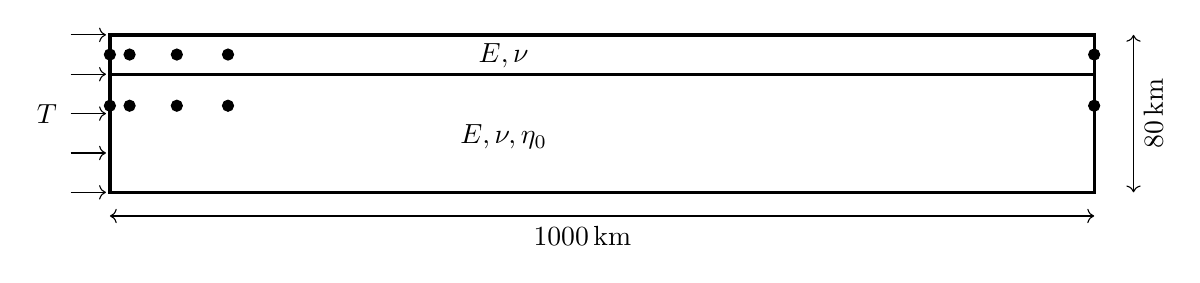
\begin{tikzpicture}
%\draw[step=0.5cm,gray,very thin] (0,0) grid (15,4); %background grid
\draw[very thick] (1,1)--(13.5,1)--(13.5,3)--(1,3)--cycle;  
\draw[very thick] (1,2.5)--(13.5,2.5);  
\draw[<->] (1,0.7)--(13.5,0.7);
\draw[<->] (14,1)--(14,3);
\node[] at (7,0.45) {$\SI{1000}{\km}$};
\node[rotate=90] at (14.25,2) {$\SI{80}{\km}$};
\node[] at (6,2.73) {$E,\nu$};
\node[] at (6,1.7) {$E,\nu,\eta_0$};
\draw[->] (0.5,3)--(0.95,3);
\draw[->] (0.5,2.5)--(0.95,2.5);
\draw[->] (0.5,2)--(0.95,2);
\draw[->] (0.5,1.5)--(0.95,1.5);
\draw[->] (0.5,1)--(0.95,1);
\node[] at (0.2,2) {$T$};

\filldraw[black] (1,2.75) circle (2pt);
\filldraw[black] (1,2.1) circle (2pt);

\filldraw[black] (1.25,2.75) circle (2pt);
\filldraw[black] (1.25,2.1) circle (2pt);

\filldraw[black] (1.85,2.75) circle (2pt);
\filldraw[black] (1.85,2.1) circle (2pt);

\filldraw[black] (2.5,2.75) circle (2pt);
\filldraw[black] (2.5,2.1) circle (2pt);

\filldraw[black] (13.5,2.75) circle (2pt);
\filldraw[black] (13.5,2.1) circle (2pt);
\end{tikzpicture}
\end{center}


After a thorough read of the paper, I have noticed quite a few problems:
\begin{itemize}
\item the paper is old and has been digitized but the figures are missing a lot of lines/shades/points ... this could be remedied by finding the article in a library.
\item in the intro it is stated: "Here we investigate the response of a lithosphere divided into upper elastic and lower uniform visco-elastic layers to simple boundary force and body force systems." The authors later talk about 'isostatic forces' opposing flexure. This means that buoyancy forces should be taken into account but there is no information about densities or gravity values!
\item little uncertainty about boundary conditions. is it free slip or no-slip on the right side ? Looking at fig 4, it looks like the vertical displacement is zero at x=1000km?
\item a Maxwell elasto-viscous rheology is used but this is only mentioned in the Appendix
\item the dimensions of the thinned or thickened areas is simply not mentioned. 
\item Fig~1 shows triangular elements. No mention is made of resolution, type of element, ndofs, resolution tests, any numerical detail whatsoever. Given the age of the paper, I would guess $P_1$
elements.
\item In the appendix they equate the viscous strain rate to $\sigma/4\eta$. Why 4 ?
\item it is also not clear whether the domain is ALE or fully Lagrangian: does it shorten?
\item the value of $T$ is never specified!
\item the paper was published 45 years ago, it is extremely unlikely any of the two authors is still available 
\end{itemize}

\begin{center}
\includegraphics[width=16cm]{images/viscoelasticity/kubo77}\\
{\captionfont Taken from \textcite{kubo77}. Measurement locations are indicated on 
the setup figure above. probably should be reversed}
\end{center}






%..........................................................
\subsubsection{Parallel-Plate Viscometer Problem - SNAC manual \label{v-e-snac}}

A parallel-plate viscometer problem is simulated, in which viscoelastic material is squeezed between two
parallel plates. The plates are moving at a constant velocity, $v_0$. Each plate has the length of $2L$ and 
is at a distance $2h$ from the other. No slip is assumed between the material and the plates. The approximate
analytical solution is given in the book by \textcite{jaeg69} (1969).

Model Setup: $L = 10~\si{\meter}$, $h=5~\si{\meter}$, viscosity $\eta=10^9~\si{\pascal\second}$, 
bulk modulus $K= 1.5~\si{\giga\pascal}$, shear modulus $\mu = 500~\si{\mega\pascal}$,
$v_0 = 10^{-4}~\si{\meter\per\second}$, $dt = 1~\si{\second}$ (results compared after 500 time steps),
mesh size: $20\times 10~\si{\meter}$, each element is a $1~\si{\meter}$ cube.

Due to the assumption of the original problem setup, artificial forces should be added to left and right
surfaces.

\begin{center}
\includegraphics[width=8cm]{images/viscoelasticity/snac_5}
\includegraphics[width=8cm]{images/viscoelasticity/snac_6}\\
{\captionfont 
Left: The initial mesh (blue) with the velocity boundary condition (red arrows);
Right: The second invariant of stress and velocities plotted on the deformed mesh. Colored arrows are
for SNAC’s solution, black ones for the analytic solution.}
\end{center}

$K=\lambda + \frac23 \mu$ so $\lambda=\frac{3500}{3}MPa$ ?

From wikipedia\footnote{\url{https://en.wikipedia.org/wiki/Lame_parameters}}
\[
\nu = \frac{3K-2\mu}{2(3K+\mu)} 
= \frac{4500-2*500}{2(4500+500)}
= \frac{3500}{10000}
= 0.35
\]
so we find that the material is {\color{orange} compressible $\nu=0.35$}

\[
E=\frac{9K\mu}{3K+\mu} 
=\frac{9*1500*500 MPa^2}{4500+500 MPa}
=\frac{9*1500*500}{5000} MPa
= 1350Mpa
\]


%..........................................................
\subsubsection{Relaxation after extention - Hassani syllabus}


{\color{orange} compressible $\nu=0.25$}

Un essai de relaxation consiste à imposer à un instant donné une déformation que 
l’on maintient constante par la suite. On observe alors comment évolue la contrainte au cours du temps.

The setup of the experiment is shown in the following figure:

\begin{center}
\includegraphics[width=9cm]{images/viscoelasticity/hassani_1}
\end{center}

The total duration of the experiment is $T=\SI{5}{\year}\simeq \SI{15.75e7}{\second}$.
The duration of the loading is $T/10=\SI{6}{months}$ while the duration 
of the subsequent relaxation is then $9T/10\simeq 4.5~\si{\year}$.

The loading velocity is $v=\SI{1}{\mm\per\year}\simeq \SI{3.17e-11}{\meter\per\second}$.
The sample has size $L\times L/2 = 20\times10\si{cm}$ and 
the strain rate is then $v/L \simeq \SI{1.5e-10}{\per\second}$.
Young's modulus is set to \SI{1e11}{\pascal} and the Poisson ratio is 0.25, i.e.
$\mu=40~\si{GPa}$. The viscosity is set to $\eta_0=\SI{1e18}{\pascal\second}$.
The Maxwell time is then $t_M=\eta/\mu=0.8~\si{\year}$, which is also the time it takes 
to reduce the maximum stress by a factor $e$.

\begin{center}
\includegraphics[width=6cm]{images/viscoelasticity/hassani_2}
\end{center}



 \label{chapt:viscoelasticity} %%%%%%%%%%%%%%%%%%%%%%%%%%%%%%%%%%%%%%%%%%%%%%%%%


%%%%%%%%%%%%%%%%%%%%%%%%%%%%%%%%%%%%%%%%%%%%%%%%%%%%%%%%%%%%%%%%%%%%%%%%%%%%%%%%%%%%%%%%%%%%%%%%%%%
%%%%%%%%%%%%%%%%%%%%%%%%%%%%%%%%%%%%%%%%%%%%%%%%%%%%%%%%%%%%%%%%%%%%%%%%%%%%%%%%%%%%%%%%%%%%%%%%%%%
\appendix %%%%%%%%%%%%%%%%%%%%%%%%%%%%%%%%%%%%%%%%%%%%%%%%%%%%%%%%%%%%%%%%%%%%%%%%%%%%%%%%%%%%%%%%%
%%%%%%%%%%%%%%%%%%%%%%%%%%%%%%%%%%%%%%%%%%%%%%%%%%%%%%%%%%%%%%%%%%%%%%%%%%%%%%%%%%%%%%%%%%%%%%%%%%%
%%%%%%%%%%%%%%%%%%%%%%%%%%%%%%%%%%%%%%%%%%%%%%%%%%%%%%%%%%%%%%%%%%%%%%%%%%%%%%%%%%%%%%%%%%%%%%%%%%%

\chapter{Codes in geodynamics \label{app:codes} }
In what follows I make a quick inventory of the main codes of computational geodynamics, 
for crust, lithosphere and/or mantle modelling.

in order to find all CIG-codes citations go to: https://geodynamics.org/cig/news/publications-refbase/

\begin{itemize}

%------------
\item ABAQUS

\cite{gedh02}
\cite{fumr03}
\cite{camg07}
\cite{kuhe09}
\cite{camg10}
\cite{makh09}
\cite{nalr12}
\cite{pevp15}


%------------
\item ADELI

\noindent
1997: \cite{hajc97}\\
2004: \cite{gocl04}\\
2006: \cite{vech06} \\
2008: \cite{boht08a}\cite{boht08b}\\
2012: \cite{gech12}\cite{gigh12}\\
2013: \cite{wahd13}\\
2015: \cite{ceag15}\\
2018: \cite{cegm18}\cite{gehn18}

%------------
\item ASPECT

This code is hosted by CIG at \url{https://geodynamics.org/cig/software/aspect/}. 
It is an open source community code based on the finite element library deal.II. 
It is massively parallel, relies on the p4est library for adaptive mesh refinement,
uses the Trilinos solver library, and can deal with 2D and 3D geometries. 

\cite{bahk07}
\cite{krhb12}
\cite{aupm15}
\cite{tosn15}
\cite{dahe16}
\cite{gadb16}
\cite{zhon16}
\cite{hepb17}
\cite{daef17}
\cite{hedg17}
\cite{robh17}
\cite{robu17}
\cite{aumh17}
\cite{thie17}
\cite{brsg17}
\cite{onmz17}
\cite{tasm17}
\cite{zhli17}
\cite{daga18}
\cite{onzh18}
\cite{gltf18}
\cite{heps18}
\cite{galh18}
\cite{peka18}
\cite{puth18}
\cite{brst18b}
\cite{baba19}
\cite{stbl19}
\cite{cocf19}
\cite{liki19}

%-------------
\item BASIL/ELLE \url{http://elle.ws/}
\cite{bokj08}
\cite{llor19}

%------------
\item CHIC 
\cite{norv15}

%------------
\item CitcomS and CITCOMCU

These codes are hosted by CIG at \url{https://geodynamics.org/cig/software/citcomcu/}
and \url{https://geodynamics.org/cig/software/citcoms/}.

\noindent
1996: \cite{somo96}\\
1997: \cite{mole97}\\
1998: \cite{moso98}\cite{zhgm98}\cite{vazh99}\\
2000: \cite{zhzm00}\cite{gumr00}\\
2001: \cite{bigu01}\\
2002: \cite{tagh02}\\
2003: \cite{vazh03}\cite{cogu03}\cite{bigu03}\\
2004: \cite{solo04}\\
2005: \cite{bihi05}\\
2006: \cite{beck06}\cite{pibf06}\cite{tact06}\cite{besb06}\cite{coli06}\\
2007: \cite{bihi07}\cite{zhzl07}\cite{magu07}\cite{bavi07}\cite{rimb07}\cite{mofm07}\cite{cobs07}\\
2008: \cite{dihf08}\cite{gamc08}\cite{zhmt08}\cite{hole08}\\
2009: \cite{lizh09}\cite{arhm09}\cite{zhzm09}\cite{anbi09}\cite{fobe09}\cite{bubi09}\cite{befa09}\cite{lezh09}\\
2010: \cite{bumb10}\cite{vabv10}\cite{baiv10}\cite{bubi10}\cite{zhzl10}\cite{bill10}\cite{jabi10}\\
2011: \cite{befa11}\cite{lemj11}\cite{vaal11}\cite{legu11}\cite{list11}\\
2012: \cite{arbi12}\cite{jabi12}\cite{bija12}\cite{bova12}\cite{hucf12}\cite{zhym12}\cite{solo12}
\cite{hibi12}\cite{jabk12}\cite{mapm12}\\
2013: \cite{bacs13}\cite{bogs13a}\cite{bogs13b}\cite{jabr13}\cite{qula13}\cite{oldh13}\cite{arbi13}\cite{cost13}\\
2014: \cite{flgw14}\cite{budt14}\cite{kava14}\cite{arfw14}\cite{wavp14}\cite{seki14}\cite{agvg14}
\cite{mabv14}\cite{zhu14}\\
2015: \cite{bacs15}\cite{bogf15}\cite{bomv15}\cite{sefw15}\cite{daso15}\cite{vami15}\cite{wazh15}
\cite{wavp15}\cite{waav15}\cite{hafg15}\cite{tarn15}\cite{legu15}\\
2016: \cite{welm16}\cite{wele16}\cite{jada16}\cite{frbs16}\\
2017: \cite{aggv17}\cite{maav17}\cite{frbm17}\cite{haja17}\\
2018: \cite{hect18}\cite{king18}\cite{kavb18}\\
2019: \cite{mavb19}\cite{fube19}\cite{magn19}\cite{malg19}\cite{mazh19}


\todo[inline]{cross check with CIG database}


%------------
\item CONMAN
This code is hosted by CIG at \url{https://geodynamics.org/cig/software/conman/}

\cite{kirh90}
\cite{itki94}
\cite{kian95}
\cite{kian98}
\cite{itki98}
\cite{befo99}
\cite{nake07}
\cite{dadh07}
\cite{kifr15}


%------------
\item CONVRS 
\cite{yoth12}
\cite{yosh13} 
 



%------------
\item DOUAR

\cite{brtf08}
\cite{thfb08}
\cite{yahb09}
\cite{brya10}
\cite{lobh10}
\cite{mutg13}
\cite{whbb14}
\cite{neew18}
\cite{koen19}

%------------
\item DYNEARTHSOL
\cite{chtl13}


\item ELMER
Elmer is an open source multiphysical simulation software mainly developed by 
CSC - IT Center for Science (CSC). Elmer development was started 1995 in collaboration with 
Finnish Universities, research institutes and industry. Elmer includes physical models of 
fluid dynamics, structural mechanics, electromagnetics, heat transfer and acoustics, 
for example. These are described by partial differential equations which Elmer solves 
by the Finite Element Method (FEM). \url{https://www.csc.fi/web/elmer}

\cite{mals14}


%------------
\item M-DOODS, Duretz code
\cite{yatd12}
\cite{yahb13}
\cite{chmd19}

%------------
\item FENICS
\cite{alrk14}


%------------
\item GAIA

\cite{hutm13}

%------------
\item GALE

This code is hosted by CIG at \url{https://geodynamics.org/cig/software/gale/}

\cite{fabs08}
\cite{gotc08}
\cite{beve10}
\cite{cmwt10}
\cite{lehm12}\cite{liqi12}
\cite{arbi13}

%------------
\item (G)TECTON

\noindent
1980: \cite{mera80}\\
1981: \cite{mera81}\\
1993: \cite{gowo93}\\
1995: \cite{gowo95}\\
1996: \cite{guez96}\\
1999: \cite{gowo99}\\
2001: \cite{bugw01}\cite{gome01}\\
2002: \cite{bugw02}\\
2005: \cite{gowo05}\cite{vanw05}\cite{vabl05}\\
2006: \cite{degw06}\cite{libi06}\cite{scdm06}\\
2007: \cite{vabl07}\\
2009: \cite{ladg09}\\
2011: \cite{bagw11}\cite{bagw11b}\\
2015: \cite{mags15}

%------------
\item ELEFANT

\cite{tosn15}
\cite{matv15}
\cite{busa16}
\cite{latb17}
\cite{thie17}
\cite{pltv18}
\cite{wohu19}

%-------------
\item ELLIPSIS

\cite{modm03}
\cite{omma06} 
\cite{moql07}
\cite{dyrm07}
\cite{onlg08}
\cite{pyeg10}
\cite{legu11}
\cite{lega12}


%------------
\item FANTOM
\index{FANTOM}

\cite{thie11}
\cite{alht11}
\cite{alht12}
\cite{alhf13}
\cite{erhv14}
\cite{thsh14}
\cite{erhv15}
\cite{erhv19}

%------------
\index FDCON

\cite{enbs05}
\cite{fusc13}
\cite{fuks15}


%------------
\index{FLUIDITY}
\item FLUIDITY
\cite{dawk11}
\cite{gagd14}

\index{geoFLAC}
\item geoFLAC (based on PARAVOZ)
\cite{jala19}

%------------
\index{IFISS}
\item IFISS: Incompressible Flow Iterative Solution Solver is a
MATLAB package that is a very useful tool for people interested in
learning about solving PDE’s.
IFISS includes built-in software for 2D versions of:
the Poisson equation, the convection-diffusion equation, the Stokes equations
and the Navier-Stokes equations.\\
\url{https://personalpages.manchester.ac.uk/staff/david.silvester/ifiss/}



%------------
\item the I2(3)E(L)VIS code

2003: \cite{geyu03}\cite{geyu03b}\cite{geur03}\\
2004: \cite{geym04}\cite{geys04}\cite{gepm04}\\
2005: \cite{buge05}\\
2006: \cite{bbeg06}\cite{gest06}\cite{gogc06}\cite{gecy06}\\
2007: \cite{geyu07}\cite{gogc07}\\
2008: \cite{scbe08}\cite{gecy08}\cite{uegs08}\cite{fagc08}\cite{zhgy09}\\
2009: \cite{gefc09}\\
2010: \cite{gerya2010}\cite{nigm10}\\
2011: \cite{dugm11}\cite{dumg11}\cite{lixg11}\cite{gery11}\cite{geme11}\\
2012: \cite{crsg12}\cite{dugk12}\cite{lixg12}\cite{fagm12}\\
2013: \cite{lixg13}\cite{nabg13}\cite{magc13}\cite{vagd13a}\cite{vagd13b}\cite{zhgt13}\cite{dyge13}\cite{gemd13}\cite{mana13}\\
2014: \cite{dugs14}\cite{puge14}\cite{rugb14}\cite{voge14b}\cite{bagb14}\cite{lige14}\cite{stjm14}\cite{malg14}
\cite{buge14}\cite{gosk14}\cite{bagb14}\cite{vamd14}\\
2015: \cite{duay15}\cite{uewg15}\cite{rula15}\cite{gesb15}\cite{rula15}\\
2016: \cite{kobc16}\cite{magc16}\cite{fige16}\\
2019: \cite{kobg19}\cite{ligc19}

%------------
\item I3MG
\cite{facc14}

%------------
\item LAMEM
\cite{scbe08}
\cite{kamm10}
\cite{lemk11}
\cite{may12}
\cite{lesh14}
\cite{cokm14}
\cite{bakp14}
\cite{feka14a}
\cite{feka14b}
\cite{puka15}
\cite{feka15}
\cite{cofk15}
\cite{kapb16}

%------------
\item LAPEX2D (LAgrangian Particle EXplicit, based on the prototype code PAROVOZ) 
\cite{sopg05}
\cite{bbeg06}\cite{basv06}
\cite{baso08}
\cite{scbe08}
\cite{sosk11}


%-------------
\item LITMOD
\cite{afrf07}
\cite{affr08}
\cite{fuac09}
\cite{fufa10}


%------------
\item MARC
\cite{nesg97}
\cite{nesb99}


%------------
\item MILAMIN

MILAMIN is a finite element method implementation in native MATLAB that is capable of doing one million degrees of freedom per minute on a modern desktop computer. This includes pre-processing, solving, and post-processing. The MILAMIN strategies and package are applicable to a broad class of problems in Earth science. \url{http://milamin.org/}

\noindent
2008: \cite{daks08}\\
2010: \cite{krda10}\cite{kaus10}\\
2011: \cite{yakm11}\\
2012: \cite{gebk12}\\
2014: \cite{jobk14}\\
2015: \cite{lukz15}\cite{gehm15}\cite{thkp15}\cite{musd15}\\
2016: \cite{jads16}\cite{maka16}\\
2018: \cite{dusd18}\cite{jasc18}\cite{jadg18}\cite{comj18}\cite{jens18}\cite{rabw18}\cite{chsm18}\\
2019: \cite{anpa19}\cite{sifg19}\cite{baba19}


%------------
\item PARAVOZ/FLAMAR/FLAC

\noindent
1989: \cite{cund89}\\
1993: \cite{poli93}\\
1996: \cite{hach96}\\
1998: \cite{gepd98}\\
2000: \cite{labp00}\\
2001: \cite{bujl01}\cite{bupo01}\\
2002: \cite{bast02}\cite{clbb02}\\
2003: \cite{hags03}\cite{gehd03}\cite{upke03}\\
2004: \cite{guhl04}\cite{gewi04}\cite{toba04}\cite{tibb04}\\
2005: \cite{bugu05}\\
2007: \cite{yaab07}\cite{buto07}\\
2008: \cite{yaba08}\cite{tibb08}\\
2009: \cite{gecm09}\cite{yahb09}\cite{bucl09}\\
2012: \cite{anwb12}\cite{gech12}\cite{gubc12}\cite{gerb12}\\
2013: \cite{wabd13}\cite{frbm13}\\
2014: \cite{frba14}\cite{gagb14}\cite{bufa14}\\
2015: \cite{wulc15}\cite{marl15}\cite{gebw15}\cite{svlh15}\\




%------------
\item PINK3D
\cite{vosc15}


%------------
\item PLASTI
\cite{fuwb06}



%------------
\item pTatin3D: A nice succinct description of the code is given in Appendix B of \cite{lemh17}.

2013: \cite{phil13}\\
2014: \cite{mabl14}\\
2015: \cite{mabl15}\\
2017: \cite{lemh17}\\
2018: \cite{jolp18}\\
2019: \cite{jolm19}

%---------------------
\item Pylith

\cite{aakw13}


%------------
\item RHEA
\cite{bugg08}
\cite{stgb10}
\cite{algs12}
\cite{busa13}

%------------
\item SAMOVAR
\cite{egat10}

%------------
\item SEPRAN

1993: \cite{beky93}\cite{vavy93}\\
1994: \cite{vlvv94}\cite{vayv94}\\
1995: \cite{vayv95}\\
1996: \cite{vayu96}\\
2002: \cite{civv02}\cite{vavv02}\\
2003: \cite{vavs03}\\
2004: \cite{vavv04}\cite{vavv04b}\cite{vavv04c}\\
2005: \cite{vavv05}\cite{sepr05}\\
2006: \cite{liva06a}\cite{liva06b}\\
2007: \cite{vant07}\cite{civv07}\cite{brva07a}\cite{brva07b}\\
2008: \cite{plva08}\\
2009: \cite{vavl09}\\
2010: \cite{vahy10}\cite{syva10}\\
2011: \cite{vahs11}\\
2012: \cite{besy12}\cite{beva12}\cite{chgv12}\\
2013: \cite{ancv13}\\
2014: \cite{chsg14}\cite{mova14}\\
2015: \cite{vasy15}\\
2019: \cite{zhdv19}\cite{vayu19}

%------------
\item SISTER

\cite{olbm16}

%------------
\item SLIM3D

\cite{poso08}
\cite{qusp10}
\cite{brps12}
\cite{brps13}
\cite{brau13}
\cite{brun14}
\cite{hebr14}
\cite{kobf14}
\cite{clbq15}
\cite{brcr17}
\cite{basq18}

%------------
\item SLOMO
\cite{kaus05}

%------------
\index SNAC
\cite{chlg08}


%------------
\item SOPALE

1994: \cite{wibe94}\cite{befh94}\\
1995: \cite{full95}\cite{elfb95}\\
1996: \cite{bekh96}\\
1999: \cite{will99a}\cite{will99b}\\
2000: \cite{pybf00}\cite{bemh00}\\
2001: \cite{bejn01}\\
2002: \cite{hube02}\cite{pybf02}\\
2003: \cite{hube03}\cite{vamf03}\cite{wipo03}\cite{pymi03}\\
2004: \cite{bejn04}\cite{pycr04}\cite{pybe04}\cite{elsp04}\cite{geim04}\\
2005: \cite{gebi05}\cite{hubb05}\\
2006: \cite{pysk06}\cite{selz06}\\
2007: \cite{hube07}\cite{cubh07}\cite{mohb07}\\
2008: \cite{sebp08}\cite{wabj08}\cite{wabj08b}\cite{gopy08}\\
2009: \cite{kecw09}\cite{bejb09}\cite{bupb09}\cite{grba09}\cite{sihb09}\\
2010: \cite{albs10}\cite{albe10}\cite{grpy10}\cite{pygp10}\\
2011: \cite{cube11}\cite{bubj11}\cite{hube11}\\
2012: \cite{grpy12}\cite{grpy12b}\cite{kogp12}\cite{grbe12}\cite{jahu12}\\
2013: \cite{bubj13}\cite{chbe13}\cite{fihv13a}\cite{fihv13b}\cite{gobi13}\cite{grpy13}\cite{knak13}\cite{nipc13}\cite{jahm13}\\
2014: \cite{gogu14}\\
2015: \cite{albe15}\cite{bubj15}\cite{heps15}\\
2016: \cite{licu16}\\
2017: \cite{bube17}


%------------
\item STAGYY
\cite{rota11}
\cite{yadl14}
\cite{crta14}
\cite{cosh18}
\cite{gult19}

%------------
\item SUBMAR

\cite{masr06}
\cite{masp07}
\cite{roms10}


%------------
\item SULEC
SULEC is a finite element code that solves the incompressible Navier-Stokes equations 
for slow creeping flows. The code is developed by Susan Ellis 
(GNS Sciences, NZ) and Susanne Buiter (NGU). 
\url{http://www.geodynamics.no/buiter/sulec.html}

\noindent
2011: \cite{qube11}\cite{ellw11}\\
2012: \cite{buit12}\cite{tebu12}\cite{crsg12}\cite{grel12}\\
2013: \cite{ghbu13}\\
2014: \cite{ghbu14}\cite{qubu14}\\
2015: \cite{nabu15}\\
2016: \cite{zwsn16}\\
2017: \cite{nabp17}\\
2018: \cite{tebu18}











%------------
\item TERRA:
The computational grid is based on a projection of the regular icosahedron onto a 
sphere and successive dyadic refinements \cite{bafr85}.  Concentric copies of such  
spherical layers of nodes build the domain in radial direction.

\cite{baum83}
\cite{glat88}
\cite{buba95}
\cite{burb97}\cite{yang97}
\cite{burl98}
\cite{phbs09}\cite{wodd09}\cite{gows09}
\cite{woda11}
\cite{dadb13}
\cite{vade16}

\index{TerraFERMA}
\item TerraFERMA
\cite{wisv14}
\cite{wisv17}
\cite{spmw16}
\cite{ceww17}
\cite{ceww19}


%------------
\item YACC
\cite{tosn15}
\cite{tomy16}

%------------
\item UNDERWORLD 1\&2

\noindent
2006: \cite{stfs06}\\
2007: \cite{moql07}\cite{stfs07}\\
2008: \cite{lemm08}\cite{ozrs08}\cite{gotc08}\\
2010: \cite{casm10}\cite{mamb10}\cite{stsf10}\cite{stfc10}\cite{fasm10}\\
2011: \cite{memm11}\cite{cafz11}\\
2012: \cite{cafa12}\\
2013: \cite{bemm13}\cite{scmo13}\cite{faca13}\cite{care13}\\
2014: \cite{famc14}\\
2015: \cite{quxm15}\cite{bemm15}\cite{scsp15}\cite{shmj15}\\
2016: \cite{shmv16}\cite{onlw16}\cite{kicf16}\\
2018: \cite{memm18}\\
2019: \cite{samo19}\cite{yamg19}

\item VEMAN
\cite{bepo10}


\end{itemize}
 %%%%%%%%%%%%%%%%%%%%%%%%%%%%%%%%%%%%
\chapter{Matrix properties} \subsection{Symmetric matrices}

Any {\sl symmetric} matrix 
has only real eigenvalues,
is always diagonalizable,
and has orthogonal eigenvectors.
A symmetric $N\times N$ real matrix ${\bm M}$ is said to be
\begin{itemize}
\item {\bf positive definite} if $\vec x \cdot {\bm M} \cdot \vec x >0$ for every non-zero vector $\vec x$ of n real numbers. All the eigenvalues of a  Symmetric Positive Definite (SPD) matrix are positive.
 If A and B are positive definite, then so is A+B.
The matrix inverse of a positive definite matrix is also positive definite.
An SPD matrix has a unique Cholesky decomposition. In other words the matrix ${\bm M}$ 
is positive definite if and only if there exists a unique
lower triangular matrix ${\bm L}$, with real and strictly positive diagonal elements, 
such that ${\bm M} = {\bm L}{\bm L}^T$
(the product of a lower triangular matrix and its conjugate transpose).
This factorization is called the Cholesky decomposition of ${\bm M}$.
\index{general}{Symmetric Positive Definite}

\item {\bf positive semi-definite} if $\vec x \cdot {\bm M} \cdot  \vec x \geq 0$
\item {\bf negative definite} if $\vec x \cdot {\bm M} \cdot \vec x < 0$
\item {\bf negative semi-definite} if $\vec x \cdot {\bm M} \cdot \vec x \leq 0$
\end{itemize}

The Stokes linear system
\[
\left( \begin{array}{cc}
\mathbb{K} & \mathbb{G}  \\ \mathbb{G}^T &  0
\end{array} \right) \cdot
\left( \begin{array}{c}  {\bm v} \\ {\bm p}  \end{array} \right) = 
\left( \begin{array}{c}  {\bm f} \\ {\bm g}  \end{array} \right) 
\]
is {\bf indefinite} (i.e. it has positive as well as negative eigenvalues).

A square matrix that is not invertible is called {\bf singular} or degenerate. A square matrix is singular if and only if its determinant is 0. Singular matrices are rare in the sense that if you pick a random square matrix, it will almost surely not be singular.

%--------------------------------
\subsection{Schur complement}

From wiki.
In linear algebra and the theory of matrices, the Schur complement of a matrix block (i.e., a submatrix within a larger matrix) is defined as follows.
Suppose ${\bm A}$, ${\bm B}$, ${\bm C}$, ${\bm D}$
are respectively $p\times p$, $p \times q$, $q \times p$ and $q \times q$ matrices, and $\mathbb{D}$ is invertible. Let
\[
{\bm M}=
\left( \begin{array}{cc}
{\bm A} & {\bm B}  \\ 
{\bm C} & {\bm D}
\end{array} \right) 
\]
so that ${\bm M}$ is a $(p+q)\times(p+q)$ matrix.
Then the Schur complement of the block ${\bm D}$ of the matrix ${\bm M}$ is the $p \times p$ matrix
\[
{\bm S}={\bm A}-{\bm B}\cdot {\bm D}^{-1}\cdot {\bm C}
\]
Application to solving linear equations: The Schur complement arises naturally 
in solving a system of linear equations such as
\begin{eqnarray}
{\bm A}\cdot\vec x+{\bm B}\cdot \vec y &=& \vec f \nonumber\\
{\bm C}\cdot\vec x+{\bm D}\cdot \vec y &=& \vec g \nonumber
\end{eqnarray}
where $\vec x$, $\vec f$ are $p$-dimensional vectors, $\vec y$, $\vec g$
are $q$-dimensional vectors,
and ${\bm A}$, ${\bm B}$, ${\bm C}$, ${\bm D}$ are as above.
Multiplying the bottom equation by ${\bm B}\cdot {\bm D}^{-1}$ 
and then subtracting from the top equation one obtains
\[
({\bm A}-{\bm B}\cdot {\bm D}^{-1}\cdot {\bm C})\cdot \vec x = \vec f - {\bm B}\cdot {\bm D}^{-1}\cdot \vec g
\]
Thus if one can invert ${\bm D}$ as well as the Schur complement of ${\bm D}$, one can solve for $\vec x$,
and then by using the equation $\bm C\cdot \vec x + \bm D \cdot \vec y = \vec g$ one can solve for $y$.
This reduces the problem of inverting a $(p+q) \times (p+q)$ matrix to that of inverting
a $p \times p$ matrix and a $q \times q$ matrix.
In practice one needs ${\bm D}$ to be well-conditioned in order for 
this algorithm to be numerically accurate.

Considering now the Stokes system: 
\[
\left( \begin{array}{cc}
\K & \G  \\ \G^T &  -\C
\end{array} \right) \cdot
\left( \begin{array}{c}  {\vec v} \\ {\vec p}  \end{array} \right) = 
\left( \begin{array}{c}  {\vec f} \\ {\vec g}  \end{array} \right) 
\]
Factorising for ${\vec p}$ we end up with a {\bf velocity-Schur complement}.
Solving for ${\vec p}$ in the second equation and inserting the expression
for ${\vec p}$ into the first equation we have
\[
\mathbb{S}_v \cdot {\vec v}  = {\vec f} 
\quad\quad
\text{with}
\quad\quad
\mathbb{S}_v=\K+ \G \cdot \C^{-1} \cdot \G^T
\]
Factorising for $\vec v$ we get a {\bf pressure-Schur complement}.
\[
\mathbb{S}_p \cdot {\vec p}  = \G^T \cdot \K^{-1}\cdot {\vec f}
\quad\quad
\text{with}
\quad\quad
\mathbb{S}_p = \G^T \cdot \K^{-1}\cdot \G + \C 
\]


 %%%%%%%%%%%%%%%%%%%%%%%%%%%%%%%%%%%%%%%%%%%%%%%%%%%%%%
\chapter{Don't be a hero - unless you have to} What follows was published online on July 17th, 2017 at 
\url{https://blogs.egu.eu/divisions/gd/2017/07/19/dont-be-a-hero-unless-you-have-to/}
It was written by me and edited by Iris van Zelst, at the time PhD student at ETH Z\"urich.

\vspace{3mm}

In December 2013, I was invited to give a talk about the \aspect{} code [1] 
at the American Geological Union conference in San Francisco. Right 
after my talk, Prof. Louis Moresi took the stage and gave a talk entitled: 
{\it Underworld: What we set out to do, How far did we get, What did we Learn?}

The abstract went as follows:

"Underworld was conceived as a tool for modelling 3D lithospheric deformation coupled with the underlying / surrounding mantle flow. The challenges involved were to find a method capable of representing the complicated, non-linear, history dependent rheology of the near surface as well as being able to model mantle convection, and, simultaneously, to be able to solve the numerical system efficiently. […] The elegance of the method is that it can be completely described in a couple of sentences. However, there are some limitations: it is not obvious how to retain this elegance for unstructured or adaptive meshes, arbitrary element types are not sufficiently well integrated by the simple quadrature approach, and swarms of particles representing volumes are usually an inefficient representation of surfaces."

Aside from the standard numerical modelling jargon, Louis used a term during his talk which I thought at the time had a nice ring to it: hero codes. In short, I believe he meant the codes written essentially by one or two people who at some point in time spent great effort into writing a code (usually choosing a range of applications, a geometry, a number of dimensions, a particular numerical method to solve the relevant PDEs(1), and a tracking method for the various fields of interest).

In the long list of Hero codes, one could cite (in alphabetical order) CITCOM [1], \douar [8], \fantom [2], IELVIS [5], LaMEM [3], pTatin [4], SLIM3D [10], \sopale [7], StaggYY [6], \sulec [11], Underworld [9], and I apologise to all other heroes out there whom I may have overlooked. And who does not want to be a hero? The Spiderman of geodynamics, the Superwoman of modelling?

Louis' talk echoed my thoughts on two key choices we (computational geodynamicists) are facing: Hero or not, and if yes, what type?

\vspace{3mm}

{\bf Hero or not?}

\vspace{3mm}

Speaking from experience, it is an intense source of satisfaction when peer-reviewed published results are obtained with the very code one has painstakingly put together over months, if not years. But is it worth it?

On the one hand, writing one own’s code is a source of deep learning, a way to ensure that one understands the tool and knows its limitations, and a way to ensure that the code has the appropriate combination of features which are necessary to answer the research question at hand. On the other hand, it is akin to a journey; a rather long term commitment; a sometimes frustrating endeavour, with no guarantee of success. Let us not deny it – many a student has started with one code only to switch to plan B sooner or later. Ultimately, this yiels a satisfactory tool with often little to no perennial survival over the 5 year mark, a scarce if at all existent documentation, and almost always not compliant with the growing trend of long term repeatability. Furthermore, the resulting code will probably bear the marks of its not-all-knowing creator in its DNA and is likely not to be optimal nor efficient by modern computational standards.

This brings me to the second choice: elegance \& modularity or taylored code \& raw performance? Should one develop a code in a very broad framework using as much external libraries as possible or is there still space for true heroism?

It is my opinion that the answer to this question is: both. The current form of heroism no more lies in writing one’s own FEM(2)/FDM(3) packages, meshers, or solvers from scratch, but in cleverly taking advantage of state-of-the-art packages such as for example p4est [15] for Adaptive Mesh Refinement, PetSc [13] or Trilinos [14] for solvers, Saint Germain [17] for particle tracking, deal.ii [12] or Fenics [16] for FEM, and sharing their codes through platforms such as svn, bitbucket or github.

In reality, the many different ways of approaching the development or usage of a (new) code is linked to the diversity of individual projects, but ultimately anyone who dares to touch a code (let alone write one) is a hero in his/her own right: although (super-)heroes can be awesome on their own, they often complete each other, team up and join forces for maximum efficiency. Let us all be heroes, then, and join efforts to serve Science to the best of our abilities.

\vspace{3mm}

\noindent Abbreviations

(1) PDE: Partial Differential Equation 

(2) FEM: Finite Element Method 

(3) FDM: Finite Difference Method

\noindent References

[1] Zhong et al., JGR 105, 2000; 

[2] Thieulot, PEPI 188, 2011; 

[3] Kaus et al., NIC Symposium proceedings, 2016; 

[4] May et al, CMAME 290, 2015 

[5] Gerya and Yuen, PEPI 163, 2007 

[6] Tackley, PEPI 171, 2008 

[7] Fullsack, GJI 120, 1995 

[8] Braun et al., PEPI 171, 2008 

[9] http://www.underworldcode.org/ 

[10] Popov and Sobolev, PEPI 171, 2008 

[11] http://www.geodynamics.no/buiter/sulec.html 

[12] Bangerth et al., J. Numer. Math., 2016; http://www.dealii.org/ 

[13] http://www.mcs.anl.gov/petsc/ 

[14] https://trilinos.org/ 

[15] Burstedde et al., SIAM journal on Scientific Computing, 2011; http://www.p4est.org/ 

[16] https://fenicsproject.org/ 

[17] Quenette et al., Proceedings 19th IEEE, 2007





 %%%%%%%%%%%%%%%%%%%%%%%%%%%%%%%%%%%%%%%
\chapter{A \fantom, an \elefant and a \ghost} While a post-doctoral researcher at Bergen University I developed the FANTOM code. Here is what other people and I have published with it:

\begin{itemize}

\item {\it FANTOM : two- and three-dimensional numerical modelling of creeping flows for the solution of geological problems}, 
C. Thieulot, Physics of the Earth and Planetary Interiors, 188, 2011.

\begin{center}
\includegraphics[width=8cm]{images/mycodes/thie11_img}
\end{center}


\item {\it Three-dimensional numerical modeling of upper crustal extensional systems}, 
V. Allken, R.S. Huismans and C. Thieulot, JGR 116, 2011. \url{https://doi:10.1029/2011JB008319} 

\begin{center}
\includegraphics[height=3cm]{images/mycodes/alht11_img}
\end{center}


\item {\it Factors controlling the mode of rift interaction in brittle-ductile coupled systems: A 3D numerical study}, 
V. Allken, R.S. Huismans and C. Thieulot, Geochem. Geophys. Geosyst. 13(5), 2012.
\url{https://doi:10.1029/2012GC004077}

\begin{center}
\includegraphics[height=3cm]{images/mycodes/alht12_img}
\end{center}


\item {\it 3D numerical modelling of graben interaction and linkage: a case study of the Canyonlands grabens, Utah}, 
V. Allken, R.S. Huismans, Haakon Fossen and C. Thieulot, Basin Research, 25, 1-14, 2013.
\url{https://doi: 10.1111/bre.12010}

\begin{center}
\includegraphics[height=3cm]{images/mycodes/alhf13_img}
\end{center}


\item {\it Three-dimensional numerical simulations of crustal systems undergoing orogeny and subjected to surface processes}, 
C. Thieulot, P. Steer and R.S. Huismans, Geochem. Geophys. Geosyst., 15, 2014. doi:10.1002/2014GC005490

\item {\it Extensional inheritance and surface processes as controlling factors of mountain belt structure}, 
Z. Erd\"os, R.S. Huismans, P. van der Beek, and C. Thieulot, J. Geophys. Res. Solid Earth, 119, 2014. doi:10.1002/2014JB011408

\item {\it First-order control of syntectonic sedimentation on crustal-scale structure of mountain belts}, 
Z. Erd\"os, R.S. Huismans, P. van der Beek, J. Geophys. Res. Solid Earth, 120, 5362-5377, 2015. doi:10.1002/2014JB011785

\item {\it The Wilson Cycle and Effects of Tectonic Structural Inheritance
on Rifted Passive Margin Formation}, C.A. Salazar-Mora, R.S. Huismans, H. Fossen and M. Egydio-Silva, 
Tectonics, 37, 3085-3101, 2017. 01. doi:10.1029/2018TC004962 

\begin{center}
\includegraphics[height=5cm]{images/mycodes/sahf18_img}
\end{center}


\item {\it Control of increased sedimentation on orogenic fold-and-thrust belt structure - 
insights into the evolution of the Western Alps}, 
Z. Erd\"os, R.S. Huismans and P. van der Beek, Solid Earth, 10, 391-404, 2019.
\url{https://doi.org/10.5194/se-10-391-2019}

\begin{center}
\includegraphics[height=3cm]{images/mycodes/erhv19_img}
\end{center}

\item {\it Mountain building or backarc extension in ocean-continent subduction systems - a function of
backarc lithospheric strength and absolute plate velocities}, 
S.G. Wolf and R.S. Huismans, JGR, 2019. \url{https://doi.org/10.1029/2018JB017171}

\begin{center}
\includegraphics[height=3cm]{images/mycodes/wohu19_img}
\end{center}


\end{itemize}

Upon my arrival at Utrecht University in 2012 I started working an a more flexible code, called ELEFANT, which has since very much 
diverged from FANTOM.

\begin{itemize}
\item {\it The effect of obliquity on temperature in subduction zones: insights from 3-D numerical modeling}, 
A. Plunder, C. Thieulot and D.J.J. van Hinsbergen, Solid Earth 9, 759-776, 2018. \url{https://doi.org/10.5194/se-9-759-2018}

\begin{center}
\includegraphics[height=3.5cm]{images/mycodes/pltv18_img}
\end{center}


\item {\it Analytical solution for viscous incompressible Stokes flow in a spherical shell}, 
C. Thieulot, Solid Earth 8, 1181-1191, 2017. \url{https://doi.org/10.5194/se-8-1181-2017}

\begin{center}
\includegraphics[height=3cm]{images/mycodes/thie17}
\end{center}



\item  {\it Lithosphere erosion and continental breakup: interaction of extension, plume upwelling and melting}, 
A. Lavecchia, C. Thieulot, F. Beekman, S. Cloetingh and S. Clark, E.P.S.L. 467, p89-98, 2017.

\begin{center}
\includegraphics[height=3cm]{images/mycodes/latv17_img}
\end{center}


\item {\it Benchmarking numerical models of brittle thrust wedges}, 
Susanne J.H. Buiter, Guido Schreurs, Markus Albertz, Taras V. Gerya, Boris Kaus,
Walter Landry, Laetitia le Pourhiet, Yury Mishin, David L. Egholm, Michele Cooke,
Bertrand Maillot, Cedric Thieulot, Tony Crook, Dave May, Pauline Souloumiac, Christopher Beaumont
Journal of Structural Geology 92, p140-177, 2016. \url{https://doi:10.1016/j.jsg.2016.03.003}

\begin{center}
\includegraphics[height=1.8cm]{images/mycodes/busa16_img}
\end{center}


\item {\it A community benchmark for viscoplastic thermal convection in a 2-D square box}, 
N. Tosi, C. Stein, L. Noack, C. Huettig, P. Maierova, H. Samuel, D.R. Davies, C.R. Wilson, S.C. Kramer, C. Thieulot, A. Glerum, M. Fraters, W. Spakman, A. Rozel, P.J. Tackley, Geochem. Geophys. Geosyst. 16, doi:10.1002/2015GC005807, 2015.

\begin{center}
\includegraphics[height=3cm]{images/mycodes/tosn15_img}
\end{center}


\item {\it Dynamics of intraoceanic subduction initiation: 1. Oceanic detachment fault inversion and the formation of supra-subduction zone ophiolites}, M. Maffione, C. Thieulot, D.J.J. van Hinsbergen, A. Morris, O. Pluemper and W. Spakman, Geochem. Geophys. Geosyst. 16, p1753-1770, 2015.

\begin{center}
\includegraphics[height=1.8cm]{images/mycodes/matv15_img}
\end{center}

\item {\it The Geodynamic World Builder: a solution for complex initial conditions in numerical modelling},
M. Fraters, C. Thieulot, A. van den Berg and W. Spakman,
Solid Earth, \url{https://doi.org/10.5194/se-2019-24}, 2019.

\begin{center}
\includegraphics[height=2.8cm]{images/mycodes/frtv19_img}
\end{center}


\end{itemize}


\begin{itemize}
\item {\it GHOST: Geoscientific Hollow Sphere Tessellation}, 
C. Thieulot, Solid Earth, 9, 1169–1177, 2018. \url{https://doi.org/10.5194/se-9-1169-2018}

\begin{center}
\includegraphics[height=3cm]{images/mycodes/shell_HS06}
\includegraphics[height=3cm]{images/mycodes/shell_HS12}
\includegraphics[height=3cm]{images/mycodes/shell_HS20}
\end{center}

\end{itemize}

 %%%%%%%%%%%%%%%%%%%%%%%%%%%%%%%%%%%%%
\chapter{Some useful Python commands} \begin{flushright} {\tiny {\color{gray} app\_useful\_python.tex}} \end{flushright}

%--------------------------
\subsection{Sparse matrices}

So far, the best way I have found to deal with sparse matrices is to 
declare the matrix as a 'lil\_matrix' (linked list).

\begin{lstlisting}
from scipy.sparse import csr_matrix, lil_matrix
A_mat = lil_matrix((Nfem,Nfem),dtype=np.float64)
\end{lstlisting}

One then adds terms to it as if it was a full/dense matrix. 
Once the assembly is done, the conversion to CSR format is trivial:

\begin{lstlisting}
A_mat=A_mat.tocsr()
\end{lstlisting}

Finally the solver can be called:

\begin{lstlisting}
sol=sps.linalg.spsolve(A_mat,rhs)
\end{lstlisting}

%--------------------------
\subsection{condition number}

if the matrix has been declared as lil\_matrix, first convert it to a dense matrix:
\begin{lstlisting}
A_mat=A_mat.dense()
\end{lstlisting}
The condition number of the matrix is simply obtained as follows:
\begin{lstlisting}
from numpy import linalg as LA
print(LA.cond(A_mat))
\end{lstlisting}

%--------------------------
\subsection{Weird stuff}

Python is touted as the one language students should learn and master. However it is a language which allows *way* too much liberty in its syntax and encourages students to be sloppy. 

For instance the following code runs just fine:

\begin{lstlisting}
for k in range(0,5): 
    for k in range(0,5):
        for k in range(0,5):
            print (k)
\end{lstlisting}

This alone should disqualify this language. It is easy to see the obvious problem with this code, but adding a few lines of code in between each 'for' line hides the problem and the absence of any warning makes this code a nightmare to debug.



\begin{verbatim}
https://www.w3schools.com/python/default.asp

https://www.codecademy.com/learn/learn-python

https://learnpythonthehardway.org/book/
\end{verbatim}

%----------------------------------
\subsection{Making simple 2D plots}

\begin{lstlisting}
import matplotlib.pyplot as plt

# number of points
N=100

# a despicable way of filling two arrays
x_data=[]
y_data=[]
for i in range(0,N):
    x=i
    y=i**2+2*i+1.
    x_data.append(x)
    y_data.append(y)

# generating a 2D figure with the data
plt.figure()
plt.plot(x_data,y_data, label = 'name of data')
plt.xlabel('x-axis label')
plt.ylabel('y-axis label')
plt.legend()
plt.savefig('myplot.pdf', bbox_inches='tight')
plt.show()
\end{lstlisting}

\begin{center}
\includegraphics[width=7cm]{images/python/myplot}
\end{center}



%----------------------------------
\subsection{Making simple 3D plots of scatter}

\begin{lstlisting}
fig = plt.figure()
ax = plt.axes(projection='3d')
ax.set_title("insert here text for title")
size = ..some value..
ax.scatter3D(x, y, z, s = size)
\end{lstlisting}




%----------------------------------
\subsection{How to debug your code}


Debugging a FE code is by no means trivial. There is (at least) a grid, a connectivity array, basis functions and their derivatives, the elemental matrices and rhs, the assembly, boundary conditions, and a call to a solver before the solution (if the solver returns one!) can be visualised. 
\begin{itemize}
\item First and foremost, make sure that your grid of points is correct.
For instance, you can resort to exporting it to an ascii file as follows:
\begin{lstlisting}
np.savetxt('velocity.ascii',np.array([x,y,u,v]).T,header='# x,y,u,v')
\end{lstlisting}
In two dimensions, you should set for example nelx=3 and nely=2, so that 
for $Q_1$ elements the grid counts 12 points. Then make sure the coordinates and the order of the points makes sense. 
Repeat the process for pressure nodes, temperature nodes, etc ...

\item Then it is time to check the connectivity array(s). 
\begin{lstlisting}
for iel in range (0,nel):
   print ("iel=",iel)
   for k in range(0,m)
      print ("node ",icon[0,iel],"at pos.",x[icon[0,iel]], y[icon[0,iel]])
\end{lstlisting}
This displays the list of nodes and their positions making each element.
Repeat the process for every connectivity array.

\item We can go on with testing that the all basis functions are 1 on their node and  zero elsewhere:
\begin{lstlisting}
for i in range(0,m):
   print ('node',i,':',NNV(rnodes[i],snodes[i]))
\end{lstlisting}
here the arrays rnodes and snodes contain the (r,s) coordinates of the m nodes 

\item test jacobian, compute volume of domain

\item sum(dNNNdx)=0

\item print nodes where bc 

\end{itemize}

%----------------------------------
\subsection{Optional arguments}

Courtesy of Henry Brett.

\begin{lstlisting}
def myfunc(a,b, *optional_arguments, **keyword_arguments):
    print(a)
    print(b)
    for ar in optional_arguments:
        print(ar)
    d=keyword_arguments.get("d", None)
    print(d)
    

a="dog"
b="cat"
myfunc(a,b,"shrek","fiona",d="donkey")
\end{lstlisting}

%----------------------------------
\subsection{drawing and filling quadrilaterals}

\begin{lstlisting}
import matplotlib.pyplot as plt

plt.figure(figsize=(3, 3))
plt.axis('equal')

x=(1,1.5,1.6,0.8)
y=(0,-0.1,1.5,1.2)
plt.fill(x, y,"b")

x=(0,0.5,0.6,-0.2)
y=(0,-0.4,1.1,1.1)
plt.fill(x, y,"r")

plt.savefig('xxx.pdf')
plt.show()

\end{lstlisting}

\begin{center}
\includegraphics[width=5cm]{images/python/xxx}
\end{center}






 %%%%%%%%%%%%%%%%%%%%%%%%%%%%%%%%%%%
\chapter{Some useful maths} \input{app_maths} \label{app_maths} %%%%%%%%%%%%%%%%%%%%%%%%%%%%%%%%%%%
\chapter{Elemental matrices for simple geometries}\label{app:mm} \begin{flushright} {\tiny {\color{gray} app\_elemental\_matrix.tex}} \end{flushright}

In what follows I compute the mass matrix for a variety of reference elements.
If you wish to use these in a code, do not forget to take the jacobian 
of the transformation/mapping into account. 

%---------------------------
\section{1d segments}

%.....................................
\subsection{Linear basis functions}

Let us start with the mass matrix (which we encountered in 
Section~\ref{sec:diff1D} -- although we leave the $\rho C_p$ term out, 
thereby implicitely assuming it is constant over the element!):
\begin{equation}
{\bm M}_e=\int_{\Omega_e} \vec{\bN}^T \vec{\bN} dV
= \int_{-1}^{+1} \vec{\bN}^T \vec{\bN} dr
\end{equation}
on the reference element, with 
\[
{\vec N}^T = 
\left(
\begin{array}{c}
\bN_1(r) \\ \bN_2(r)
\end{array}
\right)
=
\frac{1}{2}
\left(
\begin{array}{c}
1-r \\ 1+r
\end{array}
\right)
\]
We have 
\begin{eqnarray}
\int_{-1}^{+1} \bN_1(r) \bN_1(r)\; dr &=& 2/3 \nn\\ 
\int_{-1}^{+1} \bN_1(r) \bN_2(r)\; dr &=& 1/3 \nn\\
\int_{-1}^{+1} \bN_2(r) \bN_2(r)\; dr &=& 2/3 \nn
\end{eqnarray}
We then obtain 
\[
\boxed{
{\bm M}^e= \frac{1}{3} 
\left(
\begin{array}{cc}
2  & 1 \\
1 & 2
\end{array}
\right)}
\]
The lumped mass matrix is then
\begin{eqnarray}
\bar{\bm M}^e 
&=&
\frac{1}{3}
\left(
\begin{array}{cc}
2+1  & 0 \\
0 & 1+2
\end{array}
\right)
=
\left(
\begin{array}{cc}
1  & 0 \\
0 & 1
\end{array}
\right)
\end{eqnarray}

\begin{remark} 
The sum of all the terms in the mass matrix must be equal to 2. Proof: 
\begin{eqnarray}
\sum_{ij} M_{ij} 
&=&\sum_{ij} \int_{-1}^{+1} \bN_i \bN_j dr \nn\\
&=&\int_{-1}^{+1} (\bN_1\bN_1+\bN_1\bN_2+\bN_2\bN_1+\bN_2\bN_2) dr\nn\\
&=&\int_{-1}^{+1} [\bN_1(\bN_1+\bN_2)+\bN_2(\bN_1+\bN_2)]dr\nn\\
&=&\int_{-1}^{+1} (\bN_1 + \bN_2) dr\nn\\
&=& 2\nn
\end{eqnarray}
\end{remark}


%.....................................
\subsection{Quadratic basis functions}
There are now three nodes in the segment so that the mass matrix 
is now a $3\times3$ matrix. We have (see Section~\ref{sec:bf1}) 
\begin{equation}
{\vec \bN}^T(r) = 
\left(
\begin{array}{c}
\bN_1(r) \\ 
\bN_2(r) \\ 
\bN_3(r) 
\end{array}
\right)
=
\left(
\begin{array}{c}
\frac{1}{2} r (r-1) \\
1-r^2 \\
\frac{1}{2} r (r+1) 
\end{array}
\right)
\end{equation}
We then have to compute
\begin{eqnarray}
\int_{-1}^{+1} \bN_1(r) \bN_1(r) dr &=& \frac{8}{30}  = 0.26666 \nn\\
\int_{-1}^{+1} \bN_1(r) \bN_2(r) dr &=& \frac{4}{30}  =0.13333  \nn\\
\int_{-1}^{+1} \bN_1(r) \bN_3(r) dr &=& -\frac{2}{30} =-0.06666\nn\\ 
\int_{-1}^{+1} \bN_2(r) \bN_2(r) dr &=& \frac{16}{15} = 1.06666 \nn\\
\int_{-1}^{+1} \bN_2(r) \bN_3(r) dr &=& \frac{4}{30}  =0.13333 \nn\\
\int_{-1}^{+1} \bN_3(r) \bN_3(r) dr &=& \frac{8}{30} = 0.26666  \nn
\end{eqnarray}
and finally 
\begin{equation}
\boxed{
{\bm M}^e 
=\frac{1}{30}
\left(
\begin{array}{ccc}
8  & 4 & -2 \\
4  & 32 & 4 \\
-2 & 4 & 8
\end{array}
\right)
}
\end{equation}
The lumped mass matrix is then
\begin{eqnarray}
\bar{\bm M}^e 
&=&
\frac{1}{30}
\left(
\begin{array}{ccc}
8 + 4  -2 & 0 & 0\\
0 & 4 + 32 + 4 \\
0 & 0 & -2 + 4 + 8
\end{array}
\right) \nn\\
&=&
\frac{1}{30}
\left(
\begin{array}{ccc}
10 & 0 & 0\\
0 & 40 & 0\\
0 & 0 & 10 
\end{array}
\right) \nn\\
&=&
\frac{1}{3}
\left(
\begin{array}{ccc}
1 & 0 & 0\\
0 & 4 & 0\\
0 & 0 & 1 
\end{array}
\right) 
\end{eqnarray}
We can easily verify that
\[
\sum_{ij} M_{ij} = 2
\qquad
\qquad
\sum_{ij} \bar{M}_{ij} = 2
\]


%.....................................
\subsection{Cubic basis functions}
There are now four nodes in the segment so that the mass matrix 
is now a $4\times4$ matrix. We have (see Section~\ref{sec:bf3}) 
\begin{equation}
{\vec N}^T(r) = 
\left(
\begin{array}{c}
\bN_1(r) \\ 
\bN_2(r) \\ 
\bN_3(r) \\ 
\bN_4(r) 
\end{array}
\right)
=
\frac{1}{16}
\left(
\begin{array}{c}
 -1+  r+9r^2- 9r^3  \\ 
  9-27r-9r^2+27r^3  \\
  9+27r-9r^2-27r^3  \\
 -1-  r+9r^2+ 9r^3  
\end{array}
\right)
\end{equation}
leading to
\begin{eqnarray}
\int_{-1}^{+1} \bN_1(r) \bN_1(r) dr &=&  \frac{1}{256}\frac{4096}{105} \nn\\ 
\int_{-1}^{+1} \bN_1(r) \bN_2(r) dr &=&  \frac{1}{256}\frac{1056}{35} \nn\\
\int_{-1}^{+1} \bN_1(r) \bN_3(r) dr &=& -\frac{1}{256}\frac{384}{35} \nn\\
\int_{-1}^{+1} \bN_1(r) \bN_4(r) dr &=&  \frac{1}{256}\frac{608}{105} \nn\\
\int_{-1}^{+1} \bN_2(r) \bN_2(r) dr &=&  \frac{1}{256}\frac{6912}{35} \nn\\
\int_{-1}^{+1} \bN_2(r) \bN_3(r) dr &=& -\frac{1}{256}\frac{864}{35} \nn\\
\int_{-1}^{+1} \bN_2(r) \bN_4(r) dr &=& -\frac{1}{256}\frac{384}{35} \nn\\
\int_{-1}^{+1} \bN_3(r) \bN_3(r) dr &=&  \frac{1}{256}\frac{6912}{35}\nn\\
\int_{-1}^{+1} \bN_3(r) \bN_4(r) dr &=&  \frac{1}{256}\frac{1056}{35}\nn\\
\int_{-1}^{+1} \bN_4(r) \bN_4(r) dr &=&  \frac{1}{256}\frac{4096}{105}\nn
\end{eqnarray}
and finally 
\begin{equation}
\boxed{
{\bm M}^e 
=
\frac{1}{16}\frac{1}{105}
\left(
\begin{array}{cccc}
256 & 198 & -72  & 38  \\
198 & 1296 & -162 & -72 \\
-72 & -162 & 1296 & 198 \\
38 & -72 & 198 & 256
\end{array}
\right)}
\end{equation}
The lumped mass matrix is then
\begin{small}
\begin{eqnarray}
\bar{\bm M}^e 
&=&
\frac{1}{16}\frac{1}{105}
\left(
\begin{array}{cccc}
256 + 198 -72  +38 & 0 & 0 & 0  \\
0 & 198 + 1296  -162 -72 & 0 & 0\\
0 & 0 & -72 -162 + 1296 + 198 & 0\\
0 & 0 & 0 & 38 -72 + 198 + 256
\end{array}
\right) \nn\\
&=&
\frac{1}{16}\frac{1}{105}
\left(
\begin{array}{cccc}
420 & 0 & 0 & 0  \\
0 & 1260 & 0 & 0\\
0 & 0 & 1260 & 0\\
0 & 0 & 0 & 420
\end{array}
\right) \nn\\
&=&
\frac{1}{4}
\left(
\begin{array}{cccc}
1 & 0 & 0 & 0  \\
0 & 3 & 0 & 0\\
0 & 0 & 3 & 0\\
0 & 0 & 0 & 1
\end{array}
\right) \nn
\end{eqnarray}
\end{small}
We can easily verify that
\[
\sum_{ij} M_{ij} = 2
\qquad
\qquad
\sum_{ij} \bar{M}_{ij} = 2
\]


%.....................................
\subsection{Quartic basis functions}
There are now five nodes in the segment so that the mass matrix 
is a $5\times5$ matrix. We have (see Section~\ref{sec:bf4}) 
\begin{equation}
{\vec \bN}^T(r) = 
\left(
\begin{array}{c}
\bN_1(r) \\ 
\bN_2(r) \\ 
\bN_3(r) \\ 
\bN_4(r) \\ 
\bN_5(r) 
\end{array}
\right)
=
\frac{1}{6}
\left(
\begin{array}{c}
  r- r^2 -4r^3 +4r^4 \\
  -8r+16 r^2 +8r^3 -16 r^4  \\
6 -30r^2+24r^4   \\
  8r+16 r^2 -8r^3 -16 r^4  \\
  -r- r^2 +4r^3 +4r^4
\end{array}
\right)
\end{equation}
leading to
\begin{eqnarray}
\int_{-1}^{+1} \bN_1(r) \bN_1(r) dr &=& \frac{1}{36}\frac{1168}{315} \nn\\ 
\int_{-1}^{+1} \bN_1(r) \bN_2(r) dr &=& \frac{1}{36}\frac{1184}{315} \nn\\ 
\int_{-1}^{+1} \bN_1(r) \bN_3(r) dr &=&-\frac{1}{36}\frac{232}{105}  \nn\\ 
\int_{-1}^{+1} \bN_1(r) \bN_4(r) dr &=& \frac{1}{36}\frac{32}{45}    \nn\\ 
\int_{-1}^{+1} \bN_1(r) \bN_5(r) dr &=&-\frac{1}{36}\frac{116}{315}  \nn\\ 
\int_{-1}^{+1} \bN_2(r) \bN_2(r) dr &=& \frac{1}{36}\frac{1024}{45}  \nn\\ 
\int_{-1}^{+1} \bN_2(r) \bN_3(r) dr &=&-\frac{1}{36}\frac{512}{105}  \nn\\ 
\int_{-1}^{+1} \bN_2(r) \bN_4(r) dr &=& \frac{1}{36}\frac{1024}{315} \nn\\ 
\int_{-1}^{+1} \bN_2(r) \bN_5(r) dr &=& \frac{1}{36}\frac{32}{45}    \nn\\ 
\int_{-1}^{+1} \bN_3(r) \bN_3(r) dr &=& \frac{1}{36}\frac{832}{35}    \nn\\ 
\int_{-1}^{+1} \bN_3(r) \bN_4(r) dr &=& -\frac{1}{36}\frac{512}{105}    \nn\\ 
\int_{-1}^{+1} \bN_3(r) \bN_5(r) dr &=& -\frac{1}{36}\frac{232}{105}    \nn\\ 
\int_{-1}^{+1} \bN_4(r) \bN_4(r) dr &=& \frac{1}{36}\frac{1024}{45}    \nn\\ 
\int_{-1}^{+1} \bN_4(r) \bN_5(r) dr &=& \frac{1}{36}\frac{1184}{315}    \nn\\ 
\int_{-1}^{+1} \bN_5(r) \bN_5(r) dr &=& \frac{1}{36}\frac{1168}{315}    
\end{eqnarray}
and finally
\begin{equation}
\boxed{
{\bm M}^e
=\frac{1}{36}
\frac{1}{315}
\left(
\begin{array}{ccccc}
1168 & 1184 & -696 & 224 & -116 \\
1184 & 7168   & -1536  &  1024 &  224 \\
-696 & -1536 & 7488  & -1536  & -696  \\
224   & 1024 & -1536 & 7168 & 1184 \\
-116 & 224   & -696 & 1184 & 1168
\end{array}
\right)}
\end{equation}
The lumped mass matrix is then
\begin{eqnarray}
\bar{\bm M}^e 
&=&
=\frac{1}{36}
\frac{1}{315}
\left(
\begin{array}{ccccc}
1764 &0&0&0&0\\
0&8064 &0&0&0\\
0&0&3024 &0&0\\
0&0&0&8064 &0\\
0&0&0&0&1764 
\end{array}
\right)
=
\frac{1}{45}
\left(
\begin{array}{ccccc}
7 &0&0&0&0 \\
0&32 &0&0&0 \\
0&0&12  &0&0 \\
0&0&0&32   &0 \\
0&0&0&0&7      \\
\end{array}
\right) \nn
\end{eqnarray}
We can once again easily verify that
\[
\sum_{ij} M_{ij} = 2
\qquad
\qquad
\sum_{ij} \bar{M}_{ij} = 2
\]


Note that all the integrals above were done very conveniently 
with the WolframAlpha software/website\footnote{\url{https://www.wolframalpha.com/}}.
Example:

\begin{center}
\includegraphics[width=12cm]{images/app_massmatrix/wolframalpha}
\end{center}


%------------------------------------------------------------------------
\section{2d Quadrilaterals} \label{app:qrle}

\subsection{$Q_1$ elements - mass matrix}


We assume that each element is a rectangle of size $h_x \times h_y$. 
We start from the linear basis functions in the reference element as a function of $r,s$:
\begin{eqnarray}
N_1(r,s) &=& \frac{1}{4}(1-r)(1-s) \\ 
N_2(r,s) &=& \frac{1}{4}(1+r)(1-s) \\ 
N_3(r,s) &=& \frac{1}{4}(1+r)(1+s) \\ 
N_3(r,s) &=& \frac{1}{4}(1-r)(1+s) 
\end{eqnarray}
and their derivatives:
\begin{eqnarray}
\partial_r N_1(r,s) &=& -\frac{1}{4}(1-s) \nn\\
\partial_r N_2(r,s) &=& \frac{1}{4}(1-s) \nn\\
\partial_r N_3(r,s) &=& \frac{1}{4}(1+s) \nn\\
\partial_r N_4(r,s) &=& -\frac{1}{4}(1+s) \nn\\
\partial_s N_1(r,s) &=& -\frac{1}{4}(1-r) \nn\\
\partial_s N_2(r,s) &=& -\frac{1}{4}(1+r) \nn\\
\partial_s N_3(r,s) &=& \frac{1}{4}(1+r) \nn\\
\partial_s N_4(r,s) &=& \frac{1}{4}(1-r) \nn
\end{eqnarray}
We wish to compute the integral of a function $f(x,y)$ over the rectangular element:
\begin{eqnarray}
\iint f(x,y) dx dy 
&=& \iint f(x(r,s),y(r,s)) \left| \frac{\partial (x,y)}{\partial (r,s) } \right|  dr ds \\
&=& \iint f(x(r,s),y(r,s)) 
\left| 
\begin{array}{cc}
\partial x/\partial r & \partial x/\partial s \\ \\
\partial y/\partial r & \partial y/\partial s 
\end{array}
\right|  dr ds 
\end{eqnarray}
From 
\[
x(r,s)=\sum_{i=1}^4 N_i(r,s) x_i 
\qquad \text{andd} \qquad 
y(r,s)=\sum_{i=1}^4 N_i(r,s) y_i 
\]
we can write
\begin{eqnarray}
\frac{\partial x}{\partial r}(r,s)
&=&\frac{\partial N_1}{\partial r} x_1+\frac{\partial N_2}{\partial r} x_2
+\frac{\partial N_3}{\partial r} x_3+\frac{\partial N_4}{\partial r} x_4 \nn\\
&=& -\frac{1}{4}(1-s) x_1 + \frac{1}{4}(1-s) x_2 + \frac{1}{4}(1+s) x_3 - \frac{1}{4}(1+s) x_4 \nn\\
&=& \frac{1}{4} ( -x_1 +x_2 +x_3 -x_4  +s (x_1 -x_2 +x_3 -x_4)   )  \nn\\
&=& \frac{1}{4} ( h_x+h_x  +s (x_1 -x_2 +x_2 -x_1)   )  \nn\\
&=& \frac{1}{2} h_x \nn\\
\frac{\partial x}{\partial s}(r,s)
&=&\frac{\partial N_1}{\partial s} x_1+\frac{\partial N_2}{\partial s} x_2
+\frac{\partial N_3}{\partial s} x_3+\frac{\partial N_4}{\partial s} x_4 \nn\\
&=& -\frac{1}{4}(1-r)x_1 - \frac{1}{4}(1+r)x_2 +\frac{1}{4}(1+r)x_3 +\frac{1}{4}(1-r)x_4 \nn\\
&=& \frac{1}{4} ( -x_1 -x_2 +x_3+x_4 + r(x_1-x_2+x_3-x_4) ) \nn\\ 
&=& \frac{1}{4} ( -x_1 -x_2 +x_2+x_1 + r(x_1-x_2+x_2-x_1) ) \nn\\
&=& 0 \nn\\ 
\frac{\partial y}{\partial r}(r,s)
&=& 0 \nn\\
\frac{\partial y}{\partial s}(r,s)
&=& \frac{1}{2} h_y
\end{eqnarray}
Then 
\[
\left| 
\begin{array}{cc}
\partial x/\partial r & \partial x/\partial s \\ \\
\partial y/\partial r & \partial y/\partial s 
\end{array}
\right|  
=
\left| 
\begin{array}{cc}
h_x & 0 \\
0 & h_y 
\end{array}
\right|  
= \frac{h_xh_y}{4}
\]
and finally  
\begin{eqnarray}
\boxed{
\iint_\square f(x,y) dx dy =  \frac{h_xh_y}{4} \int_{-1}^{1} \int_{-1}^{1} f(x(r,s),y(r,s)) dr ds
}
\end{eqnarray}
Then the mass matrix is given by
\begin{eqnarray}
{\bm M}_e 
&=&   \frac{h_xh_y}{4} \int_{-1}^1 \int_{-1}^{1}
\left(
\begin{array}{cccc}
N_1(r,s)N_1(r,s) &  N_1(r,s)N_2(r,s) &  N_1(r,s)N_3(r,s) & N_1(r,s)N_4(r,s) \\
N_2(r,s)N_1(r,s) &  N_2(r,s)N_2(r,s) &  N_2(r,s)N_3(r,s) & N_2(r,s)N_4(r,s) \\
N_3(r,s)N_1(r,s) &  N_3(r,s)N_2(r,s) &  N_3(r,s)N_3(r,s) & N_3(r,s)N_4(r,s) \\
N_4(r,s)N_1(r,s) &  N_4(r,s)N_2(r,s) &  N_4(r,s)N_3(r,s) & N_4(r,s)N_4(r,s) 
\end{array}
\right)
dr ds\nn\\
&=&
\frac{h_x h_y}{9}
\left(
\begin{array}{cccc}
1 & 1/2 & 1/4 & 1/2 \\ \\ 
1/2 & 1   & 1/2 & 1/4 \\ \\
1/4 & 1/2 & 1 & 1/2 \\ \\
1/2 & 1/4 & 1/2 & 1  
\end{array}
\right)
\end{eqnarray}

%----------------------------------------------------
\subsection{$Q_1$ elements - Diffusion matrix $\K_d$}

\[
{\bm K}_d^e = k \frac{h_xh_y}{4} \int_{-1}^{+1}\int_{-1}^{+1}
{\bm B}^T(r,s) \cdot {\bm B}(r,s) \; dr ds
\]
with
\[
{\bm B}(r,s) =
\left(
\begin{array}{cccc}
-\frac{1}{h_x} \frac12 (1-s) &
\frac{1}{h_x} \frac12 (1-s) &
\frac{1}{h_x} \frac12 (1+s) &
-\frac{1}{h_x} \frac12 (1+s) \\ \\
-\frac{1}{h_y} \frac12 (1-r) &
-\frac{1}{h_y} \frac12 (1+r) &
\frac{1}{h_y} \frac12 (1+r) &
\frac{1}{h_y} \frac12 (1-r) \\ \\
\end{array}
\right)
\]
Then 
\begin{eqnarray}
&& {\bm B}^T(r,s) \cdot {\bm B}(r,s)  \nn\\
&=&
\left(
\begin{array}{cc}
-\frac{1}{h_x} \frac12 (1-s) & -\frac{1}{h_y} \frac12 (1-r) \\
\frac{1}{h_x} \frac12 (1-s) & -\frac{1}{h_y} \frac12 (1+r) \\
\frac{1}{h_x} \frac12 (1+s) & \frac{1}{h_y} \frac12 (1+r)  \\
-\frac{1}{h_x} \frac12 (1+s) & \frac{1}{h_y} \frac12 (1-r) 
\end{array}
\right)
\cdot
\left(
\begin{array}{cccc}
-\frac{1}{h_x} \frac12 (1-s) &
\frac{1}{h_x} \frac12 (1-s) &
\frac{1}{h_x} \frac12 (1+s) &
-\frac{1}{h_x} \frac12 (1+s) \\ \\
-\frac{1}{h_y} \frac12 (1-r) &
-\frac{1}{h_y} \frac12 (1+r) &
\frac{1}{h_y} \frac12 (1+r) &
\frac{1}{h_y} \frac12 (1-r) 
\end{array}
\right) \nn\\
&=&
\frac{1}{4h_x^2}
\left(
\begin{array}{cc}
-(1-s) & -  (1-r) \\
 (1-s) & - (1+r) \\
 (1+s) &  (1+r)  \\
-(1+s) &  (1-r) 
\end{array}
\right)
\cdot
\left(
\begin{array}{cccc}
-(1-s) &  (1-s) &
 (1+s) & -(1+s) \\ 
-(1-r) & -(1+r) &
 (1+r) &  (1-r) 
\end{array}
\right) \nn\\
&=& 
\frac{1}{4h_x^2}
\left(
\begin{array}{cccc}
(1-r)^2 & (1-r^2) & -(1-r^2) & -(1-r)^2 \\
(1-r^2) & (1+r)^2 & -(1+r)^2 & -(1-r^2) \\
-(1-r^2) & -(1+r)^2 & (1+r)^2 & (1-r^2) \\
-(1-r)^2 & -(1-r^2) & (1-r^2) & (1-r)^2
\end{array}
\right) \nn\\
&=& 
\frac{1}{4h_y^2}
\left(
\begin{array}{cccc}
(1-s)^2 & -(1-s)^2 & -(1-s^2) & (1-s^2) \\
-(1-s)^2 & (1-s)^2 & (1-s^2) & -(1-s^2) \\
-(1-s^2) & (1-s^2) & (1+s)^2 & - (1+s)^2 \\
(1-s^2) & -(1-s^2) & -(1+s)^2 & (1+s)^2 
\end{array}
\right) 
\end{eqnarray}
So in the end 
\begin{eqnarray}
{\bm K}_d^e 
&=& k \frac{h_xh_y}{4} \int_{-1}^{+1}\int_{-1}^{+1}
\frac{1}{4h_x^2}
\left(
\begin{array}{cccc}
(1-r)^2 & (1-r^2) & -(1-r^2) & -(1-r)^2 \\
(1-r^2) & (1+r)^2 & -(1+r)^2 & -(1-r^2) \\
-(1-r^2) & -(1+r)^2 & (1+r)^2 & (1-r^2) \\
-(1-r)^2 & -(1-r^2) & (1-r^2) & (1-r)^2
\end{array}
\right)
dr ds \nn\\
&+&
\frac{h_xh_y}{4} \int_{-1}^{+1}\int_{-1}^{+1}
\frac{1}{4h_y^2}
\left(
\begin{array}{cccc}
(1-s)^2 & -(1-s)^2 & -(1-s^2) & (1-s^2) \\
-(1-s)^2 & (1-s)^2 & (1-s^2) & -(1-s^2) \\
-(1-s^2) & (1-s^2) & (1+s)^2 & - (1+s)^2 \\
(1-s^2) & -(1-s^2) & -(1+s)^2 & (1+s)^2 
\end{array}
\right) dr ds \nn\\
&=& k \frac{k h_y}{8 h_x} \int_{-1}^{+1}
\left(
\begin{array}{cccc}
(1-r)^2 & (1-r^2) & -(1-r^2) & -(1-r)^2 \\
(1-r^2) & (1+r)^2 & -(1+r)^2 & -(1-r^2) \\
-(1-r^2) & -(1+r)^2 & (1+r)^2 & (1-r^2) \\
-(1-r)^2 & -(1-r^2) & (1-r^2) & (1-r)^2
\end{array}
\right)
dr  \nn\\
&+&
\frac{k h_x}{8 h_y} \int_{-1}^{+1}
\left(
\begin{array}{cccc}
(1-s)^2 & -(1-s)^2 & -(1-s^2) & (1-s^2) \\
-(1-s)^2 & (1-s)^2 & (1-s^2) & -(1-s^2) \\
-(1-s^2) & (1-s^2) & (1+s)^2 & - (1+s)^2 \\
(1-s^2) & -(1-s^2) & -(1+s)^2 & (1+s)^2 
\end{array}
\right) ds  \nn \\
&=& 
k \frac{k h_y}{8 h_x} \frac{4}{3}
\left(
\begin{array}{cccc}
2 &1 &-1 &2 \\
1 &2 &-2 &-1\\
-1 &-2 &2 &1\\
-2 &-1 &1 &2 
\end{array}
\right) 
+
\frac{k h_x}{8 h_y} \frac{4}{3}
\left(
\begin{array}{cccc}
2 &-2 &-1 &1 \\
-2 &2 & 1 &-1 \\
-1 &1 & 2 &-2 \\
1 &-1 &-2 &2 
\end{array}
\right) \nn 
\end{eqnarray}
or,
\begin{equation}
\boxed{
\K_d^e
= 
\frac{k h_x h_y }{6}
\left(
\begin{array}{cccc}
 \frac{2}{h_x^2}+\frac{2}{h_y^2} &
-\frac{2}{h_x^2}+\frac{1}{h_y^2} &
-\frac{1}{h_x^2}-\frac{1}{h_y^2} &
 \frac{1}{h_x^2}-\frac{2}{h_y^2} \\
-\frac{2}{h_x^2}+\frac{1}{h_y^2} &
 \frac{2}{h_x^2}+\frac{2}{h_y^2} &
 \frac{1}{h_x^2}-\frac{2}{h_y^2} &
-\frac{1}{h_x^2}-\frac{1}{h_y^2} \\
-\frac{1}{h_x^2}-\frac{1}{h_y^2} &
 \frac{1}{h_x^2}-\frac{2}{h_y^2} &
 \frac{2}{h_x^2}+\frac{2}{h_y^2} &
-\frac{2}{h_x^2}+\frac{1}{h_y^2} \\
 \frac{1}{h_x^2}-\frac{2}{h_y^2} &
-\frac{1}{h_x^2}-\frac{1}{h_y^2} &
-\frac{2}{h_x^2}+\frac{1}{h_y^2} &
 \frac{2}{h_x^2}+\frac{2}{h_y^2} 
\end{array}
\right)}  
\end{equation}


%----------------------------------------------------
\subsection{$Q_1$ elements - advection matrix $\K_a$}

\[
{\bm K}_a = \rho C_p \frac{h_xh_y}{4}
\int_{-1}^{+1} \int_{-1}^{+1} {\bm N}^T(r,s) (\vec\upnu \cdot {\bm B}(r,s)) \; dr ds
\]
with 
\begin{small}
\[
\vec\upnu \cdot  {\bm B}(r,s) 
=
\left(
-\frac{u}{2h_x}(1-s)\!-\!\frac{v}{2h_y}(1-r) \quad
 \frac{u}{2h_x}(1-s)\!-\!\frac{v}{2h_y}(1+r) \quad
 \frac{u}{2h_x}(1+s)\!+\!\frac{v}{2h_y}(1+r) \quad
-\frac{u}{2h_x}(1+s)\!+\!\frac{v}{2h_y}(1-r) 
\right)
\]
\end{small}
Assuming that the velocity is constant within the element (which is almost always not true!), we can write:
\begin{eqnarray}
{\bm K}_a 
&=&
\rho C_p \frac{h_xh_y}{16}\frac{v}{2h_y}
\int_{-1}^{+1} \int_{-1}^{+1} 
\left(
\begin{array}{c}
(1-r)(1-s)\\
(1+r)(1-s)\\
(1+r)(1+s)\\
(1-r)(1+s)
\end{array}
\right)
\left(
-(1-r) \quad
-(1+r) \quad
(1+r) \quad
(1-r) 
\right) \;
dr ds \nn\\
&+& 
\rho C_p \frac{h_xh_y}{16}\frac{u}{2h_x}
\int_{-1}^{+1} \int_{-1}^{+1} 
\left(
\begin{array}{c}
(1-r)(1-s)\\
(1+r)(1-s)\\
(1+r)(1+s)\\
(1-r)(1+s)
\end{array}
\right)
\left(
-(1-s) \quad
(1-s) \quad
(1+s) \quad
-(1+s) 
\right) \;
dr ds  \nn\\
&=&
\rho C_p \frac{h_x v}{32}
\int_{-1}^{+1} \int_{-1}^{+1} 
\left(
\begin{array}{c}
(1-r)(1-s)\\
(1+r)(1-s)\\
(1+r)(1+s)\\
(1-r)(1+s)
\end{array}
\right)
\left(
-(1-r) \quad
-(1+r) \quad
(1+r) \quad
(1-r) 
\right) \;
dr ds \nn\\
&+& 
\rho C_p \frac{h_y u}{32}
\int_{-1}^{+1} \int_{-1}^{+1} 
\left(
\begin{array}{c}
(1-r)(1-s)\\
(1+r)(1-s)\\
(1+r)(1+s)\\
(1-r)(1+s)
\end{array}
\right)
\left(
-(1-s) \quad
(1-s) \quad
(1+s) \quad
-(1+s) 
\right) \;
dr ds \nn \\
&=& 
\rho C_p \frac{1}{12} 
\left(
v h_x 
\left(
\begin{array}{cccc}
-2 &-1 &1 &2 \\
-1 &-2 &2 &1 \\
-1 &-2 &2 &1 \\
-2 &-1 &1 &2
\end{array}
\right)
+ u h_y
\left(
\begin{array}{cccc}
-2 &2 &1 &-1 \\
-2 &2 &1 &-1 \\
-1 &1 &2 &-2 \\
-1 &1 &2 &-2
\end{array}
\right)
\right) \nn
\end{eqnarray}
and finally
\[
\boxed{
{\bm K}_a
=
\frac{\rho C_p}{3}
\left(
\begin{array}{cccc}
-\frac{1}{2} u h_y  -\frac{1}{2} v h_x & 
 \frac{1}{2} u h_y  -\frac{1}{4} v h_x & 
 \frac{1}{4} u h_y  +\frac{1}{4} v h_x & 
-\frac{1}{4} u h_y  +\frac{1}{2} v h_x \\ \\
-\frac{1}{2} u h_y  -\frac{1}{4} v h_x & 
 \frac{1}{2} u h_y  -\frac{1}{2} v h_x & 
 \frac{1}{4} u h_y  +\frac{1}{2} v h_x & 
-\frac{1}{4} u h_y  +\frac{1}{4} v h_x \\ \\
-\frac{1}{4} u h_y  -\frac{1}{4} v h_x & 
 \frac{1}{4} u h_y  -\frac{1}{2} v h_x & 
 \frac{1}{2} u h_y  +\frac{1}{2} v h_x & 
-\frac{1}{2} u h_y  +\frac{1}{4} v h_x \\ \\
-\frac{1}{4} u h_y  -\frac{1}{2} v h_x & 
 \frac{1}{4} u h_y  -\frac{1}{4} v h_x & 
 \frac{1}{2} u h_y  +\frac{1}{4} v h_x & 
-\frac{1}{2} u h_y  +\frac{1}{2} v h_x 
\end{array}
\right)}
\]








%----------------------------------------------------------------
\subsection{$Q_1$ elements - Matrices for Discontinuous Galerkin}

In the context of Discontinuous Galerkin methods we will need
\begin{eqnarray}
{\bm J}_x 
&=& \int_\square \partial_x \vec{N}^T (x,y) \vec{N}(x,y) dxdy \nn\\
{\bm J}_y 
&=& \int_\square \partial_y \vec{N}^T (x,y) \vec{N}(x,y) dxdy \nn\\
\end{eqnarray}
We have 
\[
\partial_x N_i(x,y) = \frac{\partial N_i}{\partial r}\frac{\partial r}{\partial x}
\qquad
\text{and}
\qquad
\partial_y N_i(x,y) = \frac{\partial N_i}{\partial s}\frac{\partial s}{\partial y}
\]
Since 
\[
r=\frac{2}{h_x}(x-x_0)-1 
\qquad
\text{and}
\qquad
s=\frac{2}{h_y}(y-y_0)-1 
\]
then 
\[
\frac{\partial r}{\partial x} = \frac{2}{h_x}
\qquad
\frac{\partial s}{\partial y} = \frac{2}{h_y}
\]
so 
\begin{eqnarray}
{\bm J}_x 
&=& \int_\square \partial_x \vec{N}^T (x,y) \vec{N}(x,y) dxdy \nn\\
&=& \frac{2}{h_x}\frac{h_xh_y}{4} \int_{-1}^{+1}\int_{-1}^{+1} \partial_r \vec{N}^T(r,s)\vec{N}(r,s) drds \nn\\
&=& \frac{h_y}{2} \int_{-1}^{+1}\int_{-1}^{+1} 
\left(
\begin{array}{cccc}
-\frac{1}{4} (1-s) \\
+\frac{1}{4} (1-s) \\
+\frac{1}{4} (1+s) \\
-\frac{1}{4} (1+s) 
\end{array}
\right)
\left(
\begin{array}{cccc}
\frac{1}{4}(1-r) (1-s) &
\frac{1}{4}(1+r) (1-s) &
\frac{1}{4}(1+r) (1+s) &
\frac{1}{4}(1-r) (1+s) 
\end{array}
\right)
 drds \nn\\
&=& 
\frac{h_y}{32} \int_{-1}^{+1}\int_{-1}^{+1} 
\left(
\begin{array}{cccc}
-(1-r) (1-s)^2 & -(1+r) (1-s)^2 & -(1+r) (1-s^2) & -(1-r) (1-s^2) \\
 (1-r) (1-s)^2 &  (1+r) (1-s)^2 &  (1+r) (1-s^2) &  (1-r) (1-s^2) \\
 (1-r) (1-s^2) &  (1+r) (1-s^2) &  (1+r) (1+s)^2 &  (1-r) (1+s)^2 \\
-(1-r) (1-s^2) & -(1+r) (1-s^2) & -(1+r) (1+s)^2 & -(1-r) (1+s)^2 
\end{array}
\right)
 drds \nn\\
&=&
\frac{h_y}{32} 
\left(
\begin{array}{cccc}
-16/3 & -16/3 & -8/3 & -8/3 \\
 16/3 &  16/3 &  8/3 & 8/3 \\
  8/3 &   8/3 & 16/3 & 16/3 \\
- 8/3 &  - 8/3 & -16/3 & -16/3 
\end{array}
\right)
\nn\\
&=&
\frac{h_y}{12} 
\left(
\begin{array}{cccc}
-2 & -2 & -1 & -1 \\
 2 &  2 &  1 & 1 \\
  1 &   1 & 2 & 2 \\
- 1 &  - 1 & -2 & -2
\end{array}
\right)
\nn\\
{\bm J}_y 
&=& \int_\square \partial_y \vec{N}^T (x,y) \vec{N}(x,y) dxdy \nn\\
&=& \frac{2}{h_y}\frac{h_xh_y}{4} \int_{-1}^{+1}\int_{-1}^{+1} 
\left( \begin{array}{cccc}
-\frac{1}{4} (1-r) \\
-\frac{1}{4} (1+r) \\
+\frac{1}{4} (1+r) \\
+\frac{1}{4} (1-r) 
\end{array} \right)
\left(
\begin{array}{cccc}
\frac{1}{4}(1-r) (1-s) &
\frac{1}{4}(1+r) (1-s) &
\frac{1}{4}(1+r) (1+s) &
\frac{1}{4}(1-r) (1+s) 
\end{array}
\right)
 drds \nn\\
&=& \frac{h_x}{32} \int_{-1}^{+1}\int_{-1}^{+1} 
\left(
\begin{array}{cccc}
-(1-r)^2 (1-s) & -(1-r^2) (1-s) & -(1-r^2) (1+s) & -(1-r)^2 (1+s)  \\
-(1-r^2) (1-s) & -(1+r)^2 (1-s) & -(1+r)^2 (1+s) & -(1-r^2) (1+s)  \\
 (1-r^2) (1-s) &  (1+r)^2 (1-s) &  (1+r)^2 (1+s) &  (1-r^2) (1+s)  \\
 (1-r)^2 (1-s) & (1-r^2) (1-s) & (1-r^2) (1+s) & (1-r)^2 (1+s)  
\end{array}
\right)
dr ds \nn\\
&=& \frac{h_x}{32} 
\left(
\begin{array}{cccc}
-16/3 & -8/3 & -8/3 & -16/3 \\
-8/3 & -16/3 & -16/3 & -8/3  \\
 8/3 &  16/3 &  16/3 &  8/3  \\
16/3 & 8/3 & 8/3 & 16/3 
\end{array}
\right) \nn\\
&=& \frac{h_x}{12} 
\left(
\begin{array}{cccc}
-2 & -1 & -1 & -2 \\
-1 & -2 & -2 & -1  \\
 1 &  2 &  2 &  1  \\
2 & 1 & 1 & 2 
\end{array}
\right) 
\end{eqnarray}

\newpage
\paragraph{Computing matrix ${\bm C}_1$}
\[
{\bm C}_1
=\int_{\partial\Omega_1} \vec{N}^T(x,y) \vec{N}(x,y) d\Gamma
\]

The edge $\partial\Omega_1$ is bounded by the coordinates of nodes $x_1,y_1$
and $x_2,y_2$. This segment can be parameterised by $t\in[0,1]$:
\[
\vec{r}(t) = (1-t)\left(\begin{array}{c} x_1 \\ y_1 \end{array} \right) + 
t \left(\begin{array}{c} x_2 \\ y_2 \end{array} \right)
=
\left(\begin{array}{c} (x_2-x_1)t +x_1 \\ (y_2-y_1)t+y_1 \end{array} \right) 
\]

Let us assume that $C$ is a smooth curve and that it is given by the 
parametric equations $x=h(t)$, $y=g(t)$ and $a\leq t \leq b$. The line integral 
of a function $f(x,y)$ over $C$ is computed as follows. 
\[
\int_C f(x,y) ds = \int_a^b f(h(t),g(t)) \sqrt{\left(\frac{dx}{dt}\right)^2 + \left(\frac{dy}{dt}\right)^2} dt
\]
In our case $dx/dt=x_2-x_1$ and $dy/dt=y_2-y_1$ so 
\[
\sqrt{\left(\frac{dx}{dt}\right)^2 + \left(\frac{dy}{dt}\right)^2}
=\sqrt{(x_2-x_1)^2+(y_2-y_1)^2} = h_x
\]
Then 
\begin{eqnarray}
{\bm C}_1
&=&\int_{\partial\Omega_1} \vec{N}^T(x,y) \vec{N}(x,y) d\Gamma \nn\\
&=&
\left(
\begin{array}{cccc}
\int_{\partial\Omega_1} N_1(x,y)N_1(x,y) d\Gamma & 
\int_{\partial\Omega_1} N_1(x,y)N_2(x,y) d\Gamma &
\int_{\partial\Omega_1} N_1(x,y)N_3(x,y) d\Gamma & 
\int_{\partial\Omega_1} N_1(x,y)N_4(x,y) d\Gamma \\
\int_{\partial\Omega_1} N_2(x,y)N_1(x,y) d\Gamma & 
\int_{\partial\Omega_1} N_2(x,y)N_2(x,y) d\Gamma &
\int_{\partial\Omega_1} N_2(x,y)N_3(x,y) d\Gamma &
\int_{\partial\Omega_1} N_2(x,y)N_4(x,y) d\Gamma \\
\int_{\partial\Omega_1} N_3(x,y)N_1(x,y) d\Gamma & 
\int_{\partial\Omega_1} N_3(x,y)N_2(x,y) d\Gamma &
\int_{\partial\Omega_1} N_3(x,y)N_3(x,y) d\Gamma & 
\int_{\partial\Omega_1} N_3(x,y)N_4(x,y) d\Gamma \\ 
\int_{\partial\Omega_1} N_4(x,y)N_1(x,y) d\Gamma & 
\int_{\partial\Omega_1} N_4(x,y)N_2(x,y) d\Gamma &
\int_{\partial\Omega_1} N_4(x,y)N_3(x,y) d\Gamma & 
\int_{\partial\Omega_1} N_4(x,y)N_4(x,y) d\Gamma 
\end{array}
\right) \nn\\
&=&
h_x
\left(
\begin{array}{cccc}
\int_{0}^1 N_1(x(t),y(t))N_1(x(t),y(t)) dt & 
\int_{0}^1 N_1(x(t),y(t))N_2(x(t),y(t)) dt &
\int_{0}^1 N_1(x(t),y(t))N_3(x(t),y(t)) dt &
\int_{0}^1 N_1(x(t),y(t))N_4(x(t),y(t)) dt \\\\
\int_{0}^1 N_2(x(t),y(t))N_1(x(t),y(t)) dt & 
\int_{0}^1 N_2(x(t),y(t))N_2(x(t),y(t)) dt &
\int_{0}^1 N_2(x(t),y(t))N_3(x(t),y(t)) dt & 
\int_{0}^1 N_2(x(t),y(t))N_4(x(t),y(t)) dt \\\\
\int_{0}^1 N_3(x(t),y(t))N_1(x(t),y(t)) dt & 
\int_{0}^1 N_3(x(t),y(t))N_2(x(t),y(t)) dt &
\int_{0}^1 N_3(x(t),y(t))N_3(x(t),y(t)) dt &
\int_{0}^1 N_3(x(t),y(t))N_4(x(t),y(t)) dt \\\\
\int_{0}^1 N_4(x(t),y(t))N_1(x(t),y(t)) dt & 
\int_{0}^1 N_4(x(t),y(t))N_2(x(t),y(t)) dt &
\int_{0}^1 N_4(x(t),y(t))N_3(x(t),y(t)) dt &
\int_{0}^1 N_4(x(t),y(t))N_4(x(t),y(t)) dt \\\\
\end{array}
\right) \nn\\
\end{eqnarray}
On this edge $y_1=y_2$ so $y(t)=y_1$.
\begin{eqnarray}
N_1(x(t),y(t)) 
&=&  \frac{x_3-x(t)}{x_3-x_1} \frac{y_3-y(t)}{y_3-y_1} \nn\\
&=&  \frac{x_3- (x_2-x_1)t -x_1  }{x_3-x_1} \frac{y_3 -y_1  }{y_3-y_1} \nn\\
&=&  \frac{x_3-x_1 -(x_3-x_1)t }{x_3-x_1} \frac{y_3-y_1 }{y_3-y_1} \nn\\
&=&  (1-t) \\ 
N_2(x(t),y(t)) 
&=&  \frac{x(t)-x_1}{x_2-x_1} \frac{y_3-y(t)}{y_3-y_2} \nn\\
&=&  \frac{(x_2-x_1)t +x_1   -x_1}{x_2-x_1} \frac{y_3 -y_1}{y_3-y_2} \nn\\
&=&  t \\ 
N_3(x(t),y(t)) &=&  0  \qquad \text{by construction on edge 1} \\
N_4(x(t),y(t)) &=&  0  \qquad \text{by construction on edge 1} 
\end{eqnarray}





so that
\begin{eqnarray}
{\bm C}_1 
&=&
h_x
\left(
\begin{array}{cccc}
\int_{0}^1 (1-t)^2 dt & 
\int_{0}^1 (1-t)t  dt &
0 & 
0 \\
\int_{0}^1 t(1-t) dt & 
\int_{0}^1 t^2 dt &
0 &
0 \\
0 & 0 & 0 & 0 \\
0 & 0 & 0 & 0 
\end{array}
\right) \nn\\
&=&
h_x
\left(
\begin{array}{cccc}
1/3 & 1/6 & 0 & 0\\
1/6 & 1/3 & 0 & 0 \\
0 & 0 & 0 & 0 \\
0 & 0 & 0 & 0 
\end{array}
\right) \nn\\
&=&
\frac{h_x}{6}
\left(
\begin{array}{cccc}
2 & 1 & 0 & 0\\
1 & 2 & 0 & 0 \\
0 & 0 & 0 & 0 \\
0 & 0 & 0 & 0 
\end{array}
\right) 
\end{eqnarray}


\paragraph{Computing matrix ${\bm C}_3$}

\begin{verbatim}
             edge3 
           4-------3
           |       |
           |       |
           |       |
           1-------2
\end{verbatim}

\[
{\bm C}_3
=\int_{\partial\Omega_3} \vec{N}^T(x,y) \vec{N}(x,y) d\Gamma
=\int_{3\rightarrow 4} \vec{N}^T(x,y) \vec{N}(x,y) d\Gamma
\]

The edge $\partial\Omega_3$ is bounded by the coordinates of nodes $x_3,y_3$
and $x_4,y_4$. This segment can be parameterised by $t\in[0,1]$:
\[
\vec{r}(t) = (1-t)\left(\begin{array}{c} x_3 \\ y_3 \end{array} \right) + 
t \left(\begin{array}{c} x_4 \\ y_4 \end{array} \right)
= \left(\begin{array}{c} (x_4-x_3)t +x_3 \\ (y_4-y_3)t+y_3 \end{array} \right) 
= \left(\begin{array}{c} (x_4-x_3)t +x_3 \\ y_3 \end{array} \right) 
\]
since $y_3=y_4$.
Here again the jacobian of the transformation is $h_x$.

\begin{eqnarray}
N_1(x(t),y(t)) &=&  0  \qquad \text{by construction on edge 3} \nn\\
N_2(x(t),y(t)) &=&  0  \qquad \text{by construction on edge 3} \nn\\ 
N_3(x(t),y(t)) 
&=& \frac{x(t)-x_1}{x_3-x_1} \frac{y(t)-y_1}{y_3-y_1} \nn\\ 
&=& \frac{(x_4-x_3)t +x_3  -x_1}{x_3-x_1} \frac{y_3-y_1}{y_3-y_1} \nn\\ 
&=& \frac{(x_4-x_3)t +x_3  -x_1}{x_3-x_1}  \nn\\ 
&=& 1-t \nn\\
N_4(x(t),y(t)) 
&=& \frac{x(t)-x_3}{x_4-x_3} \frac{y(t)-y_1}{y_4-y_1} \nn\\ 
&=& \frac{(x_4-x_3)t +x_3  -x_3}{x_4-x_3} \frac{y_3-y_1}{y_4-y_1} \nn\\ 
&=& t 
\end{eqnarray}
Then 

\begin{eqnarray}
{\bm C}_3 
&=&
h_x
\left(
\begin{array}{cccc}
0 & 0 & 0 & 0 \\
0 & 0 & 0 & 0 \\ 
0 & 0 & \int_{0}^1 (1-t)^2 dt & \int_{0}^1 (1-t)t  dt \\
0 & 0 & \int_{0}^1 t(1-t) dt & \int_{0}^1 t^2 dt 
\end{array}
\right) \nn\\
&=& 
h_x
\left(
\begin{array}{cccc}
0 & 0 & 0 & 0 \\ 
0 & 0 & 0 & 0  \\
0 & 0 & 1/3 & 1/6 \\
0 & 0 & 1/6 & 1/3 
\end{array}
\right) \nn\\
&=& 
\frac{h_x}{6}
\left(
\begin{array}{cccc}
0 & 0 & 0 & 0 \\ 
0 & 0 & 0 & 0  \\
0 & 0 & 2 & 1 \\
0 & 0 & 1 & 2 
\end{array}
\right) 
\end{eqnarray}



%............................................................................................
\subsection{The $\K$ and $\G$ matrices for $Q_1 \times P_0$ in 2D \label{app:q1p0_elmats}}

Let us consider a regular grid composed of $nelx \times nely$ rectangular linear 
elements on a domain of dimensions $L_x\times L_y$. We are here interested in the 
elemental matrices $\K_e$ and $\G_e$. Borrowing (for example) from \stone~1 we can write 
a simple code which compute these matrices by means of numerical integration. 
This code is available there: {\tt python\_codes/Gel/compute\_K\_G\_S\_q1p0.py}.

We start with square elements and a constant viscosity $\eta=1$. We find that $\K_e$ 
is independent of the resolution (i.e. independent of $nelx=nely$):
\[
\K_e=
\left(
\begin{array}{cccccccc}
1    & 0.25 & -0.5 & -0.25 & -0.5  & -0.25 & 0     & 0.25 \\
0.25 & 1    & 0.25 & 0     & -0.25 & -0.5  & -0.25 & -0.5 \\
-0.5 & 0.25 & 1    & -0.25 &     0 & -0.25 & - 0.5 & 0.25 \\
-0.25 & 0 & -0.25 & 1 & 0.25 & -0.5 & 0.25 & -0.5 \\
-0.5 & -0.25 & 0 & 0.25 & 1 & 0.25 & -0.5 & -0.25 \\
-0.25 & -0.5 & -0.25 & -0.5 & 0.25 & 1 & 0.25 & 0 \\
0 & -0.25 & -0.5 & 0.25 & -0.5 & 0.25 & 1 & -0.25 \\
0.25 & -0.5 & 0.25 & -0.5 & -0.25 & 0 & -0.25 & 1 
\end{array}
\right)
\]
and its lumped version $\tilde{\K}_{i,j}=\sum\limits_j | \K_{i,j}|$ is:
\[
\tilde{\K}_e=
\left(
\begin{array}{cccccccc}
3 & 0 & 0 & 0 & 0 & 0 \\
0 & 3 & 0 & 0 & 0 & 0 \\
0 & 0 & 3 & 0 & 0 & 0 \\
0 & 0 & 0 & 3 & 0 & 0 \\
0 & 0 & 0 & 0 & 3 & 0 \\
0 & 0 & 0 & 0 & 0 & 3 
\end{array}
\right)
\]
Let us now turn to non-square elements. Let us print $\K_e$ and $\G_e$ for 2 resolutions, 4x8 and 8x4:
\[
\K_e=
\left(
\begin{array}{cccccccc}
 1&  0.25&  0& -0.25& -0.5& -0.25& -0.5&  0.25\\
 0.25&  1.5&  0.25&  0.5& -0.25& -0.75& -0.25& -1.25\\
 0&  0.25&  1& -0.25& -0.5& -0.25& -0.5&  0.25\\
-0.25&  0.5& -0.25&  1.5&  0.25& -1.25&  0.25& -0.75\\
-0.5& -0.25& -0.5&  0.25&  1&  0.25& 0& -0.25\\
-0.25& -0.75& -0.25& -1.25&  0.25&  1.5&  0.25&  0.5\\
-0.5& -0.25& -0.5&  0.25& 0&  0.25&  1& -0.25\\
 0.25& -1.25&  0.25& -0.75& -0.25&  0.5& -0.25&  1.5
\end{array}
\right)
\qquad
\G_e = 
\left(
\begin{array}{c}
 0.0625\\
 0.125\\
-0.0625\\
 0.125\\
-0.0625\\
-0.125\\
 0.0625\\
-0.125
\end{array}
\right)
\]
 

\[
\K_e=
\left(
\begin{array}{cccccccc}
 1.5&  0.25& -1.25& -0.25& -0.75& -0.25&  0.5&  0.25\\
 0.25&  1&  0.25& -0.5& -0.25& -0.5& -0.25&  0\\
-1.25&  0.25&  1.5& -0.25&  0.5& -0.25& -0.75&  0.25\\
-0.25& -0.5& -0.25&  1&  0.25&  0&  0.25& -0.5\\
-0.75& -0.25&  0.5&  0.25&  1.5&  0.25& -1.25& -0.25\\
-0.25& -0.5& -0.25&  0&  0.25&  1&  0.25& -0.5\\
 0.5& -0.25& -0.75&  0.25& -1.25&  0.25&  1.5& -0.25\\
 0.25& 0&  0.25& -0.5& -0.25& -0.5& -0.25&  1
\end{array}
\right)
\qquad
\G_e = 
\left(
\begin{array}{c}
 0.125\\
 0.0625\\
-0.125\\
 0.0625\\
-0.125\\
-0.0625\\
 0.125\\
-0.0625
\end{array}
\right)
\]

We find that both matrices $K_e$ and $\G_e$ are different from each 
other and different from the ones obtained with square elements. We have 
no other choice than computing these by hand in order to express these as 
a function of $h_x$ and $h_y$. Let us start with $\K_e$:

\begin{eqnarray}
\K_e 
&=& \iint_{\Omega_e} {\bm B}^T \cdot {\bm C}_\eta \cdot {\bm B} \; dV 
= \int_{x_1}^{x_3}\int_{y_1}^{y_3} 
{\bm B}^T(x,y) \cdot {\bm C}_\eta \cdot {\bm B}(x,y) \; dx dy 
\qquad\text{with}\qquad 
{\bm C}_\eta = \eta \left(\begin{array}{ccc}
2 &0 &0\\
0 &2 &0\\
0 &0 &1 
\end{array}\right) \nn
\end{eqnarray}
In a rectangle bounded by $[x_1,x_3]\times[y_1,y_3]$ the basis functions are given by:
\begin{eqnarray}
{\bN}_1^\upnu(x,y) &=& \left( \frac{x_3 -x }{h_x}  \right) \left( \frac{y_3 -y }{h_y}  \right) \nn\\
{\bN}_2^\upnu(x,y) &=& \left( \frac{x - x_1}{h_x}  \right) \left( \frac{y_3 -y }{h_y}  \right) \nn\\
{\bN}_3^\upnu(x,y) &=& \left( \frac{x - x_1}{h_x}  \right) \left( \frac{y - y_1}{h_y}  \right) \nn\\
{\bN}_4^\upnu(x,y) &=& \left( \frac{x_3 -x }{h_x}  \right) \left( \frac{y - y_1}{h_y}  \right) \nn 
\end{eqnarray}
so that 
\begin{eqnarray}
\frac{\partial \bN_1^\upnu}{\partial x} &=&-\frac{1}{h_x}\frac{y_3-y}{h_y}=-\frac{1}{h_x}\frac12 (1-s)\nn\\
\frac{\partial \bN_2^\upnu}{\partial x} &=& \frac{1}{h_x}\frac{y_3-y}{h_y}=+\frac{1}{h_x}\frac12 (1-s)\nn\\
\frac{\partial \bN_3^\upnu}{\partial x} &=& \frac{1}{h_x}\frac{y-y_1}{h_y}=+\frac{1}{h_x}\frac12 (1+s)\nn\\
\frac{\partial \bN_4^\upnu}{\partial x} &=&-\frac{1}{h_x}\frac{y-y_1}{h_y}=-\frac{1}{h_x}\frac12 (1+s)\nn\\
\nn\\
\frac{\partial \bN_1^\upnu}{\partial y} &=&-\frac{1}{h_y}\frac{x_3-x}{h_x}=-\frac{1}{h_y}\frac12 (1-r)\nn\\
\frac{\partial \bN_2^\upnu}{\partial y} &=&-\frac{1}{h_y}\frac{x-x_1}{h_x}=-\frac{1}{h_y}\frac12 (1+r)\nn\\
\frac{\partial \bN_3^\upnu}{\partial y} &=& \frac{1}{h_y}\frac{x-x_1}{h_x}=+\frac{1}{h_y}\frac12 (1+r)\nn\\
\frac{\partial \bN_4^\upnu}{\partial y} &=& \frac{1}{h_y}\frac{x_3-x}{h_x}=+\frac{1}{h_y}\frac12 (1-r)
\nn
\end{eqnarray}
The matrix ${\bm B}$ is given by 
\[
{\bm B}(x,y)=
\left(
\begin{array}{cccccccccc}
\frac{\partial \bN_1^\upnu}{\partial x} & 0 & 
\frac{\partial \bN_2^\upnu}{\partial x} & 0 & 
\frac{\partial \bN_3^\upnu}{\partial x} & 0 & 
\frac{\partial \bN_4^\upnu}{\partial x} & 0
\\  \\
0 & \frac{\partial \bN_1^\upnu}{\partial y} & 
0 & \frac{\partial \bN_2^\upnu}{\partial y} &
0 & \frac{\partial \bN_3^\upnu}{\partial y} & 
0 & \frac{\partial \bN_4^\upnu}{\partial y} 
\\ \\
 \frac{\partial \bN_1^\upnu}{\partial y} 
&\frac{\partial \bN_1^\upnu}{\partial x} &  
 \frac{\partial \bN_2^\upnu}{\partial y} 
&\frac{\partial \bN_2^\upnu}{\partial x} & 
 \frac{\partial \bN_3^\upnu}{\partial y} 
&\frac{\partial \bN_3^\upnu}{\partial x} &   
 \frac{\partial \bN_4^\upnu}{\partial y} 
&\frac{\partial \bN_4^\upnu}{\partial x}  
\end{array}
\right) 
\]
so that 
\[
{\bm C}_\eta \cdot {\bm B} 
=
\eta
\left(
\begin{array}{cccccccccc}
2\frac{\partial \bN_1^\upnu}{\partial x} & 0 & 
2\frac{\partial \bN_2^\upnu}{\partial x} & 0 & 
2\frac{\partial \bN_3^\upnu}{\partial x} & 0 & 
2\frac{\partial \bN_4^\upnu}{\partial x} & 0
\\  \\
0 & 2\frac{\partial \bN_1^\upnu}{\partial y} & 
0 & 2\frac{\partial \bN_2^\upnu}{\partial y} &
0 & 2\frac{\partial \bN_3^\upnu}{\partial y} & 
0 & 2\frac{\partial \bN_4^\upnu}{\partial y} 
\\ \\
\frac{\partial \bN_1^\upnu}{\partial y} &  
\frac{\partial \bN_1^\upnu}{\partial x} &  
\frac{\partial \bN_2^\upnu}{\partial y} &  
\frac{\partial \bN_2^\upnu}{\partial x} & 
\frac{\partial \bN_3^\upnu}{\partial y} &  
\frac{\partial \bN_3^\upnu}{\partial x} &   
\frac{\partial \bN_4^\upnu}{\partial y} &  
\frac{\partial \bN_4^\upnu}{\partial x}  
\end{array}
\right) 
\]

\newpage
Let us start with the diagonal terms 
\begin{eqnarray}
\K_{11} 
&=& \int_{x_1}^{x_3} \int_{y_1}^{y_3} 
\left({\bm B}^T \cdot {\bm C}_\eta \cdot {\bm B}\right)_{11} dx dy \nn\\
&=& \int_{x_1}^{x_3} \int_{y_1}^{y_3}
\left[
2 \left( \frac{\partial \bN_1^\upnu}{\partial x}  \right)^2 + 
\left( \frac{\partial \bN_1^\upnu}{\partial y} \right)^2
\right] dxdy \nn\\
&=& \frac{h_xh_y}{4} \int_{-1}^{+1} \int_{-1}^{+1} 
\left[ 
2 \left( -\frac{1}{h_x}\frac12 (1-s) \right)^2
+ \left( -\frac{1}{h_y}\frac12 (1-r) \right)^2
\right] drds \nn\\
&=& \frac{h_xh_y}{4} \int_{-1}^{+1} \int_{-1}^{+1} 
\left[ 
 \frac{1}{2h_x^2} \left( 1-s \right)^2
+ \frac{1}{4h_y^2} \left( 1-r \right)^2
\right] drds \nn\\
&=& \frac{h_xh_y}{4} \left[ \frac{1}{h_x^2} \frac83 + 
\frac{1}{2h_y^2} \frac83 \right] \nn\\
&=& \frac{1}{3} \left( \frac{2h_y}{h_x} + \frac{h_x}{h_y} \right) 
\nn\\
%------------------------------------------------------------
\K_{22} 
&=& \int_{x_1}^{x_3} \int_{y_1}^{y_3} 
\left({\bm B}^T \cdot {\bm C}_\eta \cdot {\bm B}\right)_{22} dx dy \nn\\
&=& \int_{x_1}^{x_3} \int_{y_1}^{y_3}
\left[
\left( \frac{\partial \bN_1^\upnu}{\partial x}  \right)^2 + 
2\left( \frac{\partial \bN_1^\upnu}{\partial y} \right)^2
\right] dxdy \nn\\
&=& \frac{h_xh_y}{4} \int_{-1}^{+1} \int_{-1}^{+1} 
\left[ 
 \left( -\frac{1}{h_x}\frac12 (1-s) \right)^2
+2 \left( -\frac{1}{h_y}\frac12 (1-r) \right)^2
\right] drds \nn\\
&=& \frac{h_xh_y}{4} \left[ \frac{1}{2h_x^2} \frac83 + 
\frac{1}{h_y^2} \frac83 \right] \nn\\
&=& \frac{1}{3} \left( \frac{h_y}{h_x} + \frac{2h_x}{h_y} \right) \nn\\
%------------------------------------------------------------
\K_{33} 
&=& \int_{x_1}^{x_3} \int_{y_1}^{y_3} 
\left({\bm B}^T \cdot {\bm C}_\eta \cdot {\bm B}\right)_{33} dx dy \nn\\
&=& \int_{x_1}^{x_3} \int_{y_1}^{y_3}
\left[
2 \left( \frac{\partial \bN_2^\upnu}{\partial x}  \right)^2 + 
\left( \frac{\partial \bN_2^\upnu}{\partial y} \right)^2
\right] dxdy \nn\\
&=& \K_{11} \nn\\
%------------------------------------------------------------
\K_{44} 
&=& \int_{x_1}^{x_3} \int_{y_1}^{y_3} 
\left({\bm B}^T \cdot {\bm C}_\eta \cdot {\bm B}\right)_{44} dx dy \nn\\
&=& \int_{x_1}^{x_3} \int_{y_1}^{y_3}
\left[
 \left( \frac{\partial \bN_2^\upnu}{\partial x}  \right)^2 + 
2\left( \frac{\partial \bN_2^\upnu}{\partial y} \right)^2
\right] dxdy \nn\\
&=& \K_{22} \nn\\
\K_{55} &=& \K_{11} \nn\\
\K_{66} &=& \K_{22} \nn\\
\K_{77} &=& \K_{11} \nn\\
\K_{88} &=& \K_{22} \nn
\end{eqnarray}


Let us now focus on the first row of $\K$:
\begin{eqnarray}
\K_{12} 
&=& \int_{x_1}^{x_3} \int_{y_1}^{y_3} 
\left({\bm B}^T \cdot {\bm C}_\eta \cdot {\bm B}\right)_{11} dx dy \nn\\
&=& \int_{x_1}^{x_3} \int_{y_1}^{y_3}
\left[
\frac{\partial \bN_1^\upnu}{\partial x}
\frac{\partial \bN_1^\upnu}{\partial y}
\right] dxdy \nn\\
&=&  \frac{h_xh_y}{4} \int_{-1}^{+1} \int_{-1}^{+1} 
\left[
-\frac{1}{h_x}\frac12 (1-s) \cdot 
-\frac{1}{h_y}\frac12 (1-r) 
\right] drds \nn\\
&=&  \frac{1}{16} \int_{-1}^{+1} \int_{-1}^{+1}  (1-s) (1-r)   drds \nn\\
&=&  \frac14 \nn\\
%------------------------------------------
\K_{13} 
&=& \int_{x_1}^{x_3} \int_{y_1}^{y_3} 
\left({\bm B}^T \cdot {\bm C}_\eta \cdot {\bm B}\right)_{13} dx dy \nn\\
&=& \int_{x_1}^{x_3} \int_{y_1}^{y_3}
\left[
2\frac{\partial \bN_1^\upnu}{\partial x}\frac{\partial \bN_2^\upnu}{\partial x} 
+\frac{\partial \bN_1^\upnu}{\partial y}\frac{\partial \bN_2^\upnu}{\partial y}
\right] dxdy \nn\\
&=& \frac{h_xh_y}{4} \int_{-1}^{+1} \int_{-1}^{+1} 
\left[ 
-2 \frac{1}{h_x}\frac12 (1-s)\cdot  \frac{1}{h_x}\frac12 (1-s)
-\frac{1}{h_y}\frac12 (1-r)\cdot -\frac{1}{h_y}\frac12 (1+r) 
\right] drds \nn\\
&=& \frac{h_xh_y}{4} \int_{-1}^{+1} \int_{-1}^{+1} 
\left[ 
- \frac{1}{2h_x^2}  (1-s) (1-s)
+\frac{1}{4h_y^2} (1-r) (1+r) 
\right] drds \nn\\
&=& \frac{h_xh_y}{4} 
\left[ - \frac{1}{2h_x^2} 2 \frac83 + \frac{1}{4h_y^2} \frac43 2 \right] \nn\\
&=& \frac{1}{3}\! \left( - \frac{2h_y}{h_x}  + \frac{h_x}{2h_y} \right) \nn\\
%------------------------------------------
\K_{14} 
&=& \int_{x_1}^{x_3} \int_{y_1}^{y_3} 
\left({\bm B}^T \cdot {\bm C}_\eta \cdot {\bm B}\right)_{11} dx dy \nn\\
&=& \int_{x_1}^{x_3} \int_{y_1}^{y_3}
\left[
\frac{\partial \bN_2^\upnu}{\partial x}
\frac{\partial \bN_1^\upnu}{\partial y}
\right] dxdy \nn\\
&=& -\frac14 \nn\\
%----------------------------------------------------------------
\K_{15} 
&=& \int_{x_1}^{x_3} \int_{y_1}^{y_3} 
\left({\bm B}^T \cdot {\bm C}_\eta \cdot {\bm B}\right)_{15} dx dy \nn\\
&=& \int_{x_1}^{x_3} \int_{y_1}^{y_3}
\left[
2\frac{\partial \bN_1^\upnu}{\partial x}\frac{\partial \bN_3^\upnu}{\partial x} 
+\frac{\partial \bN_1^\upnu}{\partial y}\frac{\partial \bN_3^\upnu}{\partial y}
\right] dxdy \nn\\
&=& \frac{h_xh_y}{4} \int_{-1}^{+1} \int_{-1}^{+1} 
\left[ 
-2 \frac{1}{h_x}\frac12 (1-s)\cdot  \frac{1}{h_x}\frac12 (1+s)
-\frac{1}{h_y}\frac12 (1-r)\cdot \frac{1}{h_y}\frac12 (1+r) 
\right] drds \nn\\
&=& \frac{h_xh_y}{4}
\left[
-\frac{1}{2h_x^2} \frac43 2 - \frac{1}{4h_y^2} \frac43 2
\right] \nn\\
&=&\frac13 \left( -\frac{h_y}{h_x} - \frac{h_x}{2h_y}  \right) \nn\\
%------------------------------------------
\K_{16} &=& -\frac14 \nn\\
%----------------------------------------------------------------
\K_{17} 
&=& \int_{x_1}^{x_3} \int_{y_1}^{y_3} 
\left({\bm B}^T \cdot {\bm C}_\eta \cdot {\bm B}\right)_{17} dx dy \nn\\
&=& \int_{x_1}^{x_3} \int_{y_1}^{y_3}
\left[
2\frac{\partial \bN_1^\upnu}{\partial x}\frac{\partial \bN_4^\upnu}{\partial x} 
+\frac{\partial \bN_1^\upnu}{\partial y}\frac{\partial \bN_4^\upnu}{\partial y}
\right] dxdy \nn\\
&=& \frac{h_xh_y}{4} \int_{-1}^{+1} \int_{-1}^{+1} 
\left[ 
-2 \frac{1}{h_x}\frac12 (1-s)\cdot  -\frac{1}{h_x}\frac12 (1+s)
-\frac{1}{h_y}\frac12 (1-r)\cdot \frac{1}{h_y}\frac12 (1-r) 
\right] drds \nn\\
&=& \frac{h_xh_y}{4}
\left[
\frac{1}{2h_x^2} 2 \frac43 - \frac{1}{4h_y^2} \frac83 2
\right] \nn\\
&=& \frac13 \left( \frac{h_y}{h_x} - \frac{h_x}{h_y}  \right) \nn\\
%------------------------------------------
\K_{18} &=& \frac14 \nn
\end{eqnarray}

\newpage
And now the other rows:
\begin{eqnarray}
%------------------------------------------
\K_{23} &=& \frac14 \nn\\
%------------------------------------------
\K_{24} &=& -\K_{17} \nn\\
%------------------------------------------
\K_{25} &=& -\frac14 \nn\\
%------------------------------------------
\K_{26} 
&=& \int_{x_1}^{x_3} \int_{y_1}^{y_3} 
\left({\bm B}^T \cdot {\bm C}_\eta \cdot {\bm B}\right)_{26} dx dy \nn\\
&=& \int_{x_1}^{x_3} \int_{y_1}^{y_3}
\left[
2\frac{\partial \bN_1^\upnu}{\partial y}\frac{\partial \bN_3^\upnu}{\partial y} 
+\frac{\partial \bN_1^\upnu}{\partial x}\frac{\partial \bN_3^\upnu}{\partial x}
\right] dxdy \nn\\
&=& \frac{h_xh_y}{4} \int_{-1}^{+1} \int_{-1}^{+1} 
\left[ 
-2 \frac{1}{h_y}\frac12 (1-r)\cdot  \frac{1}{h_y}\frac12 (1+r)
-\frac{1}{h_x}\frac12 (1-s) \cdot \frac{1}{h_x}\frac12 (1+s) 
\right] drds \nn\\
&=& \frac{h_xh_y}{4}
\left[
-\frac{1}{2h_y^2} \frac43 2
-\frac{1}{4h_x^2} 2 \frac43
\right] \nn\\
&=& \frac13 \left( -\frac{h_x}{h_y} - \frac{h_y}{2h_x} \right) \nn\\
%------------------------------------------
\K_{27} &=& -\frac14 \nn\\
%------------------------------------------
\K_{28}
&=& \int_{x_1}^{x_3} \int_{y_1}^{y_3} 
\left({\bm B}^T \cdot {\bm C}_\eta \cdot {\bm B}\right)_{17} dx dy \nn\\
&=& \int_{x_1}^{x_3} \int_{y_1}^{y_3}
\left[
2\frac{\partial \bN_1^\upnu}{\partial y}\frac{\partial \bN_4^\upnu}{\partial y} 
+\frac{\partial \bN_1^\upnu}{\partial x}\frac{\partial \bN_4^\upnu}{\partial x}
\right] dxdy \nn\\
&=& \frac{h_xh_y}{4} \int_{-1}^{+1} \int_{-1}^{+1} 
\left[ 
-2 \frac{1}{h_y}\frac12 (1-r)\cdot  \frac{1}{h_y}\frac12 (1-r)
-\frac{1}{h_x}\frac12 (1-s) \cdot -\frac{1}{h_x}\frac12 (1+s) 
\right] drds \nn\\
&=& \frac{h_xh_y}{4} 
\left[
-\frac{1}{2h_y^2} \frac83 2 + \frac{1}{4h_x^2} 2 \frac43 
\right] \nn\\
&=& \frac{1}{3} \left(-\frac{2h_x}{h_y} + \frac{h_y}{2h_x} \right) \nn\\
%------------------------------------------
\K_{34} &=& -\frac14 \nn\\
%------------------------------------------
\K_{35} &=& \K_{17} \nn\\
%------------------------------------------
\K_{36} &=& -\frac14 \nn\\
%------------------------------------------
\K_{37} &=& \K_{15} \nn\\
%------------------------------------------
\K_{38} &=& +\frac14   \nn\\
\K_{45} &=& \frac14 \nn\\
\K_{46} &=& \K_{28} \nn\\
\K_{47} &=& \frac14 \nn\\
\K_{48} &=& \K_{26} \nn\\
\K_{56} &=& \frac14 \nn\\
\K_{57} &=& \K_{13} \nn\\
\K_{58} &=& -\frac14 \nn\\
\K_{67} &=& \frac14 \nn\\
\K_{68} &=& -\K_{17} \nn\\
\K_{78} &=& -\frac14 \nn
\end{eqnarray}




\newpage

so that (matrix $\K_e$ is symmetric so only half is shown here)
\footnote{Values above are fully checked, values in matrix below should be re-checked to be sure}:
\begin{scriptsize}
\[
\left(
\begin{array}{cccccccc}
%row1
{\color{teal} \frac{1}{3}\! \left( \frac{2h_y}{h_x}\! +\! \frac{h_x}{h_y} \right)  }
& \frac14 
& {\color{red} \frac{1}{3}\! 
\left( - \frac{2h_y}{h_x}  + \frac{h_x}{2h_y} \right)}
&-\frac14 
& {\color{blue} \frac13\!\left( -\frac{h_y}{h_x} - \frac{h_x}{2h_y}\right)}
&-\frac14 
& {\color{olive}\frac13\! \left( \frac{h_y}{h_x} - \frac{h_x}{h_y}\right)}
& \frac14 \\ \\
%row2--------------------------------------------------------------------
.
& {\color{purple} \frac{1}{3}\! \left( \frac{h_y}{h_x} + \frac{2h_x}{h_y} \right) }
& \frac14 
& -{\color{olive}\frac13 \left( \frac{h_y}{h_x} - \frac{h_x}{h_y}  \right)}
& -\frac14
& {\color{orange} \frac13 \left( -\frac{h_x}{h_y} - \frac{h_y}{2h_x} \right)}
& -\frac14
& {\color{brown}\frac{1}{3} \left(-\frac{2h_x}{h_y} + \frac{h_y}{2h_x} \right)} \\ \\
%row3--------------------------------------------------------------------
. & .
& {\color{teal} \frac{1}{3}\! \left( \frac{2h_y}{h_x} + \frac{h_x}{h_y} \right) }
& -\frac14
& {\color{olive}\frac13\! \left( \frac{h_y}{h_x} - \frac{h_x}{h_y}\right)}
& -\frac14
& {\color{blue} \frac13\!\left( -\frac{h_y}{h_x} - \frac{h_x}{2h_y}\right)}
& \frac14\\ \\
%row4--------------------------------------------------------------------
. & . & .
& {\color{purple} \frac{1}{3}\! \left( \frac{h_y}{h_x} + \frac{2h_x}{h_y} \right) }
& \frac14
& {\color{brown}\frac{1}{3} \left(-\frac{2h_x}{h_y} + \frac{h_y}{2h_x} \right)}
& \frac14
& {\color{orange} \frac13 \left( -\frac{h_x}{h_y} - \frac{h_y}{2h_x} \right)} \\ \\
%row5--------------------------------------------------------------------
.  &.  &. &.
& {\color{teal}\frac{1}{3}\! \left( \frac{2h_y}{h_x} + \frac{h_x}{h_y} \right) }
& \frac14
& {\color{red} \frac{1}{3}\! \left( - \frac{2h_y}{h_x}  + \frac{h_x}{2h_y} \right)}
& -\frac14 \\ \\
%row6--------------------------------------------------------------------
. & . &. &. &.
& {\color{purple} \frac{1}{3}\!\left(\frac{h_y}{h_x}\! +\!\frac{2h_x}{h_y} \right) }
& \frac14
& -{\color{olive}\frac13 \left( \frac{h_y}{h_x} - \frac{h_x}{h_y}  \right)}
\\ \\
%row7--------------------------------------------------------------------
. &.  &. &. &. &.
& {\color{teal} \frac{1}{3}\! \left( \frac{2h_y}{h_x} + \frac{h_x}{h_y} \right) }
& -\frac14\\ \\
%row8--------------------------------------------------------------------
. &.  &. &. &. &. &. 
& {\color{purple} \frac{1}{3}\! \left( \frac{h_y}{h_x} + \frac{2h_x}{h_y} \right)} \\
\end{array}
\right)
\]
\end{scriptsize}

For reference I present here under 3 matrices obtained with three coarse resolutions:
\begin{itemize}
\item $4\times 4$ mesh
\begin{verbatim}
[[ 1.0000  0.2500 -0.5000 -0.2500 -0.5000 -0.2500  0.0000  0.2500]
 [ 0.2500  1.0000  0.2500 -0.0000 -0.2500 -0.5000 -0.2500 -0.5000]
 [-0.5000  0.2500  1.0000 -0.2500  0.0000 -0.2500 -0.5000  0.2500]
 [-0.2500 -0.0000 -0.2500  1.0000  0.2500 -0.5000  0.2500 -0.5000]
 [-0.5000 -0.2500  0.0000  0.2500  1.0000  0.2500 -0.5000 -0.2500]
 [-0.2500 -0.5000 -0.2500 -0.5000  0.2500  1.0000  0.2500 -0.0000]
 [ 0.0000 -0.2500 -0.5000  0.2500 -0.5000  0.2500  1.0000 -0.2500]
 [ 0.2500 -0.5000  0.2500 -0.5000 -0.2500 -0.0000 -0.2500  1.0000]]
\end{verbatim}
\item $7\times 5$ mesh
\begin{verbatim}
[[ 1.1714  0.2500 -0.8143 -0.2500 -0.5857 -0.2500  0.2286  0.2500]
 [ 0.2500  0.9429  0.2500 -0.2286 -0.2500 -0.4714 -0.2500 -0.2429]
 [-0.8143  0.2500  1.1714 -0.2500  0.2286 -0.2500 -0.5857  0.2500]
 [-0.2500 -0.2286 -0.2500  0.9429  0.2500 -0.2429  0.2500 -0.4714]
 [-0.5857 -0.2500  0.2286  0.2500  1.1714  0.2500 -0.8143 -0.2500]
 [-0.2500 -0.4714 -0.2500 -0.2429  0.2500  0.9429  0.2500 -0.2286]
 [ 0.2286 -0.2500 -0.5857  0.2500 -0.8143  0.2500  1.1714 -0.2500]
 [ 0.2500 -0.2429  0.2500 -0.4714 -0.2500 -0.2286 -0.2500  0.9429]]
\end{verbatim}
\item $5\times 7$ mesh
\begin{verbatim}
[[ 0.9429  0.2500 -0.2429 -0.2500 -0.4714 -0.2500 -0.2286  0.2500]
 [ 0.2500  1.1714  0.2500  0.2286 -0.2500 -0.5857 -0.2500 -0.8143]
 [-0.2429  0.2500  0.9429 -0.2500 -0.2286 -0.2500 -0.4714  0.2500]
 [-0.2500  0.2286 -0.2500  1.1714  0.2500 -0.8143  0.2500 -0.5857]
 [-0.4714 -0.2500 -0.2286  0.2500  0.9429  0.2500 -0.2429 -0.2500]
 [-0.2500 -0.5857 -0.2500 -0.8143  0.2500  1.1714  0.2500  0.2286]
 [-0.2286 -0.2500 -0.4714  0.2500 -0.2429  0.2500  0.9429 -0.2500]
 [ 0.2500 -0.8143  0.2500 -0.5857 -0.2500  0.2286 -0.2500  1.1714]]
\end{verbatim}
\end{itemize}
Turning now to the lumped version of $\K_e$, 
and because the sum of $\pm 1/4$ terms always add up to 1, we find:
\begin{eqnarray}
\tilde{\K}_{11} &=& |\K_{11}| + |\K_{13}| + |\K_{15}| + |\K_{17}| +1 \nn\\
\tilde{\K}_{22} &=& |\K_{22}| + |\K_{24}| + |\K_{26}| + |\K_{28}| +1 \nn\\
\tilde{\K}_{33} &=& |\K_{31}| + |\K_{33}| + |\K_{35}| + |\K_{37}| +1 \nn\\
\tilde{\K}_{44} &=& |\K_{42}| + |\K_{44}| + |\K_{46}| + |\K_{48}| +1 \nn\\
\tilde{\K}_{55} &=& |\K_{51}| + |\K_{53}| + |\K_{55}| + |\K_{57}| +1 \nn\\
\tilde{\K}_{66} &=& |\K_{62}| + |\K_{64}| + |\K_{66}| + |\K_{68}| +1 \nn\\
\tilde{\K}_{77} &=& |\K_{71}| + |\K_{73}| + |\K_{75}| + |\K_{77}| +1 \nn\\
\tilde{\K}_{88} &=& |\K_{82}| + |\K_{84}| + |\K_{86}| + |\K_{88}| +1 \nn
\end{eqnarray}
Turning now to the $\G_e$ matrix, we find:
\[
\G_e = -\int_{\Omega_e} {\bm B}^T \cdot {\bm \bN}^p \;
dV
=-\int_{\Omega_e}
\left(
\begin{array}{c}
\frac{\partial \bN_1}{\partial x} \\
\frac{\partial \bN_1}{\partial y} \\
\frac{\partial \bN_2}{\partial x} \\
\frac{\partial \bN_2}{\partial y} \\
\frac{\partial \bN_3}{\partial x} \\
\frac{\partial \bN_3}{\partial y} \\
\frac{\partial \bN_4}{\partial x} \\
\frac{\partial \bN_4}{\partial y} 
\end{array}
\right)
dV
=-
\frac{h_xh_y}{4} \int_{-1}^{+1}\int_{-1}^{+1}
\left(
\begin{array}{c}
-\frac{1}{h_x}\frac12 (1-s)\\
-\frac{1}{h_y}\frac12 (1-r)\\
+\frac{1}{h_x}\frac12 (1-s)\\
-\frac{1}{h_y}\frac12 (1+r)\\
+\frac{1}{h_x}\frac12 (1+s)\\
+\frac{1}{h_y}\frac12 (1+r)\\
-\frac{1}{h_x}\frac12 (1+s)\\
+\frac{1}{h_y}\frac12 (1-r)
\end{array}
\right)
drds
=
\left(
\begin{array}{c}
h_y/2\\
h_x/2\\
-h_y/2\\
+h_x/2\\
-h_y/2\\
-h_x/2\\
+h_y/2\\
-h_x/2
\end{array}
\right)
\]
which is Eq.~(3.65) in \textcite{elsw}.
Since the pressure is constant inside each element, then $\G_{el}$ is $(ndof_V*m_V,m_P)=(8\times 1)$.







%--------------------------------------------------------------------
\subsection{rectangular quadratic elements $Q_2$ - mass matrix} \label{app:qrqe}

\begin{flushright} {\tiny {\color{gray} (tikz\_q22d.tex)}} \end{flushright}
%~~~~~~~~~~~~~~~~~~~~~~~~~~~~~~~~~~~~~~~~~~~~~~~~~~~~~~~~~~~~~~~~~~~~~~~~~~~~~~~~~~~~~~~~~~~~~~~~~~

\begin{center}
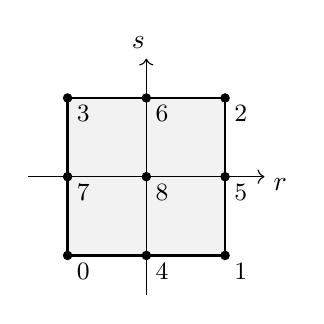
\begin{tikzpicture}
%\draw[step=0.5cm,gray,very thin] (0,0) grid (4,4); 
\draw[fill=gray!10,gray!10](1,1) rectangle (3,3);
\draw[thick] (1,1)--(3,1)--(3,3)--(1,3)--cycle;
\draw [->] (0.5,2) -- (3.5,2);
\draw [->] (2,0.5) -- (2,3.5);
\node[] at (3.7,1.9) {$r$};
\node[] at (1.9,3.7) {$s$};
\draw[black,fill=black] (1,1)   circle (1.5pt);
\draw[black,fill=black] (1,2)   circle (1.5pt);
\draw[black,fill=black] (1,3)   circle (1.5pt);
\draw[black,fill=black] (2,1)   circle (1.5pt);
\draw[black,fill=black] (2,2)   circle (1.5pt);
\draw[black,fill=black] (2,3)   circle (1.5pt);
\draw[black,fill=black] (3,1)   circle (1.5pt);
\draw[black,fill=black] (3,2)   circle (1.5pt);
\draw[black,fill=black] (3,3)   circle (1.5pt);
\node[] at (1.2,0.8) {\small $0$};
\node[] at (2.2,0.8) {\small $4$};
\node[] at (3.2,0.8) {\small $1$};
\node[] at (1.2,1.8) {\small $7$};
\node[] at (2.2,1.8) {\small $8$};
\node[] at (3.2,1.8) {\small $5$};
\node[] at (1.2,2.8) {\small $3$};
\node[] at (2.2,2.8) {\small $6$};
\node[] at (3.2,2.8) {\small $2$};
\end{tikzpicture}
\end{center}



\[
\vec{\bN}(r,s) 
=
\left(
\begin{array}{c}
\bN_1(r,s) \\ 
\bN_2(r,s) \\
\bN_3(r,s) \\
\bN_4(r,s) \\
\bN_5(r,s) \\
\bN_6(r,s) \\
\bN_7(r,s) \\
\bN_8(r,s) \\
\bN_9(r,s) 
\end{array}
\right)
=
\left(
\begin{array}{c}
\bN_1(r) \bN_1(s) \\
\bN_2(r) \bN_1(s) \\
\bN_3(r) \bN_1(s) \\
\bN_1(r) \bN_2(s) \\
\bN_2(r) \bN_2(s) \\
\bN_3(r) \bN_2(s) \\
\bN_1(r) \bN_3(s) \\
\bN_2(r) \bN_3(s) \\
\bN_3(r) \bN_3(s) 
\end{array}
\right)
=
\left(
\begin{array}{c}
 \frac{1}{2}r(r-1)  \frac{1}{2}s(s-1)\\
     (1-r^2)        \frac{1}{2}s(s-1)\\
 \frac{1}{2}r(r+1)  \frac{1}{2}s(s-1)\\
 \frac{1}{2}r(r-1)  (1-s^2)\\
     (1-r^2)        (1-s^2)
 \frac{1}{2}r(r+1)  (1-s^2)\\
 \frac{1}{2}r(r-1)  \frac{1}{2}s(s+1)\\
     (1-r^2)        \frac{1}{2}s(s+1)\\
 \frac{1}{2}r(r+1)  \frac{1}{2}s(s+1)\\
\end{array}
\right)
\]
The mass matrix on the reference element is then
\[
{\bm M}^e =
\iint_\square
\left(
\begin{array}{ccccccccc}
\bN_1 \bN_1 & \bN_1 \bN_2 & \bN_1 \bN_3 & \bN_1 \bN_4 & \bN_1 \bN_5 & \bN_1 \bN_6 & \bN_1 \bN_7 & \bN_1 \bN_8 & \bN_1 \bN_9 \\ 
\bN_2 \bN_1 & \bN_2 \bN_2 & \bN_2 \bN_3 & \bN_2 \bN_4 & \bN_2 \bN_5 & \bN_2 \bN_6 & \bN_2 \bN_7 & \bN_2 \bN_8 & \bN_2 \bN_9 \\ 
\dots \\
\bN_9 \bN_1 & \bN_9 \bN_2 & \bN_9 \bN_3 & \bN_9 \bN_4 & \bN_9 \bN_5 & \bN_9 \bN_6 & \bN_9 \bN_7 & \bN_9 \bN_8 & \bN_9 \bN_9 
\end{array}
\right)
dr ds
\]
with for example\footnote{Thank you WolframAlpha again!}
\begin{eqnarray}
\iint_\square \bN_1(r,s) \bN_1(r,s) \; drds &=&  \frac{16}{225} \\
\iint_\square \bN_1(r,s) \bN_2(r,s) \; drds &=& \frac{8}{225} \\ 
\iint_\square \bN_1(r,s) \bN_3(r,s) \; drds &=&  -\frac{4}{225} \\
\iint_\square \bN_1(r,s) \bN_8(r,s) \; drds &=&  \frac{-2}{225} \\
\iint_\square \bN_1(r,s) \bN_9(r,s) \; drds &=&  \frac{1}{225} \\
\iint_\square \bN_5(r,s) \bN_5(r,s) \; drds &=&  \frac{256}{225} \\
\end{eqnarray}

In \stone~107, we find for a 3x2 mesh on domain 6x4:
\begin{verbatim}
M = 
[[ 16.   8.  -4.   8.   4.  -2.  -4.  -2.   1.]
 [  8.  64.   8.   4.  32.   4.  -2. -16.  -2.]
 [ -4.   8.  16.  -2.   4.   8.   1.  -2.  -4.]
 [  8.   4.  -2.  64.  32. -16.   8.   4.  -2.]
 [  4.  32.   4.  32. 256.  32.   4.  32.   4.]
 [ -2.   4.   8. -16.  32.  64.  -2.   4.   8.]
 [ -4.  -2.   1.   8.   4.  -2.  16.   8.  -4.]
 [ -2. -16.  -2.   4.  32.   4.   8.  64.   8.]
 [  1.  -2.  -4.  -2.   4.   8.  -4.   8.  16.]] / 225
\end{verbatim}







\newpage
%------------------------------------------------------------------------
\section{3d hexahedra}

%---------------------------
\subsection{Linear cuboid elements $Q_1$ - $\K$ and $\G$ matrices}

We here assume that each element is a cuboid\footnote{\url{https://en.wikipedia.org/wiki/Cuboid}}. 
We set the domain size to $L_x=4$, $L_x=3$ and $L_z=2$, with $nelx=4$, 
$nely=3$ and $nelz=2$. Here again the viscosity is set to $\eta=1$ so that 
we find that 
\begin{footnotesize}
\[
\K_{el}=\frac{1}{8\cdot 9}
\left(
\begin{array}{cccccccccccccccccccccccc}
32&   6&   6&  -8&  -6&  -6& -10&  -6&  -3&   4&   6&   3&   4&   3&    6& -10&  -3&  -6&  -8&  -3&  -3&  -4&   3&   3\\
 6&  32&   6&   6&   4&   3&  -6& -10&  -3&  -6&  -8&  -6&   3&   4&    6&   3&  -4&   3&  -3&  -8&  -3&  -3& -10&  -6\\
 6&   6&  32&   6&   3&   4&   3&   3&  -4&   3&   6&   4&  -6&  -6&   -8&  -6&  -3& -10&  -3&  -3&  -8&  -3&  -6& -10\\
-8&   6&   6&  32&  -6&  -6&   4&  -6&  -3& -10&   6&   3& -10&   3&    6&   4&  -3&  -6&  -4&  -3&  -3&  -8&   3&   3\\
-6&   4&   3&  -6&  32&   6&   6&  -8&  -6&   6& -10&  -3&  -3&  -4&    3&  -3&   4&   6&   3& -10&  -6&   3&  -8&  -3\\
-6&   3&   4&  -6&   6&  32&  -3&   6&   4&  -3&   3&  -4&   6&  -3&  -10&   6&  -6&  -8&   3&  -6& -10&   3&  -3&  -8\\
10&  -6&   3&   4&   6&  -3&  32&   6&  -6&  -8&  -6&   6&  -8&  -3&    3&  -4&   3&  -3&   4&   3&  -6& -10&  -3&   6\\
-6& -10&   3&  -6&  -8&   6&   6&  32&  -6&   6&   4&  -3&  -3&  -8&    3&  -3& -10&   6&   3&   4&  -6&   3&  -4&  -3\\
-3&  -3&  -4&  -3&  -6&   4&  -6&  -6&  32&  -6&  -3&   4&   3&   3&   -8&   3&   6& -10&   6&   6&  -8&   6&   3& -10\\
 4&  -6&   3& -10&   6&  -3&  -8&   6&  -6&  32&  -6&   6&  -4&  -3&    3&  -8&   3&  -3& -10&   3&  -6&   4&  -3&   6\\
 6&  -8&   6&   6& -10&   3&  -6&   4&  -3&  -6&  32&  -6&   3& -10&    6&   3&  -8&   3&  -3&  -4&  -3&  -3&   4&  -6\\
 3&  -6&   4&   3&  -3&  -4&   6&  -3&   4&   6&  -6&  32&  -3&   6&  -10&  -3&   3&  -8&  -6&   3& -10&  -6&   6&  -8\\
 4&   3&  -6& -10&  -3&   6&  -8&  -3&   3&  -4&   3&  -3&  32&   6&   -6&  -8&  -6&   6& -10&  -6&   3&   4&   6&  -3\\
 3&   4&  -6&   3&  -4&  -3&  -3&  -8&   3&  -3& -10&   6&   6&  32&   -6&   6&   4&  -3&  -6& -10&   3&  -6&  -8&   6\\
 6&   6&  -8&   6&   3& -10&   3&   3&  -8&   3&   6& -10&  -6&  -6&   32&  -6&  -3&   4&  -3&  -3&  -4&  -3&  -6&   4\\
10&   3&  -6&   4&  -3&   6&  -4&  -3&   3&  -8&   3&  -3&  -8&   6&   -6&  32&  -6&   6&   4&  -6&   3& -10&   6&  -3\\
-3&  -4&  -3&  -3&   4&  -6&   3& -10&   6&   3&  -8&   3&  -6&   4&   -3&  -6&  32&  -6&   6&  -8&   6&   6& -10&   3\\
-6&   3& -10&  -6&   6&  -8&  -3&   6& -10&  -3&   3&  -8&   6&  -3&    4&   6&  -6&  32&   3&  -6&   4&   3&  -3&  -4\\
-8&  -3&  -3&  -4&   3&   3&   4&   3&   6& -10&  -3&  -6& -10&  -6&   -3&   4&   6&   3&  32&   6&   6&  -8&  -6&  -6\\
-3&  -8&  -3&  -3& -10&  -6&   3&   4&   6&   3&  -4&   3&  -6& -10&   -3&  -6&  -8&  -6&   6&  32&   6&   6&   4&   3\\
-3&  -3&  -8&  -3&  -6& -10&  -6&  -6&  -8&  -6&  -3& -10&   3&   3&   -4&   3&   6&   4&   6&   6&  32&   6&   3&   4\\
-4&  -3&  -3&  -8&   3&   3& -10&   3&   6&   4&  -3&  -6&   4&  -6&   -3& -10&   6&   3&  -8&   6&   6&  32&  -6&  -6\\
 3& -10&  -6&   3&  -8&  -3&  -3&  -4&   3&  -3&   4&   6&   6&  -8&   -6&   6& -10&  -3&  -6&   4&   3&  -6&  32&   6\\
 3&  -6& -10&   37  -3&  -8&   6&  -3& -10&   6&  -6&  -8&  -3&   6&    4&  -3&   3&  -4&  -6&   3&   4&  -6&   6&  32
\end{array}
\right)
\]
\end{footnotesize}
and 
\begin{scriptsize}
\[
\G_{el}=\frac{1}{2\cdot 9}
\left(
\begin{array}{c}
 1\\
 1\\
 1\\
-1\\
 1\\
 1\\
-1\\
-1\\
 1\\
 1\\
-1\\
 1\\
 1\\
 1\\
-1\\
-1\\
 1\\
-1\\
-1\\
-1\\
-1\\
 1\\
-1\\
-1
\end{array}
\right)
\]
\end{scriptsize}


\newpage
%---------------------------------------
\section{Triangles: linear elements} \label{ss:tle}


\subsection{linear elements $P_1$} 

We start from the linear basis functions in the reference triangle given as a function of $r,s$:
\begin{eqnarray}
\bN_1(r,s) &=& 1-r-s \nn\\
\bN_2(r,s) &=& r \nn\\
\bN_3(r,s) &=& s \nn
\end{eqnarray}
and their derivatives:
\begin{eqnarray}
\partial_r \bN_1(r,s) &=& -1 \nonumber\\
\partial_r \bN_2(r,s) &=& 1 \nonumber\\
\partial_r \bN_3(r,s) &=& 0 \nonumber\\
\partial_s \bN_1(r,s) &=& -1 \nonumber\\
\partial_s \bN_2(r,s) &=& 0\nonumber\\
\partial_s \bN_3(r,s) &=& 1\nonumber
\end{eqnarray}
We wish to compute the integral of a function $f(x,y)$ over the triangle by means of a change of variables
$(x,y)\rightarrow (r,s)$:
\begin{eqnarray}
\iint f(x,y) dx dy 
&=& \iint f(x(r,s),y(r,s)) \left| \frac{\partial (x,y)}{\partial (r,s) } \right|  dr ds \nonumber\\
&=& \iint f(x(r,s),y(r,s)) 
\left| 
\begin{array}{cc}
\partial x/\partial r & \partial x/\partial s \\ \\
\partial y/\partial r & \partial y/\partial s 
\end{array}
\right|  dr ds 
\end{eqnarray}
From 
\begin{eqnarray}
x(r,s)&=&\sum_{i=1}^3 \bN_i(r,s) x_i = (1-r-s)x_1 + rx_2 + sx_3 = (x_2-x_1)r+(x_3-x_1)s+x_1  \nn\\
y(r,s)&=&\sum_{i=1}^3 \bN_i(r,s) y_i = (1-r-s)y_1 + ry_2 + sy_3 = (y_2-y_1)r+(y_3-y_1)s+y_1  \nn
\end{eqnarray}
we can write
\begin{eqnarray}
\frac{\partial x}{\partial r}(r,s)
&=&\sum_{i=1}^3 \frac{\partial \bN_i}{\partial r} x_i
=\frac{\partial \bN_1}{\partial r} x_1+\frac{\partial \bN_2}{\partial r} x_2+\frac{\partial \bN_3}{\partial r} x_3
=- x_1+ x_2 \nonumber\\
\frac{\partial x}{\partial s}(r,s)
&=&\sum_{i=1}^3 \frac{\partial \bN_i}{\partial s} x_i
=\frac{\partial \bN_1}{\partial s} x_1+\frac{\partial \bN_2}{\partial s} x_2+\frac{\partial \bN_3}{\partial s} x_3
=- x_1+ x_3
\nonumber\\
\frac{\partial y}{\partial r}(r,s)
&=&\sum_{i=1}^3 \frac{\partial \bN_i}{\partial r} y_i
=\frac{\partial \bN_1}{\partial r} x_1+\frac{\partial \bN_2}{\partial r} x_2+\frac{\partial \bN_3}{\partial r} y_3
=- y_1+ y_2
\nonumber\\
\frac{\partial y}{\partial s}(r,s)
&=&\sum_{i=1}^3 \frac{\partial \bN_i}{\partial s} y_i
=\frac{\partial \bN_1}{\partial s} y_1+\frac{\partial \bN_2}{\partial s} y_2+\frac{\partial \bN_3}{\partial s} y_3
=- y_1+ y_3
\end{eqnarray}
Then 
\[
\left| 
\begin{array}{cc}
\partial x/\partial r & \partial x/\partial s \\ \\
\partial y/\partial r & \partial y/\partial s 
\end{array}
\right|  
=
\left| 
\begin{array}{cc}
- x_1+ x_2 & - x_1+ x_3 \\
- y_1+ y_2 & - y_1+ y_3 
\end{array}
\right|  
=
(x_2-x_1)(y_3-y_1)-(y_2-y_1)(x_3-x_1)
= 2S
\]
where $S$ is the area of the triangle and which is independent of $(r,s)$.
Looking at the reference element, we find that when $r$ goes from 0 to 1, 
$s$ can only take values between 0 and $1-r$.
\begin{center}
\includegraphics[width=4cm]{images/elemental_mat/triangle}
\end{center}
Then the bounds of the integrals are simply: 
\begin{eqnarray}
\iint_\triangle f(x,y) dx dy &=& 2S \int_0^{1} \left(\int_0^{1-r} f(x(r,s),y(r,s))  ds \right) dr 
\end{eqnarray}
and the mass matrix is given by
\begin{eqnarray}
{\bm M}_e 
&=& 2S \int_{0}^1 \left[ \int_{0}^{1-r}
\left(
\begin{array}{ccc}
(1-r-s)^2 & (1-r-s)r & (1-r-s)s \\
(1-r-s)r & r^2 & rs \\
(1-r-s)s & rs & s^2 
\end{array}
\right)
 ds \right] dr \\
&=& 
2S \int_{0}^1 
\left(
\begin{array}{ccc}
\int_0^{1-r} (1-r-s)^2 ds &\int_0^{1-r} (1-r-s)r ds& \int_0^{1-r} (1-r-s)s ds \\ \\
\int_0^{1-r} (1-r-s)r ds  &\int_0^{1-r} r^2 ds     & \int_0^{1-r} rs ds \\ \\
\int_0^{1-r} (1-r-s)s ds  &\int_0^{1-r} rs ds      & \int_0^{1-r} s^2 ds
\end{array}
\right)
 dr \\
&=& 
2S
\left(
\begin{array}{ccc}
1/12 & 1/24 & 1/24 \\
1/24 & 1/12 & 1/24 \\
1/24 & 1/24 & 1/12
\end{array}
\right)
\\
&=&
\frac{S}{12}
\left(
\begin{array}{ccc}
2 & 1 & 1 \\
1 & 2 & 1 \\
1 & 1 & 2
\end{array}
\right)
\end{eqnarray}
This is Eq.(4.10e) of \textcite{li06}. 
Also note that in the context of the heat transport equation this matrix is multiplied 
by $\rho C_p$ (all under the assumption that these coefficients are constant 
over the whole element).

%We will then compute the ${\bm J}_x$ and ${\bm J}_y$ matrices\footnote{Nobody 
%knows what these matrices are for ... needs to be looked into.}.
The basis functions can also directly be expressed in the $(x,y)$ coordinate system
(see for example Section~\ref{ss:p1}):
\begin{eqnarray}
\bN_1(x,y) &=& \frac{1}{2S} \left( x_2y_3-x_3y_2+(y_2-y_3)x+(x_3-x_2)y   \right) \nn\\
\bN_2(x,y) &=& \frac{1}{2S} \left( x_3y_1-x_1y_3+(y_3-y_1)x+(x_1-x_3)y   \right) \nn\\
\bN_3(x,y) &=& \frac{1}{2S} \left( x_1y_2-x_2y_1+(y_1-y_2)x+(x_2-x_1)y   \right) \nn
\end{eqnarray}
where $S$ is the area of the element.
We then have 
\begin{eqnarray}
\partial_x \bN_1(x,y) &=& \frac{1}{2S}  (y_2-y_3) = \frac{1}{2S} y_{23} \nn\\
\partial_x \bN_2(x,y) &=& \frac{1}{2S}  (y_3-y_1) = \frac{1}{2S} y_{31} \nn\\
\partial_x \bN_3(x,y) &=& \frac{1}{2S}  (y_1-y_2) = \frac{1}{2S} y_{12} \nn\\
\partial_y \bN_1(x,y) &=& \frac{1}{2S}  (x_3-x_2) = \frac{1}{2S} y_{32} \nn\\
\partial_y \bN_2(x,y) &=& \frac{1}{2S}  (x_1-x_3) = \frac{1}{2S} y_{13} \nn\\
\partial_y \bN_3(x,y) &=& \frac{1}{2S}  (x_2-x_1) = \frac{1}{2S} y_{21} \nn
\end{eqnarray}
where we have introduced the notation $x_{ij}=x_i-x_j$ and $y_{ij}=y_i-y_j$.

%We start with
%\begin{eqnarray}
%{\bm J}_x
%&=& \iint_\triangle  \partial_x \vec{\bN}^T \vec{\bN} dV \nn\\
%&=&  \iint_\triangle 
%\left(
%\begin{array}{c}
%\frac{1}{2S}(y_2-y_3) \\
%\frac{1}{2S}(y_3-y_1) \\
%\frac{1}{2S}(y_1-y_2)
%\end{array}
%\right)
%\left(
%\begin{array}{ccc}
%N_1(x,y) & N_2(x,y) & N_3(x,y) 
%\end{array}
%\right) dx dy \nn\\
%&=& \frac{1}{2S} 
%\left(
%\begin{array}{ccc}
%y_{23} \iint_\triangle \bN_1 dx dy & y_{23} \iint_\triangle \bN_2 dx dy & y_{23} \iint_\triangle \bN_3 dx dy \\
%y_{31} \iint_\triangle \bN_1 dx dy & y_{31} \iint_\triangle \bN_2 dx dy & y_{31} \iint_\triangle \bN_3 dx dy \\
%y_{12} \iint_\triangle \bN_1 dx dy & y_{12} \iint_\triangle \bN_2 dx dy & y_{12} \iint_\triangle \bN_3 dx dy 
%\end{array}
%\right) 
%\end{eqnarray}
%We then need to compute
%\begin{eqnarray}
%\iint_\triangle \bN_1(x,y) dx dy 
%&=& 2S \int_0^{1} \left(\int_0^{1-r} \bN_1(x(r,s),y(r,s))  ds \right) dr \nonumber\\ 
%&=& 2S \int_0^{1} \left(\int_0^{1-r} (1-r-s)  ds \right) dr \nonumber\\ 
%&=& 2S \frac{1}{6} \label{eq:elmats:1}\\ 
%\iint_\triangle \bN_2(x,y) dx dy 
%&=& 2S \int_0^{1} \left(\int_0^{1-r} \bN_2(x(r,s),y(r,s))  ds \right) dr \nonumber\\ 
%&=& 2S \int_0^{1} \left(\int_0^{1-r} r  ds \right) dr \nonumber\\ 
%&=& 2S \frac{1}{6} \label{eq:elmats:2}\\ 
%\iint_\triangle \bN_3(x,y) dx dy 
%&=& 2S \int_0^{1} \left(\int_0^{1-r} \bN_3(x(r,s),y(r,s))  ds \right) dr \nonumber\\ 
%&=& 2S \int_0^{1} \left(\int_0^{1-r} s  ds \right) dr \nonumber\\ 
%&=& 2S \frac{1}{6} \label{eq:elmats:3} 
%\end{eqnarray}
%\todo[inline]{verify!! FOR REAL 2025}
%Finally:
%\[
%{\bm J}_x
%=
%\frac{1}{6}
%%\left(
%\begin{array}{ccc}
%y_{23} & y_{23} & y_{23} \\ 
%y_{31} & y_{31} & y_{31} \\ 
%y_{12} & y_{12} & y_{12}  
%\end{array}
%\right) 
%\]
%Likewise
%\begin{eqnarray}
%{\bm J}_y
%&=& \iint_\triangle  \partial_y \vec{\bN}^T \vec{\bN} dV \nn\\
%&=&  \iint_\triangle 
%\left(
%\begin{array}{c}
%\frac{1}{2S}(x_3-x_2) \\
%\frac{1}{2S}(x_1-x_3) \\
%\frac{1}{2S}(x_2-x_1)
%\end{array}
%\right)
%\left(
%\begin{array}{ccc}
%\bN_1(x,y) & \bN_2(x,y) & \bN_3(x,y) 
%\end{array}
%\right) dx dy \nn\\
%&=&
%\frac{1}{6}
%\left(
%\begin{array}{ccc}
%x_{32} & x_{32} & x_{32} \\ 
%x_{13} & x_{13} & x_{13} \\ 
%x_{21} & x_{21} & x_{21}  
%\end{array}
%\right) 
%\end{eqnarray}

We now turn to the diffusion $\K_d$ matrices.
The gradient matrix ${\bm B}$ is given by 
\[
{\bm B} = 
\left(
\begin{array}{ccc}
\partial_x \bN_1 & \partial_x \bN_2 & \partial_x \bN_3 \\
\partial_y \bN_1 & \partial_y \bN_2 & \partial_y \bN_3 \\
\end{array}
\right)
=
\frac{1}{2S}
\left(
\begin{array}{ccc}
y_{23} & y_{31} & y_{12} \\
x_{32} & x_{13} & x_{21}
\end{array}
\right)
\]
then 
\[
{\bm K}_d 
= \iint_\triangle {\bm B}^T k {\bm B} \; dV
= \iint_\triangle \frac{k}{4S^2}
\left(
\begin{array}{cc}
y_{23} & x_{32} \\ 
y_{31} & x_{13} \\
y_{12} & x_{21}
\end{array}
\right)
\cdot
\left(
\begin{array}{ccc}
y_{23} & y_{31} & y_{12} \\
x_{32} & x_{13} & x_{21}
\end{array}
\right)
\; dV
\]
If the heat conductivity $k$ is constant within the element, then 
the integrand in the expression above is constant with respect to the 
integration and since $\iint_\triangle dV = S$ we then obtain:
\[
\K_d 
= \frac{k}{4S}
\left(
\begin{array}{cc}
y_{23} & x_{32} \\ 
y_{31} & x_{13} \\
y_{12} & x_{21}
\end{array}
\right)
\cdot
\left(
\begin{array}{ccc}
y_{23} & y_{31} & y_{12} \\
x_{32} & x_{13} & x_{21}
\end{array}
\right)
\]
or
\[
\boxed{
\K_d 
= \frac{k}{4S}
\left(
\begin{array}{ccc}
y_{23}y_{23} + x_{32}x_{32} & y_{23}y_{31} + x_{32}x_{13} & y_{23}y_{12} + x_{32}x_{21}  \\ 
y_{31}y_{23} + x_{13}x_{32} & y_{31}y_{31} + x_{13}x_{13} & y_{31}y_{12} + x_{13}x_{21}  \\ 
y_{12}y_{23} + x_{21}x_{32} & y_{12}y_{31} + x_{21}x_{13} & y_{12}y_{12} + x_{21}x_{21} 
\end{array}
\right)
}
\]



Turning now to the advection matrix
\begin{eqnarray}
\K_a 
&=& \iint_\triangle \vec{\bN}^T  \; \vec{\upnu}\cdot {\bm B} \; dV \nn\\
&=& \iint_\triangle \vec{\bN}^T(x,y) \; \vec{\upnu}(x,y) \cdot {\bm B}(x,y) \; dx dy \nn
\end{eqnarray}

If the velocity is constant within the element (which is rarely the case) then 
this expression can be integrated exactly. If not, a quadrature rule must be used.

Let us assume that velocity is indeed constant inside the element. Then
$\vec{\upnu}(x,y)=\vec\upnu_0=(u_0,v_0)$ and
\begin{eqnarray}
\K_a 
&=& \iint_\triangle \vec{\bN}^T(x,y) \; \vec{\upnu}_0 \cdot {\bm B}(x,y) \; dx dy \nn\\
&=& \iint_\triangle
\left(
\begin{array}{c}
\bN_1(x,y) \\
\bN_2(x,y) \\
\bN_3(x,y) 
\end{array}
\right)
\;
(u_0,v_0)
\cdot
\frac{1}{2S}
\left(
\begin{array}{ccc}
y_{23} & y_{31} & y_{12} \\
x_{32} & x_{13} & x_{21}
\end{array}
\right) \; dxdy \nn\\
&=& 
\frac{1}{2S}
\iint_\triangle
\left(
\begin{array}{c}
\bN_1(x,y) \\
\bN_2(x,y) \\
\bN_3(x,y) 
\end{array}
\right)
\left(
\begin{array}{ccc}
u_0 y_{23}+ v_0 x_{32}  &
u_0 y_{31}+ v_0 x_{13}  &
u_0 y_{12}+ v_0 x_{21}  
\end{array}
\right)
\; dx dy \nn
\end{eqnarray}
Since the terms in the second vector is independent of $x,y$ we will need to compute
\[
\iint_\triangle \bN_1(x,y) dxdy, \qquad 
\iint_\triangle \bN_2(x,y) dxdy, \qquad \text{and} \quad 
\iint_\triangle \bN_3(x,y) dxdy. 
\]
We have established that for any function $f(x,y)$ we have
\[
\iint_\triangle f(x,y) dx dy = 2S \int_0^{1} \left(\int_0^{1-r} f(x(r,s),y(r,s))  ds \right) dr 
\]
Then
\begin{eqnarray}
\iint_\triangle \bN_1(x,y) dxdy 
&=& 2S \int_0^{1} \left(\int_0^{1-r} \bN_1(r,s)  ds \right) dr \nn\\
&=& 2S \int_0^{1} \left(\int_0^{1-r} (1-r-s)  ds \right) dr \nn\\
&=& 2S \int_0^{1} \left[ (1-r)s -\frac12 s^2)   \right]_0^{1-r} dr \nn\\
&=& 2S \int_0^{1} \left( (1-r)^2 -\frac12 (1-r)^2   \right) dr \nn\\
&=& 2S \int_0^{1} \frac12 (1-r)^2  dr \nn\\
&=& 2S \frac16 \nn\\
\iint_\triangle \bN_2(x,y) dxdy 
&=& 2S \int_0^{1} \left(\int_0^{1-r} \bN_2(r,s)  ds \right) dr \nn\\
&=& 2S \int_0^{1} \left(\int_0^{1-r} r  ds \right) dr \nn\\
&=& 2S \int_0^{1} r (1-r) dr \nn\\
&=& 2S \frac16 \nn\\
\iint_\triangle \bN_3(x,y) dxdy 
&=& 2S \int_0^{1} \left(\int_0^{1-r} \bN_3(r,s)  ds \right) dr \nn\\
&=& 2S \int_0^{1} \left(\int_0^{1-r} s  ds \right) dr \nn\\
&=& 2S \int_0^{1} [\frac12 s^2]_0^{1-r}  dr \nn\\
&=& 2S \frac12 \int_0^{1} (1-r)^2  dr \nn\\
&=& 2S \frac16 \nn
\end{eqnarray}
In the end
\[
\boxed{
\K_a
= \frac16
\left(
\begin{array}{ccc}
u_0 y_{23}+ v_0 x_{32}  & u_0 y_{31}+ v_0 x_{13}  & u_0 y_{12}+ v_0 x_{21}  \\
u_0 y_{23}+ v_0 x_{32}  & u_0 y_{31}+ v_0 x_{13}  & u_0 y_{12}+ v_0 x_{21}  \\
u_0 y_{23}+ v_0 x_{32}  & u_0 y_{31}+ v_0 x_{13}  & u_0 y_{12}+ v_0 x_{21}  
\end{array}
\right)
}
\]
This expression was tested against a numerically integrated approach in 
\stone~45 (simply set \lstinline{test=True} in the code). 

If the element under consideration is the reference element, we 
we have

\begin{eqnarray}
\K_a 
&=& 
\int_0^{1} \left[ \int_0^{1-r}
\left(
\begin{array}{c}
\bN_1(r,s) \\
\bN_2(r,s) \\
\bN_3(r,s) 
\end{array}
\right)
\;
(u_0,v_0)
\cdot
\left(
\begin{array}{ccc}
-1 & 1 & 0 \\
-1 & 0 & 1
\end{array}
\right) ds \right] dr  \nn\\
&=&
\int_0^{1} \left[ \int_0^{1-r}
\left(
\begin{array}{c}
\bN_1(r,s) \\
\bN_2(r,s) \\
\bN_3(r,s) 
\end{array}
\right)
(-u_0-v_0 , u_0 , v_0) \;
ds \right] dr \nn\\
&=& \frac16
\left(
\begin{array}{ccc}
-u_0 - v_0   & u_0   &  v_0   \\
-u_0 - v_0   & u_0   &  v_0   \\
-u_0 - v_0   & u_0   &  v_0   
\end{array}
\right)
\end{eqnarray}















\newpage
\[
{\bm C}_1
=\int_{\partial\Omega_1} \vec{N}^T(x,y) \vec{N}(x,y) d\Gamma
\]
The edge $\partial\Omega_1$ is bounded by the coordinates of nodes $x_1,y_1$
and $x_2,y_2$. This segment can be parameterised by $t\in[0,1]$:
\[
\vec{r}(t) = (1-t)\left(\begin{array}{c} x_1 \\ y_1 \end{array} \right) + 
t \left(\begin{array}{c} x_2 \\ y_2 \end{array} \right)
=
\left(\begin{array}{c} (x_2-x_1)t +x_1 \\ (y_2-y_1)t+y_1 \end{array} \right) 
\]

Let us assume that $C$ is a smooth curve and that it is given by the 
parametric equations $x=h(t)$, $y=g(t)$ and $a\leq t \leq b$. The line integral 
of a function $f(x,y)$ over $C$ is computed as follows. 
\[
\int_C f(x,y) ds = \int_a^b f(h(t),g(t)) \sqrt{\left(\frac{dx}{dt}\right)^2 + \left(\frac{dy}{dt}\right)^2} dt
\]
In our case $dx/dt=x_2-x_1$ and $dy/dt=y_2-y_1$ so 
\[
\sqrt{\left(\frac{dx}{dt}\right)^2 + \left(\frac{dy}{dt}\right)^2}
=\sqrt{(x_2-x_1)^2+(y_2-y_1)^2} = L_1
\]
Then 
\begin{eqnarray}
{\bm C}_1
&=&\int_{\partial\Omega_1} \vec{N}^T(x,y) \vec{N}(x,y) d\Gamma \nn\\
&=&
\left(
\begin{array}{ccc}
\int_{\partial\Omega_1} N_1(x,y)N_1(x,y) d\Gamma & 
\int_{\partial\Omega_1} N_1(x,y)N_2(x,y) d\Gamma &
\int_{\partial\Omega_1} N_1(x,y)N_3(x,y) d\Gamma \\
\int_{\partial\Omega_1} N_2(x,y)N_1(x,y) d\Gamma & 
\int_{\partial\Omega_1} N_2(x,y)N_2(x,y) d\Gamma &
\int_{\partial\Omega_1} N_2(x,y)N_3(x,y) d\Gamma \\
\int_{\partial\Omega_1} N_3(x,y)N_1(x,y) d\Gamma & 
\int_{\partial\Omega_1} N_3(x,y)N_2(x,y) d\Gamma &
\int_{\partial\Omega_1} N_3(x,y)N_3(x,y) d\Gamma 
\end{array}
\right) \nn\\
&=&
L_1
\left(
\begin{array}{ccc}
\int_{0}^1 N_1(x(t),y(t))N_1(x(t),y(t)) dt & 
\int_{0}^1 N_1(x(t),y(t))N_2(x(t),y(t)) dt &
\int_{0}^1 N_1(x(t),y(t))N_3(x(t),y(t)) dt \\\\
\int_{0}^1 N_2(x(t),y(t))N_1(x(t),y(t)) dt & 
\int_{0}^1 N_2(x(t),y(t))N_2(x(t),y(t)) dt &
\int_{0}^1 N_2(x(t),y(t))N_3(x(t),y(t)) dt \\\\
\int_{0}^1 N_3(x(t),y(t))N_1(x(t),y(t)) dt & 
\int_{0}^1 N_3(x(t),y(t))N_2(x(t),y(t)) dt &
\int_{0}^1 N_3(x(t),y(t))N_3(x(t),y(t)) dt
\end{array}
\right) \nn\\
\end{eqnarray}

We are about to compute the individual terms of the matrix
one by one but we will need:
\begin{eqnarray}
S
&=& \frac{1}{2} [(x_1-x_3)(y_2-y_3)-(x_2-x_3)(y_1-y_3)]  \nn\\
&=&  \frac{1}{2} [x_1y_2 -x_1y_3 -x_3y_2 + x_3y_3 -x_2y_1 + x_2y_3 + x_3y_1 - x_3y_3] \nn\\
&=&  \frac{1}{2} [x_1y_2 -x_1y_3 -x_3y_2 -x_2y_1 + x_2y_3 + x_3y_1 ] \nn\\
\end{eqnarray}
and 
\begin{eqnarray}
N_1(x(t),y(t)) 
&=&\frac{1}{2S} [  x_2y_3-x_3y_2+(y_2-y_3)x(t)+(x_3-x_2)y(t) ] \nn\\
&=&\frac{1}{2S} [  x_2y_3-x_3y_2+y_{23}(x_{21} t +x_1)  +x_{32}  (y_{21} t+y_1) ] \nn\\
&=&\frac{1}{2S} [ x_2y_3-x_3y_2 +y_{23}x_1+x_{32}y_1 + (y_{23}x_{21}+x_{32}y_{21}) t  ] \nn\\
&=&\frac{1}{2S} [ \underbrace{x_2y_3-x_3y_2 +x_1y_2-x_1y_3 +x_{3}y_1-x_2y_1}_{2S} \\ 
&& + (x_2y_2-x_1y_2-x_2y_3+x_1y_3 + x_3y_2 - x_3y_1 - x_2y_2 + x_2y_1  ) t  ]  \nn\\
&=&\frac{1}{2S} [ 2S - (\underbrace{x_1y_2+x_2y_3-x_1y_3 - x_3y_2 + x_3y_1 - x_2y_1}_{2S}  ) t  ]  \nn\\
&=&\frac{1}{2S} [ 2S - 2S  t  ] \nn\\
&=&1-t \\
N_2(x(t),y(t)) 
&=& \frac{1}{2S} [ x_3y_1-x_1y_3+(y_3-y_1)(x_{21} t +x_1)+(x_1-x_3)(y_{21} t+y_1)  ] \nn\\
&=& \frac{1}{2S} [ x_3y_1-x_1y_3+(y_3-y_1)x_1+(x_1-x_3)y_1 + (y_{31}x_{21}+x_{13}y_{21}) t ] \nn\\
&=& \frac{1}{2S} [ x_3y_1-x_1y_3+x_1y_3 -x_1y_1+ x_1y_1 -x_3y_1 + (y_{31}x_{21}+x_{13}y_{21}) t ] \nn\\
&=& \frac{1}{2S}   (y_{31}x_{21}+x_{13}y_{21}) t  \nn\\
&=& t \\ 
N_3(x(t),y(t)) 
&=& \frac{1}{2S} ( x_1y_2-x_2y_1+(y_1-y_2)x(t)+(x_2-x_1)y(t)   ) \nn\\
&=& \frac{1}{2S} ( x_1y_2-x_2y_1+(y_1-y_2)( x_{21} t +x_1 )+(x_2-x_1)(y_{21} t+y_1 )   ) \nn\\
&=& \frac{1}{2S} ( x_1y_2-x_2y_1+(y_1-y_2)x_1 +(x_2-x_1)y_1 + (y_{12}x_{21}+x_{21}y_{21})t  ) \nn\\
&=& \frac{1}{2S} ( x_1y_2-x_2y_1+x_1y_1-x_1y_2 +x_2y_1-x_1y_1 + (y_{12}x_{21}-x_{21}y_{12})t     ) \nn\\
&=& 0
\end{eqnarray}


then 

\begin{eqnarray}
\int_{0}^1 N_1(x(t),y(t))N_1(x(t),y(t)) dt 
&=& \int_{0}^1 (1-t)^2 dt = 1/3 \\ 
\int_{0}^1 N_1(x(t),y(t))N_2(x(t),y(t)) dt 
&=& \int_{0}^1 (1-t)t dt = 1/6 \\ 
\int_{0}^1 N_1(x(t),y(t))N_3(x(t),y(t)) dt
&=& 0 \\
\int_{0}^1 N_2(x(t),y(t))N_2(x(t),y(t)) dt 
&=& \int_{0}^1 t^2 dt = 1/3 \\ 
\int_{0}^1 N_2(x(t),y(t))N_3(x(t),y(t)) dt
&=& 0 \\
\int_{0}^1 N_3(x(t),y(t))N_3(x(t),y(t)) dt
&=& 0 
\end{eqnarray}
and finally 
\begin{eqnarray}
{\bm C}_1
&=&\int_{\partial\Omega_1} \vec{N}^T(x,y) \vec{N}(x,y) d\Gamma 
= \frac{L_1}{6}
\left(
\begin{array}{ccc}
2 & 1 & 0 \\
1 & 2 & 0 \\
0 & 0 & 0 
\end{array}
\right) \\
{\bm C}_2 &=&\int_{\partial\Omega_2} \vec{N}^T(x,y) \vec{N}(x,y) d\Gamma 
= \frac{L_2}{6}
\left(
\begin{array}{ccc}
0 & 0 & 0 \\
0 & 2 & 1 \\
0 & 1 & 2 
\end{array}
\right) \\
{\bm C}_3 &=&\int_{\partial\Omega_3} \vec{N}^T(x,y) \vec{N}(x,y) d\Gamma 
= \frac{L_3}{6}
\left(
\begin{array}{ccc}
2 & 0 & 1 \\
0 & 0 & 0 \\
1 & 0 & 2 
\end{array}
\right) 
\end{eqnarray}





 %%%%%
\chapter{Finite element terminology in various languages} 
\begin{tabular}{lll}
English                        & French                                 &   Dutch \\
\hline
Finite Element Method          & M{\'e}thode des {\'e}l{\'e}ments finis &                               \\
Matrix                         & Matrice                                &                               \\
Heat transport equation        & Equation de transport de la chaleur    & Warmtetransport vergelijking  \\
Momentum conservation equation & {\'e}quation de conservation du moment &    \\
Mass conservation equation     &                                        &    \\
Iterative solver               & solveur it{\'e}ratif                   &    \\
Elemental matrix               &                                        &    \\
Boundary conditions            & conditions aux limites                 &    \\
(In)compressible               & (in)compressible                       &    \\
Surface processes              & processus de surface                   &    \\
an element                     & un {\'e}l{\'e}ment                     &    \\
Computational geodynamics      & g{\'e}odynamique num{\'e}rique         &    \\
\hline
\end{tabular}
 %%%%%%%%%%%%%%%%%%%%
\chapter{Fun modelling} Because sometimes numerical modelling {\sl is} fun ...

\begin{center}
\includegraphics[width=8cm]{images/interesting/akds14}\\
{\small Clothes washing simulations \cite{akds14}}
\end{center}


\begin{center}
\includegraphics[width=8cm]{images/interesting/mega03}\\
{\small Pressures produced when penguins pooh—calculations on avian defaecation \cite{mega03}}
\end{center}


 %%%%%%%%%%%%%%%%%%%%%%%%%%%%%%%%%%%%%%%%%%%%%%%%%%%%%%%
\chapter{Beautiful/interesting images from computational geodynamics}

\includegraphics[width=5cm]{images/beautiful/zhgt13}
\cite{zhgt13}

\includegraphics[width=5cm]{images/beautiful/stgb10}
\cite{stgb10}
 %%%%%%%%%%%%
\chapter{Working with Git} \textbf{MIND YOURSELF: Working in a Mac OS, be carefull with case sensitive file names etc...}

In this appendix we summarize the most important commands one should and remember while working with github. After creating an account one can 'fork' a repository (repo) in the online environment. This repository is a copy from the master directory of the developer and should not be used to adapt or change, as changes from the developer (updates) should be obtained in this 'fork', or as it could also be called; your master branch. 
  
In order to be able to work within a repository, for instance, to run and compile different programs, you should have you own branch of the repository in which YOU CAN make changes. The following commands should be used to make, copy and publish your own version of the repo to your local device and the online github environment.

\begin{center}
\begin{tabular}{p{6cm}|p{9cm}}
\textbf{command} &  \textbf{what it does} \\
\hline
  git branch & shows all branches of your repository and highlights the one you're in. \\
  git checkout -b \textless my\_own\_branch\textgreater & This makes your own branch called "my\_own\_branch". \\
  git push origin \textless my\_own\_branch\textgreater & This pushes your own, local, branch to as a second branch in the online repo of github. \\
  git checkout \textless name\textgreater & changing the branch your working in (e.g. master or my\_own\_branch). Or replace the name with a hyphen to switch to the last branch.\\
  git branch -d \textless my\_own\_branch\textgreater & Delete your local branch. \\
  \end{tabular}
\end{center}

  The following commands should be used in order to update your own local branches from updates made by somewhere else (upstream/master is the main repository). One should do this for the local master branch and, where possible as well for the different local branches you have committed changes to already. 

  
\begin{center}
\begin{tabular}{p{6cm}|p{9cm}}
\textbf{command} &  \textbf{what it does} \\
\hline
git checkout master & To make sure you are in the right branch \\
  git fetch upstream & to fetch updates from upstream repositories to you own local branch (e.g. to update your master branch. \\
  git merge upstream/master & Command to update the branch with the fethched repo from 'upstream'. \\
  git push origin master & To level your own online repository again with the one on your local drive (and thus the one upstream). \\
  git checkout \textless my\_own\_branch\textgreater & To switch to your own adapted branch of the repo. \\
  git merge master & Used from another branch working directory to combine the new released version of the master repo with the one where all your own changes are put. -\textgreater Then git finds all conflicts in different files which you need to resolve. \\
  git add . & This adds the resolved issues in your own local branch (not master). After which you are able to commit and push your changes back to the online respository. 
\end{tabular}
\end{center}


While you are working in your own branch you can change, add or delete files in any amount you want. However, always check whether your changes do not inflict the outcome of for instance your code. And when uploading from your terminal: if you commit and then push from master branch your changes will automatically be inserted in the online version of your master branch, when done from another branch it will be shown as a pull request towards your master branch. This request can than, for instance be forwarded to the main repo.\\

\begin{center}
\begin{tabular}{p{6cm}|p{9cm}}
\textbf{command} &  \textbf{what it does} \\
\hline
  git commit -a & This will send your changes/updates from your branch as a commit to your own local branch. \\
  git push origin \textless changes\textgreater & To update the remote repository (on Github) from you local repository (in this case the 'changes' branch). (Actually upload the new version). Online one can then judge what to do with it. !! this is a pull request towards your own fork/local\_branch \\ 
  git status & Showing the status of your current branch; it shows which files are different between the master file and your adapted branch. \\
  git diff \textless changes\textgreater& This shows the exact differences between the different branches; one can simply ask for the difference between two branches when pwd in one branch ask for the other branch. \\ 
  git merge \textless my\_own\_branch\textgreater & When used from the master branch (or any other???) this accepts the changes made in your branch and puts them in your local(!) master branch. \\ 
  git pull origin master & if the main repository changes, one can pull the newest version towards it's own master file. While keeping your own branches alive with you own changes and vica versa: by running this command the origin/master (remote file) will be cloned and updated to the working branch you are in. \\
  git stash (apply) & ?? While updating your local branch, sometimes git wants to overrule your own changes, with this command you can 'stash' them to look at the differences later. ?? \\
\end{tabular}
\end{center}

%..............................................
\paragraph{Very concretely, if you wish to contribute:} 

\begin{enumerate}
\item clone/update the last version of fieldstone on your computer
\item create a branch and check it out
\item carry out your modifications (typo, additional reference, new equation, new stone, ... anything, really!)
\item commit and push 
\item go to github.com and click pull request
\end{enumerate}
 %%%%%%%%%%%%%%%%%%%%%%%%%%%%%%%%%%%%%%%%%%%%%%%%%%%%%%%%%
\chapter{Writing a report as homework \label{app:grading}} \begin{flushright} {\tiny {\color{gray} app\_grading.tex}} \end{flushright}
%~~~~~~~~~~~~~~~~~~~~~~~~~~~~~~~~~~~~~~~~~~~~~~~~~~~~~~~~~~~~~~~~~~~~~~~~~~~~~~~~~~~~~~~~~~~~~~~~~~


\begin{itemize}
\item 
The document should contain your full name and student number on the first page. 
\item 
The file should be a pdf which name contains your family name
\item 
Layout: is the document visually pleasing? Is it well structured? 
\item Is there a complete bibliography (when applicable)?
\item Does the structure follows this: Introduction - Methods - Results - Discussion - Conclusion - Appendix ?
\item 
Figures: Are they properly numbered? captioned? all figures must be referenced in the text. 
Are they of good enough quality (no visible pixels)? are they readable? are all axis labelled?
\item 
Text: Overall quality of the language. Are there still typos? Do all sentence make sense?
\item if you wish to show lines of code, use verbatim or lstlisting\footnote{\url{https://en.wikibooks.org/wiki/LaTeX/Source_Code_Listings}} 
\item 
Discussion: are the results properly discussed, analyzed? are potential problems, errors, limitations discussed?
\item 
Conclusion: Are the findings/results summarized and generalized?
\end{itemize}

\begin{center}
\begin{tabular}{cc}
\hline
No & Yes \\
\hline
\hline
$6.67*10^{-11}$ & $6.67 \times 10^{-11}$ \\
$kg/m^3$ &  kg/m$^{3}$ or kg.m$^{-3}$\\
1x1 & 1$\times$1\\
$cos$ & $\cos$\\
docx file & pdf file \\
'if you do this'& passive form \\ 
\hline
\end{tabular}
\end{center}




%.....................................
\par\noindent\rule{\textwidth}{0.4pt}
\begin{center}
\includegraphics[width=10cm]{images/grading/grey}\\
No grey background
\end{center}


%.....................................
\par\noindent\rule{\textwidth}{0.4pt}
\begin{center}
\includegraphics[width=8cm]{images/grading/numbers}\\
No lists/arrays with numbers
\end{center}

%.....................................
\par\noindent\rule{\textwidth}{0.4pt}
\begin{center}
\includegraphics[width=10cm]{images/grading/arrows2}\\
Too many arrows\\
\includegraphics[width=9cm]{images/grading/arrows1}\\
Poor choice of arrow colour
\end{center}

%.....................................
\par\noindent\rule{\textwidth}{0.4pt}
\begin{center}
\includegraphics[width=8cm]{images/grading/pixels1}
\includegraphics[width=7cm]{images/grading/pixels2}\\
Be careful about how you export your figures. These are unreadable.
\end{center}
 
%.....................................
\par\noindent\rule{\textwidth}{0.4pt}
\begin{center}
\includegraphics[width=8cm]{images/grading/eqs1}\\
Parenthesis too small
\end{center}

%.....................................
\par\noindent\rule{\textwidth}{0.4pt}
\begin{center}
\includegraphics[width=9cm]{images/grading/eqs2}\\
1.6E+10 is not acceptable. Replace by $1.6\cdot 10^{10}$
\end{center}

%.....................................
\par\noindent\rule{\textwidth}{0.4pt}
\begin{center}
\includegraphics[width=7cm]{images/grading/eqs3}\\
Equation number is too close to the equation itself. Use labels, 
do not number equations by hand.
\end{center}

%.....................................
\par\noindent\rule{\textwidth}{0.4pt}
\begin{center}
\includegraphics[width=9cm]{images/grading/eqs4}\\
Formatting of both axis lead to unreadable figure.
\end{center}

%.....................................
\par\noindent\rule{\textwidth}{0.4pt}
\begin{center}
\includegraphics[width=9cm]{images/grading/eqs5}\\
In \LaTeX{}  use \verb!\sum\limits!
\end{center}

%.....................................
\par\noindent\rule{\textwidth}{0.4pt}
\begin{center}
\includegraphics[width=9cm]{images/grading/eqs6}\\
Are so many digits necessary?
\end{center}

%.....................................
\par\noindent\rule{\textwidth}{0.4pt}
\begin{center}
\includegraphics[width=10cm]{images/grading/width}\\
use \verb!\usepackage[cm]{fullpage}! to allow for wider text.
\end{center}

%.....................................
\par\noindent\rule{\textwidth}{0.4pt}
\begin{center}
\includegraphics[width=10cm]{images/grading/figs1}\\
This figure style is to be avoided. Simply use dots and/or lines.
\end{center}

%.....................................
\par\noindent\rule{\textwidth}{0.4pt}
\begin{center}
\includegraphics[width=8cm]{images/grading/figs2}
\end{center}

%------------------------------------------------------------
\subsection{Computational Geodynamics Report}

All the comments above apply, with additional instructions:
\begin{itemize}
\item report should be in \LaTeX 
\item The document should contain your full name and student number on the first page. 
\item The report file should be a pdf which name contains your family name
\item not more than 25 pages. If more, use appendices wisely.
\item document should be structured in two main parts: FDM and FEM.
\item no equations unless necessary to the discussion (still mention the equation that 
you are solving but refer to an external document/article/book for example).
\item use lstlisting package to include code
\item use {\verb| \usepackage[cm]{fullpage} |} to format your document
\item all codes either in appendix or in zip file (bearing your name).
\item a decent introduction (half page to one page) which links the topic of this course to geosciences.
\item discussion of results (stability, convergence, influence of resolution, remarks of all kinds).
\item if you did not succeed in doing a particular exercise, please explain what you think the problem is, 
how you know it is not working, etc ...
\item think about colormaps, image compression
\item DEADLINE: July 10th, 2022, 23:59 
\end{itemize}









 %%%%%%%%%%%%%%%%%%%%
\chapter{Analytical expressions for $\G_{el}$} \label{app:Gel} \input{app_Gel} %%%%%%%%%%%%%%%%%%%%
\chapter{Computational Geophysics GEO4-1427 - projects} 

\subsection{Convection in a box *}

This exercise builds on your existing 2D advection-diffusion code. 
Scale up the benchmark described in Section~\ref{sec:ldc_anal} so that 
it runs in a 1000x1000 km domain with Earth-like parameters and velocities
(the maximum velocity is denoted by $\upnu_{conv}$ and will be varied).
Start with an initial zero temperature field and Earth-like boundary conditions 
on the top and bottom, e.g. $T=20$ at the top and $T=1000$ at the bottom. 
Set $k=3$, $C_p=1250$ and $\rho=3000$.

Run the code until steady state is reached. Implement an algorithm which computes the average 
temperature 
\[
<T> = \frac{1}{L_xL_y} \iint T(x,y) dx dy
\]
in the domain and plot it as a function of time.
Also compute the root mean square velocity in the domain:
\[
\upnu_{rms} = \sqrt{   \frac{1}{L_xL_y} \iint (u^2+v^2) dx dy  }
\]
Plot the steady state $<T>$ and $\upnu_{rms} $ as a function of the resolution $h$. 
Plot the temperature on the $x=L_x/2$ line for different values 
of $\upnu_{conv}$.
When possible, make a link with the Mantle Dynamics practical. 

Bonus: Compute and plot the heat flux $\vec{q}=-\vec\nabla T$ in the center of the elements.

%-------------------------------------------
\subsection{Triangular linear elements */**}

Redo the 2D advection-diffusion exercises with triangular elements.
You will need to make a new icon array, and recompute the mass matrix 
and other matrices. The triangular elements are constructed by splitting 
square elements along the diagonal.
See Section~\ref{ss:p1} for the shape functions and their derivatives.
See Appendix~\ref{ss:tle} for the calculations of the matrices.  

%------------------------------------
\subsection{Triangular linear elements ***}

Same exercise as above, with an additional task: run the benchmark
presented in Section~\ref{sec:hfcyl}.
For this you will need to generate a mesh 
such that nodes are placed on the perimeter of the cylinder and there is 
no node inside the cylinder:

\includegraphics[width=8cm]{images/compgeo/hole}

You can build it 
by hand, or you can use an external mesher library.
Vary the heat conduction coefficient to show the effect of diffusion on the obtained
steady state temperature field.  

%---------------------------------------
\subsection{Diffusion of topography ****}

In a 2D plane assign each node an initial topography $h(x,y,t=0)$ given by 
\[
h(x,y,t=0)= h_0 \sin(\pi x/L_x) + \xi(x,y) \delta h
\]
where $L_x$ and $L_y$ are the dimensions of the domain, $h_0$ is the 
height of the orogen, $xi(x,y)$ is a random perturbation in $[-1,1]$
and $\delta h$ is the amplitude of the perturbation.

We wish to 'erode' the topography by means of a (nonlinear) diffusion law
as in section 2.1.1 of Burov \& Cloetingh \cite{bucl97}.

\begin{enumerate}
\item What are the physical parameters needed to carry out this experiment? 
What are the appropriate boundary conditions? 
What is the steady state? What are the relevant time scales? How should we choose the time step?
\item Write a code which solves the linear diffusion equation until steady state is reached.
Explore the effect of $\delta h$. Compute the slope $\vec\nabla h$ inside each element and plot 
its time evolution. 
\item Implement the nonlinear diffusion law and run the model once again. 
\item If a source term is added to the diffusion equation it is in fact a vertical velocity
($\partial h/\partial t$ has the dimensions of a velocity). Add a source term which generates 
uplift in a symmetric and asymmetric manner.  
\end{enumerate}

\Literature  \cite{thsh14} \cite{ster20}, also check Appendix H. 

%-----------------------------------------------
\subsection{An example of a hand-built triangular mesh}

We start from a 8x5 domain which is tesselated as follows:

\begin{center}
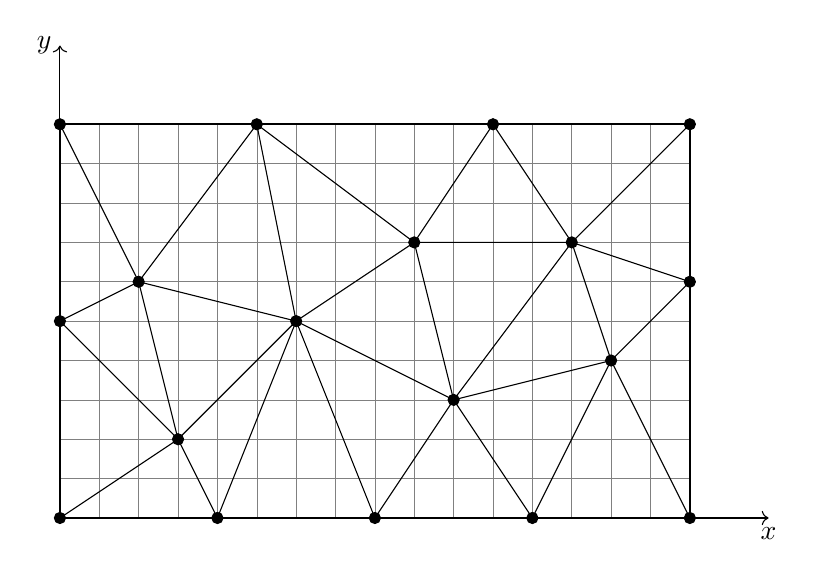
\begin{tikzpicture}
%\draw[fill=gray!8,gray!8](0,0) rectangle (10,7);
\draw[step=0.5cm,gray,very thin] (1,1) grid (9,6); %background grid
\draw[thick] (1,1) -- (9,1) -- (9,6) -- (1,6) -- cycle;  

\draw[thin,->] (1,1) -- (10,1) ; %horizontal axis
\draw[thin,->] (1,1) -- (1,7) ; %horizontal axis
\node[] at (10,0.8){$x$};
\node[] at (0.8,7){$y$};

\draw[] (1,1) -- (2.5,2) -- (4,3.5) -- (5.5,4.5) -- (6.5,6);  %1 6 11 13 14
\draw[] (3,1) -- (4,3.5) -- (6,2.5) -- (7.5,4.5) -- (9,6) ;  %2 11 12 15 16
\draw[] (3,1) -- (2.5,2) -- (1,3.5) -- (2,4) -- (1,6) ;  %2 6 7 8 9
\draw[] (5,1) -- (6,2.5) -- (7,1) -- (8,3) -- (9,4) -- (7.5,4.5) -- (6.5,6) ;  %3 12 4 18 17 15 14
\draw[] (3.5,6) -- (2,4) -- (4,3.5) -- (5,1) ;  %10 8 11 3
\draw[] (2.5,2) -- (2,4) ; %6 8
\draw[] (4,3.5) -- (3.5,6) -- (5.5,4.5) -- (7.5,4.5) ;  %11 10 13 15
\draw[] (9,1) -- (8,3) -- (6,2.5) -- (5.5,4.5) ;  %5 18 12 13
\draw[] (7.5,4.5) -- (8,3) ; %15 18

\draw[black,fill=black] (1,1)     circle (2pt); 
\draw[black,fill=black] (3,1)     circle (2pt); 
\draw[black,fill=black] (5,1)     circle (2pt); 
\draw[black,fill=black] (7,1)     circle (2pt); 
\draw[black,fill=black] (9,1)     circle (2pt); 
\draw[black,fill=black] (2.5,2)   circle (2pt); 
\draw[black,fill=black] (1,3.5)   circle (2pt); 
\draw[black,fill=black] (2,4)     circle (2pt); 
\draw[black,fill=black] (1,6)     circle (2pt); 
\draw[black,fill=black] (3.5,6)   circle (2pt); 
\draw[black,fill=black] (4,3.5)   circle (2pt); 
\draw[black,fill=black] (6,2.5)   circle (2pt); 
\draw[black,fill=black] (5.5,4.5) circle (2pt); 
\draw[black,fill=black] (6.5,6)   circle (2pt); 
\draw[black,fill=black] (7.5,4.5) circle (2pt); 
\draw[black,fill=black] (9,6)     circle (2pt); 
\draw[black,fill=black] (9,4)     circle (2pt); 
\draw[black,fill=black] (8,3)     circle (2pt); 

\end{tikzpicture}\\
\end{center}
         
We can first label the nodes:

\begin{center}
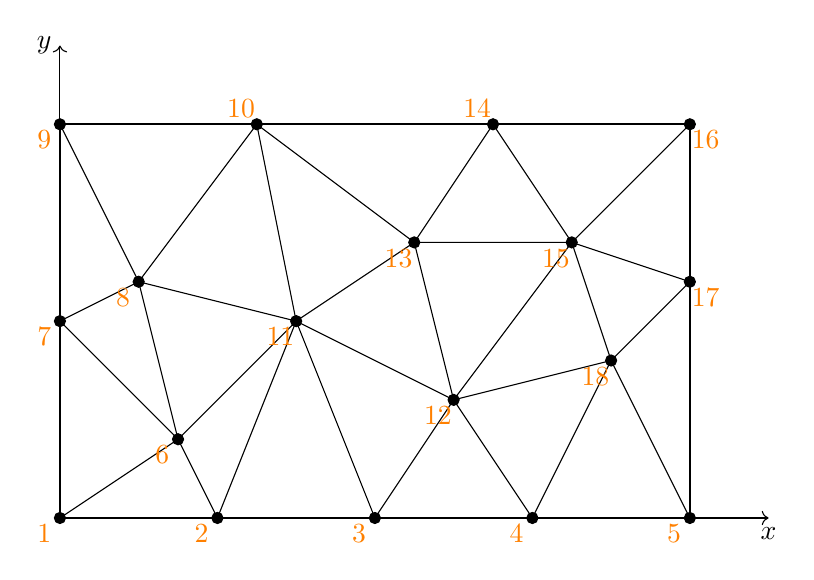
\begin{tikzpicture}
%\draw[fill=gray!5,gray!5](0,0) rectangle (10,7);
%\draw[step=0.5cm,gray,very thin] (1,1) grid (9,6); %background grid
\draw[thick] (1,1) -- (9,1) -- (9,6) -- (1,6) -- cycle;  

\draw[thin,->] (1,1) -- (10,1) ; %horizontal axis
\draw[thin,->] (1,1) -- (1,7) ; %horizontal axis
\node[] at (10,0.8){$x$};
\node[] at (0.8,7){$y$};


\draw[] (1,1) -- (2.5,2) -- (4,3.5) -- (5.5,4.5) -- (6.5,6);  %1 6 11 13 14
\draw[] (3,1) -- (4,3.5) -- (6,2.5) -- (7.5,4.5) -- (9,6) ;  %2 11 12 15 16
\draw[] (3,1) -- (2.5,2) -- (1,3.5) -- (2,4) -- (1,6) ;  %2 6 7 8 9
\draw[] (5,1) -- (6,2.5) -- (7,1) -- (8,3) -- (9,4) -- (7.5,4.5) -- (6.5,6) ;  %3 12 4 18 17 15 14
\draw[] (3.5,6) -- (2,4) -- (4,3.5) -- (5,1) ;  %10 8 11 3
\draw[] (2.5,2) -- (2,4) ; %6 8
\draw[] (4,3.5) -- (3.5,6) -- (5.5,4.5) -- (7.5,4.5) ;  %11 10 13 15
\draw[] (9,1) -- (8,3) -- (6,2.5) -- (5.5,4.5) ;  %5 18 12 13
\draw[] (7.5,4.5) -- (8,3) ; %15 18

\draw[black,fill=black] (1,1)     circle (2pt); \node[] at (0.8,0.8){\color{orange} 1}; %1
\draw[black,fill=black] (3,1)     circle (2pt); \node[] at (2.8,0.8){\color{orange} 2}; %2
\draw[black,fill=black] (5,1)     circle (2pt); \node[] at (4.8,0.8){\color{orange} 3}; %3
\draw[black,fill=black] (7,1)     circle (2pt); \node[] at (6.8,0.8){\color{orange} 4}; %4
\draw[black,fill=black] (9,1)     circle (2pt); \node[] at (8.8,0.8){\color{orange} 5}; %5
\draw[black,fill=black] (2.5,2)   circle (2pt); \node[] at (2.3,1.8){\color{orange} 6}; %6
\draw[black,fill=black] (1,3.5)   circle (2pt); \node[] at (0.8,3.3){\color{orange} 7}; %7
\draw[black,fill=black] (2,4)     circle (2pt); \node[] at (1.8,3.8){\color{orange} 8}; %8
\draw[black,fill=black] (1,6)     circle (2pt); \node[] at (0.8,5.8){\color{orange} 9}; %9
\draw[black,fill=black] (3.5,6)   circle (2pt); \node[] at (3.3,6.2){\color{orange} 10};%10
\draw[black,fill=black] (4,3.5)   circle (2pt); \node[] at (3.8,3.3){\color{orange} 11};%11
\draw[black,fill=black] (6,2.5)   circle (2pt); \node[] at (5.8,2.3){\color{orange} 12};%12
\draw[black,fill=black] (5.5,4.5) circle (2pt); \node[] at (5.3,4.3){\color{orange} 13};%13
\draw[black,fill=black] (6.5,6)   circle (2pt); \node[] at (6.3,6.2){\color{orange} 14};%14
\draw[black,fill=black] (7.5,4.5) circle (2pt); \node[] at (7.3,4.3){\color{orange} 15};%15
\draw[black,fill=black] (9,6)     circle (2pt); \node[] at (9.2,5.8){\color{orange} 16};%16
\draw[black,fill=black] (9,4)     circle (2pt); \node[] at (9.2,3.8){\color{orange} 17};%17
\draw[black,fill=black] (8,3)     circle (2pt); \node[] at (7.8,2.8){\color{orange} 18};%18
\end{tikzpicture}\\
\end{center}

and then label the elements:

\begin{center}
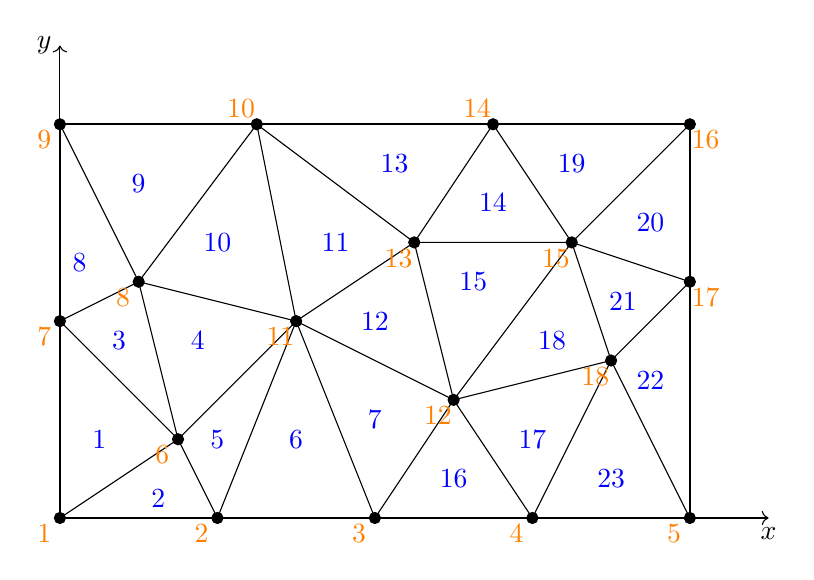
\begin{tikzpicture}
%\draw[fill=gray!5,gray!5](0,0) rectangle (10,7);
%\draw[step=0.5cm,gray,very thin] (1,1) grid (9,6); %background grid
\draw[thick] (1,1) -- (9,1) -- (9,6) -- (1,6) -- cycle;  

\draw[thin,->] (1,1) -- (10,1) ; %horizontal axis
\draw[thin,->] (1,1) -- (1,7) ; %horizontal axis
\node[] at (10,0.8){$x$};
\node[] at (0.8,7){$y$};


\draw[] (1,1) -- (2.5,2) -- (4,3.5) -- (5.5,4.5) -- (6.5,6);  %1 6 11 13 14
\draw[] (3,1) -- (4,3.5) -- (6,2.5) -- (7.5,4.5) -- (9,6) ;  %2 11 12 15 16
\draw[] (3,1) -- (2.5,2) -- (1,3.5) -- (2,4) -- (1,6) ;  %2 6 7 8 9
\draw[] (5,1) -- (6,2.5) -- (7,1) -- (8,3) -- (9,4) -- (7.5,4.5) -- (6.5,6) ;  %3 12 4 18 17 15 14
\draw[] (3.5,6) -- (2,4) -- (4,3.5) -- (5,1) ;  %10 8 11 3
\draw[] (2.5,2) -- (2,4) ; %6 8
\draw[] (4,3.5) -- (3.5,6) -- (5.5,4.5) -- (7.5,4.5) ;  %11 10 13 15
\draw[] (9,1) -- (8,3) -- (6,2.5) -- (5.5,4.5) ;  %5 18 12 13
\draw[] (7.5,4.5) -- (8,3) ; %15 18

\draw[black,fill=black] (1,1)     circle (2pt); \node[] at (0.8,0.8){\color{orange} 1}; %1
\draw[black,fill=black] (3,1)     circle (2pt); \node[] at (2.8,0.8){\color{orange} 2}; %2
\draw[black,fill=black] (5,1)     circle (2pt); \node[] at (4.8,0.8){\color{orange} 3}; %3
\draw[black,fill=black] (7,1)     circle (2pt); \node[] at (6.8,0.8){\color{orange} 4}; %4
\draw[black,fill=black] (9,1)     circle (2pt); \node[] at (8.8,0.8){\color{orange} 5}; %5
\draw[black,fill=black] (2.5,2)   circle (2pt); \node[] at (2.3,1.8){\color{orange} 6}; %6
\draw[black,fill=black] (1,3.5)   circle (2pt); \node[] at (0.8,3.3){\color{orange} 7}; %7
\draw[black,fill=black] (2,4)     circle (2pt); \node[] at (1.8,3.8){\color{orange} 8}; %8
\draw[black,fill=black] (1,6)     circle (2pt); \node[] at (0.8,5.8){\color{orange} 9}; %9
\draw[black,fill=black] (3.5,6)   circle (2pt); \node[] at (3.3,6.2){\color{orange} 10};%10
\draw[black,fill=black] (4,3.5)   circle (2pt); \node[] at (3.8,3.3){\color{orange} 11};%11
\draw[black,fill=black] (6,2.5)   circle (2pt); \node[] at (5.8,2.3){\color{orange} 12};%12
\draw[black,fill=black] (5.5,4.5) circle (2pt); \node[] at (5.3,4.3){\color{orange} 13};%13
\draw[black,fill=black] (6.5,6)   circle (2pt); \node[] at (6.3,6.2){\color{orange} 14};%14
\draw[black,fill=black] (7.5,4.5) circle (2pt); \node[] at (7.3,4.3){\color{orange} 15};%15
\draw[black,fill=black] (9,6)     circle (2pt); \node[] at (9.2,5.8){\color{orange} 16};%16
\draw[black,fill=black] (9,4)     circle (2pt); \node[] at (9.2,3.8){\color{orange} 17};%17
\draw[black,fill=black] (8,3)     circle (2pt); \node[] at (7.8,2.8){\color{orange} 18};%18


\node[] at (1.5,2) {\color{blue}1};
\node[] at (2.25,1.25) {\color{blue}2};
\node[] at (1.75,3.25) {\color{blue}3};
\node[] at (2.75,3.25) {\color{blue}4};
\node[] at (3,2) {\color{blue}5};
\node[] at (4,2) {\color{blue}6};
\node[] at (5,2.25) {\color{blue}7};
\node[] at (1.25,4.25) {\color{blue}8};
\node[] at (2,5.25) {\color{blue}9};
\node[] at (3,4.5) {\color{blue}10};
\node[] at (4.5,4.5) {\color{blue}11};
\node[] at (5,3.5) {\color{blue}12};
\node[] at (5.25,5.5) {\color{blue}13};
\node[] at (6.5,5) {\color{blue}14};
\node[] at (6.25,4) {\color{blue}15};
\node[] at (6,1.5) {\color{blue}16};
\node[] at (7,2) {\color{blue}17};
\node[] at (7.25,3.25) {\color{blue}18};
\node[] at (7.5,5.5) {\color{blue}19};
\node[] at (8.5,4.75) {\color{blue}20};
\node[] at (8.15,3.75) {\color{blue}21};
\node[] at (8.5,2.75) {\color{blue}22};
\node[] at (8,1.5) {\color{blue}23};


\end{tikzpicture}\\
\end{center}

We can finally build the connectivity array by hand:

\noindent
icon(1,{\color{blue}1})={\color{orange}1}\\
icon(2,{\color{blue}1})={\color{orange}6}\\
icon(3,{\color{blue}1})={\color{orange}7}\\
icon(1,{\color{blue}2})={\color{orange}1}\\
icon(2,{\color{blue}2})={\color{orange}2}\\
icon(3,{\color{blue}2})={\color{orange}6}\\
icon(1,{\color{blue}3})={\color{orange}7}\\
icon(2,{\color{blue}3})={\color{orange}6}\\
icon(3,{\color{blue}3})={\color{orange}8}\\
...\\
icon(1,{\color{blue}12})={\color{orange}11}\\
icon(2,{\color{blue}12})={\color{orange}12}\\
icon(3,{\color{blue}12})={\color{orange}13}\\
...\\
icon(1,{\color{blue}19})={\color{orange}14}\\
icon(2,{\color{blue}19})={\color{orange}15}\\
icon(3,{\color{blue}19})={\color{orange}16}\\


The labelling of nodes and elements above is done by a human so it starts at 1. When 
implementing this in python, you know what to do ...


%-----------------------------------------------
\subsection{How to visualise data on a triangular mesh with Paraview}

If arrays {\tt x,y} contain the coordinates of the nodes, your connectivity array is called {\tt icon},
and your mesh consistes of {\tt nel} elements and comprises {\tt nnp} nodes, you can use the following code
to generate a vtu file to be opened with Paraview. You also need a temperature array {\tt T}.

\begin{center}
Code at \url{https://raw.githubusercontent.com/cedrict/fieldstone/master/images/compgeo/mesh_visu.py}
\end{center}

\lstinputlisting[language=python]{images/compgeo/mesh_visu.py}
 %%%%%%%%%%%%%%%%%%%%%%%%%%%
\chapter{Using prisms in forward gravity modelling \label{app:prisms}} 
{\sl This appendix was written by Sverre Hassing as part of his Bachelor thesis.} \index{contributors}{S. Hassing}
Although the final formula are definitely correct, the derivations below may still contain a typo. 

\vspace{.4cm}

The derivations for prisms have been published in the early 50's \cite{made51}. 
However, to the best of our knowledge the full derivation has not been carried out in English in full detail. 
The derivations are based on those of Mader (1951) \cite{made51} and of Nagy \etal (2000) \cite{napb00,napb02}. 
Mader provided the derivations in some detail, while Nagy \etal interpreted the results in a more modern style. 


%----------------------------
\subsection{Basic formulas}

The derivations for prisms are a lot more complicated than that for the point masses. 
We start with the following two integral equations which are integral part of the derivations:

\begin{eqnarray}
\int \frac{x^2 dx}{x^2 + z^2} &=& x - z  \arctan{\frac{x}{z}} \label{eq:basic1} \\
\int \frac{dx}{\sqrt{x^2+y^2+z^2}} &=& \ln{\left( x + \sqrt{x^2+y^2+z^2} \right)} \label{eq:basic2}
\end{eqnarray}
Another equation that will come back multiple times is of the form:
\begin{equation}
\int \frac{du}{(v^2+w^2)\sqrt{u^2+v^2+w^2}}
\end{equation}
This can be solved with a trigonometric substitution, where $u = \sqrt{v^2+w^2} \tan{\phi}$. This means that $du = \frac{\sqrt{v^2+w^2}}{cos^2{\phi}} d\phi$.
\begin{eqnarray}
\int \frac{du}{(v^2+w^2)\sqrt{u^2+v^2+w^2}} 
&=& 
\int \frac{\sqrt{v^2+w^2}}{cos^2{\phi}} 
\frac{1}{(v^2+w^2)\tan^2{\phi}+v^2} 
\frac{d\phi}{\sqrt{v^2+w^2+(v^2+w^2)\tan^2{\phi})}} \nonumber\\
&=& 
\int \frac{\sqrt{v^2+w^2}}{cos{\phi}^2} 
\frac{1}{v^2(\tan^2{\phi}+1) + w^2 \tan^2{\phi}} 
\frac{d\phi}{\sqrt{(v^2+w^2)(\tan^2{\phi}+1)}} \nonumber\\
&=&
\int \frac{\sqrt{v^2+w^2}}{cos{\phi}^2} 
\frac{1}{\frac{v^2+w^2 \sin^2{\phi}}{cos^2{\phi}}} 
\frac{d\phi}{\frac{\sqrt{v^2+w^2}}{cos{\phi}}} \nonumber\\
&=& 
\int \frac{\cos{\phi} d\phi}{v^2+w^2\sin^2{\phi}}
\end{eqnarray}
A second substitution is needed where $t = \frac{w}{v}\sin{\phi}$ and $dt = \frac{v}{w} \cos{\phi} d\phi$:
\begin{eqnarray}
\int \frac{\cos{\phi} d\phi}{v^2+w^2\sin^2{\phi}} 
&=& \int \frac{v dt}{w (v^2+v^2t^2)} \nonumber\\
&=& \frac{1}{vw} \int \frac{dt}{1+t^2} \nonumber\\
&=& \frac{1}{vw} \arctan{t} \nonumber\\
&=& \frac{1}{vw} \arctan{\frac{w \sin{\phi}}{v}} \label{eq:prismbe1}
\end{eqnarray}
Now the $\sin{\phi}$ needs to be converted back to $u,v,w$. If it is known that $\tan{\phi} = \frac{u}{\sqrt{v^2+w^2}}$, then it follows that $\sin{\phi}=\frac{u}{\sqrt{u^2+v^2+w^2}}$.
Eq.\eqref{eq:prismbe1} then becomes
\begin{equation}
{\frac{1}{vw} \arctan \frac{w \sin{\phi}}{v}} = \frac{1}{vw} \arctan{\frac{u w}{v \sqrt{u^2+v^2+w^2}}}
\end{equation}
and finally 
\begin{equation}
\boxed{
\int \frac{du}{(v^2+w^2)\sqrt{u^2+v^2+w^2}} = \frac{1}{vw} \arctan{\frac{u w}{v \sqrt{u^2+v^2+w^2}}} \label{eq:basic3}
}
\end{equation}

\subsection{The gravitational potential}

Each prism is assumed to have constant density $\rho$. The gravitational potential is integrated over the whole volume of the prism:
\begin{equation}
U(P) =  -{\cal G}  \rho \underbrace{\int_{x_1}^{x_2} \int_{y_1}^{y_2} \int_{z_1}^{z_2} \frac{dx dy dz}{\sqrt{x^2+y^2+z^2}}}_{I} \label{eq:der_U_1}
\end{equation}

In what follows we work out the exact form for the triple integral term. Elementary Eq.~\eqref{eq:basic2} can be applied to the integral for $dx$ 
in Eq.~\eqref{eq:der_U_1}.
\begin{eqnarray}
I
&=& \iiint \frac{dx dy dz}{\sqrt{x^2+y^2+z^2}}  \nn\\
&=& \iint \left(\int \frac{dx}{\sqrt{x^2+y^2+z^2}} \right) dydz \nonumber\\
&=& \iint \ln{\left( x+\sqrt{x^2+y^2+z^2} \right)} dy dz
\end{eqnarray}
We further proceed with the integration with respect to $y$. We define
\[
\begin{array}{c|c}
  f = \int \ln{\left( x+\sqrt{x^2+y^2+z^2} \right)} dz 
  & g' = dy \\ 
  \hline
  f' = \frac{y}{\left( x+\sqrt{x^2+y^2+z^2} \right) \sqrt{x^2+y^2+z^2}} 
  & g=y
 \end{array}
\]
and using $\int f g'  = f g - \int f g'$ we have 
\begin{equation}
I= 
\underbrace{y \int \ln{ \left( x + \sqrt{x^2+y^2+z^2} \right) } dz}_{A} 
\underbrace{- \iint  \frac{y^2 dz}{\left( x+\sqrt{x^2+y^2+z^2}\right) \sqrt{x^2+y^2+z^2}} dy}_{B} 
\end{equation}

The calculation of $I$ is then split into two large integrals denoted
$A$ and $B$, calculated in the following subsections.
Note that we have not made use of the integral bounds yet.  

%..................................................................
\subsubsection{The calculation of $A$} \label{subsection:calc_A}

The first step in calculating $A$ is to carry out a similar partial integration as seen before. 

\[
\begin{array}{c|c}
  f=\ln{ \left( x + \sqrt{x^2+y^2+z^2} \right)} & 
  g'=dz \\ 
  \hline
  f' = \frac{\partial f}{\partial z} = \frac{z}{\left( x+\sqrt{x^2+y^2+z^2} \right) \sqrt{x^2+y^2+z^2}} 
  & g = z
 \end{array}
\]

\begin{eqnarray}
A 
&=& 
y \left(z \ln{ \left( x + \sqrt{x^2+y^2+z^2} \right)} - 
\int \frac{z^2 dz}{\left( x+\sqrt{x^2+y^2+z^2} \right) \sqrt{x^2+y^2+z^2}} \right) \nonumber\\
&=& 
\underbrace{yz \ln{ \left( x + \sqrt{x^2+y^2+z^2} \right)} }_{A_0} 
- 
\underbrace{y\int \frac{z^2 dz}{\left( x+\sqrt{x^2+y^2+z^2} \right) \sqrt{x^2+y^2+z^2}}  }_{A_1}
\end{eqnarray}

We now focus on the $A_1$ integral. 
We first multiply the numerator and denominator by $-x+\sqrt{x^2+y^2+z^2} $. The last step uses Eqs.~\eqref{eq:basic2}, \eqref{eq:basic3} and \eqref{eq:basic1} respectively for each term.
\begin{eqnarray}
A_1 
&=& \int \frac{z^2 dz}{\left( x+\sqrt{x^2+y^2+z^2} \right) \sqrt{x^2+y^2+z^2}}
\frac{-x+\sqrt{x^2+y^2+z^2}}{-x+\sqrt{x^2+y^2+z^2}} \nonumber\\
&=& \int \frac{(-x z^2 + z^2 \sqrt{x^2+y^2+z^2} )dz}{\left( x^2+y^2+z^2 - x^2 \right) \sqrt{x^2+y^2+z^2}} \label{eq:der_U_2} \nonumber\\
&=& 
\int \frac{-x z^2 dz}{\left( y^2+z^2  \right) \sqrt{x^2+y^2+z^2}}  
+ \int \frac{z^2 \sqrt{x^2+y^2+z^2} dz}{\left( y^2+z^2  \right) \sqrt{x^2+y^2+z^2}} \nonumber\\
&=& \int \frac{-x \left( z^2 + y^2 -y^2 \right) dz}{(y^2+z^2)\sqrt{x^2+y^2+z^2}} + 
\int \frac{z^2dz}{y^2+z^2} \nonumber\\
&=& \int \frac{-x dz}{\sqrt{x^2+y^2+z^2}} + 
\int \frac{x y^2 dz}{(y^2+z^2)\sqrt{x^2+y^2+z^2}} + 
\int \frac{z^2dz}{y^2+z^2} \nonumber\\
&=& -x \int \frac{ dz}{\sqrt{x^2+y^2+z^2}} + 
x y^2 \int \frac{ dz}{(y^2+z^2)\sqrt{x^2+y^2+z^2}} + 
\int \frac{z^2dz}{y^2+z^2} \nonumber\\
&=& -x \ln{ \left( z + \sqrt{x^2+y^2+z^2} \right)} + 
y \arctan{\frac{x z}{y \sqrt{x^2+y^2+z^2}}} + 
z -  y \arctan{\frac{z}{y}}
\end{eqnarray}
This can be combined to get the final expression for A:
\begin{equation}
A = 
y \left( z \ln{ \left( x + \sqrt{x^2+y^2+z^2} \right)} + 
x \ln{ \left( z + \sqrt{x^2+y^2+z^2} \right)} -  
y \arctan{\frac{x z}{y \sqrt{x^2+y^2+z^2}}} - 
z + 
y \arctan{\frac{z}{y}} \right)
\end{equation}
The last two terms can be left out because they will cancel out when computing the integration boundaries from $x_1$ to $x_2$, because these terms do not contain the variable $x$. 
Finally we arrive at the following expression for $A$:
\begin{equation}
A = 
yz \ln{\left( x + \sqrt{x^2+y^2+z^2} \right)} + 
xy \ln{\left( z + \sqrt{x^2+y^2+z^2} \right)} - 
y^2 \arctan{\frac{xz}{y\sqrt{x^2+y^2+z^2}}}
\end{equation}



%.......................................
\subsubsection{The calculation of $B$}

The inner integral can be simplified similarly to how $A_1$ was simplified in Eq.~\eqref{eq:der_U_2}, 
by multiplying both numerator and denominator with $-x+\sqrt{x^2+y^2+z^2}$. The last step uses Eqs.~\eqref{eq:basic3} and \eqref{eq:basic1}:
\begin{eqnarray}
B 
&=& 
-\int y^2 \int \frac{dz}{\left( x + \sqrt{x^2+y^2+z^2} \right) \sqrt{x^2+y^2+z^2}} 
\frac{-x + \sqrt{x^2+y^2+z^2}}{-x + \sqrt{x^2+y^2+z^2}} dy \nonumber\\
&=& - \int y^2 \int \frac{-x + \sqrt{x^2+y^2+z^2} }{\left( x^2 + y^2+z^2 -x^2 \right) \sqrt{x^2+y^2+z^2}}dz dy \nonumber\\
&=& - \int y^2 \left( 
- \int \frac{x dz}{(y^2+z^2)\sqrt{x^2+y^2+z^2}} +
\int \frac{dz}{y^2+z^2} 
\right) dy \nonumber\\
&=& - \int y^2 \left( -\frac{1}{y} \arctan{\frac{xz}{y\sqrt{x^2+y^2+z^2}}} + \frac{1}{y} \arctan{\frac{z}{y}}\right) dy \nn\\
&=& \int y \arctan{\frac{xz}{y\sqrt{x^2+y^2+z^2}}} dy
\end{eqnarray}
Again the second term can be left out, because it does not contain the variable $x$. The next step is to apply a partial integration to $B$.  

\[
\begin{array}{c|c}
  f=\arctan{\frac{xz}{y\sqrt{x^2+y^2+z^2}}} & g'=y \\ 
  \hline
  f' = -xz \frac{\frac{1}{y^2 \sqrt{x^2+y^2+z^2}}+\frac{1}{(x^2+y^2+z^2)^\frac{3}{2}}}{\frac{x^2z^2}{y^2(x^2+y^2+z^2)}+1} & g = \frac{y^2}{2}
 \end{array}
\]

\begin{equation}
B = 
\frac{y^2}{2} \arctan{\frac{xz}{y\sqrt{x^2+y^2+z^2}}} +
\underbrace{
\frac{xz}{2} \int y^2 \frac{\frac{1}{y^2\sqrt{x^2+y^2+z^2}}+\frac{1}{(x^2+y^2+z^2)^\frac{3}{2}}}{\frac{x^2z^2}{y^2(x^2+y^2+z^2)}+1}}_{B_1}
\end{equation}

Let us finish by calculating the integral $B_1$:

\begin{eqnarray}
B_1 
&=& 
\frac{xz}{2} \int y^2 
\frac{\frac{1}{y^2\sqrt{x^2+y^2+z^2}}+\frac{1}{(x^2+y^2+z^2)^{3/2}}}{\frac{x^2z^2}{y^2(x^2+y^2+z^2)}+1} 
dy \nonumber\\
&=& 
\frac{xz}{2} \int y^2 
\frac{\frac{x^2+y^2+z^2}{y^2(x^2+y^2+z^2)^{3/2}}+\frac{y^2}{y^2(x^2+y^2+z^2)^{3/2}}}{\frac{x^2z^2+y^2(x^2+y^2+z^2)}{y^2(x^2+y^2+z^2)}} 
dy \nonumber\\
&=& 
\frac{xz}{2} \int y^2 
\frac{\frac{x^2+2y^2+z^2}{y^2(x^2+y^2+z^2)^{3/2}}}{\frac{x^2z^2+y^2(x^2+y^2+z^2)}{y^2(x^2+y^2+z^2)}} 
dy \nonumber\\
&=& 
\frac{xz}{2} \int y^2 
\frac{x^2+2y^2+z^2}{\sqrt{x^2+y^2+z^2}(x^2z^2+y^2(x^2+y^2+z^2))} 
dy \nonumber\\
&=& 
\frac{xz}{2} 
\int y^2 \frac{x^2+2y^2+z^2}{\sqrt{x^2+y^2+z^2}(x^2+y^2)(z^2+y^2)} 
dy \nonumber\\
&=& 
\frac{xz}{2} 
\left( 
\int \frac{2dy}{\sqrt{x^2+y^2+z^2}} + 
\int \frac{-(x^2+z^2)y^2-2x^2z^2}{(x^2+y^2)(y^2+z^2)\sqrt{x^2+y^2+z^2}} 
dy \right) \nonumber\\
&=& 
xz \ln{\left( y + \sqrt{x^2+y^2+z^2} \right)} - 
\frac{xz}{2} 
\int \frac{(x^2+z^2)y^2+2x^2z^2}{(x^2+y^2)(y^2+z^2)\sqrt{x^2+y^2+z^2}} 
dy \nonumber\\
&=& 
xz \ln{\left( y + \sqrt{x^2+y^2+z^2} \right)} - 
\frac{xz}{2} \int \frac{x^2y^2+y^2z^2+2x^2z^2}{(x^2+y^2)(y^2+z^2)\sqrt{x^2+y^2+z^2}} 
dy \nonumber\\
&=& 
xz \ln{\left( y + \sqrt{x^2+y^2+z^2} \right)} - 
\frac{xz}{2} \int \frac{x^2(y^2+z^2)+z^2(x^2+y^2)}{(x^2+y^2)(y^2+z^2)\sqrt{x^2+y^2+z^2}} 
dy \nonumber\\
&=& 
xz \ln{\left( y + \sqrt{x^2+y^2+z^2} \right)} - 
\frac{xz}{2} \int \frac{x^2}{(x^2+y^2)\sqrt{x^2+y^2+z^2}} dy - 
\frac{xz}{2} \int \frac{z^2}{(y^2+z^2)\sqrt{x^2+y^2+z^2}} 
dy \nonumber\\
&=& 
xz \ln{\left( y + \sqrt{x^2+y^2+z^2} \right)} - 
\frac{xz}{2} \frac{x^2\arctan{\frac{yz}{x\sqrt{x^2+y^2+z^2}}}}{xz} - 
\frac{xz}{2} \frac{z^2\arctan{\frac{xy}{z\sqrt{x^2+y^2+z^2}}}}{xz} 
\nonumber\\
&=& 
xz \ln{\left( y + \sqrt{x^2+y^2+z^2} \right)} - 
\frac{x^2}{2} \arctan{\frac{yz}{x\sqrt{x^2+y^2+z^2}}} - 
\frac{z^2}{2} \arctan{\frac{xy}{z\sqrt{x^2+y^2+z^2}}}
\end{eqnarray}
This can be combined to get the full expression for $B$:
\[
B = 
xz \ln{\left( \sqrt{x^2+y^2+z^2}+y \right)} - 
\frac{x^2}{2} \arctan{\frac{zy}{x\sqrt{x^2+y^2+z^2}}} + 
\frac{y^2}{2} \arctan{\frac{xz}{y\sqrt{x^2+y^2+z^2}}} - 
\frac{z^2}{2} \arctan{\frac{xy}{x\sqrt{z^2+y^2+z^2}}}
\]

%..............................................
\subsubsection{Combining $A$ and $B$}
Now A and B can be combined to get the expression of $I$ 

\begin{eqnarray}
I&=& A + B \nonumber\\
&=& yz \ln{\left( x + \sqrt{x^2+y^2+z^2} \right)} + 
xy \ln{\left( z + \sqrt{x^2+y^2+z^2} \right)} - 
y^2 \arctan{\frac{xz}{y\sqrt{x^2+y^2+z^2}}} \nonumber\\ 
&+& 
xz \ln{\left( \sqrt{x^2+y^2+z^2}+y \right)} - 
\frac{x^2}{2} \arctan{\frac{zy}{x\sqrt{x^2+y^2+z^2}}} + 
\frac{y^2}{2} \arctan{\frac{xz}{y\sqrt{x^2+y^2+z^2}}} - 
\frac{z^2}{2} \arctan{\frac{xy}{x\sqrt{z^2+y^2+z^2}}} \nonumber\\
&=&
yz \ln{\left( x + \sqrt{x^2+y^2+z^2} \right)} + 
xy \ln{\left( z + \sqrt{x^2+y^2+z^2} \right)} + 
xz \ln{\left( y+\sqrt{x^2+y^2+z^2} \right)} \nonumber\\ 
&-& 
\frac{x^2}{2} \arctan{\frac{zy}{x\sqrt{x^2+y^2+z^2}}} - 
\frac{y^2}{2} \arctan{\frac{xz}{y\sqrt{x^2+y^2+z^2}}} - 
\frac{z^2}{2} \arctan{\frac{xy}{x\sqrt{z^2+y^2+z^2}}} 
\end{eqnarray}

The boundaries for the volume from Eq.~\eqref{eq:def_points} need to be applied to the result of the integration. 
The boundary conditions are computed by plugging the upper value into the equation and subtracting the equation with the lower 
value plugged in. When the upper and lower values are respectively $x_2$ and $x_1$ for some function $f(x)$, this is $f(x_2) - f(x_1)$. 
This can be represented more efficiently with a summation over the subscript. Something needs to be added to still keep the subtraction in there. 
This can be done by adding a factor of $-1^i$, where i is the summation index. This will be positive when $i$ is even and negative when $i$ is odd. 
The new way of showing the result would be $\displaystyle\sum_{i=1}^{2} -1^i f(x_i)$. This is especially useful when there are three different 
integration boundaries to resolve. $r$ will be used instead of $\sqrt{x^2+y^2+z^2}$. 

\begin{eqnarray}
I
&=& \left| \left| \left| 
yz \ln{\left( x + r \right)} + 
xy \ln{\left( z + r \right)} + 
xz \ln{\left( y + r \right)} - 
\frac{x^2}{2} \arctan{\frac{zy}{xr}} - 
\frac{y^2}{2} \arctan{\frac{xz}{yr}} - 
\frac{z^2}{2} \arctan{\frac{xy}{xr}} 
\right|_{x_1}^{x_2} \right|_{y_1}^{y_2} \right|_{z_1}^{z_2} 
\nonumber\\
&=& \sum_{i=1}^{2} \sum_{j=1}^{2} \sum_{k=1}^{2} (-1)^{i+j+k} 
\Bigg(
y_j z_k \ln{\left( x_i + r_{ijk} \right)} + 
x_i y_j \ln{\left( z_k + r_{ijk} \right)} + 
x_i z_k \ln{\left( y_j+r_{ijk} \right)}  \nonumber\\
&& \qquad\qquad\qquad\qquad\qquad \left. - 
\frac{x_i^2}{2} \arctan{\frac{z_k y_j}{x_i r_{ijk}}} - 
\frac{y_j^2}{2} \arctan{\frac{x_i z_k}{y_j r_{ijk}}} - 
\frac{z_k ^2}{2} \arctan{\frac{x_i y_j}{x_i r_{ijk}}} 
\right)
\end{eqnarray} 

\todo[inline]{There is probably a mistake in eq above and below, last term, most likely should contain zk in denominator?}

Finally,
\begin{mdframed}[backgroundcolor=blue!5]
\begin{eqnarray}
U(\vec{r}) &=& {\cal G}  \rho 
\sum_{i=1}^{2} \sum_{j=1}^{2} \sum_{k=1}^{2} (-1)^{i+j+k} \Bigg( 
y_j z_k \ln{\left( x_i + r_{ijk} \right)} + 
x_i y_j \ln{\left( z_k + r_{ijk} \right)} + 
x_i z_k \ln{\left( y_j+r_{ijk} \right)}   \nn\\ 
&&  \qquad \qquad - 
\frac{x_i^2}{2} \arctan{\frac{z_k y_j}{x_i r_{ijk}}} - 
\frac{y_j^2}{2} \arctan{\frac{x_i z_k}{y_j r_{ijk}}} - 
\frac{z_k^2}{2} \arctan{\frac{x_i y_j}{x_i r_{ijk}}} 
\Bigg) 
\end{eqnarray}
\end{mdframed}








%------------------------------------------
\subsection{The gravity vector $\vec{g}$}

In 3D Cartesian coordinates the gravity vector is expressed as
\begin{equation}
\vec{g} = -\vec\nabla U  = 
\left( 
\begin{array}{c} 
-\frac{\partial U}{\partial x} \\ \\
-\frac{\partial U}{\partial y} \\ \\
-\frac{\partial U}{\partial z} 
\end{array} \right)
\end{equation}
The easiest way to calculate this is by including the partial derivatives in the original integral \eqref{eq:der_U_1}.
\begin{eqnarray}
I_x(\vec{r}) 
&=& \iiint \frac{\partial}{\partial x} \frac{dx dy dz}{\sqrt{x^2+y^2+z^2}} \nonumber\\
&=& -\iiint \frac{x dx dy dz}{(\sqrt{x^2+y^2+z^2})^3} \nonumber\\
&=& \iint \frac{dy dz}{\sqrt{x^2+y^2+z^2}}
\end{eqnarray}

The integral \eqref{eq:basic2} can be used, followed by the calculation of $A$ as seen in Section~\ref{subsection:calc_A} 
without the multiplication with $y$:
\begin{eqnarray}
I_x(\vec{r})
&=& \int \ln{\left( x + \sqrt{x^2+y^2+z^2} \right)} dz \nonumber\\
&=& 
z \ln{\left( y + \sqrt{x^2+y^2+z^2} \right)} + 
y \ln{\left( z + \sqrt{x^2+y^2+z^2} \right)} - 
x \arctan{\frac{yz}{x \sqrt{x^2+y^2+z^2}}}
\end{eqnarray}
The integration boundaries can be applied. Multiplication with ${\cal G}$ and $\rho$ is the final step in deriving the element of 
the gravity vector component ($g_x$). 

\begin{eqnarray}
g_x = 
{\cal G}  \rho \sum_{i,j,k=1}^{2} (-1)^{i+j+k}  \left( 
z_k \ln{\left( y_j + \sqrt{x_i^2+y_j^2+z_k^2} \right)} + 
y_j \ln{\left( z_j + \sqrt{x_i^2+y_j^2+z_k^2} \right)} - 
x_i \arctan{\frac{y_j z_k}{x_i \sqrt{x_i^2+y_j^2+z_k^2}}} \right) \nn
\end{eqnarray}

The same can be done for the $y-$ and $z-$components and in the end we obtain
\begin{mdframed}[backgroundcolor=blue!5]
\begin{eqnarray}
g_x &=& {\cal G}  \rho \displaystyle\sum_{i=1}^{2} \displaystyle\sum_{j=1}^{2} \displaystyle\sum_{k=1}^{2} (-1)^{i+j+k} 
\left( 
z_k \ln{\left( y_j + r_{ijk} \right)} + 
y_j \ln{\left( z_j + r_{ijk} \right)} - 
x_i \arctan{\frac{y_j z_k}{x_i r_{ijk}}} 
\right) \nonumber\\
g_y &=& 
{\cal G}  \rho \displaystyle\sum_{i=1}^{2} \displaystyle\sum_{j=1}^{2} \displaystyle\sum_{k=1}^{2} (-1)^{i+j+k} 
\left( 
z_k \ln{\left( x_i + r_{ijk} \right)} + 
x_i \ln{\left( z_j + r_{ijk} \right)} - 
y_j \arctan{\frac{x_i z_k}{y_j r_{ijk}}} 
\right) \nonumber\\
g_z &=& 
{\cal G}  \rho \displaystyle\sum_{i=1}^{2} \displaystyle\sum_{j=1}^{2} \displaystyle\sum_{k=1}^{2} (-1)^{i+j+k} 
\left( 
x_i \ln{\left( y_j + r_{ijk} \right)} + 
y_j \ln{\left( x_i + r_{ijk} \right)} - 
z_k \arctan{\frac{x_i y_j}{z_k r_{ijk}}} 
\right) \nonumber
\end{eqnarray}
\end{mdframed}

These equations can be found in various other papers such as Eq.~(6) in Heck and Seitz, 2007 \cite{hese07}, Eqs.~(8,11,12) in Nagy \etal, 2000 \cite{napb00} 
(note that there is a mistake there that is later fixed in \cite{napb02}), 
appendix A in Couder-Castaneda \etal., 2015 \cite{cooo15} 
and the derivation between (14) and (15) in Mader, 1951 \cite{made51}.

%-------------------------------------------------------
\subsection{The gravity gradient tensor} % (${\bm T}$)}

The different elements of the gravity gradient tensor can be determined by partially differentiating each component of the 
gravity vector with respect to each space coordinate. As will be shown later, ${\bm T}$ should be a symmetric matrix and its trace should equal zero.

%...............................
\subsubsection{The diagonal terms}

\begin{eqnarray}
T_{xx} 
&=& \frac{\partial}{\partial x} g_x 
= -\frac{\partial^2}{\partial x^2} U(\vec{r}) 
= {\cal G} \rho \frac{\partial^2}{\partial x^2} \left( -I(\vec{r}) \right)
\end{eqnarray}

\begin{eqnarray}
I_{xx}(\vec{r}) 
&=& \iiint \frac{\partial^2}{\partial x^2} \frac{dx dy dz}{\sqrt{x^2+y^2+z^2}} \nonumber\\
&=& \iint \frac{\partial}{\partial x} \frac{dy dz}{\sqrt{x^2+y^2+z^2}} \nonumber\\
&=& - \iint \frac{x dy dz}{\sqrt{x^2+y^2+z^2}^3}
\end{eqnarray}

A trigonometric substitution is applied to solve this integral. 
This uses $y = \sqrt{x^2+z^2}\tan{\phi}$ and $dy = \frac{\sqrt{x^2+y^2}}{\cos^2{\phi}}d\phi$.

\begin{eqnarray}
I_{xx} 
&=& -x \iint \frac{\sqrt{x^2+y^2}}{\cos^2{\phi}} 
\frac{d\phi dz}{\sqrt{(x^2+z^2)\tan^2{\phi}+x^2+z^2}^3} \nonumber\\
&=& -x \iint \frac{\sqrt{x^2+y^2}}{\cos^2{\phi}} 
\frac{d\phi dz}{\sqrt{(x^2+z^2)(\tan^2{\phi}+1)}^3} \nonumber\\
&=& -x \iint \frac{\sqrt{x^2+y^2}}{\cos^2{\phi}} 
\frac{d\phi dz}{\left( \frac{\sqrt{(x^2+z^2)}}{\cos{\phi}} \right)^3} \nonumber\\
&=& -x \int \frac{1}{x^2+z^2} \int \cos{\phi} \; d\phi dz \nonumber\\
&=& -x \int \frac{1}{x^2+z^2} \sin{\phi} dz
\end{eqnarray}
Now the substitution needs to be undone. If $\tan{\phi} = \frac{y}{\sqrt{x^2+z^2}}$, then $\sin{\phi} = \frac{y}{\sqrt{x^2+y^2+z^2}}$ and then
\begin{equation}
I_{xx} = -xy \int \frac{dz}{(x^2+z^2)\sqrt{x^2+y^2+z^2}}
\end{equation}
This can be solved by applying equation \eqref{eq:basic3}.
\begin{eqnarray}
I_{xx} 
&=& -\frac{xy}{xy} \arctan{\frac{yz}{x\sqrt{x^2+y^2+z^2}}} \nonumber\\
&=& -\arctan{\frac{y z}{x \sqrt{x^2+y^2+z^2}}} \nn
\end{eqnarray}

The tensor element $T_{xx}$ is then formulated as follows 
(the other elements of the diagonal are found by cyclic permutation of $x$, $y$ and $z$):

\begin{mdframed}[backgroundcolor=blue!5]
\begin{eqnarray}
T_{xx} &=& {\cal G} \rho \sum_{i=1}^{2} \sum_{j=1}^{2} \sum_{k=1}^{2} (-1)^{i+j+k} 
\left( - \arctan{\frac{y_j z_k}{x_i r_{ijk}}} \right) \nonumber\\
T_{yy} &=& {\cal G} \rho \sum_{i=1}^{2} \sum_{j=1}^{2} \sum_{k=1}^{2} (-1)^{i+j+k} 
\left( - \arctan{\frac{x_i z_k}{y_j r_{ijk}}} \right) \nonumber\\
T_{zz} &=& {\cal G} \rho \sum_{i=1}^{2} \sum_{j=1}^{2} \sum_{k=1}^{2} (-1)^{i+j+k} 
\left( - \arctan{\frac{x_i y_j}{z_k r_{ijk}}} \right) \nonumber
\end{eqnarray}
\end{mdframed}

%....................................................
\subsubsection{The off-diagonal terms of the tensor}

The other elements are easier to calculate, because the partial derivatives cancel out the integrals:

\begin{eqnarray}
I_{xy} 
&=& \iiint \frac{\partial^2}{\partial x \partial y} \frac{dx dy dz}{\sqrt{x^2+y^2+z^2}} \nonumber\\
&=& \iint \frac{\partial}{\partial y} \frac{dy dz}{\sqrt{x^2+y^2+z^2}} \nonumber\\
&=& \int \frac{dz}{\sqrt{x^2+y^2+z^2}} \nonumber\\
&=& \ln{\left(z + \sqrt{x^2+y^2+z^2} \right)}
\end{eqnarray}

\begin{eqnarray}
I_{xz} 
&=& \iiint \frac{\partial^2}{\partial x \partial z} \frac{dx dy dz}{\sqrt{x^2+y^2+z^2}} \nonumber\\
&=& \iint \frac{\partial}{\partial z} \frac{dy dz}{\sqrt{x^2+y^2+z^2}} \nonumber\\
&=& \int \frac{dy}{\sqrt{x^2+y^2+z^2}} \nonumber\\
&=& \ln{\left(y + \sqrt{x^2+y^2+z^2} \right)}
\end{eqnarray}

\begin{eqnarray}
I_{yz} 
&=& \iiint \frac{\partial^2}{\partial y \partial z} \frac{dx dy dz}{\sqrt{x^2+y^2+z^2}} \nonumber\\
&=& \iint \frac{\partial}{\partial z} \frac{dx dz}{\sqrt{x^2+y^2+z^2}} \nonumber\\
&=& \int \frac{dx}{\sqrt{x^2+y^2+z^2}} \nonumber\\
&=& \ln{\left(x + \sqrt{x^2+y^2+z^2} \right)}
\end{eqnarray}

From these calculations it should be obvious why ${\bm T}$ is a symmetric tensor. 
When applying the second partial derivatives, their order does not matter: 
\begin{equation}
I_{xy} 
=\iiint \frac{\partial^2}{\partial x \partial y} \frac{dx dy dz}{\sqrt{x^2+y^2+z^2}} 
=\iiint \frac{\partial^2}{\partial y \partial x} \frac{dx dy dz}{\sqrt{x^2+y^2+z^2}} 
= I_{yx}
\end{equation}

The tensor elements following from this are:
\begin{mdframed}[backgroundcolor=blue!5]
\begin{eqnarray}
T_{xy} = T_{yx} 
&=& 
{\cal G}  \rho \sum_{i=1}^{2} \sum_{j=1}^{2} \sum_{k=1}^{2} (-1)^{i+j+k} 
\left( \ln{\left( z_k + r_{ijk} \right)} \right) \nonumber\\
T_{xz} = T_{zx} 
&=& 
{\cal G}  \rho \sum_{i=1}^{2} \sum_{j=1}^{2} \sum_{k=1}^{2} (-1)^{i+j+k} 
\left( \ln{\left( y_j + r_{ijk} \right)} \right) \nonumber\\
T_{yz} = T_{zy} 
&=& 
{\cal G}  \rho \sum_{i=1}^{2} \sum_{j=1}^{2} \sum_{k=1}^{2} (-1)^{i+j+k} 
\left(\ln{\left( x_i + r_{ijk} \right)} \right) \nonumber
\end{eqnarray}
\end{mdframed}


%-------------------------------------------
\subsection{Revisiting Poisson's equation}

The gravitational potential Poisson equation is $\nabla^2 U = 4\pi {\cal G} \rho$. 
This can and should be verified for the derived equations for prisms. 
Inside the prism, the density has an assigned constant value. 
Outside of the prism, the density is zero, so the result is $\nabla^2 U = 0$. 
These cases will be treated separately.

%................................
\subsubsection{Outside the prism}  

$\nabla^2 U = 0$ can be written 
$\frac{\partial^2 U}{\partial x^2} + \frac{\partial^2 U}{\partial y^2}+\frac{\partial^2 U}{\partial z^2}=0$. 
which is the trace of ${\bm T}$. 
We first add the terms and then the boundary conditions are applied.

We will need the formula to add arctangents together:

\begin{equation}
\arctan{a} + \arctan{b} = \arctan{\frac{a+b}{1-ab}}
\end{equation}
We start by adding the terms $T_{xx}$ and $T_{yy}$ together:
\begin{eqnarray}
T_{xx} + T_{yy} 
&=& (-1)^{i+j+k} \arctan{\frac{y z}{x r}} + (-1)^{i+j+k} \arctan{\frac{x z}{y r}} \nonumber\\
&=& (-1)^{i+j+k} \arctan{\frac{\frac{yz}{xr}+\frac{xz}{yr}}{1-\frac{yz}{xr}\frac{xz}{yr}}} \nonumber\\
&=& (-1)^{i+j+k} \arctan{\frac{\frac{y^2z}{xyr}+\frac{x^2z}{xyr}}{1-\frac{xyz^2}{xyr^2}}} \nonumber\\
&=& (-1)^{i+j+k} \arctan{\frac{\frac{z(x^2+y^2)}{xyr}}{\frac{xy(r^2-z^2)}{xyr^2}}} \nonumber\\
&=& (-1)^{i+j+k} \arctan{\frac{xyzr^2(x^2+y^2)}{x^2y^2r(r^2-z^2)}} \nonumber\\
&=& (-1)^{i+j+k} \arctan{\frac{zr(x^2+y^2)}{xy(x^2+y^2+z^2-z^2)}} \nonumber\\
&=& (-1)^{i+j+k} \arctan{\frac{zr}{xy}}
\end{eqnarray}
By considering a right triangle with sides 1 and $x$, it easy to prove that:
\begin{equation}
\arctan{x} + \arctan{\frac{1}{x}} = \frac\pi2
\end{equation}
This can be used to transform the $\arctan$ to one that is similar to $T_{zz}$.

\begin{equation}
T_{xx} + T_{yy} 
= (-1)^{i+j+k} \arctan{\frac{zr}{xy}} 
= (-1)^{i+j+k} \left( \frac{\pi}{2} - \arctan{\frac{xy}{zr}} \right)
\end{equation}
The last step is to add the term $T_{zz}$:
\begin{equation}
\nabla^2 U 
= T_{xx} + T_{yy} + T_{zz} 
= (-1)^{i+j+k} \left( \frac{\pi}{2} - \arctan{\frac{xy}{zr}} + \arctan{\frac{xy}{zr}}\right) 
= (-1)^{i+j+k} \frac{\pi}{2}
\end{equation}
The end result is a single value. 
When the boundary conditions are applied this single value will be 
subtracted from itself resulting in zero, so $\nabla^2 U(\vec{r})=0$.

%.................................
\subsubsection{Inside the prism}

We can simply put the observation point at the centre of the prism. The coordinates of the prism are now such that $-x_1 = x_2$, $-y_1 = y_2$ and $-z_1 = z_2$.
All eight terms for these conditions results give $\frac{\pi}{2}$, so the result is:
\begin{equation}
    \nabla^2U={\cal G} \rho8\frac{\pi}{2} = 4\pi {\cal G} \rho 
\end{equation}

%--------------------------------------
\subsection{Better numerical stability}

Heck and Seitz (2007) \cite{hese07} modify the standard formulae for 
the prism to get a better numerical stability in the logarithms. 
This is done by dividing the inside of the logs by an extra factor:
\[
\ln{\left( z_k + r_{ijk} \right)} \to \ln{\frac{z_k + r_{ijk}}{\sqrt{x_i^2+y_j^2}}}
\]

This extra factor disappears when applying the boundary conditions in the $z$ direction, 
so that the results remain identical: 

\begin{eqnarray}
\left| 
\ln{\frac{z_k + r_{ijk}}{\sqrt{x_i^2+y_j^2}}} 
\right|^{z_2}_{z_1} 
&=& 
\left| 
\ln{\left(z_k + r_{ijk}\right)} - 
\ln{\sqrt{x_i^2+y_j^2}} 
\right|^{z_2}_{z_1} \nonumber\\
&=& 
\ln{\left(z_2 + r_{ijk}\right)} - 
\ln{\sqrt{x_i^2+y_j^2}} - 
\ln{\left(z_1 + r_{ijk}\right)} + 
\ln{\sqrt{x_i^2+y_j^2}} \nonumber\\
&=& 
\ln{\left(z_2 + r_{ijk}\right)} - 
\ln{\left(z_1 + r_{ijk}\right)}
\end{eqnarray}

 %%%%%%%%%
\chapter{Solutions to exercises of chapter 9 \label{app:gravsols}} 
%------------------------------
\subsection{Problem 1}

\begin{center}
\includegraphics[width=4cm]{images/sphcoord}
\end{center}

\begin{eqnarray}
I 
&=& \frac{1}{3} (I_x + I_y + I_z ) \nn\\
&=& 
\frac{1}{3} \iiint_V \rho(r) (y^2+z^2) dV +
\frac{1}{3} \iiint_V \rho(r) (x^2+z^2) dV +
\frac{1}{3} \iiint_V \rho(r) (x^2+y^2) dV \nn\\
&=&
\frac{1}{3} \iiint_V \rho(r) (2x^2 + 2y^2+2z^2) dV \nn\\
&=&
\frac{2}{3} \iiint_V \rho(r) r^2 dV \nn\\
&=& \frac{2}{3} \iiint_V \rho(r) r^2 r^2 \sin\theta dr \; d\theta \; d\phi \nn\\
&=& \frac{2}{3} \int_0^R \int_0^\pi \int_0^{2\pi}    \rho(r) r^2 r^2 \sin\theta dr \; d\theta \; d\phi \nn\\
&=& \frac{2}{3} \left(\int_0^\pi \sin\theta d\theta \right)
\left( \int_0^{2\pi} d\phi \right)  \int_0^R   \rho(r) r^4 dr \nn\\
&=& \frac{8\pi}{3}  \int_0^R   \rho(r) r^4 dr 
\end{eqnarray}

Alternative solution:
$I$ is evaluated for the special case where the rotation axis is the $z$-axis, 
where $d = r sin\theta$. 
Substitution in $I=\int_V \rho d^2 dV$ yields
\begin{eqnarray}
I
&=& \iiint_V \rho(r) (r^2 \sin^2\theta ) dV  \nn\\
&=& \int_0^R \int_0^\pi \int_0^{2\pi} \rho(r) ( r^2 \sin^2\theta ) r^2 \sin\theta dr \; d\theta \; d\phi \nn\\
&=& \left(\int_0^\pi \sin^3 \theta d\theta \right)
\left( \int_0^{2\pi} d\phi \right)  \int_0^R   \rho(r) r^4 dr \nn
\end{eqnarray}
By writing $\sin^3\theta = \sin\theta (1-\cos^2\theta)$ we can operate a change of variables $u=\cos \theta$,
and we arrive at $\int \sin^3 \theta d\theta=4/3$ (skipping a few steps here) 
and we obtain the expected result.






\newpage
%------------------------------
\subsection{Problem 2}

For a uniform sphere, we have $\rho(r)=\rho_0$. Then 

\begin{eqnarray}
I 
&=& \frac{8\pi}{3}  \int_0^R   \rho_0 r^4 dr \nn\\
&=& \frac{8\pi}{3}\rho_0  \int_0^R  r^4 dr \nn\\
&=& \frac{8\pi}{15}\rho_0 R^5  \int_0^R  r^4 dr \nn
\end{eqnarray}

The mass of the sphere is
\begin{eqnarray}
M 
&=& \iiint_V \rho(r) dV \nn\\
&=& \rho_0 \int_0^R \int_0^\pi \int_0^{2\pi}   r^2 \sin\theta dr \; d\theta \; d\phi \nn\\
&=& \rho_0 \frac{4}{3} \pi R^3
\end{eqnarray}

In the end we get
\[
I = \frac{2}{5} M R^2
\]


When all the mass is concentrated in the center, then $\rho(r)= \rho_0 \delta(r)$ where 
$\delta$ is the Dirac delta function\footnote{\url{https://en.wikipedia.org/wiki/Dirac_delta_function}}.
Then 
\begin{eqnarray}
I 
&=& \frac{8\pi}{3}  \int_0^R   \rho_0 \delta(r) r^4 dr \nn\\
&=& \frac{8\pi}{3} \rho_0  \int_0^R  \delta(r) r^4 dr \nn\\
&=& 0
\end{eqnarray}

When all the mass is concentrated in a shell of zero thickness of radius $R$, 
then $\rho(r)= \rho_0 \delta(r-R)$, so 
\begin{eqnarray}
I 
&=& \frac{8\pi}{3}  \int_0^R   \rho_0 \delta(r-R) r^4 dr \nn\\
&=& \frac{8\pi}{3} \rho_0  \int_0^R  \delta(r-R) r^4 dr \nn\\
&=& \frac{8\pi}{3} \rho_0  R^4
\end{eqnarray}
Conversely, its mass is 
\begin{eqnarray}
M 
&=& \iiint_V \rho(r) dV \nn\\
&=& \rho_0 \int_0^R \int_0^\pi \int_0^{2\pi} \delta(r-R)  r^2 \sin\theta dr \; d\theta \; d\phi \nn\\
&=& \rho_0 4  \pi R^2
\end{eqnarray}
and then 
\[
I = \frac{2}{3} M R^2
\]



\newpage
%------------------------------
\subsection{Problem 3}


\begin{eqnarray}
\langle \rho \rangle 
&=& \frac{1}{V} \iiint_V \rho dV \nn\\
&=& \frac{1}{\frac{4}{3}\pi R^3} \iiint_V \rho(r) r^2 \sin\theta dr \; d\theta d\phi \nn\\
&=& \frac{1}{\frac{4}{3}\pi R^3}  4\pi \int_0^R \rho(r) r^2  dr \nn\\
&=& \frac{3}{R^3}   \int_0^R \rho(r) r^2  dr  \label{appgravsols3}
\end{eqnarray}

We then turn to the moment of inertia:
\begin{eqnarray}
I 
&=& \frac{8\pi}{3} \int_0^R \rho(r) r^4 dr \label{appgravsols2}\\
&=& f M R^2 \label{appgravsols1}
\end{eqnarray}
where 
\[
M 
= \iiint_V \rho(r) dV 
= V \; \underbrace{\frac{1}{V} \iiint_V \rho(r) dV }_{\langle\rho\rangle}
= \frac{4}{3}\pi R^3 \langle\rho\rangle
\]
We then insert this expression of $M$ in Eq.~\eqref{appgravsols1}:
\[
I
= f \frac{4}{3}\pi R^3 \langle\rho\rangle R^2
= f \frac{4}{3}\pi R^5 \langle\rho\rangle 
\]
Equating this to Eq.~\ref{appgravsols2} yields
\[
\frac{8\pi}{3} \int_0^R \rho(r) r^4 dr = f \frac{4}{3}\pi R^5 \langle\rho\rangle
\]
or, 
\begin{equation}
f \langle \rho \rangle R^5 = 2 \int_0^R \rho(r) r^4 dr  \label{appgravsols4}
\end{equation}


We now make use of the expression for the density:
\[
\rho(r) =
\left\{
\begin{array}{ll}
\rho_c & 0\leq r \leq R_c \\
\rho_m & R_c\leq r \leq R 
\end{array}
\right.
\]
Then Eq.~\eqref{appgravsols3} yields
\begin{eqnarray}
\langle \rho \rangle 
&=& \frac{3}{R^3}   \int_0^R \rho(r) r^2  dr \nn\\
&=& \frac{3}{R^3} \left(   \int_0^{R_c} \rho_c r^2  dr +  \int_{R_c}^R \rho_m r^2  dr \right) \nn\\
&=& \frac{3}{R^3} \left(  \frac{R_c^3}{3} \rho_c  +   \frac{1}{3}(R^3-R_c^3) \rho_m \right) \nn\\
&=&   \frac{R_c^3}{R^3} \rho_c  +   (1-\frac{R_c^3}{R^3}) \rho_m  \nn\\
&=&   \left(\frac{R_c}{R}\right)^3 \rho_c  +   \left[1-\left(\frac{R_c}{R}\right)^3\right] \rho_m 
\end{eqnarray}
We know $\rho_m$, but not $\rho_c$, so we write:
\begin{equation}
\rho_c 
=\rho_m \left[ 1 + \left(\frac{R}{R_c}\right)^3 \left(\frac{\langle \rho \rangle}{\rho_m} -1\right) \right]
\label{appgravsols5} 
\end{equation}

We now turn to Eq.~\eqref{appgravsols4}. Since 
\begin{eqnarray}
2 \int_0^R \rho(r) r^4 dr 
&=&   2 \int_0^{R_c} \rho_c r^4 dr +  2 \int_{R_c}^R \rho_m r^4 dr \nn\\
&=& \frac{2}{5} \left[ R_c^5  \rho_c + (R^5-R_c^5) \rho_m  \right]  \nn
\end{eqnarray}
then 
\[
f \langle \rho \rangle R^5 = \frac{2}{5} \left[ R_c^5  \rho_c + (R^5-R_c^5) \rho_m  \right] 
\]
or, 
\[
\frac{5 f \langle \rho \rangle R^5}{2 \rho_m} =   R_c^5  \frac{\rho_c}{\rho_m} + (R^5-R_c^5)  
\]
\[
\frac{5 f \langle \rho \rangle R^5}{2 \rho_m} =   R_c^5  (\frac{\rho_c}{\rho_m}-1) + R^5)  
\]
Now dividing by $R^5$ on each side:
\[
\frac{5 f \langle \rho \rangle }{2 \rho_m} =  \left(\frac{R_c}{R}\right)^5    \left(\frac{\rho_c}{\rho_m}-1 \right) + 1 
\]
Using Eq.~\eqref{appgravsols5}, we can write 
\[
\frac{\rho_c}{\rho_m}-1  = 
\left(\frac{R}{R_c}\right)^3 \left(\frac{\langle \rho \rangle}{\rho_m} -1\right) 
\]
so finally
\[
\frac{5 f \langle \rho \rangle }{2 \rho_m} - 1=  \left(\frac{R_c}{R}\right)^5     
\left(\frac{R}{R_c}\right)^3 \left(\frac{\langle \rho \rangle}{\rho_m} -1\right) 
\]
or, 
\[
\frac{5 f \langle \rho \rangle }{2 \rho_m} - 1=  \left(\frac{R_c}{R}\right)^2     
 \left(\frac{\langle \rho \rangle}{\rho_m} -1\right) 
\]
and then 
\[
\left(\frac{R_c}{R}\right)
=
\left( 
\frac{ \frac{5 f \langle \rho \rangle }{2 \rho_m} - 1  }{  \left(\frac{\langle \rho \rangle}{\rho_m} -1\right)  }
\right)^{1/2}
\]




\newpage
%------------------------------
\subsection{Problem 4}

Assume a uniform mantle $\rho_m$ and core $\rho_c$. For the total mass we have 
\[
M=\int_V \rho dV = 4\pi \int_0^R \rho(r) r^2 dr 
=
\frac{4\pi}{3} R_c^3 \rho_c + \frac{4\pi}{3} (R^3-R_c^3) \rho_m
\]
For the moment of inertia we have,
\[
I 
= \frac{8\pi}{3} \int_0^R \rho(r) r^4 dr
= 
\frac{8\pi}{15} R_c^5 \rho_c + \frac{8\pi}{15} (R^5-R_c^5) \rho_m
\]
In matrix form the above equations become:
\[
\left(
\begin{array}{cc}
\frac{4\pi}{3} R_c^3  & \frac{4\pi}{3} (R^3-R_c^3) \\
\frac{8\pi}{15} R_c^5 &  \frac{8\pi}{15} (R^5-R_c^5) 
\end{array}
\right)
\cdot
\left(
\begin{array}{cc}
\rho_c \\ \rho_m
\end{array}
\right)
=
\left(
\begin{array}{cc}
M & I
\end{array}
\right)
\]
We use Cramers rule
\[
\left(
\begin{array}{cc}
a11 & a12 \\
a21 & a22
\end{array}
\right)
\cdot
\left(
\begin{array}{c}
x_1 \\ x_2
\end{array}
\right)
=
\left(
\begin{array}{c}
b_1 \\ b_2
\end{array}
\right)
\qquad
\Rightarrow
\qquad
\left(
\begin{array}{c}
x_1 \\ x_2
\end{array}
\right)
=
\frac{1}{\Delta}
\left(
\begin{array}{cc}
a22 & -a12 \\
-a21 & a11
\end{array}
\right)
\cdot
\left(
\begin{array}{c}
b_1 \\ b_2
\end{array}
\right)
\]
In our case the determinant of the matrix is 
\[
\Delta = \frac{32\pi^2}{45}\left[ R_c^3(R^5-R_c^3)-R_c^5(R^3-R_c^3)   \right]
\]



%------------------------------
\subsection{Problem 5}

skipped 

%------------------------------
\subsection{Problem 6}

see lecture notes


%------------------------------
\subsection{Problem 7}

\[
g = \frac{{\cal G}M}{R^2} = \frac{6.67e-11*5.97e24}{6371000^2} \simeq 9.8
\]

%------------------------------
\subsection{Problem 8}

\[
p_{CMB} = \int \rho g dz \simeq \rho_0 g_0 (R_{Earth}-R_{CMB}) \simeq 127.5GPa
\]


\newpage
%------------------------------
\subsection{Problem 9}

\[
U(\vec{r}) 
= -\frac{{\cal G} m_1}{|\vec{r}_1 - \vec{r}|} 
= -\frac{{\cal G} m_1}{\sqrt{(x_1-x)^2+(y_1-y)^2+(z_1-z)^2}} 
\]

\[
\vec\nabla U = 
\left(
\begin{array}{c}
\partial_x U \\
\partial_y U \\
\partial_z U 
\end{array}
\right)
\]

We have 
\begin{eqnarray}
\partial_x U 
&=&  -{\cal G} m_1 \frac{\partial }{\partial x} \frac{1}{\sqrt{(x_1-x)^2+(y_1-y)^2+(z_1-z)^2}} \nn\\
&=&  -{\cal G} m_1 \cdot -\frac{1}{2}  \frac{-2(x_1-x)}{[(x_1-x)^2+(y_1-y)^2+(z_1-z)^2]^{3/2}} \nn\\
&=&  {\cal G} m_1  \frac{1}{[(x_1-x)^2+(y_1-y)^2+(z_1-z)^2]} \frac{-(x_1-x)}{\sqrt{(x_1-x)^2+(y_1-y)^2+(z_1-z)^2}} \nn\\
&=&  {\cal G} m_1  \frac{1}{|\vec{r}_1 - \vec{r}|^2} \frac{-(x_1-x)}{\sqrt{(x_1-x)^2+(y_1-y)^2+(z_1-z)^2}} \nn
\end{eqnarray}
We repeat this operation for $\partial_y$ and $\partial_z$ and finally:

\[
-\vec\nabla U = 
\left(
\begin{array}{c}
\partial_x U \\
\partial_y U \\
\partial_z U 
\end{array}
\right)
=  {\cal G} m_1  \frac{1}{|\vec{r}_1 - \vec{r}|^2} 
\left(
\begin{array}{c}
\frac{(x_1-x)}{|\vec{r}_1 - \vec{r}|} \\
\frac{(y_1-y)}{|\vec{r}_1 - \vec{r}|} \\
\frac{(z_1-z)}{|\vec{r}_1 - \vec{r}|} \\
\end{array}
\right)
=
\frac{ {\cal G} m_1}{|\vec{r}_1 - \vec{r}|^2} \vec{e}_{\vec{r}_1\vec{r}} = \vec{g}
\]


%------------------------------
\subsection{Problem 10}

\[
\int_V \Delta U dV
=
\int_V 4\pi {\cal G} \rho dV
=
4\pi {\cal G} \int_V M \delta(\vec{r}-\vec{r}_0) dV
=
4 \pi {\cal G} M
\] 


\[
\int_V \Delta U dV 
=
\int_V \vec\nabla^2 U dV
=
\int_V \vec\nabla \cdot \vec\nabla U dV
=
\int_\Gamma \vec\nabla U \cdot \vec n dS
=
\int_\Gamma ( - \vec{g}) \cdot \vec n dS
=
\int_\Gamma g  dS
=
4\pi r^2 g
\]

Note that we have $\vec{g}$ which is pointing towards the center and therefore has the 
opposite direction to $\vec{n}$ which is normal to the shell surface so that $( - \vec{g}) \cdot \vec n = g$.
Also the integral on $\Gamma$ is at constant radius so $g(r)$ can be taken out of the integral.

Finally we obtain 
\[
g = \frac{{\cal G} M}{r^2}
\]

%------------------------------
\subsection{Problem 11}

We start from  $ \vec\nabla^2 U = 4\pi {\cal G}\rho $.
We then have 
\[
[\vec\nabla^2] [U] = [{\cal G}][\rho ]
\]
so 
\[
[U]=  [{\cal G}][\rho ] / [\vec\nabla^2]
= M^{-1} L^3 T^{-2} \cdot M L^{-3} \cdot L^2
= L^2 T^{-2} 
= \underbrace{ML^2 T^{-2}}_{energy} / M 
\]
(see lecture notes on physical dimensions)

%------------------------------
\subsection{Problem 12}

Escape velocity is speed at which kinetic energy is equal to gravitational 
potential energy, i.e. 
\[
\frac{1}{2}m v^2 = m g H
\]
so $v=\sqrt{2gH}$ and since $g={\cal G}M/R^2$
then the escape velocity at the surface (i.e. $H=R$) is given by
\[
v = \sqrt{2 {\cal G} M/ R}
\]

\[
v_{earth} \simeq 11.2 km/s
\]
\[
v_{moon} \simeq 2.4 km/s
\]

See \url{https://www.newworldencyclopedia.org/entry/Escape_velocity}

%------------------------------
\subsection{Problem 13}

\begin{eqnarray}
E 
&=& - \int_V \rho U dV \nn\\
&=& - \int_V \rho_0  U(r) r^2 \sin\theta \; dr d\theta d\phi \nn\\
&=& - 4 \pi \rho_0 \int_0^R r^2 U(r) dr \nn\\
&=& - 4\pi\rho_0 \int_0^R r^2 \left[ \frac{2\pi}{3}{\cal G} \rho_0 r^2 - \frac{3}{2} \frac{{\cal G} M}{R}  \right] dr \nn\\
&=& - \frac{8\pi^2\rho_0^2}{3} {\cal G} \int_0^R r^4 dr  
+ 6 \rho_0 \pi  \frac{{\cal G} M}{R} \int_0^R r^2  dr \nn\\
&=& ... \nn\\
&=& \frac{8 \pi}{5} \rho_0 M R^2 {\cal G}
\end{eqnarray}

%------------------------------
\subsection{Problem 14}

We start from the Laplace operator in spherical coordinates:
\[
\Delta = \frac{1}{r^2} \frac{\partial }{\partial r}\left( r^2 \frac{\partial }{\partial r}\right)
+\frac{1}{r^2 \sin\theta} \frac{\partial }{\partial \theta}
\left(
\sin\theta \frac{\partial }{\partial\theta}
\right)
+ \frac{1}{r^2 \sin^2\theta} \frac{\partial^2 }{\partial\phi^2}
\]
Because of the symmetry of the problem, the solution is expected to only depend on $r$, and not on $\theta$
nor $\phi$, so that $\partial_\theta \rightarrow 0$ and $\partial_\phi \rightarrow 0$ in the equation above. 
We end up with:
\[
\Delta = \frac{1}{r^2} \frac{\partial }{\partial r}\left( r^2 \frac{\partial }{\partial r}\right)
\]
Inside the planet, the density is not zero, so we need to solve a Poisson equation
\[
\Delta U = \frac{1}{r^2} \frac{\partial }{\partial r}\left( r^2 \frac{\partial U}{\partial r}\right)
= 4 \pi {\cal G} \rho_0  
\]
Outside the planet the density is zero and we need to solve a Laplace equation:
\[
\Delta U = \frac{1}{r^2} \frac{\partial }{\partial r}\left( r^2 \frac{\partial U}{\partial r}\right)
= 0 
\]

We start with the Poisson equation which we rewrite as follows:
\[
\frac{\partial }{\partial r}\left( r^2 \frac{\partial U}{\partial r}\right)
= 4 \pi {\cal G} \rho_0 r^2 
\]
We integrate once and obtain
\[
r^2 \frac{\partial U}{\partial r}
= \frac{4 \pi}{3} {\cal G} \rho_0 r^3 + A 
\]
where $A$ is a constant to be specified later. We divide by $r^2$ and obtain 
\[
\frac{\partial U}{\partial r}
= \frac{4 \pi}{3} {\cal G} \rho_0 r + \frac{A}{r^2}
\]
The radial component of the gradient operator is simply $\partial_r$ so that the equation 
above is (save a minus sign) $g_r$:
\[
g_r(r) = - \frac{4 \pi}{3} {\cal G} \rho_0 r - \frac{A}{r^2}
\]
When $r\rightarrow 0$ the gravity acceleration must remain finite so we need to set $A=0$. Then 
\[
\boxed{
g_r(r)|_{inside} = - \frac{4 \pi}{3} {\cal G} \rho_0 r 
}
\]
We integrate once more and obtain 
\[
U(r)|_{inside} = \frac{2\pi}{3}{\cal G} \rho_0 r^2 + B
\]
where $B$ is a constant.

We now turn to the Laplace equation outside the planet which yields
\[
r^2 \frac{\partial U}{\partial r}  = C 
\]
where $C$ is a constant. Then it follows that 
\[
\frac{\partial U}{\partial r}  = \frac{C}{r^2} 
\]
or, 
\[
U(r) = -\frac{C}{r} + D
\]
When $r \rightarrow \infty$ the potential tends to zero, so that $D=0$. 
Then 
\[
\boxed{
U(r)_{outside} = -\frac{C}{r}
}
\]
and from $g_r(r)=-\partial_r U$ we get
\[
g_r(r)|_{outside} = -\frac{C}{r^2}
\]

We have solved the Poisson and Laplace equations but remain two constants to be specified. 
In order to do so we invoke the continuity of the gravity acceleration and potential at the 
surface of the planet:
\begin{eqnarray}
g_r(r=R)|_{inside}&=&g_r(r=R)|_{outside} \nn\\
U(r=R)|_{inside}&=&U(r=R)|_{outside} \nn
\end{eqnarray}

The first continuity condition yields
\[
-\frac{C}{R^2} = -\frac{4\pi}{3} {\cal G} \rho_0 R
\]
i.e., $C = M {\cal G}$. 
The second continuity condition then yields
\[
-\frac{C}{R} = -\frac{M {\cal G}}{R} = 
\frac{2\pi}{3}{\cal G} \rho_0 R^2 + B
\]
i.e. $B = -\frac32 \frac{M {\cal G}}{R}$.

If all the mass is concentrated at the origin then by definition
\[
g_r(r) = \frac{M {\cal G}}{r^2} 
\qquad
U(r) = -\frac{M {\cal G}}{R} 
\]

Finally
\[
P(r) = -\int_r^R \rho(r') g(r') dr' = \int_r^R \rho_0 \frac{4\pi}{3} {\cal G} \rho_0 r' dr' 
= \frac{2 \pi}{3} {\cal G} \rho_0^2 (R^2-r^2)
\]


%------------------------------
\subsection{Problem 15}

We start from \eqref{equiv_potential}, i.e
\[
U(r)   = - \int_r^{\infty} \frac{Gm(r')}{r'^2} dr'
\]

Outside the sphere, $r>R$ and the mass at any location $r'>R$ is simply $M$.
Then 
\[
U(r)   = - \int_r^{\infty} \frac{GM}{r'^2} dr' = -\frac{{\cal G}M}{r}
\]


When $r<R$ we can split the integral in two:
\[
U(r)   = - \int_r^{R} \frac{Gm(r')}{r'^2} dr'  - \int_R^{\infty} \frac{Gm(r')}{r'^2} dr'
\]
We have just computed the second term so we focus on the first one. In this integral the mass 
$m(r')= \frac{4}{3}\pi r'^3 \rho_0$ so that 
\[
U(r)   = - \int_r^{R} \frac{G}{r'^2} \frac{4}{3}\pi r'^3 \rho_0  dr'   -\frac{{\cal G}M}{r} 
=-\frac{1}{2} \frac{4}{3}\pi {\cal G} (R^2-r^2)  -\frac{{\cal G}M}{r}
= \frac{2\pi}{3} \rho_0 {\cal G} r^2 - \frac{3}{2} \frac{{\cal G}M}{r}
\]


 %%%%%%%%%%%
\chapter{A quick guide to Paraview and gnuplot} \subsection{Paraview}

\subsubsection*{Installation procedure}

If you have Ubuntu, type the following in a terminal and follow the instructions. 
\begin{verbatim}
sudo apt-get install paraview
\end{verbatim}
Upon completion, type 'paraview' followed by Enter in the terminal and your screen should look similar to Screen Capture 1.

If you run Windows or MacOS\footnote{You could also use Home Brew 
\url{https://formulae.brew.sh/cask/paraview}}, go to \url{www.paraview.org}. 
Click on 'download'. The website automatically detects your 
OS\footnote{\url{https://en.wikipedia.org/wiki/Operating_system}}. 
Download the latest version(.exe for Windows, .dmg for Apple), and install it on your computer. 
Find the icon on your computer, double click on it and your screen should look similar to Screen Capture 1.

\begin{center}
\includegraphics[width=10cm]{images/paraview/p1}\\
{\captionfont Screen Capture 1.}
\end{center}

%---------------------------------------
\subsubsection*{Opening a file}

Press Ctrl+O on your keyboard or click File$>$Open$>$ and the following window should appear after you press the 
green button Apply:

\begin{center}
\includegraphics[width=10cm]{images/paraview/p2}\\
{\captionfont Left click of the mouse allows you to move the domain in the plotting area, 
Right click allows you to zoom in and out.}
\end{center}

Select the .vtu file you wish to import in the session or a whole list of them. 
Your Paraview session should then look like this:
 
\begin{center}
\includegraphics[width=10cm]{images/paraview/p3}\\
{\captionfont 1: click on this icon to change the background colour to white;\\
2: click this icon for plotting vector field arrows and follow instructions below;\\
3: click this icon for isocontours and follow the intructions below.\\}
\end{center}


\begin{center}
\includegraphics[width=10cm]{images/paraview/p4}\\
{\captionfont 4: click on this menu to select the field you wish to plot;\\
5: click on this menu and select Surface With Edges to see the mesh;\\
6: click on this icon to remove the red-yellow-green axis in the plotting area.\\}
\end{center}



%--------------------------------------
\subsubsection*{Colours and log scale}

I have loaded the .vtu file, chosen a white background, zoomed in, selected the temperature field, so that 
my screen looks now like this (I have also moved the colour bar):

\begin{center}
\includegraphics[width=10cm]{images/paraview/p5}\\
{\captionfont 7: change the range of the variable; \\
8: change the colour scale; \\
9: change the number of colours inside the scale; \\
10: switch on logarithmic scale.}
\end{center}

When it comes to choosing colours, please see: 
Crameri \etal (2020) \cite{crsh20} and van Zelst \etal (2021) \cite{vacp21}.


\begin{center}
\includegraphics[width=10cm]{images/paraview/p11}\\
{\captionfont If you find that the circled area is missing on your screen, 
go to View and click on Color Map Editor.}
\end{center}

\todo[inline]{add how to add color scales}

%--------------------------------------
\subsubsection*{Isocontours}

Having clicked on the icon numbered 3 in the panels above, 
your screen should look like this:

\begin{center}
\includegraphics[width=10cm]{images/paraview/p7}\\
{\captionfont 11: value of the isocontour; \\
12: add or remove an isocontour;\\
13: toggle the background grey square and the isocontours on/off by clicking on their respective eye.}
\end{center}


\begin{center}
\includegraphics[width=8cm]{images/paraview/p8}
\includegraphics[width=8cm]{images/paraview/p9}\\
{\captionfont Left: If you want automatically generated isocontours, 
remove the existing one and click on 20. A small window opens: 
fill the min/max/number values and click OK.
Right: Having obtained these isocontours you can change the colour of the lines 
by clicking on 19.}
\end{center}

%---------------------------------------------------------------
\subsubsection*{Vector field arrows}

\begin{center}
\includegraphics[width=10cm]{images/paraview/p10}\\
{\captionfont In order to obtain such arrows, make sure that you go through points 14 and 15.\\ 
Then click on the icon 16. In order to change the scale of the arrows change the value in 17.}
\end{center}


%----------------------------------
\subsubsection*{Exporting to png}

File$>$Save Screenshot. Click OK on the first panel. Enter the name of the file you have chosen and click OK.   

%----------------------------------
\subsubsection*{Exporting line data}

Filters $>$ Data Analysis $>$ Plot Over Line.  

\begin{center}
\includegraphics[width=10cm]{images/paraview/p13}\\
{\captionfont You can change the coordinates of the beginning and the end of the line.} 
\end{center}

%---------------------------------------
\subsubsection*{Getting rid of 'Apply'}

It can be annoying to have to press Apply all the time so if you wish to bypass it, got to Edit $>$ Settings, and 
tick the 'Auto Apply' box in the window that appears.

%---------------------------------------
\subsubsection*{Multiple vtu files at once}

\begin{center}
\includegraphics[width=10cm]{images/paraview/p14}\\
{\captionfont You can load multiple vtu files or the same one multiple times and move each where you want it.} 
\end{center}

%---------------------------------------
\subsubsection*{Warp by scalar}

\begin{center}
\includegraphics[width=6cm]{images/paraview/p15a}
\includegraphics[width=6cm]{images/paraview/p15b}\\
{\captionfont Filters > Alphabetical > Warp By Scalar} 
\end{center}






 \subsection{gnuplot}

gnuplot is a famous and widely used command-line program that can 
generate two- and three-dimensional plots of functions, data, and data fits.
It dates back to 1986 and runs on all operating systems (Linux, Unix, Microsoft Windows, macOS). 

\url{http://www.gnuplot.info/}

\url{http://www.gnuplotting.org/}

\url{http://lowrank.net/gnuplot/index-e.html}

The gray boxes indicate that its content takes place in the terminal.

%----------------------------------------
\subsubsection*{Installing gnuplot}

If you are using Ubuntu, you can install gnuplot as follows:


\begin{mdframed}[backgroundcolor=gray!10]
\begin{verbatim}
> sudo apt-get install gnuplot
\end{verbatim}
\end{mdframed}


%----------------------------------------
\subsubsection*{Interactive use}

In the following pages I explain how to use the gnuplot program from the terminal.
Having done so, in the terminal simply type

\begin{mdframed}[backgroundcolor=gray!10]
\begin{verbatim}
> gnuplot
\end{verbatim}
\end{mdframed}

The following should then appear:

\begin{mdframed}[backgroundcolor=gray!10]
\begin{verbatim}

	G N U P L O T
	Version 5.2 patchlevel 2    last modified 2017-11-01 

	Copyright (C) 1986-1993, 1998, 2004, 2007-2017
	Thomas Williams, Colin Kelley and many others

	gnuplot home:     http://www.gnuplot.info
	faq, bugs, etc:   type "help FAQ"
	immediate help:   type "help"  (plot window: hit 'h')

Terminal type is now 'wxt'

gnuplot>
\end{verbatim}
\end{mdframed}

The prompt means that gnuplot is expecting instructions. We start by making sure that 
the terminal type is such that a window appears in this interactive mode. We test this 
by plotting a simple function, $f(x)=x$:

\begin{mdframed}[backgroundcolor=gray!10]
\begin{verbatim}
gnuplot> plot x
\end{verbatim}
\end{mdframed}


You should then obtain something similar:

\begin{center}
\includegraphics[width=7cm]{images/gnuplot/gnuplot1}
\end{center}

You can specify the $x$ range, change the function to $x^2+\sqrt{x}$ and label the axes as follows:

\begin{mdframed}[backgroundcolor=gray!10]
\begin{verbatim}
gnuplot> set xlabel 'time'
gnuplot> set ylabel 'cost'
gnuplot> plot[-5:7] x**2+sqrt(x)
\end{verbatim}
\end{mdframed}

\begin{center}
\includegraphics[width=7cm]{images/gnuplot/gnuplot2}
\end{center}
We can also plot functions of both $x$ and $y$ as follows:
\begin{mdframed}[backgroundcolor=gray!10]
\begin{verbatim}
gnuplot> splot x*y, x**2+y
\end{verbatim}
\end{mdframed}
and we get
\begin{center}
\includegraphics[width=7cm]{images/gnuplot/gnuplot3}
\end{center}

Another nice feature in the interactive is the fact that you can use the left button of the mouse
to rotate the plot! 

Finally, let us assume that there is a file {\filenamefont results.dat} in the folder and that it contains 
results from experimental measurements or numerical values organised in columns as follows:
\begin{verbatim}
 1e17 8 0 256000 384000 4.91094e-12 -0.00533647 -714769 0
 1e17 32 0 256000 384000 1.96438e-11 -0.0213459 -2.85908e+06 0
 1e17 128 0 256000 384000 7.8575e-11 -0.0853835 -1.14363e+07 0
 2e17 8 0 256000 384000 3.43871e-12 -0.00533555 -714753 0
 2e17 32 0 256000 384000 1.37548e-11 -0.0213422 -2.85901e+06 0
 2e17 128 0 256000 384000 5.50193e-11 -0.0853688 -1.1436e+07 0
 4e17 8 0 256000 384000 4.13458e-12 -0.00533372 -714720 0
 ...
 67108864e17 128 0 256000 384000 -5.28841e-12 -0.0212269 -1.27701e+07 0
 134217728e17 8 0 256000 384000 2.93622e-13 -0.00132619 -798163 0
 134217728e17 32 0 256000 384000 1.17449e-12 -0.00530475 -3.19265e+06 0
 134217728e17 128 0 256000 384000 4.69795e-12 -0.021219 -1.27706e+07 0
 268435456e17 8 0 256000 384000 4.03077e-13 -0.00132594 -798181 0
 268435456e17 32 0 256000 384000 1.61231e-12 -0.00530376 -3.19272e+06 0
 268435456e17 128 0 256000 384000 6.44923e-12 -0.0212151 -1.27709e+07 0
\end{verbatim} 
In this case we may with to plot the 6th column as a function of the 1st one:
\begin{mdframed}[backgroundcolor=gray!10]
\begin{verbatim}
plot 'results.dat' using 1:6 with linespoint linewidth 2 title 'velocity'
\end{verbatim}
\end{mdframed}
\begin{center}
\includegraphics[width=7cm]{images/gnuplot/gnuplot4}
\end{center}
Since typing these instructions time and time again is a bit tedious gnuplot 
allows the user to use short versions of these commands:
\begin{mdframed}[backgroundcolor=gray!10]
\begin{verbatim}
gnuplot> plot 'results.dat' u 1:6 w lp lw 2 t 'velocity'
\end{verbatim}
\end{mdframed}
We see that the range of $x$ values spans many order of magnitudes so we wish to use 
a logarithmic scale on the $x$-axis. 
\begin{mdframed}[backgroundcolor=gray!10]
\begin{verbatim}
gnuplot> set log x
\end{verbatim}
\end{mdframed}
Also, I can combine data with analytical function:
\begin{mdframed}[backgroundcolor=gray!10]
\begin{verbatim}
gnuplot> set log x
gnuplot> plot 'results.dat' u 1:6 w lp lw 2 t 'velocity', 1e7/x lw 3 , 6e-11 
\end{verbatim}
\end{mdframed}

\begin{center}
\includegraphics[width=7cm]{images/gnuplot/gnuplot5}
\end{center}
Finally, we may wish to export the plot to a file, say a pdf file. We must then 
re-assign the terminal, give a name to the file and re-plot:
\begin{mdframed}[backgroundcolor=gray!10]
\begin{verbatim}
gnuplot> set term pdf
gnuplot> set output 'results.pdf'
gnuplot> plot 'results.dat' u 1:6 w lp lw 2 t 'velocity', 1e7/x lw 3 , 6e-11 
\end{verbatim}
\end{mdframed}
You can exit the session by typing
\begin{mdframed}[backgroundcolor=gray!10]
\begin{verbatim}
gnuplot> exit 
\end{verbatim}
\end{mdframed}
You should find {\filenamefont results.pdf} in your folder next to {\filenamefont results.dat}.

%----------------------------------------
\subsubsection*{Scripting gnuplot}

Although the interactive approach is very useful its workflow 
is not practical if one wishes (for instance) to produce the same plot 
with different data, or to communicate a figure to another scientist. 

We will therefore now turn to scripting. The idea is simple: 
write all the gnuplot commands in a text file, say {\filenamefont script.gnuplot} 
and pass this script as argument to gnuplot:
\begin{mdframed}[backgroundcolor=gray!10]
\begin{verbatim}
> gnuplot script.gnuplot 
\end{verbatim}
\end{mdframed}
This file contains the following:
\begin{verbatim}
set term pdf font "Times,12pt"
set output 'results.pdf'
set grid
set xlabel 'x'
set ylabel 'cost'
set log x
set title 'my title above the plot'
plot 'results.dat' u 1:6 w lp lw 2 t 'velocity', 1e7/x lw 3 t 'fit' , 6e-11 t 'threshold'
\end{verbatim}

\begin{center}
\includegraphics[width=7cm]{images/gnuplot/results.pdf}
\end{center}
Note that I have added a title to the plot as well. 



%----------------------------------------
\subsubsection*{Greek letters}

In order to display Greek letters the {\tt /Symbol} command:

\begin{verbatim}
set xlabel '{/Symbol d}{/Symbol r}' 
\end{verbatim}

\begin{tabular}{ll|ll|ll|ll}
\hline
Alphabet&Symbol  &Alphabet 	&Symbol   &Alphabet 	&Symbol  &Alphabet 	&Symbol  \\
\hline
\hline
A 	&Alpha 	 &N 		&Nu 	  &a 		&alpha ($\alpha$)     &n 		&nu  $\nu$\\
B 	&Beta 	 &O 		&Omicron  &b 		&beta  ($\beta$)      &o 		&omicron  \\
C 	&Chi 	 &P 		&Pi 	  &c 		&chi   ($\chi$)	      &p 		&pi  $\pi$\\
D 	&Delta 	 &Q 		&Theta 	  &d 		&delta  ($\delta$)    &q 		&theta $\theta$ \\
E 	&Epsilon &R 		&Rho 	  &e 		&epsilon ($\epsilon$) &r 		&rho  $\rho$\\
F 	&Phi 	 &S 		&Sigma 	  &f 		&phi 	($\phi$)      &s 		&sigma  $\sigma$\\
G 	&Gamma 	 &T 		&Tau 	  &g 		&gamma 	($\gamma$)    &t 		&tau  $\tau$\\
H 	&Eta 	 &U 		&Upsilon  &h 		&eta 	($\eta$)      &u 		&upsilon  $\upsilon$\\
I 	&iota 	 &W 		&Omega 	  &i 		&iota 	($\iota$)     &w 		&omega  $\omega$\\
K 	&Kappa 	 &X 		&Xi 	  &k 		&kappa 	($\kappa$)    &x 		&xi  $\xi$\\
L 	&Lambda  &Y 		&Psi 	  &l 		&lambda  ($\lambda$)  &y 		&psi  $\psi$\\
M 	&Mu 	 &Z 		&Zeta 	  &m 		&mu 	($\mu$)       &z 		&zeta $\zeta$\\
\hline
\end{tabular}


%----------------------------------------
\subsubsection*{piecewise function}

You can define piecewise functions as follows:
\begin{verbatim}
f(x) = x<a  ? 1 : 1/0
g(x) = x>=a ? 1 : 1/0 
\end{verbatim}
and then use these functions like any function, e.g.:
\begin{verbatim}
plot[-10:12] f(x),g(x)
\end{verbatim}



%----------------------------------------
\subsubsection*{linetype and dashtype}

There are essentially three ways of plotting data: 
\begin{verbatim}
plot 'results.dat' u 1:6 w l 
plot 'results.dat' u 1:6 w p
plot 'results.dat' u 1:6 w lp
\end{verbatim}
corresponding to (from left to right):
\begin{center}
\includegraphics[width=5cm]{images/gnuplot/results_a.pdf}
\includegraphics[width=5cm]{images/gnuplot/results_b.pdf}
\includegraphics[width=5cm]{images/gnuplot/results_c.pdf}
\end{center}

The following script
\begin{verbatim}
set output 'linetypes.pdf'
plot[][]\
x+0  w l lt 0 t 'linetype 1',\
x+1  w l lt 1 t 'linetype 2',\
x+2  w l lt 2 t 'linetype 3',\
x+3  w l lt 3 t 'linetype 4',\
x+4  w l lt 4 t 'linetype 5',\
x+5  w l lt 5 t 'linetype 6',\
x+6  w l lt 6 t 'linetype 7',\
x+7  w l lt 7 t 'linetype 8',\
x+8  w l lt 8 t 'linetype 9',\
x+9  w l lt 9 t 'linetype 10',\
x+10 w l lt 10 t 'linetype 11',\
x+11 w l lt 11 t 'linetype 12'
\end{verbatim}
generates the following plot:
\begin{center}
\includegraphics[width=7cm]{images/gnuplot/linetypes.pdf}
\end{center}
We see that the colours repeat from linetype 10. 
Fortunately we can also combine linetypes with dashtypes.
The following script
\begin{verbatim}
set output 'dashtypes.pdf'
plot[][]\
x+1  w l lt 1  dt 1 t 'linetype 2',\
x+2  w l lt 2  dt 2 t 'linetype 3',\
x+3  w l lt 3  dt 3 t 'linetype 4',\
x+4  w l lt 4  dt 4 t 'linetype 5',\
x+5  w l lt 5  dt 5 t 'linetype 6',\
x+6  w l lt 6  dt 6 t 'linetype 7',\
x+7  w l lt 7  dt 7 t 'linetype 8',\
x+8  w l lt 8  dt 8 t 'linetype 9',\
x+9  w l lt 9  dt 9 t 'linetype 10',\
x+10 w l lt 10 dt 10 t 'linetype 11',\
x+11 w l lt 11 dt 11 t 'linetype 12' 
\end{verbatim}
generates the following plot
\begin{center}
\includegraphics[width=7cm]{images/gnuplot/dashtypes.pdf}
\end{center}
and we see that there are only 5 different dash types. 

Finally, we turn to point types.
The following script
\begin{verbatim}
set output 'pointtypes.pdf'
plot[][]\
x+0  w p pt 0  ps .5 t 'linetype 1',\
x+1  w p pt 1  ps .5 t 'linetype 2',\
x+2  w p pt 2  ps .5 t 'linetype 3',\
x+3  w p pt 3  ps .5 t 'linetype 4',\
x+4  w p pt 4  ps .5 t 'linetype 5',\
x+5  w p pt 5  ps .5 t 'linetype 6',\
x+6  w p pt 6  ps .5 t 'linetype 7',\
x+7  w p pt 7  ps .5 t 'linetype 8',\
x+8  w p pt 8  ps .5 t 'linetype 9',\
x+10 w p pt 10 ps .5 t 'pointtype 10',\
x+11 w p pt 11 ps .5 t 'pointtype 11',\
x+12 w p pt 12 ps .5 t 'pointtype 12',\
x+13 w p pt 12 ps .5 t 'pointtype 13',\
x+14 w p pt 12 ps .5 t 'pointtype 14' 
\end{verbatim}
generates the following plot
\begin{center}
\includegraphics[width=7cm]{images/gnuplot/pointtypes.pdf}
\end{center}
Note that I have used the {\tt ps} command ('point size') to make the points 50\% smaller 
than normal. 


%----------------------------------------
\subsubsection*{Moving the 'key'}

The default is inside top right, but it can be changed, e.g.:
\begin{verbatim}
set key outside
set key bottom left
\end{verbatim}
corresponding to (from left to right):
\begin{center}
\includegraphics[width=6cm]{images/gnuplot/results_d.pdf}
\includegraphics[width=6cm]{images/gnuplot/results_e.pdf}
\end{center}

%----------------------------------------
\subsubsection*{Plotting arrows}

Let us now turn to the {\filenamefont velocity.dat} file which consists of 
four columns: x, y, $\upnu_x$ and $\upnu_y$.

\begin{verbatim}
set output 'velocity_1.pdf'
set xlabel 'x' 
set ylabel 'y' 
set xtics 0.125
set ytics 0.333333333333
set grid
set size square
plot[0:1][0:1]\
'velocity.dat' u 1:2:3:4 w vectors lt -1 notitle 
\end{verbatim}
Note that I have required the plot to be square, that the tics on the 
$x$-axis should be spaced 0.125 while the tics on the $y$-axis should be 
spaced 0.333. 
We obtain the left plot a): 

\begin{center}
\includegraphics[width=8cm]{images/gnuplot/velocity_1.pdf}
\includegraphics[width=8cm]{images/gnuplot/velocity_2.pdf}
\end{center}

The arrows are too small, so we scale each vector component by a factor 4.
All we need to do is as follows:

\begin{verbatim}
plot[0:1][0:1]\
'velocity.dat' u 1:2:($3*4):($4*4) w vectors lt -1 notitle
\end{verbatim}

Note the dollar sign which 
means that gnuplot takes the value in column 3 or 4 and multiplies it by 4.
The resulting figure is shown in b).

%----------------------------------------
\subsubsection*{Powers of 10}

\begin{verbatim}
set format y "10^{%L}"
\end{verbatim}


%----------------------------------------
\subsubsection*{Least square fit}


%----------------------------------------
\subsubsection*{coloring areas}


\begin{verbatim}
set style rect fc lt -1 fs solid 0.1 noborder
set obj rect from 0, graph 0 to 15, graph 1
\end{verbatim}


%----------------------------------------
\subsubsection*{vertical line}

To draw a vertical line from the bottom to the top of the graph at x=3, use: 
\begin{verbatim}
set arrow from 3, graph 0 to 3, graph 1 nohead
\end{verbatim}


%----------------------------------------------------
\subsubsection*{Show list of all available colors}

In an interactive gnuplot session type:

\begin{verbatim}
> show colors
\end{verbatim}




 %%%%%%%%%%
\chapter{A few \LaTeX features} 
\begin{center}
\includegraphics[width=5cm]{images/latex/latex_humour}
\end{center}

%----------------------------
\subsection*{newcommand}

This features allows to define new commands which can then be used throughout the document. 
In {\filenamefont manual.tex} you will find

\begin{verbatim}
\newcommand{\K}{{\mathbb{K}}}
\newcommand{\Ranb}{{\mathsf{Ra}}}
\newcommand{\nineteeneightysix}{{\color{violet}\bf 1986}}
\end{verbatim}

which correspond to $\K$, $\Ranb$ and \nineteeneightysix.


%----------------------------
\subsection*{fullpage package}

How to extend margins for the whole document (such as this one):
\begin{verbatim}
\usepackage[cm]{fullpage}
\end{verbatim}


%----------------------------
\subsection*{siunitx package}

\begin{verbatim}
\usepackage{siunitx} 
\DeclareSIUnit\year{yr}
\end{verbatim}


%----------------------------
\subsection*{tikz}


\begin{verbatim}
\usetikzlibrary{arrows, arrows.meta}
\end{verbatim}


%----------------------------
\subsection*{include verbatim material inside a line}

\begin{verbatim}
\verb"git pull upstream master" and then eat an ice cream.
\end{verbatim}
results in
\verb"git pull upstream master" and then eat an ice cream.

%------------------------------
\subsection*{bibliography}

opla

\verb|\footfullcite|


 %%%%%%%%%%%%%%%%%%%%%%%%%%%%%%%%%%%%%%%%%%%%%%%%%
\chapter{Linux how to} When encountering the terminal for the first time one soon realises that some basic commands 
are needed to navigate the folders, edit, copy or delete files, etc ... 

For Windows users, you must abandon your preconceived (and totally arbitrary) ideas about the 
'C:' drive. Before hard drives even existed, the computer would have one or two floppy drives
and would reserve the A: and B: drive letters for them. Nowadays these devices are usually not installed 
in the computer anymore, but the labelling remains\footnote{\url{https://en.wikipedia.org/wiki/Drive_letter_assignment}}. 

The root of the file system is simply {\tt /}. Your 'home' is most likely in {\tt /home/your-family-name/}. Inside 
this you will find {\tt Documents}, {\tt Downloads}, etc ...

The basic set of commands is in fact not very large (Please also watch \url{https://youtu.be/6bMYzzrycV0}):


\begin{itemize}
%..............................
\item {\color{teal} \bf man}: 
Documentation in Linux is mostly available in the form of {\it man pages}.
They are usually written in the style of a reference manual and can be daunting at first.
They are usually:
the name, a compact formulation of the syntax (that can be scary for more complex programs),
a description about what the software actually is and does, 
examples (if you are lucky) and explanations of all the options mentioned above.
Typical use:
\begin{mdframed}[backgroundcolor=gray!10]
\begin{verbatim}
> man name-of-command-I-want-to-learn-about
\end{verbatim}
\end{mdframed}

%..............................
\item {\color{teal} \bf cd}: it stands for 'change directory' (i.e. change folder). 
Typical use:
\begin{mdframed}[backgroundcolor=gray!10]
\begin{verbatim}
> cd results 
\end{verbatim}
\end{mdframed}
where {\tt results} should be an existing folder. You can check this with:

%..............................
\item {\color{teal} \bf ls}: it stands for 'list'. This commands lists 
all files and folders 
Typical use:
\begin{mdframed}[backgroundcolor=gray!10]
\begin{verbatim}
> ls 
\end{verbatim}
\end{mdframed}
or 
\begin{mdframed}[backgroundcolor=gray!10]
\begin{verbatim}
> ls -la 
\end{verbatim}
\end{mdframed}
if you wish to have one item per line,
or 
\begin{mdframed}[backgroundcolor=gray!10]
\begin{verbatim}
> ls -l 
\end{verbatim}
\end{mdframed}
if you also want to see all files/folders starting with '.'
My preference goes to 
\begin{mdframed}[backgroundcolor=gray!10]
\begin{verbatim}
> ls -lhG 
\end{verbatim}
\end{mdframed}
Use the 'man' command to know what this does!

%..............................
\item {\color{teal} \bf mv}: it stands for 'move' but it has in fact a hidden functionality: rename.
If you type 
\begin{mdframed}[backgroundcolor=gray!10]
\begin{verbatim}
> mv garfield.txt odie.txt 
\end{verbatim}
\end{mdframed}
then the file {\filenamefont garfield.txt} has been renamed {\filenamefont odie.txt}
\footnote{\url{https://en.wikipedia.org/wiki/Odie} Obviously one cannot transform Garfield into 
Odie.}. 

You can move a file in a different folder as follows:
\begin{mdframed}[backgroundcolor=gray!10]
\begin{verbatim}
> mv garfield.txt ../myfolder/
\end{verbatim}
\end{mdframed}
This moves the file to a folder that is one level up. This will work only if the folder exists.
If you need to make a new folder, then use:
%..............................
\item {\color{teal} \bf mkdir}: it stands for 'make directory'. Typical usage
\begin{mdframed}[backgroundcolor=gray!10]
\begin{verbatim}
> mkdir res_123 
\end{verbatim}
\end{mdframed}
creates a folder named {\foldernamefont res\_123}. 


%..............................
\item {\color{teal} \bf rm}: it stands for 'remove'. Before we go any further: this command is dangerous. 
Unlike its counterpart based on selecting a file with a mouse and deleting it, rm does not send 
the file to the Trash folder (or Windows Recycle Bin). It simply deletes it forever. No turning back!
Typical usage
\begin{mdframed}[backgroundcolor=gray!10]
\begin{verbatim}
> rm myoldfile.txt
\end{verbatim}
\end{mdframed}
deletes the file. 
Note that by default, it does not remove directories. In order to remove a folder, one needs to 
type
\begin{mdframed}[backgroundcolor=gray!10]
\begin{verbatim}
> rm -r myoldfolder 
\end{verbatim}
\end{mdframed}
Unless you are an experienced user, never use {\tt rm} in conjunction with {\tt *} and/or in a recursive way.
If things go wrong, you will delete entire portions of your hard drive at best, or will destroy your operating system at worse.  


\item {\color{teal} \bf pwd}: it stands for 'print working directory'. If you are unsure of where
the current prompt of the terminal is, simply 
\begin{mdframed}[backgroundcolor=gray!10]
\begin{verbatim}
> pwd 
\end{verbatim}
\end{mdframed}
and it will return the full path, from the root to where the prompt is. 


\item {\color{teal} \bf du}: it stands for 'disk usage'. In this case always tag the -h option to it:
\begin{mdframed}[backgroundcolor=gray!10]
\begin{verbatim}
> du -h 
\end{verbatim}
\end{mdframed}
It will list the size of all folders in the folder the prompt is in. If you wish to know the size of an object
simply do 
\begin{mdframed}[backgroundcolor=gray!10]
\begin{verbatim}
> du -h file-or-folder 
\end{verbatim}
\end{mdframed}
The {\tt ls -lh} command would have told you as much, but for all files inside the folder.

\item {\color{teal} \bf grep}: searches for patterns in each file. Typical usage 
\begin{mdframed}[backgroundcolor=gray!10]
\begin{verbatim}
> grep linear *.tex 
\end{verbatim}
\end{mdframed}
This searches all occurrences of the word 'linear' in all .tex files. If you 
wish to look for this word in all files inside subfolders:
\begin{mdframed}[backgroundcolor=gray!10]
\begin{verbatim}
> grep -r linear .
\end{verbatim}
\end{mdframed}

\item {\color{teal} \bf more}: allows to visualise the content of an ascii\footnote{\url{https://en.wikipedia.org/wiki/ASCII}} file
inside the terminal without using a text editor. In other words, you can look into the file but not change its content.
\begin{mdframed}[backgroundcolor=gray!10]
\begin{verbatim}
> more interesting-file
\end{verbatim}
\end{mdframed}
 

\item {\color{teal} \bf top/htop}: allows to visualise which process is running on the computer and how much CPU and memory it takes.




\item {\color{teal} \bf wget}: to do 
\item {\color{teal} \bf ssh}:   to do 
\item {\color{teal} \bf sftp}:   to do 
\item {\color{teal} \bf scp}:   to do 



\end{itemize} 


\vspace{1cm}

In what follows I list a few 'tricks' which I find useful or just can never remember:

\begin{itemize}
\item How to convert files in batch 

\begin{mdframed}[backgroundcolor=gray!10]
\begin{verbatim}
> convert '*.png' converted_%04d.jpg
\end{verbatim}
\end{mdframed}

\item How to Remove unwanted empty lines in a file with vi(m)\\
Use either of the following commands to delete all empty lines: 
\begin{mdframed}[backgroundcolor=gray!10]
\begin{verbatim}
:g/^$/d
:v/./d
\end{verbatim}
\end{mdframed}
If you want to delete all lines that are empty or that contain only whitespace 
characters (spaces, tabs), use either of: 
\begin{mdframed}[backgroundcolor=gray!10]
\begin{verbatim}
:g/^\s*$/d
:v/\S/d
\end{verbatim}
\end{mdframed}

\item How to find LAPACK
\begin{mdframed}[backgroundcolor=gray!10]
\begin{verbatim}
## BLAS: /usr/lib/x86_64-linux-gnu/blas/libblas.so.3.7.1
## LAPACK: /usr/lib/x86_64-linux-gnu/lapack/liblapack.so.3.7.1
\end{verbatim}
\end{mdframed}

\item How to apt-get MUMPS

\begin{mdframed}[backgroundcolor=gray!10]
\begin{verbatim}
> sudo apt-get install libmumps-seq-dev
\end{verbatim}
\end{mdframed}

\item How to remove a big file wrongly committed

\begin{mdframed}[backgroundcolor=gray!10]
\begin{verbatim}
> git filter-branch --tree-filter 'rm -rf path/to/your/file' HEAD
> git push
\end{verbatim}
\end{mdframed}

\item How to check your disk usage (ubuntu)\\

Disk Usage Analyzer (aka Baobab) is a graphical, menu-driven viewer 
that you can use to view and monitor your disk usage and folder structure. 
It is part of every GNOME desktop.

\begin{mdframed}[backgroundcolor=gray!10]
\begin{verbatim}
> baobab
\end{verbatim}
\end{mdframed}

\begin{center}
\includegraphics[width=7cm]{images/baobab}
\end{center}


\item How to convert images into another format in the command line

\begin{mdframed}[backgroundcolor=gray!10]
\begin{verbatim}
> convert file.png file.jpg
\end{verbatim}
\end{mdframed}

You can also resize on the fly:

\begin{mdframed}[backgroundcolor=gray!10]
\begin{verbatim}
> convert -resize 70% file.png file.jpg
\end{verbatim}
\end{mdframed}


\item How to compress files:
tar is used to pack files into an archive without zipping them. 
This enables easy attaching to email, or to sending across the internet without the computer having
to start a new transfer for every file. 
Also it ensures everything belong to a certain package stays together.
Optionally it can be used to zip files.
Let us have an example of three files; {\it a.txt, b.py} and {\it c.dat}
These can be packed together with

\begin{mdframed}[backgroundcolor=gray!10]
\begin{verbatim}
> tar -cf allFiles.tar *
\end{verbatim}
\end{mdframed}

c stands for {\it compress} and f for {\it file}, as can be seen in the manpage of tar.
It can similarly be extracted using the command:

\begin{mdframed}[backgroundcolor=gray!10]
\begin{verbatim}
> tar -xf allFiles.tar *
\end{verbatim}
\end{mdframed}

to recover three original files.

Additionally, it is possible to zip them as well, by adding a z to the options. 
The default extension then becomes {\it tgz}:

\begin{mdframed}[backgroundcolor=gray!10]
\begin{verbatim}
> tar -czf allFiles.tgz *
> tar -xzf allFiles.tgz *
\end{verbatim}
\end{mdframed}



\end{itemize}

 %%%%%%%%%%%%%%%%%%%%%%%%%%%%%%%%%%%%%%%%%%%%%%%%%%%%
\chapter{on using Fortran} 
%--------------------------------------------------
\subsection{Full matrix multiplications in fortran}

In fortran there is the intrinsic function {\sl matmul}. However, it turns out that 
it is not always the fastest option to carry out (full) matrix multiplications.

This code is designed to test this:

\begin{lstlisting}[language=Fortran]
program test
implicit none
! The order of the square matrices is 2000.
integer(kind=4)::n=1000
! Calculate the matrix multiplications:
! i) c:=a*b in a triple do-loop.
! ii) d:=a*b by matmul(a,b).
! iii) e:=a*b by dgemm in INTEL MKL.
real(kind=8),allocatable::a(:,:),b(:,:),c(:,:),d(:,:),e(:,:)
real(kind=8)::alpha,beta
integer(kind=4)::i,j,k,lda,ldb,lde
real(kind=8)::start,finish

allocate(a(n,n),b(n,n),c(n,n),d(n,n),e(n,n))
alpha=1.0;beta=1.0
lda=n;ldb=n;lde=n

! Generate the matrices, a and b, randomly.
call cpu_time(start)
call random_seed()
do j=1, n
do i=1, n
call random_number(a(i,j))
call random_number(b(i,j))
enddo
enddo
call cpu_time(finish)
write(unit=6,fmt=100) "The generation of two matrices takes ",finish-start," seconds."

! i) c:=a*b in a triple do-loop.
call cpu_time(start)
c=0.0D0
do j=1, n
do i=1, n
do k=1, n
c(i,j)=c(i,j)+a(i,k)*b(k,j)
enddo
enddo
enddo
call cpu_time(finish)
write(unit=6,fmt=100) "A triple do-loop takes ",finish-start," seconds."

! ii) d:=a*b by matmul(a,b).
call cpu_time(start)
d=0.0D0
d=matmul(a,b)
call cpu_time(finish)
write(unit=6,fmt=100) "A matmul(a,b) function takes ",finish-start," seconds."

! iii) e:=a*b by dgemm in INTEL MKL.
call cpu_time(start)
e=0.0D0
call dgemm("N","N",n,n,n,alpha,a,lda,b,ldb,beta,e,lde)
call cpu_time(finish)
write(unit=6,fmt=100) "A DGEMM subroutine takes ",finish-start," seconds."

deallocate(a,b,c,d,e)

stop
100 format(A,F8.3,A)
end program test
\end{lstlisting}

It is compiled as follows:
\begin{verbatim}
> gfortran -O3 prog.f90 -lblas
\end{verbatim}

For $100\times100$ matrices:
\begin{verbatim}
The generation of two matrices takes    0.004 seconds.
A triple do-loop takes    0.009 seconds.
A matmul(a,b) function takes    0.001 seconds.
A DGEMM subroutine takes    0.000 seconds.
\end{verbatim}

For $1000\times1000$ matrices:
\begin{verbatim}
The generation of two matrices takes    0.123 seconds.
A triple do-loop takes    1.527 seconds.
A matmul(a,b) function takes    0.080 seconds.
A DGEMM subroutine takes    0.054 seconds.
\end{verbatim}

For $1000\times2000$ matrices:
\begin{verbatim}
The generation of two matrices takes    0.392 seconds.
A triple do-loop takes   33.785 seconds.
A matmul(a,b) function takes    0.725 seconds.
A DGEMM subroutine takes    0.455 seconds.
\end{verbatim}


%--------------------------------------------------
\subsection{A simple example of an Interface}

\begin{lstlisting}[language=Fortran]
program kwadraat

implicit none

integer, parameter :: IntegerRoot = 6
real,    parameter :: RealRoot = 4.5

Interface Square  
    function RealSquare(root)
        real :: root
        real :: RealSquare
    end function

    function IntegerSquare(root)
        integer :: root
        integer :: IntegerSquare
    end function
end interface


write(*,*) "Integer square: ", Square(IntegerRoot)
write(*,*) "Real square:    ", Square(realRoot)

end program

function IntegerSquare(root)
    implicit none
    integer :: root, IntegerSquare
    IntegerSquare = root**2
end function

function RealSquare(root)
    implicit none
    real :: root, RealSquare
    RealSquare = root*root
end function
\end{lstlisting}
 %%%%%%%%%%%%%%%%%%%%%%%%%%%%%%%%%%%%%%%%%%%%%%%%%%%%
\chapter{mineral parameters} 
\subsection{Olivine}

\begin{tabular}{|l|llll|llll|p{4cm}|}
\hline
         & Wet                   &            &        &       & Dry           &           &        &     &\\
ref.     & $A$        & Q (kJ/mol) & $V$& $n$   & $A$ & Q (kJ/mol) & $V$ ($\mu m^3/mol$) & $n$ & comment\\
\hline\hline
\cite{gumb08} & $3.91\cdot 10^{3}MPa^{-n}/s$  & 430        &  0      & 3     & $2.42\times 10^5MPa^{-n}/s$  & 540    &        & 3.5    & refers to \cite{kawu93}\\
              & $=3.91\cdot 10^{-15}Pa^{-n}/s$ &&&&                            $=2.42\times 10^{-16}Pa^{-n}/s$  &&& \\ 
\cite{cube11} & $3.91\cdot 10^{-15}Pa^{-n}/s$ & 430        &  0      & 3     & &&&           & refers to \cite{kawu93}\\
\cite{hube03} &                   &            &      &        & $2.4\times10^{-16}Pa^{-n}/s$ & 540 & $25$& 3.5 & refers to \cite{kawu93} \\
\cite{hube07} &                       &            &     0   &       & $2.42\times10^{-15}Pa^{-n}/s$  & 540 & $25$& 3.5 & refers to \cite{kawu93} \\
\cite{kawu93} & $3.906\cdot10^{-15}Pa^{-n}/s$& 430 & 10-20 & 3 &$2.4169\cdot10^{-16}Pa^{-n}/s$ & 540 & 15-25 & 3.5 & dislocation creep\\
\hline
\cite{jahu12} &                       &            &     0   &       & $1.43\times10^{-15}Pa^{-n}/s$  & 65  & $25$& 3.5 & refers to \cite{kawu93} \\
\cite{grpy12} & $4.89\cdot10^{-15}Pa^{-n}/s$ & 515 & & 3.5 &&&&& refers to \cite{hiko96} \\
\cite{pybf02} & $4.89\cdot10^{-15}Pa^{-n}/s$ & 515 & & 3.5 & $4.85\times10^{-17}Pa^{-n}/s$ & 535 & & 3.5& refers to \cite{hiko96} \\
\cite{hiko96} & $4.89\cdot10^{-15}Pa^{-n}/s$ & 515 & & 3.5 &  $4.85\times10^{-17}Pa^{-n}/s$ & 535 & & 3.5& \\
\cite{kaju03} &    &&&& $10^{6.1}MPa^{-n}/s$  & $510\pm30$  & $-14\pm2$& $3\pm0.1$& dislocation creep \\
              &    &&&& $=1.26\cdot10^{-12}Pa^{-n}/s$ &&&&\\
\cite{ranalli} &   $2\times10^3 MPa^{-n}/s$ & $471\pm31$ &  & $4\pm0.1$ & $2.5\times10^4 MPa^{-n}/s$ & $532\pm52$ & $17\pm4$  & $3.5\pm0.5$ & refers to \cite{kikr87}. described as 
empirical average power-law creep parameters\\
              & $=2\cdot10^{-21}Pa^{-n}/s$   &&&& $=2.5\cdot 10^{-17}Pa^{-n}/s$  &&&&\\
\cite{tebu12} & $5.33\cdot10^{-19}$ &  480 & 11 & 3.5 &&&&& (dislocation) refers to \cite{hiko03}\\
\cite{tebu12} & $1.5\cdot10^{-18}$ &  335 & 4 & 1 &&&&& (diffusion) refers to \cite{hiko03}\\
\hline
\cite{kako09} & &&&& $10^{5.04}MPa^{-n}/s$ & 530 & 15-20 & 3.5 & dislocation creep\\
              & &&&& $=1.1\cdot10^{-16}Pa^{-n}/s$ &&&&  \\
\cite{liwr06} & &&&&  & 470 & $0\pm5$  & 3  & dislocation creep\\
\hline
\cite{hiko03} & $3.58\cdot10^{-16}Pa^{-n}/s$& $480\pm40$& 11& $3.5\pm 0.3$& $1.1\cdot10^{-16}Pa^{-n}/s$ & $530\pm4$& 14-23 & $3.5\pm0.3$& dislocation\\
\cite{hiko03} & $8\cdot10^{-9}Pa^{-n}/s$& $335\pm75$& 4 &1  & $1.2\cdot 10^{-8}Pa^{-n}/s$& $375\pm50$ & 2-10& 1 & diffusion \\ 
\hline\hline
ELEFANT & &&&&&&&&\\
{\tt wetolivine1} & $3.9063\cdot10^{-15}Pa^{-n}/s$& 430 & 15 & 3 &&&&& dislocation creep \cite{kawu93}\\ 
{\tt dryolivine1} & &&& &$2.4169\cdot10^{-16}Pa^{-n}/s$ & 540 & 20 & 3.5 & dislocation creep \cite{kawu93}\\
{\tt wetolivine2} & $4.89\cdot10^{-15}Pa^{-n}/s$ & 515 & & 3.5  & &&&& dislocation creep \cite{hiko96}\\ 
{\tt dryolivine2} & &&& & $4.85\times10^{-17}Pa^{-n}/s$ & 535 & & 3.5 & dislocation creep \cite{hiko96}\\ 
\hline
\end{tabular}

\newpage
%---------------------------------------
%---------------------------------------
%---------------------------------------
\subsection{Quartz}

\begin{tabular}{|l|llll|llll|p{4cm}|}
\hline
         & Wet                   &            &        &       & Dry           &           &        &     &\\
ref.     & $A$        & Q (kJ/mol) & $V$ () & $n$   & $A$  & Q (kJ/mol) & $V$ () & $n$ & comment\\
\hline\hline
\cite{gumb08} & $3.2\times 10^{-4}MPa^{-n}/s$   & 154        &        & 2.3   &               &           &        &     & refers to \cite{rana00} (ok)\\
              & $=5.072\cdot10^{-18}Pa^{-n}/s$    &&&&&&&&\\
\cite{tebu12} & $8.57\cdot10^{-28}Pa^{-n}/s$  & 223 & 0 &  4 &&&&& refers to \cite{gltu95}\\ 
              & $\rightarrow 1.1\cdot10^{-28}Pa^{-n}/s$ &&&&&&&& \\ 
\cite{jahu12} & $8.574\times10^{-28}Pa^{-s}/s$ & 26.8 & 0 & 4   &&&&& refers to \cite{gltu95}\\
              & $\rightarrow 1.1\cdot10^{-28}Pa^{-n}/s$  &&&&&&&& \\ 
\cite{hube03,hube07,cube11,grpy12} & $1.10\times10^{-28}Pa^{-s}/s$ & 223 & 0 & 4   &&&&& refers to \cite{gltu95}\\
\cite{bemh00} & $2.91\times10^{-3}$  & 151 & & 1.8 &&&&& refers to \cite{jatk84} \\
\cite{gltu95} & $1.8\cdot10^{-8\pm2}MPa^{-n}/s$  & $137\pm34$ & 0 & $4\pm0.9$ &&&&& with melt \\ 
              & $=1.8\cdot10^{-32\pm2} Pa^{-n}/s$ &&&&&&&&\\ 
              & $1.1\cdot10^{-4\pm2}MPa^{-n}/s$  & $223\pm56$ & 0 & $4\pm0.9$ &&&&& no melt\\
              & $=1.1\cdot10^{-28\pm2} Pa^{-n}/s$ &&&&&&&&\\ 
\hline\hline
ELEFANT & &&&&&&&&\\
{\tt wetquartz1} & $1.1\cdot10^{-28\pm2} Pa^{-n}/s$ &  $223\pm56$ & 0 & $4\pm0.9$ &&&&& no melt\\
\hline
\end{tabular}

note that Buiter in \cite{tebu12} says that 8.57 value is alreay scaled. Same for \cite{jahu12}. 
There are indeed, because for $n=4$ the multiplicative factor is approx. 7.794, and 
8.574/7.794=1.1 as in \cite{gltu95}.

%---------------------------------------
%---------------------------------------
%---------------------------------------
\subsection{Plagioclase}

\begin{tabular}{|l|llll|llll|p{4cm}|}
\hline
         & Wet                   &            &        &       & Dry           &           &        &     &\\
ref.     & $A$        & Q (kJ/mol) & $V$ () & $n$   & $A $ & Q (kJ/mol) & $V$ () & $n$ & comment\\
\hline\hline
\cite{rana00} &                       &            &        &       & $3.2\times10^{-4}MPa^{-n}/s$ & 238    &        & 3.2 & \\
              &                       &            &         &      & $=3.2\times10^{-23.2}Pa^{-n}/s$ & 238    &        & 3.2 & \\
              &                       &            &         &      & $=2.02\times10^{-23}Pa^{-n}/s$ & 238    &        & 3.2 & \\
\hline\hline
ELEFANT & &&&&&&&&\\
{\tt dryplagioclase1} &                       &            &         &      & $2.02\times10^{-23}Pa^{-n}/s$ & 238    &        & 3.2 & \\
\hline
\end{tabular}

%---------------------------------------
%---------------------------------------
%---------------------------------------
\subsection{Peridotite}

\begin{tabular}{|l|llll|llll|p{4cm}|}
\hline
         & Wet                   &            &        &       & Dry           &           &        &     &\\
ref.     & $A$        & Q (kJ/mol) & $V$ () & $n$   & $A (Pa^{-n})$ & Q (kJ/mol) & $V$ () & $n$ & comment\\
\hline\hline
\cite{rana00} & $2.0\times10^3$       & 471        &        & 4     & $2.5\times10^{4}$ & 532   &        & 3.5 & \\
\hline\hline
ELEFANT & &&&&&&&&\\
{\tt peridotite} & $2.0\times10^3$       & 471        &        & 4     & $2.5\times10^{4}$ & 532   &        & 3.5 & \\
\hline
\end{tabular}


%---------------------------------------
%---------------------------------------
%---------------------------------------
\subsection{Diabase}

\begin{tabular}{|l|llll|llll|p{4cm}|}
\hline
         & Wet                   &            &        &       & Dry           &           &        &     &\\
ref.     & $A$        & Q (kJ/mol) & $V$ () & $n$   & $A (Pa^{-n})$ & Q (J/mol) & $V$ () & $n$ & comment\\
\hline\hline
\cite{cube11,grpy12} &                       &            &        &       & $5.04\times10^{-28}$ & 485 & & 4.7 & refers to \cite{mazk98}\\
\cite{mazk98} &                       &            &        &       &                     & $485\pm30$ & & $4.7\pm0.6$ & \\
\hline\hline
ELEFANT & &&&&&&&&\\
\hline
\end{tabular}



%---------------------------------------
%---------------------------------------
%---------------------------------------
\subsection{Gabbro}

\begin{tabular}{|l|llll|llll|p{4cm}|}
\hline
ref.     & $A$        & Q (kJ/mol) & $V$ () & $n$   & &  & & & comment\\
\hline\hline
\cite{tebu12} &  $1.12\cdot10^{-10}Pa^{-n}/s$  & 497 & 0 & 3.4  &&&&& refers to \cite{wica90}\\
\hline\hline
ELEFANT & &&&&&&&&\\
\hline
\end{tabular}


Looking in \cite{wica90} , can't find the number !?!

%---------------------------------------
%---------------------------------------
%---------------------------------------
\subsection{Serpentine}

\begin{tabular}{|l|llll|llll|p{4cm}|}
\hline
ref.     & $A$        & Q (kJ/mol) & $V$ () & $n$   & &  & & & comment\\
\hline\hline
\cite{hirw07} &  $4.47\cdot10^{-38}Pa^{-n}/s$  & 8.9 & $3.2cm^3$ & 3.8  &&&&& \\
\hline
\end{tabular}

 %%%%%%%%%%%%%%%%%%%%%%%%%%%%%%%%%%%%%%%%
\chapter{Invariants \label{app:invariants}} 
Remember: ${\III}_{1,2,3}$ are moment invariants while
${\KKK}_{1,2,3}$ are principal invariants.

\index{general}{Principal Invariant}
\index{general}{Moment Invariant}

%%%%%%%%%%%%%%%%%%%%%%%%%%%%%%%%%%%%%%%%%%%%%%%%%%%%%%%%%
\subsection*{Second invariants}

Remembering that the deviatoric stress tensor ${\bm \tau}$ is symmetric:
\begin{eqnarray}
{\III}_2(\bm\tau) 
&=& \frac12 {\bm \tau}:{\bm \tau} \nn\\
&=& \frac12 ( \tau_{xx}^2 + \tau_{yy}^2 +\tau_{zz}^2 + 2\tau_{xy}^2+ 2\tau_{xz}^2+ 2\tau_{yz}^2) 
\nn\\
\nn\\
{\III}_2(\bm\tau) 
&=& \frac12 \sum_{ij} \tau_{ij}\tau_{ji}  \nn\\
&=& \frac12 \sum_{ij} \tau_{ij}\tau_{ij}  \qquad (\rm{\bm\tau \; is\; symm}) \nn\\
&=& \frac12 {\bm \tau}:{\bm \tau} 
\nn\\
\nn\\
{\III}_2(\bm\tau) 
&=& \frac12 {\rm tr} [{\bm \tau}\cdot {\bm \tau}] \nn\\
&=& \frac{1}{2}{\rm tr} 
\left[
\left(
\begin{array}{ccc}
\tau_{xx}^2 + \tau_{xy}\tau_{yx} + \tau_{xz}\tau_{zx} & \cdot & \cdot \\
\cdot & \tau_{yx}\tau_{xy} + \tau_{yy}^2  + \tau_{yz}\tau_{zy} & \cdot  \\
\cdot & \cdot & \tau_{zx}\tau_{xz} + \tau_{zy}\tau_{yz} + \tau_{zz}^2 
\end{array}
\right)
\right] \nn\\
&=& \frac{1}{2}{\rm tr} 
\left[
\left(
\begin{array}{ccc}
\tau_{xx}^2 + \tau_{xy}^2 + \tau_{xz}^2 & \cdot & \cdot \\
\cdot & \tau_{xy}^2 + \tau_{yy}^2  + \tau_{yz}^2 & \cdot  \\
\cdot & \cdot & \tau_{xz}^2 + \tau_{yz}^2 + \tau_{zz}^2 
\end{array}
\right)
\right] \qquad ( \rm {\bm\tau\;  is\; symm}) \nn\\
&=& \frac12 ( \tau_{xx}^2 + \tau_{yy}^2 +\tau_{zz}^2 + 2\tau_{xy}^2+ 2\tau_{xz}^2+ 2\tau_{yz}^2)
\end{eqnarray}


\begin{eqnarray}
{\cal K}_2({\bm \sigma}) 
&=& \frac{1}{2}[{\rm tr}({\bm \sigma}) ^2 - {\rm tr}({\bm \sigma}^2)] \nonumber\\
&=& \frac12 \left[  (\sigma_{xx}+\sigma_{yy}+\sigma_{zz})^2  
- ( \sigma_{xx}^2 + \sigma_{xy}\sigma_{yx} + \sigma_{xz}\sigma_{zx}  
+\sigma_{yy}^2 + \sigma_{xy}\sigma_{yx} + \sigma_{yz}\sigma_{zy}
+\sigma_{zz}^2 + \sigma_{xz}\sigma_{zx} + \sigma_{yz}\sigma_{zy}
) \right] \nn\\
&=& \frac12 \left[  (\sigma_{xx}+\sigma_{yy}+\sigma_{zz})^2  
- ( \sigma_{xx}^2 +\sigma_{yy}^2 +\sigma_{zz}^2
+ 2\sigma_{xy}\sigma_{yx} + 2\sigma_{xz}\sigma_{zx}  + 2\sigma_{yz}\sigma_{zy} ) \right] \nn\\
&=& \frac12 \left[  
\sigma_{xx}^2 + \sigma_{yy}^2 + \sigma_{zz}^2
+2 \sigma_{xx}\sigma_{yy}
+2 \sigma_{xx}\sigma_{zz}
+ 2 \sigma_{yy}\sigma_{zz}
- ( \sigma_{xx}^2 +\sigma_{yy}^2 +\sigma_{zz}^2
+ 2\sigma_{xy}\sigma_{yx} + 2\sigma_{xz}\sigma_{zx}  + 2\sigma_{yz}\sigma_{zy} ) \right] \nn\\
&=& \frac12 \left[  
2 \sigma_{xx}\sigma_{yy}
+2 \sigma_{xx}\sigma_{zz}
+ 2 \sigma_{yy}\sigma_{zz}
- ( 2\sigma_{xy}\sigma_{yx} + 2\sigma_{xz}\sigma_{zx}  + 2\sigma_{yz}\sigma_{zy} ) \right] \nn\\
&=& 
\sigma_{xx}\sigma_{yy} + \sigma_{xx}\sigma_{zz} + \sigma_{yy}\sigma_{zz}
- \sigma_{xy}\sigma_{yx} - \sigma_{xz}\sigma_{zx}  - \sigma_{yz}\sigma_{zy} 
\\
&=& \sigma_{xx}\sigma_{yy}+\sigma_{yy}\sigma_{zz}+\sigma_{xx}\sigma_{zz}
-\sigma_{xy}^2 -\sigma_{xz}^2 -\sigma_{yz}^2 
\end{eqnarray}











\newpage
Let us now express the second invariant of the deviatoric stress tensor 
as a function of the invariants of the full stress tensor (just to be sure
I have carried this out twice in what follows): 

\begin{eqnarray}
{\III}_2(\bm \tau)
&=& \frac12 \sum_{ij} \tau_{ij}\tau_{ji}  \nn\\
&=& \frac12 \sum_{ij} 
\left(\sigma_{ij}-\frac13 {\III}_1(\bm\sigma) \delta_{ij}\right)
\left(\sigma_{ij}-\frac13 {\III}_1(\bm\sigma) \delta_{ij}\right) \nn\\
&=& \frac12 \sum_{ij} 
\left[
\sigma_{ij}\sigma_{ij} 
+
\sigma_{ij}
\left(-\frac13 {\III}_1(\bm\sigma) \delta_{ij}\right)
+
\sigma_{ij}
\left(-\frac13 {\III}_1(\bm\sigma) \delta_{ij}\right)
+
\left(-\frac13 {\III}_1(\bm\sigma) \delta_{ij}\right)
\left(-\frac13 {\III}_1(\bm\sigma) \delta_{ij}\right) 
\right] \nn\\
&=& \frac12 \sum_{ij} 
\left[
\sigma_{ij}\sigma_{ij} 
-\frac23
{\III}_1(\bm\sigma) 
\sigma_{ij}
\delta_{ij}
+
\frac19 {\III}_1(\bm\sigma)^2 \delta_{ij}
\right] \nn\\
&=& 
\underbrace{\frac12 \sum_{ij} \sigma_{ij}\sigma_{ij} }_{{\III}_2(\bm\sigma)}
-\frac13
{\III}_1(\bm\sigma) 
\underbrace{\sum_{ij}  \sigma_{ij}  \delta_{ij}}_{{\III}_1(\bm\sigma)}
+
\frac{1}{18}
{\III}_1(\bm\sigma)^2 
\underbrace{\sum_{ij} \delta_{ij}}_{3} \nn\\
&=& {\III}_2(\bm\sigma)
- \frac13  {\III}_1(\bm\sigma)^2 + \frac16  {\III}_1(\bm\sigma)^2 \nn\\
&=& -\frac16  {\III}_1(\bm\sigma)^2 +  {\III}_2(\bm\sigma)
\nn\\
\nn\\
{\III}_2(\bm\tau) 
&=& \frac12 \bm\tau:\bm\tau \nn\\
&=& \frac12 ( \tau_{xx}^2 + \tau_{yy}^2 +\tau_{zz}^2)  + \tau_{xy}^2+ \tau_{xz}^2+ \tau_{yz}^2 \nn\\
&=& \frac12 \left(
(\sigma_{xx}-\frac13{\III}_1(\bm\sigma))^2 + 
(\sigma_{yy}-\frac13{\III}_1(\bm\sigma))^2 + 
(\sigma_{zz}-\frac13{\III}_1(\bm\sigma))^2  
\right)
+ \sigma_{xy}^2+ \sigma_{xz}^2+ \sigma_{yz}^2 \nn\\
&=& \frac12 \left(
\sigma_{xx}^2-\frac23\sigma_{xx}{\cal I}_1(\bm\sigma) + \frac19 {\cal I}_1(\bm\sigma)^2+
\sigma_{yy}^2-\frac23\sigma_{yy}{\cal I}_1(\bm\sigma) + \frac19 {\cal I}_1(\bm\sigma)^2+
\sigma_{zz}^2-\frac23\sigma_{zz}{\cal I}_1(\bm\sigma) + \frac19 {\cal I}_1(\bm\sigma)^2
\right)
+ \sigma_{xy}^2+ \sigma_{xz}^2+ \sigma_{yz}^2 \nn\\
&=& \frac12 \left(
\sigma_{xx}^2 + \sigma_{yy}^2 + \sigma_{zz}^2
-\frac23(\sigma_{xx}+\sigma_{yy}+\sigma_{zz})
{\III}_1(\bm\sigma) + \frac13 {\III}_1(\bm\sigma)^2
\right)
+ \sigma_{xy}^2+ \sigma_{xz}^2+ \sigma_{yz}^2 \nn\\
&=& \frac12 \left(
\sigma_{xx}^2 + \sigma_{yy}^2 + \sigma_{zz}^2
-\frac23
{\III}_1(\bm\sigma)^2 + \frac13 {\III}_1(\bm\sigma)^2
\right)
+ \sigma_{xy}^2+ \sigma_{xz}^2+ \sigma_{yz}^2 \nn\\
&=& 
\frac12 \left(
\sigma_{xx}^2 + \sigma_{yy}^2 + \sigma_{zz}^2
-\frac13 {\III}_1(\bm\sigma)^2 
\right)
+ \sigma_{xy}^2+ \sigma_{xz}^2+ \sigma_{yz}^2 \nn\\
&=&
-\frac16 {\III}_1(\bm\sigma)^2 + 
\frac12 \left(
\sigma_{xx}^2 + \sigma_{yy}^2 + \sigma_{zz}^2
\right)
+ \sigma_{xy}^2+ \sigma_{xz}^2+ \sigma_{yz}^2 \nn\\
&=&
-\frac16 {\cal I}_1(\bm\sigma)^2 + {\cal I}_2(\bm\sigma)
\end{eqnarray}
So there is no doubt:
\begin{mdframed}[backgroundcolor=blue!5]
\[
{\cal I}_2(\bm\tau) =  -\frac16 {\cal I}_1(\bm\sigma)^2 + {\cal I}_2(\bm\sigma)
\]
\end{mdframed}
Note that this relationship is often found is a very confusing 
form where moment invariants ${\cal K}_{1,2,3}$ are used instead of 
principal invariants ${\cal I}_{1,2,3}$ (although the letter $I$ is used!). 
We have established that ${\cal I}_2(\bm\sigma)=\frac12 {\cal K}_1(\bm\sigma)^2-{\cal K}_2(\bm\sigma)$
with ${\cal K}_1(\bm\sigma)={\cal I}_1(\bm\sigma)$ so that 
\[
{\cal I}_2(\bm\tau) 
= -\frac16 {\cal I}_1(\bm\sigma)^2 + {\cal I}_2(\bm\sigma)
= -\frac16 {\cal K}_1(\bm\sigma)^2 + \frac12 {\cal K}_1(\bm\sigma)^2-{\cal K}_2(\bm\sigma) 
= \frac13 {\cal K}_1(\bm\sigma)^2 - {\cal K}_2(\bm\sigma)
\]
that is:
\begin{mdframed}[backgroundcolor=blue!5]
\[
{\cal I}_2(\bm\tau) =  
\frac13 {\cal K}_1(\bm\sigma)^2 - {\cal K}_2(\bm\sigma)
\]
\end{mdframed}


If one replaces ${\cal K}$'s by ${\cal I}$'s then one finds the formula in the literature 
\footnote{\url{https://www.pantelisliolios.com/deviatoric-stress-and-invariants/}}
\footnote{\url{https://en.wikipedia.org/wiki/Cauchy_stress_tensor}}.





\newpage
%%%%%%%%%%%%%%%%%%%%%%%%%%%%%%%%%%%%%%%%%%%%%%%%%%%%%%%%%
\subsection*{third invariants}

Let us now look at the third invariant:
\begin{eqnarray}
{\cal I}_3(\bm\tau) 
&=& \frac13 \sum_{ijk} \tau_{ij}\tau_{jk}\tau_{ki} \nn\\
&=& \frac{1}{3}(\tau_{xx}^3 + \tau_{yy}^3 + \tau_{zz}^3) 
+\tau_{xx}(\tau_{xy}^2 + \tau_{xz}^2 ) 
+\tau_{yy}(\tau_{xy}^2 + \tau_{yz}^2 ) 
+\tau_{zz}(\tau_{xz}^2 + \tau_{yz}^2 ) 
+2\tau_{xy}\tau_{xz}\tau_{yz} 
\nn\\
\nn\\
I_3(\bm\tau) 
&=& {\rm det}(\bm \tau)  \nn\\
&=& \tau_{xx}   ( \tau_{yy}\tau_{zz} - \tau_{yz}^2   ) 
-\tau_{yx} (\tau_{xy}\tau_{zz} - \tau_{zy} \tau_{xz}  )
+\tau_{zx} (\tau_{xy}\tau_{yz} - \tau_{yy}\tau_{xz}  )\nn\\
&=&
\tau_{xx}   \tau_{yy}\tau_{zz} 
-\tau_{xx} \tau_{yz}^2   
-\tau_{zz} \tau_{xy}^2
+\tau_{xy}\tau_{yz}\tau_{yz}
+\tau_{xy}\tau_{yz}\tau_{yz}
-\tau_{yy} \tau_{xz}^2 \nn\\
&=&
\tau_{xx}   \tau_{yy}\tau_{zz} 
-\tau_{xx} \tau_{yz}^2   
-\tau_{zz} \tau_{xy}^2
+2\tau_{xy}\tau_{yz}\tau_{yz}
-\tau_{yy} \tau_{xz}^2 \nn\\
&=&
\tau_{xx}   \tau_{yy}\tau_{zz} 
-(-\tau_{yy}-\tau_{zz} )\tau_{yz}^2   
-(-\tau_{xx}-\tau_{yy}) \tau_{xy}^2
+2\tau_{xy}\tau_{yz}\tau_{yz}
-(-\tau_{xx}-\tau_{zz}) \tau_{xz}^2 \nn\\
&=& 
\tau_{xx}   \tau_{yy}\tau_{zz} 
+\tau_{xx}(\tau_{xy}^2 + \tau_{xz}^2 )
+\tau_{yy}(\tau_{xy}^2 + \tau_{yz}^2 )
+\tau_{zz}(\tau_{xz}^2 + \tau_{yz}^2 )
+2\tau_{xy}\tau_{xz}\tau_{yz} \nn
\end{eqnarray}
The first term is still different than $\frac13(\tau_{xx}^3 + \tau_{yy}^3 + \tau_{zz}^3)$... or is it?
Let us have a go using the fact that $\bm\tau$ is deviatoric:
\begin{eqnarray}
\tau_{xx}\tau_{yy}\tau_{zz}
&=&\tau_{xx}(-\tau_{xx}-\tau_{zz})(-\tau_{xx}-\tau_{yy}) \nn\\
&=&\tau_{xx}(\tau_{xx}^2+\tau_{xx}\tau_{yy}+\tau_{xx}\tau_{zz}+\tau_{yy}\tau_{zz})\nn\\
&=&\tau_{xx}^3+\tau_{xx}^2\tau_{yy}+\tau_{xx}^2\tau_{zz}+\tau_{xx}\tau_{yy}\tau_{zz}\nn\\
\tau_{xx}\tau_{yy}\tau_{zz}
&=& (-\tau_{yy}-\tau_{zz})\tau_{yy}(-\tau_{xx}-\tau_{yy})\nn\\
&=& \tau_{yy}(\tau_{xx}\tau_{yy} + \tau_{yy}^2 + \tau_{xx}\tau_{zz} + \tau_{yy}\tau_{zz} )\nn\\
&=& \tau_{xx}\tau_{yy}^2 + \tau_{yy}^3 + \tau_{xx}\tau_{yy}\tau_{zz} + \tau_{yy}^2\tau_{zz} \nn\\
\tau_{xx}\tau_{yy}\tau_{zz}
&=& (-\tau_{yy}-\tau_{zz})(-\tau_{xx}-\tau_{zz}) \tau_{zz}\nn\\
&=& \tau_{zz}(\tau_{xx}\tau_{yy}+\tau_{yy}\tau_{zz}+\tau_{xx}\tau_{zz} + \tau_{zz}^2  ) \nn\\
&=& \tau_{xx}\tau_{yy}\tau_{zz}+\tau_{yy}\tau_{zz}^2+\tau_{xx}\tau_{zz}^2 + \tau_{zz}^3  \nn\\
\Rightarrow \qquad \tau_{xx}\tau_{yy}\tau_{zz} 
&=&\frac13
(\tau_{xx}\tau_{yy}\tau_{zz}+
\tau_{xx}\tau_{yy}\tau_{zz}+
\tau_{xx}\tau_{yy}\tau_{zz}
)\nn\\
&=&\frac13(\tau_{xx}^3+\tau_{xx}^2\tau_{yy}+\tau_{xx}^2\tau_{zz}+\tau_{xx}\tau_{yy}\tau_{zz} \nn\\
&&+ \tau_{xx}\tau_{yy}^2 + \tau_{yy}^3 + \tau_{xx}\tau_{yy}\tau_{zz} + \tau_{yy}^2\tau_{zz} \nn\\
&&+ \tau_{xx}\tau_{yy}\tau_{zz}+\tau_{yy}\tau_{zz}^2+\tau_{xx}\tau_{zz}^2 + \tau_{zz}^3 ) \nn\\
&=& \frac13 [\tau_{xx}^3+\tau_{yy}^3+\tau_{zz}^3 
+\tau_{xx}\tau_{yy}(\underbrace{ \tau_{xx}+\tau_{yy}+\tau_{zz}}_{=0}) 
+  \tau_{xx}\tau_{zz}(\underbrace{ \tau_{xx}+\tau_{yy}+\tau_{zz}}_{=0}) 
+  \tau_{yy}\tau_{zz}(\underbrace{ \tau_{xx}+\tau_{yy}+\tau_{zz}}_{=0}) ] \nn\\
&=& \frac13 (\tau_{xx}^3+\tau_{yy}^3+\tau_{zz}^3)  \nn
\end{eqnarray}


Let us now turn to $I_3(\bm\tau) = \frac13 {\rm tr} [{\bm \tau}\cdot {\bm \tau} \cdot {\bm \tau}]$. 
Assuming the tensor $\bm\tau$ to be symmetric then 
\[
{\bm \tau}=
\left(
\begin{array}{ccc}
a & d & e \\
d & b & f \\
e & f & c
\end{array}
\right)
\]
then, thanks to \url{https://www.wolframalpha.com/} I find that 
\begin{tiny}
\[
{\bm \tau}\cdot {\bm \tau} \cdot {\bm \tau}
=\left(
\begin{array}{ccc}
a (a^2 + d^2 + e^2) + d (a d + b d + e f) + e (a e + c e + d f)& 
d (a^2 + d^2 + e^2) + b (a d + b d + e f) + f (a e + c e + d f)&
e (a^2 + d^2 + e^2) + f (a d + b d + e f) + c (a e + c e + d f)\\
a (a d + b d + e f) + d (b^2 + d^2 + f^2) + e (b f + c f + d e)& 
d (a d + b d + e f) + b (b^2 + d^2 + f^2) + f (b f + c f + d e)& 
e (a d + b d + e f) + f (b^2 + d^2 + f^2) + c (b f + c f + d e)\\
a (a e + c e + d f) + d (b f + c f + d e) + e (c^2 + e^2 + f^2)& 
d (a e + c e + d f) + b (b f + c f + d e) + f (c^2 + e^2 + f^2)& 
e (a e + c e + d f) + f (b f + c f + d e) + c (c^2 + e^2 + f^2)
\end{array}
\right)
\]
\end{tiny}
and then 
\begin{eqnarray}
\frac13{\rm tr} [{\bm \tau}\cdot {\bm \tau} \cdot {\bm \tau}] 
&=&
\frac13 (a^3 + b^3 + c^3) +  c (e^2+f^2) +  a (d^2 + e^2) + 2 d e f +  b (d^2 + f^2) \nn\\
&=&
\frac13 (\tau_{xx}^3+\tau_{yy}^3+\tau_{zz}^3)
+ \tau_{xx}(\tau_{xy}^2+\tau_{xz}^2)
+ \tau_{yy}(\tau_{xy}^2+\tau_{yz}^2)
+ \tau_{zz}(\tau_{xz}^2+\tau_{yz}^2)
+ 2 \tau_{xy}\tau_{xz}\tau_{yz} \nn
\end{eqnarray}


%If now 
%\[
%{\bm T}=
%\left(
%\begin{array}{ccc}
%a-(a+b+c)/3 & d & e \\
%d & b-(a+b+c)/3 & f \\
%e & f & c-(a+b+c)/3
%\end{array}
%\right)
%\]
%then
%\begin{eqnarray}
%\frac13{\rm tr} [{\bm T}\cdot {\bm T} \cdot {\bm T}] 
%=
%\frac13 (2 a^3 - a^2 (b + c) - a (b^2 + c^2 - 7 d^2 - 7 e^2 + 2 f^2) 
%+ 2 b^3 - b^2 c - b (c^2 - 7 d^2 + 2 e^2 - 7 f^2) + 2 c^3 - 2 c d^2 + 7 c e^2 + 7 c f^2 + 18 d e f)
%\end{eqnarray}


\newpage
Let us now express the third invariant of the deviatoric stress tensor 
as a function of the invariants of the full stress tensor (just to be sure
I have carried this out twice in what follows): 


\begin{eqnarray}
{\cal I}_3(\bm\tau) 
&=& \frac13 \sum_{ijk} \tau_{ij}\tau_{jk}\tau_{ki} \nn\\
&=& \frac13 \sum_{ijk} 
\left(\sigma_{ij}-\frac13 {\cal I}_1(\bm\sigma) \delta_{ij}\right)
\tau_{jk}\tau_{ki} \nn\\
&=& \frac13 \sum_{ijk} 
\left[ 
\sigma_{ij}
\tau_{jk}\tau_{ki} 
-\frac13 {\cal I}_1(\bm\sigma) \delta_{ij}
\tau_{jk}\tau_{ki} 
\right]
\nn\\
&=& \frac13 
\sum_{ijk} 
\sigma_{ij}
\tau_{jk}\tau_{ki} 
-\frac19
\sum_{ijk} 
 {\cal I}_1(\bm\sigma) \delta_{ij}
\tau_{jk}\tau_{ki}
\nn\\
&=& \frac13 
\sum_{ijk} 
\sigma_{ij}
\tau_{jk}\tau_{ki} 
-\frac19
 {\cal I}_1(\bm\sigma) 
\sum_{ik} 
\tau_{ik}\tau_{ki}  
\nn\\
&=& \frac13 
\sum_{ijk} 
\sigma_{ij}
\tau_{jk}\tau_{ki} 
-\frac29
 {\cal I}_1(\bm\sigma)  
\underbrace{\frac12
\sum_{ik} 
\tau_{ik}\tau_{ki}}_{{\cal I}_2(\bm\tau)}
\nn\\
&=& \frac13 
\sum_{ijk} 
\sigma_{ij}
\tau_{jk}\tau_{ki} 
-\frac29  {\cal I}_1(\bm\sigma)  {\cal I}_2(\bm\tau)
\nn\\
&=& \frac13 
\sum_{ijk} 
\sigma_{ij}
\left(\sigma_{jk}-\frac13 {\cal I}_1(\bm\sigma)  \delta_{jk}\right)
\left(\sigma_{ki}-\frac13 {\cal I}_1(\bm\sigma)  \delta_{ki}\right)
-\frac29  {\cal I}_1(\bm\sigma)    {\cal I}_2(\bm\tau) 
\nn\\
&=& \frac13 
\sum_{ijk} \left( 
\sigma_{ij} \sigma_{jk} \sigma_{ki}
-\sigma_{ij}\sigma_{jk}\frac13 {\cal I}_1(\bm\sigma)  \delta_{ki}
-\sigma_{ij}\sigma_{ki}\frac13 {\cal I}_1(\bm\sigma)  \delta_{jk}
+ \sigma_{ij} \frac19 {\cal I}_1(\bm\sigma) ^2 \delta_{jk} \delta_{ki}
\right)
-\frac29  {\cal I}_1(\bm\sigma)     {\cal I}_2(\bm\tau)
\nn\\
&=& 
\frac13 \sum_{ijk} \sigma_{ij} \sigma_{jk} \sigma_{ki} 
-\frac13 \sum_{ijk} \sigma_{ij}\sigma_{jk}\frac13 {\cal I}_1(\bm\sigma)  \delta_{ki}
-\frac13 \sum_{ijk} \sigma_{ij}\sigma_{ki}\frac13 {\cal I}_1(\bm\sigma)  \delta_{jk}
+\frac13 \sum_{ijk}  \sigma_{ij} \frac19 {\cal I}_1(\bm\sigma) ^2 \delta_{jk} \delta_{ki}
-\frac29  {\cal I}_1(\bm\sigma)      {\cal I}_2(\bm\tau)
\nn\\
&=& 
\underbrace{\frac13 \sum_{ijk} \sigma_{ij} \sigma_{jk} \sigma_{ki}}_{{\cal I}_3(\bm\sigma)}
-\frac19 {\cal I}_1(\bm\sigma)  \sum_{ij} \sigma_{ij}\sigma_{ji} 
-\frac19 {\cal I}_1(\bm\sigma)  \sum_{ij} \sigma_{ij}\sigma_{ji} 
+\frac{1}{27} {\cal I}_1(\bm\sigma) ^2
\underbrace{\sum_{ijk}  \sigma_{ij}   \delta_{jk} \delta_{ki} }_{{\cal I}_1(\bm\sigma) }
-\frac29  {\cal I}_1(\bm\sigma)      {\cal I}_2(\bm\tau)
\nn\\
&=& 
{\cal I}_3(\bm\sigma)
-\frac29 {\cal I}_1(\bm\sigma)  \underbrace{\frac12 \sum_{ij} \sigma_{ij}\sigma_{ji} }_{{\cal I}_2(\bm\sigma)}
-\frac29 {\cal I}_1(\bm\sigma)  \underbrace{\frac12 \sum_{ij} \sigma_{ij}\sigma_{ji} }_{{\cal I}_2(\bm\sigma)}
+\frac{1}{27} {\cal I}_1(\bm\sigma)^3
-\frac29  {\cal I}_1(\bm\sigma)   {\cal I}_2(\bm\tau) 
\nn\\
&=& 
{\cal I}_3(\bm\sigma)
-\frac49 {\cal I}_1(\bm\sigma)  {\cal I}_2(\bm\sigma) 
+\frac{1}{27} {\cal I}_1(\bm\sigma) ^3
-\frac29  {\cal I}_1(\bm\sigma)     {\cal I}_2(\bm\tau) \nn
\end{eqnarray}
Then we use ${\cal I}_2(\bm\tau) = -\frac16 {\cal I}_1(\bm\sigma)^2 + {\cal I}_2(\bm\sigma)$ so 
\begin{eqnarray}
{\cal I}_3(\bm\tau) 
&=& 
{\cal I}_3(\bm\sigma)  -\frac49 {\cal I}_1(\bm\sigma)  {\cal I}_2   
+\frac{1}{27} {\cal I}_1(\bm\sigma) ^3   -\frac29  {\cal I}_1(\bm\sigma)   
\left(-\frac16 {\cal I}_1(\bm\sigma) ^2 + {\cal I}_2(\bm\sigma)   \right) \nn\\
&=& 
{\cal I}_3(\bm\sigma)  -\frac49 {\cal I}_1(\bm\sigma)  {\cal I}_2   +\frac{1}{27} {\cal I}_1(\bm\sigma)^3   
+\frac{1}{27}  {\cal I}_1(\bm\sigma) ^3  -\frac29  {\cal I}_1(\bm\sigma)   {\cal I}_2(\bm\sigma) \nn\\
&=& \frac{2}{27} {\cal I}_1(\bm\sigma)^3 
-\frac23 {\cal I}_1(\bm\sigma){\cal I}_2(\bm\sigma) + {\cal I}_3(\bm \sigma) \nn
\end{eqnarray}







\newpage

We start this time from
\begin{eqnarray}
{\cal I}_3(\bm\tau) 
&=& 
\frac{1}{3}(\tau_{xx}^3 + \tau_{yy}^2 + \tau_{zz}^3) 
+\tau_{xx}(\tau_{xy}^2 + \tau_{xz}^2 ) 
+\tau_{yy}(\tau_{xy}^2 + \tau_{yz}^2 ) 
+\tau_{zz}(\tau_{xz}^2 + \tau_{yz}^2 ) 
+2\tau_{xy}\tau_{yz}\tau_{yz} \nn
\end{eqnarray}
We have
\begin{eqnarray}
\tau_{xx}^3 
&=& \left(\sigma_{xx}-\frac13 {\cal I}_1(\bm\sigma) \right)^3 \nn\\
&=& \sigma_{xx}^3 - 3\sigma_{xx}^2 \frac13 {\cal I}_1(\bm\sigma) 
+ 3 \sigma_{xx} \frac19  {\cal I}_1(\bm\sigma)^2 - \frac{1}{27} {\cal I}_1(\bm\sigma)^3  \nn\\
\tau_{yy}^3 
&=& \left(\sigma_{yy}-\frac13 {\cal I}_1(\bm\sigma) \right)^3 \nn\\
&=& \sigma_{yy}^3 - 3\sigma_{yy}^2 \frac13 {\cal I}_1(\bm\sigma) 
+ 3 \sigma_{yy} \frac19  {\cal I}_1(\bm\sigma)^2 - \frac{1}{27} {\cal I}_1(\bm\sigma)^3  \nn\\
\tau_{zz}^3 
&=& \left(\sigma_{zz}-\frac13 {\cal I}_1(\bm\sigma) \right)^3 \nn\\
&=& \sigma_{zz}^3 - 3\sigma_{zz}^2 \frac13 {\cal I}_1(\bm\sigma) 
+ 3 \sigma_{zz} \frac19  {\cal I}_1(\bm\sigma)^2 - \frac{1}{27} {\cal I}_1(\bm\sigma)^3  \nn
\end{eqnarray}
Then 
\begin{eqnarray}
\tau_{xx}^3 + \tau_{yy}^2 + \tau_{zz}^3 
&=&
\sigma_{xx}^3 - 3\sigma_{xx}^2 \frac13 {\cal I}_1(\bm\sigma) 
+ 3 \sigma_{xx} \frac19  {\cal I}_1(\bm\sigma)^2 - \frac{1}{27} {\cal I}_1(\bm\sigma)^3  \nn\\
&+& \sigma_{yy}^3 - 3\sigma_{yy}^2 \frac13 {\cal I}_1(\bm\sigma) 
+ 3 \sigma_{yy} \frac19  {\cal I}_1(\bm\sigma)^2 - \frac{1}{27} {\cal I}_1(\bm\sigma)^3  \nn\\
&+& \sigma_{zz}^3 - 3\sigma_{zz}^2 \frac13 {\cal I}_1(\bm\sigma) 
+ 3 \sigma_{zz} \frac19  {\cal I}_1(\bm\sigma)^2 - \frac{1}{27} {\cal I}_1(\bm\sigma)^3 \nn\\
&=&
\sigma_{xx}^3 + \sigma_{yy}^3 + \sigma_{zz}^3
-{\cal I}_1(\bm\sigma) (\sigma_{xx}^2+\sigma_{yy}^2+\sigma_{zz}^2)
+\frac13 (\sigma_{xx} + \sigma_{yy} + \sigma_{zz}) {\cal I}_1(\bm\sigma)^2
-\frac19 {\cal I}_1(\bm\sigma)^3 \nn\\
&=&
\sigma_{xx}^3 + \sigma_{yy}^3 + \sigma_{zz}^3
-{\cal I}_1(\bm\sigma) (\sigma_{xx}^2+\sigma_{yy}^2+\sigma_{zz}^2)
+\frac13 {\cal I}_1(\bm\sigma)^3
-\frac19 {\cal I}_1(\bm\sigma)^3 \nn\\
&=&
\sigma_{xx}^3 + \sigma_{yy}^3 + \sigma_{zz}^3
-{\cal I}_1(\bm\sigma) (\sigma_{xx}^2+\sigma_{yy}^2+\sigma_{zz}^2)
+\frac29 {\cal I}_1(\bm\sigma)^3 \nn
\end{eqnarray}

\begin{eqnarray}
{\cal I}_3(\bm\tau) 
&=& 
\frac{1}{3}(\tau_{xx}^3 + \tau_{yy}^2 + \tau_{zz}^3) 
+\tau_{xx}(\tau_{xy}^2 + \tau_{xz}^2 ) 
+\tau_{yy}(\tau_{xy}^2 + \tau_{yz}^2 ) 
+\tau_{zz}(\tau_{xz}^2 + \tau_{yz}^2 ) 
+2\tau_{xy}\tau_{yz}\tau_{yz} \nn\\
&=& 
\frac{1}{3}(\sigma_{xx}^3 + \sigma_{yy}^3 + \sigma_{zz}^3)
-\frac13{\cal I}_1(\bm\sigma) (\sigma_{xx}^2+\sigma_{yy}^2+\sigma_{zz}^2)
+\frac{2}{27} {\cal I}_1(\bm\sigma)^3 \nn\\
&& 
+(\sigma_{xx}-\frac13 {\cal I}_1(\bm\sigma))(\sigma_{xy}^2 + \sigma_{xz}^2 ) 
+(\sigma_{yy}-\frac13 {\cal I}_1(\bm\sigma))(\sigma_{xy}^2 + \sigma_{yz}^2 ) 
+(\sigma_{zz}-\frac13 {\cal I}_1(\bm\sigma))(\sigma_{xz}^2 + \sigma_{yz}^2 ) 
+2\sigma_{xy}\sigma_{yz}\sigma_{yz} \nn\\
&=& 
\frac{1}{3}(\sigma_{xx}^3 + \sigma_{yy}^3 + \sigma_{zz}^3)
-\frac13{\cal I}_1(\bm\sigma) (\sigma_{xx}^2+\sigma_{yy}^2+\sigma_{zz}^2
+ \sigma_{xy}^2 + \sigma_{xz}^2
+\sigma_{xy}^2 + \sigma_{yz}^2
+\sigma_{xz}^2 + \sigma_{yz}^2 
)
+\frac{2}{27} {\cal I}_1(\bm\sigma)^3 \nn\\
&& 
+\sigma_{xx}(\sigma_{xy}^2 + \sigma_{xz}^2 ) 
+\sigma_{yy}(\sigma_{xy}^2 + \sigma_{yz}^2 ) 
+\sigma_{zz}(\sigma_{xz}^2 + \sigma_{yz}^2 ) 
+2\sigma_{xy}\sigma_{yz}\sigma_{yz} \nn\\
&=& 
\frac{1}{3}(\sigma_{xx}^3 + \sigma_{yy}^3 + \sigma_{zz}^3)
-\frac13{\cal I}_1(\bm\sigma) (\sigma_{xx}^2+\sigma_{yy}^2+\sigma_{zz}^2
+ 2\sigma_{xy}^2 + 2\sigma_{xz}^2 + 2\sigma_{yz}^2  )
+\frac{2}{27} {\cal I}_1(\bm\sigma)^3 \nn\\
&& 
+\sigma_{xx}(\sigma_{xy}^2 + \sigma_{xz}^2 ) 
+\sigma_{yy}(\sigma_{xy}^2 + \sigma_{yz}^2 ) 
+\sigma_{zz}(\sigma_{xz}^2 + \sigma_{yz}^2 ) 
+2\sigma_{xy}\sigma_{yz}\sigma_{yz} \nn\\
&=& 
\frac{1}{3}(\sigma_{xx}^3 + \sigma_{yy}^3 + \sigma_{zz}^3)
-\frac23{\cal I}_1(\bm\sigma)
\underbrace{\frac12  (\sigma_{xx}^2+\sigma_{yy}^2+\sigma_{zz}^2
+ 2\sigma_{xy}^2 + 2\sigma_{xz}^2 + 2\sigma_{yz}^2  )}_{{\cal I}_2(\bm\sigma)}
+\frac{2}{27} {\cal I}_1(\bm\sigma)^3 \nn\\
&& 
+\sigma_{xx}(\sigma_{xy}^2 + \sigma_{xz}^2 ) 
+\sigma_{yy}(\sigma_{xy}^2 + \sigma_{yz}^2 ) 
+\sigma_{zz}(\sigma_{xz}^2 + \sigma_{yz}^2 ) 
+2\sigma_{xy}\sigma_{yz}\sigma_{yz} \nn\\
&=& \frac{2}{27}  {\cal I}_1(\bm\sigma)^3 - \frac23{\cal I}_1(\bm\sigma) {\cal I}_2(\bm\sigma)
+{\cal I}_3(\bm\sigma) \nn
\end{eqnarray}

Then, without doubt

\begin{mdframed}[backgroundcolor=blue!5]
\[
{\cal I}_3(\bm\tau) =
 \frac{2}{27}  {\cal I}_1(\bm\sigma)^3 - \frac23{\cal I}_1(\bm\sigma) {\cal I}_2(\bm\sigma)
+{\cal I}_3(\bm\sigma)
\]
\end{mdframed}


Let us now rewrite this relationship as a function of the principal invariants using the 
following relationships:
\begin{eqnarray}
{\cal I}_1({\bm \sigma})&=& {\cal K}_1({\bm \sigma}) \nn\\ 
{\cal I}_2({\bm \sigma})&=& \frac{1}{2}{\cal K}_1({\bm \sigma})^2-{\cal K}_2({\bm \sigma}) \nn\\
{\cal I}_3({\bm \sigma})&=& \frac{1}{3}{\cal K}_1({\bm \sigma})^3-{\cal K}_1({\bm \sigma}) \nn
{\cal K}_2({\bm \sigma}) +{\cal K}_3({\bm \sigma})
\end{eqnarray}

\begin{eqnarray}
{\cal I}_3(\bm\tau) 
&=& \frac{2}{27} {\cal I}_1(\bm\sigma)^3 
-\frac23 {\cal I}_1(\bm\sigma){\cal I}_2(\bm\sigma) + {\cal I}_3(\bm \sigma) \nn\\
&=& \frac{2}{27} {\cal K}_1(\bm\sigma)^3
-\frac23 {\cal K}_1(\bm\sigma)  \left( \frac{1}{2}{\cal K}_1({\bm \sigma})^2 -{\cal K}_2({\bm \sigma}) \right)
+ \frac{1}{3}{\cal K}_1({\bm \sigma})^3 -{\cal K}_1({\bm \sigma}) 
{\cal K}_2({\bm \sigma}) +{\cal K}_3({\bm \sigma}) \nn\\
&=& \frac{2}{27} {\cal K}_1(\bm\sigma)^3
-\frac13 {\cal K}_1(\bm\sigma)^3 
+\frac23 {\cal K}_1(\bm\sigma)  {\cal K}_2({\bm \sigma}) 
+ \frac{1}{3}{\cal K}_1({\bm \sigma})^3 -{\cal K}_1({\bm \sigma}) {\cal K}_2({\bm \sigma}) 
+{\cal K}_3({\bm \sigma}) \nn\\
&=& \frac{2}{27} {\cal K}_1(\bm\sigma)^3
-\frac13 {\cal K}_1(\bm\sigma)  {\cal K}_2({\bm \sigma}) 
+{\cal K}_3({\bm \sigma}) 
\end{eqnarray}

\begin{mdframed}[backgroundcolor=blue!5]
\begin{equation}
{\cal I}_3(\bm\tau) 
= 
\frac{2}{27} {\cal K}_1(\bm\sigma)^3 -\frac13 {\cal K}_1(\bm\sigma)  {\cal K}_2({\bm \sigma}) +{\cal K}_3({\bm \sigma}) 
\end{equation}
\end{mdframed}

If one replaces the ${\cal K}$'s by $I$'s then one finds the formula in the literature 
\footnote{\url{https://www.pantelisliolios.com/deviatoric-stress-and-invariants/}}
\footnote{\url{https://en.wikipedia.org/wiki/Cauchy_stress_tensor}}.


\begin{eqnarray}
\frac{\partial {\cal I}_3(\bm\tau)}{\partial \bm\sigma} 
&=&
\frac{\partial }{\partial \bm\sigma} 
\left( \frac{2}{27} {\cal I}_1(\bm\sigma)^3 
- \frac{2}{3} {\cal I}_1(\bm\sigma){\cal I}_2(\bm\sigma) + {\cal I}_3(\bm\sigma) \right) \nn\\
&=& 
\frac{2}{9} {\cal I}_1(\bm\sigma)^2  
\underbrace{ \frac{\partial  {\cal I}_1(\bm\sigma)}{\partial \bm\sigma} }_{\bm 1} 
-\frac23 
\underbrace{ \frac{\partial {\cal I}_1(\bm\sigma)}{\partial \bm\sigma}}_{\bm 1}   {\cal I}_2(\bm\sigma) 
-\frac23 {\cal I}_1(\bm\sigma)  
\underbrace{ \frac{\partial  {\cal I}_2(\bm\sigma)}{\partial \bm\sigma} }_{\bm \sigma}
+ 
\underbrace{\frac{\partial {\cal I}_3(\bm\sigma)}{\partial \bm\sigma}}_{\bm\sigma\cdot\bm\sigma}  \nn\\
&=& 
\frac{2}{9} {\cal I}_1(\bm\sigma)^2 {\bm 1} 
-\frac23 {\bm 1}   {\cal I}_2(\bm\sigma) 
-\frac23 {\cal I}_1(\bm\sigma)  {\bm \sigma}
+ \bm\sigma\cdot\bm\sigma \nn\\
&=& \left(\frac29 {\cal I}_1(\bm\sigma)^2 - \frac23  {\cal I}_2(\bm\sigma)    \right)  {\bm 1}
-\frac23 {\cal I}_1(\bm\sigma)  {\bm \sigma}
+ \bm\sigma\cdot\bm\sigma
\end{eqnarray}
Using ${\cal I}_2(\bm\tau) = -\frac16 {\cal I}_1(\bm\sigma)^2 + {\cal I}_2(\bm\sigma)$:
\begin{eqnarray}
\frac{\partial {\cal I}_3(\bm\tau)}{\partial \bm\sigma} 
&=& \left(\frac29 {\cal I}_1(\bm\sigma)^2 - \frac23  {\cal I}_2(\bm\tau) 
-\frac19 {\cal I}_1(\bm\sigma)^2    \right)  {\bm 1}
-\frac23 {\cal I}_1(\bm\sigma)  {\bm \sigma}
+ \bm\sigma\cdot\bm\sigma \nn\\
&=& \left(\frac19 {\cal I}_1(\bm\sigma)^2 - \frac23  {\cal I}_2(\bm\tau) \right)  {\bm 1}
-\frac23 {\cal I}_1(\bm\sigma)  {\bm \sigma}
+ \bm\sigma\cdot\bm\sigma \nn\\
&=& \left(\frac19 {\cal I}_1(\bm\sigma)^2 - \frac23  {\cal I}_2(\bm\tau) \right)  {\bm 1}
-\frac23 {\cal I}_1(\bm\sigma)  \left( \bm\tau + \frac13 {\cal I}_1(\bm\sigma) {\bm 1} \right)
+ \left( \bm\tau + \frac13 {\cal I}_1(\bm\sigma) {\bm 1} \right)
\cdot \left( \bm\tau + \frac13 {\cal I}_1(\bm\sigma) {\bm 1} \right) \nn\\
&=& \left(\frac19 {\cal I}_1(\bm\sigma)^2 - \frac23  {\cal I}_2(\bm\tau) \right)  {\bm 1}
-\frac23 {\cal I}_1(\bm\sigma)  \bm\tau 
-\frac29 {\cal I}_1(\bm\sigma)^2   {\bm 1}
+ \bm\tau\cdot\bm\tau
+\frac23  {\cal I}_1(\bm\sigma) \bm\tau
+\frac19 {\cal I}_1(\bm\sigma)^2   {\bm 1} \nn\\
&=&
\bm\tau\cdot\bm\tau
-
\frac23  {\cal I}_2(\bm\tau)  {\bm 1}
\end{eqnarray}
which is the so-called Hill tensor\footnote{\url{https://en.wikipedia.org/wiki/Lode_coordinates}}.

Note that this tensor is deviatoric:
\[
{\rm tr}\left[  \bm\tau\cdot\bm\tau - \frac23  {\cal I}_2(\bm\tau)  {\bm 1}  \right] =
{\rm tr}[\bm\tau\cdot\bm\tau] - 2  {\cal I}_2(\bm\tau) = 2  {\cal I}_2(\bm\tau) -2  {\cal I}_2(\bm\tau) = 0 
\]

\newpage
%%%%%%%%%%%%%%%%%%%%%%%%%%%%%%%%%%%%%%%%%%%%%%%%%%%%%%%%%
\subsection*{Derivatives}

The derivatives of the invariants with respect to the stress tensor
are tensors given as follows:


\begin{eqnarray}
\frac{\partial {\cal I}_1(\bm\sigma)}{\partial \bm\sigma}
&=& 
\left(
\begin{array}{ccc}
\frac{\partial {\cal I}_1(\bm\sigma)}{\partial \sigma_{xx}} & 
\frac{\partial {\cal I}_1(\bm\sigma)}{\partial \sigma_{xy}} & 
\frac{\partial {\cal I}_1(\bm\sigma)}{\partial \sigma_{xz}} \\
\frac{\partial {\cal I}_1(\bm\sigma)}{\partial \sigma_{yx}} & 
\frac{\partial {\cal I}_1(\bm\sigma)}{\partial \sigma_{yy}} & 
\frac{\partial {\cal I}_1(\bm\sigma)}{\partial \sigma_{yz}} \\
\frac{\partial {\cal I}_1(\bm\sigma)}{\partial \sigma_{zx}} & 
\frac{\partial {\cal I}_1(\bm\sigma)}{\partial \sigma_{zy}} & 
\frac{\partial {\cal I}_1(\bm\sigma)}{\partial \sigma_{zz}} 
\end{array}
\right)
=
\left(
\begin{array}{ccc}
1 & 0 & 0 \\
0 & 1 & 0 \\
0 & 0 & 1 
\end{array}
\right)
=
{\bm 1}
\\
\nn\\
\frac{\partial {\cal I}_2(\bm\sigma)}{\partial \bm\sigma}
&=& 
\left(
\begin{array}{ccc}
\frac{\partial {\cal I}_2(\bm\sigma)}{\partial \sigma_{xx}} & 
\frac{\partial {\cal I}_2(\bm\sigma)}{\partial \sigma_{xy}} & 
\frac{\partial {\cal I}_2(\bm\sigma)}{\partial \sigma_{xz}} \\
\frac{\partial {\cal I}_2(\bm\sigma)}{\partial \sigma_{yx}} & 
\frac{\partial {\cal I}_2(\bm\sigma)}{\partial \sigma_{yy}} & 
\frac{\partial {\cal I}_2(\bm\sigma)}{\partial \sigma_{yz}} \\
\frac{\partial {\cal I}_2(\bm\sigma)}{\partial \sigma_{zx}} & 
\frac{\partial {\cal I}_2(\bm\sigma)}{\partial \sigma_{zy}} & 
\frac{\partial {\cal I}_2(\bm\sigma)}{\partial \sigma_{zz}} 
\end{array}
\right)
=
\frac{1}{2}
\left(
\begin{array}{ccc}
2 \sigma_{xx} & 2 \sigma_{xy} & 2 \sigma_{xz} \\
2 \sigma_{yx} & 2 \sigma_{yy} & 2 \sigma_{yz} \\
2 \sigma_{zx} & 2 \sigma_{zy} & 2 \sigma_{zz} 
\end{array}
\right)
= {\bm \sigma}
\\
\nn\\
\frac{\partial {\cal I}_3(\bm\sigma)}{\partial \bm\sigma}
&=& 
\left(
\begin{array}{ccc}
\frac{\partial {\cal I}_3(\bm\sigma)}{\partial \sigma_{xx}} & 
\frac{\partial {\cal I}_3(\bm\sigma)}{\partial \sigma_{xy}} & 
\frac{\partial {\cal I}_3(\bm\sigma)}{\partial \sigma_{xz}} \\
\frac{\partial {\cal I}_3(\bm\sigma)}{\partial \sigma_{yx}} & 
\frac{\partial {\cal I}_3(\bm\sigma)}{\partial \sigma_{yy}} & 
\frac{\partial {\cal I}_3(\bm\sigma)}{\partial \sigma_{yz}} \\
\frac{\partial {\cal I}_3(\bm\sigma)}{\partial \sigma_{zx}} & 
\frac{\partial {\cal I}_3(\bm\sigma)}{\partial \sigma_{zy}} & 
\frac{\partial {\cal I}_3(\bm\sigma)}{\partial \sigma_{zz}} 
\end{array}
\right) \nn\\
&=&
\left(
\begin{array}{ccc}
\sigma_{xx}^2+\sigma_{xy}^2+\sigma_{xz}^2 & 
\sigma_{xx}\sigma_{xy} + \sigma_{yy}\sigma_{xy} + \sigma_{xz}\sigma_{yz} & 
\sigma_{xx}\sigma_{xz} + \sigma_{zz}\sigma_{xz} + \sigma_{xy}\sigma_{yz} \\
... &
\sigma_{yy}^2 + \sigma_{xy}^2 +\sigma_{yz}^2 & ...
\\
... & ...  &  ...
\sigma_{zz}^2 + \sigma_{xz}^2 + \sigma_{yz}^2
\end{array}
\right) \nn\\
&=& \bm\sigma \cdot \bm\sigma
\end{eqnarray}
where we have used the generic form of the second and third invariants, 
i.e. not assuming the tensors to be symmetric so that (for example)
$\sigma_{xz}$ and $\sigma_{zx}$ are distinct quantities.






%%%%%%%%%%%%%%%%%%%%%%%%%%%%%%%%%%%%%%%%%%%%%%%%%%%%%%%%%%%%%%%%%%%%%%%%%%%%%%%%%%%%%
The Lod\'e angle $\theta_{\rm L}(\bm\tau)$ 
is actually a function of ${\cal I}_2(\bm\tau)$ and ${\cal I}_3(\bm\tau)$ as follows:
\[
\sin 3\theta_{\rm L}(\bm\tau) = 
-\frac{3\sqrt{3}}{2}  \frac{{\cal I}_3(\bm\tau)}{{\cal I}_2(\bm\tau)^{3/2}} 
\]
Since this quantity unambiguously depends on the deviatoric stress tensor, 
I will omit the '$(\bm\tau)$' dependency in what follows.
Then
\begin{eqnarray}
\frac{\partial }{\partial {\cal I}_2(\bm\tau)} \sin 3\theta_{\rm L}
&=&3\cos 3\theta_{\rm L}(\bm\tau)  \frac{\partial \theta_{\rm L}}{\partial {\cal I}_2(\bm\tau)}\nn\\
\frac{\partial }{\partial {\cal I}_3(\bm\tau)} \sin 3\theta_{\rm L}
&=&3 \cos 3\theta_{\rm L}(\bm\tau)  \frac{\partial \theta_{\rm L}}{\partial {\cal I}_3(\bm\tau)}\nn
\end{eqnarray}
so that 
\begin{eqnarray}
\frac{\partial \theta_{\rm L}}{\partial {\cal I}_2(\bm\tau)}
&=&\frac{1}{3 \cos 3\theta_{\rm L}} 
\frac{\partial }{\partial {\cal I}_2(\bm\tau)} \sin 3\theta_{\rm L}  \nonumber\\
&=&\frac{1}{3 \cos 3\theta_{\rm L}} 
\frac{\partial }{\partial {\cal I}_2(\bm\tau)}
\left(-\frac{3\sqrt{3}}{2}  \frac{{\cal I}_3(\bm\tau)}{{\cal I}_2(\bm\tau)^{3/2}} \right) \nonumber\\
&=&\frac{1}{3 \cos 3\theta_{\rm L}} 
\left(-\frac{3\sqrt{3}}{2}  \frac{{\cal I}_3(\bm\tau)}{{\cal I}_2(\bm\tau)^{3/2}} \right)
\left( -\frac32 \frac{1}{ {\cal I}_2(\bm\tau)}\right) \nonumber\\
&=&\frac{1}{3 \cos 3\theta_{\rm L}} 
\sin 3\theta_{\rm L}
\left( -\frac32 \frac{1}{ {\cal I}_2(\bm\tau)}\right) \nonumber\\
&=& -\frac12 \tan 3\theta_{\rm L} \frac{1}{ {\cal I}_2(\bm\tau)}  
\nn\\
\nn\\
\frac{\partial \theta_{\rm L}}{\partial {\cal I}_3(\bm\tau)}
&=&\frac{1}{3 \cos 3\theta_{\rm L}} 
\frac{\partial }{\partial {\cal I}_3(\bm\tau)} \sin 3\theta_{\rm L} \nonumber \\
&=&\frac{1}{3 \cos 3\theta_{\rm L}} 
\frac{\partial }{\partial {\cal I}_3(\bm\tau)} 
\left(
-\frac{3\sqrt{3}}{2}  \frac{{\cal I}_3(\bm\tau)}{{\cal I}_2(\bm\tau)^{3/2}} 
\right) \nonumber\\
&=&\frac{1}{3 \cos 3\theta_{\rm L}} 
\left(
-\frac{3\sqrt{3}}{2}  \frac{1}{ {\cal I}_2(\bm\tau)^{3/2}} 
\right) \nonumber\\
&=&\frac{1}{3 \cos 3\theta_{\rm L}} 
\left(
-\frac{3\sqrt{3}}{2}  \frac{{\cal I}_3(\bm\tau)}{{\cal I}_2(\bm\tau)^{3/2}} 
\right)
\frac{1}{{\cal I}_3(\bm\tau)} \nn\\
&=&\frac{1}{3 \cos 3\theta_{\rm L}} 
\sin 3 \theta_{\rm L}
\frac{1}{{\cal I}_3(\bm\tau)}\nn \\
&=& \frac13 \tan 3\theta_{\rm L} \frac{1}{{\cal I}_3(\bm\tau)} \nn
\end{eqnarray}
We have just established the useful relationships
\begin{mdframed}[backgroundcolor=blue!5]
\begin{eqnarray}
\frac{\partial \theta_{\rm L}}{\partial {\cal I}_2(\bm\tau)}
&=& -\frac12 \tan 3\theta_{\rm L} \frac{1}{ {\cal I}_2(\bm\tau)}  \label{eq:dthetadI2} \\
\frac{\partial \theta_{\rm L}}{\partial {\cal I}_3(\bm\tau)}
&=& \frac13 \tan 3\theta_{\rm L} \frac{1}{{\cal I}_3(\bm\tau)}   \label{eq:dthetadI3}
\end{eqnarray}
\end{mdframed}
and in the end we can write
\begin{eqnarray}
\frac{\partial \theta_{\rm L}}{\partial \bm\sigma}
&=&
\frac{\partial \theta_{\rm L}(\bm\tau)}{\partial {\cal I}_2(\bm\tau)}
\frac{\partial {\cal I}_2(\bm\tau)}{\partial \bm\sigma}
+
\frac{\partial \theta_{\rm L}(\bm\tau)}{\partial {\cal I}_3(\bm\tau)}
\frac{\partial {\cal I}_3(\bm\tau)}{\partial \bm\sigma} \nn\\
&=&
\left(-\frac12 \tan 3\theta_{\rm L} \frac{1}{ {\cal I}_2(\bm\tau)}  \right)
\frac{\partial {\cal I}_2(\bm\tau)}{\partial \bm\sigma} 
+ 
\left(\frac13 \tan 3\theta_{\rm L} \frac{1}{{\cal I}_3(\bm\tau)} \right)
 \frac{\partial  {\cal I}_3(\bm\tau)}{\partial \bm\sigma} \nn\\
&=&
\tan 3\theta_{\rm L}
\left[
-\frac12  \frac{1}{ {\cal I}_2(\bm\tau)}
 \frac{\partial {\cal I}_2(\bm\tau)}{\partial \bm\sigma} 
+ \frac13 \frac{1}{{\cal I}_3(\bm\tau)} 
 \frac{\partial {\cal I}_3(\bm\tau)}{\partial \bm\sigma} 
\right]
\nn\\
&=&
\frac{\sin 3\theta_{\rm L}}{\cos 3\theta_{\rm L}}
\left[
-\frac12  \frac{1}{ {\cal I}_2(\bm\tau)}
 \frac{\partial {\cal I}_2(\bm\tau)}{\partial \bm\sigma} 
+ \frac13 \frac{1}{{\cal I}_3(\bm\tau)} 
 \frac{\partial {\cal I}_3(\bm\tau)}{\partial \bm\sigma} 
\right]
\nn\\
&=&
\frac{1}{\cos 3\theta_{\rm L}}
\left(-\frac{3\sqrt{3}}{2}  \frac{{\cal I}_3(\bm\tau)}{{\cal I}_2(\bm\tau)^{3/2}} \right)
\left[
-\frac12  \frac{1}{ {\cal I}_2(\bm\tau)}
 \frac{\partial {\cal I}_2(\bm\tau)}{\partial \bm\sigma} 
+ \frac13 \frac{1}{{\cal I}_3(\bm\tau)} 
 \frac{\partial {\cal I}_3(\bm\tau)}{\partial \bm\sigma} 
\right]
\nn\\
&=&
-\frac{\sqrt{3}}{2\cos 3\theta_{\rm L}}
\left[
-\frac32  \frac{ {\cal I}_3(\bm\tau)   }{ {\cal I}_2(\bm\tau)^{5/2}}
\; \frac{\partial {\cal I}_2(\bm\tau)}{\partial \bm\sigma} 
+  \frac{1}{{\cal I}_2(\bm\tau)^{3/2}} 
\; \frac{\partial {\cal I}_3(\bm\tau)}{\partial \bm\sigma} 
\right]
\end{eqnarray}
i.e.
\begin{mdframed}[backgroundcolor=blue!5]
\begin{eqnarray}
\frac{\partial \theta_{\rm L}}{\partial \bm\sigma}
=
&=&
-\frac{\sqrt{3}}{2\cos 3\theta_{\rm L}}
\left[
-\frac32  \frac{ {\cal I}_3(\bm\tau)   }{ {\cal I}_2(\bm\tau)^{5/2}}
\; \frac{\partial {\cal I}_2(\bm\tau)}{\partial \bm\sigma} 
+  \frac{1}{{\cal I}_2(\bm\tau)^{3/2}} 
\; \frac{\partial  {\cal I}_3(\bm\tau)}{\partial \bm\sigma} 
\right]
\end{eqnarray}
\end{mdframed}
which is Eq.~(7.68) of Owen \& Hinton:
\begin{center}
\fbox{\includegraphics[width=10cm]{images/invariants/owenhinton3}}\\
{\captionfont Taken from \textcite{owhi}}
\end{center}


 %%%%%%%%%%%%%%%%%%%%%%%%%%%%%%%%
\chapter{The $\Gamma$ tensor in plasticity} 

WARNING: this is not finished. 

Let us start from 
\[
\vec{\dot{\varepsilon}} = {\bm \Gamma}(\vec\sigma)\cdot \vec\sigma
\]
Note that we will later need $\bm\Gamma^{-1}$ which begs the question 
of it being invertible... 
In \textcite{zien75}, the author states: ``In many forms of the 
visco-plastic law the relationship $\vec{\dot{\varepsilon}} = {\bm \Gamma}(\vec\sigma)\cdot \vec\sigma$ is such that no volumetric strain rate 
exists i.e. the material is incompressible. 
Now ${\bm \Gamma}$ does not posses an inverse''.


%-------------------------------------------
\subsection{Computing the ${\Gamma}$ matrix}


Let us first establish that we can write quite generally in the isotropic case
\[
\frac{\partial Q}{\partial \vec\sigma} = {\bm \Gamma}_0 \cdot \vec{\sigma}
\]
By applying the chain rule we can write
\begin{eqnarray}
\frac{\partial Q}{\partial \vec\sigma} 
&=&
\frac{\partial Q}{\partial {\cal I}_1(\bm\sigma)} 
\frac{\partial {\cal I}_1(\bm\sigma)}{\partial \vec\sigma} 
+
\frac{\partial Q}{\partial {\cal I}_2(\bm\tau)} 
\frac{\partial {\cal I}_2(\bm\tau)}{\partial \vec\sigma}
+
\frac{\partial Q}{\partial {\cal I}_3(\bm\tau)} 
\frac{\partial {\cal I}_3(\bm\tau)}{\partial \vec\sigma} \nonumber\\
&=&\left(
\frac{\partial Q}{\partial {\cal I}_1(\bm\sigma)} {\bm M}_1(\bm\sigma)
+
\frac{\partial Q}{\partial {\cal I}_2(\bm\tau)}  {\bm M}_2(\bm\sigma)
+
\frac{\partial Q}{\partial {\cal I}_3(\bm\tau)}  {\bm M}_3(\bm\sigma)
\right) \cdot \vec\sigma
\end{eqnarray}
All we have to do now is to compute the three symmetric matrices ${\bm M}_{1,2,3}(\bm\sigma)$ which independent of $F$ or $Q$.

%............................
\subsubsection{Computing matrix $M_1$}


\begin{eqnarray}
\frac{\partial {\cal I}_1(\bm\sigma)}{\partial \vec\sigma} 
&=& \frac{\partial }{\partial \vec\sigma} (\sigma_{xx}+\sigma_{yy}+\sigma_{zz})\nonumber\\
&=& \left(
\begin{array}{c}
\frac{\partial }{\partial \sigma_{xx}} (\sigma_{xx}+\sigma_{yy}+\sigma_{zz}) \\
\frac{\partial }{\partial \sigma_{yy}} (\sigma_{xx}+\sigma_{yy}+\sigma_{zz}) \\
\frac{\partial }{\partial \sigma_{zz}} (\sigma_{xx}+\sigma_{yy}+\sigma_{zz}) \\
\frac{\partial }{\partial \sigma_{xy}} (\sigma_{xx}+\sigma_{yy}+\sigma_{zz}) \\
\frac{\partial }{\partial \sigma_{xz}} (\sigma_{xx}+\sigma_{yy}+\sigma_{zz}) \\
\frac{\partial }{\partial \sigma_{yz}} (\sigma_{xx}+\sigma_{yy}+\sigma_{zz}) 
\end{array}
\right) \nonumber\\
&=& \left(
\begin{array}{c}
1 \\ 1 \\ 1 \\ 0 \\ 0 \\ 0 
\end{array}
\right) \nonumber\\
&=&
\frac{1}{\sigma_{xx}+\sigma_{yy}+\sigma_{zz}}
\left(
\begin{array}{cccccc}
1 & 1 & 1 & 0 & 0 & 0 \\
1 & 1 & 1 & 0 & 0 & 0 \\
1 & 1 & 1 & 0 & 0 & 0 \\
0 & 0 & 0 & 0 & 0 & 0 \\
0 & 0 & 0 & 0 & 0 & 0 \\
0 & 0 & 0 & 0 & 0 & 0 
\end{array}
\right) \cdot \vec\sigma \nonumber\\
&=&
\underbrace{
\frac{1}{{\cal I}_1(\bm\sigma)}
\left(
\begin{array}{cccccc}
1 & 1 & 1 & 0 & 0 & 0 \\
1 & 1 & 1 & 0 & 0 & 0 \\
1 & 1 & 1 & 0 & 0 & 0 \\
0 & 0 & 0 & 0 & 0 & 0 \\
0 & 0 & 0 & 0 & 0 & 0 \\
0 & 0 & 0 & 0 & 0 & 0 
\end{array}
\right)}_{{\bm M}_1(\bm\sigma)}
\cdot \vec\sigma
\end{eqnarray}


%.......................................
\subsubsection{Computing matrix $M_2$}


We start from 
\begin{eqnarray}
{\cal I}_2({\bm \tau})   
%&=&
%\frac{1}{2}(\tau_{xx}^2 + \tau_{yy}^2 + \tau_{zz}^2 ) + \tau_{xy}^2 + %\tau_{xz}^2 + \tau_{yz}^2  \nonumber\\
&=&
\frac{1}{6}\left[(\sigma_{xx}-\sigma_{yy})^2 + (\sigma_{yy}-\sigma_{zz})^2 + (\sigma_{xx}-\sigma_{zz})^2 \right]  + \sigma_{xy}^2 + \sigma_{xz}^2 + \sigma_{yz}^2  
\end{eqnarray}
Then
\begin{eqnarray}
\frac{\partial {\cal I}_2(\bm\tau)}{\partial \vec\sigma}  
&=& \left(
\begin{array}{c}
\frac{\partial }{\partial \sigma_{xx}} {\cal I}_2(\bm\tau) \\
\frac{\partial }{\partial \sigma_{yy}} {\cal I}_2(\bm\tau) \\
\frac{\partial }{\partial \sigma_{zz}} {\cal I}_2(\bm\tau) \\
\frac{\partial }{\partial \sigma_{xy}} {\cal I}_2(\bm\tau) \\
\frac{\partial }{\partial \sigma_{xz}} {\cal I}_2(\bm\tau) \\
\frac{\partial }{\partial \sigma_{yz}} {\cal I}_2(\bm\tau) 
\end{array}
\right) \nonumber\\
&=&
\left(
\begin{array}{c}
\frac16(2 (\sigma_{xx}-\sigma_{yy}) + 2(\sigma_{xx}-\sigma_{zz}) ) \\
\frac16(-2(\sigma_{xx}-\sigma_{yy}) + 2(\sigma_{yy}-\sigma_{zz}) ) \\
\frac16(-2(\sigma_{yy}-\sigma_{zz}) - 2(\sigma_{xx}-\sigma_{zz}) ) \\
2 \sigma_{xy} \\
2 \sigma_{xz} \\
2 \sigma_{yz} 
\end{array}
\right) \nonumber\\
&=&
\left(
\begin{array}{c}
\frac23 \sigma_{xx} -\frac13\sigma_{yy} -\frac13\sigma_{zz}  \\
-\frac23 \sigma_{xx} +\frac43\sigma_{yy} -\frac23\sigma_{zz}  \\
-\frac23\sigma_{xx} -\frac23\sigma_{yy} +\frac43\sigma_{zz} \\
2 \sigma_{xy} \\
2 \sigma_{xz} \\
2 \sigma_{yz} 
\end{array}
\right) \nonumber\\
&=&
\underbrace{
\left(
\begin{array}{cccccc}
2/3 & -1/3 & -1/3 & 0 & 0 & 0 \\
-1/3 & 2/3 & -1/3 & 0 & 0 & 0 \\
-1/3 & -1/3 & 2/3 & 0 & 0 & 0 \\
0 & 0 & 0 & 2 & 0 & 0 \\
0 & 0 & 0 & 0 & 2 & 0 \\
0 & 0 & 0 & 0 & 0 & 2
\end{array}
\right)}_{{\bm M}_2(\bm\sigma)}
\cdot \vec\sigma
\end{eqnarray}
This is the same matrix as in Eq.~(13.11) in \textcite{zien75} (1975).

Another look at it using tensors: we start this time from 
\begin{eqnarray}
{\cal I}_2({\bm \tau})   
%&=&
%\frac{1}{2}(\tau_{xx}^2 + \tau_{yy}^2 + \tau_{zz}^2 
%+ \tau_{xy}^2 + \tau_{xz}^2 + \tau_{yz}^2 + \tau_{yx}^2 + \tau_{zx}^2 + \tau_{zy}^2) \\
&=&
\frac{1}{6}\left[(\sigma_{xx}-\sigma_{yy})^2 + (\sigma_{yy}-\sigma_{zz})^2 + (\sigma_{xx}-\sigma_{zz})^2 \right]  
+\frac12( \sigma_{xy}^2 + \sigma_{xz}^2 + \sigma_{yz}^2  
+ \sigma_{yx}^2 + \sigma_{zx}^2 + \sigma_{zy}^2) 
\end{eqnarray}
Then
\begin{eqnarray}
\frac{\partial {\cal I}_2(\bm\tau)}{\partial \bm\sigma}  
&=&
\left(
\begin{array}{ccc}
\frac{\partial {\cal I}_2(\bm\tau)}{\partial \sigma_{xx}} &   
\frac{\partial {\cal I}_2(\bm\tau)}{\partial \sigma_{xy}} &   
\frac{\partial {\cal I}_2(\bm\tau)}{\partial \sigma_{xz}} \\
\frac{\partial {\cal I}_2(\bm\tau)}{\partial \sigma_{yx}} &   
\frac{\partial {\cal I}_2(\bm\tau)}{\partial \sigma_{yy}} &   
\frac{\partial {\cal I}_2(\bm\tau)}{\partial \sigma_{yz}} \\
\frac{\partial {\cal I}_2(\bm\tau)}{\partial \sigma_{zx}} &   
\frac{\partial {\cal I}_2(\bm\tau)}{\partial \sigma_{zy}} &   
\frac{\partial {\cal I}_2(\bm\tau)}{\partial \sigma_{zz}} 
\end{array}
\right) \nonumber\\
&=&
\left(
\begin{array}{ccc}
\frac23 \sigma_{xx} -\frac13\sigma_{yy} -\frac13\sigma_{zz} & \sigma_{xy}& \sigma_{xz} \\
\sigma_{yx}&-\frac23 \sigma_{xx} +\frac43\sigma_{yy} -\frac23\sigma_{zz} & \sigma_{yz}\\
\sigma_{zx}& \sigma_{zy}& -\frac23\sigma_{xx} -\frac23\sigma_{yy} +\frac43\sigma_{zz} 
\end{array}
\right) \nonumber\\
&=&{\bm\sigma} - \frac13 {\cal I}_1(\bm\sigma)\bm 1 \nonumber\\
&=& \bm \tau \label{eq:dI2dtau}
\end{eqnarray}









%............................
\subsubsection{Computing matrix $M_3$}

The third invariant proves to be the most annoying:
\begin{eqnarray}
{\cal I}_3({\bm \tau}) 
&=& \frac13 \sum_{i,j,k} \tau_{ij}\tau_{jk}\tau_{ki} \\
&=& \frac{1}{3} \tau_{xx} (  \tau_{xx}^2 + 3 \tau_{xy}^2 + 3 \tau_{xz}^2  )     \nonumber\\
&+& \frac{1}{3} \tau_{yy} (3 \tau_{xy}^2 +   \tau_{yy}^2 + 3 \tau_{yz}^2  )     \nonumber\\
&+& \frac{1}{3} \tau_{zz} (3 \tau_{xz}^2 + 3 \tau_{yz}^2 +   \tau_{zz}^2)       \nonumber\\
&+& 2 \tau_{xy} \tau_{xz} \tau_{yz}  
\end{eqnarray}
Then 

\begin{eqnarray}
\frac{\partial {\cal I}_3(\bm\tau)}{\partial \vec\sigma}  
&=& \left(
\begin{array}{c}
\frac{\partial }{\partial \sigma_{xx}} {\cal I}_3(\bm\tau) \\
\frac{\partial }{\partial \sigma_{yy}} {\cal I}_3(\bm\tau) \\
\frac{\partial }{\partial \sigma_{zz}} {\cal I}_3(\bm\tau) \\
\frac{\partial }{\partial \sigma_{xy}} {\cal I}_3(\bm\tau) \\
\frac{\partial }{\partial \sigma_{xz}} {\cal I}_3(\bm\tau) \\
\frac{\partial }{\partial \sigma_{yz}} {\cal I}_3(\bm\tau) 
\end{array}
\right) \nonumber\\
&=& \left(
\begin{array}{c}
\frac{\partial }{\partial \tau_{xx}} {\cal I}_3(\bm\tau) 
\frac{\partial \tau_{xx}}{\partial \sigma_{xx}}\\
\frac{\partial }{\partial \tau_{yy}} {\cal I}_3(\bm\tau) 
\frac{\partial \tau_{yy}}{\partial \sigma_{yy}}\\
\frac{\partial }{\partial \tau_{zz}} {\cal I}_3(\bm\tau)
\frac{\partial \tau_{zz}}{\partial \sigma_{zz}}\\
\frac{\partial }{\partial \tau_{xy}} {\cal I}_3(\bm\tau)
\frac{\partial \tau_{xy}}{\partial \sigma_{xy}}\\
\frac{\partial }{\partial \tau_{xz}} {\cal I}_3(\bm\tau)
\frac{\partial \tau_{xz}}{\partial \sigma_{xz}}\\
\frac{\partial }{\partial \tau_{yz}} {\cal I}_3(\bm\tau)
\frac{\partial \tau_{yz}}{\partial \sigma_{yz}}\\
\end{array}
\right) \nonumber\\
&=& \left(
\begin{array}{c}
\frac{\partial }{\partial \tau_{xx}} {\cal I}_3(\bm\tau) \frac23 \\
\frac{\partial }{\partial \tau_{yy}} {\cal I}_3(\bm\tau) \frac23 \\
\frac{\partial }{\partial \tau_{zz}} {\cal I}_3(\bm\tau) \frac23 \\
\frac{\partial }{\partial \tau_{xy}} {\cal I}_3(\bm\tau)  1\\
\frac{\partial }{\partial \tau_{xz}} {\cal I}_3(\bm\tau)  1\\
\frac{\partial }{\partial \tau_{yz}} {\cal I}_3(\bm\tau)  1\\
\end{array}
\right) \nonumber\\
&=& \left(
\begin{array}{c}
\frac{\partial }{\partial \tau_{xx}} {\cal I}_3(\bm\tau) \frac23 \\
\frac{\partial }{\partial \tau_{yy}} {\cal I}_3(\bm\tau) \frac23 \\
\frac{\partial }{\partial \tau_{zz}} {\cal I}_3(\bm\tau) \frac23 \\
2\tau_{xx}\tau_{xy} +2 \tau_{yy}\tau_{xy} + 2 \tau_{xz}\tau_{yz} \\
2\tau_{xx}\tau_{xz} +2 \tau_{zz}\tau_{xz} + 2 \tau_{xy}\tau_{yz} \\
2\tau_{yy}\tau_{yz} +2 \tau_{zz}\tau_{yz} + 2 \tau_{xy}\tau{xz} 
\end{array}
\right) \\
&=& \left(
\begin{array}{c}
(\tau_{xx}^2 +  \tau_{xy}^2 +  \tau_{xz}^2 ) \frac23 \\
(\tau_{xy}^2 +  \tau_{yy}^2 +  \tau_{yz}^2 ) \frac23 \\
(\tau_{xz}^2 +  \tau_{yz}^2 +  \tau_{zz}^2 ) \frac23 \\
2\tau_{xx}\tau_{xy} +2 \tau_{yy}\tau_{xy} + 2 \tau_{xz}\tau_{yz} \\
2\tau_{xx}\tau_{xz} +2 \tau_{zz}\tau_{xz} + 2 \tau_{xy}\tau_{yz} \\
2\tau_{yy}\tau_{yz} +2 \tau_{zz}\tau_{yz} + 2 \tau_{xy}\tau{xz} 
\end{array}
\right) 
\end{eqnarray}

We have ${\bm\tau}=\bm\sigma -\frac13 {\cal I}_1(\bm\sigma) {\bm 1}$
so 
\begin{align}
\tau_{xx} &= \sigma_{xx}-\frac13{\cal I}_1 & \Rightarrow 
\tau_{xx}^2 &= (\sigma_{xx}-\frac13{\cal I}_1)^2
=\sigma_{xx}^2 -\frac23 \sigma_{xx} {\cal I}_1 + \frac19{\cal I}_1^2
\\
\tau_{yy} &= \sigma_{yy}-\frac13{\cal I}_1 & \Rightarrow 
\tau_{yy}^2 &= (\sigma_{yy}-\frac13{\cal I}_1)^2
=\sigma_{yy}^2 -\frac23 \sigma_{yy} {\cal I}_1 + \frac19{\cal I}_1^2
\\
\tau_{zz} &= \sigma_{zz}-\frac13{\cal I}_1 & \Rightarrow
\tau_{zz}^2 &= (\sigma_{zz}-\frac13{\cal I}_1)^2
=\sigma_{zz}^2 -\frac23 \sigma_{zz} {\cal I}_1 + \frac19{\cal I}_1^2
\end{align}

Finally
\begin{eqnarray}
\frac{\partial {\cal I}_3(\bm\tau)}{\partial \vec\sigma}  
&=& \left(
\begin{array}{c}
(\sigma_{xx}^2 -\frac23 \sigma_{xx} {\cal I}_1 + \frac19{\cal I}_1^2 +  \sigma_{xy}^2 +  \sigma_{xz}^2 ) \frac23 \\
(\sigma_{xy}^2 +  \sigma_{yy}^2 -\frac23 \sigma_{yy} {\cal I}_1 + \frac19{\cal I}_1^2 +  \sigma_{yz}^2 ) \frac23 \\
(\sigma_{xz}^2 +  \sigma_{yz}^2 + \sigma_{zz}^2 -\frac23 \sigma_{zz} {\cal I}_1 + \frac19{\cal I}_1^2 ) \frac23 \\
2(\sigma_{xx}-\frac13{\cal I}_1)\sigma_{xy} +2 (\sigma_{yy}-\frac13{\cal I}_1)\sigma_{xy} + 2 \sigma_{xz}\sigma_{yz} \\
2(\sigma_{xx}-\frac13{\cal I}_1)\sigma_{xz} +2 (\sigma_{zz}-\frac13{\cal I}_1)\sigma_{xz} + 2 \sigma_{xy}\sigma_{yz} \\
2(\sigma_{yy}-\frac13{\cal I}_1)\sigma_{yz} +2 (\sigma_{zz}-\frac13{\cal I}_1)\sigma_{yz} + 2 \sigma_{xy}\sigma{xz} 
\end{array}
\right) \\
&=& \left(
\begin{array}{c}
(\sigma_{xx}^2 -\frac23 \sigma_{xx} {\cal I}_1  +  \sigma_{xy}^2 +  \sigma_{xz}^2 ) \frac23 \\
(\sigma_{xy}^2 +  \sigma_{yy}^2 -\frac23 \sigma_{yy} {\cal I}_1  +  \sigma_{yz}^2 ) \frac23 \\
(\sigma_{xz}^2 +  \sigma_{yz}^2 + \sigma_{zz}^2 -\frac23 \sigma_{zz} {\cal I}_1  ) \frac23 \\
2\sigma_{xx}\sigma_{xy} +2 \sigma_{yy}\sigma_{xy} + 2 \sigma_{xz}\sigma_{yz} \\
2\sigma_{xx}\sigma_{xz} +2 \sigma_{zz}\sigma_{xz} + 2 \sigma_{xy}\sigma_{yz} \\
2\sigma_{yy}\sigma_{yz} +2 \sigma_{zz}\sigma_{yz} + 2 \sigma_{xy}\sigma{xz} 
\end{array}
\right) 
+
\left(
\begin{array}{c}
\frac19{\cal I}_1^2 \frac23\\
\frac19{\cal I}_1^2 \frac23\\
\frac19{\cal I}_1^2 \frac23\\
-\frac43{\cal I}_1 \sigma_{xy} \\
-\frac43{\cal I}_1 \sigma_{xz} \\
-\frac43{\cal I}_1 \sigma_{yz} \\
\end{array}
\right) \nonumber\\
&=&
\left(
\begin{array}{c}
(\sigma_{xx}^2 -\frac23 \sigma_{xx} {\cal I}_1  +  \sigma_{xy}^2 +  \sigma_{xz}^2 ) \frac23 \\
(\sigma_{xy}^2 +  \sigma_{yy}^2 -\frac23 \sigma_{yy} {\cal I}_1  +  \sigma_{yz}^2 ) \frac23 \\
(\sigma_{xz}^2 +  \sigma_{yz}^2 + \sigma_{zz}^2 -\frac23 \sigma_{zz} {\cal I}_1  ) \frac23 \\
2(\sigma_{xx}+\sigma_{yy})\sigma_{xy} + 2 \sigma_{xz}\sigma_{yz} \\
2(\sigma_{xx}+\sigma_{zz})\sigma_{xz} + 2 \sigma_{xy}\sigma_{yz} \\
2(\sigma_{yy}+\sigma_{zz})\sigma_{yz} + 2 \sigma_{xy}\sigma{xz} 
\end{array}
\right) 
+
\frac{2}{3}{\cal I}_1
\left(
\begin{array}{c}
\frac19{\cal I}_1 \\
\frac19{\cal I}_1 \\
\frac19{\cal I}_1 \\
-2\sigma_{xy} \\
-2\sigma_{xz} \\
-2\sigma_{yz} \\
\end{array}
\right) \\
&=&
\left(
\begin{array}{c}
(\sigma_{xx}^2 -\frac23 \sigma_{xx} {\cal I}_1  +  \sigma_{xy}^2 +  \sigma_{xz}^2 ) \frac23 \\
(\sigma_{xy}^2 +  \sigma_{yy}^2 -\frac23 \sigma_{yy} {\cal I}_1  +  \sigma_{yz}^2 ) \frac23 \\
(\sigma_{xz}^2 +  \sigma_{yz}^2 + \sigma_{zz}^2 -\frac23 \sigma_{zz} {\cal I}_1  ) \frac23 \\
2({\cal I}_1-\sigma_{zz})\sigma_{xy} + 2 \sigma_{xz}\sigma_{yz} \\
2({\cal I}_1-\sigma_{yy})\sigma_{xz} + 2 \sigma_{xy}\sigma_{yz} \\
2({\cal I}_1-\sigma_{xx})\sigma_{yz} + 2 \sigma_{xy}\sigma{xz} 
\end{array}
\right) 
+
\frac{2}{3}{\cal I}_1
\left(
\begin{array}{cccccc}
\frac13 \sigma_{xx} & \frac13 \sigma_{yy} & \frac13 \sigma_{zz} && \\
\frac13 \sigma_{xx} & \frac13 \sigma_{yy} & \frac13 \sigma_{zz} && \\
\frac13 \sigma_{xx} & \frac13 \sigma_{yy} & \frac13 \sigma_{zz} && \\
 &&&-2 \\
&&&&-2 \\
&&&&&-2 \\
\end{array}
\right)
\cdot
\left(
\begin{array}{c}
\sigma_{xx}\\
\sigma_{yy}\\
\sigma_{zz}\\
\sigma_{xy}\\
\sigma_{xz}\\
\sigma_{yz}
\end{array}
\right)
\end{eqnarray}




FINISH!!!!! not complicated but no rush. Also try to see whether it matches
table I of \textcite{zico74} - note the different ordering of terms in vector
\begin{eqnarray}
&&
\left(
\begin{array}{cccccc}
\frac13 \sigma_{xx} & \frac13\sigma_{zz} & \frac13\sigma_{yy} & 
-\frac23 \sigma_{yz} & \frac13\sigma_{xz} & \frac13\sigma_{xy}\\
\frac13\sigma_{zz} & \frac13\sigma_{yy} & \frac13 \sigma_{xx} &
\frac13 \sigma_{yz} & -\frac23\sigma_{xz} & \frac13\sigma_{xy}\\
\frac13\sigma_{yy} & \frac13 \sigma_{xx} & \frac13\sigma_{zz} &
\frac13 \sigma_{yz} & \frac13\sigma_{xz} & -\frac23\sigma_{xy}\\
-\frac23 \sigma_{yz} & \frac13 \sigma_{yz} & \frac13 \sigma_{yz}&
-\sigma_{xx} & \sigma_{xy} & \sigma_{xz} \\
\frac13\sigma_{xz} & -\frac23\sigma_{xz} & \frac13\sigma_{xz} &
\sigma_{xy} & -\sigma_{yy} & \sigma_{yz} \\
\frac13\sigma_{xy} & \frac13\sigma_{xy} & -\frac23\sigma_{xy} &
\sigma_{xz} & \sigma_{yz} & -\sigma_{zz}
\end{array}
\right)
\cdot
\left(
\begin{array}{c}
\sigma_{xx}\\
\sigma_{yy}\\
\sigma_{zz}\\
\sigma_{yz}\\
\sigma_{xz}\\
\sigma_{xy}
\end{array}
\right)\\
&=&
\frac13
\left(
\begin{array}{cccccc}
 \sigma_{xx} & \sigma_{zz} & \sigma_{yy} & 
-2 \sigma_{yz} & \sigma_{xz} & \sigma_{xy}\\
\sigma_{zz} & \sigma_{yy} &  \sigma_{xx} &
 \sigma_{yz} & -2\sigma_{xz} & \sigma_{xy}\\
\sigma_{yy} & \sigma_{xx} & \sigma_{zz} &
 \sigma_{yz} & \sigma_{xz} & -2\sigma_{xy}\\
-2 \sigma_{yz} & \sigma_{yz} &  \sigma_{yz} &
-3\sigma_{xx} & 3\sigma_{xy} & 3\sigma_{xz} \\
\sigma_{xz} & -2\sigma_{xz} & \sigma_{xz} &
3\sigma_{xy} & -3\sigma_{yy} & 3\sigma_{yz} \\
\sigma_{xy} & \sigma_{xy} & -2\sigma_{xy} &
3\sigma_{xz} & 3\sigma_{yz} & -3\sigma_{zz}
\end{array}
\right)
\cdot
\left(
\begin{array}{c}
\sigma_{xx}\\
\sigma_{yy}\\
\sigma_{zz}\\
\sigma_{yz}\\
\sigma_{xz}\\
\sigma_{xy}
\end{array}
\right)\\
&=&
\left(
\begin{array}{c}
\sigma_{xx}^2+2\sigma_{yy}\sigma_{zz}
-\sigma_{xy}\sigma_{yz}+\sigma_{xz}^2\\
\sigma_{yy}^2+2\sigma_{xx}\sigma_{zz}
+2\sigma_{xy}\sigma_{yz}-2\sigma_{xz}^2\\
\sigma_{zz}^2+2\sigma_{xx}\sigma_{yy}
-\sigma_{xy}\sigma_{yz}+\sigma_{xz}^2\\
(-2\sigma_{xx}+\sigma_{yy}+\sigma_{zz})\sigma_{yz} 
-3\sigma_{xx}\sigma_{xy}
+3\sigma_{xy}\sigma_{xz}
+3\sigma_{xz}\sigma_{yz}\\
(\sigma_{xx}-2\sigma_{yy}+\sigma_{zz})\sigma_{xz} 
+3\sigma_{xy}^2
-3\sigma_{yy}\sigma_{xz}
+3\sigma_{yz}^2\\
(\sigma_{xx}+\sigma_{yy}-2\sigma_{zz})\sigma_{xy} \\

+3\sigma_{xy}\sigma_{xz}
+3\sigma_{xz}\sigma_{xz}
-3\sigma_{xz}\sigma_{yz}\\


\end{array}
\right)
\end{eqnarray}

 %%%%%%%%%%%%%%%%%%%%%%%%%%%%%%%
\chapter{Using gmsh \label{app:gmsh}} 
In the left menu {\sl Modules$>$Geometry$>$Elementary entities$>$Add} 
choose {\sl Rectangle} and input the coordinates 
of the lower left corner and its size.
Then click on {\sl Tools$>$Options} and {\sl Tools$>$Statistics}. Your screen should look like this:

\includegraphics[width=15cm]{images/app_gmsh/gmsh_00}

In the left menu click on {\sl Mesh$>$2D} to generate an unstructured mesh. You should get this:

\includegraphics[width=15cm]{images/app_gmsh/gmsh_03}

Make sure you can visualise the nodes by setting:

\begin{center}
\includegraphics[width=5cm]{images/app_gmsh/gmsh_01}
\end{center}

If you wish to use quadrilaterals

\begin{center}
\includegraphics[width=5cm]{images/app_gmsh/gmsh_02}
\end{center}

If you wish to generate second order elements click on {\sl Mesh$>$Set order 2}:

\includegraphics[width=15cm]{images/app_gmsh/gmsh_04}

You can refine the mesh by clicking on {\sl Refine by splitting}

Export the mesh: {\sl File$>$Export}. Choose .mesh format. 

In {\sl Options - General - General tab} click on {\sl Use dark interface} 
and in {\sl Options - Mesh - Visibility tab} click on {\sl Node labels}. Your screen now 
looks like this:

\includegraphics[width=15cm]{images/app_gmsh/gmsh_05}

Also in Options - Mesh - General choose Delaunay instead of Frontal Delaunay to get this 

\includegraphics[width=15cm]{images/app_gmsh/gmsh_06}

In order to re-generate a mesh, you mish wish to click on 1D and then on 2D again. 


 %%%%%%%%%%%%%%%%%%%%%%%%%%%%%%%%%%%%%%%%%%%%
\chapter{Directional derivative, total and material derivative \label{app:ders}} 
The following is a brief review of some basics of differential calculus which underlie many
derivations in continuum mechanics.

%.......................................
\subsection{Directional derivative}

Let's start with a 2-dimensional example of a function $f$ of the two variables $x$ and $y$, hence
$f(x,y)$.

Consider an arbitrary point ($x_0,y_0$) in the domain of $f$. 
We want to determine the rate of change of $f$ in any direction in $(x_0,y_0)$.

Let $(x_1,y_1)$ be another point and define the unit vector
points from $(x_0,y_0)$ in the direction of $(x_1,y_1)$ as:
\[
\vec{n} = 
\left(
\begin{array}{c}
n_1 \\ n_2
\end{array}
\right)
=
\frac{1}{d}
\left(
\begin{array}{c}
x_1-x_0 \\ 
y_1-y_0
\end{array}
\right)
\qquad\text{with}\qquad
d=\sqrt{(x_1-x_0)^2+(y_1-y_0)^2}
\]
The line segment connecting the two points can be
parameterised as:
\begin{eqnarray}
x &=& x_0 + s n_1 \nn\\
y &=& y_0 + s n_2 \qquad \text{,} \quad s\in[0,d]
\label{aybntr}
\end{eqnarray}
Note that $s$, the arclength parameter, has the same dimension as the coordinates. On this
line the function $f$ is described by the 1-D function $f(s) = f(x(s), y(s))$, $s \in [0;d]$. 
The rate of change of $f(x,y)$ in the direction of $\vec{n}$ at some point $(x(s),y(s))$ 
on the line is then $\partial f(s)/\partial s$. 
This derivative can be related to the original coordinates as follows using the change
rule of partial differentiation:
\[
\frac{d f(s)}{d s}
=
\frac{f(x(s),y(s))}{ds}
=
frac{\partial f}{\partial x}
frac{\partial x}{\partial s}
+
frac{\partial f}{\partial y}
frac{\partial y}{\partial s}
\]
Using Eq.~\eqref{aybntr} this gives:
\begin{equation}
\frac{d f(s)}{d s}
=
frac{\partial f}{\partial x} n_1
+
frac{\partial f}{\partial y} n_2
=
\vec\nabla f \cdot \vec{n}
\label{sgeoete}
\end{equation}
This is the so-called directional derivative which can be computed in any point $(x,y)$ and
direction $\vec{n}$ as long as the two basic partial derivatives 
$\partial f/\partial x$ and $\partial f/\partial y$, which give the rate of
change in the positive direction of the two axes, respectively, exist in $(x,y)$.

Importantly,
$df(s)/ds$ can be directly compared to $\partial f/\partial x$ and 
$\partial f/\partial y$ because all derivatives have the
same physical dimension in any application by virtue of the parameterisation \eqref{aybntr}. 
A change of parameterisation parameter affects the l.h.s. of \eqref{sgeoete}
but not the r.h.s because the latter depends on the $x$ and $y$ 
coordinates and the unit vector n (which by definition \eqref{aybntr} is
dimensionless). A change of parameterisation variable from arc-length s to time $t=s/v$ will
change the l.h.s. into
\[
\frac{df}{ds} = \frac{df}{dt} \frac{dt}{ds} = \frac{1}{v} \frac{df}{dt}
\]
Substituting this result in \eqref{sgeoete} and rewriting gives another type of directional derivative:
\[
\frac{df(t)}{dt} = \vec\nabla \cdot \vec{\upnu}
\]
where $\vec{upnu}=\upnu \vec{n}$ can be interpreted as the local velocity vector, 
but only if this would be useful
in the context of what $f$ physically represents. Such re-parameterisation is useful in case
one explicitly wants to determine the rate-of-change of $f$ with respect to a parameter
different from the arc-length $s$. The material derivative of continuum mechanics is an
example of such a scaled directional derivative (see below).



%.......................................
\subsection{Total differential}

We can make the result \eqref{sgeoete} independent of parameterization as follows. 
By differentiating \eqref{aybntr} to $s$, we find
\begin{equation}
dx(s) = n_1 ds \qquad \text{and} \qquad dy(s)=n_2 ds
\label{jsbwrdjdsix}
\end{equation}
If we align the differential vector $d\vec{r}=(dx,dy)^T$ 
with the line segment we can write $d\vec{r} = (dx(s),dy(s))^T$.
By using \eqref{jsbwrdjdsix} we get $d\vec{r}(s)=\vec{n} ds$ 
and $|d\vec{r}|=ds = \sqrt{dx^2+dy^2}$ because $\vec{n}$ is 
of unit length.
These relations between $d\vec{r}$, $dx$, $dy$, and $ds$, all with the same physical dimension,
are general used.
Next, rewriting \eqref{sgeoete} as $df(s)=(\vec\nabla \cdot \vec{n})ds = \vec\nabla \cdot (\vec{n} ds)$
gives:
\[
df(s) = \vec\nabla f \cdot d\vec{r}(s)
\]
Because the line segment $(x_0,y_0)\rightarrow(x_1,y_1)$ is arbitrarily chosen we can as well write
\begin{equation}
df = \vec\nabla f \cdot d\vec{r} 
= \frac{\partial f}{\partial x} dx + \frac{\partial f}{\partial y} dy
\label{qfgagsyeight}
\end{equation}
Equation \eqref{qfgagsyeight} is called the {\bf total differential} of $f(x,y)$ 
which holds in each point $(x,y)$ where the partial derivatives are calculated.

This leads to the following interpretation: Given a function $f(x,y)$ 
then in any point $(x,y)$ in which the partial derivatives
$\partial f/\partial x$ and $\partial f/\partial y$ exist we can compute 
the change $df$ in $f$ that occurs when going from $(x,y) \rightarrow (x + dx, y + dy)$ as
\eqref{qfgagsyeight}, where $df =f(x + dx, y + dy) - f(x, y)$. 
This holds for every choice, including $0$ or negative, of the
differential steps $dx$ and $dy$.

Generalisation to $N$-dimensional space: For any multi-parameter function $f(x_1,...x_N)$
equation \eqref{qfgagsyeight} generalizes to the total differential
\[
df=
\frac{\partial f}{\partial x_1} dx_1
+ ...
\frac{\partial f}{\partial x_N} dx_N
=
\vec\nabla f^T \cdot d\vec{r}
\]
Similarly, equations \eqref{aybntr} and \eqref{sgeoete} can be generalized to functions of any number of
parameters by parameterising the line connecting points $(x_1^0,...x_N^0)$ and 
$(x_1,...x_N)$:
\begin{eqnarray}
x_1 &=& x_1^0 + s n_1 \nn\\
   & ...&  \nn\\
x_N &=& x_N^0 + s n_N \nn
\end{eqnarray}
with $s\in[0;d]$ and $d=\sqrt{(x_1-x_1^0)^2 + (x_N-x_N^0)^2}$.

Direction of maximal change: It follows from \eqref{sgeoete} or \eqref{qfgagsyeight} 
that the change of a function is
largest if $\vec\nabla f \cdot d\vec{r}$ is maximum which occurs in any chosen point when 
$\vec\nabla f$ is parallel to $d\vec{r}$.
This implies that in every point the gradient vector $\vec\nabla f$ 
always points in the direction of maximum change of $f$ and that 
$| \vec\nabla f|= | df(s)/ds |$ is that maximum change.


{\it Calculating a normal vector}:
Suppose that $f(x_1, ... ,x_N) = k$ is the level surface of function $f$
for the constant $k$ (for example the irregular and time-dependent temperature surface
$T(t,x_1,x_2,x_3) = 20$ degrees in a room full of people). 
The equation $f(x_1, ... ,x_N) = k$  implicitly defines the 
$(N-1)$-dimensional surface in $N$-dimensional space of all points for
which $f=k$. We want to determine in any chosen point of this surface the vector $\vec{n}$
that is perpendicular to the surface. This is done as follows:
Consider \eqref{qfgagsyeight}: $ df = \vec\nabla f \cdot d\vec{r}$
and take $d\vec{r}$ to be a step from a point $(x_1,...x_N)$
on $f=k$ along the level surface, 
i.e. $d\vec{r}$ lies in the level surface. 
In this case $df = 0$ because $f=k$ on the level
surface. We find from \eqref{qfgagsyeight} that $\vec\nabla f \cdot d\vec{r}=0$, 
implying that $\vec\nabla f$ is perpendicular to $d\vec{r}$. Hence,
$\vec\nabla f$ is a vector which is always normal to a level surface. The unit normal in any point
$(x_1,...x_N)$ on the level surface is then calculated as: 
$\vec{n}= \vec\nabla f/ \left|\vec\nabla f \right|$
where $\vec\nabla f$ is the gradient in that point.

A corollary of this result is that if one calculates $\vec\nabla f$ 
in some point $(x_1^0,...x_N^0)$ in $N$-space, then one also knows the local 
direction of the level surface $f(x_1,...x_N) = f(x_1^0,...x_N^0)$ 
that passes through $(x_1^0,...x_N^0)$.


%.......................................
\subsection{The material derivative}

In continuum mechanics we distinguish the spatial coordinates $x_1,x_2,x_3$ and time $t$. Hence
any function defined on this 4-parameter space is written as $f(t,x_1,x_2,x_3)$. The total
differential (10) is then
\begin{equation}
df=
\frac{\partial f}{\partial t} dt
+\frac{\partial f}{\partial x_1} dx_1
+\frac{\partial f}{\partial x_2} dx_2
+\frac{\partial f}{\partial x_3} dx_3
\label{eqjdkfdkfeleven}
\end{equation}
In principle, the time differential $dt$ and spatial differentials $dx_i$ 
can be arbitrarily chosen.
For instance, taking $dt=0$ that only the spatial changes in the function 
at fixed time are
considered, while taking $dx_i=0$ focuses on the temporal variation 
in a chosen fixed point.
Generally, in continuum mechanics a special choice is made for 
the directional derivative,
which involves the local direction of the flow. 
This direction is given at any point $(x_1,x_2,x_3)$
and any time $t$ by the velocity vector
\begin{equation}
\vec\upnu(t,x_1,x_2,x_3)=\frac{d\vec{r}}{dt}
\end{equation}
where $d\vec{r}$ is the spatial step taken by a flow particle 
from $(x_1,x_2,x_3)\rightarrow (x_1+dx_1,x_2+dx_2,x_3+dx_3)$ 
during the time interval $t \rightarrow t + dt$. 
Hence, the flow direction $d\vec{r}$ in point
$(x_1,x_2,x_3)$ depends on the time $t$ such that 
$d\vec{r}(t) = v(t,x_1,x_2,x_3)dt$.

Taking $\vec\upnu=(\upnu_1,\upnu_2,\upnu_3)^T$ equation \eqref{eqjdkfdkfeleven} 
becomes
\[
df=
\frac{\partial f}{\partial t} dt
+\frac{\partial f}{\partial x_1} \upnu_1 dt 
+\frac{\partial f}{\partial x_2} \upnu_2 dt 
+\frac{\partial f}{\partial x_3} \upnu_3 dt 
\]
Dividing by $\delta t$ yields
\[
\frac{Df}{Dt}
=\frac{\partial f}{\partial t} 
+\frac{\partial f}{\partial x_1} \upnu_1 
+\frac{\partial f}{\partial x_2} \upnu_2 
+\frac{\partial f}{\partial x_3} \upnu_3
= 
=\frac{\partial f}{\partial t} 
+\vec\upnu \cdot \vec\nabla f
\]
This equation is called the material derivative of $f$ 
and describes the rate of change of $f$ with time in the local direction of
the flow.





FINISH

%.......................................
\subsection{Material derivative of a volume integral \label{app:matdervi}} 


Let $F(\vec{r},t)$ be some scalar function depending on spatial coordinates $\vec{r}$ and time $t$ and
$V(t)$ a volume that may also depend on $t$. Define the volume integral 
\[
I(t) = \int_{V(t)} F(\vec{r},t) dV.
\] 
For example, if $F$ is density, then $I(t)$ is the mass contained in the volume.

Assume a deforming medium with incremental displacement field $\vec{s}(\vec{r},t)$. 
Consider the
deformation that occurs between $t$ and $t+\Delta t$ in which $\Delta t$ is a very small time step such
that we can write that a particle at position $\vec{r}$ at time $t$ will be displaced to 
$\vec{r} + \Delta \vec{r}$ at $t + \Delta t$.

Then
\[
\Delta \vec{r} 
= \vec{s}(\vec{r},t+\Delta t)-\vec{s}(\vec{r},t)
= \frac{\vec{s}(\vec{r},t+\Delta t)-\vec{s}(\vec{r},t)}{\Delta t} \Delta t
= \vec{\upnu} \Delta t
\]
where 
$\vec{\upnu}=d\vec{s}/dt$ is the velocity vector at $(\vec{r},t)$.


The volume $V(t)$ will deform to $V'(t + \Delta t)$. 
The material derivative of $I(t)$ is defined as:
\begin{equation}
\frac{DI}{Dt}
=
\frac{D}{Dt}
\int_{V(t)} F(\vec{r},t) dV
=
\lim_{\Delta t \rightarrow 0} \frac{1}{\Delta t}
\left[
\int_{V'(t+\Delta t)} F(\vec{r}+\Delta \vec{r},t+\Delta t) dV' - \int_{V(t)} F(\vec{r},t)  dV
\right]
\end{equation}
For incremental $\Delta t$ we can approximate
\[
F(\vec{r}+\Delta \vec{r},t+\Delta t)
= F(\vec{r},t)
+\frac{\partial F}{\partial x_j}v_j \Delta t + \frac{\partial F}{\partial t} \Delta t
= F(\vec{r},t) + \frac{DF}{Dt} \Delta t
\]
Further, from continuum mechanics we have for the volume change associated with the
incremental displacement field $\vec{s}(\vec{r}, t)$:
\[
\frac{dV'-dV}{dV'} = \vec\nabla \cdot \vec{s} = \vec\nabla \cdot (\vec\upnu \Delta t)
\]
or
\[
dV' = \left( 1 + \frac{\partial v_j}{\partial x_j} \Delta t \right) dV
\]
Using these results
\[
F(\vec{r}+\Delta \vec{r},t+\Delta t) dV'
=
\left(
 F(\vec{r},t) + \frac{DF}{Dt} \Delta t
\right)
\left( 1 + \frac{\partial v_j}{\partial x_j} \Delta t \right) dV
=
F(\vec{r},t)  dV +  \frac{DF}{Dt} \Delta t dV + F(\vec{r},t) \frac{\partial v_j}{\partial x_j} 
\Delta t dV + \frac{DF}{Dt}  \frac{\partial v_j}{\partial x_j} \Delta t^2 dV
\]
such that now the integration over $V'$ can be replaced by an integration over $V$:
\[
\int_{V'(t+\delta t)}  F(\vec{r}+\Delta \vec{r},t+\Delta t) dV'
\simeq
\int_{V(t)} F(\vec{r},t) dV
+ 
\int_{V(t)} 
\left[
\left( \frac{DF}{Dt} + \frac{\partial v_j}{\partial x_j}  \right) \Delta t 
+\frac{DF}{Dt}  \frac{\partial v_j}{\partial x_j} \Delta t^2
\right] dV
\]
Substituting this result in the above definition of the material derivative
\[
\frac{DI}{Dt}
=
\lim_{\Delta t \rightarrow 0} \frac{1}{\Delta t}
\left[
\int_{V(t)} 
\left( \frac{DF}{Dt} + \frac{\partial v_j}{\partial x_j}  \right) \Delta t 
+\frac{DF}{Dt}  \frac{\partial v_j}{\partial x_j} \Delta t^2  \quad  dV
\right]
\]
This leads to material derivative of a volume integral:
\[
\frac{D}{Dt} \int_{V(t)} F fV = \int_{V(t)} \frac{DF}{Dt} + F \frac{\partial v_j}{\partial x_j}  \quad dV
\]








 %

\printbibliography
\end{document}
